\documentclass[12pt,Turabian]{uuthesis2e}
\usepackage{amssymb}
\usepackage{amsfonts}
\usepackage{amsmath}
\usepackage{thesis}
%\usepackage{diagram} %----- This is incompatible with graphicx and epic packages
%\usepackage{tgrind}
\let \tenrm = \rm       % This is used in fig*.tex
%\pagestyle{myheading}
%-----------------------------------------------------------------------------------
%----- Graphics packages that I have added in.--------------------------------------
%-----------------------------------------------------------------------------------
\usepackage{lscape}
\usepackage{graphicx}
\usepackage{epic,eepic}
\setlength{\unitlength}{1cm}
\usepackage{rotating}
\usepackage{graphicx}
\usepackage{verbatim}
%\usepackage{tocloft}
\usepackage{pdfpages}

\usepackage{amsmath}
\usepackage{amsfonts}
\usepackage{txfonts}
\usepackage{amssymb}
\usepackage{pgfpages}
\usepackage{booktabs}
\usepackage{longtable}
\usepackage{chngpage}
%\usepackage{pdfpages}
\usepackage[lofdepth,lotdepth,position=bottom]{subfig}
\usepackage{caption}
\usepackage{float}
%\usepackage{natbib}
%\usepackage{draftwatermark}
%\newtheorem{mydef}{Definition}[section]
%\numberwithin{equation}{section}
%\usepackage{underscore}

%-----------------------------------------------------------------------------------
%\usepackage{apalike}
%\usepackage[tocbib, nobibnewpage]{apacite}
%\usepackage{natbib}
%\usepackage{chapterbib}
%\setlength{\bibindent}{2.5em}
%\renewcommand{\bibname}{\normalsize \textbf{REFERENCES}}
%\rawbibliographyfalse
%%
%% For drafts of one or more chapters, uncomment the relevant line
%% by removing the percent %:
%%
%\includeonly{}                    % Only front matter and back matter
%\includeonly{chap1}               %  plus chapter 1
%\includeonly{chap1,chap2}         %  plus chapter 1 and 2
%\includeonly{chap1,chap2,chap3}   %  plus all chapters
%\includeonly{chap1,chap2,chap3,%  % BEWARE: First % kills white space
%             appendix}            %  plus all chapters, appendix
%\includeonly{chap1,chap2,%        % BEWARE: First % kills white space
%             appendix}            %  plus chapters 1-2, appendix
%\includeonly{chap3}               % Front + chapter 3 + back
%
%\tracingstats=2                % show TeX memory usage

%-----------------------------------------------------------------------------------
%----- The information for the front matter such as title page, committee ----------
%----- information, etc. -----------------------------------------------------------
%-----------------------------------------------------------------------------------
\title{Economic development with unlimited supplies of
energy:
causes and consequences of industrial revolutions}
\author{Stephen Charles Bannister}
\thesistype{dissertation} \graduatedean{David Kieda}
\department{Department of Economics} \degree{Doctor of Philosophy}
\departmentchair{Thomas Maloney} \committeechair{Richard Fowles}
\firstreader{Thomas Maloney} \secondreader{William T. Carlisle}
\thirdreader{Rudiger Von Arnim} \fourthreader{Timothy Garrett}

%\fifthreader{Myron W. Evans} \sixthreader{John Watkins}
\chairtitle{Professor} \submitdate{June 2015} \copyrightyear{2015}
% Chapter is one level, section and subsection are the next two levels.
\fourlevels \dedication{For Dr. Stephen Reynolds}% and Rachel Call}
 \inputpicturetrue  % By Jeff McGough. See uuguide and private thesis.sty
%\inputpicturefalse % To NOT produce pictures, uncomment this line

%-----------------------------------------------------------------------------------
%----- End of the information section ----------------------------------------------
%-----------------------------------------------------------------------------------

\setcounter{tocdepth}{3}

\begin{document}
%% Comment out items by inserting a percent % character
%% ********************************************************************************************
%% To produce only the chapters, use % to eliminate everything from frontmatter to optionalfront
%%*********************************************************************************************
\frontmatterformat
\titlepage
\copyrightpage

\includepdf[pages=1]{C:/Users/Steve/Desktop/VAT/Projects/Research/Dissertation/Statement-of-Approval-PhD1-2.pdf}
%\committeeapproval
%\readingapproval
\preface{abstract}{Abstract}
\dedicationpage
%\iffalse
\tableofcontents
\listoffigures
\listoftables
%\fi
%
%%%%% Optional front page, made from source "notation.tex".
%%%%% If you don't need it, then don't use it.
%
%\optionalfront{Notation and Symbols}{%\vspace*{.2cm}
\begin{normalsize}
    \renewcommand{\arraystretch}{1.655} 
% 1.655 = 24pt/14.5pt = baselineskip/normalsize
Most of the following may be found in \cite{gilbarg:epd83}.\\ 
\begin{tabular}{ll} 
${\Bbb R}^n$ & $n$-dimensional Euclidean space. \\ 
$\Omega$ & A bounded open subset of ${\Bbb R}^n$. \\
$\partial\Omega$ & The boundary of $\Omega$. \\ 
$B_r$ & $=\{ x\, : \, |x|<r\}$, the ball of radius $r$.\\ 
$D^{\beta}f$ & $=\partial^{|\beta |}f/\partial x_{\beta_1}\partial
x_{\beta_2} \cdots \partial x_{\beta_n}$, $|\beta | \equiv \sum_i
\beta_i$. \\
$\nabla f$ & $=(\partial f/\partial x_1,\partial f/\partial x_2,\dots ,
\partial f/\partial x_n)$, the gradient of $f$. \\
div$\{ \bf g \}$ & $=\partial g_1/\partial x_1 + \partial g_2/\partial x_2
+ \dots + \partial g_n/\partial x_n$, the divergence of $\bf g$. \\
$\Delta f$ & $=\mbox{div}\{\nabla f\}$, the Laplacian of $f$. \\
$C^k(\Omega )$ & Functions defined
on $\Omega$ which have $k$ continuous derivatives. \\ 
$C^k_0(\Omega )$
& $C^k(\Omega )$ functions which vanish at the boundary. \\
$C^{0,\alpha}(\Omega )$ & H\"{o}lder continuous functions with
H\"{o}lder constant $\alpha$. \\ 
$C^{k,\alpha}(\Omega )$ & $C^k(\Omega
)$ functions with $C^{0,\alpha}(\Omega )$ derivatives (up to order
$k$). \\ 
$C^{k,\alpha}_0(\Omega )$ & $C^{k,\alpha}(\Omega )$ functions
which vanish at the boundary. \\ 
$\| f\|_{L^p(\Omega )}$ & $= \left(
\int_{\Omega}|f|^p dx \right)^{1/p}$, the $L^p$ norm.  \\
$L^p(\Omega )$ & The space of $p$ integrable functions (the $L^p$ norm
is bounded). \\ $\| f \|_{W^{k,p}(\Omega )}$ & $= \left( \sum_{|\beta |
\leq k} \int_{\Omega}|D^{\beta} f|^p dx \right)^{1/p}$, the Sobolev norm. \\
$W^{k,p}(\Omega )$ & The space of functions with bounded Sobolev norm.
\\ $W^{k,p}_0(\Omega )$ & $W^{k,p}(\Omega )$ functions that vanish a.e.
at the boundary.  
\end{tabular} 
\end{normalsize}
}
\preface{acknowledge}{Acknowledgments}
%-----------------------------------------------------------------------------------
%----- The body of the text --------------------------------------------------------
%-----------------------------------------------------------------------------------
\maintext
\title{Economic development with unlimited supplies of energy:
\\causes and consequences of industrial revolutions \footnote{In the spirit of Sir William Arthur Lewis}} 

%\title{What \textit{really} happened in the English Industrial Revolution?} 
\author{Stephen C. Bannister\\
	Department of Economics\\
	University of Utah\\
	Salt Lake City, Utah 84112\\
	USA\\
	\href{mailto:steve.bannister@econ.utah.edu}{steve.bannister@economics.utah.edu}\\
	}

\iffalse
%\date{Drafts May 2012,}
\date{}
\usepackage[latin1]{inputenc}
%\usepackage[english]{babel}
\usepackage{amsmath}
\usepackage{amsfonts}
\usepackage{txfonts}
\usepackage{amssymb}
\usepackage{pgfpages}
\usepackage{booktabs}
\usepackage{longtable}

\usepackage{chngpage}
%\usepackage{pdfpages}
\usepackage{graphicx}
\usepackage[lofdepth,lotdepth,position=bottom]{subfig}
\usepackage{caption}
\usepackage{float}
%\usepackage{draftwatermark}

\usepackage{verbatim}
%\usepackage{underscore}
\linespread{1.9}	% remove for single, 1.3 for 1.5 and 1.6 for 2.0. use this setting for print editing

\usepackage{glossaries}

\graphicspath{{C:/Users/Steve/Documents/GitHub/publish/diss3/images/}}

%\graphicspath{{../images/}}

%\textwidth{7.5in}
\addtolength{\textwidth}{1.0in} 
\addtolength{\oddsidemargin}{-0.5in} 
\addtolength{\evensidemargin}{-0.5in} 
\addtolength{\textheight}{1.25in}
\addtolength{\topmargin}{-0.75in}

\usepackage{tocloft}

\usepackage{natbib}
\bibpunct{(}{)}{;}{a}{,}{,}

\usepackage{hyperref}


%\makeglossaries

%\loadglsentries{glossary.tex}

%\setcounter{secnumdepth}{4}%to number paragraphs so can ref them?
\fi
%\begin{document}

%\titlepage

\chapter{General introduction}
	This dissertation contains two related papers and this introduction. The common themes they explore are the unresolved questions surrounding the English Industrial Revolution (EIR). The questions include what happened, why did ``it'' happen first in England, why did it happen then in history, and what are the consequences? The story is a history of economic growth from a specific point of view---energy consumption for an economy; the framework can be used to illuminate our economic present and possible economic futures.

	Economic and other historians have been grappling with these puzzles for a long time; their answers fall along a continuum from New Institutional Economics (some mix of institutions and perhaps culture) to almost pure chance. Institutional explanations are at least a plurality; this work makes the case that these explanations are not sufficient in the sense of not being primarily causal or sufficiently explanatory in the EIR's history. The work further explores that at least the major institutional changes are endogenous to the revolutionary economic changes.

	The major claim is that the EIR was primarily an energy consumption revolution, the English having had the correct economic incentives and historical path to learn how to use steam power to replace muscle power. The contribution is the attempt to apply economic principles to the data and history and measure their explanatory power.

	The work identifies two energy revolutions explaining the EIR. The first, converting from wood to coal for industrial and domestic heating purposes, probably happened several times in history at other places in addition to England. In addition to this first--phase energy revolution in England, Paper one documents an added noteworthy instance, that of the iron and steel industry in Sung China (960--1126 CE). The second revolution, converting from muscle power to steam power happened first in England before engulfing the world.

	To support the claims the work employs several methods including empirical analyses, microeconomic theory, macroeconomic theory, and descriptive narratives from many sources. The general method is to apply basic economic principles to the available data and narratives.

	Among the insights the work proposes a hypothesis of industrial revolutions that can be tested beyond the cases included in this work. This work uses basic microeconomics, macroeconomics, and relevant empirical data (as the data permit) to test the cases of China and England.

	To support the revolutionary growth on the supply side, the work makes the case that there was sufficient consumer demand to drive the efforts of the entrepreneurs and inventors.
	
	Once the theoretical framework for industrial revolutions is explored then the work turns to the question of how did these momentous economic events affect the growth of industrial capitalism since it is one of the more important institutions that is associated with the EIR.

\section{Chapter two -- ``Energy and institutions: What really happened in the English
Industrial Revolution? What did not happen in China?''}

	This paper is the core of the project to understand the link between economic growth and energy. By analysing two very long series---English gross domestic product and English energy consumption---with statistical tests the paper demonstrates that there is essentially no difference between these series. The original methodological strategy was to perform a cointegration analysis to test this hypothesis. But, presented with the graphical evidence and very high correlation coefficient it was judged unnecessary to present those results in this paper.

	This evidence suggests that at least a plurality of economic and other historians who attribute the EIR to one or more aspects of culture or institutions might additionally consider this very physical energy--growth channel as an important cause. The institutional and cultural changes were certainly large, but the paper questions if they would have happened without the great surge in output, incomes, and wealth that can only be explained by learning to consume a virtually unconstrained amount of energy in the production process. So that is the paper's major claim; the paper then explores both macroeconomic and microeconomic theories to support the case.
	
	After developing the English data and descriptive history the paper then suggests that after accounting for a background of increasing aggregate demand it is useful to apply basic microeconomic principles to explain what would cause inventors, innovators, and entrepreneurs to invest in overcoming the great technical difficulties required to remove the supply--side constraint on growth in living standards before the EIR.
	
	This same framework is then applied to the case of Sung China that experienced a period of economic growth including living standards that is remarkable in history. Some historians go so far as to call this episode an industrial revolution. The paper develops partial support for that position.

	The introduction for paper one is structured as a literature review and has several sections. The first section reviews the data and descriptive sources used to analyze English energy and macroeconomic performance over the period 1300 to 1873 CE. Included are some who place the energy story very high in the list of possible explanations of the EIR. W. Fred Cottrell in particular takes a very thermodynamic--economic approach in his discussion of the transition to ``high--intensity energy converters'' from ``low--intensity energy converters'' as the primary mechanism causing the EIR. Kenneth Pomeranz believes it is English geographical luck that accounts for a large part of the causation of the EIR. Robert Allen takes a similar approach.

	The second introductory section reviews the institutional literature. This is the major alternative explanation to the more physical explanations from the sources discussed in section one. The sources include Douglass North, David Landes, Jack Goldstone, Max Weber, and Daron Acemoglu.
	
	The third introductory section reviews the literature on Chinese energy data focusing on the period of significant economic growth that occurred during the Sung dynasty. The sources include Robert Hartwell, William McNeil, Mark Elvin, and Robert Allen.
	
	The fourth introductory section reviews Chinese institutions. This discussion is mainly about the Ming dynasty although Robert Hartwell discusses Sung dynasty institutions. The sources include Kenneth Pomeranz, R. Bin Wong, and Peer Vries.
	
	The fifth introductory section reviews the literature of Chinese science and invention. This becomes important when attempting to understand some arguments that China had an insufficient tradition of invention and innovation to develop the technologies required to produce an industrial revolution. These sources claim China had a very rich tradition of innovation and invention probably sufficient to accomplish an industrial revolution. The authors include Joseph Needham and John Hobson.
	
	The sixth introductory section reviews economic growth theory. The sources include Roy Harrod, Evsey Domar, Robert Solow, Trevor Swan, Paul Romer, and Robert Ayers.
	
	Section two develops and analyzes English data, econometrics, and economics. The topics covered include discussions of the sources and methods for the data, an analysis of modern economic growth, a discussion of energy revolutions, formal econometric analyses, and the economic analyses.
	
	In this section the paper applies structural change econometric methods to the data series and deduces four energy--GDP eras covering the historical period. Each has different aggregate demand and supply characteristics. Here is a brief summary of each:

\linespread{1.0}
\begin{table}[h!]
\caption{Energy/GDP eras}
\center
\label{tbl:EnergyGdp}
\begin{tabular}{ll}
\hline
Era&AD/AS regime\\
\hline \hline
1300 -- 1500&European Marriage Pattern, Black Death, \\&wages/family income increasing\\
1500 -- 1600&Positive demand shock, high wages\\
1600 -- 1750&Energy supply constraint\\
1750 -- 1873&Positive supply shock, large income effect,\\&``virtuous'' macro feedback cycle\\
\hline
\end{tabular}
\end{table}
\linespread{1.9}

The important conclusion is that until 1750 with brief exceptions economic growth for a growing population was largely constrained by a lack of energy supplies. The structural change analysis show that this constraint started lifting in about 1600 and then accelerated in the mid--eighteenth century. Using this data the paper claims that the energy revolution that became the EIR started 150 years earlier than the common starting point many historians claim. The story is consistent with a Malthusian story of temporary growth spurts in population that were eventually constrained by supply (in this story energy supply). Paper two discusses the Malthusian constraint and its removal.
	
	Section three develops and analyzes Chinese data and institutions. The topics include discussions of the sources and methods for the data, a discussion of regional and global population and gross domestic product dynamics, and a discussion comparing Chinese and English institutions.
	
	Section four develops the beginnings of a theoretical framework of industrial revolutions.
	
	Section five concludes.
	
\section{Chapter three --- ``The rise of industrial capitalism. What happens next?''}

	Paper two analyzes the rise of industrial capitalism and its links with industrial revolutions. This is done both for England and China. England is normally thought of as the birthplace of industrial capitalism; the paper attempts to identify traces of embryonic capitalism in the Chinese economic history starting with the Sung dynasty (960--1126 CE). If there are common institutional elements that can be linked to industrial revolutions then it will improve our understanding of the how both industrial revolutions and industrial capitalism happen.
	
	The introduction for paper two is structured as a literature review. Topics include some definitions and then reviews of the sources for the English transition to industrial capitalism, and sources for discussion of a Chinese transition to industrial capitalism.
	
	Section two is a discussion of the rise of English industrial capitalism. Topics include a discussion of the data including sources and methods, an analysis of global population trends, a discussion of Jan de Vries' survey of early modern capitalism to help understand common approaches to explaining the event, a review of industrial revolutions and how they give rise to demand for the large capital investments of support the two English energy revolutions that were fundamental to the EIR. Then the section closes with a discussion of the two primary roles that capital played in the EIR.
	
	Section three is a discussion of evidence for shoots of (embryonic) Chinese industrial capitalism including data and a discussion of the three eras for which we have evidence---the Sung, Ming, and Qing dynasties.
	
	Section four concludes.
%\section*{\end{document}}	
\iffalse	
In section four, using the data series with some help from statistical structural change methods, I describe four energy/GDP eras covering the historical period. Each has different aggregate demand and supply characteristics. Here is a brief summary of each:

\begin{table}[h!]
\caption{Energy/GDP eras}
\center
\label{tbl:EnergyGdp}
\begin{tabular}{ll}
Era&AD/AS regime\\
\hline
1300 -- 1500&European Marriage Pattern, Black Death, \\&wages/family income increasing\\
1500 -- 1600&Positive demand shock, high wages\\
1600 -- 1750&Energy supply constraint\\
1750 -- 1873&Positive supply shock, large income effect,\\&``virtuous'' macro feedback cycle\\
\hline
\end{tabular}
\end{table}

The important conclusion is that until 1750, except for brief periods, economic growth for a growing population was largely constrained by a lack of energy supplies. The structural change analysis show that this constraint started lifting in about 1600, and then accelerated in the mid-eighteenth century. Under this data, I claim that the energy revolution that became the EIR started 150 years earlier than the common starting point many historians claim. The story is consistent with a Malthusian story of temporary growth spurts in population that were eventually constrained by supply (in this story energy supply). I discuss the Malthusian constraint and its lifting in paper three.

In section five I discuss the findings and present further supporting evidence.

Another interesting conclusion is the result of Granger tests of the four energy/GDP eras and the whole period. I find that for the entire period GDP Granger-causing energy consumption and energy consumption Granger-causing GDP are both significant so there is a feedback between them as I would expect given both the very high correlation coefficient, discussed above, and the basic thermodynamic requirements of economic activity.

However, the GDP-to-energy Granger causality is a bit more significant than the other direction; this could be interpreted as supporting a demand-led regime throughout the period. And that is further support for my macro claim that population-growth-led demand was a primary cause of the EIR.

In section six, using the analytical results, I construct a narrative story of the EIR around the four identified energy/GDP eras.

Then, using these eras inductively, I construct a theory of the EIR and, perhaps, a generalizable theory of industrial revolutions. The theory is in two parts. Part one formalizes the substitution of coal for wood in industrial and domestic heating applications. The substitution mechanism is straightforward micro theory, with cheaper coal Joules substituting for increasingly expensive wood Joules. I present a series showing wood prices in the late middle ages-early modern periods to support this claim. The substitution was technically challenging and slow to realize given the more toxic emissions from coal-based heat. This stimulated inventions, including the claim by Robert Allen of the invention around London of the ``coal-burning house.''

This transition to coal for heating was the essential prerequisite for the second part of the EIR, and my theory, as it unleashed an essentially unconstrained supply of energy compared to prior sources. That enormous supply of energy began to be translated during the later seventeenth century and throughout the eighteenth century into the steam power that drove the later EIR. The theory is, again, a story straight from entrepreneurial business logic, and from principles of microeconomics. 

This time cheap coal Joules were substituted for increasingly expensive animal muscle Joules. This includes, of course and somewhat uncomfortably for those with a Marxist bent, substitution of steam power for human power in the mechanical factories of the EIR and later periods. I believe this simple theory, supported by Robert Allen's data showing high wages and cheap energy in England, is especially useful in today's ongoing debate over automation of many production processes. In future work, I hope to contribute to clarifying and correcting some of the current arguments. There is contemporaneous written evidence of this substitution mechanism, clearly framed as profit maximization/cost minimization, and this I claim was sufficient to incentivize the inventors and entrepreneurs to develop this difficult and technically advanced technology.

Section seven sketches many unresolved questions. Section eight concludes.

Summarizing the claims in paper one,
\renewcommand{\labelitemi}{$-$}
\begin{itemize}
\item[] The EIR was, primarily, two energy revolutions driven by demand from rising population levels. 
\item[] Rising population drove rising aggregate demand sufficiently to attract inventors and entrepreneurs to eliminate supply side constraints. We now call this the Kaldor-Verdoorn law.
\item[] The primary supply-side constraint was energy; the transition from wood to coal, first for heating then for power, eliminated the constraint.
\item[] We can apply the economic theory of input substitution due to changing price ratios to energy inputs to understand the motivation inventors and entrepreneurs faced to develop and commercialize difficult technical advances. While large institutional changes happened during and because of this process, they were not a primary cause. This becomes an evolving theory of industrial revolutions.
\item[] The energy revolution claim is supported by empirical analyses; the EIR, using the data, started in the late sixteenth century rather than 150 years later as in many accounts.
\end{itemize}

\section{Paper two -- ``China -- The empire that did not bark''}
\begin{comment}
In this essay I explore the rich history of a failed attempt at a full industrial revolution that occurred during the Sung dynasty, approximately CE 960 -- 1279. The Sung emperor ruled China from his northern capital at Kaifeng. He reportedly lived in a palace completely made of iron. This startling fact highlights the great centralized iron industry that grew up in the region; this industry produced more iron that was produced in Europe until the late nineteenth century - a stunning achievement. Upon learning this history, it became a natural experiment to shed light on another great historic question -- why did the Chinese fail to have the EIR, and instead England did? One must remember that China had no knowledge of what a revolution like the EIR might be; only England knew that, and only after it was very advanced.
\end{comment}

In this essay I explore the question of why China did not have an industrial revolution like England did. China had very large coal reserves, twenty-five percent of world population thus large and growing internal markets, a rich tradition of invention and innovation, and sufficient capital sources. Kenneth Pomeranz documents that the Yangzte Delta region, at least, was comparable to eighteenth century England in resources, living standards, and institutions. If final demand and functionally comparable institutions are sufficient for an industrial revolution, China in many ways was the logical choice. But it did not happen, and I give an explanation of why not.

After introduction, hypothesis and contribution sections, section four examines comparative data for England and China, and summarizes the important comparisons of institutions and their political economies. The conclusion is that, following Pomeranz and others, the institutions were functionally similar, and thus should not have \textit{per se} obstructed China from having an industrial revolution if institutions were a primary cause for these events. Then I apply the ``Allen'' principle of high wages/low energy costs facilitating the EIR and find it did not hold in Yangtze China. This points to an economic explanation for the Chinese failure, supporting my main hypothesis.

Section five presents added empirical data, and section six concludes.

As part of my study, I analyze institutional similarities and differences for England and the richest part of China (the Yangtze Delta as extensively described by Kenneth Pomeranz) in the late seventeenth and early eighteenth centuries. I attempt to discern if there were sufficient institutional differences to account for China's ``failure?'' My answer was no, the countries were not that functionally different -- they both had markets, financial services, merchant trading and so forth. If that is correct, what could account for the difference in economic performance?

We know the following. First, China did complete a ``phase-one'' industrial revolution culminating during the Sung dynasty (approximately CE 960 -- 1279), meaning they did make a transition from wood to coal for domestic and industrial heating. This was driven by, anecdotally, deforestation causing wood and charcoal prices to rise in the face of rising population and therefore rising aggregate demand. Thus they had no energy supply constraint to prevent the transition to steam power. I elaborate on the story of Sung China's early-second-millennium large iron industry in paper three.

Second, however, we know from the Robert Allen data that in 1700 the ratio of wages to energy costs in China was very low compared to England at the same time. Thus, applying the theory of industrial revolutions from paper one, the incentives and motivation to invent and commercialize energy sources and technologies to substitute for labour and other muscle power were missing compared to England, and therefore they did not complete their industrial revolution. While wage and price data is currently scarce for Sung China, I am prepared to speculate that if China then had the wage/energy price ratio that England had in 1700 they may well have had the second phase-industrial revolution of steam power replacing muscle power.

Summarizing the claims in paper two,
%\renewcommand{\labelitemi}{$-$}
\begin{itemize}
\item[] I provide evidence for an early Chinese industrial revolution consisting of a ``first-phase'' energy revolution transitioning from wood to coal for industrial and domestic heating. This supports my theory of first-phase industrial revolutions as energy revolutions caused by price-substitution mechanisms.
\item[] I provide evidence, following Kenneth Pomeranz and others, for functionally equivalent institutions in the relevant locations and periods in China and England, meaning the Yangtze Delta and early modern England. This, I argue, moves toward eliminating culture and institutions as primary causes for the ``great divergence'' in economic performance starting in the eighteenth century.
\item[] This is, then, a ``natural experiment'' of my Allen-price-ratio-based theory of phase-two industrial revolutions; China failed at this phase as their wages were too low to drive the essential substitution.
\end{itemize}

\section{Paper three -- ``The rise and fall of industrial capitalism''}
In this essay I examine the intertwining of population dynamics, global effective aggregate demand, and energy and industrial revolutions as they conspire to create the institution of industrial capitalism. In my story, the whole supply system, including its endogenous institutions, is driven by population dynamics. Until 1971 population growth rates steadily increased. I argue this created ever expanding demand, and this led directly through industrial capitalism to ever increasing capital accumulation.

Surprisingly to me, global population growth rates peaked at 2.2 percent per year in 1971; since then growth rates have fallen, perhaps even plummeted, to close to 1.0 percent per year in 2014, and almost surely are headed to zero growth. The first time in history that population grew at 1.0 percent or greater rates was around 1900. Given the dynamics of the supply system, I conjecture on the fate of capitalism with shrinking demand growth rates, eventually shrinking demand levels, and thus shrinking demand for (productive) capital.

In order to underline population's importance for my arguments, I include graphs here from paper three, and briefly discuss them.

 		\begin{figure}[h!]
		\centerline{
		\mbox{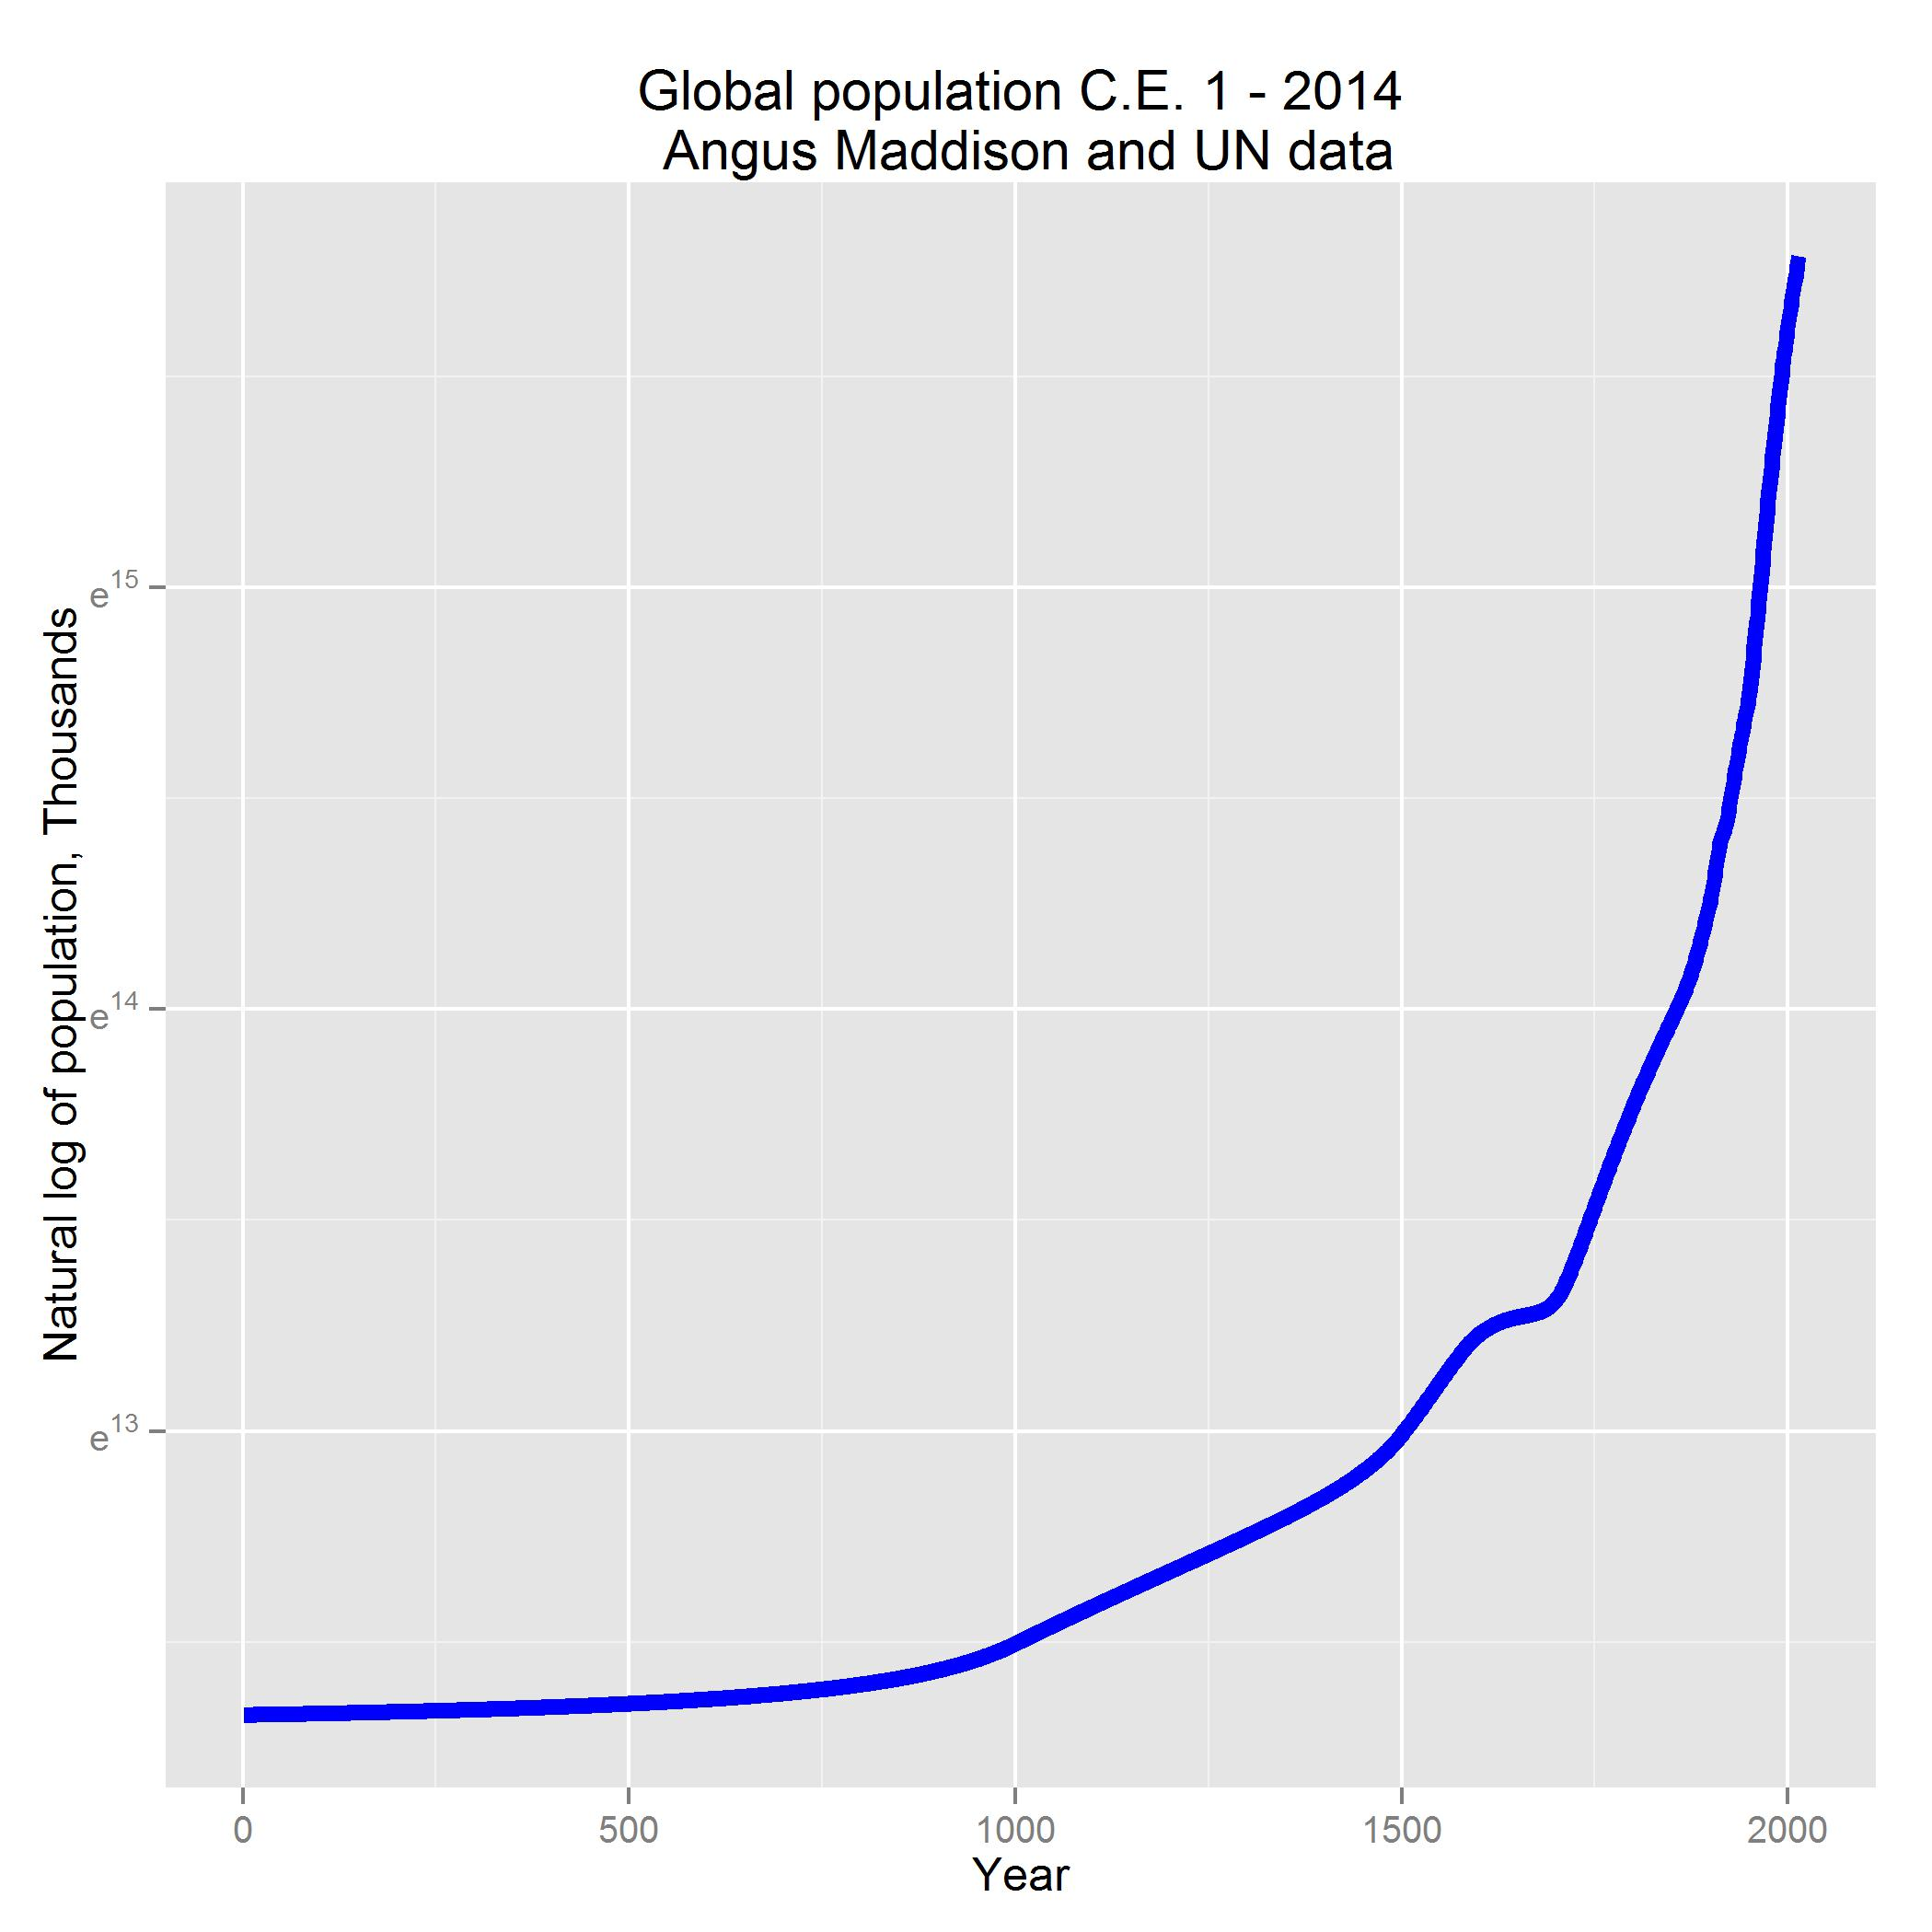
\includegraphics[width=0.60\textwidth]{C:/Users/Steve/Documents/GitHub/publish/diss3/images/logPop1-2014.jpg}}
		\mbox{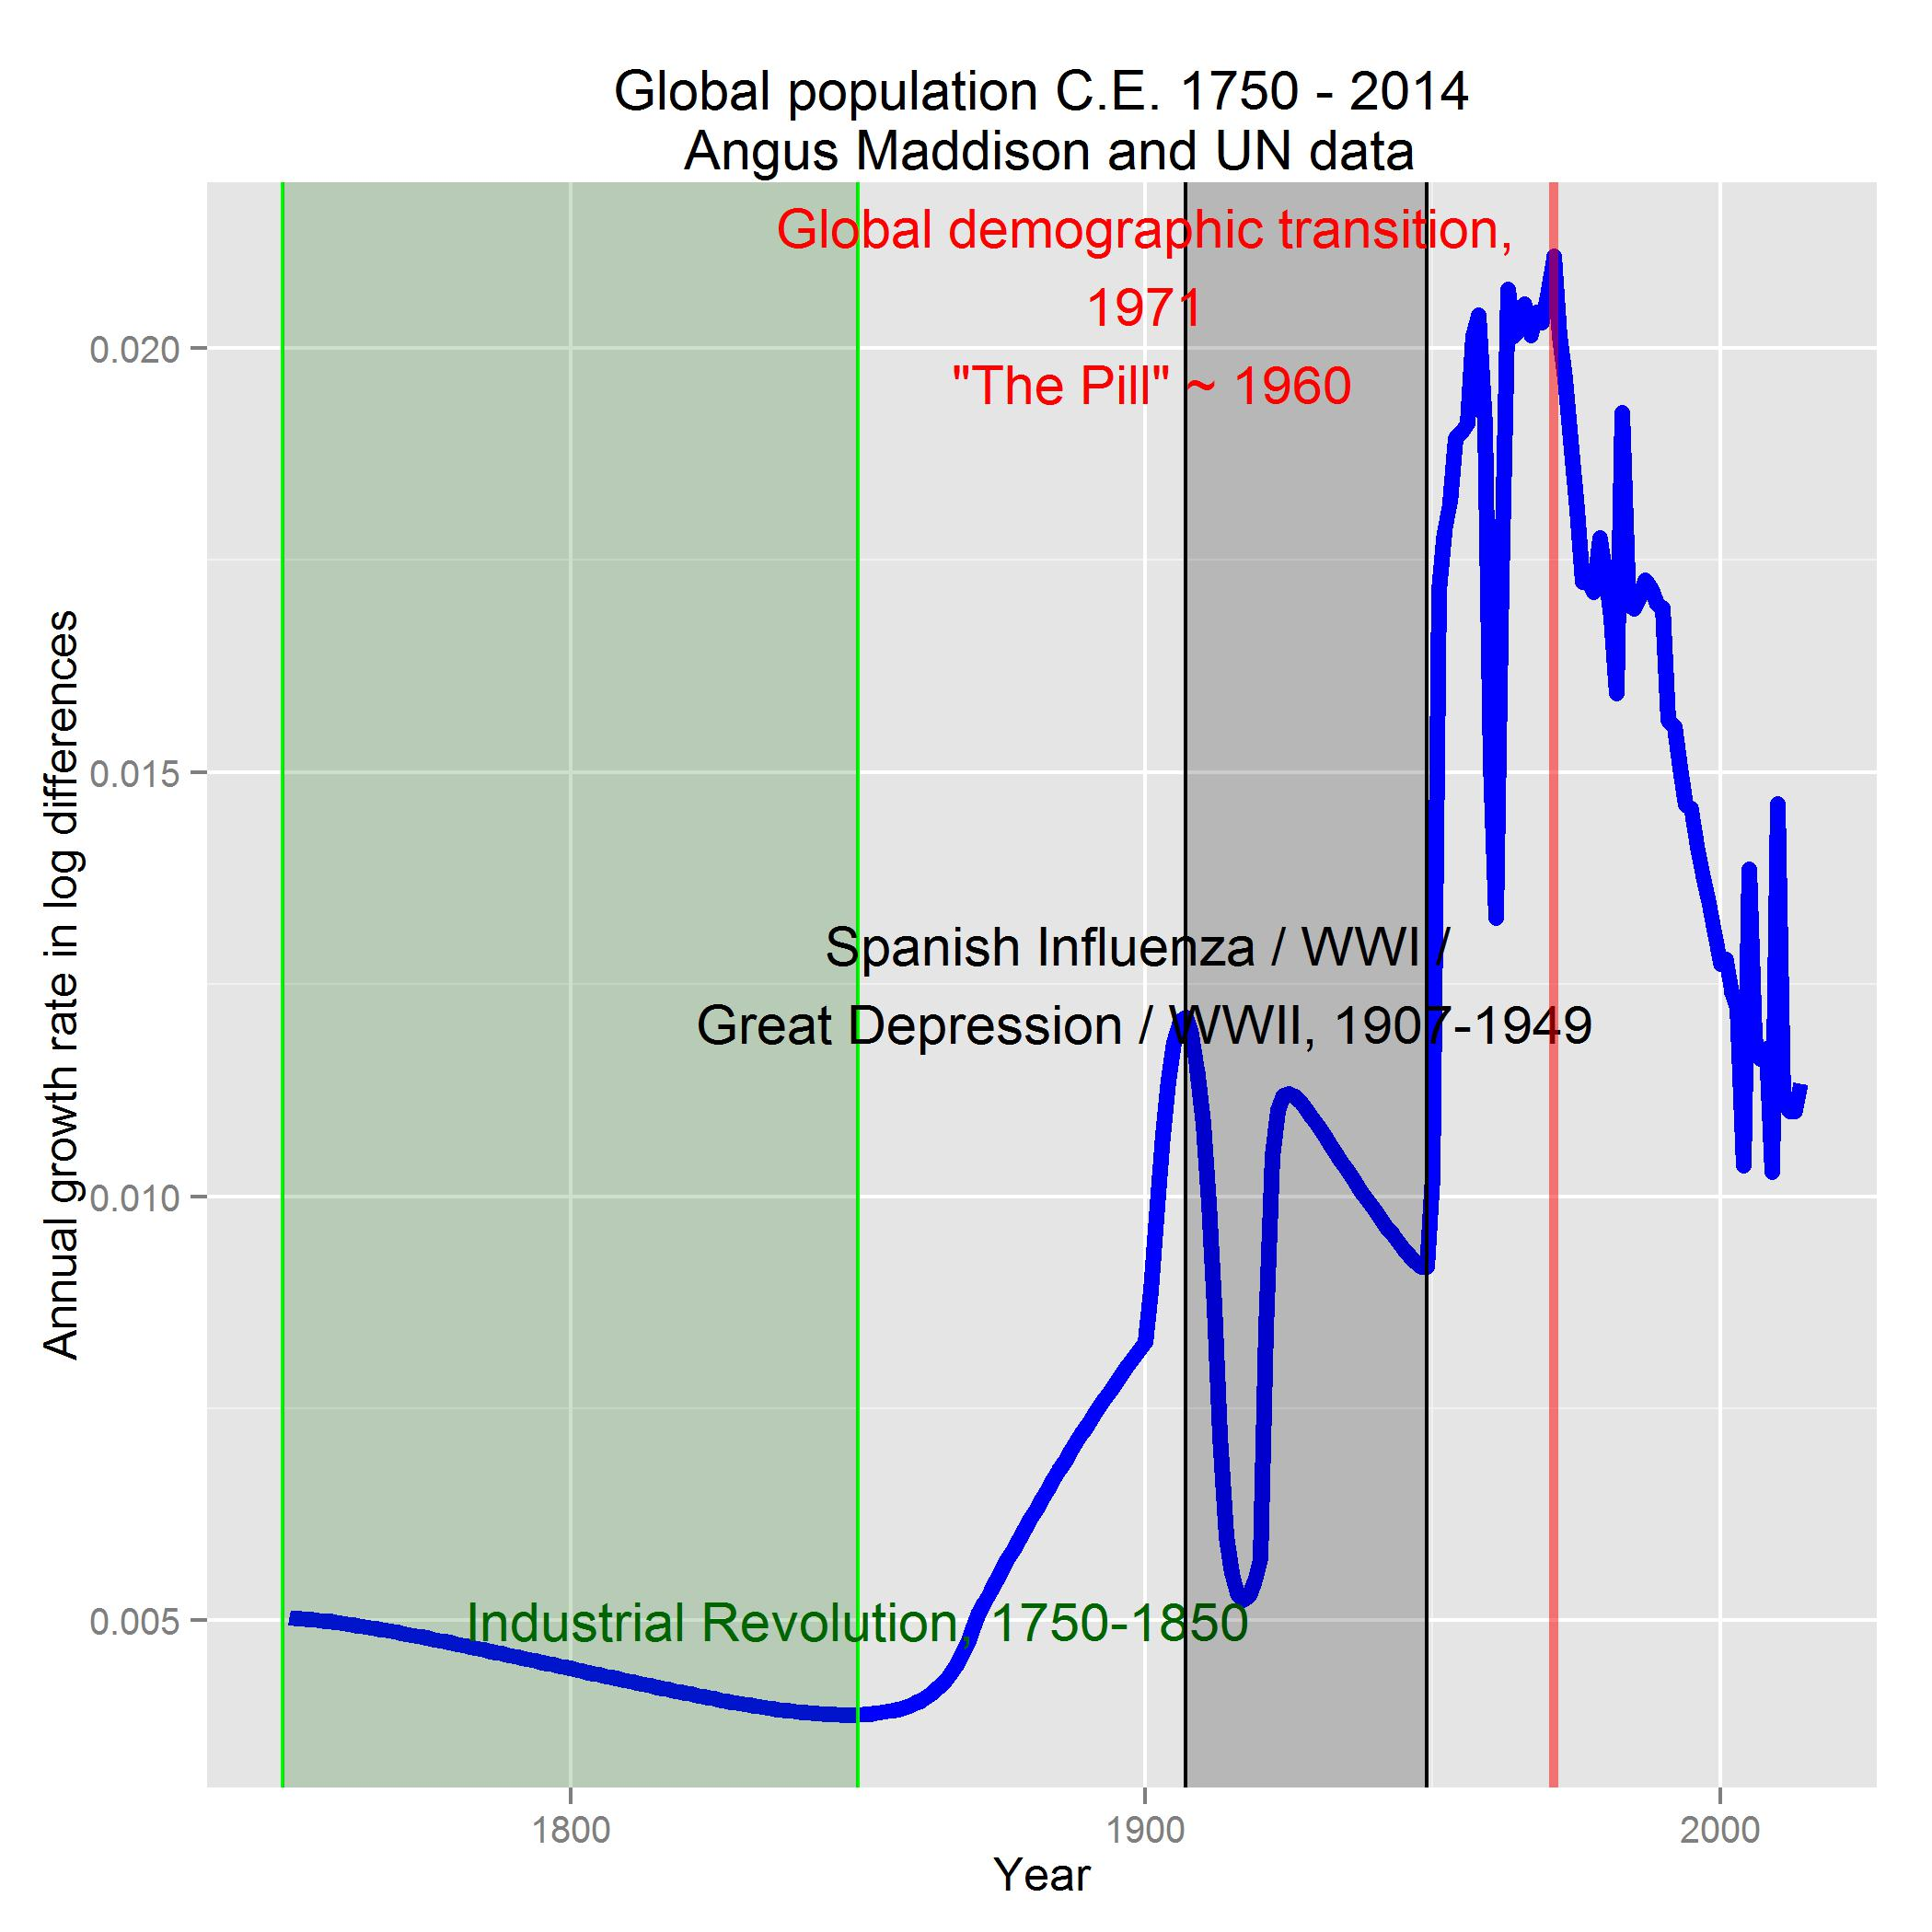
\includegraphics[width=0.60\textwidth]{C:/Users/Steve/Documents/GitHub/publish/diss3/images/logDiffPop1750-2014.jpg}}
		}
		\caption{Angus Maddison and UN: log and log differences of global population}
		\label{fig:logpoplevel}
		\end{figure}
		
		The left panel of figure \ref{fig:logpoplevel} displays the log of population levels since year one. This is super-exponential growth, with barely visible wiggles. This population, and thus aggregate demand, growth dynamic drove the supply side into the EIR and created industrial capitalism. The right panel is in log differences of annual population levels since 1750 (a common starting date for the EIR), so shows annual growth rates. Note that the growth rate peaked in 1971 at 2.2 percent, has declined to about 1 percent now, and appears poised to head, perhaps much, lower. If population growth was the underlying cause of industrial capitalism, then we must question the implications of its plummeting growth rate. I do so in a conjectural section in paper three.


After introductory comments, the essay's second section covers the important literature on this key intertwining of population dynamics-driven demand, supply-side economic responses, and the endogenous institutional growth arising from these powerful forces. The topics and authors covered in some depth are Karl Marx on Historical Materialism, Ruttan and Hayami on institutional endogeneity, a passing reference to Max Weber representing the vast institutionalist literature of all stripes, an in-depth review of Jan de Vries' excellent survey of (historically) recent thought on the industrial revolution and population dynamics, E.A. "Tony" Wrigley's significant contribution on both population dynamics and energy revolutions, and Nicholas Kaldor's contribution on essentialist causation.

Section three is a brief summary of the course of the EIR (generalized by my theoretical work); I have developed this story in other work included in this dissertation and I will not comment further here.

Section four develops the primary support for my claim that industrial capitalism was an outgrowth of the supply-side response to population dynamics during the relevant periods. Here I rely heavily on the work of three authors -- John Nef and Paul Mantoux on England, and John Hartwell on Sung China. None are commonly cited, an unfortunate oversight. Nef recounts the rise of the English coal industry, and directly comments in multiple passages that this economically-driven event caused industrial capitalism. Mantoux has very similar comments on the transition to machine industry using English textiles as an important frame. Hartwell covers the wood-to-coal revolution in the Sung Chinese iron industry including recounting the several rich Chinese families that financed the significant investments.

Given my theoretical framework, I organize this section according to the wood-to-coal transition (Nef and Hartwell) and the muscle-to-steam transition (Mantoux). These authors provide my main support for the primary claim of the essay.

Section five discusses capital's role in the EIR. This becomes a straightforward application of basic demand and supply laws. The primary story is the rise of demand for capital because of the energy revolutions; supply seemed never to be a true constraint.

Section six summarizes. Section seven contains my conjectures on industrial capitalism's future given my data on current population dynamics and the analysis in this essay.

Summarizing the claims in paper three,
%\renewcommand{\labelitemi}{$-$}
\begin{itemize}
\item[] I claim an economically essentialist cause for the EIR and industrial capitalism; this contradicts most historians, economic and other, who rely on cultural and institutional causes; these are of course important, but not, in my reading of the evidence, causal.
\item[] Summarizing and connecting the work of under-cited authors, the rise of the institution of industrial capitalism was caused first by rising aggregate demand due to population dynamics, second by the the supply-side response to this (several energy revolutions), and third by the need to finance the largest investments in economic history to meet the demand.
\item[] If rising consumer demand caused the the rise of industrial capitalism, then it may be logical and important to argue that falling consumer demand due to the reversal of the population dynamics that caused the rise will reverse the rise of industrial capitalism, a major, albeit speculative, claim.
\end{itemize}




\section{Postscripts to the general discussion -- insights for future work -- interesting questions:}

\begin{itemize}
\item[PS1] In evolving to an understanding of the EIR, one of my earliest explorations was the relationship between historical English Gross Domestic Product (GDP) and energy consumption. Having the good fortune of finding a new data series on English energy consumption starting in 1300, I found a very high correlation coefficient between that and GDP; this correlation is $0.998$. Statistically, there is no difference between these two data series. This leads me to surmise that this is perhaps the most important fundamental relationship on the supply side. Reflecting on this, it is not that surprising since energy input, no matter the source, is required for all economic, indeed all, activity. And these thoughts contrast fairly dramatically with Robert Solows's famous model in which his capital and labor inputs explained about fifteen percent of the output. Economic output seems tightly tied to thermodynamics, perhaps the truly important connection between economics and physics.
\item[PS2] Related to PS1, energy, again from any source, is non-substitutable. That is, you can change energy sources, and here economic theory describing input substitution works well, but you can not substitute away from energy however measured -- Joules, watt-hours, Million Tonnes of Oil Equivalents (MTOE), horsepower, human power, and so forth. Energy is perhaps the only essential input.
\item[PS3] Related to PS2, the theory of value comes to the fore, at least for me. What I claimed above is that it is the energy input that is fundamental to the production process. The source does not matter; a Joule is a Joule whether from a coal lump or a person, purely from the energy input perspective. Given this, what becomes of our theories of value? In particular the labor theory of value, via Smith, Ricardo, and most famously Marx, poses some issues given my claim. And I think these are real, but in order to really understand the implications, we need to categorize the types of labor, then redo the theory of value. Brad deLong offers an interesting taxonomy of the way humans add value:

\begin{enumerate}

    \item Using their strong (often testosterone-boosted) thigh, back, and shoulder muscles to move things around.
    \item Using their nimble fingers to finely-manipulate things.
    \item Using their brains as cybernetic-feedback control loops to make sure that the muscles, fingers, and machines do what they are supposed to do.
    \item Using their voices, smiles, and frowns to keep us as a group (roughly) on the same page and (roughly) pulling in the same direction.
	\item Fully using our brains to think of better ways and more useful ways to do things.
\end{enumerate}
Clearly one, two, and, with increasing automation, three are becoming less efficient for humans to do, so will be substituted away. Four could be jeopardized depending on artificial intelligence development. Five seems secure at the moment as it involves creativity, but is perhaps also susceptible. So most humans do, and have done, work that can be increasingly easily substituted to various machines. What does that do to the traditional theory of value? I do not have a clear answer; I do know the distribution implications are probably very large.

\item[PS4] In the third paper I explore a simple theory of a very important institution -- Industrial Capitalism. I use the basic economic principles of demand and supply. Demand for output has been increasing for a very long time as a function of growing population and living standards, driving the derived demand for productive capital stock upward. There appeared to be no big constraint on supply from the histories. Thus the rise of industrial capitalism in my telling was demand driven, and became sufficiently large that it caused the institution we call Industrial Capitalism. Fundamental economic change caused institutional change.

Beyond this example, I have thought considerably about institutions, and suspect that many are similarly endogenous to economic change. Further, institutions are inherently conservative, reactionary, or even repressive as they represent the powerful vested interests in societies. Conservative institutions, paraphrasing William Buckley, try to halt the progress of history. Reactionary ones try to turn history back. 

\item[PS5] Since production is a derived demand from final demand, we must make a statement about from where the demand driving the EIR came. I find it useful to think about two kinds of demand in this context: primary demand which is subsistence demand, enough to survive. Now I believe we should measure this in a cultural context; I recall that Brad deLong brought forward an idea of ``bio-cultural subsistence'' in a paper. This is close to what I want to think about. Because then, using that measure, I can measure secondary demand, which one can think of as living standards above bio-cultural subsistence.
\end{itemize}

\newpage
This page intentionally blank


\end{document}
%\SetWatermarkLightness{0.93}
%\SetWatermarkScale{1}

	\maketitle
%	\nocite{*}
%	\bibliographystyle{E:/LaTeX-Portable/MikTex-Portable/bibtex/bst/base/IEEEanot}

%	\bibliographystyle{E:/LaTeX-Portable/MikTex-Portable/bibtex/bst/base/plain-annote}
%	\bibliographystyle{plain}

\newcommand{\listequationsname}{List of Equations}
%\newlistof{myequations}{equ}{\listequationsname}
\newlistof{myequations}{equ}{\listequationsname}
\newcommand{\myequations}[1]{%
\addcontentsline{equ}{myequations}{\protect\numberline{\theequation}#1}\par}


	\begin{abstract}
	
	England, during the period leading up to and spanning the first Industrial Revolution, collectively learned how to consume a virtually unconstrained quantity of fossil (carbon) energy. Led by the period's effective aggregate demand growth, this led directly to productivity growth which then led to modern economic growth for the first time in recorded history. 
		
	Studying the event empirically, I use recent long-period series estimates of levels of English energy consumption, Gross Domestic Product, and population to test the hypothesis that this was primarily an \textit{energy} revolution with important but mostly proximate institutional and cultural support.
	
	The outcome should provide insights into economic development for development economists, highlighting the importance of energy transitions for growth of economic systems. Additionally, the analytic framework I develop can be applied across time and geography, adding insights to ongoing development puzzles.% and to the realistic chances of curbing ecologically damaging mineral (fossil) energy consumption for ecological economists and others interested in that critical topic.
	\end{abstract}
\section{Introduction}	%last

Unravelling the history of the English Industrial Revolution remains in the center ring of economic history. Beyond its historical significance, it holds major lessons for development economists in modern eras.

In this paper, I propose a methodological appeal to data-informed economic principles to explain the miracle. And I conclude that it was primarily an energy revolution; the English learned how to consume virtually unconstrained amounts of fossil energy. This directly led to modern economic growth for the first time in history.

Many, but not all, historians look to primarily institutional or cultural explanations for the event often expressed as a form of English exceptionalism; I propose a taxonomy in table \ref{tbl:taxonomy}. But this is not a paper about institutions; it is about economics. I try to make a strong case that while (a very few) necessary institutions were proximate, they were not sufficient, and do so by telling a compelling economic story, with economics often driving (endogenous) institutional change. The important exogenous institutional/cultural changes likely relate to expanded aggregate effective demand.

\begin{center}
Table \ref{tbl:taxonomy} about here
\end{center}

One must include Max Weber (\citeyear{weber_protestant_2002}) among the canonical exceptionalists, although indirectly bearing on England. Rather than lengthening this paper with details of this taxonomy, those will be in a forthcoming project. So I will proceed with the economics, acknowledging the few potentially causal cultural/institutional events that are required on the demand and supply sides.

As an important example of emphasizing how economic pressures led institutional changes, John Nef (\citeyear{nef_rise_1932}) relates how the economic pressure of English deforestation on wood prices influenced the post-English Reformation transfer of mineral-rich properties from the Church to the Crown, and the Crown's support of enclosures to consolidate mineral rights. Both of these ``institutional'' changes \textit{resulted} from economic pressures, improved the profitability of leasing mineral rights for coal and other mineral extraction, and thus had the macroeconomic result of an increase in the aggregate supply curve. A complete description of institutional changes must await further research.

The contributions I hope to make are to build a framework for analyzing the event which: coherently explains the event; can be extended to test the hypothesized importance of any institutional or cultural events; can accommodate new data series; proposes a structure of different energy/GDP regimes; re-dates the start of the event, moving it considerably earlier than many historians propose (John Nef excepted); uses statistical methods to understand the dynamics of the event; and applies macroeconomic and microeconomic theoretical principles to describe and explain the incentives embedded in this great and \textit{sui generis} event.

%\section{Variations on the story}
\section{Research questions} %1
I seek to identify empirically, economically, and eventually institutionally, what facts constituted the English Industrial Revolution. What was it, why did it occur, why did it happen when it did, why did it happen in England and only England? This paper addresses a subset of this agenda, describing what happened empirically, and suggesting the economic pressures and events that caused this result.

\section{Hypotheses}
The English Industrial Revolution (henceforth EIR) was the first example of modern economic growth (\cite{kuznets_modern_1966}). There were both macroeconomic and microeconomic forces that were causal. The primary driver of the EIR was an energy consumption revolution. There is limited statistical space for a very few exogenous causal institutional or cultural event clusters.	%2

I claim that the English Industrial Revolution was actually two related energy revolutions: the first substituted fossil mineral energy (coal) for wood for heat generation for both industrial and domestic uses; the second and later one substituted fossil mineral energy for labour energy inputs. Both were economically driven; the second one led directly to modern economic growth, and was enabled by the first.

\section{Research approach}
As this is a largely data-driven project, I first describe the data sources and comment on their limitations.

\subsection{Data}
Table \ref{tbl:dataSources} enumerates the primary data sources in this paper.
Figure \ref{fig:overall levels} displays the three data series keyed to the sources.

\begin{center}
Table \ref{tbl:dataSources} about here
\end{center}

The energy consumption data from Roger Fouquet covers England and Wales for the entire study period (1300 -- 1873). A word about why I end analysis in 1873: that is the end date Robert Allen (\citeyear{allen_british_2009}) places on the EIR. I can make a case from the data that it was a few years later, perhaps 1876, but there is little difference.

The gross domestic product data is composed from data series from Graeme Snooks and Lawrence Officer. The normalizing index is 2005 Great Britain Pounds. For this study period, those were the closest to England/Wales gross domestic product data that I have found.

The population data is composed from data series from Graham Snooks and Mitchell. For this study period, these were the closest to England/Wales population data I have found. Figure \ref{fig:overall levels} summarizes the data series by author/time-span.

\begin{center}
Figure \ref{fig:overall levels} about here
\end{center}

All such historical series are clearly composed, modelled, estimated, and thus fraught; a common problem with macroeconomic data to the present day. That said, I reserve special admiration in general for the work of the English economics historians. And these series are generally bounded by their starting point, their ending point, and various benchmarks along the way. The historians use a variety of methods to validate their work. In general, they cannot be too far wrong with the worst case being shifts by several decades in the shape of the curve. And the later data is generally better.

I do not claim these series are definitive for all time, simply the best I know of at this point, and possibly good enough. Their shapes clearly affect the analysis to follow. As better series appear, I will incorporate them into this analytic framework.

\begin{comment}
compare gdp, energy, pop series. table for sources\\
pop -- maddison vs. my current splice\\
gdp -- maddiosn vs. ?\\
e -- foquet vs. warde
\end{comment}

\subsection{Methodology}		%3
This paper uses largely descriptive statistics of the three data series to describe the EIR. Much of the discussion of results depends on the graphs. I do provide analytic statistics including correlations, sample tests, structural break analyses, bi-variate Granger causality tests (\cite{granger_investigating_1969}), and a scatterplot of energy consumption and gross domestic product. 

I also discuss the results in the context of microeconomic and macroeconomic theory, in a way consistent with the observed data.

I do not estimate a formal empirical model, such as a regression, as that seems redundant after examining the scatterplot. The correlation between energy consumption and gross domestic products is strikingly, and visibly, strong.

%In an appendix, I provide substantial time series analyses as a foundation for formal modelling when this work is extended to examining how

In a future version, I will provide substantial time series analyses as a foundation for formal modelling when this work is extended to examining how important certain historical events are in explaining the outcome. I believe that will be the best use of formal modelling; the approach in this paper is sufficient to support my stated hypothesis.

Anticipating the, potentially many, issues my claims will raise, I enumerate my known ones in a list summarized in table \ref{tbl:issues}. My goal, and hope, is that comments will either add issues to or remove them from the list. Further, I encourage comments on approaches to resolving these important historical issues.

\section{Results}		%6

\subsection{Modern economic growth}
Simon Kuznets defined modern economic growth as high rates of growth of per-capita product and population (\cite{kuznets_modern_1966}). Figures \ref{fig:ggdp} and \ref{fig:gdpLog} indicate that England experienced high rates of growth of per-capita product in (possibly) two eras, from 1500 to 1600 that was not sustained, and after 1750 that was mostly sustained. Clearly after about 1820 England had a high and sustained rate of growth in per-capita product here measured as gross domestic product. The annual rate after 1800 was 2.4 percent per-year total growth and 1.1 percent per-capita growth as seen in table \ref{tbl:growthByCentury}. Figure \ref{fig:popLog} shows the log of population growth which, supporting the Kuznets definition, mirrors GDP growth with a lag.

\begin{center}
Figures \ref{fig:ggdp} and \ref{fig:gdpLog} about here\\
Figure \ref{fig:popLog} about here\\
Table \ref{tbl:growthByCentury} about here
\end{center}



\subsection{An energy revolution}
This paper's central assertion is that the EIR was, primarily, an energy revolution. More generally, this was a consumer goods consumption revolution enabled by an energy supply revolution. To support that hypothesis, first I present the data:

Figure \ref{fig:energyLog} displays the log of energy consumption over the study period; the vertical lines are formally determined structural breaks.\footnote{The structural breaks use an F-test methodology on the time series as implemented in the $R$ package struccchange, \cite{zeileis_strucchange:_2002}} The log presentation enhances rate-of-change and potential structural differences in the series. I note four significantly different periods or regimes. The first is from 1300 to 1500, a period dominated by the Black Death epidemic; energy consumption clearly drops, then recovers. The second is from 1500 to roughly 1600 as determined by the structural break. The third is the period from 1600 to roughly 1750; note that the rate-of-change of energy growth in this period is approximately the same as in the prior period; this rate of change similarity is confirmed by the presentation in table \ref{tbl:growthByCentury}. The final period is from 1750 through 1873; clearly the energy consumption rate-of-change accelerates as confirmed by the structural breaks in figure \ref{fig:energyLog} and table \ref{tbl:growthByCentury}.

Based on the structural changes, and based on the hypothesis that the EIR was an energy revolution, I propose that the revolution happened as two main eras: one starting in the mid-to-late sixteenth century,\footnote{This validates John U. Nef's hypothesis of an early start to the British Industrial Revolution \cite{nef_rise_1932}}, and one starting after 1750. The first, under this hypothesis, would have set the stage for the second. The second could not have been possible without the first.

\begin{center}
Figure \ref{fig:energyLog} about here
\end{center}

If we were to overlay the energy levels or logs charts with the GDP levels or logs charts the similarities would be striking; I think a more productive view is figure \ref{fig:energyVsGdp}. This figure shows levels of energy consumption through the study period, and has a standardized series of GDP for the same period. By standardized I mean matched in levels at the first period; the series' evolutions thus show differences in growth rates through continuous time. Again we see four distinct regimes. The most notable features are the period of 1500 to 1600 when growth in GDP clearly leads energy growth, and after 1750 (especially after 1800), when energy growth leads GDP growth.

\begin{center}
Figure \ref{fig:energyVsGdp} about here
\end{center}

The dynamics of GDP growth and energy consumption growth can be seen more clearly by taking the differences of the last graph.

\begin{center}
Figure \ref{fig:energyVsGdpDiff} about here
\end{center}

The Black Death and its aftermath affected the relatively flat net economic performance from 1300 to 1500, but set the stage for a growth boom in the period 1500 to 1600. In the period 1600 to 1750 growth in both relatively flattened, and then boomed again during the period 1750 to 1873.

\subsection{Correlations}

Next, I present some simple analytic statistics to support the hypothesis that the EIR was at its root an energy revolution responding to a positive demand shock.

Starting simply, a Pearson's correlation coefficient and a paired t-test of energy consumption and GDP yields the results in table \ref{tbl:fitTest}: 

\begin{center}
Table \ref{tbl:fitTest} about here
\end{center}

%These simple results suggest that the two series are statistically very similar; a more formal co-integration test could be expected to be positive, and is presented as Appendix B in section \ref{app:Appendix B}. However, for the purposes of this paper, a scatterplot of the series 
These simple results suggest that the two series are statistically very similar; a more formal co-integration test could be expected to be positive, and will be  presented in a future version. However, for the purposes of this paper, a scatterplot of the series 
is shown in figure \ref{fig:scatterplot}. The solid green line is a linear fit; the solid red line is a \textit{lowess} (non-parametric, non-linear) fit.

\begin{center}
Figure \ref{fig:scatterplot} about here
\end{center}

Clearly, there is a very high correlation between the two series. For current purposes, more formal modelling is not needed. Overall statistically, these two series are very close to being the same, that is they share a common data generating process. In a strong sense this is a validation of the thermodynamic view of economic production and growth at least in the long run.

From an economics point of view, this graph suggests a Leontief, fixed-factors production function, which could also be consistent with a Sraffian production interpretation.

However, this overall view does hide important dynamics that the data contain. I examine these more subtle results next, and thereby set the stage for telling a history of the EIR.


\subsection{Causality tests}
I continue by using basic statistical causality tests, specifically the Granger bi-variate test to examine changing dynamics (\cite{granger_investigating_1969}). Table \ref{tbl:grangerEnergyGdp} reports this result for the four main eras already identified.

\begin{center}
Table \ref{tbl:grangerEnergyGdp} about here
\end{center}

During the first energy/GDP era Granger causality between energy and GDP runs both ways at significant levels; while not ignoring these results, I do not want to over-interpret what was happening given the huge shocks of the Black Death. However, it is significant for later eras that the Black Death caused wages to rise, and the European Marriage Pattern (EMP)(\cite{hajnal_european_1965}) increased family incomes entering the early modern period.

During the second energy/GDP era of 1500 to 1600 causality from GDP growth to energy consumption is weakly significant; energy Granger-causing GDP growth is not at all significant. However there is narrative evidence that this was an important proto-industrial period in which home manufacture for markets became important; this is the ``Industrious Revolution'' of Jan de Vries (\citeyear{de_vries_industrial_1994}). Further, there is evidence that the English state supported an early version of Import Substitution Industrialization to replace imports, and to export (\cite{thirsk_economic_1978}). These events support the idea that demand must have been growing, both in domestic consumption markets and for military goods from the government, and eventually for exports.

These events occurred in a backdrop of global population growth during a century of benign agricultural climate; croplands expanded, food was plentiful, real wages likely grew, nuptiality and fertility increased, and England participated in this bounty.

In the third energy/GDP era of 1600 to 1750, neither direction of causality is significant. This will turn out to have important implications as I build the history for the EIR.

In the fourth energy/GDP era of 1750 to 1873, we again see both directions of causality significant, with GDP Granger-causing energy consumption being the stronger.

Notably, over the entire study period GDP Granger-causes energy consumption more significantly than energy Granger-causes GDP, but causality is significant in both directions.

\subsection{Structural breaks}

Figure \ref{fig:structural} juxtaposes frames with logs of energy consumption, gross domestic product, and population, each with formal structural break lines noted. The point here is to note the correspondence of the structural breaks, again suggesting the same underlying data generating process, but with causality-implying lags.

\section{Discussion of results}

I can now present a story of the EIR as supported by the data presented above. 

\subsection{Narrative discussion}

Energy/GDP era one, due to the Black Death, saw both negative demand and supply shocks, but set the stage for the following EIR eras through long-term effects on wages, incomes, and effective aggregate demand. More broadly, the five centuries prior to era one comprise the Medieval Warming Epoch (or Period) supporting higher agricultural output and population levels, both supporting effective aggregate demand through expanded incomes. See figure \ref{fig:temps}.

\begin{center}
Figure \ref{fig:temps} about here
\end{center}


In energy/GDP era two, wages rose due to the negative labor supply shock of era one. Demand had positive shocks, as a result both of wages and  of incomes rising due to later marriages and women working -- the EMP outcomes -- and favorable agricultural conditions.  Expanded household production (\cite{de_vries_industrial_1994}) and explicit import substitution policies starting with Henry VIII, and continuing through Edward VI and Elizabeth I, supported increased aggregate demand. (\cite{thirsk_economic_1978}) See table \ref{tbl:monarchs} for reigns. Supply expanded as can be seen by the stronger growth of energy consumption. Refer to table \ref{tbl:growthByCentury} or figure \ref{fig:energyLog}. This era provided the positive demand shocks and supply constraints that caused the EIR. It started here.

John Nef amplifies this view. He tells the story of era two as the ``age of timber.'' The time frames are a bit different, he says ``\ldots no less appropriate to call the sixteenth and seventeenth centuries an age of timber'' (\citeyear{nef_rise_1932}, p.191). Nef tells a very rich story of rising use of timber for industrial and home heating use, and for construction, and the beginnings of a timber crisis. My dates for era two are 1500--1600, which Nef's dates overlap by going into my era three.

In energy/GDP era three, rates of growth for both GDP and energy consumptions stagnated. This still puzzles scholars including Braudel and Hobsbawm, but there are several potential stories that I will sketch out here. Returning to figure \ref{fig:temps}, notice that a decline in mean temperatures occurred in the early modern era. This era is called the Little Ice Age, and is believed to have been a global phenomenon. This would have opposite effects from the Medieval Warming Epoch, that is reduce agricultural output and population levels, and a negative aggregate demand shock due to reduced income levels. In a sense, this is also a negative energy supply shock, featuring reduced growing space and time due to less effective insolation.  

Scholarly discussion of both the Medieval Warming Epoch and the Little Ice Age seems concentrated among paleoclimatologists; yet they often refer to the effects on the economy, sometimes citing contemporaneous accounts. Jean Grove provides a survey in "The Little Ice Age " (\cite{grove_little_2003}). Hubert Lamb is often cited as an early researcher.\footnote{See, for example, \cite{lamb_aspects_1980}} Lamb describes failed grain harvests in Scotland, and the disappearance of the cod schools in the Atlantic. These examples are typical, though not the focus, in the climatology literature. They do provide a plausible economic explanation for the stagnation in GDP, and the lagged stagnation in population growth.

A related story that fits the data, and the history, is that this era was one of a negative energy supply shock due to deforestation, and growth in the whole economic system thus slowed. This era was the transition between primarily wood-supplied energy to primarily coal-supplied energy for industrial and home heat needs. As London grew because of internal growth, exports, and world trade domination, wood became scarcer and more expensive, driving demand for coal for heating from the north east. You can see this pattern during the 1600 to 1750 era three in the following figure \ref{fig:woodCoal}.

\begin{center}
Figure \ref{fig:woodCoal} about here
\end{center}

Notably, this is also the era Nef calls the ``first energy crisis'' (\cite{nef_early_1977}). During the period 1550 to 1700, according to Nef, increased heating and building demand for wood, and reduced woodlands due to agricultural demands, caused wood prices to rise dramatically.

We can hypothesize that this series of events provided the economic pressure to cause the first phase of the energy revolution -- the transition from wood to coal for heating needs.

A further potential explanation appeals to political events, mainly the large number of wars during the period. By and large the contemporary anecdotes were that war was economically stimulative (\cite{thirsk_economic_1978}). 

In the editing process for this paper, I reviewed further work of Jan de Vries, who reportedly denigrated any climatic explanation; in "The economy of Europe in an age of crisis, 1600-1750" de Vries indeed says the climate evidence is not consistent with population evidence; my work shows population lags GDP, which was plausibly affected by climate change, suggesting a more consistent data set. Separately, I note that my energy/GDP era three has the same year boundaries as de Vries (\citeyear{de_vries_economy_1976}). De Vries also has an extensive empirical look at Dutch temperatures and various measures of agricultural output. In the end he comes to few conclusions except that time-series data are essential, a conclusion I share (\cite{de_vries_measuring_1980}).

This demand for heating coal arising from the first energy crisis and the fortuitous geology of the English coal mines created the path necessary to support energy/GDP era four, in which the second phase of EIR accelerated into modern economic growth via the virtuous, mutually reinforcing, growth cycle between GDP and energy consumption. 

The geology story is that the coal mines were water-infused, and as they were dug deeper, more water had to be pumped out. This provided an economically feasible site for the seminal but very inefficient Newcomen steam engines to pump the water. The coal was essentially free to power the engines. Human or horse power were too expensive. And as the steam engines gained efficiency, they began to be applied to the products of industrial capitalism. That is the story of energy/GDP era four, the age of steam. I turn next to telling that story in more detail; again it is an economic story, supported by the data.


\subsection{Theory discussion}

We have already examined the GDP and energy consumption data for the fourth era. To finish the story, I will retreat to economic theory. First, I summarize the eras in aggregate supply/aggregate demand charts; second, I address the question of what caused the English inventor/entrepreneur to spend the time and money to make the inventions of the first and second phases of the EIR, particularly the steam engine. To do this, I appeal to standard microeconomic theory.

Figure \ref{fig:asad} displays the four eras in an aggregate demand/aggregate supply (AD/AS) framework. The dotted lines indicate prior locations of AD/AS; solid lines indicate the ending locations. Lines colored red indicate the constraint in each era. These are obviously abstract depictions of the history I have told above. I do this for two reasons; first to solidify and emphasize the history so that the debate can proceed; second to provide a framework for later projects incorporating the institutional and cultural events into the history. If we can agree on the AD/AS by era, then we can hypothesize about those events that might have caused the location or shape to change and then test those ideas in an econometric framework.


\begin{center}
Figure \ref{fig:asad} about here
\end{center}

A notable observation is that energy/GDP era four is the first in which supply was not the constraint; according to the Granger causality tests, supply and demand were jointly constraining in that era. Statistically, only GDP Granger-causing energy consumption is significant at normal levels, but the lack of relative barriers in consuming energy was surely the uniquely defining event of the era.

Second for the theoretical discussion of the EIR, it is important to consider at the microeconomic level what can explain the event. At this level I will discuss only the supply side having already suggested a story of the important demand-side factors. So the question becomes what were the incentives or motivations of the English inventors and entrepreneurs during energy/GDP eras two and three, so from 1500 through 1750.

For this analysis I rely on three sources; first the contemporaneous comments of a key participant in the EIR; second the excellent work of Robert Allen; and third an appeal to microeconomic theory.

Jean (or John) Theophilus Desaguliers had a large influence on the EIR. He was an eighteenth century English ``natural philosopher (physicist), member of the Royal Society, colleague of Sir Isaac Newton, and author of ``A Course of Experimental Philosophy.'' This was an influential 1734 two-volume engineering text that contained a chapter on ``Fire-Engines'' (steam engines). In this chapter, Jean Theophilus describes the economic and scalability motives of replacing men and horses with coal-fired steam engines to pump water out of Newcastle mines.  Profit was on his mind.  The age of the industrial capitalism, fueled by fossil energy, was dawning (\cite{desaguliers_course_1734}, vols. II, 467-468).

Figure \ref{fig:desagulier} shows a page of his manuscript.

\begin{center}
Figure \ref{fig:desagulier} about here
\end{center}

Beyond the quaintness of the 1734 English prose, this man demonstrated the soul of a profit-maximizing capitalist. In that context, let us examine some data that drove Desaguliers.

Figure \ref{fig:wage-energy} is from Robert Allen and shows the ratios of real wages to energy costs (the cheapest source) by benchmark city around 1700.

\begin{center}
Figure \ref{fig:wage-energy} about here\footnote{\cite{allen_british_2009}}
\end{center}

Clearly, Newcastle in 1700 had high wages and very low energy costs, by far the largest ratio in the sample. Those were the economic fundamentals that faced Desaguliers and motivated his profit comment. London had the second largest ratio, and thus the economic incentives existed there as well. Beijing had the lowest ratio, a topic I investigate in another research project.

While the economics of these ratios may be intuitive, why not appeal to microeconomic theory to help us understand what motivated Desaguliers, Newcomen, Watt and all the other founding fathers of the EIR. Equation \ref{eq:mrp} is a variation on production theory that will be familiar to those who remember their Econ 101. A major topic of mainstream production theory is how entrepreneurs maximize profits given the derived demand curves of the various input choices. 

This equation is a variation on that theme:\footnote{We can proceed either with a neo-classical factor substitution argument, or a more general classical view of normal prices of production. Either approach will react to the enormous productivity-enhancing energy supply shock that was the Industrial Revolution. A more challenging story to tell is one which identifies the sources of aggregate demand that supported expansion of English production. Here, I simply stipulate that aggregate demand existed.}


\begin{center}
Equation \ref{eq:mrp} about here
\end{center}

Instead of using different substitutable inputs such as labor and capital, I apply the theory to the different sources of energy, energy being essentially the only non-substitutable input as in you must have joules from whatever source to do any economic transformation. 

This equation is written as the profit-maximizing equilibrium that will substitute between different energy sources, say wood and coal for heating as wood becomes scarce; and, say, human-input joules replaced by coal-input joules as wages rise. Clearly, the equation needs additional terms to cover the amortization of whatever equipment is necessary to apply either kind of joule, but also clearly from just what is written we see that when wage-to-coal-energy cost ratios are sufficiently high, entrepreneur/inventors will be motivated to substitute coal joules for human joules. And that is what happened at the micro level to drive the EIR, first in Newcastle atop the mines, then in the English textile mills, then other English industries, later spreading to the world.


\section{Unresolved issues}
This essay is focused on exploring a data-driven economic explanation using energy inputs as primary in causing the Industrial Revolution. As space here is constrained, and given the claims the paper makes, there will be a (possibly very) large number of unresolved issues. I will initiate the list here as table \ref{tbl:issues}.

\begin{center}
Table \ref{tbl:issues} about here
\end{center}

In general E. A. Wrigley and John Nef have the most textured descriptions across the literature of what uniquely occurred in England which was a transition from, in Wrigley's terms, an advanced organic economy to an inorganic economy. So much of the reconciliation given my claims will be to Their work.

\section{Conclusion} %second last

The English Industrial Revolution, whatever else it was, was an \textit{energy consumption} revolution. This stands out as its primary feature, a feature that caused, for the first time in history, modern economic growth through large productivity gains. Mankind learned to consume energy in the economic process at a rate that was essentially unbounded, such that there was no longer an energy supply constraint on output.

This happened in England because England had a set of critical conditions that were rare: high wages, high family incomes, sufficient knowledge to construct ``Fire-Engines'', and very low relative energy costs with essentially unlimited supply. Of these critical factors, only England uniquely had very low relative energy costs; this last factor then must be deemed the necessary condition for the EIR.

The EIR happened in distinct eras, each of which can be defined as a specific energy/GDP (aggregate supply -- aggregate demand) regime which frames further research on what exogenous institutions and other factors may have been important. We can use data and simple macroeconomic principles to usefully investigate the EIR. England collectively ``learned'' how to create a positive virtuous macroeconomic growth feedback cycle driven by fossil energy consumption.

Also, there were two distinct energy transitions which are intertwined in a path-dependent story: the first substituting coal for wood in domestic and industrial heating uses; and the second substituting coal energy for labour energy in industrial mechanical uses enabled initially by the steam engine.

Further, the individual behavior of the EIR inventors and entrepreneurs can be explained using simple microeconomic principles. 

Given all this, extant hypotheses of English cultural and/or institutional exceptionalism seem redundant to the outcome. England was a very lucky country, geographically advantaged, at the right place and time for this miracle to occur.

\begin{comment}
\section{journal strategy}
Possible journals:\\
Explorations in Economic History, Economic History Review (European), Journal of Economic History, Cliometrica.\\
Non-history:\\
development journals that accept history?\\
energy journals that accept history?\\
Science? Nature?\\
Reynolds suggests going for AER!\\
Journal of Applied Econometrics (Dave Giles)\\
Journal of International Trade and Economic Development (Dave Giles)\\
\end{comment}

\section{References}
		\bibliographystyle{agsm}	
	\bibliography{diss2}

\listoftables

\listoffigures

\listofmyequations

\newpage

\section{Tables}

\begin{table}[p!]
\caption{Taxonomy of EIR explanations}
\label{tbl:taxonomy}
\begin{tabular}{rl}
Label&Examples\\
\hline
English exceptionalists&Landes (1969), McCloskey (2010), Mokyr (1992,2010)\\
Partial culturalists&Cipolla (1966), Pomeranz (2001), Allen (2009)\\
Primarily energetic&Cottrell (1955), Wrigley (1988,2010), Malanima (2010), Nef (1932)\\
Thermodynamicists&Georgescu-Roegen (1975), Ayres (2003), Garrett (2009)\\
\end{tabular}
\end{table}


\begin{table}[p!]
\caption{Data Sources}
\label{tbl:dataSources}
\begin{tabular}{lrll}
Data series&Year range&Geography&Source\\
\hline
Energy consumption&1300 -- 1873&England/Wales&Roger Fouquet (2008)\\
\hline
Gross domestic product&1300 -- 1700&England&Graeme Snooks (1994)\\
&1741 -- 1873&England/Wales&Lawrence Officer (2009)\\
\hline
Population&1300 -- 1540&England&Graeme Snooks (1994)\\
&1541 -- 1800&England&B. R. Mitchell (1988)\\
&1801 -- 1873&England/Wales&B. R. Mitchell (1988)\\
\end{tabular}
\end{table}

\begin{comment}
\begin{table}[p!]
\caption{t-test of energy and gdp}
\label{tbl:t-testEnergyGdp}
\begin{tabular}{rl}
\end{tabular}
\end{table}
\end{comment}

\begin{table}[p!]
\caption{Wood and total price indices. \textit{Source:} Nef (1932, p.158,221)}
\label{tbl:woodPrice}
\center
\begin{tabular}{lrr}
Period&General price index&Wood price index\\
\hline
1451-1500&100&100\\
1531-1540&105&94\\
1551-1560&132&163\\
1583-1592&198&277\\
1603-1612&251&366\\
1613-1622&257&457\\
1623-1632&282&677\\
1633-1642&291&780\\
1643-1652&331&490\\
1653-1662&308&662\\
1663-1672&324&577\\
1673-1682&348&679\\
1683-1692&319&683\\
1693-1702&339&683\\
\end{tabular}
\end{table}


\begin{table}[p!]
\caption{growth rates by century}
\label{tbl:growthByCentury}
\begin{tabular}{lrrrrrrrr}
Year	&	1300	&	1400	&	1500	&	1600	&	1700	&	1801	&	1873&Total	\\
\hline
GDP Million\\ 2005 GBP	&	3114.7541	&	815.1288	&	994.4571	&	6031.953	&	8361.5911	&	18110	&	102811&	\\
Century-over-century\\rate of growth&&-0.738&0.220&5.066&0.386&1.166&4.677&32.008\\
Compounded annual \\rate of growth&&-0.013&0.002&0.018&0.003&0.008&0.024&0.006\\
\hline
Energy consumption&1.7	&	1	&	1.3	&	2.2	&	3.6	&	11.6	&	66.1&	\\
Century-over-century\\rate of growth&&-0.412&0.300&0.692&0.636&2.222&4.698&37.882\\
Compounded annual \\rate of growth&&-0.005&0.0026&0.005&0.005&0.012&0.024&0.006\\
\hline
Per-capita GDP\\2005 GBP&542&  329&  421& 1,484& 1,663& 1,999& 4,392\\
Century-over-century\\rate of growth&&-0.393& 0.282&2.521&0.121&0.202&1.198& 7.108\\
Compounded annual \\rate of growth&&-0.005&0.002&0.013&0.001&0.002& 0.011&0.004\\
\end{tabular}
\end{table}

\begin{table}[p!]
\caption{Energy and GDP fit tests}
\label{tbl:fitTest}
\begin{center}
\begin{tabular}{lrr}
\hline\hline
Test&Statistic&p-value\tabularnewline
\multicolumn{1}{c}{}\tabularnewline
\hline
Pearson's correlation&$0.998$&\tabularnewline
\hline
Paired t-test&$5.592$&4.991e-07\tabularnewline
\hline
Chi-square&2864&0.0004998\tabularnewline
\end{tabular}
\end{center}
\end{table}

\begin{table}[p!]
\caption{granger tests of energy/gdp}
\label{tbl:grangerEnergyGdp}
\begin{tabular}{lrrl}
Era&Energy $\sim$ GDP Pr($>$F)& GDP $\sim$ Energy Pr($>$F)&AD/AS regime\\
\hline
1300 -- 1500&0.0106&0.0003&EMP, Black Death, \\&&&wages/family income increasing\\
1500 -- 1600&0.1939&0.6126&Positive demand shock\\
1600 -- 1750&0.3529&0.5185&Energy supply constraint\\
1750 -- 1873&0.0024&0.1100&Positive supply shock,\\&&&``virtuous'' macro feedback cycle\\
\hline
1300 -- 1873& 0.0002& 0.0361&Total study period\\
\end{tabular}
\end{table}

\begin{table}[p!]
\caption{Unresolved issues}
\label{tbl:issues}
\center
\begin{tabular}{ll}
Issue&Comment\\
\hline
Reconcile to 1970 English energy study&Humphrey and Stanislaw\\
Reconcile to Broadberry et al. on agricultural revolution, growth&Broadberry et al. vs. PBH\\
Reconcile to English agricultural revolution&Wrigley is the starting place\\
Effects of ``Columbian Exchange'' &Crosby\\
(e.g. potatoes) on English agriculture&\\
Reconcile to English urbanization&Again, Wrigley\\
Paradox of short nineteenth century heights&mentioned by deLong\\
Reconcile to narrow industry energy scope&McCloskey\\
Address general purpose technology story&Bresnehan\\
Reconcile to Nef data&John U. Nef\\
Reconcile to ``little ice age''&de Vries\\
Reconcile to Marc Braudel&Marc Braudel\\
\hline
\end{tabular}
\end{table}

\begin{table}[p!]
\caption{Early modern English monarchs}
\label{tbl:monarchs}
\center
\begin{tabular}{lll}
Monarch&Reign&House\\
\hline
Henry VIII&1509-1547&Tudor\\
Edward VI&1547-1553&Tudor\\
Mary I&1553-1558&Tudor\\
Elizabeth I&1558-1603&Tudor\\
James I&1603-1625&Stuart\\
Charles I&1625-1649&Stuart\\
Oliver Cromwell&1653-1658&Commonwealth\\
Richard Cromwell&1658-1659&Commonwealth\\
Charles II&1660-1685&Stuart\\
James II&1685-1688&Stuart\\
Mary II&1689-1694&Stuart\\
William III&1689-1702&Stuart\\
Anne&1702-1707&Stuart\\
\hline
\end{tabular}
\end{table}


\newpage

\section{Figures}

\begin{figure}[p!]
\center
\caption{Author/time-span series of energy consumption, GDP, and population}
\label{fig:overall levels}
\includegraphics[width=0.9\textwidth]{overallLevels}
\end{figure}

		\begin{figure}[p!]
		\caption{English real gross domestic product, \\
		levels and per--capita }
		\label{fig:ggdp}		
		\centerline{
		\mbox{\includegraphics[width=0.55\textwidth]{ggdp}}
		\mbox{\includegraphics[width=0.55\textwidth]{ggdppop}}
		}
		\end{figure}

		\begin{figure}[p!]
		\caption{English real gross domestic product, \\
		log levels and log per--capita}
		\label{fig:gdpLog}		
		\centerline{
		\mbox{\includegraphics[width=0.55\textwidth]{gdpLog}}
		\mbox{\includegraphics[width=0.55\textwidth]{gdpPopLog}}
		}
		\end{figure}

\begin{figure}[p!]
\center
\caption{Log of population, with structural breaks}
\label{fig:popLog}
\includegraphics[width=0.9\textwidth]{popLog}
\end{figure}

\begin{figure}[p!]
\center
\caption{Log of energy consumption, with structural breaks}
\label{fig:energyLog}
\includegraphics[width=0.9\textwidth]{energyLog1.png}
\end{figure}

\begin{figure}[p!]
\center
\caption{Energy consumption vs. standarized GDP}
\label{fig:energyVsGdp}
\includegraphics[width=0.9\textwidth]{energyVsGdp}
\end{figure}

\begin{figure}[p!]
\center
\caption{Energy consumption vs. standardized GDP, differences}
\label{fig:energyVsGdpDiff}
\includegraphics[width=0.9\textwidth]{energyVsGdpDiff}
\end{figure}

\begin{figure}[p!]
\center
\caption{Scatterplot of energy consumption vs. GDP}
\label{fig:scatterplot}
\includegraphics[width=0.9\textwidth]{scatterplot.png}
\end{figure}

\begin{figure}[p!]
		\caption{Structural break comparison}
		\label{fig:structural}		
		\centerline{
		\mbox{\includegraphics[width=0.33\textwidth]{energyLog1}}
		\mbox{\includegraphics[width=0.33\textwidth]{gbpgdplog}}
		\mbox{\includegraphics[width=0.33\textwidth]{popLog}}
		}
\end{figure}

\begin{figure}[H]
\center
\caption{Late Holocene temperatures. \textit{source:} NASA and IPCC composite}
\label{fig:temps}
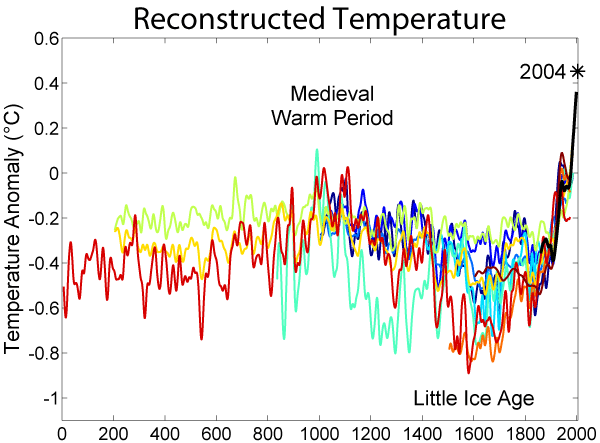
\includegraphics[width=0.9\textwidth]{2000_Year_Temperature_Comparison.png}
\end{figure}

\begin{figure}[h!]
\center
\caption{Coal and wood energy sources\\\textit{Source:} Pearson \& Fouquet}
\label{fig:woodCoal}
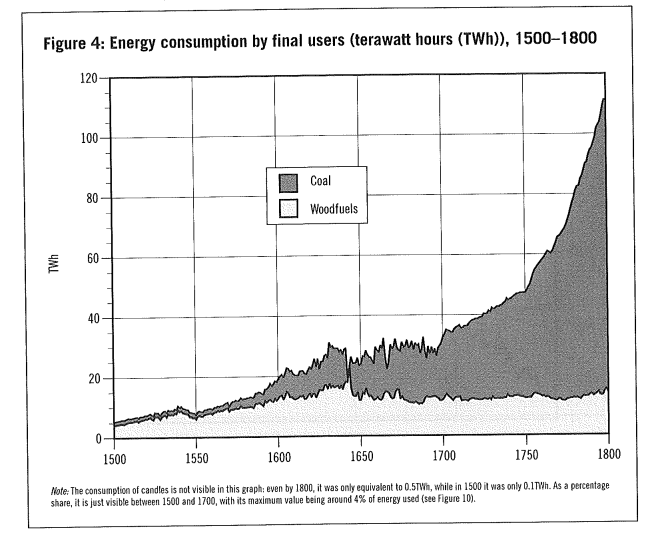
\includegraphics[width=0.9\textwidth]{woodCoal.png}
\end{figure}

\begin{figure}[h!]
		\caption{Aggregate Supply - Aggregate Demand \\ Four energy/GDP regimes}
		\label{fig:asad}		
		\centerline{
		\mbox{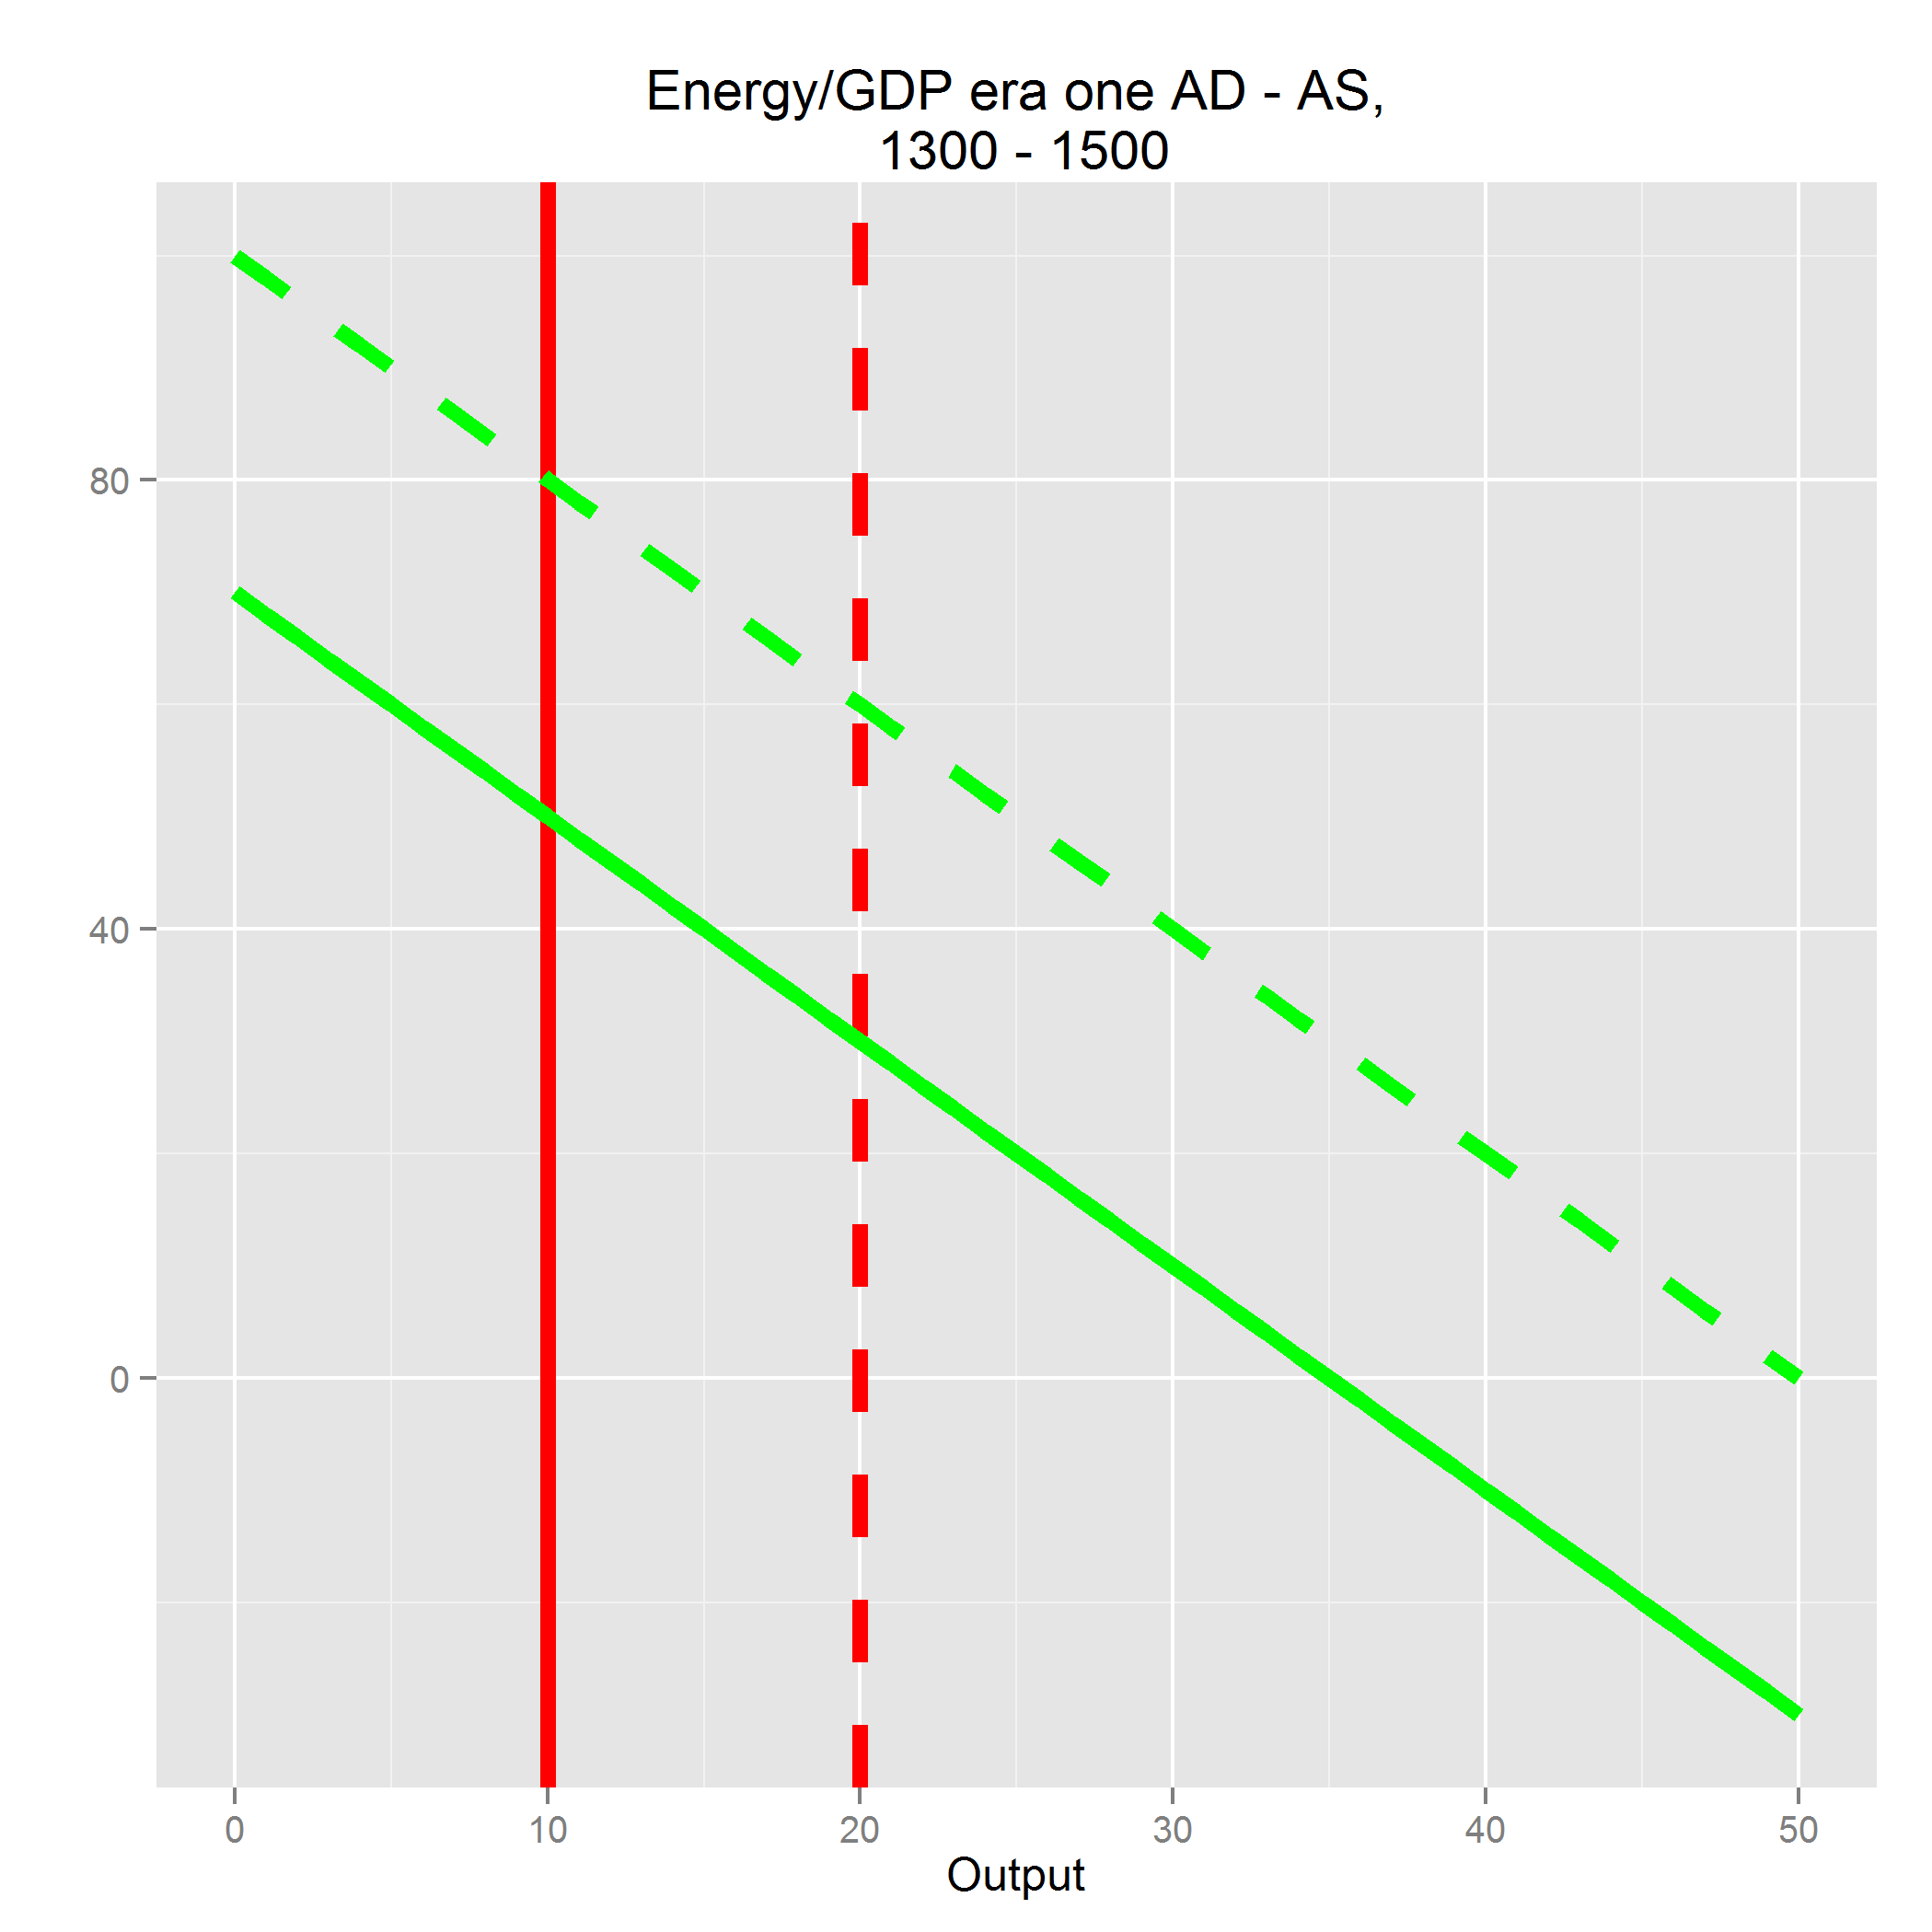
\includegraphics[width=0.25\textwidth]{era1}}
		\mbox{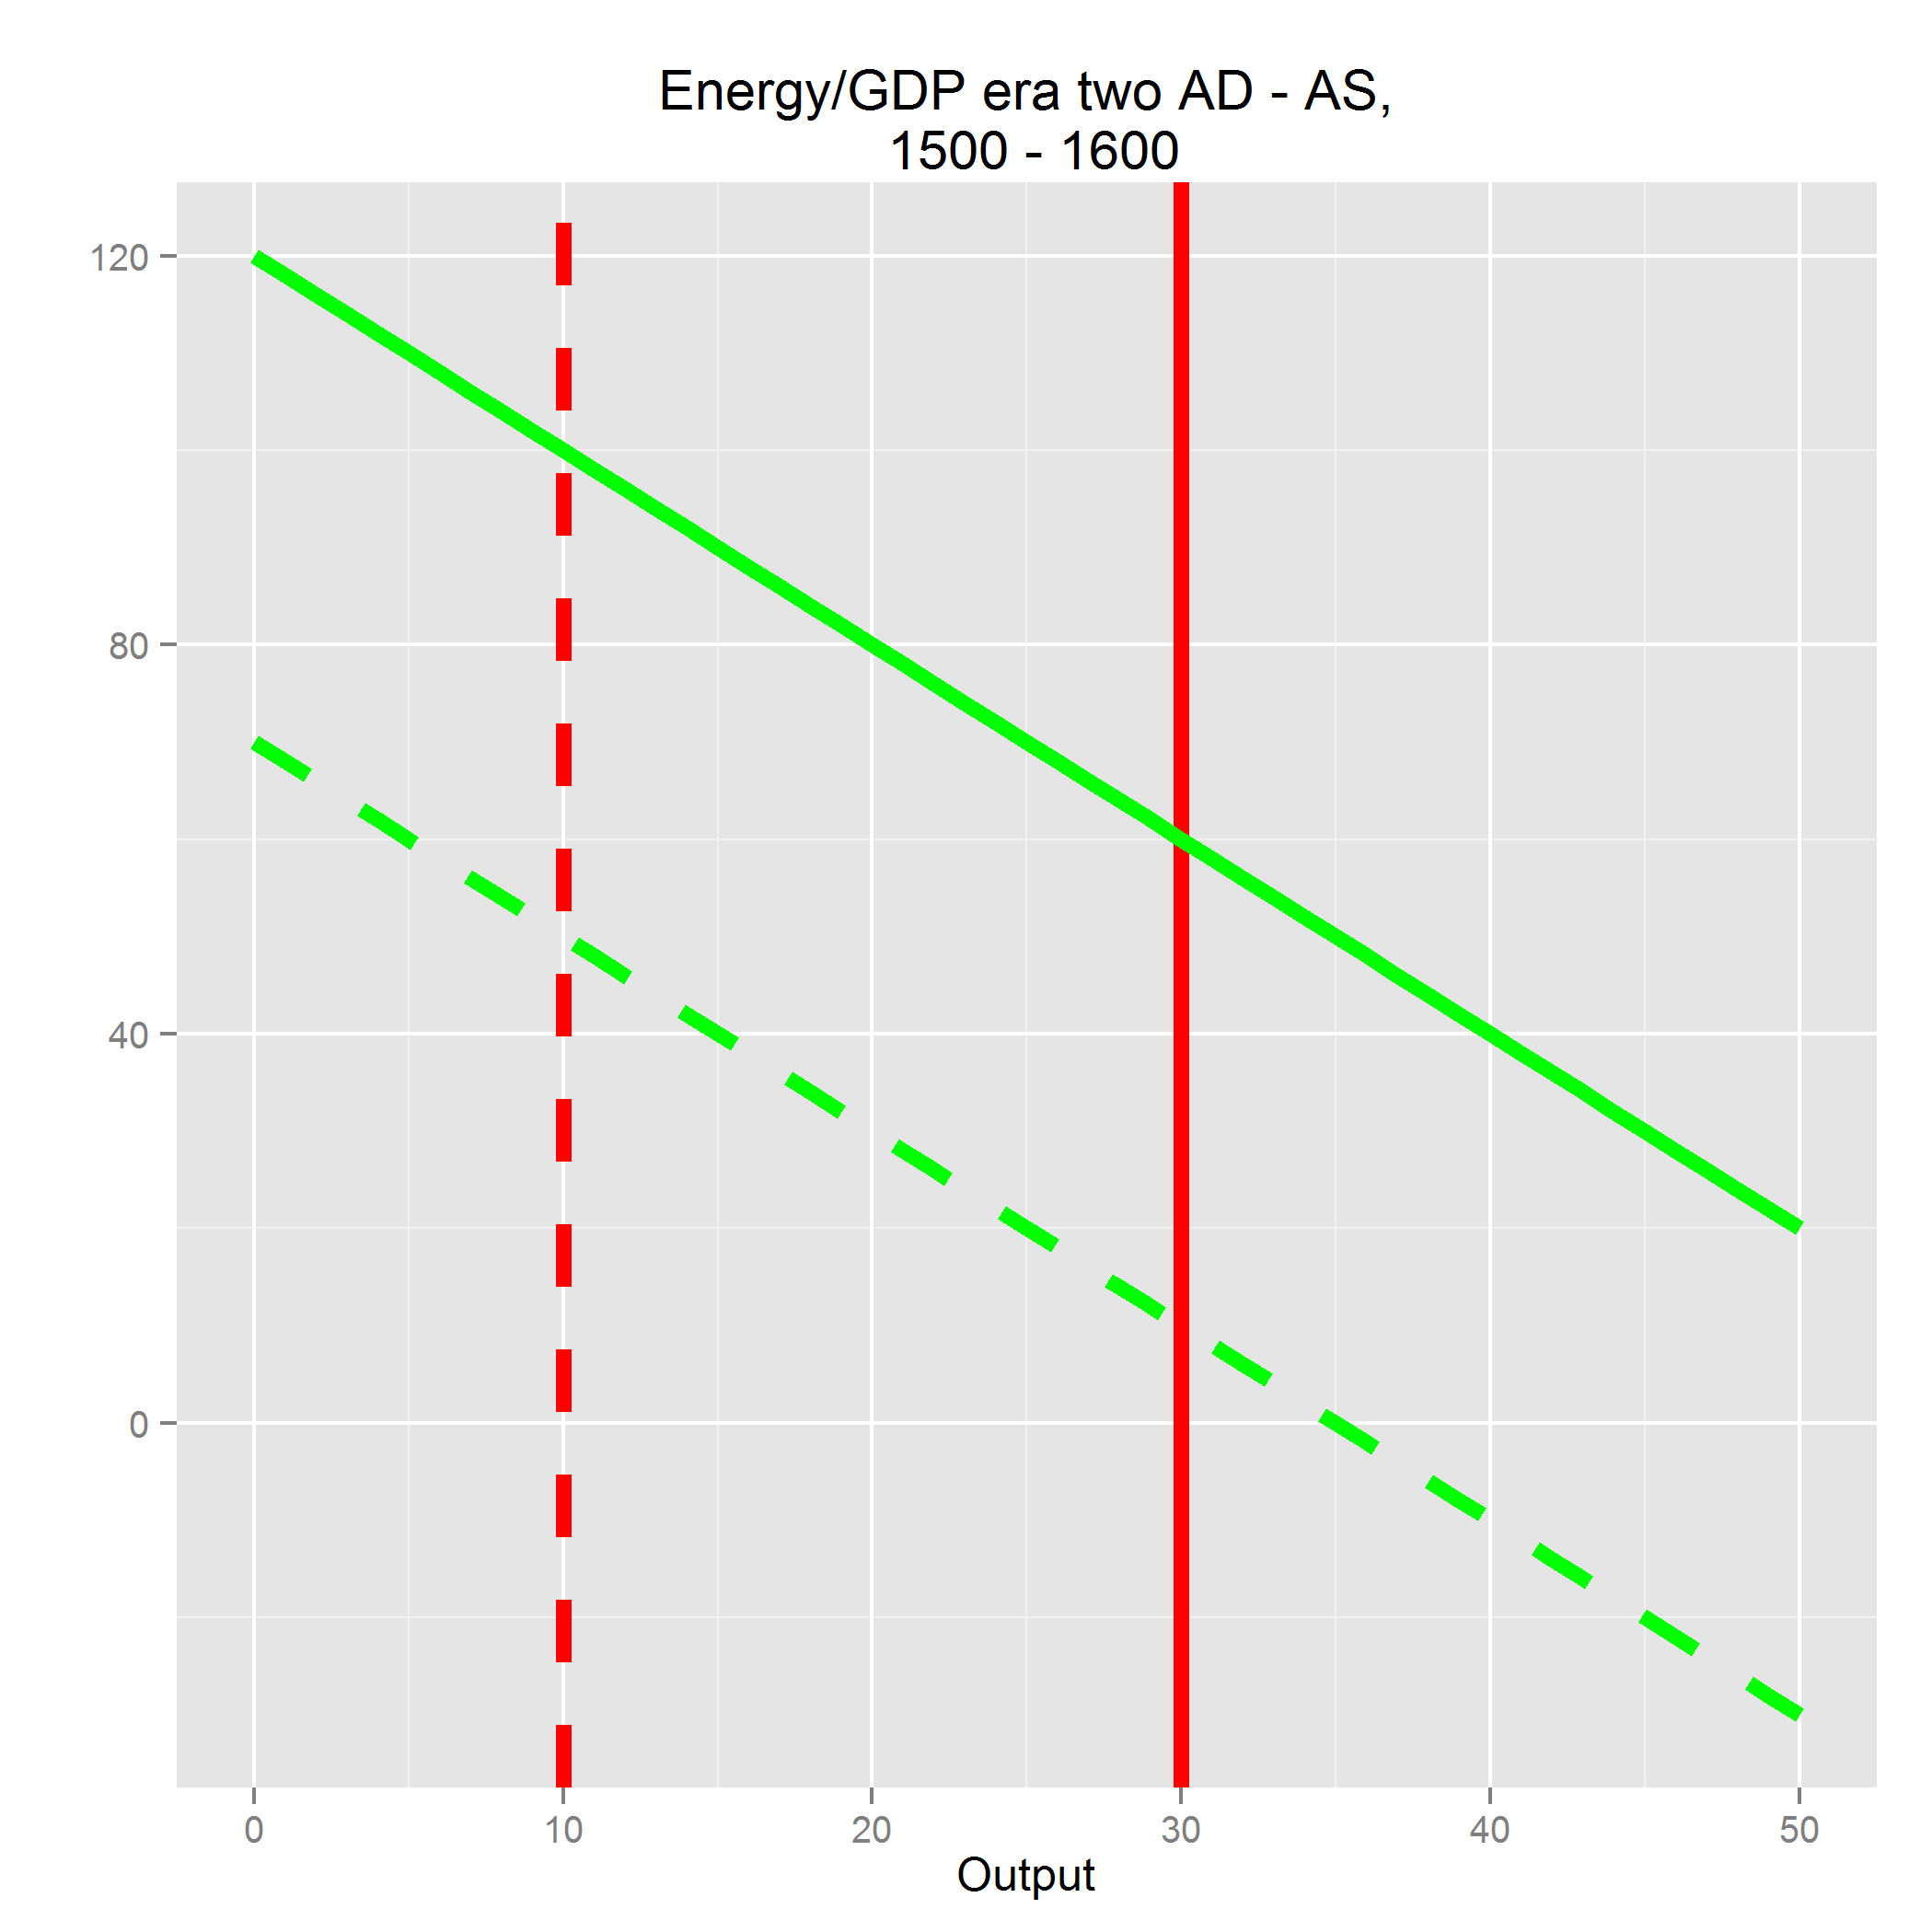
\includegraphics[width=0.25\textwidth]{era2}}
		\mbox{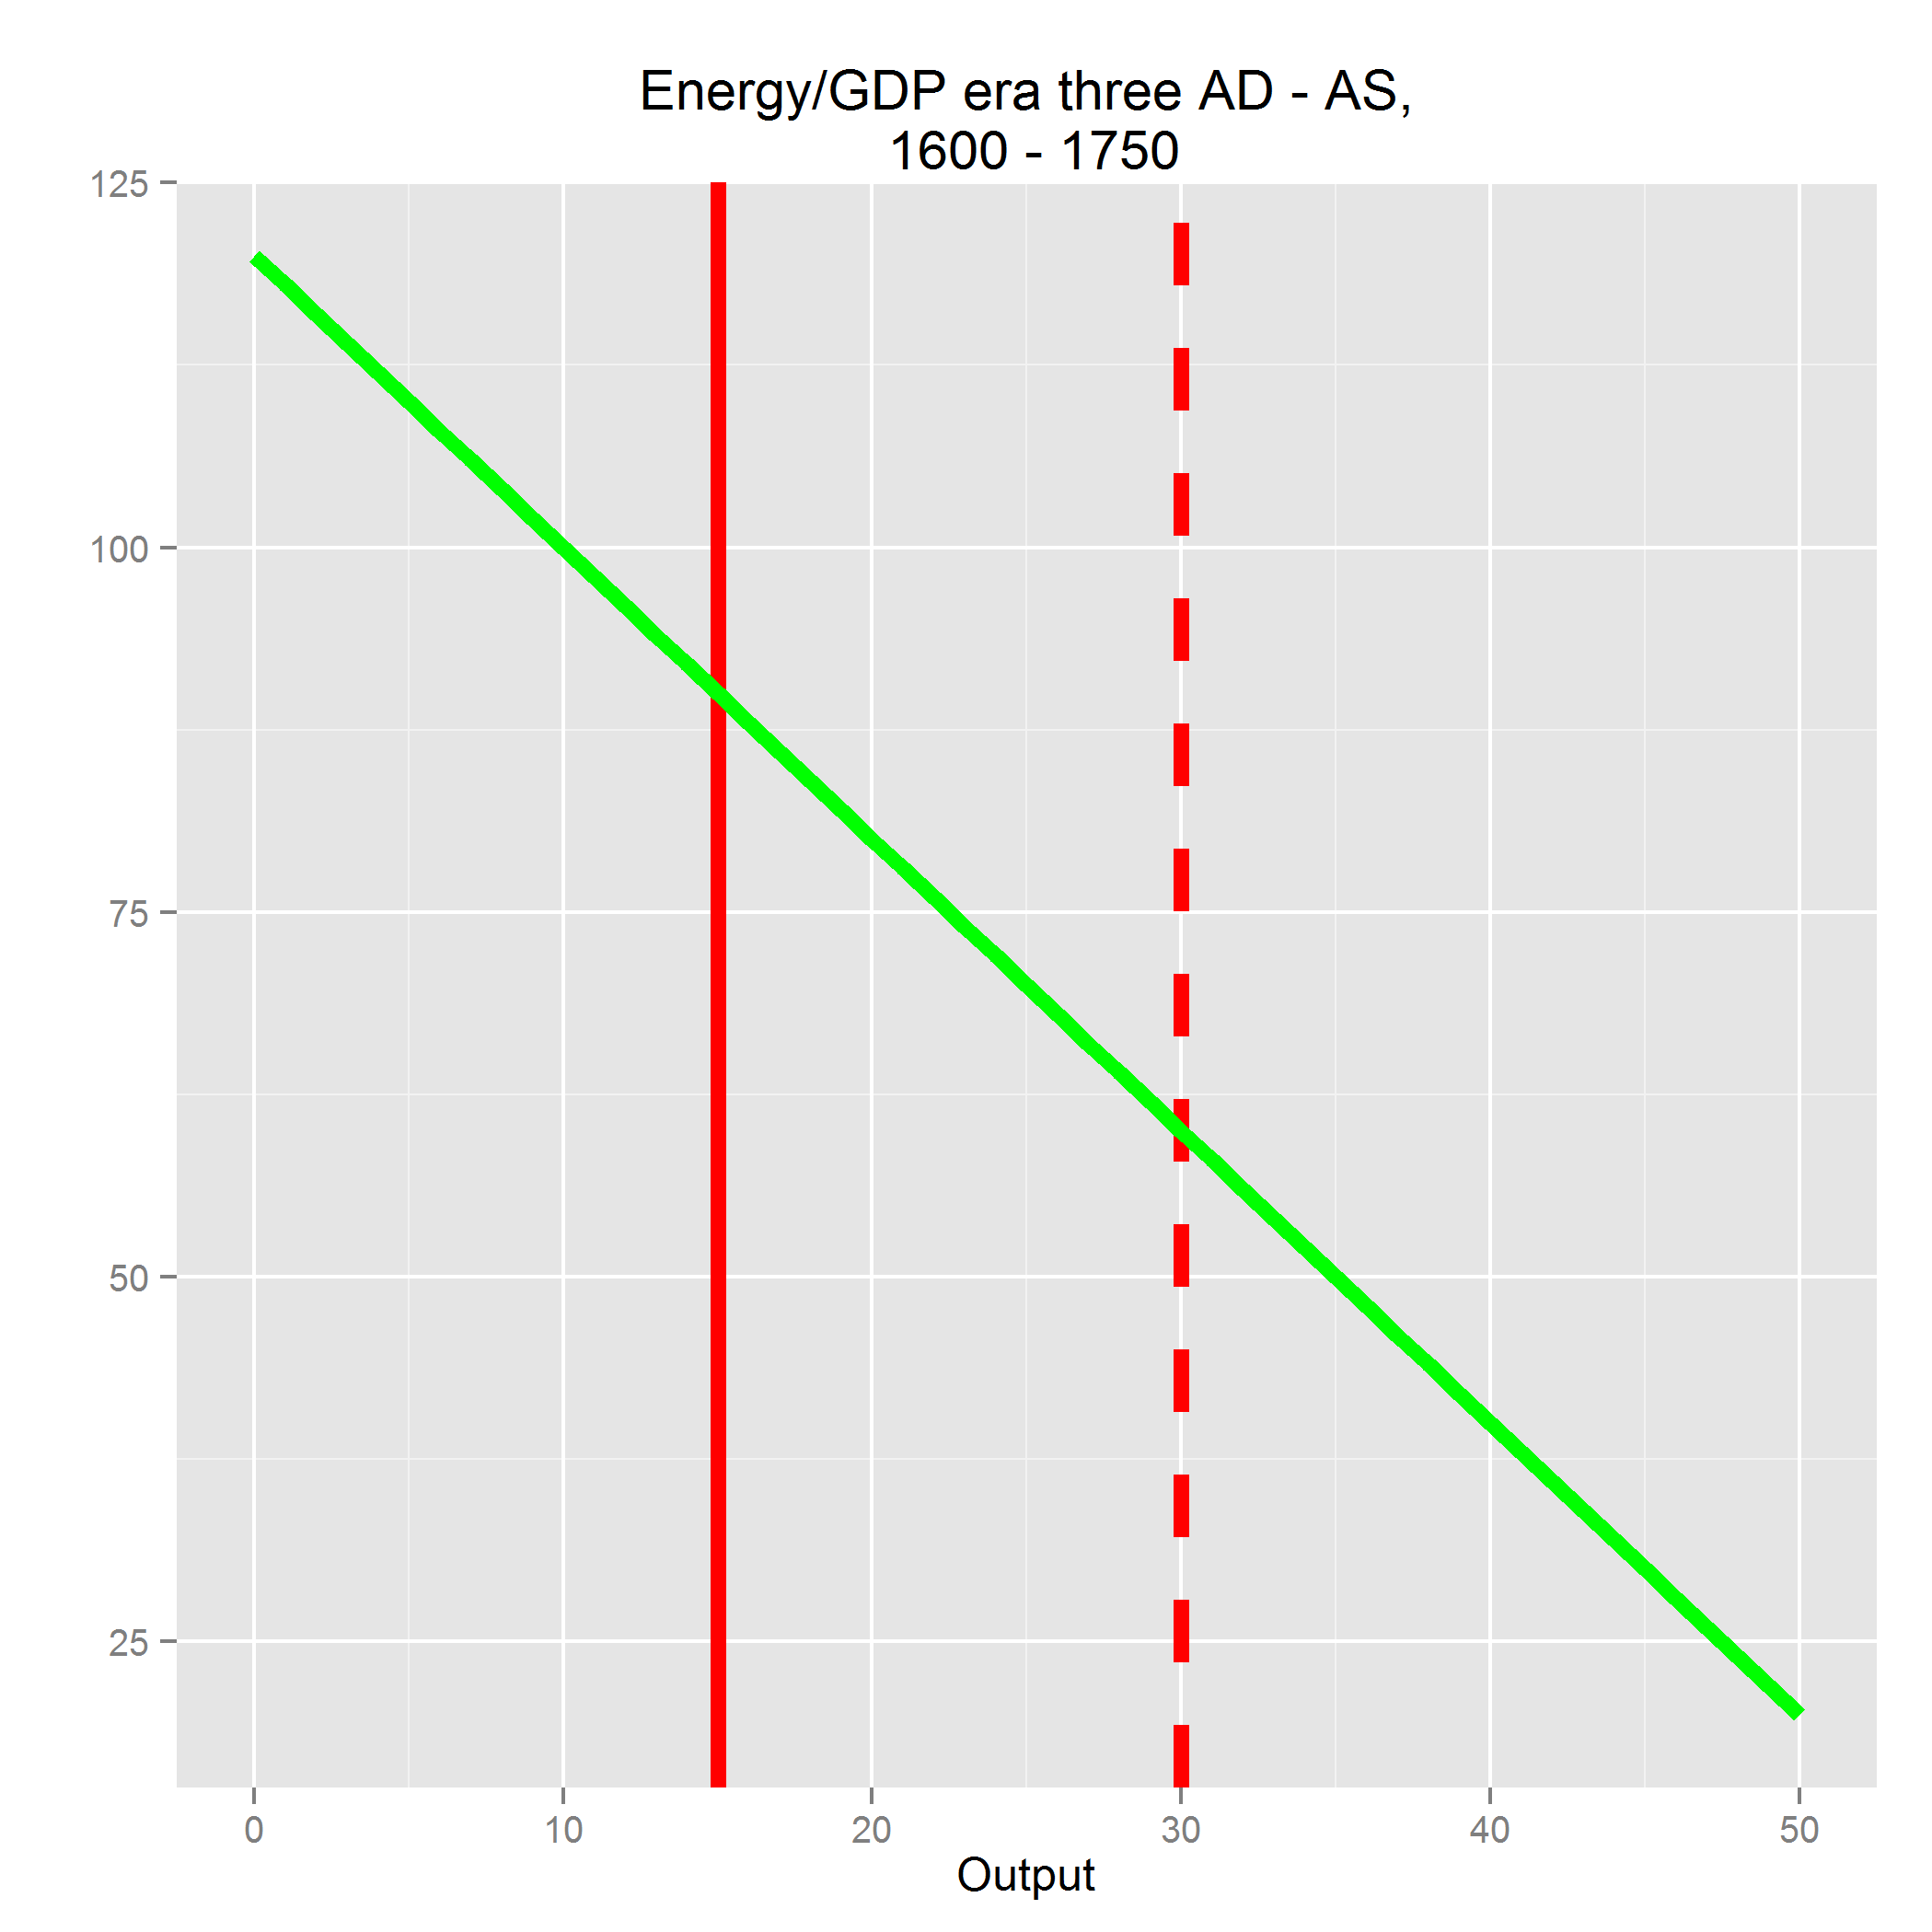
\includegraphics[width=0.25\textwidth]{era3}}
		\mbox{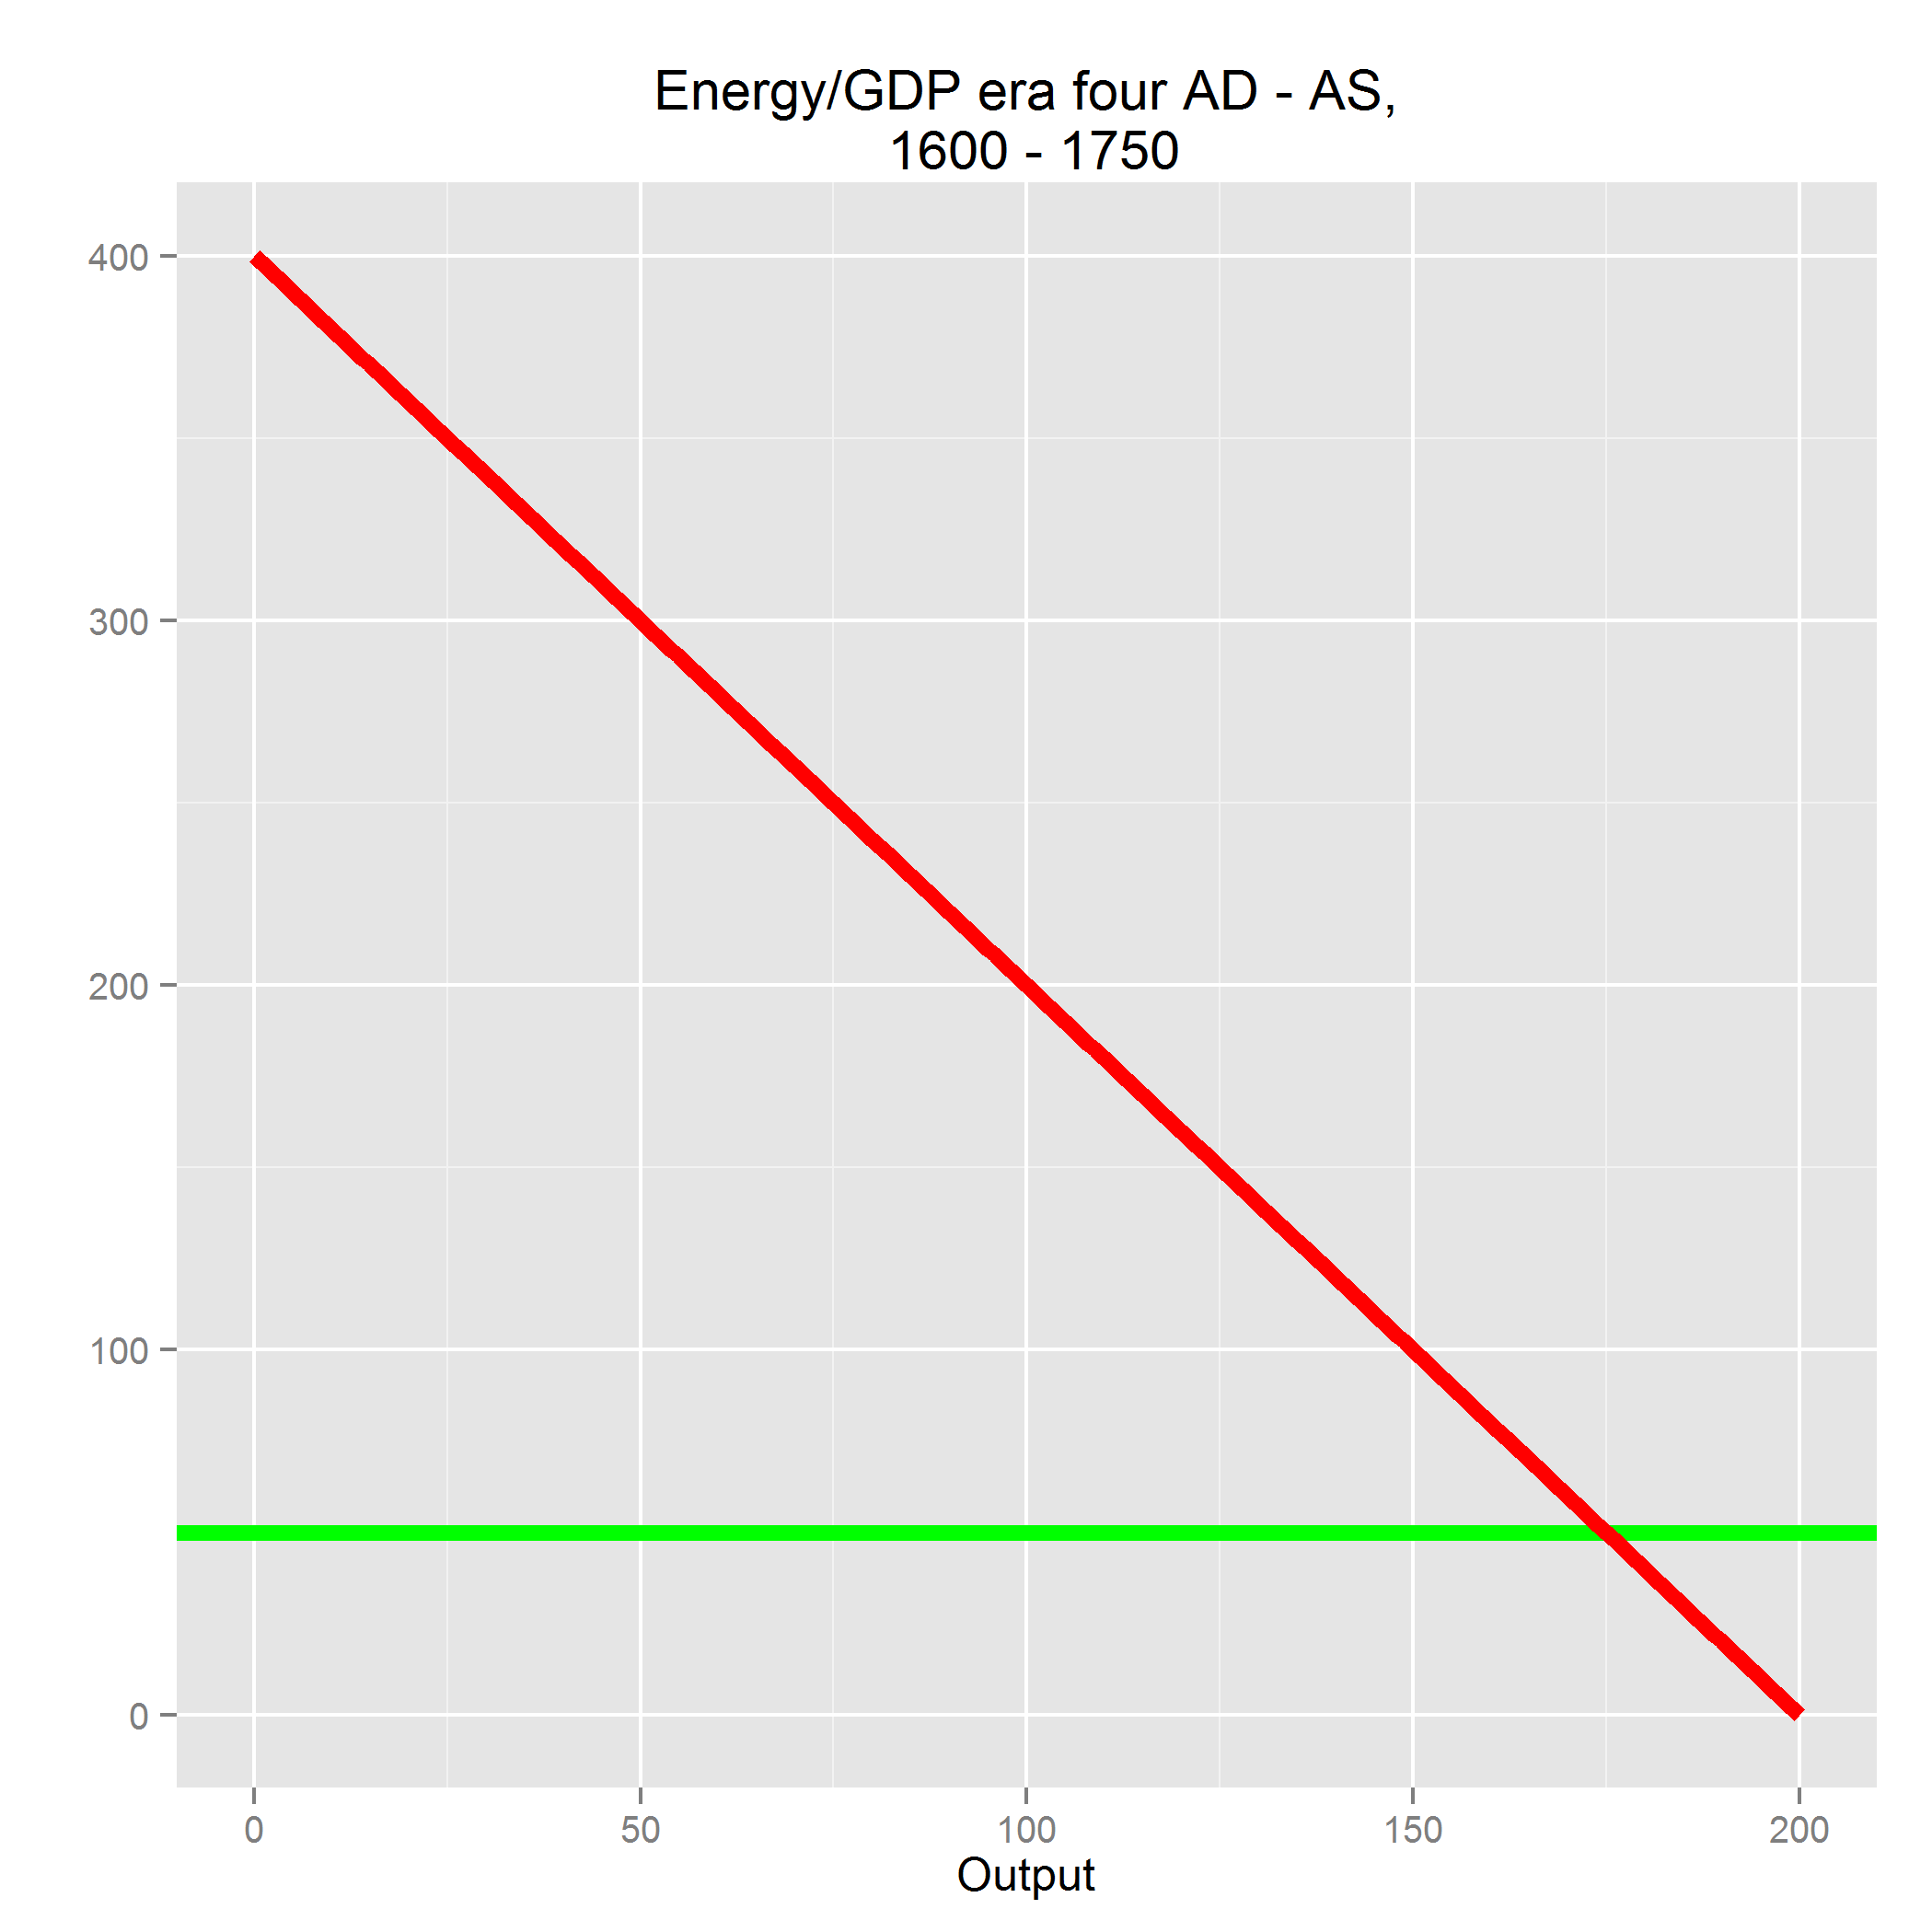
\includegraphics[width=0.25\textwidth]{era4}}				
		}
\end{figure}

\begin{figure}[h!]
		\caption{Desaguliers manuscript}
		\label{fig:desagulier}		
		\center
%		\mbox{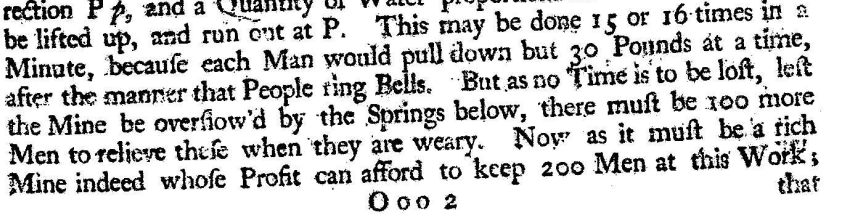
\includegraphics[width=0.95\textwidth]{desagulier1}}\\
%		\mbox{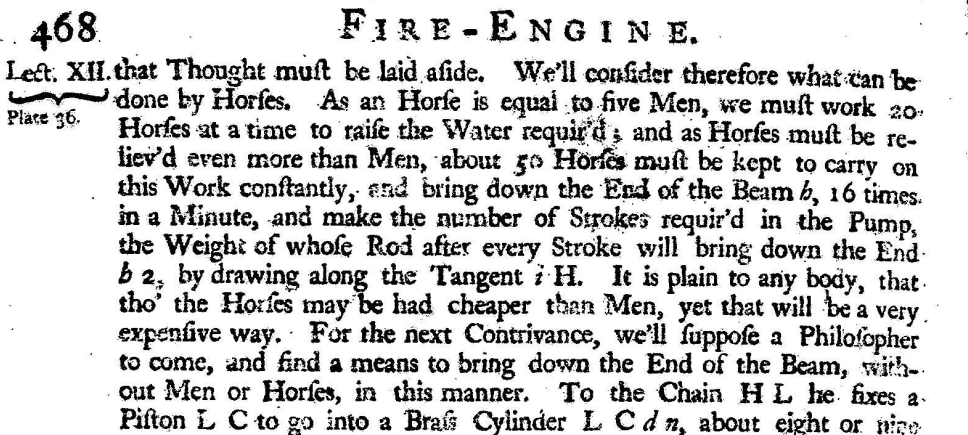
\includegraphics[width=0.95\textwidth]{desagulier2}}
		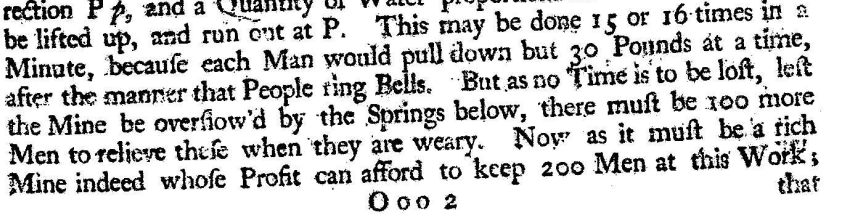
\includegraphics[width=0.95\textwidth]{desagulier1}\\
		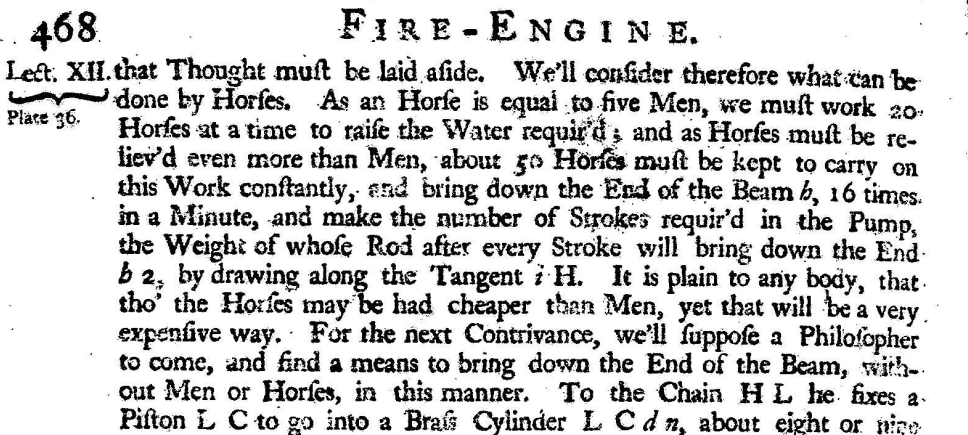
\includegraphics[width=1.05\textwidth]{desagulier2}
%		}
\end{figure}

\begin{figure}[h!]
\center
\caption{Real wage to energy ratios\\\textit{Source:} Robert Allen (2009)}
\label{fig:wage-energy}
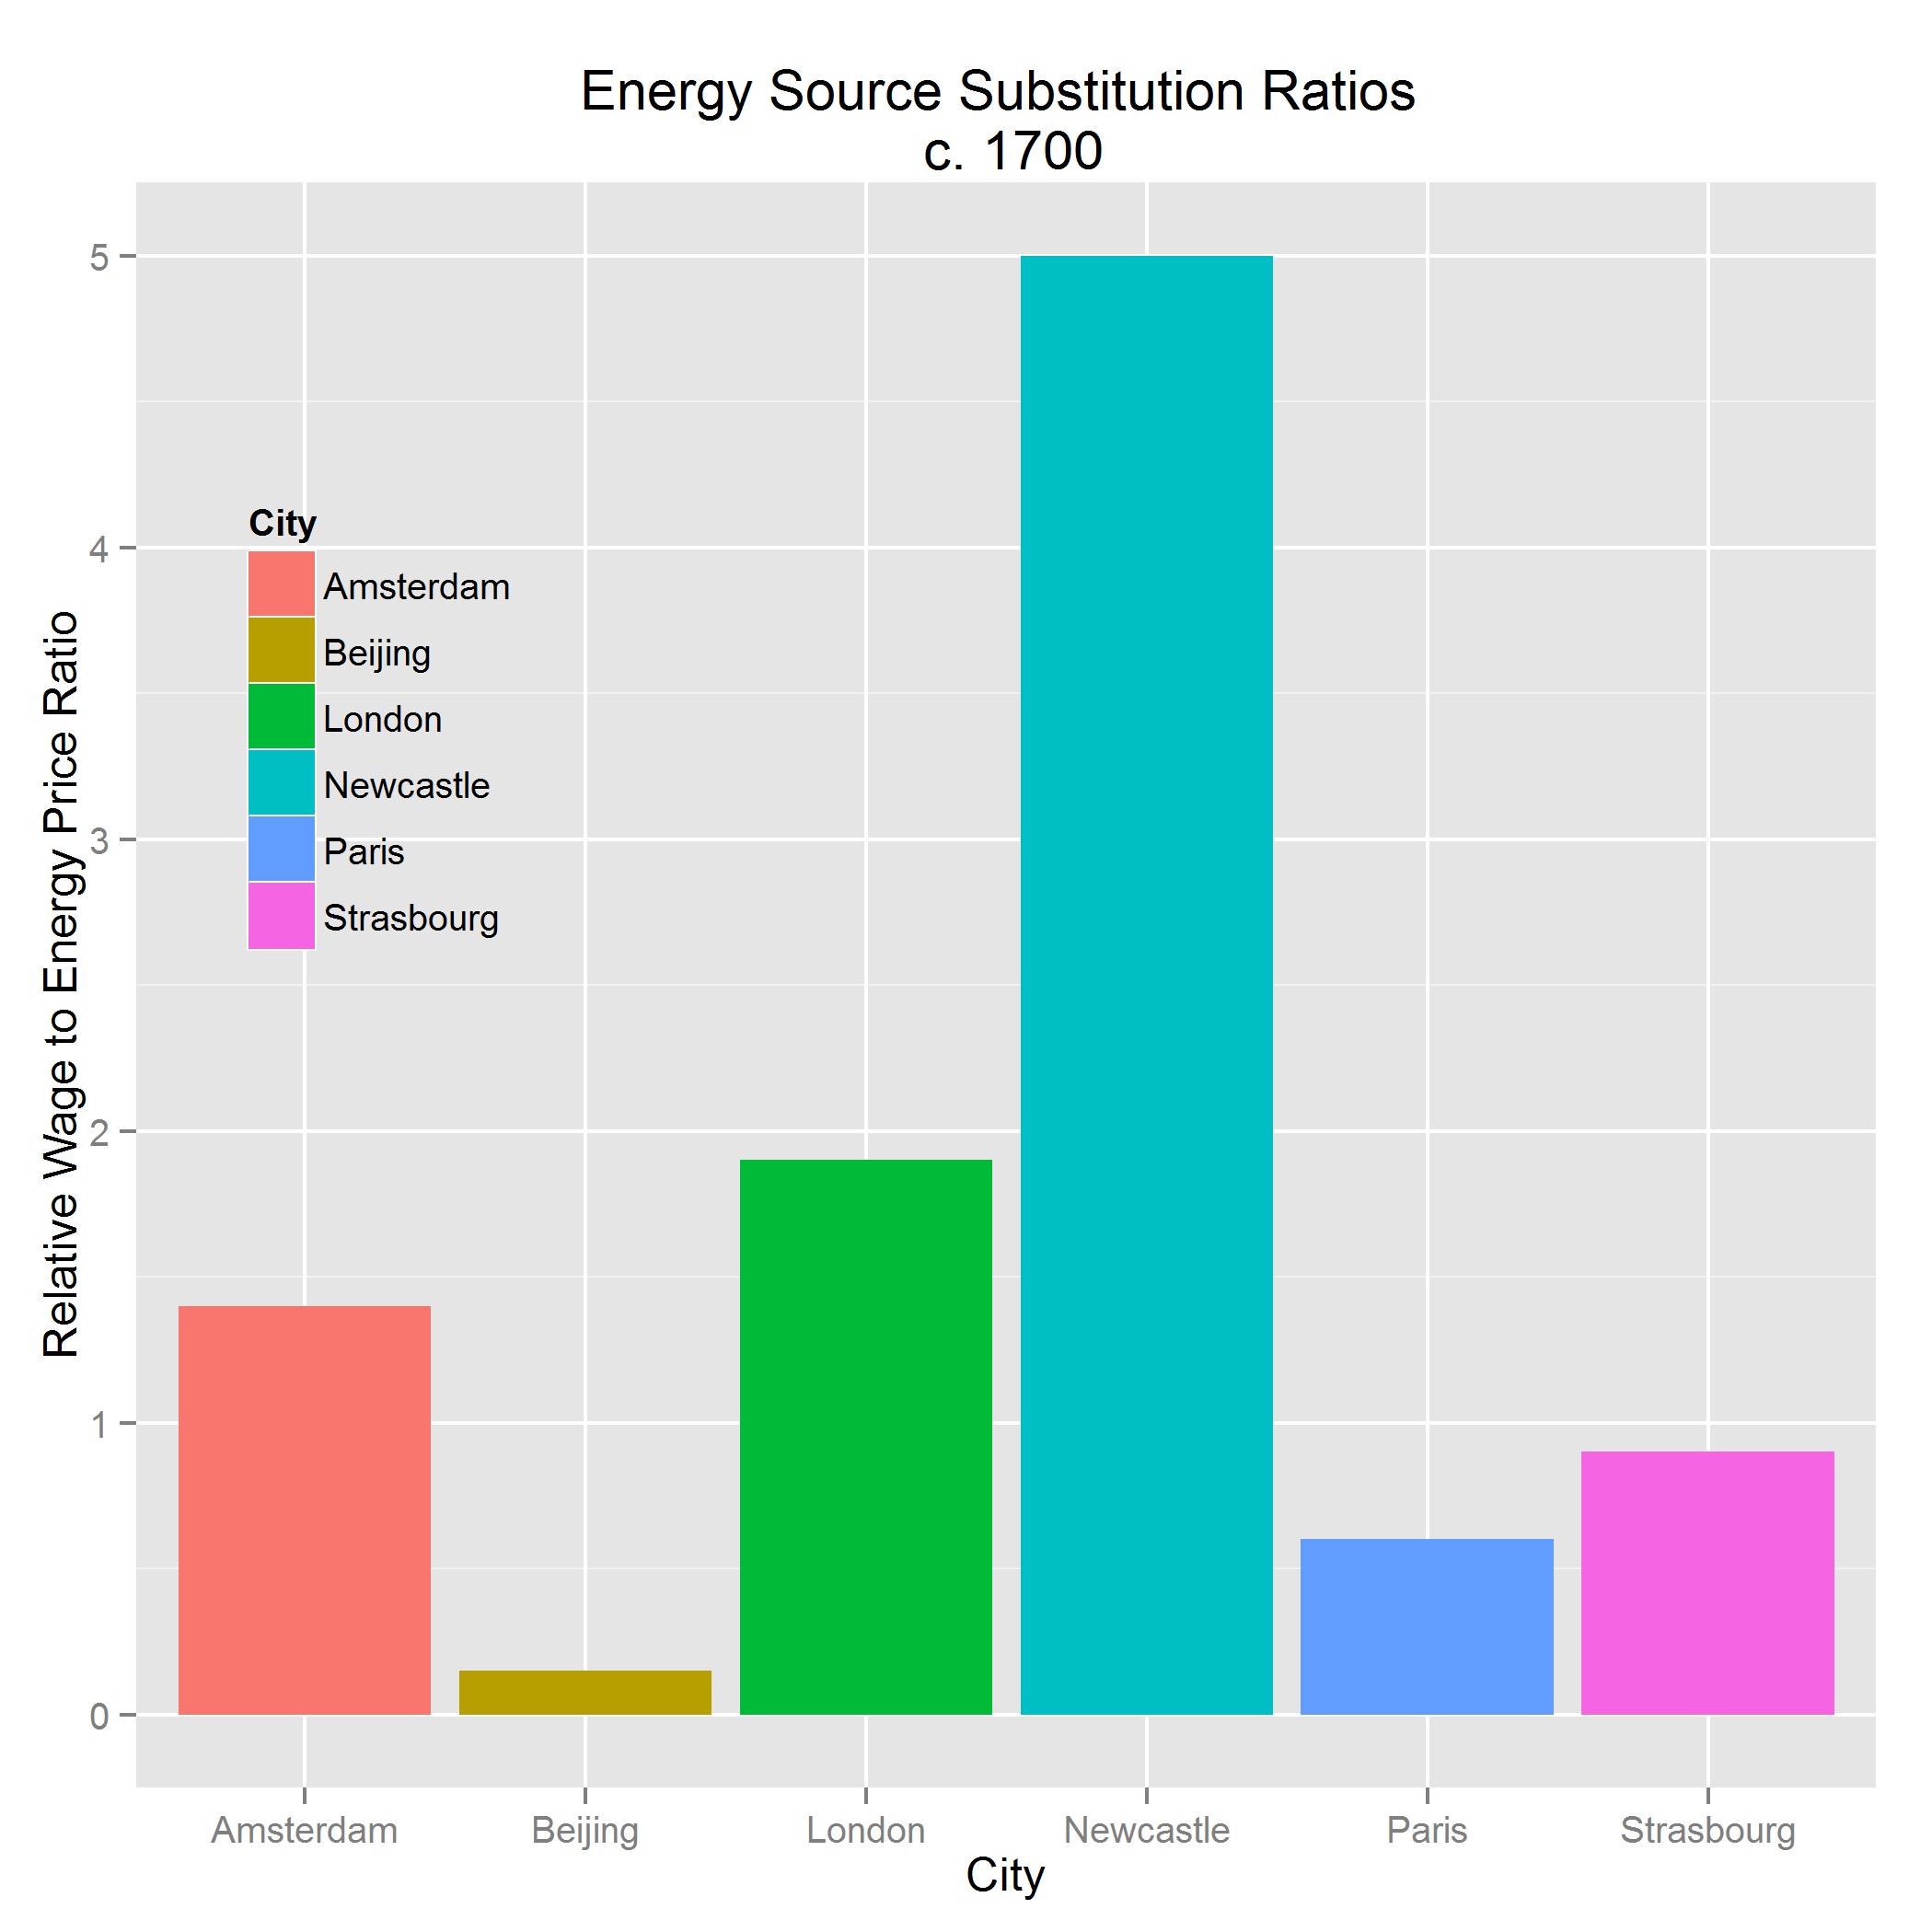
\includegraphics[width=0.9\textwidth]{wage-energy.png}
\end{figure}

\begin{figure}[h!]
\center
\caption{Standardized English energy intensity of GDP}
\label{fig:energyIntensity}
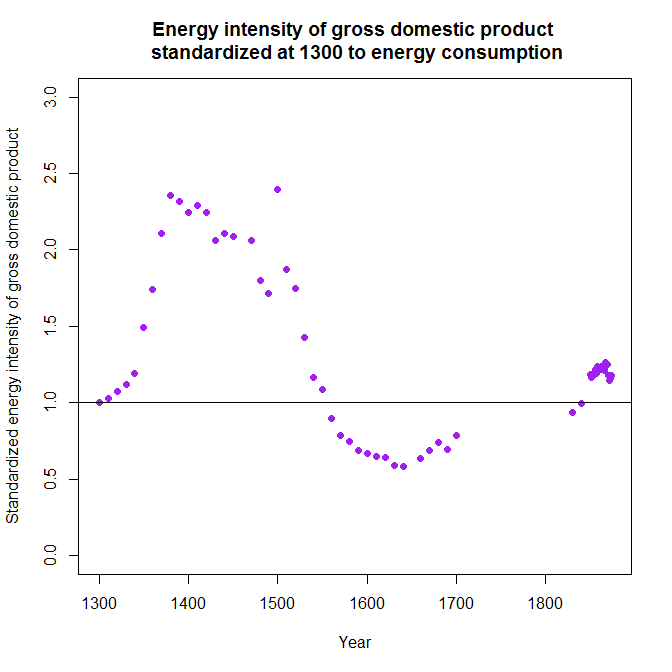
\includegraphics[width=0.9\textwidth]{energyIntensity}
\end{figure}

\begin{figure}[h!]
\center
\caption{Log of GDP, with structural breaks}
\label{fig:gbpgdplog.png}
\includegraphics[width=0.9\textwidth]{gbpgdplog.png}
\end{figure}

\newpage

\section{Equations}

		\begin{equation}
		\label{eq:mrp}
%		\frac{\text{Marginal Revenue Product}_{\text{ organic energy joule}}}{\text{Price}_{\text{ organic energy joule}}} = \frac{\text{Marginal Revenue Product}_{\text{ fossil energy joule}}}{\text{Price}_{\text{ fossil energy joule}}}
		\frac{\text{Marginal Product}_{\text{ organic energy joule}}}{\text{Price}_{\text{ organic energy joule}}} = \frac{\text{Marginal Product}_{\text{ fossil energy joule}}}{\text{Price}_{\text{ fossil energy joule}}}
		\end{equation}
		\myequations{Microeconomic theory - marginal product} 
		
%granger tests over at least two regimes
%add back in for full paper
%\section{Appendix A. Detailed Granger test output} 
%\label{app:Appendix A}

%\section{Appendix B. Time series analyses}
%\label{app:Appendix B}

\begin{comment}
\section{Appendix C. Future research}
survey on institutions/culture\\
empirical tests of institutional/cultural events\\
population curves\\
\label{app:Appendix C}
\end{comment}


\begin{comment}

\begin{verbatim}
> grangertest(per1eng ~ per1gdp,n)
Granger causality test

Model 1: per1eng ~ Lags(per1eng, 1:1) + Lags(per1gdp, 1:1)
Model 2: per1eng ~ Lags(per1eng, 1:1)
  Res.Df Df      F  Pr(>F)  
1     16                    
2     17 -1 8.3703 0.01059 *
---
Signif. codes:  0 �***' 0.001 �**' 0.01 �*' 0.05 �.' 0.1 � ' 1 
 grangertest(per1gdp ~ per1eng,n)
Granger causality test

Model 1: per1gdp ~ Lags(per1gdp, 1:1) + Lags(per1eng, 1:1)
Model 2: per1gdp ~ Lags(per1gdp, 1:1)
  Res.Df Df      F    Pr(>F)    
1     16                        
2     17 -1 21.772 0.0002582 ***
---
Signif. codes:  0 '***' 0.001 '**' 0.01 '*' 0.05 '.' 0.1 ' ' 1 
> grangertest(per2eng ~ per2gdp,n)
Granger causality test

Model 1: per2eng ~ Lags(per2eng, 1:1) + Lags(per2gdp, 1:1)
Model 2: per2eng ~ Lags(per2eng, 1:1)
  Res.Df Df      F Pr(>F)
1      7                 
2      8 -1 2.0643 0.1939
> grangertest(per2gdp ~ per2eng,n)
Granger causality test

Model 1: per2gdp ~ Lags(per2gdp, 1:1) + Lags(per2eng, 1:1)
Model 2: per2gdp ~ Lags(per2gdp, 1:1)
  Res.Df Df      F Pr(>F)
1      7                 
2      8 -1 0.2808 0.6126
> grangertest(per3eng ~ per3gdp,n)
Granger causality test

Model 1: per3eng ~ Lags(per3eng, 1:1) + Lags(per3gdp, 1:1)
Model 2: per3eng ~ Lags(per3eng, 1:1)
  Res.Df Df      F Pr(>F)
1      6                 
2      7 -1 1.0136 0.3529
> grangertest(per3gdp ~ per3eng,n)
Granger causality test

Model 1: per3gdp ~ Lags(per3gdp, 1:1) + Lags(per3eng, 1:1)
Model 2: per3gdp ~ Lags(per3gdp, 1:1)
  Res.Df Df      F Pr(>F)
1      6                 
2      7 -1 0.4703 0.5185
> grangertest(per4eng ~ per4gdp,n)
Granger causality test

Model 1: per4eng ~ Lags(per4eng, 1:1) + Lags(per4gdp, 1:1)
Model 2: per4eng ~ Lags(per4eng, 1:1)
  Res.Df Df      F   Pr(>F)   
1     22                      
2     23 -1 11.735 0.002418 **
---
Signif. codes:  0 '***' 0.001 '**' 0.01 '*' 0.05 '.' 0.1 ' ' 1 
> grangertest(per4gdp ~ per4eng,n)
Granger causality test

Model 1: per4gdp ~ Lags(per4gdp, 1:1) + Lags(per4eng, 1:1)
Model 2: per4gdp ~ Lags(per4gdp, 1:1)
  Res.Df Df      F Pr(>F)
1     22                 
2     23 -1 2.7737   0.11

\end{verbatim}
\end{comment}

\end{document}
\section{end}

\section{Defence proposal below here}
\newpage
			
	\section{Table of Contents}
	\tableofcontents
	\listoffigures
	\listoftables
	
	\newpage
	

	\section{The Research Question}
	
	The origins and causes of the English Industrial Revolution remain among economic history's most contested puzzles.  This slowly evolving revolution was likely the most important event in economic history since the \gls{neorev} approximately 10,000 years ago, and eclipses even that unquestionably cataclysmic transition in economic importance as measured by growth in per capita income.  Table \ref{tbl:gdpcapita} shows the growth in world per capita real income between CE 1 and 1900. \footnote{Data from Maddison 2007 \cite{maddison_world_2007}} Yet, even this primary outcome of the Industrial Revolution remains contested.
	
	In the first 17 centuries of the Current Era per capita output increased by about 32 percent, surely still hewing closely to subsistence.  By stark contrast, in the two hundred years between 1700 and 1900 world average per capita output increased by  over 100 percent.  If one considers the very narrow population base to which the increased income actually inured (about 15 percent of the 1900 world population, measured by nation-state, produced about 40 percent of world GDP), this is a remarkable outcome. The richest country in 1900, the United Kingdom, enjoyed per capita income of about 4,500 \gls{gkusd}, over three times the world average.
	
		\begin{table}[h!]
		\centering

%		\begin{adjustwidth}{-0.75in}{}

		\caption[World GDP per capita]{This table shows the growth of world GDP per capita in two periods covering almost two millennia. Maddsion's data, author's calculations. Dollars in 1900 Geary-Khamis International (US) Dollars}\label{tbl:gdpcapita}
		
		\begin{tabular}{lrr}
		\toprule
		Benchmark&GDP per capita,&Percent Increase\\
		Year&1990 G-K\$& from prior benchmark\\
		\midrule \midrule
		CE 1&467&-\\
		1700&615&31.7\%\\
		1900&1,261&105.0\%\\
		\bottomrule

		\end{tabular}
%		\end{adjustwidth}
		\end{table}
	
	In some respects, the English consumers and inventors between the reigns of \gls{lizIreign} and \gls{vicreign} forged a Faustian bargain with the future to achieve this miracle.  They almost surely did so unknowingly by unleashing a historically unprecedented positive feedback cycle of demand and production that has now lasted for 400 years; this event thus has the characteristic of an emergent macroeconomic effect.  %History also inserts great economic inequalities, instabilities and conflicts, environmental damages, and other existential threats into this record of unprecedented growth in incomes, surplus, and, thus, wealth for wide swaths of humanity.
	
	What happened?  How did it happen?  Why did it happen first in England when it did and nowhere else in accumulated history?  Why has it not regressed, as every known preceding surge in per capita income has done?  
	
	How should our understanding of this Revolution inform our understanding of economic development in the nation-states and global economy that followed England -- that is, how did the Revolution evolve and spread?  What can we learn about future economic development and growth?
	
	And very specifically, what role did effectively unconstrained rates of \gls{energy} play in the Revolution? What social and institutional changes help account for this ``miracle invention" by which the English for the first time in history, and uniquely at the beginning, ``escaped the constraints of an advanced organic society?" \footnote{Wrigley 2010, p. 239 \cite{wrigley_energy_2010}} In turn, what social and institutional changes did this revolution cause in England and the other economies which followed in her path?
	
	I consider whether this discovery--\textit{the ability to convert virtually unlimited energy to output through the macro-invention of industrial-scale machine-capitalism} \footnote{Eckel \textit{Coal, Iron, War}, 1921  \cite{eckel_coal_1921}}---is the real, although in significant senses accidental, invention of the Revolution.  If so, we must consider this history seriously as we gaze into the physical and economic future of our species and planet.

		\subsection{What is the Study About?}
		
			\subsubsection{Nature and significance}
			This study explores the role of energy consumption in \gls{growth} and development.  The research question arises as one views long-period time-series of both per capita output and per capita energy consumption.  Both can be best described visually as super-exponential growth curves; thus, it is natural to ask how they are related.  The characteristic shape is seen in Figure \ref{fig:road}.\footnote{Economist Magazine, December 23, 1999  \cite{_road_1999}}
			
			\begin{figure}
			\centering
			\caption[Road to riches hockey stick]{From a 1999 Economist magazine article, based on the Angus Maddison data, illustrating the ``hockey stick'' effect of per capita GDP growth in Europe. Usefully annotated with historical events}\label{fig:road}
			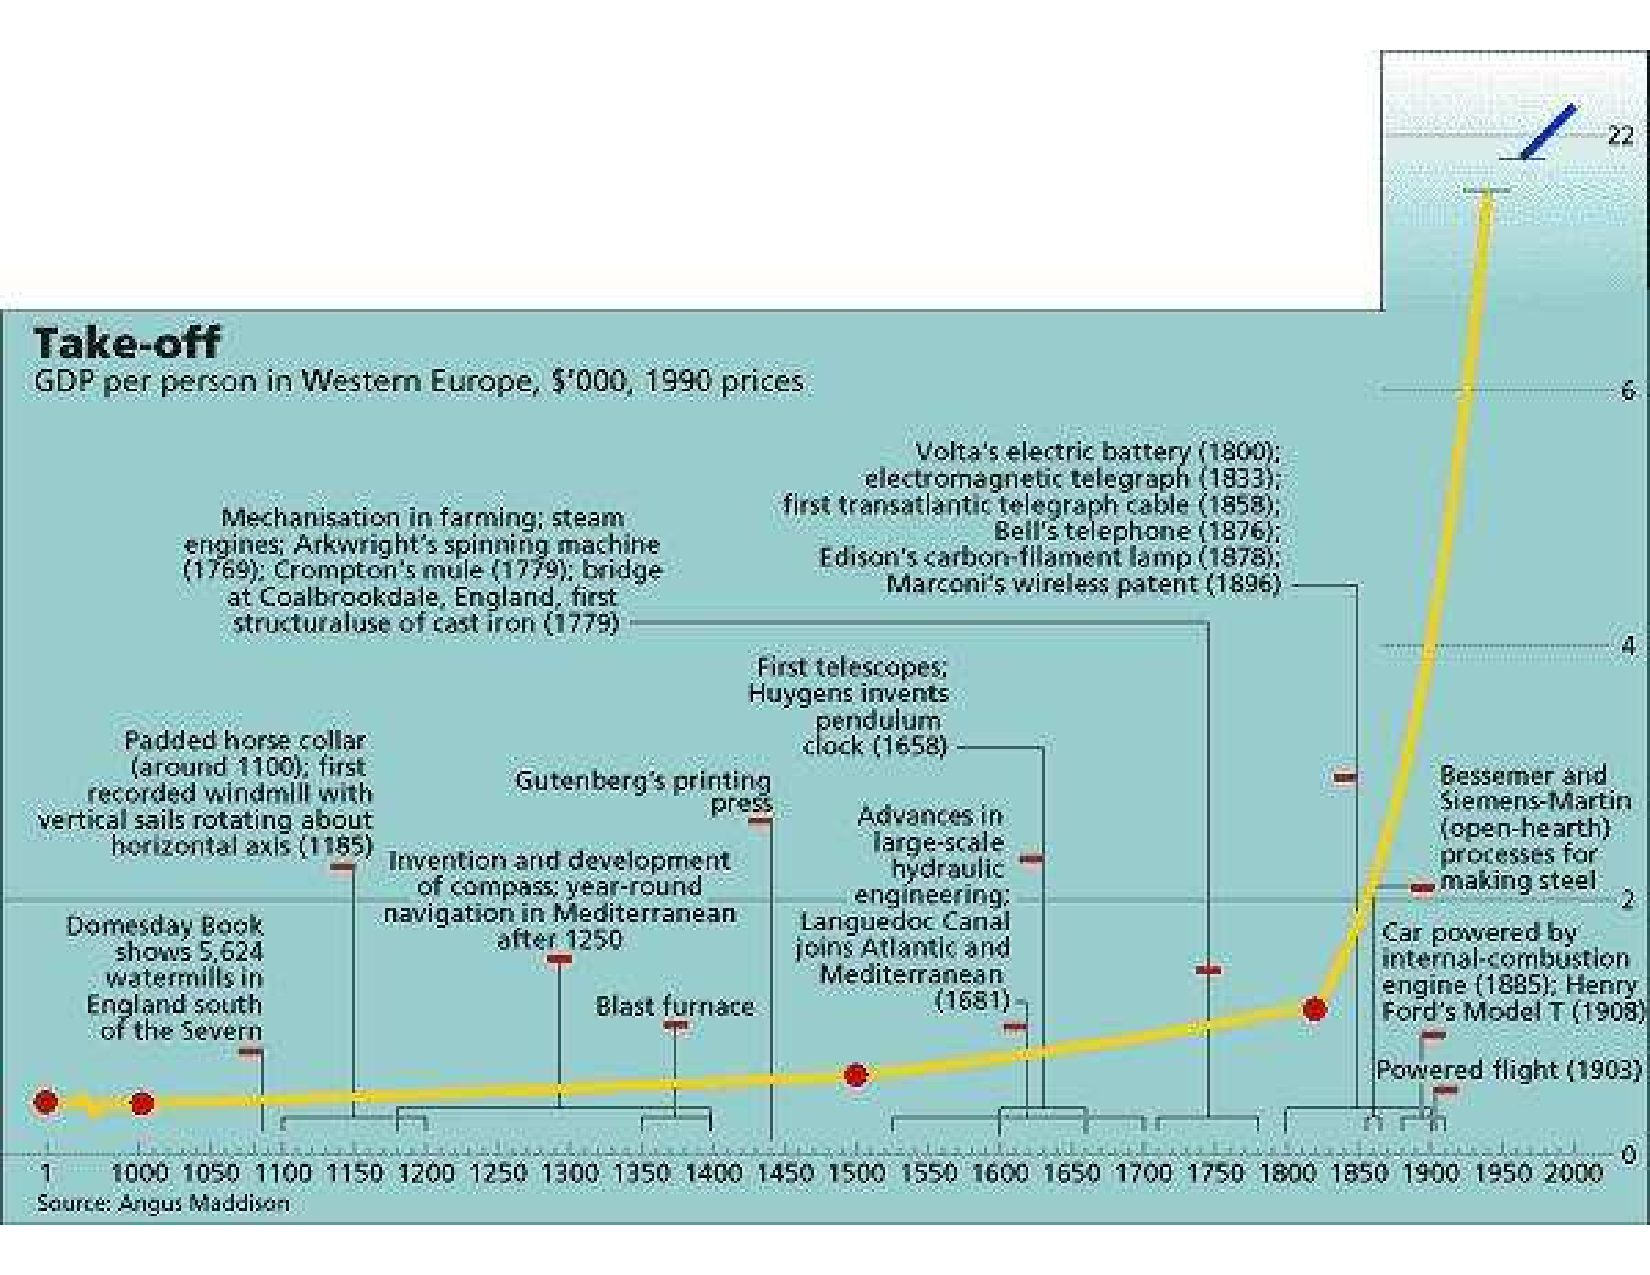
\includegraphics[width=0.8\textwidth]{../images/roadtoriches.pdf}
			\end{figure}
		
			A word on the title: Sir Arthur A. Lewis in his iconic 1954 ``Economic Development with unlimited supplies of labour'' \footnote{Lewis, 1954.\cite{lewis_economic_1954}} develops as a central theme that, in underdeveloped economies, labour will be used even if its marginal product is zero due to its relative abundance.
			
			I can construct similar examples in modern energy use; suppose I left the computer on which I am composing this unattended but on for several hours before writing this paragraph. It is not clear what the marginal product of that unattended energy consumption is: The computer did no writing or editing while I was absent. If I were writing by quill pen and candlelight, I would likely not have left the candle burning unattended due to fire risks and the high per lumen cost of medieval candles. The abundance of modern energy changes the expected marginal cost/marginal benefit equation.
			
			Another way to think about modern energy consumption is that the ratio of mineral energy available for whatever task, be it commodity manufacturing, service provision of various kinds including transportation, or writing a dissertation, is virtually unconstrained relative to the amount of the very largest amount of human energy I could possibly marshal for any of those tasks.
			
			So the title contextualizes the way in which I view modern energy consumption, and emphasizes how uniquely important the great English invention was.
			
			\subsubsection{Contributions of the study}
			\begin{enumerate}
			\item I clarify the historical explanation of this Revolution.  The explanation has fragmented over several economic generations into several ``camps" from which I hope to abstract what is both necessary and sufficient to explain the magical event. The story is complex, enriched with feed-back mechanisms, and clearly not mono-causal in the choices of supporting historical events.
			
			One can view the range of prior explanations of the English Industrial Revolution as a continuum from purely cultural to purely thermodynamic, with religious, cultural, social, institutional, technological, and geographical explanations arrayed along the line. By far, the most common explanations are weighted toward some form of English cultural exceptionalism. 
			
			\label{par:deirdre} Perhaps the most eloquent of this class is the recent series of books by Deirde McCloskey currently being published under the banner of the ``Bourgeois Era.''  Professor McCloskey details (in a promised six volumes) the great cultural changes that surrounded the English Industrial Revolution.  The series describes processes which are the antithesis of Marxian historical materialism. While there are many compelling stories in this history, this paper counters her thesis with a conviction that the actual story is, in fact and on the evidence, primarily a materialist story which caused and was supported by the evolving cultural and institutional environments. \footnote{The series currently consists of two published volumes, ``The Bourgeois Virtues'' (2007), and ``Bourgeois Dignity'' (2010) \cite{mccloskey_bourgeois_2010}}
			
			
			\item I propose a new definition of the English Industrial Revolution: a historically unique development that enabled the English macroeconomy to consume a virtually unconstrained amount of energy, and thus to escape any practical supply side limitation on output.  For perhaps the first time in history demand, not supply, became the limit of output; output growth exceeded population growth for an extended period of time.  Unprecedented growth of both macroeconomic productivity and \gls{surplus} accumulation became the new normal.
			
			\item Further, I explore my intuitions with the most analytically useful analysis I am aware of for this kind of problem.  Specifically, I  use the methodology of the so-called \gls{copenhagen} to investigate and attempt to explain the relationships and dynamics among energy consumption rates, output growth, and population growth. The method allows admitting exogenous events, so that if, for example, a statistical structural break appears in the data starting near the time of Gutenberg's invention, one can both recognize that in the model in a control sense and hypothesize that it was an important event. While the historically constructed series I use can surely be problematic, in a sense testing them with rigorous statistics could possibly highlight weaknesses in the construction methods.
			
			The method is capable of decomposing feedback loops into both short-run and long-run components.  To my knowledge, this decomposition method has never been attempted over long historical-period data sets.
			
			\item I apply the empirical methodology to two relatively new long-period histories of English energy consumption. One is from Roger Fouquet, \footnote{Fouquet's new study on English energy \cite{fouquet_heat_2008}} and one from Paul Warde. \footnote{Energy consumption from Warde's 2007 work. \cite{warde_energy_2007}} My strategy is to empirically test both inputs and compare the results both economically and statistically.
			
			\item As a future research agenda, 
			
			\begin{enumerate}
			
			\item I will extend this methodology to examine other economies in phases of significant growth; clearly the United States and China should be included, but any economy with sufficient historical data is a potential target. \label{par:china}
			
			\item I will use the empirical methods to decompose global growth over the period with available meaningful data.  
			
			\item Finally, I may consider an energy-based theory of income, growth, and wealth, and contrast that with extant micro-economic marginal productivity based theories including "new growth" New-Keynesian theories. If energy consumption is proven foundational to economic growth, then a measure of \gls{surplus} as energy consumption above \gls{bio} \footnote{Brad DeLong 1998. DeLong discusses GDP and population estimates, and uses this evocative term. \cite{delong_estimates_1998}} may prove interesting and useful.
			\end{enumerate}
			\end{enumerate}

		\subsection{Statement of the Research Question and Main Hypothesis}
		The research question asks how English energy consumption and economic output are structurally related, considering population levels, over a long period preceding and spanning the English Industrial Revolution.
		
		My main hypothesis is that learning to consume unconstrained energy was responsible, at least in the statistically causal sense, for the massive increases in per capita output first demonstrated in the English Industrial Revolution. Refer to Figure \ref{fig:road} and Table \ref{tbl:gdpcapitauk} for historical English per capita GDP growth.\footnote{Data from Maddison 2007 \cite{maddison_world_2007}}
		
		\begin{table} \centering
		\caption[UK GDP per capita]{This table shows the growth of English GDP per capita in two periods covering almost two millennia. Maddsion's data, author's calculations. Dollars in 1900 Geary-Khamis International (US) Dollars}\label{tbl:gdpcapitauk}.
				
		\begin{tabular}{lrr}
		\toprule
		Benchmark&UK GDP per capita,&Percent Increase\\
		Year&1990 G-K\$& from prior benchmark\\
		\midrule \midrule
		CE 1&400&-\\
		1700&1,250&212.5\%\\
		1900&4,492&259.4\%\\
		\bottomrule

		\end{tabular}
%		\end{adjustwidth}
		\end{table}
		
		Thus, an understanding of that event is crucial to understanding \gls{growth}.


		\subsection{Subsidiary Hypotheses}
		\begin{enumerate}
		\item While the primary and clear discovery of the English Industrial Revolution was the ability to consume unlimited energy at the level of the macro economy, there are a series of necessary social and institutional precursors. 
		
		These are in dispute, but I focus on identifying those that contributed to the incentives and skills of consuming unlimited energy. My initial candidates are the rise of consumer demand including (though at a later time) the export orientation of the English economy, and the accelerated accumulation and spread of knowledge after Gutenberg's \footnote{Johannes Gutenberg, 1398 - 1468, widely credited with inventing a printing press using mechanical moveable type} printing invention.
		
		Following Cottrell \footnote{W. F. Cottrell 1955 \cite{cottrell_energy_1955}} (and Karl Marx), there should also be testable hypotheses on the energy revolution causing social and institutional changes. This is an area for future research.
		
		\item While England clearly led, the revolution spread fairly quickly. I hypothesize that the structural dynamics of the early followers were similar to those of England.  Via the framework I am developing, this should be a testable hypothesis in future research.
		

		
		\item I further hypothesize that the rate of energy consumption is a much better predictor of \gls{surplus} than any other factor including ``capital'' and ``technical progress,'' as they would enter a common specification of the Solow macro production function.
		\end{enumerate}


  		\subsection{Limitations and Delimitations}
		
		In this proposal, the focus is on the English experience; I do extend the model to a global economy by testing specifications which admit English exports as support for growth in overall demand. In the research for this proposal, country comparisons arise and I reference them. As I continue this work, I will extend the methods to other key economies as described on page \pageref{par:china}.

		\subsubsection{Limitations}
		The primary limitation in the study is the accuracy of the data series since they are historically constructed by various economic historians.  I will evaluate several sources for the data and attempt to make a logical choice of which series I will use.  As questions arise on the accuracy, my considered response is ``what choice do we have?"  We should let the data tell us whether the model(s) using the series are credible statistically. Thus, doing the econometric analysis in this way may be peripherally useful to the historians who have been compiling this data, as it will suggest the validity of the data.
		
		\subsubsection{Delimitations}
		The primary delimitation that I have imposed is to use only three time series as core variables in the proposed study; Gross Domestic Product (GDP), energy consumption, and population are treated as endogenous variables. I will allow historical events suggested by structural breaks in these endogenous series to enter the model.  Depending on model fits, I may consider adding other theoretically justifiable series, for example, energy prices. This parsimonious ``simple to complex'' approach is the preferred methodology of the \gls{copenhagen}.
		
		I prefer to use Bayesian inference rather than classical methods for it's superior statistical characteristics. However, the applied methodology I need to deploy is not yet up to the challenge, so I will limit this study to classical inference.

		
	\section{Literature Review}
	There are two main bodies of literature that bear on my topic.  The first deals with the historical causes of the English Industrial Revolution, and the subsequent histories of the other countries which bear on their path to modern economic growth.
	
	The second body of literature deals with the econometric analysis of energy and modern economic growth.
	
	This study will both deal with the intersection of these bodies of literature, and extend them in the following ways:
	\begin{enumerate}
	\item Use econometric methods to fully describe the structural dynamics, both long- and short-run, relating economic growth and energy consumption.
	\item Identify the most important historical-institutional changes that led to modern economic growth as first experienced in the English Industrial Revolution.
	\item Since the prime cause of the English Industrial Revolution remains under debate, I will attempt to add to the debate based on the evidence.
	\end{enumerate}
	
	\subsection{Contributions of the core literature}

	\paragraph{Primarily cultural explanations of the English Industrial Revolution -- the English cultural exceptionalists.} In line with my metaphor of a continuum of primary reasons to explain why the Industrial Revolution was English and happened in the $18^{th}$ century, I first describe some of the more prominent cultural or institutional primacy authors. Note that almost all historians who approach this problem end up with multi-causal explanations, so this categorization is based on my judgement. 
	
	Deirdre McCloskey, who I referenced earlier, provides an acutely observed and detailed history of the cultural, social, and institutional changes that contributed to the Industrial Revolution. As is common among these scholars, coal gets a mention. In fact it gets a full chapter (22) in McCloskey's ``Bourgeois Dignity'', \footnote{McCloskey 2010 \cite{mccloskey_bourgeois_2010}} but is only one of very many factors (and chapters -- a total of 46) for McCloskey.
	
	David Landes, with his ``The Unbound Prometheus'', \footnote{Landes 1969 \cite{landes_unbound_1969}} became the mainstream doyen of recent documenters of the Industrial Revolution, and discusses in some detail the proximate technical and industrial institutional changes. While primarily a supply-side explanation, he does address the role of demand in leading technological change. He recognizes the role of energy substitution.  But in the end, he does not satisfactorily explain why England and why then without appealing later work to the theme of English cultural exceptionalism.
	
	Jack Goldstone perhaps epitomizes modern economic historians. Goldstone is a premier member of the ``California School'' of anti-Eurocentric revisionist historians, and a prolifically good one. He thus has the dual burden of explaining ``why England?'' and ``why not China?'' In the end, while at root a revisionist, he lands not that far from Landes. From ``The Rise of the West -- Or not,'' he states `` ...a very accidental combination of events in the late seventeenth century placed England on a peculiar path, leading to industrialization and constitutional democracy. These accidents included the compromise between the Anglican Church and Dissenters, and between Crown and Parliament, in the settlements of 1689; the adoption of Newtonian science as part of the cosmology of the Anglican Church and its spread to craftsmen and entrepreneurs throughout Britain; and the opportunity to apply the idea of the vacuum and mechanics to solve a particular technical problem: pumping water out of deep mine shafts in or near coal mines. Without these particular accidents of history, there is no reason to believe that Europe would have ever been more advanced than the leading Asian civilizations of the eighteenth and nineteenth centuries.'' \footnote{Goldstone 2000 \cite{goldstone_rise_2000}}
	
	So Goldstone asserts an accidental path-dependent institutional explanation while giving a brief hat tip to the development of steam engines. He is a self-described anti-Eurocentric California School member, but exposes the contradictions that this group faces. For example, he brackets the arguments of the intellectual space by ending up in a multi-causal culturally biased explanation that describes a great deal, but in the end explains little about primary causes that are prescriptively useful for development economists; and in my opinion he does not fully explain ``what happened,'' ``why it happened,'' and ``when it happened.'' He understands that the pumping machines for coal mines were important, but misses that it was the coal use itself that was the primary driver of the Industrial Revolution.
	
	Joel Mokyr is perhaps the premier purveyor of the view of the ``scientific-practical culture of England-the engineers, craftsmen, and entrepreneurs who specialized in applying the Newtonian science into machines useful for production.'' So he is the chronicler of the tinkerer class, (allegedly a quote of Peer Vries - for whom I am searching for a citation) the core of the English who were culturally uniquely capable of developing the technology of the Industrial Revolution. \footnote{Joel Mokyr 1992 \cite{mokyr_lever_1992}}
	
	It is not possible to conclude this far too abbreviated summary of Eurocentric historians without briefly mentioning Max Weber -- in important ways the most Eurocentric of all observers. While too reductionist in fact, what I take from Weber is that he essentially said that European protestant work ethics were the primary factors in the rise of the west. \footnote{ Max Weber, \textit{The Protestant Ethic} 2002(1904-1904,revised 1920) (\cite{weber_protestant_2002}}


	\paragraph{Somewhat cultural explanations of the English Industrial Revolution.}  
	This group of Economic historians is smaller than the first group because in my judgement they have developed a more coherent view of the English Industrial Revolution. It is worth noting that the first group (excepting Weber) are all American historians. This group is only partly American and is not Eurocentric. Kenneth Pomeranz is American. Robert Allen is also, but works professionally in England. Carlo Cippola was Italian who later in his career taught at Berkeley. It is Cipolla with whom I start.
	
	Carlo Cipolla had a unique perch from which to develop his worldview -- from Pavia west of Venice, thus astride the great medieval land trade routes and geographically centered on the land of the Italian city states, he could see and think both to the west and east. His wry and witty histories are the antecedents of Mokyr and later historians in the sense of describing the technical advances of the European adventure, but within the context of a world historian.

	One of his most acute set of observations, in his 1966 ``Guns, Sails and Empire,'' \footnote{Cipolla 1966 \cite{cipolla_guns_1966}} describes the new technology of early modern era European sailing ships as an energy revolution that ``transcended the limitations of human energy and obtained a decisive advantage over non-Europeans'' who were still using oarsmen and armed boarding parties. The far more energy intensive European war ships carried heavy cannon, yet could both out-run, out-manoeuvre, and out-fight their rivals. The Europeans, first the Spanish and Portuguese, then the Dutch, and finally the English used this highly energy-intensive technology to conquer and dominate the world's ocean trade routes and trade with a potent blend of military mercantilism. 
	
	Thus, while not ignoring cultural differences, Cipolla for me defines the true essential elements of the successful rise of the west by describing the first major energy revolution since the Neolithic, and prefiguring the $18^{th}$ century mineral energy revolution that was yet to come.

						
	California School stalwart Kenneth Pomeranz describes the crucial determinants in the rise of the west in terms of coal, colonies and cotton. As an anti-Eurocentric and sinologist, he describes fully the cultural and social similarities and differences between England and the most relevant Chinese comparable region, the Yangze Valley, and concludes that since the differences were not sufficient causes, the ``Great Divergence'' in the outcome must be instead explained through coal, colonies and cotton (as a substitute for English land-intensive wool). \footnote{Pomeranz 2001 \cite{pomeranz_great_2001}}
	
	Robert Allen uses a largely quantitative microeconomic approach to explaining the English Industrial Revolution. He even attempts an econometrically estimated theoretical model which includes some institutional variables. And in the end he comes close to my hypothesized truth, concluding that ``The British were simply luckier in their geology...there was only one route to the twentieth century -- and it traversed northern Britain''. \footnote{Allen 2009 \cite{allen_british_2009}}
	
	\paragraph{Primarily energetic explanations of the English Industrial Revolution.} The reference count reduces as we traverse the continuum. My primary references here are only two: Edward Anthony (E. A.) Wrigley, the great English economic demographer, and the little known Fred Cottrell. I also cite a couple of Dutch economic historians who for me complete the story of the English geological exceptionalism that Allen and Pomernz describe. Tony Wrigley strays from his demography ``day job'' into the fray as explainer of the English Industrial Revolution starting with his 1988 ``Continuity, chance and change: the character of the industrial revolution in England'' \footnote{E. A. Wrigley 1988, \cite{wrigley_continuity_1988}} in which he clearly lays out the prime cause as the transition from an ``organic'' economy, albeit an advanced one harvesting energy from \gls{insolation}, to a mineral economy in which the limitations of organic energy sources were transcended.
	
	In his 2010 ``Energy and the English Industrial Revolution'' \footnote{Wrigley 2010 \cite{wrigley_energy_2010}} he advances and summarizes his arguments and focuses on the advances in productivity from the mineral energy transition. Wrigley cites and builds on the much less known and highly contrarian work of the iconoclastic American sociologist Fred Cottrell, who thought deeply about the role of energy in human history.
	
	Cottrell wrote ``Energy and Society'' in 1955. \footnote{Cottrell 1955 \cite{cottrell_energy_1955}} A sociologist, he clearly had a significant background in economics. This foundational book describes human activity, including economic activity, in terms of its net energy requirements. The expansion of civilization and its standard of living is directly related to increasing access to energy supplies with an expanding net surplus of available energy output over what is required to harvest the energy, a term now called Energy Return on Investment (EROI).\footnote{A term dating to 1984 and attributed to Charles A. S. Hall, cf. \cite{cleveland_energy_1984}} The greater the energy surplus, the more the society can use energy for uses other than just extracting energy. So the wealth of nations becomes a function of their net energy surpluses.
	
	Cottrell provides interesting examples of net energy calculations, including the great increase in energy surplus from the transition to early modern European sailing ships, a topic to which Carlo Cippola returned a decade later. While discussing economic activity he does not use the term ``capital'' but rather the concept of high energy intensive ``converters'' (i.e. industrial machines). This he naturally contrasts with low energy intensity converters (man and other animals).
	
	Even while his approach is very close to that of the thermodynamicists, and usefully for this study, Cottrell uniquely and strongly asserts that changes in access to energy surpluses shapes civilization, its institutions, its social relations, and its culture. His causality runs from energy access to culture at the sociological level rather than the other way around as argued at least implicitly by many of the references here. The concept has lately been anointed ``sociological thermodynamics.''
	
	Finally for this group of energy-biased scholars, I cite two Dutch economic historians. Jan Luiten van Zanden is probably closest to a new institutionalist, and his recent compendium ``The Long Road to the Industrial Revolution: The European economy in a global perspective, 1000-1800'' \cite{van_zanden_long_2009} largely covers the institutional changes in north west Europe that preceded the English Industrial Revolution, changes such as the European Marriage Pattern to which can be attributed the Middle Ages' rise in incomes and consumption that set the stage for the demand-led revolution. 
	
	Additionally however, van Zanden discusses the Dutch growth experience and it is that experience that is fundamental to understanding how geographically privileged the English were in the following sense: the Dutch had essentially everything from a social, cultural, institutional and entrepreneurial standpoint that the English had. They attempted to move from a pre-industrial regime to an industrial one by using their only readily available energy source -- peat. They were successful until the peat ran out -- and the abundantly coal-fueled English prevailed. This experience is in essence a natural experiment that negates the arguments that the revolution was culturally driven.
	
	Prefiguring van Zanden in 1978, J. W. de Zeeuw's article ``Peat and the Dutch Golden Age'' \footnote{de Zeeus 1978 \cite{de_zeeuw_peat_1978}} directly attributes the Republic's economic rise to energy consumption, and provides economy-wide energy consumption calculations, including comparisons with other economies, giving empirical support to van Zanden's assertion.

	\paragraph{Thermodynamic explanations of growth.} There is a vanishingly small group of scholars who describe economic activity almost exclusively in thermodynamic terms. It is worth reflecting that from this standpoint all work, including all economic work, is a function of an energy transformation. Energy input causes output. A rare case of clear physical causality in economics -- thermodynamics does after all rule.
	
	The most well known thermodynamicist is the renowned mathematician and economist Nicolas Georgescu-Roegen. Georgescu-Roegen tied the second law of thermodynamics to production theory, pointed out the implications for the sustainability of economic growth, and thus laid the foundation for the modern fields of ecological and evolutionary economics. Ironically, his work has had little impact in the field of development economics. \footnote{Georgescu-Roegen 1975 \cite{georgescu-roegen_energy_1975}}
	
	More recently, Ayres et al. \footnote{Robert Ayres et al. 2003 \cite{ayres_exergy_2003}} have taken a microeconomic approach, using various production functions to empirically estimate coefficients on energy as well as labor and capital. They conclude that energy input is sufficient to explain away the infamous ``Solow residual'' that underpins modern growth theory, and in fact finding that one can drop both the labour and capital inputs, with energy input explaining most of the output. %\textit{Pace} Karl Marx. removed 10/13/11 per Garrett
	
	Much more recently, the compelling thermodynamic description of economic activity attracted a physical scientist, Timothy Garrett, who has modelled economic activity as a thermodynamic system and estimated the coefficient, and thus advanced Georgescu-Roegen's work on (the lack of) carbon-fueled output sustainability by simplifying the sometimes arcane calculations of carbon dioxide output. \footnote{ Timothy Garrett 2009 \cite{garrett_are_2009}} Garrett removes labour from the ouput estimation model, showing that value equals the rate of energy consumption with an estimate of $9.7 \pm 0.3$ Mw per 1990 USD.
		
	\paragraph{A brief summing up.}	Before reviewing the empirical methodology literature, a summary of the lines of thought discussed to date may be useful. What is clear is that the prime causes of economic growth and development are a much debated and unsettled topic. I have modelled that by the notion of a continuum of views with the ``culturalists'' on one end and the ``thermodynamicists'' on the other. The culturalists are by far in the majority, while the thermodynamicists are unquestionably correct at the physical level. 
	
	What the science needs to try to unpack are the important dimensions of the emergent social systems in which the thermodynamics operate, and according to Cottrell, which are largely a function of societies seeking a high energy surplus. By important, I mean those necessary social changes without which high energy surplus societies will not emerge. After all, the answer to why do some societies develop and others do not remains one of the great remaining mysteries of economics, and at least one key to unlock the mystery seems to be in a measure of energy surplus.
	
	Thus the empirical methodology becomes important. In general, there are two options: deductive theoretical models or inductive empirical models. In reality, one cannot inductively model without some notion of a theory. Would Newton have inferred gravity without the apple falling from the tree? Surely one's starting position is a matter of philosophy -- theory first or data first, not theory only or data only. One must at some point specify and test a model, or at least select the variables about which one wishes to speculate; theory is eventually implicit in those acts. My proposed methodology, data first, is guided initially by Christopher Sims, and fleshed out by S\o ern Johansen and Katarina Juselius. I briefly review that literature as well as an empirical survey by James Payne.
	
	\paragraph{Empirical methodology.} Christopher Sims' 1980 attack on the deductive methodologies which yielded the large system-of-equations models common after the Cowles commission work has reverberated through econometrics every since. Sims essentially said that the methods of restricting the systems-of-equations so that they were uniquely soluble were ``incredible'' by which he strongly implied ``impossible.'' \footnote{Sims \textit{Macroeconomics and Reality}, 1980 \cite{sims_macroeconomics_1980}} 
	
	Sims' core point is that systems-of-equations models require the modeller to make \textit{a priori} model (coefficient) restrictions which are theoretically unsupportable, in fact so many restrictions ($m^2$ in a reduced-form system of $m$ equations) that it becomes impossible to model with consistent theory. He further offered the ``solution'' of unrestricted \gls{var} which make no \textit{a priori} coefficient restrictions and, initially, no theoretical limits.
	
	Building on his work, and the cointegration work of Engle and Granger, \footnote{Granger 1986 \cite{granger_developments_1986}} Johansen and Juselius developed the \gls{copenhagen} some methods of which have been econometrically popular since the 1990's. \footnote{Johansen \textit{Likelihood-based Inference on Cointegration if the Vector Autoregressive Model} \cite{johansen_likelihood-based_1995}} The applied methodology is summarized in Juselius' 2007 book ``The Cointegrated {VAR} Model: Methodology and Applications'' \footnote{Juselius 2007 \cite{juselius_cointegrated_2007}} which is the analytic strategy I follow as described in section \ref{sec:genmethod}. To my knowledge, this method has not been applied in the type of historical context I propose to study.
	
	
	In his 2010 ``Survey of the International Evidence on the Causal Relationship between Energy Consumption and Growth'' \footnote{Payne 2010 , p. 86 \cite{payne_survey_2010}} James Payne concludes that the 101 recent studies he surveys yield no consensus of the relationship even at the country level. He attributes this failure to several methodological issues, one of which is not paying sufficient attention to the coefficients the various methods yield. 
	
	Payne's survey validates my choice of \gls{var} as a modelling strategy for my research question, and his criticisms of existing work validates my choice of using the \gls{copenhagen} methodology. According to Payne, the current researchers, in order to fully understand the causal relationship, must ``examine the coefficients with respect to both the sign (positive or negative) and magnitude of the relationship between energy consumption and economic growth.'' 
	
	None of the surveyed studies apparently use the full Copenhagen methodology which I will apply, and which should satisfy the methodological issues Payne identifies. None of these studies appear to attempt to model exogenous time intervention variables which, as I demonstrate in table \ref{tbl:station}, can make a significant difference in model specification. Further, the Copenhagen methodology maximizes the information extracted from the empirical model by decomposing short-, medium-, and long-run dynamics, little of which was reported in the surveyed works.
	
	While I hypothesize energy consumption as fundamental to economic growth, the short run dynamics of an economy learning how to consume energy at an unconstrained rate should provide insights useful for development economists.
	

	\subsection{Categorical Enumeration of Literature and Sources}

	Table \ref{tbl:cite} categorizes all the references considered during preparation for this topic defense; there will be additions and deletions in the final dissertation.
	\setlength{\LTleft}{-0.50 in}

	\begin{longtable}{llll} 

	\caption[Categorized references]{References categorized by function, school of thought, geographical coverage, and author \label{tbl:cite}}\\ 
		\hline\hline
	Historical, Empirical,&School of Thought&Country&Citation\\
	Theoretical, or Data&&&\\
	\hline\hline\hline
	\endhead
%%%%%%%%%%%%%%%%%%% Historical	
	Historical&Culture, Institutions&World System&Janet Abu-Lughod\cite{abu-lughod_before_1991}\\
	
	&Culture, Institutions&China&Rhea C. Blue\cite{blue_argumentation_1948}\\

	&Culture, Institutions&England&Coleman and Cuthbert \cite{coleman_economy_1977}\\

	&Culture, Institutions&U.S.&Davis et al. \cite{davis_american_1972}\\

	&Culture, Institutions&England, Holland&Jan de Vries \cite{de_vries_industrial_1994}\\

	&Culture, Institutions&England&Jack Goldstone\\
	&&&\cite{goldstone_why_2008,goldstone_whose_2000,goldstone_rise_2000, goldstone_capitalist_1983, goldstone_cultural_1987, goldstone_trend_1993, goldstone_initial_1998, goldstone_efflorescences_2002}\\

	&Culture, Institutions&England&Floud and McCloskey \cite{floud_economic_1994}\\
	
	&Culture, Institutions&World System&Andre Gunder Frank \cite{frank_reorient:_1998}\\
	
	&Culture, Institutions&China&Robert Hartwell \cite{hartwell_revolution_1962, hartwell_markets_1966, hartwell_cycle_1967}\\
	
	&Culture, Institutions&Multi-Country&William McNeill \cite{mcneill_rise_1963,mcneill_rise_1990}\\

	&Culture, Institutions&Sung China&Shiba and Elvin \cite{shiba_commerce_1970}\\

	&Culture, Institutions&England&Graeme Snooks \cite{snooks_was_1994}\\

	&Culture, Institutions&U.S.&Peter Temin \cite{temin_causal_1975}\\
	
	&Culture, Institutions&England, Holland&Jan Luiten van Zanden 
\cite{van_zanden_long_2009}\\

	&Culture, Institutions&England&Max Weber\cite{weber_protestant_2002}\\
	
	&Culture, Institutions&U.S.&Harold Williamson \cite{williamson_growth_1951, williamson_long_1962}\\

	&Culture, Institutions&China&R. B. Wong \cite{wong_china_1997}\\

	&Culture, Institutions&China&Xu and Wu \cite{xu_chinese_2000}\\

	\midrule
	
	&Technology&England&T.S. Ashton\cite{ashton_industrial_1966}\\
	
	&Technology&Global&Fred Cottrell \cite{cottrell_energy_1955}\\
	
	&Technology&England&Engels and Kelley \cite{engels_condition_1892}\\

	&Technology&China&Hsien-Chun Wang \cite{hsien-chun_wang_discovering_2009}\\
	
	&Technology&England&David Landes\cite{landes_unbound_1969}\\
	
	&Technology&England&Joel Mokyr \cite{mokyr_enlightened_2010,mokyr_lever_1992}\\
	
	\midrule
%%%%%%%%%%%%% Geographical;	
	&Geographical&England&Robert Allen\cite{allen_british_2009,allen_great_2001}\\
	
	&&England&William Stanley Jevons\cite{jevons_coal_1965}\\

	&&China, England&Kenneth Pomeranz\cite{pomeranz_great_2001}\\

	&Energy&England&E.A. Wrigley \cite{wrigley_continuity_1988, wrigley_transition_2006, wrigley_energy_2010}\\

	\midrule
	
%%%%%%%%%%%%%%%%%%%% Diverse	
	&War/energy revolution&England&Carlo Cippola \cite{cipolla_guns_1966,cipolla_clocks_1967,cipolla_before_1983}\\
	
	&No single opinion&England&N.F.R. Crafts \cite{crafts_industrial_1977}\\

	&No single opinion&England&D.C. Coleman\cite{coleman_economy_1977}\\
	\midrule
	\midrule

%%%%%%%%%%%%%%%%%%%% Empirical	
	Empirical&Malthusian growth&Multi-Country&Ashraf and Galor\cite{ashraf_dynamics_2011}\\
	
	&Energy intensity decline&U.S.&Baksi and Green\cite{baksi_calculating_2007}\\

	&Medieval Warm Epoch&W. Europe&Bradley et al.\cite{bradley_climate_2003}\\

	&Agricultural revolution&England&Gregory Clark\cite{clark_price_2004}\\

	&Coal importance&Multi-Country&Edwin Eckel\cite{eckel_coal_1921}\\

	&Coal, iron&England&G. Hammersley \cite{hammersley_charcoal_1973}\\

	&Charcoal use&Multi-Country&Peter Harris \cite{harris_charcoal_????}\\

	&Modern growth&Multi-Country&Simon Kuznets \cite{kuznets_modern_1966}\\

	&Growth&U.S.&Douglass North \cite{north_economic_1966}\\

	&Energy/growth&Multi-Country&James Payne \cite{payne_survey_2010}\\

	&Energy/growth&Multi-Country&Vaclav Smil \cite{smil_energy_2008}\\

	&Energy/growth&OPEC&Jay Squalli \cite{squalli_electricity_2007}\\

	&Growth&England&Peter Temin \cite{temin_two_1997}\\

	&High energy intensity&Holland&J. W. de Zeeuw \cite{de_zeeuw_peat_1978}\\


	\midrule
	\midrule
%%%%%%%%%%%%%%%%%%%% Theoretical	
	Theoretical&Energy&U.S.&Robert Ayres\cite{ayres_exergy_2003}\\
	
	&Ecological/Thermodynamic&Global&Herman Daly et al. \cite{daly_valuing_1993}\\
	
	&Statistical Equlibria&Global&Duncan Foley \cite{foley_statistical_1996}\\
	
	&Demographic transition&Multi-Country&Oded Galor \cite{galor_demographic_2011}\\

	&Thermodynamic Economics&Global&Timothy Garrett \cite{garrett_are_2009}\\

	&Thermodynamic Economics&Global&Nicholas Georgescu-Roegen \cite{georgescu-roegen_energy_1975}\\
	
	&Technology and Malthus&Multi-Country&Michael Kremer \cite{kremer_population_1993}\\

	&Labour Supply&Global South&Sir W. Arthur Lewis\cite{lewis_economic_1954}\\

	&Residual Growth Theory&U.S.&Robert Solow \cite{solow_technical_1957}\\
	
	\midrule
	\midrule
	
%%%%%%%%%%%%%%%%%%%% Data	
	Data&GDP&Global&Brad DeLong \cite{de_long_estimates_1998}\\
	
	&Energy Consumption&England&Roger Fouquet \cite{fouquet_heat_2008}\\
	
	&Output and demographics&U.S.&Haines and ICPSR \cite{haines_historical_2010}\\
	
	&Population&Global&Michael Kremer \cite{kremer_population_1993}\\
	
	&GDP, population&Global&Angus Maddison \cite{maddison_world_2007}\\

	&Economic, demographic&England&B. R. Mitchell \cite{mitchell_british_1988}\\

	&Energy consumption&U.S.&Energy Information Agency \cite{u.s._energy_information_administration_energy_????, u.s._energy_information_administration_u.s._????, u.s._energy_information_administration_u.s._????-1}\\

	&GDP, population&England&Lawrence Officer \cite{officer_what_2009}\\

	&Energy consumption&England&Paul Warde \cite{warde_energy_2007}\\
	
	\midrule
	\midrule
%%%%%%%%%%%%%%%%%%%% Methodology

	Methodology&Structural breaks&&S\o ern Johansen et al. \cite{johansen_cointegration_2000,johansen_likelihood-based_1995,johansen_testing_2010}\\
	
	&Cointegration&&Katrina Juselius \cite{juselius_cointegrated_2007}\\

	&Survey&&James Payne \cite{payne_survey_2010}\\

	&VAR model specificaton&&Christopher Sims \cite{sims_macroeconomics_1980}\\

	&Unit root&&Zivot and Andrews \cite{zivot_further_1992}\\

	\bottomrule

	\end{longtable}

%	\end{adjustwidth}	
	
\begin{comment}%adds
johansen I2
bannister
garrett
sims
theil
koopmans
sangar
phillips
haavelmo
\end{comment}



	\section{Research Procedure}

		\subsection{Theoretical Framework}
		I propose to study the first dramatic example of sustained development and growth in recent history, that is, at least in the last millennium.  This study of the English Industrial Revolution should yield both answers about that event as well as a framework I can use to study other important development and growth stories.
		
		For England, I examine the role energy consumption played in the history of economic development and growth.  I use both historical-institutional and econometric analyses.  I hope to discover time-varying patterns of growth, their relation to energy consumption, and the critical institutional framework in which the patterns develop. Preliminary analytic results are included later in this proposal in section \ref{sec:analytic}.
		
		\textit{Ex ante}, my sole favoured formal economic deductive theory is that energy consumption, population, and GDP are strongly interrelated and these relations are primary for sustained \gls{growth}. My intuition is that learning to consume essentially unconstrained supplies of energy is \textit{the} critical factor determining whether a nation-state experiences \gls{growth}. \footnote{Kuznets 1966 \cite{kuznets_modern_1966}}. %I describe the reasons for these initial beliefs in %an unpublished work, which is the foundation for the study here of the English %experience. \footnote{Bannister 2010} 
		
\begin{comment}
		In general theoretically, this work may lie clearly within the realm of Foley and Sidrauski's \footnote{\textit{Statistical Equilibrium Models in Economics} \cite{foley_statistical_1996}} ``flow'' equilibrium models of consumption and labour markets, and thus formally rejects any requirement for a more traditional rational expectations equilibrium process or aggregative representative agents.  
		
		Foley and Sidrauski redefine classical static economic equilibriums as probability distributions of flows of transactions over the space of all possible transactions.  In their terms, ``flow'', or statistical, equilibriums map to my chosen empirical framework of cointegration relations pushed and pulled by various equilibrating forces. My methodology identifies those cointegrating long-run \textit{statistical} relationships which I test for consistency with my overall theory of the strong relation between energy consumption rates and GDP growth.
		
		Additionally I search for historical-institutional changes as model-exogenous explanatory variables.  I will allow a demand-oriented model to guide my search for these important facts, essentially a \gls{pk}, largely \gls{verdoorn}, view that demand leads output, and productivity follows.  The questions I ask at every historical period where structural changes occur are: From where does demand emerge, and what is its structure? How is the demand satisfied, especially, what are the incentives for and knowledge available to whomever the inventor class may be?
\end{comment}

		The method I use to test this hypothesis is one that makes no formal assumptions about production functions, rational expectations, aggregative representative agents, or any of the other traditional apparatus typically used to build (usually static) macro models that explore such questions.
		
		Instead, the methodology relies on testing for long-term statistical equilibria among the core variables, then defines which short and medium term shocks and actions push or pull toward statistical equilibrium.
		
		Beyond the substantial research support for using \gls{cvar}, I also appeal to the theoretical work of Foley and Sidrauski's \footnote{\textit{Statistical Equilibrium Models in Economics} \cite{foley_statistical_1996}} ``flow'' equilibrium models of consumption and labour markets. In this work, Foley and Sidrauski redefine classical static economic equilibriums as probability distributions of flows of transactions over the space of all possible transactions, with equilibrium becoming statistically defined.
		 
		\subsection{General Research Methodology}
		The historical-institutional methodology is both descriptive and quantitative. Where historically long-period times series are available, I use time-series econometric techniques including \gls{var}, \gls{cvar}, and structural econometric methods to describe structural dynamics and  regime changes in the time paths of the key variables. The primary data series I anticipate using are energy consumption data, economic output data, and population data.

		\subsection{A word on the statistical methodology: the ``Copenhagen'' school of time series econometrics}
		
		In the 1980's Robert Engle and Sir Clive Granger did the seminal work on \gls{coint} for which they shared a Nobel prize. \footnote{\textit{Developments in the Study of Cointegrated Economic Variables}\cite{granger_developments_1986}}
		
		In the 1990's the University of Copenhagen mathematical statistician S\o ern Johansen collaborated with a University of Copenhagen econometrician, Katarina Juselius, in further developing the mathematics and applied tools for cointegration studies generally categorized as Cointegrated Vector Autoregressive (CVAR) models. The models are specified as equilibrium correction models (ECM). Their work is widely recognized by the shorthand ``Johansen cointegration method'' and the resulting models are often called error correction models. 
		
		A discussion with a committee member makes it clear that I need to further justify this methodology. The nub of the conversation was that if indeed I can show these super-exponential series, why go to all the econometric trouble I am about to embark on. Fair question. The curves are overwhelmingly descriptive and suggestive.
		
		Upon reflection, I am interested in looking inside the dynamics that are supported by the long period time series. What this examination should tell is whether the prime dynamic drivers, that is the leading-in-time variables, changed places in the either the short run or the long run in the models I specify. While I purposefully avoid the term causality at this point, depending on the strength of the results, the data may support either the presence or absence of statistical causality.
		
		What I want to understand, beyond my hypothesis of the centrality of mineral energy consumption as the defining invention of the Industrial Revolution, is what implications this has for modern development and for sustained per capita economic development in an age of potentially emission constrained economies. It may be possible to comment on the importance of institutional timing in the process with sufficient time series dynamics. 
		
		The time series methodology I propose has the ability to do this. It further has the capability of incorporating important time related events that enter the time series as discontinuities. Both of these capabilities are core to my research.
		
		The statistical attractions of the methodology are several, perhaps manifest:
		\begin{itemize}
			\item  It does not require prior coefficient identification, permitting data-driven model exploration. Thus the iconic 1980 ``incredibility'' assertion by Christopher Sims is fully recognized and embraced. \footnote{Sims asserted that the then common large scale systems of equation models were subject to incredible identification restrictions, and thus could not be credibly valid. He recommended using \gls{var} methods instead. \textit{Macroeconomics and Reality}\cite{sims_macroeconomics_1980}}
			\item It makes no prior assumptions on endogeneity or exogeneity, reducing the risks of model uncertainty (misspecification). Thus, it is a \textit{symmetric} modelling approach.
			\item It decomposes systems into long-run cointegrated, or statistical, equilibriums and encourages their economic interpretation, and shorter run forces which either pull a system from disequilibrium toward equilibrium or push the system along an equilibrium path.  The equilibriums so far described are purely statistical.  Part of the methodology involves labelling the identified forces in economically meaningful terms.
			\item By identifying short-run pushing and pulling forces within the system, I develop a rich semantic for describing structural dynamics and how they react to stochastic shocks.
			\item Thus, I seek a very empirically rich description of dynamic interactive systems which hopefully provoke useful, perhaps unique, economic insights. The methodology is described in section \ref{sec:method}.
		\end{itemize}
		On the other hand, this is an analytically demanding methodology with no pre-packaged ``push-button'' solutions, though there is good statistical software support.  My intent, partially through this dissertation project, is to become an expert in this methodology.

		\subsection{Specific Research Methodology} 
		\label{sec:genmethod}
		Following Juselius \footnote{\textit{The Cointegrated {VAR} Model: Methodology and Applications }\cite{juselius_cointegrated_2007}}, I formalize my theoretical model in $VAR$ (levels) form as follows:
		\begin{equation}
		\begin{split}
		\bold{x}_t &= \boldsymbol{\Pi}_1 \bold{x}_{t-1} + \cdots + \boldsymbol{\Pi}_k \bold{x}_{t-k} +\\
		 &\boldsymbol{\Phi}_{s1} D_{sDemandChange_t} + \boldsymbol{\Phi}_{s2} D_{sTechnicalChange_t} +
		 \boldsymbol{\Phi}_{s3} D_{sExports_t} +\\
		& \boldsymbol{\Phi}_{trend} t + \boldsymbol{\mu}_0 + \boldsymbol{\epsilon}_t,
		\end{split}
		\end{equation}
		where $\bold{x}' = \{ln(energyConsumption), ln(GDP), ln(population)\}$ each in units that I will determine based on the series I choose, $k$ is the number of lags for the independent variables, $\boldsymbol{\Phi_{s1}}$ is a mean-shift dummy variable for the social-institutional change in income levels and distribution reflecting a rise in consumer demand, $\boldsymbol{\Phi_{s2}}$ is a mean-shift dummy variable for an increase in the ability to accumulate and disseminate technical knowledge for inventor/entrepreneurs,$\boldsymbol{\Phi_{s3}}$ is a mean-shift dummy variable for the social-institutional change in export levels reflecting a rise in external demand, $\boldsymbol{\Phi_{trend}}$ is a deterministic time trend, and $\boldsymbol{\mu}_0$ is a vector of constants.
		
		I hypothesize the mean-shift in consumer demand to have arisen out of the changing institutional and social patterns from the high middle ages through the early modern period, including the Black Death in 1348. I hypothesize the mean-shift in accumulated and disseminated technical knowledge to have started with the 1448 invention of the Gutenberg printing press. These are variables to control for significant structural shifts in the data. The nulls in each case are that the coefficients are not statistically different from zero.
		
		By formulating the main information set, i.e. energy consumption, economic output (GDP), and population, as a vector autoregressive system, I will allow the data to determine which variables importantly affect others, and whether they do so in the short-run, the long-run, or both.  The methodology admits the possibility of feedback cycles in the data, and allows their description.
		
		For historical-institutional research required to understand the social changes that necessarily preceded the Revolution, I will rely on the research of English, Dutch, Chinese, and American historians, mostly economic historians who have, in some cases, examined the causes back to the High Middle Ages.  These histories shed light on what was potentially different in the English case.
	
		\subsubsection{Empirical Methodology} 
		\label{sec:method}
		
		 I provide detailed step-by-step methodology in Appendix \ref{sec:Appendix A}. This section describes the general approach.
		
		\paragraph{Summary of methodological steps.}
		From the theoretical \gls{var} in section (\ref{sec:genmethod}), the methodology writes several forms for specific purposes:
		
		\begin{itemize}
		\item First, the model is written as a structural vector equilibrium correction model to present the economic theory.
		\item Second, the model is rewritten as an equivalent moving average model to emphasize and test possible linear trends.
		\item Third, the model is extended to include intervention variables, or time dummies, to account for major historical/institutional events.
		\item Fourth, the model is rewritten as a reduced-form vector equilibrium correction model so it is soluble, and is estimated and tested.
		\end{itemize}
		
		\paragraph{Cointegrated vector equilibrium correction model reduced-form specification.}
		As an example, the general VAR model is written in this reduced form that can be estimated via maximum likelihood:
		$$
		\Delta \bold{x}_t = \boldsymbol{\mu}_0 + \boldsymbol{\mu}_1 t + \boldsymbol{\Pi} \bold{x}_{t-1}+ \sum_{i=1}^{p-1}\boldsymbol{\Gamma}_i \Delta \bold{x}_{t-i} +\boldsymbol{\epsilon}_t
		$$
		where: $\Delta \bold{x}_t$ is an m x 1 vector of first differences of endogenous dependent variables (energy consumption, GDP, and population) with $m=3$ in this case. Economic time series modelling commonly uses discrete data and represents the data as difference equations. This is functionally similar to representing continuous data as first derivatives. The continuous data analog of $\Delta \bold{x}_t$ is $\frac{dx}{dt}$. $\boldsymbol{\mu}_0$ is an m x 1 vector of intercepts; $\boldsymbol{\mu}_1 t$ is an m x 1 vector of coefficients describing the deterministic component of the series related to time; $\boldsymbol{\Pi}$ is an m x m matrix of coefficients describing the long term equilibrium correction relationships among the core variables. This is later decomposed into vectors of weightings and cointegrating relationships; $\boldsymbol{\Gamma}_i$ is an m x m matrix of coefficients representing the short-term adjustments to economic shocks for each lag that is relevant in the system up to a lag length of $p$; $\Delta \bold{x}_{t-i}$ represents the first differences of the lagged core variables; $\boldsymbol{\epsilon}_t$ is an m x 1 vector of error terms.
		
		\paragraph{Appendix B contains descriptions of the symbols used in Appendix A}
		
		\subsection{Preliminary Analytic Results} \label{sec:analytic}
		\subsubsection{Origin of time series data}
		\paragraph{Data series used for preliminary analytic results.}
		All preliminary analysis has been on English or English and Welsh data. The initial series have the sources as indicated in Table \ref{tbl:data}.
		
		\paragraph{Additional English data series to be evaluated.}
		I intend to use these additional data series to determine which series yield the best econometric model: Angus Maddison's data on GDP and population \footnote{Maddison 2007 \cite{maddison_world_2007}}; and Paul Warde's data on English energy consumption \footnote{Warde 2007 \cite{warde_energy_2007}}.
		
		\begin{table}[h!]
		\centering
		\caption{Data series for preliminary analytic results}\label{tbl:data}
		\begin{tabular}{lll}
		\toprule \hline
		Series&Range    &Source\\
		\midrule
		GDP (2005 GBP)&1300-1700&Snooks \cite{snooks_was_1994}\\
					  &1701-1874&Officer \cite{officer_what_2009}\\
					  &&\\
		Population	  &1300-1540&Snooks  \cite{snooks_was_1994}\\
					  &1541-1874&Mitchell \cite{mitchell_british_1988}\\
					  &&\\
		Energy Consumption (MTOE)&1300-1874&Fouquet \cite{fouquet_heat_2008}\\
		\bottomrule
		
		\end{tabular}
		\caption*{\textit{Notes:} These time series are prepared by the various Economic historians using several methods; the methods often result in benchmark dates rather than tables with complete annual data. In those cases, I used Stineman interpolation as implemented in the $R$ package \texttt{stinepack} \footnote{Bjornsson 2009 \cite{bjornsson_stinepack:_2009}}}
		\end{table}
		
		\subsubsection{List of preliminary tests}
			\begin{itemize}
			\item Initial structural tests
			\item Visual inspection of levels and diff()
			\item Univariate analysis with structural inputs
			\item Model with unit roots using KPSS
			\item Bivariate and multivariate cointegration tests
			\end{itemize}
		
		\subsubsection{Important attributes}
		\begin{itemize}
		\item In the methodology, theoretical models are nested in an empirical model. This implies that there is more than one possible theoretical model contained in the data, with one model possibly being more dominant at certain time frames and less dominant at others.  Thus, structurally dynamic empirical models can exhibit time dependent parameter changes in their theoretical interpretations.
		
		In fact, this particular econometric model likely has a feature that is rare in cointegration studies: mean reversion or, equivalently, stationarity does not appear to be a long-run feature (or even a very long-run feature) of the series in the observation set. If proven so, then in fact a unit-root process, if substantiated, will be a deep structural (economic) feature of the model, rather than a statistical convenience as is typically the case.
		
		An equivalent interpretation is that the important shocks to the empirical system will be permanent in nature rather than transitory. I evaluate these important (historical, economic, and statistical) attributes.
		
		\item structural breaks
		\item unit roots
		\item cointegration
		\end{itemize}
		
		
		\subsubsection{Initial structural analyses}
		
		As summarized in Table \ref{tbl:struct}, the series \gls{mtoe} has significant structural breaks at years 1590, 1736, and 1844. GDP has significant breaks at years 1556, 1731, and 1869. Population has significant breaks at years 1206, 1367, 1580, and 1774. In all cases I have not yet attempted to assign actual historical events to these breaks which statistically represent inter-regime parameter changes. I use the most significant of these breaks as time intervention variables in the following ARIMA and cointegration modeling. The structural breaks are analyzed using the $R$ package \texttt{strucchange} \footnote{Zeileis et al. 2002 \cite{zeileis_strucchange:_2002}} following methodology developed by Achim Zeileis et al. \footnote{Zeileis 2003 \cite{zeileis_testing_2003}}.
		
		\begin{table}[h!]
		\centering
%		\begin{adjustwidth}{1.00in}{}

		\caption{Structural analysis results}\label{tbl:struct}
		
		\begin{tabular}{lrllll}
		\toprule \hline
		Variable&Number of Breaks&Years\\
		\toprule
		Million Tonnes of Oil Equivalent (MTOE)&3&&1590&1736&1844\\
		Gross Domestic Product (GDP)&3&&1556&1731&1869\\
		Population&4&1206&1367&1580&1774\\
		\bottomrule
		\end{tabular}
%		\end{adjustwidth}

		\end{table}
		
%		\newpage		
		\subsubsection{Visualizing levels and differences}		
		
		
		Figures \ref{fig:globfig1}, \ref{fig:globfig2}, and \ref{fig:globfig3} provide plots of the levels, the base 10 log levels, and the first differences of the log levels of each of the three data series. The vertical lines on the log level plots represent the structural breaks identified in table \ref{tbl:struct}.
		
		One noteworthy result is that there is a fairly remarkable correspondence in  separately analyzed breaks in the $16^{th}$ and $17^{th}$ centuries. This supports the notion that there were significant historical events that should be identified.
		
		Another result from the first difference plots is that all three series do not visually appear to be stationary. This suggests that these unmodified series are probably $I(2)$, though the structural breaks have not yet been incorporated into the first differences. The ARIMA modeling which will incorporate the structural dating should clarify the statistical nature of the series.
		
		Also, in future analysis, I may drop the observations before 1500 to see if the econometric results improve. This will be part of the testing of alternative data series from other historians.
		
		All plots, in fact all statistical analyses, are done with the $R$ statistical language system \footnote{$R$ Team 2011 \cite{team_r:_2011}} and additional add-in functionality as cited.

%		\begin{figure}[h!]
		\begin{figure}
%		\centering

		\caption[Levels, \textit{log} of levels and diffs of the time series]{Levels, \textit{log} of levels and first differences of logs of English energy consumption, with statistically significant breakpoints indicated by vertical lines on the log chart.}						\label{fig:globfig1}
		
		\subfloat[\textit{level} energy consumption][English energy consumption in levels]{
		\includegraphics[width=0.33\textwidth]{../data/Analytics/notes/gmtoe.png}
		\label{fig:subfig1}}
%%		\qquad %%%%leave no blank lines to get them side by side
		\subfloat[\textit{log} energy consumption][\textit{log} of English energy consumption]{
		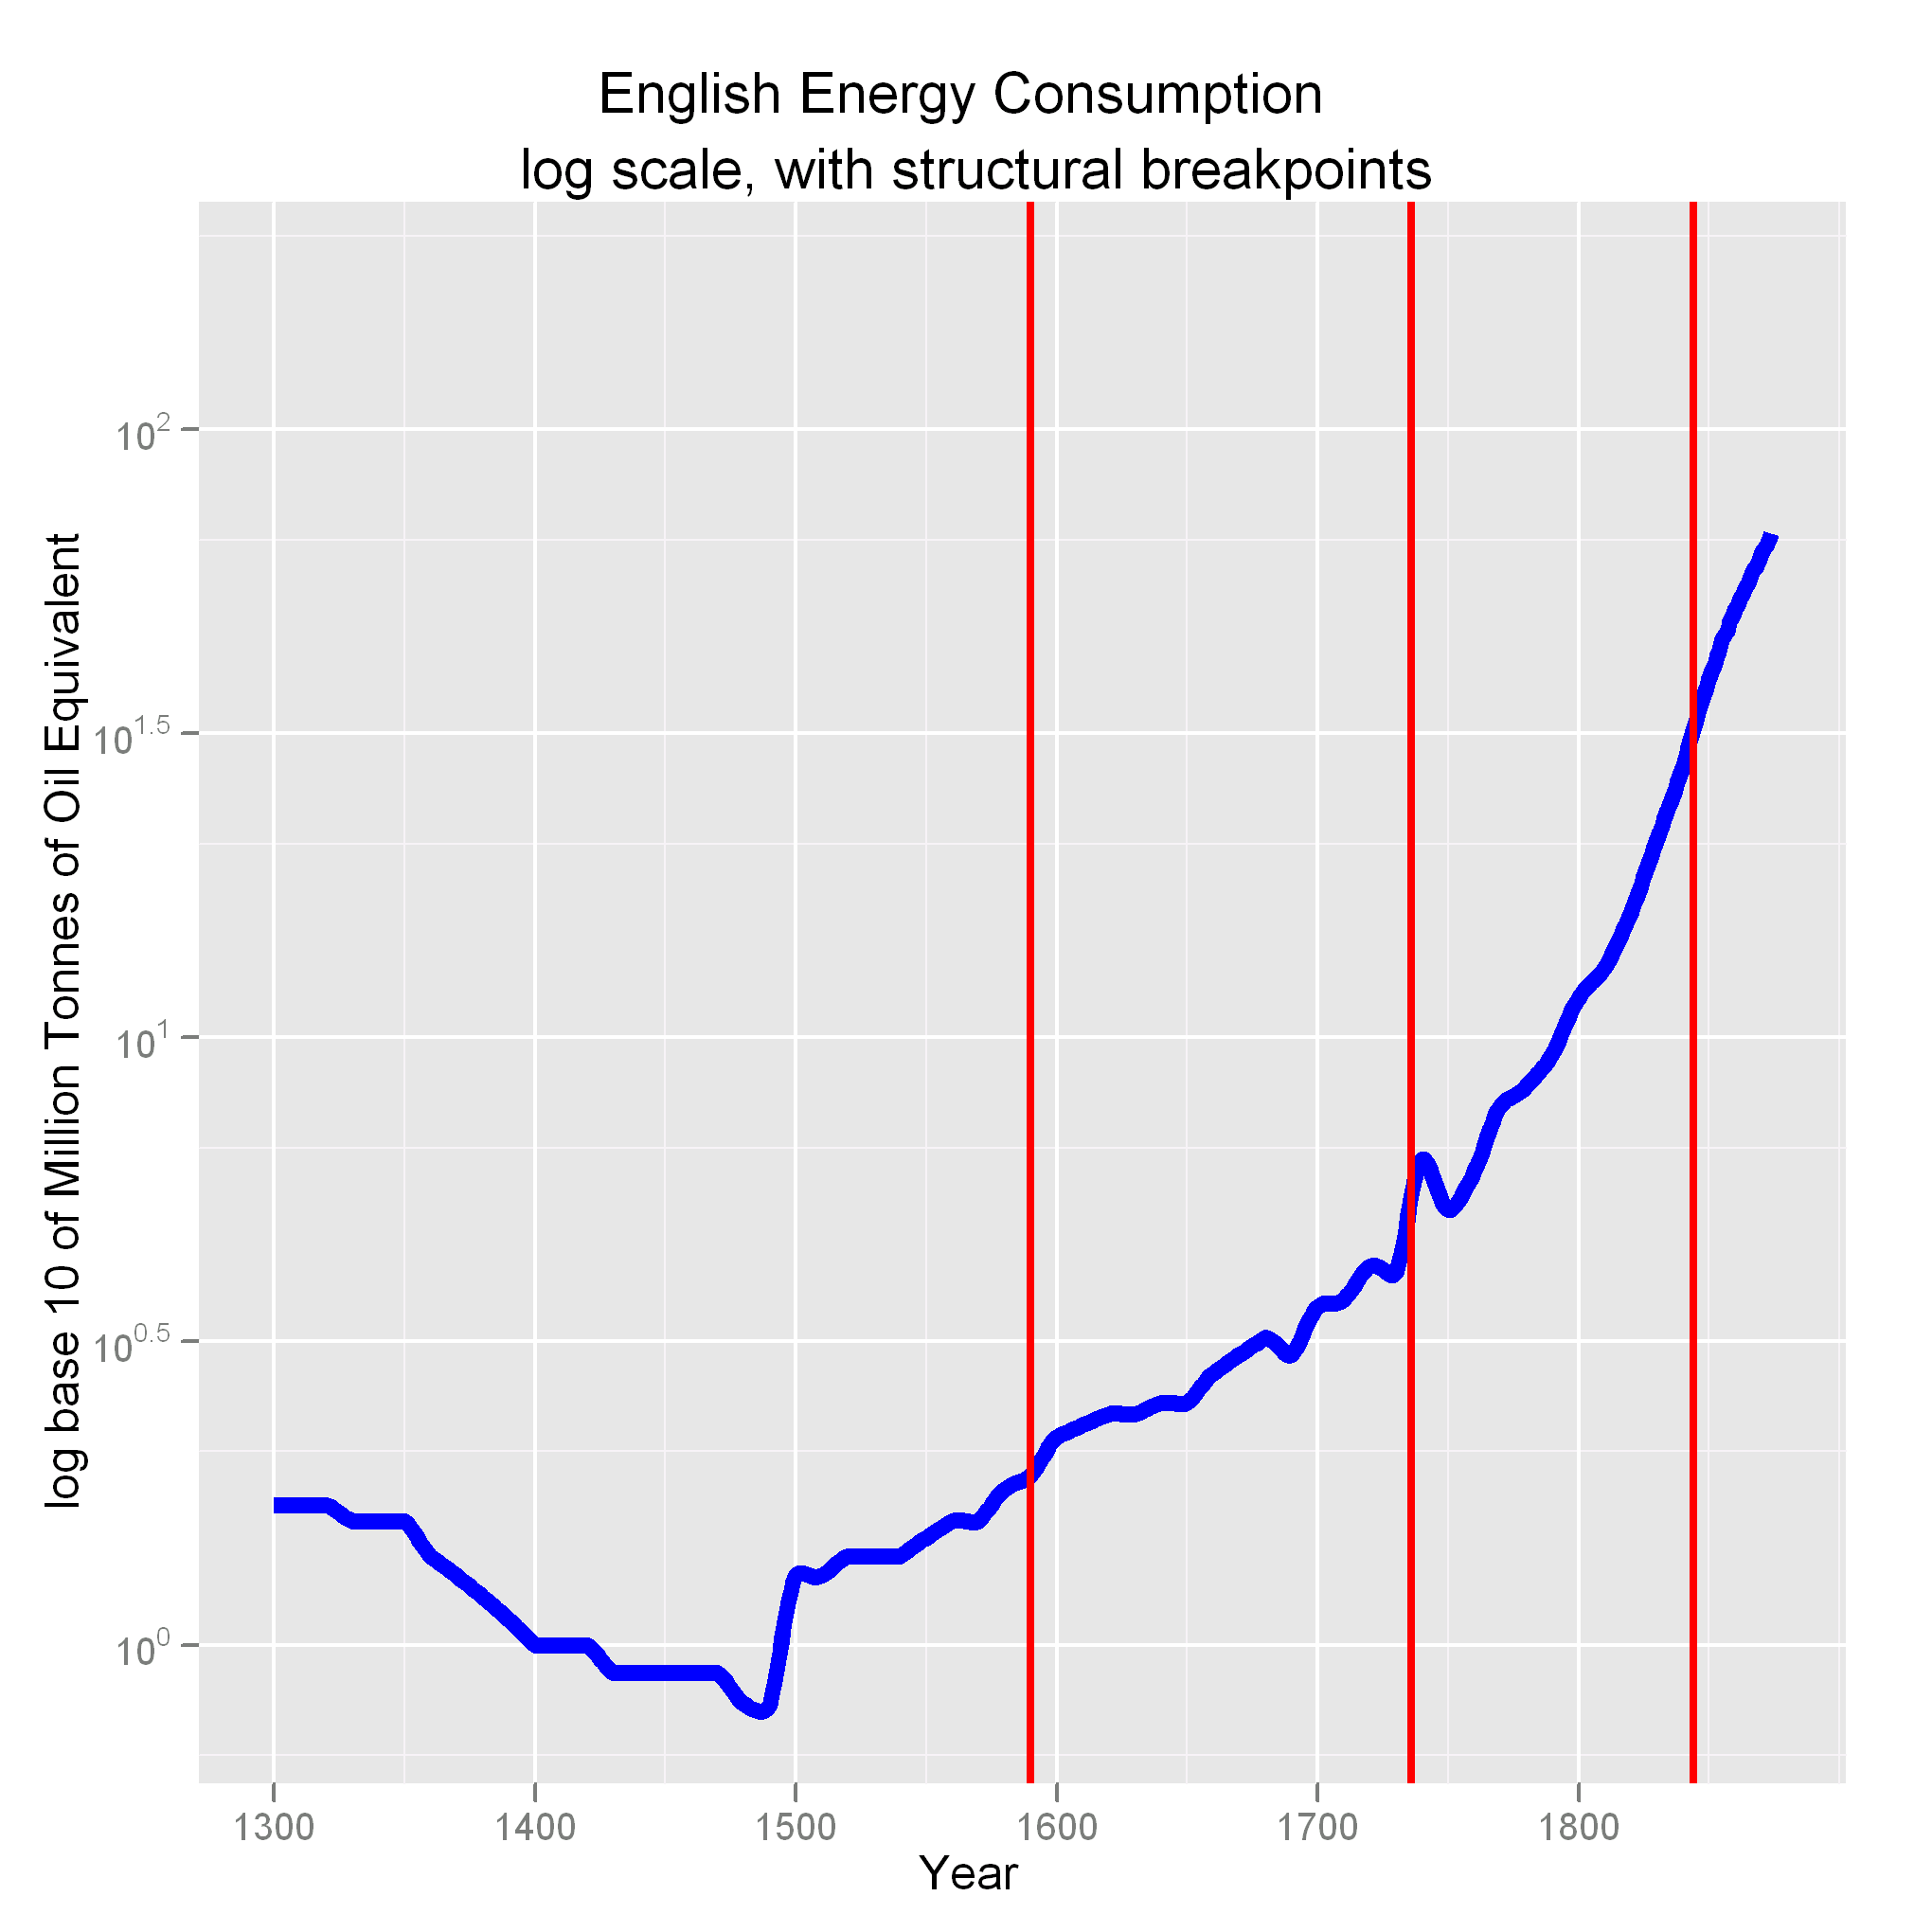
\includegraphics[width=0.33\textwidth]{../data/Analytics/notes/gbpmtoelog.png}
		\label{fig:subfig2}}
		\subfloat[diff \textit{log} energy consumption][Difference of \textit{log} of English energy consumption]{
		\includegraphics[width=0.33\textwidth]		{../data/Analytics/notes/gdifflogmtoe.png}
		\label{fig:subfig3}}
		
		\end{figure}
		

		\begin{figure}
%		\centering

		\caption[Levels, \textit{log} of levels and diffs of the time series]{Levels, \textit{log} of levels and first differences of logs of English GDP, with statistically significant breakpoints indicated by vertical lines on the log chart.}			\label{fig:globfig2}
				
		\subfloat[\textit{level} GDP][English GDP in levels]{
		\includegraphics[width=0.33\textwidth]{../data/Analytics/notes/ggdp.png}
		\label{fig:subfig4}}
		\subfloat[\textit{log} GDP][\textit{log} of English GDP]{
		\includegraphics[width=0.33\textwidth]{../data/Analytics/notes/gbpgdplog.png}
		\label{fig:subfig5}}
		\subfloat[diff \textit{log} energy consumption][Difference of \textit{log} of 				English energy consumption]{
		\includegraphics[width=0.33\textwidth] 	{../data/Analytics/notes/gdiffloggdp.png}
		\label{fig:subfig6}}
		
		\end{figure}

		\begin{figure}
		\centering

		\caption[Levels, \textit{log} of levels and diffs of the time series]{Levels, \textit{log} of levels and first differences of logs of the English population, with statistically significant breakpoints indicated by vertical lines on the log chart.}						\label{fig:globfig3}
		
		\subfloat[\textit{ln} population][\textit{ln} of English population in levels]{
		\includegraphics[width=0.33\textwidth]{../data/Analytics/notes/gpop.png}
		\label{fig:subfig7}}
		\subfloat[\textit{log} GDP][\textit{log} of English GDP]{
		\includegraphics[width=0.33\textwidth]{../data/Analytics/notes/gbppoplog.png}
		\label{fig:subfig8}}
		\subfloat[\textit{ln} diff population][\textit{ln} of first differences of English population]{
		\includegraphics[width=0.33\textwidth]{../data/Analytics/notes/gdifflogpop.png}
		\label{fig:subfig9}}
		
		\end{figure}		
		
%		\includepdfmerge[nup=2x3,noautoscale=true,scale=0.4,frame=true,offset=0 				-50,delta=0 10]						{../data/Analytics/notes/bpmtoe.png,../data/Analytics/notes/diffmtoe.png, ../data/Analytics/notes/bpgdp.png,../data/Analytics/notes/diffgdp.png, ../data/Analytics/notes/bppop.png,../data/Analytics/notes/diffpop.png}

%	\caption[
%	\textit{Ln} of levels and diffs of the time series]{\textit{Ln} of levels and first differences of the English time series, with statistically significant breakpoints indicated by vertical lines on the levels charts}


\newpage		
		\subsubsection{Stationarity}
		
		To further characterize the time-series, I tested each as a univariate \gls{arima} model using the $R$ \texttt{forecast} package \cite{hyndman_forecast:_2010}. The \texttt{auto.arima} method in \texttt{package::forecast} selects the appropriate model and allows incorporating exogenous (non-stochastic) inputs such as the time-series intervention variables described above.
		
		I note that after allowing for event interventions, both MTOE and GDP are $I(1)$ (non-stationary, or integrated of order one, mean a first difference or first derivative will be stationary. The population series is modeled as $I(0)$ (stationary), though the event interventions are not significant in this analysis. Each series analyzed without event dummies indicates $I(2)$, confirming the visual inspection results from figure \ref{fig:globfig1}.

		

		\begin{table}[h!]

		\begin{adjustwidth}{-0.75in}{}

		\caption[Summary \texttt{auto.arima} results]{This table contains the 		summary of the \texttt{auto.arima} analyses showing the results for no time intervention variables, and for results with time intervention variables}\label{tbl:station}

		\begin{tabular}{llrrrrrrrrr}
		\toprule \hline
		Breaks&Model&&Model&Variables&&&&&&\\
		\toprule \hline
		&MTOE&ar1&ar2&ar3&ar4&ma1&S1&S2&S3&drift\\
		\hline
		None&ARIMA(4,2,1)&0.8385& 0.5742&  -0.2776&  -0.3054&  -0.9334&&&\\
	    &s.e.        &0.0457&  0.0531&   0.0541&   0.0431&   0.0306&&&\\
		\hline
1590&ARIMA(4,1,1)&0.1880&1.3171&0.0014&-0.6435&0.8857&0.0065&0.0001&0.0004&-0.0049\\
1736&with drift&0.0354&0.0374&0.0341&0.0325&0.0270&0.0016&0.0016&0.0016&0.0019\\
1844&&&&&&&&&&\\
		\midrule \hline
		&GDP&ar1&ar2&ma1&ma2&ma3&ma4&S1&S2&S3\\
		\toprule
		None&ARIMA(1,2,4)&-0.6596&&0.3130&-0.6897&-0.1270&-0.1022&&&\\
	    &s.e.        &0.0608 &&0.0684&0.0492 &0.0613 &0.0531&&&\\
		\midrule
1556&ARIMA(2,1,3)&0.2427&0.7438&0.4158&-0.7589&-0.1777&&-0.0067&0.0030&-0.0156\\
1731&s.e.        &0.0467&0.0466&0.0634&0.0358&0.0600&&0.0030&0.0025&0.0062\\
1869&&&&&&&&&&\\
		\midrule \hline
		&Population&ar1&ar2&ma1&ma2&ma3&intercept&S1&S2&S3\\
		\toprule
		None&ARIMA(0,2,3)&&&-0.2994&-0.2525&-0.1521&&&&\\
	    &s.e.        &&&0.0410&0.0426&0.0411&&&&\\
		\midrule
1373&ARIMA(2,0,3)&1.9912&-0.9912&-0.2956&-0.2498&-0.1502&15.3036&-0.0016&-0.0017&-0.0017\\
1579&s.e.        &0.0072& 0.0072& 0.0416& 0.0429& 0.0415&    NaN& 0.0033&0.0033&0.0033\\
1774&&&&&&&&&&\\
		\bottomrule

		\end{tabular}
		\end{adjustwidth}
		\end{table}
		
		\newpage
		\subsubsection{Cointegration}
		
		Finally in this preliminary analytic exercise, I investigate the cointegration properties of the information set. To do so, I use the $R$ package \texttt{urca} as implemented from work done by Bernard Pfaff \cite{pfaff_analysis_2008}.
		
		The results are summarized in Table \ref{tbl:coint}. I model each series as a bivariate pair to assess the strength of any indicated cointegration relations and to support the multivariate modeling for the main analysis. I also model with different lag structures to assess robustness. The most robust bivariate result is between the MTOE and GDP pairs, with the second between the GDP and population pairs. These results support the multivariate modeling which indicates two cointegrating relations.
		
		The noteworthy result is that the cointegration relation between energy consumption and GDP is very strong, supporting my research hypothesis. These are preliminary, but encouraging, results. Further statistical testing awaits approval of this proposal.
		
		I also need to switch to the most robust cointegration software available, which is CATS in RATS as my analysis proceeds.
		

		\begin{table}[h!]
		\begin{center}
\caption[Johansen cointegration tests]{Johansen cointegration tests for English energy demand system; sample period 1300 - 1874 CE}\label{tbl:coint}
	
\begin{tabular} {llllrll}
\toprule \hline
&&No.&&&&\\
&Deterministic&of lagged&&Test& \multicolumn{2} {c} {Critical values} \\
\cmidrule (lr) {6-7}
Variables&terms&differences&$H_0:r=r_0$&statistic&$10\%$&$5\%$\\
\midrule
$e,g$&$tr,shift$&1&$r_0=0$&45.18&22.76&25.32\\
&&&$r_0=1$&0.81&10.49&12.25\\
&&&&&&\\
&&2&$r_0=0$&33.21&22.76&25.32\\
&&&$r_0=1$&0.79&10.49&12.25\\
&&&&&&\\
$e,p$&$tr,shift$&1&$r_0=0$&41.49&22.76&25.32\\
&&&$r_0=1$&12.45&10.49&12.25\\
&&&&&&\\
&&2&$r_0=0$&33.51&22.76&25.32\\
&&&$r_0=1$&10.20&10.49&12.25\\
&&&&&&\\
$g,p$&$tr,shift$&1&$r_0=0$&43.29&22.76&25.32\\
&&&$r_0=1$&6.02&10.49&12.25\\
&&&&&&\\
&&2&$r_0=0$&35.73&22.76&25.32\\
&&&$r_0=1$&5.97&10.49&12.25\\
&&&&&&\\
$e,g,p$&$tr,shift$&1&$r_0=0$&78.54&39.06&42.44\\
&&&$r_0=1$&41.45&22.76&25.32\\
&&&$r_0=2$&5.16&10.49&12.25\\
&&&&&&\\
&&2&$r_0=0$&63.06&39.06&42.44\\
&&&$r_0=1$&28.94&22.76&25.32\\
&&&$r_0=2$&5.42&10.49&12.25\\
\bottomrule
\end{tabular}

\caption*{\textit{Notes:} \textit{e}-ln of MTOE (million tonnes of oil equivalent), \textit{g}-ln of GDP, \textit{p}-ln of population. For the model's deterministic components: \textit{c}-constant, \textit{tr}-linear trend, \textit{shift}-shift dummy $dsubS3$; critical values from Johansen.}
\end{center}
\end{table}

		\newpage


	\section{Completion Timetable}
		\begin{tabular}{ll}
		Event&Date\\
		\midrule
		Draft Proposal&August 2011\\
		Topic Defence&Spring 2012\\
		Draft Dissertation&Fall 2012\\
		Final Defence&Fall 2012\\
		\bottomrule
		\end{tabular}
	
	
	\section{Annotated Bibliography}
		\bibliography{scbdissertation}
%		\bibliography{exporteditems}
	
	\section{Glossary}
	\printglossaries
	
\begin{comment}
$12^{th}$ century renaissance \url{http://en.wikipedia.org/wiki/Renaissance_of_the_12th_century}
\end{comment}

\appendix
\section{Detailed Statistical Methodology} 
\label{sec:Appendix A}

	Note that these step-by-step details are mainly notes to myself regarding the Copenhagen methodology at a detailed level. I include them here for interested readers, but the proposal should be understandable without this detail for most.

			\begin{enumerate}

				\item Description of the logic of the methodology (the probability approach in VAR econometrics):
				
				 ``The vector autoregressive (VAR) process based on Gaussian (normally distributed) errors has frequently been a popular choice as a description of macroeconomic time-series data.
				
			Theory-based economic models have traditionally been developed as non-stochastic mathematical entities and often applied to empirical data by adding a stochastic error process to the mathematical model.
			
			From an econometric point of view, the two approaches are fundamentally different: one starting  from an explicit stochastic formulation of \textit{all} data and then \textit{reducing} the general statistical (dynamic) model by imposing testable restrictions on the parameters, the other starting from a mathematical (static) formulation of a theoretical model and then \textit{expanding} the model by adding stochastic components.''
			\footnote{Juselius 2006 chapters 1--3} %%Juselius 2006 ch1-3

				\item Investigate the unrestricted VAR
				\begin{enumerate}
					\item Estimate the unrestricted VAR for the information set
					\item Select and form the \gls{ecm} representation
					\item Perform misspecification tests
					\begin{enumerate}
						\item Perform specification checking
						\item Test residual correlations and use information criteria to identify lag lengths
						\item Test residual autocorrelation 
						\item Test residual heteroskedasticity
						\item Perform normality tests
					\end{enumerate}
				\end{enumerate}
				\item Investigate deterministic components in the model. \footnote{Juselius 2006 chapter 6} %% Juselius ch6
				\begin{enumerate}
					\item Identify possible deterministic cases. The reference model is the simple $VAR(1)$ containing a constant, $\boldsymbol{\mu}_0$, and a trend, $\boldsymbol{\mu}_1t$ in $AR$ form:
					\begin{equation}
					\Delta \bold{x}_t = \boldsymbol{\alpha \beta}'\bold{x}_{t-1} + \boldsymbol{\mu}_0 + \boldsymbol{\mu}_1t + \boldsymbol{\epsilon}
					\end{equation}
					\begin{enumerate}
						\item Case 1. $\boldsymbol{\mu}_1$, $\boldsymbol{\mu}_0 = \bold{0}$. This case corresponds to a model with no deterministic components in the data, i.e. $E(\bold{\Delta} \bold{x}_t)=\bold{0}$ and $E(\boldsymbol{\beta}^{'} \bold{x}_t) = \bold{0}$
						\item Case 2. $\boldsymbol{\mu}_1=\bold{0}$, $\boldsymbol{\gamma}_0=\bold{0}$ but $\boldsymbol{\beta}_0 \neq \bold{0}$, where $\boldsymbol{\gamma}_0$ is defined as a term in the decomposition of $\boldsymbol{\mu}_0=\boldsymbol{\alpha \beta}_0 + \boldsymbol{\gamma}_0$.
						\item Case 3. $\boldsymbol{\mu}_1= \bold{0}$, i.e. $(\boldsymbol{\beta}_1, \boldsymbol{\gamma}_1)= \bold{0}$, and the constant term $\boldsymbol{\mu}_0$ is \textit{unrestricted}, i.e. no linear trends in the $VAR$ model, but linear trends in the variables, where $\boldsymbol{\gamma}_1$ is defined as a term in the decomposition of $\boldsymbol{\mu}_1=\boldsymbol{\alpha \beta}_1 + \boldsymbol{\gamma}_1$.
						\item Case 4. $\boldsymbol{\gamma}_1 = \bold{0}$, but $(\boldsymbol{\gamma}_0,\boldsymbol{\beta}_0,\boldsymbol{\beta}_1) \neq \bold{0}$, i.e. the trend is \textit{restricted} only to appear in the conintegrating relations, but the constant is unrestricted in the model.
						\item Case 5. No restrictions on $\boldsymbol{\mu}_0, \boldsymbol{\mu}_1$, i.e. trend and constant are \textit{unrestricted} in the model.
					\end{enumerate}
					\item In $MA$ common trends form to clarify the source of linear trends:
					\begin{equation}
					\bold{x}_t = \boldsymbol{\beta}_\bot(\boldsymbol{\alpha}_\bot ' \boldsymbol{\Gamma} \boldsymbol{\beta}_\bot)^{-1} \boldsymbol{\alpha}_\bot '\left\lbrace \boldsymbol{\gamma}_0 t + \frac{1}{2} \boldsymbol{\gamma}_1 t + \frac{1}{2} \boldsymbol{\gamma}_1 t^2 \right\rbrace + \bold{C}^*(L) \boldsymbol{\mu}_1 t
					 + \bold{C}^*(1) \boldsymbol{\mu}_0 + \bold(C) \displaystyle\sum\limits_{i=1}^t \boldsymbol{\epsilon}_t + \bold{C}^*(L) \boldsymbol{\epsilon}_t + \bold{\tilde{X}}_0
					\end{equation}
					Thus, the linear trends in the variables can originate from three different sources in the $VAR$ model:
					\begin{enumerate}
						\item[1.] the $\boldsymbol{\alpha}$ component $(\bold{C}^*(L) \boldsymbol{\mu}_1 t)$ of the unrestricted linear trend $\boldsymbol{\mu}_1 t$;
						\item[2.] the $\boldsymbol{\beta}_\bot$ component $(\boldsymbol{\gamma}_1 t)$ of the unrestricted linear trend $\boldsymbol{\mu}_1 t$;
						\item[3.] the $\boldsymbol{\beta}_\bot$ component $(\boldsymbol{\gamma}_0 t)$ of the unrestricted constant term $\boldsymbol{\mu}_0$.
					\end{enumerate}
					\item Consider intervention \textit{(dummy)} variables. Similarly as for the trend and constant, consider a simple regression model for $x_t$ containing three different types of dummy variables:
					\begin{equation}
					x_t = \phi_s D_{s,t} + \phi_p D_{p,t} + \phi_{tr} D_{tr,t} + u_t + x_0
					\end{equation}
					where $D_{s,t}$ is a mean-shift dummy $(\dots,0,0,0,1,1,1,\dots)$, $D_{p,t}$ is a permanent intervention dummy $(\dots,0,0,1,0,0,\dots)$, and $D_{tr,t}$ is a transitory shock dummy $(\dots,0,0,1,-1,0,0.\dots)$ and the residual is a first order autoregressive process with form:
					\begin{equation}
					u_t = \frac{\epsilon_t}{1-\rho L}
					\end{equation}
					Which for difference non-stationary series results in a change of form as follows:
					\begin{equation}
					\Delta x_t = \phi_s \Delta D_{p,t} + \phi_p \Delta_{tr,t} + \phi_{tr} \Delta_{dtr,t} +  \epsilon_t,
					\end{equation}
					i.e. a shift in the levels of a variable becomes a `blip' in the difference variable, a permanent `blip' in the levels becomes a transitory blip in the differences, and a transitory blip in the levels becomes a double transitory blip, $D_{dtr,t}$, in the differences.
					
					My plan is to analyse the time series for structural breaks, formulate dummy variable(s) appropriately, then test whether the dummies are significant, and for which equations in the $VAR$.
				\end{enumerate}
				\item Estimate the $I(1)$ model. \footnote{Juselius 2006 chapter 7} %%Juselius ch7
				\begin{enumerate}
					\item Preliminary estimates of the English data indicate that the series, \textit{with time dummies included}, are integrated of order one $I(1)$.  This, of course, is essential in determining the formally correct methodology as $I(2)$ forms require a modified technique.  However, practical considerations, for example lack of $I(2)$ support in current software, dictate that I will use $I(1)$ methodology, BUT will check for signalling of $I(2)$ problems.
					\item Concentrating the general $VAR$ model.
					
					Proceeding under the $I(1)$ assumption, and under the assumption that the empirical $VAR$ can describe the data, we can state the $I(1)$ condition as:
					\begin{equation}
					\boldsymbol{\Pi} = \boldsymbol{\alpha \beta'},
					\end{equation}
					where $\boldsymbol{\alpha}$ and $\boldsymbol{\beta}$ are $p \times r$ matrices.  If $r = p$, then $\bold{x}_t$ is stationary and classical inference applies.  If $r = 0$, then there are $p$ autonomous trends in $\bold{x}_t$ so that each $x_{i,t}$ is non-stationary with its own individual trend.  In this case the vector process is driven by $p$ different stochastic trends and it is not possible to obtain stationary cointegration relations between the levels of the variables.  Also, the variables have no stochastic trends in common and, hence, do not move together over time.
					
					Should this be the case, I will reformulate the $VAR$ model in levels as a $VAR$ model in differences \textit{without any consequential loss of long-run information} and classical inference applies.
					
					If $p > r > 0$, then $\bold{x}_t \sim I(1)$ and there exist $r$ directions into which the process can be made stationary by linear combinations.  These are the cointegrating relations, which often can be interpreted as deviations from economic steady-state relations, and are thus economically meaningful.
					\item Derive the maximum likelihood (ML) estimator of the concentrated model.
					
					Assuming a finding of cointegrating relations, I proceed to use ML to estimate the long-run equilibrium relations from a concentrated model of the form (disregarding for the moment deterministic elements):
					\begin{equation}
						\bold{R}_{0t} = \boldsymbol{\alpha \beta'}\bold{R}_{1t} + \boldsymbol{\epsilon}_t, \quad \boldsymbol{\epsilon}_t \sim N_p(\bold{0},\boldsymbol{\Omega}).
					\end{equation} Note that at this point the estimating task has been separated into long-run and short-run processes, an essential part of the methodology, and allowed under the Frisch-Waugh theorem.
					\item Normalize the results.
					
					This step allows an economic interpretation of a cointegrating relation, and thus one should choose a meaningful normalizing variable. Note, however, that the cointegrating relations are not sensitive to the choice of normalizing variable. Note that this is the so-called ``Johansen" procedure.
					\item Interpret the unrestricted results.
					
					While the unrestricted $\boldsymbol{\hat{\alpha}, \,\hat{\beta}, \text{ and } \hat{\Pi}}$ are not expected to yield directly interpretable results, they may, so I will proceed by inspecting them.
				\end{enumerate}
				\item Determine the cointegration rank. \footnote{Juselius 2006 chapter 8}  %%Juselius ch 8
				
				This is an essential step as it influences subsequent inference and economic interpretation. The actual test statistics are likelihood ratios (LR), and are compared to carefully specified asymptotic distributions to yield critical values.
				
				The cointegrating rank divides the data into $r$ relations towards which the process is adjusting, and $p - r$ relations which are pushing the process. The former are interpreted as (initially) statistical equilibrium errors (deviations from a statistical steady-state), and the latter as common driving trends in the system.
				\item Cointegration hypotheses testing--recursive tests of parameter constancy. \footnote{Juselius 2006 chapter 9}
				
				In this step I will perform four classes of tests for parameter constancy, using both statistical and graphical methods.
				\begin{enumerate}
					\item Recursive tests of the full model, essentially a recursive test of the likelihood function, which will indicate whether the model is approximately acceptable.  This is conceptually similar to recursive Chow tests for single-equation models.
					\item Recursive tests on the eigenvalues, $\lambda_i$ and transformations of them, which will provide more detailed constancy information about individual cointegrating relations.
					\item Recursive tests of the constancy of the cointegration space, $\boldsymbol{\beta' x_t}$.
					\item Recursive tests of predictive failure for both the full system and individual series.
					\item Judging the effects of any found parameter instability.
				\end{enumerate}
				\item Cointegration hypotheses testing--testing restrictions on $\boldsymbol{\beta}$. \footnote{Juselius 2006 chapter 10}
				
				This process will help in spotting potentially relevant long-run relations, and requires several steps:
				\begin{enumerate}
					\item Formulate hypotheses as restrictions on $\boldsymbol{\beta}$.
					\item Testing the same restriction on all cointegration relations.
					\item Testing the stationarity of a known $\boldsymbol{\beta}$ vector.
					\item Testing the stationarity of a cointegration relation when some coefficients are know and others must be estimated.
				\end{enumerate}
				\item Cointegration hypotheses testing--testing restrictions on $\boldsymbol{\alpha}$. \footnote{Juselius 2006 chapter 11}
				
				Tests on $\boldsymbol{\alpha}$ are closely associated with interesting hypotheses about the common driving forces in the system.  
				
				The test of zero row in $\boldsymbol{\alpha}$ is the equivalent of testing whether a variable can be considered weakly exogenous for the long-run parameters $\boldsymbol{\beta}$.  These define a common driving trend as cumulative sums of empirical shocks to variables.
				
				The test of a unit vector in $\boldsymbol{\alpha}$ defines a variable which is exclusively adjusting, and whose shocks have no permanent effect on any of the variables in the system.
				
				Thus, the two types of test can identify the pushing and pulling forces of the system.
				\begin{enumerate}
					\item Testing for long-run weak exogeneity.
					\item Testing for weak exogeneity in partial models.
					\item Testing a known vector in $\boldsymbol{\alpha}$.
					\item Interpret the results on $\boldsymbol{\beta}$ and $\boldsymbol{\alpha}$ in terms of economic scenarios.
				\end{enumerate}
				\item Identification--identify the long-run structure. \footnote{Juselius 2006 chapter 12} %%Juselius 2006  ch 12
				\begin{enumerate}
					\item Formulate identifying hypotheses and degrees of freedom
					\item Consider just-identifying restrictions
					\item Consider over-identifying restrictions
					\item Consider lack of identification
					\item Perform recursive diagnostic tests of $\alpha$ and $\beta$
				\end{enumerate}
				\item Identification--identify the short-run structure. \footnote{Juselius 2006 chapter 13}	%% Juselius 2006 ch 13
				\begin{enumerate}
					\item Formulate identifying restrictions
					\item Interpret shocks
					\item Formulate the short-run economic questions
					\item Consider restrictions on the short-run reduced-form model
					\item Construct \textit{VAR} in triangular form
					\item Formulate empirically identifiable current effects
					\item Construct the preferred structure
				\end{enumerate}
				\item Identification--identify common trends. \footnote{Juselius 2006 chapter 14} %%Juselius 2006 ch 14
				\begin{enumerate}
					\item Formulate the common trends representation
					\item Formulate the unrestricted MA representation
					\item Formulate the MA representation subject to restrictions on $\alpha$ and $\beta$
					\item Impose exclusion restrictions on $\beta_\bot$
					\item Assess the economic model scenario
				\end{enumerate}
				\item Identification--identify a structural MA model. \footnote{Juselius 2006 chapter 15} %% Juselius ch 15
				\begin{enumerate}
					\item Reparameterize the VAR model
					\item Separate between transitory and permanent shocks
					\item Formulate and interpret structural shocks
					\item Test the credibility of the labels on the economic shocks
				\end{enumerate}
			\end{enumerate}
			
\section{Table of variable, coefficient, and function definitions} 
\label{sec:Appendix B}
\centering
%\begin{center}
\begin{longtable}{ll}
\toprule
Variable&Description\\
\toprule
$\bold{x}_i , i=0 \cdots k-1$&m x 1 vector of endogenous variables\\
$m$&number of endogenous variables\\
$k$&number of lags for independent endogenous variables\\
$\Delta \bold{x}_i$&first difference of endogenous variables\\
$\boldsymbol{\mu}_0$&m x 1 vector of intercept coefficients\\
$\boldsymbol{\mu}_1$&m x 1 vector of time-dependent coefficients\\
$t$&sequentially enumerated time period\\
$AR$&auto-regressive specification\\
$E$&probabilistic expectations operator\\
$\boldsymbol{\Pi}(=\boldsymbol{\alpha}\boldsymbol{\beta}')$&m x m matrix of dynamic coefficients relating $\Delta \bold{x}_t$ to past values of $\bold{x}_t$\\
$\boldsymbol{\alpha}$&m x r matrix of adjustment coefficients describing how equilibrium deviations feed back onto $\bold{x}_t$\\
$\boldsymbol{\beta}'$&r x m matrix of deviations from equilibrium\\
$r$&number of cointegrating relationships\\
$\boldsymbol{\gamma}$&a term which allows us to decompose $\boldsymbol{\alpha\beta}'$ into further usable terms\\
$MA$&moving average common trends specification\\
$\boldsymbol{\beta}_\bot$&orthogonal complement of $\boldsymbol{\beta}'$\\
$\boldsymbol{\alpha}'_\bot$&orthogonal complement of $\boldsymbol{\alpha}$\\
$\boldsymbol{\Gamma}$&m x m matrix of coefficients relating $\Delta \bold{x}_t$ to past values of $\Delta \bold{x}_{t-i}$\\
$\bold{C}$&m x m matrix of coefficients in moving average representation of VAR to evaluate deterministic trends in cointegrating relationships\\
$L$&lag operator representing the number of past periods of endogenous variable data to be included\\
$\bold{R}$&concentrated notation of VAR model for notational simplicity\\


\end{longtable}
%\end{center}

\end{document} \section{End}

\section{notes}
\subsection{2013 EHA notes}
Nef, Habakuk\\
Agriculture transition\\

\subsection{Thirsk 05/13}
ISI, government encouraged, sponsored\\
demand?\\

\subsection{committee notes}
Tim -- remove personal references e.g. Marx  %done 10/13/11
Tim -- quantitative measure of unlimited energy % so lewis talked about labour with at zero marginal product. my idea is that, relative to any labor supply, the amount of mineral energy was essentially unlimited for the initial developing economies. another way of thinking of it is the human energy chart. an interesting question is whether pure energy has diminish marginal product, I think not, thus that you have to look at specific sources and their physical requirements to determine the amount of diminishing marginal product, and in any case it is less than human labour.  10/13/11. %done 11/14/11.

Richard -- other metric approaches. %Why, since looking at graphs of gdp and energy consumption per capita presents such a clear relationship, do I consider a more detailed statistical look? I am interested in looking inside the dynamics that are supported by the long period time series. What this examination should tell is whether the the prime dynamic drivers, so the leading-in-time variables, changed places in the short run and the long run in the economies I study. While I purposefully avoid the term causality at this point, depending on the strength of the results, I may find causality in the data. What I want to understand, beyond my hypothesis of centrality of mineral energy consumption as the defining invention of the Industrial Revolution, is what implications this has for modern development and for sustained per capita economic development in an age of potentially emission constrained economies. The time series methodology I propose has the ability to do this. And it has the capability of incorporating important time related events that enter the time series as discontinuties. Both of these capabilities are core to my research. 10/14/11. %done 11/14/11.

11/17
Rudi - 5 major items. mainly tighten. He thinks if I do a 2-3 page abstract of intro section, Lance might be interested.

You've done already a lot of work. On a lot of this I am no expert (neither history nor metrics). So bear with me.
Let me jot down just a few quick notes:


\begin{itemize}
\item 1) Presentation: Put hypothesis first; don't make the reader wait or search. In this draft, and in a later paper, and in your presentation, the juxtaposition of the various explanations should come much earlier. I.e.: On the first page (!!), there should be a paragraph saying that "the industrial revolution in England is commonly explained by (1) cultural exceptionalism, wihch essentially means ... , (2) ... , (3) energy, .... (4) thermodynamics. My hypothesis is that (x) matters more than previously believed, and my dissertation tests the evidence for that. The anecdotal evidence includes the lack of Dutch industrialization ... etc. " 

\item 2) Hypothesis: Sharpen it. How distinct is your hypothesis really from culture/institution-driven explanations? You do argue that all, even cultural exceptionalists, place emphasis on coal. It might be reasonable to say that the explanation must be found in a combination of these factors -- and your contribution is to "shift the weights." Is that about right? It could be fleshed out more, sharpened at the edges.

\item 3) Metrics: Institutional variables. I didn't go through the details. Do you use some proxies for institutional development, or cultural factors? Should that be there, if you want to compare the influence of those variables to energy? 

\item 4) Contributions: Limit yourself. Section 2.1.2 is too broad, and contains too much, I would say. It is not clear what you mean by 5., and, if clarified, it is by itself possibly a whole dissertation. I would drop it for now. 3. and 4. should go together. Arguably, 4. might be post-dissertation research. You want a classic 3 goals (and papers) in here: (1) Literature review, which you've done in part;  (2) Explanation and re-evaluation of the industrial revolution in England in the language of economic history; (3) Explanation and re-evaluation of the industrial revolution in England in the language of econometrics. 

\item 5) The link to growth theory: Rather than 5., you might want to consider "old" growth theories. You make reference to Lewis. So combine Lewis (or Marx and Kalecki, really) with Malthus, and see where that takes you. Lewis warns of the turning point, when surplus labor is exhausted, and real wages must rise. If energy is the real labor, then we might be there. What does that mean for future growth? That's an interesting question, and you can fruitfully feed future research --- but I would try to make these three papers quite focused on what you have in mind now. 

\end{itemize}


thinks I could do england vs holland and nail that. would need dutch energy series.

Tim - wants me to change graphs, support his method, has many notes, likes my lit review.

\begin{itemize}
\item 
\end{itemize}

\begin{itemize}
\item Why time series
\item Various ts approaches
\item univariate arima
\item static
\item ardl
\item var
\item cointegrated var

\end{itemize}

may use the Diebold 98 article for organizing, or Dougherty

\subsection{sequence for bibliography}

pdflatex
bibtex on .bib F11
pdflatex
pdflatex
bibtex on .tex  F11
pdflatex
pdflatex

sequence for glossary

    Build LaTeX document, this will generate the files used by makeglossaries
    Run the indexing/sorting, the recommended way is to use makeglossaries (a script that runs xindy or makeindex depending on options in the document with correct encoding and language settings):

    makeglossaries <myDocument>

    Build LaTeX document again to get document with glossary entries


\begin{comment}
% save just for reference...covered by table and annotated bib
		\subsection{Data Sources}
		I anticipate using a wide variety of sources. Should I just do a bibliography here?
			\subsubsection{English historical-institutional sources}
			\begin{itemize}
			\item Wrigley
			\item van Zanden
			\item for reference, list in Wrigley discussion
			\item Landes
			\item Crafts
			\item Temin
			\item Pomeranz
			\item Allen
			\item Mokyr
			\item Goldstone
			\item McCloskey
			\item de Vries
			\item Jevons
			\item Clark
			\item TS Ashton
			\end{itemize}
			\subsubsection{English long-period time series sources}
			\begin{itemize}
			\item Mitchell
			\item Snooks
			\item Officer
			\item Fouquet
			\item Warde
			\item Maddison
			\end{itemize}
			\subsubsection{U.S. historical-institutional sources}
			\begin{itemize}
			\item Vaclav Smil
			\item Daly and Townsend
			\item Lewis
			\item North
			\end{itemize}
			\subsubsection{U.S. long-period time series sources}
			\begin{itemize}
			\item Historical Statistics of the United States 1780-1945
			\item Historical Statistics of the United States Millennial Edition Online
			\item Historical, Demographic, Economic, and Social Data: The United States, 1790-2002
			\item Gordon Whitney
			\item Kindleberger
			\end{itemize}
			\subsubsection{Chinese historical-institutional sources}
			\begin{itemize}
			\item Xu, Dixin, and Zhengming Wu, eds. 2000. Chinese Capitalism, 1522-1840. New York: St. Martin's Press.
			\item Hsien-Chun Wang. 2009. ``Discovering Steam Power in China, 1840s-1860s." Technology and Culture 51(1): 31-54.
			\item ``Pomeranz, K.: The Great Divergence: China, Europe, and the Making of the Modern World Economy."
			\item Andre Gunder Frank
			\item Janet Abu-Lughod
			\item Jack Goldstone
			\end{itemize}
			\subsubsection{Chinese long-period time series sources}(May not be available)
			\begin{itemize}
			\item Sinton, Jonathan E. 2001. ``Accuracy and reliability of China's energy statistics." China Economic Review 12(4): 373-383.
			\item Chinese Statistical Yearbook
			\end{itemize}
			\subsubsection{World long-period time series sources}
			\begin{itemize}
			\item Payne - a literature review of recent energy-gdp empirical studies
			\item US DOE EIA
			\item OECD
			\item UN
			\item Katarina Juselius. 2010. On the Role of Theory and Evidence in Macroeconomics. University of Copenhagen. Department of Economics.
			\item Epic of Gilgamesh. The tablets VII and  XI story of the flood. BC 2700. As a hook on which to illustrate the length of time between the Neolithic and Industrial revolutions. One of very earliest histories. So we know about half the 10K years, and there is essentially nothing economically that happened.
			\item Michael Kremer, 1993. Population Growth and Technological Change: One Million B.C. to 1990.
			\item Johansen et al. 2000 Cointegration analysis in the presence of structural breaks
			\item Foley 1996 Statistical Equilibrium Models in Economics
			\end{itemize}
\end{comment}			

\begin{comment}
%leave this out as the glossary is linked		
		\subsection{Definition of Terms}
		\begin{itemize}
		\item \gls{organic}
		\item \gls{mineral}
		\item \gls{neorev}
		\item \gls{insolation}
		\item \gls{areal}
		\item \gls{punctiform}
		\item \gls{indrev}
		\item \gls{early}
		\item \gls{high}
		\item \gls{earmodern}
		\item \gls{modern}
		\item \gls{energy}
		\item \gls{growth}
		\end{itemize}
\end{comment}		

in the full writeup, I need to highlight the ironic effloressence description of jack goldstone.

data sources -- maddison chinese stats 1998 oecd

data sources -- mitchell on american stats

\subsection{Methodology notes}

Cleaning time series data\\
http://www.r-bloggers.com/cleaning-time-series-and-other-data-streams/
\\
package::pracma, method::outlierMAD. Instances of 'moving window data cleaning'\\
\fi
\iffalse
\documentclass[11pt]{article}
\title{Energy and institutions: What \textit{really} happened in the English Industrial Revolution? What did not happen in China?}
\author{Stephen C. Bannister\\
	Department of Economics\\
	University of Utah\\
	Salt Lake City, Utah 84112\\
	USA\\
	\href{mailto:steve.bannister@econ.utah.edu}{steve.bannister@econ.utah.edu}\\
	}

%\date{Drafts May 2012,}
\date{}

\usepackage[latin1]{inputenc}
%\usepackage[english]{babel}
\usepackage{amsmath}
\usepackage{amsfonts}
\usepackage{txfonts}
\usepackage{amssymb}
\usepackage{pgfpages}
\usepackage{booktabs}
\usepackage{longtable}

\usepackage{chngpage}
%\usepackage{pdfpages}
\usepackage{graphicx}
\usepackage[lofdepth,lotdepth,position=bottom]{subfig}
\usepackage{caption}
\usepackage{float}
%\usepackage{draftwatermark}

%\newtheorem{mydef}{Definition}[section]
%\numberwithin{equation}{section}


\usepackage{verbatim}
%\usepackage{underscore}
\linespread{1.9}	% remove for single, 1.3 for 1.5 and 1.6 for 2.0. use this setting for print editing

\usepackage{glossaries}

\graphicspath{{C:/Users/Steve/Documents/GitHub/publish/diss1/images/}}

%\textwidth{7.5in}
\addtolength{\textwidth}{1.0in} 
\addtolength{\oddsidemargin}{-0.5in} 
\addtolength{\evensidemargin}{-0.5in} 
\addtolength{\textheight}{1.25in}
\addtolength{\topmargin}{-0.75in}

\usepackage{tocloft}

\usepackage{natbib}
\bibpunct{(}{)}{;}{a}{,}{,}

\usepackage{hyperref}


\makeglossaries

%\loadglsentries{glossary.tex}

%\setcounter{secnumdepth}{4}%to number paragraphs so can ref them?

\begin{document}

%\SetWatermarkLightness{0.93}
%\SetWatermarkScale{1}

	\maketitle
%	\nocite{*}
%	\bibliographystyle{E:/LaTeX-Portable/MikTex-Portable/bibtex/bst/base/IEEEanot}

%	\bibliographystyle{E:/LaTeX-Portable/MikTex-Portable/bibtex/bst/base/plain-annote}
%	\bibliographystyle{plain}


%\newcommand{\listequationsname}{List of Equations}
%\newlistof{myequations}{equ}{\listequationsname}
%\newlistof{myequations}{equ}{\listequationsname}
%\newcommand{\myequations}[1]{%
\addcontentsline{equ}{myequations}{\protect\numberline{\theequation}#1}\par}
\fi

\chapter{Energy and institutions: What \textit{really} happened in the English Industrial Revolution? What did not happen in China?}

\section{Introduction}
%\begin{abstract}
	
	England during the period leading up to and spanning the first Industrial Revolution collectively learned how to consume a virtually unconstrained quantity of fossil (mainly coal) energy. Led by the period's effective aggregate demand growth this resulted directly in productivity growth that then led to modern economic growth in living standards for the first time in recorded history. 
		
	Studying the event empirically we can use recent long--period series estimates of levels of English energy consumption, gross domestic product, and population to test the hypothesis that this was primarily an \textit{energy} revolution with important but mostly proximate institutional and cultural support.
	
	Then a natural experiment is run using Ming and Qing China using limited data and important institutional comparisons that would not preclude China from completing an industrial revolution. In order to explain the English success and the Chinese failure a theoretical framework for industrial revolutions is explored.
	
	The outcome should provide insights into economic development for growth economists by highlighting the importance of energy transitions for growth of economic systems. Additionally, the analytic framework developed can be applied across time and geography adding insights to ongoing development puzzles.% and to the realistic chances of curbing ecologically damaging mineral (fossil) energy consumption for ecological economists and others interested in that critical topic.
%	\end{abstract}



\subsection{English energy data}

	As early as 1734 observers of the economic panorama, later including economic and other historians, have commented on the role of energy inputs in economic activity and its social outcomes. These comments are not always explicitly related to energy but their implications often are. Jean Theophilus Desaguliers \cite{desaguliers_course_1734} was a member of the Royal Society and ``natural philosopher'' (physicist and engineer) and observes that using human labor to pump water from coal mines was not profitable. He recommends ``fire engines'' (steam engines) to solve that problem. This is a clear call to substitute coal as a cheaper energy input for more expensive human and animal energy inputs to pump water from flooding coal mines.

	Friedrich Engels \cite{engels_condition_1892} while writing of 1844 England asserts that the invention of the steam engine and machines for spinning and weaving cotton gives the impetus to the Industrial Revolution and changes the entire social structure of middle-class society. William Stanley Jevons \cite{jevons_coal_1965} frets that England will lose it's economic dominance when the coal supply runs out as perhaps an early version of today's ``peak oil'' concerns. Later, Edwin Eckel \cite{eckel_coal_1921} reports coal reserve estimates for several major economies and claims that World War I is significantly about resources including coal. Frederick Soddy who is a 1921 Nobel Laureate in chemistry writes widely on economics rooted in principles of physics and thermodynamics \cite{soddy_matter_1911, soddy_cartesian_1921, soddy_money_1931, soddy_wealth_1933, soddy_role_1934}, presaging Herman Daly and Nicholas Georgescu-Roegen.

	In John Nef's two-volume history of the coal industry in Britain \cite{nef_rise_1932} he demonstrates a strong sense of the importance of energy consumption primarily from coal in the growth of the British economy through an extended period from the sixteenth century on. He also describes in depth how the coal industry influences and encourages the rise of industrial capitalism.

	French historian Paul Mantoux \cite{mantoux_industrial_1961} writes in the early twentieth century of the machine industry transition in England during the eighteenth century with deep analyses of the key industries especially wool and cotton textiles.

	Later in the twentieth century W. Fred Cottrell \cite{cottrell_energy_1955} writes about energy sources from the neolithic through nuclear energy. Cottrell uses an unusual syntax in describing this history: low-intensity energy converters for humans and animals and high-intensity energy converters for machines. Peculiarly he never as far as I could find uses the word ``capital'' just high-intensity energy converter. He thus focuses clearly on the distinction between low-capacity muscle-powered work and high-capacity machine-powered work an essential distinction made later in discussing industrial revolutions. He also discusses the impact each of the energy sources makes on society.

	The Italian economic historian Carlo Cipolla \cite{cipolla_sources_1961, cipolla_economic_1962, cipolla_guns_1966, cipolla_before_1983} writes widely of energy revolutions including neolithic agriculture, the early modern European sea dominance, and the Industrial Revolution. Cipolla is an early chronicler of the roles various technologies played in these revolutions in a sense presaging Joel Mokyr \cite{mokyr_lever_1992}.

	Phyllis Deane in writing of the English Industrial Revolution notes ``The most important achievement of the industrial revolution was that it [i.e. coal] converted the British economy from a wood-and-water basis to a coal-and-iron basis'' \cite[p.~129]{deane_first_1979}. Deane's comment is representative of energy-aware observers but misses the full significance of the energy source revolution that became the English Industrial Revolution. I plan to extend such thoughts into a more comprehensive story of this history.

	E. A. Wrigley \cite{wrigley_continuity_1988, wrigley_energy_2010} writes extensively about England's transformation from an ``advanced organic'' society mainly engaged in agriculture to an ``industrial inorganic society'' engaged primarily in non-agricultural production in centralized factories. Wrigley interweaves the social impacts into this story very notably how it influenced the transition away from Malthusian demographic dynamics to a post-Malthusian dynamic. The Industrial Revolution eventually changed the sign of the correlation between increased living standards and fertility rates from positive to negative. This is a sign change that holds profound implications for our economic future.

	What the paper calls an energy revolution Italian economic historian Paolo Malanima \cite{malanima_path_2010} calls a transformation of the energy system. His time frame is the same as John Nef's and mine---from the sixteenth century through the nineteenth century. Malanima sketches out formally the essential features of this transition that become the focus for England and China in this paper. These include population growth, rising energy costs, and  substitutions for heat and muscle power energy sources across Europe. He does this at a macroeconomic level. A focus on England allows us to explain in depth the energy foundations of the first Industrial Revolution, examine why they happened in endogenously in England, and describe both the microeconomic incentives behind the revolution hinted at by Desaguliers and its macroeconomic phases.

	The twenty-first century has seen some very important work among historians relating energy inputs and growth. Kenneth Pomeranz is a Sinologist who like William McNeill is a ``world'' historian but unlike McNeill \cite{mcneill_pursuit_1982} focuses on explaining the ``great divergence'' between China and England starting around 1800 \cite{pomeranz_great_2001,pomeranz_beyond_2002}. Pomeranz explains why the English did the Industrial Revolution first compared to anyone else especially compared to China by invoking the English advantages in coal, colonies, and cotton. Coal removed the energy constraint faced by all growing economies from depending on wood for heat and steam. The English colonies provided both input resources such as cotton and (colonial) consumer markets for absorbing the increased capacity as production constraints dissolved in the face of steam-powered factories. This is a classic case of Adam Smith's vent-for-surplus theory \cite{smith_inquiry_1977} that Pomeranz invokes along with armed mercantilism as instrumental to the England's successful industrialization. But very clearly he returns many times to the central fact: England was geographically and geologically lucky to have cheaply accessible coal supplies. The English Industrial Revolution was foremost an energy revolution.

	Economic historian Robert Allen \cite{allen_british_2009} intensified the explanation of the English Industrial Revolution as an English energy revolution. Allen's approach is data-intensive; in particular he presents wage and energy cost series for England, China, and other important economies in the early and late modern eras. This allows him to construct a comparative wage-to-energy-price ratio for these areas in a critical proto-industrial era that not only answers the ``why England and not China'' question surrounding the Industrial Revolution but allows one to begin formalizing a theory of Industrial Revolutions or even more generally a new approach to growth theory as discussed below. 

	Allen's analysis bolsters the ``energy revolution as primary'' approach that the paper explores; he summarizes his view strikingly: ``... there was only one route to the twentieth century -- and it traversed northern Britain'' \cite[p.~275]{allen_british_2009}. His view is that expensive English wages and cheap coal energy from Newcastle though a historical accident were the uniquely English causes for the Industrial Revolution and modern economic growth. As an essentialist Allen views the primary or ultimate cause of the English Industrial Revolution to be English labor and coal price differentials compared to other historians who might invoke several proximate causes.

	While the scholars and observers cited above place energy consumption at the center of their explanations for the English Industrial Revolution and modern economic growth they seldom do so explicitly. The most explicit are W. Fred Cottrell \cite{cottrell_energy_1955}, Robert Allen \cite{allen_british_2009}, E. A. Wrigley \cite{wrigley_continuity_1988,wrigley_energy_2010}, and Vaclav Smil \cite{smil_energy_1994,smil_energy_2008} not mentioned above but a scientist and scholar with a very broad understanding of energy's role in society. The others cited represent a group of scholars who at least hint at the primary role energy plays in the \textit{sui generis} English experience.

	In a more general vein Nicholas Georgescu-Roegen \cite{georgescu-roegen_entropy_1971} focuses on the thermodynamic foundations of economic systems and helps found the field of ecological economics. This seemingly stark description of our normal daily activities holds an important truth: all economic activities indeed all activities require energy inputs. We can impute from this that limited energy inputs will limit economic outputs. Following his thinking I sometimes think that the only non-substitutable input is energy (as in Joules); energy sources can be substituted but you must have Joules for life and economic activity. Energy source substitution becomes fundamental to a story of industrial revolutions. Timothy Garrett \cite{garrett_are_2009,garrett_modes_2012,garrett_long-run_2015} advances a modern treatment of this energy-based thermodynamic work including its impact on long-range climate forecasts.

\subsection{New institutionalists}

	Arrayed against this countably small group of major scholars is a large literature on the role of culture and institutions in explaining why England succeeded in its industrial revolution before anyone else was able to do so. I will review the very high points of this literature and then turn to a review of relevant Chinese literature as representing a ``natural experiment'' to compare with England. 

	This paper highlights the role of energy consumption and revolutions it its use as being at the center of the English Industrial Revolution and more generally on industrial revolutions and economic development and growth. While this necessarily displaces culture or institutions as prime causes of these events the purpose of this paper is to develop evidence and theory to make the different focus justifiable.

	We first must include Max Weber \cite{weber_religion_1964,weber_protestant_2002} as representative of the institutional literature on the English Industrial Revolutions. Weber is clearly an early eurocentric scholar invoking European Protestantism as a motivating force for capitalism and the events that flowed from it.

	Douglass North is an economic historian instrumental in founding both New Economic History (Cliometrics) and New Institutional Economics and works on the broad issues of economic growth and development. He takes a very historical approach by describing market expansion from tribal local exchange dominated by informal rules to long-distance trade that require new institutions to deal with the problems of agency (not having physical control of the goods) and contract (providing transport protection and enforcement of contracts). 

	North \cite{north_rise_1973,north_institutions_1990} focuses on the idea that economies require ``efficient organization'' to grow that is a self-admittedly neo-classical approach. Efficiency entails developing sufficient institutional arrangements to create individual incentives to inventors and producers. The most important institution is property rights. The West necessarily developed these institutions as conditions for its rise. He discusses both extensive growth defined as overall growth because of increases in the traditional factors of production (land, labor, capital) and intensive or per-capita growth that for him is true economic growth. Intensive growth is in turn caused by either per-capita increases in factor inputs or increased productivity through economies of scale, education, capital improvements via technology embedding, and by reducing market imperfections. He answers the puzzle of why given the straightforward prescription above every economy has not developed economically. And of course it is because they are not efficiently organized, lacking required institutions including most importantly property rights. North also comments on population growth as being important to economic growth; this important insight helps explain the basic motivation for inventors and entrepreneurs to invent and produce---population growth leads to increasing consumer demands that are the source of all production and input demands.

	Contrasted with North, the major historian David Landes \cite{landes_unbound_1969,landes_wealth_1999} writes widely on Western culture as primal in the Industrial Revolution. Landes like scholars discusses the role of energy and the technologies that enable its use but returns to culture as the reason for the rise of the West. A more recent approach to this theme are books by Deirdre McCloskey \cite{mccloskey_bourgeois_2007,mccloskey_bourgeois_2010} discussing the primacy of Western values, ethics, and culture in the comparative rise of the West; McCloskey does talk about the importance of coal but in a glancing discussion.

	Another economic historians who emphasize cultural roots as the explanation for the rise of the West is Jack Goldstone. Goldstone is a member of the ``California School'' of economic history and writes widely \cite{goldstone_cultural_1987,goldstone_rise_2000,goldstone_why_2008} on the West's cultural primacy allowing its comparative rise. In particular \cite{goldstone_rise_2000} he develops the concept of ``Efflorescence'' or the asymmetric rise of economic activity among nations due to institutional differences. To illustrate he invokes the difference between North and South Korea since their partition and radical institutional divergence.

	Daron Acemoglu's work represents a modern quantitative version of institutionally--driven growth; in particular he studies the role of the state \cite{acemoglu_chapter_2005}, growth theory \cite{acemoglu_introduction_2012}, and institutions as causing growth \cite{acemoglu_politics_2005}). Acemoglu often attributes growth differences to the presence or absence of Western--style property rights.

	The defining point of view for this group is that certainly there was something that happened to the energy system yet the causes of the English  Industrial Revolution and subsequent rise of the West were cultural and institutional. In this paper an there is an appeal to something even more fundamental and this is used to develop the view that while institutions are important they arise in response to underlying economic changes. Therefore we must study those to truly be able to answer North's puzzle of ``why not everyone?''

	The ``culture and institutions \textit{are} growth and development'' group's view was not the first institutional approach to the question. Karl Marx \cite{marx_contribution_1904} and Thorstein Veblen \cite{veblen_theory_2009} among other original institutionalists view institutional development as endogenous to the major economic developments. This is a point of view I have come to share and will develop in this paper.

\subsection{Chinese energy data}
	Now turning attention to China as an important ``natural experiment'' comparison to England in order to test the hypotheses about growth and industrial revolutions. If in say 1400 a group of growth economists at a conference were sitting at the bar and speculating on what country was likely to accomplish the first industrial revolution China almost surely would have been in the lead. Large markets, one-quarter of global population, more than one-quarter of global GDP, and important inventions are among several important drivers legitimizing China as the leader in the gathering race toward industrialization. Some had never heard of England---it was a small even backwater and backwards economy somewhere near the Eurasian land mass. Yet three centuries later England was accelerating along its path of becoming the leading economy in the world. And by 1800 was clearly diverging from China and in the global economic lead.

	The Chinese ``energy'' story is not nearly as well-developed as the English possibly because China did not experience a complete industrial revolution and thus did not generate all the questions related to that event that England did; nonetheless there are modern scholars who have important contributions. The cultural and institutional story surrounding China has ossified for many years attempting to explaining the puzzle the economists in 1400 were discussing of why China was not first. This Eurocentric attitude is best summarized by Marx as the ``Asiatic mode of production''  where Marx (and Engels) describe Asia as consumed by despotic rulers expropriating surplus from the economy, monopolizing land ownership, controlling irrigation systems, preventing trade and technological development, and in many other ways thus preventing modern economic development. This widely-held story may be too simplistic and is increasingly challenged by modern scholars.

	Economic historian and Sinologist (and student of John Nef) Robert Hartwell lays the foundations for understanding the iron and coal revolution during the Northern Sung dynasty (A.D. 960-1126) ruling China from Kaifeng in northern China \cite{hartwell_revolution_1962, hartwell_markets_1966,hartwell_cycle_1967, hartwell_demographic_1982}. Mark Elvin \cite{elvin_pattern_1973}, William McNeill \cite{mcneill_pursuit_1982}, Fredrick Mote \cite{mote_imperial_1999}, and Eric Jones \cite{jones_growth_1988, jones_recurrent_1996} all make the key points: first, China during the Northern Sung blossomed economically including a significant period of intensive growth (growth in living standards); second, a significant part of the economic growth involved the rise of a large coal-fed iron and steel industry. Tim Wright \cite{tim_wright_economic_2007} provides a survey that places the historical China work in context and empasizes the importance of Hartwell's contribution.

	Robert Allen \cite{allen_british_2009} provides comparative wage and energy cost data for China that plays prominently in my theses. While Chinese data is sparse compared to English data Allen publishes labor wage time series and energy price series that include China. Using this work a story is developed that Sung China had an energy revolution and a first--phase industrial revolution. These terms are defined later. China and England are very comparable in the theoretic structure developed below. However, China did not complete its industrial revolution and thus further theoretic structures are applied to describe the English success and test those against the Chinese failure.

	Given that China failed at its industrial revolution attempt (though presumably no one except our conference--attending economists knew what an industrial revolution was) and that the preponderance of Western scholarship claims that the failure must be culturally or institutionally caused, a review is needed of the recent scholarship debunking this point-of-view.

\subsection{Chinese institutions}

	Kenneth Pomeranz \cite{pomeranz_great_2001} reviews China's institutional capabilities and comes to the conclusion that eighteenth-century England and regions of eighteenth--century China (as well as other global regions) were not significantly different from an institutional point-of-view. Among the areas Pomeranz investigates: dubious claims of English/Western European productivity advantages; a demographic-marital system that did not produce superior fertility control or life expectancy; a capital stock that was not larger and did not embody decisively superior technology; land and labor markets that were possibly less ``Smithian'' than elsewhere specifically including China; and China's pattern of family labor use that responded to shifting opportunities and price signals as well as Europe's input factors did.

	His conclusion on institutional differences is striking: ``Far from being unique the most developed parts of western Europe seem to have shared crucial economic features--commercialization, commodification of goods, land, and labor, market--driven growth, and adjustment by households of both fertility and labor allocation to economic trends--with other densely populated core areas in Eurasia'' \cite[p.~107]{pomeranz_great_2001}. Chinese and English institutions were, then, functionally similar enough that they should not prevent similar economic outcomes and indeed they did not. By functional similarity is mean supporting similar outcomes in important areas of economic performance.

	Pomeranz makes a further striking observation: ``Furthermore, there is no reason to think that these patterns of development were leading `naturally' to an industrial breakthrough anywhere. Instead, all these core areas were experiencing modest per-capita growth, mostly through increased division of labor, within a context of basic technological and ecological constraints that markets alone could not solve'' \cite[p.~107]{pomeranz_great_2001}. Existing institutions anywhere were not sufficient to produce an industrial revolution. These observations help motivate the research question: what really happened in the English Industrial Revolution?

	Pomeranz's radical claims have generated both academic support and refutation. See Philip Huang \cite{huang_review_2002} for support and Peter Perdue \cite{peter_c_perdue_china_2009} and Ricardo Duchesne \cite{duchesne_rise_2004, duchesne_uniqueness_2011} for refutation. Duchesne further voices full--throated support for Western exceptionalism. 

	Pomeranz is not alone in observing the lack of functional institutional differences between China and England. R. Bin Wong \cite{wong_china_1997} provides a broad institutional comparison between China and England and comes to the same conclusion: functionally unremarkable institutional differences.

	Peer Vries \cite{vries_via_2003} attempts to straddle the arguments by claiming it was (must be?) culture but acknowledging that he cannot explain the fundamental reasons why people reacted differently; this puzzle further motivates the research. Kenneth Pomeranz replies to Vries' 2003 book in a most useful way since the book is written in Mandarin that Pomeranz reads. 

	Pomeranz \cite{pomeranz_via_2004} notes the following as areas of agreement between Vries and the ``California School'' of Chinese historical (including the relevant eighteenth century) revisionists:
\begin{itemize}
\item[--]The Qing state did not interfere with most economic transactions.
\item[--]Confucianism was no obstacle to economic development.
\item[--]Some (if not all) Chinese markets were remarkably well integrated.
\item[--]Even in the late eighteenth century Chinese agriculture had much higher land productivity than Britain.
\item[--]Differences in agricultural labor productivity were minimal.
\item[--]Differences in per--capita incomes (living standards?) were probably small.
\end{itemize}

	What of Pomeranz's last point? He uses ``per--capita income'' and Robert Allen \cite{allen_british_2009} successfully demonstrates that incomes at least as represented by real silver wages were significantly different between eighteenth century China and England. Living standards could have been relatively the same if for example the Chinese cost-of-living was relatively lower than English cost-of-living; Allen \cite{allen_great_2001, allen_wages_2007, allen_agricultural_2009} provides support for this difference as well.

	Pomeranz further notes areas of less agreement with Vries:
\begin{itemize}
\item[--]That differences in English and Chinese technical ability cannot have been very great before Britain's technological take-off.
\item[--]Less proletarianism in China (fewer potential wage labor or factory workers).
\item[--]Less emphasis on the comparative inability of China to relieve resource shortages.
\item[--]The importance of British mercantilism and state activism.
\end{itemize}

	Pomeranz views Vries' book as as representing a narrowing of the differences between the two great schools: culture versus geography. If true this current research could advance the role of geography and basic economic forces in a more hospitable climate.

\subsection{Chinese science and invention}

	There is a literature claiming China was not able to invent necessary industrialization technologies for cultural/institutional reasons. Several scholars refute this. Joseph Needham \cite{needham_science_1954} who started a still-ongoing project in eight volumes documenting the great Chinese scientific and technical achievements. Accepting this leads one to a useful question: why did they not commercialize their relevant technologies as the British did?

	John Hobson provides more direct and recent refutation of the literature that for various reasons Chinese science and technology were sufficiently deficient that the Chinese could not have had an industrial revolution. Hobson \cite{hobson_eastern_2004} makes two strong claims: first, each major developmental turning point of the ``oriental West'' was informed by assimilating Eastern inventions including ideas, technologies, and institutions that diffused from the more advanced East through oriental globalisation between 500 and 1800 CE; second, Europe after 1453 became imperialist and appropriated many Eastern resources including land, labor, and markets. This timing coincided with the Ottoman seizure of Constantinople and Pope Pius II resurrecting calls for a ``great Crusade'' to save Christendom from the Islamic threat.

	Specifically Hobson recounts that as early as 31 CE Chinese water-mills propelled the bellows in iron blast furnaces; significantly the Chinese water bellows used a piston-rod and driving belt that bore a ``remarkable'' resemblance to the mechanics in John Wilkinsons's precursor to James Watts' steam engine. A device very similar to Wilkinson's was described in Chinese print form in 1313 CE and Hobson suggests it was one of the Chinese technologies assimilated by the Europeans in this case the defining technology of the English Industrial Revolution \cite[p.~225]{hobson_eastern_2004}.

	Hobson additionally claims the Chinese preceded the English in replacing charcoal with coal to produce iron in the eleventh century, originated the blast furnace in the second century BCE, and in the fifth century CE developed the process to produce steel by fusing wrought and cast iron. 

	Hobson claims these inventions made their way West and became the key technologies of the English Industrial Revolution \cite[227]{hobson_eastern_2004}.

	It thus appears the Chinese were on the path to develop the technologies required to produce an industrial revolution; they did not and the question remains: why not? This research attempts to shed additional light on an answer.

\subsection{Growth theory}

	Concluding this introduction there is a brief review the major economic growth theories. While not the focus of this work, clearly there was no need for growth theory before the the English Industrial Revolution because there was no persistent growth in living standards. Most countries had similar living standards---close to subsistence. After the event living standards diverged widely; the goal of growth theory is to explain this divergence in an attempt to provide policy prescriptions for economies that have not converged toward the living standards bar set by advanced economies. This work will suggest extensions for growth theory.

	The first macroeconomic growth model many economists encounter is the Harrod--Domar model named for Roy F. Harrod \cite{harrod_essay_1939} and Evsey Domar who developed it independently. This model like most growth models is specified as a production function. For Harrod--Domar output is a function of (exogenous) capital stock---higher stock produces more output.

	The next significant growth model is Solow-Swan named for Robert Solow \cite{solow_technical_1957} and Trevor Swan. Solow--Swan extended Harrod--Domar by adding labor and productivity to the aggregate production function; productivity is assumed to be labor-augmenting technology or knowledge. This is still an exogenously-driven model.

	Paul Romer \cite{romer_origins_1994} developed a modern growth model that is the foundation for much subsequent work and contains the key feature of endogeneity---growth rates are determined by factors internal to the model and incorporates a constant marginal product of capital rather than a diminishing one as found in older theories.

	The striking fact is that none of these models explicitly incorporate energy as an input. Given what the energy-aware observers cited above say that seems like a major oversight. These models may indeed pick up energy inputs indirectly because the mainstream models always have capital stock as an input. A, perhaps the primary, purpose of capital stock is to apply energy inputs to the production process. However capital, being a stock that is depleted---used up---at a much lower rate than direct inputs such as energy is therefore not in the correct units we need to specify a model. This needs to be kept in mind in thinking about modeling output using an aggregated production function.

	There is a small but significant thread of research that does incorporate energy inputs. Perhaps the most provocative for mainstream models is the work of Robert Ayers \cite{warr_rexs:_2006, ayres_underestimated_2013}. Ayers specifies a production function using solely an energy input and takes the model to U.S. GDP data between 1900 and 1998. The model residuals vary depending on the time frame from about zero to twelve percent. This is a striking result in the context of the empirical fit of other growth models. For example the canonical fit that Robert Solow did on his labor and capital input model resulted in a residual term of about 88 percent. Ayres' empirical results suggest we need a different approach to growth modeling. So this paper investigates using energy inputs as the primary way of modeling the English Industrial Revolution and for other comparisons.

\section{English data, econometrics, and economics}
\subsection{A first look at the data}
	This section describes the three data series numerically and graphically.
\subsubsection{Sources and methods}
	The primary data used to model the English Industrial Revolution are gross domestic product (GDP), population (for per-capita measures), and energy consumption. Since the estimated energy consumption series starts in 1300 CE and as it may be useful for both the model and theory to incorporate that entire series population and gross domestic product series were composed starting in the same year. The time series stop at 1873 CE because that is the date based on econometric structural change analyses developed later in this paper that England's reign as the premier industrialized economy starts to decline.

Table \ref{tbl:dataSources} describes the sources for the data series.

\begin{table}[h!]
\caption{Data Sources}
\label{tbl:dataSources}
\begin{tabular}{lrll}
Data series&Year range&Geography&Source\\
\hline \hline
Energy consumption&1300--1873&England/Wales&Roger Fouquet (2008)\\
\hline
Gross domestic product&1300--1700&England&Graeme Snooks (1994)\\
&1741--1873&England/Wales&Lawrence Officer (2009)\\
\hline
Population&1300--1540&England&Graeme Snooks (1994)\\
&1541--1800&England&B. R. Mitchell (1988)\\
&1801--1873&England/Wales&B. R. Mitchell (1988)\\
\hline
\end{tabular}
\end{table}

	Roger Fouquet provides an invaluable time series of English energy consumption and related data. Fouquet's book \cite{fouquet_heat_2008} and papers with Peter Pearson \cite{fouquet_thousand_1998} are a remarkable accomplishment; these data are a major contribution to this work. Professor Fouquet gave me his data files and permission to use them. 

	Fouquet's methods for constructing the data series depend on the source of the energy and type of primary records. Overall he estimates energy consumption by energy services (essentially end use) in categories of domestic heating, industrial heating, industrial power, passenger transportation, freight transportation, and lighting.

	He uses actual data when possible and models data as necessary with a variety of techniques. He describes the methods in the data appendix to the book \cite{fouquet_heat_2008} and they include formal modeling, interpolation, extrapolation, and assumptions. His energy sources include wood, coal, food for horses (power and transport) and humans, wind and water power, and steam power (almost exclusively using coal). He does include electricity but its general use is beyond the study time frame so does not apply. Importantly for the work here there is no indication that any of his estimates use GDP and thus the energy consumption series and GDP are methodologically independent.

	The GDP estimates are composed from two sources. The period from 1300 to 1700 uses data from Graeme Snooks \cite{snooks_was_1994}. Snooks is a sometimes--controversial English historian in the sense he estimates higher growth rates over a longer period than other estimates say from Angus Maddison as an example. His data are useful because they matches the studies' geographic coverage needs in its time frame. In any case the GDP sources going that far back are rare. 

	In general the GDP and population data are benchmarks often decadal and sometimes longer. For econometric purposes interpolation among the benchmarks is useful. The interpolation method is called Stineman as described and implemented by Bjornsson and Grothendieck \cite{bjornsson_stinepack:_2012} in a R package named stinepack. All descriptive, modeling, and graphical work is done using the statistical analysis software R authored by the R Core Team \cite{r_core_team_r:_2014}.

	For GDP estimates from 1700 through 1873 the study uses data from Lawrence Officer \cite{officer_what_2009}.

	The population estimates are composed from three sources. Before 1801 the estimates are for England proper. After 1800 England became Great Britain and the population estimates are for a greater area.

	From 1300 to 1540 the study uses data from Snooks \cite{snooks_was_1994}. From 1541 to 1801 the series uses data from B. R. Mitchell \cite{mitchell_british_1988}. After 1801 the series uses a Mitchell \cite{mitchell_british_1988} data series for England and Wales. This geographic discontinuity did not significantly affect the splicing of the data as far as the results are concerned.

Figure \ref{fig:overall levels} presents the three historical series. 

\begin{figure}[h!]
\center
\caption{Author/time-span series of energy consumption, GDP, and population}
\label{fig:overall levels}
\includegraphics[width=0.9\textwidth]{C:/Users/Steve/Documents/GitHub/publish/diss2/images/overallLevels}
\end{figure}

	In this display we can see that both energy consumption and GDP have very similar shapes (the graphs are scaled to the same vertical distance so despite difference in units we can visually compare shapes) implying just at a visual level that they may be statistically cointegrated. this will be further discussed later. And we can see the levels increased most dramatically after 1700 and certainly after 1800.

	The population graph's shape is less steep in the later periods implying the increase in living standards we already know happened based on many sources. The Black Death's (1348--1353) effect on the population level and its relatively long recovery period show nicely on this graph.

\subsubsection{Modern economic growth}
	Simon Kuznets defined modern economic growth as sustained and high rates of growth of per--capita product and population \cite{kuznets_modern_1966}. Figures \ref{fig:ggdp} and \ref{fig:gdpLog} indicate that England experienced high rates of growth of per-capita product in (possibly) two eras from 1500 to 1600 that was not sustained and after 1750 that was mostly sustained. Clearly after about 1820 England had a high and sustained rate of growth in per--capita product here measured as gross domestic product. The annual rate after 1800 was 2.4 percent per-year total growth and 1.1 percent per--capita growth as seen in table \ref{tbl:growthByCentury}. Figure \ref{fig:popLog} shows the log of population growth that supports the Kuznets definition and mirrors GDP growth with a lag.

\linespread{1.0}
		\begin{figure}[h!]
		\caption{English real gross domestic product, \\
		levels and per--capita }
		\label{fig:ggdp}		
		\centerline{
		\mbox{\includegraphics[width=0.55\textwidth]{C:/Users/Steve/Documents/GitHub/publish/diss2/images/ggdp}}
		\mbox{\includegraphics[width=0.55\textwidth]{C:/Users/Steve/Documents/GitHub/publish/diss2/images/ggdppop}}
		}
		\end{figure}

		\begin{figure}[h!]
		\caption{English real gross domestic product, \\
		log levels and log per--capita}
		\label{fig:gdpLog}		
		\centerline{
		\mbox{\includegraphics[width=0.55\textwidth]{C:/Users/Steve/Documents/GitHub/publish/diss2/images/gdpLog}}
		\mbox{\includegraphics[width=0.55\textwidth]{C:/Users/Steve/Documents/GitHub/publish/diss2/images/gdpPopLog}}
		}
		\end{figure}
\linespread{1.9}		
		
	Examining the log levels and log per--capita transformations in Figure \ref{fig:gdpLog} note the interesting periods of growth rate changes. For example GDP growth rates plummet during the period of the Black Death, rise significantly after 1500, then go almost flat during the seventeenth century before recovering into high growth rates after about 1750. The flattening can be explained by what paleo-climatologists define as the ``Little Ice Age.'' During this era average temperatures fell by about two or three degrees centigrade enough to shrink agricultural output and by some accounts caused population declines of about thirty percent due to higher mortality (famine) and lower fertility rates. See Jean Grove \cite{grove_little_2003} and Geoffrey Parker \cite{parker_global_2014} in a masterful historical account of the ``long'' seventeenth century.

	Further comments appear below on the rise after 1500 in the population discussion although the significant per capita growth is somewhat of a surprise perhaps a continuation of the growth spurt in the middle ages and possibly some artifact in Snooks' GDP data.

	To see the magnitude of the growth rates by century and compounded annually refer to Table \ref{tbl:growthByCentury}. This table uses the same data as the graphs but does quantify the rates and the biggest surprise (certainly to our fifteenth-century economists) is the growth in living standards of over 100 percent between 1800 and 1873 and its annualized rate of 1.1 percent---a rate probably never attained or approached in prior eras. Of course this was possible because of the comparatively huge growth rate in total output (and its driver energy consumption) not completely matched by population growth. Note that we should discount the sixteenth century numbers due to possible artifacts in the Snooks data.


\linespread{1.0}
\begin{table}[h!]
\caption{Growth rates by century}
\label{tbl:growthByCentury}
\begin{tabular}{lrrrrrrrr}
&					&	1300 &	1400	&	1500 &	1600 &	1700 & 1801  &	\\
Year range	&	1300	&	- 1400	&	- 1500	&	- 1600	&	- 1700	&	- 1801	&	- 1873&Total	\\
\hline \hline
GDP Million\\ 2005 GBP	&	3115	&	815	&	994	&	6,031	&	8,361	&	18,110	&	102,811&	\\
Century-over-century\\rate of growth&&-0.738&0.220&5.066&0.386&1.166&4.677&32.008\\
Compounded annual \\rate of growth&&-0.013&0.002&0.018&0.003&0.008&0.024&0.006\\
\hline
Energy consumption&1.7	&	1	&	1.3	&	2.2	&	3.6	&	11.6	&	66.1&	\\
Century-over-century\\rate of growth&&-0.412&0.300&0.692&0.636&2.222&4.698&37.882\\
Compounded annual \\rate of growth&&-0.005&0.0026&0.005&0.005&0.012&0.024&0.006\\
\hline
Per--capita GDP\\2005 GBP&542&  329&  421& 1,484& 1,663& 1,999& 4,392\\
Century-over-century\\rate of growth&&-0.393& 0.282&2.521&0.121&0.202&1.198& 7.108\\
Compounded annual \\rate of growth&&-0.005&0.002&0.013&0.001&0.002& 0.011&0.004\\
\hline
\end{tabular}
\end{table}
\linespread{1.9}

	Turning to the population data Figure \ref{fig:popLog} provides a log levels picture. Note the similar patterns to the other series; a dip in growth rates due to the Black Death, the acceleration in the sixteenth century, a deceleration in the seventeenth century, probably a lagged reaction due to Little Ice Age fertility decreases, and the acceleration starting in the mid-eighteenth century. The vertical red lines indicate statistical structural breaks dating probable significant changes in the growth rates.

\begin{figure}[h!]
\center
\caption{Log of population, with structural breaks}
\label{fig:popLog}
\includegraphics[width=0.9\textwidth]{C:/Users/Steve/Documents/GitHub/publish/diss2/images/popLog}
\end{figure}

	Examining these data patterns and the timing of their changes in growth rates along with the energy--consumption series discussed later suggests theoretical macroeconomic interpretations described next.

\newpage
\subsubsection{An energy revolution}
	This paper's central assertion is that the EIR was primarily an energy revolution on the supply--side. More generally, this was a demand--side consumer goods consumption revolution supported by a supply--side energy source revolution. To begin support for that hypothesis first review the data:

	Figure \ref{fig:energyLog} presents the log transformation of energy consumption over the study period; the vertical lines are formally determined structural breaks.\footnote{The structural breaks use an F-test methodology on the time series as implemented in the $R$ package struccchange \cite{zeileis_testing_2003}} The log presentation enhances rate-of-change and potential structural differences in the series. We can observe four significantly different periods or regimes. The first is from 1300 to 1500 a period dominated by the Black Death epidemic; energy consumption clearly drops then recovers. The second is from 1500 to roughly 1600 as determined by the structural breaks. The third is the period from 1600 to roughly 1750; note that the rate-of-change of energy growth in this period is approximately the same as in the prior period; this rate of change similarity is confirmed by the presentation in Table \ref{tbl:growthByCentury}. The final period is from 1750 through 1873; clearly the energy consumption rate-of-change accelerates as confirmed by the structural breaks in Figure \ref{fig:energyLog} and table \ref{tbl:growthByCentury}.

	Based on the structural changes and based on the hypothesis that the EIR was an energy revolution one could propose that the revolution happened as two main eras: one starting in the mid-to-late sixteenth century \footnote{This validates John U. Nef's hypothesis of an early start to the British Industrial Revolution \cite{nef_rise_1932}} and one starting after 1750. Under this hypothesis the first revolution would have set the stage for the second. The second revolution required energy infrastructure built for the first.

\begin{figure}[h!]
\center
\caption{Log of energy consumption, with structural breaks}
\label{fig:energyLog}
\includegraphics[width=0.55\textwidth]{C:/Users/Steve/Documents/GitHub/publish/diss2/images/energyLog1.png}
\end{figure}

\clearpage

	If we were to overlay the energy levels or logs charts with the GDP levels or logs charts the similarities would be informative; perhaps a more productive view is figure \ref{fig:energyVsGdpLD}. This figure shows levels of energy consumption through the study period and has a standardized series of GDP for the same period. By standardized is meant matched in levels at the first period; the series' evolutions thus show differences in growth rates through continuous time. Again we see four distinct regimes. The most notable features are the periods from 1500 to 1600 when growth in GDP clearly leads energy growth and after 1750 (especially after 1800) when energy growth leads GDP growth.

		\begin{figure}[h!]
		\caption{Energy consumption vs. standarized GDP,\\
		levels and differences }
		\label{fig:energyVsGdpLD}		
		\centerline{
		\mbox{\includegraphics[width=0.55\textwidth]{C:/Users/Steve/Documents/GitHub/publish/diss2/images/energyVsGdp}}
		\mbox{\includegraphics[width=0.55\textwidth]{C:/Users/Steve/Documents/GitHub/publish/diss2/images/energyVsGdpDiff}}
		}
		\end{figure}
		
	The dynamics of GDP growth and energy consumption growth can be seen more clearly by taking the differences shown in the right panel.

	The Black Death and its aftermath affected the relatively flat net economic performance from 1300 to 1500 but set the stage for a growth boom in the period 1500 to 1600; this is subject to the caveat already mentioned regarding Snooks' GDP data but nonetheless there was a substantial pick up in growth rates during that period. We can see this by looking at energy consumption graphs that show smaller growth rates than GDP but still very significant growth. Table \ref{tbl:growthByCentury} also clearly shows this comparison. In the period 1600 to 1750 growth in both GDP and energy consumptions flattened and then boomed again during the period 1750 to 1873.

	Observing the panels in Figure \ref{fig:energyVsGdpLD} suggests a very close correlation between energy consumption and GDP; the major divergence in these series is in the fourth period that has been identified after 1800 when data accuracy for GDP is probably the best in the sample. Even so this divergence is not large.  More formal tests of the correlations will appear in the next section.

\subsection{Econometric and economic analyses}
	To formalize the observations in the previous section correlations, paired t--tests, Granger--causality tests, and formal structural--break tests are used.

It is perhaps methodologically instructive to briefly discuss what is not covered in this paper. The original intent was to do a cointegrated vector error correction model (VECM) of energy and GDP. This methodology approaches equilibrium in a useful way for long-run macroeconomic models in the following sense: the only equilibrium a VECM assumes is a statistical one; this is sharply different than normal economic modeling that presumes some mean--reversion---a long run dynamic of stationarity. When one looks at any of the long--run macroeconomic series they clearly are not stationary. The are either exponential or super--exponential. 

The results of cointegration tests on energy consumption and GDP series are that they are cointegrated of order about 2.5--clearly in the super-exponential range. Why then not model with this specification? Simply any of the graphs displaying energy consumption and GDP indicate a very high degree of correlation. And a very wise statistician teaches that you only need to do what is econometrically sufficient to make your point. So we  proceed with that thought in mind.

Next some simple analytic statistics are presented to support the hypothesis that the EIR was at its root an energy revolution responding to a positive aggregate demand shock.

\subsubsection{Econometric analysis}

Starting simply a Pearson's correlation coefficient and a paired t-test of energy consumption and GDP yield the results in table \ref{tbl:fitTest}: 

\linespread{1.2}
\begin{table}[h!]
\caption{Energy and GDP fit tests}
\label{tbl:fitTest}
\begin{center}
\begin{tabular}{lrr}
\hline\hline
Test&Statistic&p-value\tabularnewline
\multicolumn{1}{c}{}\tabularnewline
\hline
Pearson's correlation&$0.998$&\tabularnewline
\hline
Paired t-test&$5.592$&4.991e-07\tabularnewline
\hline
Chi-square&2864&0.0004998\tabularnewline
\hline
\end{tabular}
\end{center}
\end{table}
\linespread{1.9}

%These simple results suggest that the two series are statistically very similar; a more formal co-integration test could be expected to be positive, and is presented as Appendix B in section \ref{app:Appendix B}. However, for the purposes of this paper, a scatterplot of the series 

	These simple results suggest that the two series are statistically very similar; in fact at that level of correlation one could think about claiming that these two series are the same---the result of a common data--generating process. A more formal co--integration test could be expected to be positive and will be  presented in a future version. For the purposes of this paper a scatterplot of the series 
is shown in figure \ref{fig:scatterplot}. The solid green line is a linear fit; the solid red line is a \textit{lowess} (non-parametric and non-linear) fit.

\begin{figure}[h!]
\center
\caption{Scatterplot of energy consumption vs. GDP}
\label{fig:scatterplot}
\includegraphics[width=0.9\textwidth]{C:/Users/Steve/Documents/GitHub/publish/diss2/images/scatterplot.png}
\end{figure}

	Clearly there is a very high correlation between the two series. For current purposes more formal modelling is not needed. Overall statistically these two series are very close to being the same that is they share a common data generating process. In a strong sense this is a validation of the thermodynamic view of economic production and growth at least in the long run.

	From an economic point of view this graph suggests a Leontief fixed-factors production function that would also be consistent with a Sraffian production interpretation.

	However this overall view does hide important dynamics that the data contain. By examining these more subtle results next the stage is set for telling a history of the EIR. The study uses a Granger causality test to do so. \cite{granger_investigating_1969}. 

	Using the Granger bi--variate test to examine changing dynamics provides the results in Table \ref{tbl:grangerEnergyGdp}; the eras tested were suggested by the statistics above and in total.

\linespread{1.2}
\begin{table}[h!]
\caption{Granger tests of energy-GDP dynamics}
\label{tbl:grangerEnergyGdp}
\begin{tabular}{lrrl}
Era&Energy $\sim$ GDP Pr($>$F)& GDP $\sim$ Energy Pr($>$F)&AD/AS regime\\
\hline \hline
1300--1500&0.0106&0.0003&EMP, Black Death, \\&&&wages/family income increasing\\
1500--1600&0.1939&0.6126&Positive demand shock\\
1600--1750&0.3529&0.5185&Energy supply constraint\\
1750--1873&0.0024&0.1100&Positive supply shock,\\&&&``virtuous'' macro feedback cycle\\
\hline
1300--1873& 0.0002& 0.0361&Total study period\\
\hline
\end{tabular}
\end{table}
\linespread{1.9}

	During the first energy/GDP era Granger causality between energy and GDP runs both ways at significant levels; while not ignoring these results we should not over--interpret what was happening given the huge aggregate demand and aggregate supply shocks of the Black Death. It is significant for later eras that the Black Death caused wages to rise and the European Marriage Pattern (EMP) \cite{hajnal_european_1965} increased family incomes entering the early modern period.

	During the second energy/GDP era of 1500 to 1600 causality from GDP growth to energy consumption is weakly significant; energy Granger--causing GDP growth is not at all significant. However there is narrative evidence that this was an important proto-industrial period when home manufacture for markets became important; this is the ``Industrious Revolution'' of Jan de Vries \cite{de_vries_industrial_1994}. There is further evidence that the English state supported an early version of Import Substitution Industrialization to replace imports and to increase exports \cite{thirsk_economic_1978}. These events support the idea that demand must have been growing in domestic consumption markets, for military goods demand from the government, and eventually for exports.

	These events occur in a backdrop of global population growth during a century of benign agricultural climate; croplands expanded, food was plentiful, real wages likely grew, nuptiality and fertility increased, and England participated in this bounty. The positive effect on agricultural productivity of the Columbian Exchange from transplanting highly efficient new--world potato and maize crops to Europe was in play. Alfred Crosby \cite{crosby_columbian_1972} provides the seminal account of this important event. The transfer increased productivity both extensively (the new crops could be grown on previously unproductive land) and intensively (more output both per hectare and per labor hour). Population growth is positive even though the era continues to be dominated by Malthusian population dynamics.

	In the third energy/GDP era of 1600 to 1750 neither direction of causality is significant. This will turn out to have important implications as the paper builds the history for the EIR.

	In the fourth energy/GDP era of 1750 to 1873 we again see both directions of causality significant with GDP Granger--causing energy consumption being the stronger.

	Notably over the entire study period GDP Granger-causes energy consumption more significantly than energy Granger--causes GDP but causality is significant in both directions.

	Finally, structural breaks in the series are examined; these are usually correlated with significant changes in underlying economic dynamics and will figure into the story of the EIR.

	Figure \ref{fig:structural} juxtaposes frames with logs of energy consumption, gross domestic product, and population, each with formal structural break lines noted. The point here is to note the correspondence of the structural breaks again suggesting the same underlying data generating process but with causality--implying lags in the population dynamics.

\linespread{1.0}
\begin{figure}[h!]
		\caption{Structural break comparison}
		\label{fig:structural}		
		\centerline{
		\mbox{\includegraphics[width=0.33\textwidth]{C:/Users/Steve/Documents/GitHub/publish/diss2/images/energyLog1}}
		\mbox{\includegraphics[width=0.33\textwidth]{C:/Users/Steve/Documents/GitHub/publish/diss2/images/gbpgdplog}}
		\mbox{\includegraphics[width=0.33\textwidth]{C:/Users/Steve/Documents/GitHub/publish/diss2/images/popLog}}
		}
\end{figure}
\linespread{1.9}

\subsubsection{Economic analysis} \label{sec:EIRstory}

	Now it is possible to compose a story of the EIR as supported by the data presented above. The eras refer to Table \ref{tbl:grangerEnergyGdp}.

	Energy/GDP era one because of the Black Death disaster saw both negative demand and supply shocks but set the stage for the subsequent EIR eras through long--term effects on wages, incomes, and effective aggregate demand. More broadly the five centuries prior to era one comprise the Medieval Warming Epoch (or Period) supporting higher agricultural output and population levels with both supporting increased effective aggregate demand through expanded incomes. See Figure \ref{fig:temps}.

\begin{figure}[h!]
\center
\caption{Late Holocene temperatures. \textit{source:} NASA and IPCC composite}
\label{fig:temps}
\includegraphics[width=0.9\textwidth]{C:/Users/Steve/Documents/GitHub/publish/diss2/images/2000_Year_Temperature_Comparison.png}
\end{figure}

	In energy/GDP era two wages rose due to the negative labor supply shock of era one. Aggregate demand had positive shocks as a result both of rising wages and of rising family incomes due to delayed marriages and women in the labor force---the EMP outcomes---and favorable agricultural conditions.  Expanded household production (Jan de Vries 1994) and explicit import substitution policies starting with Henry VIII and continuing through Edward VI and Elizabeth I, supported increased aggregate demand \cite{thirsk_economic_1978}. See table \ref{tbl:monarchs} for reigns. Aggregate supply expanded as can be seen by the stronger growth of energy consumption. Refer to table \ref{tbl:growthByCentury} or figure \ref{fig:energyLog}. This era provided the positive demand shocks and increasing supply constraints that caused the EIR. It started here.

	John Nef amplifies this view. He tells the story of era two as the ``age of timber.'' While his time frames are a bit offset he says ``\ldots no less appropriate to call the sixteenth and seventeenth centuries an age of timber'' \cite[p.~191]{nef_rise_1932}. Nef tells a very rich story of rising use of timber for industrial and home heating use, for construction, and the beginnings of a timber crisis. Dates for era two are 1500--1600 that Nef's dates overlap by going into era three.

	Rates of growth in energy/GDP era three for both GDP and energy consumptions stagnated. This still puzzles scholars including Braudel and Hobsbawm, but there are several potential stories that can be sketched here. Return to figure \ref{fig:temps} and notice that a decline in mean temperatures occurred in the early modern era. This era is called the Little Ice Age and is believed to have been a global phenomenon. This would have opposite effects from the Medieval Warming Epoch such that the climate conditions should reduce agricultural output and population levels and cause a negative aggregate demand shock due to reduced income levels. In a sense this is also a negative energy supply shock featuring shrinking growing space and time due to less effective insolation.  

	Scholarly discussion of both the Medieval Warming Epoch and the Little Ice Age seems concentrated among paleoclimatologists; yet they often refer to the effects on the economy sometimes citing contemporaneous accounts. Jean Grove provides a survey in \underline{The Little Ice Age} \cite{grove_little_2003}. Hubert Lamb is often cited as an early researcher.\footnote{See for example \cite{lamb_aspects_1980}. Lamb describes failed grain harvests in Scotland and the disappearance of the cod schools in the Atlantic. These examples are typical though not the focus in the climatology literature. They do provide a plausible economic explanation for the stagnation in GDP and the lagged stagnation in population growth.}

	A related story that fits the data and the history is that this era was one of a negative energy supply shock due to deforestation and growth in the whole economic system thus slowed. This era was the transition between primarily wood--supplied energy to primarily coal--supplied energy for both industrial and home heating needs. As London grew because of internal growth, exports, and world trade domination wood became scarcer and more expensive driving demand for coal for heating from the north east. You can see this pattern during the 1600 to 1750 era three in the following figure \ref{fig:woodCoal}.

\begin{figure}[h!]
\center
\caption{Coal and wood energy sources\\\textit{Source:} Pearson \& Fouquet}
\label{fig:woodCoal}
\includegraphics[width=0.9\textwidth]{C:/Users/Steve/Documents/GitHub/publish/diss2/images/woodCoal.png}
\end{figure}

	Notably this is also the era Nef calls the ``first energy crisis'' \cite{nef_early_1977}. According to Nef during the period 1550 to 1700 increased heating and building demand for wood and reduced woodlands due to agricultural demands caused wood prices to rise dramatically.

	We can hypothesize that this series of events provided the economic pressure to cause the first phase of the energy revolution---the transition from wood to coal for heating needs.

	A further potential explanation appeals to political events mainly the large number of wars during the period. The contemporary anecdotes were that war was economically stimulative \cite{thirsk_economic_1978}. 

	As research for this paper progressed reviews of further work by Jan de Vries showed he refuted any climatic explanation. In discussing the 1600 to 1750 era de Vries indeed says the climate evidence is not consistent with population evidence; the current work shows that population lags GDP and GDP was plausibly affected by climate change suggesting a more consistent data set. Separately note that energy/GDP era three has the same year boundaries as de Vries \cite{de_vries_economy_1976}. De Vries also has an extensive empirical look at Dutch temperatures and various measures of agricultural output. In the end he comes to few conclusions except that time--series data are essential \cite{de_vries_measuring_1980}.

	This demand for heating coal arising from the first energy crisis and the fortuitous geology of the English coal mines created the path necessary to support energy/GDP era four when the second phase of EIR accelerated into modern economic growth via a virtuous mutually reinforcing growth cycle between GDP and energy consumption. 

	The geology story is that the coal mines were water--infused and as they were mined deeper more water had to be pumped out. This provided an economically feasible site for the seminal but very inefficient Newcomen steam engines to pump the water. The coal was essentially free to power the engines. Human or horse power were too expensive. And as the steam engines gained efficiency they began to be applied to the products of industrial capitalism. That is the story of energy/GDP era four that becomes the age of steam. %I turn next to telling that story in more detail; again it is an economic story, supported by the data.

	A list of inventions that depended on and drove demand for steam power is impressive. Here is a broad list of Industrial Revolution--era inventions from many sources including Joel Mokyr (1992). See Table \ref{tbl:EIRinventions}. Many though not all of these inventions are steam--driven. Some such as Arkwright's water spinning frame were originally water-powered; these inventions switched to steam power as that technology matured. Others such as the sewing machine were eventually converted to electricity a dominant power source of what some call the second industrial revolution. Electricity is still largely produced by steam ``engines'' (generators). 

	Of course John Hobson \cite{hobson_eastern_2004} would claim Asiatic origins for many of these inventions; thus the puzzle of ``why not China?'' remains or perhaps the question arises why did the Chinese not commercialize the labor-saving inventions they were at least on the path to develop? To answer this it is useful to compose a narrative of China's failed industrial revolution next then begin work on a theory of industrial revolutions.

\linespread{1.2}
\begin{table}[h!]
\caption{Industrial Revolution inventions (partial list)}
\label{tbl:EIRinventions}
\begin{tabular}{rl}
Year&Inventor/invention\\
\hline \hline
1712 & Thomas Newcomen patents the atmospheric steam engine\\
1733 & John Kay invents the flying shuttle\\
1764 & James Hargreaves invents the spinning jenny\\
1768 & Richard Arkwright patents the spinning frame\\
1769 & James Watt invents an improved steam engine\\
1775 & Jacques Perrier invents a steamship\\
1779 & Samuel Crompton invents the spinning mule\\
1783 & Benjamin Hanks patents the self-winding clock\\
&Englishmen, Henry Cort invents the steel roller for steel production\\
1784 & Andrew Meikle invents the threshing machine\\
1785 & Edmund Cartwright invents the power loom\\
1786 & John Fitch invents a steamboat\\
1794 & Eli Whitney patents the cotton gin\\
&Welshmen, Philip Vaughan invents ball bearings\\
1797 & Wittemore patents a carding machine\\
&A British inventor, Henry Maudslay invents the first metal or precision lathe\\
1799 & Alessandro Volta invents the battery\\
&Louis Robert invents the Fourdrinier Machine for sheet paper making\\
1800 & Frenchmen, J.M. Jacquard invents the Jacquard Loom\\
&Count Alessandro Volta invents the battery\\
1804 & Richard Trevithick, an English mining engineer, developed the first steam-powered locomotive\\
1809 & Humphry Davy invents the first electric light -- the first arc lamp\\
1814 & George Stephenson designs the first steam locomotive\\
&Joseph Nic�phore Ni�pce was the first person to take a photograph\\
1825 & William Sturgeon invented the electromagnet\\
1829 & American, W.A. Burt invents a typewriter\\
1830 & Frenchmen, Barthelemy Thimonnier invents a sewing machine\\
1831 & American, Cyrus McCormick invents the first commercially successful reaper\\
&Michael Faraday invents a electric dynamo\\
1834 & Henry Blair patents a corn planter, he is the second black person to receive a U.S. patent\\
&Jacob Perkins invents an early refrigerator type device -- an ether ice machine\\
1835 & Englishmen, Henry Talbot invents calotype photography\\
&Englishmen, Francis Pettit Smith invents the propeller\\
&Charles Babbage invents a mechanical calculator\\
1836 & Francis Pettit Smith and John Ericcson co-invent the propeller\\
&Samuel Colt invented the first revolver\\
1837 & Samuel Morse invents the telegraph\\
\hline
\end{tabular}
\end{table}
\linespread{1.9}


\iffalse

1839 � American, Charles Goodyear invents rubber vulcanization; Frenchmen, Louis Daguerre and J.N. Niepce co-invent Daguerreotype photography; Kirkpatrick Macmillan invents a bicycle; Welshmen, Sir William Robert Grove conceives of the first hydrogen fuel cell

1843 � Alexander Bain of Scotland, invents the facsimile

1845 � American, Elias Howe invents a sewing machine; Robert William Thomson patents the first vulcanized rubber pneumatic tire

1850 � Joel Houghton was granted the first patent for a dishwasher

1851 � Isaac Singer invents a sewing machine

1852 � Henri Giffard builds an airship powered by the first aircraft engine � an unsuccessful design

1853 � George Cayley invents a manned glider

1854 � John Tyndall demonstrates the principles of fiber optics

1855 � Isaac Singer patents the sewing machine motor; Georges Audemars invents rayon

1858 � Hamilton Smith patents the rotary washing machine 
&Jean Lenoir invents an internal combustion engine

1862 � Richard Gatling patents the machine gun
& Alexander Parkes invents the first man-made plastic

1866 � Alfred Nobel invents dynamite 
&Englishmen Robert Whitehead invents a torpedo

1867 � Christopher Scholes invents the first practical and modern typewriter

1868 � Robert Mushet invents tungsten steel
&J P Knight invents traffic lights

1873 � Joseph Glidden invents barbed wire

1874 � American, C. Goodyear, Jr. invents the shoe welt stitcher

1876 � Alexander Graham Bell patents the telephone; Nicolaus August Otto invents the first practical four-stroke internal combustion engine; Melville Bissell patents the carpet sweeper

1877 � Thomas Edison invents the cylinder phonograph or tin foil phonograph; Eadweard Muybridge invents the first moving pictures

1881 � Alexander Graham Bell invents the first crude metal detector; David Houston patents the roll film for cameras; Edward Leveaux patents the automatic player piano

1884 � George Eastman patents paper-strip photographic film; Frenchmen, H. de Chardonnet invents rayon; James Ritty invents the first working, mechanical cash register; Charles Parson patents the steam turbine

1885 � Harim Maxim invents the machine gun; Karl Benz invents the first practical automobile to be powered by an internal-combustion engine; Gottlieb Daimler invents the first gas-engined motorcycle

1886 � Josephine Cochrane invents the dishwasher; Gottlieb Daimler builds the world�s first four-wheeled motor vehicle

1888 � John Boyd Dunlop patents a commercially successful pneumatic tire; Nikola Tesla invents the AC motor and transformer

1891 � Jesse W. Reno invents the escalator

1892 � Rudolf Diesel invents the diesel-fueled internal combustion engine

1895 � Lumiere Brothers invent a portable motion-picture camera, film processing unit and projector called the Cinematographe. Lumiere Brothers using their Cinematographe are the first to present a projected motion picture to an audience of more that one person

1898 � Edwin Prescott patents the roller coaster; Rudolf Diesel receives patent #608,845 for an �internal combustion engine� the Diesel engine

1899 � John Thurman patents the motor-driven vacuum cleaner

1900 � The zeppelin invented by Count Ferdinand von Zeppelin
\fi

\linespread{1.2}
\begin{table}[h!]
\caption{Early modern English monarchs}
\label{tbl:monarchs}
\center
\begin{tabular}{lll}
Monarch&Reign&House\\
\hline
Henry VIII&1509-1547&Tudor\\
Edward VI&1547-1553&Tudor\\
Mary I&1553-1558&Tudor\\
Elizabeth I&1558-1603&Tudor\\
James I&1603-1625&Stuart\\
Charles I&1625-1649&Stuart\\
Oliver Cromwell&1653-1658&Commonwealth\\
Richard Cromwell&1658-1659&Commonwealth\\
Charles II&1660-1685&Stuart\\
James II&1685-1688&Stuart\\
Mary II&1689-1694&Stuart\\
William III&1689-1702&Stuart\\
Anne&1702-1707&Stuart\\
\hline
\end{tabular}
\end{table}
\linespread{1.9}

\clearpage

\section{Chinese comparative data and institutions}
	It is time to focus on those key facts about China and its paradoxical failure to participate in the growth miracle emerging from the English Industrial Revolution. Recalling our group of fifteenth century conference--goers we remember the claim that they would have bet the ranch on China having the first industrial revolution while most had never heard of England. In this sense this story could be tagged as ``The empire that did not bark'' in the spirit of Arthur Conan Doyle \cite{bentley_murder_1941}.
	
	As it turns out the cleverest among them knew that China had already had an industrial revolution; more precisely they knew that they had a partial industrial revolution---identified as a first phase revolution---and being good growth economists knew that it positioned China for the second phase. These terms  are defined later. For now note first that the data for China are not nearly as rich as for England but after a preamble to set the comparative context between China and England let us examine the Chinese data. 

\subsection{Preamble to Chinese growth}	
	Given that recent scholarship suggests that eighteenth--century per--capita incomes in England and similar parts of China were roughly comparable and had both grown somewhat since the sixteenth century \cite{pomeranz_great_2001} why did English output then accelerate into the first continually sustained period of per--capita growth ever experienced---modern economic growth---and Chinese output relatively stagnate? 
	
	Since China is a highly integrated society sharing world population dominance with India by all the known rules explaining economic dynamics up to that time as summarized by the Reverend Thomas Malthus (1973) it should have dominated the world economy. And it did. From Angus Maddison's data (Angus Maddison 2007) China and India had roughly 50 percent of both world population and gross domestic product (GDP) at the beginning of the sixteenth century while England accounted for 1 percent of population and 1 percent of GDP. Yet England's growth so dominated the eighteenth and nineteenth century that in $1900$ England's share of world GDP was 9 percent while her population was only 3 percent of the world total. China and India's combined share of GDP in $1900$ had fallen to 20 percent while their combined population was still 44 percent of the world total. %\footnote{\citet{maddison_maddison_2010}}
	
	Many scholars search for and discern some combination of social, cultural, and institutional factors to explain the phenomenon of the Industrial Revolution. Yet the magnitude of the post eighteenth-century growth trajectory differences imply a level of English exceptionalism in those factors that begins to strain credulity. Are we to believe that over a very few generations English ``growth enabling'' institutions somehow grew sufficiently superior to Chinese institutions to account for the growth differences? This class of explanation is even more problematic in that it at least implicitly assumes that some one or some group understood what institutions were needed for this sui generis event and had the powers to form them.
	
	A further mystery is the ``Needham question'' that arises from the fact, as Joseph Needham \cite{needham_science_1954} documented in the eight volumes of \underline{Science and Civilisation in China}, that China had great scientific and technological discoveries but lost the ``race'' to both the Scientific and Industrial Revolutions. Needham seems to support the idea of functionally sufficient Chinese institutions of the very kind needed to supply the inventions required to participate in the revolutions. A later scholar John Hobson \cite{hobson_eastern_2004} explicitly makes this claim.
	
	In the long sweep of history England had a relatively brief period of per--capita growth dominance. By no later than 1875 the growth revolution was quickly spreading to North Western Europe, North America, and Meiji Japan. If England's lead in growth was uniquely determined by a specific set of exceptional institutions is there evidence that such usually long--gestation changes in culture, institutions, and society itself were so quickly transmitted to other cultures?
	
	And if transmitted institutional exceptionalism accounts for the rapid spread of growth why was it transmitted relatively narrowly until the second--half of the twentieth century? Why didn't China immediately converge? Is the relevant effect in fact that societies and their institutions oppose fundamental economic changes that in turn cause societal changes until the economic forces becoming overwhelming? Was China ``not barking'' because there was nothing to bark at because the dog saw nothing but the long familiar non--threatening agrarian empire? This explanation is certainly consistent with a story of China not enjoying English--style exceptionalism. Or is it rather a story that there were no Chinese economic forces that at the macroeconomic level would have driven Chinese entrepreneurs to English style energy innovation. For English exceptionalism claims see Max Weber \cite{weber_protestant_2002}, David Landes \cite{landes_unbound_1969, landes_wealth_1999}, and Deirdre McCloskey \cite{mccloskey_bourgeois_2007, mccloskey_bourgeois_2010}.
	
	This paper explores the counter--question: what underlying \textit{economic} reasons might account for this remarkable series of events and non-events? Above it is argued that what England discovered and transmitted to the world was an energy revolution in economic activity. Why did China fail to follow that revolutionary path until the twentieth century? Do basic \textit{economic} explanations provide a more satisfactory story for this ``great divergence?''

	A related question is one of primary or ultimate causality rather than monocausality. Institutionalists claim that superior institutions were the primary cause of the Industrial Revolution. One can show evidence and claim that superior economic dynamics were the primary cause while fully acknowledging the proximate supporting and surrounding institutional and cultural fabric as a necessary condition.	

\subsection{A first look at data and institutions}
	In this section the Chinese data in a global context and the institutional background is reviewed.
	
\subsubsection{Sources and methods}
	The Chinese data is not nearly as rich as the English data; nonetheless Angus Maddison \cite{maddison_world_2007}, Vaclav Smil \cite{smil_energy_1994, smil_energy_2008}, J. W. de Zeeuw \cite{j._w._de_zeeuw_peat_1978}, Robert Hartwell \cite{hartwell_revolution_1962, hartwell_markets_1966,hartwell_cycle_1967, hartwell_demographic_1982}, and the U. S. Energy Information Administration \cite{u.s._energy_information_administration_energy_????} provide interesting clues.
	
		Again for context, to support the thinking of our fifteenth century conference attendees, and to understand the scale of the divergence we can begin by examining world population, gross domestic product, and the resultant per--capita GDP through the current historical period covering the crucial pre--industrial and Industrial Revolution periods while showing the current levels for context. The initial data is from \cite{maddison_world_2007}. Maddison measures GDP in 1990 International Geary-Khamis Dollars that describe purchasing power parity (PPP) adjusted output. Maddison's data set whatever its challenges is widely cited and is where many comparative scholars start. This study also starts with it. 
		
\subsubsection{Regional population and GDP dynamics}		

		The top two panels in Figure \ref{fig:poplevel1900} show that both world population and GDP levels for years 1500 through 1900 CE underwent unprecedented growth; the bottom two proportion panels demonstrate that much of the growth was in Europe and the western offshoots. It is clear that China and India dominated both world population and GDP until about $1700$. These are the data that our conference group would have been relying on. However when world GDP started a period of super--exponential growth the proportion charts show that Western Europe and the United States dominated GDP growth and had population growth above the world rate.

\linespread{1.2}
		\begin{figure}[h!]
		\caption{Population and GDP levels from 1500 to 1900; population and GDP proportions from 0 to 2008. \textit{Source:} Data from \cite{maddison_world_2007}, graphs by author.}
		\label{fig:poplevel1900}

		\includegraphics[width=0.5\textwidth]{C:/Users/Steve/Documents/GitHub/publish/1310utahSoc/images/maddisonregpoplevels1900.png}
		\includegraphics[width=0.5\textwidth]{C:/Users/Steve/Documents/GitHub/publish/1310utahSoc/images/maddisonreggdplevels1900.png}\\
		\includegraphics[width=0.5\textwidth]{C:/Users/Steve/Documents/GitHub/publish/1310utahSoc/images/maddisonregpoppct.png}
		\includegraphics[width=0.5\textwidth]{C:/Users/Steve/Documents/GitHub/publish/1310utahSoc/images/maddisonreggdppct.png}

		\end{figure}	
\linespread{1.9}
		
		The pattern of faster population growth rate in both Chinese and English proto-industrial periods remains an open demographic question \cite[p.~22]{pomeranz_great_2001} though on this chart the English growth is hard to see.  \footnote{One theory (Alfred Crosby \cite{crosby_columbian_1972} and others) asserts that the post--``Columbian Exchange'' arrival in Europe and China of American crops like maize and potatoes increase agricultural productivity per land unit by 3 or 4 times, enabling a rise in otherwise Malthusian constrained subsistence population levels.} 
		
		To abstract from that next examine per--capita GDP growth. Figure \ref{fig:capita} shows per--capita GDP by regional and national groupings of interest from 1 through 1900 CE, using the underlying Maddison \cite{maddison_world_2007}. Two facts stand out. First, China maintains a relatively constant level of per--capita GDP throughout the period. The Chinese did not become absolutely poorer; however China did not share in the great average output growth of the Western nations. Second, the grouping denoted the EU-11, \footnote{The EU-11 grouping includes Austria, Belgium, Denmark, Finland, France, Germany, Italy, the Netherlands, Norway, Sweden, and Switzerland.} led by England is increasing in per--capita GDP starting in $1500$ with rapid increases after $1800$. The Western Offshoots show a similar growth pattern of per--capita GDP. The sustained productivity growth arising during the Industrial Revolution led to sustained standard-of-living increases. This sui generis episode of modern economic growth stands in stark contrast to China and the rest of the world. \footnote{The Western Offshoots are statistically dominated by the United States but also include Canada, Australia, and New Zealand.}

\linespread{1.2}
		\begin{figure}[h!]
		\centering

		\caption{Comparative World Per--Capita GDP. \textit{Source:} Data from \cite{maddison_world_2007}, graphs by author.}
		\label{fig:capita}

		\includegraphics[width=0.8\textwidth]{C:/Users/Steve/Documents/GitHub/publish/1310utahSoc/images/ggdpcapitadodge.png}
		\end{figure}
\linespread{1.9}
		
		The lack of a growth pattern in Chinese per--capita GDP leads to a fascinating question: How much is our perception of this fact coloured by our twenty-first century point-of-view? More formally what would our expectations for the rate of growth of per--capita GDP have been as an astute economic observer in eighteenth--century China? Or, for that matter in England?
		
		The evidence is that the classical economists had no expectations for any prolonged positive growth in GDP per--capita because they had never observed that phenomenon. Thomas Malthus clearly represents the then widespread point-of-view that expectations were for subsistence GDP meaning essentially zero--growth per--capita levels forever. Thus our fascination with what actually happened and our dramatically different modern expectations.
		
%\begin{comment}		
		
		The next several charts illuminate these dramatic changes. Figures \ref{fig:1500pop}, \ref{fig:1820pop}, and \ref{fig:1900pop} trace the evolution of global population shares from CE $1500$ through $1900$ grouped by major regions. We see China undergoing a population explosion and collapse between $1500$ and $1900$ CE with a peak share of $37\%$ of world population in $1820$. England is on a steady growth march starting at $1$ percent share in $1500$ and ending at $3$ percent in 1900. We can discern the proto--industrial population growth in both economies prior to $1820$ and only England continues growth after that that.

\linespread{1.2}
		\begin{figure}[h!]
		\centering
		\caption{World population shares, 1500 CE}
		\label{fig:1500pop}
		\includegraphics[width=0.8\textwidth]{C:/Users/Steve/Documents/GitHub/publish/1310utahSoc/images/1500pop.png}

		\end{figure}
			
		\begin{figure}[h!]
		\centering
		\caption{World population shares, 1820 CE}
		\label{fig:1820pop}
		\includegraphics[width=0.8\textwidth]{C:/Users/Steve/Documents/GitHub/publish/1310utahSoc/images/1820pop.png}
		\end{figure}
		
		\begin{figure}[h!]
		\centering
		\caption{World population shares, 1900 CE}
		\label{fig:1900pop}
		\end{figure}
		\includegraphics[width=0.8\textwidth]{C:/Users/Steve/Documents/GitHub/publish/1310utahSoc/images/1900pop.png}
\linespread{1.9}		

		Figures \ref{fig:1500gdp}, \ref{fig:1820gdp}, and \ref{fig:1900gdp} trace the path of global GDP shares from $1500$ through $1900$ CE grouped by major regions. We see China's gobal GDP share staying roughly in line with its populations share so peaking in $1820$ at the end of the world proto--industrial era.
				
		\begin{figure}[h!]
		\centering
		\caption{World GDP shares, 1500 CE}
		\label{fig:1500gdp}
		\includegraphics[width=0.8\textwidth]{C:/Users/Steve/Documents/GitHub/publish/1310utahSoc/images/1500gdp.png}
		\end{figure}
		
		\begin{figure}[h!]
		\centering
		\caption{World GDP shares, 1820 CE}
		\label{fig:1820gdp}
		\includegraphics[width=0.8\textwidth]{C:/Users/Steve/Documents/GitHub/publish/1310utahSoc/images/1820gdp.png}
		\end{figure}
		
		\begin{figure}[h!]
		\centering
		\caption{World GDP shares, 1900 CE}
		\label{fig:1900gdp}
		\includegraphics[width=0.8\textwidth]{C:/Users/Steve/Documents/GitHub/publish/1310utahSoc/images/1900gdp.png}
		\end{figure}
		
		England's GDP share has grown dramatically from the $1$ percent proportional to its population share in $1500$ to $2.5$ times population share in $1820$ to $3$ times population share in $1900$.
		
%\end{comment}
		
		These charts represent highly aggregated data and thus potentially mask important underlying structural and regional differences especially in China. Kenneth Pomeranz for example asserts that the standard of living in regions of China was equivalent to Western Europe in $1800$ (differently than the Maddison data that however is for all of China) and that the standard--of--living adjusted wage levels in the Lower Yangzi region in China were at English levels in $1800$ \cite[107]{pomeranz_great_2001}. Decomposing the standard of living into wages and cost-of-subsistence softens those differences except in the Lower Yangzi but in any case we need to explain the post--$1820$ divergence.
		
		Two main explanatory threads wrestle or perhaps dance with each other: One thread appeals to institutional differences the other to economic and geographic differences exploited by inventor/entrepreneurs. The essential factor to decode is the \textit{prime} mover recognizing that there are interaction effects over time that are surely important.
		
		The study proceeds by questioning the institutional argument that the prime mover in the Industrial Revolution was English institutional exceptionalism and sets up the economic/geographical prime mover hypothesis; this suggests analyzing the growth divergence between China and England as an exercise in comparative micro-- and macroeconomics. But first we should examine the political economies to establish that there exists essential (functional) institutional sufficiency for growth in each country.

\subsubsection{Comparative institutions}
		
		The logic for underweighting English institutional exceptionalism as the primary factor explaining the EIR is that whatever the institutional differences between China and England there were sufficient functional similarities to yield similar economic results up until $1800$ at least in the most comparable Chinese region the Lower Yangzi. It is thus difficult to imagine sufficient institutional differences to cause such a dramatic divergence over the next century. This logic uses the work of R. Bin Wong and Kenneth Pomeranz.
		
		First a comparison of political economies in post--$1500$ late Imperial China and early modern Europe from R. Bin Wong:
		
		\begin{quotation}
		
		``The Chinese state maintained an active interest in the agrarian economy, promoting is expansion over large stretches of territory and its stability through uneven harvest seasons\ldots Despite considerable variation in techniques, there was basic agreement through the eighteenth century about the type of economy officials sought to stabilize and expand. They supported an agrarian economy in which commerce had an important role'' \cite[p.115--116]{wong_china_1997}.
		\end{quotation}
		
		\begin{quotation}
		``Mercantilism, the dominant philosophy of political economy in Europe between the late sixteenth and the early eighteenth century, posed a close relationship between power and wealth. For a state to become powerful, society had to become wealthier. This was achieved by expanding economic production in rich core areas and by extending trade across the country and especially beyond it\ldots competition for wealth on a global scale became a component of European state making. European states promoted the production and commerce of their private entrepreneurs, whose successes contributed to the consolidation and prosperity of competing states'' \cite[p.140]{wong_china_1997}.
		
		\end{quotation}
		
		Wong thus contrasts a Chinese imperial agrarian state interested in social stability with a group of European power elites competing over a zero-sum economic game with military Mercantilism. Yet until the eighteenth--century divergence roughly the same level of subsistence was the norm.

		
		Moving to Kenneth Pomeranz who evaluates Chinese and English and wider Asian and Western European economic levels at more granular scales involving agriculture, transport, and livestock capital, longevity, health and nutrition, birthrates, accumulation, and technology.
		
		\begin{quotation}
		``\ldots as late as the mid-eighteenth century, western Europe was not uniquely productive or economically efficient\ldots many other parts of the Old World were just as prosperous and ``proto-industrial'' or ``proto-capitalist'' as western Europe\ldots What seems likely is that no part of the world was necessarily headed for such a [industrial] breakthrough.''
		
		``\ldots the production of food, fiber, fuel, and building supplies all competed for increasingly scarce land\ldots western Europe\ldots became a fortunate freak only when unexpected and significant discontinuities in the late eighteenth and especially nineteenth centuries enabled it to break through the fundamental constraints of energy use and resource availability that had previously limited \textit{everyone's} horizons\dots the new energy itself came largely from a surge in the extraction and use of English coal\ldots'' \cite[p.~206--207]{pomeranz_great_2001}.
		\end{quotation} 
		
		Pomeranz's detailed comparative evaluation thus somewhat contradicts Maddison's data and highlights both institutional differences and similarities but the differences are irrelevant in the end simply because England uniquely led the organic--to--fossil energy transition that was the revolutionary foundation for and the prime--mover at the center of the Industrial Revolution. Next turn to the economic incentives that England had and China did not to make that transition.	

\section{Toward a theory of industrial revolutions}

%{\huge{from english paper - pick and choose}}

We have already examined the GDP and energy consumption data for the fourth era. To complete the story we can now appeal to economic theory. First,  we summarize the eras using macroeconomic theory illustrated in aggregate demand---aggregate supply charts; second, we examine the transition for industrial and domestic heating from wood--to--coal that unleashed a highly scalable source of heat energy; third, we address the question of what caused the English inventor/entrepreneur to spend the time and money to create the inventions of the first and second phases of the EIR particularly the steam engine that enabled the transition from muscle--power to steam--power using coal as the energy input. To do this we can appeal to standard microeconomic theory.

Figures \ref{fig:asad1} and \ref{fig:asad2} display the four eras in an aggregate demand---aggregate supply (AD---AS) framework. The dotted lines indicate prior locations of AD---AS; solid lines indicate the ending locations. Lines colored red indicate the constraint in each era. These are obviously abstract depictions of the history told above. This is done for two reasons; first to solidify and emphasize the history so that the debate can proceed; second to provide a framework for later projects incorporating the institutional and cultural events into the history. If we can agree on the AD---AS by era then we can hypothesize about those events that might have caused the location or shape to change and then test those ideas in an econometric framework.

\linespread{1.0}
\begin{figure}[h!]
		\caption{Aggregate Supply---Aggregate Demand \\ Four energy/GDP regimes}
		\label{fig:asad1}		
		\centerline{
		\mbox{\includegraphics[width=0.5\textwidth]{C:/Users/Steve/Documents/GitHub/publish/diss2/images/era1}}
		\mbox{\includegraphics[width=0.5\textwidth]{C:/Users/Steve/Documents/GitHub/publish/diss2/images/era2}}
		}
\end{figure}
		
\begin{figure}[h!]		
		\caption{Aggregate Supply---Aggregate Demand \\ continued}
		\label{fig:asad2}
		\centerline{	
		\mbox{\includegraphics[width=0.5\textwidth]{C:/Users/Steve/Documents/GitHub/publish/diss2/images/era3}}
		\mbox{\includegraphics[width=0.5\textwidth]{C:/Users/Steve/Documents/GitHub/publish/diss2/images/era4}}				
		}
\end{figure}
\linespread{1.9}


A notable observation is that energy/GDP era four is the first when aggregate supply was not the constraint; according to the Granger causality tests (see Table \ref{tbl:grangerEnergyGdp}) supply and demand were jointly constraining in that era. Statistically only GDP Granger--causing energy consumption is significant at normal levels but the removal of barriers for consuming energy was likely the uniquely defining event of the era.

Secondly for the theoretical discussion of the EIR it is important to consider at the microeconomic level what can explain the event. Microeconomics is relevant and important to help answer this question as at the end of the economic day people have to have individual incentives to innovate and commercialize no matter what the macroeconomic pressures and/or institutional influences are. This paper mainly discusses the supply--side of the story having already suggested a story of important demand--side factors in Section \ref{sec:EIRstory}. So the question becomes what were the incentives or motivations of the English inventors and entrepreneurs during energy/GDP eras two and three that is from 1500 through 1750.

For this analysis we rely on several sources: John Nef's monumental work documenting the rise of the English coal industry; the contemporaneous comments of a key participant in the EIR; the excellent work of Robert Allen; and an appeal to microeconomic theory.

The microeconomic story of the EIR turns out to be two stories so in effect two energy revolutions. The first revolution or better for comparative work a first--phase industrial revolution tells the story of the essential transition from wood--to--coal for domestic and industrial heating applications. Essential because as important in its own right as it is to continue to scale heat production in the face of rising population and therefore rising aggregate demand the first transition lays the foundation of building a coal extraction, transportation, and distribution infrastructure that is essential for supporting the ever more energy--hungry second--phase industrial revolution. The second--phase's signature development replaces muscle--power with steam--power that largely coal--fueled.

The phase--one revolution lasted through most of the first three AD---AS eras (see Table \ref{tbl:grangerEnergyGdp}) until about 1700. To see this transition's time boundaries refer to Figure \ref{fig:woodCoal} and note the take--off in coal consumption levels after 1700.

Can we appeal to basic microeconomics to help understand this revolution? This is possible with John Nef's help. Examine the data taken from Nef \cite{nef_rise_1932} and shown in Figure \ref{fig:woodprice}. Note that starting about 1540 English wood prices rose by almost a factor of eight by 1700. This results both from rising aggregate demand and deforestation. Importantly even compared to general price inflation wood prices increased by twice the change in the general price level. During the same period, coal prices were declining at least until 1600 and in northern England remained much lower still. See Figure \ref{fig:allen_energy}.

\linespread{1.0}
\begin{figure}[h!]
		\caption{English wood and general price indices \textit{Source:} \cite[pp.~158,221]{nef_rise_1932}}
		\label{fig:woodprice}		
		\center
		\includegraphics[width=0.7\textwidth]{C:/Users/Steve/Documents/GitHub/publish/diss2/images/woodprice}
\end{figure}
\linespread{1.9}

\clearpage

	With the price spread between coal and wood used for such an essential economic input as energy-for-heating moving dramatically in coal's favor the basic economic mechanism of input--price substitution should work. It does explain the transition. To formalize this we can write:

		\begin{equation}
		\label{eq:mrp1}
		\frac{\text{Marginal Product}_{\text{wood Joule}}}{\text{Price}_{\text{wood Joule}}} \ll \frac{\text{Marginal Product}_{\text{coal Joule}}}{\text{Price}_{\text{coal Joule}}},
		\end{equation}

or if one prefers a non-neoclassical writing:

		\begin{equation}
		\label{eq:mrp1}
		\frac{\text{Average Product}_{\text{wood Joule}}}{\text{Price}_{\text{wood Joule}}} \ll \frac{\text{Average Product}_{\text{coal Joule}}}{\text{Price}_{\text{coal Joule}}}.
		\end{equation}

Either writing leads to the same theoretical conclusion: assuming no qualitative difference in the two inputs in terms of work being done (a Joule is a Joule) with the data showing the right--hand--side coal ratio being significantly greater than the wood ratio we would expect entrepreneurs to substitute away from wood to coal. And this is exactly what happened (see Figure \ref{fig:woodCoal}).

This was not an easy transition. Coal was dirtier---perhaps even nastier---than coal and this required new technologies both industrially (for example in iron making) and domestically. But it was a powerful enough economic incentive that the inventors did what they do best---invent.

Some sense of the difficulties that the inventors eventually overcame is related by Robert Allen. Allen argues the following logic chain: Coal was plentiful and cheap in both northwest and northeast England. As London grew rapidly due to English success in international trade London experienced high wages that spread throughout England and faced increasing heating prices due to local deforestation. Thus beginning in the sixteenth century the ``coal--burning house'' (new room and chimney designs were required as well as new stove designs) that was invented in London led English coal demand and production to increase \cite[p.~82]{allen_british_2009}. This invention took more than a century to replace wood--burning stoves but the economic incentives were eventually sufficient. See Figure \ref{fig:woodCoal}.

Moving to the phase--two industrial revolution of replacing muscle--power with steam--power can basic microeconomics help explain this revolution as well? Again the claim is yes. Here we ask Desaguliers, Robert Allen, and theory for assistance.

Jean (or John) Theophilus Desaguliers had a large influence on the EIR. He was an eighteenth century English ``natural philosopher'' (physicist), a member of the Royal Society, colleague of Sir Isaac Newton, and author of \underline{A Course of Experimental Philosophy}. This was an influential 1734 two--volume engineering text that contained a chapter on ``Fire-Engines'' (steam engines). In this chapter Jean Theophilus describes the economic and scalability motives of replacing men and horses with coal-fired steam engines to pump water out of Newcastle mines.  Profit was on his mind \cite[Vol.II, pp.~467--468]{desaguliers_course_1734}.  The age of the industrial capitalism fueled by fossil energy was dawning.

Figure \ref{fig:desagulier} shows a page of his manuscript.

\linespread{1.0}
\begin{figure}[h!]
		\caption{Desaguliers manuscript}
		\label{fig:desagulier}		
		\center
		\includegraphics[width=0.95\textwidth]{C:/Users/Steve/Documents/GitHub/publish/diss2/images/desagulier1}\\
		\includegraphics[width=1.05\textwidth]{C:/Users/Steve/Documents/GitHub/publish/diss2/images/desagulier2}
\end{figure}
\linespread{1.9}

Beyond the quaintness of the 1734 English prose this man demonstrated the soul of a profit--maximizing capitalist. In that context let us examine some data that drove Desaguliers.

Figure \ref{fig:wage-energy} is from Robert Allen and shows the ratios of real wages to energy costs (the cheapest source by location) by benchmark city around 1700.

\linespread{1.0}
\begin{figure}[h!]
	\center
	\caption{Real wage--to--energy price ratios\\\textit{Source:} Robert Allen \cite{allen_british_2009}}
	\label{fig:wage-energy}
	\includegraphics[width=0.7\textwidth]{C:/Users/Steve/Documents/GitHub/publish/diss2/images/wage-energy.png}
\end{figure}
\linespread{1.9}

\clearpage

Clearly Newcastle in 1700 had high wages and very low energy costs exhibiting by far the largest ratio in the sample. Those are the economic fundamentals that faced Desaguliers and motivated his profit comment. London had the second largest ratio and thus the strong economic incentives existed there as well. Beijing had the lowest ratio and that is a topic investigated later.

Intuitively if this wage--to--energy cost ratio is high enough as it was in England entrepreneurs and inventors will have a large incentive to develop the steam technologies to enable the revolution. Refer to Table \ref{tbl:EIRinventions} for a list of the inventions that were converted to steam--power, were originally developed for steam--power, or used steam--power to convert steam--power to a different transmission medium---electricity.

While the economics of these ratios may be intuitive why not appeal to microeconomic theory to help us understand what motivated Desaguliers, Newcomen, Watt and other founding fathers of the EIR. Equation \ref{eq:mrp2} is a variation on production theory that will be familiar to those who remember their Econ 101. A major topic of mainstream production theory is how entrepreneurs maximize profits given the derived demand curves of the various input choices. 

%This equation is a variation on that theme:\footnote{We can proceed either with a neo-classical factor substitution argument, or a more general classical view of normal prices of production. Either approach will react to the enormous productivity-enhancing energy supply shock that was the Industrial Revolution. A more challenging story to tell is one which identifies the sources of aggregate demand that supported expansion of English production. Here, I simply stipulate that aggregate demand existed.}

		\begin{equation}
		\label{eq:mrp2}
		\frac{\text{Average Product}_{\text{labor Joule}}}{\text{Price}_{\text{labor Joule}}} \ll \frac{\text{Average Product}_{\text{steam Joule}}}{\text{Price}_{\text{steam Joule}}}
		\end{equation}

Instead of using different substitutable inputs such as labor and capital we apply the theory to the different sources of energy since that is essentially the only non--substitutable input as in you must have Joules from whatever source to do any economic transformation. If we take the numerators in Equation \ref{eq:mrp2} to be equal abstracting again from the difficulties in invention that were eventually solved then because of the much lower price of English coal--Joules than wages for labor--Joules the relentless (in the face of rising wages) pressure will be for the inventors to invent and the entrepreneurs to commercialize steam--power thus creating the machine age and completing the EIR.

	These equations need additional terms to cover the amortization of whatever research and development and capital equipment is necessary to apply either kind of Joule but clearly from just what is written we see that when wage--to--coal--energy cost ratios are sufficiently high entrepreneur/inventors will be motivated to substitute coal--Joules for human--Joules. And that is what happened at the micro level to drive the EIR first in Newcastle atop the mines, then in the English textile mills, then in other English industries, then in transportation, and later spreading to the world.


What of China? China is our natural experiment; as it turns out China experienced a phase--one industrial revolution---from wood to coal---in the tenth and eleventh century Sung dynasty. We will complete that story in the next paper of this dissertation. For now we can look to later dynasties---the Ming and the Qing--- to see why assuming the Chinese had completed phase--one of a revolution they did not complete phase--two and thus confounding our conference attendees.
			
		As we have seen Robert Allen proposes a relatively simple factor substitution argument that relies on differences in relative labor and energy prices between China and England most dramatically between Newcastle and the rest of the world. Refer to Figure \ref{fig:wage-energy}. Essential to his argument is that England almost uniquely was a high--wage and low--energy--cost economy \cite[p.~34]{allen_british_2009}. 

	
		We can use his supporting data to understand from microeconomic theory what did not happen in China. Refer to figure \ref{fig:allen_wages} and note how low Chinese wages were compared to England in the pivotal 1700 time frame.
		
\linespread{1.0}
		\begin{figure}[h!]
		\centering
		\caption{World wages, 1375--1825 CE. \textit{Source:} Allen (2009) \label{fig:allen_wages}}
		\includegraphics[width=0.6\textwidth]{C:/Users/Steve/Documents/GitHub/publish/1310utahSoc/images/gworldwages.png} 
		\end{figure}			
\linespread{1.9}		

		He also examines world energy prices; we have already noted England had the lowest energy prices in the world. This led to a high English wages--to--energy prices ratio that fuelled the energy transition so notably compared to China \cite[p.~140]{allen_british_2009}. The basis for this argument can be seen in the Figure \ref{fig:allen_energy}. Note that these prices reflect the cheapest energy source usually either wood or coal.

\linespread{1.0}
		\begin{figure}[h!]
		\centering
		\caption{Comparative world energy prices, 1450--1800 CE. \textit{Source:} \cite{allen_british_2009} \label{fig:allen_energy}}
		\includegraphics[width=0.6\textwidth]{C:/Users/Steve/Documents/GitHub/publish/1310utahSoc/images/allen_energy.png} 
		\end{figure}			
\linespread{1.9}		

	Referring back to the Allen ratios in Figure \ref{fig:wage-energy} note that the relative price ratio of wages--to--energy prices was highest in Newcastle and lowest in Beijing. Thus there was a strong economic incentive among inventors and entrepreneurs to substitute coal--power for muscle--power in Newcastle and almost none in Beijing. With little economic incentive for Chinese inventors to invent (though we have seen they were capable of doing so) the technologies needed for an industrial revolution and certainly no wage--energy cost ratio pressure to commercialize the relevant inventions the Chinese did not complete a phase--two industrial revolution. Muscle--power was simply too cheap.
	
\iffalse	
\section{Bibliography}
\bibliographystyle{plainnat}
\bibliography{paper1}
\section*{\end{document}}
\fi

\section{Conclusion}
		The main questions in this paper are about how industrial revolutions come about. By considering the successful English attempt and the unsuccessful Chinese attempt we find that England learns to consume unconstrained energy inputs while China does not. However this story is more generally about economic growth. It is about the English economy spontaneously---no economy had achieved this before---learning to deliver modern economic growth. Simon Kuznets \cite{kuznets_modern_1966} defines this as persistent growth in living standards and population a new economic regime overturning centuries even millennia of Malthusian growth constraints.
		
		Why is learning to consume unconstrained energy inputs so fundamental to the growth story? Many economists agree that growth in living standards requires growth in labor productivity measured most simply as output per labor hour input. Growth economists tell many stories about this often observing comparative institutional and cultural differences in economies with significantly different living standards and conclude logically that those must be the relevant differences. And many tell stories of capital accumulation as the key growth enabler delivered by whatever their important institutional mechanisms might be. These institutional changes and capital growth are indeed observables in the history.
		
		But if you are persuaded that it is energy inputs that fundamentally determine---in fact constrain---economic output and productivity growth then we must fully understand the dynamics that deliver the important outcomes so we can tell policy makers that wish to pursue modern economic growth how to do so. To make growth prescriptions about proximate causes such as institutional changes and capital accumulation may miss the crucial ultimate cause requirements. Examining historical examples occurring before we ``knew'' how to create modern economic growth can help clarify our prescriptions. That is the hoped outcome of this paper.
		
		Briefly recalling the growth data presented above refer to Table \ref{tbl:growthByCentury} and note that English annual per--capita growth rates by century abstracting from the problematic Snooks--influenced early GDP data only approach modern levels of 1.1 percent after 1820---after the English economy collectively learned to remove energy constraints on economic output. This learning is shown in the growth rates of energy consumption in the same table.
		
		Now recall from Figure \ref{fig:capita} how English living standards, with northwest Europe following closely, accelerated away from the rest of the world including China after 1700 and especially after 1820. With this in mind review Table \ref{tbl:histEnergyCons} showing per--capita energy consumption for some relevant economies across time.

\linespread{1.0}		
\begin{table}[h!]
	\caption{Per--Capita Primary Energy Consumption, annual Tonnes of Oil Equivalent. \\ \textit{Source:} Angus Maddison, $^a$de Zeeuw, $^b$US DOE EIA}
	\label{tbl:histEnergyCons}
	\center
	\begin{tabular}{lrrrr}
	\hline
	Year&England&China&Netherlands&India\\
	\hline \hline
	1650$^a$&&&0.63&  \\
	1820&0.61&&&\\
	1840$^a$ &&&0.33& \\
	1870&2.21&\\
	1970$^a$ &&&8.07&0.33 \\
	1973&&0.48&&\\
	1998$^b$&6.56&1.18\\
	2008$^b$&5.99&2.56&9.86&  \\
	\hline
	\end{tabular}
\end{table}
\linespread{1.9}

	For the current argument note that Chinese per--capita energy consumption in 1973 is \textit{significantly less than English per--capita energy consumption in 1820}. This data and the other country data in this table further support the essential claim that regardless of proximate causes energy consumption appears to be the ultimate cause for modern economic growth.
	
	Underweighting cultural, institutional, and social reasons for the great divergence in energy consumption and living standards between China and England raises the question then how to explain it? By appealing to basic economics. The aggregate demand---aggregate supply analysis in Section \ref{sec:EIRstory} sketch out the macroeconomic background in four eras. Importantly this section covers the important demand--side story covered in additional detail in the next paper; but that is not the current focus. They focus here is how to rid the economy of supply--side constraints---primarily energy inputs.
	
	Hypothesizing two phases for the English Industrial Revolution allows a clear microeconomic explanation of the key input factor source substitutions founded on the most basic mechanism---relative price substitution. Phase one substitutes coal for wood in domestic and industrial heating applications essentially removing that energy input constraint. For power applications such as producing commodities using muscle power, phase two substitutes steam--power for muscle--power and thus removes the non--scalable muscle--power constraint on output thus increases labor productivity and living standards.
	
	Note that a crucial political--economy question---distribution---is not covered here. In fact that story is likely where institutional explanations will dominate.
	
	Finally note that once the growth--genie is out of her bottle certain institutions---sometimes autocratic states---are able to take the energy lesson described here and apply it directly to building economies delivering modern economic growth. Japan, the ``Asian Tigers,'' and modern China come to mind. Studying their energy consumption history is a future project.

\iffalse	
\section{Bibliography}

\bibliographystyle{plainnat}
\bibliography{paper1}
\section*{\end{document}}


\section{\end(comma editing)}
%\fi



% from english paper -- pick and choose
	
%		Allen further argues the following logic chain: Coal was plentiful and cheap in both Northwest and Northeast England. As London grew rapidly due to English success in international trade, London experienced high wages that spread throughout England, and faced increasing heating prices due to local deforestation. Thus, beginning in the sixteenth century, the ``coal-burning house'' that was invented in London led English coal demand and production to increase (Allen \citeyear[p.~82]{allen_british_2009}).  See figure \ref{fig:allen_coal}.
		
		English coal mines had an important geological problem with water infiltration; human or animal pumping became increasingly expensive and lacked scale as coal demand increased and the mines went deeper. The first real, practical use of the inefficiently crude Newcomen steam engines was to pump the water from the mines using otherwise surplus coal. As the inventions became more efficient, they became both the literal and figurative engines of the Industrial Revolution (Allen \citeyear[pp.~86 -- 93]{allen_british_2009}).
		
		Kenneth Pomeranz tells a different story, an essentially macro story. Beyond his revisionist and contested view of eighteenth century China and England being at essentially similar development levels, he contends that Western Europe was running out of land, was thus at the precipice of impending land scarcity (Allen \citeyear[p.~264]{allen_british_2009}). Pomeranz further contends the English ``escape'' was due to coal and colonies. To illustrate the growth dilemma refer to the chart in figure \ref{fig:eng_wood}. 
		
\begin{center}
Figure \ref{fig:eng_wood} about here
\end{center}
			

	
		Figure \ref{fig:eng_wood} is the result of a counterfactual exercise asking if it was feasible for England to meet its actual energy consumption demand during the Industrial Revolution by substituting other energy sources for coal -- in this particular experiment wood.  The graph shows that England would indeed have required \textit{all} of its landmass to be forest in order to supply a sustainable fuel source to meet its energy requirements by the last quarter of the nineteenth century (Roger Fouquet \citeyear{fouquet_heat_2008}). England ``escaped'' this bottleneck by learning how highly scalable fossil-energy based macroeconomies are. The graph for the Chinese counterfactual experiment, using recent energy consumption data, shows a similar pattern, and a remarkably similar outcome -- China is now approaching the point at which the entire country would be forested if it had to provide its energy demand with wood.
		
		To illustrate how powerful the virtuous feed-back cycle was from English entrepreneurs individually substituting coal for humans, figure \ref{fig:mtoe_log} is a log of English energy consumption, showing the structural breaks and related change in slopes. The slope changes in this chart indicate a super-exponential growth in energy consumption, a signature of the English energy revolution.

\begin{center}
Figure \ref{fig:mtoe_log} about here
\end{center}
			
				
		Pomeranz further provides a macroeconomic story of the lack of a sustained mineral energy transition in China. What is stunning from his telling is that eleventh-century Sung China \textit{did} start a coal-based energy transition. It was based on the large coal and iron deposits in North and Northwest China close to the then political, demographic, and economic center. Chinese iron production in $1080$ likely exceeded non-Russian European production in $1700$ (Pomeranz \citeyear[p.~62]{pomeranz_great_2001}).
		
		The region was then subjected to a series of ``staggering catastrophes'' (Pomeranz \citeyear[p.~62]{pomeranz_great_2001}) including Mongol invasions and occupations, civil wars, enormous floods, and plague. The demographic and economic centers shifted south, incurring large transportation costs for raw materials. Coal-based industrialization never recovered until well into the twentieth century despite eighteenth century attempts by the government to develop the mines to alleviate fuel shortages in the Lower Yangzi Delta.
		
		Further, while this is an intriguing historical event, there is no evidence that the Chinese had any path-dependent incentives to develop steam engines as the technical problem in the Chinese coalfields was (and is) ventilation to prevent spontaneous combustion, not the water pumping problem of English fields. And thus they did not develop industrial steam engines.



\end{document}

\begin{abstract}
	
	England, during the period leading up to and spanning the first Industrial Revolution, collectively learned how to consume a virtually unconstrained quantity of fossil (carbon) energy. Led by the period's effective aggregate demand growth, this resulted directly in productivity growth which then led to modern economic growth in living standards for the first time in recorded history. 
		
	Studying the event empirically, we can use recent long-period series estimates of levels of English energy consumption, Gross Domestic Product, and population to test the hypothesis that this was primarily an \textit{energy} revolution with important but mostly proximate institutional and cultural support.
	
	Then a natural experiment is run using Ming and Qing China, for which we have some limited data, but important institutional comparisons that would not preclude China from completing an industrial revolution.
	
	The outcome should provide insights into economic development for growth economists, highlighting the importance of energy transitions for growth of economic systems. Additionally, the analytic framework developed can be applied across time and geography, adding insights to ongoing development puzzles.% and to the realistic chances of curbing ecologically damaging mineral (fossil) energy consumption for ecological economists and others interested in that critical topic.
	\end{abstract}
\section{Introduction}	%last

Unravelling the history of the English Industrial Revolution remains in the center ring of economic history. Beyond its historical significance, it holds major lessons for development economists in modern eras.

In this paper, I propose a methodological appeal to data-informed economic principles to explain the miracle. And I conclude that it was primarily an energy revolution; the English learned how to consume virtually unconstrained amounts of fossil energy. This directly led to modern economic growth for the first time in history.

Many, but not all, historians look to primarily institutional or cultural explanations for the event often expressed as a form of English exceptionalism; I propose a taxonomy in table \ref{tbl:taxonomy}. But this is not a paper about institutions; it is about economics. I try to make a strong case that while (a very few) necessary institutions were proximate, they were not sufficient, and do so by telling a compelling economic story, with economics often driving (endogenous) institutional change. The important exogenous institutional/cultural changes likely relate to expanded aggregate effective demand.

\begin{center}
Table \ref{tbl:taxonomy} about here
\end{center}

One must include Max Weber (\citeyear{weber_protestant_2002}) among the canonical exceptionalists, although indirectly bearing on England. Rather than lengthening this paper with details of this taxonomy, those will be in a forthcoming project. So I will proceed with the economics, acknowledging the few potentially causal cultural/institutional events that are required on the demand and supply sides.

As an important example of emphasizing how economic pressures led institutional changes, John Nef (\citeyear{nef_rise_1932}) relates how the economic pressure of English deforestation on wood prices influenced the post-English Reformation transfer of mineral-rich properties from the Church to the Crown, and the Crown's support of enclosures to consolidate mineral rights. Both of these ``institutional'' changes \textit{resulted} from economic pressures, improved the profitability of leasing mineral rights for coal and other mineral extraction, and thus had the macroeconomic result of an increase in the aggregate supply curve. A complete description of institutional changes must await further research.

The contributions I hope to make are to build a framework for analyzing the event which: coherently explains the event; can be extended to test the hypothesized importance of any institutional or cultural events; can accommodate new data series; proposes a structure of different energy/GDP regimes; re-dates the start of the event, moving it considerably earlier than many historians propose (John Nef excepted); uses statistical methods to understand the dynamics of the event; and applies macroeconomic and microeconomic theoretical principles to describe and explain the incentives embedded in this great and \textit{sui generis} event.

%\section{Variations on the story}
\section{Research questions} %1
I seek to identify empirically, economically, and eventually institutionally, what facts constituted the English Industrial Revolution. What was it, why did it occur, why did it happen when it did, why did it happen in England and only England? This paper addresses a subset of this agenda, describing what happened empirically, and suggesting the economic pressures and events that caused this result.

\section{Hypotheses}
The English Industrial Revolution (henceforth EIR) was the first example of modern economic growth (\cite{kuznets_modern_1966}). There were both macroeconomic and microeconomic forces that were causal. The primary driver of the EIR was an energy consumption revolution. There is limited statistical space for a very few exogenous causal institutional or cultural event clusters.	%2

I claim that the English Industrial Revolution was actually two related energy revolutions: the first substituted fossil mineral energy (coal) for wood for heat generation for both industrial and domestic uses; the second and later one substituted fossil mineral energy for labour energy inputs. Both were economically driven; the second one led directly to modern economic growth, and was enabled by the first.

\section{Research approach}
As this is a largely data-driven project, I first describe the data sources and comment on their limitations.

\subsection{Data}
Table \ref{tbl:dataSources} enumerates the primary data sources in this paper.
Figure \ref{fig:overall levels} displays the three data series keyed to the sources.

\begin{center}
Table \ref{tbl:dataSources} about here
\end{center}

The energy consumption data from Roger Fouquet covers England and Wales for the entire study period (1300 -- 1873). A word about why I end analysis in 1873: that is the end date Robert Allen (\citeyear{allen_british_2009}) places on the EIR. I can make a case from the data that it was a few years later, perhaps 1876, but there is little difference.

The gross domestic product data is composed from data series from Graeme Snooks and Lawrence Officer. The normalizing index is 2005 Great Britain Pounds. For this study period, those were the closest to England/Wales gross domestic product data that I have found.

The population data is composed from data series from Graham Snooks and Mitchell. For this study period, these were the closest to England/Wales population data I have found. Figure \ref{fig:overall levels} summarizes the data series by author/time-span.

\begin{center}
Figure \ref{fig:overall levels} about here
\end{center}

All such historical series are clearly composed, modelled, estimated, and thus fraught; a common problem with macroeconomic data to the present day. That said, I reserve special admiration in general for the work of the English economics historians. And these series are generally bounded by their starting point, their ending point, and various benchmarks along the way. The historians use a variety of methods to validate their work. In general, they cannot be too far wrong with the worst case being shifts by several decades in the shape of the curve. And the later data is generally better.

I do not claim these series are definitive for all time, simply the best I know of at this point, and possibly good enough. Their shapes clearly affect the analysis to follow. As better series appear, I will incorporate them into this analytic framework.

\begin{comment}	
compare gdp, energy, pop series. table for sources\\
pop -- maddison vs. my current splice\\
gdp -- maddiosn vs. ?\\
e -- foquet vs. warde
\end{comment}

\subsection{Methodology}		%3
This paper uses largely descriptive statistics of the three data series to describe the EIR. Much of the discussion of results depends on the graphs. I do provide analytic statistics including correlations, sample tests, structural break analyses, bi-variate Granger causality tests (\cite{granger_investigating_1969}), and a scatterplot of energy consumption and gross domestic product. 

I also discuss the results in the context of microeconomic and macroeconomic theory, in a way consistent with the observed data.

I do not estimate a formal empirical model, such as a regression, as that seems redundant after examining the scatterplot. The correlation between energy consumption and gross domestic products is strikingly, and visibly, strong.

%In an appendix, I provide substantial time series analyses as a foundation for formal modelling when this work is extended to examining how

In a future version, I will provide substantial time series analyses as a foundation for formal modelling when this work is extended to examining how important certain historical events are in explaining the outcome. I believe that will be the best use of formal modelling; the approach in this paper is sufficient to support my stated hypothesis.

Anticipating the, potentially many, issues my claims will raise, I enumerate my known ones in a list summarized in table \ref{tbl:issues}. hhhhhhhhhhhhhhhhhhhhhhhhhhhhhhhhhhhhhhhhhhhhh goal, and hope, is that comments will either add issues to or remove them from the list. Further, I encourage comments on approaches to resolving these important historical issues.

\section{Results}		%6

\subsection{Modern economic growth}
Simon Kuznets defined modern economic growth as high rates of growth of per--capita product and population (\cite{kuznets_modern_1966}). Figures \ref{fig:ggdp} and \ref{fig:gdpLog} indicate that England experienced high rates of growth of per-capita product in (possibly) two eras, from 1500 to 1600 that was not sustained, and after 1750 that was mostly sustained. Clearly after about 1820 England had a high and sustained rate of growth in per-capita product here measured as gross domestic product. The annual rate after 1800 was 2.4 percent per-year total growth and 1.1 percent per-capita growth as seen in table \ref{tbl:growthByCentury}. Figure \ref{fig:popLog} shows the log of population growth which, supporting the Kuznets definition, mirrors GDP growth with a lag.

\begin{center}
Figures \ref{fig:ggdp} and \ref{fig:gdpLog} about here\\
Figure \ref{fig:popLog} about here\\
Table \ref{tbl:growthByCentury} about here
\end{center}



\subsection{An energy revolution}
This paper's central assertion is that the EIR was, primarily, an energy revolution. More generally, this was a consumer goods consumption revolution enabled by an energy supply revolution. To support that hypothesis, first I present the data:

Figure \ref{fig:energyLog} displays the log of energy consumption over the study period; the vertical lines are formally determined structural breaks.\footnote{The structural breaks use an F-test methodology on the time series as implemented in the $R$ package struccchange, \cite{zeileis_strucchange:_2002}} The log presentation enhances rate-of-change and potential structural differences in the series. I note four significantly different periods or regimes. The first is from 1300 to 1500, a period dominated by the Black Death epidemic; energy consumption clearly drops, then recovers. The second is from 1500 to roughly 1600 as determined by the structural break. The third is the period from 1600 to roughly 1750; note that the rate-of-change of energy growth in this period is approximately the same as in the prior period; this rate of change similarity is confirmed by the presentation in table \ref{tbl:growthByCentury}. The final period is from 1750 through 1873; clearly the energy consumption rate-of-change accelerates as confirmed by the structural breaks in figure \ref{fig:energyLog} and table \ref{tbl:growthByCentury}.

Based on the structural changes, and based on the hypothesis that the EIR was an energy revolution, I propose that the revolution happened as two main eras: one starting in the mid-to-late sixteenth century,\footnote{This validates John U. Nef's hypothesis of an early start to the British Industrial Revolution \cite{nef_rise_1932}}, and one starting after 1750. The first, under this hypothesis, would have set the stage for the second. The second could not have been possible without the first.

\begin{center}
Figure \ref{fig:energyLog} about here
\end{center}

If we were to overlay the energy levels or logs charts with the GDP levels or logs charts the similarities would be striking; I think a more productive view is figure \ref{fig:energyVsGdp}. This figure shows levels of energy consumption through the study period, and has a standardized series of GDP for the same period. By standardized I mean matched in levels at the first period; the series' evolutions thus show differences in growth rates through continuous time. Again we see four distinct regimes. The most notable features are the period of 1500 to 1600 when growth in GDP clearly leads energy growth, and after 1750 (especially after 1800), when energy growth leads GDP growth.

\begin{center}
Figure \ref{fig:energyVsGdp} about here
\end{center}

The dynamics of GDP growth and energy consumption growth can be seen more clearly by taking the differences of the last graph.

\begin{center}
Figure \ref{fig:energyVsGdpDiff} about here
\end{center}

The Black Death and its aftermath affected the relatively flat net economic performance from 1300 to 1500, but set the stage for a growth boom in the period 1500 to 1600. In the period 1600 to 1750 growth in both relatively flattened, and then boomed again during the period 1750 to 1873.

\subsection{Correlations}

Next, I present some simple analytic statistics to support the hypothesis that the EIR was at its root an energy revolution responding to a positive demand shock.

Starting simply, a Pearson's correlation coefficient and a paired t-test of energy consumption and GDP yields the results in table \ref{tbl:fitTest}: 

\begin{center}
Table \ref{tbl:fitTest} about here
\end{center}

%These simple results suggest that the two series are statistically very similar; a more formal co-integration test could be expected to be positive, and is presented as Appendix B in section \ref{app:Appendix B}. However, for the purposes of this paper, a scatterplot of the series 
These simple results suggest that the two series are statistically very similar; a more formal co-integration test could be expected to be positive, and will be  presented in a future version. However, for the purposes of this paper, a scatterplot of the series 
is shown in figure \ref{fig:scatterplot}. The solid green line is a linear fit; the solid red line is a \textit{lowess} (non-parametric, non-linear) fit.

\begin{center}
Figure \ref{fig:scatterplot} about here
\end{center}

Clearly, there is a very high correlation between the two series. For current purposes, more formal modelling is not needed. Overall statistically, these two series are very close to being the same, that is they share a common data generating process. In a strong sense this is a validation of the thermodynamic view of economic production and growth at least in the long run.

From an economics point of view, this graph suggests a Leontief, fixed-factors production function, which could also be consistent with a Sraffian production interpretation.

However, this overall view does hide important dynamics that the data contain. I examine these more subtle results next, and thereby set the stage for telling a history of the EIR.


\subsection{Causality tests}
I continue by using basic statistical causality tests, specifically the Granger bi-variate test to examine changing dynamics (\cite{granger_investigating_1969}). Table \ref{tbl:grangerEnergyGdp} reports this result for the four main eras already identified.

\begin{center}
Table \ref{tbl:grangerEnergyGdp} about here
\end{center}

During the first energy/GDP era Granger causality between energy and GDP runs both ways at significant levels; while not ignoring these results, I do not want to over-interpret what was happening given the huge shocks of the Black Death. However, it is significant for later eras that the Black Death caused wages to rise, and the European Marriage Pattern (EMP)(\cite{hajnal_european_1965}) increased family incomes entering the early modern period.

During the second energy/GDP era of 1500 to 1600 causality from GDP growth to energy consumption is weakly significant; energy Granger-causing GDP growth is not at all significant. However there is narrative evidence that this was an important proto-industrial period in which home manufacture for markets became important; this is the ``Industrious Revolution'' of Jan de Vries (\citeyear{de_vries_industrial_1994}). Further, there is evidence that the English state supported an early version of Import Substitution Industrialization to replace imports, and to export (\cite{thirsk_economic_1978}). These events support the idea that demand must have been growing, both in domestic consumption markets and for military goods from the government, and eventually for exports.

These events occurred in a backdrop of global population growth during a century of benign agricultural climate; croplands expanded, food was plentiful, real wages likely grew, nuptiality and fertility increased, and England participated in this bounty.

In the third energy/GDP era of 1600 to 1750, neither direction of causality is significant. This will turn out to have important implications as I build the history for the EIR.

In the fourth energy/GDP era of 1750 to 1873, we again see both directions of causality significant, with GDP Granger-causing energy consumption being the stronger.

Notably, over the entire study period GDP Granger-causes energy consumption more significantly than energy Granger-causes GDP, but causality is significant in both directions.

\subsection{Structural breaks}

Figure \ref{fig:structural} juxtaposes frames with logs of energy consumption, gross domestic product, and population, each with formal structural break lines noted. The point here is to note the correspondence of the structural breaks, again suggesting the same underlying data generating process, but with causality-implying lags.

\section{Discussion of results}

I can now present a story of the EIR as supported by the data presented above. 

\subsection{Narrative discussion}

Energy/GDP era one, due to the Black Death, saw both negative demand and supply shocks, but set the stage for the following EIR eras through long-term effects on wages, incomes, and effective aggregate demand. More broadly, the five centuries prior to era one comprise the Medieval Warming Epoch (or Period) supporting higher agricultural output and population levels, both supporting effective aggregate demand through expanded incomes. See figure \ref{fig:temps}.

\begin{center}
Figure \ref{fig:temps} about here
\end{center}


In energy/GDP era two, wages rose due to the negative labor supply shock of era one. Demand had positive shocks, as a result both of wages and  of incomes rising due to later marriages and women working -- the EMP outcomes -- and favorable agricultural conditions.  Expanded household production (\cite{de_vries_industrial_1994}) and explicit import substitution policies starting with Henry VIII, and continuing through Edward VI and Elizabeth I, supported increased aggregate demand. (\cite{thirsk_economic_1978}) See table \ref{tbl:monarchs} for reigns. Supply expanded as can be seen by the stronger growth of energy consumption. Refer to table \ref{tbl:growthByCentury} or figure \ref{fig:energyLog}. This era provided the positive demand shocks and supply constraints that caused the EIR. It started here.

John Nef amplifies this view. He tells the story of era two as the ``age of timber.'' The time frames are a bit different, he says ``\ldots no less appropriate to call the sixteenth and seventeenth centuries an age of timber'' (\citeyear{nef_rise_1932}, p.191). Nef tells a very rich story of rising use of timber for industrial and home heating use, and for construction, and the beginnings of a timber crisis. My dates for era two are 1500--1600, which Nef's dates overlap by going into my era three.

In energy/GDP era three, rates of growth for both GDP and energy consumptions stagnated. This still puzzles scholars including Braudel and Hobsbawm, but there are several potential stories that I will sketch out here. Returning to figure \ref{fig:temps}, notice that a decline in mean temperatures occurred in the early modern era. This era is called the Little Ice Age, and is believed to have been a global phenomenon. This would have opposite effects from the Medieval Warming Epoch, that is reduce agricultural output and population levels, and a negative aggregate demand shock due to reduced income levels. In a sense, this is also a negative energy supply shock, featuring reduced growing space and time due to less effective insolation.  

Scholarly discussion of both the Medieval Warming Epoch and the Little Ice Age seems concentrated among paleoclimatologists; yet they often refer to the effects on the economy, sometimes citing contemporaneous accounts. Jean Grove provides a survey in "The Little Ice Age " (\cite{grove_little_2003}). Hubert Lamb is often cited as an early researcher.\footnote{See, for example, \cite{lamb_aspects_1980}} Lamb describes failed grain harvests in Scotland, and the disappearance of the cod schools in the Atlantic. These examples are typical, though not the focus, in the climatology literature. They do provide a plausible economic explanation for the stagnation in GDP, and the lagged stagnation in population growth.

A related story that fits the data, and the history, is that this era was one of a negative energy supply shock due to deforestation, and growth in the whole economic system thus slowed. This era was the transition between primarily wood-supplied energy to primarily coal-supplied energy for industrial and home heat needs. As London grew because of internal growth, exports, and world trade domination, wood became scarcer and more expensive, driving demand for coal for heating from the north east. You can see this pattern during the 1600 to 1750 era three in the following figure \ref{fig:woodCoal}.

\begin{center}
Figure \ref{fig:woodCoal} about here
\end{center}

Notably, this is also the era Nef calls the ``first energy crisis'' (\cite{nef_early_1977}). During the period 1550 to 1700, according to Nef, increased heating and building demand for wood, and reduced woodlands due to agricultural demands, caused wood prices to rise dramatically.

We can hypothesize that this series of events provided the economic pressure to cause the first phase of the energy revolution -- the transition from wood to coal for heating needs.

A further potential explanation appeals to political events, mainly the large number of wars during the period. By and large the contemporary anecdotes were that war was economically stimulative (\cite{thirsk_economic_1978}). 

In the editing process for this paper, I reviewed further work of Jan de Vries, who reportedly denigrated any climatic explanation; in "The economy of Europe in an age of crisis, 1600-1750" de Vries indeed says the climate evidence is not consistent with population evidence; my work shows population lags GDP, which was plausibly affected by climate change, suggesting a more consistent data set. Separately, I note that my energy/GDP era three has the same year boundaries as de Vries (\citeyear{de_vries_economy_1976}). De Vries also has an extensive empirical look at Dutch temperatures and various measures of agricultural output. In the end he comes to few conclusions except that time-series data are essential, a conclusion I share (\cite{de_vries_measuring_1980}).

This demand for heating coal arising from the first energy crisis and the fortuitous geology of the English coal mines created the path necessary to support energy/GDP era four, in which the second phase of EIR accelerated into modern economic growth via the virtuous, mutually reinforcing, growth cycle between GDP and energy consumption. 

The geology story is that the coal mines were water-infused, and as they were dug deeper, more water had to be pumped out. This provided an economically feasible site for the seminal but very inefficient Newcomen steam engines to pump the water. The coal was essentially free to power the engines. Human or horse power were too expensive. And as the steam engines gained efficiency, they began to be applied to the products of industrial capitalism. That is the story of energy/GDP era four, the age of steam. I turn next to telling that story in more detail; again it is an economic story, supported by the data.


\subsection{Theory discussion}

We have already examined the GDP and energy consumption data for the fourth era. To finish the story, I will retreat to economic theory. First, I summarize the eras in aggregate supply/aggregate demand charts; second, I address the question of what caused the English inventor/entrepreneur to spend the time and money to make the inventions of the first and second phases of the EIR, particularly the steam engine. To do this, I appeal to standard microeconomic theory.

Figure \ref{fig:asad} displays the four eras in an aggregate demand/aggregate supply (AD/AS) framework. The dotted lines indicate prior locations of AD/AS; solid lines indicate the ending locations. Lines colored red indicate the constraint in each era. These are obviously abstract depictions of the history I have told above. I do this for two reasons; first to solidify and emphasize the history so that the debate can proceed; second to provide a framework for later projects incorporating the institutional and cultural events into the history. If we can agree on the AD/AS by era, then we can hypothesize about those events that might have caused the location or shape to change and then test those ideas in an econometric framework.


\begin{center}
Figure \ref{fig:asad} about here
\end{center}

A notable observation is that energy/GDP era four is the first in which supply was not the constraint; according to the Granger causality tests, supply and demand were jointly constraining in that era. Statistically, only GDP Granger-causing energy consumption is significant at normal levels, but the lack of relative barriers in consuming energy was surely the uniquely defining event of the era.

Second for the theoretical discussion of the EIR, it is important to consider at the microeconomic level what can explain the event. At this level I will discuss only the supply side having already suggested a story of the important demand-side factors. So the question becomes what were the incentives or motivations of the English inventors and entrepreneurs during energy/GDP eras two and three, so from 1500 through 1750.

For this analysis I rely on three sources; first the contemporaneous comments of a key participant in the EIR; second the excellent work of Robert Allen; and third an appeal to microeconomic theory.

Jean (or John) Theophilus Desaguliers had a large influence on the EIR. He was an eighteenth century English ``natural philosopher (physicist), member of the Royal Society, colleague of Sir Isaac Newton, and author of ``A Course of Experimental Philosophy.'' This was an influential 1734 two-volume engineering text that contained a chapter on ``Fire-Engines'' (steam engines). In this chapter, Jean Theophilus describes the economic and scalability motives of replacing men and horses with coal-fired steam engines to pump water out of Newcastle mines.  Profit was on his mind.  The age of the industrial capitalism, fueled by fossil energy, was dawning (\cite{desaguliers_course_1734}, vols. II, 467-468).

Figure \ref{fig:desagulier} shows a page of his manuscript.

\begin{center}
Figure \ref{fig:desagulier} about here
\end{center}

Beyond the quaintness of the 1734 English prose, this man demonstrated the soul of a profit-maximizing capitalist. In that context, let us examine some data that drove Desaguliers.

Figure \ref{fig:wage-energy} is from Robert Allen and shows the ratios of real wages to energy costs (the cheapest source) by benchmark city around 1700.

\begin{center}
Figure \ref{fig:wage-energy} about here\footnote{\cite{allen_british_2009}}
\end{center}

Clearly, Newcastle in 1700 had high wages and very low energy costs, by far the largest ratio in the sample. Those were the economic fundamentals that faced Desaguliers and motivated his profit comment. London had the second largest ratio, and thus the economic incentives existed there as well. Beijing had the lowest ratio, a topic I investigate in another research project.

While the economics of these ratios may be intuitive, why not appeal to microeconomic theory to help us understand what motivated Desaguliers, Newcomen, Watt and all the other founding fathers of the EIR. Equation \ref{eq:mrp} is a variation on production theory that will be familiar to those who remember their Econ 101. A major topic of mainstream production theory is how entrepreneurs maximize profits given the derived demand curves of the various input choices. 

This equation is a variation on that theme:\footnote{We can proceed either with a neo-classical factor substitution argument, or a more general classical view of normal prices of production. Either approach will react to the enormous productivity-enhancing energy supply shock that was the Industrial Revolution. A more challenging story to tell is one which identifies the sources of aggregate demand that supported expansion of English production. Here, I simply stipulate that aggregate demand existed.}


\begin{center}
Equation \ref{eq:mrp} about here
\end{center}

Instead of using different substitutable inputs such as labor and capital, I apply the theory to the different sources of energy, energy being essentially the only non-substitutable input as in you must have joules from whatever source to do any economic transformation. 

This equation is written as the profit-maximizing equilibrium that will substitute between different energy sources, say wood and coal for heating as wood becomes scarce; and, say, human-input joules replaced by coal-input joules as wages rise. Clearly, the equation needs additional terms to cover the amortization of whatever equipment is necessary to apply either kind of joule, but also clearly from just what is written we see that when wage-to-coal-energy cost ratios are sufficiently high, entrepreneur/inventors will be motivated to substitute coal joules for human joules. And that is what happened at the micro level to drive the EIR, first in Newcastle atop the mines, then in the English textile mills, then other English industries, later spreading to the world.


\section{Unresolved issues}
This essay is focused on exploring a data-driven economic explanation using energy inputs as primary in causing the Industrial Revolution. As space here is constrained, and given the claims the paper makes, there will be a (possibly very) large number of unresolved issues. I will initiate the list here as table \ref{tbl:issues}.

\begin{center}
Table \ref{tbl:issues} about here
\end{center}

In general E. A. Wrigley and John Nef have the most textured descriptions across the literature of what uniquely occurred in England which was a transition from, in Wrigley's terms, an advanced organic economy to an inorganic economy. So much of the reconciliation given my claims will be to their work.

\section{Conclusion} %second last

The English Industrial Revolution, whatever else it was, was an \textit{energy consumption} revolution. This stands out as its primary feature, a feature that caused, for the first time in history, modern economic growth through large productivity gains. Mankind learned to consume energy in the economic process at a rate that was essentially unbounded, such that there was no longer an energy supply constraint on output.

This happened in England because England had a set of critical conditions that were rare: high wages, high family incomes, sufficient knowledge to construct ``Fire-Engines'', and very low relative energy costs with essentially unlimited supply. Of these critical factors, only England uniquely had very low relative energy costs; this last factor then must be deemed the necessary condition for the EIR.

The EIR happened in distinct eras, each of which can be defined as a specific energy/GDP (aggregate supply -- aggregate demand) regime which frames further research on what exogenous institutions and other factors may have been important. We can use data and simple macroeconomic principles to usefully investigate the EIR. England collectively ``learned'' how to create a positive virtuous macroeconomic growth feedback cycle driven by fossil energy consumption.

Also, there were two distinct energy transitions which are intertwined in a path-dependent story: the first substituting coal for wood in domestic and industrial heating uses; and the second substituting coal energy for labour energy in industrial mechanical uses enabled initially by the steam engine.

Further, the individual behavior of the EIR inventors and entrepreneurs can be explained using simple microeconomic principles. 

Given all this, extant hypotheses of English cultural and/or institutional exceptionalism seem redundant to the outcome. England was a very lucky country, geographically advantaged, at the right place and time for this miracle to occur.

\begin{comment}
\section{journal strategy}
Possible journals:\\
Explorations in Economic History, Economic History Review (European), Journal of Economic History, Cliometrica.\\
Non-history:\\
development journals that accept history?\\
energy journals that accept history?\\
Science? Nature?\\
Reynolds suggests going for AER!\\
Journal of Applied Econometrics (Dave Giles)\\
Journal of International Trade and Economic Development (Dave Giles)\\
\end{comment}

\section{References}
		\bibliographystyle{agsm}	
	\bibliography{diss2}

\listoftables

\listoffigures

\listofmyequations

\newpage

\section{Tables}

\begin{table}[p!]
\caption{Taxonomy of EIR explanations}
\label{tbl:taxonomy}
\begin{tabular}{rl}
Label&Examples\\
\hline
English exceptionalists&Landes (1969), McCloskey (2010), Mokyr (1992,2010)\\
Partial culturalists&Cipolla (1966), Pomeranz (2001), Allen (2009)\\
Primarily energetic&Cottrell (1955), Wrigley (1988,2010), Malanima (2010), Nef (1932)\\
Thermodynamicists&Georgescu-Roegen (1975), Ayres (2003), Garrett (2009)\\
\end{tabular}
\end{table}


\begin{table}[p!]
\caption{Data Sources}
\label{tbl:dataSources}
\begin{tabular}{lrll}
Data series&Year range&Geography&Source\\
\hline
Energy consumption&1300 -- 1873&England/Wales&Roger Fouquet (2008)\\
\hline
Gross domestic product&1300 -- 1700&England&Graeme Snooks (1994)\\
&1741 -- 1873&England/Wales&Lawrence Officer (2009)\\
\hline
Population&1300 -- 1540&England&Graeme Snooks (1994)\\
&1541 -- 1800&England&B. R. Mitchell (1988)\\
&1801 -- 1873&England/Wales&B. R. Mitchell (1988)\\
\end{tabular}
\end{table}

\begin{comment}
\begin{table}[p!]
\caption{t-test of energy and gdp}
\label{tbl:t-testEnergyGdp}
\begin{tabular}{rl}
\end{tabular}
\end{table}
\end{comment}

\begin{table}[p!]
\caption{Wood and total price indices. \textit{Source:} Nef (1932, p.158,221)}
\label{tbl:woodPrice}
\center
\begin{tabular}{lrr}
Period&General price index&Wood price index\\
\hline
1451-1500&100&100\\
1531-1540&105&94\\
1551-1560&132&163\\
1583-1592&198&277\\
1603-1612&251&366\\
1613-1622&257&457\\
1623-1632&282&677\\
1633-1642&291&780\\
1643-1652&331&490\\
1653-1662&308&662\\
1663-1672&324&577\\
1673-1682&348&679\\
1683-1692&319&683\\
1693-1702&339&683\\
\end{tabular}
\end{table}


\begin{table}[p!]
\caption{growth rates by century}
\label{tbl:growthByCentury}
\begin{tabular}{lrrrrrrrr}
Year	&	1300	&	1400	&	1500	&	1600	&	1700	&	1801	&	1873&Total	\\
\hline
GDP Million\\ 2005 GBP	&	3114.7541	&	815.1288	&	994.4571	&	6031.953	&	8361.5911	&	18110	&	102811&	\\
Century-over-century\\rate of growth&&-0.738&0.220&5.066&0.386&1.166&4.677&32.008\\
Compounded annual \\rate of growth&&-0.013&0.002&0.018&0.003&0.008&0.024&0.006\\
\hline
Energy consumption&1.7	&	1	&	1.3	&	2.2	&	3.6	&	11.6	&	66.1&	\\
Century-over-century\\rate of growth&&-0.412&0.300&0.692&0.636&2.222&4.698&37.882\\
Compounded annual \\rate of growth&&-0.005&0.0026&0.005&0.005&0.012&0.024&0.006\\
\hline
Per-capita GDP\\2005 GBP&542&  329&  421& 1,484& 1,663& 1,999& 4,392\\
Century-over-century\\rate of growth&&-0.393& 0.282&2.521&0.121&0.202&1.198& 7.108\\
Compounded annual \\rate of growth&&-0.005&0.002&0.013&0.001&0.002& 0.011&0.004\\
\end{tabular}
\end{table}

\begin{table}[p!]
\caption{Energy and GDP fit tests}
\label{tbl:fitTest}
\begin{center}
\begin{tabular}{lrr}
\hline\hline
Test&Statistic&p-value\tabularnewline
\multicolumn{1}{c}{}\tabularnewline
\hline
Pearson's correlation&$0.998$&\tabularnewline
\hline
Paired t-test&$5.592$&4.991e-07\tabularnewline
\hline
Chi-square&2864&0.0004998\tabularnewline
\end{tabular}
\end{center}
\end{table}

\begin{table}[p!]
\caption{granger tests of energy/gdp}
\label{tbl:grangerEnergyGdp}
\begin{tabular}{lrrl}
Era&Energy $\sim$ GDP Pr($>$F)& GDP $\sim$ Energy Pr($>$F)&AD/AS regime\\
\hline
1300 -- 1500&0.0106&0.0003&EMP, Black Death, \\&&&wages/family income increasing\\
1500 -- 1600&0.1939&0.6126&Positive demand shock\\
1600 -- 1750&0.3529&0.5185&Energy supply constraint\\
1750 -- 1873&0.0024&0.1100&Positive supply shock,\\&&&``virtuous'' macro feedback cycle\\
\hline
1300 -- 1873& 0.0002& 0.0361&Total study period\\
\end{tabular}
\end{table}

\begin{table}[p!]
\caption{Unresolved issues}
\label{tbl:issues}
\center
\begin{tabular}{ll}
Issue&Comment\\
\hline
Reconcile to 1970 English energy study&Humphrey and Stanislaw\\
Reconcile to Broadberry et al. on agricultural revolution, growth&Broadberry et al. vs. PBH\\
Reconcile to English agricultural revolution&Wrigley is the starting place\\
Effects of ``Columbian Exchange'' &Crosby\\
(e.g. potatoes) on English agriculture&\\
Reconcile to English urbanization&Again, Wrigley\\
Paradox of short nineteenth century heights&mentioned by deLong\\
Reconcile to narrow industry energy scope&McCloskey\\
Address general purpose technology story&Bresnehan\\
Reconcile to Nef data&John U. Nef\\
Reconcile to ``little ice age''&de Vries\\
Reconcile to Marc Braudel&Marc Braudel\\
\hline
\end{tabular}
\end{table}

\begin{table}[p!]
\caption{Early modern English monarchs}
\label{tbl:monarchs}
\center
\begin{tabular}{lll}
Monarch&Reign&House\\
\hline
Henry VIII&1509-1547&Tudor\\
Edward VI&1547-1553&Tudor\\
Mary I&1553-1558&Tudor\\
Elizabeth I&1558-1603&Tudor\\
James I&1603-1625&Stuart\\
Charles I&1625-1649&Stuart\\
Oliver Cromwell&1653-1658&Commonwealth\\
Richard Cromwell&1658-1659&Commonwealth\\
Charles II&1660-1685&Stuart\\
James II&1685-1688&Stuart\\
Mary II&1689-1694&Stuart\\
William III&1689-1702&Stuart\\
Anne&1702-1707&Stuart\\
\hline
\end{tabular}
\end{table}


\newpage

\section{Figures}

\begin{figure}[p!]
\center
\caption{Author/time-span series of energy consumption, GDP, and population}
\label{fig:overall levels}
\includegraphics[width=0.9\textwidth]{overallLevels}
\end{figure}

		\begin{figure}[p!]
		\caption{English real gross domestic product, \\
		levels and per--capita }
		\label{fig:ggdp}		
		\centerline{
		\mbox{\includegraphics[width=0.55\textwidth]{ggdp}}
		\mbox{\includegraphics[width=0.55\textwidth]{ggdppop}}
		}
		\end{figure}

		\begin{figure}[p!]
		\caption{English real gross domestic product, \\
		log levels and log per--capita}
		\label{fig:gdpLog}		
		\centerline{
		\mbox{\includegraphics[width=0.55\textwidth]{gdpLog}}
		\mbox{\includegraphics[width=0.55\textwidth]{gdpPopLog}}
		}
		\end{figure}

\begin{figure}[p!]
\center
\caption{Log of population, with structural breaks}
\label{fig:popLog}
\includegraphics[width=0.9\textwidth]{popLog}
\end{figure}

\begin{figure}[p!]
\center
\caption{Log of energy consumption, with structural breaks}
\label{fig:energyLog}
\includegraphics[width=0.9\textwidth]{energyLog1.png}
\end{figure}

\begin{figure}[p!]
\center
\caption{Energy consumption vs. standarized GDP}
\label{fig:energyVsGdp}
\includegraphics[width=0.9\textwidth]{energyVsGdp}
\end{figure}

\begin{figure}[p!]
\center
\caption{Energy consumption vs. standardized GDP, differences}
\label{fig:energyVsGdpDiff}
\includegraphics[width=0.9\textwidth]{energyVsGdpDiff}
\end{figure}

\begin{figure}[p!]
\center
\caption{Scatterplot of energy consumption vs. GDP}
\label{fig:scatterplot}
\includegraphics[width=0.9\textwidth]{scatterplot.png}
\end{figure}

\begin{figure}[p!]
		\caption{Structural break comparison}
		\label{fig:structural}		
		\centerline{
		\mbox{\includegraphics[width=0.33\textwidth]{energyLog1}}
		\mbox{\includegraphics[width=0.33\textwidth]{gbpgdplog}}
		\mbox{\includegraphics[width=0.33\textwidth]{popLog}}
		}
\end{figure}

\begin{figure}[H]
\center
\caption{Late Holocene temperatures. \textit{source:} NASA and IPCC composite}
\label{fig:temps}
\includegraphics[width=0.9\textwidth]{2000_Year_Temperature_Comparison.png}
\end{figure}

\begin{figure}[h!]
\center
\caption{Coal and wood energy sources\\\textit{Source:} Pearson \& Fouquet}
\label{fig:woodCoal}
\includegraphics[width=0.9\textwidth]{woodCoal.png}
\end{figure}

\begin{figure}[h!]
		\caption{Aggregate Supply---Aggregate Demand \\ Four energy/GDP regimes}
		\label{fig:asad}		
		\centerline{
		\mbox{\includegraphics[width=0.25\textwidth]{era1}}
		\mbox{\includegraphics[width=0.25\textwidth]{era2}}
		\mbox{\includegraphics[width=0.25\textwidth]{era3}}
		\mbox{\includegraphics[width=0.25\textwidth]{era4}}				
		}
\end{figure}

\begin{figure}[h!]
		\caption{Desaguliers manuscript}
		\label{fig:desagulier}		
		\center
%		\mbox{\includegraphics[width=0.95\textwidth]{desagulier1}}\\
%		\mbox{\includegraphics[width=0.95\textwidth]{desagulier2}}
		\includegraphics[width=0.95\textwidth]{desagulier1}\\
		\includegraphics[width=1.05\textwidth]{desagulier2}
%		}
\end{figure}

\begin{figure}[h!]
\center
\caption{Real wage to energy ratios\\\textit{Source:} Robert Allen (2009)}
\label{fig:wage-energy}
\includegraphics[width=0.9\textwidth]{wage-energy.png}
\end{figure}

\begin{figure}[h!]
\center
\caption{Standardized English energy intensity of GDP}
\label{fig:energyIntensity}
\includegraphics[width=0.9\textwidth]{energyIntensity}
\end{figure}

\begin{figure}[h!]
\center
\caption{Log of GDP, with structural breaks}
\label{fig:gbpgdplog.png}
\includegraphics[width=0.9\textwidth]{gbpgdplog.png}
\end{figure}

\newpage

\section{Equations}

		\begin{equation}
		\label{eq:mrp}
%		\frac{\text{Marginal Revenue Product}_{\text{ organic energy joule}}}{\text{Price}_{\text{ organic energy joule}}} = \frac{\text{Marginal Revenue Product}_{\text{ fossil energy joule}}}{\text{Price}_{\text{ fossil energy joule}}}
		\frac{\text{Marginal Product}_{\text{ organic energy joule}}}{\text{Price}_{\text{ organic energy joule}}} = \frac{\text{Marginal Product}_{\text{ fossil energy joule}}}{\text{Price}_{\text{ fossil energy joule}}}
		\end{equation}
		\myequations{Microeconomic theory - marginal product} 
		
%granger tests over at least two regimes
%add back in for full paper
%\section{Appendix A. Detailed Granger test output} 
%\label{app:Appendix A}

%\section{Appendix B. Time series analyses}
%\label{app:Appendix B}

\begin{comment}
\section{Appendix C. Future research}
survey on institutions/culture\\
empirical tests of institutional/cultural events\\
population curves\\
\label{app:Appendix C}
\end{comment}


\begin{comment}

\begin{verbatim}
> grangertest(per1eng ~ per1gdp,n)
Granger causality test

Model 1: per1eng ~ Lags(per1eng, 1:1) + Lags(per1gdp, 1:1)
Model 2: per1eng ~ Lags(per1eng, 1:1)
  Res.Df Df      F  Pr(>F)  
1     16                    
2     17 -1 8.3703 0.01059 *
---
Signif. codes:  0 �***' 0.001 �**' 0.01 �*' 0.05 �.' 0.1 � ' 1 
 grangertest(per1gdp ~ per1eng,n)
Granger causality test

Model 1: per1gdp ~ Lags(per1gdp, 1:1) + Lags(per1eng, 1:1)
Model 2: per1gdp ~ Lags(per1gdp, 1:1)
  Res.Df Df      F    Pr(>F)    
1     16                        
2     17 -1 21.772 0.0002582 ***
---
Signif. codes:  0 '***' 0.001 '**' 0.01 '*' 0.05 '.' 0.1 ' ' 1 
> grangertest(per2eng ~ per2gdp,n)
Granger causality test

Model 1: per2eng ~ Lags(per2eng, 1:1) + Lags(per2gdp, 1:1)
Model 2: per2eng ~ Lags(per2eng, 1:1)
  Res.Df Df      F Pr(>F)
1      7                 
2      8 -1 2.0643 0.1939
> grangertest(per2gdp ~ per2eng,n)
Granger causality test

Model 1: per2gdp ~ Lags(per2gdp, 1:1) + Lags(per2eng, 1:1)
Model 2: per2gdp ~ Lags(per2gdp, 1:1)
  Res.Df Df      F Pr(>F)
1      7                 
2      8 -1 0.2808 0.6126
> grangertest(per3eng ~ per3gdp,n)
Granger causality test

Model 1: per3eng ~ Lags(per3eng, 1:1) + Lags(per3gdp, 1:1)
Model 2: per3eng ~ Lags(per3eng, 1:1)
  Res.Df Df      F Pr(>F)
1      6                 
2      7 -1 1.0136 0.3529
> grangertest(per3gdp ~ per3eng,n)
Granger causality test

Model 1: per3gdp ~ Lags(per3gdp, 1:1) + Lags(per3eng, 1:1)
Model 2: per3gdp ~ Lags(per3gdp, 1:1)
  Res.Df Df      F Pr(>F)
1      6                 
2      7 -1 0.4703 0.5185
> grangertest(per4eng ~ per4gdp,n)
Granger causality test

Model 1: per4eng ~ Lags(per4eng, 1:1) + Lags(per4gdp, 1:1)
Model 2: per4eng ~ Lags(per4eng, 1:1)
  Res.Df Df      F   Pr(>F)   
1     22                      
2     23 -1 11.735 0.002418 **
---
Signif. codes:  0 '***' 0.001 '**' 0.01 '*' 0.05 '.' 0.1 ' ' 1 
> grangertest(per4gdp ~ per4eng,n)
Granger causality test

Model 1: per4gdp ~ Lags(per4gdp, 1:1) + Lags(per4eng, 1:1)
Model 2: per4gdp ~ Lags(per4gdp, 1:1)
  Res.Df Df      F Pr(>F)
1     22                 
2     23 -1 2.7737   0.11

\end{verbatim}
\end{comment}

\clearpage
\hbox{}\newpage


\end{document}
\section{end}

\section{Defence proposal below here}
\newpage
			
	\section{Table of Contents}
	\tableofcontents
	\listoffigures
	\listoftables
	
	\newpage
	

	\section{The Research Question}
	
	The origins and causes of the English Industrial Revolution remain among economic history's most contested puzzles.  This slowly evolving revolution was likely the most important event in economic history since the \gls{neorev} approximately 10,000 years ago, and eclipses even that unquestionably cataclysmic transition in economic importance as measured by growth in per capita income.  Table \ref{tbl:gdpcapita} shows the growth in world per capita real income between CE 1 and 1900. \footnote{Data from Maddison 2007 \cite{maddison_world_2007}} Yet, even this primary outcome of the Industrial Revolution remains contested.
	
	In the first 17 centuries of the Current Era per capita output increased by about 32 percent, surely still hewing closely to subsistence.  By stark contrast, in the two hundred years between 1700 and 1900 world average per capita output increased by  over 100 percent.  If one considers the very narrow population base to which the increased income actually inured (about 15 percent of the 1900 world population, measured by nation-state, produced about 40 percent of world GDP), this is a remarkable outcome. The richest country in 1900, the United Kingdom, enjoyed per capita income of about 4,500 \gls{gkusd}, over three times the world average.
	
		\begin{table}[h!]
		\centering

%		\begin{adjustwidth}{-0.75in}{}

		\caption[World GDP per capita]{This table shows the growth of world GDP per capita in two periods covering almost two millennia. Maddsion's data, author's calculations. Dollars in 1900 Geary-Khamis International (US) Dollars}\label{tbl:gdpcapita}
		
		\begin{tabular}{lrr}
		\toprule
		Benchmark&GDP per capita,&Percent Increase\\
		Year&1990 G-K\$& from prior benchmark\\
		\midrule \midrule
		CE 1&467&-\\
		1700&615&31.7\%\\
		1900&1,261&105.0\%\\
		\bottomrule

		\end{tabular}
%		\end{adjustwidth}
		\end{table}
	
	In some respects, the English consumers and inventors between the reigns of \gls{lizIreign} and \gls{vicreign} forged a Faustian bargain with the future to achieve this miracle.  They almost surely did so unknowingly by unleashing a historically unprecedented positive feedback cycle of demand and production that has now lasted for 400 years; this event thus has the characteristic of an emergent macroeconomic effect.  %History also inserts great economic inequalities, instabilities and conflicts, environmental damages, and other existential threats into this record of unprecedented growth in incomes, surplus, and, thus, wealth for wide swaths of humanity.
	
	What happened?  How did it happen?  Why did it happen first in England when it did and nowhere else in accumulated history?  Why has it not regressed, as every known preceding surge in per capita income has done?  
	
	How should our understanding of this Revolution inform our understanding of economic development in the nation-states and global economy that followed England -- that is, how did the Revolution evolve and spread?  What can we learn about future economic development and growth?
	
	And very specifically, what role did effectively unconstrained rates of \gls{energy} play in the Revolution? What social and institutional changes help account for this ``miracle invention" by which the English for the first time in history, and uniquely at the beginning, ``escaped the constraints of an advanced organic society?" \footnote{Wrigley 2010, p. 239 \cite{wrigley_energy_2010}} In turn, what social and institutional changes did this revolution cause in England and the other economies which followed in her path?
	
	I consider whether this discovery--\textit{the ability to convert virtually unlimited energy to output through the macro-invention of industrial-scale machine-capitalism} \footnote{Eckel \textit{Coal, Iron, War}, 1921  \cite{eckel_coal_1921}}---is the real, although in significant senses accidental, invention of the Revolution.  If so, we must consider this history seriously as we gaze into the physical and economic future of our species and planet.

		\subsection{What is the Study About?}
		
			\subsubsection{Nature and significance}
			This study explores the role of energy consumption in \gls{growth} and development.  The research question arises as one views long-period time-series of both per capita output and per capita energy consumption.  Both can be best described visually as super-exponential growth curves; thus, it is natural to ask how they are related.  The characteristic shape is seen in Figure \ref{fig:road}.\footnote{Economist Magazine, December 23, 1999  \cite{_road_1999}}
			
			\begin{figure}
			\centering
			\caption[Road to riches hockey stick]{From a 1999 Economist magazine article, based on the Angus Maddison data, illustrating the ``hockey stick'' effect of per capita GDP growth in Europe. Usefully annotated with historical events}\label{fig:road}
			\includegraphics[width=0.8\textwidth]{../images/roadtoriches.pdf}
			\end{figure}
		
			A word on the title: Sir Arthur A. Lewis in his iconic 1954 ``Economic Development with unlimited supplies of labour'' \footnote{Lewis, 1954.\cite{lewis_economic_1954}} develops as a central theme that, in underdeveloped economies, labour will be used even if its marginal product is zero due to its relative abundance.
			
			I can construct similar examples in modern energy use; suppose I left the computer on which I am composing this unattended but on for several hours before writing this paragraph. It is not clear what the marginal product of that unattended energy consumption is: The computer did no writing or editing while I was absent. If I were writing by quill pen and candlelight, I would likely not have left the candle burning unattended due to fire risks and the high per lumen cost of medieval candles. The abundance of modern energy changes the expected marginal cost/marginal benefit equation.
			
			Another way to think about modern energy consumption is that the ratio of mineral energy available for whatever task, be it commodity manufacturing, service provision of various kinds including transportation, or writing a dissertation, is virtually unconstrained relative to the amount of the very largest amount of human energy I could possibly marshal for any of those tasks.
			
			So the title contextualizes the way in which I view modern energy consumption, and emphasizes how uniquely important the great English invention was.
			
			\subsubsection{Contributions of the study}
			\begin{enumerate}
			\item I clarify the historical explanation of this Revolution.  The explanation has fragmented over several economic generations into several ``camps" from which I hope to abstract what is both necessary and sufficient to explain the magical event. The story is complex, enriched with feed-back mechanisms, and clearly not mono-causal in the choices of supporting historical events.
			
			One can view the range of prior explanations of the English Industrial Revolution as a continuum from purely cultural to purely thermodynamic, with religious, cultural, social, institutional, technological, and geographical explanations arrayed along the line. By far, the most common explanations are weighted toward some form of English cultural exceptionalism. 
			
			\label{par:deirdre} Perhaps the most eloquent of this class is the recent series of books by Deirde McCloskey currently being published under the banner of the ``Bourgeois Era.''  Professor McCloskey details (in a promised six volumes) the great cultural changes that surrounded the English Industrial Revolution.  The series describes processes which are the antithesis of Marxian historical materialism. While there are many compelling stories in this history, this paper counters her thesis with a conviction that the actual story is, in fact and on the evidence, primarily a materialist story which caused and was supported by the evolving cultural and institutional environments. \footnote{The series currently consists of two published volumes, ``The Bourgeois Virtues'' (2007), and ``Bourgeois Dignity'' (2010) \cite{mccloskey_bourgeois_2010}}
			
			
			\item I propose a new definition of the English Industrial Revolution: a historically unique development that enabled the English macroeconomy to consume a virtually unconstrained amount of energy, and thus to escape any practical supply side limitation on output.  For perhaps the first time in history demand, not supply, became the limit of output; output growth exceeded population growth for an extended period of time.  Unprecedented growth of both macroeconomic productivity and \gls{surplus} accumulation became the new normal.
			
			\item Further, I explore my intuitions with the most analytically useful analysis I am aware of for this kind of problem.  Specifically, I  use the methodology of the so-called \gls{copenhagen} to investigate and attempt to explain the relationships and dynamics among energy consumption rates, output growth, and population growth. The method allows admitting exogenous events, so that if, for example, a statistical structural break appears in the data starting near the time of Gutenberg's invention, one can both recognize that in the model in a control sense and hypothesize that it was an important event. While the historically constructed series I use can surely be problematic, in a sense testing them with rigorous statistics could possibly highlight weaknesses in the construction methods.
			
			The method is capable of decomposing feedback loops into both short-run and long-run components.  To my knowledge, this decomposition method has never been attempted over long historical-period data sets.
			
			\item I apply the empirical methodology to two relatively new long-period histories of English energy consumption. One is from Roger Fouquet, \footnote{Fouquet's new study on English energy \cite{fouquet_heat_2008}} and one from Paul Warde. \footnote{Energy consumption from Warde's 2007 work. \cite{warde_energy_2007}} My strategy is to empirically test both inputs and compare the results both economically and statistically.
			
			\item As a future research agenda, 
			
			\begin{enumerate}
			
			\item I will extend this methodology to examine other economies in phases of significant growth; clearly the United States and China should be included, but any economy with sufficient historical data is a potential target. \label{par:china}
			
			\item I will use the empirical methods to decompose global growth over the period with available meaningful data.  
			
			\item Finally, I may consider an energy-based theory of income, growth, and wealth, and contrast that with extant micro-economic marginal productivity based theories including "new growth" New-Keynesian theories. If energy consumption is proven foundational to economic growth, then a measure of \gls{surplus} as energy consumption above \gls{bio} \footnote{Brad DeLong 1998. DeLong discusses GDP and population estimates, and uses this evocative term. \cite{delong_estimates_1998}} may prove interesting and useful.
			\end{enumerate}
			\end{enumerate}

		\subsection{Statement of the Research Question and Main Hypothesis}
		The research question asks how English energy consumption and economic output are structurally related, considering population levels, over a long period preceding and spanning the English Industrial Revolution.
		
		My main hypothesis is that learning to consume unconstrained energy was responsible, at least in the statistically causal sense, for the massive increases in per capita output first demonstrated in the English Industrial Revolution. Refer to Figure \ref{fig:road} and Table \ref{tbl:gdpcapitauk} for historical English per capita GDP growth.\footnote{Data from Maddison 2007 \cite{maddison_world_2007}}
		
		\begin{table} \centering
		\caption[UK GDP per capita]{This table shows the growth of English GDP per capita in two periods covering almost two millennia. Maddsion's data, author's calculations. Dollars in 1900 Geary-Khamis International (US) Dollars}\label{tbl:gdpcapitauk}.
				
		\begin{tabular}{lrr}
		\toprule
		Benchmark&UK GDP per capita,&Percent Increase\\
		Year&1990 G-K\$& from prior benchmark\\
		\midrule \midrule
		CE 1&400&-\\
		1700&1,250&212.5\%\\
		1900&4,492&259.4\%\\
		\bottomrule

		\end{tabular}
%		\end{adjustwidth}
		\end{table}
		
		Thus, an understanding of that event is crucial to understanding \gls{growth}.


		\subsection{Subsidiary Hypotheses}
		\begin{enumerate}
		\item While the primary and clear discovery of the English Industrial Revolution was the ability to consume unlimited energy at the level of the macro economy, there are a series of necessary social and institutional precursors. 
		
		These are in dispute, but I focus on identifying those that contributed to the incentives and skills of consuming unlimited energy. My initial candidates are the rise of consumer demand including (though at a later time) the export orientation of the English economy, and the accelerated accumulation and spread of knowledge after Gutenberg's \footnote{Johannes Gutenberg, 1398 - 1468, widely credited with inventing a printing press using mechanical moveable type} printing invention.
		
		Following Cottrell \footnote{W. F. Cottrell 1955 \cite{cottrell_energy_1955}} (and Karl Marx), there should also be testable hypotheses on the energy revolution causing social and institutional changes. This is an area for future research.
		
		\item While England clearly led, the revolution spread fairly quickly. I hypothesize that the structural dynamics of the early followers were similar to those of England.  Via the framework I am developing, this should be a testable hypothesis in future research.
		

		
		\item I further hypothesize that the rate of energy consumption is a much better predictor of \gls{surplus} than any other factor including ``capital'' and ``technical progress,'' as they would enter a common specification of the Solow macro production function.
		\end{enumerate}


  		\subsection{Limitations and Delimitations}
		
		In this proposal, the focus is on the English experience; I do extend the model to a global economy by testing specifications which admit English exports as support for growth in overall demand. In the research for this proposal, country comparisons arise and I reference them. As I continue this work, I will extend the methods to other key economies as described on page \pageref{par:china}.

		\subsubsection{Limitations}
		The primary limitation in the study is the accuracy of the data series since they are historically constructed by various economic historians.  I will evaluate several sources for the data and attempt to make a logical choice of which series I will use.  As questions arise on the accuracy, my considered response is ``what choice do we have?"  We should let the data tell us whether the model(s) using the series are credible statistically. Thus, doing the econometric analysis in this way may be peripherally useful to the historians who have been compiling this data, as it will suggest the validity of the data.
		
		\subsubsection{Delimitations}
		The primary delimitation that I have imposed is to use only three time series as core variables in the proposed study; Gross Domestic Product (GDP), energy consumption, and population are treated as endogenous variables. I will allow historical events suggested by structural breaks in these endogenous series to enter the model.  Depending on model fits, I may consider adding other theoretically justifiable series, for example, energy prices. This parsimonious ``simple to complex'' approach is the preferred methodology of the \gls{copenhagen}.
		
		I prefer to use Bayesian inference rather than classical methods for it's superior statistical characteristics. However, the applied methodology I need to deploy is not yet up to the challenge, so I will limit this study to classical inference.

		
	\section{Literature Review}
	There are two main bodies of literature that bear on my topic.  The first deals with the historical causes of the English Industrial Revolution, and the subsequent histories of the other countries which bear on their path to modern economic growth.
	
	The second body of literature deals with the econometric analysis of energy and modern economic growth.
	
	This study will both deal with the intersection of these bodies of literature, and extend them in the following ways:
	\begin{enumerate}
	\item Use econometric methods to fully describe the structural dynamics, both long- and short-run, relating economic growth and energy consumption.
	\item Identify the most important historical-institutional changes that led to modern economic growth as first experienced in the English Industrial Revolution.
	\item Since the prime cause of the English Industrial Revolution remains under debate, I will attempt to add to the debate based on the evidence.
	\end{enumerate}
	
	\subsection{Contributions of the core literature}

	\paragraph{Primarily cultural explanations of the English Industrial Revolution -- the English cultural exceptionalists.} In line with my metaphor of a continuum of primary reasons to explain why the Industrial Revolution was English and happened in the $18^{th}$ century, I first describe some of the more prominent cultural or institutional primacy authors. Note that almost all historians who approach this problem end up with multi-causal explanations, so this categorization is based on my judgement. 
	
	Deirdre McCloskey, who I referenced earlier, provides an acutely observed and detailed history of the cultural, social, and institutional changes that contributed to the Industrial Revolution. As is common among these scholars, coal gets a mention. In fact it gets a full chapter (22) in McCloskey's ``Bourgeois Dignity'', \footnote{McCloskey 2010 \cite{mccloskey_bourgeois_2010}} but is only one of very many factors (and chapters -- a total of 46) for McCloskey.
	
	David Landes, with his ``The Unbound Prometheus'', \footnote{Landes 1969 \cite{landes_unbound_1969}} became the mainstream doyen of recent documenters of the Industrial Revolution, and discusses in some detail the proximate technical and industrial institutional changes. While primarily a supply-side explanation, he does address the role of demand in leading technological change. He recognizes the role of energy substitution.  But in the end, he does not satisfactorily explain why England and why then without appealing later work to the theme of English cultural exceptionalism.
	
	Jack Goldstone perhaps epitomizes modern economic historians. Goldstone is a premier member of the ``California School'' of anti-Eurocentric revisionist historians, and a prolifically good one. He thus has the dual burden of explaining ``why England?'' and ``why not China?'' In the end, while at root a revisionist, he lands not that far from Landes. From ``The Rise of the West -- Or not,'' he states `` ...a very accidental combination of events in the late seventeenth century placed England on a peculiar path, leading to industrialization and constitutional democracy. These accidents included the compromise between the Anglican Church and Dissenters, and between Crown and Parliament, in the settlements of 1689; the adoption of Newtonian science as part of the cosmology of the Anglican Church and its spread to craftsmen and entrepreneurs throughout Britain; and the opportunity to apply the idea of the vacuum and mechanics to solve a particular technical problem: pumping water out of deep mine shafts in or near coal mines. Without these particular accidents of history, there is no reason to believe that Europe would have ever been more advanced than the leading Asian civilizations of the eighteenth and nineteenth centuries.'' \footnote{Goldstone 2000 \cite{goldstone_rise_2000}}
	
	So Goldstone asserts an accidental path-dependent institutional explanation while giving a brief hat tip to the development of steam engines. He is a self-described anti-Eurocentric California School member, but exposes the contradictions that this group faces. For example, he brackets the arguments of the intellectual space by ending up in a multi-causal culturally biased explanation that describes a great deal, but in the end explains little about primary causes that are prescriptively useful for development economists; and in my opinion he does not fully explain ``what happened,'' ``why it happened,'' and ``when it happened.'' He understands that the pumping machines for coal mines were important, but misses that it was the coal use itself that was the primary driver of the Industrial Revolution.
	
	Joel Mokyr is perhaps the premier purveyor of the view of the ``scientific-practical culture of England-the engineers, craftsmen, and entrepreneurs who specialized in applying the Newtonian science into machines useful for production.'' So he is the chronicler of the tinkerer class, (allegedly a quote of Peer Vries - for whom I am searching for a citation) the core of the English who were culturally uniquely capable of developing the technology of the Industrial Revolution. \footnote{Joel Mokyr 1992 \cite{mokyr_lever_1992}}
	
	It is not possible to conclude this far too abbreviated summary of Eurocentric historians without briefly mentioning Max Weber -- in important ways the most Eurocentric of all observers. While too reductionist in fact, what I take from Weber is that he essentially said that European protestant work ethics were the primary factors in the rise of the west. \footnote{ Max Weber, \textit{The Protestant Ethic} 2002(1904-1904,revised 1920) (\cite{weber_protestant_2002}}


	\paragraph{Somewhat cultural explanations of the English Industrial Revolution.}  
	This group of Economic historians is smaller than the first group because in my judgement they have developed a more coherent view of the English Industrial Revolution. It is worth noting that the first group (excepting Weber) are all American historians. This group is only partly American and is not Eurocentric. Kenneth Pomeranz is American. Robert Allen is also, but works professionally in England. Carlo Cippola was Italian who later in his career taught at Berkeley. It is Cipolla with whom I start.
	
	Carlo Cipolla had a unique perch from which to develop his worldview -- from Pavia west of Venice, thus astride the great medieval land trade routes and geographically centered on the land of the Italian city states, he could see and think both to the west and east. His wry and witty histories are the antecedents of Mokyr and later historians in the sense of describing the technical advances of the European adventure, but within the context of a world historian.

	One of his most acute set of observations, in his 1966 ``Guns, Sails and Empire,'' \footnote{Cipolla 1966 \cite{cipolla_guns_1966}} describes the new technology of early modern era European sailing ships as an energy revolution that ``transcended the limitations of human energy and obtained a decisive advantage over non-Europeans'' who were still using oarsmen and armed boarding parties. The far more energy intensive European war ships carried heavy cannon, yet could both out-run, out-manoeuvre, and out-fight their rivals. The Europeans, first the Spanish and Portuguese, then the Dutch, and finally the English used this highly energy-intensive technology to conquer and dominate the world's ocean trade routes and trade with a potent blend of military mercantilism. 
	
	Thus, while not ignoring cultural differences, Cipolla for me defines the true essential elements of the successful rise of the west by describing the first major energy revolution since the Neolithic, and prefiguring the $18^{th}$ century mineral energy revolution that was yet to come.

						
	California School stalwart Kenneth Pomeranz describes the crucial determinants in the rise of the west in terms of coal, colonies and cotton. As an anti-Eurocentric and sinologist, he describes fully the cultural and social similarities and differences between England and the most relevant Chinese comparable region, the Yangze Valley, and concludes that since the differences were not sufficient causes, the ``Great Divergence'' in the outcome must be instead explained through coal, colonies and cotton (as a substitute for English land-intensive wool). \footnote{Pomeranz 2001 \cite{pomeranz_great_2001}}
	
	Robert Allen uses a largely quantitative microeconomic approach to explaining the English Industrial Revolution. He even attempts an econometrically estimated theoretical model which includes some institutional variables. And in the end he comes close to my hypothesized truth, concluding that ``The British were simply luckier in their geology...there was only one route to the twentieth century -- and it traversed northern Britain''. \footnote{Allen 2009 \cite{allen_british_2009}}
	
	\paragraph{Primarily energetic explanations of the English Industrial Revolution.} The reference count reduces as we traverse the continuum. My primary references here are only two: Edward Anthony (E. A.) Wrigley, the great English economic demographer, and the little known Fred Cottrell. I also cite a couple of Dutch economic historians who for me complete the story of the English geological exceptionalism that Allen and Pomernz describe. Tony Wrigley strays from his demography ``day job'' into the fray as explainer of the English Industrial Revolution starting with his 1988 ``Continuity, chance and change: the character of the industrial revolution in England'' \footnote{E. A. Wrigley 1988, \cite{wrigley_continuity_1988}} in which he clearly lays out the prime cause as the transition from an ``organic'' economy, albeit an advanced one harvesting energy from \gls{insolation}, to a mineral economy in which the limitations of organic energy sources were transcended.
	
	In his 2010 ``Energy and the English Industrial Revolution'' \footnote{Wrigley 2010 \cite{wrigley_energy_2010}} he advances and summarizes his arguments and focuses on the advances in productivity from the mineral energy transition. Wrigley cites and builds on the much less known and highly contrarian work of the iconoclastic American sociologist Fred Cottrell, who thought deeply about the role of energy in human history.
	
	Cottrell wrote ``Energy and Society'' in 1955. \footnote{Cottrell 1955 \cite{cottrell_energy_1955}} A sociologist, he clearly had a significant background in economics. This foundational book describes human activity, including economic activity, in terms of its net energy requirements. The expansion of civilization and its standard of living is directly related to increasing access to energy supplies with an expanding net surplus of available energy output over what is required to harvest the energy, a term now called Energy Return on Investment (EROI).\footnote{A term dating to 1984 and attributed to Charles A. S. Hall, cf. \cite{cleveland_energy_1984}} The greater the energy surplus, the more the society can use energy for uses other than just extracting energy. So the wealth of nations becomes a function of their net energy surpluses.
	
	Cottrell provides interesting examples of net energy calculations, including the great increase in energy surplus from the transition to early modern European sailing ships, a topic to which Carlo Cippola returned a decade later. While discussing economic activity he does not use the term ``capital'' but rather the concept of high energy intensive ``converters'' (i.e. industrial machines). This he naturally contrasts with low energy intensity converters (man and other animals).
	
	Even while his approach is very close to that of the thermodynamicists, and usefully for this study, Cottrell uniquely and strongly asserts that changes in access to energy surpluses shapes civilization, its institutions, its social relations, and its culture. His causality runs from energy access to culture at the sociological level rather than the other way around as argued at least implicitly by many of the references here. The concept has lately been anointed ``sociological thermodynamics.''
	
	Finally for this group of energy-biased scholars, I cite two Dutch economic historians. Jan Luiten van Zanden is probably closest to a new institutionalist, and his recent compendium ``The Long Road to the Industrial Revolution: The European economy in a global perspective, 1000-1800'' \cite{van_zanden_long_2009} largely covers the institutional changes in north west Europe that preceded the English Industrial Revolution, changes such as the European Marriage Pattern to which can be attributed the Middle Ages' rise in incomes and consumption that set the stage for the demand-led revolution. 
	
	Additionally however, van Zanden discusses the Dutch growth experience and it is that experience that is fundamental to understanding how geographically privileged the English were in the following sense: the Dutch had essentially everything from a social, cultural, institutional and entrepreneurial standpoint that the English had. They attempted to move from a pre-industrial regime to an industrial one by using their only readily available energy source -- peat. They were successful until the peat ran out -- and the abundantly coal-fueled English prevailed. This experience is in essence a natural experiment that negates the arguments that the revolution was culturally driven.
	
	Prefiguring van Zanden in 1978, J. W. de Zeeuw's article ``Peat and the Dutch Golden Age'' \footnote{de Zeeus 1978 \cite{de_zeeuw_peat_1978}} directly attributes the Republic's economic rise to energy consumption, and provides economy-wide energy consumption calculations, including comparisons with other economies, giving empirical support to van Zanden's assertion.

	\paragraph{Thermodynamic explanations of growth.} There is a vanishingly small group of scholars who describe economic activity almost exclusively in thermodynamic terms. It is worth reflecting that from this standpoint all work, including all economic work, is a function of an energy transformation. Energy input causes output. A rare case of clear physical causality in economics -- thermodynamics does after all rule.
	
	The most well known thermodynamicist is the renowned mathematician and economist Nicolas Georgescu-Roegen. Georgescu-Roegen tied the second law of thermodynamics to production theory, pointed out the implications for the sustainability of economic growth, and thus laid the foundation for the modern fields of ecological and evolutionary economics. Ironically, his work has had little impact in the field of development economics. \footnote{Georgescu-Roegen 1975 \cite{georgescu-roegen_energy_1975}}
	
	More recently, Ayres et al. \footnote{Robert Ayres et al. 2003 \cite{ayres_exergy_2003}} have taken a microeconomic approach, using various production functions to empirically estimate coefficients on energy as well as labor and capital. They conclude that energy input is sufficient to explain away the infamous ``Solow residual'' that underpins modern growth theory, and in fact finding that one can drop both the labour and capital inputs, with energy input explaining most of the output. %\textit{Pace} Karl Marx. removed 10/13/11 per Garrett
	
	Much more recently, the compelling thermodynamic description of economic activity attracted a physical scientist, Timothy Garrett, who has modelled economic activity as a thermodynamic system and estimated the coefficient, and thus advanced Georgescu-Roegen's work on (the lack of) carbon-fueled output sustainability by simplifying the sometimes arcane calculations of carbon dioxide output. \footnote{ Timothy Garrett 2009 \cite{garrett_are_2009}} Garrett removes labour from the ouput estimation model, showing that value equals the rate of energy consumption with an estimate of $9.7 \pm 0.3$ Mw per 1990 USD.
		
	\paragraph{A brief summing up.}	Before reviewing the empirical methodology literature, a summary of the lines of thought discussed to date may be useful. What is clear is that the prime causes of economic growth and development are a much debated and unsettled topic. I have modelled that by the notion of a continuum of views with the ``culturalists'' on one end and the ``thermodynamicists'' on the other. The culturalists are by far in the majority, while the thermodynamicists are unquestionably correct at the physical level. 
	
	What the science needs to try to unpack are the important dimensions of the emergent social systems in which the thermodynamics operate, and according to Cottrell, which are largely a function of societies seeking a high energy surplus. By important, I mean those necessary social changes without which high energy surplus societies will not emerge. After all, the answer to why do some societies develop and others do not remains one of the great remaining mysteries of economics, and at least one key to unlock the mystery seems to be in a measure of energy surplus.
	
	Thus the empirical methodology becomes important. In general, there are two options: deductive theoretical models or inductive empirical models. In reality, one cannot inductively model without some notion of a theory. Would Newton have inferred gravity without the apple falling from the tree? Surely one's starting position is a matter of philosophy -- theory first or data first, not theory only or data only. One must at some point specify and test a model, or at least select the variables about which one wishes to speculate; theory is eventually implicit in those acts. My proposed methodology, data first, is guided initially by Christopher Sims, and fleshed out by S\o ern Johansen and Katarina Juselius. I briefly review that literature as well as an empirical survey by James Payne.
	
	\paragraph{Empirical methodology.} Christopher Sims' 1980 attack on the deductive methodologies which yielded the large system-of-equations models common after the Cowles commission work has reverberated through econometrics every since. Sims essentially said that the methods of restricting the systems-of-equations so that they were uniquely soluble were ``incredible'' by which he strongly implied ``impossible.'' \footnote{Sims \textit{Macroeconomics and Reality}, 1980 \cite{sims_macroeconomics_1980}} 
	
	Sims' core point is that systems-of-equations models require the modeller to make \textit{a priori} model (coefficient) restrictions which are theoretically unsupportable, in fact so many restrictions ($m^2$ in a reduced-form system of $m$ equations) that it becomes impossible to model with consistent theory. He further offered the ``solution'' of unrestricted \gls{var} which make no \textit{a priori} coefficient restrictions and, initially, no theoretical limits.
	
	Building on his work, and the cointegration work of Engle and Granger, \footnote{Granger 1986 \cite{granger_developments_1986}} Johansen and Juselius developed the \gls{copenhagen} some methods of which have been econometrically popular since the 1990's. \footnote{Johansen \textit{Likelihood-based Inference on Cointegration if the Vector Autoregressive Model} \cite{johansen_likelihood-based_1995}} The applied methodology is summarized in Juselius' 2007 book ``The Cointegrated {VAR} Model: Methodology and Applications'' \footnote{Juselius 2007 \cite{juselius_cointegrated_2007}} which is the analytic strategy I follow as described in section \ref{sec:genmethod}. To my knowledge, this method has not been applied in the type of historical context I propose to study.
	
	
	In his 2010 ``Survey of the International Evidence on the Causal Relationship between Energy Consumption and Growth'' \footnote{Payne 2010 , p. 86 \cite{payne_survey_2010}} James Payne concludes that the 101 recent studies he surveys yield no consensus of the relationship even at the country level. He attributes this failure to several methodological issues, one of which is not paying sufficient attention to the coefficients the various methods yield. 
	
	Payne's survey validates my choice of \gls{var} as a modelling strategy for my research question, and his criticisms of existing work validates my choice of using the \gls{copenhagen} methodology. According to Payne, the current researchers, in order to fully understand the causal relationship, must ``examine the coefficients with respect to both the sign (positive or negative) and magnitude of the relationship between energy consumption and economic growth.'' 
	
	None of the surveyed studies apparently use the full Copenhagen methodology which I will apply, and which should satisfy the methodological issues Payne identifies. None of these studies appear to attempt to model exogenous time intervention variables which, as I demonstrate in table \ref{tbl:station}, can make a significant difference in model specification. Further, the Copenhagen methodology maximizes the information extracted from the empirical model by decomposing short-, medium-, and long-run dynamics, little of which was reported in the surveyed works.
	
	While I hypothesize energy consumption as fundamental to economic growth, the short run dynamics of an economy learning how to consume energy at an unconstrained rate should provide insights useful for development economists.
	

	\subsection{Categorical Enumeration of Literature and Sources}

	Table \ref{tbl:cite} categorizes all the references considered during preparation for this topic defense; there will be additions and deletions in the final dissertation.
	\setlength{\LTleft}{-0.50 in}

	\begin{longtable}{llll} 

	\caption[Categorized references]{References categorized by function, school of thought, geographical coverage, and author \label{tbl:cite}}\\ 
		\hline\hline
	Historical, Empirical,&School of Thought&Country&Citation\\
	Theoretical, or Data&&&\\
	\hline\hline\hline
	\endhead
%%%%%%%%%%%%%%%%%%% Historical	
	Historical&Culture, Institutions&World System&Janet Abu-Lughod\cite{abu-lughod_before_1991}\\
	
	&Culture, Institutions&China&Rhea C. Blue\cite{blue_argumentation_1948}\\

	&Culture, Institutions&England&Coleman and Cuthbert \cite{coleman_economy_1977}\\

	&Culture, Institutions&U.S.&Davis et al. \cite{davis_american_1972}\\

	&Culture, Institutions&England, Holland&Jan de Vries \cite{de_vries_industrial_1994}\\

	&Culture, Institutions&England&Jack Goldstone\\
	&&&\cite{goldstone_why_2008,goldstone_whose_2000,goldstone_rise_2000, goldstone_capitalist_1983, goldstone_cultural_1987, goldstone_trend_1993, goldstone_initial_1998, goldstone_efflorescences_2002}\\

	&Culture, Institutions&England&Floud and McCloskey \cite{floud_economic_1994}\\
	
	&Culture, Institutions&World System&Andre Gunder Frank \cite{frank_reorient:_1998}\\
	
	&Culture, Institutions&China&Robert Hartwell \cite{hartwell_revolution_1962, hartwell_markets_1966, hartwell_cycle_1967}\\
	
	&Culture, Institutions&Multi-Country&William McNeill \cite{mcneill_rise_1963,mcneill_rise_1990}\\

	&Culture, Institutions&Sung China&Shiba and Elvin \cite{shiba_commerce_1970}\\

	&Culture, Institutions&England&Graeme Snooks \cite{snooks_was_1994}\\

	&Culture, Institutions&U.S.&Peter Temin \cite{temin_causal_1975}\\
	
	&Culture, Institutions&England, Holland&Jan Luiten van Zanden 
\cite{van_zanden_long_2009}\\

	&Culture, Institutions&England&Max Weber\cite{weber_protestant_2002}\\
	
	&Culture, Institutions&U.S.&Harold Williamson \cite{williamson_growth_1951, williamson_long_1962}\\

	&Culture, Institutions&China&R. B. Wong \cite{wong_china_1997}\\

	&Culture, Institutions&China&Xu and Wu \cite{xu_chinese_2000}\\

	\midrule
	
	&Technology&England&T.S. Ashton\cite{ashton_industrial_1966}\\
	
	&Technology&Global&Fred Cottrell \cite{cottrell_energy_1955}\\
	
	&Technology&England&Engels and Kelley \cite{engels_condition_1892}\\

	&Technology&China&Hsien-Chun Wang \cite{hsien-chun_wang_discovering_2009}\\
	
	&Technology&England&David Landes\cite{landes_unbound_1969}\\
	
	&Technology&England&Joel Mokyr \cite{mokyr_enlightened_2010,mokyr_lever_1992}\\
	
	\midrule
%%%%%%%%%%%%% Geographical;	
	&Geographical&England&Robert Allen\cite{allen_british_2009,allen_great_2001}\\
	
	&&England&William Stanley Jevons\cite{jevons_coal_1965}\\

	&&China, England&Kenneth Pomeranz\cite{pomeranz_great_2001}\\

	&Energy&England&E.A. Wrigley \cite{wrigley_continuity_1988, wrigley_transition_2006, wrigley_energy_2010}\\

	\midrule
	
%%%%%%%%%%%%%%%%%%%% Diverse	
	&War/energy revolution&England&Carlo Cippola \cite{cipolla_guns_1966,cipolla_clocks_1967,cipolla_before_1983}\\
	
	&No single opinion&England&N.F.R. Crafts \cite{crafts_industrial_1977}\\

	&No single opinion&England&D.C. Coleman\cite{coleman_economy_1977}\\
	\midrule
	\midrule

%%%%%%%%%%%%%%%%%%%% Empirical	
	Empirical&Malthusian growth&Multi-Country&Ashraf and Galor\cite{ashraf_dynamics_2011}\\
	
	&Energy intensity decline&U.S.&Baksi and Green\cite{baksi_calculating_2007}\\

	&Medieval Warm Epoch&W. Europe&Bradley et al.\cite{bradley_climate_2003}\\

	&Agricultural revolution&England&Gregory Clark\cite{clark_price_2004}\\

	&Coal importance&Multi-Country&Edwin Eckel\cite{eckel_coal_1921}\\

	&Coal, iron&England&G. Hammersley \cite{hammersley_charcoal_1973}\\

	&Charcoal use&Multi-Country&Peter Harris \cite{harris_charcoal_????}\\

	&Modern growth&Multi-Country&Simon Kuznets \cite{kuznets_modern_1966}\\

	&Growth&U.S.&Douglass North \cite{north_economic_1966}\\

	&Energy/growth&Multi-Country&James Payne \cite{payne_survey_2010}\\

	&Energy/growth&Multi-Country&Vaclav Smil \cite{smil_energy_2008}\\

	&Energy/growth&OPEC&Jay Squalli \cite{squalli_electricity_2007}\\

	&Growth&England&Peter Temin \cite{temin_two_1997}\\

	&High energy intensity&Holland&J. W. de Zeeuw \cite{de_zeeuw_peat_1978}\\


	\midrule
	\midrule
%%%%%%%%%%%%%%%%%%%% Theoretical	
	Theoretical&Energy&U.S.&Robert Ayres\cite{ayres_exergy_2003}\\
	
	&Ecological/Thermodynamic&Global&Herman Daly et al. \cite{daly_valuing_1993}\\
	
	&Statistical Equlibria&Global&Duncan Foley \cite{foley_statistical_1996}\\
	
	&Demographic transition&Multi-Country&Oded Galor \cite{galor_demographic_2011}\\

	&Thermodynamic Economics&Global&Timothy Garrett \cite{garrett_are_2009}\\

	&Thermodynamic Economics&Global&Nicholas Georgescu-Roegen \cite{georgescu-roegen_energy_1975}\\
	
	&Technology and Malthus&Multi-Country&Michael Kremer \cite{kremer_population_1993}\\

	&Labour Supply&Global South&Sir W. Arthur Lewis\cite{lewis_economic_1954}\\

	&Residual Growth Theory&U.S.&Robert Solow \cite{solow_technical_1957}\\
	
	\midrule
	\midrule
	
%%%%%%%%%%%%%%%%%%%% Data	
	Data&GDP&Global&Brad DeLong \cite{de_long_estimates_1998}\\
	
	&Energy Consumption&England&Roger Fouquet \cite{fouquet_heat_2008}\\
	
	&Output and demographics&U.S.&Haines and ICPSR \cite{haines_historical_2010}\\
	
	&Population&Global&Michael Kremer \cite{kremer_population_1993}\\
	
	&GDP, population&Global&Angus Maddison \cite{maddison_world_2007}\\

	&Economic, demographic&England&B. R. Mitchell \cite{mitchell_british_1988}\\

	&Energy consumption&U.S.&Energy Information Agency \cite{u.s._energy_information_administration_energy_????, u.s._energy_information_administration_u.s._????, u.s._energy_information_administration_u.s._????-1}\\

	&GDP, population&England&Lawrence Officer \cite{officer_what_2009}\\

	&Energy consumption&England&Paul Warde \cite{warde_energy_2007}\\
	
	\midrule
	\midrule
%%%%%%%%%%%%%%%%%%%% Methodology

	Methodology&Structural breaks&&S\o ern Johansen et al. \cite{johansen_cointegration_2000,johansen_likelihood-based_1995,johansen_testing_2010}\\
	
	&Cointegration&&Katrina Juselius \cite{juselius_cointegrated_2007}\\

	&Survey&&James Payne \cite{payne_survey_2010}\\

	&VAR model specificaton&&Christopher Sims \cite{sims_macroeconomics_1980}\\

	&Unit root&&Zivot and Andrews \cite{zivot_further_1992}\\

	\bottomrule

	\end{longtable}

%	\end{adjustwidth}	
	
\begin{comment}%adds
johansen I2
bannister
garrett
sims
theil
koopmans
sangar
phillips
haavelmo
\end{comment}



	\section{Research Procedure}

		\subsection{Theoretical Framework}
		I propose to study the first dramatic example of sustained development and growth in recent history, that is, at least in the last millennium.  This study of the English Industrial Revolution should yield both answers about that event as well as a framework I can use to study other important development and growth stories.
		
		For England, I examine the role energy consumption played in the history of economic development and growth.  I use both historical-institutional and econometric analyses.  I hope to discover time-varying patterns of growth, their relation to energy consumption, and the critical institutional framework in which the patterns develop. Preliminary analytic results are included later in this proposal in section \ref{sec:analytic}.
		
		\textit{Ex ante}, my sole favoured formal economic deductive theory is that energy consumption, population, and GDP are strongly interrelated and these relations are primary for sustained \gls{growth}. My intuition is that learning to consume essentially unconstrained supplies of energy is \textit{the} critical factor determining whether a nation-state experiences \gls{growth}. \footnote{Kuznets 1966 \cite{kuznets_modern_1966}}. %I describe the reasons for these initial beliefs in %an unpublished work, which is the foundation for the study here of the English %experience. \footnote{Bannister 2010} 
		
\begin{comment}
		In general theoretically, this work may lie clearly within the realm of Foley and Sidrauski's \footnote{\textit{Statistical Equilibrium Models in Economics} \cite{foley_statistical_1996}} ``flow'' equilibrium models of consumption and labour markets, and thus formally rejects any requirement for a more traditional rational expectations equilibrium process or aggregative representative agents.  
		
		Foley and Sidrauski redefine classical static economic equilibriums as probability distributions of flows of transactions over the space of all possible transactions.  In their terms, ``flow'', or statistical, equilibriums map to my chosen empirical framework of cointegration relations pushed and pulled by various equilibrating forces. My methodology identifies those cointegrating long-run \textit{statistical} relationships which I test for consistency with my overall theory of the strong relation between energy consumption rates and GDP growth.
		
		Additionally I search for historical-institutional changes as model-exogenous explanatory variables.  I will allow a demand-oriented model to guide my search for these important facts, essentially a \gls{pk}, largely \gls{verdoorn}, view that demand leads output, and productivity follows.  The questions I ask at every historical period where structural changes occur are: From where does demand emerge, and what is its structure? How is the demand satisfied, especially, what are the incentives for and knowledge available to whomever the inventor class may be?
\end{comment}

		The method I use to test this hypothesis is one that makes no formal assumptions about production functions, rational expectations, aggregative representative agents, or any of the other traditional apparatus typically used to build (usually static) macro models that explore such questions.
		
		Instead, the methodology relies on testing for long-term statistical equilibria among the core variables, then defines which short and medium term shocks and actions push or pull toward statistical equilibrium.
		
		Beyond the substantial research support for using \gls{cvar}, I also appeal to the theoretical work of Foley and Sidrauski's \footnote{\textit{Statistical Equilibrium Models in Economics} \cite{foley_statistical_1996}} ``flow'' equilibrium models of consumption and labour markets. In this work, Foley and Sidrauski redefine classical static economic equilibriums as probability distributions of flows of transactions over the space of all possible transactions, with equilibrium becoming statistically defined.
		 
		\subsection{General Research Methodology}
		The historical-institutional methodology is both descriptive and quantitative. Where historically long-period times series are available, I use time-series econometric techniques including \gls{var}, \gls{cvar}, and structural econometric methods to describe structural dynamics and  regime changes in the time paths of the key variables. The primary data series I anticipate using are energy consumption data, economic output data, and population data.

		\subsection{A word on the statistical methodology: the ``Copenhagen'' school of time series econometrics}
		
		In the 1980's Robert Engle and Sir Clive Granger did the seminal work on \gls{coint} for which they shared a Nobel prize. \footnote{\textit{Developments in the Study of Cointegrated Economic Variables}\cite{granger_developments_1986}}
		
		In the 1990's the University of Copenhagen mathematical statistician S\o ern Johansen collaborated with a University of Copenhagen econometrician, Katarina Juselius, in further developing the mathematics and applied tools for cointegration studies generally categorized as Cointegrated Vector Autoregressive (CVAR) models. The models are specified as equilibrium correction models (ECM). Their work is widely recognized by the shorthand ``Johansen cointegration method'' and the resulting models are often called error correction models. 
		
		A discussion with a committee member makes it clear that I need to further justify this methodology. The nub of the conversation was that if indeed I can show these super-exponential series, why go to all the econometric trouble I am about to embark on. Fair question. The curves are overwhelmingly descriptive and suggestive.
		
		Upon reflection, I am interested in looking inside the dynamics that are supported by the long period time series. What this examination should tell is whether the prime dynamic drivers, that is the leading-in-time variables, changed places in the either the short run or the long run in the models I specify. While I purposefully avoid the term causality at this point, depending on the strength of the results, the data may support either the presence or absence of statistical causality.
		
		What I want to understand, beyond my hypothesis of the centrality of mineral energy consumption as the defining invention of the Industrial Revolution, is what implications this has for modern development and for sustained per capita economic development in an age of potentially emission constrained economies. It may be possible to comment on the importance of institutional timing in the process with sufficient time series dynamics. 
		
		The time series methodology I propose has the ability to do this. It further has the capability of incorporating important time related events that enter the time series as discontinuities. Both of these capabilities are core to my research.
		
		The statistical attractions of the methodology are several, perhaps manifest:
		\begin{itemize}
			\item  It does not require prior coefficient identification, permitting data-driven model exploration. Thus the iconic 1980 ``incredibility'' assertion by Christopher Sims is fully recognized and embraced. \footnote{Sims asserted that the then common large scale systems of equation models were subject to incredible identification restrictions, and thus could not be credibly valid. He recommended using \gls{var} methods instead. \textit{Macroeconomics and Reality}\cite{sims_macroeconomics_1980}}
			\item It makes no prior assumptions on endogeneity or exogeneity, reducing the risks of model uncertainty (misspecification). Thus, it is a \textit{symmetric} modelling approach.
			\item It decomposes systems into long-run cointegrated, or statistical, equilibriums and encourages their economic interpretation, and shorter run forces which either pull a system from disequilibrium toward equilibrium or push the system along an equilibrium path.  The equilibriums so far described are purely statistical.  Part of the methodology involves labelling the identified forces in economically meaningful terms.
			\item By identifying short-run pushing and pulling forces within the system, I develop a rich semantic for describing structural dynamics and how they react to stochastic shocks.
			\item Thus, I seek a very empirically rich description of dynamic interactive systems which hopefully provoke useful, perhaps unique, economic insights. The methodology is described in section \ref{sec:method}.
		\end{itemize}
		On the other hand, this is an analytically demanding methodology with no pre-packaged ``push-button'' solutions, though there is good statistical software support.  My intent, partially through this dissertation project, is to become an expert in this methodology.

		\subsection{Specific Research Methodology} 
		\label{sec:genmethod}
		Following Juselius \footnote{\textit{The Cointegrated {VAR} Model: Methodology and Applications }\cite{juselius_cointegrated_2007}}, I formalize my theoretical model in $VAR$ (levels) form as follows:
		\begin{equation}
		\begin{split}
		\bold{x}_t &= \boldsymbol{\Pi}_1 \bold{x}_{t-1} + \cdots + \boldsymbol{\Pi}_k \bold{x}_{t-k} +\\
		 &\boldsymbol{\Phi}_{s1} D_{sDemandChange_t} + \boldsymbol{\Phi}_{s2} D_{sTechnicalChange_t} +
		 \boldsymbol{\Phi}_{s3} D_{sExports_t} +\\
		& \boldsymbol{\Phi}_{trend} t + \boldsymbol{\mu}_0 + \boldsymbol{\epsilon}_t,
		\end{split}
		\end{equation}
		where $\bold{x}' = \{ln(energyConsumption), ln(GDP), ln(population)\}$ each in units that I will determine based on the series I choose, $k$ is the number of lags for the independent variables, $\boldsymbol{\Phi_{s1}}$ is a mean-shift dummy variable for the social-institutional change in income levels and distribution reflecting a rise in consumer demand, $\boldsymbol{\Phi_{s2}}$ is a mean-shift dummy variable for an increase in the ability to accumulate and disseminate technical knowledge for inventor/entrepreneurs,$\boldsymbol{\Phi_{s3}}$ is a mean-shift dummy variable for the social-institutional change in export levels reflecting a rise in external demand, $\boldsymbol{\Phi_{trend}}$ is a deterministic time trend, and $\boldsymbol{\mu}_0$ is a vector of constants.
		
		I hypothesize the mean-shift in consumer demand to have arisen out of the changing institutional and social patterns from the high middle ages through the early modern period, including the Black Death in 1348. I hypothesize the mean-shift in accumulated and disseminated technical knowledge to have started with the 1448 invention of the Gutenberg printing press. These are variables to control for significant structural shifts in the data. The nulls in each case are that the coefficients are not statistically different from zero.
		
		By formulating the main information set, i.e. energy consumption, economic output (GDP), and population, as a vector autoregressive system, I will allow the data to determine which variables importantly affect others, and whether they do so in the short-run, the long-run, or both.  The methodology admits the possibility of feedback cycles in the data, and allows their description.
		
		For historical-institutional research required to understand the social changes that necessarily preceded the Revolution, I will rely on the research of English, Dutch, Chinese, and American historians, mostly economic historians who have, in some cases, examined the causes back to the High Middle Ages.  These histories shed light on what was potentially different in the English case.
	
		\subsubsection{Empirical Methodology} 
		\label{sec:method}
		
		 I provide detailed step-by-step methodology in Appendix \ref{sec:Appendix A}. This section describes the general approach.
		
		\paragraph{Summary of methodological steps.}
		From the theoretical \gls{var} in section (\ref{sec:genmethod}), the methodology writes several forms for specific purposes:
		
		\begin{itemize}
		\item First, the model is written as a structural vector equilibrium correction model to present the economic theory.
		\item Second, the model is rewritten as an equivalent moving average model to emphasize and test possible linear trends.
		\item Third, the model is extended to include intervention variables, or time dummies, to account for major historical/institutional events.
		\item Fourth, the model is rewritten as a reduced-form vector equilibrium correction model so it is soluble, and is estimated and tested.
		\end{itemize}
		
		\paragraph{Cointegrated vector equilibrium correction model reduced-form specification.}
		As an example, the general VAR model is written in this reduced form that can be estimated via maximum likelihood:
		$$
		\Delta \bold{x}_t = \boldsymbol{\mu}_0 + \boldsymbol{\mu}_1 t + \boldsymbol{\Pi} \bold{x}_{t-1}+ \sum_{i=1}^{p-1}\boldsymbol{\Gamma}_i \Delta \bold{x}_{t-i} +\boldsymbol{\epsilon}_t
		$$
		where: $\Delta \bold{x}_t$ is an m x 1 vector of first differences of endogenous dependent variables (energy consumption, GDP, and population) with $m=3$ in this case. Economic time series modelling commonly uses discrete data and represents the data as difference equations. This is functionally similar to representing continuous data as first derivatives. The continuous data analog of $\Delta \bold{x}_t$ is $\frac{dx}{dt}$. $\boldsymbol{\mu}_0$ is an m x 1 vector of intercepts; $\boldsymbol{\mu}_1 t$ is an m x 1 vector of coefficients describing the deterministic component of the series related to time; $\boldsymbol{\Pi}$ is an m x m matrix of coefficients describing the long term equilibrium correction relationships among the core variables. This is later decomposed into vectors of weightings and cointegrating relationships; $\boldsymbol{\Gamma}_i$ is an m x m matrix of coefficients representing the short-term adjustments to economic shocks for each lag that is relevant in the system up to a lag length of $p$; $\Delta \bold{x}_{t-i}$ represents the first differences of the lagged core variables; $\boldsymbol{\epsilon}_t$ is an m x 1 vector of error terms.
		
		\paragraph{Appendix B contains descriptions of the symbols used in Appendix A}
		
		\subsection{Preliminary Analytic Results} \label{sec:analytic}
		\subsubsection{Origin of time series data}
		\paragraph{Data series used for preliminary analytic results.}
		All preliminary analysis has been on English or English and Welsh data. The initial series have the sources as indicated in Table \ref{tbl:data}.
		
		\paragraph{Additional English data series to be evaluated.}
		I intend to use these additional data series to determine which series yield the best econometric model: Angus Maddison's data on GDP and population \footnote{Maddison 2007 \cite{maddison_world_2007}}; and Paul Warde's data on English energy consumption \footnote{Warde 2007 \cite{warde_energy_2007}}.
		
		\begin{table}[h!]
		\centering
		\caption{Data series for preliminary analytic results}\label{tbl:data}
		\begin{tabular}{lll}
		\toprule \hline
		Series&Range    &Source\\
		\midrule
		GDP (2005 GBP)&1300-1700&Snooks \cite{snooks_was_1994}\\
					  &1701-1874&Officer \cite{officer_what_2009}\\
					  &&\\
		Population	  &1300-1540&Snooks  \cite{snooks_was_1994}\\
					  &1541-1874&Mitchell \cite{mitchell_british_1988}\\
					  &&\\
		Energy Consumption (MTOE)&1300-1874&Fouquet \cite{fouquet_heat_2008}\\
		\bottomrule
		
		\end{tabular}
		\caption*{\textit{Notes:} These time series are prepared by the various Economic historians using several methods; the methods often result in benchmark dates rather than tables with complete annual data. In those cases, I used Stineman interpolation as implemented in the $R$ package \texttt{stinepack} \footnote{Bjornsson 2009 \cite{bjornsson_stinepack:_2009}}}
		\end{table}
		
		\subsubsection{List of preliminary tests}
			\begin{itemize}
			\item Initial structural tests
			\item Visual inspection of levels and diff()
			\item Univariate analysis with structural inputs
			\item Model with unit roots using KPSS
			\item Bivariate and multivariate cointegration tests
			\end{itemize}
		
		\subsubsection{Important attributes}
		\begin{itemize}
		\item In the methodology, theoretical models are nested in an empirical model. This implies that there is more than one possible theoretical model contained in the data, with one model possibly being more dominant at certain time frames and less dominant at others.  Thus, structurally dynamic empirical models can exhibit time dependent parameter changes in their theoretical interpretations.
		
		In fact, this particular econometric model likely has a feature that is rare in cointegration studies: mean reversion or, equivalently, stationarity does not appear to be a long-run feature (or even a very long-run feature) of the series in the observation set. If proven so, then in fact a unit-root process, if substantiated, will be a deep structural (economic) feature of the model, rather than a statistical convenience as is typically the case.
		
		An equivalent interpretation is that the important shocks to the empirical system will be permanent in nature rather than transitory. I evaluate these important (historical, economic, and statistical) attributes.
		
		\item structural breaks
		\item unit roots
		\item cointegration
		\end{itemize}
		
		
		\subsubsection{Initial structural analyses}
		
		As summarized in Table \ref{tbl:struct}, the series \gls{mtoe} has significant structural breaks at years 1590, 1736, and 1844. GDP has significant breaks at years 1556, 1731, and 1869. Population has significant breaks at years 1206, 1367, 1580, and 1774. In all cases I have not yet attempted to assign actual historical events to these breaks which statistically represent inter-regime parameter changes. I use the most significant of these breaks as time intervention variables in the following ARIMA and cointegration modeling. The structural breaks are analyzed using the $R$ package \texttt{strucchange} \footnote{Zeileis et al. 2002 \cite{zeileis_strucchange:_2002}} following methodology developed by Achim Zeileis et al. \footnote{Zeileis 2003 \cite{zeileis_testing_2003}}.
		
		\begin{table}[h!]
		\centering
%		\begin{adjustwidth}{1.00in}{}

		\caption{Structural analysis results}\label{tbl:struct}
		
		\begin{tabular}{lrllll}
		\toprule \hline
		Variable&Number of Breaks&Years\\
		\toprule
		Million Tonnes of Oil Equivalent (MTOE)&3&&1590&1736&1844\\
		Gross Domestic Product (GDP)&3&&1556&1731&1869\\
		Population&4&1206&1367&1580&1774\\
		\bottomrule
		\end{tabular}
%		\end{adjustwidth}

		\end{table}
		
%		\newpage		
		\subsubsection{Visualizing levels and differences}		
		
		
		Figures \ref{fig:globfig1}, \ref{fig:globfig2}, and \ref{fig:globfig3} provide plots of the levels, the base 10 log levels, and the first differences of the log levels of each of the three data series. The vertical lines on the log level plots represent the structural breaks identified in table \ref{tbl:struct}.
		
		One noteworthy result is that there is a fairly remarkable correspondence in  separately analyzed breaks in the $16^{th}$ and $17^{th}$ centuries. This supports the notion that there were significant historical events that should be identified.
		
		Another result from the first difference plots is that all three series do not visually appear to be stationary. This suggests that these unmodified series are probably $I(2)$, though the structural breaks have not yet been incorporated into the first differences. The ARIMA modeling which will incorporate the structural dating should clarify the statistical nature of the series.
		
		Also, in future analysis, I may drop the observations before 1500 to see if the econometric results improve. This will be part of the testing of alternative data series from other historians.
		
		All plots, in fact all statistical analyses, are done with the $R$ statistical language system \footnote{$R$ Team 2011 \cite{team_r:_2011}} and additional add-in functionality as cited.

%		\begin{figure}[h!]
		\begin{figure}
%		\centering

		\caption[Levels, \textit{log} of levels and diffs of the time series]{Levels, \textit{log} of levels and first differences of logs of English energy consumption, with statistically significant breakpoints indicated by vertical lines on the log chart.}						\label{fig:globfig1}
		
		\subfloat[\textit{level} energy consumption][English energy consumption in levels]{
		\includegraphics[width=0.33\textwidth]{../data/Analytics/notes/gmtoe.png}
		\label{fig:subfig1}}
%%		\qquad %%%%leave no blank lines to get them side by side
		\subfloat[\textit{log} energy consumption][\textit{log} of English energy consumption]{
		\includegraphics[width=0.33\textwidth]{../data/Analytics/notes/gbpmtoelog.png}
		\label{fig:subfig2}}
		\subfloat[diff \textit{log} energy consumption][Difference of \textit{log} of English energy consumption]{
		\includegraphics[width=0.33\textwidth]		{../data/Analytics/notes/gdifflogmtoe.png}
		\label{fig:subfig3}}
		
		\end{figure}
		

		\begin{figure}
%		\centering

		\caption[Levels, \textit{log} of levels and diffs of the time series]{Levels, \textit{log} of levels and first differences of logs of English GDP, with statistically significant breakpoints indicated by vertical lines on the log chart.}			\label{fig:globfig2}
				
		\subfloat[\textit{level} GDP][English GDP in levels]{
		\includegraphics[width=0.33\textwidth]{../data/Analytics/notes/ggdp.png}
		\label{fig:subfig4}}
		\subfloat[\textit{log} GDP][\textit{log} of English GDP]{
		\includegraphics[width=0.33\textwidth]{../data/Analytics/notes/gbpgdplog.png}
		\label{fig:subfig5}}
		\subfloat[diff \textit{log} energy consumption][Difference of \textit{log} of 				English energy consumption]{
		\includegraphics[width=0.33\textwidth] 	{../data/Analytics/notes/gdiffloggdp.png}
		\label{fig:subfig6}}
		
		\end{figure}

		\begin{figure}
		\centering

		\caption[Levels, \textit{log} of levels and diffs of the time series]{Levels, \textit{log} of levels and first differences of logs of the English population, with statistically significant breakpoints indicated by vertical lines on the log chart.}						\label{fig:globfig3}
		
		\subfloat[\textit{ln} population][\textit{ln} of English population in levels]{
		\includegraphics[width=0.33\textwidth]{../data/Analytics/notes/gpop.png}
		\label{fig:subfig7}}
		\subfloat[\textit{log} GDP][\textit{log} of English GDP]{
		\includegraphics[width=0.33\textwidth]{../data/Analytics/notes/gbppoplog.png}
		\label{fig:subfig8}}
		\subfloat[\textit{ln} diff population][\textit{ln} of first differences of English population]{
		\includegraphics[width=0.33\textwidth]{../data/Analytics/notes/gdifflogpop.png}
		\label{fig:subfig9}}
		
		\end{figure}		
		
%		\includepdfmerge[nup=2x3,noautoscale=true,scale=0.4,frame=true,offset=0 				-50,delta=0 10]						{../data/Analytics/notes/bpmtoe.png,../data/Analytics/notes/diffmtoe.png, ../data/Analytics/notes/bpgdp.png,../data/Analytics/notes/diffgdp.png, ../data/Analytics/notes/bppop.png,../data/Analytics/notes/diffpop.png}

%	\caption[
%	\textit{Ln} of levels and diffs of the time series]{\textit{Ln} of levels and first differences of the English time series, with statistically significant breakpoints indicated by vertical lines on the levels charts}


\newpage		
		\subsubsection{Stationarity}
		
		To further characterize the time-series, I tested each as a univariate \gls{arima} model using the $R$ \texttt{forecast} package \cite{hyndman_forecast:_2010}. The \texttt{auto.arima} method in \texttt{package::forecast} selects the appropriate model and allows incorporating exogenous (non-stochastic) inputs such as the time-series intervention variables described above.
		
		I note that after allowing for event interventions, both MTOE and GDP are $I(1)$ (non-stationary, or integrated of order one, mean a first difference or first derivative will be stationary. The population series is modeled as $I(0)$ (stationary), though the event interventions are not significant in this analysis. Each series analyzed without event dummies indicates $I(2)$, confirming the visual inspection results from figure \ref{fig:globfig1}.

		

		\begin{table}[h!]

		\begin{adjustwidth}{-0.75in}{}

		\caption[Summary \texttt{auto.arima} results]{This table contains the 		summary of the \texttt{auto.arima} analyses showing the results for no time intervention variables, and for results with time intervention variables}\label{tbl:station}

		\begin{tabular}{llrrrrrrrrr}
		\toprule \hline
		Breaks&Model&&Model&Variables&&&&&&\\
		\toprule \hline
		&MTOE&ar1&ar2&ar3&ar4&ma1&S1&S2&S3&drift\\
		\hline
		None&ARIMA(4,2,1)&0.8385& 0.5742&  -0.2776&  -0.3054&  -0.9334&&&\\
	    &s.e.        &0.0457&  0.0531&   0.0541&   0.0431&   0.0306&&&\\
		\hline
1590&ARIMA(4,1,1)&0.1880&1.3171&0.0014&-0.6435&0.8857&0.0065&0.0001&0.0004&-0.0049\\
1736&with drift&0.0354&0.0374&0.0341&0.0325&0.0270&0.0016&0.0016&0.0016&0.0019\\
1844&&&&&&&&&&\\
		\midrule \hline
		&GDP&ar1&ar2&ma1&ma2&ma3&ma4&S1&S2&S3\\
		\toprule
		None&ARIMA(1,2,4)&-0.6596&&0.3130&-0.6897&-0.1270&-0.1022&&&\\
	    &s.e.        &0.0608 &&0.0684&0.0492 &0.0613 &0.0531&&&\\
		\midrule
1556&ARIMA(2,1,3)&0.2427&0.7438&0.4158&-0.7589&-0.1777&&-0.0067&0.0030&-0.0156\\
1731&s.e.        &0.0467&0.0466&0.0634&0.0358&0.0600&&0.0030&0.0025&0.0062\\
1869&&&&&&&&&&\\
		\midrule \hline
		&Population&ar1&ar2&ma1&ma2&ma3&intercept&S1&S2&S3\\
		\toprule
		None&ARIMA(0,2,3)&&&-0.2994&-0.2525&-0.1521&&&&\\
	    &s.e.        &&&0.0410&0.0426&0.0411&&&&\\
		\midrule
1373&ARIMA(2,0,3)&1.9912&-0.9912&-0.2956&-0.2498&-0.1502&15.3036&-0.0016&-0.0017&-0.0017\\
1579&s.e.        &0.0072& 0.0072& 0.0416& 0.0429& 0.0415&    NaN& 0.0033&0.0033&0.0033\\
1774&&&&&&&&&&\\
		\bottomrule

		\end{tabular}
		\end{adjustwidth}
		\end{table}
		
		\newpage
		\subsubsection{Cointegration}
		
		Finally in this preliminary analytic exercise, I investigate the cointegration properties of the information set. To do so, I use the $R$ package \texttt{urca} as implemented from work done by Bernard Pfaff \cite{pfaff_analysis_2008}.
		
		The results are summarized in Table \ref{tbl:coint}. I model each series as a bivariate pair to assess the strength of any indicated cointegration relations and to support the multivariate modeling for the main analysis. I also model with different lag structures to assess robustness. The most robust bivariate result is between the MTOE and GDP pairs, with the second between the GDP and population pairs. These results support the multivariate modeling which indicates two cointegrating relations.
		
		The noteworthy result is that the cointegration relation between energy consumption and GDP is very strong, supporting my research hypothesis. These are preliminary, but encouraging, results. Further statistical testing awaits approval of this proposal.
		
		I also need to switch to the most robust cointegration software available, which is CATS in RATS as my analysis proceeds.
		

		\begin{table}[h!]
		\begin{center}
\caption[Johansen cointegration tests]{Johansen cointegration tests for English energy demand system; sample period 1300 - 1874 CE}\label{tbl:coint}
	
\begin{tabular} {llllrll}
\toprule \hline
&&No.&&&&\\
&Deterministic&of lagged&&Test& \multicolumn{2} {c} {Critical values} \\
\cmidrule (lr) {6-7}
Variables&terms&differences&$H_0:r=r_0$&statistic&$10\%$&$5\%$\\
\midrule
$e,g$&$tr,shift$&1&$r_0=0$&45.18&22.76&25.32\\
&&&$r_0=1$&0.81&10.49&12.25\\
&&&&&&\\
&&2&$r_0=0$&33.21&22.76&25.32\\
&&&$r_0=1$&0.79&10.49&12.25\\
&&&&&&\\
$e,p$&$tr,shift$&1&$r_0=0$&41.49&22.76&25.32\\
&&&$r_0=1$&12.45&10.49&12.25\\
&&&&&&\\
&&2&$r_0=0$&33.51&22.76&25.32\\
&&&$r_0=1$&10.20&10.49&12.25\\
&&&&&&\\
$g,p$&$tr,shift$&1&$r_0=0$&43.29&22.76&25.32\\
&&&$r_0=1$&6.02&10.49&12.25\\
&&&&&&\\
&&2&$r_0=0$&35.73&22.76&25.32\\
&&&$r_0=1$&5.97&10.49&12.25\\
&&&&&&\\
$e,g,p$&$tr,shift$&1&$r_0=0$&78.54&39.06&42.44\\
&&&$r_0=1$&41.45&22.76&25.32\\
&&&$r_0=2$&5.16&10.49&12.25\\
&&&&&&\\
&&2&$r_0=0$&63.06&39.06&42.44\\
&&&$r_0=1$&28.94&22.76&25.32\\
&&&$r_0=2$&5.42&10.49&12.25\\
\bottomrule
\end{tabular}

\caption*{\textit{Notes:} \textit{e}-ln of MTOE (million tonnes of oil equivalent), \textit{g}-ln of GDP, \textit{p}-ln of population. For the model's deterministic components: \textit{c}-constant, \textit{tr}-linear trend, \textit{shift}-shift dummy $dsubS3$; critical values from Johansen.}
\end{center}
\end{table}

		\newpage


	\section{Completion Timetable}
		\begin{tabular}{ll}
		Event&Date\\
		\midrule
		Draft Proposal&August 2011\\
		Topic Defence&Spring 2012\\
		Draft Dissertation&Fall 2012\\
		Final Defence&Fall 2012\\
		\bottomrule
		\end{tabular}
	
	
	\section{Annotated Bibliography}
		\bibliography{scbdissertation}
%		\bibliography{exporteditems}
	
	\section{Glossary}
	\printglossaries
	
\begin{comment}
$12^{th}$ century renaissance \url{http://en.wikipedia.org/wiki/Renaissance_of_the_12th_century}
\end{comment}

\appendix
\section{Detailed Statistical Methodology} 
\label{sec:Appendix A}

	Note that these step-by-step details are mainly notes to myself regarding the Copenhagen methodology at a detailed level. I include them here for interested readers, but the proposal should be understandable without this detail for most.

			\begin{enumerate}

				\item Description of the logic of the methodology (the probability approach in VAR econometrics):
				
				 ``The vector autoregressive (VAR) process based on Gaussian (normally distributed) errors has frequently been a popular choice as a description of macroeconomic time-series data.
				
			Theory-based economic models have traditionally been developed as non-stochastic mathematical entities and often applied to empirical data by adding a stochastic error process to the mathematical model.
			
			From an econometric point of view, the two approaches are fundamentally different: one starting  from an explicit stochastic formulation of \textit{all} data and then \textit{reducing} the general statistical (dynamic) model by imposing testable restrictions on the parameters, the other starting from a mathematical (static) formulation of a theoretical model and then \textit{expanding} the model by adding stochastic components.''
			\footnote{Juselius 2006 chapters 1--3} %%Juselius 2006 ch1-3

				\item Investigate the unrestricted VAR
				\begin{enumerate}
					\item Estimate the unrestricted VAR for the information set
					\item Select and form the \gls{ecm} representation
					\item Perform misspecification tests
					\begin{enumerate}
						\item Perform specification checking
						\item Test residual correlations and use information criteria to identify lag lengths
						\item Test residual autocorrelation 
						\item Test residual heteroskedasticity
						\item Perform normality tests
					\end{enumerate}
				\end{enumerate}
				\item Investigate deterministic components in the model. \footnote{Juselius 2006 chapter 6} %% Juselius ch6
				\begin{enumerate}
					\item Identify possible deterministic cases. The reference model is the simple $VAR(1)$ containing a constant, $\boldsymbol{\mu}_0$, and a trend, $\boldsymbol{\mu}_1t$ in $AR$ form:
					\begin{equation}
					\Delta \bold{x}_t = \boldsymbol{\alpha \beta}'\bold{x}_{t-1} + \boldsymbol{\mu}_0 + \boldsymbol{\mu}_1t + \boldsymbol{\epsilon}
					\end{equation}
					\begin{enumerate}
						\item Case 1. $\boldsymbol{\mu}_1$, $\boldsymbol{\mu}_0 = \bold{0}$. This case corresponds to a model with no deterministic components in the data, i.e. $E(\bold{\Delta} \bold{x}_t)=\bold{0}$ and $E(\boldsymbol{\beta}^{'} \bold{x}_t) = \bold{0}$
						\item Case 2. $\boldsymbol{\mu}_1=\bold{0}$, $\boldsymbol{\gamma}_0=\bold{0}$ but $\boldsymbol{\beta}_0 \neq \bold{0}$, where $\boldsymbol{\gamma}_0$ is defined as a term in the decomposition of $\boldsymbol{\mu}_0=\boldsymbol{\alpha \beta}_0 + \boldsymbol{\gamma}_0$.
						\item Case 3. $\boldsymbol{\mu}_1= \bold{0}$, i.e. $(\boldsymbol{\beta}_1, \boldsymbol{\gamma}_1)= \bold{0}$, and the constant term $\boldsymbol{\mu}_0$ is \textit{unrestricted}, i.e. no linear trends in the $VAR$ model, but linear trends in the variables, where $\boldsymbol{\gamma}_1$ is defined as a term in the decomposition of $\boldsymbol{\mu}_1=\boldsymbol{\alpha \beta}_1 + \boldsymbol{\gamma}_1$.
						\item Case 4. $\boldsymbol{\gamma}_1 = \bold{0}$, but $(\boldsymbol{\gamma}_0,\boldsymbol{\beta}_0,\boldsymbol{\beta}_1) \neq \bold{0}$, i.e. the trend is \textit{restricted} only to appear in the conintegrating relations, but the constant is unrestricted in the model.
						\item Case 5. No restrictions on $\boldsymbol{\mu}_0, \boldsymbol{\mu}_1$, i.e. trend and constant are \textit{unrestricted} in the model.
					\end{enumerate}
					\item In $MA$ common trends form to clarify the source of linear trends:
					\begin{equation}
					\bold{x}_t = \boldsymbol{\beta}_\bot(\boldsymbol{\alpha}_\bot ' \boldsymbol{\Gamma} \boldsymbol{\beta}_\bot)^{-1} \boldsymbol{\alpha}_\bot '\left\lbrace \boldsymbol{\gamma}_0 t + \frac{1}{2} \boldsymbol{\gamma}_1 t + \frac{1}{2} \boldsymbol{\gamma}_1 t^2 \right\rbrace + \bold{C}^*(L) \boldsymbol{\mu}_1 t
					 + \bold{C}^*(1) \boldsymbol{\mu}_0 + \bold(C) \displaystyle\sum\limits_{i=1}^t \boldsymbol{\epsilon}_t + \bold{C}^*(L) \boldsymbol{\epsilon}_t + \bold{\tilde{X}}_0
					\end{equation}
					Thus, the linear trends in the variables can originate from three different sources in the $VAR$ model:
					\begin{enumerate}
						\item[1.] the $\boldsymbol{\alpha}$ component $(\bold{C}^*(L) \boldsymbol{\mu}_1 t)$ of the unrestricted linear trend $\boldsymbol{\mu}_1 t$;
						\item[2.] the $\boldsymbol{\beta}_\bot$ component $(\boldsymbol{\gamma}_1 t)$ of the unrestricted linear trend $\boldsymbol{\mu}_1 t$;
						\item[3.] the $\boldsymbol{\beta}_\bot$ component $(\boldsymbol{\gamma}_0 t)$ of the unrestricted constant term $\boldsymbol{\mu}_0$.
					\end{enumerate}
					\item Consider intervention \textit{(dummy)} variables. Similarly as for the trend and constant, consider a simple regression model for $x_t$ containing three different types of dummy variables:
					\begin{equation}
					x_t = \phi_s D_{s,t} + \phi_p D_{p,t} + \phi_{tr} D_{tr,t} + u_t + x_0
					\end{equation}
					where $D_{s,t}$ is a mean-shift dummy $(\dots,0,0,0,1,1,1,\dots)$, $D_{p,t}$ is a permanent intervention dummy $(\dots,0,0,1,0,0,\dots)$, and $D_{tr,t}$ is a transitory shock dummy $(\dots,0,0,1,-1,0,0.\dots)$ and the residual is a first order autoregressive process with form:
					\begin{equation}
					u_t = \frac{\epsilon_t}{1-\rho L}
					\end{equation}
					Which for difference non-stationary series results in a change of form as follows:
					\begin{equation}
					\Delta x_t = \phi_s \Delta D_{p,t} + \phi_p \Delta_{tr,t} + \phi_{tr} \Delta_{dtr,t} +  \epsilon_t,
					\end{equation}
					i.e. a shift in the levels of a variable becomes a `blip' in the difference variable, a permanent `blip' in the levels becomes a transitory blip in the differences, and a transitory blip in the levels becomes a double transitory blip, $D_{dtr,t}$, in the differences.
					
					My plan is to analyse the time series for structural breaks, formulate dummy variable(s) appropriately, then test whether the dummies are significant, and for which equations in the $VAR$.
				\end{enumerate}
				\item Estimate the $I(1)$ model. \footnote{Juselius 2006 chapter 7} %%Juselius ch7
				\begin{enumerate}
					\item Preliminary estimates of the English data indicate that the series, \textit{with time dummies included}, are integrated of order one $I(1)$.  This, of course, is essential in determining the formally correct methodology as $I(2)$ forms require a modified technique.  However, practical considerations, for example lack of $I(2)$ support in current software, dictate that I will use $I(1)$ methodology, BUT will check for signalling of $I(2)$ problems.
					\item Concentrating the general $VAR$ model.
					
					Proceeding under the $I(1)$ assumption, and under the assumption that the empirical $VAR$ can describe the data, we can state the $I(1)$ condition as:
					\begin{equation}
					\boldsymbol{\Pi} = \boldsymbol{\alpha \beta'},
					\end{equation}
					where $\boldsymbol{\alpha}$ and $\boldsymbol{\beta}$ are $p \times r$ matrices.  If $r = p$, then $\bold{x}_t$ is stationary and classical inference applies.  If $r = 0$, then there are $p$ autonomous trends in $\bold{x}_t$ so that each $x_{i,t}$ is non-stationary with its own individual trend.  In this case the vector process is driven by $p$ different stochastic trends and it is not possible to obtain stationary cointegration relations between the levels of the variables.  Also, the variables have no stochastic trends in common and, hence, do not move together over time.
					
					Should this be the case, I will reformulate the $VAR$ model in levels as a $VAR$ model in differences \textit{without any consequential loss of long-run information} and classical inference applies.
					
					If $p > r > 0$, then $\bold{x}_t \sim I(1)$ and there exist $r$ directions into which the process can be made stationary by linear combinations.  These are the cointegrating relations, which often can be interpreted as deviations from economic steady-state relations, and are thus economically meaningful.
					\item Derive the maximum likelihood (ML) estimator of the concentrated model.
					
					Assuming a finding of cointegrating relations, I proceed to use ML to estimate the long-run equilibrium relations from a concentrated model of the form (disregarding for the moment deterministic elements):
					\begin{equation}
						\bold{R}_{0t} = \boldsymbol{\alpha \beta'}\bold{R}_{1t} + \boldsymbol{\epsilon}_t, \quad \boldsymbol{\epsilon}_t \sim N_p(\bold{0},\boldsymbol{\Omega}).
					\end{equation} Note that at this point the estimating task has been separated into long-run and short-run processes, an essential part of the methodology, and allowed under the Frisch-Waugh theorem.
					\item Normalize the results.
					
					This step allows an economic interpretation of a cointegrating relation, and thus one should choose a meaningful normalizing variable. Note, however, that the cointegrating relations are not sensitive to the choice of normalizing variable. Note that this is the so-called ``Johansen" procedure.
					\item Interpret the unrestricted results.
					
					While the unrestricted $\boldsymbol{\hat{\alpha}, \,\hat{\beta}, \text{ and } \hat{\Pi}}$ are not expected to yield directly interpretable results, they may, so I will proceed by inspecting them.
				\end{enumerate}
				\item Determine the cointegration rank. \footnote{Juselius 2006 chapter 8}  %%Juselius ch 8
				
				This is an essential step as it influences subsequent inference and economic interpretation. The actual test statistics are likelihood ratios (LR), and are compared to carefully specified asymptotic distributions to yield critical values.
				
				The cointegrating rank divides the data into $r$ relations towards which the process is adjusting, and $p - r$ relations which are pushing the process. The former are interpreted as (initially) statistical equilibrium errors (deviations from a statistical steady-state), and the latter as common driving trends in the system.
				\item Cointegration hypotheses testing--recursive tests of parameter constancy. \footnote{Juselius 2006 chapter 9}
				
				In this step I will perform four classes of tests for parameter constancy, using both statistical and graphical methods.
				\begin{enumerate}
					\item Recursive tests of the full model, essentially a recursive test of the likelihood function, which will indicate whether the model is approximately acceptable.  This is conceptually similar to recursive Chow tests for single-equation models.
					\item Recursive tests on the eigenvalues, $\lambda_i$ and transformations of them, which will provide more detailed constancy information about individual cointegrating relations.
					\item Recursive tests of the constancy of the cointegration space, $\boldsymbol{\beta' x_t}$.
					\item Recursive tests of predictive failure for both the full system and individual series.
					\item Judging the effects of any found parameter instability.
				\end{enumerate}
				\item Cointegration hypotheses testing--testing restrictions on $\boldsymbol{\beta}$. \footnote{Juselius 2006 chapter 10}
				
				This process will help in spotting potentially relevant long-run relations, and requires several steps:
				\begin{enumerate}
					\item Formulate hypotheses as restrictions on $\boldsymbol{\beta}$.
					\item Testing the same restriction on all cointegration relations.
					\item Testing the stationarity of a known $\boldsymbol{\beta}$ vector.
					\item Testing the stationarity of a cointegration relation when some coefficients are know and others must be estimated.
				\end{enumerate}
				\item Cointegration hypotheses testing--testing restrictions on $\boldsymbol{\alpha}$. \footnote{Juselius 2006 chapter 11}
				
				Tests on $\boldsymbol{\alpha}$ are closely associated with interesting hypotheses about the common driving forces in the system.  
				
				The test of zero row in $\boldsymbol{\alpha}$ is the equivalent of testing whether a variable can be considered weakly exogenous for the long-run parameters $\boldsymbol{\beta}$.  These define a common driving trend as cumulative sums of empirical shocks to variables.
				
				The test of a unit vector in $\boldsymbol{\alpha}$ defines a variable which is exclusively adjusting, and whose shocks have no permanent effect on any of the variables in the system.
				
				Thus, the two types of test can identify the pushing and pulling forces of the system.
				\begin{enumerate}
					\item Testing for long-run weak exogeneity.
					\item Testing for weak exogeneity in partial models.
					\item Testing a known vector in $\boldsymbol{\alpha}$.
					\item Interpret the results on $\boldsymbol{\beta}$ and $\boldsymbol{\alpha}$ in terms of economic scenarios.
				\end{enumerate}
				\item Identification--identify the long-run structure. \footnote{Juselius 2006 chapter 12} %%Juselius 2006  ch 12
				\begin{enumerate}
					\item Formulate identifying hypotheses and degrees of freedom
					\item Consider just-identifying restrictions
					\item Consider over-identifying restrictions
					\item Consider lack of identification
					\item Perform recursive diagnostic tests of $\alpha$ and $\beta$
				\end{enumerate}
				\item Identification--identify the short-run structure. \footnote{Juselius 2006 chapter 13}	%% Juselius 2006 ch 13
				\begin{enumerate}
					\item Formulate identifying restrictions
					\item Interpret shocks
					\item Formulate the short-run economic questions
					\item Consider restrictions on the short-run reduced-form model
					\item Construct \textit{VAR} in triangular form
					\item Formulate empirically identifiable current effects
					\item Construct the preferred structure
				\end{enumerate}
				\item Identification--identify common trends. \footnote{Juselius 2006 chapter 14} %%Juselius 2006 ch 14
				\begin{enumerate}
					\item Formulate the common trends representation
					\item Formulate the unrestricted MA representation
					\item Formulate the MA representation subject to restrictions on $\alpha$ and $\beta$
					\item Impose exclusion restrictions on $\beta_\bot$
					\item Assess the economic model scenario
				\end{enumerate}
				\item Identification--identify a structural MA model. \footnote{Juselius 2006 chapter 15} %% Juselius ch 15
				\begin{enumerate}
					\item Reparameterize the VAR model
					\item Separate between transitory and permanent shocks
					\item Formulate and interpret structural shocks
					\item Test the credibility of the labels on the economic shocks
				\end{enumerate}
			\end{enumerate}
			
\section{Table of variable, coefficient, and function definitions} 
\label{sec:Appendix B}
\centering
%\begin{center}
\begin{longtable}{ll}
\toprule
Variable&Description\\
\toprule
$\bold{x}_i , i=0 \cdots k-1$&m x 1 vector of endogenous variables\\
$m$&number of endogenous variables\\
$k$&number of lags for independent endogenous variables\\
$\Delta \bold{x}_i$&first difference of endogenous variables\\
$\boldsymbol{\mu}_0$&m x 1 vector of intercept coefficients\\
$\boldsymbol{\mu}_1$&m x 1 vector of time-dependent coefficients\\
$t$&sequentially enumerated time period\\
$AR$&auto-regressive specification\\
$E$&probabilistic expectations operator\\
$\boldsymbol{\Pi}(=\boldsymbol{\alpha}\boldsymbol{\beta}')$&m x m matrix of dynamic coefficients relating $\Delta \bold{x}_t$ to past values of $\bold{x}_t$\\
$\boldsymbol{\alpha}$&m x r matrix of adjustment coefficients describing how equilibrium deviations feed back onto $\bold{x}_t$\\
$\boldsymbol{\beta}'$&r x m matrix of deviations from equilibrium\\
$r$&number of cointegrating relationships\\
$\boldsymbol{\gamma}$&a term which allows us to decompose $\boldsymbol{\alpha\beta}'$ into further usable terms\\
$MA$&moving average common trends specification\\
$\boldsymbol{\beta}_\bot$&orthogonal complement of $\boldsymbol{\beta}'$\\
$\boldsymbol{\alpha}'_\bot$&orthogonal complement of $\boldsymbol{\alpha}$\\
$\boldsymbol{\Gamma}$&m x m matrix of coefficients relating $\Delta \bold{x}_t$ to past values of $\Delta \bold{x}_{t-i}$\\
$\bold{C}$&m x m matrix of coefficients in moving average representation of VAR to evaluate deterministic trends in cointegrating relationships\\
$L$&lag operator representing the number of past periods of endogenous variable data to be included\\
$\bold{R}$&concentrated notation of VAR model for notational simplicity\\


\end{longtable}
%\end{center}

\end{document} \section{End}

\section{notes}
\subsection{2013 EHA notes}
Nef, Habakuk\\
Agriculture transition\\

\subsection{Thirsk 05/13}
ISI, government encouraged, sponsored\\
demand?\\

\subsection{committee notes}
Tim -- remove personal references e.g. Marx  %done 10/13/11
Tim -- quantitative measure of unlimited energy % so lewis talked about labour with at zero marginal product. my idea is that, relative to any labor supply, the amount of mineral energy was essentially unlimited for the initial developing economies. another way of thinking of it is the human energy chart. an interesting question is whether pure energy has diminish marginal product, I think not, thus that you have to look at specific sources and their physical requirements to determine the amount of diminishing marginal product, and in any case it is less than human labour.  10/13/11. %done 11/14/11.

Richard -- other metric approaches. %Why, since looking at graphs of gdp and energy consumption per capita presents such a clear relationship, do I consider a more detailed statistical look? I am interested in looking inside the dynamics that are supported by the long period time series. What this examination should tell is whether the the prime dynamic drivers, so the leading-in-time variables, changed places in the short run and the long run in the economies I study. While I purposefully avoid the term causality at this point, depending on the strength of the results, I may find causality in the data. What I want to understand, beyond my hypothesis of centrality of mineral energy consumption as the defining invention of the Industrial Revolution, is what implications this has for modern development and for sustained per capita economic development in an age of potentially emission constrained economies. The time series methodology I propose has the ability to do this. And it has the capability of incorporating important time related events that enter the time series as discontinuties. Both of these capabilities are core to my research. 10/14/11. %done 11/14/11.

11/17
Rudi - 5 major items. mainly tighten. He thinks if I do a 2-3 page abstract of intro section, Lance might be interested.

You've done already a lot of work. On a lot of this I am no expert (neither history nor metrics). So bear with me.
Let me jot down just a few quick notes:


\begin{itemize}
\item 1) Presentation: Put hypothesis first; don't make the reader wait or search. In this draft, and in a later paper, and in your presentation, the juxtaposition of the various explanations should come much earlier. I.e.: On the first page (!!), there should be a paragraph saying that "the industrial revolution in England is commonly explained by (1) cultural exceptionalism, wihch essentially means ... , (2) ... , (3) energy, .... (4) thermodynamics. My hypothesis is that (x) matters more than previously believed, and my dissertation tests the evidence for that. The anecdotal evidence includes the lack of Dutch industrialization ... etc. " 

\item 2) Hypothesis: Sharpen it. How distinct is your hypothesis really from culture/institution-driven explanations? You do argue that all, even cultural exceptionalists, place emphasis on coal. It might be reasonable to say that the explanation must be found in a combination of these factors -- and your contribution is to "shift the weights." Is that about right? It could be fleshed out more, sharpened at the edges.

\item 3) Metrics: Institutional variables. I didn't go through the details. Do you use some proxies for institutional development, or cultural factors? Should that be there, if you want to compare the influence of those variables to energy? 

\item 4) Contributions: Limit yourself. Section 2.1.2 is too broad, and contains too much, I would say. It is not clear what you mean by 5., and, if clarified, it is by itself possibly a whole dissertation. I would drop it for now. 3. and 4. should go together. Arguably, 4. might be post-dissertation research. You want a classic 3 goals (and papers) in here: (1) Literature review, which you've done in part;  (2) Explanation and re-evaluation of the industrial revolution in England in the language of economic history; (3) Explanation and re-evaluation of the industrial revolution in England in the language of econometrics. 

\item 5) The link to growth theory: Rather than 5., you might want to consider "old" growth theories. You make reference to Lewis. So combine Lewis (or Marx and Kalecki, really) with Malthus, and see where that takes you. Lewis warns of the turning point, when surplus labor is exhausted, and real wages must rise. If energy is the real labor, then we might be there. What does that mean for future growth? That's an interesting question, and you can fruitfully feed future research --- but I would try to make these three papers quite focused on what you have in mind now. 

\end{itemize}


thinks I could do england vs holland and nail that. would need dutch energy series.

Tim - wants me to change graphs, support his method, has many notes, likes my lit review.

\begin{itemize}
\item 
\end{itemize}

\begin{itemize}
\item Why time series
\item Various ts approaches
\item univariate arima
\item static
\item ardl
\item var
\item cointegrated var

\end{itemize}

may use the Diebold 98 article for organizing, or Dougherty

\subsection{sequence for bibliography}

pdflatex
bibtex on .bib F11
pdflatex
pdflatex
bibtex on .tex  F11
pdflatex
pdflatex

sequence for glossary

    Build LaTeX document, this will generate the files used by makeglossaries
    Run the indexing/sorting, the recommended way is to use makeglossaries (a script that runs xindy or makeindex depending on options in the document with correct encoding and language settings):

    makeglossaries <myDocument>

    Build LaTeX document again to get document with glossary entries


\begin{comment}
% save just for reference...covered by table and annotated bib
		\subsection{Data Sources}
		I anticipate using a wide variety of sources. Should I just do a bibliography here?
			\subsubsection{English historical-institutional sources}
			\begin{itemize}
			\item Wrigley
			\item van Zanden
			\item for reference, list in Wrigley discussion
			\item Landes
			\item Crafts
			\item Temin
			\item Pomeranz
			\item Allen
			\item Mokyr
			\item Goldstone
			\item McCloskey
			\item de Vries
			\item Jevons
			\item Clark
			\item TS Ashton
			\end{itemize}
			\subsubsection{English long-period time series sources}
			\begin{itemize}
			\item Mitchell
			\item Snooks
			\item Officer
			\item Fouquet
			\item Warde
			\item Maddison
			\end{itemize}
			\subsubsection{U.S. historical-institutional sources}
			\begin{itemize}
			\item Vaclav Smil
			\item Daly and Townsend
			\item Lewis
			\item North
			\end{itemize}
			\subsubsection{U.S. long-period time series sources}
			\begin{itemize}
			\item Historical Statistics of the United States 1780-1945
			\item Historical Statistics of the United States Millennial Edition Online
			\item Historical, Demographic, Economic, and Social Data: The United States, 1790-2002
			\item Gordon Whitney
			\item Kindleberger
			\end{itemize}
			\subsubsection{Chinese historical-institutional sources}
			\begin{itemize}
			\item Xu, Dixin, and Zhengming Wu, eds. 2000. Chinese Capitalism, 1522-1840. New York: St. Martin's Press.
			\item Hsien-Chun Wang. 2009. ``Discovering Steam Power in China, 1840s-1860s." Technology and Culture 51(1): 31-54.
			\item ``Pomeranz, K.: The Great Divergence: China, Europe, and the Making of the Modern World Economy."
			\item Andre Gunder Frank
			\item Janet Abu-Lughod
			\item Jack Goldstone
			\end{itemize}
			\subsubsection{Chinese long-period time series sources}(May not be available)
			\begin{itemize}
			\item Sinton, Jonathan E. 2001. ``Accuracy and reliability of China's energy statistics." China Economic Review 12(4): 373-383.
			\item Chinese Statistical Yearbook
			\end{itemize}
			\subsubsection{World long-period time series sources}
			\begin{itemize}
			\item Payne - a literature review of recent energy-gdp empirical studies
			\item US DOE EIA
			\item OECD
			\item UN
			\item Katarina Juselius. 2010. On the Role of Theory and Evidence in Macroeconomics. University of Copenhagen. Department of Economics.
			\item Epic of Gilgamesh. The tablets VII and  XI story of the flood. BC 2700. As a hook on which to illustrate the length of time between the Neolithic and Industrial revolutions. One of very earliest histories. So we know about half the 10K years, and there is essentially nothing economically that happened.
			\item Michael Kremer, 1993. Population Growth and Technological Change: One Million B.C. to 1990.
			\item Johansen et al. 2000 Cointegration analysis in the presence of structural breaks
			\item Foley 1996 Statistical Equilibrium Models in Economics
			\end{itemize}
\end{comment}			

\begin{comment}
%leave this out as the glossary is linked		
		\subsection{Definition of Terms}
		\begin{itemize}
		\item \gls{organic}
		\item \gls{mineral}
		\item \gls{neorev}
		\item \gls{insolation}
		\item \gls{areal}
		\item \gls{punctiform}
		\item \gls{indrev}
		\item \gls{early}
		\item \gls{high}
		\item \gls{earmodern}
		\item \gls{modern}
		\item \gls{energy}
		\item \gls{growth}
		\end{itemize}
\end{comment}		

in the full writeup, I need to highlight the ironic effloressence description of jack goldstone.

data sources -- maddison chinese stats 1998 oecd

data sources -- mitchell on american stats

\subsection{Methodology notes}

Cleaning time series data\\
http://www.r-bloggers.com/cleaning-time-series-and-other-data-streams/
\\
package::pracma, method::outlierMAD. Instances of 'moving window data cleaning'\\

\fi

\documentclass[12pt]{article}
%% \title{Energy and Growth, History and Dynamics}
%\title{Economic development with unlimited supplies of energy:
%\\The English Industrial Revolution and modern economic growth}

\title{The rise of industrial capitalism. What happens next? \\%for 1501 URPE ASSA
%Prepared for the ASSA URPE conference\\
%Boston, Massachusetts\\
%January 2015\\
}
\author{
	Stephen C. Bannister\\
	Department of Economics\\
	University of Utah\\
	Salt Lake City, Utah 84112\\
	USA\\
	801-581-7481\\
	\href{mailto:steve.bannister@econ.utah.edu}{steve.bannister@econ.utah.edu}\\
	}

%\date{Drafts May 2012,}
\date{}
\usepackage[latin1]{inputenc}
%\usepackage[english]{babel}
\usepackage{amsmath}
\usepackage{amsfonts}
\usepackage{txfonts}
\usepackage{amssymb}
\usepackage{pgfpages}
\usepackage{booktabs}
\usepackage{longtable}

\usepackage{chngpage}
%\usepackage{pdfpages}
\usepackage{graphicx}
\usepackage[lofdepth,lotdepth,position=bottom]{subfig}
\usepackage{caption}
%\usepackage{draftwatermark}
\usepackage[round]{natbib}

\usepackage{verbatim}
%\usepackage{underscore}
\linespread{1.9}	% remove for single, 1.3 for 1.5 and 1.6 for 2.0. use this setting for print editing

\usepackage{glossaries}

\graphicspath{{../images/}}

%\textwidth{7.5in}
\addtolength{\textwidth}{1.0in} 
\addtolength{\oddsidemargin}{-0.5in} 
\addtolength{\evensidemargin}{-0.5in} 
\addtolength{\textheight}{1.25in}
\addtolength{\topmargin}{-0.75in}

\usepackage{tocloft}
\usepackage{ulem}
\setcounter{secnumdepth}{6} %% to allow paragraph referencing and therefore labelling

\usepackage{hyperref}

\makeglossaries

%\loadglsentries{glossary.tex}

%\setcounter{secnumdepth}{4}%to number paragraphs so can ref them?

\begin{document}

%\SetWatermarkLightness{0.93}
%\SetWatermarkScale{1}

	\maketitle
%	\nocite{*}
%	\bibliographystyle{E:/LaTeX-Portable/MikTex-Portable/bibtex/bst/base/IEEEanot}

%	\bibliographystyle{E:/LaTeX-Portable/MikTex-Portable/bibtex/bst/base/plain-annote}
%	\bibliographystyle{plain}

\newcommand{\listequationsname}{List of Equations}
%\newlistof{myequations}{equ}{\listequationsname}
\newlistof{myequations}{equ}{\listequationsname}
\newcommand{\myequations}[1]{%
\addcontentsline{equ}{myequations}{\protect\numberline{\theequation}#1}\par}

\begin{abstract}
	This paper seeks to contribute to understanding the English Industrial Revolution and the rise of industrial capitalism by applying basic economic principles to the data and historical descriptions available over more than a millennium.
	
	After using data and theory to characterize the rise of industrial capitalism in England starting in the early--modern period the paper examines the economically important Sung, Ming, and Qing eras in China to see if ``sprouts of capitalism'' existed. Finding evidence that they did then evokes an explanation of the failure of Chinese living standards to continue rising as England's did after the English Industrial Revolution. The evidence that explains the Chinese ``failure'' lies again in economic principles---China simply did not have strong enough incentives given relative prices to motivate the required invention, innovation, and entrepreneurial investments.
	
	Finally and briefly the conclusions allow us to speculate on the future of industrial capitalism.
	
\end{abstract}

\iffalse
\section*{outline}	
\begin{itemize}
\item Capitalism
\begin{itemize}
\item definition
\item why study?
\end{itemize}
\item Historical materialism
\item Endogenous institutions. Large and permanent cultural and institutional changes are caused by large and permanent economic changes.
\item Industrial revolutions -- two main stages -- require industrial capitalism
\item Demand for capital -- coal, steam
\item Supply of capital -- merchant capitalism, nobility
\item Sung China -- supply, insufficient demand
\item IR England -- supply and sufficient demand, an energy revolution
\item Future energy revolutions -- implications for capital -- two possible paths
\item describe current state of capitalism (solar farms as an example)
\item describe a path which reduces demand for capital, thus causes capitalism to whither

\item data
\item industrial revolutions
\item population growth
\item gdp growth -- 2 kinds
\item K/Y
\item England
\item China
\end{itemize}
\fi


\section{Introduction}	%last
	This paper attempts to contribute to answering the question of ``why capitalism'' primarily in the context of the Industrial Revolution meaning the English Industrial Revolution (EIR). The specific form of capitalism the paper investigates is industrial capitalism. The approach is that capitalism is an institution representing a mode of production, a social sytstem, or an economic system. The task then is to explain why and how that institution arose.
	
	The paper's primary motivation is to examine history to see if roots of capitalism are found in proto--industrial economies. English history is examined. But the histories of Sung China and later dynasties are also mined for any evidence of embryonic capitalism. If found across comparative economies the implication is that capitalism's roots may have been shared across those economies. Once more than one instance of proto--industrial capitalism is found then finding what is common among those economies should yield clues about underlying roots of capitalism.
	
	And if shared causes are found that can be explained in the context of the rise of industrial capitalism then another interesting question can be asked: if the underlying roots are changing then how will the institution itself be affected?
	
	The intuition behind asking the main question is that applying basic economic principles may yield interesting outcomes. The most basic economic principles are those of the laws of supply and demand. Those principles will be tested in this paper to see if they can add to the answer sought.
	
\subsection{Definitions}
	Since the objects of study are in wide use definitions are in order. Immanuel Wallerstein attempts the definition this way: ``Historical capitalism, is, thus, that concrete, time--bounded, space--bounded integrated locus of productive activities within which the endless accumulation of capital has been the the objective or `law' that has governed or prevailed in fundamental economic activity.'' (Immanuel Wallerstein 1995:18). While not specifically defining industrial capitalism Wallerstein's definition should encompass it.
	
	A modern mainstream economics textbook would define capitalism in some manner close to this from Merriam-Webster: ``an economic system characterized by private or corporate ownership of capital goods, by investments that are determined by private decision, and by prices, production, and the distribution of goods that are determined mainly by competition in a free market,'' with the essentials parts of the definition being private ownership and free market.
	
	In his writings Karl Marx seldom uses the word ``capitalism'' directly but often uses ``capitalist mode of production.'' One interpretation of his term includes these attributes: private ownership of the means of production used to produce commodities for exchange, exploitation of wage labor, increasing value by appropriating surplus value beyond subsistence from wage labor, and class struggle between the bourgeoisie (owners of capital) and the proletariat (owners of labor power) over dividing value between wages and power. (Marxist Internet Archive, definition of capital).
	
	Marxists (meaning followers of Karl Marx's work in some sense) define capital as an accumulation of money that is then used in the circuit of capital (M--C--M') to purchase a commodity in order to sell it at a profit. 
	
	For this paper's purpose it will be useful to examine the idea of physical capital such as mines, roads, canals, transportation systems, and machines that are used in the circuit of capital; this definition of capital as physical is a characteristic important to the EIR. This contrasts with a purer Marxist definition such as merchant capital which can be thought of as money invested in commodities purchased from someone else in order to pursue the circuit of capital.
	
\subsection{English transition to industrial capitalism}
	Historians commonly discuss the rise of capitalism in terms of the transition from a feudal system to a capitalistic system and often describe it in terms of struggle and conflict among different classes of society. This can involve discussing an economy's structural change from primarily agrarian to primarily industrial.
	
	Karl Marx's main written work was largely modeled on England (Karl Marx 1992) and thus the EIR. Other scholars have built on his great contribution to continue to describe the transition from feudalism to capitalism in western Europe. Maurice Dobb and Paul Sweezy in the 1950s engaged in a debate---the ``transition debate''---that delineates the two main threads of Marxist thought (Sweezy and Dobb, 1950). Paul Sweezy attacks Dobb's theory that the decline of western European feudalism was due to the overexploitation of labor by the feudal ruling class. Feudalism is characterized by production for use through local markets rather than production for exchange including long-distance markets. Sweezy identifies several sources of instability in the feudal society including lords competing (warring) for land and vassals and the growth of population that is pushed from the manors and become brigands or mercenaries (Sweezy and Dobb, 1950:136). Yet for Sweezy neither explains how an otherwise stable system as feudalism had proven to be could spark the kind of social revolution that causes a transition of social systems; this is the kind of change that is essentially Dobb's theory of the transition---an endogenous conflict between classes eventually causing the transition.
	
	Rather Sweezy sees the growth of long--distance trade in commodities produced explicitly for market or exchange value as the fundamental cause of the transition. His favored cause for this exogenous factor is Henri Pirenne's explanation---the eleventh-century re-opening of Mediterranean shipping between the western ports and the tenth-century development by Scandinavians of commercial routes from the North Sea and the Baltic via Russia to the Black Sea (Pirenne 1936; Sweezy and Dobb 1950:143).
	
	Many historians agree that European feudalism's demise was succeeded by an era of proto-industrialism (characterized by home production for market or exchange value) before industrial capitalism dominated. While in historical time these processes were likely arrayed along a continuum focusing on the key elements of each era helps in understanding what the important changes were. Paul Sweezy describes the transition mechanism as composed of four elements. 
	
	First, the rise of long-distance trade causes an increase in production for exchange or market; this system that featured specialization and division of labor was more economically efficient than the manor--based production--for--use system it was competing with and eventually this new exchange system dominated the older system. Second, the existence of exchange value as an ever more important economic fact changes the producer's attitude allowing them to visualize accumulating riches in the form of money or claims to money and this change led to the desire for accumulating wealth as an end in itself. Third, the remaining feudal ruling class develops ever more of a taste for conspicuous---often luxury---consumption. Fourth, these changes were accompanied by the rise of the towns as centers of the exchange economy that attracted the former manorial vassals. Urbanization was underway as a major trend (Sweezy and Dobb 1950:143--144).
	
	Sweezy agrees with Dobb (and Marx) on the historical time frame of the transition events. This chronology has western European fedualism entering a period of acute crisis in the fourteenth century. The fifteenth and sixteenth centuries were characterized by ``pre-capitalist commodity prodution'' (Sweezy and Dobb 1950:150) that laid the groundwork for the rise of capitalism in the second half of the sixteenth century. A non-Marxist term might be proto-capitalism.
	
	A different group of scholars writes about the transition period with a different poin-of--view and one that is important as a prototype for the rise of industrial capitalism. E. M. Carus--Wilson writes of a thirteenth century industrial revolution centered on the important English wool textile industry (Carus--Wilson 1941). Additional contributors to this literature include Lynn White (1970), Jean Gimpel (1992), and Debeir et al. (1991) but Carus--Wilson tells the story in a most compelling manner.
	
	Carus--Wilson relates the story of how fulling---one of the four key steps in the process of woolen-cloth making---was transformed in the thirteenth century from a manual (or importantly foot--based) process of beating the cloth in water to improve its finished characteristics. In a two-step invention mechanical fulling evolves from the old method of fulling--by--foot. First, the two feet are replaced by two wooden hammers alternatively raised and dropped on the cloth in the fulling trough by the action of a revolving drum. Second, a series of these hammers was attached by their drums to a water--wheel spindle for power. Water--power replaced human or muscle--power and several---perhaps tens---of human fullers were replaced by one person managing the whole process and now called a fulling mill (Carus--Wilson 1941:43).

\paragraph*{}	Reviewing what happened in the thirteenth century, foot fulling gives way to mechanical fulling, human labor is displaced by water power, the industry is centralized at the mill rather than in homes, the new system depends ``as never before'' on capital equipment, and the system is passing out of guild system control. The investments are largely in the country around water sources on property owned by the church or landlords who are usually a member of royalty. The royal investments include those by King Henry III who owned a fulling mill at Elcot (Carus--Wilson 1941:50--51).
\label{par:fulling}
	 
	
	It is not difficult to visualize replacing water--power with steam--power when steam engine technology matures in the eighteenth century; the fundamental groundwork is already laid. Economists must ask what are the incentives to make this dramatic productivity--enhancing innovation? Two come to mind: one, a larger scale operation is required than is achievable by muscle power---an increase in aggregate demand could explain this; two, wages paid to fullers are sufficiently high that substitution of muscle--power by water--power promises sufficiently large economic returns (profit) that the large development effort and investment is worthwhile.
	
	There is an extremely important related chain of events triggered by the great productivity gains in woolen manufacturing that were partly translated into lower costs and prices. This encouraged converting land to enclosed sheep ranches---a momentous event that we call the ``enclosure movement.'' Note that is implies economically an increase in demand for woolen cloth driven by increased population, lower prices, or both.
	
	Later this paper explores the idea that an even more fundamental cause of the transition to industrial capitalism is the general rise in population levels driving increases in aggregate demand for many commodities including woolen cloth. This factor is woven throughout the transition debate and Sweezy explicitly refers to but does not develop the idea. Under this theory the long--distance trading activities and trade route expansion that certainly happened are important proximate events but not the ultimate cause of the transition.
	
	This demographic transition theory is sometimes referred to as demographic determinism and is explicitly rejected by Robert Brenner in a less--explicitly Marxist essay contained in \emph{The Brenner Debate} (Aston and Philpin 1985). Brenner favors the class--struggle explanation for the rise of capitalism; arrayed against his argument are contributions in the volume by M. M. Postan and John Hatcher (1978), Emmanuel Le Roy Ladurie (1966), and Guy Bois (1984). This group sees population changes as important in the transition away from feudalism.
	
	John Nef's impressive two-volume \emph{The Rise of the British Coal Industry} (1932) discusses in depth the rise of industrial capitalism without explicitly invoking Marxist ideas. He however does not avoid discussing class--related conflicts including the judicially--supported concentration of mineral rights in the hands of a few owners (1932:v.1,p.286) and the conflicts caused by the cleavage between capital and labor in the coal mines and coal trade (1932:v.1,pp.411-429).
	
	Importantly for this paper and discussed in more depth later Nef explicitly attributes the rise of industrial capitalism to the rise of the British coal industry. This claim becomes an important piece of the argument in this paper---that industrial capitalism likely arose primarily from fundamental economic changes no matter what other events were active at the same time.
	
	The french historian Paul Mantoux writes extensively about the EIR and its connection to the rise of industrial capitalism in \emph{The Industrial Revolution in the Eighteenth Century} (Mantoux 1961). Like Nef, Mantoux writes of the conflicts between capital and labor and the rise of industrial capitalism as an outcome of the EIR in a manner that is not explicitly Marxist yet is rich in the materialism that Marx exposes. Mantoux thus is also an important contributor to the ideas in this paper.
	
\subsection{Evidence of a Chinese transition to industrial capitalism}

	Is there evidence of an early Chinese transition to either proto--capitalism or industrial capitalism? This paper investigates three Chinese historical periods---the Northern Sung dynasty (960--1127 CE), the Ming dynasty (1368--1644 CE), and the Qing dynasty (1644--1911 CE)---for such evidence.
	
	What kinds of evidence would be interesting? Several come to mind---first, evidence of wage--labor at least in some basic industries---Marx would look for alienated workers who primarily reproduced by selling their labor power to another; second, evidence of integrated labor and commodity markets one sign being correlated wage rates for the same type of work across some logical geography; third, evidence of capital investment of a scale that is remarkably different than before motivated by some identifiable economic incentive.
	
	Sinologist Robert Hartwell provides significant evidence of wage--labor in one important Sung Chinese industry--the iron and steel industry. Sung iron production is remarkable in its industrial scale---producing more iron than Europe up until the late eighteenth century in centralized industrial areas with large capital investments---and marked by its use of wage--labor (Hartwell 1962, 1966, 1967, 1982).
	
	Japanese Sinologist Yoshinobu Shiba prodvides a detailed look at the structure of several key industries during the Sung dynasty (Shiba 1970 translated by Mark Elvin).
	
	Robert Allen provides data on Chinese labor markets during the Qing dynasty (Allen et al. 2011). This will provide the basis for finding whether China had developed integrated labor markets. Kenneth Pomeranz provides additional evidence of wage--labor and market integration (Allen 2001).
	
	Xu Dixin and Wu Chengming provide a very detailed Marxist--structured analysis of Chinese capitalism during the Ming and Qing dynasties. They provide evidence of wage--labor and other capitalist signature attributes as they evolved through these more than 300 years (Xu and Wu 2000).
	
	John Hobson provides evidence of Chinese water--wheel powered production requiring substantial capital investment (Hobson 2004). This is one of capitalism's signatures---significant investment in mechanical devices to either scale up or replace labor inputs.
	
\section{English industrial capitalism}

	Karl Marx used the EIR and the related rise of industrial capitalism as a primary source for his monumental work \emph{Capital: A Critique of Political Economy}. England was the first economic system to widely industrialize with masses of wage--laborers confined in centralized mechanized factories tending machines that produced commodities at greater scale and lower cost than ever in history. The momentous changes in living standards, culture, institutions, and entire social systems put the world on a course that it still travels.
	
	Understanding the rise of industrial capitalism---the underlying reasons for its existence and dominance of economic systems---may lead us to an understanding of its possible futures. Economists are first trained to think about markets---a fundamental component of economic systems---as a way of explaining how economic systems work. They learn that demand and supply are the rules---even laws---that govern how markets function. And they learn that demand for inputs to the production process is a \textit{derived} demand depending on the demand for the commodity it helps produce and its own cost and productivity. While much of the history written about the EIR talks mainly of the supply--side---the inventions, innovations, and the capital needed to build and commercialize them---it may be fruitful to first examine the demand side for capital.
	
	This paper explores how using the idea of the derived demand for capital helps explain the rise of industrial capitalism. Many analyses of capitalism focus on the idea that capitalists simply want to accumulate capital for personal gain. There is almost surely some truth in this but this cannot on its own explain why capital and capitalism have come to dominate the world's economies. First we will investigate how the demand for capital arises. For the most part this will be an investigation of productive---physical---capital.

\subsection{A first look at data}

	It is possible to think about aggregate demand for produced commodities and services as having two components---a subsistence component and a living--standards component. The subsistence component is essentially a function of population levels. The living-standards component is demand above subsistence. Total aggregate demand is the sum of both.
	
	For most of economic history population levels have been the sole determinant of levels of aggregate demand; most of the world lived at subsistence most of the time. That began to change around the time frame of the EIR when living standards began their long march upward. That trend still continues to this day. But in order to understand where the basic aggregate demand comes from that the Industrial Revolution met and therefore where demand for capital comes from we should first examine population levels through time.
	
\subsubsection{Sources and methods}	

	The primary source for population data is the database started by Angus Maddison (Maddison 2007) as supplemented by United Nations data (UN 2012). The main analytic tools are graphs of population levels and transformations of that data to clarify trends.
	
\subsubsection{Global population trends}	

	The left panel of figure \ref{fig:logPopLevel} displays the log of population levels since year one. This is smoothly increasing super--exponential growth with some barely visible wiggles. This population growth dynamic and its ever--increasing aggregate demand drove the supply--side of the global economy into creating the EIR and thus created industrial capitalism due to the self--accumulating nature of the investments that were required. 
	
	The right panel is in log differences of annual population levels since the year 1 CE and thus shows approximate annual growth rates. Note that the growth rate peaked in 1971 at 2.2 percent, has declined to about 1 percent now, and appears poised to head lower. If population growth was the underlying cause of industrial capitalism then we must question the implications of its plummeting growth rate. A later section will address that possibility.


\linespread{1.0}
 		\begin{figure}[h!]
		\caption{Angus Maddison and UN: log and log differences of global population}
		\label{fig:logPopLevel}
		\centerline{
		\mbox{\includegraphics[width=0.60\textwidth]{C:/Users/Steve/Documents/GitHub/publish/diss3/images/logPop1-2014.jpg}}
		\mbox{\includegraphics[width=0.60\textwidth]{C:/Users/Steve/Documents/GitHub/publish/diss3/images/logDiffPop1-2014.jpg}}
%		\mbox{\includegraphics[width=0.60\textwidth]{C:/Users/Steve/Documents/GitHub/publish/diss3/images/logDiffPop1750-2014.jpg}}
		}
		\end{figure}
\linespread{1.9}		
		
%While England's population is imperceptible at this scale until after 1500, western Europe is growing significantly, and all these regions are increasingly part of England's trading area. 

	One can clearly see the gobal population liftoff in the late middle ages followed by accelerating growth during the early modern period and ``going exponential'' during the EIR. England's population growth follows this pattern providing expanding aggregate demand in its domestic market. Population growth globally accounts for aggregate--demand expansion that caused a commercial and trading expansion. This was first exploited in the Dutch Republic then England as that country began to dominate world trade. Most of this growth can be characterized as subsistence with the great gains in living standards awaiting the second--phase EIR in the nineteenth century. As aggregate demand grows the supply--side must respond but in the still Malthusian pre--EIR world living standards increased slowly at best until the late eighteenth century. Nevertheless there is significant and increasing total aggregate demand growth.

	There are many approaches to understanding the great event that is the EIR from purely institutional to purely economics--driven. The next sections relate several stories of the The English Industrial Revolution and the rise of industrial capitalism. 
	
\subsection{Jan de Vries from Early Modern Capitalism---a survey}
Jan de Vries writing in a chapter in Maarten Prak's edited volume \emph{Early Modern Capitalism---Economic and social change in Europe, 1400--1800} clearly defines the great debates among the various disciplines and schools who continue to attempt to explain the English Industrial Revolution.

de Vries' chapter ``Economic growth before and after the Industrial Revolution---a modest proposal'' explains the contours of the debates and in the end argues for a broad historical approach rather than one dominated by a particular school of thought (Prak 2001). 

\subsubsection{Different modeling schools produce an ahistorical approach}
de Vries opens by analyzing the problems in past and current approaches: ``Coherent accounts of historical economic growth are difficult to achieve only in part because of the venerable jurisdictional boundaries that have for so long governed the training of professional historians'' (Prak 2001:177). This allows for potentially different stories among eighteenth century (early modern) and nineteenth century (late modern) histories.

	``One might suppose that what historians tear asunder with their conventions of periodization, economists would stitch together with the healing balm of theory'' (Prak 2001:177). However before the neo-classical era economists applied classical models with some binding constraint usually land whether the modeler followed Smith, Malthus, or Ricardo in details. Later neo-classical modelers assumed constant returns to scale, substitutability at all margins, and technologies freely available to all, and thus told a story abstracting from time and space---no history and no geography. And thus he introduces his case for a more integrative approach to fix the rifts in both historical and economic story--telling.

%\subsubsection{The Industrial Revolution}

	de Vries reviews the commonly--held neoclassical model's ``bookends'' of the EIR, meaning the neo-Malthusian model that precedes it, and the Kuznetsian model of modern economic growth that follows it as a unitary growth model with a single long term trend; de Vries accepts the revisionist criticisms from many including Mokyr (1993), Jones (1988:26), and Crafts (1992). The revisionists claim the EIR covered a longer period and had a slower rate of growth than Kuznets' version. de Vries does not fully dismiss the bookends but instead appealsto the complexity of the event and says that we must revise those models. de Vries dismisses as un--historical and un--empirical the neoclassical ``Solow'' convergence models.

%\subsubsection{Modern economic growth}
	
	de Vries sketches the post--Industrial Revolution contours of modern economic growth using the empirical work of Simon Kuznets, Phyllis Deane and W. A. Cole, and Angus Maddison. He supports and explains the empirics with the neoclassical growth theory represented by Robert Solow's work that highlights the role of technology. These works describe a higher growth structural break from the prior rate of economic growth and is supported by a growth theory that demands technological change for its growth engine.

\subsubsection{The neo--Malthusian model---pre--industrial growth}
	Next, de Vries outlines the pre-Industrial Revolution neo-Malthusian models. He cites a large number of contributors including Fran\c{c}ois Simiand, Wilhelm Abel, Ferdnand Braudel, Michael Postan, E. H. Phelps Brown and Sheila Hopkins, B. H. Slicher van Bath, Emmanuel Le Roy Ladurie, and the team of E. A. Wrigley and R. S. Schofield. The consistent essence of this model is that movement in populations, fuelled by sexual relations, is the dominant economic relationship and is always constrained by a more--or--less fixed supply of land to feed the population and an agricultural technology at its frontier (Prak 2001:181). 

	Surveying the extended era of pre-industrial growth de Vries summarizes that given the ``revised view of British macroeconomic performance during the Industrial Revolution\ldots'' (less than earlier estimates) ``\ldots would appear to required that significant pre--industrial growth took place in the long run'' (Prak 2001:188-189). He cites contributing factors to this secular growth as including institutional development, urbanization, demographic control mechanisms, market expansion, agriculture, industrial organization, and technology. These are all important proximate events; this paper investigates if one can be identified as a primary or ultimate cause.

\subsubsection{Wrigley's neo--Malthusian world}
	E. A. Wrigley models the Malthusian world which he describes in \emph{People, Cities and Wealth}. The main components of the Wrigley model include living standards (most often represented as gross domestic product per--capita), nuptiality (marriage) rates and ages, and fertility rates. In the neo-Malthusian world before about 1880 in England, there is a strong positive correlation between living standards and nuptiality rates and also a very strong positive correlation between nuptiality rates (and age at first marriage) and fertility rates. In this world as living standards fluctuate upward due typically to exogenous factors such as better weather and crops more women marry at a younger age and therefore increasing fertility rates drive up population levels.

Wrigley's (and Scofield's) (Wrigley 1987:237) major correlations for his neo-Malthusian model for England are summarized as follows:

\linespread{1.2}
\begin{table}[h!]
\begin{tabular}{lll}
\hline
Factor 1&Factor 2&Sign of correlation\\
\hline \hline
Population increase&Food prices increase&Positive\\
Food price increase&Real income decrease&Negative\\
Real income decrease&Nuptiality decrease&Positive\\
Nuptiality decrease&Fertility decrease&Positive\\
Fertility decrease&Population decrease&Positive\\
\hline
\end{tabular}
\end{table}
\linespread{1.9}

\clearpage

Thus rising population caused lower living standards and retarded fertility through the nuptiality mechanism. Wrigley claims a different mechanism for China's version of a neo-Malthusian model as in:

\linespread{1.2}
\begin{table}[h!]
\begin{tabular}{lll}
\hline
Factor 1&Factor 2&Sign of correlation\\
\hline \hline
Population increase&Food prices increase&Positive\\
Food price increase&Real income decrease&Negative\\
Real income decrease&Mortality increase&Negative\\
Mortality increase&Population decrease&Negative\\
\hline
\end{tabular}
\end{table}
\linespread{1.9}


Wrigley summarizes the ``Chinese'' version of his model this way: ``Here to balance the books nature audits with a red pencil'' (Wrigley 1987:236). This neo-Malthusian variant was not the most pleasant of existences.

	The fundamental importance of Wrigley's theories is that they fit the historical data that we know describes the millennia preceding the EIR in terms of population and living standards and suggest how radically these changed post--Revolution. The history is of increasing total final demand because of gradually rising population and occasionally rising living standards. But the rising final demand eventually ran into some constraint or set of constraints that caused living standards to fall. 

	Only in the late eighteenth century was this perpetual cycle interrupted allowing persistent simultaneous increases in both population and living standards. Total final demand started marching inexorably upward and the supply revolution that was the EIR was able to continually match the population's rising desires and incomes for the first time in history.

\subsubsection{From two models to one}
	de Vries approaches the great question of how to explain the miracle of the EIR by quoting from David Landes (Mokyr 1993): ``In a polemic directed against revisionists of the Industrial Revolution, David Landes excoriates economists in general and Cliometricians in particular for being `passionate seekers after the One Cause, the prime mover.' He (Landes) observes that these methodologically sophisticated economists forget that everything is substitutable and hence nothing is indispensable,\ldots and praises the approach of `multiple causation'.''

	de Vries further comments that ``Landes fails to acknowledge that the search of the One Cause of the Industrial Revolution arises from the need to explain the lifting of the great constraint that defines the neo-Malthusian model'' and then invokes Wrigley as a champion of the `essentialist' (primary cause) approach (Prak 2001:189) 

	He concludes by describing a gradualist time line and then makes the case for a centrist approach basically ignoring Wrigley's core essentialist message in ``Continuity, Chance and Change'' (Wrigley 1988). This paper investigates the Wrigley approach.
	
\subsection{Nicholas Kaldor}

	Kaldor attempts to explain the large regional differences in development rates and comments on the essentialist version of history. He verges on declaring economics as the primary or ultimate cause (Kaldor 1970:339).

\begin{quote}
\ldots industrial production requires a great deal of capital---both in terms of plant and machinery, and of human skills, resulting from education---but in explaining such differences in `capital endowment' it is difficult to separate cause from effect. It is as sensible---or perhaps more sensible---to say that capital accumulation results from economic development as that it is a cause of development. \ldots  Accumulation is largely financed out of business profits; the growth in demand in turn is largely responsible for providing both the inducements to invest capital in industry and also the means of financing it.
\end{quote}

The rest of this paper explores strengthening the essentialist message of the cause of the EIR which then leads directly to explaining the rise of industrial capitalism. It develops a very basic theory of the EIR which applies also to China and perhaps to other pre--modern industrialization attempts such as the Dutch Republic during the sixteenth and seventeenth centuries.
	
\subsection{Industrial revolutions}
	The first paper in this dissertation moves toward a theory of industrial revolutions centered on the EIR.  It claims and demonstrate empirically that the EIR was essentially an energy revolution in the strong sense that without the energy revolution there would not have been an event which has come to be called the EIR. The core elements of this theory are in the Technical Appendix, section \ref{sec:techAppendix}.
 
	There was an up-welling of populations and thus total incomes during the Middle Ages; this is temporally related to the Medieval Warming Epoch which increased (likely globally) agricultural yields and influenced institutions and culture. Increased goods and services demand led to increased production in heat--consuming industries such as smelting, metal working, salt making, dyeing, and brewing. Hea--consuming industries used mainly wood (sometimes as charcoal) as their energy source. The rising wood demand deforested neighborhoods, regions, and countries. Wood prices rose dramatically for example in sixteenth--century England. This also affected household uses of wood for heating and cooking.
 
	Producers and households naturally sought alternative energy sources. In England and China that source was coal. Using coal for heating was not an easy technological transition for many reasons; the full transition was on the order of centuries. In the Dutch Republic the energy source was peat. The Dutch ran out of peat supplies and their industrialization attempt stalled.
 
	In pre--modern eras the path to an industrial revolution was the transition from an inherently limited heat energy source---trees---to an essentially unlimited source---coal. Both England and China did this and further research should show that other areas in addition to the Dutch Republic did as well. But this is only the first step on the path.
 
	The main leap to a complete industrial revolution was learning to apply the new highly--scalable energy source to steam--powered devices to replace human and animal power. This invention unleashed the enormous productivity gains and scale that are the hallmarks and legacy of the EIR.
 
	High wages in England provided sufficient incentive for inventors and entrepreneurs to invent and commercialize steam--power and this added momentum to the rise of industrial capitalism.

\subsection{The rise of the demand for capital and its supply---the path to industrial capitalism} 

	This section develops the derived--demand--for--capital story that causes the rise of industrial capitalism in England.

\subsubsection{Transition from wood to coal for heating in England}

In the ``real economy'' story of the previous section there are clues that explain how the demand for capital arose that when paired with the capital supply story will present a picture of the economic foundations of industrial capitalism.

John Nef plays an important role in telling this story. Nef's 1932 two--volume work titled \emph{The Rise of the British Coal Industry} is a little--cited work in recent scholarship but is as definitive a work as one could hope for on a most important event of the EIR (Nef 1932).
%\footnote{Nef, John Ulric. The Rise of the British Coal Industry. 1St Edition. George Routledge \& Sons, 1932.}


In Volume I Nef lays out the case for the development of capitalism as a result of the level of investment needed in the nascent coal industry. Nef dates the start to the mid--sixteenth century along with the rise of using coal as a heating fuel. He discusses  that the division of labor in the mining and transportation of coal was great calling a mine or colliery ``a Jack of all Trades shop'' (Nef 1932:348). Most of this labor was wage--labor from workers who depended entirely on these wages for their living and that is a signature feature of capitalism. Quoting Nef as he captures the state of capitalism across the continent as well as in England:

\begin{quote}
``There was no other British industry of equal importance which had advanced so far on the road to modern capitalism. This observations leads naturally to the question : How far does the expansion of the coal industry in Great Britain at an earlier period than in any other part of the western world account for the fact that the new capitalistic order, which, before the reign of Elizabeth, had found more fruitful soil in Italy, Flanders, and southern Germany than in England, should have obtained, during the seventeenth and early eighteenth centuries, a tighter hold on the economic life of England than on that of any continental country? How far, in other words, is the growth of modern capitalism as the dominant form of economic organization related to the rise of the coal industry?'' (Nef 1932:349).
\end{quote}

	He then develops the case for the large demand for capital in the first phase of the EIR---the transition from wood to coal for industrial and domestic heating. He relates the large costs of exploratory drilling, deep structural requirements (up to 36 fathoms), and drainage requirements, sums far beyond the resources of a few workers to supply on their own. He relates many cases of individual investments (capital supply), and concludes the section on the capital requirements of coal mining by saying ``For the first time in western Europe, in connection with an industry employing a considerable portion of a country's population, large capitals had become the rule'' (Nef 1932:380).

	These events begin in the sixteenth century and grow dramatically in the seventeenth and eighteenth centuries and thus precede the dating many other estimates claim for such a beginning for the EIR. Nef further elaborates on the even higher capital requirements for transporting mined coal; the early mines were in north east England, far from London and other consumption centers. This required capital investment in boats, wharves, warehouses, wagons, and roadways.

	Are we yet at what we might recognize as industrial capitalism? No, but we have in the investment required for coal mining an engine of demand for capital that leads inexorably to nineteenth century institutions.
	
	The capital supply required came mainly from wealthy merchants and nobility. Thus the story of the rise of merchant capitalism that had relatively low capital demand and high capital accumulation (supply) is important. Eric Mielants in his \emph{The Origins of Capitalism and the 'Rise of the West'} makes the strong case for a rise in merchant capitalism among the western European city--states between 1000 and 1500 CE (Mielants 2007). This becomes an important capital accumulation source to supply the capital investment required by the EIR.

This first phase of the EIR has given us two critical pieces of infrastructure: the technologies and physical infrastructure for the mining, transportation, and consumption of coal for industrial and domestic heating applications; and a financial institution---merchant capitalism---capable of supplying the comparatively large capital needs of the physical infrastructure.

\subsubsection{Transition from muscle--power to steam--power in England}

	The second phase of an industrial revolution is the transition from muscle--power both human and other animals to mineral (coal) power. This is exemplified during the EIR by the increasing substitution of steam--power for muscle--power for both commodity production and transportation. This promotes a great increase in labor productivity and---given distribution---living standards. A key invention is of course the steam engine. By contrast China knew of steam engines by at least the seventeenth century they did not apply them to practical applications until the nineteenth century (Hsien-Chun Wang 2009:31--54).

	However in England this was not the case. After making the wood--to--coal heating transition England made the muscle--to--machine power transition by increasingly taking advantage of the enormous energy and power supply scalability of coal--fired steam engines.

	The English had strong economic incentives to apply machine technology as a substitute for high--wage English labor throughout much of the early--modern era. This argument extends the work of Robert Allen \emph{The British Industrial Revolution in Global Perspective} (Allen 2009) who covers this transition as well. The Chinese had little such incentive---wages are thought to be low during the relevant historical periods.

	This application of economic incentives is sufficient to explain why England completed their industrial revolution and China did not. Section \ref{sec:chinaIR} discusses Chinese economic transitions in greater detail.

	As England proceeds on the path toward the EIR the demand for capital increases. Capital is now required for building the new steam engines, steam--powered factories, and the steam--powered land-- and water--transportation systems. So we have an energy source revolution causing the derived demand for capital to increase dramatically. By this stage in English history (eighteenth century and later) more formal financial systems were increasingly participating in creating credit to supply the inventors and entrepreneurs with needed capital.

%\subsection{Transition away from muscle power}

	The muscle--power--to--steam--power transition story is masterfully told by French historian Paul Mantoux in \emph{The Industrial Revolution in the Eighteenth Century} (Mantoux 1961). Mantoux published this in the original French in 1907; the first English translation was 1928. Mantoux is another great historian who is under--cited by contemporary economic historians to their detriment. T. S. Ashton in the preface to the 1961 edition says:

\begin{quote}
	`` \ldots in both its architecture and detail this volume is by far the best introduction to the subject in any language. It is, moreover, a permanent work of reference. \ldots It is astonishingly fresh. And not a few of the findings of modern writers that one had thought of as new are now seen to have been anticipated by M. Mantoux. His book is one of a few works on economic history that can justly be spoken of as classics'' (Mantoux 1961:23).
\end{quote}

	Mantoux draws a clear distinction between ``manufacture'' and the ``factory system.'' Manufacture is to him the centralization and division of labor; the factory system expands upon that by using machine power instead of labor power. Woven throughout is the role of first the merchant capitalists and then the great landowners in this centralization of labor and its mechanization including the transportation infrastructure required for the associated expansion of exchange (trade). Mantoux covers in great detail the ways this evolution of production affected the ``whole economic system and consequently the whole social system, which is controlled by the growth and distribution of wealth'' (Mantoux 1961:25). 

	Among the industries Mantoux cites is the woollen industry during the Renaissance starting in the the fourteenth century and the seventeenth and eighteenth centuries. Specifically he relates ``the existence of capitalist undertakings, particularly in the woollen industry, and the beginning of the sixteenth century and even in the fifteenth and fourteenth'' (Mantoux 1961:33). He also describes these capitalist roots:  ``Instead of being mere merchants, buying cloth from the weavers and selling it in markets or at fairs, they [rich cloth merchants in the north and west of England] set up workshops which they supervised themselves. They were manufacturers in the modern sense'' (Mantoux 1961:33). 
	
	This story seems to be clear evidence of early roots of English industrial capitalism. One must next ask why would these merchants travel this path and what were the expectations of the future of their business that motivated them? While Mantoux does not directly address the growth of demand that surely must be behind the merchants activities he talks about a proxy for that.

	That proxy is commercial expansion starting before and continuing during the early modern period. One can ask why would such a commercial expansion arise? Was it \textit{sui generis}? Almost certainly the cause here was the increase in populations in at least the countries comprising the trading world including England and its export targets. As an illustration of continually--rising population levels refer again to Figure \ref{fig:logPopLevel}.

	Mantoux further analyzes land redistribution in England and focuses on the enclosure movement. This episode is fascinating and important in that it freed agricultural labor to urbanize and provide the labor source for the EIR and as a by--product raised agricultural productivity. The story of the thirteenth--century water--powered mechanization of the woolen--industries' fulling process is reviewed in the introduction. See this description \ref{par:fulling}.

	Mantoux traces the beginnings of replacing labor with  machinery in the textile industry and the role of capitalist undertakings resulting in the rise of the factory system. He discusses the technologies such as the knitting frame and the silk throwing mill and their inventors in detail. This includes a fascinating narrative on the transition from tools to machines that changed the nature of labor described as essentially a skill transfer from man to machine;  this initially uses wind and water power but enables the application of steam--power when that becomes technically and cost feasible (Mantoux 1961:189--191).

	Not all important inventions were developed in England. Mantoux relates the story of John Lombe pirating Italian silk--throwing technology and using it to build a very large (five hundred feet long and five or six stories high) Derwent factory that was centrally powered by a water wheel. This was in about 1718 and illustrates his three key points: the skill transfer from men to machine, the power transfer from men or animals to something much more scalable, and the demand for capital to realize this achievement. John's brother Thomas supplied that capital; the capital source is likely from Thomas' merchant activities. The factory employed about three hundred workers Mantoux 1961:191). 

	This clearly was the prototype for the future of the factory system in cotton and woollen textiles and thus heralded the course of the EIR over the following 150 years. The more famous inventors and entrepreneurs such as John Kay (fly shuttle), John Wyatt (cotton spinning machine), William Hargreave (spinning jenny), and Richard Arkwright (water frame) built on this successful factory template, created the EIR, and greatly increased the demand for capital.

	The factory system was a fertile ground for the application of steam--power; this loosed the constraints of finding a suitable water--power location or unreliable wind power source and thus began the essentially uninterrupted productivity rise leading to ever--increasing per--capita living standards. This also led to the revolution in land transportation represented by the railroads and the maritime transport revolution of the steam ship. And all of these events led to a great increase in the demand for capital.

	While actual aggregate capital stock data is sparse for the era, a simple illustration will show the growth--rate leverage capital had as growing population demands drove aggregate output.

	An article by Jeffrey G. Williamson, ``Why Was British Growth So Slow During the Industrial Revolution?'', provides a survey of capital growth rates and, importantly, estimates through time of the Capital/Output ratio. Williamson draws on work by Phyllis Deane, Floud and McCloskey, and Simon Kuznets. I partially reproduce his table (Williamson 1984) as table \ref{tbl:y/k}:

\linespread{1.2}
		\begin{table}[h!]
		\centering
		\caption{British capital productivity. Source: Jeffrey Williamson \citep[p.702]{williamson_why_1984}}\label{tbl:y/k}
		\begin{tabular}{lrr}
		\toprule \hline
		Period&Capital's productivity Y/K&Calculated K/Y\\
		\toprule
		1761--1820&0.36&2.78\\
		1791--1820&0.38&2.63\\
		1821--1860&0.53&1.89\\
		\bottomrule
		\end{tabular}
		\end{table}
\linespread{1.9}		
		
	Before 1820 for every additional British pound of aggregate output more than 2.6 British pounds worth of capital stock was required. During this period gross domestic product estimates went exponential in Britain. Note that while growth rates of GDP and capital will be the same the capital growth rate adds to an ever larger base such that capital accumulation is increased at the multiplied rate.

	It does not appear from either Nef or Mantoux that capital supply was a real constraint with investment flowing from wealthy merchant capitalists, wealthy landowners (often nobility), and eventually a banking system. Instead capital appears to have been called forth by capital demanded to keep up with aggregate demand growth and the technical productivity factors summarized by the K/Y ratios in the table.

	Thus we have a straightforward supply and demand economic story for the rise of industrial capitalism. This was facilitated by the fact that capital stock is consumed only over many units of output thus the relative mathematical ease of building large capital accumulations during the nineteenth century.

%% insert here the role of tangible capital as an energy conversion machine ala Cottrell %% 1/6/15
\subsection{The primary roles of capital in the EIR}
	Tangible capital has two primary roles in the EIR:

	The first is the infrastructure investment required to extract and transport coal as a scalable energy source used initially to substitute for ever more expensive wood--supplied Joules in heat--using applications. Increasing demand caused deforestation causing rising wood prices. Compared to using wood as the primary heat source, English coal supplies were distant, deep, wet, but ultimately cheaper than wood. As John Nef documents (Nef 1932) the investment required for successful coal extraction and distribution was large and historically unprecedented.
 
	The second is to replace muscle--supplied power inputs to the production process with steam--powered mechanical devices. The energy input is largely from coal during this revolution so the tangible capital assets use coal energy inputs to provide power in the form of rotating or reciprocating motion through the mechanical application of steam---the steam engine. 

	There is an important class of mechanical devices---gears and levers---that amplify muscle power by allowing increased muscle power input for a given output allowing low-intensity muscle power to leverage up their power inputs to accomplish higher--intensity tasks. Note that this requires added muscle Joule inputs for a given amount of output recognizing the energy input constraint that humans have fixed potential power output per unit of time; the important EIR capital devices allow essentially unconstrained energy inputs per unit of time. The purely mechanical muscle assists are not the important technologies in the second phase industrial revolution. 

	There were non--coal non--muscle power inputs to manufacturing through much of recent history. These were either water-- or wind--powered rotary and reciprocating machines and were precursors to steam--powered machines. In recent scholarship \"{O}rjan Wikander claims ``Today, we may state with confidence that the breakthrough of the water--powered mill did not take place \ldots in the early middle ages, but rather \ldots in the first century A.D., or perhaps even slightly earlier.'' The water wheel was known and used during the late Roman republic or the early empire (as cited in (Temin 2012:224). The Arkwright water frame was an EIR water--powered mechanical cotton spinning device but the true energy revolution was fulfilled when the essentially unconstrained scale of steam power was applied through such devices to manufacturing processes.

	Note that in the theory of industrial revolutions (formalized here \ref{eq:mrp2} ) capital is always labor substituting since the Joules of energy that are production inputs are either muscle or fossil inputs but not both. Tangible capital applies additional fossil Joules to industrial processes. Rather than the normal economic analysis of labor substitution this frameworks suggests that the economic analysis of capital inputs may be better understood as how much energy input can be added to any process. Of course both organic and inorganic energy input sources for a production process can be mixed and it is this frequent case that causes the ``complements'' versus ``substitutes'' economic conversation.

%% should I use cottrell - I think yes to underline the starkness of the input choice
	To crystallize the increase in scale the energy revolution represented in choosing among energy input sources, Fred Cottrell who wrote \emph{Energy and Society} in the mid--twentieth century: Cottrell sharply contrasts low--intensity and high--intensity energy regimes and societies. Low intensity ``converters'' include human and animal power using plant--based input sources, and water-- and wind--mills (Cottrell 1955).

	The first high--intensity converter in Cottrell's history is the sailing ship that provides at least an order of magnitude increase in energy surplus over low--intensity converters, and dramatically changed the economics and institutions of the world's economies.

	Cottrell recognizes that the most disruptive high--intensity converter was the steam engine---the signal technology of the EIR. The steam engine disrupted the economic systems and their social systems and institutions, a legacy of turmoil that continues to this day.
%% wilson article on roman power

\section{Evidence of Chinese industrial capitalism} \label{sec:chinaIR}
	
	With the case made above that industrial capitalism is a more--or--less expected outcome of an energy--driven industrial revolution, a series of interesting questions regarding historical China can be asked. The questions are designed first, to detect if there were enough economic incentives in historical China to foment at least the beginnings of industrial capitalism, and second are there other markers of capitalism and industrial capitalism that would support a positive answer to the question. If there is sufficient evidence then we can think about possible generalizations of the rise of industrial capitalism across otherwise disparate economies.
	
	The main questions we would like to answer about China during the three eras we have some data on are:
	
\begin{itemize}
\item[--] What is the aggregate demand posture of China during the Sung, Ming, and Qing dynasties? This is primarily an investigation of population level changes.
\item[--] What are the price levels and dynamics of energy inputs?
\item[--] What are the price levels and dynamics of labor inputs?
\item[--] What is the evidence of non--muscle--power energy sources?
\item[--] Is there evidence of large--scale centralized commodity production in any industry?
\item[--] What is the invention evidence relevant to a possible industrial revolution?
\item[--] Is there evidence of the building of a factory system?
\item[--] What is the evidence about wage labor?
\item[--] What is the evidence about integrated markets including labor?
\end{itemize}	

\subsection{A look at the data--sources and interpretation}

	This section will investigate available evidence organized by the three eras---Sung, Ming, and Qing.
	
\subsubsection{Sung dynasty: 760--1279 CE}	

	Determining what is happening to aggregate demand is important to help understand the economic incentives inventors and entrepreneurs might face to overcome supply--side constraints if demand is increasing. In the three eras under investigation, much of aggregate demand is population--growth driven as the evidence indicates mean living--standards are at low levels and likely close to subsistence---except in the Sung era as explained below.
	
	Robert Hartwell presents population estimates for China for the years 742, 1014, and 1064 CE. This span covers the period leading up to the start of the Sung dynasty in 960 CE and the first hundred years or so of that dynasty. This gives at least some idea of population dynamics (Hartwell 1966). The data are summarized in Table \ref{tbl:sungPop}.
	
\linespread{1.2}	
		\begin{table}[h!]
		\centering
		\caption{Chinese population dynamics 742--1064 CE. \textit{Source:} Robert Hartwell 1966:34 Table 1 footnote \textit{b}} \label{tbl:sungPop}
		\begin{tabular}{rrrr}
		\toprule \hline
		Year&Population--million&Period growth rate--midpoint&Compound annual growth\\
		\toprule
		742&52.5&&\\
		1014&55.0&0.047&0.0002\\
		1064&62.5&0.128&0.0025\\
		\hline
		Total&&0.175&0.0004\\
		\bottomrule
		\end{tabular}
		\end{table}
\linespread{1.9}		

	These population growth rates are very low and probably could not have by themselves provided much aggregate--demand--based economic incentives to entrepreneurs; if they are accurate was there another dynamic in play? Hartwell claims that there was a large increase in living--standards during the era. Quoting,
	\begin{quote}
	''From about 750 to 1100, China experienced a series of economic 
changes roughly  comparable to  the  subsequent patterns of  European growth from the  Crusades to the  eve  of the French Revolution. 
The spread in the use of money, development of new credit and 
fiscal institutions, increase in  interregional and international trade, 
and colonization of hitherto marginal land which  took place  in the 
Occident during the half millennium preceding the Reformation was 
paralleled by an earlier era of progress in East Asia during the two- 
hundred-fifty years from the  rebellion of An Lu-shan  (755)  to  the 
treaty of Shan-y\"{u}an 1004)'' (Hartwell 1966:29).
	\end{quote}
	Hartwell further presents evidence of significant increases in the real money supply and in the output of several industrial enterprises including alum making, salt processing, quicksilver and cinnebar production, shipbuilding, papermaking, and printing. He concludes that the best explanation is an increase in real per--capita income (and consumption). 
	
	His most ``astonishing'' estimate was the scale of production in the extraction and refining of metallic ores including iron, copper, lead, and tin. In all these cases he claims the scale of operation and absolute level of output were greater than any other national economy until the late eighteenth century. The iron output in the northern Sung increased six--fold between 806 and 1078 CE. In 1078 that meant per--capita iron consumption of 3.1 pounds, roughly comparable to Europe's 3.5--4.3 pounds per--capita in 1700. Some northern Sung market areas had per--capita consumption of at least 7.0 pounds. These estimates suggest strong and growing industrial scale and output and support the idea that living--standards must have been increasing (Hartwell 1966:31--33).
	
	Iron relative price dynamics indicate that there must have been significant innovations and investment in those innovations between 997 and 1080 CE since the price ratio of iron to rice dropped from 632:100 to 177:100 (Hartwell 1966:33). Examples of Chinese productivity--enhancing innovation include the use of water--wheel powered bellows in smelting operations as early as 31 CE and in Sung China and the eleventh--century substitution of coke for charcoal as wood became scarce. This prefigures the same dynamics starting in sixteenth--century England although Alexander Darby did not discover coke use in England until the early eighteenth century. Sung China also prefigured England with major technical advances in silk production (Hobson 2004:53.
	
	The uses for iron output included armaments produced in government--owned armories and private Kaifeng manufacturers producing for market. The iron demand market appears well--integrated based on records of transportation costs for iron that vary by distance from the production site as one would expect in an integrated market (Hartwell 1966:37).
	
	There is an increasing contrast in the scale of the large iron--works surrounding Kaifeng and the many traditional small smelting operations that co--existed and were likely spread throughout China. Mining and smelting in the large operations are ``full--time occupations of wage laborers employed by ironmasters who owned the ore deposits and smelting plant and who provided the requisite operation capital. \ldots By the last quarter of the eleventh century , over 3,600 full--time, free, wage--earning workers were engaged \ldots at the thirty--six complex and costly mining and metallurgical establishments.'' (Hartwell 1966:45). Wealthy families funded these large operations; at some point they likely made the transition from wealthy landed gentry to industrialists---industrial capitalists---to meet the swelling demand for iron output.
	
	Yoshinoba Shiba writes of many wage--paying occupations in the Sung dynasty that arose along with the growth of urban areas. His examples beyond agriculture include smithies, water--mills, threshing yards, rice--cake shops, oil shops, tea plantations, orchards, fish--rearing pools, building, transport and communications, and the handling of cargo (Shiba 1970:209).
	
	These stories expose two hallmarks of capitalism---wage labor and capital--intensive profit--oriented production for exchange. Hartwell draws many comparisons between the Sung and eighteenth--century England in these respects---capitalism seems to have common seeds across space and time.
	
	The controversy of whether the economic successes of the Sung era spread across China in later eras continues. One group claims a decline in living standards after the Sung period of intensive growth. Another claims that the Sung successes did indeed spread but modern economic growth stalled (Wright 2007:406). Mark Elvin's ``high level equilibrium trap'' describes this second view (Elvin 1973:285). Are there possible economic hints about what happened?
	
	Recall that Hartwell's data shows very low population growth during the Sung era. Refer to Table \ref{tbl:sungPop}. If output is growing ahead of population growth rates it is likely that wages must be increasing. Using the theory of industrial revolutions logic this would account for productivity--enhancing investments during the Sung---substituting cheap non--muscle power for expensive labor power. Refer to Appendix \ref{eq:mrp2}. In the next section we will see that population growth exploded in later eras but productivity and wages likely stagnated and even decreased. This is a clue then as to why Sung China's incipient industrial revolution stalled---not enough expensive labor pressure to drive productivity innovation and investment.
	
\subsubsection{Ming dynasty: 1368--1644 CE and Qing dynasty: 1644--1911 CE}	

	Xu Dixin and Wu Chengming edited a major work of Chinese history: \emph{Chinese Capitalism, 1522--1840}; this was translated to English in 2000. Notably the work was commissioned by Premier Zhou Enlai to produce a history of Chinese capitalism as China was exiting the Mao era of experimentation. The translation of its original title is ``The Sprouts of Chinese Capitalism'' (Xu and Wu 2000:ix). Its methodology is rigorously
Marxist---seeking evidence of capitalist relations of production in various sectors. Evidence includes commercial capital investing for profit; integration of markets across regions, the nation, and internationally;	industrial capitalism with large producers emerging either from small producers or investments by commercial capital; and a propertyless full--time wage labor force employed by capitalists (Xu and Wu 2000:xv).

	The analysis is meticulous. Within the boundaries of the scholarly debate over the course of the early--modern Chinese economy, this work is ``situated at the cautious end of this spectrum'' but mostly rejects the idea of a major decline in overall living standards. This contrasts with the conclusion of Chris Bramall and Peter Nolan in the introduction that surveys recent scholarship. 
	
	Their view is that ``It is now abundantly clear that there was a long, sustained phase of economic development interrupted only in the mid--seventeenth century (Xu and Wu 2000:xxiii). In coming to this conclusion they cite Mark Elvin (1972), W. T. Rowe (1986), and Li Bozhong (1986). Li in particular takes a more positive view on the advance of embryonic capitalism in the early modern period. In fact his approach of focusing on the most advanced economic areas including the lower Yangzi region---the same comparison that Kenneth Pomeranz and other ``California School'' historians take (Xu and Wu 2000:xxvii).
	
	In his conclusion Fang Xing summarizes the findings on embryonic capitalism. First, there clearly was embryonic capitalism that paved the way for the modern capitalism since the new industries are founded on old industries that incorporated elements of capitalism. Among these elements are creating social conditions for employment of labor by capitalists---there is a ready supply of skilled workers available for hire for example in the tea and textile industries suggesting elements of a market for labor; long--distance trade exists in the products of Ming and Qing industries where capitalist relations appear; and early capitalist elements in several industries provide a physcial and capital base for modern industry---these include calendering, tobacco processing, printing and book production, and shipping (Xu and Wu 2000:424--427).
	
	These are markers of capitalism---labor markets populated by wage--laborers, integrated long--distance markets, and innovation and investment in physical capital. But for more evidence that can provide hints about why pre--modern China did not participate in the level of growth after 1800 that England did we can turn to Robert Allen.
	
	First, Allen provides data indicating that integrated Chinese labor markets existed at the beginning of the nineteenth century. This is presented as a table of daily nominal wages for the same occupations and skill levels across many prefectures (Allen et al. 2007:46). One can see essentially the same level wages, an indicator of an integrated labor market.
	
	Kenneth Poemeranz comes to similar conclusions finding that the use of labor in China around the eighteenth century conformed to principles of a market economy (wage labor and market integration) at least as well as in Europe (Pomeranz 2000:70). While these are revisionist scholars, they do provide convincing evidence of wage--labor markets in China.
		
	But it is the level of the wages that provides a major clue on the apparent very slow upward trend in early modern Chinese growth. Figure \ref{fig:allen_wages} shows that real wages in Beijing were low by world standards and declining. 
	
\linespread{1.0}
		\begin{figure}[h!]
		\centering
		\caption{World wages, 1375--1825 CE. \textit{Source:} Allen (2009) \label{fig:allen_wages}}
		\includegraphics[width=0.6\textwidth]{C:/Users/Steve/Documents/GitHub/publish/1310utahSoc/images/gworldwages.png} 
		\end{figure}			
\linespread{1.9}

	When combined with relatively high energy costs in China and presented in Figure \ref{fig:wage-energy} note that the ratio of real wages--to--energy costs was very low in China especially compared to England.

\linespread{1.0}
\begin{figure}[h!]
	\center
	\caption{Real wage--to--energy price ratios\\\textit{Source:} Robert Allen (2009)}
	\label{fig:wage-energy}
	\includegraphics[width=0.6\textwidth]{C:/Users/Steve/Documents/GitHub/publish/diss2/images/wage-energy.png}
\end{figure}
\linespread{1.9}

	In the terms of the theory presented in Appendix \ref{sec:techAppendix} Chinese inventors had very low economic incentives to invent, innovate, and commercialize productivity--increasing investments as long as wages were so low compared to the energy costs that were needed to power them.
\clearpage

\section{Conclusion}

	This paper presents evidence that the rise of industrial capitalism can be explained by basic economic principles: demand and supply; profit--seeking by entrepreneurs; and input substitution in production based on relative input prices.
	
	Demand as an economic principle dominates the story. The seldom interrupted rise in global population since 1 CE is mirrored in national population growth rates in England and China. Even in millennia characterized by subsistence--level--living standards this provides increasing potential market size that often pushes against perpetual supply constraints---the Malthusian story. One of this paper's claims is that the supply constraints are often energy inputs---either too expensive or simply not enough to supply the required scale.
	
	Demand enters the story in a second important way. As inventors and profit--seeking entrepreneurs invest to remove the supply constraints they naturally accumulate capital. Since capital is essentially non--rival meaning it is not consumed in the production process it will---even with a strict assumption of constant capital--to--output ratios---accumulate rapidly in the face of population--growth--driven demand increases. Viewing economic history through this lens suggests that---given population increases and supply constraints---the rise of capitalism in its most productively--efficient form of industrial capitalism---is inevitable.
	
	Breaking supply constraints is not a trivial exercise---it took the English several centuries of invention and innovation. To explain the willingness and persistence of inventors, innovators, and entrepreneurs to make the necessary time and treasure investments requires an explanation of incentives. When the price of non--muscle--energy inputs drops sufficiently relative to the price of muscle--energy inputs economic incentives come into play to justify the very hard work of inventing and commercializing the labor--substituting technologies of the English Industrial Revolution. And a probably inevitable outcome given the levels of physical capital required is industrial capitalism.

	China over many centuries longer than England and Europe displayed ``sprouts of capitalism.'' As in England these were driven partly by the investments required for China to overcome deforestation--driven--energy--supply constraints in the first millennium in the face of increasing population and aggregate demand. In a strong contrast with England, equally--capable Chinese inventors, innovators, and profit--seeking entrepreneurs face relatively high energy costs and low wages. And while China likely continues to slowly grow in living standards through the second millennium, once cumulative English advances began to pay off in the early nineteenth century China simply does not have enough gathering momentum to prevent the ``Great Divergence'' that we call the English Industrial Revolution and the rise of industrial capitalism.
	
	Given an understanding of the rise of industrial capitalism as an institutional phenomenon primarily caused by a centuries--long population--driven increase in aggregate demand, what happens next? Referring to Figure \ref{fig:logPopLevel2} we note that since about 1970 the growth rate of global GDP has been moderating and it appears possible it will approach zero sometime in the middle of the twenty--first century. When that happens the aggregate--demand engine that drove industrial capitalism will start grinding to a halt. It is unknown if that will be enough to damage the institution, but for the first time since the dawning of the age of industrial capitalism its fundamental driver will start to disappear.
	
\linespread{1.0}
 		\begin{figure}[h!]
		\caption{Angus Maddison and UN: log differences of global population}
		\label{fig:logPopLevel2}
		\center
		\includegraphics[width=0.60\textwidth]{C:/Users/Steve/Documents/GitHub/publish/diss3/images/logDiffPop1750-2014.jpg}
%		\mbox{\includegraphics[width=0.60\textwidth]{C:/Users/Steve/Documents/GitHub/publish/diss3/images/logDiffPop1750-2014.jpg}}
		\end{figure}
\linespread{1.9}			

\clearpage
\section{Appendix - Imperial Chinese Dynasties}
	
\linespread{1.2}	
	\begin{table}[h!]
	\centering
	\caption{Chinese Imperial Dynasties} \label{chineseDynasties}
	\begin{tabular}{ll}
	\hline
	Empire&Historical Era\\
	\hline \hline
	Qin Dynasty &221--206 BC\\
	Han Dynasty &202 BC--AD 220\\
	Wei and Jin Period &AD 265--420\\
	Wu Hu Period &AD 304--439\\
	Southern and Northern Dynasties &AD 420--589\\
	Sui Dynasty &AD 589--618\\
	Tang Dynasty &AD 618--907\\
	Five Dynasties and Ten Kingdoms &AD 907--960\\
	Sung, Liao, Jin, and Western Xia Dynasties &AD 960--1234\\
	Yuan Dynasty &AD 1271--1368\\
	Ming Dynasty &AD 1368--1644\\
	Qing Dynasty &AD 1644--1911\\
	\hline
	\end{tabular}
	\end{table}
\linespread{1.9}	

\section{Technical Appendix}
\label{sec:techAppendix}

\subsection{Importance of energy for growth and development}

\linespread{1.2}
\begin{table}[h!]
\begin{center}
\caption{Energy/GDP correlations -- the case for energy revolutions}\label{tbl:cor}
\begin{tabular}{lr}
\hline
Period&Pearson Correlation Coefficient: \\
&energy and GDP\\
\hline \hline
England 1300-1873&0.998\\
World 1980-2008& 0.993\\
\hline
\end{tabular}

\end{center}
\end{table}
\linespread{1.9}
%\newpage
\subsection{Cross-country history of energy consumption}

\linespread{1.0}
\begin{table}[h!]
	\caption{Per-Capita Primary Energy Consumption,	annual Tonnes of Oil Equivalent. \textit{Source:} Angus Maddison, $^a$de Zeeuw, $^b$US DOE EIA}
	\label{tab:capitaEnergy}
	\centering
	\begin{tabular}{lrrrr}
	\hline
	Year&England&China&Netherlands&India\\
	\hline \hline
	1650$^a$&&&0.63&  \\
	1820&0.61&&&\\
	1840$^a$ &&&0.33& \\
	1870&2.21&\\
	1970$^a$ &&&8.07&0.33 \\
	1973&&0.48&&\\
	1998$^b$&6.56&1.18\\
	2008$^b$&5.99&2.56&9.86&  \\
	\hline
	\end{tabular}
	\end{table}
\linespread{1.9}
\newpage

	\subsection{Theory of industrial revolutions}	
	With the price spread between coal and wood used for such an essential economic input as energy for heating moving dramatically in coal's favor the basic economic mechanism of input--price substitution should work. It does explain the transition. To formalize this we can write:

\linespread{1.2}
		\begin{equation}
		\label{eq:mrp1}
		\frac{\text{Marginal Product}_{\text{wood Joule}}}{\text{Price}_{\text{wood Joule}}} \ll \frac{\text{Marginal Product}_{\text{coal Joule}}}{\text{Price}_{\text{coal Joule}}},
		\end{equation}

or if one prefers a non-neoclassical writing:

		\begin{equation}
		\label{eq:mrp1}
		\frac{\text{Average Product}_{\text{wood Joule}}}{\text{Price}_{\text{wood Joule}}} \ll \frac{\text{Average Product}_{\text{coal Joule}}}{\text{Price}_{\text{coal Joule}}}.
		\end{equation}
\linespread{1.9}

Either writing leads to the same theoretical conclusion: assuming no qualitative difference in the two inputs in terms of work being done (a Joule is a Joule) with the data showing the right--hand--side coal ratio being significantly greater than the wood ratio we would expect entrepreneurs to substitute away from wood to coal. This is the first phase of an industrial revolution.

Equation \ref{eq:mrp2} is a variation on production theory that will be familiar to those who remember their Econ 101. A major topic of mainstream production theory is how entrepreneurs maximize profits given the derived demand curves of the various input choices. 

%This equation is a variation on that theme:\footnote{We can proceed either with a neo-classical factor substitution argument, or a more general classical view of normal prices of production. Either approach will react to the enormous productivity-enhancing energy supply shock that was the Industrial Revolution. A more challenging story to tell is one which identifies the sources of aggregate demand that supported expansion of English production. Here, I simply stipulate that aggregate demand existed.}

		\begin{equation}
		\label{eq:mrp2}
		\frac{\text{Average Product}_{\text{labor Joule}}}{\text{Price}_{\text{labor Joule}}} \ll \frac{\text{Average Product}_{\text{steam Joule}}}{\text{Price}_{\text{steam Joule}}}
		\end{equation}

Instead of using different substitutable inputs such as labor and capital we apply the theory to the different sources of energy since that is essentially the only non--substitutable input as in you must have Joules from whatever source to do any economic transformation. If we take the numerators in Equation \ref{eq:mrp2} to be equal abstracting again from the difficulties in invention that were eventually solved then because of the much lower price of English coal--Joules than wages for labor--Joules the relentless (in the face of rising wages) pressure will be for the inventors to invent and the entrepreneurs to commercialize steam--power thus creating the machine age and completing the EIR.

\section{\end{document}}


This paper explores the idea that institutional changes, at least important ones, are primarily endogenous, and especially so to major economic changes. While this a very richly explored area, starting with the historical materialism school that Karl Marx fathered, I plan to contribute by extending the apparatus to microeconomic explanations, providing further macroeconomic insights, and examining historical events. My topic is large: the origin of industrial capitalism, with hints about its future.

I view industrial capitalism as a mode of production consisting of large, centrally controlled accumulations of capital used to finance the means of production for commodities destined for market, using largely wage-labor, and characterized by large scale production, accumulation, and limited private ownership.

If my basic thesis is to be seen as useful, I must show that the rise of industrial capitalism was caused by a sufficiently large economic change; fortunately, many economic and other historians see as I do that the English Industrial Revolutions (henceforth EIR) was sufficiently large, perhaps the largest economic event in tens of millennia. The contemporaneous timing of the rise of industrial capitalism with the EIR is highly suggestive.

In other work, I claim that the EIR was primarily an energy revolution. As we will see, using comparative stories of Sung China and England, I can narrate how the EIR originated primarily in changes in demand regimes and the energy economy, and how those changes led directly to the rise of industrial capitalism from the prior regime of merchant capitalism. The Sung Chinese started, but failed to complete, this journey while England succeeded.

I agree with Robert Brenner \citep{brenner_agrarian_1976} and E. A. Wrigley \citep{wrigley_continuity_1988}	that the historically large changes we call the English Industrial Revolution have a prime mover, or essentialist, explanation. I here part with Brenner's class-relations explanation, and extend Wrigley's energy transition explanation.

At best, this paper will outline a suggestion, perhaps a framework, for future research; this space is certainly one of the most well travelled among economic historians, classical institutional economists, New Institutional economists, World-Systems practitioners, and others.

\section{Literature background}

\subsection{Historical Materialism}

I will not extensively review historical materialism, except in summary for those who may have never been exposed to the idea. The kernel is that changes in material conditions such as technology and productive capacity are primary to changes in socioeconomic institutions and organization. Quoting Marx from ``A Contribution to the Critique of Political Economy'' \citep{marx_contribution_1904}:

\begin{quote}
``In the social production of their existence, men inevitably enter into definite relations, which are independent of their will, namely relations of production appropriate to a given stage in the development of their material forces of production \ldots 
\begin{comment}
 The totality of these relations of production constitutes the economic structure of society, the real foundation, on which arises a legal and political superstructure and to which correspond definite forms of consciousness. The mode of production of material life conditions the general process of social, political and intellectual life. It is not the consciousness of men that determines their existence, but their social existence that determines their consciousness. 
\end{comment}
At a certain stage of development, the material productive forces of society come into conflict with the existing relations of production or-- this merely expresses the same thing in legal terms -- with the property relations within the framework of which they have operated hitherto. From forms of development of the productive forces these relations turn into their fetters. Then begins an era of social revolution.'' 
\begin{comment}
The changes in the economic foundation lead sooner or later to the transformation of the whole immense superstructure. In studying such transformations it is always necessary to distinguish between the material transformation of the economic conditions of production, which can be determined with the precision of natural science, and the legal, political, religious, artistic or philosophic -- in short, ideological forms in which men become conscious of this conflict and fight it out. Just as one does not judge an individual by what he thinks about himself, so one cannot judge such a period of transformation by its consciousness, but, on the contrary, this consciousness must be explained from the contradictions of material life, from the conflict existing between the social forces of production and the relations of production.''
\end{comment}

\end{quote}

%% insert here institutions -- conservative, reactionary, repressive. e.g. Koreas

\subsection{Recent institutional endogeneity theory}

Supporting Marx, in my view, modern work arising from agricultural economics offers theories of technological and institutional change induced by changes in relative resource endowments and technology. This work is founded in microeconomics. Ruttan and Hayami have a good exposition \citep{ruttan_toward_1984}. 
%\footnote{Ruttan, Vernon W., and Yujiro Hayami. ``Toward a Theory of Induced Institutional Innovation.'' Journal of Development Studies 20, no. 4 (1984): 203-223. doi:10.1080/00220388408421914.}

Whether Marx or Ruttan, macro or micro, sociology or economics, the stories are the same: economic changes cause institutional and cultural changes. There is a very large body of literature, for example the Western exceptionalism literature including Weber, that argues this causality differently. I do not review that work here, simply appealing to the fact that the contemporaneous people had either no or very dim knowledge of what the EIR was and could not therefore have foreknowledge of institutions that would be required for its success. Further, hypothesizing endogenous institutional change ahead of economic changes strains logic.

\subsection{Jan de Vries from Early Modern Capitalism -- a survey}
Jan de Vries, in a seminal chapter in Maarten Prak's edited volume ``Early Modern Capitalism -- Economic and social change in Europe, 1400--1800,'' clearly defines the great debates among the various disciplines and schools who continue attempting to explain the English Industrial Revolution.

de Vries' chapter, ``Economic growth before and after the Industrial Revolution -- a modest proposal,'' explains the contours of the debates, and in the end argues for a broad historical approach rather than one dominated by a particular school of thought \citep{prak_economic_2001}. 

The structure of his thinking is so clarifying that I start with it as an organizing framework in my work here whose goal is to illuminate the rise of industrial capitalism, and investigate its primal cause -- institutions (including culture) or economics; of course both happened, but I wish to see if there is a clear primal driver. I land in a different place than de Vries.


\subsubsection{Different modeling schools produce an ahistorical approach}
de Vries opens by analyzing the problems in past and current approaches: ``Coherent accounts of historical economic growth are difficult to achieve only in part because of the venerable jurisdictional boundaries that have for so long governed the training of professional historians'' \citep[p.177]{prak_economic_2001}. This causes different story tellers for eighteenth (early modern) and nineteenth (late modern) histories, and thus at least the potential for different stories.

de Vries continues: ``One might suppose that what historians tear asunder with their conventions of periodization, economists would stitch together with the healing balm of theory'' \citep[p.177]{prak_economic_2001}. But, before the neo-classical era, economists applied classical models with some binding constraint, usually land, whether the modeller followed Smith, Malthus, or Ricardo in details. Later neo-classical modellers assumed constant returns to scale, substitutability at all margins, and technologies freely available to all, and thus told a story abstracting from all time and space -- no history, no geography. And thus he introduces his case for a more integrative approach to fix the rifts in both historical and economic story-telling, an approach I attempt to extend.

\subsubsection{The Industrial Revolution}
de Vries examines the revisionist version of the EIR, and then proceeds to examine the ``bookends.'' Here, I summarize de Vries' key arguments:

Commenting on the commonly-held neo-classical model's ``bookends'' of the EIR, meaning the neo-Malthusian model that preceeds it, and the Kuznetsian model of modern economic growth that follows it, a unitary growth model with a single long term trend, de Vries accepts the revisionist criticisms from many including \cite{mokyr_editors_1993}, \citet[p.26]{jones_growth_1988}, and \cite{crafts_output_1992}. The revisionists claim the EIR covered a longer period, and a slower rate of growth than Kuznet's version. But de Vries does not fully dismiss his bookends, instead appealing to the complexity of the event and saying that we must revise those models. I agree. Along they way, de Vries dismisses as un-historical and un-empirical the neo-classical ``Solow'' convergence models. While complex, my view is that most narratives are also un-economic, a puzzling oversight given the people telling the stories. Again, I hope to contribute to correcting this oversight.

\subsubsection{Modern economic growth}
First, de Vries sketches the contours of modern economic growth, post Industrial Revolution, using the seminal empirical work of Simon Kuznets, Phyllis Deane and W. A. Cole, and Angus Maddison. He supports the empirics with the neo-classical growth theory represented by Robert Solow's work. These works unarguably describe a structural break from the prior rate of economic growth, supported by a growth theory that demands technological change for its growth engine. The facts clearly support this story.

\subsubsection{The neo-Malthusian model -- pre-industrial growth}
Next, de Vries outlines the pre-Industrial Revolution neo-Malthusian models. He cites a large number of contributors including Fran\c{c}ois Simiand, Wilhelm Abel, Ferdnand Braudel, Michael Postan, E. H. Phelps Brown and Sheila Hopkins, B. H. Slicher van Bath, Emmanuel Le Roy Ladurie, and importantly, the team of E. A. Wrigley and R. S. Schofield. The consistent essence of this model is that movement in populations, fuelled by sexual relations, is the dominant economic relationship and is always constrained by a more-or-less fixed supply of land to feed the population and an agricultural technology at it's frontier \citep[p.181]{prak_economic_2001}. Pausing the de Vries narrative, I turn to that of E. A. Wrigley on the Malthusian world -- with Wrigley bringing clarity to that story.

E. A. Wrigley models this world with useful components; he describes the world in, among other references, ``People, Cities and Wealth.'' The main components of the Wrigley model include living standards (most often represented as Gross Domestic Product per capita), nuptiality (marriage) rates and ages, and fertility rates. In the neo-Malthusian world, before about 1880 in England, there is a strong positive correlation between living standards and nuptiality rates, and subsequently a very strong positive correlation between nuptiality rates (and age at first marriage) and fertility rates. In this world, as living standards fluctuate upward due typically to exogenous factors such as better weather and crops, more women marry at a younger age, and therefore increasing fertility rates drive up population levels.

Wrigley's (and Scofield's) \citep[p.237]{wrigley_people_1987} major correlations for his neo-Malthusian model for England are summarized as follows:

\begin{table}[h!]
\begin{tabular}{lll}
Factor 1&Factor 2&Sign of correlation\\
\hline \hline
Population increase&Food prices increase&Positive\\
Food price increase&Real income decrease&Negative\\
Real income decrease&Nuptiality decrease&Positive\\
Nuptiality decrease&Fertility decrease&Positive\\
Fertility decrease&Population decrease&Positive\\
\hline
\end{tabular}
\end{table}

\newpage

Thus rising population caused lower living standards and retarded fertility through the nuptiality mechanism. Wrigley claims a different mechanism for China's version of a neo-Malthusian model as in:

\begin{table}[h!]
\begin{tabular}{lll}
Factor 1&Factor 2&Sign of correlation\\
\hline \hline
Population increase&Food prices increase&Positive\\
Food price increase&Real income decrease&Negative\\
Real income decrease&Mortality increase&Negative\\
Mortality increase&Population decrease&Negative\\
\hline
\end{tabular}
\end{table}

Wrigley summarizes the ``Chinese'' version of his model this way: ``Here to balance the books[,] nature audits with a red pencil'' \citep[p.236]{wrigley_people_1987}. This neo-Malthusian variant was not the most pleasant of existences.

The fundamental importance of Wrigley's theories is that they fit the historical data that we know describes the millennia preceding the EIR in terms of population and living standards, and suggest how radically these changed post-Revolution. The history is of increasing total final demand because of gradually rising population and, cyclically, rising living standards. But the rising final demand eventually ran into some constraint or set of constraints that caused living standards to fall. 

Only in the late eighteenth century was this perpetual cycle interrupted, allowing simultaneous increases in both population and living standards. Total final demand started marching inexorably upward and the supply revolution that was the EIR was able to continually match the population's rising desires and incomes for the first time in history.

de Vries further covers, de rigueur, the contributions of Michael Postan and Emmanuel Le Roy Ladurie. These are important contributions; Wrigley, however has both the theory and data that is convincing.

Surveying this extended era of pre-industrial growth, de Vries summarizes that, given the ``revised view of British macro-economic performance during the Industrial Revolution\ldots'' (less than earlier estimates) ``\ldots would appear to required that significant pre-industrial growth took place in the long run'' \citep[p.188-9]{prak_economic_2001}. He cites contributing factors to this secular growth as including institutional development, urbanization, demographic control mechanisms, market expansion, agriculture, industrial organization, and technology. These surely are important developments, but as of yet, there is no primal contributor. That is a defect that de Vries next notes, and I attempt to correct.


\subsubsection{From two models to one}
de Vries approaches the great question, how to explain the miracle of the EIR, by quoting from David Landes \citep{mokyr_fable_1993}: ``In a polemic directed against revisionists of the Industrial Revolution, David Landes excoriates economists in general and Cliometricians in particular for being `passionate seekers after the One Cause, the prime mover.' He (Landes) observes that these methodologically sophisticated economists forget that everything is substitutable and hence nothing is indispensable,'' \ldots and praises the approach of `multiple causation' (189).

de Vries further comments that ``Landes fails to acknowledge that the search of the One Cause of the Industrial Revolution arises from the need to explain the lifting of the great constraint that defines the neo-Malthusian model'' and then invokes Wrigley as a champion of the `essentialist' approach \citep[p.189]{prak_economic_2001}. Indeed.

He then describes the gradualist approach and then, amazingly to me given how far he travelled in this chapter, makes the case for a centrist approach, basically ignoring my (and his?) reading of Wrigley's core essentialist message in ``Continuity, Chance and Change'' \citep{wrigley_continuity_1988}.

\subsection{Nicholas Kaldor weights in}
Kaldor, in his 1970 ``The Case for Regional Policies,'' attempts to explain the large regional differences in development rates and comments on the essentialist version of history. He verges on declaring economics primary; after absorbing Nef and Mantoux, I make the stronger case \citep[p.339]{kaldor_case_1970}.

\begin{quote}
\ldots industrial production requires a great deal of capital--both in terms of plant and machinery, and of human skills, resulting from education--but in explaining such differences in `capital endowment' it is difficult to separate cause from effect. It is as sensible--\textit{or perhaps more sensible} (my emphasis)--to say that capital accumulation results from economic development as that it is a cause of development. \ldots  Accumulation is largely financed out of business profits; the growth in demand in turn is largely responsible for providing both the inducements to invest capital in industry and also the means of financing it.
\end{quote}

In the remainder of this paper I try to strengthen the essentialist message, which then leads directly to the rise of industrial capitalism. I first develop a very basic theory of the EIR which applies also to China, and perhaps to other pre-modern industrialization attempts such as the Dutch Republic during the sixteenth and seventeenth centuries. If supported, this then is progress toward a general theory of industrial revolutions and industrial capitalism.


\end{document}
\section{Industrial revolutions}
 In other work, I provide a theory for industrial revolutions, centered on the EIR. There I claim and demonstrate empirically that the EIR was essentially an energy revolution in the strong sense that without the energy revolution there would not have been an event which has come to be called the EIR. 
 
The core elements of this theory are in the Technical Appendix, section \ref{sec:techAppendix}.
 
 Summarized, the story unfolds this way. There was an up-welling of populations and thus total incomes during the Middle Ages; this is temporally related to the Medieval Warming Epoch which increased (likely globally) agricultural yields and influenced institutions and culture. Increased goods and services demand led to increased production in heat-consuming industries such as smelting, metal working, salt making, dyeing, and brewing. Heat consuming industries used mainly wood (sometimes as charcoal) as their energy source. The wood demand deforested neighborhoods, regions, and countries. Wood prices rose dramatically, for example in sixteenth century England. This also affected household uses of wood for heating and cooking.
 
 Producers and households naturally sought alternative energy sources. In England and China, that source was coal. Using coal for heating was not an easy technological transition for many reasons; the full transition was on the order of centuries. In the Dutch Republic, the energy source was peat. The Dutch ran out of peat supplies and their industrialization attempt stalled.
 
 In pre-modern eras, this was the path to an industrial revolution, the transition from an inherently limited energy source, trees, to an essentially unlimited source, coal. Both England and China did this, and further research should show that other areas in addition to the Dutch Republic did as well. But this is only the first step on the path.
 
 The main leap to an industrial revolution, exemplified in the EIR, was learning to substitute the new energy source not just for the heating industries, but through the application to steam-powered devices to supplant human and animal power. This invention unleashed the enormous productivity gains and scale that are the hallmarks and legacy of the EIR.
 
 Of course, I still need to explain what was unique about England, but this is sufficient background to delve into the foundations of industrial capitalism, which was not uniquely English at its roots.
 
\section{The rise of the demand for capital and its supply -- the path to industrial capitalism} 

\subsection{Transition from wood to coal for heating - England}

In the ``real economy'' story of the previous section, we have clues that explain how the demand for capital arose, which when paired with the capital supply story, will give us a picture of the economic foundations for that institution. First the demand side, and first for England.

John Nef plays an important role in this story. Nef, a University of Chicago historian, produced in 1932 a two-volume work titled ``The Rise of the British Coal Industry.'' This is a little-cited work in recent scholarship; scholars should seek it out -- this is as definitive a work as one could hope for \citep{nef_rise_1932}.
%\footnote{Nef, John Ulric. The Rise of the British Coal Industry. 1St Edition. George Routledge \& Sons, 1932.}

In Volume I, Part IV, Chapter I, Nef lays out the case for the necessity of the development of capitalism to support the level of investment needed in the nascent coal industry. Nef dates the start to the mid-sixteenth century, along with the rise of using coal as a heating fuel. He discusses  that the division of labor in the mining and transportation of coal was great, calling a mine, or colliery, ``a Jack of all Trades shop'' \cite[p.348]{nef_rise_1932}. And most of this labor was wage-labor from workers who depended entirely on wages for their living, a signature feature of capitalism. I will quote Nef as he captures the state of capitalism across the continent as well as in England.

\begin{quote}
``There was no other British industry of equal importance which had advanced so far on the road to modern capitalism. This observations leads naturally to the question : How far does the expansion of the coal industry in Great Britain at an earlier period than in any other part of the western world account for the fact that the new capitalistic order, which, before the reign of Elizabeth, had found more fruitful soil in Italy, Flanders, and southern Germany than in England, should have obtained, during the seventeenth and early eighteenth centuries, a tighter hold on the economic life of England than on that of any continental country? How far, in other words, is the growth of modern capitalism as the dominant form of economic organization related to the rise of the coal industry?'' \citep[p.349]{nef_rise_1932}.
\end{quote}

Now while I would prefer from Nef a clearer separation in this discussion between the demand for capital and the supply of capital; as he progresses, he clearly is developing the case for demand for capital in what I call the first step of the EIR, the transition from wood to coal heating.

Good enough; in the following pages he relates the large costs of exploratory drilling, deep structural requirements (up to 36 fathoms), and drainage requirements, sums far beyond the resources of a few workers to supply on their own. He relates many cases of individual investments (capital supply), and concludes the section on the capital requirements of coal mining by saying ``For the first time in western Europe, in connection with an industry employing a considerable portion of a country's population, large capitals had become the rule'' (1932, p.380).

To summarize, this effect begins in the sixteenth century and grows dramatically in the seventeenth and eighteenth centuries, preceding the dating many other estimates claim for such a beginning. Are we yet at what we might recognize as industrial capitalism? No, but we have in coal mining an engine of demand for capital that leads inexorably to nineteenth century institutions.

To further bolster the case, Nef elaborates on the even higher capital requirements for transporting mined coal; after all the early mines were in north east England, far from London and other consumption centers. This required capital investment in boats, wharves, warehouses, wagons, and roadways.

The demand story is straightforward for Nef. The capital supply required came mainly from wealthy merchants and nobility. Thus the story of the rise of merchant capitalism that had, relatively, low capital demand and high capital accumulation (supply) is important. Eric Mielants, in his ``The Origins of Capitalism and the 'Rise of the West','' makes the strong case for a rise in merchant capitalism among the western European city-states between A.D. 1000 and 1500 \citep{mielants_origins_2007}. I will accept his results without further analysis as supporting my claim for the sufficient supply of capital.

This first phase of the EIR has given us, then, two critical pieces of infrastructure -- the technologies and physical infrastructure for the mining, transportation, and consumption of coal, and a financial institution, merchant capitalism, capable of supplying the comparatively large capital needs of the physical infrastructure.

\subsection{Transition from wood to coal for heating - China}

The story emerging from Sung China is not yet as rich or well-documented as that of England. But it is sufficient to detect similar mechanisms at work. The story is mainly told by John Hartwell, a student of Nef, and a sinologist.

I will ask Hartwell to start our story with the following:

\begin{quote}
``From about 750 to 1100, China experienced a series of economic changes roughly comparable to the subsequent patterns of European growth from the Crusades to the even of the French Revolution. The spread and use of money, development of new credit and fiscal institutions, increase in interregional and international trade, and colonization of hitherto marginal land which took place in the Occident during the half-millennium preceding the Reformation was paralleled by an earlier era of progress in East Asia during the two-hundred-fifty years from the rebellion of An Lu-shan (755) to the treaty of Shan-y\"{u}an (1004). And the achievements of late sixteenth- and early seventeenth-century England, which John Nef terms an `early industrial revolution,' were in many respects even exceeded by the impressive expansion of mining and manufacturing in eleventh-century China \citep[p.29-58]{hartwell_markets_1966}.
\end{quote}

Supporting his hypothesis of rising per-capita incomes, Hartwell notes about the eleventh-century, ``... alum making, salt processing, quicksilver and cinnebar production, shipbuilding, papermaking, and printing were all businesses in which the scale of operation and the absolute level of physical output were greater than was common in any other national economy before the last decades of the eighteenth century. But progress in the extraction and refining of metallic ores was even more astonishing ...'' \citep[p.32]{hartwell_markets_1966}. Hartwell continues by describing the high technical state of Chinese iron-making technologies using blast furnaces fueled both by anthracite coal and coke. Wood and thus charcoal became increasingly scarce as population and industry expanded.

So we have a similar story in China about the first step of an industrial revolution -- the transition from wood to coal for heat-using industries facing rising aggregate demand, especially iron and steel making in the Sung dynasty, driven by increasing lack of wood availability through  deforestation \citep[p.50]{hartwell_markets_1966}.

Hartwell clearly shows that the mining and metallurgical industries were private, and the thirty-six large mining and iron and steel operations during the Sung were owned by thirty-six wealthy families. Here, the demand for and supply of capital were controlled by the same entities. Hartwell claims a lack of evidence on the source of the wealth of these families, but provides evidence that most of these families were landed gentry \citep[p.47]{hartwell_markets_1966}; he does speculate that some of the capital supply may have been through wealthy merchant capitalists. If so, this is a similar supply and demand story as in England, with the capital supply called forth by the demand from the mining of coal, and in the Sung case, applying that to large-scale production of iron and steel.

To summarize, both early-modern England and Sung China before the Mongol invasion experienced an energy revolution -- the transition from wood to coal to fuel heat-consuming industries -- causing structural changes in the economies. Large capital supplies were needed to support the large and centralized infrastructures required to mine and transport coal. That demand for capital was met by both landed gentry and merchant capitalists. This may mark an important transition toward industrial capitalism -- the large-scale application of accumulated capital toward economically productive investments driven by an energy revolution; this is the first step towards industrial capitalism.

Next, I will examine the second phase of industrial revolutions.

\subsection{Industrial revolutions -- second phase}

In other work I claim that the second stage of an industrial revolution is the transition from animal power, mixed human and other animals, to mineral (carbon) power. This is exemplified during the EIR by the increasing substitution of steam power for animal power for both production and transportation. This promotes a great increase in labor productivity, and, given distribution, living standards. A key invention is, of course, the steam engine. While China knew of steam engines by at least the seventeenth century \cite[p.31-54]{hsien-chun_wang_discovering_2009}, they did not apply them to practical applications until the nineteenth century.

However in England this was not the case. After making the wood-to-coal heating transition, England made the human-to-machine power transition, increasingly taking advantage of the enormous supply scalability of coal-fired steam engines.

I further claim that the English had strong economic motives to apply machine technology as a substitute for high-wage English labor throughout much of the early-modern era. My argument extends the work of Robert Allen ``The British Industrial Revolution in Global Perspective'' \citep{allen_british_2009} in this historical space. The Chinese had no such incentive -- wages are thought to be low during the relevant historical periods.

This application of economic incentives is sufficient, I claim, to explain why England completed their industrial revolution and China did not -- the Chinese had no equivalent economic incentives.

In any case as England proceeded down the path toward the EIR, the demand for capital increased. Capital was now required for building the new steam-powered factories and the steam-powered land- and water-transportation systems. So, again, we have an energy revolution causing the derived demand for capital to increase dramatically. By this stage in English history (eighteenth century and later), financial systems were increasingly participating in creating credit to supply the inventors and entrepreneurs with needed capital.

\subsection{Transition away from muscle power}

This history is masterfully told by Paul Mantoux in ``The Industrial Revolution in the Eighteenth Century'' \citep{mantoux_industrial_1961}. Mantoux, from France, published this in the original French in about 1907; the first English translation was 1928 and I refer to the 1961 edition. Mantoux is another great historian who is under-cited by contemporary economic historians to their detriment. Rather than rely on me to present his credentials, I will quote from T. S. Ashton in the preface to the 1961 edition:

`` \ldots in both its architecture and detail this volume is by far the best introduction to the subject in any language. It is, moreover, a permanent work of reference. \ldots It is astonishingly fresh. And not a few of the findings of modern writers that one had thought of as new are now seen to have been anticipated by M. Mantoux. His book is one of a few works on economic history that can justly be spoken of as classics'' \citep[p.23]{mantoux_industrial_1961}.

Mantoux draws a constant and clear distinction between ``manufacture'' and the ``factory system.'' Manufacture is to him the centralization and division of labor; the factory system expands upon that by using machine power instead of labor power. Woven throughout is the role of first the merchant capitalists, and then that of the great landowners in this centralization of labor and its mechanization, including the transportation infrastructure required for the correlative expansion of exchange (trade). Mantoux covers in great detail the ways this evolution of production affected the ``whole economic system and consequently the whole social system, which is controlled by the growth and distribution of wealth'' \citep[p.25]{mantoux_industrial_1961}. That story, while crucial, is not my specific focus here.

The industries Mantoux cites include the woollen industry during the Renaissance starting in the the fourteenth century, and the seventeenth and eighteenth centuries. Specifically, he relates ``the existence of capitalist undertakings, particularly in the woollen industry, and the beginning of the sixteenth century and even in the fifteenth and fourteenth'' \citep[p.33]{mantoux_industrial_1961}. Further describing that development, ``Instead of being mere merchants, buying cloth from the weavers and selling it in markets or at fairs, they [rich cloth merchants in the north and west of England] set up workshops which they supervised themselves. They were manufacturers in the modern sense'' \citep[p.33]{mantoux_industrial_1961}. I interpret this story as clear evidence of early roots of English industrial capitalism. One must next ask, why would these merchants travel this path, what were the expectations of the future of their business that motivated them? While Mantoux does not directly address the growth of demand that surely must be behind the merchants activities, he talks about a proxy for that.

That proxy is commercial expansion starting before and during the early modern period. A great deal of history is written on this topic. I again ask why would such a commercial expansion arise? Was it \textit{sui generis}? Almost certainly the cause here was the increase in populations in, at least, the countries comprising the trading world. As a simple illustration of rising populations consider figure \ref{fig:logPopLevel} composed from Angus Maddison's database and, after 2008, UN data.

%\begin{figure}[h]
%\center
%\caption{Region population levels, source: Angus Maddison \citep{maddison_world_2007}}
%\label{fig:popLevel}
%\includegraphics[width=0.9\textwidth]{C:/Users/Steve/Desktop/VAT/Projects/Research/publish/empire.barking/images/pop.png}
%\end{figure}

 		\begin{figure}[h!]
		\centerline{
		\mbox{\includegraphics[width=0.60\textwidth]{logPop1-2014.jpg}}
		\mbox{\includegraphics[width=0.60\textwidth]{logDiffPop1750-2014.jpg}}
		}
		\caption{Angus Maddison and UN: log and log differences of global population}
		\label{fig:logPopLevel}
		\end{figure}
		
		The left panel of figure \ref{fig:logPopLevel} displays the log of population levels since year one. This is super-exponential growth, with barely visible wiggles. This population, and thus aggregate demand, growth dynamic drove the supply side into the EIR and created industrial capitalism. The right panel is in log differences of annual population levels since 1750 (a common starting date for the EIR), so shows annual growth rates. Note that the growth rate peaked in 1971 at 2.2 percent, has declined to about 1 percent now, and appears poised to head, perhaps much, lower. If population growth was the underlying cause of industrial capitalism, then we must question the implications of its plummeting growth rate. I do so in a conjectural section in paper three.


%\begin{figure}[h!]
%\center
%\caption{Global population levels, source: Angus Maddison \citep{maddison_world_2007}}
%\label{fig:popLevel}
%\includegraphics[width=0.9\textwidth]{../images/pop1-2014.jpg}
%\end{figure}

%While England's population is imperceptible at this scale until after 1500, western Europe is growing significantly, and all these regions are increasingly part of England's trading area. 

One can clearly see the goblal population liftoff in the late middle ages, accelerating during the early modern period, and ``going exponential'' during the EIR. England's population growth follows this pattern. I claim that population growth essentially everywhere in the world is sufficient to account for the demand expansion that the commercial expansion, first in the Dutch Republic then England, required in order to bloom. I note that perceptible per-capita gains to total output do not happen until after 1500 in Western Europe, and the great gains in living standards await the second-phase EIR in the nineteenth century. Now that we have a sufficient story for ever-increasing demand, we can return to the supply side which limited growth in a pre-EIR world.

Mantoux analyzes land redistribution in England, focusing on the enclosure movement. This episode is fascinating and important in that it freed agricultural labor to urbanize and fuel the EIR and, as a by-product, raised agricultural productivity. While not central to my story here, I believe I can, in future work, make a claim that it was early industrialization in the woollen industry that motivated the enclosure movement. For now, we move on.

Mantoux traces the beginnings of machinery in the textile industry and the role of capitalist undertakings resulting in the rise of the factor system. He discusses the technologies, such as the knitting frame and the silk throwing mill, and their inventors in detail. This includes a fascinating narrative on the transition from tools to machines that changed the nature of labor, described as essentially a skill transfer from man to machine, that initially used wind and water power but enabled the application of steam-power when that was feasible \citep[p.189-191]{mantoux_industrial_1961}.

He relates the canonical story of John Lombe pirating Italian silk-throwing technology and using it to build a very large (five hundred feet long and five or six stories high) Derwent factory that was centrally powered by a water wheel. This was in about 1718, and illustrates the three key points: the skill transfer from men to machine, the power transfer from men or animals to something much more scalable, and the demand for capital to realize this achievement. John's brother Thomas supplied that capital; the capital source is likely from Thomas' merchant activities. The factory employed about three hundred workers \citep[p.191]{mantoux_industrial_1961}. 

This clearly was the prototype for the future of the factory system in cotton and woollen textiles and thus heralded the course of the EIR over the following 150 years. The more famous inventors/entrepreneurs, John Kay (fly shuttle), John Wyatt (cotton spinning machine), William Hargreave (spinning jenny), Richard Arkwright (water frame), and so many others, built on this successful factory template, built the EIR, and greatly increased the demand for capital.

The factory system was a fertile ground for the application of steam-power; this loosed the constraints of finding a suitable water-power location, or unreliable wind power source, and thus began the essentially uninterrupted productivity rise leading to ever-increasing per-capita living standards. This also led to the revolution in land transportation represented by the railroads, and the maritime transport revolution of the steam ship. And, naturally, led to a great increase in the demand for capital.

While aggregate capital stock data seems somewhat sparse for the era, a simple illustration will show the growth-rate leverage capital had as growing population demands drove aggregate output.

A 1984 Journal of Economic History article by Jeffrey G. Williamson, ``Why Was British Growth So Slow During the Industrial Revolution?'', provides a survey of capital growth rates and, importantly, estimates through time of the Capital/Output ratio. Williamson draws on work by Phyllis Deane, Floud and McCloskey, and Simon Kuznets. I partially reproduce his table \citep[p.701]{williamson_why_1984} as table \ref{tbl:y/k}:

		\begin{table}[h!]
		\centering
		\caption{British capital productivity. Source: Jeffrey Williamson \citep[p.702]{williamson_why_1984}}\label{tbl:y/k}
		\begin{tabular}{lrr}
		\toprule \hline
		Period&Capital's productivity Y/K&Calculated K/Y\\
		\toprule
		1761--1820&0.36&2.78\\
		1791--1820&0.38&2.63\\
		1821--1860&0.53&1.89\\
		\bottomrule
		\end{tabular}
		\end{table}
		
So before 1820, for every additional British pound of aggregate output, more than 2.6 British pound's worth of capital stock was required. I will not here recount the growth in Gross Domestic Product estimates for that period except to summarize this is the period that GDP growth rates went exponential in Britain. I note that while growth rates of GDP and capital will be the same, the capital growth rate operates on a large base such that capital accumulation is increased at the multiplied rate.

It does not appear either from Nef or Mantoux that capital supply was a real constraint, with investment flowing from wealthy merchant capitalists, wealthy landowners (often nobility), and eventually a banking system. Instead, capital supply appears to have been called forth by capital demanded to keep up with aggregate demand growth and the technical productivity factors summarized by the K/Y ratios in the table.

Thus we have a straightforward supply and demand economic story for the rise of industrial capitalism. This was facilitated by the fact that capital stock is consumed only over many units of output, thus the relative mathematical ease of building large capital accumulations during the nineteenth century.

%% insert here the role of tangible capital as an energy conversion machine ala Cottrell %% 1/6/15
\section{The primary roles of capital in the EIR}
Tangible capital has two primary roles in the EIR:

The first is the infrastructure investment required to extract and transport coal as a fossil energy source used initially to substitute for ever more expensive wood-supplied Joules in heat-using applications. Increasing demand caused deforestation, causing rising wood prices. Compared to using wood as the primary heat source, English coal supplies were distant, deep, wet, but ultimately cheaper than wood. As John Nef documents \citep{nef_rise_1932}, the investment required for successful coal extraction and distribution was large and historically unprecedented.
 
The second is to replace muscle-supplied power inputs to the production process with steam-powered mechanical devices. The energy input is largely from coal during this revolution, so the tangible capital devices use fossil inputs to provide power in the form of, typically, rotating or reciprocating motion through the mechanical application of steam -- the steam engine. 

There is an important class of mechanical devices -- gears and levers, say -- which amplify muscle power by allowing increased muscle power input for a given output, allowing low-intensity muscle power to leverage up their power inputs to accomplish higher-intensity tasks. Note that this requires added muscle Joule inputs for a given amount of output, recognizing humans have fixed potential power output per unit of time; this is not the kind of capital device I focus on here which allow essentially unconstrained power inputs per unit of time. Such pure mechanical muscle assists are not the important technologies in the second phase industrial revolution. 

As I cite in this article, Paul Mantoux describes this revolution in great detail, using the steam-powered mechanization of both the English woollen and cotton textile industries as primary examples \citep{mantoux_industrial_1961}.

%%describe the attempts at water and wind power (check Temin and Romans)
There were non-coal non-muscle power inputs to manufacturing through much of recent history. These were either water- or wind-powered rotary machines and were precursors to steam-powered machines. In recent scholarship, \"{O}rjan Wikander claims ``Today, we may state with confidence that the breakthrough of the water-powered mill did not take place \ldots in the early middle ages, but rather \ldots in the first century A.D., or perhaps even slightly earlier.'' The water wheel was known and used during the late Roman republic or the early empire (as cited in \cite[p.224]{temin_roman_2012}). Of course, the Arkwright water frame was an EIR water-powered mechanical cotton spinning device, but the true energy revolution started when the essentially unconstrained scale of steam power was applied through such devices to manufacturing processes.

Note that in my theory of industrial revolutions (formalized here \ref{eq:mrp} ) capital is always labour substituting since, while the Joules of energy which are inputs to production are either muscle or fossil inputs but, for each Joule, not both, tangible capital applies fossil Joules to industrial processes. They are mutually exclusive. Of course, both organic and inorganic energy input sources for a production process can be mixed, and it is this frequent case that causes the ``complements'' versus ``substitutes'' confusion.

%% should I use cottrell - I think yes to underline the starkness of the input choice
To crystallize the starkness the energy revolution represented in choosing among energy input sources, I summarize briefly from Fred Cottrell, who wrote ``Energy and Society'' in the mid-twentieth century: Cottrell sharply contrasts low-intensity and high-intensity energy regimes and societies. Low intensity ``converters'' include human and animal power using plant-based input sources, and water- and wind-mills \citep{cottrell_energy_1955}.

The first high-intensity converter in Cottrell's history is the sailing ship, which provided at least an order of magnitude increase in energy surplus over low-intensity converters, and dramatically changed the economics and institutions of the world's economies.

Cottrell then continues to recognize that the most disruptive high-intensity converter was the steam engine, the signal technology of the EIR. The steam engine disrupted the economic systems and, thus, their social systems and institutions, a legacy of turmoil that continues to this day.
%% wilson article on roman power

\section{Summarizing the story}

First-stage energy revolutions, the transition from wood to coal for heat-consuming industries and households, require substantial capital to (invent and) build extraction, transportation, and production infrastructures. Before this, there was likely no large-scale demand for capital or, from a different point of view, the industrial scale made possible by industrial capitalism was not required to meet market needs. This type of energy revolution occurred at least in China during the Sung dynasty (ninth-, tenth-, and eleventh-centuries), and in early-modern England.

England built their second-stage energy revolution on their first-stage infrastructure, using a mechanized factory system converted to steam power to dramatically increase labor productivity. China did not. Until the modern era, this was the only known complete industrial revolution, was accompanied by greater demand for capital, and led directly to the institution we now call industrial capitalism.

This paper seeks to identify a prime-mover in the explanation of what is a very complex social system, industrial capitalism. Following the suggestions of Historical Materialism and endogenous institutional theory that depend on economic causes, the seminal change in demand for capital was the energy revolution that required replacing increasingly scarce and expensive wood with more capital-intensive coal for heating, and then, with ever more sophisticated technology, replacing labor power with coal power. Thus, I suggest these energy revolutions are the prime-mover in the rise of industrial capitalism.

\section{Brief conjectures on the future of demand for capital}

The coal and steam revolutions required large investments in centralized structures and infrastructures. Current energy extraction, processing, generation, and transportation investments remain large and highly centralized. Should a future energy revolution result in highly distributed and very inexpensive energy sources, the need for large capital investments will be diminished. The author believes these radical energy technologies are in train; that discussion should remain outside this paper.

The factory system added to the demand for capital with large centralized automated manufacturing dominating the nineteenth and twentieth centuries; global supply chains have somewhat distributed manufacturing infrastructures, but they remain capital intensive. We are living through the very beginning of a revolution in manufacturing, 3D printing, that holds the promise of a highly distributed, even consumer based, manufacturing system that will be much less capital-intensive.

These possible trends will be enhanced by a likely peaking of global population in this century; the driver of the original EIR will therefore be removed. Total output will fall.

I illustrate this in the right panel of figure \ref{fig:logPopLevel}. This transformation of the population levels displays the change in the annual population growth rates. For my argument here, there are two noteworthy features:
\begin{itemize}
\item Until about 1971 and dating to, likely, at least the beginning of the Neolithic Era, population growth rates had a positive second derivative, so always increasing growth rates to levels above two percent per year at the peak. This, under my theory, implies ever-increasing demand for capital.
\item 
Since about 1971 that trend has (strongly) reversed, and we note since then that population growth rates have a negative second derivative. While the first derivative is still positive (population levels are still increasing), this reversal will have profound consequences. For my current argument the implication is that global aggregate demand will eventually peak, then decline. Under my theory of industrial capitalism, demand for capital must then also decline.
\end{itemize}

%\begin{figure}[h!]
%\center
%\caption{Global population growth rates, log differences}
%\label{fig:popLogDiff}
%\includegraphics[width=0.9\textwidth]{../images/logDiffPop1-2014.jpg}
%\end{figure}

Whether these trends will be sufficient to diminish the rentier power of industrial capitalism remains to be seen, but at the very least this is an intriguing possibility. If the demand shrinks, so will the supply, and thus the accumulated power of capitalists can begin to fade.

\section{Institutional postscript}

Some may wonder, even fret, that I do not depend on the various pieces of New Institutional Economics to help explain this story. It is my strong belief that the institutions of NIE are largely endogenous to more fundamental economic changes. This does not mean they are not supportive of innovation that occurs after the real inventions. Indeed, the only ``institution'' I need to tell my story is a market economy. These have existed for a very long time. Rising population causing demand, deforestation causing coal substitution, and high English wages causing steam-power substitution are, I hope I have convinced the reader, sufficient to explain the EIR and the rise of industrial capitalism and all the institutional changes that it caused.

Further, my thesis does not negate the many valuable institutional analyses and insights of radical political economists; I simply want to understand causality for its potential to suggest the future.

\newpage
\section{Technical Appendix}
\label{sec:techAppendix}

\subsection{Importance of energy for growth and development}
\begin{table}[h!]
\begin{center}
\begin{tabular}{lr}
\hline
Period&Pearson Correlation Coefficient: \\
&energy and GDP\\
\hline \hline
England 1300-1873&0.998\\
World 1980-2008& 0.993\\
\end{tabular}
\caption{Energy/GDP correlations -- the case for energy revolutions}\label{tbl:cor}
\end{center}
\end{table}
%\newpage
\subsection{Cross-country history of energy consumption}
\begin{table}[h!]
	\centering
	\begin{tabular}{lrrrr}
	\hline
	Year&England&China&Netherlands&India\\
	\hline \hline
	1650$^a$&&&0.63&  \\
	1820&0.61&&&\\
	1840$^a$ &&&0.33& \\
	1870&2.21&\\
	1970$^a$ &&&8.07&0.33 \\
	1973&&0.48&&\\
	1998$^b$&6.56&1.18\\
	2008$^b$&5.99&2.56&9.86&  \\
	\hline
	\end{tabular}
	\caption{Per-Capita Primary Energy Consumption,	annual Tonnes of Oil Equivalent. \textit{Source:} Angus Maddison, $^a$de Zeeuw, $^b$US DOE EIA}
	\label{tab:capitaEnergy}

	\end{table}
\newpage

	\subsection{Theory of industrial revolutions}	
		\begin{equation}
		\label{eq:mrp}
		\frac{\text{Marginal Product}_{\text{wood Joule}}}{\text{Price}_{\text{wood Joule}}} \ll \frac{\text{Marginal Product}_{\text{coal Joule}}}{\text{Price}_{\text{coal Joule}}}
		\end{equation}
		\vspace*{-0.2in}
		\begin{center} First-stage energy revolution: China 900 -- 1200 (Northern Sung);\\ England 1590 -- 1700
		\vspace*{0.2in}
		\begin{equation}
		\label{eq:mrp2}
		\frac{\text{Marginal Product}_{\text{labor Joule}}}{\text{Price}_{\text{labor Joule}}} \ll \frac{\text{Marginal Product}_{\text{steam Joule}}}{\text{Price}_{\text{steam Joule}}}
		\end{equation}
		\vspace*{-0.2in}
%		\begin{center} 
		Second-stage energy revolution: England 1700 -- 1873, but not in China\\
		\vspace*{0.2in}
		\end{center}
		
		The RHS of (2) was so large that it induced a major positive aggregate supply shock, the EIR, and large income effects.
		
		This is intended to be didactic, not ideological, that is not supporting marginalism in general. Note that replacing neo-classical marginal pricing with more general average pricing or prices of production will not change this theory.

\section{References}
		\bibliographystyle{plainnat}	
	\bibliography{diss3}



\end{document}

%\section{Variations on the story}
\section{Research question} %1
I seek to identify empirically, economically, and eventually institutionally, what facts constituted the English Industrial Revolution. What was it, why did it occur, why did it happen when it did, why did it happen in England and only England? This paper addresses a subset of this agenda, describing what happened empirically, and suggesting the economic events that caused this result.
\section{Hypotheses}
The English Industrial Revolution (henceforth EIR) was the first example of modern economic growth.\footnote{Kuznets 1996} There were both macroeconomic and microeconomic forces that were causal. The primary driver of the EIR was an energy consumption revolution. There is limited statistical space for a very few causal institutional or cultural events.	%2

\section{Research approach}
As this is a largely data-driven project, I first describe the data sources and comment on their limitations.

\subsection{Data}
Table \ref{tbl:dataSources} enumerates the primary data sources in this paper.
Figure \ref{fig:overall levels} displays the three data series keyed to the sources.

\begin{center}
Table \ref{tbl:dataSources} about here
\end{center}

The energy consumption data from Roger Fouquet covers England and Wales for the entire study period (1300 -- 1873). A word about why I end analysis in 1873: that is the end date Robert Allen \footnote{Allen (2009)} places on the EIR. I can make a case from the data that it was a few years later, perhaps 1876, but there is little difference.

The gross domestic product data is composed from data series from Graeme Snooks and Lawrence Officer. The normalizing index is 2005 Great Britain Pounds. For this study period, those were the closest to England/Wales gross domestic product data that I have found.

The population data is composed from data series from Graham Snooks and Mitchell. For this study period, these were the closest to England/Wales population data I have found. Figure \ref{fig:overall levels} summarizes the data series by author/time-span.

\begin{center}
Figure \ref{fig:overall levels} about here
\end{center}

All such historical series are clearly composed, modelled, estimated, and thus fraught; a common problem with macroeconomic data to the present day. That said, I reserve special admiration in general for the work of the English economics historians. And these series are generally bounded by their starting point, their ending point, and various benchmarks along the way. The historians use a variety of methods to validate their work. In general, they cannot be too far wrong with the worst case being shifts by several decades in the shape of the curve. And the later data is generally better.

I do not claim these series are definitive for all time, simply the best I know of at this point, and probably good enough. Their shapes clearly affect the analysis to follow. As better series appear, I will incorporate them into this analytic framework.


compare gdp, energy, pop series. table for sources\\
pop -- maddison vs. my current splice\\
gdp -- maddiosn vs. ?\\
e -- foquet vs. warde


\subsection{Methodology}		%3
This paper uses largely descriptive statistics of the three data series to describe the EIR. Much of the discussion of results depends on the graphs. I do provide analytic statistics including correlations, sample tests, structural break analyses, bi-variate Granger causality tests, \footnote{Granger (1969)} and a scatterplot of energy consumption and gross domestic product. I also discuss the results in the context of microeconomic and macroeconomic theory.

I do not estimate a formal empirical model, such as a regression, as that seems redundant after examining the scatterplot. The correlation between energy consumption and gross domestic products is strikingly, and visibly, strong.

In an appendix, I do provide substantial time series analyses as a foundation for formal modelling when this work is extended to examining how important certain historical events are in explaining the outcome. I believe that will be the best use of formal modelling; the approach in this paper is sufficient to support my stated hypothesis.

\section{Results and discussion}		%6

\subsection{Modern economic growth}
Simon Kuznets defined modern economic growth as high rates of growth of per capita product and population. Figures \ref{fig:ggdp} and \ref{fig:gdpLog} indicate that England experienced high rates of growth of per capita product in (possibly) two eras, from 1500 to 1600 that was not sustained, and after 1750 that was mostly sustained. Clearly after about 1820 England had a high and sustained rate of growth in per-capita product here measured as gross domestic product. The annual rate after 1800 was 2.4 percent per-year total growth and 1.1 percent per-capita growth as seen in table \ref{tbl:growthByCentury}. Figure \ref{fig:popLog} shows the log of population growth which, supporting the Kuznets definition, mirrors GDP growth with a lag.

\begin{center}
Figures \ref{fig:ggdp} and \ref{fig:gdpLog} about here\\
Figure \ref{fig:popLog} about here\\
Table \ref{tbl:growthByCentury} about here
\end{center}



\subsection{An energy revolution}
This paper's central assertion is that the EIR was, primarily, an energy revolution. Specifically a consumer consumption revolution supported by an energy supply revolution. To support that hypothesis, first I present the data:

Figure \ref{fig:energyLog} displays the log of energy consumption over the study period; the vertical lines are formally determined structural breaks. The log presentation enhances rate-of-change and potential structural differences in the series. I note four significantly different periods or regimes. The first is from 1300 to 1500, a period dominated by the Black Death epidemic; energy consumption clearly drops, then recovers. The second is from 1500 to roughly 1600 as determined by the structural break. The third is the period from 1600 to roughly 1750; note that the rate-of-change of energy growth in this period is approximately the same as in the prior period; this rate of change similarity is confirmed by the presentation in table \ref{tbl:growthByCentury}. The final period is from 1750 through 1873; clearly the energy consumption rate-of-change accelerates as confirmed by the structural breaks in \ref{fig:energyLog} and table \ref{tbl:growthByCentury}.

Based on the structural changes, and based on the hypothesis that the EIR was an energy revolution, I propose that the revolution happened in two stages: one starting in the late sixteenth century, and one starting after 1750. The first, under this hypothesis, would have set the stage for the second.

\begin{center}
Figure \ref{fig:energyLog} about here
\end{center}

If we were to overlay the energy levels or logs charts with the GDP levels or logs charts the similarities would be striking; I think a more productive view is figure \ref{fig:energyVsGdp}. This figure shows levels of energy consumption through the study period, and has a standardized series of GDP for the same period. By standardized I mean matched in levels at the first period; the series' evolutions thus show differences in growth rates through continuous time. Again we see four distinct regimes. The most notable features are the period of 1500 to 1600 when growth in GDP clearly leads energy growth, and after 1750 (especially after 1800), when energy growth leads GDP growth.

\begin{center}
Figure \ref{fig:energyVsGdp} about here
\end{center}

The dynamics of GDP growth and energy consumption growth can be seen more clearly by taking the differences of the last graph.

\begin{center}
Figure \ref{fig:energyVsGdpDiff} about here
\end{center}

The Black Death and its aftermath affected the relatively flat net economic performance from 1300 to 1500, but set the stage for a growth boom in the period 1500 to 1600. In the period 1600 to 1750 growth in both relatively flattened, and then boomed during the period 1750 to 1873.

\subsection{Correlations}

Next, I present some simple analytic statistics to support the hypothesis that the EIR was at its root an energy revolution responding to a positive demand shock.

Starting simply, a Pearson's correlation coefficient and a paired t-test of energy consumption and GDP yields the results in table \ref{tbl:fitTest}: 

\begin{center}
Table \ref{tbl:fitTest} about here
\end{center}

These simple results suggest that the two series are statistically very similar; a more formal co-integration test could be expected to be positive and is presented in section \ref{app:Appendix B}. However, for the purposes of this paper, a scatterplot of the series is shown in figure \ref{fig:scatterplot}. The solid green line is a linear fit; the solid red line is a \textit{lowess} (non-parametric, non-linear) fit.

\begin{center}
Figure \ref{fig:scatterplot} about here
\end{center}

Clearly, there is a very high correlation between the two series. For current purposes, more formal modelling is not needed. Overall statistically, these two series are very close to being the same, that is they share a common data generating process. In a strong sense this is a validation of the thermodynamic view of economic production and growth at least in the long run.

However, this overall view does hide important dynamics that the data contain. I examine these more subtle results next, and thereby set the stage for telling a history of the EIR.


\subsection{Causality tests}
I continue by using basic statistical causality tests, specifically the Granger bi-variate test to examine changing dynamics. \footnote{Granger (1969)} Table \ref{tbl:grangerEnergyGdp} reports this result for the four main eras already identified.

\begin{center}
Table \ref{tbl:grangerEnergyGdp} about here
\end{center}

During the first energy/GDP era Granger causality between energy and GDP runs both ways at significant levels; while not ignoring these results, I do not want to over-interpret what was happening given the huge shocks of the Black Death. However, it is significant for later eras that the Black Death caused wages to rise, and the European Marriage Pattern (EMP) \footnote{Hajnal (1965)} increased family incomes entering the early modern period.

During the second energy/GDP era of 1500 to 1600 causality from GDP growth to energy consumption is weakly significant; energy Granger-causing GDP growth is not at all significant.

In the third energy/GDP era of 1600 to 1750, neither direction of causality is significant. This will turn out to have important implications as I build the historical shortly for the EIR.

In the fourth energy/GDP era of 1750 to 1873, we again see both directions of causality significant, with GDP Granger-causing energy consumption being the stronger.

Notably, through the entire study period GDP Granger-causes energy consumption more significantly than energy Granger-causes GDP, but causality is significant in both directions.

\subsection{Structural breaks}

Figure \ref{fig:structural} juxtaposes frames with logs of energy consumption, gross domestic product, and population, each with formal structural break lines noted. The point here is to note the correspondence of the structural breaks, again suggesting the same underlying data generating process.

\begin{center}
Figure \ref{fig:structural} about here
\end{center}


\section{Discussion of results}

I can now present a story of the EIR as supported by the data presented above. 

\subsection{Narrative discussion}

Energy/GDP era one, due to the Black Death, saw both negative demand and supply shocks, but set the stage for the following EIR eras. 

In energy/GDP era two, wages rose due to the negative labor supply shock of era one. Demand had positive shocks, as a result both of wages and  of incomes rising due to later marriages and women working -- the EMP outcomes. Supply expanded as can be seen by the stronger growth of energy consumption. Refer to table \ref{tbl:growthByCentury} or figure \ref{fig:energyLog}. This era provided the demand shocks and supply constraints that caused the EIR. It started here.

In energy/GDP era three, rates of growth for both GDP and energy consumptions stagnated. A story that fits the data, and the history, is that this era was one of a negative energy supply shock, and for the whole economic system growth slowed. This era was the transition between primarily wood-supplied energy to primarily coal-supplied energy. As London grew because of exports and world trade domination, wood became scarcer and more expensive, driving demand for coal for heating from the north east. You can see this pattern during the 1600 to 1750 era three in the following figure \ref{fig:woodCoal}.

\begin{center}
Figure \ref{fig:woodCoal} about here
\end{center}

This demand for heating coal and the fortuitous geology of the English coal mines created the path necessary to support energy/GDP era four, in which the EIR accelerated into modern economic growth via the virtuous, mutually reinforcing, growth cycle between GDP and energy consumption. 

The geology story is that the coal mines were water-infused, and as they were dug deeper, more water had to be pumped out. This provided an economically feasible site for the seminal but very inefficient Newcomen steam engines to pump the water. The coal was essentially free to power the engines. Human or horse power were too expensive. And as the steam engines gained efficiency, they began to be applied to industrial capitalism. That is the story of energy/GDP era four, the age of steam. I turn next to telling that story in more detail; again it is an economic story, supported by data.


\subsection{Theory discussion}

We have already examined the GDP and energy consumption data for the fourth era. To finish the story, I will retreat to economic theory. First, I summarize the eras in aggregate supply/aggregate demand charts; second, I address the question of what were the incentives for the English inventor/entrepreneur to spend the time and money to make the inventions of the EIR, particularly the steam engine. To do this, I appeal to microeconomic theory.

Figure \ref{fig:asad} displays the four eras in an aggregate demand/aggregate supply (AS/AD) framework. The dotted lines indicate prior locations of AS/AD; solid lines indicate the ending locations. Lines colored red indicate the constraint in each era. These are obviously abstract depictions of the history I have told above. I do this for two reasons; first to solidify and emphasize the history so that the debate can commence; second to provide a framework for later projects incorporating the institutional and cultural events into the history. If we can agree on the AS/AD by era, then we can hypothesize about those events that might have caused the location or shape to change and then test those ideas in an econometric framework.


\begin{center}
Figure \ref{fig:asad} about here
\end{center}

A notable observations is that energy/GDP era four is the first in which supply was not the constraint; according to the Granger causality tests, supply and demand were jointly constraining in that era, but the lack of relative barriers in consuming energy was surely the defining event of the era.

Second for the theoretical discussion of the EIR, it is important to consider at the microeconomic level what can explain the event. At this level I will discuss only the supply side having already suggested the demand side factors. So the question becomes what were the incentives or motivations of the English inventors and entrepreneurs during energy/GDP eras two and three, so from 1500 through 1750.

For this analysis I rely on three sources; first the contemporaneous comments of a key participant in the EIR; second the excellent work of Robert Allen; and third an appeal to microeconomic theory.

Jean Theophilus Desagulier had a large influence on the EIR. He was an eighteenth century English ``natural philosophe (physicist), member of the Royal Society, colleague of Sir Isaac Newton, and author of ``A Course of Experimental Philosophy.'' This was an influential two-volume engineering text that contained a chapter on ``Fire-Engines'' (steam engines). In this chapter, Jean Theophilus describes the economic and scalability motives of replacing men and horses with coal-fired steam engines to pump water out of Newcastle mines.  Profit was on his mind.  The age of the industrial capitalism, fueled by fossil energy, was dawning. \footnote{Desaguliers 1734, vols. II, 467-468}

Figure \ref{fig:desagulier} shows a page of this manuscript.

\begin{center}
Figure \ref{fig:desagulier} about here
\end{center}

Beyond the quaintness of the 1734 English prose, this man demonstrated the soul of a profit-maximizing capitalist. In that context, let's examine some data that drove Desagulier.

Figure \ref{fig:wage-energy} is from Robert Allen and shows the ratios of real wages to energy costs (the cheapest source) by benchmark city around 1700.

\begin{center}
Figure \ref{fig:wage-energy} about here \footnote{Allen 2009}
\end{center}

Clearly, Newcastle in 1700 had high wages and very low energy costs, by far the largest ratio in the sample. Those were the economic fundamentals that faced Desagulier and motivated his profit comment. London had the second largest ratio, and thus the economic incentives existed there as well. Beijing had the lowest ratio, a topic I investigate in another research project.

While the economics of these ratios may be intuitive, why not appeal to microeconomic theory to help us understand what motivated Desaguliers, Newcomen, Watt and all the other founding fathers of the EIR.

Equation \ref{eq:mrp} is a variation on production theory that will be familiar to those who remember their Econ 101. A major topic of production theory is how entrepreneurs maximize profits given the derived demand curves of the various input choices. This equation is a variation on that theme: \footnote{We can proceed either with a neo-classical factor substitution argument, or a more general classical view of normal prices of production. Either approach will react to the enormous productivity-enhancing energy supply shock that was the Industrial Revolution. A more challenging story to tell is one which identifies the sources of aggregate demand that supported expansion of English production. Here, I simply stipulate that aggregate demand existed.}


\begin{center}
Equation \ref{eq:mrp} about here
\end{center}

Instead of using different substitutable inputs such as labor and capital, I apply the theory to the different sources of energy, energy being essentially the only non-substitutable input as in you must have joules from whatever source to do an economic transformation. This equation is written as the profit-maximizing equilibrium that will substitute between human-input joules and coal-input joules. Clearly, the equation needs additional terms to cover the amortization of whatever equipment is necessary to apply either kind of joule, but also clearly from just what is written we see that when wage-to-energy cost ratios are sufficiently high, entrepreneur/inventors will be motivated to substitute coal joules for human joules. And that is what happened at the micro level to drive the EIR, first in Newcastle atop the mines, then in London, later spreading to the world.

\section{Conclusion} %second last

The English Industrial Revolution, whatever else it was, was an \textit{energy consumption} revolution. This stands out as its primary feature, a feature that caused, for the first time in history, modern economic growth. Mankind learned to consume energy in the economic process at a rate that was essentially unbounded, such that there was no longer an energy supply constraint on output.

This happened in England because England had a set of critical conditions that were rare: high wages, high family incomes, sufficient knowledge to construct ``Fire-Engines'', and very low relative energy costs with essentially unlimited supply. Of these critical factors, only England had very low relative energy costs; this last factor then must be deemed the necessary condition for the EIR.

The EIR happened in distinct stages, each of which can be defined as specific energy/GDP (aggregate supply - aggregate demand) regimes which frame further research on what institutions may have been important. We can use simple macroeconomic principles and data to usefully investigate the EIR. England collectively ``learned'' how to create a positive virtuous macroeconomic growth feedback cycle

Further, the behavior of the EIR inventors and entrepreneurs can be explained using simple microeconomic principles. 

Given all this, extant hypotheses of English cultural and/or institutional exceptionalism seem redundant to the outcome. England was a very lucky country, geographically advantaged, at the right place and time for this miracle to occur.

\begin{comment}
\section{journal strategy}
Possible journals:\\
Explorations in Economic History, Economic History Review (European), Journal of Economic History, Cliometrica.\\
Non-history:\\
development journals that accept history?\\
energy journals that accept history?\\
Science? Nature?\\
Reynolds suggests going for AER!\\
Journal of Applied Econometrics (Dave Giles)\\
Journal of International Trade and Economic Development (Dave Giles)\\
\end{comment}

\listoftables

\listoffigures

\listofmyequations

\newpage

\section{Tables}

\begin{table}[p!]
\caption{Taxonomy of EIR explanations}
\label{tbl:taxonomy}
\begin{tabular}{rl}
Label&Examples\\
\hline
English exceptionalists&Landes (1969), McCloskey (2010), Mokyr (1992,2010)\\
Partial culturalists&Cipolla (1966), Pomeranz (2001), Allen (2009)\\
Primarily energetic&Cottrell (1955), Wrigley (1988,2010), Malanima (2010)\\
Thermodynamicists&Georgescu-Roegen (1975), Ayres (2003), Garrett (2009)\\
\end{tabular}
\end{table}


\begin{table}[p!]
\caption{Data Sources}
\label{tbl:dataSources}
\begin{tabular}{lrll}
Data series&Year range&Geography&Source\\
\hline
Energy consumption&1300 -- 1873&England/Wales&Roger Fouquet (2008)\\
\hline
Gross domestic product&1300 -- 1700&England&Graeme Snooks (1994)\\
&1741 -- 1873&England/Wales&Lawrence Officer (2009)\\
\hline
Population&1300 -- 1540&England&Graeme Snooks (1994)\\
&1541 -- 1800&England&B. R. Mitchell (1988)\\
&1801 -- 1873&England/Wales&B. R. Mitchell (1988)\\
\end{tabular}
\end{table}

\begin{comment}
\begin{table}[p!]
\caption{t-test of energy and gdp}
\label{tbl:t-testEnergyGdp}
\begin{tabular}{rl}
\end{tabular}
\end{table}
\end{comment}

\begin{table}[p!]
\caption{growth rates by century}
\label{tbl:growthByCentury}
\begin{tabular}{lrrrrrrrr}
Year	&	1300	&	1400	&	1500	&	1600	&	1700	&	1801	&	1873&Total	\\
\hline
GDP Million\\ 2005 GBP	&	3114.7541	&	815.1288	&	994.4571	&	6031.953	&	8361.5911	&	18110	&	102811&	\\
Century-over-century\\rate of growth&&-0.738&0.220&5.066&0.386&1.166&4.677&32.008\\
Compounded annual \\rate of growth&&-0.013&0.002&0.018&0.003&0.008&0.024&0.006\\
\hline
Energy consumption&1.7	&	1	&	1.3	&	2.2	&	3.6	&	11.6	&	66.1&	\\
Century-over-century\\rate of growth&&-0.412&0.300&0.692&0.636&2.222&4.698&37.882\\
Compounded annual \\rate of growth&&-0.005&0.0026&0.005&0.005&0.012&0.024&0.006\\
\hline
Per-capita GDP\\2005 GBP&542&  329&  421& 1,484& 1,663& 1,999& 4,392\\
Century-over-century\\rate of growth&&-0.393& 0.282&2.521&0.121&0.202&1.198& 7.108\\
Compounded annual \\rate of growth&&-0.005&0.002&0.013&0.001&0.002& 0.011&0.004\\
\end{tabular}
\end{table}

\begin{table}[p!]
\caption{Energy and GDP fit tests}
\label{tbl:fitTest}
\begin{center}
\begin{tabular}{lrr}
\hline\hline
Test&Statistic&p-value\tabularnewline
\multicolumn{1}{c}{}\tabularnewline
\hline
Pearson's correlation&$0.998$&\tabularnewline
\hline
Paired t-test&$5.592$&4.991e-07\tabularnewline
\hline
Chi-square&2864&0.0004998\tabularnewline
\end{tabular}
\end{center}
\end{table}

\begin{table}[p!]
\caption{granger tests of energy/gdp}
\label{tbl:grangerEnergyGdp}
\begin{tabular}{lrrl}
Era&Energy $\sim$ GDP Pr($>$F)& GDP $\sim$ Energy Pr($>$F)&AS/AD regime\\
\hline
1300 -- 1500&0.0106&0.0003&EMP, Black Death, \\&&&wages/family income increasing\\
1500 -- 1600&0.1939&0.6126&Positive demand shock\\
1600 -- 1750&0.3529&0.5185&Energy supply constraint\\
1750 -- 1873&0.0024&0.1100&Positive supply shock,\\&&&``virtuous'' macro feedback cycle\\
\hline
1300 -- 1873& 0.0002& 0.0361&Total study period\\
\end{tabular}
\end{table}

\newpage

\section{Figures}

\begin{comment}
\begin{figure}[p!]
\center
\caption{Author/time-span series of energy consumption, GDP, and population}
\label{fig:overall levels}
\includegraphics[width=0.9\textwidth]{overallLevels}
\end{figure}

		\begin{figure}[p!]
		\caption{English real gross domestic product, \\
		levels and per--capita }
		\label{fig:ggdp}		
		\centerline{
		\mbox{\includegraphics[width=0.55\textwidth]{ggdp}}
		\mbox{\includegraphics[width=0.55\textwidth]{ggdppop}}
		}
		\end{figure}

		\begin{figure}[p!]
		\caption{English real gross domestic product, \\
		log levels and log per--capita}
		\label{fig:gdpLog}		
		\centerline{
		\mbox{\includegraphics[width=0.55\textwidth]{gdpLog}}
		\mbox{\includegraphics[width=0.55\textwidth]{gdpPopLog}}
		}
		\end{figure}

\begin{figure}[p!]
\center
\caption{Log of population, with structural breaks}
\label{fig:popLog}
\includegraphics[width=0.9\textwidth]{popLog}
\end{figure}

\begin{figure}[p!]
\center
\caption{Log of energy consumption, with structural breaks}
\label{fig:energyLog}
\includegraphics[width=0.9\textwidth]{energyLog1.png}
\end{figure}

\begin{figure}[p!]
\center
\caption{Energy consumption vs. standarized GDP}
\label{fig:energyVsGdp}
\includegraphics[width=0.9\textwidth]{energyVsGdp}
\end{figure}

\begin{figure}[p!]
\center
\caption{Energy consumption vs. standardized GDP, differences}
\label{fig:energyVsGdpDiff}
\includegraphics[width=0.9\textwidth]{energyVsGdpDiff}
\end{figure}

\begin{figure}[p!]
\center
\caption{Scatterplot of energy consumption vs. GDP}
\label{fig:scatterplot}
\includegraphics[width=0.9\textwidth]{scatterplot.png}
\end{figure}

\begin{figure}[p!]
		\caption{Structural break comparison}
		\label{fig:structural}		
		\centerline{
		\mbox{\includegraphics[width=0.33\textwidth]{energyLog1}}
		\mbox{\includegraphics[width=0.33\textwidth]{gbpgdplog}}
		\mbox{\includegraphics[width=0.33\textwidth]{popLog}}
		}
\end{figure}

\begin{figure}[p!]
\center
\caption{Coal and wood energy sources\\\textit{Source:} Pearson \& Fouquet}
\label{fig:woodCoal}
\includegraphics[width=0.9\textwidth]{woodCoal.png}
\end{figure}

\begin{figure}[p!]
		\caption{Aggregate Supply - Aggregate Demand \\ Four energy/GDP regimes}
		\label{fig:asad}		
		\centerline{
		\mbox{\includegraphics[width=0.25\textwidth]{era1}}
		\mbox{\includegraphics[width=0.25\textwidth]{era2}}
		\mbox{\includegraphics[width=0.25\textwidth]{era3}}
		\mbox{\includegraphics[width=0.25\textwidth]{era4}}				
		}
		\end{figure}

\begin{figure}[p!]
		\caption{Desagulier manuscript}
		\label{fig:desagulier}		
		\center
%		\mbox{\includegraphics[width=0.95\textwidth]{desagulier1}}\\
%		\mbox{\includegraphics[width=0.95\textwidth]{desagulier2}}
		\includegraphics[width=0.95\textwidth]{desagulier1}\\
		\includegraphics[width=1.05\textwidth]{desagulier2}
%		}
\end{figure}

\begin{figure}[p!]
\center
\caption{Real wage to energy ratios\\\textit{Source:} Robert Allen (2009)}
\label{fig:wage-energy}
\includegraphics[width=0.9\textwidth]{wage-energy.png}
\end{figure}

\begin{figure}[p!]
\center
\caption{Standardized English energy intensity of GDP}
\label{fig:energyIntensity}
\includegraphics[width=0.9\textwidth]{energyIntensity}
\end{figure}

\begin{figure}[p!]
\center
\caption{Log of GDP, with structural breaks}
\label{fig:gbpgdplog.png}
\includegraphics[width=0.9\textwidth]{gbpgdplog.png}
\end{figure}
\end{comment}
\newpage

\section{Equations}

		\begin{equation}
		\label{eq:mrp}
		\frac{\text{Marginal Revenue Product}_{\text{ organic energy joule}}}{\text{Price}_{\text{ organic energy joule}}} = \frac{\text{Marginal Revenue Product}_{\text{ fossil energy joule}}}{\text{Price}_{\text{ fossil energy joule}}}
		\end{equation}
		\myequations{Microeconomic theory - marginal revenue product} 
		
%granger tests over at least two regimes

\section{Appendix A. Detailed Granger test output} 
\label{app:Appendix A}

\section{Appendix B. Time series analyses}
\label{app:Appendix B}

\begin{comment}
\section{Appendix C. Future research}
survey on institutions/culture\\
empirical tests of institutional/cultural events\\
population curves\\
\label{app:Appendix C}
\end{comment}


\begin{comment}

\begin{verbatim}
> grangertest(per1eng ~ per1gdp,n)
Granger causality test

Model 1: per1eng ~ Lags(per1eng, 1:1) + Lags(per1gdp, 1:1)
Model 2: per1eng ~ Lags(per1eng, 1:1)
  Res.Df Df      F  Pr(>F)  
1     16                    
2     17 -1 8.3703 0.01059 *
---
Signif. codes:  0 �***' 0.001 �**' 0.01 �*' 0.05 �.' 0.1 � ' 1 
 grangertest(per1gdp ~ per1eng,n)
Granger causality test

Model 1: per1gdp ~ Lags(per1gdp, 1:1) + Lags(per1eng, 1:1)
Model 2: per1gdp ~ Lags(per1gdp, 1:1)
  Res.Df Df      F    Pr(>F)    
1     16                        
2     17 -1 21.772 0.0002582 ***
---
Signif. codes:  0 '***' 0.001 '**' 0.01 '*' 0.05 '.' 0.1 ' ' 1 
> grangertest(per2eng ~ per2gdp,n)
Granger causality test

Model 1: per2eng ~ Lags(per2eng, 1:1) + Lags(per2gdp, 1:1)
Model 2: per2eng ~ Lags(per2eng, 1:1)
  Res.Df Df      F Pr(>F)
1      7                 
2      8 -1 2.0643 0.1939
> grangertest(per2gdp ~ per2eng,n)
Granger causality test

Model 1: per2gdp ~ Lags(per2gdp, 1:1) + Lags(per2eng, 1:1)
Model 2: per2gdp ~ Lags(per2gdp, 1:1)
  Res.Df Df      F Pr(>F)
1      7                 
2      8 -1 0.2808 0.6126
> grangertest(per3eng ~ per3gdp,n)
Granger causality test

Model 1: per3eng ~ Lags(per3eng, 1:1) + Lags(per3gdp, 1:1)
Model 2: per3eng ~ Lags(per3eng, 1:1)
  Res.Df Df      F Pr(>F)
1      6                 
2      7 -1 1.0136 0.3529
> grangertest(per3gdp ~ per3eng,n)
Granger causality test

Model 1: per3gdp ~ Lags(per3gdp, 1:1) + Lags(per3eng, 1:1)
Model 2: per3gdp ~ Lags(per3gdp, 1:1)
  Res.Df Df      F Pr(>F)
1      6                 
2      7 -1 0.4703 0.5185
> grangertest(per4eng ~ per4gdp,n)
Granger causality test

Model 1: per4eng ~ Lags(per4eng, 1:1) + Lags(per4gdp, 1:1)
Model 2: per4eng ~ Lags(per4eng, 1:1)
  Res.Df Df      F   Pr(>F)   
1     22                      
2     23 -1 11.735 0.002418 **
---
Signif. codes:  0 '***' 0.001 '**' 0.01 '*' 0.05 '.' 0.1 ' ' 1 
> grangertest(per4gdp ~ per4eng,n)
Granger causality test

Model 1: per4gdp ~ Lags(per4gdp, 1:1) + Lags(per4eng, 1:1)
Model 2: per4gdp ~ Lags(per4gdp, 1:1)
  Res.Df Df      F Pr(>F)
1     22                 
2     23 -1 2.7737   0.11

\end{verbatim}
\end{comment}

\end{document}
\section{end}

\section{Defence proposal below here}
\newpage
			
	\section{Table of Contents}
	\tableofcontents
	\listoffigures
	\listoftables
	
	\newpage
	

	\section{The Research Question}
	
	The origins and causes of the English Industrial Revolution remain among economic history's most contested puzzles.  This slowly evolving revolution was likely the most important event in economic history since the \gls{neorev} approximately 10,000 years ago, and eclipses even that unquestionably cataclysmic transition in economic importance as measured by growth in per capita income.  Table \ref{tbl:gdpcapita} shows the growth in world per capita real income between CE 1 and 1900. \footnote{Data from Maddison 2007 \cite{maddison_world_2007}} Yet, even this primary outcome of the Industrial Revolution remains contested.
	
	In the first 17 centuries of the Current Era per capita output increased by about 32 percent, surely still hewing closely to subsistence.  By stark contrast, in the two hundred years between 1700 and 1900 world average per capita output increased by  over 100 percent.  If one considers the very narrow population base to which the increased income actually inured (about 15 percent of the 1900 world population, measured by nation-state, produced about 40 percent of world GDP), this is a remarkable outcome. The richest country in 1900, the United Kingdom, enjoyed per capita income of about 4,500 \gls{gkusd}, over three times the world average.
	
		\begin{table}[h!]
		\centering

%		\begin{adjustwidth}{-0.75in}{}

		\caption[World GDP per capita]{This table shows the growth of world GDP per capita in two periods covering almost two millennia. Maddsion's data, author's calculations. Dollars in 1900 Geary-Khamis International (US) Dollars}\label{tbl:gdpcapita}
		
		\begin{tabular}{lrr}
		\toprule
		Benchmark&GDP per capita,&Percent Increase\\
		Year&1990 G-K\$& from prior benchmark\\
		\midrule \midrule
		CE 1&467&-\\
		1700&615&31.7\%\\
		1900&1,261&105.0\%\\
		\bottomrule

		\end{tabular}
%		\end{adjustwidth}
		\end{table}
	
	In some respects, the English consumers and inventors between the reigns of \gls{lizIreign} and \gls{vicreign} forged a Faustian bargain with the future to achieve this miracle.  They almost surely did so unknowingly by unleashing a historically unprecedented positive feedback cycle of demand and production that has now lasted for 400 years; this event thus has the characteristic of an emergent macroeconomic effect.  %History also inserts great economic inequalities, instabilities and conflicts, environmental damages, and other existential threats into this record of unprecedented growth in incomes, surplus, and, thus, wealth for wide swaths of humanity.
	
	What happened?  How did it happen?  Why did it happen first in England when it did and nowhere else in accumulated history?  Why has it not regressed, as every known preceding surge in per capita income has done?  
	
	How should our understanding of this Revolution inform our understanding of economic development in the nation-states and global economy that followed England -- that is, how did the Revolution evolve and spread?  What can we learn about future economic development and growth?
	
	And very specifically, what role did effectively unconstrained rates of \gls{energy} play in the Revolution? What social and institutional changes help account for this ``miracle invention" by which the English for the first time in history, and uniquely at the beginning, ``escaped the constraints of an advanced organic society?" \footnote{Wrigley 2010, p. 239 \cite{wrigley_energy_2010}} In turn, what social and institutional changes did this revolution cause in England and the other economies which followed in her path?
	
	I consider whether this discovery--\textit{the ability to convert virtually unlimited energy to output through the macro-invention of industrial-scale machine-capitalism} \footnote{Eckel \textit{Coal, Iron, War}, 1921  \cite{eckel_coal_1921}}---is the real, although in significant senses accidental, invention of the Revolution.  If so, we must consider this history seriously as we gaze into the physical and economic future of our species and planet.

		\subsection{What is the Study About?}
		
			\subsubsection{Nature and significance}
			This study explores the role of energy consumption in \gls{growth} and development.  The research question arises as one views long-period time-series of both per capita output and per capita energy consumption.  Both can be best described visually as super-exponential growth curves; thus, it is natural to ask how they are related.  The characteristic shape is seen in Figure \ref{fig:road}.\footnote{Economist Magazine, December 23, 1999  \cite{_road_1999}}
			
			\begin{figure}
			\centering
			\caption[Road to riches hockey stick]{From a 1999 Economist magazine article, based on the Angus Maddison data, illustrating the ``hockey stick'' effect of per capita GDP growth in Europe. Usefully annotated with historical events}\label{fig:road}
			\includegraphics[width=0.8\textwidth]{../images/roadtoriches.pdf}
			\end{figure}
		
			A word on the title: Sir Arthur A. Lewis in his iconic 1954 ``Economic Development with unlimited supplies of labour'' \footnote{Lewis, 1954.\cite{lewis_economic_1954}} develops as a central theme that, in underdeveloped economies, labour will be used even if its marginal product is zero due to its relative abundance.
			
			I can construct similar examples in modern energy use; suppose I left the computer on which I am composing this unattended but on for several hours before writing this paragraph. It is not clear what the marginal product of that unattended energy consumption is: The computer did no writing or editing while I was absent. If I were writing by quill pen and candlelight, I would likely not have left the candle burning unattended due to fire risks and the high per lumen cost of medieval candles. The abundance of modern energy changes the expected marginal cost/marginal benefit equation.
			
			Another way to think about modern energy consumption is that the ratio of mineral energy available for whatever task, be it commodity manufacturing, service provision of various kinds including transportation, or writing a dissertation, is virtually unconstrained relative to the amount of the very largest amount of human energy I could possibly marshal for any of those tasks.
			
			So the title contextualizes the way in which I view modern energy consumption, and emphasizes how uniquely important the great English invention was.
			
			\subsubsection{Contributions of the study}
			\begin{enumerate}
			\item I clarify the historical explanation of this Revolution.  The explanation has fragmented over several economic generations into several ``camps" from which I hope to abstract what is both necessary and sufficient to explain the magical event. The story is complex, enriched with feed-back mechanisms, and clearly not mono-causal in the choices of supporting historical events.
			
			One can view the range of prior explanations of the English Industrial Revolution as a continuum from purely cultural to purely thermodynamic, with religious, cultural, social, institutional, technological, and geographical explanations arrayed along the line. By far, the most common explanations are weighted toward some form of English cultural exceptionalism. 
			
			\label{par:deirdre} Perhaps the most eloquent of this class is the recent series of books by Deirde McCloskey currently being published under the banner of the ``Bourgeois Era.''  Professor McCloskey details (in a promised six volumes) the great cultural changes that surrounded the English Industrial Revolution.  The series describes processes which are the antithesis of Marxian historical materialism. While there are many compelling stories in this history, this paper counters her thesis with a conviction that the actual story is, in fact and on the evidence, primarily a materialist story which caused and was supported by the evolving cultural and institutional environments. \footnote{The series currently consists of two published volumes, ``The Bourgeois Virtues'' (2007), and ``Bourgeois Dignity'' (2010) \cite{mccloskey_bourgeois_2010}}
			
			
			\item I propose a new definition of the English Industrial Revolution: a historically unique development that enabled the English macroeconomy to consume a virtually unconstrained amount of energy, and thus to escape any practical supply side limitation on output.  For perhaps the first time in history demand, not supply, became the limit of output; output growth exceeded population growth for an extended period of time.  Unprecedented growth of both macroeconomic productivity and \gls{surplus} accumulation became the new normal.
			
			\item Further, I explore my intuitions with the most analytically useful analysis I am aware of for this kind of problem.  Specifically, I  use the methodology of the so-called \gls{copenhagen} to investigate and attempt to explain the relationships and dynamics among energy consumption rates, output growth, and population growth. The method allows admitting exogenous events, so that if, for example, a statistical structural break appears in the data starting near the time of Gutenberg's invention, one can both recognize that in the model in a control sense and hypothesize that it was an important event. While the historically constructed series I use can surely be problematic, in a sense testing them with rigorous statistics could possibly highlight weaknesses in the construction methods.
			
			The method is capable of decomposing feedback loops into both short-run and long-run components.  To my knowledge, this decomposition method has never been attempted over long historical-period data sets.
			
			\item I apply the empirical methodology to two relatively new long-period histories of English energy consumption. One is from Roger Fouquet, \footnote{Fouquet's new study on English energy \cite{fouquet_heat_2008}} and one from Paul Warde. \footnote{Energy consumption from Warde's 2007 work. \cite{warde_energy_2007}} My strategy is to empirically test both inputs and compare the results both economically and statistically.
			
			\item As a future research agenda, 
			
			\begin{enumerate}
			
			\item I will extend this methodology to examine other economies in phases of significant growth; clearly the United States and China should be included, but any economy with sufficient historical data is a potential target. \label{par:china}
			
			\item I will use the empirical methods to decompose global growth over the period with available meaningful data.  
			
			\item Finally, I may consider an energy-based theory of income, growth, and wealth, and contrast that with extant micro-economic marginal productivity based theories including "new growth" New-Keynesian theories. If energy consumption is proven foundational to economic growth, then a measure of \gls{surplus} as energy consumption above \gls{bio} \footnote{Brad DeLong 1998. DeLong discusses GDP and population estimates, and uses this evocative term. \cite{delong_estimates_1998}} may prove interesting and useful.
			\end{enumerate}
			\end{enumerate}

		\subsection{Statement of the Research Question and Main Hypothesis}
		The research question asks how English energy consumption and economic output are structurally related, considering population levels, over a long period preceding and spanning the English Industrial Revolution.
		
		My main hypothesis is that learning to consume unconstrained energy was responsible, at least in the statistically causal sense, for the massive increases in per capita output first demonstrated in the English Industrial Revolution. Refer to Figure \ref{fig:road} and Table \ref{tbl:gdpcapitauk} for historical English per capita GDP growth.\footnote{Data from Maddison 2007 \cite{maddison_world_2007}}
		
		\begin{table} \centering
		\caption[UK GDP per capita]{This table shows the growth of English GDP per capita in two periods covering almost two millennia. Maddsion's data, author's calculations. Dollars in 1900 Geary-Khamis International (US) Dollars}\label{tbl:gdpcapitauk}.
				
		\begin{tabular}{lrr}
		\toprule
		Benchmark&UK GDP per capita,&Percent Increase\\
		Year&1990 G-K\$& from prior benchmark\\
		\midrule \midrule
		CE 1&400&-\\
		1700&1,250&212.5\%\\
		1900&4,492&259.4\%\\
		\bottomrule

		\end{tabular}
%		\end{adjustwidth}
		\end{table}
		
		Thus, an understanding of that event is crucial to understanding \gls{growth}.


		\subsection{Subsidiary Hypotheses}
		\begin{enumerate}
		\item While the primary and clear discovery of the English Industrial Revolution was the ability to consume unlimited energy at the level of the macro economy, there are a series of necessary social and institutional precursors. 
		
		These are in dispute, but I focus on identifying those that contributed to the incentives and skills of consuming unlimited energy. My initial candidates are the rise of consumer demand including (though at a later time) the export orientation of the English economy, and the accelerated accumulation and spread of knowledge after Gutenberg's \footnote{Johannes Gutenberg, 1398 - 1468, widely credited with inventing a printing press using mechanical moveable type} printing invention.
		
		Following Cottrell \footnote{W. F. Cottrell 1955 \cite{cottrell_energy_1955}} (and Karl Marx), there should also be testable hypotheses on the energy revolution causing social and institutional changes. This is an area for future research.
		
		\item While England clearly led, the revolution spread fairly quickly. I hypothesize that the structural dynamics of the early followers were similar to those of England.  Via the framework I am developing, this should be a testable hypothesis in future research.
		

		
		\item I further hypothesize that the rate of energy consumption is a much better predictor of \gls{surplus} than any other factor including ``capital'' and ``technical progress,'' as they would enter a common specification of the Solow macro production function.
		\end{enumerate}


  		\subsection{Limitations and Delimitations}
		
		In this proposal, the focus is on the English experience; I do extend the model to a global economy by testing specifications which admit English exports as support for growth in overall demand. In the research for this proposal, country comparisons arise and I reference them. As I continue this work, I will extend the methods to other key economies as described on page \pageref{par:china}.

		\subsubsection{Limitations}
		The primary limitation in the study is the accuracy of the data series since they are historically constructed by various economic historians.  I will evaluate several sources for the data and attempt to make a logical choice of which series I will use.  As questions arise on the accuracy, my considered response is ``what choice do we have?"  We should let the data tell us whether the model(s) using the series are credible statistically. Thus, doing the econometric analysis in this way may be peripherally useful to the historians who have been compiling this data, as it will suggest the validity of the data.
		
		\subsubsection{Delimitations}
		The primary delimitation that I have imposed is to use only three time series as core variables in the proposed study; Gross Domestic Product (GDP), energy consumption, and population are treated as endogenous variables. I will allow historical events suggested by structural breaks in these endogenous series to enter the model.  Depending on model fits, I may consider adding other theoretically justifiable series, for example, energy prices. This parsimonious ``simple to complex'' approach is the preferred methodology of the \gls{copenhagen}.
		
		I prefer to use Bayesian inference rather than classical methods for it's superior statistical characteristics. However, the applied methodology I need to deploy is not yet up to the challenge, so I will limit this study to classical inference.

		
	\section{Literature Review}
	There are two main bodies of literature that bear on my topic.  The first deals with the historical causes of the English Industrial Revolution, and the subsequent histories of the other countries which bear on their path to modern economic growth.
	
	The second body of literature deals with the econometric analysis of energy and modern economic growth.
	
	This study will both deal with the intersection of these bodies of literature, and extend them in the following ways:
	\begin{enumerate}
	\item Use econometric methods to fully describe the structural dynamics, both long- and short-run, relating economic growth and energy consumption.
	\item Identify the most important historical-institutional changes that led to modern economic growth as first experienced in the English Industrial Revolution.
	\item Since the prime cause of the English Industrial Revolution remains under debate, I will attempt to add to the debate based on the evidence.
	\end{enumerate}
	
	\subsection{Contributions of the core literature}

	\paragraph{Primarily cultural explanations of the English Industrial Revolution -- the English cultural exceptionalists.} In line with my metaphor of a continuum of primary reasons to explain why the Industrial Revolution was English and happened in the $18^{th}$ century, I first describe some of the more prominent cultural or institutional primacy authors. Note that almost all historians who approach this problem end up with multi-causal explanations, so this categorization is based on my judgement. 
	
	Deirdre McCloskey, who I referenced earlier, provides an acutely observed and detailed history of the cultural, social, and institutional changes that contributed to the Industrial Revolution. As is common among these scholars, coal gets a mention. In fact it gets a full chapter (22) in McCloskey's ``Bourgeois Dignity'', \footnote{McCloskey 2010 \cite{mccloskey_bourgeois_2010}} but is only one of very many factors (and chapters -- a total of 46) for McCloskey.
	
	David Landes, with his ``The Unbound Prometheus'', \footnote{Landes 1969 \cite{landes_unbound_1969}} became the mainstream doyen of recent documenters of the Industrial Revolution, and discusses in some detail the proximate technical and industrial institutional changes. While primarily a supply-side explanation, he does address the role of demand in leading technological change. He recognizes the role of energy substitution.  But in the end, he does not satisfactorily explain why England and why then without appealing later work to the theme of English cultural exceptionalism.
	
	Jack Goldstone perhaps epitomizes modern economic historians. Goldstone is a premier member of the ``California School'' of anti-Eurocentric revisionist historians, and a prolifically good one. He thus has the dual burden of explaining ``why England?'' and ``why not China?'' In the end, while at root a revisionist, he lands not that far from Landes. From ``The Rise of the West -- Or not,'' he states `` ...a very accidental combination of events in the late seventeenth century placed England on a peculiar path, leading to industrialization and constitutional democracy. These accidents included the compromise between the Anglican Church and Dissenters, and between Crown and Parliament, in the settlements of 1689; the adoption of Newtonian science as part of the cosmology of the Anglican Church and its spread to craftsmen and entrepreneurs throughout Britain; and the opportunity to apply the idea of the vacuum and mechanics to solve a particular technical problem: pumping water out of deep mine shafts in or near coal mines. Without these particular accidents of history, there is no reason to believe that Europe would have ever been more advanced than the leading Asian civilizations of the eighteenth and nineteenth centuries.'' \footnote{Goldstone 2000 \cite{goldstone_rise_2000}}
	
	So Goldstone asserts an accidental path-dependent institutional explanation while giving a brief hat tip to the development of steam engines. He is a self-described anti-Eurocentric California School member, but exposes the contradictions that this group faces. For example, he brackets the arguments of the intellectual space by ending up in a multi-causal culturally biased explanation that describes a great deal, but in the end explains little about primary causes that are prescriptively useful for development economists; and in my opinion he does not fully explain ``what happened,'' ``why it happened,'' and ``when it happened.'' He understands that the pumping machines for coal mines were important, but misses that it was the coal use itself that was the primary driver of the Industrial Revolution.
	
	Joel Mokyr is perhaps the premier purveyor of the view of the ``scientific-practical culture of England-the engineers, craftsmen, and entrepreneurs who specialized in applying the Newtonian science into machines useful for production.'' So he is the chronicler of the tinkerer class, (allegedly a quote of Peer Vries - for whom I am searching for a citation) the core of the English who were culturally uniquely capable of developing the technology of the Industrial Revolution. \footnote{Joel Mokyr 1992 \cite{mokyr_lever_1992}}
	
	It is not possible to conclude this far too abbreviated summary of Eurocentric historians without briefly mentioning Max Weber -- in important ways the most Eurocentric of all observers. While too reductionist in fact, what I take from Weber is that he essentially said that European protestant work ethics were the primary factors in the rise of the west. \footnote{ Max Weber, \textit{The Protestant Ethic} 2002(1904-1904,revised 1920) (\cite{weber_protestant_2002}}


	\paragraph{Somewhat cultural explanations of the English Industrial Revolution.}  
	This group of Economic historians is smaller than the first group because in my judgement they have developed a more coherent view of the English Industrial Revolution. It is worth noting that the first group (excepting Weber) are all American historians. This group is only partly American and is not Eurocentric. Kenneth Pomeranz is American. Robert Allen is also, but works professionally in England. Carlo Cippola was Italian who later in his career taught at Berkeley. It is Cipolla with whom I start.
	
	Carlo Cipolla had a unique perch from which to develop his worldview -- from Pavia west of Venice, thus astride the great medieval land trade routes and geographically centered on the land of the Italian city states, he could see and think both to the west and east. His wry and witty histories are the antecedents of Mokyr and later historians in the sense of describing the technical advances of the European adventure, but within the context of a world historian.

	One of his most acute set of observations, in his 1966 ``Guns, Sails and Empire,'' \footnote{Cipolla 1966 \cite{cipolla_guns_1966}} describes the new technology of early modern era European sailing ships as an energy revolution that ``transcended the limitations of human energy and obtained a decisive advantage over non-Europeans'' who were still using oarsmen and armed boarding parties. The far more energy intensive European war ships carried heavy cannon, yet could both out-run, out-manoeuvre, and out-fight their rivals. The Europeans, first the Spanish and Portuguese, then the Dutch, and finally the English used this highly energy-intensive technology to conquer and dominate the world's ocean trade routes and trade with a potent blend of military mercantilism. 
	
	Thus, while not ignoring cultural differences, Cipolla for me defines the true essential elements of the successful rise of the west by describing the first major energy revolution since the Neolithic, and prefiguring the $18^{th}$ century mineral energy revolution that was yet to come.

						
	California School stalwart Kenneth Pomeranz describes the crucial determinants in the rise of the west in terms of coal, colonies and cotton. As an anti-Eurocentric and sinologist, he describes fully the cultural and social similarities and differences between England and the most relevant Chinese comparable region, the Yangze Valley, and concludes that since the differences were not sufficient causes, the ``Great Divergence'' in the outcome must be instead explained through coal, colonies and cotton (as a substitute for English land-intensive wool). \footnote{Pomeranz 2001 \cite{pomeranz_great_2001}}
	
	Robert Allen uses a largely quantitative microeconomic approach to explaining the English Industrial Revolution. He even attempts an econometrically estimated theoretical model which includes some institutional variables. And in the end he comes close to my hypothesized truth, concluding that ``The British were simply luckier in their geology...there was only one route to the twentieth century -- and it traversed northern Britain''. \footnote{Allen 2009 \cite{allen_british_2009}}
	
	\paragraph{Primarily energetic explanations of the English Industrial Revolution.} The reference count reduces as we traverse the continuum. My primary references here are only two: Edward Anthony (E. A.) Wrigley, the great English economic demographer, and the little known Fred Cottrell. I also cite a couple of Dutch economic historians who for me complete the story of the English geological exceptionalism that Allen and Pomernz describe. Tony Wrigley strays from his demography ``day job'' into the fray as explainer of the English Industrial Revolution starting with his 1988 ``Continuity, chance and change: the character of the industrial revolution in England'' \footnote{E. A. Wrigley 1988, \cite{wrigley_continuity_1988}} in which he clearly lays out the prime cause as the transition from an ``organic'' economy, albeit an advanced one harvesting energy from \gls{insolation}, to a mineral economy in which the limitations of organic energy sources were transcended.
	
	In his 2010 ``Energy and the English Industrial Revolution'' \footnote{Wrigley 2010 \cite{wrigley_energy_2010}} he advances and summarizes his arguments and focuses on the advances in productivity from the mineral energy transition. Wrigley cites and builds on the much less known and highly contrarian work of the iconoclastic American sociologist Fred Cottrell, who thought deeply about the role of energy in human history.
	
	Cottrell wrote ``Energy and Society'' in 1955. \footnote{Cottrell 1955 \cite{cottrell_energy_1955}} A sociologist, he clearly had a significant background in economics. This foundational book describes human activity, including economic activity, in terms of its net energy requirements. The expansion of civilization and its standard of living is directly related to increasing access to energy supplies with an expanding net surplus of available energy output over what is required to harvest the energy, a term now called Energy Return on Investment (EROI).\footnote{A term dating to 1984 and attributed to Charles A. S. Hall, cf. \cite{cleveland_energy_1984}} The greater the energy surplus, the more the society can use energy for uses other than just extracting energy. So the wealth of nations becomes a function of their net energy surpluses.
	
	Cottrell provides interesting examples of net energy calculations, including the great increase in energy surplus from the transition to early modern European sailing ships, a topic to which Carlo Cippola returned a decade later. While discussing economic activity he does not use the term ``capital'' but rather the concept of high energy intensive ``converters'' (i.e. industrial machines). This he naturally contrasts with low energy intensity converters (man and other animals).
	
	Even while his approach is very close to that of the thermodynamicists, and usefully for this study, Cottrell uniquely and strongly asserts that changes in access to energy surpluses shapes civilization, its institutions, its social relations, and its culture. His causality runs from energy access to culture at the sociological level rather than the other way around as argued at least implicitly by many of the references here. The concept has lately been anointed ``sociological thermodynamics.''
	
	Finally for this group of energy-biased scholars, I cite two Dutch economic historians. Jan Luiten van Zanden is probably closest to a new institutionalist, and his recent compendium ``The Long Road to the Industrial Revolution: The European economy in a global perspective, 1000-1800'' \cite{van_zanden_long_2009} largely covers the institutional changes in north west Europe that preceded the English Industrial Revolution, changes such as the European Marriage Pattern to which can be attributed the Middle Ages' rise in incomes and consumption that set the stage for the demand-led revolution. 
	
	Additionally however, van Zanden discusses the Dutch growth experience and it is that experience that is fundamental to understanding how geographically privileged the English were in the following sense: the Dutch had essentially everything from a social, cultural, institutional and entrepreneurial standpoint that the English had. They attempted to move from a pre-industrial regime to an industrial one by using their only readily available energy source -- peat. They were successful until the peat ran out -- and the abundantly coal-fueled English prevailed. This experience is in essence a natural experiment that negates the arguments that the revolution was culturally driven.
	
	Prefiguring van Zanden in 1978, J. W. de Zeeuw's article ``Peat and the Dutch Golden Age'' \footnote{de Zeeus 1978 \cite{de_zeeuw_peat_1978}} directly attributes the Republic's economic rise to energy consumption, and provides economy-wide energy consumption calculations, including comparisons with other economies, giving empirical support to van Zanden's assertion.

	\paragraph{Thermodynamic explanations of growth.} There is a vanishingly small group of scholars who describe economic activity almost exclusively in thermodynamic terms. It is worth reflecting that from this standpoint all work, including all economic work, is a function of an energy transformation. Energy input causes output. A rare case of clear physical causality in economics -- thermodynamics does after all rule.
	
	The most well known thermodynamicist is the renowned mathematician and economist Nicolas Georgescu-Roegen. Georgescu-Roegen tied the second law of thermodynamics to production theory, pointed out the implications for the sustainability of economic growth, and thus laid the foundation for the modern fields of ecological and evolutionary economics. Ironically, his work has had little impact in the field of development economics. \footnote{Georgescu-Roegen 1975 \cite{georgescu-roegen_energy_1975}}
	
	More recently, Ayres et al. \footnote{Robert Ayres et al. 2003 \cite{ayres_exergy_2003}} have taken a microeconomic approach, using various production functions to empirically estimate coefficients on energy as well as labor and capital. They conclude that energy input is sufficient to explain away the infamous ``Solow residual'' that underpins modern growth theory, and in fact finding that one can drop both the labour and capital inputs, with energy input explaining most of the output. %\textit{Pace} Karl Marx. removed 10/13/11 per Garrett
	
	Much more recently, the compelling thermodynamic description of economic activity attracted a physical scientist, Timothy Garrett, who has modelled economic activity as a thermodynamic system and estimated the coefficient, and thus advanced Georgescu-Roegen's work on (the lack of) carbon-fueled output sustainability by simplifying the sometimes arcane calculations of carbon dioxide output. \footnote{ Timothy Garrett 2009 \cite{garrett_are_2009}} Garrett removes labour from the ouput estimation model, showing that value equals the rate of energy consumption with an estimate of $9.7 \pm 0.3$ Mw per 1990 USD.
		
	\paragraph{A brief summing up.}	Before reviewing the empirical methodology literature, a summary of the lines of thought discussed to date may be useful. What is clear is that the prime causes of economic growth and development are a much debated and unsettled topic. I have modelled that by the notion of a continuum of views with the ``culturalists'' on one end and the ``thermodynamicists'' on the other. The culturalists are by far in the majority, while the thermodynamicists are unquestionably correct at the physical level. 
	
	What the science needs to try to unpack are the important dimensions of the emergent social systems in which the thermodynamics operate, and according to Cottrell, which are largely a function of societies seeking a high energy surplus. By important, I mean those necessary social changes without which high energy surplus societies will not emerge. After all, the answer to why do some societies develop and others do not remains one of the great remaining mysteries of economics, and at least one key to unlock the mystery seems to be in a measure of energy surplus.
	
	Thus the empirical methodology becomes important. In general, there are two options: deductive theoretical models or inductive empirical models. In reality, one cannot inductively model without some notion of a theory. Would Newton have inferred gravity without the apple falling from the tree? Surely one's starting position is a matter of philosophy -- theory first or data first, not theory only or data only. One must at some point specify and test a model, or at least select the variables about which one wishes to speculate; theory is eventually implicit in those acts. My proposed methodology, data first, is guided initially by Christopher Sims, and fleshed out by S\o ern Johansen and Katarina Juselius. I briefly review that literature as well as an empirical survey by James Payne.
	
	\paragraph{Empirical methodology.} Christopher Sims' 1980 attack on the deductive methodologies which yielded the large system-of-equations models common after the Cowles commission work has reverberated through econometrics every since. Sims essentially said that the methods of restricting the systems-of-equations so that they were uniquely soluble were ``incredible'' by which he strongly implied ``impossible.'' \footnote{Sims \textit{Macroeconomics and Reality}, 1980 \cite{sims_macroeconomics_1980}} 
	
	Sims' core point is that systems-of-equations models require the modeller to make \textit{a priori} model (coefficient) restrictions which are theoretically unsupportable, in fact so many restrictions ($m^2$ in a reduced-form system of $m$ equations) that it becomes impossible to model with consistent theory. He further offered the ``solution'' of unrestricted \gls{var} which make no \textit{a priori} coefficient restrictions and, initially, no theoretical limits.
	
	Building on his work, and the cointegration work of Engle and Granger, \footnote{Granger 1986 \cite{granger_developments_1986}} Johansen and Juselius developed the \gls{copenhagen} some methods of which have been econometrically popular since the 1990's. \footnote{Johansen \textit{Likelihood-based Inference on Cointegration if the Vector Autoregressive Model} \cite{johansen_likelihood-based_1995}} The applied methodology is summarized in Juselius' 2007 book ``The Cointegrated {VAR} Model: Methodology and Applications'' \footnote{Juselius 2007 \cite{juselius_cointegrated_2007}} which is the analytic strategy I follow as described in section \ref{sec:genmethod}. To my knowledge, this method has not been applied in the type of historical context I propose to study.
	
	
	In his 2010 ``Survey of the International Evidence on the Causal Relationship between Energy Consumption and Growth'' \footnote{Payne 2010 , p. 86 \cite{payne_survey_2010}} James Payne concludes that the 101 recent studies he surveys yield no consensus of the relationship even at the country level. He attributes this failure to several methodological issues, one of which is not paying sufficient attention to the coefficients the various methods yield. 
	
	Payne's survey validates my choice of \gls{var} as a modelling strategy for my research question, and his criticisms of existing work validates my choice of using the \gls{copenhagen} methodology. According to Payne, the current researchers, in order to fully understand the causal relationship, must ``examine the coefficients with respect to both the sign (positive or negative) and magnitude of the relationship between energy consumption and economic growth.'' 
	
	None of the surveyed studies apparently use the full Copenhagen methodology which I will apply, and which should satisfy the methodological issues Payne identifies. None of these studies appear to attempt to model exogenous time intervention variables which, as I demonstrate in table \ref{tbl:station}, can make a significant difference in model specification. Further, the Copenhagen methodology maximizes the information extracted from the empirical model by decomposing short-, medium-, and long-run dynamics, little of which was reported in the surveyed works.
	
	While I hypothesize energy consumption as fundamental to economic growth, the short run dynamics of an economy learning how to consume energy at an unconstrained rate should provide insights useful for development economists.
	

	\subsection{Categorical Enumeration of Literature and Sources}

	Table \ref{tbl:cite} categorizes all the references considered during preparation for this topic defense; there will be additions and deletions in the final dissertation.
	\setlength{\LTleft}{-0.50 in}

	\begin{longtable}{llll} 

	\caption[Categorized references]{References categorized by function, school of thought, geographical coverage, and author \label{tbl:cite}}\\ 
		\hline\hline
	Historical, Empirical,&School of Thought&Country&Citation\\
	Theoretical, or Data&&&\\
	\hline\hline\hline
	\endhead
%%%%%%%%%%%%%%%%%%% Historical	
	Historical&Culture, Institutions&World System&Janet Abu-Lughod\cite{abu-lughod_before_1991}\\
	
	&Culture, Institutions&China&Rhea C. Blue\cite{blue_argumentation_1948}\\

	&Culture, Institutions&England&Coleman and Cuthbert \cite{coleman_economy_1977}\\

	&Culture, Institutions&U.S.&Davis et al. \cite{davis_american_1972}\\

	&Culture, Institutions&England, Holland&Jan de Vries \cite{de_vries_industrial_1994}\\

	&Culture, Institutions&England&Jack Goldstone\\
	&&&\cite{goldstone_why_2008,goldstone_whose_2000,goldstone_rise_2000, goldstone_capitalist_1983, goldstone_cultural_1987, goldstone_trend_1993, goldstone_initial_1998, goldstone_efflorescences_2002}\\

	&Culture, Institutions&England&Floud and McCloskey \cite{floud_economic_1994}\\
	
	&Culture, Institutions&World System&Andre Gunder Frank \cite{frank_reorient:_1998}\\
	
	&Culture, Institutions&China&Robert Hartwell \cite{hartwell_revolution_1962, hartwell_markets_1966, hartwell_cycle_1967}\\
	
	&Culture, Institutions&Multi-Country&William McNeill \cite{mcneill_rise_1963,mcneill_rise_1990}\\

	&Culture, Institutions&Sung China&Shiba and Elvin \cite{shiba_commerce_1970}\\

	&Culture, Institutions&England&Graeme Snooks \cite{snooks_was_1994}\\

	&Culture, Institutions&U.S.&Peter Temin \cite{temin_causal_1975}\\
	
	&Culture, Institutions&England, Holland&Jan Luiten van Zanden 
\cite{van_zanden_long_2009}\\

	&Culture, Institutions&England&Max Weber\cite{weber_protestant_2002}\\
	
	&Culture, Institutions&U.S.&Harold Williamson \cite{williamson_growth_1951, williamson_long_1962}\\

	&Culture, Institutions&China&R. B. Wong \cite{wong_china_1997}\\

	&Culture, Institutions&China&Xu and Wu \cite{xu_chinese_2000}\\

	\midrule
	
	&Technology&England&T.S. Ashton\cite{ashton_industrial_1966}\\
	
	&Technology&Global&Fred Cottrell \cite{cottrell_energy_1955}\\
	
	&Technology&England&Engels and Kelley \cite{engels_condition_1892}\\

	&Technology&China&Hsien-Chun Wang \cite{hsien-chun_wang_discovering_2009}\\
	
	&Technology&England&David Landes\cite{landes_unbound_1969}\\
	
	&Technology&England&Joel Mokyr \cite{mokyr_enlightened_2010,mokyr_lever_1992}\\
	
	\midrule
%%%%%%%%%%%%% Geographical;	
	&Geographical&England&Robert Allen\cite{allen_british_2009,allen_great_2001}\\
	
	&&England&William Stanley Jevons\cite{jevons_coal_1965}\\

	&&China, England&Kenneth Pomeranz\cite{pomeranz_great_2001}\\

	&Energy&England&E.A. Wrigley \cite{wrigley_continuity_1988, wrigley_transition_2006, wrigley_energy_2010}\\

	\midrule
	
%%%%%%%%%%%%%%%%%%%% Diverse	
	&War/energy revolution&England&Carlo Cippola \cite{cipolla_guns_1966,cipolla_clocks_1967,cipolla_before_1983}\\
	
	&No single opinion&England&N.F.R. Crafts \cite{crafts_industrial_1977}\\

	&No single opinion&England&D.C. Coleman\cite{coleman_economy_1977}\\
	\midrule
	\midrule

%%%%%%%%%%%%%%%%%%%% Empirical	
	Empirical&Malthusian growth&Multi-Country&Ashraf and Galor\cite{ashraf_dynamics_2011}\\
	
	&Energy intensity decline&U.S.&Baksi and Green\cite{baksi_calculating_2007}\\

	&Medieval Warm Epoch&W. Europe&Bradley et al.\cite{bradley_climate_2003}\\

	&Agricultural revolution&England&Gregory Clark\cite{clark_price_2004}\\

	&Coal importance&Multi-Country&Edwin Eckel\cite{eckel_coal_1921}\\

	&Coal, iron&England&G. Hammersley \cite{hammersley_charcoal_1973}\\

	&Charcoal use&Multi-Country&Peter Harris \cite{harris_charcoal_????}\\

	&Modern growth&Multi-Country&Simon Kuznets \cite{kuznets_modern_1966}\\

	&Growth&U.S.&Douglass North \cite{north_economic_1966}\\

	&Energy/growth&Multi-Country&James Payne \cite{payne_survey_2010}\\

	&Energy/growth&Multi-Country&Vaclav Smil \cite{smil_energy_2008}\\

	&Energy/growth&OPEC&Jay Squalli \cite{squalli_electricity_2007}\\

	&Growth&England&Peter Temin \cite{temin_two_1997}\\

	&High energy intensity&Holland&J. W. de Zeeuw \cite{de_zeeuw_peat_1978}\\


	\midrule
	\midrule
%%%%%%%%%%%%%%%%%%%% Theoretical	
	Theoretical&Energy&U.S.&Robert Ayres\cite{ayres_exergy_2003}\\
	
	&Ecological/Thermodynamic&Global&Herman Daly et al. \cite{daly_valuing_1993}\\
	
	&Statistical Equlibria&Global&Duncan Foley \cite{foley_statistical_1996}\\
	
	&Demographic transition&Multi-Country&Oded Galor \cite{galor_demographic_2011}\\

	&Thermodynamic Economics&Global&Timothy Garrett \cite{garrett_are_2009}\\

	&Thermodynamic Economics&Global&Nicholas Georgescu-Roegen \cite{georgescu-roegen_energy_1975}\\
	
	&Technology and Malthus&Multi-Country&Michael Kremer \cite{kremer_population_1993}\\

	&Labour Supply&Global South&Sir W. Arthur Lewis\cite{lewis_economic_1954}\\

	&Residual Growth Theory&U.S.&Robert Solow \cite{solow_technical_1957}\\
	
	\midrule
	\midrule
	
%%%%%%%%%%%%%%%%%%%% Data	
	Data&GDP&Global&Brad DeLong \cite{de_long_estimates_1998}\\
	
	&Energy Consumption&England&Roger Fouquet \cite{fouquet_heat_2008}\\
	
	&Output and demographics&U.S.&Haines and ICPSR \cite{haines_historical_2010}\\
	
	&Population&Global&Michael Kremer \cite{kremer_population_1993}\\
	
	&GDP, population&Global&Angus Maddison \cite{maddison_world_2007}\\

	&Economic, demographic&England&B. R. Mitchell \cite{mitchell_british_1988}\\

	&Energy consumption&U.S.&Energy Information Agency \cite{u.s._energy_information_administration_energy_????, u.s._energy_information_administration_u.s._????, u.s._energy_information_administration_u.s._????-1}\\

	&GDP, population&England&Lawrence Officer \cite{officer_what_2009}\\

	&Energy consumption&England&Paul Warde \cite{warde_energy_2007}\\
	
	\midrule
	\midrule
%%%%%%%%%%%%%%%%%%%% Methodology

	Methodology&Structural breaks&&S\o ern Johansen et al. \cite{johansen_cointegration_2000,johansen_likelihood-based_1995,johansen_testing_2010}\\
	
	&Cointegration&&Katrina Juselius \cite{juselius_cointegrated_2007}\\

	&Survey&&James Payne \cite{payne_survey_2010}\\

	&VAR model specificaton&&Christopher Sims \cite{sims_macroeconomics_1980}\\

	&Unit root&&Zivot and Andrews \cite{zivot_further_1992}\\

	\bottomrule

	\end{longtable}

%	\end{adjustwidth}	
	
\begin{comment}%adds
johansen I2
bannister
garrett
sims
theil
koopmans
sangar
phillips
haavelmo
\end{comment}



	\section{Research Procedure}

		\subsection{Theoretical Framework}
		I propose to study the first dramatic example of sustained development and growth in recent history, that is, at least in the last millennium.  This study of the English Industrial Revolution should yield both answers about that event as well as a framework I can use to study other important development and growth stories.
		
		For England, I examine the role energy consumption played in the history of economic development and growth.  I use both historical-institutional and econometric analyses.  I hope to discover time-varying patterns of growth, their relation to energy consumption, and the critical institutional framework in which the patterns develop. Preliminary analytic results are included later in this proposal in section \ref{sec:analytic}.
		
		\textit{Ex ante}, my sole favoured formal economic deductive theory is that energy consumption, population, and GDP are strongly interrelated and these relations are primary for sustained \gls{growth}. My intuition is that learning to consume essentially unconstrained supplies of energy is \textit{the} critical factor determining whether a nation-state experiences \gls{growth}. \footnote{Kuznets 1966 \cite{kuznets_modern_1966}}. %I describe the reasons for these initial beliefs in %an unpublished work, which is the foundation for the study here of the English %experience. \footnote{Bannister 2010} 
		
\begin{comment}
		In general theoretically, this work may lie clearly within the realm of Foley and Sidrauski's \footnote{\textit{Statistical Equilibrium Models in Economics} \cite{foley_statistical_1996}} ``flow'' equilibrium models of consumption and labour markets, and thus formally rejects any requirement for a more traditional rational expectations equilibrium process or aggregative representative agents.  
		
		Foley and Sidrauski redefine classical static economic equilibriums as probability distributions of flows of transactions over the space of all possible transactions.  In their terms, ``flow'', or statistical, equilibriums map to my chosen empirical framework of cointegration relations pushed and pulled by various equilibrating forces. My methodology identifies those cointegrating long-run \textit{statistical} relationships which I test for consistency with my overall theory of the strong relation between energy consumption rates and GDP growth.
		
		Additionally I search for historical-institutional changes as model-exogenous explanatory variables.  I will allow a demand-oriented model to guide my search for these important facts, essentially a \gls{pk}, largely \gls{verdoorn}, view that demand leads output, and productivity follows.  The questions I ask at every historical period where structural changes occur are: From where does demand emerge, and what is its structure? How is the demand satisfied, especially, what are the incentives for and knowledge available to whomever the inventor class may be?
\end{comment}

		The method I use to test this hypothesis is one that makes no formal assumptions about production functions, rational expectations, aggregative representative agents, or any of the other traditional apparatus typically used to build (usually static) macro models that explore such questions.
		
		Instead, the methodology relies on testing for long-term statistical equilibria among the core variables, then defines which short and medium term shocks and actions push or pull toward statistical equilibrium.
		
		Beyond the substantial research support for using \gls{cvar}, I also appeal to the theoretical work of Foley and Sidrauski's \footnote{\textit{Statistical Equilibrium Models in Economics} \cite{foley_statistical_1996}} ``flow'' equilibrium models of consumption and labour markets. In this work, Foley and Sidrauski redefine classical static economic equilibriums as probability distributions of flows of transactions over the space of all possible transactions, with equilibrium becoming statistically defined.
		 
		\subsection{General Research Methodology}
		The historical-institutional methodology is both descriptive and quantitative. Where historically long-period times series are available, I use time-series econometric techniques including \gls{var}, \gls{cvar}, and structural econometric methods to describe structural dynamics and  regime changes in the time paths of the key variables. The primary data series I anticipate using are energy consumption data, economic output data, and population data.

		\subsection{A word on the statistical methodology: the ``Copenhagen'' school of time series econometrics}
		
		In the 1980's Robert Engle and Sir Clive Granger did the seminal work on \gls{coint} for which they shared a Nobel prize. \footnote{\textit{Developments in the Study of Cointegrated Economic Variables}\cite{granger_developments_1986}}
		
		In the 1990's the University of Copenhagen mathematical statistician S\o ern Johansen collaborated with a University of Copenhagen econometrician, Katarina Juselius, in further developing the mathematics and applied tools for cointegration studies generally categorized as Cointegrated Vector Autoregressive (CVAR) models. The models are specified as equilibrium correction models (ECM). Their work is widely recognized by the shorthand ``Johansen cointegration method'' and the resulting models are often called error correction models. 
		
		A discussion with a committee member makes it clear that I need to further justify this methodology. The nub of the conversation was that if indeed I can show these super-exponential series, why go to all the econometric trouble I am about to embark on. Fair question. The curves are overwhelmingly descriptive and suggestive.
		
		Upon reflection, I am interested in looking inside the dynamics that are supported by the long period time series. What this examination should tell is whether the prime dynamic drivers, that is the leading-in-time variables, changed places in the either the short run or the long run in the models I specify. While I purposefully avoid the term causality at this point, depending on the strength of the results, the data may support either the presence or absence of statistical causality.
		
		What I want to understand, beyond my hypothesis of the centrality of mineral energy consumption as the defining invention of the Industrial Revolution, is what implications this has for modern development and for sustained per capita economic development in an age of potentially emission constrained economies. It may be possible to comment on the importance of institutional timing in the process with sufficient time series dynamics. 
		
		The time series methodology I propose has the ability to do this. It further has the capability of incorporating important time related events that enter the time series as discontinuities. Both of these capabilities are core to my research.
		
		The statistical attractions of the methodology are several, perhaps manifest:
		\begin{itemize}
			\item  It does not require prior coefficient identification, permitting data-driven model exploration. Thus the iconic 1980 ``incredibility'' assertion by Christopher Sims is fully recognized and embraced. \footnote{Sims asserted that the then common large scale systems of equation models were subject to incredible identification restrictions, and thus could not be credibly valid. He recommended using \gls{var} methods instead. \textit{Macroeconomics and Reality}\cite{sims_macroeconomics_1980}}
			\item It makes no prior assumptions on endogeneity or exogeneity, reducing the risks of model uncertainty (misspecification). Thus, it is a \textit{symmetric} modelling approach.
			\item It decomposes systems into long-run cointegrated, or statistical, equilibriums and encourages their economic interpretation, and shorter run forces which either pull a system from disequilibrium toward equilibrium or push the system along an equilibrium path.  The equilibriums so far described are purely statistical.  Part of the methodology involves labelling the identified forces in economically meaningful terms.
			\item By identifying short-run pushing and pulling forces within the system, I develop a rich semantic for describing structural dynamics and how they react to stochastic shocks.
			\item Thus, I seek a very empirically rich description of dynamic interactive systems which hopefully provoke useful, perhaps unique, economic insights. The methodology is described in section \ref{sec:method}.
		\end{itemize}
		On the other hand, this is an analytically demanding methodology with no pre-packaged ``push-button'' solutions, though there is good statistical software support.  My intent, partially through this dissertation project, is to become an expert in this methodology.

		\subsection{Specific Research Methodology} 
		\label{sec:genmethod}
		Following Juselius \footnote{\textit{The Cointegrated {VAR} Model: Methodology and Applications }\cite{juselius_cointegrated_2007}}, I formalize my theoretical model in $VAR$ (levels) form as follows:
		\begin{equation}
		\begin{split}
		\bold{x}_t &= \boldsymbol{\Pi}_1 \bold{x}_{t-1} + \cdots + \boldsymbol{\Pi}_k \bold{x}_{t-k} +\\
		 &\boldsymbol{\Phi}_{s1} D_{sDemandChange_t} + \boldsymbol{\Phi}_{s2} D_{sTechnicalChange_t} +
		 \boldsymbol{\Phi}_{s3} D_{sExports_t} +\\
		& \boldsymbol{\Phi}_{trend} t + \boldsymbol{\mu}_0 + \boldsymbol{\epsilon}_t,
		\end{split}
		\end{equation}
		where $\bold{x}' = \{ln(energyConsumption), ln(GDP), ln(population)\}$ each in units that I will determine based on the series I choose, $k$ is the number of lags for the independent variables, $\boldsymbol{\Phi_{s1}}$ is a mean-shift dummy variable for the social-institutional change in income levels and distribution reflecting a rise in consumer demand, $\boldsymbol{\Phi_{s2}}$ is a mean-shift dummy variable for an increase in the ability to accumulate and disseminate technical knowledge for inventor/entrepreneurs,$\boldsymbol{\Phi_{s3}}$ is a mean-shift dummy variable for the social-institutional change in export levels reflecting a rise in external demand, $\boldsymbol{\Phi_{trend}}$ is a deterministic time trend, and $\boldsymbol{\mu}_0$ is a vector of constants.
		
		I hypothesize the mean-shift in consumer demand to have arisen out of the changing institutional and social patterns from the high middle ages through the early modern period, including the Black Death in 1348. I hypothesize the mean-shift in accumulated and disseminated technical knowledge to have started with the 1448 invention of the Gutenberg printing press. These are variables to control for significant structural shifts in the data. The nulls in each case are that the coefficients are not statistically different from zero.
		
		By formulating the main information set, i.e. energy consumption, economic output (GDP), and population, as a vector autoregressive system, I will allow the data to determine which variables importantly affect others, and whether they do so in the short-run, the long-run, or both.  The methodology admits the possibility of feedback cycles in the data, and allows their description.
		
		For historical-institutional research required to understand the social changes that necessarily preceded the Revolution, I will rely on the research of English, Dutch, Chinese, and American historians, mostly economic historians who have, in some cases, examined the causes back to the High Middle Ages.  These histories shed light on what was potentially different in the English case.
	
		\subsubsection{Empirical Methodology} 
		\label{sec:method}
		
		 I provide detailed step-by-step methodology in Appendix \ref{sec:Appendix A}. This section describes the general approach.
		
		\paragraph{Summary of methodological steps.}
		From the theoretical \gls{var} in section (\ref{sec:genmethod}), the methodology writes several forms for specific purposes:
		
		\begin{itemize}
		\item First, the model is written as a structural vector equilibrium correction model to present the economic theory.
		\item Second, the model is rewritten as an equivalent moving average model to emphasize and test possible linear trends.
		\item Third, the model is extended to include intervention variables, or time dummies, to account for major historical/institutional events.
		\item Fourth, the model is rewritten as a reduced-form vector equilibrium correction model so it is soluble, and is estimated and tested.
		\end{itemize}
		
		\paragraph{Cointegrated vector equilibrium correction model reduced-form specification.}
		As an example, the general VAR model is written in this reduced form that can be estimated via maximum likelihood:
		$$
		\Delta \bold{x}_t = \boldsymbol{\mu}_0 + \boldsymbol{\mu}_1 t + \boldsymbol{\Pi} \bold{x}_{t-1}+ \sum_{i=1}^{p-1}\boldsymbol{\Gamma}_i \Delta \bold{x}_{t-i} +\boldsymbol{\epsilon}_t
		$$
		where: $\Delta \bold{x}_t$ is an m x 1 vector of first differences of endogenous dependent variables (energy consumption, GDP, and population) with $m=3$ in this case. Economic time series modelling commonly uses discrete data and represents the data as difference equations. This is functionally similar to representing continuous data as first derivatives. The continuous data analog of $\Delta \bold{x}_t$ is $\frac{dx}{dt}$. $\boldsymbol{\mu}_0$ is an m x 1 vector of intercepts; $\boldsymbol{\mu}_1 t$ is an m x 1 vector of coefficients describing the deterministic component of the series related to time; $\boldsymbol{\Pi}$ is an m x m matrix of coefficients describing the long term equilibrium correction relationships among the core variables. This is later decomposed into vectors of weightings and cointegrating relationships; $\boldsymbol{\Gamma}_i$ is an m x m matrix of coefficients representing the short-term adjustments to economic shocks for each lag that is relevant in the system up to a lag length of $p$; $\Delta \bold{x}_{t-i}$ represents the first differences of the lagged core variables; $\boldsymbol{\epsilon}_t$ is an m x 1 vector of error terms.
		
		\paragraph{Appendix B contains descriptions of the symbols used in Appendix A}
		
		\subsection{Preliminary Analytic Results} \label{sec:analytic}
		\subsubsection{Origin of time series data}
		\paragraph{Data series used for preliminary analytic results.}
		All preliminary analysis has been on English or English and Welsh data. The initial series have the sources as indicated in Table \ref{tbl:data}.
		
		\paragraph{Additional English data series to be evaluated.}
		I intend to use these additional data series to determine which series yield the best econometric model: Angus Maddison's data on GDP and population \footnote{Maddison 2007 \cite{maddison_world_2007}}; and Paul Warde's data on English energy consumption \footnote{Warde 2007 \cite{warde_energy_2007}}.
		
		\begin{table}[h!]
		\centering
		\caption{Data series for preliminary analytic results}\label{tbl:data}
		\begin{tabular}{lll}
		\toprule \hline
		Series&Range    &Source\\
		\midrule
		GDP (2005 GBP)&1300-1700&Snooks \cite{snooks_was_1994}\\
					  &1701-1874&Officer \cite{officer_what_2009}\\
					  &&\\
		Population	  &1300-1540&Snooks  \cite{snooks_was_1994}\\
					  &1541-1874&Mitchell \cite{mitchell_british_1988}\\
					  &&\\
		Energy Consumption (MTOE)&1300-1874&Fouquet \cite{fouquet_heat_2008}\\
		\bottomrule
		
		\end{tabular}
		\caption*{\textit{Notes:} These time series are prepared by the various Economic historians using several methods; the methods often result in benchmark dates rather than tables with complete annual data. In those cases, I used Stineman interpolation as implemented in the $R$ package \texttt{stinepack} \footnote{Bjornsson 2009 \cite{bjornsson_stinepack:_2009}}}
		\end{table}
		
		\subsubsection{List of preliminary tests}
			\begin{itemize}
			\item Initial structural tests
			\item Visual inspection of levels and diff()
			\item Univariate analysis with structural inputs
			\item Model with unit roots using KPSS
			\item Bivariate and multivariate cointegration tests
			\end{itemize}
		
		\subsubsection{Important attributes}
		\begin{itemize}
		\item In the methodology, theoretical models are nested in an empirical model. This implies that there is more than one possible theoretical model contained in the data, with one model possibly being more dominant at certain time frames and less dominant at others.  Thus, structurally dynamic empirical models can exhibit time dependent parameter changes in their theoretical interpretations.
		
		In fact, this particular econometric model likely has a feature that is rare in cointegration studies: mean reversion or, equivalently, stationarity does not appear to be a long-run feature (or even a very long-run feature) of the series in the observation set. If proven so, then in fact a unit-root process, if substantiated, will be a deep structural (economic) feature of the model, rather than a statistical convenience as is typically the case.
		
		An equivalent interpretation is that the important shocks to the empirical system will be permanent in nature rather than transitory. I evaluate these important (historical, economic, and statistical) attributes.
		
		\item structural breaks
		\item unit roots
		\item cointegration
		\end{itemize}
		
		
		\subsubsection{Initial structural analyses}
		
		As summarized in Table \ref{tbl:struct}, the series \gls{mtoe} has significant structural breaks at years 1590, 1736, and 1844. GDP has significant breaks at years 1556, 1731, and 1869. Population has significant breaks at years 1206, 1367, 1580, and 1774. In all cases I have not yet attempted to assign actual historical events to these breaks which statistically represent inter-regime parameter changes. I use the most significant of these breaks as time intervention variables in the following ARIMA and cointegration modeling. The structural breaks are analyzed using the $R$ package \texttt{strucchange} \footnote{Zeileis et al. 2002 \cite{zeileis_strucchange:_2002}} following methodology developed by Achim Zeileis et al. \footnote{Zeileis 2003 \cite{zeileis_testing_2003}}.
		
		\begin{table}[h!]
		\centering
%		\begin{adjustwidth}{1.00in}{}

		\caption{Structural analysis results}\label{tbl:struct}
		
		\begin{tabular}{lrllll}
		\toprule \hline
		Variable&Number of Breaks&Years\\
		\toprule
		Million Tonnes of Oil Equivalent (MTOE)&3&&1590&1736&1844\\
		Gross Domestic Product (GDP)&3&&1556&1731&1869\\
		Population&4&1206&1367&1580&1774\\
		\bottomrule
		\end{tabular}
%		\end{adjustwidth}

		\end{table}
		
%		\newpage		
		\subsubsection{Visualizing levels and differences}		
		
		
		Figures \ref{fig:globfig1}, \ref{fig:globfig2}, and \ref{fig:globfig3} provide plots of the levels, the base 10 log levels, and the first differences of the log levels of each of the three data series. The vertical lines on the log level plots represent the structural breaks identified in table \ref{tbl:struct}.
		
		One noteworthy result is that there is a fairly remarkable correspondence in  separately analyzed breaks in the $16^{th}$ and $17^{th}$ centuries. This supports the notion that there were significant historical events that should be identified.
		
		Another result from the first difference plots is that all three series do not visually appear to be stationary. This suggests that these unmodified series are probably $I(2)$, though the structural breaks have not yet been incorporated into the first differences. The ARIMA modeling which will incorporate the structural dating should clarify the statistical nature of the series.
		
		Also, in future analysis, I may drop the observations before 1500 to see if the econometric results improve. This will be part of the testing of alternative data series from other historians.
		
		All plots, in fact all statistical analyses, are done with the $R$ statistical language system \footnote{$R$ Team 2011 \cite{team_r:_2011}} and additional add-in functionality as cited.

%		\begin{figure}[h!]
		\begin{figure}
%		\centering

		\caption[Levels, \textit{log} of levels and diffs of the time series]{Levels, \textit{log} of levels and first differences of logs of English energy consumption, with statistically significant breakpoints indicated by vertical lines on the log chart.}						\label{fig:globfig1}
		
		\subfloat[\textit{level} energy consumption][English energy consumption in levels]{
		\includegraphics[width=0.33\textwidth]{../data/Analytics/notes/gmtoe.png}
		\label{fig:subfig1}}
%%		\qquad %%%%leave no blank lines to get them side by side
		\subfloat[\textit{log} energy consumption][\textit{log} of English energy consumption]{
		\includegraphics[width=0.33\textwidth]{../data/Analytics/notes/gbpmtoelog.png}
		\label{fig:subfig2}}
		\subfloat[diff \textit{log} energy consumption][Difference of \textit{log} of English energy consumption]{
		\includegraphics[width=0.33\textwidth]		{../data/Analytics/notes/gdifflogmtoe.png}
		\label{fig:subfig3}}
		
		\end{figure}
		

		\begin{figure}
%		\centering

		\caption[Levels, \textit{log} of levels and diffs of the time series]{Levels, \textit{log} of levels and first differences of logs of English GDP, with statistically significant breakpoints indicated by vertical lines on the log chart.}			\label{fig:globfig2}
				
		\subfloat[\textit{level} GDP][English GDP in levels]{
		\includegraphics[width=0.33\textwidth]{../data/Analytics/notes/ggdp.png}
		\label{fig:subfig4}}
		\subfloat[\textit{log} GDP][\textit{log} of English GDP]{
		\includegraphics[width=0.33\textwidth]{../data/Analytics/notes/gbpgdplog.png}
		\label{fig:subfig5}}
		\subfloat[diff \textit{log} energy consumption][Difference of \textit{log} of 				English energy consumption]{
		\includegraphics[width=0.33\textwidth] 	{../data/Analytics/notes/gdiffloggdp.png}
		\label{fig:subfig6}}
		
		\end{figure}

		\begin{figure}
		\centering

		\caption[Levels, \textit{log} of levels and diffs of the time series]{Levels, \textit{log} of levels and first differences of logs of the English population, with statistically significant breakpoints indicated by vertical lines on the log chart.}						\label{fig:globfig3}
		
		\subfloat[\textit{ln} population][\textit{ln} of English population in levels]{
		\includegraphics[width=0.33\textwidth]{../data/Analytics/notes/gpop.png}
		\label{fig:subfig7}}
		\subfloat[\textit{log} GDP][\textit{log} of English GDP]{
		\includegraphics[width=0.33\textwidth]{../data/Analytics/notes/gbppoplog.png}
		\label{fig:subfig8}}
		\subfloat[\textit{ln} diff population][\textit{ln} of first differences of English population]{
		\includegraphics[width=0.33\textwidth]{../data/Analytics/notes/gdifflogpop.png}
		\label{fig:subfig9}}
		
		\end{figure}		
		
%		\includepdfmerge[nup=2x3,noautoscale=true,scale=0.4,frame=true,offset=0 				-50,delta=0 10]						{../data/Analytics/notes/bpmtoe.png,../data/Analytics/notes/diffmtoe.png, ../data/Analytics/notes/bpgdp.png,../data/Analytics/notes/diffgdp.png, ../data/Analytics/notes/bppop.png,../data/Analytics/notes/diffpop.png}

%	\caption[
%	\textit{Ln} of levels and diffs of the time series]{\textit{Ln} of levels and first differences of the English time series, with statistically significant breakpoints indicated by vertical lines on the levels charts}


\newpage		
		\subsubsection{Stationarity}
		
		To further characterize the time-series, I tested each as a univariate \gls{arima} model using the $R$ \texttt{forecast} package \cite{hyndman_forecast:_2010}. The \texttt{auto.arima} method in \texttt{package::forecast} selects the appropriate model and allows incorporating exogenous (non-stochastic) inputs such as the time-series intervention variables described above.
		
		I note that after allowing for event interventions, both MTOE and GDP are $I(1)$ (non-stationary, or integrated of order one, mean a first difference or first derivative will be stationary. The population series is modeled as $I(0)$ (stationary), though the event interventions are not significant in this analysis. Each series analyzed without event dummies indicates $I(2)$, confirming the visual inspection results from figure \ref{fig:globfig1}.

		

		\begin{table}[h!]

		\begin{adjustwidth}{-0.75in}{}

		\caption[Summary \texttt{auto.arima} results]{This table contains the 		summary of the \texttt{auto.arima} analyses showing the results for no time intervention variables, and for results with time intervention variables}\label{tbl:station}

		\begin{tabular}{llrrrrrrrrr}
		\toprule \hline
		Breaks&Model&&Model&Variables&&&&&&\\
		\toprule \hline
		&MTOE&ar1&ar2&ar3&ar4&ma1&S1&S2&S3&drift\\
		\hline
		None&ARIMA(4,2,1)&0.8385& 0.5742&  -0.2776&  -0.3054&  -0.9334&&&\\
	    &s.e.        &0.0457&  0.0531&   0.0541&   0.0431&   0.0306&&&\\
		\hline
1590&ARIMA(4,1,1)&0.1880&1.3171&0.0014&-0.6435&0.8857&0.0065&0.0001&0.0004&-0.0049\\
1736&with drift&0.0354&0.0374&0.0341&0.0325&0.0270&0.0016&0.0016&0.0016&0.0019\\
1844&&&&&&&&&&\\
		\midrule \hline
		&GDP&ar1&ar2&ma1&ma2&ma3&ma4&S1&S2&S3\\
		\toprule
		None&ARIMA(1,2,4)&-0.6596&&0.3130&-0.6897&-0.1270&-0.1022&&&\\
	    &s.e.        &0.0608 &&0.0684&0.0492 &0.0613 &0.0531&&&\\
		\midrule
1556&ARIMA(2,1,3)&0.2427&0.7438&0.4158&-0.7589&-0.1777&&-0.0067&0.0030&-0.0156\\
1731&s.e.        &0.0467&0.0466&0.0634&0.0358&0.0600&&0.0030&0.0025&0.0062\\
1869&&&&&&&&&&\\
		\midrule \hline
		&Population&ar1&ar2&ma1&ma2&ma3&intercept&S1&S2&S3\\
		\toprule
		None&ARIMA(0,2,3)&&&-0.2994&-0.2525&-0.1521&&&&\\
	    &s.e.        &&&0.0410&0.0426&0.0411&&&&\\
		\midrule
1373&ARIMA(2,0,3)&1.9912&-0.9912&-0.2956&-0.2498&-0.1502&15.3036&-0.0016&-0.0017&-0.0017\\
1579&s.e.        &0.0072& 0.0072& 0.0416& 0.0429& 0.0415&    NaN& 0.0033&0.0033&0.0033\\
1774&&&&&&&&&&\\
		\bottomrule

		\end{tabular}
		\end{adjustwidth}
		\end{table}
		
		\newpage
		\subsubsection{Cointegration}
		
		Finally in this preliminary analytic exercise, I investigate the cointegration properties of the information set. To do so, I use the $R$ package \texttt{urca} as implemented from work done by Bernard Pfaff \cite{pfaff_analysis_2008}.
		
		The results are summarized in Table \ref{tbl:coint}. I model each series as a bivariate pair to assess the strength of any indicated cointegration relations and to support the multivariate modeling for the main analysis. I also model with different lag structures to assess robustness. The most robust bivariate result is between the MTOE and GDP pairs, with the second between the GDP and population pairs. These results support the multivariate modeling which indicates two cointegrating relations.
		
		The noteworthy result is that the cointegration relation between energy consumption and GDP is very strong, supporting my research hypothesis. These are preliminary, but encouraging, results. Further statistical testing awaits approval of this proposal.
		
		I also need to switch to the most robust cointegration software available, which is CATS in RATS as my analysis proceeds.
		

		\begin{table}[h!]
		\begin{center}
\caption[Johansen cointegration tests]{Johansen cointegration tests for English energy demand system; sample period 1300 - 1874 CE}\label{tbl:coint}
	
\begin{tabular} {llllrll}
\toprule \hline
&&No.&&&&\\
&Deterministic&of lagged&&Test& \multicolumn{2} {c} {Critical values} \\
\cmidrule (lr) {6-7}
Variables&terms&differences&$H_0:r=r_0$&statistic&$10\%$&$5\%$\\
\midrule
$e,g$&$tr,shift$&1&$r_0=0$&45.18&22.76&25.32\\
&&&$r_0=1$&0.81&10.49&12.25\\
&&&&&&\\
&&2&$r_0=0$&33.21&22.76&25.32\\
&&&$r_0=1$&0.79&10.49&12.25\\
&&&&&&\\
$e,p$&$tr,shift$&1&$r_0=0$&41.49&22.76&25.32\\
&&&$r_0=1$&12.45&10.49&12.25\\
&&&&&&\\
&&2&$r_0=0$&33.51&22.76&25.32\\
&&&$r_0=1$&10.20&10.49&12.25\\
&&&&&&\\
$g,p$&$tr,shift$&1&$r_0=0$&43.29&22.76&25.32\\
&&&$r_0=1$&6.02&10.49&12.25\\
&&&&&&\\
&&2&$r_0=0$&35.73&22.76&25.32\\
&&&$r_0=1$&5.97&10.49&12.25\\
&&&&&&\\
$e,g,p$&$tr,shift$&1&$r_0=0$&78.54&39.06&42.44\\
&&&$r_0=1$&41.45&22.76&25.32\\
&&&$r_0=2$&5.16&10.49&12.25\\
&&&&&&\\
&&2&$r_0=0$&63.06&39.06&42.44\\
&&&$r_0=1$&28.94&22.76&25.32\\
&&&$r_0=2$&5.42&10.49&12.25\\
\bottomrule
\end{tabular}

\caption*{\textit{Notes:} \textit{e}-ln of MTOE (million tonnes of oil equivalent), \textit{g}-ln of GDP, \textit{p}-ln of population. For the model's deterministic components: \textit{c}-constant, \textit{tr}-linear trend, \textit{shift}-shift dummy $dsubS3$; critical values from Johansen.}
\end{center}
\end{table}

		\newpage


	\section{Completion Timetable}
		\begin{tabular}{ll}
		Event&Date\\
		\midrule
		Draft Proposal&August 2011\\
		Topic Defence&Spring 2012\\
		Draft Dissertation&Fall 2012\\
		Final Defence&Fall 2012\\
		\bottomrule
		\end{tabular}
	
	
	\section{Annotated Bibliography}
		\bibliography{scbdissertation}
%		\bibliography{exporteditems}
	
	\section{Glossary}
	\printglossaries
	
\begin{comment}
$12^{th}$ century renaissance \url{http://en.wikipedia.org/wiki/Renaissance_of_the_12th_century}
\end{comment}

\appendix
\section{Detailed Statistical Methodology} 
\label{sec:Appendix A}

	Note that these step-by-step details are mainly notes to myself regarding the Copenhagen methodology at a detailed level. I include them here for interested readers, but the proposal should be understandable without this detail for most.

			\begin{enumerate}

				\item Description of the logic of the methodology (the probability approach in VAR econometrics):
				
				 ``The vector autoregressive (VAR) process based on Gaussian (normally distributed) errors has frequently been a popular choice as a description of macroeconomic time-series data.
				
			Theory-based economic models have traditionally been developed as non-stochastic mathematical entities and often applied to empirical data by adding a stochastic error process to the mathematical model.
			
			From an econometric point of view, the two approaches are fundamentally different: one starting  from an explicit stochastic formulation of \textit{all} data and then \textit{reducing} the general statistical (dynamic) model by imposing testable restrictions on the parameters, the other starting from a mathematical (static) formulation of a theoretical model and then \textit{expanding} the model by adding stochastic components.''
			\footnote{Juselius 2006 chapters 1--3} %%Juselius 2006 ch1-3

				\item Investigate the unrestricted VAR
				\begin{enumerate}
					\item Estimate the unrestricted VAR for the information set
					\item Select and form the \gls{ecm} representation
					\item Perform misspecification tests
					\begin{enumerate}
						\item Perform specification checking
						\item Test residual correlations and use information criteria to identify lag lengths
						\item Test residual autocorrelation 
						\item Test residual heteroskedasticity
						\item Perform normality tests
					\end{enumerate}
				\end{enumerate}
				\item Investigate deterministic components in the model. \footnote{Juselius 2006 chapter 6} %% Juselius ch6
				\begin{enumerate}
					\item Identify possible deterministic cases. The reference model is the simple $VAR(1)$ containing a constant, $\boldsymbol{\mu}_0$, and a trend, $\boldsymbol{\mu}_1t$ in $AR$ form:
					\begin{equation}
					\Delta \bold{x}_t = \boldsymbol{\alpha \beta}'\bold{x}_{t-1} + \boldsymbol{\mu}_0 + \boldsymbol{\mu}_1t + \boldsymbol{\epsilon}
					\end{equation}
					\begin{enumerate}
						\item Case 1. $\boldsymbol{\mu}_1$, $\boldsymbol{\mu}_0 = \bold{0}$. This case corresponds to a model with no deterministic components in the data, i.e. $E(\bold{\Delta} \bold{x}_t)=\bold{0}$ and $E(\boldsymbol{\beta}^{'} \bold{x}_t) = \bold{0}$
						\item Case 2. $\boldsymbol{\mu}_1=\bold{0}$, $\boldsymbol{\gamma}_0=\bold{0}$ but $\boldsymbol{\beta}_0 \neq \bold{0}$, where $\boldsymbol{\gamma}_0$ is defined as a term in the decomposition of $\boldsymbol{\mu}_0=\boldsymbol{\alpha \beta}_0 + \boldsymbol{\gamma}_0$.
						\item Case 3. $\boldsymbol{\mu}_1= \bold{0}$, i.e. $(\boldsymbol{\beta}_1, \boldsymbol{\gamma}_1)= \bold{0}$, and the constant term $\boldsymbol{\mu}_0$ is \textit{unrestricted}, i.e. no linear trends in the $VAR$ model, but linear trends in the variables, where $\boldsymbol{\gamma}_1$ is defined as a term in the decomposition of $\boldsymbol{\mu}_1=\boldsymbol{\alpha \beta}_1 + \boldsymbol{\gamma}_1$.
						\item Case 4. $\boldsymbol{\gamma}_1 = \bold{0}$, but $(\boldsymbol{\gamma}_0,\boldsymbol{\beta}_0,\boldsymbol{\beta}_1) \neq \bold{0}$, i.e. the trend is \textit{restricted} only to appear in the conintegrating relations, but the constant is unrestricted in the model.
						\item Case 5. No restrictions on $\boldsymbol{\mu}_0, \boldsymbol{\mu}_1$, i.e. trend and constant are \textit{unrestricted} in the model.
					\end{enumerate}
					\item In $MA$ common trends form to clarify the source of linear trends:
					\begin{equation}
					\bold{x}_t = \boldsymbol{\beta}_\bot(\boldsymbol{\alpha}_\bot ' \boldsymbol{\Gamma} \boldsymbol{\beta}_\bot)^{-1} \boldsymbol{\alpha}_\bot '\left\lbrace \boldsymbol{\gamma}_0 t + \frac{1}{2} \boldsymbol{\gamma}_1 t + \frac{1}{2} \boldsymbol{\gamma}_1 t^2 \right\rbrace + \bold{C}^*(L) \boldsymbol{\mu}_1 t
					 + \bold{C}^*(1) \boldsymbol{\mu}_0 + \bold(C) \displaystyle\sum\limits_{i=1}^t \boldsymbol{\epsilon}_t + \bold{C}^*(L) \boldsymbol{\epsilon}_t + \bold{\tilde{X}}_0
					\end{equation}
					Thus, the linear trends in the variables can originate from three different sources in the $VAR$ model:
					\begin{enumerate}
						\item[1.] the $\boldsymbol{\alpha}$ component $(\bold{C}^*(L) \boldsymbol{\mu}_1 t)$ of the unrestricted linear trend $\boldsymbol{\mu}_1 t$;
						\item[2.] the $\boldsymbol{\beta}_\bot$ component $(\boldsymbol{\gamma}_1 t)$ of the unrestricted linear trend $\boldsymbol{\mu}_1 t$;
						\item[3.] the $\boldsymbol{\beta}_\bot$ component $(\boldsymbol{\gamma}_0 t)$ of the unrestricted constant term $\boldsymbol{\mu}_0$.
					\end{enumerate}
					\item Consider intervention \textit{(dummy)} variables. Similarly as for the trend and constant, consider a simple regression model for $x_t$ containing three different types of dummy variables:
					\begin{equation}
					x_t = \phi_s D_{s,t} + \phi_p D_{p,t} + \phi_{tr} D_{tr,t} + u_t + x_0
					\end{equation}
					where $D_{s,t}$ is a mean-shift dummy $(\dots,0,0,0,1,1,1,\dots)$, $D_{p,t}$ is a permanent intervention dummy $(\dots,0,0,1,0,0,\dots)$, and $D_{tr,t}$ is a transitory shock dummy $(\dots,0,0,1,-1,0,0.\dots)$ and the residual is a first order autoregressive process with form:
					\begin{equation}
					u_t = \frac{\epsilon_t}{1-\rho L}
					\end{equation}
					Which for difference non-stationary series results in a change of form as follows:
					\begin{equation}
					\Delta x_t = \phi_s \Delta D_{p,t} + \phi_p \Delta_{tr,t} + \phi_{tr} \Delta_{dtr,t} +  \epsilon_t,
					\end{equation}
					i.e. a shift in the levels of a variable becomes a `blip' in the difference variable, a permanent `blip' in the levels becomes a transitory blip in the differences, and a transitory blip in the levels becomes a double transitory blip, $D_{dtr,t}$, in the differences.
					
					My plan is to analyse the time series for structural breaks, formulate dummy variable(s) appropriately, then test whether the dummies are significant, and for which equations in the $VAR$.
				\end{enumerate}
				\item Estimate the $I(1)$ model. \footnote{Juselius 2006 chapter 7} %%Juselius ch7
				\begin{enumerate}
					\item Preliminary estimates of the English data indicate that the series, \textit{with time dummies included}, are integrated of order one $I(1)$.  This, of course, is essential in determining the formally correct methodology as $I(2)$ forms require a modified technique.  However, practical considerations, for example lack of $I(2)$ support in current software, dictate that I will use $I(1)$ methodology, BUT will check for signalling of $I(2)$ problems.
					\item Concentrating the general $VAR$ model.
					
					Proceeding under the $I(1)$ assumption, and under the assumption that the empirical $VAR$ can describe the data, we can state the $I(1)$ condition as:
					\begin{equation}
					\boldsymbol{\Pi} = \boldsymbol{\alpha \beta'},
					\end{equation}
					where $\boldsymbol{\alpha}$ and $\boldsymbol{\beta}$ are $p \times r$ matrices.  If $r = p$, then $\bold{x}_t$ is stationary and classical inference applies.  If $r = 0$, then there are $p$ autonomous trends in $\bold{x}_t$ so that each $x_{i,t}$ is non-stationary with its own individual trend.  In this case the vector process is driven by $p$ different stochastic trends and it is not possible to obtain stationary cointegration relations between the levels of the variables.  Also, the variables have no stochastic trends in common and, hence, do not move together over time.
					
					Should this be the case, I will reformulate the $VAR$ model in levels as a $VAR$ model in differences \textit{without any consequential loss of long-run information} and classical inference applies.
					
					If $p > r > 0$, then $\bold{x}_t \sim I(1)$ and there exist $r$ directions into which the process can be made stationary by linear combinations.  These are the cointegrating relations, which often can be interpreted as deviations from economic steady-state relations, and are thus economically meaningful.
					\item Derive the maximum likelihood (ML) estimator of the concentrated model.
					
					Assuming a finding of cointegrating relations, I proceed to use ML to estimate the long-run equilibrium relations from a concentrated model of the form (disregarding for the moment deterministic elements):
					\begin{equation}
						\bold{R}_{0t} = \boldsymbol{\alpha \beta'}\bold{R}_{1t} + \boldsymbol{\epsilon}_t, \quad \boldsymbol{\epsilon}_t \sim N_p(\bold{0},\boldsymbol{\Omega}).
					\end{equation} Note that at this point the estimating task has been separated into long-run and short-run processes, an essential part of the methodology, and allowed under the Frisch-Waugh theorem.
					\item Normalize the results.
					
					This step allows an economic interpretation of a cointegrating relation, and thus one should choose a meaningful normalizing variable. Note, however, that the cointegrating relations are not sensitive to the choice of normalizing variable. Note that this is the so-called ``Johansen" procedure.
					\item Interpret the unrestricted results.
					
					While the unrestricted $\boldsymbol{\hat{\alpha}, \,\hat{\beta}, \text{ and } \hat{\Pi}}$ are not expected to yield directly interpretable results, they may, so I will proceed by inspecting them.
				\end{enumerate}
				\item Determine the cointegration rank. \footnote{Juselius 2006 chapter 8}  %%Juselius ch 8
				
				This is an essential step as it influences subsequent inference and economic interpretation. The actual test statistics are likelihood ratios (LR), and are compared to carefully specified asymptotic distributions to yield critical values.
				
				The cointegrating rank divides the data into $r$ relations towards which the process is adjusting, and $p - r$ relations which are pushing the process. The former are interpreted as (initially) statistical equilibrium errors (deviations from a statistical steady-state), and the latter as common driving trends in the system.
				\item Cointegration hypotheses testing--recursive tests of parameter constancy. \footnote{Juselius 2006 chapter 9}
				
				In this step I will perform four classes of tests for parameter constancy, using both statistical and graphical methods.
				\begin{enumerate}
					\item Recursive tests of the full model, essentially a recursive test of the likelihood function, which will indicate whether the model is approximately acceptable.  This is conceptually similar to recursive Chow tests for single-equation models.
					\item Recursive tests on the eigenvalues, $\lambda_i$ and transformations of them, which will provide more detailed constancy information about individual cointegrating relations.
					\item Recursive tests of the constancy of the cointegration space, $\boldsymbol{\beta' x_t}$.
					\item Recursive tests of predictive failure for both the full system and individual series.
					\item Judging the effects of any found parameter instability.
				\end{enumerate}
				\item Cointegration hypotheses testing--testing restrictions on $\boldsymbol{\beta}$. \footnote{Juselius 2006 chapter 10}
				
				This process will help in spotting potentially relevant long-run relations, and requires several steps:
				\begin{enumerate}
					\item Formulate hypotheses as restrictions on $\boldsymbol{\beta}$.
					\item Testing the same restriction on all cointegration relations.
					\item Testing the stationarity of a known $\boldsymbol{\beta}$ vector.
					\item Testing the stationarity of a cointegration relation when some coefficients are know and others must be estimated.
				\end{enumerate}
				\item Cointegration hypotheses testing--testing restrictions on $\boldsymbol{\alpha}$. \footnote{Juselius 2006 chapter 11}
				
				Tests on $\boldsymbol{\alpha}$ are closely associated with interesting hypotheses about the common driving forces in the system.  
				
				The test of zero row in $\boldsymbol{\alpha}$ is the equivalent of testing whether a variable can be considered weakly exogenous for the long-run parameters $\boldsymbol{\beta}$.  These define a common driving trend as cumulative sums of empirical shocks to variables.
				
				The test of a unit vector in $\boldsymbol{\alpha}$ defines a variable which is exclusively adjusting, and whose shocks have no permanent effect on any of the variables in the system.
				
				Thus, the two types of test can identify the pushing and pulling forces of the system.
				\begin{enumerate}
					\item Testing for long-run weak exogeneity.
					\item Testing for weak exogeneity in partial models.
					\item Testing a known vector in $\boldsymbol{\alpha}$.
					\item Interpret the results on $\boldsymbol{\beta}$ and $\boldsymbol{\alpha}$ in terms of economic scenarios.
				\end{enumerate}
				\item Identification--identify the long-run structure. \footnote{Juselius 2006 chapter 12} %%Juselius 2006  ch 12
				\begin{enumerate}
					\item Formulate identifying hypotheses and degrees of freedom
					\item Consider just-identifying restrictions
					\item Consider over-identifying restrictions
					\item Consider lack of identification
					\item Perform recursive diagnostic tests of $\alpha$ and $\beta$
				\end{enumerate}
				\item Identification--identify the short-run structure. \footnote{Juselius 2006 chapter 13}	%% Juselius 2006 ch 13
				\begin{enumerate}
					\item Formulate identifying restrictions
					\item Interpret shocks
					\item Formulate the short-run economic questions
					\item Consider restrictions on the short-run reduced-form model
					\item Construct \textit{VAR} in triangular form
					\item Formulate empirically identifiable current effects
					\item Construct the preferred structure
				\end{enumerate}
				\item Identification--identify common trends. \footnote{Juselius 2006 chapter 14} %%Juselius 2006 ch 14
				\begin{enumerate}
					\item Formulate the common trends representation
					\item Formulate the unrestricted MA representation
					\item Formulate the MA representation subject to restrictions on $\alpha$ and $\beta$
					\item Impose exclusion restrictions on $\beta_\bot$
					\item Assess the economic model scenario
				\end{enumerate}
				\item Identification--identify a structural MA model. \footnote{Juselius 2006 chapter 15} %% Juselius ch 15
				\begin{enumerate}
					\item Reparameterize the VAR model
					\item Separate between transitory and permanent shocks
					\item Formulate and interpret structural shocks
					\item Test the credibility of the labels on the economic shocks
				\end{enumerate}
			\end{enumerate}
			
\section{Table of variable, coefficient, and function definitions} 
\label{sec:Appendix B}
\centering
%\begin{center}
\begin{longtable}{ll}
\toprule
Variable&Description\\
\toprule
$\bold{x}_i , i=0 \cdots k-1$&m x 1 vector of endogenous variables\\
$m$&number of endogenous variables\\
$k$&number of lags for independent endogenous variables\\
$\Delta \bold{x}_i$&first difference of endogenous variables\\
$\boldsymbol{\mu}_0$&m x 1 vector of intercept coefficients\\
$\boldsymbol{\mu}_1$&m x 1 vector of time-dependent coefficients\\
$t$&sequentially enumerated time period\\
$AR$&auto-regressive specification\\
$E$&probabilistic expectations operator\\
$\boldsymbol{\Pi}(=\boldsymbol{\alpha}\boldsymbol{\beta}')$&m x m matrix of dynamic coefficients relating $\Delta \bold{x}_t$ to past values of $\bold{x}_t$\\
$\boldsymbol{\alpha}$&m x r matrix of adjustment coefficients describing how equilibrium deviations feed back onto $\bold{x}_t$\\
$\boldsymbol{\beta}'$&r x m matrix of deviations from equilibrium\\
$r$&number of cointegrating relationships\\
$\boldsymbol{\gamma}$&a term which allows us to decompose $\boldsymbol{\alpha\beta}'$ into further usable terms\\
$MA$&moving average common trends specification\\
$\boldsymbol{\beta}_\bot$&orthogonal complement of $\boldsymbol{\beta}'$\\
$\boldsymbol{\alpha}'_\bot$&orthogonal complement of $\boldsymbol{\alpha}$\\
$\boldsymbol{\Gamma}$&m x m matrix of coefficients relating $\Delta \bold{x}_t$ to past values of $\Delta \bold{x}_{t-i}$\\
$\bold{C}$&m x m matrix of coefficients in moving average representation of VAR to evaluate deterministic trends in cointegrating relationships\\
$L$&lag operator representing the number of past periods of endogenous variable data to be included\\
$\bold{R}$&concentrated notation of VAR model for notational simplicity\\


\end{longtable}
%\end{center}

\end{comment}

\end{document}

\section{End}

\section{notes}

\subsection{committee notes}
Tim -- remove personal references e.g. Marx  %done 10/13/11
Tim -- quantitative measure of unlimited energy % so lewis talked about labour with at zero marginal product. my idea is that, relative to any labor supply, the amount of mineral energy was essentially unlimited for the initial developing economies. another way of thinking of it is the human energy chart. an interesting question is whether pure energy has diminish marginal product, I think not, thus that you have to look at specific sources and their physical requirements to determine the amount of diminishing marginal product, and in any case it is less than human labour.  10/13/11. %done 11/14/11.

Richard -- other metric approaches. %Why, since looking at graphs of gdp and energy consumption per capita presents such a clear relationship, do I consider a more detailed statistical look? I am interested in looking inside the dynamics that are supported by the long period time series. What this examination should tell is whether the the prime dynamic drivers, so the leading-in-time variables, changed places in the short run and the long run in the economies I study. While I purposefully avoid the term causality at this point, depending on the strength of the results, I may find causality in the data. What I want to understand, beyond my hypothesis of centrality of mineral energy consumption as the defining invention of the Industrial Revolution, is what implications this has for modern development and for sustained per capita economic development in an age of potentially emission constrained economies. The time series methodology I propose has the ability to do this. And it has the capability of incorporating important time related events that enter the time series as discontinuties. Both of these capabilities are core to my research. 10/14/11. %done 11/14/11.

11/17
Rudi - 5 major items. mainly tighten. He thinks if I do a 2-3 page abstract of intro section, Lance might be interested.

You've done already a lot of work. On a lot of this I am no expert (neither history nor metrics). So bear with me.
Let me jot down just a few quick notes:


\begin{itemize}
\item 1) Presentation: Put hypothesis first; don't make the reader wait or search. In this draft, and in a later paper, and in your presentation, the juxtaposition of the various explanations should come much earlier. I.e.: On the first page (!!), there should be a paragraph saying that "the industrial revolution in England is commonly explained by (1) cultural exceptionalism, wihch essentially means ... , (2) ... , (3) energy, .... (4) thermodynamics. My hypothesis is that (x) matters more than previously believed, and my dissertation tests the evidence for that. The anecdotal evidence includes the lack of Dutch industrialization ... etc. " 

\item 2) Hypothesis: Sharpen it. How distinct is your hypothesis really from culture/institution-driven explanations? You do argue that all, even cultural exceptionalists, place emphasis on coal. It might be reasonable to say that the explanation must be found in a combination of these factors -- and your contribution is to "shift the weights." Is that about right? It could be fleshed out more, sharpened at the edges.

\item 3) Metrics: Institutional variables. I didn't go through the details. Do you use some proxies for institutional development, or cultural factors? Should that be there, if you want to compare the influence of those variables to energy? 

\item 4) Contributions: Limit yourself. Section 2.1.2 is too broad, and contains too much, I would say. It is not clear what you mean by 5., and, if clarified, it is by itself possibly a whole dissertation. I would drop it for now. 3. and 4. should go together. Arguably, 4. might be post-dissertation research. You want a classic 3 goals (and papers) in here: (1) Literature review, which you've done in part;  (2) Explanation and re-evaluation of the industrial revolution in England in the language of economic history; (3) Explanation and re-evaluation of the industrial revolution in England in the language of econometrics. 

\item 5) The link to growth theory: Rather than 5., you might want to consider "old" growth theories. You make reference to Lewis. So combine Lewis (or Marx and Kalecki, really) with Malthus, and see where that takes you. Lewis warns of the turning point, when surplus labor is exhausted, and real wages must rise. If energy is the real labor, then we might be there. What does that mean for future growth? That's an interesting question, and you can fruitfully feed future research --- but I would try to make these three papers quite focused on what you have in mind now. 

\end{itemize}


thinks I could do england vs holland and nail that. would need dutch energy series.

Tim - wants me to change graphs, support his method, has many notes, likes my lit review.

\begin{itemize}
\item 
\end{itemize}

\begin{itemize}
\item Why time series
\item Various ts approaches
\item univariate arima
\item static
\item ardl
\item var
\item cointegrated var

\end{itemize}

may use the Diebold 98 article for organizing, or Dougherty

\subsection{sequence for bibliography}

pdflatex
bibtex on .bib F11
pdflatex
pdflatex
bibtex on .tex  F11
pdflatex
pdflatex

sequence for glossary

    Build LaTeX document, this will generate the files used by makeglossaries
    Run the indexing/sorting, the recommended way is to use makeglossaries (a script that runs xindy or makeindex depending on options in the document with correct encoding and language settings):

    makeglossaries <myDocument>

    Build LaTeX document again to get document with glossary entries


\begin{comment}
% save just for reference...covered by table and annotated bib
		\subsection{Data Sources}
		I anticipate using a wide variety of sources. Should I just do a bibliography here?
			\subsubsection{English historical-institutional sources}
			\begin{itemize}
			\item Wrigley
			\item van Zanden
			\item for reference, list in Wrigley discussion
			\item Landes
			\item Crafts
			\item Temin
			\item Pomeranz
			\item Allen
			\item Mokyr
			\item Goldstone
			\item McCloskey
			\item de Vries
			\item Jevons
			\item Clark
			\item TS Ashton
			\end{itemize}
			\subsubsection{English long-period time series sources}
			\begin{itemize}
			\item Mitchell
			\item Snooks
			\item Officer
			\item Fouquet
			\item Warde
			\item Maddison
			\end{itemize}
			\subsubsection{U.S. historical-institutional sources}
			\begin{itemize}
			\item Vaclav Smil
			\item Daly and Townsend
			\item Lewis
			\item North
			\end{itemize}
			\subsubsection{U.S. long-period time series sources}
			\begin{itemize}
			\item Historical Statistics of the United States 1780-1945
			\item Historical Statistics of the United States Millennial Edition Online
			\item Historical, Demographic, Economic, and Social Data: The United States, 1790-2002
			\item Gordon Whitney
			\item Kindleberger
			\end{itemize}
			\subsubsection{Chinese historical-institutional sources}
			\begin{itemize}
			\item Xu, Dixin, and Zhengming Wu, eds. 2000. Chinese Capitalism, 1522-1840. New York: St. Martin's Press.
			\item Hsien-Chun Wang. 2009. ``Discovering Steam Power in China, 1840s-1860s." Technology and Culture 51(1): 31-54.
			\item ``Pomeranz, K.: The Great Divergence: China, Europe, and the Making of the Modern World Economy."
			\item Andre Gunder Frank
			\item Janet Abu-Lughod
			\item Jack Goldstone
			\end{itemize}
			\subsubsection{Chinese long-period time series sources}(May not be available)
			\begin{itemize}
			\item Sinton, Jonathan E. 2001. ``Accuracy and reliability of China's energy statistics." China Economic Review 12(4): 373-383.
			\item Chinese Statistical Yearbook
			\end{itemize}
			\subsubsection{World long-period time series sources}
			\begin{itemize}
			\item Payne - a literature review of recent energy-gdp empirical studies
			\item US DOE EIA
			\item OECD
			\item UN
			\item Katarina Juselius. 2010. On the Role of Theory and Evidence in Macroeconomics. University of Copenhagen. Department of Economics.
			\item Epic of Gilgamesh. The tablets VII and  XI story of the flood. BC 2700. As a hook on which to illustrate the length of time between the Neolithic and Industrial revolutions. One of very earliest histories. So we know about half the 10K years, and there is essentially nothing economically that happened.
			\item Michael Kremer, 1993. Population Growth and Technological Change: One Million B.C. to 1990.
			\item Johansen et al. 2000 Cointegration analysis in the presence of structural breaks
			\item Foley 1996 Statistical Equilibrium Models in Economics
			\end{itemize}
\end{comment}			

\begin{comment}
%leave this out as the glossary is linked		
		\subsection{Definition of Terms}
		\begin{itemize}
		\item \gls{organic}
		\item \gls{mineral}
		\item \gls{neorev}
		\item \gls{insolation}
		\item \gls{areal}
		\item \gls{punctiform}
		\item \gls{indrev}
		\item \gls{early}
		\item \gls{high}
		\item \gls{earmodern}
		\item \gls{modern}
		\item \gls{energy}
		\item \gls{growth}
		\end{itemize}
\end{comment}		

in the full writeup, I need to highlight the ironic effloressence description of jack goldstone.

data sources -- maddison chinese stats 1998 oecd

data sources -- mitchell on american stats

\subsection{Methodology notes}

Cleaning time series data\\
http://www.r-bloggers.com/cleaning-time-series-and-other-data-streams/
\\
package::pracma, method::outlierMAD. Instances of 'moving window data cleaning'\\
%\end{document}
%\section*{\end{document}}

\iffalse
\chapter{Recidivism rates: Definitions and policy}

While the meaning of the term \emph{recidivism} is intuitive, practical difficulties in the measurement of recidivism have led to many different definitions of the concept. Each definition has its advantages and disadvantages.  The most commonly used measures and their associated problems are discussed in the first section.

In addition to there being many definitions of recidivism, there are also many ways in which a recidivism rate can be used.  Changes in the recidivism rate are most frequently used to measure the effectiveness of corrections programs, but they are often used to measure the effectiveness of various forms of criminal legislation as well.  Criticism, however, has been raised concerning what recidivism rates can, in fact, effectively measure and a few comments are directed toward this issue.  A contentious topic associated with the policy uses of recidivism rates is the so-called \emph{what works} debate, an event that produced policy conclusions that were extreme and likely unjustified.  The second section closes with a brief overview of the debate and its significance for this current study.

\section{Definitions and measurements of recidivism}

Recidivism derives from the Latin term \emph{recidere}, which means \emph{to fall back}.  As it is used within a criminological sense, recidivism refers to the relapse into criminal behavior after receiving punishment for previous criminal activities.  Recidivism is most frequently measured as a rate defined as the number of recidivists divided by the total number of released offenders in an observed cohort.  The measurement of a recidivism rate only requires the specification of a time period over which the offenders are observed, referred to as the follow-up period, and a set of criteria for classifying offenders as recidivists at the end of the time period.  The difficulty arises when deciding upon the criteria used to determine whether an offender has committed a new crime.  The different measures of recidivism lead to differences in the estimation of the recidivism rate and differences in the likelihood of classification errors.  The subjective evaluation of the magnitude of recidivism can depend upon the particular definition of recidivism used.  For example, law enforcement officials might believe that the recidivism rate is high when based upon the rearrest rate, while at the same time corrections officials might believe that the recidivism rate is low when based upon the reincarceration rate (Blumstein \& Larson, 1971).  The logical starting point for a discussion of the various definitions and measures of recidivism is a characterization of the true recidivism rate.

The true or actual recidivism rate represents the ideal measurement of recidivism, an ideal that most likely can never be realized. In practice, the measurement of recidivism is based only on contact with the criminal justice system and there will always be some amount of criminal activity such that the perpetrator goes unidentified, the crime goes unreported, or the crime goes undetected.   The measurement of the true recidivism rate would seem to require offenders to self-report their crimes, a task that offenders will be reluctant to perform.  As a result, Blumstein and Larson (1971) conclude that all practical measures of recidivism necessarily underestimate the true level of recidivism.

Turning to the practical measures of recidivism, the rearrest rate tends to produce the highest rate among all of the practical measures and is most likely the closest approximation to the true recidivism rate. The rearrest rate will be below the true recidivism rate because not all perpetrators are arrested and not all crimes are reported.  Even though it is below the true recidivism rate, it may still incorrectly classify recidivists.  The errors associated with incorrectly classifying recidivists can be expressed in terms of type I and type II errors. The occurrence of a type I error is when an individual is classified as a recidivist, but in fact is not one, while the occurrence of a type II error is when an individual is classified as a nonrecidivist, but actually is one.  Maltz (2001) notes that the rearrest rate may produce type I errors for several reasons.  An individual can be arrested only on the basis of probable cause and as a less-than-perfect indicator of criminality it may lead to the arrest of the innocent.  Those with prior arrest records are likely to be rearrested when a major crime has been committed and later, when found innocent, released.  Moreover, if police departments are evaluated on the basis of crimes cleared through arrests, there may be an incentive to produce a high number of arrests. The police may also arrest individuals for the purpose of harassment.  All of these reasons lead to the conclusion that the rearrest rate likely overestimates the recidivism rate for those having direct contact with the criminal justice system.

The reconviction rate produces a recidivism rate that is necessarily lower than the rearrest rate because arrest is always prior to conviction.  The reconviction of an offender requires satisfying the standard of proof beyond a reasonable doubt, which is a higher standard than probable cause.  While this reduces the probability of type I errors, it increases the probability of type II errors.  In addition to the errors resulting from the higher standard of proof, type II error may result from charges being dropped in exchange for testimony, cases being dismissed due to heavy workloads in the court system, and plea bargaining leading to different charges (Maltz, 2001).  For these reasons, it appears likely that the reconviction rate underestimates the recidivism rate for those having direct contact with the criminal justice system.  Maltz believes that the type II errors associated with the reconviction rate are larger than the type I errors associated with the rearrest rate and, therefore, finds the rearrest rate more accurate.

The remaining measures of recidivism mentioned here are all based on returning to prison.  There are several variations in how returns to prison are measured as instances of recidivism.  The term \emph{reincarceration rate} is generally used to denote the rate of returns to prison that occur specifically as the result of a conviction for a new crime (Beck \& Shipley, 1989; Langan \& Levin, 2002).  The term \emph{revocation rate} is used to denote the rate at which parolees and probationers return to prison for technical violations.  A point of confusion in the literature is the reference to a reincarceration rate as the sum of returns for new convictions and technical violations.  There is no widely accepted term that specifically denotes returns for either new convictions or technical violations.  Within this dissertation, the convention is adopted that the term \emph{returns to prison} refers to the sum of returns for new convictions and technical violations. The reincarceration rate, used in its technical sense, produces the lowest recidivism rate and, therefore, represents the largest underestimation of the true level of recidivism.  The reincarceration rate likely produces the smallest number of type I errors, but type II errors will probably be even greater than for the reconviction rate.  This can result from convictions that lead to punishments not involving imprisonment.  Returns to prison may include even more type II errors than the reincarceration rate due to the inclusion of technical violations.  Even though technical violations do represent some form of disobedience, it is not clear that all types of technical violations actually represent relapses into criminal behavior.  For example, the consumption of alcohol within prescribed circumstances is legal for all adults meeting a minimum age requirement, but it may constitute a technical violation for a parolee in all circumstances.

There are other other issues that can lead to errors in the measurement of the recidivism rate, only two of which are mentioned here.  An offender may be rearrested in a state other than the one in which the offender was previously incarcerated.  This out-of-state rearrest information is not always available to those conducting a recidivism study.  Another problem is absconsion.  In some cases, absconsion is treated as an instance of recidivism, particularly if the individual is a parolee who stops reporting and an arrest warrant is issued.  However, it is not clear whether a relapse into crime has necessarily occurred.  Even though the numbers of absconsions and out-of-state rearrests are small, they do lead to additional errors in the measurement of recidivism.

The measure of recidivism used in the analysis of the Utah parolee data is returns to prison.  The only information that was available for measuring recidivism in this study was corrections data, which precluded the use of either rearrest or reconviction data.  The decision to include both technical violations and new commitments in the measurement of recidivism was based on the connection between the economic variables and technical violations.  The conditions of parole usually stipulate that the offender must find employment, make restitution payments, pay various fees, and so forth.  Failure to meet these conditions can result in the revocation of parole.  Thus, including new commitments and technical violations in the measure of recidivism allows for a wider, more complete measure of the effects of economic factors upon returning to prison.


\section{The uses of recidivism rates}

To understand the role of recidivism rates in the formation of criminal justice policy, a brief discussion of the reasons for the imprisonment of criminal offenders is in order.  The effect of a stay in prison upon a criminal offender is of particular interest to criminal justice policy and the effect is often measured in terms of a change in the recidivism rate.  In a study of the rehabilitation of criminal offenders, Sechrest, White, and Brown (1979) list the following seven justifications for the imprisonment of offenders:  to deter the offender from crime in the future, to deter others from crime in the future, to incapacitate the offender from crime for a period of time, to forestall personal vengeance, to exact retribution, to educate society, and to rehabilitate the offender.  In some of the cases above, the relationship to recidivism is clear (e.g., deterrence); in other cases, the relationship is not at all clear (e.g., retribution).

According to Maltz (2001), only the offender-related goals of special deterrence, incapacitation, and rehabilitation have a valid relationship to the recidivism rate. Special deterrence (i.e., the deterrence of a particular offender from future criminal activity) can be achieved through a prison sentence if it either scares the offender from committing future crimes or at least convinces the offender that the cost of crime outweighs the benefits.  In either case, the effect can be measured by the recidivism rate.  The measurement of the incapacitation effect of incarcerating an offender requires the use of a recidivism rate to form an estimation of how much crime would have been committed if the offender were not imprisoned.  By far the most prevalent use of the recidivism rate is in evaluating programs designed to rehabilitate offenders.  The recidivism rate needs to be compared only before and after the implementation of a particular rehabilitation program in order to measure its effectiveness.

Maltz (2001) considers all three of these uses of recidivism rates valid, but he is particularly critical of using a recidivism rate to measure rehabilitation.  The use of programs designed to rehabilitate prisoners depends on the assumptions that the offender is in need of correction rather than society, the offender can be corrected by way of some specific program, and the correction of the problem will lead to lower criminality.  Recidivism is an inherently negative criterion for the purpose of evaluation because it only identifies failures.  Consequently, no attention is paid to the successes resulting from rehabilitation programs.  It is certainly possible that a rehabilitation program can be highly successful in correcting particular problems among prisoners, but that no decrease in criminality results. Strictly speaking, a recidivism rate cannot be used to evaluate whether a rehabilitation program has corrected a particular problem, but it can indicate only whether criminality has decreased.  Regarding the other four reasons for imprisonment mentioned above, Maltz states that recidivism rates are not appropriate for measuring changes in these society-related goals.

Recidivism rates have historically played an important role in the formation of criminal justice policy.  However, poor design and control of statistical analyses have produced what might be viewed as equally poor policy decisions.  The application of criminal justice policy based on recidivism rates is exemplified through two famous examples, both of which led to rather extreme policy decisions.  The first example concerns a meta-analysis that sought to determine what types of rehabilitation programs led to reductions in the recidivism rate.  In their study \emph{The Effectiveness of Correctional Treatments}, Lipton, Martinson, and Wilks (as cited in Maltz, 2001) reexamined 231 studies of prison rehabilitation programs that were conducted from 1945 to 1967.  The results of their analysis were widely disseminated through a summary article by Martinson (1974) entitled \emph{What Works? Questions and Answers about Prison Reform}, which provided the name for the debate.  In short, Martinson's answer was that nothing works.  The results were reassessed through a random sample of the original literature by Fienberg and Grambsch (1979) and they found that the conclusions drawn by Lipton, Martinson, and Wilks were generally accurate.  Shortly after the publication of these pessimistic conclusions, funding shifted away from rehabilitation efforts to increased law enforcement (Anstiss, 2003).  This also corresponds with the time at which the incarceration rate begins to increase rapidly. In response to the claim that nothing works, several researchers were able to show that there were more positive results than negative ones among the reviewed studies and even Martinson later acknowledged that his conclusion was probably invalid (Anstiss, 2003; Maltz, 2001).  Nevertheless, the Lipton, Martinson, and Wilks meta-analysis gave support to a politically conservative shift away from rehabilitation toward a more retributive-oriented approach, a swing from which the pendulum has never returned.

A second example of criminal justice policy based on recidivism rates gives a different answer to the question of what works.  Murray and Cox (as cited in Maltz, 2001) studied the effect of immediate correctional intervention on recidivism among juvenile offenders.  They noted a significant reduction in recidivism when there was immediate correctional intervention and concluded that getting tough works.  Maltz, however, is highly critical of the study and finds that the decrease in recidivism is an artifact resulting from selection bias and behavioral peculiarities of the individuals selected for the study.  Despite the efforts of other researchers to demonstrate its flaws, the study provided further support to the politically conservative approach to criminal justice policy and essentially justified the view that the solution is to lock up a ever-greater number of offenders.

In closing, a few comments should be directed toward the issue of the relevance of these examples to the current study.  First, even though some of the studies mentioned by Martinson (1974) examined vocational training and found it ineffective, it appears as though there were no studies examined within the meta-analysis that focused specifically on other income-related economic variables.  In general, there have been very few studies focusing on economic factors influencing recidivism.  Hence, there is considerable uncertainty regarding the effects of these types of variables on recidivism.  Second, the emphasis in this study is upon policy changes that affect the economic decision making of the offenders.  This type of approach is markedly different from a rehabilitation program that identifies a particular problem as a causal factor leading to criminality.  As determinants of behavior, economic factors are likely among the most general determinants that can be validly applied to every member within a society.  It may be that virtually everyone will have a greater tendency toward criminality when faced with material deprivation.  In the final assessment, the conclusions drawn by Martinson would not appear to have significance for the current study.


\chapter{International Comparisons of Recidivism}

A recidivism rate standing by itself cannot be evaluated with respect to its magnitude.  Meaningful judgments concerning a particular recidivism rate require reference to recidivism rates drawn from other suitably comparable populations.  A comparative analysis of international recidivism rates furnishes this necessary basis for evaluative purposes.  The primary objective of this chapter is to determine how the recidivism rate for the United States compares with the recidivism rates of several similar countries.  The assessment of the recidivism rate for the United States will be useful for developing a sense of where Utah stands in comparison to the nation when Utah's recidivism rate, as derived from the Utah parolee data, is discussed in a subsequent chapter.

A question of considerable interest, particularly with respect to the formation of criminal justice policy, is whether there are any relationships among the crime, incarceration, and recidivism rates.  In addition to recidivism rates, crime and incarceration rates were collected for all of the countries selected for the international comparisons.  Two relationships were examined:  the relationship between recidivism and incarceration rates and the relationship between crime and incarceration rates.  In each case, the relationship is found to differ from intuitive expectations and raises important questions regarding criminal justice policy in the United States.

Upon examination of the international recidivism, crime, and incarceration rates and the relationships among these rates, the United States is evaluated relative to the other countries in the comparisons.  Viewing the statistics for the United States through the lens of international comparisons, it is evident that the purpose and efficacy of criminal justice policy in the United States is in need of critical reexamination.

\section[Recidivism in the United States and abroad]{Recidivism in the United States\\ and abroad}

For a comparative analysis to yield useful information, the populations under consideration must be reasonably similar.  In light of the fact that the recidivism rate for the United States is the central concern, the countries selected for comparison should share certain essential characteristics with the United States.  Among these characteristics, those of greatest importance are the legal system, the type of government structure, the level of economic development, and the cultural background.  In addition to sharing a set of requisite attributes, the countries under consideration must, of course, publish studies on recidivism.  These two criteria served to determine the selection of the countries for comparison with the United States.

The natural candidates for comparison with the United States include Australia, Canada, New Zealand, and the countries of Europe.  Australia, Canada, and New Zealand satisfied the two criteria and were included.  However, only a relatively small number of the European countries were included because of the absence of national recidivism statistics.  In a survey conducted by Wartna and Nijssen (2006), questionnaires were sent to 41 European countries, including Russia, inquiring about large-scale recidivism research.  Of the 33 countries that responded to the questionnaire, only 14 reported the existence of large-scale national studies on recidivism.  Even though the United Kingdom is typically viewed as a single political entity, the survey counted England and Wales, Northern Ireland, and Scotland as three individual countries.  Of the 14 countries reporting the presence of national recidivism studies, only Norway was excluded due to the unavailability of crucial information regarding the nature of sentenced offenders.  Thus, 13 European countries were selected for inclusion in the comparisons.  The complete list of countries selected for the international comparisons along with the sources of their recidivism rates is given as follows:  Australia (Jones, Hua, Donnelly, McHutchinson \& Heggie, 2006; Payne, 2007), Austria (Statistics Austria, 2008), Canada (Bonta, Dauvergne \& Rugge, 2003), Denmark (Denmark Department of Prisons and Probation, 2006), England/Wales (Spicer \& Glicksman, 2004), Finland (Hyp\'{e}n, 2003), France (Kensey \& Tournier, 2004, 2005), Germany (Jehle, Heinz \& Sutterer, 2003; Jehle, 2005), Iceland (Baumer, Wright, Kristinsdottir \& Gunnlaugsson, 2002), Ireland (O'Donnell, Baumer \& Hughes, 2008), the Netherlands (Wartna, Tollenaar \& Essers, 2005), New Zealand (Nadesu, 2007, 2008, 2009; New Zealand Department of Corrections, 2005), Northern Ireland (Ruddy \& Brown, 2008), Scotland (Scottish Executive, 2005), Sweden (National Council for Crime Prevention, 2008), Switzerland (Storz, 1997), and the United States (Langan \& Levin, 2002).

International comparisons of any type are always open to criticism on the basis that no two countries ever share enough of the necessary qualities to allow for valid comparative inferences. This view is likely correct in at least some cases.  An equally strong case, however, could be made that all of the selected countries have economic, political, and cultural institutions that are quite similar to those in the United States.  For the purpose of developing a general sense of where the United States stands relative to other countries in terms of recidivism, crime, and incarceration rates, the comparisons appear reasonable.

Aside from the issue of the similarity of the countries under comparison, another potentially troublesome issue is the comparability of the reported statistical figures.  No single, standardized approach to the collection, analysis, and publication of recidivism statistics is used by all of the countries selected for this comparison.  As a result, the differences in the statistics published by each country require a few qualifying remarks before any sound comparisons can be made.  These qualifications are fully addressed below.

\begin{sidewaystable}
\begin{center}
\caption{Reconviction Rates for the Selected Countries}
\vspace{0.1cm}
\small
\begin{tabular}{lrr@{,}lrcrrccccc}
  \hline
  % after \\: \hline or \cline{col1-col2} \cline{col3-col4} ...
  & \multicolumn{1}{c}{Release} & \multicolumn{2}{c}{} & \multicolumn{1}{c}{Age} & Crime & \multicolumn{2}{c}{Incarceration} & \multicolumn{5}{c}{Follow-up Periods in Years} \\ \cline{9-13}
  Country & \multicolumn{1}{c}{Period}  & \multicolumn{2}{c}{N} & \multicolumn{1}{c}{Range} & $\mbox{Rate}^a$ & \multicolumn{2}{c}{$\mbox{Rate}^b$} & 1 & 2 & 3 & 4 & 5  \\ \hline
  \vspace{0.1cm} Australia & 2001-2002 &  2 & 793 & 18 and up & 4,738 & 119 & &   &   & 63.9 &  &  \\
  \vspace{0.1cm} Austria & 2003 & 4 & 885 & 18 and up & 4,745 & \hspace{0.82cm} 96 & & 20.7 & 38.4 & 49.4 & 55.5 & 59.8 \\
  \vspace{0.1cm} Canada  & 1994-1997 & 14 & 306 & 18 and up & 5,074 & 114 & & & 42.9 & & & \\
  \vspace{0.1cm} Denmark &      2003 &  7 & 141 & 15 and up & 5,594 & 67  & & & 37.7 & & & \\
  \vspace{0.1cm} Finland &      1996 &  3 & 680 & 15 and up & 4,420 & 66  & & 15.1 & 32.1 & 42.1 & 48.2 & 52.2  \\
  \vspace{0.1cm} France  & 1996-1997 &  2 & 408 & 13 and up & 4,132 & 96  & & & & & & 51.9   \\
  \vspace{0.1cm} Germany &      1994 & 22 & 816 & 14 and up & 4,308 & 99  & & & & & 59.5 &  \\
  \vspace{0.1cm} Iceland & 1994-1998 &  1 & 176 & 18 and up & 2,328 & 38  & & 11.0 & 25.0 & 37.0 & 44.0 & 53.0 \\
  \vspace{0.1cm} Ireland & 2001-2004 & 19 & 955 & 15 and up & 2,578 & 81  & & 27.4 & 39.2 & 45.1 & 49.2 & \\
  \vspace{0.1cm} Netherlands & 1996-1999 & 69 & 602 & 18 and up & 5,758 & 100 & & 43.4 & 55.5 & 61.9 & 66.0 & 69.0 \\
  \vspace{0.1cm} New Zealand & 2002-2003 & 4 & 945 & 18 and up & 5,789 & 155 & & 42.6 & 55.4 & 62.0 & 68.0 & 70.8 \\
  \vspace{0.1cm} Sweden  & 2002-2005 & 13 & 958 & 15 and up & 8,214 & 75  & & & & 61.0 & & \\
  \vspace{0.1cm} Switzerland & 1988 & 6 & 393 & 18 and up & 4,125 & 71 & & 12.3 & 25.5 & 33.8 & 39.7 & 44.5  \\
  \vspace{0.1cm} UK: England \& Wales & 2001 & 14 & 569 & 18 and up & 7,414 & 140 & & & 58.2 & & & \\
  \vspace{0.1cm} UK: N. Ireland & 2004 & \multicolumn{2}{r}{825} & 17 and up & 4,684 & 68 & & 21.0 & 44.0 & & & \\
  \vspace{0.1cm} UK: Scotland & 1999 & 5 & 738 & 16 and up & 5,071 & 131 & & 46.0 & 60.0 & 67.0 & 71.0 &  \\
  \vspace{0.1cm} USA   & 1994 & 33 & 796 & 18 and up & 5,018 & 715 & & 21.5 & 36.4 & 46.9 & &  \\
  \hline
\end{tabular}
\vspace{0.1cm}

%\parbox{19.15cm}{\emph{Sources}: Baumer et al., 2002; Bonta, Dauvergne \& Rugge, 2003; Catalano, 2004; Department of Prisons and Probation, 2006; Harrison \& Karberg, 2004; Hyp\'{e}n, 2003; Jehle, Heinz \& Sutterer, 2003; Kensey \& Tournier, 2004; Langan \& Levin, 2002; National Council for Crime Prevention, 2008; O'Donnell, Baumer, \& Hughes, 2008; Ruddy \& Brown, 2008; Scottish Executive, 2005; Spicer \& Glicksman, 2004; Statistics Austria, 2008; Statistics Norway, 2007; Storz, 1997; United Nations, 2007; Wartna et al., 2005; WODC, 2006.}

\vspace{0.1cm}

\parbox{19.15cm}{\emph{Note.}  The rates reported for Finland and Ireland are reincarceration rates.}

\parbox{19.15cm}{$^a$Per 100,000 population, based on totals for intentional homicide, assault, rape, robbery, and theft for 2003.}

\parbox{19.15cm}{$^b$Per 100,000 population for 2003.}
\normalsize
\end{center}
\end{sidewaystable}


The recidivism statistics for the 17 countries are reported in Table 3.1.  The measure of recidivism used is the reconviction rate because it is the most widely available statistic.  However, only the reincarceration rates were available for Finland and Ireland.  Instead of omitting these countries from the comparisons, the decision was made to include their reincarceration rates and interpret them as the minima of the possible ranges of the reconviction rates.  In reference to Ireland's recidivism statistics, O'Donnell, Baumer, and Hughes (2008) argue that the reincarceration rate should be close to the reconviction rate because offenders with prior convictions are more likely to receive prison sentences upon reconviction (p. 128).  While arguments can be made for the inclusion or exclusion of Finland and Ireland from the comparisons, the decision was to include the statistics and leave it to the reader to choose whether or not to ignore those particular countries.

Another issue that creates some difficulty regarding comparability is the variation in the number of follow-up periods.  A few countries (e.g., the Netherlands and Finland) reported statistics for as many as eight follow-up periods, while some countries (e.g., Canada and Denmark) reported a recidivism statistic for only a single follow-up period.  The number of follow-up years in Table 3.1 was limited to five, even though some countries reported statistics beyond 5 years.  The variation in the number of follow-up years does create some uncertainty about the exact values of the rates for those years where they are unreported.  Nevertheless, there are generally enough rates reported for each of the follow-up years to allow for useful comparisons.

Of the five Nordic countries, only Norway's recidivism rate is not reported.  Even though Norway has conducted a large-scale recidivism study (Statistics Norway, 2007), one crucial figure was omitted in their statistics: the number of offenders released from a custodial sentence.  Thus, it was impossible to determine if individuals were released from custodial sentences or received other types of sentences.  Consequently, Norway was excluded.  As for the 17 countries included in Table 3.1, all of the offenders were released from custodial sentences.

One last caveat concerns the statistics for Scotland.  An examination of Table 3.1 reveals that Scotland has the highest reconviction rate in each of 4 follow-up years as compared to all of the other 16 countries.  However, the Scottish statistics contain a major flaw.  A significant number of individuals were counted as reconvicted for offenses that were committed prior to their initial prison release.  The 2-year rate is judged to be overstated by as much as 10\%, but no information is provided regarding the estimated overstatement for any other year, which makes correcting the rates impossible.  The rates found in Table 3.1 are the unadjusted rates taken as reported by the Scottish Executive (2005, Table 6, p. 10).

Before drawing a comparison between the United States and the other 16 countries, a few comments concerning the recidivism statistics for the United States are in order.  Two large-scale recidivism studies conducted by the U.S. Department of Justice's Bureau of Justice Statistics serve as the primary references for the recidivism statistics of the United States.  Beck and Shipley (1989) conducted the first study following 108,580 individuals released from prisons in 11 states in 1983.  In a more recent study, Langan and Levin (2002) followed 272,111 individuals released from prisons in 15 states in 1994, which represents approximately two-thirds of all releases from prison in 1994.  In both studies, the statistics were calculated using samples taken from the total number of released prisoners tracked.  On the whole, the two studies are remarkably similar.  In Table 3.2, three measures of recidivism are compared for the release years of 1983 and 1994.  The reincarceration rates listed in Table 3.2 are based on new convictions, not technical violations.  If technical violations are included, the 3-year reincarceration rate for prisoners released in 1994 is 51.8\%.  The reconviction rates for each year show no statistically significant differences. Because the reconviction rates are nearly the same in both studies and the 1994 study uses a larger, more recent data set, the reconviction rates reported in Table 3.1 were based on the results produced by Langan and Levin.



\begin{table}[b]
\begin{center}
\caption{United States Recidivism Rates for 1983 and 1994}
\vspace{0.1cm}
\begin{tabular}{ccccccccc}
  \hline
  % after \\: \hline or \cline{col1-col2} \cline{col3-col4} ...
   & \multicolumn{2}{c}{Rearrests} & & \multicolumn{2}{c}{Reconvictions} & & \multicolumn{2}{c}{Reincarcerations} \\ \cline{2-3} \cline{5-6} \cline{8-9}
  \mbox{Follow-up Years} & 1983 & 1994 & & \hspace{0.08cm} 1983 & 1994 & & \hspace{0.18cm} 1983 & 1994 \\ \hline
  1 & 39.3 & 44.1 & & \hspace{0.08cm} 23.1 & 21.5 & & \hspace{0.18cm} 18.6 & 10.4 \\
  2 & 54.5 & 59.2 & & \hspace{0.08cm} 38.3 & 36.4 & & \hspace{0.18cm} 32.8 & 18.8 \\
  3 & 62.5 & 67.5 & & \hspace{0.08cm} 46.8 & 46.9 & & \hspace{0.18cm} 41.4 & 25.4 \\
  \hline
\end{tabular}
\end{center}
\end{table}



Turning to the comparison between the United States and the other 16 countries, it must be concluded that the United States compares favorably.  The United States' ranking relative to the other countries is best appreciated by directly comparing the reconviction rates in the United States with the averages for all 17 countries.  The average international reconviction rates were formed by summing the rates for all of the countries that reported a rate during a particular follow-up year and dividing by the number of reported rates.  This method of forming the international average was chosen over a weighted-average based on the number of observations in each country's statistics because the populations and sample sizes tended to vary widely from country to country and the desire was to give each country the same overall weight.  It was previously mentioned that the recidivism measures for Finland and Ireland are reincarceration rates and that Scotland's reconviction rates included reconvictions for crimes committed prior to the most recent release.  The former statistics will tend to be underestimates of the true reconviction rates for each of the two countries, while Scotland's reconviction rates are overestimated.  Taken together, they will tend to offset each other.  On the whole, the international averages appear to be reasonable.

Table 3.3 directly compares the average for all 17 countries with the United States for the first 3 follow-up years.  The table reveals that the reconviction rate for each of the 3 follow-up years for the United States is approximately five percentage points lower than the average of the 17 countries.  While the United States does not have the lowest recidivism rates in the comparisons, they are lower than those of most countries.

\begin{table}[b]
\begin{center}
\caption{The International Average and U.S. Reconviction Rates}
\vspace{0.1cm}
\begin{tabular}{lccc}
  \hline
  % after \\: \hline or \cline{col1-col2} \cline{col3-col4} ...
  \mbox{Follow-up Periods in Years} & 1 & 2 & 3  \\ \hline
  \mbox{Average of International Reconviction Rates} & 26.1 & 42.3 & 51.8 \\
  \mbox{United States Reconviction Rates} & 21.5 & 36.4 & 46.9 \\
  \hline
\end{tabular}
\end{center}
\end{table}

Two last points deserve mention before turning to the examination of the relationships among international recidivism, crime, and incarceration rates.  First, it is of some interest to note how some pairs of countries that appear rather similar in terms of their economic, political, and cultural attributes have very different recidivism rates.  For example, the two Scandinavian countries of Iceland and Sweden share many of the same economic, political, and cultural institutions, yet their 3-year reconviction rates are dramatically different (37\% for Iceland compared to 61\% for Sweden).  However, some pairs of countries that share many attributes do exhibit similar recidivism rates. England/Wales and Scotland most likely exhibit a greater degree of similarity with respect to social characteristics than any other two countries in the comparisons and their reconviction rates are nearly the same: 58.2\% as compared to 60\%, respectively.  These comments serve only to point out the precariousness of predicting a recidivism rate merely on the basis of some perception of a country's levels of economic, political, and cultural development.  Second, many of the international recidivism studies included statistics related to predictors of recidivism.  The consideration of these statistics is left until Chapter 4 when a more general discussion of predictors of recidivism is undertaken.


%\begin{table}[b]
%\begin{center}
%\caption{The International Average and U.S. Reconviction Rates}
%\vspace{0.1cm}
%\begin{tabular}{lccc}
%  \hline
%  % after \\: \hline or \cline{col1-col2} \cline{col3-col4} ...
%  \mbox{Follow-up Periods in Years} & 1 & 2 & 3  \\ \hline
%  \mbox{Average of International Reconviction Rates} & 26.1 & 42.3 & 51.8 \\
%  \mbox{United States Reconviction Rates} & 21.5 & 36.4 & 46.9 \\
%  \hline
%\end{tabular}
%\end{center}
%\end{table}

%  The average international reconviction rate for years 4 and 5 are 55.7 and 57.3, respectively

\section[International crime, incarceration, and recidivism rates]{International crime, incarceration,\\ and recidivism rates}

Of the possible relationships among international crime, incarceration, and recidivism rates, two specific relationships are of primary concern.  The first relationship considered is between the crime and recidivism rates and its examination is motivated by a claim that as the crime rate decreases, the recidivism rate must necessarily increase.  This is of importance because the claimed relationship is based on a deterministic view of criminal behavior that precludes the ability to affect behavior through economic incentives and disincentives.  The second relationship examined is between the crime and incarceration rates.  The issue suggested by a consideration of this relationship is whether the percentage of the population imprisoned has any influence on the overall crime rate.  Both relationships have important implications for criminal justice policy and they are examined following a few comments on the sources and problems of the statistics.

Due to the infrequent publication of recidivism statistics, it was impossible to gather recidivism rates corresponding to the same release year for all of the countries.  However, crime and incarceration rates were available for the same year, the most recent of which is 2003.  The incarceration rate is expressed as prisoners per 100,000 members of the population.  While the incarceration rate is straightforward, the crime rate requires some explanation. The crime rate is based on the number of crimes reported to the police and is expressed as crimes per 100,000 members of the population.  The crime rate is calculated using totals for intentional homicide, assault, rape, robbery, and theft.  The category of theft includes burglary, motor vehicle theft, and larceny.  Both the crime and incarceration rates for the European countries were taken from the \emph{European Sourcebook of Crime and Criminal Justice Statistics, 2003} (Ministry of Justice, Research and Documentation Centre, 2006).  For Australia and Canada, the source of the crime and incarceration rates was the \emph{Ninth United Nations Survey of Crime Trends and Operations of Criminal Justice Systems, Covering the Period 2003-2004} (United Nations, 2007).  New Zealand's crime rate was taken from a report published by the New Zealand Police (2004) and the incarceration rate was taken from the \emph{Census of Prison Inmates and Home Detainees, 2003} (New Zealand Department of Corrections, 2004).  For the United States, the incarceration rate is reported in Harrison and Karberg (2004) and most of the crime rate figures were taken from \emph{Crime in the United States, 2003: Uniform Crime Reports} (Federal Bureau of Investigation, 2004).  Only one statistic for the United States' crime rate requires additional explanation.  The uniform crime reports do not report total assaults, but only aggravated assaults.  An estimate of total assaults was based on figures drawn from the \emph{National Crime Victimization Survey} (Catalano, 2004).  The estimated crime rates found in the \emph{National Crime Victimization Survey} tend to be higher than those based on police report data because not all victims report the crimes committed against them.  Therefore, the figure for total assaults found in Catalano was reduced by roughly 28\% to reflect similar differences among the crime rates found in the police report data and victimization self-report data for other types of crimes.

Interest in the investigation of the relationship between crime and recidivism rates is stimulated by a claim that there is a negative relationship between these two variables.  Kanazawa (2008) states that a trade-off exists between the crime rate and the recidivism rate in the following remarks:

\bigskip

\noindent \hspace{1cm} \parbox{13cm}{So regardless of how tough the law enforcement or how effective the prison system, the lower the crime rates, the higher the recidivism rates in any society at any time. You can have one or the other, but not both at the same time. (\P \ 7)}

\bigskip

%\begin{quote}
%So regardless of how tough the law enforcement or how effective the prison system, the lower the crime rates, the higher the recidivism rates in any society at any time. You can have one or %the other, but not both at the same time. (\P \ 7)
%\end{quote}

Kanazawa's view is based on an evolutionary psychology interpretation of a theory put forth by Moffitt (1993) that asserts that all crimes are committed by only two types of individuals.  The first type of criminal engages in adolescence-limited antisocial behavior, which is to say that criminal activity for these individuals occurs only during late adolescence and early adulthood and ceases thereafter.  The second type engages in life-course-persistent antisocial behavior, which implies that these individuals will commit crimes throughout their entire lives.  Whereas the volume of crime committed by the adolescence-limited types can fluctuate from year to year depending on various social factors that might influence adolescents and young adults to commit crime, the number of life-course-persistent types in a society and the volume of crimes they commit are virtually constant over time.  Therefore, a reduction in the overall crime rate reflects a decrease in the number of adolescence-limited types committing crimes leaving a higher proportion of life-course-persistent types in the total population of criminals, thereby increasing the recidivism rate.

This assertion is important for criminal justice policy because it makes a rather strong claim about the possibilities of behavioral change of criminal offenders.  While Kanazawa allows for the possibility that the overall level of crime resulting from adolescence-limited antisocial behavior can fluctuate, he asserts that the number of those exhibiting life-course-persistent antisocial behavior is genetically determined and, therefore, immutable.  If this view is correct, it follows that recidivism cannot be influenced in any way through modifications of criminal justice policy.  Moreover, it denies not only the possibility that an offender could have chosen not to recidivate, but that offenders can modify their behavior in response to economic incentives and disincentives.  If empirical evidence contradicts Kanazawa's claim, then some measure of doubt must be cast upon his deterministic view and the relative merit of the choice-theoretic perspective must consequently rise in estimation.

\begin{figure}[b]
\begin{center}
\includegraphics[width=6in, height=3.75in, keepaspectratio=true]{graph303.eps}
\caption{Scatterplot of International Reconviction and Crime Rates}
\end{center}
\end{figure}

The examination of the relationship between international recidivism and crime rates is performed at an elementary level and is purely descriptive in nature.  Table 3.1 indicates that 13 countries reported a 2-year reconviction rate and these countries were used for examining the relationship between recidivism and crime.  A scatterplot for these 13 countries is presented in Figure 3.1.  All of the crime rate statistics are dated to 2003, but the dates for the 2-year reconviction rates vary from country to country.  Because the prisoner release dates for the reconviction statistics tend to be relatively close to 2003 and reconviction rates do not appear to fluctuate radically from year to year, the reconviction rates used to examine the relationship appear reasonably accurate.  Figure 3.1 does not produce any visual evidence that the relationship between recidivism and crime is negative.  More formally, the Pearson correlation coefficient for this relationship is $.6992$ with $p = .007$, which indicates a rather strong positive relationship.  Thus, the evidence appears to contradict Kanazawa's claim that the relationship between recidivism and crime is negative and thereby undermines this particular deterministic theory of recidivism behavior.

%%%%%%%%%%%%%%%%%%%%%%%%%%%%%%%%%%%%%%%%%%%%%%%%%%%%%%%%%%%%%%%%%%%%%%%%%%%%%%%%%%%%%%%%%%%%%%%%%%%%%%%%%%%%%%%%%%%%%
% - THESE ARE THE STATISTICAL RESULTS OF THE CORRELATION TEST
%
%Table 3.1 indicates that 13 countries report a two-year reconviction rate, which is the largest number of observations for any of the follow-up periods.  Thus, the values from these 13 countries will be used for the analysis.  Computation of the correlation coefficient produces the result that $r = .6992$, where $t(11) = 3.2437$ and $p = .0078$ (two-tailed).
%%%%%%%%%%%%%%%%%%%%%%%%%%%%%%%%%%%%%%%%%%%%%%%%%%%%%%%%%%%%%%%%%%%%%%%%%%%%%%%%%%%%%%%%%%%%%%%%%%%%%%%%%%%%%%%%%%%%

The second relationship of interest concerns the crime and incarceration rates.  This relationship is of great importance to criminal justice and corrections policy because its true direction and strength can either support or refute the proposition that incarcerating a greater number of offenders lowers the overall crime rate.  As with the analysis of the previous relationship, the examination of the relationship between crime and incarceration is elementary and purely descriptive.  The statistics for both the crime and incarceration rates are all dated to 2003 for all countries.  All 17 countries are represented in the scatterplot in Figure 3.2.  A fitted line was included to provide a sense of the direction of the numerical relationship.

\begin{figure}[b]
\begin{center}
\includegraphics[width=5.9in, height=3.75in, keepaspectratio=true]{graph301c.eps}
\caption{Scatterplot of International Crime and Incarceration Rates}
\end{center}
\end{figure}

As Figure 3.2 makes apparent, one particular country stands out from the rest.  The scatterplot reveals that, in comparison with all of the other countries, the United States has an extremely high incarceration rate.  When the United States is excluded from the calculation, the mean incarceration rate per 100,000 members of the population for the other 16 countries is 94.75.  With an incarceration rate of 715 per 100,000 members of the population, the incarceration rate for the United States is more than seven times the size of the mean incarceration rate for the other 16 countries.

The United States is such an extreme observation that the other observations are consequently compressed in the graph, thereby making it difficult to ascertain the nature of the relationship.  The fitted line reveals that the relationship is slightly positive.  The correlation coefficient is $.0997$ and the probability is very low that a relationship exists at all.  If the United States is excluded, the correlation coefficient is $.4367$ and it is likely that the relationship is, in fact, positive.

% THE CORRELATION TEST RESULTS FOR RELATIONSHIP NO. 2
%
%The analysis of the correlation coefficient that includes the United States produces the following results:  $r = .0997$, where $t(15)=.3883$ and $p=.7033$ (two-tailed).  The suggestion is that no relationship exists between the crime rate and the incarceration rate.  This analysis is given graphical representation as a scatterplot in Figure 3.1, which includes a fitted line representing the statistically insignificant relationship.  Leaving out the United States, the correlation analysis yields the following results:  $r = .4367$, where $t(14)=1.8164$ and $p=.0908$ (two-tailed).  Although the relationship is not exceedingly strong, there does appear to be a positive relationship between the crime and incarceration rates that is statistically significant at the $.1$ level.

%\begin{figure}[t]
%\begin{center}
%\includegraphics[width=5.9in, height=3.75in, keepaspectratio=true]{graph301c.eps}
%\caption{Scatterplot of International Crime and Incarceration Rates}
%\end{center}
%\end{figure}

This elementary analysis suggests that the policy of attempting to lower the crime rate by imprisoning an ever larger numbers of individuals has no empirical support.  The mean crime rate for all 17 countries is 4,941 per 100,000 members of the population and the United States is very close to the mean with a crime rate of 5,018 per 100,000.  With such a high incarceration rate, if there were any substance to the claim that locking up more prisoners reduces the crime rate, the United States should exhibit a crime rate substantially below the mean.  It would be presumptuous to assert that those who determine criminal justice and corrections policy base their policy decisions on statistical evidence, regardless of what prior statistical evidence might suggest about this particular relationship.  Nevertheless, the high incarceration rate in the United States is likely to find its justification in either a belief that incarcerating more individuals reduces crime or a belief that retribution demands a high level of incarceration.  If the rationale behind locking up large numbers of individuals in prison is the belief that it lowers crime, the evidence does not appear to support this view.  If retribution is the motive behind the high incarceration rate, the satisfaction of this subjective moral belief carries a rather high price in terms of taxpayer dollars.

While the analysis of the relationship between the crime and incarceration rates found above does not constitute a definitive proof of the relationship's qualitative or quantitative properties, it certainly raises questions about justification and efficacy of policies that support increasing the incarceration rate.  Clearly, criminal justice and corrections policy must address two important issues.  First, the relationship between the crime and incarceration rates must be extensively researched to definitively establish its direction and magnitude so as to determine its role within the formation of policy decisions.  Second, a rational, well-informed debate is needed to determine whether the public interest is best served by policies motivated by retribution or policies focusing on public safety and cost minimization.

\section[Evaluating the international standing of the United States]{Evaluating the international standing\\ of the United States}

The absence of standardized, internationally-accepted methods for collecting and analyzing recidivism data makes international comparisons precarious at best.  For two countries, Finland and Ireland, only reincarceration rates were available and these rates had to be interpreted as lower bounds for the reconviction rates.  Scotland's data contains errors in the form of ``pseudo-recidivism,'' reconvictions for crimes committed prior to the initial prison sentences from which the offenders were released.  While the three aforementioned countries put forth rates that were approximations of reconviction rates, some doubt remains as to their overall accuracy.  With the recent appearance of higher quality, nationwide recidivism studies, it appears as though many countries in Europe are moving toward adopting the policy goal of producing annual, standardized recidivism statistics.  At the present, there are still some problems of comparability with respect to international recidivism rates.  These difficulties notwithstanding, the international comparisons of recidivism are viewed here to be reasonably accurate and useful for evaluating how the United States ranks in comparison with other countries exhibiting similar economic, political, and cultural qualities.

\begin{figure}[b]
\begin{center}
\includegraphics[width=5.9in, height=3.95in, keepaspectratio=true]{graph302b.eps}
\caption{Reconviction Rates for The Netherlands, Switzerland, and the U.S.}
\end{center}
\end{figure}

In summary, the recidivism rate in the United States, measured in terms of the reconviction rate, was found to be slightly lower than the average of the 17 countries in these comparisons.  Figure 3.2 is an accurate graphical representation of where the United States stands in relation to the highest and lowest reconviction rates for the first 3 follow-up years.  Because the recidivism statistics for the Netherlands are of the highest quality, their reconviction rate was used to represent the highest rate.  While Iceland had a slightly lower reconviction rate during the first 2 follow-up years, Switzerland's reconviction rate was chosen to represent the lowest overall rate because its 5-year rate was clearly the lowest for all 17 countries.  In evaluative terms, the United States' recidivism rate compares favorably with most of the selected countries.  No attempts have been made within the literature to determine the lowest recidivism rate that a given society could realistically achieve.  However, the United States' 3-year reconviction rate is 38.8\% larger than that of Switzerland, which suggests that there is room for improvement for the United States.

Besides the international comparisons of recidivism, two relationships between crime, incarceration, and recidivism rates were examined in this chapter.  The first relationship examined was between the crime and recidivism rates and the empirical evidence appears to contradict a deterministic theory that asserts a negative relationship.  Showing that this theory may not have any empirical support is important because it might ultimately change some opinions toward the view that successful rehabilitation and reintegration is still a possibility.  The second relationship considered was between the crime and incarceration rates.  The belief that the crime rate decreases as more criminals are incarcerated implies a negative relationship between these variables.  The evidence indicates that either there is no relationship between these variables or the relationship is, in fact, positive.  In either case, the evidence here does not support the view that increasing the incarceration rate lowers the crime rate.  
\chapter{Predictors of Recidivism}

An examination of predictors of recidivism from past studies is conducted in this chapter.  With the vast number of recidivism studies that have been carried out in the past, no pretense is made for this being an exhaustive survey. The sources include academic meta-analyses, academic journal articles, and reports issued by government justice and corrections departments.  Statistical information from the recidivism studies of the 16 foreign countries that were included in the international comparisons is also used.  The results taken from the international studies are provided in summary form without direct citation.  The sources for all of the statistics taken from the studies used in the international comparisons are found in Chapter 3.

To emphasize the difference between past recidivism studies and the focus of this dissertation, the predictors are grouped into two categories:  economic and sociological predictors.  The term \emph{economic predictor} refers to a factor that is more or less directly related to income.  These factors include employment status, wage rate, job type, restitution payments, child support payments, and so forth.  Educational predictors are probably best classified as economic predictors because education can be viewed as the accumulation of human capital, which has a direct relationship to income.  The most important characteristic of an economic factor is that it conveys information regarding incentives and disincentives toward particular types of behavior.  In contrast, the term \emph{sociological predictor} refers to a factor that is not directly related to income.  Sociological predictors include such factors as age, gender, and race, among others.  While sociologists have attempted to explain behavior in terms of these types of variables, such factors play a much smaller role in the analysis of behavior from the economic point of view.  Besides the explanatory differences associated with each type of predictor, there are two practical reasons for drawing the distinction between sociological and economic predictors.  First, sociological information is relatively easy to collect from corrections departments and, therefore, is relatively inexpensive to collect.  Economic information, on the other hand, is more expensive to gather.  In order to justify the additional cost associated with collecting economic information, there must be reason to believe that economic factors are important in predicting recidivism.  The second reason for separating economic and sociological predictors concerns their relative usefulness for policy purposes. Because economic factors are changeable, criminal justice policy can target these variables in order to influence behavior.  Sociological variables, on the other hand, are either unchangeable accidents of birth or non-behavioral historical facts, neither of which can be modified through policy.

While many factors have been examined in the past with respect to their relationship to recidivism, the focus here centers on those factors for which information was collected from parolees in Utah.  Each of the first two sections begins with a list of the statistical information collected from the Utah parolees and is followed by a survey of past results for each factor.  The last section of this chapter briefly summarizes the findings.

\section{Sociological predictors of recidivism}

Information was collected on age, gender, race, prior incarcerations, and most recent crime committed prior to release from the Utah parolees.  Only these five predictors are surveyed in this section.  Age, gender, and race information is sociological in the sense that there might be some relationship to recidivism that can be explained by way of a sociological theory, but a direct relationship to economic theory is less clear.  Prior incarcerations and the type of most recently committed crime are also sociological in nature because they express historical facts that do not always have a clear relationship to economic incentives and disincentives.  Moreover, they appear irrelevant to forward-looking, optimizing behavior.

Regarding the age at time of release from prison, many studies indicate that there is a strong negative relationship between age and recidivism (Bales \& Mears, 2008; Beck \& Shipley, 1989; Chiricos, Barrick, Bales \& Bontrager, 2007; Gendreau, Little \& Goggin, 1996; Langan \& Levin, 2002).  Pritchard (1979) notes that age at first arrest has been a strong predictor in the majority of past recidivism studies, which is further substantiated by Beck and Shipley.  From the international recidivism studies, 14 of 16 countries provided recidivism rates according to age and in 13 countries the recidivism rates were found to be highest for those between the ages of 15 and 30, exhibiting a steady decline thereafter.  The relationship between age and recidivism was slightly different for Sweden, where the decline in the recidivism rate did not occur until after 50 years of age.  The past studies provide convincing evidence for a negative relationship between age and recidivism.

Turning to the relationship between gender and recidivism, a large number of studies have shown that males are more likely to recidivate as compared to females (Bales \& Mears, 2008; Beck \& Shipley, 1989; Chiricos et al., 2007; Gendreau et al., 1996; Langan \& Levin, 2002).  Statistical information on gender and recidivism was reported in 13 of the 16 international studies and in 10 countries females had a clearly lower recidivism rate as compared with males.  However, in three countries, the recidivism rate was either not statistically different between males and females (Australia) or females exhibited a higher rate of recidivism (Northern Ireland and Sweden).  Thus, the relationship between gender and recidivism is somewhat strong, but not always statistically significant.

The summarizing of race variables is complicated in part by the distinctions between race and ethnicity.  The term \emph{race} is usually applied to the distinction between Blacks and Whites, while \emph{ethnicity} typically involves classifying individuals as either Hispanic or non-Hispanic.  Thus, race and ethnicity are neither interchangeable nor mutually exclusive.  Several studies indicated that Blacks are more likely to recidivate compared to Whites (Bales \& Mears, 2008; Beck \& Shipley, 1989; Chiricos et al., 2007; Langan \& Levin, 2002).  Beck and Shipley found that Hispanics are more likely to recidivate than non-Hispanics, but two later studies showed that Hispanics are less likely to recidivate compared to non-Hispanics (Chiricos et al.; Langan \& Levin).  In the meta-analysis by Gendreau et al. (1996), race variables were generally found to be significant predictors of recidivism, while in the meta-analysis by Pritchard (1979), race was considered insignificant because half the studies showed a relationship and half did not.  Only Australia, Canada, and New Zealand from the 16 international studies reported recidivism statistics by race and in all three cases they showed that the indigenous peoples had higher recidivism rates than those of European ancestry.  The past evidence appears to indicate that only particular races (e.g., Blacks and indigenous peoples) exhibit a relationship to recidivism.  When other races are grouped together (e.g., Whites and Hispanics), no difference in recidivism appears to exist.

The number of prior incarcerations is a universally strong predictor of recidivism (Bales \& Mears, 2008; Beck \& Shipley, 1989; Chiricos et al., 2007; Gendreau et al., 1996; Langan \& Levin, 2002; Pritchard, 1979).  In all of these past studies, there is a positive relationship between the probability of recidivism and prior incarcerations.  In 12 of the 16 international recidivism studies, recidivism rates were provided for released prisoners according to the number of prior incarcerations.  In every study, there was a strong positive relationship between these two variables.

The type of crime that was most recently committed before release is strongly related to recidivism and varies according to type of crime.  In the meta-analyses of Gendreau et al. (1996) and Pritchard (1979), crime type is found to be generally significant.  Pritchard notes that those convicted of motor vehicle theft have a higher recidivism rate than those convicted for other crimes.  Released prisoners convicted of a property crime, such as burglary, theft, motor vehicle theft, or dealing in stolen property, exhibit higher recidivism rates relative to other crimes (Beck \& Shipley, 1989; Chiricos et al., 2007; Langan \& Levin, 2002).  In 11 of the 16 international recidivism studies, those convicted of theft, dealing in stolen property, and burglary all have higher recidivism rates as compared to those convicted of other crimes.  The crime types associated with the lowest recidivism rates are homicide and sexual offenses (Beck \& Shipley; Langan \& Levin).  In the 11 international recidivism studies that provided information about recidivism with respect to crime type, homicide and sexual offenses consistently exhibited the lowest recidivism rates.

\section{Economic predictors of recidivism}

The economic information collected from Utah parolees included employment status, wage rate, hours worked per week, job type, employer-provided health benefits, presence of a second job, restitution payments, and child support payments.  Data was also collected on living conditions of parolees, which included rent, number of roommates, and assistance received for paying rent.  While some results from previous studies exist for a few of these factors, the number of studies is small.  In the case of some economic factors, no previous studies could be found that studied the variables in question.  Consequently, the following survey of past results on economic predictors of recidivism is rather sparse as compared to the survey of sociological predictors.

With respect to employment, Pritchard (1979) found that employment stability was a very significant predictor of recidivism, while employment status was not.  Pritchard's conclusion was based on 60 studies conducted before 1979, where only 40 indicated significant results.  It would seem that Pritchard could be accused of being overly pessimistic in his conclusion considering that 40 significant results out of 60 could be interpreted as evidence that there is some, albeit weak, relationship to recidivism.  However, in two studies of drug offenders, Sung (2001) found that employment significantly reduced recidivism, while Kim, Benson, Rasmussen, and Zuehlke (1993) found no relationship between employment and recidivism.  Only one of the international studies contained information regarding recidivism and employment.  In the French recidivism study, Kensey and Tournier (2004, 2005) found that those who were employed had a much lower rate of recidivism compared to the unemployed.  From this limited set of past studies, the results do not present strong evidence that employment is related to recidivism.

Turning to other employment-related variables, Pritchard (1979) reports that 11 of 15 studies have shown that wages are related to recidivism and that 13 of 19 studies have shown that job type is related to recidivism.  Although the number of studies upon which these results are based is rather small, there seems to be an indication that wages and job type have some relationship to recidivism.  Pritchard, however, does not specify the types of jobs considered and how recidivism rates vary according to job type. In a study that examines only drug offenders, earnings, which will be closely related to wages, were not found to be significant (Kim et al., 1993).  Pritchard also notes that living arrangements have some impact on recidivism, but there is no indication of what factors were actually measured.

While there have been several studies that have examined restitution and its effect on recidivism, it is difficult to draw any general conclusions.  Heinz, Galaway, and Hudson (1976) claim that recidivism is lower for those who pay restitution, but there are several reasons for skepticism regarding their claim.  With a total of only 36 observed individuals, the sample size in their study is very small.  Furthermore, those paying restitution were selected from a special program where individuals resided at a restitution center, a situation that can produce biased results.  Ruback and Bergstrom (2006) found that those who paid restitution had lower rearrest rates than those not paying restitution.  In a four-county study, Schneider (1986) found that juveniles who paid restitution had fewer contacts with courts as compared to those who served detention or were placed on probation, but the results were significant for only two of four counties.  In a meta-analysis conducted by Latimer, Dowden, and Muise (2005), they found that those who paid their restitution were less likely to recidivate.  However, Latimer et al. note that in all studies examined, the individuals volunteered to participate in a restorative justice program, which raises the issue of a self-selection bias.  The validity of the results from these past studies of restitution and recidivism is certainly open to criticism.  Nevertheless, taking these results at face value, the studies indicate a somewhat weak negative relationship between restitution and recidivism.

Concerning educational variables, Beck and Shipley (1989) found that there is a significant negative relationship between educational attainment and recidivism.  Pritchard (1979), however, notes that a greater number of past studies show that education is not related to recidivism as compared to those that show a relationship.  Zgoba, Haugebrook, and Jenkins (2008) report that GEDs acquired in prison do not have any relationship to recidivism.  This limited sample of results suggests that there is no strong relationship between education and recidivism.

Studies could not be found that examined hours worked per week, second jobs, employer-provided health benefits, or child support payments and their impacts on recidivism.  Thus, the relationships between these variables and recidivism are unknown.

\section{A summary of the best predictors}

The importance of the predictors are summarized according to whether the past studies showed a strong, weak, insignificant, or unknown relationship to recidivism.  Among sociological variables, past studies provide consistent evidence that age, race, prior incarcerations, and most recent crime committed before release exhibit a strong relationship to recidivism.  Gender and Hispanic ethnicity have shown mixed results in relation to recidivism.

None of the past studies surveyed here have shown strong evidence of relationships between economic predictors and recidivism.  Studies have shown that wages, job type, and living arrangements are related to recidivism, but the number of past studies is small.  Several studies have indicated that restitution payments reduce recidivism, but there are some concerns regarding the validity of these results due to small sample size and questionable sampling methods.  Employment status and educational attainment have shown mixed results, so there is some uncertainty as to their importance to recidivism.  However, there appears to be no relationship between GEDs acquired in prison and recidivism.

No studies were found that examined hours worked per week, second jobs, employer-provided health benefits, or child support.  Regarding these variables, their relationships to recidivism are unknown.





\chapter{The Analysis of the Utah Parolee Data}

The statistical analysis of recidivism among parolees released from state prison in Utah is presented in this chapter.  The first section describes the survey instrument, the sampling methodology, the data cleaning process, the choice of predictor variables, and the descriptive statistics of the parolees.  A brief discussion of the statistical modeling techniques used is found in the second section.  The results of the statistical analyses are contained in sections 5.3 through 5.5.  The statistical analysis focuses upon the use of two Bayesian techniques:  Bayesian Model Averaging and Classification and Regression Trees.  These techniques are were chosen to address the issues of model specification uncertainty and nonhomogeneous relationships in the data, respectively. The analysis centers upon identifying which variables belong to the best model of recidivism and comparing the effectiveness of economic and noneconomic variables as predictors of recidivism.  Section 5.6 contains the generalizations of the analysis.

\section{The survey and descriptive statistics}

The Utah 2006 Census of Parolees served as the primary source of the data used in this analysis.  Upon testing the survey instrument, the survey was administered to all of the Utah parolees that reported to their parole officers during the third week of May, 2006.  All parolees in Utah are required to report on a monthly basis, which implies that approximately one-fourth of Utah's parolees were surveyed.  The assignment of reporting dates to parolees within any month appears to be completely arbitrary, suggesting a high likelihood that the sample is perfectly random. The response rate to the survey was 100\%.  Given the large size of the sample relative to the population, its apparent randomness, and the 100\% response rate, it can be confidently asserted that the sample is an unbiased, representative sample of the Utah parolee population.

Two versions of a questionnaire were used, one for the employed and one for the unemployed.  The information gathered falls into three broad categories:  demographic, educational, and economic.  The demographic information collected included age and race.  The educational information gathered included educational attainment (GED, high school diploma, college degree, and vocational certificate) and participation in prison educational programs (GED, high school, postsecondary, or none).  The economic information can be separated into two categories:  work-related information and information about the parolee's living conditions.  For employed parolees, data was collected on their hourly wage, hours worked per week, occupation, receipt of health benefits, and employment at a second job.  Unemployed parolees were asked about reasons for not having a job, time spent looking for employment, methods used to find employment, and type of work sought.  With respect to living conditions, information was gathered from all parolees regarding rent, number of people living in the household, and the receipt of assistance for rental payments.  All parolees were also asked if they owned a car.  Finally, information was collected for all parolees on restitution payments, child support payments, and the amounts of the payments in each case.

The information gathered from the survey was combined with information provided by the Utah Department of Corrections. The data from the Utah Department of Corrections included information on gender, number of prior incarcerations, type of crime for which the parolee was most recently incarcerated, and returns to prison after May 2006.  These two sources provided all of the data used in the analysis below.

Data was collected from 760 parolees.  However, not all of the initial 760 observations were usable for the statistical analyses.  Three-year follow-up information was only available for 666 of the initial 760 observations.  This was due to the parolee either not indicating his or her Utah State Prison (USP) number or incorrectly recording the number.  Incorrect USP numbers were detected when matching the survey data to the corrections data and these individuals were eliminated.  Another 18 observations were eliminated because the individual in each case either died and was not reimprisoned, was never previously imprisoned, or was imprisoned during the period at which the survey was administered.  In the latter two cases, these are likely the results of parolees incorrectly recording their USP numbers.  This further reduced the number of usable observations to 648.

Additional observations were excluded due to missing values in the data set.  At this point in the process, personal judgment enters as a choice must be made between the trade-off of either removing observations or removing variables from the data set.  Some variables were considered crucial to the analysis, while others had to be eliminated for the sake of maintaining the number of observations.  Very few parolees had second jobs, so all of the variables related to having a second job were excluded.  Likewise, all of the living conditions variables were left out because there were many missing values.  Finally, the variables recording the amounts for restitution and child support payments were also eliminated due to the large number of missing values.  However, the dummy variables for restitution and child support variables were retained.  After eliminating the variables mentioned above and excluding all observations with missing values, 506 observations remained for use in the data analyses.

%----- Note that the table reference is below the table.

\begin{table}[h]
\begin{center}
\caption{Descriptive Statistics for Utah Parolees}
\vspace{0.1cm}
\small
\begin{tabular}{lr@{.}lr@{.}lr@{.}lr@{.}l}
  \hline
  Variable & \multicolumn{2}{c}{Minimum} & \multicolumn{2}{c}{Maximum} & \multicolumn{2}{c}{Mean} & \multicolumn{2}{c}{Median} \\ \hline
  Age at time of survey & \hspace{0.25cm} 20 & 58 & \hspace{0.25cm} 74 & 92 & 36 & 87 & \ \ 35 & 66 \\
  Male                 &    & 00 &  1 & 00 &    & 86 &  1 & 00 \\
  African American     &    & 00 &  1 & 00 &    & 06 &    & 00 \\
  Asian                &    & 00 &  1 & 00 &    & 01 &    & 00 \\
  Hispanic             &    & 00 &  1 & 00 &    & 15 &    & 00 \\
  Native American      &    & 00 &  1 & 00 &    & 02 &    & 00 \\
  Pacific Islander     &    & 00 &  1 & 00 &    & 02 &    & 00 \\
  White                &    & 00 &  1 & 00 &    & 73 &  1 & 00 \\
  Prior Incarcerations &  1 & 00 &  9 & 00 &  1 & 98 &  1 & 00 \\
  Most recent crime: Driving      &    & 00 &  1 & 00 &    & 06 &    & 00 \\
  Most recent crime: Drug offense &    & 00 &  1 & 00 &    & 25 &    & 00 \\
  Most recent crime: Murder       &    & 00 &  1 & 00 &    & 03 &    & 00 \\
  Most recent crime: Other        &    & 00 &  1 & 00 &    & 02 &    & 00 \\
  Most recent crime: Person       &    & 00 &  1 & 00 &    & 17 &    & 00 \\
  Most recent crime: Property     &    & 00 &  1 & 00 &    & 27 &    & 00 \\
  Most recent crime: Sex offense  &    & 00 &  1 & 00 &    & 20 &    & 00 \\
  Most recent crime: Weapons      &    & 00 &  1 & 00 &    & 01 &    & 00 \\
  GED                                 &    & 00 &  1 & 00 &    & 36 &    & 00 \\
  High school diploma                 &    & 00 &  1 & 00 &    & 71 &  1 & 00 \\
  College degree                      &    & 00 &  1 & 00 &    & 09 &    & 00 \\
  Vocational certificate              &    & 00 &  1 & 00 &    & 21 &    & 00 \\
  Prison education: None              &    & 00 &  1 & 00 &    & 27 &    & 00 \\
  Prison education: GED               &    & 00 &  1 & 00 &    & 23 &    & 00 \\
  Prison education: High school       &    & 00 &  1 & 00 &    & 50 &  1 & 00 \\
  Prison education: Post-secondary    &    & 00 &  1 & 00 &    & 30 &    & 00 \\
  Employed                  &    & 00 &  1 & 00 &    & 76 &  1 & 00 \\
  Hours per week            &    & 00 & 84 & 00 & 29 & 85 & 40 & 00 \\
  Wage                      &    & 00 & 47 & 00 &  8 & 08 &  8 & 50 \\
  Health benefits           &    & 00 &  1 & 00 &    & 26 &    & 00 \\
  Job type: Management      &    & 00 &  1 & 00 &    & 05 &    & 00 \\
  Job type: Building        &    & 00 &  1 & 00 &    & 04 &    & 00 \\
  Job type: Sales           &    & 00 &  1 & 00 &    & 07 &    & 00 \\
  Job type: Office          &    & 00 &  1 & 00 &    & 11 &    & 00 \\
  Job type: Construction    &    & 00 &  1 & 00 &    & 30 &    & 00 \\
  Job type: Installation    &    & 00 &  1 & 00 &    & 10 &    & 00 \\
  Job type: Production      &    & 00 &  1 & 00 &    & 12 &    & 00 \\
  Job type: Transportation  &    & 00 &  1 & 00 &    & 07 &    & 00 \\
  Restitution payments      &    & 00 &  1 & 00 &    & 50 &  1 & 00 \\
  Child support payments    &    & 00 &  1 & 00 &    & 33 &    & 00 \\
  Car ownership             &    & 00 &  1 & 00 &    & 42 &    & 00 \\
  \hline
\end{tabular}
\end{center}
\end{table}

The descriptive statistics for the 506 observations are produced in Table 5.1.  A few of the variables are in need of some additional explanation as their use in the modeling process required special coding.  For the wage and the hours worked per week variables, these were coded as 0 for those who were unemployed.  As a result, the mean values for these variables in Table 5.1 are lower than the mean values for only those who were employed.  For the 383 parolees who were employed, their mean wage was \$10.67 and their mean number of hours worked per week was 39.4.  The job type variables also require some clarification.  There are eight job types, all of which are dummy variables, but their sum equals 86\% of the data.  This is higher than the percentage of those employed (76\%) because it was possible that some parolees held more than one job.

The descriptive statistics and their interpretations for the remaining variables are straightforward.  The  sociological variables are discussed first.  Of the 506 parolees in the final data set, the average age was 36 and 86\% were male.  The race dummy variables exclude those who did not respond, so the sum will equal 100\% of the data.  Whites (73\%) and Hispanics (15\%) were the largest groups.  Every parolee had at least one prior conviction and the average was two prior convictions.  Regarding the last crime for which the individual was incarcerated, the two most common crimes were property crimes (27\%) and drug-related crimes (25\%).  The least frequent crimes were weapons-related (1\%), other crimes (2\%), and murder (3\%).

Turning to the educational variables, 71\% of the parolees had a high school diploma and 9\% had a college degree (the latter variable includes 2-year associates degrees).  Approximately 50\% attended high school courses while in prison, 30\% attended postsecondary courses, and 27\% did not participate in prison educational programs at all.  It should be noted that both the educational attainment and prison education categories are not mutually exclusive.  Thus, the variables GED, high school diploma, college degree, and vocational certificate sum to greater than 100\%.  The same is true for the prison education variables GED, high school, post-secondary, and none.

The only economic variables not mentioned thus far are health benefits, restitution payments, and child support payments.  The health benefits variable specifically measures employer-provided health care benefits.  For those who were employed, 34.5\% received benefits.  Roughly half of the 506 parolees made restitution payments and one-third made child support payments.

Finally, a few words should be devoted to characterizing the recidivism variable.  Recidivism was measured as any return to prison, whether a new crime or technical violation, during the 3-year period after the survey was administered.  Of the 506 parolees used in the final data set, 221 returned at least once to prison.  This yields a 3-year reincarceration rate of 43.8\% for Utah.  For the purpose of comparison, the 3-year reincarceration rate, based on both new crimes and technical violations, is 51.8\% for the United States (Langan \& Levin, 2002).  Figure 5.1 shows the percentage of parolees reincarcerated over the 3-year period.  The shape of the graph is very typical as compared to those from other recidivism studies.  It is a well-established fact that the largest number of offender who do return to prison will do so during the first year, with a smaller percentage returning each subsequent year.  Using more precise terminology, the recidivism rate can be describe as increasing as a decreasing rate.

\begin{figure}[b]
\begin{center}
\includegraphics[scale=0.8]{graph531.eps}
\caption{Utah Parolee Recidivism Over Time}
\end{center}
\end{figure}

\section{The statistical methodology}

For the prediction of recidivism, the relevant type of model is one designed to predict the value of a binary dependent variable.  The basic set of standard models used to predict binary dependent variables includes the linear probability model, the logit model, and the probit model.  While one of the standard techniques is used here to model the data, the central focus rests upon two Bayesian modeling techniques.  The only standard model used to analyze the Utah parolee data is a linear probability model and it is included strictly for the purpose of comparison.  Besides the traditional criticisms of the linear probability model, which include predicted probability values great than one or less than zero and inherent heteroskedasticity, there are more serious difficulties that cannot be solved by this modeling technique.  In and of itself, a classical linear regression (CLR) model estimated using ordinary least squares (OLS) offers no guidance regarding the issue of model specification uncertainty.  Once the analyst chooses a set of independent variables, an OLS regression estimates the coefficients as if the specification is, in fact, the best model.  Although there are tests designed to detect specification errors in CLR OLS models (e.g., omitted variable and RESET tests), they are designed to signal that the model is misspecified without indicating where the error lies.  One of the Bayesian methods used in the analysis is specifically directed toward this problem.

A second difficulty involves modeling nonhomogeneous relationships within the data.  An OLS regression estimates coefficients using every observation in the data set, which forces it to ignore differences in a relationship across the range of the data.  It is true that linear regression models can deal with misspecified functional form through creative data transformations, but, for data sets with large numbers of predictors, potentially hundreds of new variables may result.  This, in turn, only exacerbates the model selection problem.  The other Bayesian technique used here specifically addresses the problem of nonhomogeneous relationships in the data.

The statistical analysis of the data centers upon two Bayesian techniques.  The first technique is Bayesian Model Averaging (BMA) and its importance is in addressing the two problems of model specification uncertainty and coefficient magnitude uncertainty.  This technique is fundamentally important to the analysis of recidivism because there is no consensus on the specification of the best recidivism model.  Tests such as the omitted variable and RESET tests give only a general indication that a model might be misspecified and they point to unknown variables outside of the model.  The BMA approach to model specification uncertainty is quite different.  BMA calculates posterior distributions for each of the coefficients so that a probability can be assigned to each variable indicating the likelihood that it is a predictor in the best model.  It is in this way that it addresses model specification uncertainty.  The method also takes into consideration uncertainty regarding the size of the coefficient.  If a variable is included in a model and it is less than certain that it belongs to the best model, the estimated coefficient should reflect that uncertainty.  BMA addresses this issue by adjusting the coefficients in accordance with their probabilities of being members of the best model.

The second Bayesian technique used here is Classification and Regression Tree (CART) analysis.  The tree models produced by this method are easy to interpret and use in comparison to standard regression output.  More importantly, the CART method can produce tree models that fit the data better and offer more accurate predictions by exploiting nonhomogeneous relationships in the data.  An OLS regression operates on only the entire range of values for the variables and does not take into account changes in the relationships across the ranges of the data.  A tree model is essentially a set of conditional statements, which make this a fundamentally Bayesian approach.  The conditional statements that determine the branching of a tree model effectively separate the data into subsets.  Each subset may reveal new relationships among the variables that were not discernable at the level of the entire data set. Subsequent branches are formed by selecting new conditional statements based on these new relationships that separate the data in a way that improves prediction.  Thus, the CART method effectively addresses the issue of nonhomogeneous relationships, an issue that presents significant difficulties for OLS regression models.

\section{Bayesian Model Averaging}

\subsection{Introduction and theoretical overview}

To motivate the problem of model specification uncertainty, note that the Utah parolee data set contains 37 independent variables.  This implies that there are more than 137 billion possible model specifications, or exactly $2^{37}$ possible models.  In order to give a sense of the magnitude of this number in terms of computation time, consider that there are approximately 31.5 billion seconds in 1,000 years. Thus, it is impossible for any individual to compute and visually inspect 137 billion OLS linear regressions in a lifetime.  Stepwise methods for finding the best model, whether bottom-up or top-down, are extremely risky, if not altogether unreliable.  At any step in the process, the elimination of a single variable may dramatically change the $t$ statistics and magnitudes for the remaining coefficients, thereby creating a false impression of which variables belong to the best model.  A coefficient may have a low $t$ statistic for only 1\% of the entire set of models, but if the stepwise procedure begins inside that 1\% the variable will likely be discarded from all future consideration.  BMA effectively addresses this problem by exhaustively searching for the best model specifications and using those models to assign probabilities to the independent variables indicating their likelihood of being members of the best model.

As its name suggests, BMA is a technique that examines a large set of the most-likely models and estimates averaged coefficients based on the frequency with which the variables are selected along with the magnitudes of the coefficients in each case.  Model combining and model averaging were studied as early as the 1960s, but it was not until 1978 that Edward Leamer fully elaborated the ideas that would eventually develop into Bayesian Model Averaging (Hoeting, Madigan, Raftery, \& Volinsky, 1999).  BMA became practical in the mid-1990s only after several theoretical and computational advances.  Raftery, Madigan, and Hoeting (1997) and Hoeting et al. (1999) provide theoretical discussions of BMA and the following theoretical overview is based on these two sources.

The fundamental concept in BMA is the calculation of probability distributions for each of the coefficients based the probability distributions for the coefficients in each of the selected models and the probabilities associated with each model's being the best model.  Let $\mathcal{M}$ represent the set of $k$ possible models:  $\mathcal{M} = \{M_1, \ldots, M_k \}$.  If $\Delta$ is some quantity of interest, such as a coefficient for a linear regression, the posterior distribution of $\Delta$ given the data, $D$, is defined as

\begin{equation}
\mbox{Pr}(\Delta | D) = \sum_{k=1}^K \mbox{Pr}(\Delta | D, M_k) \mbox{Pr}(M_k|D).
\end{equation}

The posterior distribution in Equation (5.1) represents a weighted average of the probability distributions for $\Delta$ for each model $k$, where the weight is the probability that model $k$ is the true model.  It is assumed that the true model is encompassed by the $k$ models so that $\sum_k \mbox{Pr}(M_k|D)=1$.  The posterior model probability for model $k$ is defined as

\begin{equation}
\mbox{Pr}(M_k|D) = \frac{\mbox{Pr}(D|M_k) \mbox{Pr}(M_k)}{\sum_{l=1}^K \mbox{Pr}(D|M_l)\mbox{Pr}(M_l)}.
\end{equation}

Equation (5.2) is an application of Bayes's Theorem to the issue of model uncertainty.  The posterior probability for model $k$ will be proportional to the prior distribution for model $k$, Pr$(M_k)$, times the integrated likelihood function for model $k$, which is given in Equation (5.3).

\begin{equation}
\mbox{Pr}(D|M_k) = \int \mbox{Pr}(D|\theta_k, M_k)\mbox{Pr}(\theta_k|M_k) d\theta_k
\end{equation}

For large data sets with many independent variables, a completely exhaustive calculation of Equation (5.1) for all variables is not practical.  Instead, a smaller subset of models having the highest posterior model probabilities is selected.  There are three methods generally used to determine the subset of the best models:  Occam's window, the leaps and bounds algorithm, and Markov chain Monte Carlo model composition.  The BMA models for the Utah parolee data were fitted using the statistical software R.  Model selection was performed using the leaps and bounds algorithm, so only this method is described.

The leaps and bounds algorithm was developed by Furnival and Wilson (1974) specifically for addressing the model selection problem when given large data sets.  The goal is to identify the best independent variables in terms of their predictive accuracy on the basis of having the smallest residual sum of squares (RSS).  The method relies upon the fact that if $A$ is a model where the variables are a subset of the variables in model $B$, then $\mbox{RSS}(B)\leq \mbox{RSS}(A)$.  An appropriately chosen branching method can be used to exhaust all of the possible models given an initial set of variables.  An initial lower bound can be found by randomly selecting a single variable and calculating its RSS.  A first wave of subsets (i.e., model specifications) is selected and the RSS is calculated for each subset.  For those subsets with an RSS greater than the initial lower bound, they can be ignored because none of the variables in that subset can have a lower RSS than that for the initial variable.  For those subsets with an RSS lower than the initial bound, the subset is branched to form additional subsets and the RSS is calculated for each new subset.  Once a variable is found with a lower RSS than the initial lower bound, this lower RSS becomes the new lower bound.  This process greatly reduces the time needed to find the best model specifications by skipping over those sets of model specifications that cannot possibly have variables with the lowest RSS.

In addition to the problem of finding the subset of the best models, another difficulty in applying BMA is integrating the likelihood function in (5.3).  This can be approximated using the Bayesian Information Criterion (BIC).  For linear regressions, the BIC function is defined as

\begin{equation}
\mbox{BIC}_k = n\log(1-R^2_k)+p_k\log n.
\end{equation}

In equation (5.4), $R^2_k$ is the R-squared for the $k$th model, $p_k$ is the number of regressors in the $k$th model, and $n$ is the number of observations in the data set. The higher the $R^2_k$ score, the lower is the BIC score.  Naturally, those models with the lowest BIC scores are considered the best models.  A low BIC score, or a high $R^2$ score, means that the model fits the data relatively well, which will produce a relatively high $\mbox{Pr}(D|M_k)$ in Equation (5.3).  This, in turn, implies that the posterior model probability, $\mbox{Pr}(M_k|D)$ in Equation (5.2), will likewise be relatively high.  Thus, there will be a natural correspondence between how well a particular model predicts the data and its posterior model probability of being the best model.

\subsection{Results of the analysis}

BMA was applied to the Utah parolee data set to predict returns to prison using 37 independent variables.  The averaging process was applied to an underlying linear probability model structure.  Although prior probabilities can be assigned to each of the variables, no prior probabilities were assumed.  Thus, the data were left to ``speak for themselves.''  A few variables were removed before running the analysis. The hours worked per week variable was removed because of high collinearity with the employment variable ($r=.9$).  The race variable ``White'' was removed to avoid perfect collinearity, so all race coefficients can be interpreted as relative to Whites.  Likewise, the crime type ``other'' was excluded to avoid perfect collinearity, so all crime type coefficients can be interpreted as relative to other crimes.  The results of the BMA analysis are presented in Table 5.2.

\begin{table}[t]
\begin{center}
\caption{Bayesian Model Averaging Coefficient Estimation}
\vspace{0.1cm}
\footnotesize
\begin{tabular}{lr@{.}lr@{.}lr@{.}lr@{.}lr@{.}lr@{.}lr@{.}lr@{.}l}
  \hline
  \multicolumn{17}{l}{74 models were selected}  \\
  \multicolumn{17}{l}{Best  5  models (cumulative posterior probability =  0.1907 ):}  \\ \hline
  & \multicolumn{2}{c}{$p\neq 0$} & \multicolumn{2}{c}{\ \ EV} & \multicolumn{2}{c}{ \ SD} & \multicolumn{2}{c}{\ \ $M_1$} & \multicolumn{2}{c}{\ \ $M_2$} & \multicolumn{2}{c}{\ \ $M_3$} & \multicolumn{2}{c}{\ \ $M_4$} & \multicolumn{2}{c}{\ \ $M_5$} \\ \hline
intercept    & 100 & 0 &   & 643 &   & 134 &   & 662 &   & 709 &   & 684 &   & 725 &   & 678 \\
age          &  79 & 0 &$-$& 005 &   & 003 &$-$& 007 &$-$& 007 &$-$& 007 &$-$& 007 &$-$& 007 \\
male         &     & 0 &   & 000 &   & 000 & \multicolumn{2}{c}{\ \ $\cdot$} & \multicolumn{2}{c}{\ \ $\cdot$} & \multicolumn{2}{c}{\ \ $\cdot$} & \multicolumn{2}{c}{\ \ $\cdot$} & \multicolumn{2}{c}{\ \ $\cdot$} \\
priorinc    &  92 & 8 &   & 045 &   & 020 &   & 053 &   & 049 &   & 049 &   & 048 &   & 052 \\
hispanic     &     & 0 &   & 000 &   & 000 & \multicolumn{2}{c}{\ \ $\cdot$} & \multicolumn{2}{c}{\ \ $\cdot$} & \multicolumn{2}{c}{\ \ $\cdot$} & \multicolumn{2}{c}{\ \ $\cdot$} & \multicolumn{2}{c}{\ \ $\cdot$} \\
pacisland  &     & 0 &   & 000 &   & 000 & \multicolumn{2}{c}{\ \ $\cdot$} & \multicolumn{2}{c}{\ \ $\cdot$} & \multicolumn{2}{c}{\ \ $\cdot$} & \multicolumn{2}{c}{\ \ $\cdot$} & \multicolumn{2}{c}{\ \ $\cdot$} \\
natamer    &     & 0 &   & 000 &   & 000 & \multicolumn{2}{c}{\ \ $\cdot$} & \multicolumn{2}{c}{\ \ $\cdot$} & \multicolumn{2}{c}{\ \ $\cdot$} & \multicolumn{2}{c}{\ \ $\cdot$} & \multicolumn{2}{c}{\ \ $\cdot$} \\
aframer    &  56 & 5 &   & 129 &   & 132 &   & 229 &   & 225 &   & 230   & \multicolumn{2}{c}{\ \ $\cdot$} & \multicolumn{2}{c}{\ \ $\cdot$} \\
asian        &  57 & 2 &$-$& 287 &   & 289 &$-$& 518 &$-$& 488  & \multicolumn{2}{c}{\ \ $\cdot$} &$-$& 501 &$-$& 532 \\
drug      &     & 0 &   & 000 &   & 000 & \multicolumn{2}{c}{\ \ $\cdot$} & \multicolumn{2}{c}{\ \ $\cdot$} & \multicolumn{2}{c}{\ \ $\cdot$} & \multicolumn{2}{c}{\ \ $\cdot$} & \multicolumn{2}{c}{\ \ $\cdot$} \\
driving     &     & 0 &   & 000 &   & 000 & \multicolumn{2}{c}{\ \ $\cdot$} & \multicolumn{2}{c}{\ \ $\cdot$} & \multicolumn{2}{c}{\ \ $\cdot$} & \multicolumn{2}{c}{\ \ $\cdot$} & \multicolumn{2}{c}{\ \ $\cdot$} \\
murder    &     & 0 &   & 000 &   & 000 & \multicolumn{2}{c}{\ \ $\cdot$} & \multicolumn{2}{c}{\ \ $\cdot$} & \multicolumn{2}{c}{\ \ $\cdot$} & \multicolumn{2}{c}{\ \ $\cdot$} & \multicolumn{2}{c}{\ \ $\cdot$} \\
person    &   8 & 5 &$-$& 011 &   & 040 & \multicolumn{2}{c}{\ \ $\cdot$} & \multicolumn{2}{c}{\ \ $\cdot$} & \multicolumn{2}{c}{\ \ $\cdot$} & \multicolumn{2}{c}{\ \ $\cdot$} & \multicolumn{2}{c}{\ \ $\cdot$} \\
property      &  33 & 0 &   & 043 &   & 067 & \multicolumn{2}{c}{\ \ $\cdot$} & & 129 &   & 133 &   & 134  & \multicolumn{2}{c}{\ \ $\cdot$} \\
sexcrime       &   3 & 6 &$-$& 006 &   & 031 & \multicolumn{2}{c}{\ \ $\cdot$} & \multicolumn{2}{c}{\ \ $\cdot$} & \multicolumn{2}{c}{\ \ $\cdot$} & \multicolumn{2}{c}{\ \ $\cdot$} & \multicolumn{2}{c}{\ \ $\cdot$} \\
weapons   &     & 0 &   & 000 &   & 000 & \multicolumn{2}{c}{\ \ $\cdot$} & \multicolumn{2}{c}{\ \ $\cdot$} & \multicolumn{2}{c}{\ \ $\cdot$} & \multicolumn{2}{c}{\ \ $\cdot$} & \multicolumn{2}{c}{\ \ $\cdot$} \\
highsch &   2 & 5 &$-$& 003 &   & 018 & \multicolumn{2}{c}{\ \ $\cdot$} & \multicolumn{2}{c}{\ \ $\cdot$} & \multicolumn{2}{c}{\ \ $\cdot$} & \multicolumn{2}{c}{\ \ $\cdot$} & \multicolumn{2}{c}{\ \ $\cdot$} \\
ged          &     & 0 &   & 000 &   & 000 & \multicolumn{2}{c}{\ \ $\cdot$} & \multicolumn{2}{c}{\ \ $\cdot$} & \multicolumn{2}{c}{\ \ $\cdot$} & \multicolumn{2}{c}{\ \ $\cdot$} & \multicolumn{2}{c}{\ \ $\cdot$} \\
college  &     & 0 &   & 000 &   & 000 & \multicolumn{2}{c}{\ \ $\cdot$} & \multicolumn{2}{c}{\ \ $\cdot$} & \multicolumn{2}{c}{\ \ $\cdot$} & \multicolumn{2}{c}{\ \ $\cdot$} & \multicolumn{2}{c}{\ \ $\cdot$} \\
vocation     &     & 0 &   & 000 &   & 000 & \multicolumn{2}{c}{\ \ $\cdot$} & \multicolumn{2}{c}{\ \ $\cdot$} & \multicolumn{2}{c}{\ \ $\cdot$} & \multicolumn{2}{c}{\ \ $\cdot$} & \multicolumn{2}{c}{\ \ $\cdot$} \\
pednone      &     & 0 &   & 000 &   & 000 & \multicolumn{2}{c}{\ \ $\cdot$} & \multicolumn{2}{c}{\ \ $\cdot$} & \multicolumn{2}{c}{\ \ $\cdot$} & \multicolumn{2}{c}{\ \ $\cdot$} & \multicolumn{2}{c}{\ \ $\cdot$} \\
pedged       &  14 & 0 &$-$& 016 &   & 043 & \multicolumn{2}{c}{\ \ $\cdot$} & \multicolumn{2}{c}{\ \ $\cdot$} & \multicolumn{2}{c}{\ \ $\cdot$} & \multicolumn{2}{c}{\ \ $\cdot$} & \multicolumn{2}{c}{\ \ $\cdot$} \\
pedhs        &     & 0 &   & 000 &   & 000 & \multicolumn{2}{c}{\ \ $\cdot$} & \multicolumn{2}{c}{\ \ $\cdot$} & \multicolumn{2}{c}{\ \ $\cdot$} & \multicolumn{2}{c}{\ \ $\cdot$} & \multicolumn{2}{c}{\ \ $\cdot$} \\
pedpost        &     & 0 &   & 000 &   & 000 & \multicolumn{2}{c}{\ \ $\cdot$} & \multicolumn{2}{c}{\ \ $\cdot$} & \multicolumn{2}{c}{\ \ $\cdot$} & \multicolumn{2}{c}{\ \ $\cdot$} & \multicolumn{2}{c}{\ \ $\cdot$} \\
employed     & 100 & 0 &$-$& 200 &   & 050 &$-$& 200 &$-$& 193 &$-$& 191 &$-$& 201 &$-$& 208 \\
wage         &     & 0 &   & 000 &   & 000 & \multicolumn{2}{c}{\ \ $\cdot$} & \multicolumn{2}{c}{\ \ $\cdot$} & \multicolumn{2}{c}{\ \ $\cdot$} & \multicolumn{2}{c}{\ \ $\cdot$} & \multicolumn{2}{c}{\ \ $\cdot$} \\
healthben   &     & 0 &   & 000 &   & 000 & \multicolumn{2}{c}{\ \ $\cdot$} & \multicolumn{2}{c}{\ \ $\cdot$} & \multicolumn{2}{c}{\ \ $\cdot$} & \multicolumn{2}{c}{\ \ $\cdot$} & \multicolumn{2}{c}{\ \ $\cdot$} \\
managejob    &     & 0 &   & 000 &   & 000 & \multicolumn{2}{c}{\ \ $\cdot$} & \multicolumn{2}{c}{\ \ $\cdot$} & \multicolumn{2}{c}{\ \ $\cdot$} & \multicolumn{2}{c}{\ \ $\cdot$} & \multicolumn{2}{c}{\ \ $\cdot$} \\
buildjob    &     & 0 &   & 000 &   & 000 & \multicolumn{2}{c}{\ \ $\cdot$} & \multicolumn{2}{c}{\ \ $\cdot$} & \multicolumn{2}{c}{\ \ $\cdot$} & \multicolumn{2}{c}{\ \ $\cdot$} & \multicolumn{2}{c}{\ \ $\cdot$} \\
salesjob    &     & 0 &   & 000 &   & 000 & \multicolumn{2}{c}{\ \ $\cdot$} & \multicolumn{2}{c}{\ \ $\cdot$} & \multicolumn{2}{c}{\ \ $\cdot$} & \multicolumn{2}{c}{\ \ $\cdot$} & \multicolumn{2}{c}{\ \ $\cdot$} \\
officejob   &     & 0 &   & 000 &   & 000 & \multicolumn{2}{c}{\ \ $\cdot$} & \multicolumn{2}{c}{\ \ $\cdot$} & \multicolumn{2}{c}{\ \ $\cdot$} & \multicolumn{2}{c}{\ \ $\cdot$} & \multicolumn{2}{c}{\ \ $\cdot$} \\
constrjob   &     & 0 &   & 000 &   & 000 & \multicolumn{2}{c}{\ \ $\cdot$} & \multicolumn{2}{c}{\ \ $\cdot$} & \multicolumn{2}{c}{\ \ $\cdot$} & \multicolumn{2}{c}{\ \ $\cdot$} & \multicolumn{2}{c}{\ \ $\cdot$} \\
installjob  &     & 0 &   & 000 &   & 000 & \multicolumn{2}{c}{\ \ $\cdot$} & \multicolumn{2}{c}{\ \ $\cdot$} & \multicolumn{2}{c}{\ \ $\cdot$} & \multicolumn{2}{c}{\ \ $\cdot$} & \multicolumn{2}{c}{\ \ $\cdot$} \\
prodjob     &     & 0 &   & 000 &   & 000 & \multicolumn{2}{c}{\ \ $\cdot$} & \multicolumn{2}{c}{\ \ $\cdot$} & \multicolumn{2}{c}{\ \ $\cdot$} & \multicolumn{2}{c}{\ \ $\cdot$} & \multicolumn{2}{c}{\ \ $\cdot$} \\
transjob    &     & 0 &   & 000 &   & 000 & \multicolumn{2}{c}{\ \ $\cdot$} & \multicolumn{2}{c}{\ \ $\cdot$} & \multicolumn{2}{c}{\ \ $\cdot$} & \multicolumn{2}{c}{\ \ $\cdot$} & \multicolumn{2}{c}{\ \ $\cdot$} \\
restitution  &  61 & 4 &   & 074 &   & 068 &   & 118 & \multicolumn{2}{c}{\ \ $\cdot$} & \multicolumn{2}{c}{\ \ $\cdot$}  &  \multicolumn{2}{c}{\ \ $\cdot$}  &   & 121 \\
childsup   &  38 & 2 &   & 042 &   & 061 & \multicolumn{2}{c}{\ \ $\cdot$} & \multicolumn{2}{c}{\ \ $\cdot$} & \multicolumn{2}{c}{\ \ $\cdot$} & \multicolumn{2}{c}{\ \ $\cdot$} & \multicolumn{2}{c}{\ \ $\cdot$} \\
owncar      &  27 & 4 &$-$& 030 &   & 054 & \multicolumn{2}{c}{\ \ $\cdot$} & \multicolumn{2}{c}{\ \ $\cdot$} & \multicolumn{2}{c}{\ \ $\cdot$} & \multicolumn{2}{c}{\ \ $\cdot$} & \multicolumn{2}{c}{\ \ $\cdot$} \\ \hline
\multicolumn{7}{l}{Number of Variables} & \multicolumn{2}{c}{\ \ 6} & \multicolumn{2}{c}{\ \ 6} & \multicolumn{2}{c}{\ \ 5} &  \multicolumn{2}{c}{\ \ 5} & \multicolumn{2}{c}{\ \ 5} \\
\multicolumn{7}{l}{$R^2$} &  & 109 & & 108 & & 097 & & 097 & & 097 \\
\multicolumn{7}{l}{BIC} & -20 & 948 & -20 & 749 & -20 & 625 & -20 & 569 & -20 & 535 \\
\multicolumn{7}{l}{Posterior probability} & & 043 & & 039 & & 037 & & 036 & & 035 \\
  \hline
\end{tabular}
\normalsize
\end{center}
\end{table}

In Table 5.2, ``$p\neq 0$'' denotes the probability that the coefficient is not zero, ``EV'' represents the expected value of the coefficient, and ``SD'' is the standard deviation for the coefficient.  The leaps and bounds algorithm selected the 74 best models, five of which are produced in the table.  The five models in the table are sorted from smallest to highest BIC score, which corresponds to the models being ``most likely correct'' to ``least likely correct.''  This correspondence is also reflected in the posterior model probabilities given in the last line in Table 5.2 for the five best models.

Turning to the results for each variable, the discussion separates the variables into the categories of economic and noneconomic variables.  Beginning with the economic variables, the single-most important variable for predicting recidivism is employment.  With a posterior probability of 100, the employment variable certainly belongs to the best model of recidivism.  The absolute value of the coefficient is the second largest among all coefficient, implying it has a large effect on recidivism.  If a parolee is employed, it reduces the probability of returning to prison by 20 percentage points relative to an unemployed parolee.  The second most important economic variable is restitution.  With a posterior probability of 61.4\%, this variable is very likely a member of the best model.  If a parolee pays restitution, the probability of returning to prison increases 7.4 percentage points.  The child support variable is the only other economic variable with strong results.  The posterior probability of 38.2\% indicates that, while not dominant, the child support variable has a significant role to play in predicting recidivism.  The probability of returning to prison increases by 4.2 percentage points when a parolee must pay child support. The wage variable appears unimportant and this is because it is highly collinear with the employment variable ($r=.79$).  In the presence of high collinearity, BMA typically selects one variable and ignores the other.  Health benefits and occupational type do not appear to be important predictors of recidivism.

The educational variables do not appear to be strong predictors of recidivism.  One possible explanation is that because offenders must report felonies on employment applications, the effects of education on employment status and the wage rate are suppressed.  Of all of the educational variables, only the educational attainment variable for high school diploma and the prison education variable for GED preparation have some importance.  In both cases, they slightly reduce the probability of returning to prison.

As for the noneconomic variables, the number of prior incarcerations is the strongest predictor with a posterior probability of 92.8\%.  For each prior incarceration, a parolee is 4.5 percentage points more likely to return to prison.  With a posterior probability of 79\%, age at the time of the survey is the next strongest predictor of recidivism.  For each additional year in age, the probability of returning to prison drops by $.5$ percentage points.  Two race variables were also important predictors.  The Asian variable has a posterior probability of 57.2\% and the African American variable has a posterior probability of 56.5\%, which makes both of these variables important.  The probability of an Asian parolee returning to prison is 28.7 percentage points lower than for a White parolee, while the probability of returning to prison for an African American parolee is 12.9 percentage points higher than a White parolee.  The last variable of importance is the type of crime most recently committed before the survey was administered.  The property crime variable has a 33\% probability of being in the best model.  If a parolee's most recent conviction was for a property crime, the probability of returning to prison is 4.3 percentage points higher in comparison to those in the ``other crime'' category.

The method by which the posterior probabilities for the coefficients are determined is graphically represented in Figure 5.2.  All 74 of the best models are listed along the horizontal axis in order of ``most likely correct'' to ``least likely correct.''  For each model, the variables included in that model are indicated by the black bars.  The determination of the posterior probability for a coefficient will depend on the number of times the variable is used  weighted by the model's ranking in which it is used.


\begin{figure}[t]
\begin{center}
\includegraphics[clip=true,viewport=0mm 0mm 168mm 180mm, scale=0.85]{graph521.eps}
\caption{Models Selected by Bayesian Model Averaging}
\end{center}
\end{figure}

The usefulness of Figure 5.2. lies in the fact that the values found under the ``$p\neq 0$'' column of Table 5.2 are presented in such a way that the relative importance of each variable can be easily visualized and understood.  For instance, employment status is the most important predictor of recidivism and, with a posterior probability of 100, it is certainly a member of the best model.  Correspondingly, a solid black bar traverses the entire range of the 74 best models indicating its inclusion in every model.  The next two strongest predictors of recidivism are prior incarcerations and age, and the black bars representing their inclusion in the models reveal only a small number of gaps where they were not included.  The restitution variable is the fourth strongest predictor and its importance can be seen by its inclusion in the majority of the models.  Likewise, the importance of the child support variable and the Asian and African American race variables can be immediately perceived.

A few comments regarding the fit of the BMA model deserve mention.  Using the data to evaluate the fit of the BMA model, the model correctly classifies 64.8\% of parolees.  The model predicts that 149 of the parolees will return to prison, whereas 221 actually returned.

\subsection{A 10-fold cross-validation of three recidivism models}

Of central importance to this dissertation is the determination of the relative importance of economic variables in predicting recidivism versus noneconomic variables.  Information regarding noneconomic variables, such as age, race, and gender, is collected as a matter of policy by corrections departments and, as a result, is relatively inexpensive to obtain.  Economic information, on the other hand, is more costly to acquire.  Thus, the collection of economic data on parolees and probationers is only justified in so far as it leads to a better understanding of those factors that increase the risk of recidivism.

In order to determine the relative importance of economic variables in predicting recidivism, a 10-fold cross-validation of three models is performed.  The three models used in this experiment are referred to as the Sociological Model, the Economic Model, and the Total Model.  The Sociological Model includes only those variables that are sociological in nature and can be easily obtained from any corrections department.  These variables include age, gender, race, prior incarcerations, and most recent crime committed.  The Economic Model is based solely on the variables for employment, restitution, and child support.  The Total Model uses all of the variables.  The results for the three models are found in Table 5.3.

\begin{sidewaystable}
\begin{center}
\caption{Results of Three 10-Fold Cross-Validations}
\vspace{0.1cm}
\begin{tabular}{lccccccccccc}
  \hline
  \multicolumn{12}{c}{Correct Classifications} \\ \hline
 Fold & 1 & 2 & 3 & 4 & 5 & 6 & 7 & 8 & 9 & 10 & Overall \\ \hline
 Sociological Model & .5098 & .5686 & .6078 & .5882 & .6471 & .6078 & .6275 & .5098 & .5882 & .5686 & .5824 \\
 Economic Model & .5490 & .5686 & .5490 & .6471 & .6078 & .6275 & .6078 & .5098 & .6275 & .5686 & .5863 \\
 Total Model & .5490 & .6078 & .6078 & .7451 & .6667 & .5882 & .6275 & .5294 & .5882 & .5882 & .6098 \\ \hline
 \multicolumn{12}{c}{Mean Square Error} \\ \hline
 Fold & 1 & 2 & 3 & 4 & 5 & 6 & 7 & 8 & 9 & 10 & Overall \\ \hline
 Sociological Model & .2396 & .2377 & .2474 & .2212 & .2324 & .2277 & .2427 & .2619 & .2380 & .2420 & .2391 \\
 Economic Model & .2430 & .2435 & .2404 & .2204 & .2237 & .2484 & .2242 & .2588 & .2175 & .2334 & .2353 \\
 Total Model & .2513 & .2418 & .2574 & .2171 & .2232 & .2350 & .2259 & .2621 & .2339 & .2537 & .2402 \\
\hline
\end{tabular}
\end{center}
\end{sidewaystable}

The 10-fold cross-validation was performed by randomly sorting the data and dividing it into 10 more-or-less equal subsets.  Each subset contained 51 observations and two subsets had four observations in common.  For the three models, 90\% of the data was used as training data for estimating the coefficients, then the model was used to predict the remaining 10\%.  This was performed systematically so that predictions were made for each of the 10 subsets based on the other 90\% of the data.  Thus, every observation served as training data and testing data for all three models.  For each model, BMA was used to estimate the coefficients for a linear probability model using only those variables included in the model and excluding all other variables.  Naturally, the Total Model uses all of the variables.  Two measures were used to evaluate predictive accuracy.  The first measure is the number of correct classifications over the total number of 51 predictions, which essentially produces a ratio of successes.  The second measure is the mean square error, which measures how close the predicted value is to the actual value.

Looking across the folds, each model performs relatively better than some other model for a given fold and relatively worse in another fold.  The last column gives the overall results as averages for the 10 folds for each model.  The Economic Model, which used only the three variables of employment, restitution, and child support, correctly classified parolees slightly better than the Sociological Model.  When all of the information was used, the Total Model produced a correct classification rate approximately 2.5 percentage points higher than the other two models.  The Economic Model had the lowest mean square error, which implies that the predicted and actual values were closer on average than for the other two models.  The results suggest that economic variables are just slightly better predictors of recidivism than sociological variables.  Furthermore, when both economic and sociological variables are used together, the correct classification rate can be improved significantly.

\section{Classification and Regression Trees}

While the use of trees for classification and regression dates back to the 1960s, the first complete, formal treatment of tree methodology was produced by Breiman, Friedman, Olshen, and Stone (1984).  The CART method encompasses two types of models.  A classification tree is used to model an equation where the response variable is a categorical variable and a regression tree is used for a numerical response variable.  As the interest here lies with predicting a binary categorical variable (i.e., return to prison), the models developed here are classification trees.

Tree methodology has several advantages over other methods of statistical classification.  Because tree models are easy to interpret, they can be implemented within practical settings by individuals with essentially no statistical background.  Furthermore, the informational and computational requirements for classifying observations through the use of a tree are minimal.  A regression equation requires knowledge of all values of the variables and often involves considerable computation in order to determine the class membership of an observation.  A tree, on the other hand, can typically classify a large number of observations using only a few variables and, in some cases, the necessary computations are reduced to determining the values of binary variables.  More importantly, the tree methodology offers an effective method for treating nonhomogeneous relationships.  A classification tree is essentially a series of conditional statements and these conditional statements divide observations into subsets corresponding to the different qualities of the nonhomogeneous relationship (e.g., the observations determining a quadratic relationship can be divided into those exhibiting a positive relationship and those exhibiting a negative relationship).  Not only can a classification tree reveal information about nonhomogeneous relationships within the data simply through its structure, but it will tend to better fit the data and produce more accurate predictions when taking account of nonhomogeneous relationships as compared to linear classification methods.

The tree models found in this dissertation were produced using the statistical software R.  The characterization of the tree construction process follows Breiman et al. (1984).  Forming a classification tree involves three aspects:  determining the splitting rules, deciding when to stop splitting nodes, and assigning terminal nodes to classes.  When selecting a splitting rule for a node, the goal is to choose an independent variable and a split point such that the observations are separated into two subsets, each of which is \emph{purer} than the predecessor set.  The notion of \emph{purity} is defined formally in terms of an impurity function $i(t)$, where $i( \cdot )$ is a nonnegative function measuring the impurity at node $t$.  The function $i(t)$ will be at its largest value when all of the class types are mixed together and the function will be zero for some node when its only members are of one class.  In terms of the prisoner recidivism problem, the data set of 506 parolees contains 43.7\% who returned to prison and 56.3\% who did not.  For this initial node, the impurity function $i(t)$ would be at its maximum.  If it were possible to completely separate those who returned from those who did not, the function $i(t)$ would be zero at each of the two terminal nodes containing the 221 who returned and the 285 who did not.

The impurity function is ultimately used to determine the best independent variable and the best split point along the range of that variable for a splitting rule at a particular node.  Large data sets can produce millions of possible splitting rule and some criterion must be used to find the best rule.  Numerical variables can theoretically produce an infinite number of splitting rules, but for practical purposes only several thousand split points might be considered.   Binary categorical variables will only have one possible split point.  Let $\mathcal{S}$ denote the set of all possible splits corresponding to all of the independent variables and all of their split points, where $s$ denotes an individual split such that $s \in \mathcal{S}$.  Breiman et al. (1984) define the goodness of the split $s$ as the decrease in impurity measured by the function

\begin{equation}
\Delta i(s, t) = i(t) - p_L \cdot i(t_L) - p_R \cdot i(t_R),
\end{equation}

\noindent where $t$ is the initial node, $t_L$ and $t_R$ are the left and right successor nodes, $p_L$ is the proportion of observations in node $t_L$ taken from $t$, and $p_R$ is the proportion of observations in node $t_R$ taken from $t$.  Each split $s$ will have a corresponding measure of goodness.  Finally, the best splitting rule $s^*$ for some node $t$ is determined as the one that produces the greatest reduction in impurity and is defined as

\begin{equation}
\Delta i (s^*, t) = \max_{s \in \mathcal{S}} \Delta i(s, t).
\end{equation}

Given the nature of the splitting method, those splits that occur earlier in the tree construction process usually indicate variables that are stronger predictors of the dependent variable.  Once the best split $s^*$ has been determined for the initial node, the splitting procedure is performed anew on each of the successor nodes, and so on.  The way in which the tree methodology treats nonhomogeneous relationships can be understood in relationship to the splitting method described above.  Assuming two independent variables $x_1$ and $x_2$, it might be that no clear relationships between either $x_1$ or $x_2$ and the dependent variable $y$ can be perceived when examining linear regression output or even scatterplots of the data.  When constructing a tree, if a split occurs using the variable $x_1$, the resulting subsets in the successor nodes may exhibit very strong relationships between $x_2$ and $y$.  This conditional approach to modeling the data essentially reveals relationships that may exist only within subsets and not at the level of the entire data set.  Because linear regression models only operate at the level of the entire data set, they cannot detect relationships that occur only within subsets of the data (i.e., nonhomogeneous relationships).

Turning to the Utah parolee data, two classification trees were modeled on the data.  Both are interpreted as follows.  Observations that satisfy the splitting rule at a given node are classified to the left branch and those that do not satisfy the rule are classified to the right.  The vertical length of a branch connecting two nodes indicates the importance of the variable at the predecessor node.  The longer the branch, the greater is the decrease in impurity.  The probability for each terminal node is calculated as the number of parolees that returned to prison divided by the total number of parolees in the terminal node.  If the probability at the terminal node is greater than or equal to $.5$, then all parolees classified to that terminal node are predicted to return to prison within three years.  Nodes with probabilities less than $.5$ determine sets of parolees that are predicted not to return to prison.

The best tree model, CART Model 1, is presented in Figure 5.3.  The tree was constructed using the same data set as was used for the BMA model with the exception that the wage variable was removed.  The data set contains 506 observations and 36 independent variables.  The model predicts that a total of 194 of the 506 parolees from the data set will return to prison within three years producing a recidivism rate of 38.34\%.  Regarding the model fit, the tree correctly classifies 72.53\% of the observations.  This is the best correct classification rate for any of the models that were estimated using the Utah parolee data in this dissertation.

\begin{sidewaysfigure}
\begin{center}
\includegraphics[scale=1]{tree01.eps}
\vspace{0.5cm}
\caption{CART Model 1}
\end{center}
\end{sidewaysfigure}

The selection of variables used for splitting rules in CART Model 1 indicates the importance of these variables to predicting recidivism and the results are generally consistent with the BMA results.  The BMA model indicated that employment, restitution, age at release, and prior incarcerations were the most important predictors of recidivism and all of these variables are present throughout the tree.  The lengths of the branches emanating from the employment and restitution nodes indicate that these two economic variables are among the strongest predictors of recidivism.  Employment status is the splitting rule for the initial node, which shows its importance in separating those predicted to return to prison from those predicted not to return.  With 383 employed parolees classified to the restitution node, the restitution splitting rule acts upon the largest subset of the data.  Of the 383 employed parolees classified to the restitution node, 201 were making restitution payments, which represents 79.4\% of all parolees making restitution payments.  It is interesting to note that while the educational attainment variables GED and high school diploma and the sex offense crime variable were not considered important in the BMA model, they play relatively important roles in the tree model.  This indicates that these variables exhibit nonhomogeneous relationships throughout the range of the entire data set and linear classification methods that operate at the level of the entire data set cannot detect their relationship to recidivism.  When conditionally separated into subsets, all of these variables possess relatively strong relationships to recidivism.

A second tree model, CART Model 2, is presented in Figure 5.4.  The high collinearity between the employment and wage variables ($r=.79$) led the tree modeling process to choose only one of these variables and ignore the other.  CART Model 2 was fitted using the same data set of 506 observations and a total of 36 independent variables, but the wage variable was included and the employment variable was excluded. As expected, the high collinearity between the wage and employment variables led to the substitution of the wage variable for the employment variable at exactly the same location in both tree models.

\begin{sidewaysfigure}
\begin{center}
\includegraphics[scale=1]{tree02.eps}
\vspace{0.5cm}
\caption{CART Model 2}
\end{center}
\end{sidewaysfigure}

The two tree models share many similarities.  Consistent with the BMA model and CART Model 1, the variables wage/employment, restitution, age at release, and prior incarcerations all play important roles in CART Model 2.  The restitution variable is still of considerable importance in the second tree model as 257 total observations are classified to the restitution node for further branching.  However, beyond the initial node, there are several structural differences between the two tree models.  The GED, high school diploma, and sex offense variables of CART Model 1 are not present in CART Model 2.  Instead, three new variables are present.  CART Model 2 includes the variables for postsecondary prison education, sales as an occupational type, and drug offense as the most recent crime committed by the parolee.  In the BMA model, none of these variables were important.  The presence of these variables in the tree model implies that these variables exhibit nonhomogeneous relationships and are important predictors of recidivism only within subsets of the entire data set.

The model fit for the second tree model is nearly as good as for the first tree model.  CART Model 2 correctly classified 72.13\% of the observations.  The model predicts that 230 of the 506 parolees will return to prison within three years, which is a recidivism rate of 45.5\%.  Even though the second tree model predicts a recidivism rate that is closer to the actual recidivism rate than the first model, it overestimates the recidivism rate.  On this basis, CART Model 1 might be viewed as preferable for the purpose of risk assessment because arguably a greater injustice occurs from incorrectly classifying nonrecidivists as recidivists than from incorrectly classifying recidivists as nonrecidivists.

\section{A linear probability model}

The last model presented is an OLS linear probability model estimated using the Utah parolee data.  The inclusion of this model is primarily for comparative purposes.  As mentioned previously, over 137 billion different model specifications can be produced from the set of 37 independent variables used to analyze the Utah parolee data.  With such a large number of possible choices, the question arises as to how the particular model specification chosen here was settled upon as being the best model.  The answer, in this case, is simple:  The variable selection was determined by the BMA analysis.  All of the variables included in the regression correspond to the variables that had positive posterior probabilities in the BMA output in Table 5.2.  Besides providing a more familiar set of statistical results for the parolee data, the OLS regression is useful for demonstrating the differences between this classical technique and the two Bayesian techniques.

The OLS regression results for the linear probability model are reported in Table 5.4.  The model correctly classified 66.8\% of the data, which is 2 percentage points greater than the BMA model and 3.7 percentage points less than CART Model 1.  Using the parolee data, it predicts 183 will return to prison, which implies a predicted recidivism rate of approximately 36\%.

\begin{table}[t]
\begin{center}
\caption{Linear Probability Model}
\vspace{0.1cm}
\begin{tabular}{lr@{.}lr@{.}lr@{.}l}
  \hline
   & \multicolumn{2}{c}{Estimate} & \multicolumn{2}{c}{Std. Error} & \multicolumn{2}{c}{$t$ value} \\ \hline
  Intercept \hspace{0.5cm}  & \hspace{0.3cm}  & 760225  & \hspace{0.3cm} & 107300   &  7 & 085 \\
  age	      & $-$ & 005612	&  & 002222 & $-2$ & 526 \\
  priorinc    &     & 046091	&  & 014975 &	3  & 078 \\
  aframer	  &     & 216870	&  & 088010 &	2  & 464 \\
  asian	      & $-$ & 442395	&  & 192963 & $-2$ & 293 \\
  person	  & $-$ & 128181	&  & 062540 & $-2$ & 050 \\
  property    &     & 034771	&  & 054745 &	0  & 635 \\
  sexcrime	  & $-$ & 067588	&  & 060546 & $-1$ & 116 \\
  highsch	  & $-$ & 080350    &  & 047700 & $-1$ & 684 \\
  pedged	  & $-$ & 133274	&  & 051165 & $-2$ & 605 \\
  employed	  & $-$ & 190627	&  & 049320 & $-3$ & 865 \\
  restitution &	    & 094169	&  & 044958 &	2  & 095 \\
  childsup	  &     & 092202	&  & 044803 &	2  & 058 \\
  owncar	  & $-$ & 088958	&  & 043912 & $-2$ & 026 \\
  \hline
\end{tabular}
\normalsize
\end{center}
\end{table}

A comparison of the OLS regression results with the results from the BMA and CART analyses reveals several advantages of the Bayesian methods over the classical method.  First and foremost, both the BMA and CART methods provide solutions to the model specification problem, whereas the OLS linear regression method, in and of itself, is silent on this issue.  Moreover, using the results of an OLS linear regression to determine model specification may lead to the selection of the wrong variables.  Referring to Table 5.4, a researcher using a stepwise elimination approach may decide to reject the property crime, sex crime, and possibly the high school diploma variables due to their relatively low $t$ statistics.  However, both the BMA and CART methods indicate that these variable have a role to play in predicting recidivism.  In the BMA results in Table 5.2, the posterior probabilities associated with the property crime, sex crime, and high school diploma variables were 33\%, 3.6\%, and 3.5\%, respectively.  While these low probabilities indicate that these variables are somewhat weak predictors, it seems better to include them rather than omit them completely.  CART Model 1 adds further evidence that at least two of these variables play a significant role in prediction.  The high school diploma variable is used to separate out 201 observations and the two occurrences of the sex crime variable together separate out 93 observations, which indicates that these variables are relevant for predicting recidivism.  In their different ways, the CART and BMA approaches find these variables important while the OLS linear regression model does not.

Another issue than can be illustrated by way of these comparisons concerns the estimated magnitude of the coefficients.  The OLS estimates in Table 5.4 for age, prior incarcerations, and employment status are very similar to the BMA estimates of -.005, .045, and -.2, respectively.  This results from the facts that the BMA posterior probabilities are very high for these variables and that the OLS estimation procedure effectively assumes these variables are certainly members of the best model.  As for the other variables, the magnitudes of the OLS coefficients are quite different as compared to the BMA expected values.  BMA adjusts the size of the coefficients to reflect the uncertainty expressed in the posterior probabilities for each variable.  Consequently, OLS produces coefficients that are too large because it assumes the variables all belong to the best model.  In a sense, OLS estimation leads to a different type of over-fitting problem, one stemming from its inability to incorporate uncertainty about the variables into the estimation procedure.  Similar to the problem of over-fitting as the term is used in its ordinary sense, the OLS model can be expected to perform worse on out-of-sample predictions in comparison to the BMA model.

\section{A summary of the results}

The analyses reveal that there are seven variables that are of particular importance to predicting recidivism.  Among the economic variables, employment status, restitution payments, and child support payments are the most important.  As for the sociological variables, age, prior incarcerations, and the Asian and African American race variables were the strongest predictors.  Together, the BMA and CART models clearly show that the four most powerful predictors are employment, age, prior incarcerations, and restitution.

In comparison with past recidivism studies, the importance of the variables age, race, prior incarcerations, and crime type as found in the Utah parolee data set is consistent with past results.  The gender, education, and Hispanic race variables were found to be unimportant in the Utah parolee data set, which generally conforms to the results from past studies.  Even though wages were removed from the BMA model due to high collinearity with employment, wages were found to be significantly related to recidivism in the Utah parolee data set, which is consistent with the past studies. However, the relationship between employment status and recidivism was found to be of uncertain significance in previous studies and it is the single-most important variable in the parolee data set.  Restitution payments, which exhibited a somewhat weak negative relationship with recidivism in earlier research, showed a strong positive relationship.  Finally, job type was found to be related to recidivism in past studies, but no significant relationship was found in the Utah data set.

The 10-fold cross-validation showed that economic variables are just slightly better predictors of recidivism than sociological variables.  The Total Model, composed of both economic and sociological variables, performed even better, indicating that the best model would incorporate a mix of these variables.

Regarding model fit, the BMA model correctly classified 64.8\% of Utah parolees, while the OLS linear probability model correctly classified 66.8\%.  The tree methodology developed models that fit the data much better than either the BMA or OLS models.  CART Model 1 correctly classified 72.5\% of the parolees and CART Model 2 correctly classified 72.1\%.


\chapter{Conclusions}

This dissertation began by examining the problems of the ever-increasing incarceration rate in the United States and the concomitant rise in corrections spending.  The growing share of corrections spending relative to direct general expenditure is placing a heavy burden on state budgets throughout the country.  The solution to this problem considered in this study is to reduce recidivism.  Specifically, the focus has been to determine the importance of economic factors in predicting recidivism.  The analysis in Chapter 5 demonstrated that economic factors have a strong impact on recidivism.  Attention now turns to an examination of the policy implications resulting from the previous analysis. The first section of this chapter examines policies concerning employment, restitution payments, and child support payments and includes policy recommendations for these economic variables.

Even when a particular policy decision appears clearly beneficial to society, such a policy may never be implemented due to the nature of the political system.  The second section of this chapter contains a brief discussion of the political difficulties involved with changing criminal justice policy, even in the presence of compensations schemes that could theoretically benefit all parties.

The final section serves as a proposal for future recidivism research on several topics.  Some topics involve exploring other aspects of the Utah parolee data set that were beyond the scope of this dissertation.  Other topics concern variables other than those for which information was collected from the Utah parolees.  Research into these variables is of considerable importance because criminal justice policy needs to be based on an understanding of how various sanctions influence the likelihood that released prisoners will engage in future criminal activity.

\section{The policy implications}

The criminal justice policy implications of the preceding statistical analyses are considered in this section.  The focus centers upon policies involving the economic variables of employment, restitution, and child support.  The Utah parolee data set and the models developed in the previous chapter are used to examine changes in the predicted level of recidivism resulting from changes in these economic variables.  Policy recommendations are then formed by considering the changes in corrections costs implied by the changes in predicted recidivism associated with each of the possible policy choices.

In practice, calculating all of the explicit and implicit costs and benefits arising from the change in one variable can be extremely difficult.  To calculate the cost of a single instance of recidivism based on a new crime requires knowing the cost to victims, law enforcement costs, adjudication costs, and corrections costs.  These are only the explicit costs.  A complete cost assessment would include the quantities of goods and services the offender could have produced if not incarcerated, the reallocation of resources to the production of crime prevention goods resulting from the increased probability of crime, the increases in insurance costs associated with crime-related property damages, and so forth.  While the complexity of a complete cost-benefit analysis associated with the commission of a crime is acknowledged, the approach taken here is, by necessity, greatly simplified.  The cost of recidivism will be considered solely in terms of the incarceration cost.  This will produce a cost that is a significant underestimate of the true cost of recidivism because law enforcement and adjudication costs are ignored.  If policy recommendations can be formed when using an underestimated cost figure,  this underestimated cost will be sufficient for developing criminal justice policy recommendations.  However, there is one case where the underestimated cost is not sufficient for making a strong policy recommendation with respect to one of the economic variables.

The policy recommendations developed here are largely intended for the consideration of criminal justice policy in Utah.  The parolee data used to construct the models and the corrections cost figures are based on information specific to Utah.  Due to the unavailability of some types of information, estimates based on data from other state-specific or nationwide studies were used.  Even though the policy discussion is more directly focused upon Utah, it could be applied to any other state or the nation as a whole by adjusting the cost information accordingly.

In order to derive any policy recommendations, some assumptions must be made.  The assumption most liable to critical scrutiny is that the cost of incarcerating an individual is a socially less-desirable use of tax dollars than, say, the cost of education or the cost of building a public hospital.  In response to the view that incarceration may be desirable if it improves public safety, the argument does not properly apply to the recommendations made here.  The recommendations are made on the basis of modifying the incentives faced by released prisoners with the intention of shaping their choice with respect to engaging in future criminal activity.  If no crime occurs because a released prisoner has been able to successfully transition to the role of a law-abiding citizen, there is obviously no objectionable act requiring punishment.  Therefore, an instance of recidivism that could have been prevented certainly appear to be a net loss to society because public safety is better served by eliminating the criminal activity altogether through modifying the behavior of released prisoners.  When considering how recidivism can be reduced, the only variables that will be changed are the economic variables of employment, restitution, and child support.  Otherwise, it is assumed that the level of law enforcement, sentencing practices, corrections programs, and essentially all other variables are held constant.  These assumptions guarantee that the detection and punishment of crimes remain virtually the same, with the only exceptions being the three policy variables under consideration.  Hence, no assumption is made for a decrease in the level of public safety with respect to criminal activity.

The incarceration cost of recidivism is estimated first.  To determine the cost for a single instance of recidivism, the expected length of a return to prison needs to be calculated.  Even though only 506 observations were used from the Utah parolee data set for the statistical analysis due to missing values, there were 648 observations for which complete incarceration information was available.  Using the set of 648 parolees, there were a total of 409 returns to prison for 284 distinct individuals during the 3-year observation period.  Of these 409 total returns, 316 were completed during the 3-year period, while 93 were still incarcerated at the end of the period.  The 93 offenders who were still incarcerated at the end of the period represent censored data and these observations were excluded.  For the 316 completed returns to prison, the average length of stay in prison was 241 days.  The data set of 506 observations used for the statistical analyses produced a very similar expected length of stay.  From the set of 506 observations, there were 187 completed returns to prison for an average length of 238 days.  The expected length of 241 days will be used for the cost calculations because it comes from a larger sample and should be more accurate.  In Utah, the incarceration cost for one offender per day is \$79.63.  Using the estimated length of stay in prison of 241 days, a single return to prison for either a new crime or a technical violation has an expected cost of approximately \$19,190.83.

Employment, the single-most important predictor of recidivism as based on the previous analyses, is considered first.  In a national survey based on a sample of 7,000 offenders in jails, 29\% were unemployed in the 6 months prior to their incarceration (James, 2004).  In the Utah parolee data set, 24\% of parolees were unemployed at the time of the survey.  Given that the unemployment rate in Utah has been historically lower than the unemployment rate for the United States, the rate derived from the Utah parolee data set appears consistent with the national estimate.  Referring again to the national survey of jail inmates, it was also found that 60\% had annual incomes of less than \$12,000 in the year prior to incarceration (James, 2004).  Utah parolees appear to have had higher average annual wages than the jail inmates.  Only 32\% of the Utah parolees had annual incomes less than \$12,000 and half of them had annual incomes of \$17,100 or less.

From the policy perspective, the interest lies in determining the value of a policy that can increase employment among parolees after their release from prison.  The perspective taken here will be to consider a policy that guarantees full employment for all released prisoners.  There are two components to the valuation of this employment policy:  the value of employment itself and the value of reduced costs associated with reduced criminality.  The value of employment should be included in the calculation because any unused resource represents an economic inefficiency.  The value of employment will be based on the most conservative estimate possible.  Assume that released prisoners are paid the federal minimum wage of \$7.25 and work 2,080 hours per year for a total gross annual income of \$15,080.  This represents pure value creation from the economic perspective because a previously unused resource is now earning its value in the market.  During a 3-year follow-up period, this represents \$45,240 per released offender.  Taking the 123 unemployed parolees from the data set of 506 observation and multiplying this by the 3-year amount produces a total of \$5,564,520.  This is the direct benefit from having these unemployed resources utilized.

The second component in the valuation of a full employment policy is the value associated with the reduction in predicted recidivism.  The Utah parolee data was used along with the BMA model to predict how recidivism would change given that all parolees were employed.  After changing the employment status variable so that everyone in the Utah parolee data set was employed and running it through the BMA model, predicted recidivism decreased by approximately 52\%.  Based on the 221 parolees that actually returned, this implies that 115 would not return to prison.  Multiplying this figure by the expected corrections cost per instance of recidivism produces a corrections cost reduction of \$2,206,945.45.  As a final adjustment, the 3-year total income figures are reduced for the 106 parolees that return to prison on the assumption that all returns to prison are from this group who could not find employment without some form of assistance.  Note that this is an extreme assumption that is not likely to occur, but it is made to create the most conservative estimate possible.  The expected length of a return to prison is 241, which is approximately eight months.  Thus, \$10,053.33 in lost earnings due to incarceration must be subtracted for each return to prison.  For the 106 parolees that returned, this amounts to \$1,065,653.33.  Adding the 3-year income figure to the reduction in corrections cost, and then subtracting the lost earnings due to 106 returns to prison produces a total of  \$6,705,812.12.

The amount of \$6,705,812.12 represents the potential value to society in terms of employing unused resources and eliminating corrections costs from reduced criminality based on the assumption that a policy could guarantee full employment.  However, no policy is costless.  The purpose of developing this estimate is to create an upper bound for the cost of a full employment policy such that any policy with a total cost less than the upper bound that successfully creates full employment will produce a net benefit for society.  If the total amount is divided by the 123 unemployed parolees in the sample, the value of employment amounts to \$54,518.80 per parolee for the 3-year time frame.  Any policy that has a 3-year cost less than this amount and could guarantee full employment would appear to be justified.  Policies such at employer tax credits, job counseling services, or job training programs that totaled up to just under \$18,172.93 annually per parolee would be beneficial for society, under the assumption that the parolee does, in fact, become employed.  It should be remembered that the reduction in costs due to decreased recidivism is greatly underestimated because the figure ignores law enforcement and adjudication costs.  Furthermore, it was assumed that the 106 parolees who were predicted to return even while being fully employed all came from the group that received some form of employment assistance under this policy.  This is a worst-case scenario that would be unlikely to occur because a some portion of recidivism could be expected from those who found employment on their own.  Therefore, the actual value to society of full employment for released prisoners is much higher than the estimate produced above.

Turning to restitution, the concern is to determine the corrections costs that arise from the imposition of restitution.  Estimating the amount of restitution that parolees owe victims is problematic.  No information was collected from the Utah parolees regarding the total amount owed, so this figure must be estimated by other means.  McLean and Thompson (2007) found that the average amount of restitution owed by probationers in Arizona was approximately \$3,500.  The U.S. Department of Justice (1998) reports that from a survey of 32 counties the average restitution amount owed by probationers was \$3,368. From the Utah parolee data, those required to pay restitution paid an average of \$167.74 per month, which amounts to just over \$4,000 if payments are made for 2 years.  The payment amount is typically determined so that the full amount of restitution is paid before the terms of parole or probation expire.  It is unknown how long restitution payments are paid on average in Utah.  The amount of \$3,500 will be taken as a likely approximation.  It is estimated that only 54\% of the full restitution amount is paid before the parole or probation period expires (U.S. Justice Department, 1998).  Using this percentage, the amount of restitution that can be expected per parolee is \$1,890.  Of the 506 observations in the Utah data set, 255 were required to pay restitution.  Thus, the full amount of restitution expected from this sample of parolees is \$481,950.

The next step is to determine the incarceration cost associated with restitution payments.  Once again, the Utah parolee data and the BMA model are used to predict the change in recidivism when restitution is eliminated.  By removing restitution payments from the Utah parolee data set, the BMA model predicts that recidivism decreases by approximately 22\%.  Of the 221 individuals that actually returned to prison, 48 fewer are predicted to return when no restitution is imposed.  This implies an incarceration cost reduction of roughly \$921,159.84.

Strictly speaking, restitution is a transfer payment that by itself does create net value.  Restitution payments are imposed upon criminal offenders with the belief that it is just or right for the victim to be compensated for his or her loss due to the criminal behavior of the offender.  While there may be good moral reasons for restitution payments, the policy recommendation here is based solely upon an examination of the costs.  The expected reduction in incarceration costs of \$921,159.84 attributable to the elimination of restitution payments represents true value creation because crime would be reduced, public safety would remain constant, and corrections spending would fall.  However, victims may not find the elimination of restitution payments palatable.  Yet, in this case, the expected cost of incarceration far exceeds the expected amount of restitution, which implies that the government could theoretically pick up the tab for restitution on behalf of the released prisoners and still save \$439,209.84  This figure is based only on the sample of 506 parolees.  If the figure were estimated for the total parolee and probationer population of 16,000 individuals in Utah, the total cost savings would amount to approximately just over \$13,888,000.  Similar to the case of simply eliminating restitution payments altogether, a policy that requires the government to cover the costs of restitution would likely be perceived as unpalatable.  Whatever the appearances may be, taxpayers could benefit, either in terms of tax reductions or having their tax dollars spent on education rather than prisons, from having government pay for restitution rather than released prisoners.

The last economic policy variable considered here is child support.  As in the case of restitution, the estimation of the size of child support owed is problematic.  Information on the total amount of child support owed in arrears was not collected from the Utah parolees, so it must be estimated from other sources.  Estimates of the percentage of parolees that owe child support range from 28\% to 32\% (Herman-Stahl, Kan \& McKay; McLean \& Thompson).  This estimate is consistent with the Utah parolee data, where 33\% of parolees stated that they owed child support.  In Colorado and Massachusetts, it was found that released prisoners owed an average of approximately \$16,000 in arrears (Herman-Stahl, Kan \& McKay, 2008; McLean \& Thompson, 2007).  The average monthly child support payment for those Utah parolees that owed child support was \$259.48.  If these payments were made for five years, the amount would be very close to \$16,000.  Herman-Stahl, Kan, and McKay report that the amount of child support owed by prisoners increases by approximately \$5,000 on average during their time in prison.  This implies that prisoners enter prison owing roughly \$11,000 in child support.

If child support payments are eliminated from the Utah parolee data set, the BMA model predicts that recidivism drops by 14\%.  From the 221 parolees that actually returned to prison, the model predicts 31 fewer will return to prison if child support payments are eliminated.  This implies that incarceration costs would drop by a total of \$594,915.73.  Unlike the case of restitution, the government cannot pay off all child support owed and expect reduced incarceration costs to cover the total amount of compensation.  If \$16,000 is a good estimate of child support owed in arrears for Utah parolees, the total amount owed by the 169 parolees who must pay child support is \$2,704,000.  This cost cannot be offset by the expected decrease in incarceration costs.

Policy recommendations for child support payments are not as clear-cut as they are for employment and restitution payments.  The analysis in Chapter 5 confirms that child support payments increase the probability of recidivism.  However, with the decrease in corrections costs from reduced recidivism being insufficient to fully compensate those owed child support, there is no easy policy recommendation that makes all parties better off.  Only two recommendations appear reasonable in this case.  First, because recidivism will be more likely with higher child support payments, these payments need to be reduced to a level that does not lead parolees to consider illegal means for acquiring income.  While this appears to be a sound principle, determining the payment size may be difficult and it will certainly vary from one parolee to another.  A second recommendation would be to prohibit the accumulation of child support payments with interest while an offender is in prison.  Those offenders who owe child support payments owe an average of \$11,000 in arrears when beginning their sentences.  If the fact of owing \$11,000 in child support played a role in leading to the commission of a crime, the problem is only exacerbated by allowing the payments and interest to accumulate while the offender earns as little as 40 cents per day in prison.  Beyond these two recommendations, the issue of criminal justice policy formation with respect to child support payments is a difficult one.

In summary, three policy recommendations were made with respect to the three economic policy variables.  Efforts to improve the chances of employment for released prisoners appear justified up to an annual amount of \$18,172.93 for released prisoners.  Any amount below this figure that successfully created employment would appear to produce a net benefit for society.  Removing the burden of restitution payments from released prisoners can also benefit society.  Even though restitution payments are transfers and their complete elimination would still produce net gains, a government compensation scheme could satisfy victims and still reduce overall criminal justice costs.  Finally, because recidivism is influenced by the requirement to pay child support, these payments need to be reduced to a minimum level that prevents recidivism and provides some support to children.  A change in the law that prevents child support payments to accumulate with interest while an offender is in prison could help reduce monthly payments significantly for released prisoners, thereby reducing the risk of recidivism.

\section{Political impediments to policy change}

While the policy recommendations above would appear to produce better outcomes for society as a whole, resistance to the implementation of the policies is more likely than not.  As is the case with many other political issues, the very nature of the political system makes seemingly beneficial policy change difficult to enact.  Special interest groups often lobby successfully for laws or policies that benefit the special interest group at the expense of the rest of society.  Logrolling can lead to the passage of laws and policies that benefit few at the cost of many.  Politicians frequently adopt the planks of their platforms based on emotional response without ever fully disclosing the implied costs of such policies.  These criticisms of the political system are not new and they are generally well understood.  The purpose here is not to produce a lengthy critique of political theory, but instead to identify the special interest groups and the incentive problems associated with criminal justice policy formation in particular.

The participants with possibly the greatest influence over criminal justice policy within the political system are the victims' rights and child support rights special interest groups.  These groups are very well organized with representation at the federal, state, and local levels.  The organization of these groups can be based on both financial and retributive motives.  From the purely financial perspective, these groups have a strong incentive to push for restitution and child support payments, whereas the average taxpayer has little incentive to lobby in opposition.  To use an example based on the figures from the previous section, a victim receiving restitution can expect \$1,890, while the cost savings from the complete elimination of restitution implies only a \$10.50 reduction per capita in the State of Utah.  Thus, the general public has little incentive to reform restitution laws and victims' rights groups have a large incentive to maintain them in their favor.  The same holds true for child support rights groups.  It may be true that the retributive motive toward political organization among victims' rights and child support rights groups is even be more powerful.  The punishment of criminal offenders is most certainly an important social function.  Moreover, there are many cases where the life imprisonment of a criminal offender may be in the best interest of public safety.  However, society is better served by limiting the satisfaction of the demand for retribution.  The incarceration of criminal offenders on the basis of retribution when they may not pose any genuine risk to society brings personal satisfaction to some, but places a tax burden on all.

The ``tough on crime'' platform has been very successful at winning elections.  While it may be true that all or most public officials are motivated to some degree by a desire to serve the public, they all must necessarily win elections.  All members of the executive and legislative branches of government can conceivably benefit from a tough on crime platform and they uniformly dread being perceived as soft on crime.  Frequently, a sensationalistic account of a heinous crime widely reported by the media will lead to irrational fears of crime stemming from an incorrect assessment of the probabilities of genuine threat as a reaction to the event.  Politicians can use this fear to promise tougher crime laws in exchange for election.  The irrational fear resulting from a sensationalistic crime story can lead to another equally irrational conclusion:  Any cost is justified in order to place all criminals behind bars.  The emotional excitement resulting from a high profile criminal event usually distracts citizens from considering the exact costs of the policies promised by an opportunistic politician.  Although it is difficult to overcome emotionally-based prejudices, a possible solution to the tough on crime regime is to give a full accounting of the implied costs of such policies before elections and convert it into a dollar amount per taxpayer.  Knowing the exact amount of income that will go to increased corrections spending may have a sobering effect.

The courts may also be susceptible to the criticism of placing popularity over principle with respect to criminal justice policy.  In Utah, district court judges are not initially elected, but appointment on the basis of merit.  After a 4-year term all judges must face a retention election.  This can create an incentive for judges to develop the appearance of being tough on crime, which can be accomplished by using whatever discretion is at their disposal to impose harsher sentences.  With victims being directly present through the adjudication process, the evaluation of the judge's stance on crime can be immediately reported through various victims' right groups.

The last two groups with political influence over the formation of criminal justice policy that are mentioned here are law enforcement and corrections.  It is immediately apparent that these departments directly benefit in terms of higher funding from tough on crime policies.  If recruitment into these agencies lags behind the demand for these public safety services, higher wages and overtime pay usually results.  Incentives toward higher incarceration may exist in other forms as well.  Ruback and Bergstrom (2006) note that many parole and probation departments charge fees used to cover their own costs.  In Texas, 40\% of probation costs are covered through fees paid by offenders (Ruback \& Bergstrom).  Parole and probation officers are often evaluated in terms of their ability to collect restitution, fees, and fines from parolees and probationers.  This creates a strong incentive to strictly enforce these policies.  Occasionally reincarcerating parolees and probationers for failing to pay provides credibility to the threat of incarceration, which in turn may serve to motivate payment by other parolees and probationers.

This discussion of the potential political difficulties involved in changing criminal justice policy is intended only for the purpose of identifying the influential groups involved within the political system and describing their incentives.  A full discussion of possible solutions to these political issues is beyond the scope of this study.
In general, the ideal solution to the inherent problems of representative democracy is the development of a well-informed public that understands the issues, incentives, and consequences for society as a whole and that holds all representatives accountable for their decisions.  However, just as in the case of criminal justice policy, there may be strong incentives working to prevent the realization of this presumably beneficial ideal.

\section{Directions for future recidivism research}

Given the importance of economic variables in predicting recidivism and the low cost of collecting economic information relative to the potential cost savings, further research into economic factors and their possible influence on recidivism appears justified.  Several economic variables that likely have a significant influence on recidivism have never been adequately studied.  In addition to the further study of economic factors, several other variables within the Utah parolee data set were left unexplored as they were deemed beyond the scope of the present study.      Before noting these other variables of interest in the Utah parolee data set and the other economic variables in need of future research, a few general suggestions for the improvement of modeling recidivism in Utah are provided first.

In order to obtain more accurate estimates, larger samples could be produced by extending the survey to all parolees and/or large samples of probationers.  The influence of education on recidivism could likely be improved through the use of standardized test scores, lists of course taken, and grade point averages, to name a few.  A better understanding of the living conditions of parolees and probationers could be obtained by collecting information on marital status, number of dependants, and age at first contact with the criminal justice system.

Greater accuracy can also be obtained through the verification of survey data by sources other than those being questioned.  Information regarding employment status, wage rate, and hours worked per week are standard tax record items.  Information on the amounts of restitution and child support owed could be obtained from the courts.  Of course, the right to privacy of parolees and probationers should always be a primary concern, but, assuming that the rights of parolees and probationers are fully protected, alternative sources of verification would certainly improve accuracy.

A few variables in the Utah parolee data set were not analyzed within the context of this dissertation because they were not directly relevant to the main thesis.  Yet, these variables may provide interesting and useful information regarding certain characteristics of parolees and the influence of such characteristics on recidivism.  One such variable attempted to capture the types of hobbies, pastimes, or leisure activities in which parolees would engage.  Classifying activities according to some relatively small set of categories presents several difficulties.  Nevertheless, this variable could provide interesting information regarding certain types of behavior and their relationships to recidivism.  A few questions in the survey were devoted to determining the reasons for why parolees were unemployed.  These were not considered within the dissertation, but an analysis of these responses could be useful for determining ways to help unemployed parolees and probationers find jobs.

Regarding economic variables, the behavior of parolees and probationers will likely be influenced to an even greater extent by economic factors in the future.  Ruback and Bergstrom (2006) note that economic sanctions are likely to become more prevalent in the future due to the high cost of operating corrections departments, increased sympathy for victims groups, and the need to find low-cost alternative punishments to imprisonment.  These economics sanctions include restitution, fines, fees, and forfeiture.  Ruback and Bergstrom list 36 types of fines and fees levied upon parolees and probationers in Pennsylvania alone.  Bonczar (1997) found that approximately 85\% of all probationers in the United States had to pay some type of fee as a special condition of their probation.  No research could be found on the impact of fines, fees, and forfeiture on recidivism.  The expectation is that these economic factors will have a strong influence on recidivism.  If a greater reliance is placed on these forms of economic sanctions in the future, it will be of considerable importance to carefully estimate their impact on recidivism.  Research may demonstrate that the imposition of these economic sanctions leads to incarceration costs that far outweigh the perceived benefits from the sanctions.  With criminal justice expenditures placing an ever-growing burden on state budgets, criminal justice policy needs to be founded upon a careful consideration of the behavioral consequences of economic sanctions with an eye toward reducing overall costs for society.




\fi
%-----------------------------------------------------------------------------------
%----- Appendices - Set to 0 if none, otherwise set to number of -------------------
%----- appendices used. ------------------------------------------------------------
%-----------------------------------------------------------------------------------
\numberofappendices=2
\appendix
\chapter{Chinese Imperial Dynasties}\label{chineseDynasties}
%\fixchapterheading
%\section{Appendix - Imperial Chinese Dynasties}
%\addcontentsline{toc}{chapter}{\numberline {A.} CHINESE IMPERIAL %DYNASTIES}
	
\linespread{1.2}	
	\begin{table}[h!]
	\centering
	\caption{Chinese imperial dynasties} \label{chineseDynasties}
	\begin{tabular}{ll}
%	\hline
	Empire&Historical Era\\
	\hline \hline
	Qin Dynasty &221--206 BC\\
	Han Dynasty &202 BC--AD 220\\
	Wei and Jin Period &AD 265--420\\
	Wu Hu Period &AD 304--439\\
	Southern and Northern Dynasties &AD 420--589\\
	Sui Dynasty &AD 589--618\\
	Tang Dynasty &AD 618--907\\
	Five Dynasties and Ten Kingdoms &AD 907--960\\
	Sung, Liao, Jin, and Western Xia Dynasties &AD 960--1234\\
	Yuan Dynasty &AD 1271--1368\\
	Ming Dynasty &AD 1368--1644\\
	Qing Dynasty &AD 1644--1911\\
	\hline
	\end{tabular}
	\end{table}
\linespread{1.9}	

\chapter{Technical Appendix}
\label{sec:techAppendix}
\fixchapterheading

\section{Importance of energy for growth and development}

\linespread{1.2}
\begin{table}[h!]
\begin{center}
\caption{Energy/GDP correlations -- the case for energy revolutions}\label{tbl:cor}
\begin{tabular}{lr}
\hline
Period&Pearson Correlation Coefficient: \\
&energy and GDP\\
\hline \hline
England 1300-1873&0.998\\
World 1980-2008& 0.993\\
\hline
\end{tabular}

\end{center}
\end{table}
\linespread{1.9}
%\newpage
\section{Cross-country history of energy consumption}

\linespread{1.0}
\begin{table}[h!]
	\caption{Per-Capita Primary Energy Consumption,	annual Tonnes of Oil Equivalent. \textit{Source:} Angus Maddison, $^a$de Zeeuw, $^b$US DOE EIA}
	\label{tab:capitaEnergy}
	\centering
	\begin{tabular}{lrrrr}
	\hline
	Year&England&China&Netherlands&India\\
	\hline \hline
	1650$^a$&&&0.63&  \\
	1820&0.61&&&\\
	1840$^a$ &&&0.33& \\
	1870&2.21&\\
	1970$^a$ &&&8.07&0.33 \\
	1973&&0.48&&\\
	1998$^b$&6.56&1.18\\
	2008$^b$&5.99&2.56&9.86&  \\
	\hline
	\end{tabular}
	\end{table}
\linespread{1.9}
\newpage

	\section{Theory of industrial revolutions}	
	With the price spread between coal and wood used for such an essential economic input as energy for heating moving dramatically in coal's favor the basic economic mechanism of input--price substitution should work. It does explain the transition. To formalize this we can write:

\linespread{1.2}
		\begin{equation}
		\label{eq:mrp1}
		\frac{\text{Marginal Product}_{\text{wood Joule}}}{\text{Price}_{\text{wood Joule}}} \ll \frac{\text{Marginal Product}_{\text{coal Joule}}}{\text{Price}_{\text{coal Joule}}},
		\end{equation}

or if one prefers a non-neoclassical writing:

		\begin{equation}
		\label{eq:mrp1}
		\frac{\text{Average Product}_{\text{wood Joule}}}{\text{Price}_{\text{wood Joule}}} \ll \frac{\text{Average Product}_{\text{coal Joule}}}{\text{Price}_{\text{coal Joule}}}.
		\end{equation}
\linespread{1.9}

Either writing leads to the same theoretical conclusion: assuming no qualitative difference in the two inputs in terms of work being done (a Joule is a Joule) with the data showing the right--hand--side coal ratio being significantly greater than the wood ratio we would expect entrepreneurs to substitute away from wood to coal. This is the first phase of an industrial revolution.

Equation \ref{eq:mrp2} is a variation on production theory that will be familiar to those who remember their Econ 101. A major topic of mainstream production theory is how entrepreneurs maximize profits given the derived demand curves of the various input choices. 

%This equation is a variation on that theme:\footnote{We can proceed either with a neo-classical factor substitution argument, or a more general classical view of normal prices of production. Either approach will react to the enormous productivity-enhancing energy supply shock that was the Industrial Revolution. A more challenging story to tell is one which identifies the sources of aggregate demand that supported expansion of English production. Here, I simply stipulate that aggregate demand existed.}

		\begin{equation}
		\label{eq:mrp2}
		\frac{\text{Average Product}_{\text{labor Joule}}}{\text{Price}_{\text{labor Joule}}} \ll \frac{\text{Average Product}_{\text{steam Joule}}}{\text{Price}_{\text{steam Joule}}}
		\end{equation}

Instead of using different substitutable inputs such as labor and capital we apply the theory to the different sources of energy since that is essentially the only non--substitutable input as in you must have Joules from whatever source to do any economic transformation. If we take the numerators in Equation \ref{eq:mrp2} to be equal abstracting again from the difficulties in invention that were eventually solved then because of the much lower price of English coal--Joules than wages for labor--Joules the relentless (in the face of rising wages) pressure will be for the inventors to invent and the entrepreneurs to commercialize steam--power thus creating the machine age and completing the EIR.

%-----------------------------------------------------------------------------------
\iffalse
% The choice of bibliography style is a major decision, jointly made
% by you, your thesis advisor and the thesis editor. Common choices are
% "siam", "acm", "amsplain", "plain", "chicago".
%
%-----------------------------------------------------------------------------------
%----- The bibliography - Only a small number of styles work with this

\fi
\bibliographystyle{plain}
%\bibliography{Dissertation01}
\bibliography{paper1,paper2}
%\nocite{*}

\iffalse
\begin{thebibliography}{90}
\bibliographystyle{plain}
\documentclass[12pt,Turabian]{uuthesis2e}
\usepackage{amssymb}
\usepackage{amsfonts}
\usepackage{amsmath}
\usepackage{thesis}
%\usepackage{diagram} %----- This is incompatible with graphicx and epic packages
%\usepackage{tgrind}
\let \tenrm = \rm       % This is used in fig*.tex
%\pagestyle{myheading}
%-----------------------------------------------------------------------------------
%----- Graphics packages that I have added in.--------------------------------------
%-----------------------------------------------------------------------------------
\usepackage{lscape}
\usepackage{graphicx}
\usepackage{epic,eepic}
\setlength{\unitlength}{1cm}
\usepackage{rotating}
\usepackage{graphicx}
\usepackage{verbatim}
%\usepackage{tocloft}
\usepackage{pdfpages}

\usepackage{amsmath}
\usepackage{amsfonts}
\usepackage{txfonts}
\usepackage{amssymb}
\usepackage{pgfpages}
\usepackage{booktabs}
\usepackage{longtable}
\usepackage{chngpage}
%\usepackage{pdfpages}
\usepackage[lofdepth,lotdepth,position=bottom]{subfig}
\usepackage{caption}
\usepackage{float}
%\usepackage{natbib}
%\usepackage{draftwatermark}
%\newtheorem{mydef}{Definition}[section]
%\numberwithin{equation}{section}
%\usepackage{underscore}

%-----------------------------------------------------------------------------------
%\usepackage{apalike}
%\usepackage[tocbib, nobibnewpage]{apacite}
%\usepackage{natbib}
%\usepackage{chapterbib}
%\setlength{\bibindent}{2.5em}
%\renewcommand{\bibname}{\normalsize \textbf{REFERENCES}}
%\rawbibliographyfalse
%%
%% For drafts of one or more chapters, uncomment the relevant line
%% by removing the percent %:
%%
%\includeonly{}                    % Only front matter and back matter
%\includeonly{chap1}               %  plus chapter 1
%\includeonly{chap1,chap2}         %  plus chapter 1 and 2
%\includeonly{chap1,chap2,chap3}   %  plus all chapters
%\includeonly{chap1,chap2,chap3,%  % BEWARE: First % kills white space
%             appendix}            %  plus all chapters, appendix
%\includeonly{chap1,chap2,%        % BEWARE: First % kills white space
%             appendix}            %  plus chapters 1-2, appendix
%\includeonly{chap3}               % Front + chapter 3 + back
%
%\tracingstats=2                % show TeX memory usage

%-----------------------------------------------------------------------------------
%----- The information for the front matter such as title page, committee ----------
%----- information, etc. -----------------------------------------------------------
%-----------------------------------------------------------------------------------
\title{Economic development with unlimited supplies of
energy:
causes and consequences of industrial revolutions}
\author{Stephen Charles Bannister}
\thesistype{dissertation} \graduatedean{David Kieda}
\department{Department of Economics} \degree{Doctor of Philosophy}
\departmentchair{Thomas Maloney} \committeechair{Richard Fowles}
\firstreader{Thomas Maloney} \secondreader{William T. Carlisle}
\thirdreader{Rudiger Von Arnim} \fourthreader{Timothy Garrett}

%\fifthreader{Myron W. Evans} \sixthreader{John Watkins}
\chairtitle{Professor} \submitdate{June 2015} \copyrightyear{2015}
% Chapter is one level, section and subsection are the next two levels.
\fourlevels \dedication{For Dr. Stephen Reynolds}% and Rachel Call}
 \inputpicturetrue  % By Jeff McGough. See uuguide and private thesis.sty
%\inputpicturefalse % To NOT produce pictures, uncomment this line

%-----------------------------------------------------------------------------------
%----- End of the information section ----------------------------------------------
%-----------------------------------------------------------------------------------

\setcounter{tocdepth}{3}

\begin{document}
%% Comment out items by inserting a percent % character
%% ********************************************************************************************
%% To produce only the chapters, use % to eliminate everything from frontmatter to optionalfront
%%*********************************************************************************************
\frontmatterformat
\titlepage
\copyrightpage

\includepdf[pages=1]{C:/Users/Steve/Desktop/VAT/Projects/Research/Dissertation/Statement-of-Approval-PhD1-2.pdf}
%\committeeapproval
%\readingapproval
\preface{abstract}{Abstract}
\dedicationpage
%\iffalse
\tableofcontents
\listoffigures
\listoftables
%\fi
%
%%%%% Optional front page, made from source "notation.tex".
%%%%% If you don't need it, then don't use it.
%
%\optionalfront{Notation and Symbols}{%\vspace*{.2cm}
\begin{normalsize}
    \renewcommand{\arraystretch}{1.655} 
% 1.655 = 24pt/14.5pt = baselineskip/normalsize
Most of the following may be found in \cite{gilbarg:epd83}.\\ 
\begin{tabular}{ll} 
${\Bbb R}^n$ & $n$-dimensional Euclidean space. \\ 
$\Omega$ & A bounded open subset of ${\Bbb R}^n$. \\
$\partial\Omega$ & The boundary of $\Omega$. \\ 
$B_r$ & $=\{ x\, : \, |x|<r\}$, the ball of radius $r$.\\ 
$D^{\beta}f$ & $=\partial^{|\beta |}f/\partial x_{\beta_1}\partial
x_{\beta_2} \cdots \partial x_{\beta_n}$, $|\beta | \equiv \sum_i
\beta_i$. \\
$\nabla f$ & $=(\partial f/\partial x_1,\partial f/\partial x_2,\dots ,
\partial f/\partial x_n)$, the gradient of $f$. \\
div$\{ \bf g \}$ & $=\partial g_1/\partial x_1 + \partial g_2/\partial x_2
+ \dots + \partial g_n/\partial x_n$, the divergence of $\bf g$. \\
$\Delta f$ & $=\mbox{div}\{\nabla f\}$, the Laplacian of $f$. \\
$C^k(\Omega )$ & Functions defined
on $\Omega$ which have $k$ continuous derivatives. \\ 
$C^k_0(\Omega )$
& $C^k(\Omega )$ functions which vanish at the boundary. \\
$C^{0,\alpha}(\Omega )$ & H\"{o}lder continuous functions with
H\"{o}lder constant $\alpha$. \\ 
$C^{k,\alpha}(\Omega )$ & $C^k(\Omega
)$ functions with $C^{0,\alpha}(\Omega )$ derivatives (up to order
$k$). \\ 
$C^{k,\alpha}_0(\Omega )$ & $C^{k,\alpha}(\Omega )$ functions
which vanish at the boundary. \\ 
$\| f\|_{L^p(\Omega )}$ & $= \left(
\int_{\Omega}|f|^p dx \right)^{1/p}$, the $L^p$ norm.  \\
$L^p(\Omega )$ & The space of $p$ integrable functions (the $L^p$ norm
is bounded). \\ $\| f \|_{W^{k,p}(\Omega )}$ & $= \left( \sum_{|\beta |
\leq k} \int_{\Omega}|D^{\beta} f|^p dx \right)^{1/p}$, the Sobolev norm. \\
$W^{k,p}(\Omega )$ & The space of functions with bounded Sobolev norm.
\\ $W^{k,p}_0(\Omega )$ & $W^{k,p}(\Omega )$ functions that vanish a.e.
at the boundary.  
\end{tabular} 
\end{normalsize}
}
\preface{acknowledge}{Acknowledgments}
%-----------------------------------------------------------------------------------
%----- The body of the text --------------------------------------------------------
%-----------------------------------------------------------------------------------
\maintext
\title{Economic development with unlimited supplies of energy:
\\causes and consequences of industrial revolutions \footnote{In the spirit of Sir William Arthur Lewis}} 

%\title{What \textit{really} happened in the English Industrial Revolution?} 
\author{Stephen C. Bannister\\
	Department of Economics\\
	University of Utah\\
	Salt Lake City, Utah 84112\\
	USA\\
	\href{mailto:steve.bannister@econ.utah.edu}{steve.bannister@economics.utah.edu}\\
	}

\iffalse
%\date{Drafts May 2012,}
\date{}
\usepackage[latin1]{inputenc}
%\usepackage[english]{babel}
\usepackage{amsmath}
\usepackage{amsfonts}
\usepackage{txfonts}
\usepackage{amssymb}
\usepackage{pgfpages}
\usepackage{booktabs}
\usepackage{longtable}

\usepackage{chngpage}
%\usepackage{pdfpages}
\usepackage{graphicx}
\usepackage[lofdepth,lotdepth,position=bottom]{subfig}
\usepackage{caption}
\usepackage{float}
%\usepackage{draftwatermark}

\usepackage{verbatim}
%\usepackage{underscore}
\linespread{1.9}	% remove for single, 1.3 for 1.5 and 1.6 for 2.0. use this setting for print editing

\usepackage{glossaries}

\graphicspath{{C:/Users/Steve/Documents/GitHub/publish/diss3/images/}}

%\graphicspath{{../images/}}

%\textwidth{7.5in}
\addtolength{\textwidth}{1.0in} 
\addtolength{\oddsidemargin}{-0.5in} 
\addtolength{\evensidemargin}{-0.5in} 
\addtolength{\textheight}{1.25in}
\addtolength{\topmargin}{-0.75in}

\usepackage{tocloft}

\usepackage{natbib}
\bibpunct{(}{)}{;}{a}{,}{,}

\usepackage{hyperref}


%\makeglossaries

%\loadglsentries{glossary.tex}

%\setcounter{secnumdepth}{4}%to number paragraphs so can ref them?
\fi
%\begin{document}

%\titlepage

\chapter{General introduction}
	This dissertation contains two related papers and this introduction. The common themes they explore are the unresolved questions surrounding the English Industrial Revolution (EIR). The questions include what happened, why did ``it'' happen first in England, why did it happen then in history, and what are the consequences? The story is a history of economic growth from a specific point of view---energy consumption for an economy; the framework can be used to illuminate our economic present and possible economic futures.

	Economic and other historians have been grappling with these puzzles for a long time; their answers fall along a continuum from New Institutional Economics (some mix of institutions and perhaps culture) to almost pure chance. Institutional explanations are at least a plurality; this work makes the case that these explanations are not sufficient in the sense of not being primarily causal or sufficiently explanatory in the EIR's history. The work further explores that at least the major institutional changes are endogenous to the revolutionary economic changes.

	The major claim is that the EIR was primarily an energy consumption revolution, the English having had the correct economic incentives and historical path to learn how to use steam power to replace muscle power. The contribution is the attempt to apply economic principles to the data and history and measure their explanatory power.

	The work identifies two energy revolutions explaining the EIR. The first, converting from wood to coal for industrial and domestic heating purposes, probably happened several times in history at other places in addition to England. In addition to this first--phase energy revolution in England, Paper one documents an added noteworthy instance, that of the iron and steel industry in Sung China (960--1126 CE). The second revolution, converting from muscle power to steam power happened first in England before engulfing the world.

	To support the claims the work employs several methods including empirical analyses, microeconomic theory, macroeconomic theory, and descriptive narratives from many sources. The general method is to apply basic economic principles to the available data and narratives.

	Among the insights the work proposes a hypothesis of industrial revolutions that can be tested beyond the cases included in this work. This work uses basic microeconomics, macroeconomics, and relevant empirical data (as the data permit) to test the cases of China and England.

	To support the revolutionary growth on the supply side, the work makes the case that there was sufficient consumer demand to drive the efforts of the entrepreneurs and inventors.
	
	Once the theoretical framework for industrial revolutions is explored then the work turns to the question of how did these momentous economic events affect the growth of industrial capitalism since it is one of the more important institutions that is associated with the EIR.

\section{Chapter two -- ``Energy and institutions: What really happened in the English
Industrial Revolution? What did not happen in China?''}

	This paper is the core of the project to understand the link between economic growth and energy. By analysing two very long series---English gross domestic product and English energy consumption---with statistical tests the paper demonstrates that there is essentially no difference between these series. The original methodological strategy was to perform a cointegration analysis to test this hypothesis. But, presented with the graphical evidence and very high correlation coefficient it was judged unnecessary to present those results in this paper.

	This evidence suggests that at least a plurality of economic and other historians who attribute the EIR to one or more aspects of culture or institutions might additionally consider this very physical energy--growth channel as an important cause. The institutional and cultural changes were certainly large, but the paper questions if they would have happened without the great surge in output, incomes, and wealth that can only be explained by learning to consume a virtually unconstrained amount of energy in the production process. So that is the paper's major claim; the paper then explores both macroeconomic and microeconomic theories to support the case.
	
	After developing the English data and descriptive history the paper then suggests that after accounting for a background of increasing aggregate demand it is useful to apply basic microeconomic principles to explain what would cause inventors, innovators, and entrepreneurs to invest in overcoming the great technical difficulties required to remove the supply--side constraint on growth in living standards before the EIR.
	
	This same framework is then applied to the case of Sung China that experienced a period of economic growth including living standards that is remarkable in history. Some historians go so far as to call this episode an industrial revolution. The paper develops partial support for that position.

	The introduction for paper one is structured as a literature review and has several sections. The first section reviews the data and descriptive sources used to analyze English energy and macroeconomic performance over the period 1300 to 1873 CE. Included are some who place the energy story very high in the list of possible explanations of the EIR. W. Fred Cottrell in particular takes a very thermodynamic--economic approach in his discussion of the transition to ``high--intensity energy converters'' from ``low--intensity energy converters'' as the primary mechanism causing the EIR. Kenneth Pomeranz believes it is English geographical luck that accounts for a large part of the causation of the EIR. Robert Allen takes a similar approach.

	The second introductory section reviews the institutional literature. This is the major alternative explanation to the more physical explanations from the sources discussed in section one. The sources include Douglass North, David Landes, Jack Goldstone, Max Weber, and Daron Acemoglu.
	
	The third introductory section reviews the literature on Chinese energy data focusing on the period of significant economic growth that occurred during the Sung dynasty. The sources include Robert Hartwell, William McNeil, Mark Elvin, and Robert Allen.
	
	The fourth introductory section reviews Chinese institutions. This discussion is mainly about the Ming dynasty although Robert Hartwell discusses Sung dynasty institutions. The sources include Kenneth Pomeranz, R. Bin Wong, and Peer Vries.
	
	The fifth introductory section reviews the literature of Chinese science and invention. This becomes important when attempting to understand some arguments that China had an insufficient tradition of invention and innovation to develop the technologies required to produce an industrial revolution. These sources claim China had a very rich tradition of innovation and invention probably sufficient to accomplish an industrial revolution. The authors include Joseph Needham and John Hobson.
	
	The sixth introductory section reviews economic growth theory. The sources include Roy Harrod, Evsey Domar, Robert Solow, Trevor Swan, Paul Romer, and Robert Ayers.
	
	Section two develops and analyzes English data, econometrics, and economics. The topics covered include discussions of the sources and methods for the data, an analysis of modern economic growth, a discussion of energy revolutions, formal econometric analyses, and the economic analyses.
	
	In this section the paper applies structural change econometric methods to the data series and deduces four energy--GDP eras covering the historical period. Each has different aggregate demand and supply characteristics. Here is a brief summary of each:

\linespread{1.0}
\begin{table}[h!]
\caption{Energy/GDP eras}
\center
\label{tbl:EnergyGdp}
\begin{tabular}{ll}
\hline
Era&AD/AS regime\\
\hline \hline
1300 -- 1500&European Marriage Pattern, Black Death, \\&wages/family income increasing\\
1500 -- 1600&Positive demand shock, high wages\\
1600 -- 1750&Energy supply constraint\\
1750 -- 1873&Positive supply shock, large income effect,\\&``virtuous'' macro feedback cycle\\
\hline
\end{tabular}
\end{table}
\linespread{1.9}

The important conclusion is that until 1750 with brief exceptions economic growth for a growing population was largely constrained by a lack of energy supplies. The structural change analysis show that this constraint started lifting in about 1600 and then accelerated in the mid--eighteenth century. Using this data the paper claims that the energy revolution that became the EIR started 150 years earlier than the common starting point many historians claim. The story is consistent with a Malthusian story of temporary growth spurts in population that were eventually constrained by supply (in this story energy supply). Paper two discusses the Malthusian constraint and its removal.
	
	Section three develops and analyzes Chinese data and institutions. The topics include discussions of the sources and methods for the data, a discussion of regional and global population and gross domestic product dynamics, and a discussion comparing Chinese and English institutions.
	
	Section four develops the beginnings of a theoretical framework of industrial revolutions.
	
	Section five concludes.
	
\section{Chapter three --- ``The rise of industrial capitalism. What happens next?''}

	Paper two analyzes the rise of industrial capitalism and its links with industrial revolutions. This is done both for England and China. England is normally thought of as the birthplace of industrial capitalism; the paper attempts to identify traces of embryonic capitalism in the Chinese economic history starting with the Sung dynasty (960--1126 CE). If there are common institutional elements that can be linked to industrial revolutions then it will improve our understanding of the how both industrial revolutions and industrial capitalism happen.
	
	The introduction for paper two is structured as a literature review. Topics include some definitions and then reviews of the sources for the English transition to industrial capitalism, and sources for discussion of a Chinese transition to industrial capitalism.
	
	Section two is a discussion of the rise of English industrial capitalism. Topics include a discussion of the data including sources and methods, an analysis of global population trends, a discussion of Jan de Vries' survey of early modern capitalism to help understand common approaches to explaining the event, a review of industrial revolutions and how they give rise to demand for the large capital investments of support the two English energy revolutions that were fundamental to the EIR. Then the section closes with a discussion of the two primary roles that capital played in the EIR.
	
	Section three is a discussion of evidence for shoots of (embryonic) Chinese industrial capitalism including data and a discussion of the three eras for which we have evidence---the Sung, Ming, and Qing dynasties.
	
	Section four concludes.
%\section*{\end{document}}	
\iffalse	
In section four, using the data series with some help from statistical structural change methods, I describe four energy/GDP eras covering the historical period. Each has different aggregate demand and supply characteristics. Here is a brief summary of each:

\begin{table}[h!]
\caption{Energy/GDP eras}
\center
\label{tbl:EnergyGdp}
\begin{tabular}{ll}
Era&AD/AS regime\\
\hline
1300 -- 1500&European Marriage Pattern, Black Death, \\&wages/family income increasing\\
1500 -- 1600&Positive demand shock, high wages\\
1600 -- 1750&Energy supply constraint\\
1750 -- 1873&Positive supply shock, large income effect,\\&``virtuous'' macro feedback cycle\\
\hline
\end{tabular}
\end{table}

The important conclusion is that until 1750, except for brief periods, economic growth for a growing population was largely constrained by a lack of energy supplies. The structural change analysis show that this constraint started lifting in about 1600, and then accelerated in the mid-eighteenth century. Under this data, I claim that the energy revolution that became the EIR started 150 years earlier than the common starting point many historians claim. The story is consistent with a Malthusian story of temporary growth spurts in population that were eventually constrained by supply (in this story energy supply). I discuss the Malthusian constraint and its lifting in paper three.

In section five I discuss the findings and present further supporting evidence.

Another interesting conclusion is the result of Granger tests of the four energy/GDP eras and the whole period. I find that for the entire period GDP Granger-causing energy consumption and energy consumption Granger-causing GDP are both significant so there is a feedback between them as I would expect given both the very high correlation coefficient, discussed above, and the basic thermodynamic requirements of economic activity.

However, the GDP-to-energy Granger causality is a bit more significant than the other direction; this could be interpreted as supporting a demand-led regime throughout the period. And that is further support for my macro claim that population-growth-led demand was a primary cause of the EIR.

In section six, using the analytical results, I construct a narrative story of the EIR around the four identified energy/GDP eras.

Then, using these eras inductively, I construct a theory of the EIR and, perhaps, a generalizable theory of industrial revolutions. The theory is in two parts. Part one formalizes the substitution of coal for wood in industrial and domestic heating applications. The substitution mechanism is straightforward micro theory, with cheaper coal Joules substituting for increasingly expensive wood Joules. I present a series showing wood prices in the late middle ages-early modern periods to support this claim. The substitution was technically challenging and slow to realize given the more toxic emissions from coal-based heat. This stimulated inventions, including the claim by Robert Allen of the invention around London of the ``coal-burning house.''

This transition to coal for heating was the essential prerequisite for the second part of the EIR, and my theory, as it unleashed an essentially unconstrained supply of energy compared to prior sources. That enormous supply of energy began to be translated during the later seventeenth century and throughout the eighteenth century into the steam power that drove the later EIR. The theory is, again, a story straight from entrepreneurial business logic, and from principles of microeconomics. 

This time cheap coal Joules were substituted for increasingly expensive animal muscle Joules. This includes, of course and somewhat uncomfortably for those with a Marxist bent, substitution of steam power for human power in the mechanical factories of the EIR and later periods. I believe this simple theory, supported by Robert Allen's data showing high wages and cheap energy in England, is especially useful in today's ongoing debate over automation of many production processes. In future work, I hope to contribute to clarifying and correcting some of the current arguments. There is contemporaneous written evidence of this substitution mechanism, clearly framed as profit maximization/cost minimization, and this I claim was sufficient to incentivize the inventors and entrepreneurs to develop this difficult and technically advanced technology.

Section seven sketches many unresolved questions. Section eight concludes.

Summarizing the claims in paper one,
\renewcommand{\labelitemi}{$-$}
\begin{itemize}
\item[] The EIR was, primarily, two energy revolutions driven by demand from rising population levels. 
\item[] Rising population drove rising aggregate demand sufficiently to attract inventors and entrepreneurs to eliminate supply side constraints. We now call this the Kaldor-Verdoorn law.
\item[] The primary supply-side constraint was energy; the transition from wood to coal, first for heating then for power, eliminated the constraint.
\item[] We can apply the economic theory of input substitution due to changing price ratios to energy inputs to understand the motivation inventors and entrepreneurs faced to develop and commercialize difficult technical advances. While large institutional changes happened during and because of this process, they were not a primary cause. This becomes an evolving theory of industrial revolutions.
\item[] The energy revolution claim is supported by empirical analyses; the EIR, using the data, started in the late sixteenth century rather than 150 years later as in many accounts.
\end{itemize}

\section{Paper two -- ``China -- The empire that did not bark''}
\begin{comment}
In this essay I explore the rich history of a failed attempt at a full industrial revolution that occurred during the Sung dynasty, approximately CE 960 -- 1279. The Sung emperor ruled China from his northern capital at Kaifeng. He reportedly lived in a palace completely made of iron. This startling fact highlights the great centralized iron industry that grew up in the region; this industry produced more iron that was produced in Europe until the late nineteenth century - a stunning achievement. Upon learning this history, it became a natural experiment to shed light on another great historic question -- why did the Chinese fail to have the EIR, and instead England did? One must remember that China had no knowledge of what a revolution like the EIR might be; only England knew that, and only after it was very advanced.
\end{comment}

In this essay I explore the question of why China did not have an industrial revolution like England did. China had very large coal reserves, twenty-five percent of world population thus large and growing internal markets, a rich tradition of invention and innovation, and sufficient capital sources. Kenneth Pomeranz documents that the Yangzte Delta region, at least, was comparable to eighteenth century England in resources, living standards, and institutions. If final demand and functionally comparable institutions are sufficient for an industrial revolution, China in many ways was the logical choice. But it did not happen, and I give an explanation of why not.

After introduction, hypothesis and contribution sections, section four examines comparative data for England and China, and summarizes the important comparisons of institutions and their political economies. The conclusion is that, following Pomeranz and others, the institutions were functionally similar, and thus should not have \textit{per se} obstructed China from having an industrial revolution if institutions were a primary cause for these events. Then I apply the ``Allen'' principle of high wages/low energy costs facilitating the EIR and find it did not hold in Yangtze China. This points to an economic explanation for the Chinese failure, supporting my main hypothesis.

Section five presents added empirical data, and section six concludes.

As part of my study, I analyze institutional similarities and differences for England and the richest part of China (the Yangtze Delta as extensively described by Kenneth Pomeranz) in the late seventeenth and early eighteenth centuries. I attempt to discern if there were sufficient institutional differences to account for China's ``failure?'' My answer was no, the countries were not that functionally different -- they both had markets, financial services, merchant trading and so forth. If that is correct, what could account for the difference in economic performance?

We know the following. First, China did complete a ``phase-one'' industrial revolution culminating during the Sung dynasty (approximately CE 960 -- 1279), meaning they did make a transition from wood to coal for domestic and industrial heating. This was driven by, anecdotally, deforestation causing wood and charcoal prices to rise in the face of rising population and therefore rising aggregate demand. Thus they had no energy supply constraint to prevent the transition to steam power. I elaborate on the story of Sung China's early-second-millennium large iron industry in paper three.

Second, however, we know from the Robert Allen data that in 1700 the ratio of wages to energy costs in China was very low compared to England at the same time. Thus, applying the theory of industrial revolutions from paper one, the incentives and motivation to invent and commercialize energy sources and technologies to substitute for labour and other muscle power were missing compared to England, and therefore they did not complete their industrial revolution. While wage and price data is currently scarce for Sung China, I am prepared to speculate that if China then had the wage/energy price ratio that England had in 1700 they may well have had the second phase-industrial revolution of steam power replacing muscle power.

Summarizing the claims in paper two,
%\renewcommand{\labelitemi}{$-$}
\begin{itemize}
\item[] I provide evidence for an early Chinese industrial revolution consisting of a ``first-phase'' energy revolution transitioning from wood to coal for industrial and domestic heating. This supports my theory of first-phase industrial revolutions as energy revolutions caused by price-substitution mechanisms.
\item[] I provide evidence, following Kenneth Pomeranz and others, for functionally equivalent institutions in the relevant locations and periods in China and England, meaning the Yangtze Delta and early modern England. This, I argue, moves toward eliminating culture and institutions as primary causes for the ``great divergence'' in economic performance starting in the eighteenth century.
\item[] This is, then, a ``natural experiment'' of my Allen-price-ratio-based theory of phase-two industrial revolutions; China failed at this phase as their wages were too low to drive the essential substitution.
\end{itemize}

\section{Paper three -- ``The rise and fall of industrial capitalism''}
In this essay I examine the intertwining of population dynamics, global effective aggregate demand, and energy and industrial revolutions as they conspire to create the institution of industrial capitalism. In my story, the whole supply system, including its endogenous institutions, is driven by population dynamics. Until 1971 population growth rates steadily increased. I argue this created ever expanding demand, and this led directly through industrial capitalism to ever increasing capital accumulation.

Surprisingly to me, global population growth rates peaked at 2.2 percent per year in 1971; since then growth rates have fallen, perhaps even plummeted, to close to 1.0 percent per year in 2014, and almost surely are headed to zero growth. The first time in history that population grew at 1.0 percent or greater rates was around 1900. Given the dynamics of the supply system, I conjecture on the fate of capitalism with shrinking demand growth rates, eventually shrinking demand levels, and thus shrinking demand for (productive) capital.

In order to underline population's importance for my arguments, I include graphs here from paper three, and briefly discuss them.

 		\begin{figure}[h!]
		\centerline{
		\mbox{\includegraphics[width=0.60\textwidth]{C:/Users/Steve/Documents/GitHub/publish/diss3/images/logPop1-2014.jpg}}
		\mbox{\includegraphics[width=0.60\textwidth]{C:/Users/Steve/Documents/GitHub/publish/diss3/images/logDiffPop1750-2014.jpg}}
		}
		\caption{Angus Maddison and UN: log and log differences of global population}
		\label{fig:logpoplevel}
		\end{figure}
		
		The left panel of figure \ref{fig:logpoplevel} displays the log of population levels since year one. This is super-exponential growth, with barely visible wiggles. This population, and thus aggregate demand, growth dynamic drove the supply side into the EIR and created industrial capitalism. The right panel is in log differences of annual population levels since 1750 (a common starting date for the EIR), so shows annual growth rates. Note that the growth rate peaked in 1971 at 2.2 percent, has declined to about 1 percent now, and appears poised to head, perhaps much, lower. If population growth was the underlying cause of industrial capitalism, then we must question the implications of its plummeting growth rate. I do so in a conjectural section in paper three.


After introductory comments, the essay's second section covers the important literature on this key intertwining of population dynamics-driven demand, supply-side economic responses, and the endogenous institutional growth arising from these powerful forces. The topics and authors covered in some depth are Karl Marx on Historical Materialism, Ruttan and Hayami on institutional endogeneity, a passing reference to Max Weber representing the vast institutionalist literature of all stripes, an in-depth review of Jan de Vries' excellent survey of (historically) recent thought on the industrial revolution and population dynamics, E.A. "Tony" Wrigley's significant contribution on both population dynamics and energy revolutions, and Nicholas Kaldor's contribution on essentialist causation.

Section three is a brief summary of the course of the EIR (generalized by my theoretical work); I have developed this story in other work included in this dissertation and I will not comment further here.

Section four develops the primary support for my claim that industrial capitalism was an outgrowth of the supply-side response to population dynamics during the relevant periods. Here I rely heavily on the work of three authors -- John Nef and Paul Mantoux on England, and John Hartwell on Sung China. None are commonly cited, an unfortunate oversight. Nef recounts the rise of the English coal industry, and directly comments in multiple passages that this economically-driven event caused industrial capitalism. Mantoux has very similar comments on the transition to machine industry using English textiles as an important frame. Hartwell covers the wood-to-coal revolution in the Sung Chinese iron industry including recounting the several rich Chinese families that financed the significant investments.

Given my theoretical framework, I organize this section according to the wood-to-coal transition (Nef and Hartwell) and the muscle-to-steam transition (Mantoux). These authors provide my main support for the primary claim of the essay.

Section five discusses capital's role in the EIR. This becomes a straightforward application of basic demand and supply laws. The primary story is the rise of demand for capital because of the energy revolutions; supply seemed never to be a true constraint.

Section six summarizes. Section seven contains my conjectures on industrial capitalism's future given my data on current population dynamics and the analysis in this essay.

Summarizing the claims in paper three,
%\renewcommand{\labelitemi}{$-$}
\begin{itemize}
\item[] I claim an economically essentialist cause for the EIR and industrial capitalism; this contradicts most historians, economic and other, who rely on cultural and institutional causes; these are of course important, but not, in my reading of the evidence, causal.
\item[] Summarizing and connecting the work of under-cited authors, the rise of the institution of industrial capitalism was caused first by rising aggregate demand due to population dynamics, second by the the supply-side response to this (several energy revolutions), and third by the need to finance the largest investments in economic history to meet the demand.
\item[] If rising consumer demand caused the the rise of industrial capitalism, then it may be logical and important to argue that falling consumer demand due to the reversal of the population dynamics that caused the rise will reverse the rise of industrial capitalism, a major, albeit speculative, claim.
\end{itemize}




\section{Postscripts to the general discussion -- insights for future work -- interesting questions:}

\begin{itemize}
\item[PS1] In evolving to an understanding of the EIR, one of my earliest explorations was the relationship between historical English Gross Domestic Product (GDP) and energy consumption. Having the good fortune of finding a new data series on English energy consumption starting in 1300, I found a very high correlation coefficient between that and GDP; this correlation is $0.998$. Statistically, there is no difference between these two data series. This leads me to surmise that this is perhaps the most important fundamental relationship on the supply side. Reflecting on this, it is not that surprising since energy input, no matter the source, is required for all economic, indeed all, activity. And these thoughts contrast fairly dramatically with Robert Solows's famous model in which his capital and labor inputs explained about fifteen percent of the output. Economic output seems tightly tied to thermodynamics, perhaps the truly important connection between economics and physics.
\item[PS2] Related to PS1, energy, again from any source, is non-substitutable. That is, you can change energy sources, and here economic theory describing input substitution works well, but you can not substitute away from energy however measured -- Joules, watt-hours, Million Tonnes of Oil Equivalents (MTOE), horsepower, human power, and so forth. Energy is perhaps the only essential input.
\item[PS3] Related to PS2, the theory of value comes to the fore, at least for me. What I claimed above is that it is the energy input that is fundamental to the production process. The source does not matter; a Joule is a Joule whether from a coal lump or a person, purely from the energy input perspective. Given this, what becomes of our theories of value? In particular the labor theory of value, via Smith, Ricardo, and most famously Marx, poses some issues given my claim. And I think these are real, but in order to really understand the implications, we need to categorize the types of labor, then redo the theory of value. Brad deLong offers an interesting taxonomy of the way humans add value:

\begin{enumerate}

    \item Using their strong (often testosterone-boosted) thigh, back, and shoulder muscles to move things around.
    \item Using their nimble fingers to finely-manipulate things.
    \item Using their brains as cybernetic-feedback control loops to make sure that the muscles, fingers, and machines do what they are supposed to do.
    \item Using their voices, smiles, and frowns to keep us as a group (roughly) on the same page and (roughly) pulling in the same direction.
	\item Fully using our brains to think of better ways and more useful ways to do things.
\end{enumerate}
Clearly one, two, and, with increasing automation, three are becoming less efficient for humans to do, so will be substituted away. Four could be jeopardized depending on artificial intelligence development. Five seems secure at the moment as it involves creativity, but is perhaps also susceptible. So most humans do, and have done, work that can be increasingly easily substituted to various machines. What does that do to the traditional theory of value? I do not have a clear answer; I do know the distribution implications are probably very large.

\item[PS4] In the third paper I explore a simple theory of a very important institution -- Industrial Capitalism. I use the basic economic principles of demand and supply. Demand for output has been increasing for a very long time as a function of growing population and living standards, driving the derived demand for productive capital stock upward. There appeared to be no big constraint on supply from the histories. Thus the rise of industrial capitalism in my telling was demand driven, and became sufficiently large that it caused the institution we call Industrial Capitalism. Fundamental economic change caused institutional change.

Beyond this example, I have thought considerably about institutions, and suspect that many are similarly endogenous to economic change. Further, institutions are inherently conservative, reactionary, or even repressive as they represent the powerful vested interests in societies. Conservative institutions, paraphrasing William Buckley, try to halt the progress of history. Reactionary ones try to turn history back. 

\item[PS5] Since production is a derived demand from final demand, we must make a statement about from where the demand driving the EIR came. I find it useful to think about two kinds of demand in this context: primary demand which is subsistence demand, enough to survive. Now I believe we should measure this in a cultural context; I recall that Brad deLong brought forward an idea of ``bio-cultural subsistence'' in a paper. This is close to what I want to think about. Because then, using that measure, I can measure secondary demand, which one can think of as living standards above bio-cultural subsistence.
\end{itemize}

\newpage
This page intentionally blank


\end{document}
%\SetWatermarkLightness{0.93}
%\SetWatermarkScale{1}

	\maketitle
%	\nocite{*}
%	\bibliographystyle{E:/LaTeX-Portable/MikTex-Portable/bibtex/bst/base/IEEEanot}

%	\bibliographystyle{E:/LaTeX-Portable/MikTex-Portable/bibtex/bst/base/plain-annote}
%	\bibliographystyle{plain}

\newcommand{\listequationsname}{List of Equations}
%\newlistof{myequations}{equ}{\listequationsname}
\newlistof{myequations}{equ}{\listequationsname}
\newcommand{\myequations}[1]{%
\addcontentsline{equ}{myequations}{\protect\numberline{\theequation}#1}\par}


	\begin{abstract}
	
	England, during the period leading up to and spanning the first Industrial Revolution, collectively learned how to consume a virtually unconstrained quantity of fossil (carbon) energy. Led by the period's effective aggregate demand growth, this led directly to productivity growth which then led to modern economic growth for the first time in recorded history. 
		
	Studying the event empirically, I use recent long-period series estimates of levels of English energy consumption, Gross Domestic Product, and population to test the hypothesis that this was primarily an \textit{energy} revolution with important but mostly proximate institutional and cultural support.
	
	The outcome should provide insights into economic development for development economists, highlighting the importance of energy transitions for growth of economic systems. Additionally, the analytic framework I develop can be applied across time and geography, adding insights to ongoing development puzzles.% and to the realistic chances of curbing ecologically damaging mineral (fossil) energy consumption for ecological economists and others interested in that critical topic.
	\end{abstract}
\section{Introduction}	%last

Unravelling the history of the English Industrial Revolution remains in the center ring of economic history. Beyond its historical significance, it holds major lessons for development economists in modern eras.

In this paper, I propose a methodological appeal to data-informed economic principles to explain the miracle. And I conclude that it was primarily an energy revolution; the English learned how to consume virtually unconstrained amounts of fossil energy. This directly led to modern economic growth for the first time in history.

Many, but not all, historians look to primarily institutional or cultural explanations for the event often expressed as a form of English exceptionalism; I propose a taxonomy in table \ref{tbl:taxonomy}. But this is not a paper about institutions; it is about economics. I try to make a strong case that while (a very few) necessary institutions were proximate, they were not sufficient, and do so by telling a compelling economic story, with economics often driving (endogenous) institutional change. The important exogenous institutional/cultural changes likely relate to expanded aggregate effective demand.

\begin{center}
Table \ref{tbl:taxonomy} about here
\end{center}

One must include Max Weber (\citeyear{weber_protestant_2002}) among the canonical exceptionalists, although indirectly bearing on England. Rather than lengthening this paper with details of this taxonomy, those will be in a forthcoming project. So I will proceed with the economics, acknowledging the few potentially causal cultural/institutional events that are required on the demand and supply sides.

As an important example of emphasizing how economic pressures led institutional changes, John Nef (\citeyear{nef_rise_1932}) relates how the economic pressure of English deforestation on wood prices influenced the post-English Reformation transfer of mineral-rich properties from the Church to the Crown, and the Crown's support of enclosures to consolidate mineral rights. Both of these ``institutional'' changes \textit{resulted} from economic pressures, improved the profitability of leasing mineral rights for coal and other mineral extraction, and thus had the macroeconomic result of an increase in the aggregate supply curve. A complete description of institutional changes must await further research.

The contributions I hope to make are to build a framework for analyzing the event which: coherently explains the event; can be extended to test the hypothesized importance of any institutional or cultural events; can accommodate new data series; proposes a structure of different energy/GDP regimes; re-dates the start of the event, moving it considerably earlier than many historians propose (John Nef excepted); uses statistical methods to understand the dynamics of the event; and applies macroeconomic and microeconomic theoretical principles to describe and explain the incentives embedded in this great and \textit{sui generis} event.

%\section{Variations on the story}
\section{Research questions} %1
I seek to identify empirically, economically, and eventually institutionally, what facts constituted the English Industrial Revolution. What was it, why did it occur, why did it happen when it did, why did it happen in England and only England? This paper addresses a subset of this agenda, describing what happened empirically, and suggesting the economic pressures and events that caused this result.

\section{Hypotheses}
The English Industrial Revolution (henceforth EIR) was the first example of modern economic growth (\cite{kuznets_modern_1966}). There were both macroeconomic and microeconomic forces that were causal. The primary driver of the EIR was an energy consumption revolution. There is limited statistical space for a very few exogenous causal institutional or cultural event clusters.	%2

I claim that the English Industrial Revolution was actually two related energy revolutions: the first substituted fossil mineral energy (coal) for wood for heat generation for both industrial and domestic uses; the second and later one substituted fossil mineral energy for labour energy inputs. Both were economically driven; the second one led directly to modern economic growth, and was enabled by the first.

\section{Research approach}
As this is a largely data-driven project, I first describe the data sources and comment on their limitations.

\subsection{Data}
Table \ref{tbl:dataSources} enumerates the primary data sources in this paper.
Figure \ref{fig:overall levels} displays the three data series keyed to the sources.

\begin{center}
Table \ref{tbl:dataSources} about here
\end{center}

The energy consumption data from Roger Fouquet covers England and Wales for the entire study period (1300 -- 1873). A word about why I end analysis in 1873: that is the end date Robert Allen (\citeyear{allen_british_2009}) places on the EIR. I can make a case from the data that it was a few years later, perhaps 1876, but there is little difference.

The gross domestic product data is composed from data series from Graeme Snooks and Lawrence Officer. The normalizing index is 2005 Great Britain Pounds. For this study period, those were the closest to England/Wales gross domestic product data that I have found.

The population data is composed from data series from Graham Snooks and Mitchell. For this study period, these were the closest to England/Wales population data I have found. Figure \ref{fig:overall levels} summarizes the data series by author/time-span.

\begin{center}
Figure \ref{fig:overall levels} about here
\end{center}

All such historical series are clearly composed, modelled, estimated, and thus fraught; a common problem with macroeconomic data to the present day. That said, I reserve special admiration in general for the work of the English economics historians. And these series are generally bounded by their starting point, their ending point, and various benchmarks along the way. The historians use a variety of methods to validate their work. In general, they cannot be too far wrong with the worst case being shifts by several decades in the shape of the curve. And the later data is generally better.

I do not claim these series are definitive for all time, simply the best I know of at this point, and possibly good enough. Their shapes clearly affect the analysis to follow. As better series appear, I will incorporate them into this analytic framework.

\begin{comment}
compare gdp, energy, pop series. table for sources\\
pop -- maddison vs. my current splice\\
gdp -- maddiosn vs. ?\\
e -- foquet vs. warde
\end{comment}

\subsection{Methodology}		%3
This paper uses largely descriptive statistics of the three data series to describe the EIR. Much of the discussion of results depends on the graphs. I do provide analytic statistics including correlations, sample tests, structural break analyses, bi-variate Granger causality tests (\cite{granger_investigating_1969}), and a scatterplot of energy consumption and gross domestic product. 

I also discuss the results in the context of microeconomic and macroeconomic theory, in a way consistent with the observed data.

I do not estimate a formal empirical model, such as a regression, as that seems redundant after examining the scatterplot. The correlation between energy consumption and gross domestic products is strikingly, and visibly, strong.

%In an appendix, I provide substantial time series analyses as a foundation for formal modelling when this work is extended to examining how

In a future version, I will provide substantial time series analyses as a foundation for formal modelling when this work is extended to examining how important certain historical events are in explaining the outcome. I believe that will be the best use of formal modelling; the approach in this paper is sufficient to support my stated hypothesis.

Anticipating the, potentially many, issues my claims will raise, I enumerate my known ones in a list summarized in table \ref{tbl:issues}. My goal, and hope, is that comments will either add issues to or remove them from the list. Further, I encourage comments on approaches to resolving these important historical issues.

\section{Results}		%6

\subsection{Modern economic growth}
Simon Kuznets defined modern economic growth as high rates of growth of per-capita product and population (\cite{kuznets_modern_1966}). Figures \ref{fig:ggdp} and \ref{fig:gdpLog} indicate that England experienced high rates of growth of per-capita product in (possibly) two eras, from 1500 to 1600 that was not sustained, and after 1750 that was mostly sustained. Clearly after about 1820 England had a high and sustained rate of growth in per-capita product here measured as gross domestic product. The annual rate after 1800 was 2.4 percent per-year total growth and 1.1 percent per-capita growth as seen in table \ref{tbl:growthByCentury}. Figure \ref{fig:popLog} shows the log of population growth which, supporting the Kuznets definition, mirrors GDP growth with a lag.

\begin{center}
Figures \ref{fig:ggdp} and \ref{fig:gdpLog} about here\\
Figure \ref{fig:popLog} about here\\
Table \ref{tbl:growthByCentury} about here
\end{center}



\subsection{An energy revolution}
This paper's central assertion is that the EIR was, primarily, an energy revolution. More generally, this was a consumer goods consumption revolution enabled by an energy supply revolution. To support that hypothesis, first I present the data:

Figure \ref{fig:energyLog} displays the log of energy consumption over the study period; the vertical lines are formally determined structural breaks.\footnote{The structural breaks use an F-test methodology on the time series as implemented in the $R$ package struccchange, \cite{zeileis_strucchange:_2002}} The log presentation enhances rate-of-change and potential structural differences in the series. I note four significantly different periods or regimes. The first is from 1300 to 1500, a period dominated by the Black Death epidemic; energy consumption clearly drops, then recovers. The second is from 1500 to roughly 1600 as determined by the structural break. The third is the period from 1600 to roughly 1750; note that the rate-of-change of energy growth in this period is approximately the same as in the prior period; this rate of change similarity is confirmed by the presentation in table \ref{tbl:growthByCentury}. The final period is from 1750 through 1873; clearly the energy consumption rate-of-change accelerates as confirmed by the structural breaks in figure \ref{fig:energyLog} and table \ref{tbl:growthByCentury}.

Based on the structural changes, and based on the hypothesis that the EIR was an energy revolution, I propose that the revolution happened as two main eras: one starting in the mid-to-late sixteenth century,\footnote{This validates John U. Nef's hypothesis of an early start to the British Industrial Revolution \cite{nef_rise_1932}}, and one starting after 1750. The first, under this hypothesis, would have set the stage for the second. The second could not have been possible without the first.

\begin{center}
Figure \ref{fig:energyLog} about here
\end{center}

If we were to overlay the energy levels or logs charts with the GDP levels or logs charts the similarities would be striking; I think a more productive view is figure \ref{fig:energyVsGdp}. This figure shows levels of energy consumption through the study period, and has a standardized series of GDP for the same period. By standardized I mean matched in levels at the first period; the series' evolutions thus show differences in growth rates through continuous time. Again we see four distinct regimes. The most notable features are the period of 1500 to 1600 when growth in GDP clearly leads energy growth, and after 1750 (especially after 1800), when energy growth leads GDP growth.

\begin{center}
Figure \ref{fig:energyVsGdp} about here
\end{center}

The dynamics of GDP growth and energy consumption growth can be seen more clearly by taking the differences of the last graph.

\begin{center}
Figure \ref{fig:energyVsGdpDiff} about here
\end{center}

The Black Death and its aftermath affected the relatively flat net economic performance from 1300 to 1500, but set the stage for a growth boom in the period 1500 to 1600. In the period 1600 to 1750 growth in both relatively flattened, and then boomed again during the period 1750 to 1873.

\subsection{Correlations}

Next, I present some simple analytic statistics to support the hypothesis that the EIR was at its root an energy revolution responding to a positive demand shock.

Starting simply, a Pearson's correlation coefficient and a paired t-test of energy consumption and GDP yields the results in table \ref{tbl:fitTest}: 

\begin{center}
Table \ref{tbl:fitTest} about here
\end{center}

%These simple results suggest that the two series are statistically very similar; a more formal co-integration test could be expected to be positive, and is presented as Appendix B in section \ref{app:Appendix B}. However, for the purposes of this paper, a scatterplot of the series 
These simple results suggest that the two series are statistically very similar; a more formal co-integration test could be expected to be positive, and will be  presented in a future version. However, for the purposes of this paper, a scatterplot of the series 
is shown in figure \ref{fig:scatterplot}. The solid green line is a linear fit; the solid red line is a \textit{lowess} (non-parametric, non-linear) fit.

\begin{center}
Figure \ref{fig:scatterplot} about here
\end{center}

Clearly, there is a very high correlation between the two series. For current purposes, more formal modelling is not needed. Overall statistically, these two series are very close to being the same, that is they share a common data generating process. In a strong sense this is a validation of the thermodynamic view of economic production and growth at least in the long run.

From an economics point of view, this graph suggests a Leontief, fixed-factors production function, which could also be consistent with a Sraffian production interpretation.

However, this overall view does hide important dynamics that the data contain. I examine these more subtle results next, and thereby set the stage for telling a history of the EIR.


\subsection{Causality tests}
I continue by using basic statistical causality tests, specifically the Granger bi-variate test to examine changing dynamics (\cite{granger_investigating_1969}). Table \ref{tbl:grangerEnergyGdp} reports this result for the four main eras already identified.

\begin{center}
Table \ref{tbl:grangerEnergyGdp} about here
\end{center}

During the first energy/GDP era Granger causality between energy and GDP runs both ways at significant levels; while not ignoring these results, I do not want to over-interpret what was happening given the huge shocks of the Black Death. However, it is significant for later eras that the Black Death caused wages to rise, and the European Marriage Pattern (EMP)(\cite{hajnal_european_1965}) increased family incomes entering the early modern period.

During the second energy/GDP era of 1500 to 1600 causality from GDP growth to energy consumption is weakly significant; energy Granger-causing GDP growth is not at all significant. However there is narrative evidence that this was an important proto-industrial period in which home manufacture for markets became important; this is the ``Industrious Revolution'' of Jan de Vries (\citeyear{de_vries_industrial_1994}). Further, there is evidence that the English state supported an early version of Import Substitution Industrialization to replace imports, and to export (\cite{thirsk_economic_1978}). These events support the idea that demand must have been growing, both in domestic consumption markets and for military goods from the government, and eventually for exports.

These events occurred in a backdrop of global population growth during a century of benign agricultural climate; croplands expanded, food was plentiful, real wages likely grew, nuptiality and fertility increased, and England participated in this bounty.

In the third energy/GDP era of 1600 to 1750, neither direction of causality is significant. This will turn out to have important implications as I build the history for the EIR.

In the fourth energy/GDP era of 1750 to 1873, we again see both directions of causality significant, with GDP Granger-causing energy consumption being the stronger.

Notably, over the entire study period GDP Granger-causes energy consumption more significantly than energy Granger-causes GDP, but causality is significant in both directions.

\subsection{Structural breaks}

Figure \ref{fig:structural} juxtaposes frames with logs of energy consumption, gross domestic product, and population, each with formal structural break lines noted. The point here is to note the correspondence of the structural breaks, again suggesting the same underlying data generating process, but with causality-implying lags.

\section{Discussion of results}

I can now present a story of the EIR as supported by the data presented above. 

\subsection{Narrative discussion}

Energy/GDP era one, due to the Black Death, saw both negative demand and supply shocks, but set the stage for the following EIR eras through long-term effects on wages, incomes, and effective aggregate demand. More broadly, the five centuries prior to era one comprise the Medieval Warming Epoch (or Period) supporting higher agricultural output and population levels, both supporting effective aggregate demand through expanded incomes. See figure \ref{fig:temps}.

\begin{center}
Figure \ref{fig:temps} about here
\end{center}


In energy/GDP era two, wages rose due to the negative labor supply shock of era one. Demand had positive shocks, as a result both of wages and  of incomes rising due to later marriages and women working -- the EMP outcomes -- and favorable agricultural conditions.  Expanded household production (\cite{de_vries_industrial_1994}) and explicit import substitution policies starting with Henry VIII, and continuing through Edward VI and Elizabeth I, supported increased aggregate demand. (\cite{thirsk_economic_1978}) See table \ref{tbl:monarchs} for reigns. Supply expanded as can be seen by the stronger growth of energy consumption. Refer to table \ref{tbl:growthByCentury} or figure \ref{fig:energyLog}. This era provided the positive demand shocks and supply constraints that caused the EIR. It started here.

John Nef amplifies this view. He tells the story of era two as the ``age of timber.'' The time frames are a bit different, he says ``\ldots no less appropriate to call the sixteenth and seventeenth centuries an age of timber'' (\citeyear{nef_rise_1932}, p.191). Nef tells a very rich story of rising use of timber for industrial and home heating use, and for construction, and the beginnings of a timber crisis. My dates for era two are 1500--1600, which Nef's dates overlap by going into my era three.

In energy/GDP era three, rates of growth for both GDP and energy consumptions stagnated. This still puzzles scholars including Braudel and Hobsbawm, but there are several potential stories that I will sketch out here. Returning to figure \ref{fig:temps}, notice that a decline in mean temperatures occurred in the early modern era. This era is called the Little Ice Age, and is believed to have been a global phenomenon. This would have opposite effects from the Medieval Warming Epoch, that is reduce agricultural output and population levels, and a negative aggregate demand shock due to reduced income levels. In a sense, this is also a negative energy supply shock, featuring reduced growing space and time due to less effective insolation.  

Scholarly discussion of both the Medieval Warming Epoch and the Little Ice Age seems concentrated among paleoclimatologists; yet they often refer to the effects on the economy, sometimes citing contemporaneous accounts. Jean Grove provides a survey in "The Little Ice Age " (\cite{grove_little_2003}). Hubert Lamb is often cited as an early researcher.\footnote{See, for example, \cite{lamb_aspects_1980}} Lamb describes failed grain harvests in Scotland, and the disappearance of the cod schools in the Atlantic. These examples are typical, though not the focus, in the climatology literature. They do provide a plausible economic explanation for the stagnation in GDP, and the lagged stagnation in population growth.

A related story that fits the data, and the history, is that this era was one of a negative energy supply shock due to deforestation, and growth in the whole economic system thus slowed. This era was the transition between primarily wood-supplied energy to primarily coal-supplied energy for industrial and home heat needs. As London grew because of internal growth, exports, and world trade domination, wood became scarcer and more expensive, driving demand for coal for heating from the north east. You can see this pattern during the 1600 to 1750 era three in the following figure \ref{fig:woodCoal}.

\begin{center}
Figure \ref{fig:woodCoal} about here
\end{center}

Notably, this is also the era Nef calls the ``first energy crisis'' (\cite{nef_early_1977}). During the period 1550 to 1700, according to Nef, increased heating and building demand for wood, and reduced woodlands due to agricultural demands, caused wood prices to rise dramatically.

We can hypothesize that this series of events provided the economic pressure to cause the first phase of the energy revolution -- the transition from wood to coal for heating needs.

A further potential explanation appeals to political events, mainly the large number of wars during the period. By and large the contemporary anecdotes were that war was economically stimulative (\cite{thirsk_economic_1978}). 

In the editing process for this paper, I reviewed further work of Jan de Vries, who reportedly denigrated any climatic explanation; in "The economy of Europe in an age of crisis, 1600-1750" de Vries indeed says the climate evidence is not consistent with population evidence; my work shows population lags GDP, which was plausibly affected by climate change, suggesting a more consistent data set. Separately, I note that my energy/GDP era three has the same year boundaries as de Vries (\citeyear{de_vries_economy_1976}). De Vries also has an extensive empirical look at Dutch temperatures and various measures of agricultural output. In the end he comes to few conclusions except that time-series data are essential, a conclusion I share (\cite{de_vries_measuring_1980}).

This demand for heating coal arising from the first energy crisis and the fortuitous geology of the English coal mines created the path necessary to support energy/GDP era four, in which the second phase of EIR accelerated into modern economic growth via the virtuous, mutually reinforcing, growth cycle between GDP and energy consumption. 

The geology story is that the coal mines were water-infused, and as they were dug deeper, more water had to be pumped out. This provided an economically feasible site for the seminal but very inefficient Newcomen steam engines to pump the water. The coal was essentially free to power the engines. Human or horse power were too expensive. And as the steam engines gained efficiency, they began to be applied to the products of industrial capitalism. That is the story of energy/GDP era four, the age of steam. I turn next to telling that story in more detail; again it is an economic story, supported by the data.


\subsection{Theory discussion}

We have already examined the GDP and energy consumption data for the fourth era. To finish the story, I will retreat to economic theory. First, I summarize the eras in aggregate supply/aggregate demand charts; second, I address the question of what caused the English inventor/entrepreneur to spend the time and money to make the inventions of the first and second phases of the EIR, particularly the steam engine. To do this, I appeal to standard microeconomic theory.

Figure \ref{fig:asad} displays the four eras in an aggregate demand/aggregate supply (AD/AS) framework. The dotted lines indicate prior locations of AD/AS; solid lines indicate the ending locations. Lines colored red indicate the constraint in each era. These are obviously abstract depictions of the history I have told above. I do this for two reasons; first to solidify and emphasize the history so that the debate can proceed; second to provide a framework for later projects incorporating the institutional and cultural events into the history. If we can agree on the AD/AS by era, then we can hypothesize about those events that might have caused the location or shape to change and then test those ideas in an econometric framework.


\begin{center}
Figure \ref{fig:asad} about here
\end{center}

A notable observation is that energy/GDP era four is the first in which supply was not the constraint; according to the Granger causality tests, supply and demand were jointly constraining in that era. Statistically, only GDP Granger-causing energy consumption is significant at normal levels, but the lack of relative barriers in consuming energy was surely the uniquely defining event of the era.

Second for the theoretical discussion of the EIR, it is important to consider at the microeconomic level what can explain the event. At this level I will discuss only the supply side having already suggested a story of the important demand-side factors. So the question becomes what were the incentives or motivations of the English inventors and entrepreneurs during energy/GDP eras two and three, so from 1500 through 1750.

For this analysis I rely on three sources; first the contemporaneous comments of a key participant in the EIR; second the excellent work of Robert Allen; and third an appeal to microeconomic theory.

Jean (or John) Theophilus Desaguliers had a large influence on the EIR. He was an eighteenth century English ``natural philosopher (physicist), member of the Royal Society, colleague of Sir Isaac Newton, and author of ``A Course of Experimental Philosophy.'' This was an influential 1734 two-volume engineering text that contained a chapter on ``Fire-Engines'' (steam engines). In this chapter, Jean Theophilus describes the economic and scalability motives of replacing men and horses with coal-fired steam engines to pump water out of Newcastle mines.  Profit was on his mind.  The age of the industrial capitalism, fueled by fossil energy, was dawning (\cite{desaguliers_course_1734}, vols. II, 467-468).

Figure \ref{fig:desagulier} shows a page of his manuscript.

\begin{center}
Figure \ref{fig:desagulier} about here
\end{center}

Beyond the quaintness of the 1734 English prose, this man demonstrated the soul of a profit-maximizing capitalist. In that context, let us examine some data that drove Desaguliers.

Figure \ref{fig:wage-energy} is from Robert Allen and shows the ratios of real wages to energy costs (the cheapest source) by benchmark city around 1700.

\begin{center}
Figure \ref{fig:wage-energy} about here\footnote{\cite{allen_british_2009}}
\end{center}

Clearly, Newcastle in 1700 had high wages and very low energy costs, by far the largest ratio in the sample. Those were the economic fundamentals that faced Desaguliers and motivated his profit comment. London had the second largest ratio, and thus the economic incentives existed there as well. Beijing had the lowest ratio, a topic I investigate in another research project.

While the economics of these ratios may be intuitive, why not appeal to microeconomic theory to help us understand what motivated Desaguliers, Newcomen, Watt and all the other founding fathers of the EIR. Equation \ref{eq:mrp} is a variation on production theory that will be familiar to those who remember their Econ 101. A major topic of mainstream production theory is how entrepreneurs maximize profits given the derived demand curves of the various input choices. 

This equation is a variation on that theme:\footnote{We can proceed either with a neo-classical factor substitution argument, or a more general classical view of normal prices of production. Either approach will react to the enormous productivity-enhancing energy supply shock that was the Industrial Revolution. A more challenging story to tell is one which identifies the sources of aggregate demand that supported expansion of English production. Here, I simply stipulate that aggregate demand existed.}


\begin{center}
Equation \ref{eq:mrp} about here
\end{center}

Instead of using different substitutable inputs such as labor and capital, I apply the theory to the different sources of energy, energy being essentially the only non-substitutable input as in you must have joules from whatever source to do any economic transformation. 

This equation is written as the profit-maximizing equilibrium that will substitute between different energy sources, say wood and coal for heating as wood becomes scarce; and, say, human-input joules replaced by coal-input joules as wages rise. Clearly, the equation needs additional terms to cover the amortization of whatever equipment is necessary to apply either kind of joule, but also clearly from just what is written we see that when wage-to-coal-energy cost ratios are sufficiently high, entrepreneur/inventors will be motivated to substitute coal joules for human joules. And that is what happened at the micro level to drive the EIR, first in Newcastle atop the mines, then in the English textile mills, then other English industries, later spreading to the world.


\section{Unresolved issues}
This essay is focused on exploring a data-driven economic explanation using energy inputs as primary in causing the Industrial Revolution. As space here is constrained, and given the claims the paper makes, there will be a (possibly very) large number of unresolved issues. I will initiate the list here as table \ref{tbl:issues}.

\begin{center}
Table \ref{tbl:issues} about here
\end{center}

In general E. A. Wrigley and John Nef have the most textured descriptions across the literature of what uniquely occurred in England which was a transition from, in Wrigley's terms, an advanced organic economy to an inorganic economy. So much of the reconciliation given my claims will be to Their work.

\section{Conclusion} %second last

The English Industrial Revolution, whatever else it was, was an \textit{energy consumption} revolution. This stands out as its primary feature, a feature that caused, for the first time in history, modern economic growth through large productivity gains. Mankind learned to consume energy in the economic process at a rate that was essentially unbounded, such that there was no longer an energy supply constraint on output.

This happened in England because England had a set of critical conditions that were rare: high wages, high family incomes, sufficient knowledge to construct ``Fire-Engines'', and very low relative energy costs with essentially unlimited supply. Of these critical factors, only England uniquely had very low relative energy costs; this last factor then must be deemed the necessary condition for the EIR.

The EIR happened in distinct eras, each of which can be defined as a specific energy/GDP (aggregate supply -- aggregate demand) regime which frames further research on what exogenous institutions and other factors may have been important. We can use data and simple macroeconomic principles to usefully investigate the EIR. England collectively ``learned'' how to create a positive virtuous macroeconomic growth feedback cycle driven by fossil energy consumption.

Also, there were two distinct energy transitions which are intertwined in a path-dependent story: the first substituting coal for wood in domestic and industrial heating uses; and the second substituting coal energy for labour energy in industrial mechanical uses enabled initially by the steam engine.

Further, the individual behavior of the EIR inventors and entrepreneurs can be explained using simple microeconomic principles. 

Given all this, extant hypotheses of English cultural and/or institutional exceptionalism seem redundant to the outcome. England was a very lucky country, geographically advantaged, at the right place and time for this miracle to occur.

\begin{comment}
\section{journal strategy}
Possible journals:\\
Explorations in Economic History, Economic History Review (European), Journal of Economic History, Cliometrica.\\
Non-history:\\
development journals that accept history?\\
energy journals that accept history?\\
Science? Nature?\\
Reynolds suggests going for AER!\\
Journal of Applied Econometrics (Dave Giles)\\
Journal of International Trade and Economic Development (Dave Giles)\\
\end{comment}

\section{References}
		\bibliographystyle{agsm}	
	\bibliography{diss2}

\listoftables

\listoffigures

\listofmyequations

\newpage

\section{Tables}

\begin{table}[p!]
\caption{Taxonomy of EIR explanations}
\label{tbl:taxonomy}
\begin{tabular}{rl}
Label&Examples\\
\hline
English exceptionalists&Landes (1969), McCloskey (2010), Mokyr (1992,2010)\\
Partial culturalists&Cipolla (1966), Pomeranz (2001), Allen (2009)\\
Primarily energetic&Cottrell (1955), Wrigley (1988,2010), Malanima (2010), Nef (1932)\\
Thermodynamicists&Georgescu-Roegen (1975), Ayres (2003), Garrett (2009)\\
\end{tabular}
\end{table}


\begin{table}[p!]
\caption{Data Sources}
\label{tbl:dataSources}
\begin{tabular}{lrll}
Data series&Year range&Geography&Source\\
\hline
Energy consumption&1300 -- 1873&England/Wales&Roger Fouquet (2008)\\
\hline
Gross domestic product&1300 -- 1700&England&Graeme Snooks (1994)\\
&1741 -- 1873&England/Wales&Lawrence Officer (2009)\\
\hline
Population&1300 -- 1540&England&Graeme Snooks (1994)\\
&1541 -- 1800&England&B. R. Mitchell (1988)\\
&1801 -- 1873&England/Wales&B. R. Mitchell (1988)\\
\end{tabular}
\end{table}

\begin{comment}
\begin{table}[p!]
\caption{t-test of energy and gdp}
\label{tbl:t-testEnergyGdp}
\begin{tabular}{rl}
\end{tabular}
\end{table}
\end{comment}

\begin{table}[p!]
\caption{Wood and total price indices. \textit{Source:} Nef (1932, p.158,221)}
\label{tbl:woodPrice}
\center
\begin{tabular}{lrr}
Period&General price index&Wood price index\\
\hline
1451-1500&100&100\\
1531-1540&105&94\\
1551-1560&132&163\\
1583-1592&198&277\\
1603-1612&251&366\\
1613-1622&257&457\\
1623-1632&282&677\\
1633-1642&291&780\\
1643-1652&331&490\\
1653-1662&308&662\\
1663-1672&324&577\\
1673-1682&348&679\\
1683-1692&319&683\\
1693-1702&339&683\\
\end{tabular}
\end{table}


\begin{table}[p!]
\caption{growth rates by century}
\label{tbl:growthByCentury}
\begin{tabular}{lrrrrrrrr}
Year	&	1300	&	1400	&	1500	&	1600	&	1700	&	1801	&	1873&Total	\\
\hline
GDP Million\\ 2005 GBP	&	3114.7541	&	815.1288	&	994.4571	&	6031.953	&	8361.5911	&	18110	&	102811&	\\
Century-over-century\\rate of growth&&-0.738&0.220&5.066&0.386&1.166&4.677&32.008\\
Compounded annual \\rate of growth&&-0.013&0.002&0.018&0.003&0.008&0.024&0.006\\
\hline
Energy consumption&1.7	&	1	&	1.3	&	2.2	&	3.6	&	11.6	&	66.1&	\\
Century-over-century\\rate of growth&&-0.412&0.300&0.692&0.636&2.222&4.698&37.882\\
Compounded annual \\rate of growth&&-0.005&0.0026&0.005&0.005&0.012&0.024&0.006\\
\hline
Per-capita GDP\\2005 GBP&542&  329&  421& 1,484& 1,663& 1,999& 4,392\\
Century-over-century\\rate of growth&&-0.393& 0.282&2.521&0.121&0.202&1.198& 7.108\\
Compounded annual \\rate of growth&&-0.005&0.002&0.013&0.001&0.002& 0.011&0.004\\
\end{tabular}
\end{table}

\begin{table}[p!]
\caption{Energy and GDP fit tests}
\label{tbl:fitTest}
\begin{center}
\begin{tabular}{lrr}
\hline\hline
Test&Statistic&p-value\tabularnewline
\multicolumn{1}{c}{}\tabularnewline
\hline
Pearson's correlation&$0.998$&\tabularnewline
\hline
Paired t-test&$5.592$&4.991e-07\tabularnewline
\hline
Chi-square&2864&0.0004998\tabularnewline
\end{tabular}
\end{center}
\end{table}

\begin{table}[p!]
\caption{granger tests of energy/gdp}
\label{tbl:grangerEnergyGdp}
\begin{tabular}{lrrl}
Era&Energy $\sim$ GDP Pr($>$F)& GDP $\sim$ Energy Pr($>$F)&AD/AS regime\\
\hline
1300 -- 1500&0.0106&0.0003&EMP, Black Death, \\&&&wages/family income increasing\\
1500 -- 1600&0.1939&0.6126&Positive demand shock\\
1600 -- 1750&0.3529&0.5185&Energy supply constraint\\
1750 -- 1873&0.0024&0.1100&Positive supply shock,\\&&&``virtuous'' macro feedback cycle\\
\hline
1300 -- 1873& 0.0002& 0.0361&Total study period\\
\end{tabular}
\end{table}

\begin{table}[p!]
\caption{Unresolved issues}
\label{tbl:issues}
\center
\begin{tabular}{ll}
Issue&Comment\\
\hline
Reconcile to 1970 English energy study&Humphrey and Stanislaw\\
Reconcile to Broadberry et al. on agricultural revolution, growth&Broadberry et al. vs. PBH\\
Reconcile to English agricultural revolution&Wrigley is the starting place\\
Effects of ``Columbian Exchange'' &Crosby\\
(e.g. potatoes) on English agriculture&\\
Reconcile to English urbanization&Again, Wrigley\\
Paradox of short nineteenth century heights&mentioned by deLong\\
Reconcile to narrow industry energy scope&McCloskey\\
Address general purpose technology story&Bresnehan\\
Reconcile to Nef data&John U. Nef\\
Reconcile to ``little ice age''&de Vries\\
Reconcile to Marc Braudel&Marc Braudel\\
\hline
\end{tabular}
\end{table}

\begin{table}[p!]
\caption{Early modern English monarchs}
\label{tbl:monarchs}
\center
\begin{tabular}{lll}
Monarch&Reign&House\\
\hline
Henry VIII&1509-1547&Tudor\\
Edward VI&1547-1553&Tudor\\
Mary I&1553-1558&Tudor\\
Elizabeth I&1558-1603&Tudor\\
James I&1603-1625&Stuart\\
Charles I&1625-1649&Stuart\\
Oliver Cromwell&1653-1658&Commonwealth\\
Richard Cromwell&1658-1659&Commonwealth\\
Charles II&1660-1685&Stuart\\
James II&1685-1688&Stuart\\
Mary II&1689-1694&Stuart\\
William III&1689-1702&Stuart\\
Anne&1702-1707&Stuart\\
\hline
\end{tabular}
\end{table}


\newpage

\section{Figures}

\begin{figure}[p!]
\center
\caption{Author/time-span series of energy consumption, GDP, and population}
\label{fig:overall levels}
\includegraphics[width=0.9\textwidth]{overallLevels}
\end{figure}

		\begin{figure}[p!]
		\caption{English real gross domestic product, \\
		levels and per--capita }
		\label{fig:ggdp}		
		\centerline{
		\mbox{\includegraphics[width=0.55\textwidth]{ggdp}}
		\mbox{\includegraphics[width=0.55\textwidth]{ggdppop}}
		}
		\end{figure}

		\begin{figure}[p!]
		\caption{English real gross domestic product, \\
		log levels and log per--capita}
		\label{fig:gdpLog}		
		\centerline{
		\mbox{\includegraphics[width=0.55\textwidth]{gdpLog}}
		\mbox{\includegraphics[width=0.55\textwidth]{gdpPopLog}}
		}
		\end{figure}

\begin{figure}[p!]
\center
\caption{Log of population, with structural breaks}
\label{fig:popLog}
\includegraphics[width=0.9\textwidth]{popLog}
\end{figure}

\begin{figure}[p!]
\center
\caption{Log of energy consumption, with structural breaks}
\label{fig:energyLog}
\includegraphics[width=0.9\textwidth]{energyLog1.png}
\end{figure}

\begin{figure}[p!]
\center
\caption{Energy consumption vs. standarized GDP}
\label{fig:energyVsGdp}
\includegraphics[width=0.9\textwidth]{energyVsGdp}
\end{figure}

\begin{figure}[p!]
\center
\caption{Energy consumption vs. standardized GDP, differences}
\label{fig:energyVsGdpDiff}
\includegraphics[width=0.9\textwidth]{energyVsGdpDiff}
\end{figure}

\begin{figure}[p!]
\center
\caption{Scatterplot of energy consumption vs. GDP}
\label{fig:scatterplot}
\includegraphics[width=0.9\textwidth]{scatterplot.png}
\end{figure}

\begin{figure}[p!]
		\caption{Structural break comparison}
		\label{fig:structural}		
		\centerline{
		\mbox{\includegraphics[width=0.33\textwidth]{energyLog1}}
		\mbox{\includegraphics[width=0.33\textwidth]{gbpgdplog}}
		\mbox{\includegraphics[width=0.33\textwidth]{popLog}}
		}
\end{figure}

\begin{figure}[H]
\center
\caption{Late Holocene temperatures. \textit{source:} NASA and IPCC composite}
\label{fig:temps}
\includegraphics[width=0.9\textwidth]{2000_Year_Temperature_Comparison.png}
\end{figure}

\begin{figure}[h!]
\center
\caption{Coal and wood energy sources\\\textit{Source:} Pearson \& Fouquet}
\label{fig:woodCoal}
\includegraphics[width=0.9\textwidth]{woodCoal.png}
\end{figure}

\begin{figure}[h!]
		\caption{Aggregate Supply - Aggregate Demand \\ Four energy/GDP regimes}
		\label{fig:asad}		
		\centerline{
		\mbox{\includegraphics[width=0.25\textwidth]{era1}}
		\mbox{\includegraphics[width=0.25\textwidth]{era2}}
		\mbox{\includegraphics[width=0.25\textwidth]{era3}}
		\mbox{\includegraphics[width=0.25\textwidth]{era4}}				
		}
\end{figure}

\begin{figure}[h!]
		\caption{Desaguliers manuscript}
		\label{fig:desagulier}		
		\center
%		\mbox{\includegraphics[width=0.95\textwidth]{desagulier1}}\\
%		\mbox{\includegraphics[width=0.95\textwidth]{desagulier2}}
		\includegraphics[width=0.95\textwidth]{desagulier1}\\
		\includegraphics[width=1.05\textwidth]{desagulier2}
%		}
\end{figure}

\begin{figure}[h!]
\center
\caption{Real wage to energy ratios\\\textit{Source:} Robert Allen (2009)}
\label{fig:wage-energy}
\includegraphics[width=0.9\textwidth]{wage-energy.png}
\end{figure}

\begin{figure}[h!]
\center
\caption{Standardized English energy intensity of GDP}
\label{fig:energyIntensity}
\includegraphics[width=0.9\textwidth]{energyIntensity}
\end{figure}

\begin{figure}[h!]
\center
\caption{Log of GDP, with structural breaks}
\label{fig:gbpgdplog.png}
\includegraphics[width=0.9\textwidth]{gbpgdplog.png}
\end{figure}

\newpage

\section{Equations}

		\begin{equation}
		\label{eq:mrp}
%		\frac{\text{Marginal Revenue Product}_{\text{ organic energy joule}}}{\text{Price}_{\text{ organic energy joule}}} = \frac{\text{Marginal Revenue Product}_{\text{ fossil energy joule}}}{\text{Price}_{\text{ fossil energy joule}}}
		\frac{\text{Marginal Product}_{\text{ organic energy joule}}}{\text{Price}_{\text{ organic energy joule}}} = \frac{\text{Marginal Product}_{\text{ fossil energy joule}}}{\text{Price}_{\text{ fossil energy joule}}}
		\end{equation}
		\myequations{Microeconomic theory - marginal product} 
		
%granger tests over at least two regimes
%add back in for full paper
%\section{Appendix A. Detailed Granger test output} 
%\label{app:Appendix A}

%\section{Appendix B. Time series analyses}
%\label{app:Appendix B}

\begin{comment}
\section{Appendix C. Future research}
survey on institutions/culture\\
empirical tests of institutional/cultural events\\
population curves\\
\label{app:Appendix C}
\end{comment}


\begin{comment}

\begin{verbatim}
> grangertest(per1eng ~ per1gdp,n)
Granger causality test

Model 1: per1eng ~ Lags(per1eng, 1:1) + Lags(per1gdp, 1:1)
Model 2: per1eng ~ Lags(per1eng, 1:1)
  Res.Df Df      F  Pr(>F)  
1     16                    
2     17 -1 8.3703 0.01059 *
---
Signif. codes:  0 �***' 0.001 �**' 0.01 �*' 0.05 �.' 0.1 � ' 1 
 grangertest(per1gdp ~ per1eng,n)
Granger causality test

Model 1: per1gdp ~ Lags(per1gdp, 1:1) + Lags(per1eng, 1:1)
Model 2: per1gdp ~ Lags(per1gdp, 1:1)
  Res.Df Df      F    Pr(>F)    
1     16                        
2     17 -1 21.772 0.0002582 ***
---
Signif. codes:  0 '***' 0.001 '**' 0.01 '*' 0.05 '.' 0.1 ' ' 1 
> grangertest(per2eng ~ per2gdp,n)
Granger causality test

Model 1: per2eng ~ Lags(per2eng, 1:1) + Lags(per2gdp, 1:1)
Model 2: per2eng ~ Lags(per2eng, 1:1)
  Res.Df Df      F Pr(>F)
1      7                 
2      8 -1 2.0643 0.1939
> grangertest(per2gdp ~ per2eng,n)
Granger causality test

Model 1: per2gdp ~ Lags(per2gdp, 1:1) + Lags(per2eng, 1:1)
Model 2: per2gdp ~ Lags(per2gdp, 1:1)
  Res.Df Df      F Pr(>F)
1      7                 
2      8 -1 0.2808 0.6126
> grangertest(per3eng ~ per3gdp,n)
Granger causality test

Model 1: per3eng ~ Lags(per3eng, 1:1) + Lags(per3gdp, 1:1)
Model 2: per3eng ~ Lags(per3eng, 1:1)
  Res.Df Df      F Pr(>F)
1      6                 
2      7 -1 1.0136 0.3529
> grangertest(per3gdp ~ per3eng,n)
Granger causality test

Model 1: per3gdp ~ Lags(per3gdp, 1:1) + Lags(per3eng, 1:1)
Model 2: per3gdp ~ Lags(per3gdp, 1:1)
  Res.Df Df      F Pr(>F)
1      6                 
2      7 -1 0.4703 0.5185
> grangertest(per4eng ~ per4gdp,n)
Granger causality test

Model 1: per4eng ~ Lags(per4eng, 1:1) + Lags(per4gdp, 1:1)
Model 2: per4eng ~ Lags(per4eng, 1:1)
  Res.Df Df      F   Pr(>F)   
1     22                      
2     23 -1 11.735 0.002418 **
---
Signif. codes:  0 '***' 0.001 '**' 0.01 '*' 0.05 '.' 0.1 ' ' 1 
> grangertest(per4gdp ~ per4eng,n)
Granger causality test

Model 1: per4gdp ~ Lags(per4gdp, 1:1) + Lags(per4eng, 1:1)
Model 2: per4gdp ~ Lags(per4gdp, 1:1)
  Res.Df Df      F Pr(>F)
1     22                 
2     23 -1 2.7737   0.11

\end{verbatim}
\end{comment}

\end{document}
\section{end}

\section{Defence proposal below here}
\newpage
			
	\section{Table of Contents}
	\tableofcontents
	\listoffigures
	\listoftables
	
	\newpage
	

	\section{The Research Question}
	
	The origins and causes of the English Industrial Revolution remain among economic history's most contested puzzles.  This slowly evolving revolution was likely the most important event in economic history since the \gls{neorev} approximately 10,000 years ago, and eclipses even that unquestionably cataclysmic transition in economic importance as measured by growth in per capita income.  Table \ref{tbl:gdpcapita} shows the growth in world per capita real income between CE 1 and 1900. \footnote{Data from Maddison 2007 \cite{maddison_world_2007}} Yet, even this primary outcome of the Industrial Revolution remains contested.
	
	In the first 17 centuries of the Current Era per capita output increased by about 32 percent, surely still hewing closely to subsistence.  By stark contrast, in the two hundred years between 1700 and 1900 world average per capita output increased by  over 100 percent.  If one considers the very narrow population base to which the increased income actually inured (about 15 percent of the 1900 world population, measured by nation-state, produced about 40 percent of world GDP), this is a remarkable outcome. The richest country in 1900, the United Kingdom, enjoyed per capita income of about 4,500 \gls{gkusd}, over three times the world average.
	
		\begin{table}[h!]
		\centering

%		\begin{adjustwidth}{-0.75in}{}

		\caption[World GDP per capita]{This table shows the growth of world GDP per capita in two periods covering almost two millennia. Maddsion's data, author's calculations. Dollars in 1900 Geary-Khamis International (US) Dollars}\label{tbl:gdpcapita}
		
		\begin{tabular}{lrr}
		\toprule
		Benchmark&GDP per capita,&Percent Increase\\
		Year&1990 G-K\$& from prior benchmark\\
		\midrule \midrule
		CE 1&467&-\\
		1700&615&31.7\%\\
		1900&1,261&105.0\%\\
		\bottomrule

		\end{tabular}
%		\end{adjustwidth}
		\end{table}
	
	In some respects, the English consumers and inventors between the reigns of \gls{lizIreign} and \gls{vicreign} forged a Faustian bargain with the future to achieve this miracle.  They almost surely did so unknowingly by unleashing a historically unprecedented positive feedback cycle of demand and production that has now lasted for 400 years; this event thus has the characteristic of an emergent macroeconomic effect.  %History also inserts great economic inequalities, instabilities and conflicts, environmental damages, and other existential threats into this record of unprecedented growth in incomes, surplus, and, thus, wealth for wide swaths of humanity.
	
	What happened?  How did it happen?  Why did it happen first in England when it did and nowhere else in accumulated history?  Why has it not regressed, as every known preceding surge in per capita income has done?  
	
	How should our understanding of this Revolution inform our understanding of economic development in the nation-states and global economy that followed England -- that is, how did the Revolution evolve and spread?  What can we learn about future economic development and growth?
	
	And very specifically, what role did effectively unconstrained rates of \gls{energy} play in the Revolution? What social and institutional changes help account for this ``miracle invention" by which the English for the first time in history, and uniquely at the beginning, ``escaped the constraints of an advanced organic society?" \footnote{Wrigley 2010, p. 239 \cite{wrigley_energy_2010}} In turn, what social and institutional changes did this revolution cause in England and the other economies which followed in her path?
	
	I consider whether this discovery--\textit{the ability to convert virtually unlimited energy to output through the macro-invention of industrial-scale machine-capitalism} \footnote{Eckel \textit{Coal, Iron, War}, 1921  \cite{eckel_coal_1921}}---is the real, although in significant senses accidental, invention of the Revolution.  If so, we must consider this history seriously as we gaze into the physical and economic future of our species and planet.

		\subsection{What is the Study About?}
		
			\subsubsection{Nature and significance}
			This study explores the role of energy consumption in \gls{growth} and development.  The research question arises as one views long-period time-series of both per capita output and per capita energy consumption.  Both can be best described visually as super-exponential growth curves; thus, it is natural to ask how they are related.  The characteristic shape is seen in Figure \ref{fig:road}.\footnote{Economist Magazine, December 23, 1999  \cite{_road_1999}}
			
			\begin{figure}
			\centering
			\caption[Road to riches hockey stick]{From a 1999 Economist magazine article, based on the Angus Maddison data, illustrating the ``hockey stick'' effect of per capita GDP growth in Europe. Usefully annotated with historical events}\label{fig:road}
			\includegraphics[width=0.8\textwidth]{../images/roadtoriches.pdf}
			\end{figure}
		
			A word on the title: Sir Arthur A. Lewis in his iconic 1954 ``Economic Development with unlimited supplies of labour'' \footnote{Lewis, 1954.\cite{lewis_economic_1954}} develops as a central theme that, in underdeveloped economies, labour will be used even if its marginal product is zero due to its relative abundance.
			
			I can construct similar examples in modern energy use; suppose I left the computer on which I am composing this unattended but on for several hours before writing this paragraph. It is not clear what the marginal product of that unattended energy consumption is: The computer did no writing or editing while I was absent. If I were writing by quill pen and candlelight, I would likely not have left the candle burning unattended due to fire risks and the high per lumen cost of medieval candles. The abundance of modern energy changes the expected marginal cost/marginal benefit equation.
			
			Another way to think about modern energy consumption is that the ratio of mineral energy available for whatever task, be it commodity manufacturing, service provision of various kinds including transportation, or writing a dissertation, is virtually unconstrained relative to the amount of the very largest amount of human energy I could possibly marshal for any of those tasks.
			
			So the title contextualizes the way in which I view modern energy consumption, and emphasizes how uniquely important the great English invention was.
			
			\subsubsection{Contributions of the study}
			\begin{enumerate}
			\item I clarify the historical explanation of this Revolution.  The explanation has fragmented over several economic generations into several ``camps" from which I hope to abstract what is both necessary and sufficient to explain the magical event. The story is complex, enriched with feed-back mechanisms, and clearly not mono-causal in the choices of supporting historical events.
			
			One can view the range of prior explanations of the English Industrial Revolution as a continuum from purely cultural to purely thermodynamic, with religious, cultural, social, institutional, technological, and geographical explanations arrayed along the line. By far, the most common explanations are weighted toward some form of English cultural exceptionalism. 
			
			\label{par:deirdre} Perhaps the most eloquent of this class is the recent series of books by Deirde McCloskey currently being published under the banner of the ``Bourgeois Era.''  Professor McCloskey details (in a promised six volumes) the great cultural changes that surrounded the English Industrial Revolution.  The series describes processes which are the antithesis of Marxian historical materialism. While there are many compelling stories in this history, this paper counters her thesis with a conviction that the actual story is, in fact and on the evidence, primarily a materialist story which caused and was supported by the evolving cultural and institutional environments. \footnote{The series currently consists of two published volumes, ``The Bourgeois Virtues'' (2007), and ``Bourgeois Dignity'' (2010) \cite{mccloskey_bourgeois_2010}}
			
			
			\item I propose a new definition of the English Industrial Revolution: a historically unique development that enabled the English macroeconomy to consume a virtually unconstrained amount of energy, and thus to escape any practical supply side limitation on output.  For perhaps the first time in history demand, not supply, became the limit of output; output growth exceeded population growth for an extended period of time.  Unprecedented growth of both macroeconomic productivity and \gls{surplus} accumulation became the new normal.
			
			\item Further, I explore my intuitions with the most analytically useful analysis I am aware of for this kind of problem.  Specifically, I  use the methodology of the so-called \gls{copenhagen} to investigate and attempt to explain the relationships and dynamics among energy consumption rates, output growth, and population growth. The method allows admitting exogenous events, so that if, for example, a statistical structural break appears in the data starting near the time of Gutenberg's invention, one can both recognize that in the model in a control sense and hypothesize that it was an important event. While the historically constructed series I use can surely be problematic, in a sense testing them with rigorous statistics could possibly highlight weaknesses in the construction methods.
			
			The method is capable of decomposing feedback loops into both short-run and long-run components.  To my knowledge, this decomposition method has never been attempted over long historical-period data sets.
			
			\item I apply the empirical methodology to two relatively new long-period histories of English energy consumption. One is from Roger Fouquet, \footnote{Fouquet's new study on English energy \cite{fouquet_heat_2008}} and one from Paul Warde. \footnote{Energy consumption from Warde's 2007 work. \cite{warde_energy_2007}} My strategy is to empirically test both inputs and compare the results both economically and statistically.
			
			\item As a future research agenda, 
			
			\begin{enumerate}
			
			\item I will extend this methodology to examine other economies in phases of significant growth; clearly the United States and China should be included, but any economy with sufficient historical data is a potential target. \label{par:china}
			
			\item I will use the empirical methods to decompose global growth over the period with available meaningful data.  
			
			\item Finally, I may consider an energy-based theory of income, growth, and wealth, and contrast that with extant micro-economic marginal productivity based theories including "new growth" New-Keynesian theories. If energy consumption is proven foundational to economic growth, then a measure of \gls{surplus} as energy consumption above \gls{bio} \footnote{Brad DeLong 1998. DeLong discusses GDP and population estimates, and uses this evocative term. \cite{delong_estimates_1998}} may prove interesting and useful.
			\end{enumerate}
			\end{enumerate}

		\subsection{Statement of the Research Question and Main Hypothesis}
		The research question asks how English energy consumption and economic output are structurally related, considering population levels, over a long period preceding and spanning the English Industrial Revolution.
		
		My main hypothesis is that learning to consume unconstrained energy was responsible, at least in the statistically causal sense, for the massive increases in per capita output first demonstrated in the English Industrial Revolution. Refer to Figure \ref{fig:road} and Table \ref{tbl:gdpcapitauk} for historical English per capita GDP growth.\footnote{Data from Maddison 2007 \cite{maddison_world_2007}}
		
		\begin{table} \centering
		\caption[UK GDP per capita]{This table shows the growth of English GDP per capita in two periods covering almost two millennia. Maddsion's data, author's calculations. Dollars in 1900 Geary-Khamis International (US) Dollars}\label{tbl:gdpcapitauk}.
				
		\begin{tabular}{lrr}
		\toprule
		Benchmark&UK GDP per capita,&Percent Increase\\
		Year&1990 G-K\$& from prior benchmark\\
		\midrule \midrule
		CE 1&400&-\\
		1700&1,250&212.5\%\\
		1900&4,492&259.4\%\\
		\bottomrule

		\end{tabular}
%		\end{adjustwidth}
		\end{table}
		
		Thus, an understanding of that event is crucial to understanding \gls{growth}.


		\subsection{Subsidiary Hypotheses}
		\begin{enumerate}
		\item While the primary and clear discovery of the English Industrial Revolution was the ability to consume unlimited energy at the level of the macro economy, there are a series of necessary social and institutional precursors. 
		
		These are in dispute, but I focus on identifying those that contributed to the incentives and skills of consuming unlimited energy. My initial candidates are the rise of consumer demand including (though at a later time) the export orientation of the English economy, and the accelerated accumulation and spread of knowledge after Gutenberg's \footnote{Johannes Gutenberg, 1398 - 1468, widely credited with inventing a printing press using mechanical moveable type} printing invention.
		
		Following Cottrell \footnote{W. F. Cottrell 1955 \cite{cottrell_energy_1955}} (and Karl Marx), there should also be testable hypotheses on the energy revolution causing social and institutional changes. This is an area for future research.
		
		\item While England clearly led, the revolution spread fairly quickly. I hypothesize that the structural dynamics of the early followers were similar to those of England.  Via the framework I am developing, this should be a testable hypothesis in future research.
		

		
		\item I further hypothesize that the rate of energy consumption is a much better predictor of \gls{surplus} than any other factor including ``capital'' and ``technical progress,'' as they would enter a common specification of the Solow macro production function.
		\end{enumerate}


  		\subsection{Limitations and Delimitations}
		
		In this proposal, the focus is on the English experience; I do extend the model to a global economy by testing specifications which admit English exports as support for growth in overall demand. In the research for this proposal, country comparisons arise and I reference them. As I continue this work, I will extend the methods to other key economies as described on page \pageref{par:china}.

		\subsubsection{Limitations}
		The primary limitation in the study is the accuracy of the data series since they are historically constructed by various economic historians.  I will evaluate several sources for the data and attempt to make a logical choice of which series I will use.  As questions arise on the accuracy, my considered response is ``what choice do we have?"  We should let the data tell us whether the model(s) using the series are credible statistically. Thus, doing the econometric analysis in this way may be peripherally useful to the historians who have been compiling this data, as it will suggest the validity of the data.
		
		\subsubsection{Delimitations}
		The primary delimitation that I have imposed is to use only three time series as core variables in the proposed study; Gross Domestic Product (GDP), energy consumption, and population are treated as endogenous variables. I will allow historical events suggested by structural breaks in these endogenous series to enter the model.  Depending on model fits, I may consider adding other theoretically justifiable series, for example, energy prices. This parsimonious ``simple to complex'' approach is the preferred methodology of the \gls{copenhagen}.
		
		I prefer to use Bayesian inference rather than classical methods for it's superior statistical characteristics. However, the applied methodology I need to deploy is not yet up to the challenge, so I will limit this study to classical inference.

		
	\section{Literature Review}
	There are two main bodies of literature that bear on my topic.  The first deals with the historical causes of the English Industrial Revolution, and the subsequent histories of the other countries which bear on their path to modern economic growth.
	
	The second body of literature deals with the econometric analysis of energy and modern economic growth.
	
	This study will both deal with the intersection of these bodies of literature, and extend them in the following ways:
	\begin{enumerate}
	\item Use econometric methods to fully describe the structural dynamics, both long- and short-run, relating economic growth and energy consumption.
	\item Identify the most important historical-institutional changes that led to modern economic growth as first experienced in the English Industrial Revolution.
	\item Since the prime cause of the English Industrial Revolution remains under debate, I will attempt to add to the debate based on the evidence.
	\end{enumerate}
	
	\subsection{Contributions of the core literature}

	\paragraph{Primarily cultural explanations of the English Industrial Revolution -- the English cultural exceptionalists.} In line with my metaphor of a continuum of primary reasons to explain why the Industrial Revolution was English and happened in the $18^{th}$ century, I first describe some of the more prominent cultural or institutional primacy authors. Note that almost all historians who approach this problem end up with multi-causal explanations, so this categorization is based on my judgement. 
	
	Deirdre McCloskey, who I referenced earlier, provides an acutely observed and detailed history of the cultural, social, and institutional changes that contributed to the Industrial Revolution. As is common among these scholars, coal gets a mention. In fact it gets a full chapter (22) in McCloskey's ``Bourgeois Dignity'', \footnote{McCloskey 2010 \cite{mccloskey_bourgeois_2010}} but is only one of very many factors (and chapters -- a total of 46) for McCloskey.
	
	David Landes, with his ``The Unbound Prometheus'', \footnote{Landes 1969 \cite{landes_unbound_1969}} became the mainstream doyen of recent documenters of the Industrial Revolution, and discusses in some detail the proximate technical and industrial institutional changes. While primarily a supply-side explanation, he does address the role of demand in leading technological change. He recognizes the role of energy substitution.  But in the end, he does not satisfactorily explain why England and why then without appealing later work to the theme of English cultural exceptionalism.
	
	Jack Goldstone perhaps epitomizes modern economic historians. Goldstone is a premier member of the ``California School'' of anti-Eurocentric revisionist historians, and a prolifically good one. He thus has the dual burden of explaining ``why England?'' and ``why not China?'' In the end, while at root a revisionist, he lands not that far from Landes. From ``The Rise of the West -- Or not,'' he states `` ...a very accidental combination of events in the late seventeenth century placed England on a peculiar path, leading to industrialization and constitutional democracy. These accidents included the compromise between the Anglican Church and Dissenters, and between Crown and Parliament, in the settlements of 1689; the adoption of Newtonian science as part of the cosmology of the Anglican Church and its spread to craftsmen and entrepreneurs throughout Britain; and the opportunity to apply the idea of the vacuum and mechanics to solve a particular technical problem: pumping water out of deep mine shafts in or near coal mines. Without these particular accidents of history, there is no reason to believe that Europe would have ever been more advanced than the leading Asian civilizations of the eighteenth and nineteenth centuries.'' \footnote{Goldstone 2000 \cite{goldstone_rise_2000}}
	
	So Goldstone asserts an accidental path-dependent institutional explanation while giving a brief hat tip to the development of steam engines. He is a self-described anti-Eurocentric California School member, but exposes the contradictions that this group faces. For example, he brackets the arguments of the intellectual space by ending up in a multi-causal culturally biased explanation that describes a great deal, but in the end explains little about primary causes that are prescriptively useful for development economists; and in my opinion he does not fully explain ``what happened,'' ``why it happened,'' and ``when it happened.'' He understands that the pumping machines for coal mines were important, but misses that it was the coal use itself that was the primary driver of the Industrial Revolution.
	
	Joel Mokyr is perhaps the premier purveyor of the view of the ``scientific-practical culture of England-the engineers, craftsmen, and entrepreneurs who specialized in applying the Newtonian science into machines useful for production.'' So he is the chronicler of the tinkerer class, (allegedly a quote of Peer Vries - for whom I am searching for a citation) the core of the English who were culturally uniquely capable of developing the technology of the Industrial Revolution. \footnote{Joel Mokyr 1992 \cite{mokyr_lever_1992}}
	
	It is not possible to conclude this far too abbreviated summary of Eurocentric historians without briefly mentioning Max Weber -- in important ways the most Eurocentric of all observers. While too reductionist in fact, what I take from Weber is that he essentially said that European protestant work ethics were the primary factors in the rise of the west. \footnote{ Max Weber, \textit{The Protestant Ethic} 2002(1904-1904,revised 1920) (\cite{weber_protestant_2002}}


	\paragraph{Somewhat cultural explanations of the English Industrial Revolution.}  
	This group of Economic historians is smaller than the first group because in my judgement they have developed a more coherent view of the English Industrial Revolution. It is worth noting that the first group (excepting Weber) are all American historians. This group is only partly American and is not Eurocentric. Kenneth Pomeranz is American. Robert Allen is also, but works professionally in England. Carlo Cippola was Italian who later in his career taught at Berkeley. It is Cipolla with whom I start.
	
	Carlo Cipolla had a unique perch from which to develop his worldview -- from Pavia west of Venice, thus astride the great medieval land trade routes and geographically centered on the land of the Italian city states, he could see and think both to the west and east. His wry and witty histories are the antecedents of Mokyr and later historians in the sense of describing the technical advances of the European adventure, but within the context of a world historian.

	One of his most acute set of observations, in his 1966 ``Guns, Sails and Empire,'' \footnote{Cipolla 1966 \cite{cipolla_guns_1966}} describes the new technology of early modern era European sailing ships as an energy revolution that ``transcended the limitations of human energy and obtained a decisive advantage over non-Europeans'' who were still using oarsmen and armed boarding parties. The far more energy intensive European war ships carried heavy cannon, yet could both out-run, out-manoeuvre, and out-fight their rivals. The Europeans, first the Spanish and Portuguese, then the Dutch, and finally the English used this highly energy-intensive technology to conquer and dominate the world's ocean trade routes and trade with a potent blend of military mercantilism. 
	
	Thus, while not ignoring cultural differences, Cipolla for me defines the true essential elements of the successful rise of the west by describing the first major energy revolution since the Neolithic, and prefiguring the $18^{th}$ century mineral energy revolution that was yet to come.

						
	California School stalwart Kenneth Pomeranz describes the crucial determinants in the rise of the west in terms of coal, colonies and cotton. As an anti-Eurocentric and sinologist, he describes fully the cultural and social similarities and differences between England and the most relevant Chinese comparable region, the Yangze Valley, and concludes that since the differences were not sufficient causes, the ``Great Divergence'' in the outcome must be instead explained through coal, colonies and cotton (as a substitute for English land-intensive wool). \footnote{Pomeranz 2001 \cite{pomeranz_great_2001}}
	
	Robert Allen uses a largely quantitative microeconomic approach to explaining the English Industrial Revolution. He even attempts an econometrically estimated theoretical model which includes some institutional variables. And in the end he comes close to my hypothesized truth, concluding that ``The British were simply luckier in their geology...there was only one route to the twentieth century -- and it traversed northern Britain''. \footnote{Allen 2009 \cite{allen_british_2009}}
	
	\paragraph{Primarily energetic explanations of the English Industrial Revolution.} The reference count reduces as we traverse the continuum. My primary references here are only two: Edward Anthony (E. A.) Wrigley, the great English economic demographer, and the little known Fred Cottrell. I also cite a couple of Dutch economic historians who for me complete the story of the English geological exceptionalism that Allen and Pomernz describe. Tony Wrigley strays from his demography ``day job'' into the fray as explainer of the English Industrial Revolution starting with his 1988 ``Continuity, chance and change: the character of the industrial revolution in England'' \footnote{E. A. Wrigley 1988, \cite{wrigley_continuity_1988}} in which he clearly lays out the prime cause as the transition from an ``organic'' economy, albeit an advanced one harvesting energy from \gls{insolation}, to a mineral economy in which the limitations of organic energy sources were transcended.
	
	In his 2010 ``Energy and the English Industrial Revolution'' \footnote{Wrigley 2010 \cite{wrigley_energy_2010}} he advances and summarizes his arguments and focuses on the advances in productivity from the mineral energy transition. Wrigley cites and builds on the much less known and highly contrarian work of the iconoclastic American sociologist Fred Cottrell, who thought deeply about the role of energy in human history.
	
	Cottrell wrote ``Energy and Society'' in 1955. \footnote{Cottrell 1955 \cite{cottrell_energy_1955}} A sociologist, he clearly had a significant background in economics. This foundational book describes human activity, including economic activity, in terms of its net energy requirements. The expansion of civilization and its standard of living is directly related to increasing access to energy supplies with an expanding net surplus of available energy output over what is required to harvest the energy, a term now called Energy Return on Investment (EROI).\footnote{A term dating to 1984 and attributed to Charles A. S. Hall, cf. \cite{cleveland_energy_1984}} The greater the energy surplus, the more the society can use energy for uses other than just extracting energy. So the wealth of nations becomes a function of their net energy surpluses.
	
	Cottrell provides interesting examples of net energy calculations, including the great increase in energy surplus from the transition to early modern European sailing ships, a topic to which Carlo Cippola returned a decade later. While discussing economic activity he does not use the term ``capital'' but rather the concept of high energy intensive ``converters'' (i.e. industrial machines). This he naturally contrasts with low energy intensity converters (man and other animals).
	
	Even while his approach is very close to that of the thermodynamicists, and usefully for this study, Cottrell uniquely and strongly asserts that changes in access to energy surpluses shapes civilization, its institutions, its social relations, and its culture. His causality runs from energy access to culture at the sociological level rather than the other way around as argued at least implicitly by many of the references here. The concept has lately been anointed ``sociological thermodynamics.''
	
	Finally for this group of energy-biased scholars, I cite two Dutch economic historians. Jan Luiten van Zanden is probably closest to a new institutionalist, and his recent compendium ``The Long Road to the Industrial Revolution: The European economy in a global perspective, 1000-1800'' \cite{van_zanden_long_2009} largely covers the institutional changes in north west Europe that preceded the English Industrial Revolution, changes such as the European Marriage Pattern to which can be attributed the Middle Ages' rise in incomes and consumption that set the stage for the demand-led revolution. 
	
	Additionally however, van Zanden discusses the Dutch growth experience and it is that experience that is fundamental to understanding how geographically privileged the English were in the following sense: the Dutch had essentially everything from a social, cultural, institutional and entrepreneurial standpoint that the English had. They attempted to move from a pre-industrial regime to an industrial one by using their only readily available energy source -- peat. They were successful until the peat ran out -- and the abundantly coal-fueled English prevailed. This experience is in essence a natural experiment that negates the arguments that the revolution was culturally driven.
	
	Prefiguring van Zanden in 1978, J. W. de Zeeuw's article ``Peat and the Dutch Golden Age'' \footnote{de Zeeus 1978 \cite{de_zeeuw_peat_1978}} directly attributes the Republic's economic rise to energy consumption, and provides economy-wide energy consumption calculations, including comparisons with other economies, giving empirical support to van Zanden's assertion.

	\paragraph{Thermodynamic explanations of growth.} There is a vanishingly small group of scholars who describe economic activity almost exclusively in thermodynamic terms. It is worth reflecting that from this standpoint all work, including all economic work, is a function of an energy transformation. Energy input causes output. A rare case of clear physical causality in economics -- thermodynamics does after all rule.
	
	The most well known thermodynamicist is the renowned mathematician and economist Nicolas Georgescu-Roegen. Georgescu-Roegen tied the second law of thermodynamics to production theory, pointed out the implications for the sustainability of economic growth, and thus laid the foundation for the modern fields of ecological and evolutionary economics. Ironically, his work has had little impact in the field of development economics. \footnote{Georgescu-Roegen 1975 \cite{georgescu-roegen_energy_1975}}
	
	More recently, Ayres et al. \footnote{Robert Ayres et al. 2003 \cite{ayres_exergy_2003}} have taken a microeconomic approach, using various production functions to empirically estimate coefficients on energy as well as labor and capital. They conclude that energy input is sufficient to explain away the infamous ``Solow residual'' that underpins modern growth theory, and in fact finding that one can drop both the labour and capital inputs, with energy input explaining most of the output. %\textit{Pace} Karl Marx. removed 10/13/11 per Garrett
	
	Much more recently, the compelling thermodynamic description of economic activity attracted a physical scientist, Timothy Garrett, who has modelled economic activity as a thermodynamic system and estimated the coefficient, and thus advanced Georgescu-Roegen's work on (the lack of) carbon-fueled output sustainability by simplifying the sometimes arcane calculations of carbon dioxide output. \footnote{ Timothy Garrett 2009 \cite{garrett_are_2009}} Garrett removes labour from the ouput estimation model, showing that value equals the rate of energy consumption with an estimate of $9.7 \pm 0.3$ Mw per 1990 USD.
		
	\paragraph{A brief summing up.}	Before reviewing the empirical methodology literature, a summary of the lines of thought discussed to date may be useful. What is clear is that the prime causes of economic growth and development are a much debated and unsettled topic. I have modelled that by the notion of a continuum of views with the ``culturalists'' on one end and the ``thermodynamicists'' on the other. The culturalists are by far in the majority, while the thermodynamicists are unquestionably correct at the physical level. 
	
	What the science needs to try to unpack are the important dimensions of the emergent social systems in which the thermodynamics operate, and according to Cottrell, which are largely a function of societies seeking a high energy surplus. By important, I mean those necessary social changes without which high energy surplus societies will not emerge. After all, the answer to why do some societies develop and others do not remains one of the great remaining mysteries of economics, and at least one key to unlock the mystery seems to be in a measure of energy surplus.
	
	Thus the empirical methodology becomes important. In general, there are two options: deductive theoretical models or inductive empirical models. In reality, one cannot inductively model without some notion of a theory. Would Newton have inferred gravity without the apple falling from the tree? Surely one's starting position is a matter of philosophy -- theory first or data first, not theory only or data only. One must at some point specify and test a model, or at least select the variables about which one wishes to speculate; theory is eventually implicit in those acts. My proposed methodology, data first, is guided initially by Christopher Sims, and fleshed out by S\o ern Johansen and Katarina Juselius. I briefly review that literature as well as an empirical survey by James Payne.
	
	\paragraph{Empirical methodology.} Christopher Sims' 1980 attack on the deductive methodologies which yielded the large system-of-equations models common after the Cowles commission work has reverberated through econometrics every since. Sims essentially said that the methods of restricting the systems-of-equations so that they were uniquely soluble were ``incredible'' by which he strongly implied ``impossible.'' \footnote{Sims \textit{Macroeconomics and Reality}, 1980 \cite{sims_macroeconomics_1980}} 
	
	Sims' core point is that systems-of-equations models require the modeller to make \textit{a priori} model (coefficient) restrictions which are theoretically unsupportable, in fact so many restrictions ($m^2$ in a reduced-form system of $m$ equations) that it becomes impossible to model with consistent theory. He further offered the ``solution'' of unrestricted \gls{var} which make no \textit{a priori} coefficient restrictions and, initially, no theoretical limits.
	
	Building on his work, and the cointegration work of Engle and Granger, \footnote{Granger 1986 \cite{granger_developments_1986}} Johansen and Juselius developed the \gls{copenhagen} some methods of which have been econometrically popular since the 1990's. \footnote{Johansen \textit{Likelihood-based Inference on Cointegration if the Vector Autoregressive Model} \cite{johansen_likelihood-based_1995}} The applied methodology is summarized in Juselius' 2007 book ``The Cointegrated {VAR} Model: Methodology and Applications'' \footnote{Juselius 2007 \cite{juselius_cointegrated_2007}} which is the analytic strategy I follow as described in section \ref{sec:genmethod}. To my knowledge, this method has not been applied in the type of historical context I propose to study.
	
	
	In his 2010 ``Survey of the International Evidence on the Causal Relationship between Energy Consumption and Growth'' \footnote{Payne 2010 , p. 86 \cite{payne_survey_2010}} James Payne concludes that the 101 recent studies he surveys yield no consensus of the relationship even at the country level. He attributes this failure to several methodological issues, one of which is not paying sufficient attention to the coefficients the various methods yield. 
	
	Payne's survey validates my choice of \gls{var} as a modelling strategy for my research question, and his criticisms of existing work validates my choice of using the \gls{copenhagen} methodology. According to Payne, the current researchers, in order to fully understand the causal relationship, must ``examine the coefficients with respect to both the sign (positive or negative) and magnitude of the relationship between energy consumption and economic growth.'' 
	
	None of the surveyed studies apparently use the full Copenhagen methodology which I will apply, and which should satisfy the methodological issues Payne identifies. None of these studies appear to attempt to model exogenous time intervention variables which, as I demonstrate in table \ref{tbl:station}, can make a significant difference in model specification. Further, the Copenhagen methodology maximizes the information extracted from the empirical model by decomposing short-, medium-, and long-run dynamics, little of which was reported in the surveyed works.
	
	While I hypothesize energy consumption as fundamental to economic growth, the short run dynamics of an economy learning how to consume energy at an unconstrained rate should provide insights useful for development economists.
	

	\subsection{Categorical Enumeration of Literature and Sources}

	Table \ref{tbl:cite} categorizes all the references considered during preparation for this topic defense; there will be additions and deletions in the final dissertation.
	\setlength{\LTleft}{-0.50 in}

	\begin{longtable}{llll} 

	\caption[Categorized references]{References categorized by function, school of thought, geographical coverage, and author \label{tbl:cite}}\\ 
		\hline\hline
	Historical, Empirical,&School of Thought&Country&Citation\\
	Theoretical, or Data&&&\\
	\hline\hline\hline
	\endhead
%%%%%%%%%%%%%%%%%%% Historical	
	Historical&Culture, Institutions&World System&Janet Abu-Lughod\cite{abu-lughod_before_1991}\\
	
	&Culture, Institutions&China&Rhea C. Blue\cite{blue_argumentation_1948}\\

	&Culture, Institutions&England&Coleman and Cuthbert \cite{coleman_economy_1977}\\

	&Culture, Institutions&U.S.&Davis et al. \cite{davis_american_1972}\\

	&Culture, Institutions&England, Holland&Jan de Vries \cite{de_vries_industrial_1994}\\

	&Culture, Institutions&England&Jack Goldstone\\
	&&&\cite{goldstone_why_2008,goldstone_whose_2000,goldstone_rise_2000, goldstone_capitalist_1983, goldstone_cultural_1987, goldstone_trend_1993, goldstone_initial_1998, goldstone_efflorescences_2002}\\

	&Culture, Institutions&England&Floud and McCloskey \cite{floud_economic_1994}\\
	
	&Culture, Institutions&World System&Andre Gunder Frank \cite{frank_reorient:_1998}\\
	
	&Culture, Institutions&China&Robert Hartwell \cite{hartwell_revolution_1962, hartwell_markets_1966, hartwell_cycle_1967}\\
	
	&Culture, Institutions&Multi-Country&William McNeill \cite{mcneill_rise_1963,mcneill_rise_1990}\\

	&Culture, Institutions&Sung China&Shiba and Elvin \cite{shiba_commerce_1970}\\

	&Culture, Institutions&England&Graeme Snooks \cite{snooks_was_1994}\\

	&Culture, Institutions&U.S.&Peter Temin \cite{temin_causal_1975}\\
	
	&Culture, Institutions&England, Holland&Jan Luiten van Zanden 
\cite{van_zanden_long_2009}\\

	&Culture, Institutions&England&Max Weber\cite{weber_protestant_2002}\\
	
	&Culture, Institutions&U.S.&Harold Williamson \cite{williamson_growth_1951, williamson_long_1962}\\

	&Culture, Institutions&China&R. B. Wong \cite{wong_china_1997}\\

	&Culture, Institutions&China&Xu and Wu \cite{xu_chinese_2000}\\

	\midrule
	
	&Technology&England&T.S. Ashton\cite{ashton_industrial_1966}\\
	
	&Technology&Global&Fred Cottrell \cite{cottrell_energy_1955}\\
	
	&Technology&England&Engels and Kelley \cite{engels_condition_1892}\\

	&Technology&China&Hsien-Chun Wang \cite{hsien-chun_wang_discovering_2009}\\
	
	&Technology&England&David Landes\cite{landes_unbound_1969}\\
	
	&Technology&England&Joel Mokyr \cite{mokyr_enlightened_2010,mokyr_lever_1992}\\
	
	\midrule
%%%%%%%%%%%%% Geographical;	
	&Geographical&England&Robert Allen\cite{allen_british_2009,allen_great_2001}\\
	
	&&England&William Stanley Jevons\cite{jevons_coal_1965}\\

	&&China, England&Kenneth Pomeranz\cite{pomeranz_great_2001}\\

	&Energy&England&E.A. Wrigley \cite{wrigley_continuity_1988, wrigley_transition_2006, wrigley_energy_2010}\\

	\midrule
	
%%%%%%%%%%%%%%%%%%%% Diverse	
	&War/energy revolution&England&Carlo Cippola \cite{cipolla_guns_1966,cipolla_clocks_1967,cipolla_before_1983}\\
	
	&No single opinion&England&N.F.R. Crafts \cite{crafts_industrial_1977}\\

	&No single opinion&England&D.C. Coleman\cite{coleman_economy_1977}\\
	\midrule
	\midrule

%%%%%%%%%%%%%%%%%%%% Empirical	
	Empirical&Malthusian growth&Multi-Country&Ashraf and Galor\cite{ashraf_dynamics_2011}\\
	
	&Energy intensity decline&U.S.&Baksi and Green\cite{baksi_calculating_2007}\\

	&Medieval Warm Epoch&W. Europe&Bradley et al.\cite{bradley_climate_2003}\\

	&Agricultural revolution&England&Gregory Clark\cite{clark_price_2004}\\

	&Coal importance&Multi-Country&Edwin Eckel\cite{eckel_coal_1921}\\

	&Coal, iron&England&G. Hammersley \cite{hammersley_charcoal_1973}\\

	&Charcoal use&Multi-Country&Peter Harris \cite{harris_charcoal_????}\\

	&Modern growth&Multi-Country&Simon Kuznets \cite{kuznets_modern_1966}\\

	&Growth&U.S.&Douglass North \cite{north_economic_1966}\\

	&Energy/growth&Multi-Country&James Payne \cite{payne_survey_2010}\\

	&Energy/growth&Multi-Country&Vaclav Smil \cite{smil_energy_2008}\\

	&Energy/growth&OPEC&Jay Squalli \cite{squalli_electricity_2007}\\

	&Growth&England&Peter Temin \cite{temin_two_1997}\\

	&High energy intensity&Holland&J. W. de Zeeuw \cite{de_zeeuw_peat_1978}\\


	\midrule
	\midrule
%%%%%%%%%%%%%%%%%%%% Theoretical	
	Theoretical&Energy&U.S.&Robert Ayres\cite{ayres_exergy_2003}\\
	
	&Ecological/Thermodynamic&Global&Herman Daly et al. \cite{daly_valuing_1993}\\
	
	&Statistical Equlibria&Global&Duncan Foley \cite{foley_statistical_1996}\\
	
	&Demographic transition&Multi-Country&Oded Galor \cite{galor_demographic_2011}\\

	&Thermodynamic Economics&Global&Timothy Garrett \cite{garrett_are_2009}\\

	&Thermodynamic Economics&Global&Nicholas Georgescu-Roegen \cite{georgescu-roegen_energy_1975}\\
	
	&Technology and Malthus&Multi-Country&Michael Kremer \cite{kremer_population_1993}\\

	&Labour Supply&Global South&Sir W. Arthur Lewis\cite{lewis_economic_1954}\\

	&Residual Growth Theory&U.S.&Robert Solow \cite{solow_technical_1957}\\
	
	\midrule
	\midrule
	
%%%%%%%%%%%%%%%%%%%% Data	
	Data&GDP&Global&Brad DeLong \cite{de_long_estimates_1998}\\
	
	&Energy Consumption&England&Roger Fouquet \cite{fouquet_heat_2008}\\
	
	&Output and demographics&U.S.&Haines and ICPSR \cite{haines_historical_2010}\\
	
	&Population&Global&Michael Kremer \cite{kremer_population_1993}\\
	
	&GDP, population&Global&Angus Maddison \cite{maddison_world_2007}\\

	&Economic, demographic&England&B. R. Mitchell \cite{mitchell_british_1988}\\

	&Energy consumption&U.S.&Energy Information Agency \cite{u.s._energy_information_administration_energy_????, u.s._energy_information_administration_u.s._????, u.s._energy_information_administration_u.s._????-1}\\

	&GDP, population&England&Lawrence Officer \cite{officer_what_2009}\\

	&Energy consumption&England&Paul Warde \cite{warde_energy_2007}\\
	
	\midrule
	\midrule
%%%%%%%%%%%%%%%%%%%% Methodology

	Methodology&Structural breaks&&S\o ern Johansen et al. \cite{johansen_cointegration_2000,johansen_likelihood-based_1995,johansen_testing_2010}\\
	
	&Cointegration&&Katrina Juselius \cite{juselius_cointegrated_2007}\\

	&Survey&&James Payne \cite{payne_survey_2010}\\

	&VAR model specificaton&&Christopher Sims \cite{sims_macroeconomics_1980}\\

	&Unit root&&Zivot and Andrews \cite{zivot_further_1992}\\

	\bottomrule

	\end{longtable}

%	\end{adjustwidth}	
	
\begin{comment}%adds
johansen I2
bannister
garrett
sims
theil
koopmans
sangar
phillips
haavelmo
\end{comment}



	\section{Research Procedure}

		\subsection{Theoretical Framework}
		I propose to study the first dramatic example of sustained development and growth in recent history, that is, at least in the last millennium.  This study of the English Industrial Revolution should yield both answers about that event as well as a framework I can use to study other important development and growth stories.
		
		For England, I examine the role energy consumption played in the history of economic development and growth.  I use both historical-institutional and econometric analyses.  I hope to discover time-varying patterns of growth, their relation to energy consumption, and the critical institutional framework in which the patterns develop. Preliminary analytic results are included later in this proposal in section \ref{sec:analytic}.
		
		\textit{Ex ante}, my sole favoured formal economic deductive theory is that energy consumption, population, and GDP are strongly interrelated and these relations are primary for sustained \gls{growth}. My intuition is that learning to consume essentially unconstrained supplies of energy is \textit{the} critical factor determining whether a nation-state experiences \gls{growth}. \footnote{Kuznets 1966 \cite{kuznets_modern_1966}}. %I describe the reasons for these initial beliefs in %an unpublished work, which is the foundation for the study here of the English %experience. \footnote{Bannister 2010} 
		
\begin{comment}
		In general theoretically, this work may lie clearly within the realm of Foley and Sidrauski's \footnote{\textit{Statistical Equilibrium Models in Economics} \cite{foley_statistical_1996}} ``flow'' equilibrium models of consumption and labour markets, and thus formally rejects any requirement for a more traditional rational expectations equilibrium process or aggregative representative agents.  
		
		Foley and Sidrauski redefine classical static economic equilibriums as probability distributions of flows of transactions over the space of all possible transactions.  In their terms, ``flow'', or statistical, equilibriums map to my chosen empirical framework of cointegration relations pushed and pulled by various equilibrating forces. My methodology identifies those cointegrating long-run \textit{statistical} relationships which I test for consistency with my overall theory of the strong relation between energy consumption rates and GDP growth.
		
		Additionally I search for historical-institutional changes as model-exogenous explanatory variables.  I will allow a demand-oriented model to guide my search for these important facts, essentially a \gls{pk}, largely \gls{verdoorn}, view that demand leads output, and productivity follows.  The questions I ask at every historical period where structural changes occur are: From where does demand emerge, and what is its structure? How is the demand satisfied, especially, what are the incentives for and knowledge available to whomever the inventor class may be?
\end{comment}

		The method I use to test this hypothesis is one that makes no formal assumptions about production functions, rational expectations, aggregative representative agents, or any of the other traditional apparatus typically used to build (usually static) macro models that explore such questions.
		
		Instead, the methodology relies on testing for long-term statistical equilibria among the core variables, then defines which short and medium term shocks and actions push or pull toward statistical equilibrium.
		
		Beyond the substantial research support for using \gls{cvar}, I also appeal to the theoretical work of Foley and Sidrauski's \footnote{\textit{Statistical Equilibrium Models in Economics} \cite{foley_statistical_1996}} ``flow'' equilibrium models of consumption and labour markets. In this work, Foley and Sidrauski redefine classical static economic equilibriums as probability distributions of flows of transactions over the space of all possible transactions, with equilibrium becoming statistically defined.
		 
		\subsection{General Research Methodology}
		The historical-institutional methodology is both descriptive and quantitative. Where historically long-period times series are available, I use time-series econometric techniques including \gls{var}, \gls{cvar}, and structural econometric methods to describe structural dynamics and  regime changes in the time paths of the key variables. The primary data series I anticipate using are energy consumption data, economic output data, and population data.

		\subsection{A word on the statistical methodology: the ``Copenhagen'' school of time series econometrics}
		
		In the 1980's Robert Engle and Sir Clive Granger did the seminal work on \gls{coint} for which they shared a Nobel prize. \footnote{\textit{Developments in the Study of Cointegrated Economic Variables}\cite{granger_developments_1986}}
		
		In the 1990's the University of Copenhagen mathematical statistician S\o ern Johansen collaborated with a University of Copenhagen econometrician, Katarina Juselius, in further developing the mathematics and applied tools for cointegration studies generally categorized as Cointegrated Vector Autoregressive (CVAR) models. The models are specified as equilibrium correction models (ECM). Their work is widely recognized by the shorthand ``Johansen cointegration method'' and the resulting models are often called error correction models. 
		
		A discussion with a committee member makes it clear that I need to further justify this methodology. The nub of the conversation was that if indeed I can show these super-exponential series, why go to all the econometric trouble I am about to embark on. Fair question. The curves are overwhelmingly descriptive and suggestive.
		
		Upon reflection, I am interested in looking inside the dynamics that are supported by the long period time series. What this examination should tell is whether the prime dynamic drivers, that is the leading-in-time variables, changed places in the either the short run or the long run in the models I specify. While I purposefully avoid the term causality at this point, depending on the strength of the results, the data may support either the presence or absence of statistical causality.
		
		What I want to understand, beyond my hypothesis of the centrality of mineral energy consumption as the defining invention of the Industrial Revolution, is what implications this has for modern development and for sustained per capita economic development in an age of potentially emission constrained economies. It may be possible to comment on the importance of institutional timing in the process with sufficient time series dynamics. 
		
		The time series methodology I propose has the ability to do this. It further has the capability of incorporating important time related events that enter the time series as discontinuities. Both of these capabilities are core to my research.
		
		The statistical attractions of the methodology are several, perhaps manifest:
		\begin{itemize}
			\item  It does not require prior coefficient identification, permitting data-driven model exploration. Thus the iconic 1980 ``incredibility'' assertion by Christopher Sims is fully recognized and embraced. \footnote{Sims asserted that the then common large scale systems of equation models were subject to incredible identification restrictions, and thus could not be credibly valid. He recommended using \gls{var} methods instead. \textit{Macroeconomics and Reality}\cite{sims_macroeconomics_1980}}
			\item It makes no prior assumptions on endogeneity or exogeneity, reducing the risks of model uncertainty (misspecification). Thus, it is a \textit{symmetric} modelling approach.
			\item It decomposes systems into long-run cointegrated, or statistical, equilibriums and encourages their economic interpretation, and shorter run forces which either pull a system from disequilibrium toward equilibrium or push the system along an equilibrium path.  The equilibriums so far described are purely statistical.  Part of the methodology involves labelling the identified forces in economically meaningful terms.
			\item By identifying short-run pushing and pulling forces within the system, I develop a rich semantic for describing structural dynamics and how they react to stochastic shocks.
			\item Thus, I seek a very empirically rich description of dynamic interactive systems which hopefully provoke useful, perhaps unique, economic insights. The methodology is described in section \ref{sec:method}.
		\end{itemize}
		On the other hand, this is an analytically demanding methodology with no pre-packaged ``push-button'' solutions, though there is good statistical software support.  My intent, partially through this dissertation project, is to become an expert in this methodology.

		\subsection{Specific Research Methodology} 
		\label{sec:genmethod}
		Following Juselius \footnote{\textit{The Cointegrated {VAR} Model: Methodology and Applications }\cite{juselius_cointegrated_2007}}, I formalize my theoretical model in $VAR$ (levels) form as follows:
		\begin{equation}
		\begin{split}
		\bold{x}_t &= \boldsymbol{\Pi}_1 \bold{x}_{t-1} + \cdots + \boldsymbol{\Pi}_k \bold{x}_{t-k} +\\
		 &\boldsymbol{\Phi}_{s1} D_{sDemandChange_t} + \boldsymbol{\Phi}_{s2} D_{sTechnicalChange_t} +
		 \boldsymbol{\Phi}_{s3} D_{sExports_t} +\\
		& \boldsymbol{\Phi}_{trend} t + \boldsymbol{\mu}_0 + \boldsymbol{\epsilon}_t,
		\end{split}
		\end{equation}
		where $\bold{x}' = \{ln(energyConsumption), ln(GDP), ln(population)\}$ each in units that I will determine based on the series I choose, $k$ is the number of lags for the independent variables, $\boldsymbol{\Phi_{s1}}$ is a mean-shift dummy variable for the social-institutional change in income levels and distribution reflecting a rise in consumer demand, $\boldsymbol{\Phi_{s2}}$ is a mean-shift dummy variable for an increase in the ability to accumulate and disseminate technical knowledge for inventor/entrepreneurs,$\boldsymbol{\Phi_{s3}}$ is a mean-shift dummy variable for the social-institutional change in export levels reflecting a rise in external demand, $\boldsymbol{\Phi_{trend}}$ is a deterministic time trend, and $\boldsymbol{\mu}_0$ is a vector of constants.
		
		I hypothesize the mean-shift in consumer demand to have arisen out of the changing institutional and social patterns from the high middle ages through the early modern period, including the Black Death in 1348. I hypothesize the mean-shift in accumulated and disseminated technical knowledge to have started with the 1448 invention of the Gutenberg printing press. These are variables to control for significant structural shifts in the data. The nulls in each case are that the coefficients are not statistically different from zero.
		
		By formulating the main information set, i.e. energy consumption, economic output (GDP), and population, as a vector autoregressive system, I will allow the data to determine which variables importantly affect others, and whether they do so in the short-run, the long-run, or both.  The methodology admits the possibility of feedback cycles in the data, and allows their description.
		
		For historical-institutional research required to understand the social changes that necessarily preceded the Revolution, I will rely on the research of English, Dutch, Chinese, and American historians, mostly economic historians who have, in some cases, examined the causes back to the High Middle Ages.  These histories shed light on what was potentially different in the English case.
	
		\subsubsection{Empirical Methodology} 
		\label{sec:method}
		
		 I provide detailed step-by-step methodology in Appendix \ref{sec:Appendix A}. This section describes the general approach.
		
		\paragraph{Summary of methodological steps.}
		From the theoretical \gls{var} in section (\ref{sec:genmethod}), the methodology writes several forms for specific purposes:
		
		\begin{itemize}
		\item First, the model is written as a structural vector equilibrium correction model to present the economic theory.
		\item Second, the model is rewritten as an equivalent moving average model to emphasize and test possible linear trends.
		\item Third, the model is extended to include intervention variables, or time dummies, to account for major historical/institutional events.
		\item Fourth, the model is rewritten as a reduced-form vector equilibrium correction model so it is soluble, and is estimated and tested.
		\end{itemize}
		
		\paragraph{Cointegrated vector equilibrium correction model reduced-form specification.}
		As an example, the general VAR model is written in this reduced form that can be estimated via maximum likelihood:
		$$
		\Delta \bold{x}_t = \boldsymbol{\mu}_0 + \boldsymbol{\mu}_1 t + \boldsymbol{\Pi} \bold{x}_{t-1}+ \sum_{i=1}^{p-1}\boldsymbol{\Gamma}_i \Delta \bold{x}_{t-i} +\boldsymbol{\epsilon}_t
		$$
		where: $\Delta \bold{x}_t$ is an m x 1 vector of first differences of endogenous dependent variables (energy consumption, GDP, and population) with $m=3$ in this case. Economic time series modelling commonly uses discrete data and represents the data as difference equations. This is functionally similar to representing continuous data as first derivatives. The continuous data analog of $\Delta \bold{x}_t$ is $\frac{dx}{dt}$. $\boldsymbol{\mu}_0$ is an m x 1 vector of intercepts; $\boldsymbol{\mu}_1 t$ is an m x 1 vector of coefficients describing the deterministic component of the series related to time; $\boldsymbol{\Pi}$ is an m x m matrix of coefficients describing the long term equilibrium correction relationships among the core variables. This is later decomposed into vectors of weightings and cointegrating relationships; $\boldsymbol{\Gamma}_i$ is an m x m matrix of coefficients representing the short-term adjustments to economic shocks for each lag that is relevant in the system up to a lag length of $p$; $\Delta \bold{x}_{t-i}$ represents the first differences of the lagged core variables; $\boldsymbol{\epsilon}_t$ is an m x 1 vector of error terms.
		
		\paragraph{Appendix B contains descriptions of the symbols used in Appendix A}
		
		\subsection{Preliminary Analytic Results} \label{sec:analytic}
		\subsubsection{Origin of time series data}
		\paragraph{Data series used for preliminary analytic results.}
		All preliminary analysis has been on English or English and Welsh data. The initial series have the sources as indicated in Table \ref{tbl:data}.
		
		\paragraph{Additional English data series to be evaluated.}
		I intend to use these additional data series to determine which series yield the best econometric model: Angus Maddison's data on GDP and population \footnote{Maddison 2007 \cite{maddison_world_2007}}; and Paul Warde's data on English energy consumption \footnote{Warde 2007 \cite{warde_energy_2007}}.
		
		\begin{table}[h!]
		\centering
		\caption{Data series for preliminary analytic results}\label{tbl:data}
		\begin{tabular}{lll}
		\toprule \hline
		Series&Range    &Source\\
		\midrule
		GDP (2005 GBP)&1300-1700&Snooks \cite{snooks_was_1994}\\
					  &1701-1874&Officer \cite{officer_what_2009}\\
					  &&\\
		Population	  &1300-1540&Snooks  \cite{snooks_was_1994}\\
					  &1541-1874&Mitchell \cite{mitchell_british_1988}\\
					  &&\\
		Energy Consumption (MTOE)&1300-1874&Fouquet \cite{fouquet_heat_2008}\\
		\bottomrule
		
		\end{tabular}
		\caption*{\textit{Notes:} These time series are prepared by the various Economic historians using several methods; the methods often result in benchmark dates rather than tables with complete annual data. In those cases, I used Stineman interpolation as implemented in the $R$ package \texttt{stinepack} \footnote{Bjornsson 2009 \cite{bjornsson_stinepack:_2009}}}
		\end{table}
		
		\subsubsection{List of preliminary tests}
			\begin{itemize}
			\item Initial structural tests
			\item Visual inspection of levels and diff()
			\item Univariate analysis with structural inputs
			\item Model with unit roots using KPSS
			\item Bivariate and multivariate cointegration tests
			\end{itemize}
		
		\subsubsection{Important attributes}
		\begin{itemize}
		\item In the methodology, theoretical models are nested in an empirical model. This implies that there is more than one possible theoretical model contained in the data, with one model possibly being more dominant at certain time frames and less dominant at others.  Thus, structurally dynamic empirical models can exhibit time dependent parameter changes in their theoretical interpretations.
		
		In fact, this particular econometric model likely has a feature that is rare in cointegration studies: mean reversion or, equivalently, stationarity does not appear to be a long-run feature (or even a very long-run feature) of the series in the observation set. If proven so, then in fact a unit-root process, if substantiated, will be a deep structural (economic) feature of the model, rather than a statistical convenience as is typically the case.
		
		An equivalent interpretation is that the important shocks to the empirical system will be permanent in nature rather than transitory. I evaluate these important (historical, economic, and statistical) attributes.
		
		\item structural breaks
		\item unit roots
		\item cointegration
		\end{itemize}
		
		
		\subsubsection{Initial structural analyses}
		
		As summarized in Table \ref{tbl:struct}, the series \gls{mtoe} has significant structural breaks at years 1590, 1736, and 1844. GDP has significant breaks at years 1556, 1731, and 1869. Population has significant breaks at years 1206, 1367, 1580, and 1774. In all cases I have not yet attempted to assign actual historical events to these breaks which statistically represent inter-regime parameter changes. I use the most significant of these breaks as time intervention variables in the following ARIMA and cointegration modeling. The structural breaks are analyzed using the $R$ package \texttt{strucchange} \footnote{Zeileis et al. 2002 \cite{zeileis_strucchange:_2002}} following methodology developed by Achim Zeileis et al. \footnote{Zeileis 2003 \cite{zeileis_testing_2003}}.
		
		\begin{table}[h!]
		\centering
%		\begin{adjustwidth}{1.00in}{}

		\caption{Structural analysis results}\label{tbl:struct}
		
		\begin{tabular}{lrllll}
		\toprule \hline
		Variable&Number of Breaks&Years\\
		\toprule
		Million Tonnes of Oil Equivalent (MTOE)&3&&1590&1736&1844\\
		Gross Domestic Product (GDP)&3&&1556&1731&1869\\
		Population&4&1206&1367&1580&1774\\
		\bottomrule
		\end{tabular}
%		\end{adjustwidth}

		\end{table}
		
%		\newpage		
		\subsubsection{Visualizing levels and differences}		
		
		
		Figures \ref{fig:globfig1}, \ref{fig:globfig2}, and \ref{fig:globfig3} provide plots of the levels, the base 10 log levels, and the first differences of the log levels of each of the three data series. The vertical lines on the log level plots represent the structural breaks identified in table \ref{tbl:struct}.
		
		One noteworthy result is that there is a fairly remarkable correspondence in  separately analyzed breaks in the $16^{th}$ and $17^{th}$ centuries. This supports the notion that there were significant historical events that should be identified.
		
		Another result from the first difference plots is that all three series do not visually appear to be stationary. This suggests that these unmodified series are probably $I(2)$, though the structural breaks have not yet been incorporated into the first differences. The ARIMA modeling which will incorporate the structural dating should clarify the statistical nature of the series.
		
		Also, in future analysis, I may drop the observations before 1500 to see if the econometric results improve. This will be part of the testing of alternative data series from other historians.
		
		All plots, in fact all statistical analyses, are done with the $R$ statistical language system \footnote{$R$ Team 2011 \cite{team_r:_2011}} and additional add-in functionality as cited.

%		\begin{figure}[h!]
		\begin{figure}
%		\centering

		\caption[Levels, \textit{log} of levels and diffs of the time series]{Levels, \textit{log} of levels and first differences of logs of English energy consumption, with statistically significant breakpoints indicated by vertical lines on the log chart.}						\label{fig:globfig1}
		
		\subfloat[\textit{level} energy consumption][English energy consumption in levels]{
		\includegraphics[width=0.33\textwidth]{../data/Analytics/notes/gmtoe.png}
		\label{fig:subfig1}}
%%		\qquad %%%%leave no blank lines to get them side by side
		\subfloat[\textit{log} energy consumption][\textit{log} of English energy consumption]{
		\includegraphics[width=0.33\textwidth]{../data/Analytics/notes/gbpmtoelog.png}
		\label{fig:subfig2}}
		\subfloat[diff \textit{log} energy consumption][Difference of \textit{log} of English energy consumption]{
		\includegraphics[width=0.33\textwidth]		{../data/Analytics/notes/gdifflogmtoe.png}
		\label{fig:subfig3}}
		
		\end{figure}
		

		\begin{figure}
%		\centering

		\caption[Levels, \textit{log} of levels and diffs of the time series]{Levels, \textit{log} of levels and first differences of logs of English GDP, with statistically significant breakpoints indicated by vertical lines on the log chart.}			\label{fig:globfig2}
				
		\subfloat[\textit{level} GDP][English GDP in levels]{
		\includegraphics[width=0.33\textwidth]{../data/Analytics/notes/ggdp.png}
		\label{fig:subfig4}}
		\subfloat[\textit{log} GDP][\textit{log} of English GDP]{
		\includegraphics[width=0.33\textwidth]{../data/Analytics/notes/gbpgdplog.png}
		\label{fig:subfig5}}
		\subfloat[diff \textit{log} energy consumption][Difference of \textit{log} of 				English energy consumption]{
		\includegraphics[width=0.33\textwidth] 	{../data/Analytics/notes/gdiffloggdp.png}
		\label{fig:subfig6}}
		
		\end{figure}

		\begin{figure}
		\centering

		\caption[Levels, \textit{log} of levels and diffs of the time series]{Levels, \textit{log} of levels and first differences of logs of the English population, with statistically significant breakpoints indicated by vertical lines on the log chart.}						\label{fig:globfig3}
		
		\subfloat[\textit{ln} population][\textit{ln} of English population in levels]{
		\includegraphics[width=0.33\textwidth]{../data/Analytics/notes/gpop.png}
		\label{fig:subfig7}}
		\subfloat[\textit{log} GDP][\textit{log} of English GDP]{
		\includegraphics[width=0.33\textwidth]{../data/Analytics/notes/gbppoplog.png}
		\label{fig:subfig8}}
		\subfloat[\textit{ln} diff population][\textit{ln} of first differences of English population]{
		\includegraphics[width=0.33\textwidth]{../data/Analytics/notes/gdifflogpop.png}
		\label{fig:subfig9}}
		
		\end{figure}		
		
%		\includepdfmerge[nup=2x3,noautoscale=true,scale=0.4,frame=true,offset=0 				-50,delta=0 10]						{../data/Analytics/notes/bpmtoe.png,../data/Analytics/notes/diffmtoe.png, ../data/Analytics/notes/bpgdp.png,../data/Analytics/notes/diffgdp.png, ../data/Analytics/notes/bppop.png,../data/Analytics/notes/diffpop.png}

%	\caption[
%	\textit{Ln} of levels and diffs of the time series]{\textit{Ln} of levels and first differences of the English time series, with statistically significant breakpoints indicated by vertical lines on the levels charts}


\newpage		
		\subsubsection{Stationarity}
		
		To further characterize the time-series, I tested each as a univariate \gls{arima} model using the $R$ \texttt{forecast} package \cite{hyndman_forecast:_2010}. The \texttt{auto.arima} method in \texttt{package::forecast} selects the appropriate model and allows incorporating exogenous (non-stochastic) inputs such as the time-series intervention variables described above.
		
		I note that after allowing for event interventions, both MTOE and GDP are $I(1)$ (non-stationary, or integrated of order one, mean a first difference or first derivative will be stationary. The population series is modeled as $I(0)$ (stationary), though the event interventions are not significant in this analysis. Each series analyzed without event dummies indicates $I(2)$, confirming the visual inspection results from figure \ref{fig:globfig1}.

		

		\begin{table}[h!]

		\begin{adjustwidth}{-0.75in}{}

		\caption[Summary \texttt{auto.arima} results]{This table contains the 		summary of the \texttt{auto.arima} analyses showing the results for no time intervention variables, and for results with time intervention variables}\label{tbl:station}

		\begin{tabular}{llrrrrrrrrr}
		\toprule \hline
		Breaks&Model&&Model&Variables&&&&&&\\
		\toprule \hline
		&MTOE&ar1&ar2&ar3&ar4&ma1&S1&S2&S3&drift\\
		\hline
		None&ARIMA(4,2,1)&0.8385& 0.5742&  -0.2776&  -0.3054&  -0.9334&&&\\
	    &s.e.        &0.0457&  0.0531&   0.0541&   0.0431&   0.0306&&&\\
		\hline
1590&ARIMA(4,1,1)&0.1880&1.3171&0.0014&-0.6435&0.8857&0.0065&0.0001&0.0004&-0.0049\\
1736&with drift&0.0354&0.0374&0.0341&0.0325&0.0270&0.0016&0.0016&0.0016&0.0019\\
1844&&&&&&&&&&\\
		\midrule \hline
		&GDP&ar1&ar2&ma1&ma2&ma3&ma4&S1&S2&S3\\
		\toprule
		None&ARIMA(1,2,4)&-0.6596&&0.3130&-0.6897&-0.1270&-0.1022&&&\\
	    &s.e.        &0.0608 &&0.0684&0.0492 &0.0613 &0.0531&&&\\
		\midrule
1556&ARIMA(2,1,3)&0.2427&0.7438&0.4158&-0.7589&-0.1777&&-0.0067&0.0030&-0.0156\\
1731&s.e.        &0.0467&0.0466&0.0634&0.0358&0.0600&&0.0030&0.0025&0.0062\\
1869&&&&&&&&&&\\
		\midrule \hline
		&Population&ar1&ar2&ma1&ma2&ma3&intercept&S1&S2&S3\\
		\toprule
		None&ARIMA(0,2,3)&&&-0.2994&-0.2525&-0.1521&&&&\\
	    &s.e.        &&&0.0410&0.0426&0.0411&&&&\\
		\midrule
1373&ARIMA(2,0,3)&1.9912&-0.9912&-0.2956&-0.2498&-0.1502&15.3036&-0.0016&-0.0017&-0.0017\\
1579&s.e.        &0.0072& 0.0072& 0.0416& 0.0429& 0.0415&    NaN& 0.0033&0.0033&0.0033\\
1774&&&&&&&&&&\\
		\bottomrule

		\end{tabular}
		\end{adjustwidth}
		\end{table}
		
		\newpage
		\subsubsection{Cointegration}
		
		Finally in this preliminary analytic exercise, I investigate the cointegration properties of the information set. To do so, I use the $R$ package \texttt{urca} as implemented from work done by Bernard Pfaff \cite{pfaff_analysis_2008}.
		
		The results are summarized in Table \ref{tbl:coint}. I model each series as a bivariate pair to assess the strength of any indicated cointegration relations and to support the multivariate modeling for the main analysis. I also model with different lag structures to assess robustness. The most robust bivariate result is between the MTOE and GDP pairs, with the second between the GDP and population pairs. These results support the multivariate modeling which indicates two cointegrating relations.
		
		The noteworthy result is that the cointegration relation between energy consumption and GDP is very strong, supporting my research hypothesis. These are preliminary, but encouraging, results. Further statistical testing awaits approval of this proposal.
		
		I also need to switch to the most robust cointegration software available, which is CATS in RATS as my analysis proceeds.
		

		\begin{table}[h!]
		\begin{center}
\caption[Johansen cointegration tests]{Johansen cointegration tests for English energy demand system; sample period 1300 - 1874 CE}\label{tbl:coint}
	
\begin{tabular} {llllrll}
\toprule \hline
&&No.&&&&\\
&Deterministic&of lagged&&Test& \multicolumn{2} {c} {Critical values} \\
\cmidrule (lr) {6-7}
Variables&terms&differences&$H_0:r=r_0$&statistic&$10\%$&$5\%$\\
\midrule
$e,g$&$tr,shift$&1&$r_0=0$&45.18&22.76&25.32\\
&&&$r_0=1$&0.81&10.49&12.25\\
&&&&&&\\
&&2&$r_0=0$&33.21&22.76&25.32\\
&&&$r_0=1$&0.79&10.49&12.25\\
&&&&&&\\
$e,p$&$tr,shift$&1&$r_0=0$&41.49&22.76&25.32\\
&&&$r_0=1$&12.45&10.49&12.25\\
&&&&&&\\
&&2&$r_0=0$&33.51&22.76&25.32\\
&&&$r_0=1$&10.20&10.49&12.25\\
&&&&&&\\
$g,p$&$tr,shift$&1&$r_0=0$&43.29&22.76&25.32\\
&&&$r_0=1$&6.02&10.49&12.25\\
&&&&&&\\
&&2&$r_0=0$&35.73&22.76&25.32\\
&&&$r_0=1$&5.97&10.49&12.25\\
&&&&&&\\
$e,g,p$&$tr,shift$&1&$r_0=0$&78.54&39.06&42.44\\
&&&$r_0=1$&41.45&22.76&25.32\\
&&&$r_0=2$&5.16&10.49&12.25\\
&&&&&&\\
&&2&$r_0=0$&63.06&39.06&42.44\\
&&&$r_0=1$&28.94&22.76&25.32\\
&&&$r_0=2$&5.42&10.49&12.25\\
\bottomrule
\end{tabular}

\caption*{\textit{Notes:} \textit{e}-ln of MTOE (million tonnes of oil equivalent), \textit{g}-ln of GDP, \textit{p}-ln of population. For the model's deterministic components: \textit{c}-constant, \textit{tr}-linear trend, \textit{shift}-shift dummy $dsubS3$; critical values from Johansen.}
\end{center}
\end{table}

		\newpage


	\section{Completion Timetable}
		\begin{tabular}{ll}
		Event&Date\\
		\midrule
		Draft Proposal&August 2011\\
		Topic Defence&Spring 2012\\
		Draft Dissertation&Fall 2012\\
		Final Defence&Fall 2012\\
		\bottomrule
		\end{tabular}
	
	
	\section{Annotated Bibliography}
		\bibliography{scbdissertation}
%		\bibliography{exporteditems}
	
	\section{Glossary}
	\printglossaries
	
\begin{comment}
$12^{th}$ century renaissance \url{http://en.wikipedia.org/wiki/Renaissance_of_the_12th_century}
\end{comment}

\appendix
\section{Detailed Statistical Methodology} 
\label{sec:Appendix A}

	Note that these step-by-step details are mainly notes to myself regarding the Copenhagen methodology at a detailed level. I include them here for interested readers, but the proposal should be understandable without this detail for most.

			\begin{enumerate}

				\item Description of the logic of the methodology (the probability approach in VAR econometrics):
				
				 ``The vector autoregressive (VAR) process based on Gaussian (normally distributed) errors has frequently been a popular choice as a description of macroeconomic time-series data.
				
			Theory-based economic models have traditionally been developed as non-stochastic mathematical entities and often applied to empirical data by adding a stochastic error process to the mathematical model.
			
			From an econometric point of view, the two approaches are fundamentally different: one starting  from an explicit stochastic formulation of \textit{all} data and then \textit{reducing} the general statistical (dynamic) model by imposing testable restrictions on the parameters, the other starting from a mathematical (static) formulation of a theoretical model and then \textit{expanding} the model by adding stochastic components.''
			\footnote{Juselius 2006 chapters 1--3} %%Juselius 2006 ch1-3

				\item Investigate the unrestricted VAR
				\begin{enumerate}
					\item Estimate the unrestricted VAR for the information set
					\item Select and form the \gls{ecm} representation
					\item Perform misspecification tests
					\begin{enumerate}
						\item Perform specification checking
						\item Test residual correlations and use information criteria to identify lag lengths
						\item Test residual autocorrelation 
						\item Test residual heteroskedasticity
						\item Perform normality tests
					\end{enumerate}
				\end{enumerate}
				\item Investigate deterministic components in the model. \footnote{Juselius 2006 chapter 6} %% Juselius ch6
				\begin{enumerate}
					\item Identify possible deterministic cases. The reference model is the simple $VAR(1)$ containing a constant, $\boldsymbol{\mu}_0$, and a trend, $\boldsymbol{\mu}_1t$ in $AR$ form:
					\begin{equation}
					\Delta \bold{x}_t = \boldsymbol{\alpha \beta}'\bold{x}_{t-1} + \boldsymbol{\mu}_0 + \boldsymbol{\mu}_1t + \boldsymbol{\epsilon}
					\end{equation}
					\begin{enumerate}
						\item Case 1. $\boldsymbol{\mu}_1$, $\boldsymbol{\mu}_0 = \bold{0}$. This case corresponds to a model with no deterministic components in the data, i.e. $E(\bold{\Delta} \bold{x}_t)=\bold{0}$ and $E(\boldsymbol{\beta}^{'} \bold{x}_t) = \bold{0}$
						\item Case 2. $\boldsymbol{\mu}_1=\bold{0}$, $\boldsymbol{\gamma}_0=\bold{0}$ but $\boldsymbol{\beta}_0 \neq \bold{0}$, where $\boldsymbol{\gamma}_0$ is defined as a term in the decomposition of $\boldsymbol{\mu}_0=\boldsymbol{\alpha \beta}_0 + \boldsymbol{\gamma}_0$.
						\item Case 3. $\boldsymbol{\mu}_1= \bold{0}$, i.e. $(\boldsymbol{\beta}_1, \boldsymbol{\gamma}_1)= \bold{0}$, and the constant term $\boldsymbol{\mu}_0$ is \textit{unrestricted}, i.e. no linear trends in the $VAR$ model, but linear trends in the variables, where $\boldsymbol{\gamma}_1$ is defined as a term in the decomposition of $\boldsymbol{\mu}_1=\boldsymbol{\alpha \beta}_1 + \boldsymbol{\gamma}_1$.
						\item Case 4. $\boldsymbol{\gamma}_1 = \bold{0}$, but $(\boldsymbol{\gamma}_0,\boldsymbol{\beta}_0,\boldsymbol{\beta}_1) \neq \bold{0}$, i.e. the trend is \textit{restricted} only to appear in the conintegrating relations, but the constant is unrestricted in the model.
						\item Case 5. No restrictions on $\boldsymbol{\mu}_0, \boldsymbol{\mu}_1$, i.e. trend and constant are \textit{unrestricted} in the model.
					\end{enumerate}
					\item In $MA$ common trends form to clarify the source of linear trends:
					\begin{equation}
					\bold{x}_t = \boldsymbol{\beta}_\bot(\boldsymbol{\alpha}_\bot ' \boldsymbol{\Gamma} \boldsymbol{\beta}_\bot)^{-1} \boldsymbol{\alpha}_\bot '\left\lbrace \boldsymbol{\gamma}_0 t + \frac{1}{2} \boldsymbol{\gamma}_1 t + \frac{1}{2} \boldsymbol{\gamma}_1 t^2 \right\rbrace + \bold{C}^*(L) \boldsymbol{\mu}_1 t
					 + \bold{C}^*(1) \boldsymbol{\mu}_0 + \bold(C) \displaystyle\sum\limits_{i=1}^t \boldsymbol{\epsilon}_t + \bold{C}^*(L) \boldsymbol{\epsilon}_t + \bold{\tilde{X}}_0
					\end{equation}
					Thus, the linear trends in the variables can originate from three different sources in the $VAR$ model:
					\begin{enumerate}
						\item[1.] the $\boldsymbol{\alpha}$ component $(\bold{C}^*(L) \boldsymbol{\mu}_1 t)$ of the unrestricted linear trend $\boldsymbol{\mu}_1 t$;
						\item[2.] the $\boldsymbol{\beta}_\bot$ component $(\boldsymbol{\gamma}_1 t)$ of the unrestricted linear trend $\boldsymbol{\mu}_1 t$;
						\item[3.] the $\boldsymbol{\beta}_\bot$ component $(\boldsymbol{\gamma}_0 t)$ of the unrestricted constant term $\boldsymbol{\mu}_0$.
					\end{enumerate}
					\item Consider intervention \textit{(dummy)} variables. Similarly as for the trend and constant, consider a simple regression model for $x_t$ containing three different types of dummy variables:
					\begin{equation}
					x_t = \phi_s D_{s,t} + \phi_p D_{p,t} + \phi_{tr} D_{tr,t} + u_t + x_0
					\end{equation}
					where $D_{s,t}$ is a mean-shift dummy $(\dots,0,0,0,1,1,1,\dots)$, $D_{p,t}$ is a permanent intervention dummy $(\dots,0,0,1,0,0,\dots)$, and $D_{tr,t}$ is a transitory shock dummy $(\dots,0,0,1,-1,0,0.\dots)$ and the residual is a first order autoregressive process with form:
					\begin{equation}
					u_t = \frac{\epsilon_t}{1-\rho L}
					\end{equation}
					Which for difference non-stationary series results in a change of form as follows:
					\begin{equation}
					\Delta x_t = \phi_s \Delta D_{p,t} + \phi_p \Delta_{tr,t} + \phi_{tr} \Delta_{dtr,t} +  \epsilon_t,
					\end{equation}
					i.e. a shift in the levels of a variable becomes a `blip' in the difference variable, a permanent `blip' in the levels becomes a transitory blip in the differences, and a transitory blip in the levels becomes a double transitory blip, $D_{dtr,t}$, in the differences.
					
					My plan is to analyse the time series for structural breaks, formulate dummy variable(s) appropriately, then test whether the dummies are significant, and for which equations in the $VAR$.
				\end{enumerate}
				\item Estimate the $I(1)$ model. \footnote{Juselius 2006 chapter 7} %%Juselius ch7
				\begin{enumerate}
					\item Preliminary estimates of the English data indicate that the series, \textit{with time dummies included}, are integrated of order one $I(1)$.  This, of course, is essential in determining the formally correct methodology as $I(2)$ forms require a modified technique.  However, practical considerations, for example lack of $I(2)$ support in current software, dictate that I will use $I(1)$ methodology, BUT will check for signalling of $I(2)$ problems.
					\item Concentrating the general $VAR$ model.
					
					Proceeding under the $I(1)$ assumption, and under the assumption that the empirical $VAR$ can describe the data, we can state the $I(1)$ condition as:
					\begin{equation}
					\boldsymbol{\Pi} = \boldsymbol{\alpha \beta'},
					\end{equation}
					where $\boldsymbol{\alpha}$ and $\boldsymbol{\beta}$ are $p \times r$ matrices.  If $r = p$, then $\bold{x}_t$ is stationary and classical inference applies.  If $r = 0$, then there are $p$ autonomous trends in $\bold{x}_t$ so that each $x_{i,t}$ is non-stationary with its own individual trend.  In this case the vector process is driven by $p$ different stochastic trends and it is not possible to obtain stationary cointegration relations between the levels of the variables.  Also, the variables have no stochastic trends in common and, hence, do not move together over time.
					
					Should this be the case, I will reformulate the $VAR$ model in levels as a $VAR$ model in differences \textit{without any consequential loss of long-run information} and classical inference applies.
					
					If $p > r > 0$, then $\bold{x}_t \sim I(1)$ and there exist $r$ directions into which the process can be made stationary by linear combinations.  These are the cointegrating relations, which often can be interpreted as deviations from economic steady-state relations, and are thus economically meaningful.
					\item Derive the maximum likelihood (ML) estimator of the concentrated model.
					
					Assuming a finding of cointegrating relations, I proceed to use ML to estimate the long-run equilibrium relations from a concentrated model of the form (disregarding for the moment deterministic elements):
					\begin{equation}
						\bold{R}_{0t} = \boldsymbol{\alpha \beta'}\bold{R}_{1t} + \boldsymbol{\epsilon}_t, \quad \boldsymbol{\epsilon}_t \sim N_p(\bold{0},\boldsymbol{\Omega}).
					\end{equation} Note that at this point the estimating task has been separated into long-run and short-run processes, an essential part of the methodology, and allowed under the Frisch-Waugh theorem.
					\item Normalize the results.
					
					This step allows an economic interpretation of a cointegrating relation, and thus one should choose a meaningful normalizing variable. Note, however, that the cointegrating relations are not sensitive to the choice of normalizing variable. Note that this is the so-called ``Johansen" procedure.
					\item Interpret the unrestricted results.
					
					While the unrestricted $\boldsymbol{\hat{\alpha}, \,\hat{\beta}, \text{ and } \hat{\Pi}}$ are not expected to yield directly interpretable results, they may, so I will proceed by inspecting them.
				\end{enumerate}
				\item Determine the cointegration rank. \footnote{Juselius 2006 chapter 8}  %%Juselius ch 8
				
				This is an essential step as it influences subsequent inference and economic interpretation. The actual test statistics are likelihood ratios (LR), and are compared to carefully specified asymptotic distributions to yield critical values.
				
				The cointegrating rank divides the data into $r$ relations towards which the process is adjusting, and $p - r$ relations which are pushing the process. The former are interpreted as (initially) statistical equilibrium errors (deviations from a statistical steady-state), and the latter as common driving trends in the system.
				\item Cointegration hypotheses testing--recursive tests of parameter constancy. \footnote{Juselius 2006 chapter 9}
				
				In this step I will perform four classes of tests for parameter constancy, using both statistical and graphical methods.
				\begin{enumerate}
					\item Recursive tests of the full model, essentially a recursive test of the likelihood function, which will indicate whether the model is approximately acceptable.  This is conceptually similar to recursive Chow tests for single-equation models.
					\item Recursive tests on the eigenvalues, $\lambda_i$ and transformations of them, which will provide more detailed constancy information about individual cointegrating relations.
					\item Recursive tests of the constancy of the cointegration space, $\boldsymbol{\beta' x_t}$.
					\item Recursive tests of predictive failure for both the full system and individual series.
					\item Judging the effects of any found parameter instability.
				\end{enumerate}
				\item Cointegration hypotheses testing--testing restrictions on $\boldsymbol{\beta}$. \footnote{Juselius 2006 chapter 10}
				
				This process will help in spotting potentially relevant long-run relations, and requires several steps:
				\begin{enumerate}
					\item Formulate hypotheses as restrictions on $\boldsymbol{\beta}$.
					\item Testing the same restriction on all cointegration relations.
					\item Testing the stationarity of a known $\boldsymbol{\beta}$ vector.
					\item Testing the stationarity of a cointegration relation when some coefficients are know and others must be estimated.
				\end{enumerate}
				\item Cointegration hypotheses testing--testing restrictions on $\boldsymbol{\alpha}$. \footnote{Juselius 2006 chapter 11}
				
				Tests on $\boldsymbol{\alpha}$ are closely associated with interesting hypotheses about the common driving forces in the system.  
				
				The test of zero row in $\boldsymbol{\alpha}$ is the equivalent of testing whether a variable can be considered weakly exogenous for the long-run parameters $\boldsymbol{\beta}$.  These define a common driving trend as cumulative sums of empirical shocks to variables.
				
				The test of a unit vector in $\boldsymbol{\alpha}$ defines a variable which is exclusively adjusting, and whose shocks have no permanent effect on any of the variables in the system.
				
				Thus, the two types of test can identify the pushing and pulling forces of the system.
				\begin{enumerate}
					\item Testing for long-run weak exogeneity.
					\item Testing for weak exogeneity in partial models.
					\item Testing a known vector in $\boldsymbol{\alpha}$.
					\item Interpret the results on $\boldsymbol{\beta}$ and $\boldsymbol{\alpha}$ in terms of economic scenarios.
				\end{enumerate}
				\item Identification--identify the long-run structure. \footnote{Juselius 2006 chapter 12} %%Juselius 2006  ch 12
				\begin{enumerate}
					\item Formulate identifying hypotheses and degrees of freedom
					\item Consider just-identifying restrictions
					\item Consider over-identifying restrictions
					\item Consider lack of identification
					\item Perform recursive diagnostic tests of $\alpha$ and $\beta$
				\end{enumerate}
				\item Identification--identify the short-run structure. \footnote{Juselius 2006 chapter 13}	%% Juselius 2006 ch 13
				\begin{enumerate}
					\item Formulate identifying restrictions
					\item Interpret shocks
					\item Formulate the short-run economic questions
					\item Consider restrictions on the short-run reduced-form model
					\item Construct \textit{VAR} in triangular form
					\item Formulate empirically identifiable current effects
					\item Construct the preferred structure
				\end{enumerate}
				\item Identification--identify common trends. \footnote{Juselius 2006 chapter 14} %%Juselius 2006 ch 14
				\begin{enumerate}
					\item Formulate the common trends representation
					\item Formulate the unrestricted MA representation
					\item Formulate the MA representation subject to restrictions on $\alpha$ and $\beta$
					\item Impose exclusion restrictions on $\beta_\bot$
					\item Assess the economic model scenario
				\end{enumerate}
				\item Identification--identify a structural MA model. \footnote{Juselius 2006 chapter 15} %% Juselius ch 15
				\begin{enumerate}
					\item Reparameterize the VAR model
					\item Separate between transitory and permanent shocks
					\item Formulate and interpret structural shocks
					\item Test the credibility of the labels on the economic shocks
				\end{enumerate}
			\end{enumerate}
			
\section{Table of variable, coefficient, and function definitions} 
\label{sec:Appendix B}
\centering
%\begin{center}
\begin{longtable}{ll}
\toprule
Variable&Description\\
\toprule
$\bold{x}_i , i=0 \cdots k-1$&m x 1 vector of endogenous variables\\
$m$&number of endogenous variables\\
$k$&number of lags for independent endogenous variables\\
$\Delta \bold{x}_i$&first difference of endogenous variables\\
$\boldsymbol{\mu}_0$&m x 1 vector of intercept coefficients\\
$\boldsymbol{\mu}_1$&m x 1 vector of time-dependent coefficients\\
$t$&sequentially enumerated time period\\
$AR$&auto-regressive specification\\
$E$&probabilistic expectations operator\\
$\boldsymbol{\Pi}(=\boldsymbol{\alpha}\boldsymbol{\beta}')$&m x m matrix of dynamic coefficients relating $\Delta \bold{x}_t$ to past values of $\bold{x}_t$\\
$\boldsymbol{\alpha}$&m x r matrix of adjustment coefficients describing how equilibrium deviations feed back onto $\bold{x}_t$\\
$\boldsymbol{\beta}'$&r x m matrix of deviations from equilibrium\\
$r$&number of cointegrating relationships\\
$\boldsymbol{\gamma}$&a term which allows us to decompose $\boldsymbol{\alpha\beta}'$ into further usable terms\\
$MA$&moving average common trends specification\\
$\boldsymbol{\beta}_\bot$&orthogonal complement of $\boldsymbol{\beta}'$\\
$\boldsymbol{\alpha}'_\bot$&orthogonal complement of $\boldsymbol{\alpha}$\\
$\boldsymbol{\Gamma}$&m x m matrix of coefficients relating $\Delta \bold{x}_t$ to past values of $\Delta \bold{x}_{t-i}$\\
$\bold{C}$&m x m matrix of coefficients in moving average representation of VAR to evaluate deterministic trends in cointegrating relationships\\
$L$&lag operator representing the number of past periods of endogenous variable data to be included\\
$\bold{R}$&concentrated notation of VAR model for notational simplicity\\


\end{longtable}
%\end{center}

\end{document} \section{End}

\section{notes}
\subsection{2013 EHA notes}
Nef, Habakuk\\
Agriculture transition\\

\subsection{Thirsk 05/13}
ISI, government encouraged, sponsored\\
demand?\\

\subsection{committee notes}
Tim -- remove personal references e.g. Marx  %done 10/13/11
Tim -- quantitative measure of unlimited energy % so lewis talked about labour with at zero marginal product. my idea is that, relative to any labor supply, the amount of mineral energy was essentially unlimited for the initial developing economies. another way of thinking of it is the human energy chart. an interesting question is whether pure energy has diminish marginal product, I think not, thus that you have to look at specific sources and their physical requirements to determine the amount of diminishing marginal product, and in any case it is less than human labour.  10/13/11. %done 11/14/11.

Richard -- other metric approaches. %Why, since looking at graphs of gdp and energy consumption per capita presents such a clear relationship, do I consider a more detailed statistical look? I am interested in looking inside the dynamics that are supported by the long period time series. What this examination should tell is whether the the prime dynamic drivers, so the leading-in-time variables, changed places in the short run and the long run in the economies I study. While I purposefully avoid the term causality at this point, depending on the strength of the results, I may find causality in the data. What I want to understand, beyond my hypothesis of centrality of mineral energy consumption as the defining invention of the Industrial Revolution, is what implications this has for modern development and for sustained per capita economic development in an age of potentially emission constrained economies. The time series methodology I propose has the ability to do this. And it has the capability of incorporating important time related events that enter the time series as discontinuties. Both of these capabilities are core to my research. 10/14/11. %done 11/14/11.

11/17
Rudi - 5 major items. mainly tighten. He thinks if I do a 2-3 page abstract of intro section, Lance might be interested.

You've done already a lot of work. On a lot of this I am no expert (neither history nor metrics). So bear with me.
Let me jot down just a few quick notes:


\begin{itemize}
\item 1) Presentation: Put hypothesis first; don't make the reader wait or search. In this draft, and in a later paper, and in your presentation, the juxtaposition of the various explanations should come much earlier. I.e.: On the first page (!!), there should be a paragraph saying that "the industrial revolution in England is commonly explained by (1) cultural exceptionalism, wihch essentially means ... , (2) ... , (3) energy, .... (4) thermodynamics. My hypothesis is that (x) matters more than previously believed, and my dissertation tests the evidence for that. The anecdotal evidence includes the lack of Dutch industrialization ... etc. " 

\item 2) Hypothesis: Sharpen it. How distinct is your hypothesis really from culture/institution-driven explanations? You do argue that all, even cultural exceptionalists, place emphasis on coal. It might be reasonable to say that the explanation must be found in a combination of these factors -- and your contribution is to "shift the weights." Is that about right? It could be fleshed out more, sharpened at the edges.

\item 3) Metrics: Institutional variables. I didn't go through the details. Do you use some proxies for institutional development, or cultural factors? Should that be there, if you want to compare the influence of those variables to energy? 

\item 4) Contributions: Limit yourself. Section 2.1.2 is too broad, and contains too much, I would say. It is not clear what you mean by 5., and, if clarified, it is by itself possibly a whole dissertation. I would drop it for now. 3. and 4. should go together. Arguably, 4. might be post-dissertation research. You want a classic 3 goals (and papers) in here: (1) Literature review, which you've done in part;  (2) Explanation and re-evaluation of the industrial revolution in England in the language of economic history; (3) Explanation and re-evaluation of the industrial revolution in England in the language of econometrics. 

\item 5) The link to growth theory: Rather than 5., you might want to consider "old" growth theories. You make reference to Lewis. So combine Lewis (or Marx and Kalecki, really) with Malthus, and see where that takes you. Lewis warns of the turning point, when surplus labor is exhausted, and real wages must rise. If energy is the real labor, then we might be there. What does that mean for future growth? That's an interesting question, and you can fruitfully feed future research --- but I would try to make these three papers quite focused on what you have in mind now. 

\end{itemize}


thinks I could do england vs holland and nail that. would need dutch energy series.

Tim - wants me to change graphs, support his method, has many notes, likes my lit review.

\begin{itemize}
\item 
\end{itemize}

\begin{itemize}
\item Why time series
\item Various ts approaches
\item univariate arima
\item static
\item ardl
\item var
\item cointegrated var

\end{itemize}

may use the Diebold 98 article for organizing, or Dougherty

\subsection{sequence for bibliography}

pdflatex
bibtex on .bib F11
pdflatex
pdflatex
bibtex on .tex  F11
pdflatex
pdflatex

sequence for glossary

    Build LaTeX document, this will generate the files used by makeglossaries
    Run the indexing/sorting, the recommended way is to use makeglossaries (a script that runs xindy or makeindex depending on options in the document with correct encoding and language settings):

    makeglossaries <myDocument>

    Build LaTeX document again to get document with glossary entries


\begin{comment}
% save just for reference...covered by table and annotated bib
		\subsection{Data Sources}
		I anticipate using a wide variety of sources. Should I just do a bibliography here?
			\subsubsection{English historical-institutional sources}
			\begin{itemize}
			\item Wrigley
			\item van Zanden
			\item for reference, list in Wrigley discussion
			\item Landes
			\item Crafts
			\item Temin
			\item Pomeranz
			\item Allen
			\item Mokyr
			\item Goldstone
			\item McCloskey
			\item de Vries
			\item Jevons
			\item Clark
			\item TS Ashton
			\end{itemize}
			\subsubsection{English long-period time series sources}
			\begin{itemize}
			\item Mitchell
			\item Snooks
			\item Officer
			\item Fouquet
			\item Warde
			\item Maddison
			\end{itemize}
			\subsubsection{U.S. historical-institutional sources}
			\begin{itemize}
			\item Vaclav Smil
			\item Daly and Townsend
			\item Lewis
			\item North
			\end{itemize}
			\subsubsection{U.S. long-period time series sources}
			\begin{itemize}
			\item Historical Statistics of the United States 1780-1945
			\item Historical Statistics of the United States Millennial Edition Online
			\item Historical, Demographic, Economic, and Social Data: The United States, 1790-2002
			\item Gordon Whitney
			\item Kindleberger
			\end{itemize}
			\subsubsection{Chinese historical-institutional sources}
			\begin{itemize}
			\item Xu, Dixin, and Zhengming Wu, eds. 2000. Chinese Capitalism, 1522-1840. New York: St. Martin's Press.
			\item Hsien-Chun Wang. 2009. ``Discovering Steam Power in China, 1840s-1860s." Technology and Culture 51(1): 31-54.
			\item ``Pomeranz, K.: The Great Divergence: China, Europe, and the Making of the Modern World Economy."
			\item Andre Gunder Frank
			\item Janet Abu-Lughod
			\item Jack Goldstone
			\end{itemize}
			\subsubsection{Chinese long-period time series sources}(May not be available)
			\begin{itemize}
			\item Sinton, Jonathan E. 2001. ``Accuracy and reliability of China's energy statistics." China Economic Review 12(4): 373-383.
			\item Chinese Statistical Yearbook
			\end{itemize}
			\subsubsection{World long-period time series sources}
			\begin{itemize}
			\item Payne - a literature review of recent energy-gdp empirical studies
			\item US DOE EIA
			\item OECD
			\item UN
			\item Katarina Juselius. 2010. On the Role of Theory and Evidence in Macroeconomics. University of Copenhagen. Department of Economics.
			\item Epic of Gilgamesh. The tablets VII and  XI story of the flood. BC 2700. As a hook on which to illustrate the length of time between the Neolithic and Industrial revolutions. One of very earliest histories. So we know about half the 10K years, and there is essentially nothing economically that happened.
			\item Michael Kremer, 1993. Population Growth and Technological Change: One Million B.C. to 1990.
			\item Johansen et al. 2000 Cointegration analysis in the presence of structural breaks
			\item Foley 1996 Statistical Equilibrium Models in Economics
			\end{itemize}
\end{comment}			

\begin{comment}
%leave this out as the glossary is linked		
		\subsection{Definition of Terms}
		\begin{itemize}
		\item \gls{organic}
		\item \gls{mineral}
		\item \gls{neorev}
		\item \gls{insolation}
		\item \gls{areal}
		\item \gls{punctiform}
		\item \gls{indrev}
		\item \gls{early}
		\item \gls{high}
		\item \gls{earmodern}
		\item \gls{modern}
		\item \gls{energy}
		\item \gls{growth}
		\end{itemize}
\end{comment}		

in the full writeup, I need to highlight the ironic effloressence description of jack goldstone.

data sources -- maddison chinese stats 1998 oecd

data sources -- mitchell on american stats

\subsection{Methodology notes}

Cleaning time series data\\
http://www.r-bloggers.com/cleaning-time-series-and-other-data-streams/
\\
package::pracma, method::outlierMAD. Instances of 'moving window data cleaning'\\
\fi
\iffalse
\documentclass[11pt]{article}
\title{Energy and institutions: What \textit{really} happened in the English Industrial Revolution? What did not happen in China?}
\author{Stephen C. Bannister\\
	Department of Economics\\
	University of Utah\\
	Salt Lake City, Utah 84112\\
	USA\\
	\href{mailto:steve.bannister@econ.utah.edu}{steve.bannister@econ.utah.edu}\\
	}

%\date{Drafts May 2012,}
\date{}

\usepackage[latin1]{inputenc}
%\usepackage[english]{babel}
\usepackage{amsmath}
\usepackage{amsfonts}
\usepackage{txfonts}
\usepackage{amssymb}
\usepackage{pgfpages}
\usepackage{booktabs}
\usepackage{longtable}

\usepackage{chngpage}
%\usepackage{pdfpages}
\usepackage{graphicx}
\usepackage[lofdepth,lotdepth,position=bottom]{subfig}
\usepackage{caption}
\usepackage{float}
%\usepackage{draftwatermark}

%\newtheorem{mydef}{Definition}[section]
%\numberwithin{equation}{section}


\usepackage{verbatim}
%\usepackage{underscore}
\linespread{1.9}	% remove for single, 1.3 for 1.5 and 1.6 for 2.0. use this setting for print editing

\usepackage{glossaries}

\graphicspath{{C:/Users/Steve/Documents/GitHub/publish/diss1/images/}}

%\textwidth{7.5in}
\addtolength{\textwidth}{1.0in} 
\addtolength{\oddsidemargin}{-0.5in} 
\addtolength{\evensidemargin}{-0.5in} 
\addtolength{\textheight}{1.25in}
\addtolength{\topmargin}{-0.75in}

\usepackage{tocloft}

\usepackage{natbib}
\bibpunct{(}{)}{;}{a}{,}{,}

\usepackage{hyperref}


\makeglossaries

%\loadglsentries{glossary.tex}

%\setcounter{secnumdepth}{4}%to number paragraphs so can ref them?

\begin{document}

%\SetWatermarkLightness{0.93}
%\SetWatermarkScale{1}

	\maketitle
%	\nocite{*}
%	\bibliographystyle{E:/LaTeX-Portable/MikTex-Portable/bibtex/bst/base/IEEEanot}

%	\bibliographystyle{E:/LaTeX-Portable/MikTex-Portable/bibtex/bst/base/plain-annote}
%	\bibliographystyle{plain}


%\newcommand{\listequationsname}{List of Equations}
%\newlistof{myequations}{equ}{\listequationsname}
%\newlistof{myequations}{equ}{\listequationsname}
%\newcommand{\myequations}[1]{%
\addcontentsline{equ}{myequations}{\protect\numberline{\theequation}#1}\par}
\fi

\chapter{Energy and institutions: What \textit{really} happened in the English Industrial Revolution? What did not happen in China?}

\section{Introduction}
%\begin{abstract}
	
	England during the period leading up to and spanning the first Industrial Revolution collectively learned how to consume a virtually unconstrained quantity of fossil (mainly coal) energy. Led by the period's effective aggregate demand growth this resulted directly in productivity growth that then led to modern economic growth in living standards for the first time in recorded history. 
		
	Studying the event empirically we can use recent long--period series estimates of levels of English energy consumption, gross domestic product, and population to test the hypothesis that this was primarily an \textit{energy} revolution with important but mostly proximate institutional and cultural support.
	
	Then a natural experiment is run using Ming and Qing China using limited data and important institutional comparisons that would not preclude China from completing an industrial revolution. In order to explain the English success and the Chinese failure a theoretical framework for industrial revolutions is explored.
	
	The outcome should provide insights into economic development for growth economists by highlighting the importance of energy transitions for growth of economic systems. Additionally, the analytic framework developed can be applied across time and geography adding insights to ongoing development puzzles.% and to the realistic chances of curbing ecologically damaging mineral (fossil) energy consumption for ecological economists and others interested in that critical topic.
%	\end{abstract}



\subsection{English energy data}

	As early as 1734 observers of the economic panorama, later including economic and other historians, have commented on the role of energy inputs in economic activity and its social outcomes. These comments are not always explicitly related to energy but their implications often are. Jean Theophilus Desaguliers \cite{desaguliers_course_1734} was a member of the Royal Society and ``natural philosopher'' (physicist and engineer) and observes that using human labor to pump water from coal mines was not profitable. He recommends ``fire engines'' (steam engines) to solve that problem. This is a clear call to substitute coal as a cheaper energy input for more expensive human and animal energy inputs to pump water from flooding coal mines.

	Friedrich Engels \cite{engels_condition_1892} while writing of 1844 England asserts that the invention of the steam engine and machines for spinning and weaving cotton gives the impetus to the Industrial Revolution and changes the entire social structure of middle-class society. William Stanley Jevons \cite{jevons_coal_1965} frets that England will lose it's economic dominance when the coal supply runs out as perhaps an early version of today's ``peak oil'' concerns. Later, Edwin Eckel \cite{eckel_coal_1921} reports coal reserve estimates for several major economies and claims that World War I is significantly about resources including coal. Frederick Soddy who is a 1921 Nobel Laureate in chemistry writes widely on economics rooted in principles of physics and thermodynamics \cite{soddy_matter_1911, soddy_cartesian_1921, soddy_money_1931, soddy_wealth_1933, soddy_role_1934}, presaging Herman Daly and Nicholas Georgescu-Roegen.

	In John Nef's two-volume history of the coal industry in Britain \cite{nef_rise_1932} he demonstrates a strong sense of the importance of energy consumption primarily from coal in the growth of the British economy through an extended period from the sixteenth century on. He also describes in depth how the coal industry influences and encourages the rise of industrial capitalism.

	French historian Paul Mantoux \cite{mantoux_industrial_1961} writes in the early twentieth century of the machine industry transition in England during the eighteenth century with deep analyses of the key industries especially wool and cotton textiles.

	Later in the twentieth century W. Fred Cottrell \cite{cottrell_energy_1955} writes about energy sources from the neolithic through nuclear energy. Cottrell uses an unusual syntax in describing this history: low-intensity energy converters for humans and animals and high-intensity energy converters for machines. Peculiarly he never as far as I could find uses the word ``capital'' just high-intensity energy converter. He thus focuses clearly on the distinction between low-capacity muscle-powered work and high-capacity machine-powered work an essential distinction made later in discussing industrial revolutions. He also discusses the impact each of the energy sources makes on society.

	The Italian economic historian Carlo Cipolla \cite{cipolla_sources_1961, cipolla_economic_1962, cipolla_guns_1966, cipolla_before_1983} writes widely of energy revolutions including neolithic agriculture, the early modern European sea dominance, and the Industrial Revolution. Cipolla is an early chronicler of the roles various technologies played in these revolutions in a sense presaging Joel Mokyr \cite{mokyr_lever_1992}.

	Phyllis Deane in writing of the English Industrial Revolution notes ``The most important achievement of the industrial revolution was that it [i.e. coal] converted the British economy from a wood-and-water basis to a coal-and-iron basis'' \cite[p.~129]{deane_first_1979}. Deane's comment is representative of energy-aware observers but misses the full significance of the energy source revolution that became the English Industrial Revolution. I plan to extend such thoughts into a more comprehensive story of this history.

	E. A. Wrigley \cite{wrigley_continuity_1988, wrigley_energy_2010} writes extensively about England's transformation from an ``advanced organic'' society mainly engaged in agriculture to an ``industrial inorganic society'' engaged primarily in non-agricultural production in centralized factories. Wrigley interweaves the social impacts into this story very notably how it influenced the transition away from Malthusian demographic dynamics to a post-Malthusian dynamic. The Industrial Revolution eventually changed the sign of the correlation between increased living standards and fertility rates from positive to negative. This is a sign change that holds profound implications for our economic future.

	What the paper calls an energy revolution Italian economic historian Paolo Malanima \cite{malanima_path_2010} calls a transformation of the energy system. His time frame is the same as John Nef's and mine---from the sixteenth century through the nineteenth century. Malanima sketches out formally the essential features of this transition that become the focus for England and China in this paper. These include population growth, rising energy costs, and  substitutions for heat and muscle power energy sources across Europe. He does this at a macroeconomic level. A focus on England allows us to explain in depth the energy foundations of the first Industrial Revolution, examine why they happened in endogenously in England, and describe both the microeconomic incentives behind the revolution hinted at by Desaguliers and its macroeconomic phases.

	The twenty-first century has seen some very important work among historians relating energy inputs and growth. Kenneth Pomeranz is a Sinologist who like William McNeill is a ``world'' historian but unlike McNeill \cite{mcneill_pursuit_1982} focuses on explaining the ``great divergence'' between China and England starting around 1800 \cite{pomeranz_great_2001,pomeranz_beyond_2002}. Pomeranz explains why the English did the Industrial Revolution first compared to anyone else especially compared to China by invoking the English advantages in coal, colonies, and cotton. Coal removed the energy constraint faced by all growing economies from depending on wood for heat and steam. The English colonies provided both input resources such as cotton and (colonial) consumer markets for absorbing the increased capacity as production constraints dissolved in the face of steam-powered factories. This is a classic case of Adam Smith's vent-for-surplus theory \cite{smith_inquiry_1977} that Pomeranz invokes along with armed mercantilism as instrumental to the England's successful industrialization. But very clearly he returns many times to the central fact: England was geographically and geologically lucky to have cheaply accessible coal supplies. The English Industrial Revolution was foremost an energy revolution.

	Economic historian Robert Allen \cite{allen_british_2009} intensified the explanation of the English Industrial Revolution as an English energy revolution. Allen's approach is data-intensive; in particular he presents wage and energy cost series for England, China, and other important economies in the early and late modern eras. This allows him to construct a comparative wage-to-energy-price ratio for these areas in a critical proto-industrial era that not only answers the ``why England and not China'' question surrounding the Industrial Revolution but allows one to begin formalizing a theory of Industrial Revolutions or even more generally a new approach to growth theory as discussed below. 

	Allen's analysis bolsters the ``energy revolution as primary'' approach that the paper explores; he summarizes his view strikingly: ``... there was only one route to the twentieth century -- and it traversed northern Britain'' \cite[p.~275]{allen_british_2009}. His view is that expensive English wages and cheap coal energy from Newcastle though a historical accident were the uniquely English causes for the Industrial Revolution and modern economic growth. As an essentialist Allen views the primary or ultimate cause of the English Industrial Revolution to be English labor and coal price differentials compared to other historians who might invoke several proximate causes.

	While the scholars and observers cited above place energy consumption at the center of their explanations for the English Industrial Revolution and modern economic growth they seldom do so explicitly. The most explicit are W. Fred Cottrell \cite{cottrell_energy_1955}, Robert Allen \cite{allen_british_2009}, E. A. Wrigley \cite{wrigley_continuity_1988,wrigley_energy_2010}, and Vaclav Smil \cite{smil_energy_1994,smil_energy_2008} not mentioned above but a scientist and scholar with a very broad understanding of energy's role in society. The others cited represent a group of scholars who at least hint at the primary role energy plays in the \textit{sui generis} English experience.

	In a more general vein Nicholas Georgescu-Roegen \cite{georgescu-roegen_entropy_1971} focuses on the thermodynamic foundations of economic systems and helps found the field of ecological economics. This seemingly stark description of our normal daily activities holds an important truth: all economic activities indeed all activities require energy inputs. We can impute from this that limited energy inputs will limit economic outputs. Following his thinking I sometimes think that the only non-substitutable input is energy (as in Joules); energy sources can be substituted but you must have Joules for life and economic activity. Energy source substitution becomes fundamental to a story of industrial revolutions. Timothy Garrett \cite{garrett_are_2009,garrett_modes_2012,garrett_long-run_2015} advances a modern treatment of this energy-based thermodynamic work including its impact on long-range climate forecasts.

\subsection{New institutionalists}

	Arrayed against this countably small group of major scholars is a large literature on the role of culture and institutions in explaining why England succeeded in its industrial revolution before anyone else was able to do so. I will review the very high points of this literature and then turn to a review of relevant Chinese literature as representing a ``natural experiment'' to compare with England. 

	This paper highlights the role of energy consumption and revolutions it its use as being at the center of the English Industrial Revolution and more generally on industrial revolutions and economic development and growth. While this necessarily displaces culture or institutions as prime causes of these events the purpose of this paper is to develop evidence and theory to make the different focus justifiable.

	We first must include Max Weber \cite{weber_religion_1964,weber_protestant_2002} as representative of the institutional literature on the English Industrial Revolutions. Weber is clearly an early eurocentric scholar invoking European Protestantism as a motivating force for capitalism and the events that flowed from it.

	Douglass North is an economic historian instrumental in founding both New Economic History (Cliometrics) and New Institutional Economics and works on the broad issues of economic growth and development. He takes a very historical approach by describing market expansion from tribal local exchange dominated by informal rules to long-distance trade that require new institutions to deal with the problems of agency (not having physical control of the goods) and contract (providing transport protection and enforcement of contracts). 

	North \cite{north_rise_1973,north_institutions_1990} focuses on the idea that economies require ``efficient organization'' to grow that is a self-admittedly neo-classical approach. Efficiency entails developing sufficient institutional arrangements to create individual incentives to inventors and producers. The most important institution is property rights. The West necessarily developed these institutions as conditions for its rise. He discusses both extensive growth defined as overall growth because of increases in the traditional factors of production (land, labor, capital) and intensive or per-capita growth that for him is true economic growth. Intensive growth is in turn caused by either per-capita increases in factor inputs or increased productivity through economies of scale, education, capital improvements via technology embedding, and by reducing market imperfections. He answers the puzzle of why given the straightforward prescription above every economy has not developed economically. And of course it is because they are not efficiently organized, lacking required institutions including most importantly property rights. North also comments on population growth as being important to economic growth; this important insight helps explain the basic motivation for inventors and entrepreneurs to invent and produce---population growth leads to increasing consumer demands that are the source of all production and input demands.

	Contrasted with North, the major historian David Landes \cite{landes_unbound_1969,landes_wealth_1999} writes widely on Western culture as primal in the Industrial Revolution. Landes like scholars discusses the role of energy and the technologies that enable its use but returns to culture as the reason for the rise of the West. A more recent approach to this theme are books by Deirdre McCloskey \cite{mccloskey_bourgeois_2007,mccloskey_bourgeois_2010} discussing the primacy of Western values, ethics, and culture in the comparative rise of the West; McCloskey does talk about the importance of coal but in a glancing discussion.

	Another economic historians who emphasize cultural roots as the explanation for the rise of the West is Jack Goldstone. Goldstone is a member of the ``California School'' of economic history and writes widely \cite{goldstone_cultural_1987,goldstone_rise_2000,goldstone_why_2008} on the West's cultural primacy allowing its comparative rise. In particular \cite{goldstone_rise_2000} he develops the concept of ``Efflorescence'' or the asymmetric rise of economic activity among nations due to institutional differences. To illustrate he invokes the difference between North and South Korea since their partition and radical institutional divergence.

	Daron Acemoglu's work represents a modern quantitative version of institutionally--driven growth; in particular he studies the role of the state \cite{acemoglu_chapter_2005}, growth theory \cite{acemoglu_introduction_2012}, and institutions as causing growth \cite{acemoglu_politics_2005}). Acemoglu often attributes growth differences to the presence or absence of Western--style property rights.

	The defining point of view for this group is that certainly there was something that happened to the energy system yet the causes of the English  Industrial Revolution and subsequent rise of the West were cultural and institutional. In this paper an there is an appeal to something even more fundamental and this is used to develop the view that while institutions are important they arise in response to underlying economic changes. Therefore we must study those to truly be able to answer North's puzzle of ``why not everyone?''

	The ``culture and institutions \textit{are} growth and development'' group's view was not the first institutional approach to the question. Karl Marx \cite{marx_contribution_1904} and Thorstein Veblen \cite{veblen_theory_2009} among other original institutionalists view institutional development as endogenous to the major economic developments. This is a point of view I have come to share and will develop in this paper.

\subsection{Chinese energy data}
	Now turning attention to China as an important ``natural experiment'' comparison to England in order to test the hypotheses about growth and industrial revolutions. If in say 1400 a group of growth economists at a conference were sitting at the bar and speculating on what country was likely to accomplish the first industrial revolution China almost surely would have been in the lead. Large markets, one-quarter of global population, more than one-quarter of global GDP, and important inventions are among several important drivers legitimizing China as the leader in the gathering race toward industrialization. Some had never heard of England---it was a small even backwater and backwards economy somewhere near the Eurasian land mass. Yet three centuries later England was accelerating along its path of becoming the leading economy in the world. And by 1800 was clearly diverging from China and in the global economic lead.

	The Chinese ``energy'' story is not nearly as well-developed as the English possibly because China did not experience a complete industrial revolution and thus did not generate all the questions related to that event that England did; nonetheless there are modern scholars who have important contributions. The cultural and institutional story surrounding China has ossified for many years attempting to explaining the puzzle the economists in 1400 were discussing of why China was not first. This Eurocentric attitude is best summarized by Marx as the ``Asiatic mode of production''  where Marx (and Engels) describe Asia as consumed by despotic rulers expropriating surplus from the economy, monopolizing land ownership, controlling irrigation systems, preventing trade and technological development, and in many other ways thus preventing modern economic development. This widely-held story may be too simplistic and is increasingly challenged by modern scholars.

	Economic historian and Sinologist (and student of John Nef) Robert Hartwell lays the foundations for understanding the iron and coal revolution during the Northern Sung dynasty (A.D. 960-1126) ruling China from Kaifeng in northern China \cite{hartwell_revolution_1962, hartwell_markets_1966,hartwell_cycle_1967, hartwell_demographic_1982}. Mark Elvin \cite{elvin_pattern_1973}, William McNeill \cite{mcneill_pursuit_1982}, Fredrick Mote \cite{mote_imperial_1999}, and Eric Jones \cite{jones_growth_1988, jones_recurrent_1996} all make the key points: first, China during the Northern Sung blossomed economically including a significant period of intensive growth (growth in living standards); second, a significant part of the economic growth involved the rise of a large coal-fed iron and steel industry. Tim Wright \cite{tim_wright_economic_2007} provides a survey that places the historical China work in context and empasizes the importance of Hartwell's contribution.

	Robert Allen \cite{allen_british_2009} provides comparative wage and energy cost data for China that plays prominently in my theses. While Chinese data is sparse compared to English data Allen publishes labor wage time series and energy price series that include China. Using this work a story is developed that Sung China had an energy revolution and a first--phase industrial revolution. These terms are defined later. China and England are very comparable in the theoretic structure developed below. However, China did not complete its industrial revolution and thus further theoretic structures are applied to describe the English success and test those against the Chinese failure.

	Given that China failed at its industrial revolution attempt (though presumably no one except our conference--attending economists knew what an industrial revolution was) and that the preponderance of Western scholarship claims that the failure must be culturally or institutionally caused, a review is needed of the recent scholarship debunking this point-of-view.

\subsection{Chinese institutions}

	Kenneth Pomeranz \cite{pomeranz_great_2001} reviews China's institutional capabilities and comes to the conclusion that eighteenth-century England and regions of eighteenth--century China (as well as other global regions) were not significantly different from an institutional point-of-view. Among the areas Pomeranz investigates: dubious claims of English/Western European productivity advantages; a demographic-marital system that did not produce superior fertility control or life expectancy; a capital stock that was not larger and did not embody decisively superior technology; land and labor markets that were possibly less ``Smithian'' than elsewhere specifically including China; and China's pattern of family labor use that responded to shifting opportunities and price signals as well as Europe's input factors did.

	His conclusion on institutional differences is striking: ``Far from being unique the most developed parts of western Europe seem to have shared crucial economic features--commercialization, commodification of goods, land, and labor, market--driven growth, and adjustment by households of both fertility and labor allocation to economic trends--with other densely populated core areas in Eurasia'' \cite[p.~107]{pomeranz_great_2001}. Chinese and English institutions were, then, functionally similar enough that they should not prevent similar economic outcomes and indeed they did not. By functional similarity is mean supporting similar outcomes in important areas of economic performance.

	Pomeranz makes a further striking observation: ``Furthermore, there is no reason to think that these patterns of development were leading `naturally' to an industrial breakthrough anywhere. Instead, all these core areas were experiencing modest per-capita growth, mostly through increased division of labor, within a context of basic technological and ecological constraints that markets alone could not solve'' \cite[p.~107]{pomeranz_great_2001}. Existing institutions anywhere were not sufficient to produce an industrial revolution. These observations help motivate the research question: what really happened in the English Industrial Revolution?

	Pomeranz's radical claims have generated both academic support and refutation. See Philip Huang \cite{huang_review_2002} for support and Peter Perdue \cite{peter_c_perdue_china_2009} and Ricardo Duchesne \cite{duchesne_rise_2004, duchesne_uniqueness_2011} for refutation. Duchesne further voices full--throated support for Western exceptionalism. 

	Pomeranz is not alone in observing the lack of functional institutional differences between China and England. R. Bin Wong \cite{wong_china_1997} provides a broad institutional comparison between China and England and comes to the same conclusion: functionally unremarkable institutional differences.

	Peer Vries \cite{vries_via_2003} attempts to straddle the arguments by claiming it was (must be?) culture but acknowledging that he cannot explain the fundamental reasons why people reacted differently; this puzzle further motivates the research. Kenneth Pomeranz replies to Vries' 2003 book in a most useful way since the book is written in Mandarin that Pomeranz reads. 

	Pomeranz \cite{pomeranz_via_2004} notes the following as areas of agreement between Vries and the ``California School'' of Chinese historical (including the relevant eighteenth century) revisionists:
\begin{itemize}
\item[--]The Qing state did not interfere with most economic transactions.
\item[--]Confucianism was no obstacle to economic development.
\item[--]Some (if not all) Chinese markets were remarkably well integrated.
\item[--]Even in the late eighteenth century Chinese agriculture had much higher land productivity than Britain.
\item[--]Differences in agricultural labor productivity were minimal.
\item[--]Differences in per--capita incomes (living standards?) were probably small.
\end{itemize}

	What of Pomeranz's last point? He uses ``per--capita income'' and Robert Allen \cite{allen_british_2009} successfully demonstrates that incomes at least as represented by real silver wages were significantly different between eighteenth century China and England. Living standards could have been relatively the same if for example the Chinese cost-of-living was relatively lower than English cost-of-living; Allen \cite{allen_great_2001, allen_wages_2007, allen_agricultural_2009} provides support for this difference as well.

	Pomeranz further notes areas of less agreement with Vries:
\begin{itemize}
\item[--]That differences in English and Chinese technical ability cannot have been very great before Britain's technological take-off.
\item[--]Less proletarianism in China (fewer potential wage labor or factory workers).
\item[--]Less emphasis on the comparative inability of China to relieve resource shortages.
\item[--]The importance of British mercantilism and state activism.
\end{itemize}

	Pomeranz views Vries' book as as representing a narrowing of the differences between the two great schools: culture versus geography. If true this current research could advance the role of geography and basic economic forces in a more hospitable climate.

\subsection{Chinese science and invention}

	There is a literature claiming China was not able to invent necessary industrialization technologies for cultural/institutional reasons. Several scholars refute this. Joseph Needham \cite{needham_science_1954} who started a still-ongoing project in eight volumes documenting the great Chinese scientific and technical achievements. Accepting this leads one to a useful question: why did they not commercialize their relevant technologies as the British did?

	John Hobson provides more direct and recent refutation of the literature that for various reasons Chinese science and technology were sufficiently deficient that the Chinese could not have had an industrial revolution. Hobson \cite{hobson_eastern_2004} makes two strong claims: first, each major developmental turning point of the ``oriental West'' was informed by assimilating Eastern inventions including ideas, technologies, and institutions that diffused from the more advanced East through oriental globalisation between 500 and 1800 CE; second, Europe after 1453 became imperialist and appropriated many Eastern resources including land, labor, and markets. This timing coincided with the Ottoman seizure of Constantinople and Pope Pius II resurrecting calls for a ``great Crusade'' to save Christendom from the Islamic threat.

	Specifically Hobson recounts that as early as 31 CE Chinese water-mills propelled the bellows in iron blast furnaces; significantly the Chinese water bellows used a piston-rod and driving belt that bore a ``remarkable'' resemblance to the mechanics in John Wilkinsons's precursor to James Watts' steam engine. A device very similar to Wilkinson's was described in Chinese print form in 1313 CE and Hobson suggests it was one of the Chinese technologies assimilated by the Europeans in this case the defining technology of the English Industrial Revolution \cite[p.~225]{hobson_eastern_2004}.

	Hobson additionally claims the Chinese preceded the English in replacing charcoal with coal to produce iron in the eleventh century, originated the blast furnace in the second century BCE, and in the fifth century CE developed the process to produce steel by fusing wrought and cast iron. 

	Hobson claims these inventions made their way West and became the key technologies of the English Industrial Revolution \cite[227]{hobson_eastern_2004}.

	It thus appears the Chinese were on the path to develop the technologies required to produce an industrial revolution; they did not and the question remains: why not? This research attempts to shed additional light on an answer.

\subsection{Growth theory}

	Concluding this introduction there is a brief review the major economic growth theories. While not the focus of this work, clearly there was no need for growth theory before the the English Industrial Revolution because there was no persistent growth in living standards. Most countries had similar living standards---close to subsistence. After the event living standards diverged widely; the goal of growth theory is to explain this divergence in an attempt to provide policy prescriptions for economies that have not converged toward the living standards bar set by advanced economies. This work will suggest extensions for growth theory.

	The first macroeconomic growth model many economists encounter is the Harrod--Domar model named for Roy F. Harrod \cite{harrod_essay_1939} and Evsey Domar who developed it independently. This model like most growth models is specified as a production function. For Harrod--Domar output is a function of (exogenous) capital stock---higher stock produces more output.

	The next significant growth model is Solow-Swan named for Robert Solow \cite{solow_technical_1957} and Trevor Swan. Solow--Swan extended Harrod--Domar by adding labor and productivity to the aggregate production function; productivity is assumed to be labor-augmenting technology or knowledge. This is still an exogenously-driven model.

	Paul Romer \cite{romer_origins_1994} developed a modern growth model that is the foundation for much subsequent work and contains the key feature of endogeneity---growth rates are determined by factors internal to the model and incorporates a constant marginal product of capital rather than a diminishing one as found in older theories.

	The striking fact is that none of these models explicitly incorporate energy as an input. Given what the energy-aware observers cited above say that seems like a major oversight. These models may indeed pick up energy inputs indirectly because the mainstream models always have capital stock as an input. A, perhaps the primary, purpose of capital stock is to apply energy inputs to the production process. However capital, being a stock that is depleted---used up---at a much lower rate than direct inputs such as energy is therefore not in the correct units we need to specify a model. This needs to be kept in mind in thinking about modeling output using an aggregated production function.

	There is a small but significant thread of research that does incorporate energy inputs. Perhaps the most provocative for mainstream models is the work of Robert Ayers \cite{warr_rexs:_2006, ayres_underestimated_2013}. Ayers specifies a production function using solely an energy input and takes the model to U.S. GDP data between 1900 and 1998. The model residuals vary depending on the time frame from about zero to twelve percent. This is a striking result in the context of the empirical fit of other growth models. For example the canonical fit that Robert Solow did on his labor and capital input model resulted in a residual term of about 88 percent. Ayres' empirical results suggest we need a different approach to growth modeling. So this paper investigates using energy inputs as the primary way of modeling the English Industrial Revolution and for other comparisons.

\section{English data, econometrics, and economics}
\subsection{A first look at the data}
	This section describes the three data series numerically and graphically.
\subsubsection{Sources and methods}
	The primary data used to model the English Industrial Revolution are gross domestic product (GDP), population (for per-capita measures), and energy consumption. Since the estimated energy consumption series starts in 1300 CE and as it may be useful for both the model and theory to incorporate that entire series population and gross domestic product series were composed starting in the same year. The time series stop at 1873 CE because that is the date based on econometric structural change analyses developed later in this paper that England's reign as the premier industrialized economy starts to decline.

Table \ref{tbl:dataSources} describes the sources for the data series.

\begin{table}[h!]
\caption{Data Sources}
\label{tbl:dataSources}
\begin{tabular}{lrll}
Data series&Year range&Geography&Source\\
\hline \hline
Energy consumption&1300--1873&England/Wales&Roger Fouquet (2008)\\
\hline
Gross domestic product&1300--1700&England&Graeme Snooks (1994)\\
&1741--1873&England/Wales&Lawrence Officer (2009)\\
\hline
Population&1300--1540&England&Graeme Snooks (1994)\\
&1541--1800&England&B. R. Mitchell (1988)\\
&1801--1873&England/Wales&B. R. Mitchell (1988)\\
\hline
\end{tabular}
\end{table}

	Roger Fouquet provides an invaluable time series of English energy consumption and related data. Fouquet's book \cite{fouquet_heat_2008} and papers with Peter Pearson \cite{fouquet_thousand_1998} are a remarkable accomplishment; these data are a major contribution to this work. Professor Fouquet gave me his data files and permission to use them. 

	Fouquet's methods for constructing the data series depend on the source of the energy and type of primary records. Overall he estimates energy consumption by energy services (essentially end use) in categories of domestic heating, industrial heating, industrial power, passenger transportation, freight transportation, and lighting.

	He uses actual data when possible and models data as necessary with a variety of techniques. He describes the methods in the data appendix to the book \cite{fouquet_heat_2008} and they include formal modeling, interpolation, extrapolation, and assumptions. His energy sources include wood, coal, food for horses (power and transport) and humans, wind and water power, and steam power (almost exclusively using coal). He does include electricity but its general use is beyond the study time frame so does not apply. Importantly for the work here there is no indication that any of his estimates use GDP and thus the energy consumption series and GDP are methodologically independent.

	The GDP estimates are composed from two sources. The period from 1300 to 1700 uses data from Graeme Snooks \cite{snooks_was_1994}. Snooks is a sometimes--controversial English historian in the sense he estimates higher growth rates over a longer period than other estimates say from Angus Maddison as an example. His data are useful because they matches the studies' geographic coverage needs in its time frame. In any case the GDP sources going that far back are rare. 

	In general the GDP and population data are benchmarks often decadal and sometimes longer. For econometric purposes interpolation among the benchmarks is useful. The interpolation method is called Stineman as described and implemented by Bjornsson and Grothendieck \cite{bjornsson_stinepack:_2012} in a R package named stinepack. All descriptive, modeling, and graphical work is done using the statistical analysis software R authored by the R Core Team \cite{r_core_team_r:_2014}.

	For GDP estimates from 1700 through 1873 the study uses data from Lawrence Officer \cite{officer_what_2009}.

	The population estimates are composed from three sources. Before 1801 the estimates are for England proper. After 1800 England became Great Britain and the population estimates are for a greater area.

	From 1300 to 1540 the study uses data from Snooks \cite{snooks_was_1994}. From 1541 to 1801 the series uses data from B. R. Mitchell \cite{mitchell_british_1988}. After 1801 the series uses a Mitchell \cite{mitchell_british_1988} data series for England and Wales. This geographic discontinuity did not significantly affect the splicing of the data as far as the results are concerned.

Figure \ref{fig:overall levels} presents the three historical series. 

\begin{figure}[h!]
\center
\caption{Author/time-span series of energy consumption, GDP, and population}
\label{fig:overall levels}
\includegraphics[width=0.9\textwidth]{C:/Users/Steve/Documents/GitHub/publish/diss2/images/overallLevels}
\end{figure}

	In this display we can see that both energy consumption and GDP have very similar shapes (the graphs are scaled to the same vertical distance so despite difference in units we can visually compare shapes) implying just at a visual level that they may be statistically cointegrated. this will be further discussed later. And we can see the levels increased most dramatically after 1700 and certainly after 1800.

	The population graph's shape is less steep in the later periods implying the increase in living standards we already know happened based on many sources. The Black Death's (1348--1353) effect on the population level and its relatively long recovery period show nicely on this graph.

\subsubsection{Modern economic growth}
	Simon Kuznets defined modern economic growth as sustained and high rates of growth of per--capita product and population \cite{kuznets_modern_1966}. Figures \ref{fig:ggdp} and \ref{fig:gdpLog} indicate that England experienced high rates of growth of per-capita product in (possibly) two eras from 1500 to 1600 that was not sustained and after 1750 that was mostly sustained. Clearly after about 1820 England had a high and sustained rate of growth in per--capita product here measured as gross domestic product. The annual rate after 1800 was 2.4 percent per-year total growth and 1.1 percent per--capita growth as seen in table \ref{tbl:growthByCentury}. Figure \ref{fig:popLog} shows the log of population growth that supports the Kuznets definition and mirrors GDP growth with a lag.

\linespread{1.0}
		\begin{figure}[h!]
		\caption{English real gross domestic product, \\
		levels and per--capita }
		\label{fig:ggdp}		
		\centerline{
		\mbox{\includegraphics[width=0.55\textwidth]{C:/Users/Steve/Documents/GitHub/publish/diss2/images/ggdp}}
		\mbox{\includegraphics[width=0.55\textwidth]{C:/Users/Steve/Documents/GitHub/publish/diss2/images/ggdppop}}
		}
		\end{figure}

		\begin{figure}[h!]
		\caption{English real gross domestic product, \\
		log levels and log per--capita}
		\label{fig:gdpLog}		
		\centerline{
		\mbox{\includegraphics[width=0.55\textwidth]{C:/Users/Steve/Documents/GitHub/publish/diss2/images/gdpLog}}
		\mbox{\includegraphics[width=0.55\textwidth]{C:/Users/Steve/Documents/GitHub/publish/diss2/images/gdpPopLog}}
		}
		\end{figure}
\linespread{1.9}		
		
	Examining the log levels and log per--capita transformations in Figure \ref{fig:gdpLog} note the interesting periods of growth rate changes. For example GDP growth rates plummet during the period of the Black Death, rise significantly after 1500, then go almost flat during the seventeenth century before recovering into high growth rates after about 1750. The flattening can be explained by what paleo-climatologists define as the ``Little Ice Age.'' During this era average temperatures fell by about two or three degrees centigrade enough to shrink agricultural output and by some accounts caused population declines of about thirty percent due to higher mortality (famine) and lower fertility rates. See Jean Grove \cite{grove_little_2003} and Geoffrey Parker \cite{parker_global_2014} in a masterful historical account of the ``long'' seventeenth century.

	Further comments appear below on the rise after 1500 in the population discussion although the significant per capita growth is somewhat of a surprise perhaps a continuation of the growth spurt in the middle ages and possibly some artifact in Snooks' GDP data.

	To see the magnitude of the growth rates by century and compounded annually refer to Table \ref{tbl:growthByCentury}. This table uses the same data as the graphs but does quantify the rates and the biggest surprise (certainly to our fifteenth-century economists) is the growth in living standards of over 100 percent between 1800 and 1873 and its annualized rate of 1.1 percent---a rate probably never attained or approached in prior eras. Of course this was possible because of the comparatively huge growth rate in total output (and its driver energy consumption) not completely matched by population growth. Note that we should discount the sixteenth century numbers due to possible artifacts in the Snooks data.


\linespread{1.0}
\begin{table}[h!]
\caption{Growth rates by century}
\label{tbl:growthByCentury}
\begin{tabular}{lrrrrrrrr}
&					&	1300 &	1400	&	1500 &	1600 &	1700 & 1801  &	\\
Year range	&	1300	&	- 1400	&	- 1500	&	- 1600	&	- 1700	&	- 1801	&	- 1873&Total	\\
\hline \hline
GDP Million\\ 2005 GBP	&	3115	&	815	&	994	&	6,031	&	8,361	&	18,110	&	102,811&	\\
Century-over-century\\rate of growth&&-0.738&0.220&5.066&0.386&1.166&4.677&32.008\\
Compounded annual \\rate of growth&&-0.013&0.002&0.018&0.003&0.008&0.024&0.006\\
\hline
Energy consumption&1.7	&	1	&	1.3	&	2.2	&	3.6	&	11.6	&	66.1&	\\
Century-over-century\\rate of growth&&-0.412&0.300&0.692&0.636&2.222&4.698&37.882\\
Compounded annual \\rate of growth&&-0.005&0.0026&0.005&0.005&0.012&0.024&0.006\\
\hline
Per--capita GDP\\2005 GBP&542&  329&  421& 1,484& 1,663& 1,999& 4,392\\
Century-over-century\\rate of growth&&-0.393& 0.282&2.521&0.121&0.202&1.198& 7.108\\
Compounded annual \\rate of growth&&-0.005&0.002&0.013&0.001&0.002& 0.011&0.004\\
\hline
\end{tabular}
\end{table}
\linespread{1.9}

	Turning to the population data Figure \ref{fig:popLog} provides a log levels picture. Note the similar patterns to the other series; a dip in growth rates due to the Black Death, the acceleration in the sixteenth century, a deceleration in the seventeenth century, probably a lagged reaction due to Little Ice Age fertility decreases, and the acceleration starting in the mid-eighteenth century. The vertical red lines indicate statistical structural breaks dating probable significant changes in the growth rates.

\begin{figure}[h!]
\center
\caption{Log of population, with structural breaks}
\label{fig:popLog}
\includegraphics[width=0.9\textwidth]{C:/Users/Steve/Documents/GitHub/publish/diss2/images/popLog}
\end{figure}

	Examining these data patterns and the timing of their changes in growth rates along with the energy--consumption series discussed later suggests theoretical macroeconomic interpretations described next.

\newpage
\subsubsection{An energy revolution}
	This paper's central assertion is that the EIR was primarily an energy revolution on the supply--side. More generally, this was a demand--side consumer goods consumption revolution supported by a supply--side energy source revolution. To begin support for that hypothesis first review the data:

	Figure \ref{fig:energyLog} presents the log transformation of energy consumption over the study period; the vertical lines are formally determined structural breaks.\footnote{The structural breaks use an F-test methodology on the time series as implemented in the $R$ package struccchange \cite{zeileis_testing_2003}} The log presentation enhances rate-of-change and potential structural differences in the series. We can observe four significantly different periods or regimes. The first is from 1300 to 1500 a period dominated by the Black Death epidemic; energy consumption clearly drops then recovers. The second is from 1500 to roughly 1600 as determined by the structural breaks. The third is the period from 1600 to roughly 1750; note that the rate-of-change of energy growth in this period is approximately the same as in the prior period; this rate of change similarity is confirmed by the presentation in Table \ref{tbl:growthByCentury}. The final period is from 1750 through 1873; clearly the energy consumption rate-of-change accelerates as confirmed by the structural breaks in Figure \ref{fig:energyLog} and table \ref{tbl:growthByCentury}.

	Based on the structural changes and based on the hypothesis that the EIR was an energy revolution one could propose that the revolution happened as two main eras: one starting in the mid-to-late sixteenth century \footnote{This validates John U. Nef's hypothesis of an early start to the British Industrial Revolution \cite{nef_rise_1932}} and one starting after 1750. Under this hypothesis the first revolution would have set the stage for the second. The second revolution required energy infrastructure built for the first.

\begin{figure}[h!]
\center
\caption{Log of energy consumption, with structural breaks}
\label{fig:energyLog}
\includegraphics[width=0.55\textwidth]{C:/Users/Steve/Documents/GitHub/publish/diss2/images/energyLog1.png}
\end{figure}

\clearpage

	If we were to overlay the energy levels or logs charts with the GDP levels or logs charts the similarities would be informative; perhaps a more productive view is figure \ref{fig:energyVsGdpLD}. This figure shows levels of energy consumption through the study period and has a standardized series of GDP for the same period. By standardized is meant matched in levels at the first period; the series' evolutions thus show differences in growth rates through continuous time. Again we see four distinct regimes. The most notable features are the periods from 1500 to 1600 when growth in GDP clearly leads energy growth and after 1750 (especially after 1800) when energy growth leads GDP growth.

		\begin{figure}[h!]
		\caption{Energy consumption vs. standarized GDP,\\
		levels and differences }
		\label{fig:energyVsGdpLD}		
		\centerline{
		\mbox{\includegraphics[width=0.55\textwidth]{C:/Users/Steve/Documents/GitHub/publish/diss2/images/energyVsGdp}}
		\mbox{\includegraphics[width=0.55\textwidth]{C:/Users/Steve/Documents/GitHub/publish/diss2/images/energyVsGdpDiff}}
		}
		\end{figure}
		
	The dynamics of GDP growth and energy consumption growth can be seen more clearly by taking the differences shown in the right panel.

	The Black Death and its aftermath affected the relatively flat net economic performance from 1300 to 1500 but set the stage for a growth boom in the period 1500 to 1600; this is subject to the caveat already mentioned regarding Snooks' GDP data but nonetheless there was a substantial pick up in growth rates during that period. We can see this by looking at energy consumption graphs that show smaller growth rates than GDP but still very significant growth. Table \ref{tbl:growthByCentury} also clearly shows this comparison. In the period 1600 to 1750 growth in both GDP and energy consumptions flattened and then boomed again during the period 1750 to 1873.

	Observing the panels in Figure \ref{fig:energyVsGdpLD} suggests a very close correlation between energy consumption and GDP; the major divergence in these series is in the fourth period that has been identified after 1800 when data accuracy for GDP is probably the best in the sample. Even so this divergence is not large.  More formal tests of the correlations will appear in the next section.

\subsection{Econometric and economic analyses}
	To formalize the observations in the previous section correlations, paired t--tests, Granger--causality tests, and formal structural--break tests are used.

It is perhaps methodologically instructive to briefly discuss what is not covered in this paper. The original intent was to do a cointegrated vector error correction model (VECM) of energy and GDP. This methodology approaches equilibrium in a useful way for long-run macroeconomic models in the following sense: the only equilibrium a VECM assumes is a statistical one; this is sharply different than normal economic modeling that presumes some mean--reversion---a long run dynamic of stationarity. When one looks at any of the long--run macroeconomic series they clearly are not stationary. The are either exponential or super--exponential. 

The results of cointegration tests on energy consumption and GDP series are that they are cointegrated of order about 2.5--clearly in the super-exponential range. Why then not model with this specification? Simply any of the graphs displaying energy consumption and GDP indicate a very high degree of correlation. And a very wise statistician teaches that you only need to do what is econometrically sufficient to make your point. So we  proceed with that thought in mind.

Next some simple analytic statistics are presented to support the hypothesis that the EIR was at its root an energy revolution responding to a positive aggregate demand shock.

\subsubsection{Econometric analysis}

Starting simply a Pearson's correlation coefficient and a paired t-test of energy consumption and GDP yield the results in table \ref{tbl:fitTest}: 

\linespread{1.2}
\begin{table}[h!]
\caption{Energy and GDP fit tests}
\label{tbl:fitTest}
\begin{center}
\begin{tabular}{lrr}
\hline\hline
Test&Statistic&p-value\tabularnewline
\multicolumn{1}{c}{}\tabularnewline
\hline
Pearson's correlation&$0.998$&\tabularnewline
\hline
Paired t-test&$5.592$&4.991e-07\tabularnewline
\hline
Chi-square&2864&0.0004998\tabularnewline
\hline
\end{tabular}
\end{center}
\end{table}
\linespread{1.9}

%These simple results suggest that the two series are statistically very similar; a more formal co-integration test could be expected to be positive, and is presented as Appendix B in section \ref{app:Appendix B}. However, for the purposes of this paper, a scatterplot of the series 

	These simple results suggest that the two series are statistically very similar; in fact at that level of correlation one could think about claiming that these two series are the same---the result of a common data--generating process. A more formal co--integration test could be expected to be positive and will be  presented in a future version. For the purposes of this paper a scatterplot of the series 
is shown in figure \ref{fig:scatterplot}. The solid green line is a linear fit; the solid red line is a \textit{lowess} (non-parametric and non-linear) fit.

\begin{figure}[h!]
\center
\caption{Scatterplot of energy consumption vs. GDP}
\label{fig:scatterplot}
\includegraphics[width=0.9\textwidth]{C:/Users/Steve/Documents/GitHub/publish/diss2/images/scatterplot.png}
\end{figure}

	Clearly there is a very high correlation between the two series. For current purposes more formal modelling is not needed. Overall statistically these two series are very close to being the same that is they share a common data generating process. In a strong sense this is a validation of the thermodynamic view of economic production and growth at least in the long run.

	From an economic point of view this graph suggests a Leontief fixed-factors production function that would also be consistent with a Sraffian production interpretation.

	However this overall view does hide important dynamics that the data contain. By examining these more subtle results next the stage is set for telling a history of the EIR. The study uses a Granger causality test to do so. \cite{granger_investigating_1969}. 

	Using the Granger bi--variate test to examine changing dynamics provides the results in Table \ref{tbl:grangerEnergyGdp}; the eras tested were suggested by the statistics above and in total.

\linespread{1.2}
\begin{table}[h!]
\caption{Granger tests of energy-GDP dynamics}
\label{tbl:grangerEnergyGdp}
\begin{tabular}{lrrl}
Era&Energy $\sim$ GDP Pr($>$F)& GDP $\sim$ Energy Pr($>$F)&AD/AS regime\\
\hline \hline
1300--1500&0.0106&0.0003&EMP, Black Death, \\&&&wages/family income increasing\\
1500--1600&0.1939&0.6126&Positive demand shock\\
1600--1750&0.3529&0.5185&Energy supply constraint\\
1750--1873&0.0024&0.1100&Positive supply shock,\\&&&``virtuous'' macro feedback cycle\\
\hline
1300--1873& 0.0002& 0.0361&Total study period\\
\hline
\end{tabular}
\end{table}
\linespread{1.9}

	During the first energy/GDP era Granger causality between energy and GDP runs both ways at significant levels; while not ignoring these results we should not over--interpret what was happening given the huge aggregate demand and aggregate supply shocks of the Black Death. It is significant for later eras that the Black Death caused wages to rise and the European Marriage Pattern (EMP) \cite{hajnal_european_1965} increased family incomes entering the early modern period.

	During the second energy/GDP era of 1500 to 1600 causality from GDP growth to energy consumption is weakly significant; energy Granger--causing GDP growth is not at all significant. However there is narrative evidence that this was an important proto-industrial period when home manufacture for markets became important; this is the ``Industrious Revolution'' of Jan de Vries \cite{de_vries_industrial_1994}. There is further evidence that the English state supported an early version of Import Substitution Industrialization to replace imports and to increase exports \cite{thirsk_economic_1978}. These events support the idea that demand must have been growing in domestic consumption markets, for military goods demand from the government, and eventually for exports.

	These events occur in a backdrop of global population growth during a century of benign agricultural climate; croplands expanded, food was plentiful, real wages likely grew, nuptiality and fertility increased, and England participated in this bounty. The positive effect on agricultural productivity of the Columbian Exchange from transplanting highly efficient new--world potato and maize crops to Europe was in play. Alfred Crosby \cite{crosby_columbian_1972} provides the seminal account of this important event. The transfer increased productivity both extensively (the new crops could be grown on previously unproductive land) and intensively (more output both per hectare and per labor hour). Population growth is positive even though the era continues to be dominated by Malthusian population dynamics.

	In the third energy/GDP era of 1600 to 1750 neither direction of causality is significant. This will turn out to have important implications as the paper builds the history for the EIR.

	In the fourth energy/GDP era of 1750 to 1873 we again see both directions of causality significant with GDP Granger--causing energy consumption being the stronger.

	Notably over the entire study period GDP Granger-causes energy consumption more significantly than energy Granger--causes GDP but causality is significant in both directions.

	Finally, structural breaks in the series are examined; these are usually correlated with significant changes in underlying economic dynamics and will figure into the story of the EIR.

	Figure \ref{fig:structural} juxtaposes frames with logs of energy consumption, gross domestic product, and population, each with formal structural break lines noted. The point here is to note the correspondence of the structural breaks again suggesting the same underlying data generating process but with causality--implying lags in the population dynamics.

\linespread{1.0}
\begin{figure}[h!]
		\caption{Structural break comparison}
		\label{fig:structural}		
		\centerline{
		\mbox{\includegraphics[width=0.33\textwidth]{C:/Users/Steve/Documents/GitHub/publish/diss2/images/energyLog1}}
		\mbox{\includegraphics[width=0.33\textwidth]{C:/Users/Steve/Documents/GitHub/publish/diss2/images/gbpgdplog}}
		\mbox{\includegraphics[width=0.33\textwidth]{C:/Users/Steve/Documents/GitHub/publish/diss2/images/popLog}}
		}
\end{figure}
\linespread{1.9}

\subsubsection{Economic analysis} \label{sec:EIRstory}

	Now it is possible to compose a story of the EIR as supported by the data presented above. The eras refer to Table \ref{tbl:grangerEnergyGdp}.

	Energy/GDP era one because of the Black Death disaster saw both negative demand and supply shocks but set the stage for the subsequent EIR eras through long--term effects on wages, incomes, and effective aggregate demand. More broadly the five centuries prior to era one comprise the Medieval Warming Epoch (or Period) supporting higher agricultural output and population levels with both supporting increased effective aggregate demand through expanded incomes. See Figure \ref{fig:temps}.

\begin{figure}[h!]
\center
\caption{Late Holocene temperatures. \textit{source:} NASA and IPCC composite}
\label{fig:temps}
\includegraphics[width=0.9\textwidth]{C:/Users/Steve/Documents/GitHub/publish/diss2/images/2000_Year_Temperature_Comparison.png}
\end{figure}

	In energy/GDP era two wages rose due to the negative labor supply shock of era one. Aggregate demand had positive shocks as a result both of rising wages and of rising family incomes due to delayed marriages and women in the labor force---the EMP outcomes---and favorable agricultural conditions.  Expanded household production (Jan de Vries 1994) and explicit import substitution policies starting with Henry VIII and continuing through Edward VI and Elizabeth I, supported increased aggregate demand \cite{thirsk_economic_1978}. See table \ref{tbl:monarchs} for reigns. Aggregate supply expanded as can be seen by the stronger growth of energy consumption. Refer to table \ref{tbl:growthByCentury} or figure \ref{fig:energyLog}. This era provided the positive demand shocks and increasing supply constraints that caused the EIR. It started here.

	John Nef amplifies this view. He tells the story of era two as the ``age of timber.'' While his time frames are a bit offset he says ``\ldots no less appropriate to call the sixteenth and seventeenth centuries an age of timber'' \cite[p.~191]{nef_rise_1932}. Nef tells a very rich story of rising use of timber for industrial and home heating use, for construction, and the beginnings of a timber crisis. Dates for era two are 1500--1600 that Nef's dates overlap by going into era three.

	Rates of growth in energy/GDP era three for both GDP and energy consumptions stagnated. This still puzzles scholars including Braudel and Hobsbawm, but there are several potential stories that can be sketched here. Return to figure \ref{fig:temps} and notice that a decline in mean temperatures occurred in the early modern era. This era is called the Little Ice Age and is believed to have been a global phenomenon. This would have opposite effects from the Medieval Warming Epoch such that the climate conditions should reduce agricultural output and population levels and cause a negative aggregate demand shock due to reduced income levels. In a sense this is also a negative energy supply shock featuring shrinking growing space and time due to less effective insolation.  

	Scholarly discussion of both the Medieval Warming Epoch and the Little Ice Age seems concentrated among paleoclimatologists; yet they often refer to the effects on the economy sometimes citing contemporaneous accounts. Jean Grove provides a survey in \underline{The Little Ice Age} \cite{grove_little_2003}. Hubert Lamb is often cited as an early researcher.\footnote{See for example \cite{lamb_aspects_1980}. Lamb describes failed grain harvests in Scotland and the disappearance of the cod schools in the Atlantic. These examples are typical though not the focus in the climatology literature. They do provide a plausible economic explanation for the stagnation in GDP and the lagged stagnation in population growth.}

	A related story that fits the data and the history is that this era was one of a negative energy supply shock due to deforestation and growth in the whole economic system thus slowed. This era was the transition between primarily wood--supplied energy to primarily coal--supplied energy for both industrial and home heating needs. As London grew because of internal growth, exports, and world trade domination wood became scarcer and more expensive driving demand for coal for heating from the north east. You can see this pattern during the 1600 to 1750 era three in the following figure \ref{fig:woodCoal}.

\begin{figure}[h!]
\center
\caption{Coal and wood energy sources\\\textit{Source:} Pearson \& Fouquet}
\label{fig:woodCoal}
\includegraphics[width=0.9\textwidth]{C:/Users/Steve/Documents/GitHub/publish/diss2/images/woodCoal.png}
\end{figure}

	Notably this is also the era Nef calls the ``first energy crisis'' \cite{nef_early_1977}. According to Nef during the period 1550 to 1700 increased heating and building demand for wood and reduced woodlands due to agricultural demands caused wood prices to rise dramatically.

	We can hypothesize that this series of events provided the economic pressure to cause the first phase of the energy revolution---the transition from wood to coal for heating needs.

	A further potential explanation appeals to political events mainly the large number of wars during the period. The contemporary anecdotes were that war was economically stimulative \cite{thirsk_economic_1978}. 

	As research for this paper progressed reviews of further work by Jan de Vries showed he refuted any climatic explanation. In discussing the 1600 to 1750 era de Vries indeed says the climate evidence is not consistent with population evidence; the current work shows that population lags GDP and GDP was plausibly affected by climate change suggesting a more consistent data set. Separately note that energy/GDP era three has the same year boundaries as de Vries \cite{de_vries_economy_1976}. De Vries also has an extensive empirical look at Dutch temperatures and various measures of agricultural output. In the end he comes to few conclusions except that time--series data are essential \cite{de_vries_measuring_1980}.

	This demand for heating coal arising from the first energy crisis and the fortuitous geology of the English coal mines created the path necessary to support energy/GDP era four when the second phase of EIR accelerated into modern economic growth via a virtuous mutually reinforcing growth cycle between GDP and energy consumption. 

	The geology story is that the coal mines were water--infused and as they were mined deeper more water had to be pumped out. This provided an economically feasible site for the seminal but very inefficient Newcomen steam engines to pump the water. The coal was essentially free to power the engines. Human or horse power were too expensive. And as the steam engines gained efficiency they began to be applied to the products of industrial capitalism. That is the story of energy/GDP era four that becomes the age of steam. %I turn next to telling that story in more detail; again it is an economic story, supported by the data.

	A list of inventions that depended on and drove demand for steam power is impressive. Here is a broad list of Industrial Revolution--era inventions from many sources including Joel Mokyr (1992). See Table \ref{tbl:EIRinventions}. Many though not all of these inventions are steam--driven. Some such as Arkwright's water spinning frame were originally water-powered; these inventions switched to steam power as that technology matured. Others such as the sewing machine were eventually converted to electricity a dominant power source of what some call the second industrial revolution. Electricity is still largely produced by steam ``engines'' (generators). 

	Of course John Hobson \cite{hobson_eastern_2004} would claim Asiatic origins for many of these inventions; thus the puzzle of ``why not China?'' remains or perhaps the question arises why did the Chinese not commercialize the labor-saving inventions they were at least on the path to develop? To answer this it is useful to compose a narrative of China's failed industrial revolution next then begin work on a theory of industrial revolutions.

\linespread{1.2}
\begin{table}[h!]
\caption{Industrial Revolution inventions (partial list)}
\label{tbl:EIRinventions}
\begin{tabular}{rl}
Year&Inventor/invention\\
\hline \hline
1712 & Thomas Newcomen patents the atmospheric steam engine\\
1733 & John Kay invents the flying shuttle\\
1764 & James Hargreaves invents the spinning jenny\\
1768 & Richard Arkwright patents the spinning frame\\
1769 & James Watt invents an improved steam engine\\
1775 & Jacques Perrier invents a steamship\\
1779 & Samuel Crompton invents the spinning mule\\
1783 & Benjamin Hanks patents the self-winding clock\\
&Englishmen, Henry Cort invents the steel roller for steel production\\
1784 & Andrew Meikle invents the threshing machine\\
1785 & Edmund Cartwright invents the power loom\\
1786 & John Fitch invents a steamboat\\
1794 & Eli Whitney patents the cotton gin\\
&Welshmen, Philip Vaughan invents ball bearings\\
1797 & Wittemore patents a carding machine\\
&A British inventor, Henry Maudslay invents the first metal or precision lathe\\
1799 & Alessandro Volta invents the battery\\
&Louis Robert invents the Fourdrinier Machine for sheet paper making\\
1800 & Frenchmen, J.M. Jacquard invents the Jacquard Loom\\
&Count Alessandro Volta invents the battery\\
1804 & Richard Trevithick, an English mining engineer, developed the first steam-powered locomotive\\
1809 & Humphry Davy invents the first electric light -- the first arc lamp\\
1814 & George Stephenson designs the first steam locomotive\\
&Joseph Nic�phore Ni�pce was the first person to take a photograph\\
1825 & William Sturgeon invented the electromagnet\\
1829 & American, W.A. Burt invents a typewriter\\
1830 & Frenchmen, Barthelemy Thimonnier invents a sewing machine\\
1831 & American, Cyrus McCormick invents the first commercially successful reaper\\
&Michael Faraday invents a electric dynamo\\
1834 & Henry Blair patents a corn planter, he is the second black person to receive a U.S. patent\\
&Jacob Perkins invents an early refrigerator type device -- an ether ice machine\\
1835 & Englishmen, Henry Talbot invents calotype photography\\
&Englishmen, Francis Pettit Smith invents the propeller\\
&Charles Babbage invents a mechanical calculator\\
1836 & Francis Pettit Smith and John Ericcson co-invent the propeller\\
&Samuel Colt invented the first revolver\\
1837 & Samuel Morse invents the telegraph\\
\hline
\end{tabular}
\end{table}
\linespread{1.9}


\iffalse

1839 � American, Charles Goodyear invents rubber vulcanization; Frenchmen, Louis Daguerre and J.N. Niepce co-invent Daguerreotype photography; Kirkpatrick Macmillan invents a bicycle; Welshmen, Sir William Robert Grove conceives of the first hydrogen fuel cell

1843 � Alexander Bain of Scotland, invents the facsimile

1845 � American, Elias Howe invents a sewing machine; Robert William Thomson patents the first vulcanized rubber pneumatic tire

1850 � Joel Houghton was granted the first patent for a dishwasher

1851 � Isaac Singer invents a sewing machine

1852 � Henri Giffard builds an airship powered by the first aircraft engine � an unsuccessful design

1853 � George Cayley invents a manned glider

1854 � John Tyndall demonstrates the principles of fiber optics

1855 � Isaac Singer patents the sewing machine motor; Georges Audemars invents rayon

1858 � Hamilton Smith patents the rotary washing machine 
&Jean Lenoir invents an internal combustion engine

1862 � Richard Gatling patents the machine gun
& Alexander Parkes invents the first man-made plastic

1866 � Alfred Nobel invents dynamite 
&Englishmen Robert Whitehead invents a torpedo

1867 � Christopher Scholes invents the first practical and modern typewriter

1868 � Robert Mushet invents tungsten steel
&J P Knight invents traffic lights

1873 � Joseph Glidden invents barbed wire

1874 � American, C. Goodyear, Jr. invents the shoe welt stitcher

1876 � Alexander Graham Bell patents the telephone; Nicolaus August Otto invents the first practical four-stroke internal combustion engine; Melville Bissell patents the carpet sweeper

1877 � Thomas Edison invents the cylinder phonograph or tin foil phonograph; Eadweard Muybridge invents the first moving pictures

1881 � Alexander Graham Bell invents the first crude metal detector; David Houston patents the roll film for cameras; Edward Leveaux patents the automatic player piano

1884 � George Eastman patents paper-strip photographic film; Frenchmen, H. de Chardonnet invents rayon; James Ritty invents the first working, mechanical cash register; Charles Parson patents the steam turbine

1885 � Harim Maxim invents the machine gun; Karl Benz invents the first practical automobile to be powered by an internal-combustion engine; Gottlieb Daimler invents the first gas-engined motorcycle

1886 � Josephine Cochrane invents the dishwasher; Gottlieb Daimler builds the world�s first four-wheeled motor vehicle

1888 � John Boyd Dunlop patents a commercially successful pneumatic tire; Nikola Tesla invents the AC motor and transformer

1891 � Jesse W. Reno invents the escalator

1892 � Rudolf Diesel invents the diesel-fueled internal combustion engine

1895 � Lumiere Brothers invent a portable motion-picture camera, film processing unit and projector called the Cinematographe. Lumiere Brothers using their Cinematographe are the first to present a projected motion picture to an audience of more that one person

1898 � Edwin Prescott patents the roller coaster; Rudolf Diesel receives patent #608,845 for an �internal combustion engine� the Diesel engine

1899 � John Thurman patents the motor-driven vacuum cleaner

1900 � The zeppelin invented by Count Ferdinand von Zeppelin
\fi

\linespread{1.2}
\begin{table}[h!]
\caption{Early modern English monarchs}
\label{tbl:monarchs}
\center
\begin{tabular}{lll}
Monarch&Reign&House\\
\hline
Henry VIII&1509-1547&Tudor\\
Edward VI&1547-1553&Tudor\\
Mary I&1553-1558&Tudor\\
Elizabeth I&1558-1603&Tudor\\
James I&1603-1625&Stuart\\
Charles I&1625-1649&Stuart\\
Oliver Cromwell&1653-1658&Commonwealth\\
Richard Cromwell&1658-1659&Commonwealth\\
Charles II&1660-1685&Stuart\\
James II&1685-1688&Stuart\\
Mary II&1689-1694&Stuart\\
William III&1689-1702&Stuart\\
Anne&1702-1707&Stuart\\
\hline
\end{tabular}
\end{table}
\linespread{1.9}

\clearpage

\section{Chinese comparative data and institutions}
	It is time to focus on those key facts about China and its paradoxical failure to participate in the growth miracle emerging from the English Industrial Revolution. Recalling our group of fifteenth century conference--goers we remember the claim that they would have bet the ranch on China having the first industrial revolution while most had never heard of England. In this sense this story could be tagged as ``The empire that did not bark'' in the spirit of Arthur Conan Doyle \cite{bentley_murder_1941}.
	
	As it turns out the cleverest among them knew that China had already had an industrial revolution; more precisely they knew that they had a partial industrial revolution---identified as a first phase revolution---and being good growth economists knew that it positioned China for the second phase. These terms  are defined later. For now note first that the data for China are not nearly as rich as for England but after a preamble to set the comparative context between China and England let us examine the Chinese data. 

\subsection{Preamble to Chinese growth}	
	Given that recent scholarship suggests that eighteenth--century per--capita incomes in England and similar parts of China were roughly comparable and had both grown somewhat since the sixteenth century \cite{pomeranz_great_2001} why did English output then accelerate into the first continually sustained period of per--capita growth ever experienced---modern economic growth---and Chinese output relatively stagnate? 
	
	Since China is a highly integrated society sharing world population dominance with India by all the known rules explaining economic dynamics up to that time as summarized by the Reverend Thomas Malthus (1973) it should have dominated the world economy. And it did. From Angus Maddison's data (Angus Maddison 2007) China and India had roughly 50 percent of both world population and gross domestic product (GDP) at the beginning of the sixteenth century while England accounted for 1 percent of population and 1 percent of GDP. Yet England's growth so dominated the eighteenth and nineteenth century that in $1900$ England's share of world GDP was 9 percent while her population was only 3 percent of the world total. China and India's combined share of GDP in $1900$ had fallen to 20 percent while their combined population was still 44 percent of the world total. %\footnote{\citet{maddison_maddison_2010}}
	
	Many scholars search for and discern some combination of social, cultural, and institutional factors to explain the phenomenon of the Industrial Revolution. Yet the magnitude of the post eighteenth-century growth trajectory differences imply a level of English exceptionalism in those factors that begins to strain credulity. Are we to believe that over a very few generations English ``growth enabling'' institutions somehow grew sufficiently superior to Chinese institutions to account for the growth differences? This class of explanation is even more problematic in that it at least implicitly assumes that some one or some group understood what institutions were needed for this sui generis event and had the powers to form them.
	
	A further mystery is the ``Needham question'' that arises from the fact, as Joseph Needham \cite{needham_science_1954} documented in the eight volumes of \underline{Science and Civilisation in China}, that China had great scientific and technological discoveries but lost the ``race'' to both the Scientific and Industrial Revolutions. Needham seems to support the idea of functionally sufficient Chinese institutions of the very kind needed to supply the inventions required to participate in the revolutions. A later scholar John Hobson \cite{hobson_eastern_2004} explicitly makes this claim.
	
	In the long sweep of history England had a relatively brief period of per--capita growth dominance. By no later than 1875 the growth revolution was quickly spreading to North Western Europe, North America, and Meiji Japan. If England's lead in growth was uniquely determined by a specific set of exceptional institutions is there evidence that such usually long--gestation changes in culture, institutions, and society itself were so quickly transmitted to other cultures?
	
	And if transmitted institutional exceptionalism accounts for the rapid spread of growth why was it transmitted relatively narrowly until the second--half of the twentieth century? Why didn't China immediately converge? Is the relevant effect in fact that societies and their institutions oppose fundamental economic changes that in turn cause societal changes until the economic forces becoming overwhelming? Was China ``not barking'' because there was nothing to bark at because the dog saw nothing but the long familiar non--threatening agrarian empire? This explanation is certainly consistent with a story of China not enjoying English--style exceptionalism. Or is it rather a story that there were no Chinese economic forces that at the macroeconomic level would have driven Chinese entrepreneurs to English style energy innovation. For English exceptionalism claims see Max Weber \cite{weber_protestant_2002}, David Landes \cite{landes_unbound_1969, landes_wealth_1999}, and Deirdre McCloskey \cite{mccloskey_bourgeois_2007, mccloskey_bourgeois_2010}.
	
	This paper explores the counter--question: what underlying \textit{economic} reasons might account for this remarkable series of events and non-events? Above it is argued that what England discovered and transmitted to the world was an energy revolution in economic activity. Why did China fail to follow that revolutionary path until the twentieth century? Do basic \textit{economic} explanations provide a more satisfactory story for this ``great divergence?''

	A related question is one of primary or ultimate causality rather than monocausality. Institutionalists claim that superior institutions were the primary cause of the Industrial Revolution. One can show evidence and claim that superior economic dynamics were the primary cause while fully acknowledging the proximate supporting and surrounding institutional and cultural fabric as a necessary condition.	

\subsection{A first look at data and institutions}
	In this section the Chinese data in a global context and the institutional background is reviewed.
	
\subsubsection{Sources and methods}
	The Chinese data is not nearly as rich as the English data; nonetheless Angus Maddison \cite{maddison_world_2007}, Vaclav Smil \cite{smil_energy_1994, smil_energy_2008}, J. W. de Zeeuw \cite{j._w._de_zeeuw_peat_1978}, Robert Hartwell \cite{hartwell_revolution_1962, hartwell_markets_1966,hartwell_cycle_1967, hartwell_demographic_1982}, and the U. S. Energy Information Administration \cite{u.s._energy_information_administration_energy_????} provide interesting clues.
	
		Again for context, to support the thinking of our fifteenth century conference attendees, and to understand the scale of the divergence we can begin by examining world population, gross domestic product, and the resultant per--capita GDP through the current historical period covering the crucial pre--industrial and Industrial Revolution periods while showing the current levels for context. The initial data is from \cite{maddison_world_2007}. Maddison measures GDP in 1990 International Geary-Khamis Dollars that describe purchasing power parity (PPP) adjusted output. Maddison's data set whatever its challenges is widely cited and is where many comparative scholars start. This study also starts with it. 
		
\subsubsection{Regional population and GDP dynamics}		

		The top two panels in Figure \ref{fig:poplevel1900} show that both world population and GDP levels for years 1500 through 1900 CE underwent unprecedented growth; the bottom two proportion panels demonstrate that much of the growth was in Europe and the western offshoots. It is clear that China and India dominated both world population and GDP until about $1700$. These are the data that our conference group would have been relying on. However when world GDP started a period of super--exponential growth the proportion charts show that Western Europe and the United States dominated GDP growth and had population growth above the world rate.

\linespread{1.2}
		\begin{figure}[h!]
		\caption{Population and GDP levels from 1500 to 1900; population and GDP proportions from 0 to 2008. \textit{Source:} Data from \cite{maddison_world_2007}, graphs by author.}
		\label{fig:poplevel1900}

		\includegraphics[width=0.5\textwidth]{C:/Users/Steve/Documents/GitHub/publish/1310utahSoc/images/maddisonregpoplevels1900.png}
		\includegraphics[width=0.5\textwidth]{C:/Users/Steve/Documents/GitHub/publish/1310utahSoc/images/maddisonreggdplevels1900.png}\\
		\includegraphics[width=0.5\textwidth]{C:/Users/Steve/Documents/GitHub/publish/1310utahSoc/images/maddisonregpoppct.png}
		\includegraphics[width=0.5\textwidth]{C:/Users/Steve/Documents/GitHub/publish/1310utahSoc/images/maddisonreggdppct.png}

		\end{figure}	
\linespread{1.9}
		
		The pattern of faster population growth rate in both Chinese and English proto-industrial periods remains an open demographic question \cite[p.~22]{pomeranz_great_2001} though on this chart the English growth is hard to see.  \footnote{One theory (Alfred Crosby \cite{crosby_columbian_1972} and others) asserts that the post--``Columbian Exchange'' arrival in Europe and China of American crops like maize and potatoes increase agricultural productivity per land unit by 3 or 4 times, enabling a rise in otherwise Malthusian constrained subsistence population levels.} 
		
		To abstract from that next examine per--capita GDP growth. Figure \ref{fig:capita} shows per--capita GDP by regional and national groupings of interest from 1 through 1900 CE, using the underlying Maddison \cite{maddison_world_2007}. Two facts stand out. First, China maintains a relatively constant level of per--capita GDP throughout the period. The Chinese did not become absolutely poorer; however China did not share in the great average output growth of the Western nations. Second, the grouping denoted the EU-11, \footnote{The EU-11 grouping includes Austria, Belgium, Denmark, Finland, France, Germany, Italy, the Netherlands, Norway, Sweden, and Switzerland.} led by England is increasing in per--capita GDP starting in $1500$ with rapid increases after $1800$. The Western Offshoots show a similar growth pattern of per--capita GDP. The sustained productivity growth arising during the Industrial Revolution led to sustained standard-of-living increases. This sui generis episode of modern economic growth stands in stark contrast to China and the rest of the world. \footnote{The Western Offshoots are statistically dominated by the United States but also include Canada, Australia, and New Zealand.}

\linespread{1.2}
		\begin{figure}[h!]
		\centering

		\caption{Comparative World Per--Capita GDP. \textit{Source:} Data from \cite{maddison_world_2007}, graphs by author.}
		\label{fig:capita}

		\includegraphics[width=0.8\textwidth]{C:/Users/Steve/Documents/GitHub/publish/1310utahSoc/images/ggdpcapitadodge.png}
		\end{figure}
\linespread{1.9}
		
		The lack of a growth pattern in Chinese per--capita GDP leads to a fascinating question: How much is our perception of this fact coloured by our twenty-first century point-of-view? More formally what would our expectations for the rate of growth of per--capita GDP have been as an astute economic observer in eighteenth--century China? Or, for that matter in England?
		
		The evidence is that the classical economists had no expectations for any prolonged positive growth in GDP per--capita because they had never observed that phenomenon. Thomas Malthus clearly represents the then widespread point-of-view that expectations were for subsistence GDP meaning essentially zero--growth per--capita levels forever. Thus our fascination with what actually happened and our dramatically different modern expectations.
		
%\begin{comment}		
		
		The next several charts illuminate these dramatic changes. Figures \ref{fig:1500pop}, \ref{fig:1820pop}, and \ref{fig:1900pop} trace the evolution of global population shares from CE $1500$ through $1900$ grouped by major regions. We see China undergoing a population explosion and collapse between $1500$ and $1900$ CE with a peak share of $37\%$ of world population in $1820$. England is on a steady growth march starting at $1$ percent share in $1500$ and ending at $3$ percent in 1900. We can discern the proto--industrial population growth in both economies prior to $1820$ and only England continues growth after that that.

\linespread{1.2}
		\begin{figure}[h!]
		\centering
		\caption{World population shares, 1500 CE}
		\label{fig:1500pop}
		\includegraphics[width=0.8\textwidth]{C:/Users/Steve/Documents/GitHub/publish/1310utahSoc/images/1500pop.png}

		\end{figure}
			
		\begin{figure}[h!]
		\centering
		\caption{World population shares, 1820 CE}
		\label{fig:1820pop}
		\includegraphics[width=0.8\textwidth]{C:/Users/Steve/Documents/GitHub/publish/1310utahSoc/images/1820pop.png}
		\end{figure}
		
		\begin{figure}[h!]
		\centering
		\caption{World population shares, 1900 CE}
		\label{fig:1900pop}
		\end{figure}
		\includegraphics[width=0.8\textwidth]{C:/Users/Steve/Documents/GitHub/publish/1310utahSoc/images/1900pop.png}
\linespread{1.9}		

		Figures \ref{fig:1500gdp}, \ref{fig:1820gdp}, and \ref{fig:1900gdp} trace the path of global GDP shares from $1500$ through $1900$ CE grouped by major regions. We see China's gobal GDP share staying roughly in line with its populations share so peaking in $1820$ at the end of the world proto--industrial era.
				
		\begin{figure}[h!]
		\centering
		\caption{World GDP shares, 1500 CE}
		\label{fig:1500gdp}
		\includegraphics[width=0.8\textwidth]{C:/Users/Steve/Documents/GitHub/publish/1310utahSoc/images/1500gdp.png}
		\end{figure}
		
		\begin{figure}[h!]
		\centering
		\caption{World GDP shares, 1820 CE}
		\label{fig:1820gdp}
		\includegraphics[width=0.8\textwidth]{C:/Users/Steve/Documents/GitHub/publish/1310utahSoc/images/1820gdp.png}
		\end{figure}
		
		\begin{figure}[h!]
		\centering
		\caption{World GDP shares, 1900 CE}
		\label{fig:1900gdp}
		\includegraphics[width=0.8\textwidth]{C:/Users/Steve/Documents/GitHub/publish/1310utahSoc/images/1900gdp.png}
		\end{figure}
		
		England's GDP share has grown dramatically from the $1$ percent proportional to its population share in $1500$ to $2.5$ times population share in $1820$ to $3$ times population share in $1900$.
		
%\end{comment}
		
		These charts represent highly aggregated data and thus potentially mask important underlying structural and regional differences especially in China. Kenneth Pomeranz for example asserts that the standard of living in regions of China was equivalent to Western Europe in $1800$ (differently than the Maddison data that however is for all of China) and that the standard--of--living adjusted wage levels in the Lower Yangzi region in China were at English levels in $1800$ \cite[107]{pomeranz_great_2001}. Decomposing the standard of living into wages and cost-of-subsistence softens those differences except in the Lower Yangzi but in any case we need to explain the post--$1820$ divergence.
		
		Two main explanatory threads wrestle or perhaps dance with each other: One thread appeals to institutional differences the other to economic and geographic differences exploited by inventor/entrepreneurs. The essential factor to decode is the \textit{prime} mover recognizing that there are interaction effects over time that are surely important.
		
		The study proceeds by questioning the institutional argument that the prime mover in the Industrial Revolution was English institutional exceptionalism and sets up the economic/geographical prime mover hypothesis; this suggests analyzing the growth divergence between China and England as an exercise in comparative micro-- and macroeconomics. But first we should examine the political economies to establish that there exists essential (functional) institutional sufficiency for growth in each country.

\subsubsection{Comparative institutions}
		
		The logic for underweighting English institutional exceptionalism as the primary factor explaining the EIR is that whatever the institutional differences between China and England there were sufficient functional similarities to yield similar economic results up until $1800$ at least in the most comparable Chinese region the Lower Yangzi. It is thus difficult to imagine sufficient institutional differences to cause such a dramatic divergence over the next century. This logic uses the work of R. Bin Wong and Kenneth Pomeranz.
		
		First a comparison of political economies in post--$1500$ late Imperial China and early modern Europe from R. Bin Wong:
		
		\begin{quotation}
		
		``The Chinese state maintained an active interest in the agrarian economy, promoting is expansion over large stretches of territory and its stability through uneven harvest seasons\ldots Despite considerable variation in techniques, there was basic agreement through the eighteenth century about the type of economy officials sought to stabilize and expand. They supported an agrarian economy in which commerce had an important role'' \cite[p.115--116]{wong_china_1997}.
		\end{quotation}
		
		\begin{quotation}
		``Mercantilism, the dominant philosophy of political economy in Europe between the late sixteenth and the early eighteenth century, posed a close relationship between power and wealth. For a state to become powerful, society had to become wealthier. This was achieved by expanding economic production in rich core areas and by extending trade across the country and especially beyond it\ldots competition for wealth on a global scale became a component of European state making. European states promoted the production and commerce of their private entrepreneurs, whose successes contributed to the consolidation and prosperity of competing states'' \cite[p.140]{wong_china_1997}.
		
		\end{quotation}
		
		Wong thus contrasts a Chinese imperial agrarian state interested in social stability with a group of European power elites competing over a zero-sum economic game with military Mercantilism. Yet until the eighteenth--century divergence roughly the same level of subsistence was the norm.

		
		Moving to Kenneth Pomeranz who evaluates Chinese and English and wider Asian and Western European economic levels at more granular scales involving agriculture, transport, and livestock capital, longevity, health and nutrition, birthrates, accumulation, and technology.
		
		\begin{quotation}
		``\ldots as late as the mid-eighteenth century, western Europe was not uniquely productive or economically efficient\ldots many other parts of the Old World were just as prosperous and ``proto-industrial'' or ``proto-capitalist'' as western Europe\ldots What seems likely is that no part of the world was necessarily headed for such a [industrial] breakthrough.''
		
		``\ldots the production of food, fiber, fuel, and building supplies all competed for increasingly scarce land\ldots western Europe\ldots became a fortunate freak only when unexpected and significant discontinuities in the late eighteenth and especially nineteenth centuries enabled it to break through the fundamental constraints of energy use and resource availability that had previously limited \textit{everyone's} horizons\dots the new energy itself came largely from a surge in the extraction and use of English coal\ldots'' \cite[p.~206--207]{pomeranz_great_2001}.
		\end{quotation} 
		
		Pomeranz's detailed comparative evaluation thus somewhat contradicts Maddison's data and highlights both institutional differences and similarities but the differences are irrelevant in the end simply because England uniquely led the organic--to--fossil energy transition that was the revolutionary foundation for and the prime--mover at the center of the Industrial Revolution. Next turn to the economic incentives that England had and China did not to make that transition.	

\section{Toward a theory of industrial revolutions}

%{\huge{from english paper - pick and choose}}

We have already examined the GDP and energy consumption data for the fourth era. To complete the story we can now appeal to economic theory. First,  we summarize the eras using macroeconomic theory illustrated in aggregate demand---aggregate supply charts; second, we examine the transition for industrial and domestic heating from wood--to--coal that unleashed a highly scalable source of heat energy; third, we address the question of what caused the English inventor/entrepreneur to spend the time and money to create the inventions of the first and second phases of the EIR particularly the steam engine that enabled the transition from muscle--power to steam--power using coal as the energy input. To do this we can appeal to standard microeconomic theory.

Figures \ref{fig:asad1} and \ref{fig:asad2} display the four eras in an aggregate demand---aggregate supply (AD---AS) framework. The dotted lines indicate prior locations of AD---AS; solid lines indicate the ending locations. Lines colored red indicate the constraint in each era. These are obviously abstract depictions of the history told above. This is done for two reasons; first to solidify and emphasize the history so that the debate can proceed; second to provide a framework for later projects incorporating the institutional and cultural events into the history. If we can agree on the AD---AS by era then we can hypothesize about those events that might have caused the location or shape to change and then test those ideas in an econometric framework.

\linespread{1.0}
\begin{figure}[h!]
		\caption{Aggregate Supply---Aggregate Demand \\ Four energy/GDP regimes}
		\label{fig:asad1}		
		\centerline{
		\mbox{\includegraphics[width=0.5\textwidth]{C:/Users/Steve/Documents/GitHub/publish/diss2/images/era1}}
		\mbox{\includegraphics[width=0.5\textwidth]{C:/Users/Steve/Documents/GitHub/publish/diss2/images/era2}}
		}
\end{figure}
		
\begin{figure}[h!]		
		\caption{Aggregate Supply---Aggregate Demand \\ continued}
		\label{fig:asad2}
		\centerline{	
		\mbox{\includegraphics[width=0.5\textwidth]{C:/Users/Steve/Documents/GitHub/publish/diss2/images/era3}}
		\mbox{\includegraphics[width=0.5\textwidth]{C:/Users/Steve/Documents/GitHub/publish/diss2/images/era4}}				
		}
\end{figure}
\linespread{1.9}


A notable observation is that energy/GDP era four is the first when aggregate supply was not the constraint; according to the Granger causality tests (see Table \ref{tbl:grangerEnergyGdp}) supply and demand were jointly constraining in that era. Statistically only GDP Granger--causing energy consumption is significant at normal levels but the removal of barriers for consuming energy was likely the uniquely defining event of the era.

Secondly for the theoretical discussion of the EIR it is important to consider at the microeconomic level what can explain the event. Microeconomics is relevant and important to help answer this question as at the end of the economic day people have to have individual incentives to innovate and commercialize no matter what the macroeconomic pressures and/or institutional influences are. This paper mainly discusses the supply--side of the story having already suggested a story of important demand--side factors in Section \ref{sec:EIRstory}. So the question becomes what were the incentives or motivations of the English inventors and entrepreneurs during energy/GDP eras two and three that is from 1500 through 1750.

For this analysis we rely on several sources: John Nef's monumental work documenting the rise of the English coal industry; the contemporaneous comments of a key participant in the EIR; the excellent work of Robert Allen; and an appeal to microeconomic theory.

The microeconomic story of the EIR turns out to be two stories so in effect two energy revolutions. The first revolution or better for comparative work a first--phase industrial revolution tells the story of the essential transition from wood--to--coal for domestic and industrial heating applications. Essential because as important in its own right as it is to continue to scale heat production in the face of rising population and therefore rising aggregate demand the first transition lays the foundation of building a coal extraction, transportation, and distribution infrastructure that is essential for supporting the ever more energy--hungry second--phase industrial revolution. The second--phase's signature development replaces muscle--power with steam--power that largely coal--fueled.

The phase--one revolution lasted through most of the first three AD---AS eras (see Table \ref{tbl:grangerEnergyGdp}) until about 1700. To see this transition's time boundaries refer to Figure \ref{fig:woodCoal} and note the take--off in coal consumption levels after 1700.

Can we appeal to basic microeconomics to help understand this revolution? This is possible with John Nef's help. Examine the data taken from Nef \cite{nef_rise_1932} and shown in Figure \ref{fig:woodprice}. Note that starting about 1540 English wood prices rose by almost a factor of eight by 1700. This results both from rising aggregate demand and deforestation. Importantly even compared to general price inflation wood prices increased by twice the change in the general price level. During the same period, coal prices were declining at least until 1600 and in northern England remained much lower still. See Figure \ref{fig:allen_energy}.

\linespread{1.0}
\begin{figure}[h!]
		\caption{English wood and general price indices \textit{Source:} \cite[pp.~158,221]{nef_rise_1932}}
		\label{fig:woodprice}		
		\center
		\includegraphics[width=0.7\textwidth]{C:/Users/Steve/Documents/GitHub/publish/diss2/images/woodprice}
\end{figure}
\linespread{1.9}

\clearpage

	With the price spread between coal and wood used for such an essential economic input as energy-for-heating moving dramatically in coal's favor the basic economic mechanism of input--price substitution should work. It does explain the transition. To formalize this we can write:

		\begin{equation}
		\label{eq:mrp1}
		\frac{\text{Marginal Product}_{\text{wood Joule}}}{\text{Price}_{\text{wood Joule}}} \ll \frac{\text{Marginal Product}_{\text{coal Joule}}}{\text{Price}_{\text{coal Joule}}},
		\end{equation}

or if one prefers a non-neoclassical writing:

		\begin{equation}
		\label{eq:mrp1}
		\frac{\text{Average Product}_{\text{wood Joule}}}{\text{Price}_{\text{wood Joule}}} \ll \frac{\text{Average Product}_{\text{coal Joule}}}{\text{Price}_{\text{coal Joule}}}.
		\end{equation}

Either writing leads to the same theoretical conclusion: assuming no qualitative difference in the two inputs in terms of work being done (a Joule is a Joule) with the data showing the right--hand--side coal ratio being significantly greater than the wood ratio we would expect entrepreneurs to substitute away from wood to coal. And this is exactly what happened (see Figure \ref{fig:woodCoal}).

This was not an easy transition. Coal was dirtier---perhaps even nastier---than coal and this required new technologies both industrially (for example in iron making) and domestically. But it was a powerful enough economic incentive that the inventors did what they do best---invent.

Some sense of the difficulties that the inventors eventually overcame is related by Robert Allen. Allen argues the following logic chain: Coal was plentiful and cheap in both northwest and northeast England. As London grew rapidly due to English success in international trade London experienced high wages that spread throughout England and faced increasing heating prices due to local deforestation. Thus beginning in the sixteenth century the ``coal--burning house'' (new room and chimney designs were required as well as new stove designs) that was invented in London led English coal demand and production to increase \cite[p.~82]{allen_british_2009}. This invention took more than a century to replace wood--burning stoves but the economic incentives were eventually sufficient. See Figure \ref{fig:woodCoal}.

Moving to the phase--two industrial revolution of replacing muscle--power with steam--power can basic microeconomics help explain this revolution as well? Again the claim is yes. Here we ask Desaguliers, Robert Allen, and theory for assistance.

Jean (or John) Theophilus Desaguliers had a large influence on the EIR. He was an eighteenth century English ``natural philosopher'' (physicist), a member of the Royal Society, colleague of Sir Isaac Newton, and author of \underline{A Course of Experimental Philosophy}. This was an influential 1734 two--volume engineering text that contained a chapter on ``Fire-Engines'' (steam engines). In this chapter Jean Theophilus describes the economic and scalability motives of replacing men and horses with coal-fired steam engines to pump water out of Newcastle mines.  Profit was on his mind \cite[Vol.II, pp.~467--468]{desaguliers_course_1734}.  The age of the industrial capitalism fueled by fossil energy was dawning.

Figure \ref{fig:desagulier} shows a page of his manuscript.

\linespread{1.0}
\begin{figure}[h!]
		\caption{Desaguliers manuscript}
		\label{fig:desagulier}		
		\center
		\includegraphics[width=0.95\textwidth]{C:/Users/Steve/Documents/GitHub/publish/diss2/images/desagulier1}\\
		\includegraphics[width=1.05\textwidth]{C:/Users/Steve/Documents/GitHub/publish/diss2/images/desagulier2}
\end{figure}
\linespread{1.9}

Beyond the quaintness of the 1734 English prose this man demonstrated the soul of a profit--maximizing capitalist. In that context let us examine some data that drove Desaguliers.

Figure \ref{fig:wage-energy} is from Robert Allen and shows the ratios of real wages to energy costs (the cheapest source by location) by benchmark city around 1700.

\linespread{1.0}
\begin{figure}[h!]
	\center
	\caption{Real wage--to--energy price ratios\\\textit{Source:} Robert Allen \cite{allen_british_2009}}
	\label{fig:wage-energy}
	\includegraphics[width=0.7\textwidth]{C:/Users/Steve/Documents/GitHub/publish/diss2/images/wage-energy.png}
\end{figure}
\linespread{1.9}

\clearpage

Clearly Newcastle in 1700 had high wages and very low energy costs exhibiting by far the largest ratio in the sample. Those are the economic fundamentals that faced Desaguliers and motivated his profit comment. London had the second largest ratio and thus the strong economic incentives existed there as well. Beijing had the lowest ratio and that is a topic investigated later.

Intuitively if this wage--to--energy cost ratio is high enough as it was in England entrepreneurs and inventors will have a large incentive to develop the steam technologies to enable the revolution. Refer to Table \ref{tbl:EIRinventions} for a list of the inventions that were converted to steam--power, were originally developed for steam--power, or used steam--power to convert steam--power to a different transmission medium---electricity.

While the economics of these ratios may be intuitive why not appeal to microeconomic theory to help us understand what motivated Desaguliers, Newcomen, Watt and other founding fathers of the EIR. Equation \ref{eq:mrp2} is a variation on production theory that will be familiar to those who remember their Econ 101. A major topic of mainstream production theory is how entrepreneurs maximize profits given the derived demand curves of the various input choices. 

%This equation is a variation on that theme:\footnote{We can proceed either with a neo-classical factor substitution argument, or a more general classical view of normal prices of production. Either approach will react to the enormous productivity-enhancing energy supply shock that was the Industrial Revolution. A more challenging story to tell is one which identifies the sources of aggregate demand that supported expansion of English production. Here, I simply stipulate that aggregate demand existed.}

		\begin{equation}
		\label{eq:mrp2}
		\frac{\text{Average Product}_{\text{labor Joule}}}{\text{Price}_{\text{labor Joule}}} \ll \frac{\text{Average Product}_{\text{steam Joule}}}{\text{Price}_{\text{steam Joule}}}
		\end{equation}

Instead of using different substitutable inputs such as labor and capital we apply the theory to the different sources of energy since that is essentially the only non--substitutable input as in you must have Joules from whatever source to do any economic transformation. If we take the numerators in Equation \ref{eq:mrp2} to be equal abstracting again from the difficulties in invention that were eventually solved then because of the much lower price of English coal--Joules than wages for labor--Joules the relentless (in the face of rising wages) pressure will be for the inventors to invent and the entrepreneurs to commercialize steam--power thus creating the machine age and completing the EIR.

	These equations need additional terms to cover the amortization of whatever research and development and capital equipment is necessary to apply either kind of Joule but clearly from just what is written we see that when wage--to--coal--energy cost ratios are sufficiently high entrepreneur/inventors will be motivated to substitute coal--Joules for human--Joules. And that is what happened at the micro level to drive the EIR first in Newcastle atop the mines, then in the English textile mills, then in other English industries, then in transportation, and later spreading to the world.


What of China? China is our natural experiment; as it turns out China experienced a phase--one industrial revolution---from wood to coal---in the tenth and eleventh century Sung dynasty. We will complete that story in the next paper of this dissertation. For now we can look to later dynasties---the Ming and the Qing--- to see why assuming the Chinese had completed phase--one of a revolution they did not complete phase--two and thus confounding our conference attendees.
			
		As we have seen Robert Allen proposes a relatively simple factor substitution argument that relies on differences in relative labor and energy prices between China and England most dramatically between Newcastle and the rest of the world. Refer to Figure \ref{fig:wage-energy}. Essential to his argument is that England almost uniquely was a high--wage and low--energy--cost economy \cite[p.~34]{allen_british_2009}. 

	
		We can use his supporting data to understand from microeconomic theory what did not happen in China. Refer to figure \ref{fig:allen_wages} and note how low Chinese wages were compared to England in the pivotal 1700 time frame.
		
\linespread{1.0}
		\begin{figure}[h!]
		\centering
		\caption{World wages, 1375--1825 CE. \textit{Source:} Allen (2009) \label{fig:allen_wages}}
		\includegraphics[width=0.6\textwidth]{C:/Users/Steve/Documents/GitHub/publish/1310utahSoc/images/gworldwages.png} 
		\end{figure}			
\linespread{1.9}		

		He also examines world energy prices; we have already noted England had the lowest energy prices in the world. This led to a high English wages--to--energy prices ratio that fuelled the energy transition so notably compared to China \cite[p.~140]{allen_british_2009}. The basis for this argument can be seen in the Figure \ref{fig:allen_energy}. Note that these prices reflect the cheapest energy source usually either wood or coal.

\linespread{1.0}
		\begin{figure}[h!]
		\centering
		\caption{Comparative world energy prices, 1450--1800 CE. \textit{Source:} \cite{allen_british_2009} \label{fig:allen_energy}}
		\includegraphics[width=0.6\textwidth]{C:/Users/Steve/Documents/GitHub/publish/1310utahSoc/images/allen_energy.png} 
		\end{figure}			
\linespread{1.9}		

	Referring back to the Allen ratios in Figure \ref{fig:wage-energy} note that the relative price ratio of wages--to--energy prices was highest in Newcastle and lowest in Beijing. Thus there was a strong economic incentive among inventors and entrepreneurs to substitute coal--power for muscle--power in Newcastle and almost none in Beijing. With little economic incentive for Chinese inventors to invent (though we have seen they were capable of doing so) the technologies needed for an industrial revolution and certainly no wage--energy cost ratio pressure to commercialize the relevant inventions the Chinese did not complete a phase--two industrial revolution. Muscle--power was simply too cheap.
	
\iffalse	
\section{Bibliography}
\bibliographystyle{plainnat}
\bibliography{paper1}
\section*{\end{document}}
\fi

\section{Conclusion}
		The main questions in this paper are about how industrial revolutions come about. By considering the successful English attempt and the unsuccessful Chinese attempt we find that England learns to consume unconstrained energy inputs while China does not. However this story is more generally about economic growth. It is about the English economy spontaneously---no economy had achieved this before---learning to deliver modern economic growth. Simon Kuznets \cite{kuznets_modern_1966} defines this as persistent growth in living standards and population a new economic regime overturning centuries even millennia of Malthusian growth constraints.
		
		Why is learning to consume unconstrained energy inputs so fundamental to the growth story? Many economists agree that growth in living standards requires growth in labor productivity measured most simply as output per labor hour input. Growth economists tell many stories about this often observing comparative institutional and cultural differences in economies with significantly different living standards and conclude logically that those must be the relevant differences. And many tell stories of capital accumulation as the key growth enabler delivered by whatever their important institutional mechanisms might be. These institutional changes and capital growth are indeed observables in the history.
		
		But if you are persuaded that it is energy inputs that fundamentally determine---in fact constrain---economic output and productivity growth then we must fully understand the dynamics that deliver the important outcomes so we can tell policy makers that wish to pursue modern economic growth how to do so. To make growth prescriptions about proximate causes such as institutional changes and capital accumulation may miss the crucial ultimate cause requirements. Examining historical examples occurring before we ``knew'' how to create modern economic growth can help clarify our prescriptions. That is the hoped outcome of this paper.
		
		Briefly recalling the growth data presented above refer to Table \ref{tbl:growthByCentury} and note that English annual per--capita growth rates by century abstracting from the problematic Snooks--influenced early GDP data only approach modern levels of 1.1 percent after 1820---after the English economy collectively learned to remove energy constraints on economic output. This learning is shown in the growth rates of energy consumption in the same table.
		
		Now recall from Figure \ref{fig:capita} how English living standards, with northwest Europe following closely, accelerated away from the rest of the world including China after 1700 and especially after 1820. With this in mind review Table \ref{tbl:histEnergyCons} showing per--capita energy consumption for some relevant economies across time.

\linespread{1.0}		
\begin{table}[h!]
	\caption{Per--Capita Primary Energy Consumption, annual Tonnes of Oil Equivalent. \\ \textit{Source:} Angus Maddison, $^a$de Zeeuw, $^b$US DOE EIA}
	\label{tbl:histEnergyCons}
	\center
	\begin{tabular}{lrrrr}
	\hline
	Year&England&China&Netherlands&India\\
	\hline \hline
	1650$^a$&&&0.63&  \\
	1820&0.61&&&\\
	1840$^a$ &&&0.33& \\
	1870&2.21&\\
	1970$^a$ &&&8.07&0.33 \\
	1973&&0.48&&\\
	1998$^b$&6.56&1.18\\
	2008$^b$&5.99&2.56&9.86&  \\
	\hline
	\end{tabular}
\end{table}
\linespread{1.9}

	For the current argument note that Chinese per--capita energy consumption in 1973 is \textit{significantly less than English per--capita energy consumption in 1820}. This data and the other country data in this table further support the essential claim that regardless of proximate causes energy consumption appears to be the ultimate cause for modern economic growth.
	
	Underweighting cultural, institutional, and social reasons for the great divergence in energy consumption and living standards between China and England raises the question then how to explain it? By appealing to basic economics. The aggregate demand---aggregate supply analysis in Section \ref{sec:EIRstory} sketch out the macroeconomic background in four eras. Importantly this section covers the important demand--side story covered in additional detail in the next paper; but that is not the current focus. They focus here is how to rid the economy of supply--side constraints---primarily energy inputs.
	
	Hypothesizing two phases for the English Industrial Revolution allows a clear microeconomic explanation of the key input factor source substitutions founded on the most basic mechanism---relative price substitution. Phase one substitutes coal for wood in domestic and industrial heating applications essentially removing that energy input constraint. For power applications such as producing commodities using muscle power, phase two substitutes steam--power for muscle--power and thus removes the non--scalable muscle--power constraint on output thus increases labor productivity and living standards.
	
	Note that a crucial political--economy question---distribution---is not covered here. In fact that story is likely where institutional explanations will dominate.
	
	Finally note that once the growth--genie is out of her bottle certain institutions---sometimes autocratic states---are able to take the energy lesson described here and apply it directly to building economies delivering modern economic growth. Japan, the ``Asian Tigers,'' and modern China come to mind. Studying their energy consumption history is a future project.

\iffalse	
\section{Bibliography}

\bibliographystyle{plainnat}
\bibliography{paper1}
\section*{\end{document}}


\section{\end(comma editing)}
%\fi



% from english paper -- pick and choose
	
%		Allen further argues the following logic chain: Coal was plentiful and cheap in both Northwest and Northeast England. As London grew rapidly due to English success in international trade, London experienced high wages that spread throughout England, and faced increasing heating prices due to local deforestation. Thus, beginning in the sixteenth century, the ``coal-burning house'' that was invented in London led English coal demand and production to increase (Allen \citeyear[p.~82]{allen_british_2009}).  See figure \ref{fig:allen_coal}.
		
		English coal mines had an important geological problem with water infiltration; human or animal pumping became increasingly expensive and lacked scale as coal demand increased and the mines went deeper. The first real, practical use of the inefficiently crude Newcomen steam engines was to pump the water from the mines using otherwise surplus coal. As the inventions became more efficient, they became both the literal and figurative engines of the Industrial Revolution (Allen \citeyear[pp.~86 -- 93]{allen_british_2009}).
		
		Kenneth Pomeranz tells a different story, an essentially macro story. Beyond his revisionist and contested view of eighteenth century China and England being at essentially similar development levels, he contends that Western Europe was running out of land, was thus at the precipice of impending land scarcity (Allen \citeyear[p.~264]{allen_british_2009}). Pomeranz further contends the English ``escape'' was due to coal and colonies. To illustrate the growth dilemma refer to the chart in figure \ref{fig:eng_wood}. 
		
\begin{center}
Figure \ref{fig:eng_wood} about here
\end{center}
			

	
		Figure \ref{fig:eng_wood} is the result of a counterfactual exercise asking if it was feasible for England to meet its actual energy consumption demand during the Industrial Revolution by substituting other energy sources for coal -- in this particular experiment wood.  The graph shows that England would indeed have required \textit{all} of its landmass to be forest in order to supply a sustainable fuel source to meet its energy requirements by the last quarter of the nineteenth century (Roger Fouquet \citeyear{fouquet_heat_2008}). England ``escaped'' this bottleneck by learning how highly scalable fossil-energy based macroeconomies are. The graph for the Chinese counterfactual experiment, using recent energy consumption data, shows a similar pattern, and a remarkably similar outcome -- China is now approaching the point at which the entire country would be forested if it had to provide its energy demand with wood.
		
		To illustrate how powerful the virtuous feed-back cycle was from English entrepreneurs individually substituting coal for humans, figure \ref{fig:mtoe_log} is a log of English energy consumption, showing the structural breaks and related change in slopes. The slope changes in this chart indicate a super-exponential growth in energy consumption, a signature of the English energy revolution.

\begin{center}
Figure \ref{fig:mtoe_log} about here
\end{center}
			
				
		Pomeranz further provides a macroeconomic story of the lack of a sustained mineral energy transition in China. What is stunning from his telling is that eleventh-century Sung China \textit{did} start a coal-based energy transition. It was based on the large coal and iron deposits in North and Northwest China close to the then political, demographic, and economic center. Chinese iron production in $1080$ likely exceeded non-Russian European production in $1700$ (Pomeranz \citeyear[p.~62]{pomeranz_great_2001}).
		
		The region was then subjected to a series of ``staggering catastrophes'' (Pomeranz \citeyear[p.~62]{pomeranz_great_2001}) including Mongol invasions and occupations, civil wars, enormous floods, and plague. The demographic and economic centers shifted south, incurring large transportation costs for raw materials. Coal-based industrialization never recovered until well into the twentieth century despite eighteenth century attempts by the government to develop the mines to alleviate fuel shortages in the Lower Yangzi Delta.
		
		Further, while this is an intriguing historical event, there is no evidence that the Chinese had any path-dependent incentives to develop steam engines as the technical problem in the Chinese coalfields was (and is) ventilation to prevent spontaneous combustion, not the water pumping problem of English fields. And thus they did not develop industrial steam engines.



\end{document}

\begin{abstract}
	
	England, during the period leading up to and spanning the first Industrial Revolution, collectively learned how to consume a virtually unconstrained quantity of fossil (carbon) energy. Led by the period's effective aggregate demand growth, this resulted directly in productivity growth which then led to modern economic growth in living standards for the first time in recorded history. 
		
	Studying the event empirically, we can use recent long-period series estimates of levels of English energy consumption, Gross Domestic Product, and population to test the hypothesis that this was primarily an \textit{energy} revolution with important but mostly proximate institutional and cultural support.
	
	Then a natural experiment is run using Ming and Qing China, for which we have some limited data, but important institutional comparisons that would not preclude China from completing an industrial revolution.
	
	The outcome should provide insights into economic development for growth economists, highlighting the importance of energy transitions for growth of economic systems. Additionally, the analytic framework developed can be applied across time and geography, adding insights to ongoing development puzzles.% and to the realistic chances of curbing ecologically damaging mineral (fossil) energy consumption for ecological economists and others interested in that critical topic.
	\end{abstract}
\section{Introduction}	%last

Unravelling the history of the English Industrial Revolution remains in the center ring of economic history. Beyond its historical significance, it holds major lessons for development economists in modern eras.

In this paper, I propose a methodological appeal to data-informed economic principles to explain the miracle. And I conclude that it was primarily an energy revolution; the English learned how to consume virtually unconstrained amounts of fossil energy. This directly led to modern economic growth for the first time in history.

Many, but not all, historians look to primarily institutional or cultural explanations for the event often expressed as a form of English exceptionalism; I propose a taxonomy in table \ref{tbl:taxonomy}. But this is not a paper about institutions; it is about economics. I try to make a strong case that while (a very few) necessary institutions were proximate, they were not sufficient, and do so by telling a compelling economic story, with economics often driving (endogenous) institutional change. The important exogenous institutional/cultural changes likely relate to expanded aggregate effective demand.

\begin{center}
Table \ref{tbl:taxonomy} about here
\end{center}

One must include Max Weber (\citeyear{weber_protestant_2002}) among the canonical exceptionalists, although indirectly bearing on England. Rather than lengthening this paper with details of this taxonomy, those will be in a forthcoming project. So I will proceed with the economics, acknowledging the few potentially causal cultural/institutional events that are required on the demand and supply sides.

As an important example of emphasizing how economic pressures led institutional changes, John Nef (\citeyear{nef_rise_1932}) relates how the economic pressure of English deforestation on wood prices influenced the post-English Reformation transfer of mineral-rich properties from the Church to the Crown, and the Crown's support of enclosures to consolidate mineral rights. Both of these ``institutional'' changes \textit{resulted} from economic pressures, improved the profitability of leasing mineral rights for coal and other mineral extraction, and thus had the macroeconomic result of an increase in the aggregate supply curve. A complete description of institutional changes must await further research.

The contributions I hope to make are to build a framework for analyzing the event which: coherently explains the event; can be extended to test the hypothesized importance of any institutional or cultural events; can accommodate new data series; proposes a structure of different energy/GDP regimes; re-dates the start of the event, moving it considerably earlier than many historians propose (John Nef excepted); uses statistical methods to understand the dynamics of the event; and applies macroeconomic and microeconomic theoretical principles to describe and explain the incentives embedded in this great and \textit{sui generis} event.

%\section{Variations on the story}
\section{Research questions} %1
I seek to identify empirically, economically, and eventually institutionally, what facts constituted the English Industrial Revolution. What was it, why did it occur, why did it happen when it did, why did it happen in England and only England? This paper addresses a subset of this agenda, describing what happened empirically, and suggesting the economic pressures and events that caused this result.

\section{Hypotheses}
The English Industrial Revolution (henceforth EIR) was the first example of modern economic growth (\cite{kuznets_modern_1966}). There were both macroeconomic and microeconomic forces that were causal. The primary driver of the EIR was an energy consumption revolution. There is limited statistical space for a very few exogenous causal institutional or cultural event clusters.	%2

I claim that the English Industrial Revolution was actually two related energy revolutions: the first substituted fossil mineral energy (coal) for wood for heat generation for both industrial and domestic uses; the second and later one substituted fossil mineral energy for labour energy inputs. Both were economically driven; the second one led directly to modern economic growth, and was enabled by the first.

\section{Research approach}
As this is a largely data-driven project, I first describe the data sources and comment on their limitations.

\subsection{Data}
Table \ref{tbl:dataSources} enumerates the primary data sources in this paper.
Figure \ref{fig:overall levels} displays the three data series keyed to the sources.

\begin{center}
Table \ref{tbl:dataSources} about here
\end{center}

The energy consumption data from Roger Fouquet covers England and Wales for the entire study period (1300 -- 1873). A word about why I end analysis in 1873: that is the end date Robert Allen (\citeyear{allen_british_2009}) places on the EIR. I can make a case from the data that it was a few years later, perhaps 1876, but there is little difference.

The gross domestic product data is composed from data series from Graeme Snooks and Lawrence Officer. The normalizing index is 2005 Great Britain Pounds. For this study period, those were the closest to England/Wales gross domestic product data that I have found.

The population data is composed from data series from Graham Snooks and Mitchell. For this study period, these were the closest to England/Wales population data I have found. Figure \ref{fig:overall levels} summarizes the data series by author/time-span.

\begin{center}
Figure \ref{fig:overall levels} about here
\end{center}

All such historical series are clearly composed, modelled, estimated, and thus fraught; a common problem with macroeconomic data to the present day. That said, I reserve special admiration in general for the work of the English economics historians. And these series are generally bounded by their starting point, their ending point, and various benchmarks along the way. The historians use a variety of methods to validate their work. In general, they cannot be too far wrong with the worst case being shifts by several decades in the shape of the curve. And the later data is generally better.

I do not claim these series are definitive for all time, simply the best I know of at this point, and possibly good enough. Their shapes clearly affect the analysis to follow. As better series appear, I will incorporate them into this analytic framework.

\begin{comment}	
compare gdp, energy, pop series. table for sources\\
pop -- maddison vs. my current splice\\
gdp -- maddiosn vs. ?\\
e -- foquet vs. warde
\end{comment}

\subsection{Methodology}		%3
This paper uses largely descriptive statistics of the three data series to describe the EIR. Much of the discussion of results depends on the graphs. I do provide analytic statistics including correlations, sample tests, structural break analyses, bi-variate Granger causality tests (\cite{granger_investigating_1969}), and a scatterplot of energy consumption and gross domestic product. 

I also discuss the results in the context of microeconomic and macroeconomic theory, in a way consistent with the observed data.

I do not estimate a formal empirical model, such as a regression, as that seems redundant after examining the scatterplot. The correlation between energy consumption and gross domestic products is strikingly, and visibly, strong.

%In an appendix, I provide substantial time series analyses as a foundation for formal modelling when this work is extended to examining how

In a future version, I will provide substantial time series analyses as a foundation for formal modelling when this work is extended to examining how important certain historical events are in explaining the outcome. I believe that will be the best use of formal modelling; the approach in this paper is sufficient to support my stated hypothesis.

Anticipating the, potentially many, issues my claims will raise, I enumerate my known ones in a list summarized in table \ref{tbl:issues}. hhhhhhhhhhhhhhhhhhhhhhhhhhhhhhhhhhhhhhhhhhhhh goal, and hope, is that comments will either add issues to or remove them from the list. Further, I encourage comments on approaches to resolving these important historical issues.

\section{Results}		%6

\subsection{Modern economic growth}
Simon Kuznets defined modern economic growth as high rates of growth of per--capita product and population (\cite{kuznets_modern_1966}). Figures \ref{fig:ggdp} and \ref{fig:gdpLog} indicate that England experienced high rates of growth of per-capita product in (possibly) two eras, from 1500 to 1600 that was not sustained, and after 1750 that was mostly sustained. Clearly after about 1820 England had a high and sustained rate of growth in per-capita product here measured as gross domestic product. The annual rate after 1800 was 2.4 percent per-year total growth and 1.1 percent per-capita growth as seen in table \ref{tbl:growthByCentury}. Figure \ref{fig:popLog} shows the log of population growth which, supporting the Kuznets definition, mirrors GDP growth with a lag.

\begin{center}
Figures \ref{fig:ggdp} and \ref{fig:gdpLog} about here\\
Figure \ref{fig:popLog} about here\\
Table \ref{tbl:growthByCentury} about here
\end{center}



\subsection{An energy revolution}
This paper's central assertion is that the EIR was, primarily, an energy revolution. More generally, this was a consumer goods consumption revolution enabled by an energy supply revolution. To support that hypothesis, first I present the data:

Figure \ref{fig:energyLog} displays the log of energy consumption over the study period; the vertical lines are formally determined structural breaks.\footnote{The structural breaks use an F-test methodology on the time series as implemented in the $R$ package struccchange, \cite{zeileis_strucchange:_2002}} The log presentation enhances rate-of-change and potential structural differences in the series. I note four significantly different periods or regimes. The first is from 1300 to 1500, a period dominated by the Black Death epidemic; energy consumption clearly drops, then recovers. The second is from 1500 to roughly 1600 as determined by the structural break. The third is the period from 1600 to roughly 1750; note that the rate-of-change of energy growth in this period is approximately the same as in the prior period; this rate of change similarity is confirmed by the presentation in table \ref{tbl:growthByCentury}. The final period is from 1750 through 1873; clearly the energy consumption rate-of-change accelerates as confirmed by the structural breaks in figure \ref{fig:energyLog} and table \ref{tbl:growthByCentury}.

Based on the structural changes, and based on the hypothesis that the EIR was an energy revolution, I propose that the revolution happened as two main eras: one starting in the mid-to-late sixteenth century,\footnote{This validates John U. Nef's hypothesis of an early start to the British Industrial Revolution \cite{nef_rise_1932}}, and one starting after 1750. The first, under this hypothesis, would have set the stage for the second. The second could not have been possible without the first.

\begin{center}
Figure \ref{fig:energyLog} about here
\end{center}

If we were to overlay the energy levels or logs charts with the GDP levels or logs charts the similarities would be striking; I think a more productive view is figure \ref{fig:energyVsGdp}. This figure shows levels of energy consumption through the study period, and has a standardized series of GDP for the same period. By standardized I mean matched in levels at the first period; the series' evolutions thus show differences in growth rates through continuous time. Again we see four distinct regimes. The most notable features are the period of 1500 to 1600 when growth in GDP clearly leads energy growth, and after 1750 (especially after 1800), when energy growth leads GDP growth.

\begin{center}
Figure \ref{fig:energyVsGdp} about here
\end{center}

The dynamics of GDP growth and energy consumption growth can be seen more clearly by taking the differences of the last graph.

\begin{center}
Figure \ref{fig:energyVsGdpDiff} about here
\end{center}

The Black Death and its aftermath affected the relatively flat net economic performance from 1300 to 1500, but set the stage for a growth boom in the period 1500 to 1600. In the period 1600 to 1750 growth in both relatively flattened, and then boomed again during the period 1750 to 1873.

\subsection{Correlations}

Next, I present some simple analytic statistics to support the hypothesis that the EIR was at its root an energy revolution responding to a positive demand shock.

Starting simply, a Pearson's correlation coefficient and a paired t-test of energy consumption and GDP yields the results in table \ref{tbl:fitTest}: 

\begin{center}
Table \ref{tbl:fitTest} about here
\end{center}

%These simple results suggest that the two series are statistically very similar; a more formal co-integration test could be expected to be positive, and is presented as Appendix B in section \ref{app:Appendix B}. However, for the purposes of this paper, a scatterplot of the series 
These simple results suggest that the two series are statistically very similar; a more formal co-integration test could be expected to be positive, and will be  presented in a future version. However, for the purposes of this paper, a scatterplot of the series 
is shown in figure \ref{fig:scatterplot}. The solid green line is a linear fit; the solid red line is a \textit{lowess} (non-parametric, non-linear) fit.

\begin{center}
Figure \ref{fig:scatterplot} about here
\end{center}

Clearly, there is a very high correlation between the two series. For current purposes, more formal modelling is not needed. Overall statistically, these two series are very close to being the same, that is they share a common data generating process. In a strong sense this is a validation of the thermodynamic view of economic production and growth at least in the long run.

From an economics point of view, this graph suggests a Leontief, fixed-factors production function, which could also be consistent with a Sraffian production interpretation.

However, this overall view does hide important dynamics that the data contain. I examine these more subtle results next, and thereby set the stage for telling a history of the EIR.


\subsection{Causality tests}
I continue by using basic statistical causality tests, specifically the Granger bi-variate test to examine changing dynamics (\cite{granger_investigating_1969}). Table \ref{tbl:grangerEnergyGdp} reports this result for the four main eras already identified.

\begin{center}
Table \ref{tbl:grangerEnergyGdp} about here
\end{center}

During the first energy/GDP era Granger causality between energy and GDP runs both ways at significant levels; while not ignoring these results, I do not want to over-interpret what was happening given the huge shocks of the Black Death. However, it is significant for later eras that the Black Death caused wages to rise, and the European Marriage Pattern (EMP)(\cite{hajnal_european_1965}) increased family incomes entering the early modern period.

During the second energy/GDP era of 1500 to 1600 causality from GDP growth to energy consumption is weakly significant; energy Granger-causing GDP growth is not at all significant. However there is narrative evidence that this was an important proto-industrial period in which home manufacture for markets became important; this is the ``Industrious Revolution'' of Jan de Vries (\citeyear{de_vries_industrial_1994}). Further, there is evidence that the English state supported an early version of Import Substitution Industrialization to replace imports, and to export (\cite{thirsk_economic_1978}). These events support the idea that demand must have been growing, both in domestic consumption markets and for military goods from the government, and eventually for exports.

These events occurred in a backdrop of global population growth during a century of benign agricultural climate; croplands expanded, food was plentiful, real wages likely grew, nuptiality and fertility increased, and England participated in this bounty.

In the third energy/GDP era of 1600 to 1750, neither direction of causality is significant. This will turn out to have important implications as I build the history for the EIR.

In the fourth energy/GDP era of 1750 to 1873, we again see both directions of causality significant, with GDP Granger-causing energy consumption being the stronger.

Notably, over the entire study period GDP Granger-causes energy consumption more significantly than energy Granger-causes GDP, but causality is significant in both directions.

\subsection{Structural breaks}

Figure \ref{fig:structural} juxtaposes frames with logs of energy consumption, gross domestic product, and population, each with formal structural break lines noted. The point here is to note the correspondence of the structural breaks, again suggesting the same underlying data generating process, but with causality-implying lags.

\section{Discussion of results}

I can now present a story of the EIR as supported by the data presented above. 

\subsection{Narrative discussion}

Energy/GDP era one, due to the Black Death, saw both negative demand and supply shocks, but set the stage for the following EIR eras through long-term effects on wages, incomes, and effective aggregate demand. More broadly, the five centuries prior to era one comprise the Medieval Warming Epoch (or Period) supporting higher agricultural output and population levels, both supporting effective aggregate demand through expanded incomes. See figure \ref{fig:temps}.

\begin{center}
Figure \ref{fig:temps} about here
\end{center}


In energy/GDP era two, wages rose due to the negative labor supply shock of era one. Demand had positive shocks, as a result both of wages and  of incomes rising due to later marriages and women working -- the EMP outcomes -- and favorable agricultural conditions.  Expanded household production (\cite{de_vries_industrial_1994}) and explicit import substitution policies starting with Henry VIII, and continuing through Edward VI and Elizabeth I, supported increased aggregate demand. (\cite{thirsk_economic_1978}) See table \ref{tbl:monarchs} for reigns. Supply expanded as can be seen by the stronger growth of energy consumption. Refer to table \ref{tbl:growthByCentury} or figure \ref{fig:energyLog}. This era provided the positive demand shocks and supply constraints that caused the EIR. It started here.

John Nef amplifies this view. He tells the story of era two as the ``age of timber.'' The time frames are a bit different, he says ``\ldots no less appropriate to call the sixteenth and seventeenth centuries an age of timber'' (\citeyear{nef_rise_1932}, p.191). Nef tells a very rich story of rising use of timber for industrial and home heating use, and for construction, and the beginnings of a timber crisis. My dates for era two are 1500--1600, which Nef's dates overlap by going into my era three.

In energy/GDP era three, rates of growth for both GDP and energy consumptions stagnated. This still puzzles scholars including Braudel and Hobsbawm, but there are several potential stories that I will sketch out here. Returning to figure \ref{fig:temps}, notice that a decline in mean temperatures occurred in the early modern era. This era is called the Little Ice Age, and is believed to have been a global phenomenon. This would have opposite effects from the Medieval Warming Epoch, that is reduce agricultural output and population levels, and a negative aggregate demand shock due to reduced income levels. In a sense, this is also a negative energy supply shock, featuring reduced growing space and time due to less effective insolation.  

Scholarly discussion of both the Medieval Warming Epoch and the Little Ice Age seems concentrated among paleoclimatologists; yet they often refer to the effects on the economy, sometimes citing contemporaneous accounts. Jean Grove provides a survey in "The Little Ice Age " (\cite{grove_little_2003}). Hubert Lamb is often cited as an early researcher.\footnote{See, for example, \cite{lamb_aspects_1980}} Lamb describes failed grain harvests in Scotland, and the disappearance of the cod schools in the Atlantic. These examples are typical, though not the focus, in the climatology literature. They do provide a plausible economic explanation for the stagnation in GDP, and the lagged stagnation in population growth.

A related story that fits the data, and the history, is that this era was one of a negative energy supply shock due to deforestation, and growth in the whole economic system thus slowed. This era was the transition between primarily wood-supplied energy to primarily coal-supplied energy for industrial and home heat needs. As London grew because of internal growth, exports, and world trade domination, wood became scarcer and more expensive, driving demand for coal for heating from the north east. You can see this pattern during the 1600 to 1750 era three in the following figure \ref{fig:woodCoal}.

\begin{center}
Figure \ref{fig:woodCoal} about here
\end{center}

Notably, this is also the era Nef calls the ``first energy crisis'' (\cite{nef_early_1977}). During the period 1550 to 1700, according to Nef, increased heating and building demand for wood, and reduced woodlands due to agricultural demands, caused wood prices to rise dramatically.

We can hypothesize that this series of events provided the economic pressure to cause the first phase of the energy revolution -- the transition from wood to coal for heating needs.

A further potential explanation appeals to political events, mainly the large number of wars during the period. By and large the contemporary anecdotes were that war was economically stimulative (\cite{thirsk_economic_1978}). 

In the editing process for this paper, I reviewed further work of Jan de Vries, who reportedly denigrated any climatic explanation; in "The economy of Europe in an age of crisis, 1600-1750" de Vries indeed says the climate evidence is not consistent with population evidence; my work shows population lags GDP, which was plausibly affected by climate change, suggesting a more consistent data set. Separately, I note that my energy/GDP era three has the same year boundaries as de Vries (\citeyear{de_vries_economy_1976}). De Vries also has an extensive empirical look at Dutch temperatures and various measures of agricultural output. In the end he comes to few conclusions except that time-series data are essential, a conclusion I share (\cite{de_vries_measuring_1980}).

This demand for heating coal arising from the first energy crisis and the fortuitous geology of the English coal mines created the path necessary to support energy/GDP era four, in which the second phase of EIR accelerated into modern economic growth via the virtuous, mutually reinforcing, growth cycle between GDP and energy consumption. 

The geology story is that the coal mines were water-infused, and as they were dug deeper, more water had to be pumped out. This provided an economically feasible site for the seminal but very inefficient Newcomen steam engines to pump the water. The coal was essentially free to power the engines. Human or horse power were too expensive. And as the steam engines gained efficiency, they began to be applied to the products of industrial capitalism. That is the story of energy/GDP era four, the age of steam. I turn next to telling that story in more detail; again it is an economic story, supported by the data.


\subsection{Theory discussion}

We have already examined the GDP and energy consumption data for the fourth era. To finish the story, I will retreat to economic theory. First, I summarize the eras in aggregate supply/aggregate demand charts; second, I address the question of what caused the English inventor/entrepreneur to spend the time and money to make the inventions of the first and second phases of the EIR, particularly the steam engine. To do this, I appeal to standard microeconomic theory.

Figure \ref{fig:asad} displays the four eras in an aggregate demand/aggregate supply (AD/AS) framework. The dotted lines indicate prior locations of AD/AS; solid lines indicate the ending locations. Lines colored red indicate the constraint in each era. These are obviously abstract depictions of the history I have told above. I do this for two reasons; first to solidify and emphasize the history so that the debate can proceed; second to provide a framework for later projects incorporating the institutional and cultural events into the history. If we can agree on the AD/AS by era, then we can hypothesize about those events that might have caused the location or shape to change and then test those ideas in an econometric framework.


\begin{center}
Figure \ref{fig:asad} about here
\end{center}

A notable observation is that energy/GDP era four is the first in which supply was not the constraint; according to the Granger causality tests, supply and demand were jointly constraining in that era. Statistically, only GDP Granger-causing energy consumption is significant at normal levels, but the lack of relative barriers in consuming energy was surely the uniquely defining event of the era.

Second for the theoretical discussion of the EIR, it is important to consider at the microeconomic level what can explain the event. At this level I will discuss only the supply side having already suggested a story of the important demand-side factors. So the question becomes what were the incentives or motivations of the English inventors and entrepreneurs during energy/GDP eras two and three, so from 1500 through 1750.

For this analysis I rely on three sources; first the contemporaneous comments of a key participant in the EIR; second the excellent work of Robert Allen; and third an appeal to microeconomic theory.

Jean (or John) Theophilus Desaguliers had a large influence on the EIR. He was an eighteenth century English ``natural philosopher (physicist), member of the Royal Society, colleague of Sir Isaac Newton, and author of ``A Course of Experimental Philosophy.'' This was an influential 1734 two-volume engineering text that contained a chapter on ``Fire-Engines'' (steam engines). In this chapter, Jean Theophilus describes the economic and scalability motives of replacing men and horses with coal-fired steam engines to pump water out of Newcastle mines.  Profit was on his mind.  The age of the industrial capitalism, fueled by fossil energy, was dawning (\cite{desaguliers_course_1734}, vols. II, 467-468).

Figure \ref{fig:desagulier} shows a page of his manuscript.

\begin{center}
Figure \ref{fig:desagulier} about here
\end{center}

Beyond the quaintness of the 1734 English prose, this man demonstrated the soul of a profit-maximizing capitalist. In that context, let us examine some data that drove Desaguliers.

Figure \ref{fig:wage-energy} is from Robert Allen and shows the ratios of real wages to energy costs (the cheapest source) by benchmark city around 1700.

\begin{center}
Figure \ref{fig:wage-energy} about here\footnote{\cite{allen_british_2009}}
\end{center}

Clearly, Newcastle in 1700 had high wages and very low energy costs, by far the largest ratio in the sample. Those were the economic fundamentals that faced Desaguliers and motivated his profit comment. London had the second largest ratio, and thus the economic incentives existed there as well. Beijing had the lowest ratio, a topic I investigate in another research project.

While the economics of these ratios may be intuitive, why not appeal to microeconomic theory to help us understand what motivated Desaguliers, Newcomen, Watt and all the other founding fathers of the EIR. Equation \ref{eq:mrp} is a variation on production theory that will be familiar to those who remember their Econ 101. A major topic of mainstream production theory is how entrepreneurs maximize profits given the derived demand curves of the various input choices. 

This equation is a variation on that theme:\footnote{We can proceed either with a neo-classical factor substitution argument, or a more general classical view of normal prices of production. Either approach will react to the enormous productivity-enhancing energy supply shock that was the Industrial Revolution. A more challenging story to tell is one which identifies the sources of aggregate demand that supported expansion of English production. Here, I simply stipulate that aggregate demand existed.}


\begin{center}
Equation \ref{eq:mrp} about here
\end{center}

Instead of using different substitutable inputs such as labor and capital, I apply the theory to the different sources of energy, energy being essentially the only non-substitutable input as in you must have joules from whatever source to do any economic transformation. 

This equation is written as the profit-maximizing equilibrium that will substitute between different energy sources, say wood and coal for heating as wood becomes scarce; and, say, human-input joules replaced by coal-input joules as wages rise. Clearly, the equation needs additional terms to cover the amortization of whatever equipment is necessary to apply either kind of joule, but also clearly from just what is written we see that when wage-to-coal-energy cost ratios are sufficiently high, entrepreneur/inventors will be motivated to substitute coal joules for human joules. And that is what happened at the micro level to drive the EIR, first in Newcastle atop the mines, then in the English textile mills, then other English industries, later spreading to the world.


\section{Unresolved issues}
This essay is focused on exploring a data-driven economic explanation using energy inputs as primary in causing the Industrial Revolution. As space here is constrained, and given the claims the paper makes, there will be a (possibly very) large number of unresolved issues. I will initiate the list here as table \ref{tbl:issues}.

\begin{center}
Table \ref{tbl:issues} about here
\end{center}

In general E. A. Wrigley and John Nef have the most textured descriptions across the literature of what uniquely occurred in England which was a transition from, in Wrigley's terms, an advanced organic economy to an inorganic economy. So much of the reconciliation given my claims will be to their work.

\section{Conclusion} %second last

The English Industrial Revolution, whatever else it was, was an \textit{energy consumption} revolution. This stands out as its primary feature, a feature that caused, for the first time in history, modern economic growth through large productivity gains. Mankind learned to consume energy in the economic process at a rate that was essentially unbounded, such that there was no longer an energy supply constraint on output.

This happened in England because England had a set of critical conditions that were rare: high wages, high family incomes, sufficient knowledge to construct ``Fire-Engines'', and very low relative energy costs with essentially unlimited supply. Of these critical factors, only England uniquely had very low relative energy costs; this last factor then must be deemed the necessary condition for the EIR.

The EIR happened in distinct eras, each of which can be defined as a specific energy/GDP (aggregate supply -- aggregate demand) regime which frames further research on what exogenous institutions and other factors may have been important. We can use data and simple macroeconomic principles to usefully investigate the EIR. England collectively ``learned'' how to create a positive virtuous macroeconomic growth feedback cycle driven by fossil energy consumption.

Also, there were two distinct energy transitions which are intertwined in a path-dependent story: the first substituting coal for wood in domestic and industrial heating uses; and the second substituting coal energy for labour energy in industrial mechanical uses enabled initially by the steam engine.

Further, the individual behavior of the EIR inventors and entrepreneurs can be explained using simple microeconomic principles. 

Given all this, extant hypotheses of English cultural and/or institutional exceptionalism seem redundant to the outcome. England was a very lucky country, geographically advantaged, at the right place and time for this miracle to occur.

\begin{comment}
\section{journal strategy}
Possible journals:\\
Explorations in Economic History, Economic History Review (European), Journal of Economic History, Cliometrica.\\
Non-history:\\
development journals that accept history?\\
energy journals that accept history?\\
Science? Nature?\\
Reynolds suggests going for AER!\\
Journal of Applied Econometrics (Dave Giles)\\
Journal of International Trade and Economic Development (Dave Giles)\\
\end{comment}

\section{References}
		\bibliographystyle{agsm}	
	\bibliography{diss2}

\listoftables

\listoffigures

\listofmyequations

\newpage

\section{Tables}

\begin{table}[p!]
\caption{Taxonomy of EIR explanations}
\label{tbl:taxonomy}
\begin{tabular}{rl}
Label&Examples\\
\hline
English exceptionalists&Landes (1969), McCloskey (2010), Mokyr (1992,2010)\\
Partial culturalists&Cipolla (1966), Pomeranz (2001), Allen (2009)\\
Primarily energetic&Cottrell (1955), Wrigley (1988,2010), Malanima (2010), Nef (1932)\\
Thermodynamicists&Georgescu-Roegen (1975), Ayres (2003), Garrett (2009)\\
\end{tabular}
\end{table}


\begin{table}[p!]
\caption{Data Sources}
\label{tbl:dataSources}
\begin{tabular}{lrll}
Data series&Year range&Geography&Source\\
\hline
Energy consumption&1300 -- 1873&England/Wales&Roger Fouquet (2008)\\
\hline
Gross domestic product&1300 -- 1700&England&Graeme Snooks (1994)\\
&1741 -- 1873&England/Wales&Lawrence Officer (2009)\\
\hline
Population&1300 -- 1540&England&Graeme Snooks (1994)\\
&1541 -- 1800&England&B. R. Mitchell (1988)\\
&1801 -- 1873&England/Wales&B. R. Mitchell (1988)\\
\end{tabular}
\end{table}

\begin{comment}
\begin{table}[p!]
\caption{t-test of energy and gdp}
\label{tbl:t-testEnergyGdp}
\begin{tabular}{rl}
\end{tabular}
\end{table}
\end{comment}

\begin{table}[p!]
\caption{Wood and total price indices. \textit{Source:} Nef (1932, p.158,221)}
\label{tbl:woodPrice}
\center
\begin{tabular}{lrr}
Period&General price index&Wood price index\\
\hline
1451-1500&100&100\\
1531-1540&105&94\\
1551-1560&132&163\\
1583-1592&198&277\\
1603-1612&251&366\\
1613-1622&257&457\\
1623-1632&282&677\\
1633-1642&291&780\\
1643-1652&331&490\\
1653-1662&308&662\\
1663-1672&324&577\\
1673-1682&348&679\\
1683-1692&319&683\\
1693-1702&339&683\\
\end{tabular}
\end{table}


\begin{table}[p!]
\caption{growth rates by century}
\label{tbl:growthByCentury}
\begin{tabular}{lrrrrrrrr}
Year	&	1300	&	1400	&	1500	&	1600	&	1700	&	1801	&	1873&Total	\\
\hline
GDP Million\\ 2005 GBP	&	3114.7541	&	815.1288	&	994.4571	&	6031.953	&	8361.5911	&	18110	&	102811&	\\
Century-over-century\\rate of growth&&-0.738&0.220&5.066&0.386&1.166&4.677&32.008\\
Compounded annual \\rate of growth&&-0.013&0.002&0.018&0.003&0.008&0.024&0.006\\
\hline
Energy consumption&1.7	&	1	&	1.3	&	2.2	&	3.6	&	11.6	&	66.1&	\\
Century-over-century\\rate of growth&&-0.412&0.300&0.692&0.636&2.222&4.698&37.882\\
Compounded annual \\rate of growth&&-0.005&0.0026&0.005&0.005&0.012&0.024&0.006\\
\hline
Per-capita GDP\\2005 GBP&542&  329&  421& 1,484& 1,663& 1,999& 4,392\\
Century-over-century\\rate of growth&&-0.393& 0.282&2.521&0.121&0.202&1.198& 7.108\\
Compounded annual \\rate of growth&&-0.005&0.002&0.013&0.001&0.002& 0.011&0.004\\
\end{tabular}
\end{table}

\begin{table}[p!]
\caption{Energy and GDP fit tests}
\label{tbl:fitTest}
\begin{center}
\begin{tabular}{lrr}
\hline\hline
Test&Statistic&p-value\tabularnewline
\multicolumn{1}{c}{}\tabularnewline
\hline
Pearson's correlation&$0.998$&\tabularnewline
\hline
Paired t-test&$5.592$&4.991e-07\tabularnewline
\hline
Chi-square&2864&0.0004998\tabularnewline
\end{tabular}
\end{center}
\end{table}

\begin{table}[p!]
\caption{granger tests of energy/gdp}
\label{tbl:grangerEnergyGdp}
\begin{tabular}{lrrl}
Era&Energy $\sim$ GDP Pr($>$F)& GDP $\sim$ Energy Pr($>$F)&AD/AS regime\\
\hline
1300 -- 1500&0.0106&0.0003&EMP, Black Death, \\&&&wages/family income increasing\\
1500 -- 1600&0.1939&0.6126&Positive demand shock\\
1600 -- 1750&0.3529&0.5185&Energy supply constraint\\
1750 -- 1873&0.0024&0.1100&Positive supply shock,\\&&&``virtuous'' macro feedback cycle\\
\hline
1300 -- 1873& 0.0002& 0.0361&Total study period\\
\end{tabular}
\end{table}

\begin{table}[p!]
\caption{Unresolved issues}
\label{tbl:issues}
\center
\begin{tabular}{ll}
Issue&Comment\\
\hline
Reconcile to 1970 English energy study&Humphrey and Stanislaw\\
Reconcile to Broadberry et al. on agricultural revolution, growth&Broadberry et al. vs. PBH\\
Reconcile to English agricultural revolution&Wrigley is the starting place\\
Effects of ``Columbian Exchange'' &Crosby\\
(e.g. potatoes) on English agriculture&\\
Reconcile to English urbanization&Again, Wrigley\\
Paradox of short nineteenth century heights&mentioned by deLong\\
Reconcile to narrow industry energy scope&McCloskey\\
Address general purpose technology story&Bresnehan\\
Reconcile to Nef data&John U. Nef\\
Reconcile to ``little ice age''&de Vries\\
Reconcile to Marc Braudel&Marc Braudel\\
\hline
\end{tabular}
\end{table}

\begin{table}[p!]
\caption{Early modern English monarchs}
\label{tbl:monarchs}
\center
\begin{tabular}{lll}
Monarch&Reign&House\\
\hline
Henry VIII&1509-1547&Tudor\\
Edward VI&1547-1553&Tudor\\
Mary I&1553-1558&Tudor\\
Elizabeth I&1558-1603&Tudor\\
James I&1603-1625&Stuart\\
Charles I&1625-1649&Stuart\\
Oliver Cromwell&1653-1658&Commonwealth\\
Richard Cromwell&1658-1659&Commonwealth\\
Charles II&1660-1685&Stuart\\
James II&1685-1688&Stuart\\
Mary II&1689-1694&Stuart\\
William III&1689-1702&Stuart\\
Anne&1702-1707&Stuart\\
\hline
\end{tabular}
\end{table}


\newpage

\section{Figures}

\begin{figure}[p!]
\center
\caption{Author/time-span series of energy consumption, GDP, and population}
\label{fig:overall levels}
\includegraphics[width=0.9\textwidth]{overallLevels}
\end{figure}

		\begin{figure}[p!]
		\caption{English real gross domestic product, \\
		levels and per--capita }
		\label{fig:ggdp}		
		\centerline{
		\mbox{\includegraphics[width=0.55\textwidth]{ggdp}}
		\mbox{\includegraphics[width=0.55\textwidth]{ggdppop}}
		}
		\end{figure}

		\begin{figure}[p!]
		\caption{English real gross domestic product, \\
		log levels and log per--capita}
		\label{fig:gdpLog}		
		\centerline{
		\mbox{\includegraphics[width=0.55\textwidth]{gdpLog}}
		\mbox{\includegraphics[width=0.55\textwidth]{gdpPopLog}}
		}
		\end{figure}

\begin{figure}[p!]
\center
\caption{Log of population, with structural breaks}
\label{fig:popLog}
\includegraphics[width=0.9\textwidth]{popLog}
\end{figure}

\begin{figure}[p!]
\center
\caption{Log of energy consumption, with structural breaks}
\label{fig:energyLog}
\includegraphics[width=0.9\textwidth]{energyLog1.png}
\end{figure}

\begin{figure}[p!]
\center
\caption{Energy consumption vs. standarized GDP}
\label{fig:energyVsGdp}
\includegraphics[width=0.9\textwidth]{energyVsGdp}
\end{figure}

\begin{figure}[p!]
\center
\caption{Energy consumption vs. standardized GDP, differences}
\label{fig:energyVsGdpDiff}
\includegraphics[width=0.9\textwidth]{energyVsGdpDiff}
\end{figure}

\begin{figure}[p!]
\center
\caption{Scatterplot of energy consumption vs. GDP}
\label{fig:scatterplot}
\includegraphics[width=0.9\textwidth]{scatterplot.png}
\end{figure}

\begin{figure}[p!]
		\caption{Structural break comparison}
		\label{fig:structural}		
		\centerline{
		\mbox{\includegraphics[width=0.33\textwidth]{energyLog1}}
		\mbox{\includegraphics[width=0.33\textwidth]{gbpgdplog}}
		\mbox{\includegraphics[width=0.33\textwidth]{popLog}}
		}
\end{figure}

\begin{figure}[H]
\center
\caption{Late Holocene temperatures. \textit{source:} NASA and IPCC composite}
\label{fig:temps}
\includegraphics[width=0.9\textwidth]{2000_Year_Temperature_Comparison.png}
\end{figure}

\begin{figure}[h!]
\center
\caption{Coal and wood energy sources\\\textit{Source:} Pearson \& Fouquet}
\label{fig:woodCoal}
\includegraphics[width=0.9\textwidth]{woodCoal.png}
\end{figure}

\begin{figure}[h!]
		\caption{Aggregate Supply---Aggregate Demand \\ Four energy/GDP regimes}
		\label{fig:asad}		
		\centerline{
		\mbox{\includegraphics[width=0.25\textwidth]{era1}}
		\mbox{\includegraphics[width=0.25\textwidth]{era2}}
		\mbox{\includegraphics[width=0.25\textwidth]{era3}}
		\mbox{\includegraphics[width=0.25\textwidth]{era4}}				
		}
\end{figure}

\begin{figure}[h!]
		\caption{Desaguliers manuscript}
		\label{fig:desagulier}		
		\center
%		\mbox{\includegraphics[width=0.95\textwidth]{desagulier1}}\\
%		\mbox{\includegraphics[width=0.95\textwidth]{desagulier2}}
		\includegraphics[width=0.95\textwidth]{desagulier1}\\
		\includegraphics[width=1.05\textwidth]{desagulier2}
%		}
\end{figure}

\begin{figure}[h!]
\center
\caption{Real wage to energy ratios\\\textit{Source:} Robert Allen (2009)}
\label{fig:wage-energy}
\includegraphics[width=0.9\textwidth]{wage-energy.png}
\end{figure}

\begin{figure}[h!]
\center
\caption{Standardized English energy intensity of GDP}
\label{fig:energyIntensity}
\includegraphics[width=0.9\textwidth]{energyIntensity}
\end{figure}

\begin{figure}[h!]
\center
\caption{Log of GDP, with structural breaks}
\label{fig:gbpgdplog.png}
\includegraphics[width=0.9\textwidth]{gbpgdplog.png}
\end{figure}

\newpage

\section{Equations}

		\begin{equation}
		\label{eq:mrp}
%		\frac{\text{Marginal Revenue Product}_{\text{ organic energy joule}}}{\text{Price}_{\text{ organic energy joule}}} = \frac{\text{Marginal Revenue Product}_{\text{ fossil energy joule}}}{\text{Price}_{\text{ fossil energy joule}}}
		\frac{\text{Marginal Product}_{\text{ organic energy joule}}}{\text{Price}_{\text{ organic energy joule}}} = \frac{\text{Marginal Product}_{\text{ fossil energy joule}}}{\text{Price}_{\text{ fossil energy joule}}}
		\end{equation}
		\myequations{Microeconomic theory - marginal product} 
		
%granger tests over at least two regimes
%add back in for full paper
%\section{Appendix A. Detailed Granger test output} 
%\label{app:Appendix A}

%\section{Appendix B. Time series analyses}
%\label{app:Appendix B}

\begin{comment}
\section{Appendix C. Future research}
survey on institutions/culture\\
empirical tests of institutional/cultural events\\
population curves\\
\label{app:Appendix C}
\end{comment}


\begin{comment}

\begin{verbatim}
> grangertest(per1eng ~ per1gdp,n)
Granger causality test

Model 1: per1eng ~ Lags(per1eng, 1:1) + Lags(per1gdp, 1:1)
Model 2: per1eng ~ Lags(per1eng, 1:1)
  Res.Df Df      F  Pr(>F)  
1     16                    
2     17 -1 8.3703 0.01059 *
---
Signif. codes:  0 �***' 0.001 �**' 0.01 �*' 0.05 �.' 0.1 � ' 1 
 grangertest(per1gdp ~ per1eng,n)
Granger causality test

Model 1: per1gdp ~ Lags(per1gdp, 1:1) + Lags(per1eng, 1:1)
Model 2: per1gdp ~ Lags(per1gdp, 1:1)
  Res.Df Df      F    Pr(>F)    
1     16                        
2     17 -1 21.772 0.0002582 ***
---
Signif. codes:  0 '***' 0.001 '**' 0.01 '*' 0.05 '.' 0.1 ' ' 1 
> grangertest(per2eng ~ per2gdp,n)
Granger causality test

Model 1: per2eng ~ Lags(per2eng, 1:1) + Lags(per2gdp, 1:1)
Model 2: per2eng ~ Lags(per2eng, 1:1)
  Res.Df Df      F Pr(>F)
1      7                 
2      8 -1 2.0643 0.1939
> grangertest(per2gdp ~ per2eng,n)
Granger causality test

Model 1: per2gdp ~ Lags(per2gdp, 1:1) + Lags(per2eng, 1:1)
Model 2: per2gdp ~ Lags(per2gdp, 1:1)
  Res.Df Df      F Pr(>F)
1      7                 
2      8 -1 0.2808 0.6126
> grangertest(per3eng ~ per3gdp,n)
Granger causality test

Model 1: per3eng ~ Lags(per3eng, 1:1) + Lags(per3gdp, 1:1)
Model 2: per3eng ~ Lags(per3eng, 1:1)
  Res.Df Df      F Pr(>F)
1      6                 
2      7 -1 1.0136 0.3529
> grangertest(per3gdp ~ per3eng,n)
Granger causality test

Model 1: per3gdp ~ Lags(per3gdp, 1:1) + Lags(per3eng, 1:1)
Model 2: per3gdp ~ Lags(per3gdp, 1:1)
  Res.Df Df      F Pr(>F)
1      6                 
2      7 -1 0.4703 0.5185
> grangertest(per4eng ~ per4gdp,n)
Granger causality test

Model 1: per4eng ~ Lags(per4eng, 1:1) + Lags(per4gdp, 1:1)
Model 2: per4eng ~ Lags(per4eng, 1:1)
  Res.Df Df      F   Pr(>F)   
1     22                      
2     23 -1 11.735 0.002418 **
---
Signif. codes:  0 '***' 0.001 '**' 0.01 '*' 0.05 '.' 0.1 ' ' 1 
> grangertest(per4gdp ~ per4eng,n)
Granger causality test

Model 1: per4gdp ~ Lags(per4gdp, 1:1) + Lags(per4eng, 1:1)
Model 2: per4gdp ~ Lags(per4gdp, 1:1)
  Res.Df Df      F Pr(>F)
1     22                 
2     23 -1 2.7737   0.11

\end{verbatim}
\end{comment}

\clearpage
\hbox{}\newpage


\end{document}
\section{end}

\section{Defence proposal below here}
\newpage
			
	\section{Table of Contents}
	\tableofcontents
	\listoffigures
	\listoftables
	
	\newpage
	

	\section{The Research Question}
	
	The origins and causes of the English Industrial Revolution remain among economic history's most contested puzzles.  This slowly evolving revolution was likely the most important event in economic history since the \gls{neorev} approximately 10,000 years ago, and eclipses even that unquestionably cataclysmic transition in economic importance as measured by growth in per capita income.  Table \ref{tbl:gdpcapita} shows the growth in world per capita real income between CE 1 and 1900. \footnote{Data from Maddison 2007 \cite{maddison_world_2007}} Yet, even this primary outcome of the Industrial Revolution remains contested.
	
	In the first 17 centuries of the Current Era per capita output increased by about 32 percent, surely still hewing closely to subsistence.  By stark contrast, in the two hundred years between 1700 and 1900 world average per capita output increased by  over 100 percent.  If one considers the very narrow population base to which the increased income actually inured (about 15 percent of the 1900 world population, measured by nation-state, produced about 40 percent of world GDP), this is a remarkable outcome. The richest country in 1900, the United Kingdom, enjoyed per capita income of about 4,500 \gls{gkusd}, over three times the world average.
	
		\begin{table}[h!]
		\centering

%		\begin{adjustwidth}{-0.75in}{}

		\caption[World GDP per capita]{This table shows the growth of world GDP per capita in two periods covering almost two millennia. Maddsion's data, author's calculations. Dollars in 1900 Geary-Khamis International (US) Dollars}\label{tbl:gdpcapita}
		
		\begin{tabular}{lrr}
		\toprule
		Benchmark&GDP per capita,&Percent Increase\\
		Year&1990 G-K\$& from prior benchmark\\
		\midrule \midrule
		CE 1&467&-\\
		1700&615&31.7\%\\
		1900&1,261&105.0\%\\
		\bottomrule

		\end{tabular}
%		\end{adjustwidth}
		\end{table}
	
	In some respects, the English consumers and inventors between the reigns of \gls{lizIreign} and \gls{vicreign} forged a Faustian bargain with the future to achieve this miracle.  They almost surely did so unknowingly by unleashing a historically unprecedented positive feedback cycle of demand and production that has now lasted for 400 years; this event thus has the characteristic of an emergent macroeconomic effect.  %History also inserts great economic inequalities, instabilities and conflicts, environmental damages, and other existential threats into this record of unprecedented growth in incomes, surplus, and, thus, wealth for wide swaths of humanity.
	
	What happened?  How did it happen?  Why did it happen first in England when it did and nowhere else in accumulated history?  Why has it not regressed, as every known preceding surge in per capita income has done?  
	
	How should our understanding of this Revolution inform our understanding of economic development in the nation-states and global economy that followed England -- that is, how did the Revolution evolve and spread?  What can we learn about future economic development and growth?
	
	And very specifically, what role did effectively unconstrained rates of \gls{energy} play in the Revolution? What social and institutional changes help account for this ``miracle invention" by which the English for the first time in history, and uniquely at the beginning, ``escaped the constraints of an advanced organic society?" \footnote{Wrigley 2010, p. 239 \cite{wrigley_energy_2010}} In turn, what social and institutional changes did this revolution cause in England and the other economies which followed in her path?
	
	I consider whether this discovery--\textit{the ability to convert virtually unlimited energy to output through the macro-invention of industrial-scale machine-capitalism} \footnote{Eckel \textit{Coal, Iron, War}, 1921  \cite{eckel_coal_1921}}---is the real, although in significant senses accidental, invention of the Revolution.  If so, we must consider this history seriously as we gaze into the physical and economic future of our species and planet.

		\subsection{What is the Study About?}
		
			\subsubsection{Nature and significance}
			This study explores the role of energy consumption in \gls{growth} and development.  The research question arises as one views long-period time-series of both per capita output and per capita energy consumption.  Both can be best described visually as super-exponential growth curves; thus, it is natural to ask how they are related.  The characteristic shape is seen in Figure \ref{fig:road}.\footnote{Economist Magazine, December 23, 1999  \cite{_road_1999}}
			
			\begin{figure}
			\centering
			\caption[Road to riches hockey stick]{From a 1999 Economist magazine article, based on the Angus Maddison data, illustrating the ``hockey stick'' effect of per capita GDP growth in Europe. Usefully annotated with historical events}\label{fig:road}
			\includegraphics[width=0.8\textwidth]{../images/roadtoriches.pdf}
			\end{figure}
		
			A word on the title: Sir Arthur A. Lewis in his iconic 1954 ``Economic Development with unlimited supplies of labour'' \footnote{Lewis, 1954.\cite{lewis_economic_1954}} develops as a central theme that, in underdeveloped economies, labour will be used even if its marginal product is zero due to its relative abundance.
			
			I can construct similar examples in modern energy use; suppose I left the computer on which I am composing this unattended but on for several hours before writing this paragraph. It is not clear what the marginal product of that unattended energy consumption is: The computer did no writing or editing while I was absent. If I were writing by quill pen and candlelight, I would likely not have left the candle burning unattended due to fire risks and the high per lumen cost of medieval candles. The abundance of modern energy changes the expected marginal cost/marginal benefit equation.
			
			Another way to think about modern energy consumption is that the ratio of mineral energy available for whatever task, be it commodity manufacturing, service provision of various kinds including transportation, or writing a dissertation, is virtually unconstrained relative to the amount of the very largest amount of human energy I could possibly marshal for any of those tasks.
			
			So the title contextualizes the way in which I view modern energy consumption, and emphasizes how uniquely important the great English invention was.
			
			\subsubsection{Contributions of the study}
			\begin{enumerate}
			\item I clarify the historical explanation of this Revolution.  The explanation has fragmented over several economic generations into several ``camps" from which I hope to abstract what is both necessary and sufficient to explain the magical event. The story is complex, enriched with feed-back mechanisms, and clearly not mono-causal in the choices of supporting historical events.
			
			One can view the range of prior explanations of the English Industrial Revolution as a continuum from purely cultural to purely thermodynamic, with religious, cultural, social, institutional, technological, and geographical explanations arrayed along the line. By far, the most common explanations are weighted toward some form of English cultural exceptionalism. 
			
			\label{par:deirdre} Perhaps the most eloquent of this class is the recent series of books by Deirde McCloskey currently being published under the banner of the ``Bourgeois Era.''  Professor McCloskey details (in a promised six volumes) the great cultural changes that surrounded the English Industrial Revolution.  The series describes processes which are the antithesis of Marxian historical materialism. While there are many compelling stories in this history, this paper counters her thesis with a conviction that the actual story is, in fact and on the evidence, primarily a materialist story which caused and was supported by the evolving cultural and institutional environments. \footnote{The series currently consists of two published volumes, ``The Bourgeois Virtues'' (2007), and ``Bourgeois Dignity'' (2010) \cite{mccloskey_bourgeois_2010}}
			
			
			\item I propose a new definition of the English Industrial Revolution: a historically unique development that enabled the English macroeconomy to consume a virtually unconstrained amount of energy, and thus to escape any practical supply side limitation on output.  For perhaps the first time in history demand, not supply, became the limit of output; output growth exceeded population growth for an extended period of time.  Unprecedented growth of both macroeconomic productivity and \gls{surplus} accumulation became the new normal.
			
			\item Further, I explore my intuitions with the most analytically useful analysis I am aware of for this kind of problem.  Specifically, I  use the methodology of the so-called \gls{copenhagen} to investigate and attempt to explain the relationships and dynamics among energy consumption rates, output growth, and population growth. The method allows admitting exogenous events, so that if, for example, a statistical structural break appears in the data starting near the time of Gutenberg's invention, one can both recognize that in the model in a control sense and hypothesize that it was an important event. While the historically constructed series I use can surely be problematic, in a sense testing them with rigorous statistics could possibly highlight weaknesses in the construction methods.
			
			The method is capable of decomposing feedback loops into both short-run and long-run components.  To my knowledge, this decomposition method has never been attempted over long historical-period data sets.
			
			\item I apply the empirical methodology to two relatively new long-period histories of English energy consumption. One is from Roger Fouquet, \footnote{Fouquet's new study on English energy \cite{fouquet_heat_2008}} and one from Paul Warde. \footnote{Energy consumption from Warde's 2007 work. \cite{warde_energy_2007}} My strategy is to empirically test both inputs and compare the results both economically and statistically.
			
			\item As a future research agenda, 
			
			\begin{enumerate}
			
			\item I will extend this methodology to examine other economies in phases of significant growth; clearly the United States and China should be included, but any economy with sufficient historical data is a potential target. \label{par:china}
			
			\item I will use the empirical methods to decompose global growth over the period with available meaningful data.  
			
			\item Finally, I may consider an energy-based theory of income, growth, and wealth, and contrast that with extant micro-economic marginal productivity based theories including "new growth" New-Keynesian theories. If energy consumption is proven foundational to economic growth, then a measure of \gls{surplus} as energy consumption above \gls{bio} \footnote{Brad DeLong 1998. DeLong discusses GDP and population estimates, and uses this evocative term. \cite{delong_estimates_1998}} may prove interesting and useful.
			\end{enumerate}
			\end{enumerate}

		\subsection{Statement of the Research Question and Main Hypothesis}
		The research question asks how English energy consumption and economic output are structurally related, considering population levels, over a long period preceding and spanning the English Industrial Revolution.
		
		My main hypothesis is that learning to consume unconstrained energy was responsible, at least in the statistically causal sense, for the massive increases in per capita output first demonstrated in the English Industrial Revolution. Refer to Figure \ref{fig:road} and Table \ref{tbl:gdpcapitauk} for historical English per capita GDP growth.\footnote{Data from Maddison 2007 \cite{maddison_world_2007}}
		
		\begin{table} \centering
		\caption[UK GDP per capita]{This table shows the growth of English GDP per capita in two periods covering almost two millennia. Maddsion's data, author's calculations. Dollars in 1900 Geary-Khamis International (US) Dollars}\label{tbl:gdpcapitauk}.
				
		\begin{tabular}{lrr}
		\toprule
		Benchmark&UK GDP per capita,&Percent Increase\\
		Year&1990 G-K\$& from prior benchmark\\
		\midrule \midrule
		CE 1&400&-\\
		1700&1,250&212.5\%\\
		1900&4,492&259.4\%\\
		\bottomrule

		\end{tabular}
%		\end{adjustwidth}
		\end{table}
		
		Thus, an understanding of that event is crucial to understanding \gls{growth}.


		\subsection{Subsidiary Hypotheses}
		\begin{enumerate}
		\item While the primary and clear discovery of the English Industrial Revolution was the ability to consume unlimited energy at the level of the macro economy, there are a series of necessary social and institutional precursors. 
		
		These are in dispute, but I focus on identifying those that contributed to the incentives and skills of consuming unlimited energy. My initial candidates are the rise of consumer demand including (though at a later time) the export orientation of the English economy, and the accelerated accumulation and spread of knowledge after Gutenberg's \footnote{Johannes Gutenberg, 1398 - 1468, widely credited with inventing a printing press using mechanical moveable type} printing invention.
		
		Following Cottrell \footnote{W. F. Cottrell 1955 \cite{cottrell_energy_1955}} (and Karl Marx), there should also be testable hypotheses on the energy revolution causing social and institutional changes. This is an area for future research.
		
		\item While England clearly led, the revolution spread fairly quickly. I hypothesize that the structural dynamics of the early followers were similar to those of England.  Via the framework I am developing, this should be a testable hypothesis in future research.
		

		
		\item I further hypothesize that the rate of energy consumption is a much better predictor of \gls{surplus} than any other factor including ``capital'' and ``technical progress,'' as they would enter a common specification of the Solow macro production function.
		\end{enumerate}


  		\subsection{Limitations and Delimitations}
		
		In this proposal, the focus is on the English experience; I do extend the model to a global economy by testing specifications which admit English exports as support for growth in overall demand. In the research for this proposal, country comparisons arise and I reference them. As I continue this work, I will extend the methods to other key economies as described on page \pageref{par:china}.

		\subsubsection{Limitations}
		The primary limitation in the study is the accuracy of the data series since they are historically constructed by various economic historians.  I will evaluate several sources for the data and attempt to make a logical choice of which series I will use.  As questions arise on the accuracy, my considered response is ``what choice do we have?"  We should let the data tell us whether the model(s) using the series are credible statistically. Thus, doing the econometric analysis in this way may be peripherally useful to the historians who have been compiling this data, as it will suggest the validity of the data.
		
		\subsubsection{Delimitations}
		The primary delimitation that I have imposed is to use only three time series as core variables in the proposed study; Gross Domestic Product (GDP), energy consumption, and population are treated as endogenous variables. I will allow historical events suggested by structural breaks in these endogenous series to enter the model.  Depending on model fits, I may consider adding other theoretically justifiable series, for example, energy prices. This parsimonious ``simple to complex'' approach is the preferred methodology of the \gls{copenhagen}.
		
		I prefer to use Bayesian inference rather than classical methods for it's superior statistical characteristics. However, the applied methodology I need to deploy is not yet up to the challenge, so I will limit this study to classical inference.

		
	\section{Literature Review}
	There are two main bodies of literature that bear on my topic.  The first deals with the historical causes of the English Industrial Revolution, and the subsequent histories of the other countries which bear on their path to modern economic growth.
	
	The second body of literature deals with the econometric analysis of energy and modern economic growth.
	
	This study will both deal with the intersection of these bodies of literature, and extend them in the following ways:
	\begin{enumerate}
	\item Use econometric methods to fully describe the structural dynamics, both long- and short-run, relating economic growth and energy consumption.
	\item Identify the most important historical-institutional changes that led to modern economic growth as first experienced in the English Industrial Revolution.
	\item Since the prime cause of the English Industrial Revolution remains under debate, I will attempt to add to the debate based on the evidence.
	\end{enumerate}
	
	\subsection{Contributions of the core literature}

	\paragraph{Primarily cultural explanations of the English Industrial Revolution -- the English cultural exceptionalists.} In line with my metaphor of a continuum of primary reasons to explain why the Industrial Revolution was English and happened in the $18^{th}$ century, I first describe some of the more prominent cultural or institutional primacy authors. Note that almost all historians who approach this problem end up with multi-causal explanations, so this categorization is based on my judgement. 
	
	Deirdre McCloskey, who I referenced earlier, provides an acutely observed and detailed history of the cultural, social, and institutional changes that contributed to the Industrial Revolution. As is common among these scholars, coal gets a mention. In fact it gets a full chapter (22) in McCloskey's ``Bourgeois Dignity'', \footnote{McCloskey 2010 \cite{mccloskey_bourgeois_2010}} but is only one of very many factors (and chapters -- a total of 46) for McCloskey.
	
	David Landes, with his ``The Unbound Prometheus'', \footnote{Landes 1969 \cite{landes_unbound_1969}} became the mainstream doyen of recent documenters of the Industrial Revolution, and discusses in some detail the proximate technical and industrial institutional changes. While primarily a supply-side explanation, he does address the role of demand in leading technological change. He recognizes the role of energy substitution.  But in the end, he does not satisfactorily explain why England and why then without appealing later work to the theme of English cultural exceptionalism.
	
	Jack Goldstone perhaps epitomizes modern economic historians. Goldstone is a premier member of the ``California School'' of anti-Eurocentric revisionist historians, and a prolifically good one. He thus has the dual burden of explaining ``why England?'' and ``why not China?'' In the end, while at root a revisionist, he lands not that far from Landes. From ``The Rise of the West -- Or not,'' he states `` ...a very accidental combination of events in the late seventeenth century placed England on a peculiar path, leading to industrialization and constitutional democracy. These accidents included the compromise between the Anglican Church and Dissenters, and between Crown and Parliament, in the settlements of 1689; the adoption of Newtonian science as part of the cosmology of the Anglican Church and its spread to craftsmen and entrepreneurs throughout Britain; and the opportunity to apply the idea of the vacuum and mechanics to solve a particular technical problem: pumping water out of deep mine shafts in or near coal mines. Without these particular accidents of history, there is no reason to believe that Europe would have ever been more advanced than the leading Asian civilizations of the eighteenth and nineteenth centuries.'' \footnote{Goldstone 2000 \cite{goldstone_rise_2000}}
	
	So Goldstone asserts an accidental path-dependent institutional explanation while giving a brief hat tip to the development of steam engines. He is a self-described anti-Eurocentric California School member, but exposes the contradictions that this group faces. For example, he brackets the arguments of the intellectual space by ending up in a multi-causal culturally biased explanation that describes a great deal, but in the end explains little about primary causes that are prescriptively useful for development economists; and in my opinion he does not fully explain ``what happened,'' ``why it happened,'' and ``when it happened.'' He understands that the pumping machines for coal mines were important, but misses that it was the coal use itself that was the primary driver of the Industrial Revolution.
	
	Joel Mokyr is perhaps the premier purveyor of the view of the ``scientific-practical culture of England-the engineers, craftsmen, and entrepreneurs who specialized in applying the Newtonian science into machines useful for production.'' So he is the chronicler of the tinkerer class, (allegedly a quote of Peer Vries - for whom I am searching for a citation) the core of the English who were culturally uniquely capable of developing the technology of the Industrial Revolution. \footnote{Joel Mokyr 1992 \cite{mokyr_lever_1992}}
	
	It is not possible to conclude this far too abbreviated summary of Eurocentric historians without briefly mentioning Max Weber -- in important ways the most Eurocentric of all observers. While too reductionist in fact, what I take from Weber is that he essentially said that European protestant work ethics were the primary factors in the rise of the west. \footnote{ Max Weber, \textit{The Protestant Ethic} 2002(1904-1904,revised 1920) (\cite{weber_protestant_2002}}


	\paragraph{Somewhat cultural explanations of the English Industrial Revolution.}  
	This group of Economic historians is smaller than the first group because in my judgement they have developed a more coherent view of the English Industrial Revolution. It is worth noting that the first group (excepting Weber) are all American historians. This group is only partly American and is not Eurocentric. Kenneth Pomeranz is American. Robert Allen is also, but works professionally in England. Carlo Cippola was Italian who later in his career taught at Berkeley. It is Cipolla with whom I start.
	
	Carlo Cipolla had a unique perch from which to develop his worldview -- from Pavia west of Venice, thus astride the great medieval land trade routes and geographically centered on the land of the Italian city states, he could see and think both to the west and east. His wry and witty histories are the antecedents of Mokyr and later historians in the sense of describing the technical advances of the European adventure, but within the context of a world historian.

	One of his most acute set of observations, in his 1966 ``Guns, Sails and Empire,'' \footnote{Cipolla 1966 \cite{cipolla_guns_1966}} describes the new technology of early modern era European sailing ships as an energy revolution that ``transcended the limitations of human energy and obtained a decisive advantage over non-Europeans'' who were still using oarsmen and armed boarding parties. The far more energy intensive European war ships carried heavy cannon, yet could both out-run, out-manoeuvre, and out-fight their rivals. The Europeans, first the Spanish and Portuguese, then the Dutch, and finally the English used this highly energy-intensive technology to conquer and dominate the world's ocean trade routes and trade with a potent blend of military mercantilism. 
	
	Thus, while not ignoring cultural differences, Cipolla for me defines the true essential elements of the successful rise of the west by describing the first major energy revolution since the Neolithic, and prefiguring the $18^{th}$ century mineral energy revolution that was yet to come.

						
	California School stalwart Kenneth Pomeranz describes the crucial determinants in the rise of the west in terms of coal, colonies and cotton. As an anti-Eurocentric and sinologist, he describes fully the cultural and social similarities and differences between England and the most relevant Chinese comparable region, the Yangze Valley, and concludes that since the differences were not sufficient causes, the ``Great Divergence'' in the outcome must be instead explained through coal, colonies and cotton (as a substitute for English land-intensive wool). \footnote{Pomeranz 2001 \cite{pomeranz_great_2001}}
	
	Robert Allen uses a largely quantitative microeconomic approach to explaining the English Industrial Revolution. He even attempts an econometrically estimated theoretical model which includes some institutional variables. And in the end he comes close to my hypothesized truth, concluding that ``The British were simply luckier in their geology...there was only one route to the twentieth century -- and it traversed northern Britain''. \footnote{Allen 2009 \cite{allen_british_2009}}
	
	\paragraph{Primarily energetic explanations of the English Industrial Revolution.} The reference count reduces as we traverse the continuum. My primary references here are only two: Edward Anthony (E. A.) Wrigley, the great English economic demographer, and the little known Fred Cottrell. I also cite a couple of Dutch economic historians who for me complete the story of the English geological exceptionalism that Allen and Pomernz describe. Tony Wrigley strays from his demography ``day job'' into the fray as explainer of the English Industrial Revolution starting with his 1988 ``Continuity, chance and change: the character of the industrial revolution in England'' \footnote{E. A. Wrigley 1988, \cite{wrigley_continuity_1988}} in which he clearly lays out the prime cause as the transition from an ``organic'' economy, albeit an advanced one harvesting energy from \gls{insolation}, to a mineral economy in which the limitations of organic energy sources were transcended.
	
	In his 2010 ``Energy and the English Industrial Revolution'' \footnote{Wrigley 2010 \cite{wrigley_energy_2010}} he advances and summarizes his arguments and focuses on the advances in productivity from the mineral energy transition. Wrigley cites and builds on the much less known and highly contrarian work of the iconoclastic American sociologist Fred Cottrell, who thought deeply about the role of energy in human history.
	
	Cottrell wrote ``Energy and Society'' in 1955. \footnote{Cottrell 1955 \cite{cottrell_energy_1955}} A sociologist, he clearly had a significant background in economics. This foundational book describes human activity, including economic activity, in terms of its net energy requirements. The expansion of civilization and its standard of living is directly related to increasing access to energy supplies with an expanding net surplus of available energy output over what is required to harvest the energy, a term now called Energy Return on Investment (EROI).\footnote{A term dating to 1984 and attributed to Charles A. S. Hall, cf. \cite{cleveland_energy_1984}} The greater the energy surplus, the more the society can use energy for uses other than just extracting energy. So the wealth of nations becomes a function of their net energy surpluses.
	
	Cottrell provides interesting examples of net energy calculations, including the great increase in energy surplus from the transition to early modern European sailing ships, a topic to which Carlo Cippola returned a decade later. While discussing economic activity he does not use the term ``capital'' but rather the concept of high energy intensive ``converters'' (i.e. industrial machines). This he naturally contrasts with low energy intensity converters (man and other animals).
	
	Even while his approach is very close to that of the thermodynamicists, and usefully for this study, Cottrell uniquely and strongly asserts that changes in access to energy surpluses shapes civilization, its institutions, its social relations, and its culture. His causality runs from energy access to culture at the sociological level rather than the other way around as argued at least implicitly by many of the references here. The concept has lately been anointed ``sociological thermodynamics.''
	
	Finally for this group of energy-biased scholars, I cite two Dutch economic historians. Jan Luiten van Zanden is probably closest to a new institutionalist, and his recent compendium ``The Long Road to the Industrial Revolution: The European economy in a global perspective, 1000-1800'' \cite{van_zanden_long_2009} largely covers the institutional changes in north west Europe that preceded the English Industrial Revolution, changes such as the European Marriage Pattern to which can be attributed the Middle Ages' rise in incomes and consumption that set the stage for the demand-led revolution. 
	
	Additionally however, van Zanden discusses the Dutch growth experience and it is that experience that is fundamental to understanding how geographically privileged the English were in the following sense: the Dutch had essentially everything from a social, cultural, institutional and entrepreneurial standpoint that the English had. They attempted to move from a pre-industrial regime to an industrial one by using their only readily available energy source -- peat. They were successful until the peat ran out -- and the abundantly coal-fueled English prevailed. This experience is in essence a natural experiment that negates the arguments that the revolution was culturally driven.
	
	Prefiguring van Zanden in 1978, J. W. de Zeeuw's article ``Peat and the Dutch Golden Age'' \footnote{de Zeeus 1978 \cite{de_zeeuw_peat_1978}} directly attributes the Republic's economic rise to energy consumption, and provides economy-wide energy consumption calculations, including comparisons with other economies, giving empirical support to van Zanden's assertion.

	\paragraph{Thermodynamic explanations of growth.} There is a vanishingly small group of scholars who describe economic activity almost exclusively in thermodynamic terms. It is worth reflecting that from this standpoint all work, including all economic work, is a function of an energy transformation. Energy input causes output. A rare case of clear physical causality in economics -- thermodynamics does after all rule.
	
	The most well known thermodynamicist is the renowned mathematician and economist Nicolas Georgescu-Roegen. Georgescu-Roegen tied the second law of thermodynamics to production theory, pointed out the implications for the sustainability of economic growth, and thus laid the foundation for the modern fields of ecological and evolutionary economics. Ironically, his work has had little impact in the field of development economics. \footnote{Georgescu-Roegen 1975 \cite{georgescu-roegen_energy_1975}}
	
	More recently, Ayres et al. \footnote{Robert Ayres et al. 2003 \cite{ayres_exergy_2003}} have taken a microeconomic approach, using various production functions to empirically estimate coefficients on energy as well as labor and capital. They conclude that energy input is sufficient to explain away the infamous ``Solow residual'' that underpins modern growth theory, and in fact finding that one can drop both the labour and capital inputs, with energy input explaining most of the output. %\textit{Pace} Karl Marx. removed 10/13/11 per Garrett
	
	Much more recently, the compelling thermodynamic description of economic activity attracted a physical scientist, Timothy Garrett, who has modelled economic activity as a thermodynamic system and estimated the coefficient, and thus advanced Georgescu-Roegen's work on (the lack of) carbon-fueled output sustainability by simplifying the sometimes arcane calculations of carbon dioxide output. \footnote{ Timothy Garrett 2009 \cite{garrett_are_2009}} Garrett removes labour from the ouput estimation model, showing that value equals the rate of energy consumption with an estimate of $9.7 \pm 0.3$ Mw per 1990 USD.
		
	\paragraph{A brief summing up.}	Before reviewing the empirical methodology literature, a summary of the lines of thought discussed to date may be useful. What is clear is that the prime causes of economic growth and development are a much debated and unsettled topic. I have modelled that by the notion of a continuum of views with the ``culturalists'' on one end and the ``thermodynamicists'' on the other. The culturalists are by far in the majority, while the thermodynamicists are unquestionably correct at the physical level. 
	
	What the science needs to try to unpack are the important dimensions of the emergent social systems in which the thermodynamics operate, and according to Cottrell, which are largely a function of societies seeking a high energy surplus. By important, I mean those necessary social changes without which high energy surplus societies will not emerge. After all, the answer to why do some societies develop and others do not remains one of the great remaining mysteries of economics, and at least one key to unlock the mystery seems to be in a measure of energy surplus.
	
	Thus the empirical methodology becomes important. In general, there are two options: deductive theoretical models or inductive empirical models. In reality, one cannot inductively model without some notion of a theory. Would Newton have inferred gravity without the apple falling from the tree? Surely one's starting position is a matter of philosophy -- theory first or data first, not theory only or data only. One must at some point specify and test a model, or at least select the variables about which one wishes to speculate; theory is eventually implicit in those acts. My proposed methodology, data first, is guided initially by Christopher Sims, and fleshed out by S\o ern Johansen and Katarina Juselius. I briefly review that literature as well as an empirical survey by James Payne.
	
	\paragraph{Empirical methodology.} Christopher Sims' 1980 attack on the deductive methodologies which yielded the large system-of-equations models common after the Cowles commission work has reverberated through econometrics every since. Sims essentially said that the methods of restricting the systems-of-equations so that they were uniquely soluble were ``incredible'' by which he strongly implied ``impossible.'' \footnote{Sims \textit{Macroeconomics and Reality}, 1980 \cite{sims_macroeconomics_1980}} 
	
	Sims' core point is that systems-of-equations models require the modeller to make \textit{a priori} model (coefficient) restrictions which are theoretically unsupportable, in fact so many restrictions ($m^2$ in a reduced-form system of $m$ equations) that it becomes impossible to model with consistent theory. He further offered the ``solution'' of unrestricted \gls{var} which make no \textit{a priori} coefficient restrictions and, initially, no theoretical limits.
	
	Building on his work, and the cointegration work of Engle and Granger, \footnote{Granger 1986 \cite{granger_developments_1986}} Johansen and Juselius developed the \gls{copenhagen} some methods of which have been econometrically popular since the 1990's. \footnote{Johansen \textit{Likelihood-based Inference on Cointegration if the Vector Autoregressive Model} \cite{johansen_likelihood-based_1995}} The applied methodology is summarized in Juselius' 2007 book ``The Cointegrated {VAR} Model: Methodology and Applications'' \footnote{Juselius 2007 \cite{juselius_cointegrated_2007}} which is the analytic strategy I follow as described in section \ref{sec:genmethod}. To my knowledge, this method has not been applied in the type of historical context I propose to study.
	
	
	In his 2010 ``Survey of the International Evidence on the Causal Relationship between Energy Consumption and Growth'' \footnote{Payne 2010 , p. 86 \cite{payne_survey_2010}} James Payne concludes that the 101 recent studies he surveys yield no consensus of the relationship even at the country level. He attributes this failure to several methodological issues, one of which is not paying sufficient attention to the coefficients the various methods yield. 
	
	Payne's survey validates my choice of \gls{var} as a modelling strategy for my research question, and his criticisms of existing work validates my choice of using the \gls{copenhagen} methodology. According to Payne, the current researchers, in order to fully understand the causal relationship, must ``examine the coefficients with respect to both the sign (positive or negative) and magnitude of the relationship between energy consumption and economic growth.'' 
	
	None of the surveyed studies apparently use the full Copenhagen methodology which I will apply, and which should satisfy the methodological issues Payne identifies. None of these studies appear to attempt to model exogenous time intervention variables which, as I demonstrate in table \ref{tbl:station}, can make a significant difference in model specification. Further, the Copenhagen methodology maximizes the information extracted from the empirical model by decomposing short-, medium-, and long-run dynamics, little of which was reported in the surveyed works.
	
	While I hypothesize energy consumption as fundamental to economic growth, the short run dynamics of an economy learning how to consume energy at an unconstrained rate should provide insights useful for development economists.
	

	\subsection{Categorical Enumeration of Literature and Sources}

	Table \ref{tbl:cite} categorizes all the references considered during preparation for this topic defense; there will be additions and deletions in the final dissertation.
	\setlength{\LTleft}{-0.50 in}

	\begin{longtable}{llll} 

	\caption[Categorized references]{References categorized by function, school of thought, geographical coverage, and author \label{tbl:cite}}\\ 
		\hline\hline
	Historical, Empirical,&School of Thought&Country&Citation\\
	Theoretical, or Data&&&\\
	\hline\hline\hline
	\endhead
%%%%%%%%%%%%%%%%%%% Historical	
	Historical&Culture, Institutions&World System&Janet Abu-Lughod\cite{abu-lughod_before_1991}\\
	
	&Culture, Institutions&China&Rhea C. Blue\cite{blue_argumentation_1948}\\

	&Culture, Institutions&England&Coleman and Cuthbert \cite{coleman_economy_1977}\\

	&Culture, Institutions&U.S.&Davis et al. \cite{davis_american_1972}\\

	&Culture, Institutions&England, Holland&Jan de Vries \cite{de_vries_industrial_1994}\\

	&Culture, Institutions&England&Jack Goldstone\\
	&&&\cite{goldstone_why_2008,goldstone_whose_2000,goldstone_rise_2000, goldstone_capitalist_1983, goldstone_cultural_1987, goldstone_trend_1993, goldstone_initial_1998, goldstone_efflorescences_2002}\\

	&Culture, Institutions&England&Floud and McCloskey \cite{floud_economic_1994}\\
	
	&Culture, Institutions&World System&Andre Gunder Frank \cite{frank_reorient:_1998}\\
	
	&Culture, Institutions&China&Robert Hartwell \cite{hartwell_revolution_1962, hartwell_markets_1966, hartwell_cycle_1967}\\
	
	&Culture, Institutions&Multi-Country&William McNeill \cite{mcneill_rise_1963,mcneill_rise_1990}\\

	&Culture, Institutions&Sung China&Shiba and Elvin \cite{shiba_commerce_1970}\\

	&Culture, Institutions&England&Graeme Snooks \cite{snooks_was_1994}\\

	&Culture, Institutions&U.S.&Peter Temin \cite{temin_causal_1975}\\
	
	&Culture, Institutions&England, Holland&Jan Luiten van Zanden 
\cite{van_zanden_long_2009}\\

	&Culture, Institutions&England&Max Weber\cite{weber_protestant_2002}\\
	
	&Culture, Institutions&U.S.&Harold Williamson \cite{williamson_growth_1951, williamson_long_1962}\\

	&Culture, Institutions&China&R. B. Wong \cite{wong_china_1997}\\

	&Culture, Institutions&China&Xu and Wu \cite{xu_chinese_2000}\\

	\midrule
	
	&Technology&England&T.S. Ashton\cite{ashton_industrial_1966}\\
	
	&Technology&Global&Fred Cottrell \cite{cottrell_energy_1955}\\
	
	&Technology&England&Engels and Kelley \cite{engels_condition_1892}\\

	&Technology&China&Hsien-Chun Wang \cite{hsien-chun_wang_discovering_2009}\\
	
	&Technology&England&David Landes\cite{landes_unbound_1969}\\
	
	&Technology&England&Joel Mokyr \cite{mokyr_enlightened_2010,mokyr_lever_1992}\\
	
	\midrule
%%%%%%%%%%%%% Geographical;	
	&Geographical&England&Robert Allen\cite{allen_british_2009,allen_great_2001}\\
	
	&&England&William Stanley Jevons\cite{jevons_coal_1965}\\

	&&China, England&Kenneth Pomeranz\cite{pomeranz_great_2001}\\

	&Energy&England&E.A. Wrigley \cite{wrigley_continuity_1988, wrigley_transition_2006, wrigley_energy_2010}\\

	\midrule
	
%%%%%%%%%%%%%%%%%%%% Diverse	
	&War/energy revolution&England&Carlo Cippola \cite{cipolla_guns_1966,cipolla_clocks_1967,cipolla_before_1983}\\
	
	&No single opinion&England&N.F.R. Crafts \cite{crafts_industrial_1977}\\

	&No single opinion&England&D.C. Coleman\cite{coleman_economy_1977}\\
	\midrule
	\midrule

%%%%%%%%%%%%%%%%%%%% Empirical	
	Empirical&Malthusian growth&Multi-Country&Ashraf and Galor\cite{ashraf_dynamics_2011}\\
	
	&Energy intensity decline&U.S.&Baksi and Green\cite{baksi_calculating_2007}\\

	&Medieval Warm Epoch&W. Europe&Bradley et al.\cite{bradley_climate_2003}\\

	&Agricultural revolution&England&Gregory Clark\cite{clark_price_2004}\\

	&Coal importance&Multi-Country&Edwin Eckel\cite{eckel_coal_1921}\\

	&Coal, iron&England&G. Hammersley \cite{hammersley_charcoal_1973}\\

	&Charcoal use&Multi-Country&Peter Harris \cite{harris_charcoal_????}\\

	&Modern growth&Multi-Country&Simon Kuznets \cite{kuznets_modern_1966}\\

	&Growth&U.S.&Douglass North \cite{north_economic_1966}\\

	&Energy/growth&Multi-Country&James Payne \cite{payne_survey_2010}\\

	&Energy/growth&Multi-Country&Vaclav Smil \cite{smil_energy_2008}\\

	&Energy/growth&OPEC&Jay Squalli \cite{squalli_electricity_2007}\\

	&Growth&England&Peter Temin \cite{temin_two_1997}\\

	&High energy intensity&Holland&J. W. de Zeeuw \cite{de_zeeuw_peat_1978}\\


	\midrule
	\midrule
%%%%%%%%%%%%%%%%%%%% Theoretical	
	Theoretical&Energy&U.S.&Robert Ayres\cite{ayres_exergy_2003}\\
	
	&Ecological/Thermodynamic&Global&Herman Daly et al. \cite{daly_valuing_1993}\\
	
	&Statistical Equlibria&Global&Duncan Foley \cite{foley_statistical_1996}\\
	
	&Demographic transition&Multi-Country&Oded Galor \cite{galor_demographic_2011}\\

	&Thermodynamic Economics&Global&Timothy Garrett \cite{garrett_are_2009}\\

	&Thermodynamic Economics&Global&Nicholas Georgescu-Roegen \cite{georgescu-roegen_energy_1975}\\
	
	&Technology and Malthus&Multi-Country&Michael Kremer \cite{kremer_population_1993}\\

	&Labour Supply&Global South&Sir W. Arthur Lewis\cite{lewis_economic_1954}\\

	&Residual Growth Theory&U.S.&Robert Solow \cite{solow_technical_1957}\\
	
	\midrule
	\midrule
	
%%%%%%%%%%%%%%%%%%%% Data	
	Data&GDP&Global&Brad DeLong \cite{de_long_estimates_1998}\\
	
	&Energy Consumption&England&Roger Fouquet \cite{fouquet_heat_2008}\\
	
	&Output and demographics&U.S.&Haines and ICPSR \cite{haines_historical_2010}\\
	
	&Population&Global&Michael Kremer \cite{kremer_population_1993}\\
	
	&GDP, population&Global&Angus Maddison \cite{maddison_world_2007}\\

	&Economic, demographic&England&B. R. Mitchell \cite{mitchell_british_1988}\\

	&Energy consumption&U.S.&Energy Information Agency \cite{u.s._energy_information_administration_energy_????, u.s._energy_information_administration_u.s._????, u.s._energy_information_administration_u.s._????-1}\\

	&GDP, population&England&Lawrence Officer \cite{officer_what_2009}\\

	&Energy consumption&England&Paul Warde \cite{warde_energy_2007}\\
	
	\midrule
	\midrule
%%%%%%%%%%%%%%%%%%%% Methodology

	Methodology&Structural breaks&&S\o ern Johansen et al. \cite{johansen_cointegration_2000,johansen_likelihood-based_1995,johansen_testing_2010}\\
	
	&Cointegration&&Katrina Juselius \cite{juselius_cointegrated_2007}\\

	&Survey&&James Payne \cite{payne_survey_2010}\\

	&VAR model specificaton&&Christopher Sims \cite{sims_macroeconomics_1980}\\

	&Unit root&&Zivot and Andrews \cite{zivot_further_1992}\\

	\bottomrule

	\end{longtable}

%	\end{adjustwidth}	
	
\begin{comment}%adds
johansen I2
bannister
garrett
sims
theil
koopmans
sangar
phillips
haavelmo
\end{comment}



	\section{Research Procedure}

		\subsection{Theoretical Framework}
		I propose to study the first dramatic example of sustained development and growth in recent history, that is, at least in the last millennium.  This study of the English Industrial Revolution should yield both answers about that event as well as a framework I can use to study other important development and growth stories.
		
		For England, I examine the role energy consumption played in the history of economic development and growth.  I use both historical-institutional and econometric analyses.  I hope to discover time-varying patterns of growth, their relation to energy consumption, and the critical institutional framework in which the patterns develop. Preliminary analytic results are included later in this proposal in section \ref{sec:analytic}.
		
		\textit{Ex ante}, my sole favoured formal economic deductive theory is that energy consumption, population, and GDP are strongly interrelated and these relations are primary for sustained \gls{growth}. My intuition is that learning to consume essentially unconstrained supplies of energy is \textit{the} critical factor determining whether a nation-state experiences \gls{growth}. \footnote{Kuznets 1966 \cite{kuznets_modern_1966}}. %I describe the reasons for these initial beliefs in %an unpublished work, which is the foundation for the study here of the English %experience. \footnote{Bannister 2010} 
		
\begin{comment}
		In general theoretically, this work may lie clearly within the realm of Foley and Sidrauski's \footnote{\textit{Statistical Equilibrium Models in Economics} \cite{foley_statistical_1996}} ``flow'' equilibrium models of consumption and labour markets, and thus formally rejects any requirement for a more traditional rational expectations equilibrium process or aggregative representative agents.  
		
		Foley and Sidrauski redefine classical static economic equilibriums as probability distributions of flows of transactions over the space of all possible transactions.  In their terms, ``flow'', or statistical, equilibriums map to my chosen empirical framework of cointegration relations pushed and pulled by various equilibrating forces. My methodology identifies those cointegrating long-run \textit{statistical} relationships which I test for consistency with my overall theory of the strong relation between energy consumption rates and GDP growth.
		
		Additionally I search for historical-institutional changes as model-exogenous explanatory variables.  I will allow a demand-oriented model to guide my search for these important facts, essentially a \gls{pk}, largely \gls{verdoorn}, view that demand leads output, and productivity follows.  The questions I ask at every historical period where structural changes occur are: From where does demand emerge, and what is its structure? How is the demand satisfied, especially, what are the incentives for and knowledge available to whomever the inventor class may be?
\end{comment}

		The method I use to test this hypothesis is one that makes no formal assumptions about production functions, rational expectations, aggregative representative agents, or any of the other traditional apparatus typically used to build (usually static) macro models that explore such questions.
		
		Instead, the methodology relies on testing for long-term statistical equilibria among the core variables, then defines which short and medium term shocks and actions push or pull toward statistical equilibrium.
		
		Beyond the substantial research support for using \gls{cvar}, I also appeal to the theoretical work of Foley and Sidrauski's \footnote{\textit{Statistical Equilibrium Models in Economics} \cite{foley_statistical_1996}} ``flow'' equilibrium models of consumption and labour markets. In this work, Foley and Sidrauski redefine classical static economic equilibriums as probability distributions of flows of transactions over the space of all possible transactions, with equilibrium becoming statistically defined.
		 
		\subsection{General Research Methodology}
		The historical-institutional methodology is both descriptive and quantitative. Where historically long-period times series are available, I use time-series econometric techniques including \gls{var}, \gls{cvar}, and structural econometric methods to describe structural dynamics and  regime changes in the time paths of the key variables. The primary data series I anticipate using are energy consumption data, economic output data, and population data.

		\subsection{A word on the statistical methodology: the ``Copenhagen'' school of time series econometrics}
		
		In the 1980's Robert Engle and Sir Clive Granger did the seminal work on \gls{coint} for which they shared a Nobel prize. \footnote{\textit{Developments in the Study of Cointegrated Economic Variables}\cite{granger_developments_1986}}
		
		In the 1990's the University of Copenhagen mathematical statistician S\o ern Johansen collaborated with a University of Copenhagen econometrician, Katarina Juselius, in further developing the mathematics and applied tools for cointegration studies generally categorized as Cointegrated Vector Autoregressive (CVAR) models. The models are specified as equilibrium correction models (ECM). Their work is widely recognized by the shorthand ``Johansen cointegration method'' and the resulting models are often called error correction models. 
		
		A discussion with a committee member makes it clear that I need to further justify this methodology. The nub of the conversation was that if indeed I can show these super-exponential series, why go to all the econometric trouble I am about to embark on. Fair question. The curves are overwhelmingly descriptive and suggestive.
		
		Upon reflection, I am interested in looking inside the dynamics that are supported by the long period time series. What this examination should tell is whether the prime dynamic drivers, that is the leading-in-time variables, changed places in the either the short run or the long run in the models I specify. While I purposefully avoid the term causality at this point, depending on the strength of the results, the data may support either the presence or absence of statistical causality.
		
		What I want to understand, beyond my hypothesis of the centrality of mineral energy consumption as the defining invention of the Industrial Revolution, is what implications this has for modern development and for sustained per capita economic development in an age of potentially emission constrained economies. It may be possible to comment on the importance of institutional timing in the process with sufficient time series dynamics. 
		
		The time series methodology I propose has the ability to do this. It further has the capability of incorporating important time related events that enter the time series as discontinuities. Both of these capabilities are core to my research.
		
		The statistical attractions of the methodology are several, perhaps manifest:
		\begin{itemize}
			\item  It does not require prior coefficient identification, permitting data-driven model exploration. Thus the iconic 1980 ``incredibility'' assertion by Christopher Sims is fully recognized and embraced. \footnote{Sims asserted that the then common large scale systems of equation models were subject to incredible identification restrictions, and thus could not be credibly valid. He recommended using \gls{var} methods instead. \textit{Macroeconomics and Reality}\cite{sims_macroeconomics_1980}}
			\item It makes no prior assumptions on endogeneity or exogeneity, reducing the risks of model uncertainty (misspecification). Thus, it is a \textit{symmetric} modelling approach.
			\item It decomposes systems into long-run cointegrated, or statistical, equilibriums and encourages their economic interpretation, and shorter run forces which either pull a system from disequilibrium toward equilibrium or push the system along an equilibrium path.  The equilibriums so far described are purely statistical.  Part of the methodology involves labelling the identified forces in economically meaningful terms.
			\item By identifying short-run pushing and pulling forces within the system, I develop a rich semantic for describing structural dynamics and how they react to stochastic shocks.
			\item Thus, I seek a very empirically rich description of dynamic interactive systems which hopefully provoke useful, perhaps unique, economic insights. The methodology is described in section \ref{sec:method}.
		\end{itemize}
		On the other hand, this is an analytically demanding methodology with no pre-packaged ``push-button'' solutions, though there is good statistical software support.  My intent, partially through this dissertation project, is to become an expert in this methodology.

		\subsection{Specific Research Methodology} 
		\label{sec:genmethod}
		Following Juselius \footnote{\textit{The Cointegrated {VAR} Model: Methodology and Applications }\cite{juselius_cointegrated_2007}}, I formalize my theoretical model in $VAR$ (levels) form as follows:
		\begin{equation}
		\begin{split}
		\bold{x}_t &= \boldsymbol{\Pi}_1 \bold{x}_{t-1} + \cdots + \boldsymbol{\Pi}_k \bold{x}_{t-k} +\\
		 &\boldsymbol{\Phi}_{s1} D_{sDemandChange_t} + \boldsymbol{\Phi}_{s2} D_{sTechnicalChange_t} +
		 \boldsymbol{\Phi}_{s3} D_{sExports_t} +\\
		& \boldsymbol{\Phi}_{trend} t + \boldsymbol{\mu}_0 + \boldsymbol{\epsilon}_t,
		\end{split}
		\end{equation}
		where $\bold{x}' = \{ln(energyConsumption), ln(GDP), ln(population)\}$ each in units that I will determine based on the series I choose, $k$ is the number of lags for the independent variables, $\boldsymbol{\Phi_{s1}}$ is a mean-shift dummy variable for the social-institutional change in income levels and distribution reflecting a rise in consumer demand, $\boldsymbol{\Phi_{s2}}$ is a mean-shift dummy variable for an increase in the ability to accumulate and disseminate technical knowledge for inventor/entrepreneurs,$\boldsymbol{\Phi_{s3}}$ is a mean-shift dummy variable for the social-institutional change in export levels reflecting a rise in external demand, $\boldsymbol{\Phi_{trend}}$ is a deterministic time trend, and $\boldsymbol{\mu}_0$ is a vector of constants.
		
		I hypothesize the mean-shift in consumer demand to have arisen out of the changing institutional and social patterns from the high middle ages through the early modern period, including the Black Death in 1348. I hypothesize the mean-shift in accumulated and disseminated technical knowledge to have started with the 1448 invention of the Gutenberg printing press. These are variables to control for significant structural shifts in the data. The nulls in each case are that the coefficients are not statistically different from zero.
		
		By formulating the main information set, i.e. energy consumption, economic output (GDP), and population, as a vector autoregressive system, I will allow the data to determine which variables importantly affect others, and whether they do so in the short-run, the long-run, or both.  The methodology admits the possibility of feedback cycles in the data, and allows their description.
		
		For historical-institutional research required to understand the social changes that necessarily preceded the Revolution, I will rely on the research of English, Dutch, Chinese, and American historians, mostly economic historians who have, in some cases, examined the causes back to the High Middle Ages.  These histories shed light on what was potentially different in the English case.
	
		\subsubsection{Empirical Methodology} 
		\label{sec:method}
		
		 I provide detailed step-by-step methodology in Appendix \ref{sec:Appendix A}. This section describes the general approach.
		
		\paragraph{Summary of methodological steps.}
		From the theoretical \gls{var} in section (\ref{sec:genmethod}), the methodology writes several forms for specific purposes:
		
		\begin{itemize}
		\item First, the model is written as a structural vector equilibrium correction model to present the economic theory.
		\item Second, the model is rewritten as an equivalent moving average model to emphasize and test possible linear trends.
		\item Third, the model is extended to include intervention variables, or time dummies, to account for major historical/institutional events.
		\item Fourth, the model is rewritten as a reduced-form vector equilibrium correction model so it is soluble, and is estimated and tested.
		\end{itemize}
		
		\paragraph{Cointegrated vector equilibrium correction model reduced-form specification.}
		As an example, the general VAR model is written in this reduced form that can be estimated via maximum likelihood:
		$$
		\Delta \bold{x}_t = \boldsymbol{\mu}_0 + \boldsymbol{\mu}_1 t + \boldsymbol{\Pi} \bold{x}_{t-1}+ \sum_{i=1}^{p-1}\boldsymbol{\Gamma}_i \Delta \bold{x}_{t-i} +\boldsymbol{\epsilon}_t
		$$
		where: $\Delta \bold{x}_t$ is an m x 1 vector of first differences of endogenous dependent variables (energy consumption, GDP, and population) with $m=3$ in this case. Economic time series modelling commonly uses discrete data and represents the data as difference equations. This is functionally similar to representing continuous data as first derivatives. The continuous data analog of $\Delta \bold{x}_t$ is $\frac{dx}{dt}$. $\boldsymbol{\mu}_0$ is an m x 1 vector of intercepts; $\boldsymbol{\mu}_1 t$ is an m x 1 vector of coefficients describing the deterministic component of the series related to time; $\boldsymbol{\Pi}$ is an m x m matrix of coefficients describing the long term equilibrium correction relationships among the core variables. This is later decomposed into vectors of weightings and cointegrating relationships; $\boldsymbol{\Gamma}_i$ is an m x m matrix of coefficients representing the short-term adjustments to economic shocks for each lag that is relevant in the system up to a lag length of $p$; $\Delta \bold{x}_{t-i}$ represents the first differences of the lagged core variables; $\boldsymbol{\epsilon}_t$ is an m x 1 vector of error terms.
		
		\paragraph{Appendix B contains descriptions of the symbols used in Appendix A}
		
		\subsection{Preliminary Analytic Results} \label{sec:analytic}
		\subsubsection{Origin of time series data}
		\paragraph{Data series used for preliminary analytic results.}
		All preliminary analysis has been on English or English and Welsh data. The initial series have the sources as indicated in Table \ref{tbl:data}.
		
		\paragraph{Additional English data series to be evaluated.}
		I intend to use these additional data series to determine which series yield the best econometric model: Angus Maddison's data on GDP and population \footnote{Maddison 2007 \cite{maddison_world_2007}}; and Paul Warde's data on English energy consumption \footnote{Warde 2007 \cite{warde_energy_2007}}.
		
		\begin{table}[h!]
		\centering
		\caption{Data series for preliminary analytic results}\label{tbl:data}
		\begin{tabular}{lll}
		\toprule \hline
		Series&Range    &Source\\
		\midrule
		GDP (2005 GBP)&1300-1700&Snooks \cite{snooks_was_1994}\\
					  &1701-1874&Officer \cite{officer_what_2009}\\
					  &&\\
		Population	  &1300-1540&Snooks  \cite{snooks_was_1994}\\
					  &1541-1874&Mitchell \cite{mitchell_british_1988}\\
					  &&\\
		Energy Consumption (MTOE)&1300-1874&Fouquet \cite{fouquet_heat_2008}\\
		\bottomrule
		
		\end{tabular}
		\caption*{\textit{Notes:} These time series are prepared by the various Economic historians using several methods; the methods often result in benchmark dates rather than tables with complete annual data. In those cases, I used Stineman interpolation as implemented in the $R$ package \texttt{stinepack} \footnote{Bjornsson 2009 \cite{bjornsson_stinepack:_2009}}}
		\end{table}
		
		\subsubsection{List of preliminary tests}
			\begin{itemize}
			\item Initial structural tests
			\item Visual inspection of levels and diff()
			\item Univariate analysis with structural inputs
			\item Model with unit roots using KPSS
			\item Bivariate and multivariate cointegration tests
			\end{itemize}
		
		\subsubsection{Important attributes}
		\begin{itemize}
		\item In the methodology, theoretical models are nested in an empirical model. This implies that there is more than one possible theoretical model contained in the data, with one model possibly being more dominant at certain time frames and less dominant at others.  Thus, structurally dynamic empirical models can exhibit time dependent parameter changes in their theoretical interpretations.
		
		In fact, this particular econometric model likely has a feature that is rare in cointegration studies: mean reversion or, equivalently, stationarity does not appear to be a long-run feature (or even a very long-run feature) of the series in the observation set. If proven so, then in fact a unit-root process, if substantiated, will be a deep structural (economic) feature of the model, rather than a statistical convenience as is typically the case.
		
		An equivalent interpretation is that the important shocks to the empirical system will be permanent in nature rather than transitory. I evaluate these important (historical, economic, and statistical) attributes.
		
		\item structural breaks
		\item unit roots
		\item cointegration
		\end{itemize}
		
		
		\subsubsection{Initial structural analyses}
		
		As summarized in Table \ref{tbl:struct}, the series \gls{mtoe} has significant structural breaks at years 1590, 1736, and 1844. GDP has significant breaks at years 1556, 1731, and 1869. Population has significant breaks at years 1206, 1367, 1580, and 1774. In all cases I have not yet attempted to assign actual historical events to these breaks which statistically represent inter-regime parameter changes. I use the most significant of these breaks as time intervention variables in the following ARIMA and cointegration modeling. The structural breaks are analyzed using the $R$ package \texttt{strucchange} \footnote{Zeileis et al. 2002 \cite{zeileis_strucchange:_2002}} following methodology developed by Achim Zeileis et al. \footnote{Zeileis 2003 \cite{zeileis_testing_2003}}.
		
		\begin{table}[h!]
		\centering
%		\begin{adjustwidth}{1.00in}{}

		\caption{Structural analysis results}\label{tbl:struct}
		
		\begin{tabular}{lrllll}
		\toprule \hline
		Variable&Number of Breaks&Years\\
		\toprule
		Million Tonnes of Oil Equivalent (MTOE)&3&&1590&1736&1844\\
		Gross Domestic Product (GDP)&3&&1556&1731&1869\\
		Population&4&1206&1367&1580&1774\\
		\bottomrule
		\end{tabular}
%		\end{adjustwidth}

		\end{table}
		
%		\newpage		
		\subsubsection{Visualizing levels and differences}		
		
		
		Figures \ref{fig:globfig1}, \ref{fig:globfig2}, and \ref{fig:globfig3} provide plots of the levels, the base 10 log levels, and the first differences of the log levels of each of the three data series. The vertical lines on the log level plots represent the structural breaks identified in table \ref{tbl:struct}.
		
		One noteworthy result is that there is a fairly remarkable correspondence in  separately analyzed breaks in the $16^{th}$ and $17^{th}$ centuries. This supports the notion that there were significant historical events that should be identified.
		
		Another result from the first difference plots is that all three series do not visually appear to be stationary. This suggests that these unmodified series are probably $I(2)$, though the structural breaks have not yet been incorporated into the first differences. The ARIMA modeling which will incorporate the structural dating should clarify the statistical nature of the series.
		
		Also, in future analysis, I may drop the observations before 1500 to see if the econometric results improve. This will be part of the testing of alternative data series from other historians.
		
		All plots, in fact all statistical analyses, are done with the $R$ statistical language system \footnote{$R$ Team 2011 \cite{team_r:_2011}} and additional add-in functionality as cited.

%		\begin{figure}[h!]
		\begin{figure}
%		\centering

		\caption[Levels, \textit{log} of levels and diffs of the time series]{Levels, \textit{log} of levels and first differences of logs of English energy consumption, with statistically significant breakpoints indicated by vertical lines on the log chart.}						\label{fig:globfig1}
		
		\subfloat[\textit{level} energy consumption][English energy consumption in levels]{
		\includegraphics[width=0.33\textwidth]{../data/Analytics/notes/gmtoe.png}
		\label{fig:subfig1}}
%%		\qquad %%%%leave no blank lines to get them side by side
		\subfloat[\textit{log} energy consumption][\textit{log} of English energy consumption]{
		\includegraphics[width=0.33\textwidth]{../data/Analytics/notes/gbpmtoelog.png}
		\label{fig:subfig2}}
		\subfloat[diff \textit{log} energy consumption][Difference of \textit{log} of English energy consumption]{
		\includegraphics[width=0.33\textwidth]		{../data/Analytics/notes/gdifflogmtoe.png}
		\label{fig:subfig3}}
		
		\end{figure}
		

		\begin{figure}
%		\centering

		\caption[Levels, \textit{log} of levels and diffs of the time series]{Levels, \textit{log} of levels and first differences of logs of English GDP, with statistically significant breakpoints indicated by vertical lines on the log chart.}			\label{fig:globfig2}
				
		\subfloat[\textit{level} GDP][English GDP in levels]{
		\includegraphics[width=0.33\textwidth]{../data/Analytics/notes/ggdp.png}
		\label{fig:subfig4}}
		\subfloat[\textit{log} GDP][\textit{log} of English GDP]{
		\includegraphics[width=0.33\textwidth]{../data/Analytics/notes/gbpgdplog.png}
		\label{fig:subfig5}}
		\subfloat[diff \textit{log} energy consumption][Difference of \textit{log} of 				English energy consumption]{
		\includegraphics[width=0.33\textwidth] 	{../data/Analytics/notes/gdiffloggdp.png}
		\label{fig:subfig6}}
		
		\end{figure}

		\begin{figure}
		\centering

		\caption[Levels, \textit{log} of levels and diffs of the time series]{Levels, \textit{log} of levels and first differences of logs of the English population, with statistically significant breakpoints indicated by vertical lines on the log chart.}						\label{fig:globfig3}
		
		\subfloat[\textit{ln} population][\textit{ln} of English population in levels]{
		\includegraphics[width=0.33\textwidth]{../data/Analytics/notes/gpop.png}
		\label{fig:subfig7}}
		\subfloat[\textit{log} GDP][\textit{log} of English GDP]{
		\includegraphics[width=0.33\textwidth]{../data/Analytics/notes/gbppoplog.png}
		\label{fig:subfig8}}
		\subfloat[\textit{ln} diff population][\textit{ln} of first differences of English population]{
		\includegraphics[width=0.33\textwidth]{../data/Analytics/notes/gdifflogpop.png}
		\label{fig:subfig9}}
		
		\end{figure}		
		
%		\includepdfmerge[nup=2x3,noautoscale=true,scale=0.4,frame=true,offset=0 				-50,delta=0 10]						{../data/Analytics/notes/bpmtoe.png,../data/Analytics/notes/diffmtoe.png, ../data/Analytics/notes/bpgdp.png,../data/Analytics/notes/diffgdp.png, ../data/Analytics/notes/bppop.png,../data/Analytics/notes/diffpop.png}

%	\caption[
%	\textit{Ln} of levels and diffs of the time series]{\textit{Ln} of levels and first differences of the English time series, with statistically significant breakpoints indicated by vertical lines on the levels charts}


\newpage		
		\subsubsection{Stationarity}
		
		To further characterize the time-series, I tested each as a univariate \gls{arima} model using the $R$ \texttt{forecast} package \cite{hyndman_forecast:_2010}. The \texttt{auto.arima} method in \texttt{package::forecast} selects the appropriate model and allows incorporating exogenous (non-stochastic) inputs such as the time-series intervention variables described above.
		
		I note that after allowing for event interventions, both MTOE and GDP are $I(1)$ (non-stationary, or integrated of order one, mean a first difference or first derivative will be stationary. The population series is modeled as $I(0)$ (stationary), though the event interventions are not significant in this analysis. Each series analyzed without event dummies indicates $I(2)$, confirming the visual inspection results from figure \ref{fig:globfig1}.

		

		\begin{table}[h!]

		\begin{adjustwidth}{-0.75in}{}

		\caption[Summary \texttt{auto.arima} results]{This table contains the 		summary of the \texttt{auto.arima} analyses showing the results for no time intervention variables, and for results with time intervention variables}\label{tbl:station}

		\begin{tabular}{llrrrrrrrrr}
		\toprule \hline
		Breaks&Model&&Model&Variables&&&&&&\\
		\toprule \hline
		&MTOE&ar1&ar2&ar3&ar4&ma1&S1&S2&S3&drift\\
		\hline
		None&ARIMA(4,2,1)&0.8385& 0.5742&  -0.2776&  -0.3054&  -0.9334&&&\\
	    &s.e.        &0.0457&  0.0531&   0.0541&   0.0431&   0.0306&&&\\
		\hline
1590&ARIMA(4,1,1)&0.1880&1.3171&0.0014&-0.6435&0.8857&0.0065&0.0001&0.0004&-0.0049\\
1736&with drift&0.0354&0.0374&0.0341&0.0325&0.0270&0.0016&0.0016&0.0016&0.0019\\
1844&&&&&&&&&&\\
		\midrule \hline
		&GDP&ar1&ar2&ma1&ma2&ma3&ma4&S1&S2&S3\\
		\toprule
		None&ARIMA(1,2,4)&-0.6596&&0.3130&-0.6897&-0.1270&-0.1022&&&\\
	    &s.e.        &0.0608 &&0.0684&0.0492 &0.0613 &0.0531&&&\\
		\midrule
1556&ARIMA(2,1,3)&0.2427&0.7438&0.4158&-0.7589&-0.1777&&-0.0067&0.0030&-0.0156\\
1731&s.e.        &0.0467&0.0466&0.0634&0.0358&0.0600&&0.0030&0.0025&0.0062\\
1869&&&&&&&&&&\\
		\midrule \hline
		&Population&ar1&ar2&ma1&ma2&ma3&intercept&S1&S2&S3\\
		\toprule
		None&ARIMA(0,2,3)&&&-0.2994&-0.2525&-0.1521&&&&\\
	    &s.e.        &&&0.0410&0.0426&0.0411&&&&\\
		\midrule
1373&ARIMA(2,0,3)&1.9912&-0.9912&-0.2956&-0.2498&-0.1502&15.3036&-0.0016&-0.0017&-0.0017\\
1579&s.e.        &0.0072& 0.0072& 0.0416& 0.0429& 0.0415&    NaN& 0.0033&0.0033&0.0033\\
1774&&&&&&&&&&\\
		\bottomrule

		\end{tabular}
		\end{adjustwidth}
		\end{table}
		
		\newpage
		\subsubsection{Cointegration}
		
		Finally in this preliminary analytic exercise, I investigate the cointegration properties of the information set. To do so, I use the $R$ package \texttt{urca} as implemented from work done by Bernard Pfaff \cite{pfaff_analysis_2008}.
		
		The results are summarized in Table \ref{tbl:coint}. I model each series as a bivariate pair to assess the strength of any indicated cointegration relations and to support the multivariate modeling for the main analysis. I also model with different lag structures to assess robustness. The most robust bivariate result is between the MTOE and GDP pairs, with the second between the GDP and population pairs. These results support the multivariate modeling which indicates two cointegrating relations.
		
		The noteworthy result is that the cointegration relation between energy consumption and GDP is very strong, supporting my research hypothesis. These are preliminary, but encouraging, results. Further statistical testing awaits approval of this proposal.
		
		I also need to switch to the most robust cointegration software available, which is CATS in RATS as my analysis proceeds.
		

		\begin{table}[h!]
		\begin{center}
\caption[Johansen cointegration tests]{Johansen cointegration tests for English energy demand system; sample period 1300 - 1874 CE}\label{tbl:coint}
	
\begin{tabular} {llllrll}
\toprule \hline
&&No.&&&&\\
&Deterministic&of lagged&&Test& \multicolumn{2} {c} {Critical values} \\
\cmidrule (lr) {6-7}
Variables&terms&differences&$H_0:r=r_0$&statistic&$10\%$&$5\%$\\
\midrule
$e,g$&$tr,shift$&1&$r_0=0$&45.18&22.76&25.32\\
&&&$r_0=1$&0.81&10.49&12.25\\
&&&&&&\\
&&2&$r_0=0$&33.21&22.76&25.32\\
&&&$r_0=1$&0.79&10.49&12.25\\
&&&&&&\\
$e,p$&$tr,shift$&1&$r_0=0$&41.49&22.76&25.32\\
&&&$r_0=1$&12.45&10.49&12.25\\
&&&&&&\\
&&2&$r_0=0$&33.51&22.76&25.32\\
&&&$r_0=1$&10.20&10.49&12.25\\
&&&&&&\\
$g,p$&$tr,shift$&1&$r_0=0$&43.29&22.76&25.32\\
&&&$r_0=1$&6.02&10.49&12.25\\
&&&&&&\\
&&2&$r_0=0$&35.73&22.76&25.32\\
&&&$r_0=1$&5.97&10.49&12.25\\
&&&&&&\\
$e,g,p$&$tr,shift$&1&$r_0=0$&78.54&39.06&42.44\\
&&&$r_0=1$&41.45&22.76&25.32\\
&&&$r_0=2$&5.16&10.49&12.25\\
&&&&&&\\
&&2&$r_0=0$&63.06&39.06&42.44\\
&&&$r_0=1$&28.94&22.76&25.32\\
&&&$r_0=2$&5.42&10.49&12.25\\
\bottomrule
\end{tabular}

\caption*{\textit{Notes:} \textit{e}-ln of MTOE (million tonnes of oil equivalent), \textit{g}-ln of GDP, \textit{p}-ln of population. For the model's deterministic components: \textit{c}-constant, \textit{tr}-linear trend, \textit{shift}-shift dummy $dsubS3$; critical values from Johansen.}
\end{center}
\end{table}

		\newpage


	\section{Completion Timetable}
		\begin{tabular}{ll}
		Event&Date\\
		\midrule
		Draft Proposal&August 2011\\
		Topic Defence&Spring 2012\\
		Draft Dissertation&Fall 2012\\
		Final Defence&Fall 2012\\
		\bottomrule
		\end{tabular}
	
	
	\section{Annotated Bibliography}
		\bibliography{scbdissertation}
%		\bibliography{exporteditems}
	
	\section{Glossary}
	\printglossaries
	
\begin{comment}
$12^{th}$ century renaissance \url{http://en.wikipedia.org/wiki/Renaissance_of_the_12th_century}
\end{comment}

\appendix
\section{Detailed Statistical Methodology} 
\label{sec:Appendix A}

	Note that these step-by-step details are mainly notes to myself regarding the Copenhagen methodology at a detailed level. I include them here for interested readers, but the proposal should be understandable without this detail for most.

			\begin{enumerate}

				\item Description of the logic of the methodology (the probability approach in VAR econometrics):
				
				 ``The vector autoregressive (VAR) process based on Gaussian (normally distributed) errors has frequently been a popular choice as a description of macroeconomic time-series data.
				
			Theory-based economic models have traditionally been developed as non-stochastic mathematical entities and often applied to empirical data by adding a stochastic error process to the mathematical model.
			
			From an econometric point of view, the two approaches are fundamentally different: one starting  from an explicit stochastic formulation of \textit{all} data and then \textit{reducing} the general statistical (dynamic) model by imposing testable restrictions on the parameters, the other starting from a mathematical (static) formulation of a theoretical model and then \textit{expanding} the model by adding stochastic components.''
			\footnote{Juselius 2006 chapters 1--3} %%Juselius 2006 ch1-3

				\item Investigate the unrestricted VAR
				\begin{enumerate}
					\item Estimate the unrestricted VAR for the information set
					\item Select and form the \gls{ecm} representation
					\item Perform misspecification tests
					\begin{enumerate}
						\item Perform specification checking
						\item Test residual correlations and use information criteria to identify lag lengths
						\item Test residual autocorrelation 
						\item Test residual heteroskedasticity
						\item Perform normality tests
					\end{enumerate}
				\end{enumerate}
				\item Investigate deterministic components in the model. \footnote{Juselius 2006 chapter 6} %% Juselius ch6
				\begin{enumerate}
					\item Identify possible deterministic cases. The reference model is the simple $VAR(1)$ containing a constant, $\boldsymbol{\mu}_0$, and a trend, $\boldsymbol{\mu}_1t$ in $AR$ form:
					\begin{equation}
					\Delta \bold{x}_t = \boldsymbol{\alpha \beta}'\bold{x}_{t-1} + \boldsymbol{\mu}_0 + \boldsymbol{\mu}_1t + \boldsymbol{\epsilon}
					\end{equation}
					\begin{enumerate}
						\item Case 1. $\boldsymbol{\mu}_1$, $\boldsymbol{\mu}_0 = \bold{0}$. This case corresponds to a model with no deterministic components in the data, i.e. $E(\bold{\Delta} \bold{x}_t)=\bold{0}$ and $E(\boldsymbol{\beta}^{'} \bold{x}_t) = \bold{0}$
						\item Case 2. $\boldsymbol{\mu}_1=\bold{0}$, $\boldsymbol{\gamma}_0=\bold{0}$ but $\boldsymbol{\beta}_0 \neq \bold{0}$, where $\boldsymbol{\gamma}_0$ is defined as a term in the decomposition of $\boldsymbol{\mu}_0=\boldsymbol{\alpha \beta}_0 + \boldsymbol{\gamma}_0$.
						\item Case 3. $\boldsymbol{\mu}_1= \bold{0}$, i.e. $(\boldsymbol{\beta}_1, \boldsymbol{\gamma}_1)= \bold{0}$, and the constant term $\boldsymbol{\mu}_0$ is \textit{unrestricted}, i.e. no linear trends in the $VAR$ model, but linear trends in the variables, where $\boldsymbol{\gamma}_1$ is defined as a term in the decomposition of $\boldsymbol{\mu}_1=\boldsymbol{\alpha \beta}_1 + \boldsymbol{\gamma}_1$.
						\item Case 4. $\boldsymbol{\gamma}_1 = \bold{0}$, but $(\boldsymbol{\gamma}_0,\boldsymbol{\beta}_0,\boldsymbol{\beta}_1) \neq \bold{0}$, i.e. the trend is \textit{restricted} only to appear in the conintegrating relations, but the constant is unrestricted in the model.
						\item Case 5. No restrictions on $\boldsymbol{\mu}_0, \boldsymbol{\mu}_1$, i.e. trend and constant are \textit{unrestricted} in the model.
					\end{enumerate}
					\item In $MA$ common trends form to clarify the source of linear trends:
					\begin{equation}
					\bold{x}_t = \boldsymbol{\beta}_\bot(\boldsymbol{\alpha}_\bot ' \boldsymbol{\Gamma} \boldsymbol{\beta}_\bot)^{-1} \boldsymbol{\alpha}_\bot '\left\lbrace \boldsymbol{\gamma}_0 t + \frac{1}{2} \boldsymbol{\gamma}_1 t + \frac{1}{2} \boldsymbol{\gamma}_1 t^2 \right\rbrace + \bold{C}^*(L) \boldsymbol{\mu}_1 t
					 + \bold{C}^*(1) \boldsymbol{\mu}_0 + \bold(C) \displaystyle\sum\limits_{i=1}^t \boldsymbol{\epsilon}_t + \bold{C}^*(L) \boldsymbol{\epsilon}_t + \bold{\tilde{X}}_0
					\end{equation}
					Thus, the linear trends in the variables can originate from three different sources in the $VAR$ model:
					\begin{enumerate}
						\item[1.] the $\boldsymbol{\alpha}$ component $(\bold{C}^*(L) \boldsymbol{\mu}_1 t)$ of the unrestricted linear trend $\boldsymbol{\mu}_1 t$;
						\item[2.] the $\boldsymbol{\beta}_\bot$ component $(\boldsymbol{\gamma}_1 t)$ of the unrestricted linear trend $\boldsymbol{\mu}_1 t$;
						\item[3.] the $\boldsymbol{\beta}_\bot$ component $(\boldsymbol{\gamma}_0 t)$ of the unrestricted constant term $\boldsymbol{\mu}_0$.
					\end{enumerate}
					\item Consider intervention \textit{(dummy)} variables. Similarly as for the trend and constant, consider a simple regression model for $x_t$ containing three different types of dummy variables:
					\begin{equation}
					x_t = \phi_s D_{s,t} + \phi_p D_{p,t} + \phi_{tr} D_{tr,t} + u_t + x_0
					\end{equation}
					where $D_{s,t}$ is a mean-shift dummy $(\dots,0,0,0,1,1,1,\dots)$, $D_{p,t}$ is a permanent intervention dummy $(\dots,0,0,1,0,0,\dots)$, and $D_{tr,t}$ is a transitory shock dummy $(\dots,0,0,1,-1,0,0.\dots)$ and the residual is a first order autoregressive process with form:
					\begin{equation}
					u_t = \frac{\epsilon_t}{1-\rho L}
					\end{equation}
					Which for difference non-stationary series results in a change of form as follows:
					\begin{equation}
					\Delta x_t = \phi_s \Delta D_{p,t} + \phi_p \Delta_{tr,t} + \phi_{tr} \Delta_{dtr,t} +  \epsilon_t,
					\end{equation}
					i.e. a shift in the levels of a variable becomes a `blip' in the difference variable, a permanent `blip' in the levels becomes a transitory blip in the differences, and a transitory blip in the levels becomes a double transitory blip, $D_{dtr,t}$, in the differences.
					
					My plan is to analyse the time series for structural breaks, formulate dummy variable(s) appropriately, then test whether the dummies are significant, and for which equations in the $VAR$.
				\end{enumerate}
				\item Estimate the $I(1)$ model. \footnote{Juselius 2006 chapter 7} %%Juselius ch7
				\begin{enumerate}
					\item Preliminary estimates of the English data indicate that the series, \textit{with time dummies included}, are integrated of order one $I(1)$.  This, of course, is essential in determining the formally correct methodology as $I(2)$ forms require a modified technique.  However, practical considerations, for example lack of $I(2)$ support in current software, dictate that I will use $I(1)$ methodology, BUT will check for signalling of $I(2)$ problems.
					\item Concentrating the general $VAR$ model.
					
					Proceeding under the $I(1)$ assumption, and under the assumption that the empirical $VAR$ can describe the data, we can state the $I(1)$ condition as:
					\begin{equation}
					\boldsymbol{\Pi} = \boldsymbol{\alpha \beta'},
					\end{equation}
					where $\boldsymbol{\alpha}$ and $\boldsymbol{\beta}$ are $p \times r$ matrices.  If $r = p$, then $\bold{x}_t$ is stationary and classical inference applies.  If $r = 0$, then there are $p$ autonomous trends in $\bold{x}_t$ so that each $x_{i,t}$ is non-stationary with its own individual trend.  In this case the vector process is driven by $p$ different stochastic trends and it is not possible to obtain stationary cointegration relations between the levels of the variables.  Also, the variables have no stochastic trends in common and, hence, do not move together over time.
					
					Should this be the case, I will reformulate the $VAR$ model in levels as a $VAR$ model in differences \textit{without any consequential loss of long-run information} and classical inference applies.
					
					If $p > r > 0$, then $\bold{x}_t \sim I(1)$ and there exist $r$ directions into which the process can be made stationary by linear combinations.  These are the cointegrating relations, which often can be interpreted as deviations from economic steady-state relations, and are thus economically meaningful.
					\item Derive the maximum likelihood (ML) estimator of the concentrated model.
					
					Assuming a finding of cointegrating relations, I proceed to use ML to estimate the long-run equilibrium relations from a concentrated model of the form (disregarding for the moment deterministic elements):
					\begin{equation}
						\bold{R}_{0t} = \boldsymbol{\alpha \beta'}\bold{R}_{1t} + \boldsymbol{\epsilon}_t, \quad \boldsymbol{\epsilon}_t \sim N_p(\bold{0},\boldsymbol{\Omega}).
					\end{equation} Note that at this point the estimating task has been separated into long-run and short-run processes, an essential part of the methodology, and allowed under the Frisch-Waugh theorem.
					\item Normalize the results.
					
					This step allows an economic interpretation of a cointegrating relation, and thus one should choose a meaningful normalizing variable. Note, however, that the cointegrating relations are not sensitive to the choice of normalizing variable. Note that this is the so-called ``Johansen" procedure.
					\item Interpret the unrestricted results.
					
					While the unrestricted $\boldsymbol{\hat{\alpha}, \,\hat{\beta}, \text{ and } \hat{\Pi}}$ are not expected to yield directly interpretable results, they may, so I will proceed by inspecting them.
				\end{enumerate}
				\item Determine the cointegration rank. \footnote{Juselius 2006 chapter 8}  %%Juselius ch 8
				
				This is an essential step as it influences subsequent inference and economic interpretation. The actual test statistics are likelihood ratios (LR), and are compared to carefully specified asymptotic distributions to yield critical values.
				
				The cointegrating rank divides the data into $r$ relations towards which the process is adjusting, and $p - r$ relations which are pushing the process. The former are interpreted as (initially) statistical equilibrium errors (deviations from a statistical steady-state), and the latter as common driving trends in the system.
				\item Cointegration hypotheses testing--recursive tests of parameter constancy. \footnote{Juselius 2006 chapter 9}
				
				In this step I will perform four classes of tests for parameter constancy, using both statistical and graphical methods.
				\begin{enumerate}
					\item Recursive tests of the full model, essentially a recursive test of the likelihood function, which will indicate whether the model is approximately acceptable.  This is conceptually similar to recursive Chow tests for single-equation models.
					\item Recursive tests on the eigenvalues, $\lambda_i$ and transformations of them, which will provide more detailed constancy information about individual cointegrating relations.
					\item Recursive tests of the constancy of the cointegration space, $\boldsymbol{\beta' x_t}$.
					\item Recursive tests of predictive failure for both the full system and individual series.
					\item Judging the effects of any found parameter instability.
				\end{enumerate}
				\item Cointegration hypotheses testing--testing restrictions on $\boldsymbol{\beta}$. \footnote{Juselius 2006 chapter 10}
				
				This process will help in spotting potentially relevant long-run relations, and requires several steps:
				\begin{enumerate}
					\item Formulate hypotheses as restrictions on $\boldsymbol{\beta}$.
					\item Testing the same restriction on all cointegration relations.
					\item Testing the stationarity of a known $\boldsymbol{\beta}$ vector.
					\item Testing the stationarity of a cointegration relation when some coefficients are know and others must be estimated.
				\end{enumerate}
				\item Cointegration hypotheses testing--testing restrictions on $\boldsymbol{\alpha}$. \footnote{Juselius 2006 chapter 11}
				
				Tests on $\boldsymbol{\alpha}$ are closely associated with interesting hypotheses about the common driving forces in the system.  
				
				The test of zero row in $\boldsymbol{\alpha}$ is the equivalent of testing whether a variable can be considered weakly exogenous for the long-run parameters $\boldsymbol{\beta}$.  These define a common driving trend as cumulative sums of empirical shocks to variables.
				
				The test of a unit vector in $\boldsymbol{\alpha}$ defines a variable which is exclusively adjusting, and whose shocks have no permanent effect on any of the variables in the system.
				
				Thus, the two types of test can identify the pushing and pulling forces of the system.
				\begin{enumerate}
					\item Testing for long-run weak exogeneity.
					\item Testing for weak exogeneity in partial models.
					\item Testing a known vector in $\boldsymbol{\alpha}$.
					\item Interpret the results on $\boldsymbol{\beta}$ and $\boldsymbol{\alpha}$ in terms of economic scenarios.
				\end{enumerate}
				\item Identification--identify the long-run structure. \footnote{Juselius 2006 chapter 12} %%Juselius 2006  ch 12
				\begin{enumerate}
					\item Formulate identifying hypotheses and degrees of freedom
					\item Consider just-identifying restrictions
					\item Consider over-identifying restrictions
					\item Consider lack of identification
					\item Perform recursive diagnostic tests of $\alpha$ and $\beta$
				\end{enumerate}
				\item Identification--identify the short-run structure. \footnote{Juselius 2006 chapter 13}	%% Juselius 2006 ch 13
				\begin{enumerate}
					\item Formulate identifying restrictions
					\item Interpret shocks
					\item Formulate the short-run economic questions
					\item Consider restrictions on the short-run reduced-form model
					\item Construct \textit{VAR} in triangular form
					\item Formulate empirically identifiable current effects
					\item Construct the preferred structure
				\end{enumerate}
				\item Identification--identify common trends. \footnote{Juselius 2006 chapter 14} %%Juselius 2006 ch 14
				\begin{enumerate}
					\item Formulate the common trends representation
					\item Formulate the unrestricted MA representation
					\item Formulate the MA representation subject to restrictions on $\alpha$ and $\beta$
					\item Impose exclusion restrictions on $\beta_\bot$
					\item Assess the economic model scenario
				\end{enumerate}
				\item Identification--identify a structural MA model. \footnote{Juselius 2006 chapter 15} %% Juselius ch 15
				\begin{enumerate}
					\item Reparameterize the VAR model
					\item Separate between transitory and permanent shocks
					\item Formulate and interpret structural shocks
					\item Test the credibility of the labels on the economic shocks
				\end{enumerate}
			\end{enumerate}
			
\section{Table of variable, coefficient, and function definitions} 
\label{sec:Appendix B}
\centering
%\begin{center}
\begin{longtable}{ll}
\toprule
Variable&Description\\
\toprule
$\bold{x}_i , i=0 \cdots k-1$&m x 1 vector of endogenous variables\\
$m$&number of endogenous variables\\
$k$&number of lags for independent endogenous variables\\
$\Delta \bold{x}_i$&first difference of endogenous variables\\
$\boldsymbol{\mu}_0$&m x 1 vector of intercept coefficients\\
$\boldsymbol{\mu}_1$&m x 1 vector of time-dependent coefficients\\
$t$&sequentially enumerated time period\\
$AR$&auto-regressive specification\\
$E$&probabilistic expectations operator\\
$\boldsymbol{\Pi}(=\boldsymbol{\alpha}\boldsymbol{\beta}')$&m x m matrix of dynamic coefficients relating $\Delta \bold{x}_t$ to past values of $\bold{x}_t$\\
$\boldsymbol{\alpha}$&m x r matrix of adjustment coefficients describing how equilibrium deviations feed back onto $\bold{x}_t$\\
$\boldsymbol{\beta}'$&r x m matrix of deviations from equilibrium\\
$r$&number of cointegrating relationships\\
$\boldsymbol{\gamma}$&a term which allows us to decompose $\boldsymbol{\alpha\beta}'$ into further usable terms\\
$MA$&moving average common trends specification\\
$\boldsymbol{\beta}_\bot$&orthogonal complement of $\boldsymbol{\beta}'$\\
$\boldsymbol{\alpha}'_\bot$&orthogonal complement of $\boldsymbol{\alpha}$\\
$\boldsymbol{\Gamma}$&m x m matrix of coefficients relating $\Delta \bold{x}_t$ to past values of $\Delta \bold{x}_{t-i}$\\
$\bold{C}$&m x m matrix of coefficients in moving average representation of VAR to evaluate deterministic trends in cointegrating relationships\\
$L$&lag operator representing the number of past periods of endogenous variable data to be included\\
$\bold{R}$&concentrated notation of VAR model for notational simplicity\\


\end{longtable}
%\end{center}

\end{document} \section{End}

\section{notes}
\subsection{2013 EHA notes}
Nef, Habakuk\\
Agriculture transition\\

\subsection{Thirsk 05/13}
ISI, government encouraged, sponsored\\
demand?\\

\subsection{committee notes}
Tim -- remove personal references e.g. Marx  %done 10/13/11
Tim -- quantitative measure of unlimited energy % so lewis talked about labour with at zero marginal product. my idea is that, relative to any labor supply, the amount of mineral energy was essentially unlimited for the initial developing economies. another way of thinking of it is the human energy chart. an interesting question is whether pure energy has diminish marginal product, I think not, thus that you have to look at specific sources and their physical requirements to determine the amount of diminishing marginal product, and in any case it is less than human labour.  10/13/11. %done 11/14/11.

Richard -- other metric approaches. %Why, since looking at graphs of gdp and energy consumption per capita presents such a clear relationship, do I consider a more detailed statistical look? I am interested in looking inside the dynamics that are supported by the long period time series. What this examination should tell is whether the the prime dynamic drivers, so the leading-in-time variables, changed places in the short run and the long run in the economies I study. While I purposefully avoid the term causality at this point, depending on the strength of the results, I may find causality in the data. What I want to understand, beyond my hypothesis of centrality of mineral energy consumption as the defining invention of the Industrial Revolution, is what implications this has for modern development and for sustained per capita economic development in an age of potentially emission constrained economies. The time series methodology I propose has the ability to do this. And it has the capability of incorporating important time related events that enter the time series as discontinuties. Both of these capabilities are core to my research. 10/14/11. %done 11/14/11.

11/17
Rudi - 5 major items. mainly tighten. He thinks if I do a 2-3 page abstract of intro section, Lance might be interested.

You've done already a lot of work. On a lot of this I am no expert (neither history nor metrics). So bear with me.
Let me jot down just a few quick notes:


\begin{itemize}
\item 1) Presentation: Put hypothesis first; don't make the reader wait or search. In this draft, and in a later paper, and in your presentation, the juxtaposition of the various explanations should come much earlier. I.e.: On the first page (!!), there should be a paragraph saying that "the industrial revolution in England is commonly explained by (1) cultural exceptionalism, wihch essentially means ... , (2) ... , (3) energy, .... (4) thermodynamics. My hypothesis is that (x) matters more than previously believed, and my dissertation tests the evidence for that. The anecdotal evidence includes the lack of Dutch industrialization ... etc. " 

\item 2) Hypothesis: Sharpen it. How distinct is your hypothesis really from culture/institution-driven explanations? You do argue that all, even cultural exceptionalists, place emphasis on coal. It might be reasonable to say that the explanation must be found in a combination of these factors -- and your contribution is to "shift the weights." Is that about right? It could be fleshed out more, sharpened at the edges.

\item 3) Metrics: Institutional variables. I didn't go through the details. Do you use some proxies for institutional development, or cultural factors? Should that be there, if you want to compare the influence of those variables to energy? 

\item 4) Contributions: Limit yourself. Section 2.1.2 is too broad, and contains too much, I would say. It is not clear what you mean by 5., and, if clarified, it is by itself possibly a whole dissertation. I would drop it for now. 3. and 4. should go together. Arguably, 4. might be post-dissertation research. You want a classic 3 goals (and papers) in here: (1) Literature review, which you've done in part;  (2) Explanation and re-evaluation of the industrial revolution in England in the language of economic history; (3) Explanation and re-evaluation of the industrial revolution in England in the language of econometrics. 

\item 5) The link to growth theory: Rather than 5., you might want to consider "old" growth theories. You make reference to Lewis. So combine Lewis (or Marx and Kalecki, really) with Malthus, and see where that takes you. Lewis warns of the turning point, when surplus labor is exhausted, and real wages must rise. If energy is the real labor, then we might be there. What does that mean for future growth? That's an interesting question, and you can fruitfully feed future research --- but I would try to make these three papers quite focused on what you have in mind now. 

\end{itemize}


thinks I could do england vs holland and nail that. would need dutch energy series.

Tim - wants me to change graphs, support his method, has many notes, likes my lit review.

\begin{itemize}
\item 
\end{itemize}

\begin{itemize}
\item Why time series
\item Various ts approaches
\item univariate arima
\item static
\item ardl
\item var
\item cointegrated var

\end{itemize}

may use the Diebold 98 article for organizing, or Dougherty

\subsection{sequence for bibliography}

pdflatex
bibtex on .bib F11
pdflatex
pdflatex
bibtex on .tex  F11
pdflatex
pdflatex

sequence for glossary

    Build LaTeX document, this will generate the files used by makeglossaries
    Run the indexing/sorting, the recommended way is to use makeglossaries (a script that runs xindy or makeindex depending on options in the document with correct encoding and language settings):

    makeglossaries <myDocument>

    Build LaTeX document again to get document with glossary entries


\begin{comment}
% save just for reference...covered by table and annotated bib
		\subsection{Data Sources}
		I anticipate using a wide variety of sources. Should I just do a bibliography here?
			\subsubsection{English historical-institutional sources}
			\begin{itemize}
			\item Wrigley
			\item van Zanden
			\item for reference, list in Wrigley discussion
			\item Landes
			\item Crafts
			\item Temin
			\item Pomeranz
			\item Allen
			\item Mokyr
			\item Goldstone
			\item McCloskey
			\item de Vries
			\item Jevons
			\item Clark
			\item TS Ashton
			\end{itemize}
			\subsubsection{English long-period time series sources}
			\begin{itemize}
			\item Mitchell
			\item Snooks
			\item Officer
			\item Fouquet
			\item Warde
			\item Maddison
			\end{itemize}
			\subsubsection{U.S. historical-institutional sources}
			\begin{itemize}
			\item Vaclav Smil
			\item Daly and Townsend
			\item Lewis
			\item North
			\end{itemize}
			\subsubsection{U.S. long-period time series sources}
			\begin{itemize}
			\item Historical Statistics of the United States 1780-1945
			\item Historical Statistics of the United States Millennial Edition Online
			\item Historical, Demographic, Economic, and Social Data: The United States, 1790-2002
			\item Gordon Whitney
			\item Kindleberger
			\end{itemize}
			\subsubsection{Chinese historical-institutional sources}
			\begin{itemize}
			\item Xu, Dixin, and Zhengming Wu, eds. 2000. Chinese Capitalism, 1522-1840. New York: St. Martin's Press.
			\item Hsien-Chun Wang. 2009. ``Discovering Steam Power in China, 1840s-1860s." Technology and Culture 51(1): 31-54.
			\item ``Pomeranz, K.: The Great Divergence: China, Europe, and the Making of the Modern World Economy."
			\item Andre Gunder Frank
			\item Janet Abu-Lughod
			\item Jack Goldstone
			\end{itemize}
			\subsubsection{Chinese long-period time series sources}(May not be available)
			\begin{itemize}
			\item Sinton, Jonathan E. 2001. ``Accuracy and reliability of China's energy statistics." China Economic Review 12(4): 373-383.
			\item Chinese Statistical Yearbook
			\end{itemize}
			\subsubsection{World long-period time series sources}
			\begin{itemize}
			\item Payne - a literature review of recent energy-gdp empirical studies
			\item US DOE EIA
			\item OECD
			\item UN
			\item Katarina Juselius. 2010. On the Role of Theory and Evidence in Macroeconomics. University of Copenhagen. Department of Economics.
			\item Epic of Gilgamesh. The tablets VII and  XI story of the flood. BC 2700. As a hook on which to illustrate the length of time between the Neolithic and Industrial revolutions. One of very earliest histories. So we know about half the 10K years, and there is essentially nothing economically that happened.
			\item Michael Kremer, 1993. Population Growth and Technological Change: One Million B.C. to 1990.
			\item Johansen et al. 2000 Cointegration analysis in the presence of structural breaks
			\item Foley 1996 Statistical Equilibrium Models in Economics
			\end{itemize}
\end{comment}			

\begin{comment}
%leave this out as the glossary is linked		
		\subsection{Definition of Terms}
		\begin{itemize}
		\item \gls{organic}
		\item \gls{mineral}
		\item \gls{neorev}
		\item \gls{insolation}
		\item \gls{areal}
		\item \gls{punctiform}
		\item \gls{indrev}
		\item \gls{early}
		\item \gls{high}
		\item \gls{earmodern}
		\item \gls{modern}
		\item \gls{energy}
		\item \gls{growth}
		\end{itemize}
\end{comment}		

in the full writeup, I need to highlight the ironic effloressence description of jack goldstone.

data sources -- maddison chinese stats 1998 oecd

data sources -- mitchell on american stats

\subsection{Methodology notes}

Cleaning time series data\\
http://www.r-bloggers.com/cleaning-time-series-and-other-data-streams/
\\
package::pracma, method::outlierMAD. Instances of 'moving window data cleaning'\\

\fi

\documentclass[12pt]{article}
%% \title{Energy and Growth, History and Dynamics}
%\title{Economic development with unlimited supplies of energy:
%\\The English Industrial Revolution and modern economic growth}

\title{The rise of industrial capitalism. What happens next? \\%for 1501 URPE ASSA
%Prepared for the ASSA URPE conference\\
%Boston, Massachusetts\\
%January 2015\\
}
\author{
	Stephen C. Bannister\\
	Department of Economics\\
	University of Utah\\
	Salt Lake City, Utah 84112\\
	USA\\
	801-581-7481\\
	\href{mailto:steve.bannister@econ.utah.edu}{steve.bannister@econ.utah.edu}\\
	}

%\date{Drafts May 2012,}
\date{}
\usepackage[latin1]{inputenc}
%\usepackage[english]{babel}
\usepackage{amsmath}
\usepackage{amsfonts}
\usepackage{txfonts}
\usepackage{amssymb}
\usepackage{pgfpages}
\usepackage{booktabs}
\usepackage{longtable}

\usepackage{chngpage}
%\usepackage{pdfpages}
\usepackage{graphicx}
\usepackage[lofdepth,lotdepth,position=bottom]{subfig}
\usepackage{caption}
%\usepackage{draftwatermark}
\usepackage[round]{natbib}

\usepackage{verbatim}
%\usepackage{underscore}
\linespread{1.9}	% remove for single, 1.3 for 1.5 and 1.6 for 2.0. use this setting for print editing

\usepackage{glossaries}

\graphicspath{{../images/}}

%\textwidth{7.5in}
\addtolength{\textwidth}{1.0in} 
\addtolength{\oddsidemargin}{-0.5in} 
\addtolength{\evensidemargin}{-0.5in} 
\addtolength{\textheight}{1.25in}
\addtolength{\topmargin}{-0.75in}

\usepackage{tocloft}
\usepackage{ulem}
\setcounter{secnumdepth}{6} %% to allow paragraph referencing and therefore labelling

\usepackage{hyperref}

\makeglossaries

%\loadglsentries{glossary.tex}

%\setcounter{secnumdepth}{4}%to number paragraphs so can ref them?

\begin{document}

%\SetWatermarkLightness{0.93}
%\SetWatermarkScale{1}

	\maketitle
%	\nocite{*}
%	\bibliographystyle{E:/LaTeX-Portable/MikTex-Portable/bibtex/bst/base/IEEEanot}

%	\bibliographystyle{E:/LaTeX-Portable/MikTex-Portable/bibtex/bst/base/plain-annote}
%	\bibliographystyle{plain}

\newcommand{\listequationsname}{List of Equations}
%\newlistof{myequations}{equ}{\listequationsname}
\newlistof{myequations}{equ}{\listequationsname}
\newcommand{\myequations}[1]{%
\addcontentsline{equ}{myequations}{\protect\numberline{\theequation}#1}\par}

\begin{abstract}
	This paper seeks to contribute to understanding the English Industrial Revolution and the rise of industrial capitalism by applying basic economic principles to the data and historical descriptions available over more than a millennium.
	
	After using data and theory to characterize the rise of industrial capitalism in England starting in the early--modern period the paper examines the economically important Sung, Ming, and Qing eras in China to see if ``sprouts of capitalism'' existed. Finding evidence that they did then evokes an explanation of the failure of Chinese living standards to continue rising as England's did after the English Industrial Revolution. The evidence that explains the Chinese ``failure'' lies again in economic principles---China simply did not have strong enough incentives given relative prices to motivate the required invention, innovation, and entrepreneurial investments.
	
	Finally and briefly the conclusions allow us to speculate on the future of industrial capitalism.
	
\end{abstract}

\iffalse
\section*{outline}	
\begin{itemize}
\item Capitalism
\begin{itemize}
\item definition
\item why study?
\end{itemize}
\item Historical materialism
\item Endogenous institutions. Large and permanent cultural and institutional changes are caused by large and permanent economic changes.
\item Industrial revolutions -- two main stages -- require industrial capitalism
\item Demand for capital -- coal, steam
\item Supply of capital -- merchant capitalism, nobility
\item Sung China -- supply, insufficient demand
\item IR England -- supply and sufficient demand, an energy revolution
\item Future energy revolutions -- implications for capital -- two possible paths
\item describe current state of capitalism (solar farms as an example)
\item describe a path which reduces demand for capital, thus causes capitalism to whither

\item data
\item industrial revolutions
\item population growth
\item gdp growth -- 2 kinds
\item K/Y
\item England
\item China
\end{itemize}
\fi


\section{Introduction}	%last
	This paper attempts to contribute to answering the question of ``why capitalism'' primarily in the context of the Industrial Revolution meaning the English Industrial Revolution (EIR). The specific form of capitalism the paper investigates is industrial capitalism. The approach is that capitalism is an institution representing a mode of production, a social sytstem, or an economic system. The task then is to explain why and how that institution arose.
	
	The paper's primary motivation is to examine history to see if roots of capitalism are found in proto--industrial economies. English history is examined. But the histories of Sung China and later dynasties are also mined for any evidence of embryonic capitalism. If found across comparative economies the implication is that capitalism's roots may have been shared across those economies. Once more than one instance of proto--industrial capitalism is found then finding what is common among those economies should yield clues about underlying roots of capitalism.
	
	And if shared causes are found that can be explained in the context of the rise of industrial capitalism then another interesting question can be asked: if the underlying roots are changing then how will the institution itself be affected?
	
	The intuition behind asking the main question is that applying basic economic principles may yield interesting outcomes. The most basic economic principles are those of the laws of supply and demand. Those principles will be tested in this paper to see if they can add to the answer sought.
	
\subsection{Definitions}
	Since the objects of study are in wide use definitions are in order. Immanuel Wallerstein attempts the definition this way: ``Historical capitalism, is, thus, that concrete, time--bounded, space--bounded integrated locus of productive activities within which the endless accumulation of capital has been the the objective or `law' that has governed or prevailed in fundamental economic activity.'' (Immanuel Wallerstein 1995:18). While not specifically defining industrial capitalism Wallerstein's definition should encompass it.
	
	A modern mainstream economics textbook would define capitalism in some manner close to this from Merriam-Webster: ``an economic system characterized by private or corporate ownership of capital goods, by investments that are determined by private decision, and by prices, production, and the distribution of goods that are determined mainly by competition in a free market,'' with the essentials parts of the definition being private ownership and free market.
	
	In his writings Karl Marx seldom uses the word ``capitalism'' directly but often uses ``capitalist mode of production.'' One interpretation of his term includes these attributes: private ownership of the means of production used to produce commodities for exchange, exploitation of wage labor, increasing value by appropriating surplus value beyond subsistence from wage labor, and class struggle between the bourgeoisie (owners of capital) and the proletariat (owners of labor power) over dividing value between wages and power. (Marxist Internet Archive, definition of capital).
	
	Marxists (meaning followers of Karl Marx's work in some sense) define capital as an accumulation of money that is then used in the circuit of capital (M--C--M') to purchase a commodity in order to sell it at a profit. 
	
	For this paper's purpose it will be useful to examine the idea of physical capital such as mines, roads, canals, transportation systems, and machines that are used in the circuit of capital; this definition of capital as physical is a characteristic important to the EIR. This contrasts with a purer Marxist definition such as merchant capital which can be thought of as money invested in commodities purchased from someone else in order to pursue the circuit of capital.
	
\subsection{English transition to industrial capitalism}
	Historians commonly discuss the rise of capitalism in terms of the transition from a feudal system to a capitalistic system and often describe it in terms of struggle and conflict among different classes of society. This can involve discussing an economy's structural change from primarily agrarian to primarily industrial.
	
	Karl Marx's main written work was largely modeled on England (Karl Marx 1992) and thus the EIR. Other scholars have built on his great contribution to continue to describe the transition from feudalism to capitalism in western Europe. Maurice Dobb and Paul Sweezy in the 1950s engaged in a debate---the ``transition debate''---that delineates the two main threads of Marxist thought (Sweezy and Dobb, 1950). Paul Sweezy attacks Dobb's theory that the decline of western European feudalism was due to the overexploitation of labor by the feudal ruling class. Feudalism is characterized by production for use through local markets rather than production for exchange including long-distance markets. Sweezy identifies several sources of instability in the feudal society including lords competing (warring) for land and vassals and the growth of population that is pushed from the manors and become brigands or mercenaries (Sweezy and Dobb, 1950:136). Yet for Sweezy neither explains how an otherwise stable system as feudalism had proven to be could spark the kind of social revolution that causes a transition of social systems; this is the kind of change that is essentially Dobb's theory of the transition---an endogenous conflict between classes eventually causing the transition.
	
	Rather Sweezy sees the growth of long--distance trade in commodities produced explicitly for market or exchange value as the fundamental cause of the transition. His favored cause for this exogenous factor is Henri Pirenne's explanation---the eleventh-century re-opening of Mediterranean shipping between the western ports and the tenth-century development by Scandinavians of commercial routes from the North Sea and the Baltic via Russia to the Black Sea (Pirenne 1936; Sweezy and Dobb 1950:143).
	
	Many historians agree that European feudalism's demise was succeeded by an era of proto-industrialism (characterized by home production for market or exchange value) before industrial capitalism dominated. While in historical time these processes were likely arrayed along a continuum focusing on the key elements of each era helps in understanding what the important changes were. Paul Sweezy describes the transition mechanism as composed of four elements. 
	
	First, the rise of long-distance trade causes an increase in production for exchange or market; this system that featured specialization and division of labor was more economically efficient than the manor--based production--for--use system it was competing with and eventually this new exchange system dominated the older system. Second, the existence of exchange value as an ever more important economic fact changes the producer's attitude allowing them to visualize accumulating riches in the form of money or claims to money and this change led to the desire for accumulating wealth as an end in itself. Third, the remaining feudal ruling class develops ever more of a taste for conspicuous---often luxury---consumption. Fourth, these changes were accompanied by the rise of the towns as centers of the exchange economy that attracted the former manorial vassals. Urbanization was underway as a major trend (Sweezy and Dobb 1950:143--144).
	
	Sweezy agrees with Dobb (and Marx) on the historical time frame of the transition events. This chronology has western European fedualism entering a period of acute crisis in the fourteenth century. The fifteenth and sixteenth centuries were characterized by ``pre-capitalist commodity prodution'' (Sweezy and Dobb 1950:150) that laid the groundwork for the rise of capitalism in the second half of the sixteenth century. A non-Marxist term might be proto-capitalism.
	
	A different group of scholars writes about the transition period with a different poin-of--view and one that is important as a prototype for the rise of industrial capitalism. E. M. Carus--Wilson writes of a thirteenth century industrial revolution centered on the important English wool textile industry (Carus--Wilson 1941). Additional contributors to this literature include Lynn White (1970), Jean Gimpel (1992), and Debeir et al. (1991) but Carus--Wilson tells the story in a most compelling manner.
	
	Carus--Wilson relates the story of how fulling---one of the four key steps in the process of woolen-cloth making---was transformed in the thirteenth century from a manual (or importantly foot--based) process of beating the cloth in water to improve its finished characteristics. In a two-step invention mechanical fulling evolves from the old method of fulling--by--foot. First, the two feet are replaced by two wooden hammers alternatively raised and dropped on the cloth in the fulling trough by the action of a revolving drum. Second, a series of these hammers was attached by their drums to a water--wheel spindle for power. Water--power replaced human or muscle--power and several---perhaps tens---of human fullers were replaced by one person managing the whole process and now called a fulling mill (Carus--Wilson 1941:43).

\paragraph*{}	Reviewing what happened in the thirteenth century, foot fulling gives way to mechanical fulling, human labor is displaced by water power, the industry is centralized at the mill rather than in homes, the new system depends ``as never before'' on capital equipment, and the system is passing out of guild system control. The investments are largely in the country around water sources on property owned by the church or landlords who are usually a member of royalty. The royal investments include those by King Henry III who owned a fulling mill at Elcot (Carus--Wilson 1941:50--51).
\label{par:fulling}
	 
	
	It is not difficult to visualize replacing water--power with steam--power when steam engine technology matures in the eighteenth century; the fundamental groundwork is already laid. Economists must ask what are the incentives to make this dramatic productivity--enhancing innovation? Two come to mind: one, a larger scale operation is required than is achievable by muscle power---an increase in aggregate demand could explain this; two, wages paid to fullers are sufficiently high that substitution of muscle--power by water--power promises sufficiently large economic returns (profit) that the large development effort and investment is worthwhile.
	
	There is an extremely important related chain of events triggered by the great productivity gains in woolen manufacturing that were partly translated into lower costs and prices. This encouraged converting land to enclosed sheep ranches---a momentous event that we call the ``enclosure movement.'' Note that is implies economically an increase in demand for woolen cloth driven by increased population, lower prices, or both.
	
	Later this paper explores the idea that an even more fundamental cause of the transition to industrial capitalism is the general rise in population levels driving increases in aggregate demand for many commodities including woolen cloth. This factor is woven throughout the transition debate and Sweezy explicitly refers to but does not develop the idea. Under this theory the long--distance trading activities and trade route expansion that certainly happened are important proximate events but not the ultimate cause of the transition.
	
	This demographic transition theory is sometimes referred to as demographic determinism and is explicitly rejected by Robert Brenner in a less--explicitly Marxist essay contained in \emph{The Brenner Debate} (Aston and Philpin 1985). Brenner favors the class--struggle explanation for the rise of capitalism; arrayed against his argument are contributions in the volume by M. M. Postan and John Hatcher (1978), Emmanuel Le Roy Ladurie (1966), and Guy Bois (1984). This group sees population changes as important in the transition away from feudalism.
	
	John Nef's impressive two-volume \emph{The Rise of the British Coal Industry} (1932) discusses in depth the rise of industrial capitalism without explicitly invoking Marxist ideas. He however does not avoid discussing class--related conflicts including the judicially--supported concentration of mineral rights in the hands of a few owners (1932:v.1,p.286) and the conflicts caused by the cleavage between capital and labor in the coal mines and coal trade (1932:v.1,pp.411-429).
	
	Importantly for this paper and discussed in more depth later Nef explicitly attributes the rise of industrial capitalism to the rise of the British coal industry. This claim becomes an important piece of the argument in this paper---that industrial capitalism likely arose primarily from fundamental economic changes no matter what other events were active at the same time.
	
	The french historian Paul Mantoux writes extensively about the EIR and its connection to the rise of industrial capitalism in \emph{The Industrial Revolution in the Eighteenth Century} (Mantoux 1961). Like Nef, Mantoux writes of the conflicts between capital and labor and the rise of industrial capitalism as an outcome of the EIR in a manner that is not explicitly Marxist yet is rich in the materialism that Marx exposes. Mantoux thus is also an important contributor to the ideas in this paper.
	
\subsection{Evidence of a Chinese transition to industrial capitalism}

	Is there evidence of an early Chinese transition to either proto--capitalism or industrial capitalism? This paper investigates three Chinese historical periods---the Northern Sung dynasty (960--1127 CE), the Ming dynasty (1368--1644 CE), and the Qing dynasty (1644--1911 CE)---for such evidence.
	
	What kinds of evidence would be interesting? Several come to mind---first, evidence of wage--labor at least in some basic industries---Marx would look for alienated workers who primarily reproduced by selling their labor power to another; second, evidence of integrated labor and commodity markets one sign being correlated wage rates for the same type of work across some logical geography; third, evidence of capital investment of a scale that is remarkably different than before motivated by some identifiable economic incentive.
	
	Sinologist Robert Hartwell provides significant evidence of wage--labor in one important Sung Chinese industry--the iron and steel industry. Sung iron production is remarkable in its industrial scale---producing more iron than Europe up until the late eighteenth century in centralized industrial areas with large capital investments---and marked by its use of wage--labor (Hartwell 1962, 1966, 1967, 1982).
	
	Japanese Sinologist Yoshinobu Shiba prodvides a detailed look at the structure of several key industries during the Sung dynasty (Shiba 1970 translated by Mark Elvin).
	
	Robert Allen provides data on Chinese labor markets during the Qing dynasty (Allen et al. 2011). This will provide the basis for finding whether China had developed integrated labor markets. Kenneth Pomeranz provides additional evidence of wage--labor and market integration (Allen 2001).
	
	Xu Dixin and Wu Chengming provide a very detailed Marxist--structured analysis of Chinese capitalism during the Ming and Qing dynasties. They provide evidence of wage--labor and other capitalist signature attributes as they evolved through these more than 300 years (Xu and Wu 2000).
	
	John Hobson provides evidence of Chinese water--wheel powered production requiring substantial capital investment (Hobson 2004). This is one of capitalism's signatures---significant investment in mechanical devices to either scale up or replace labor inputs.
	
\section{English industrial capitalism}

	Karl Marx used the EIR and the related rise of industrial capitalism as a primary source for his monumental work \emph{Capital: A Critique of Political Economy}. England was the first economic system to widely industrialize with masses of wage--laborers confined in centralized mechanized factories tending machines that produced commodities at greater scale and lower cost than ever in history. The momentous changes in living standards, culture, institutions, and entire social systems put the world on a course that it still travels.
	
	Understanding the rise of industrial capitalism---the underlying reasons for its existence and dominance of economic systems---may lead us to an understanding of its possible futures. Economists are first trained to think about markets---a fundamental component of economic systems---as a way of explaining how economic systems work. They learn that demand and supply are the rules---even laws---that govern how markets function. And they learn that demand for inputs to the production process is a \textit{derived} demand depending on the demand for the commodity it helps produce and its own cost and productivity. While much of the history written about the EIR talks mainly of the supply--side---the inventions, innovations, and the capital needed to build and commercialize them---it may be fruitful to first examine the demand side for capital.
	
	This paper explores how using the idea of the derived demand for capital helps explain the rise of industrial capitalism. Many analyses of capitalism focus on the idea that capitalists simply want to accumulate capital for personal gain. There is almost surely some truth in this but this cannot on its own explain why capital and capitalism have come to dominate the world's economies. First we will investigate how the demand for capital arises. For the most part this will be an investigation of productive---physical---capital.

\subsection{A first look at data}

	It is possible to think about aggregate demand for produced commodities and services as having two components---a subsistence component and a living--standards component. The subsistence component is essentially a function of population levels. The living-standards component is demand above subsistence. Total aggregate demand is the sum of both.
	
	For most of economic history population levels have been the sole determinant of levels of aggregate demand; most of the world lived at subsistence most of the time. That began to change around the time frame of the EIR when living standards began their long march upward. That trend still continues to this day. But in order to understand where the basic aggregate demand comes from that the Industrial Revolution met and therefore where demand for capital comes from we should first examine population levels through time.
	
\subsubsection{Sources and methods}	

	The primary source for population data is the database started by Angus Maddison (Maddison 2007) as supplemented by United Nations data (UN 2012). The main analytic tools are graphs of population levels and transformations of that data to clarify trends.
	
\subsubsection{Global population trends}	

	The left panel of figure \ref{fig:logPopLevel} displays the log of population levels since year one. This is smoothly increasing super--exponential growth with some barely visible wiggles. This population growth dynamic and its ever--increasing aggregate demand drove the supply--side of the global economy into creating the EIR and thus created industrial capitalism due to the self--accumulating nature of the investments that were required. 
	
	The right panel is in log differences of annual population levels since the year 1 CE and thus shows approximate annual growth rates. Note that the growth rate peaked in 1971 at 2.2 percent, has declined to about 1 percent now, and appears poised to head lower. If population growth was the underlying cause of industrial capitalism then we must question the implications of its plummeting growth rate. A later section will address that possibility.


\linespread{1.0}
 		\begin{figure}[h!]
		\caption{Angus Maddison and UN: log and log differences of global population}
		\label{fig:logPopLevel}
		\centerline{
		\mbox{\includegraphics[width=0.60\textwidth]{C:/Users/Steve/Documents/GitHub/publish/diss3/images/logPop1-2014.jpg}}
		\mbox{\includegraphics[width=0.60\textwidth]{C:/Users/Steve/Documents/GitHub/publish/diss3/images/logDiffPop1-2014.jpg}}
%		\mbox{\includegraphics[width=0.60\textwidth]{C:/Users/Steve/Documents/GitHub/publish/diss3/images/logDiffPop1750-2014.jpg}}
		}
		\end{figure}
\linespread{1.9}		
		
%While England's population is imperceptible at this scale until after 1500, western Europe is growing significantly, and all these regions are increasingly part of England's trading area. 

	One can clearly see the gobal population liftoff in the late middle ages followed by accelerating growth during the early modern period and ``going exponential'' during the EIR. England's population growth follows this pattern providing expanding aggregate demand in its domestic market. Population growth globally accounts for aggregate--demand expansion that caused a commercial and trading expansion. This was first exploited in the Dutch Republic then England as that country began to dominate world trade. Most of this growth can be characterized as subsistence with the great gains in living standards awaiting the second--phase EIR in the nineteenth century. As aggregate demand grows the supply--side must respond but in the still Malthusian pre--EIR world living standards increased slowly at best until the late eighteenth century. Nevertheless there is significant and increasing total aggregate demand growth.

	There are many approaches to understanding the great event that is the EIR from purely institutional to purely economics--driven. The next sections relate several stories of the The English Industrial Revolution and the rise of industrial capitalism. 
	
\subsection{Jan de Vries from Early Modern Capitalism---a survey}
Jan de Vries writing in a chapter in Maarten Prak's edited volume \emph{Early Modern Capitalism---Economic and social change in Europe, 1400--1800} clearly defines the great debates among the various disciplines and schools who continue to attempt to explain the English Industrial Revolution.

de Vries' chapter ``Economic growth before and after the Industrial Revolution---a modest proposal'' explains the contours of the debates and in the end argues for a broad historical approach rather than one dominated by a particular school of thought (Prak 2001). 

\subsubsection{Different modeling schools produce an ahistorical approach}
de Vries opens by analyzing the problems in past and current approaches: ``Coherent accounts of historical economic growth are difficult to achieve only in part because of the venerable jurisdictional boundaries that have for so long governed the training of professional historians'' (Prak 2001:177). This allows for potentially different stories among eighteenth century (early modern) and nineteenth century (late modern) histories.

	``One might suppose that what historians tear asunder with their conventions of periodization, economists would stitch together with the healing balm of theory'' (Prak 2001:177). However before the neo-classical era economists applied classical models with some binding constraint usually land whether the modeler followed Smith, Malthus, or Ricardo in details. Later neo-classical modelers assumed constant returns to scale, substitutability at all margins, and technologies freely available to all, and thus told a story abstracting from time and space---no history and no geography. And thus he introduces his case for a more integrative approach to fix the rifts in both historical and economic story--telling.

%\subsubsection{The Industrial Revolution}

	de Vries reviews the commonly--held neoclassical model's ``bookends'' of the EIR, meaning the neo-Malthusian model that precedes it, and the Kuznetsian model of modern economic growth that follows it as a unitary growth model with a single long term trend; de Vries accepts the revisionist criticisms from many including Mokyr (1993), Jones (1988:26), and Crafts (1992). The revisionists claim the EIR covered a longer period and had a slower rate of growth than Kuznets' version. de Vries does not fully dismiss the bookends but instead appealsto the complexity of the event and says that we must revise those models. de Vries dismisses as un--historical and un--empirical the neoclassical ``Solow'' convergence models.

%\subsubsection{Modern economic growth}
	
	de Vries sketches the post--Industrial Revolution contours of modern economic growth using the empirical work of Simon Kuznets, Phyllis Deane and W. A. Cole, and Angus Maddison. He supports and explains the empirics with the neoclassical growth theory represented by Robert Solow's work that highlights the role of technology. These works describe a higher growth structural break from the prior rate of economic growth and is supported by a growth theory that demands technological change for its growth engine.

\subsubsection{The neo--Malthusian model---pre--industrial growth}
	Next, de Vries outlines the pre-Industrial Revolution neo-Malthusian models. He cites a large number of contributors including Fran\c{c}ois Simiand, Wilhelm Abel, Ferdnand Braudel, Michael Postan, E. H. Phelps Brown and Sheila Hopkins, B. H. Slicher van Bath, Emmanuel Le Roy Ladurie, and the team of E. A. Wrigley and R. S. Schofield. The consistent essence of this model is that movement in populations, fuelled by sexual relations, is the dominant economic relationship and is always constrained by a more--or--less fixed supply of land to feed the population and an agricultural technology at its frontier (Prak 2001:181). 

	Surveying the extended era of pre-industrial growth de Vries summarizes that given the ``revised view of British macroeconomic performance during the Industrial Revolution\ldots'' (less than earlier estimates) ``\ldots would appear to required that significant pre--industrial growth took place in the long run'' (Prak 2001:188-189). He cites contributing factors to this secular growth as including institutional development, urbanization, demographic control mechanisms, market expansion, agriculture, industrial organization, and technology. These are all important proximate events; this paper investigates if one can be identified as a primary or ultimate cause.

\subsubsection{Wrigley's neo--Malthusian world}
	E. A. Wrigley models the Malthusian world which he describes in \emph{People, Cities and Wealth}. The main components of the Wrigley model include living standards (most often represented as gross domestic product per--capita), nuptiality (marriage) rates and ages, and fertility rates. In the neo-Malthusian world before about 1880 in England, there is a strong positive correlation between living standards and nuptiality rates and also a very strong positive correlation between nuptiality rates (and age at first marriage) and fertility rates. In this world as living standards fluctuate upward due typically to exogenous factors such as better weather and crops more women marry at a younger age and therefore increasing fertility rates drive up population levels.

Wrigley's (and Scofield's) (Wrigley 1987:237) major correlations for his neo-Malthusian model for England are summarized as follows:

\linespread{1.2}
\begin{table}[h!]
\begin{tabular}{lll}
\hline
Factor 1&Factor 2&Sign of correlation\\
\hline \hline
Population increase&Food prices increase&Positive\\
Food price increase&Real income decrease&Negative\\
Real income decrease&Nuptiality decrease&Positive\\
Nuptiality decrease&Fertility decrease&Positive\\
Fertility decrease&Population decrease&Positive\\
\hline
\end{tabular}
\end{table}
\linespread{1.9}

\clearpage

Thus rising population caused lower living standards and retarded fertility through the nuptiality mechanism. Wrigley claims a different mechanism for China's version of a neo-Malthusian model as in:

\linespread{1.2}
\begin{table}[h!]
\begin{tabular}{lll}
\hline
Factor 1&Factor 2&Sign of correlation\\
\hline \hline
Population increase&Food prices increase&Positive\\
Food price increase&Real income decrease&Negative\\
Real income decrease&Mortality increase&Negative\\
Mortality increase&Population decrease&Negative\\
\hline
\end{tabular}
\end{table}
\linespread{1.9}


Wrigley summarizes the ``Chinese'' version of his model this way: ``Here to balance the books nature audits with a red pencil'' (Wrigley 1987:236). This neo-Malthusian variant was not the most pleasant of existences.

	The fundamental importance of Wrigley's theories is that they fit the historical data that we know describes the millennia preceding the EIR in terms of population and living standards and suggest how radically these changed post--Revolution. The history is of increasing total final demand because of gradually rising population and occasionally rising living standards. But the rising final demand eventually ran into some constraint or set of constraints that caused living standards to fall. 

	Only in the late eighteenth century was this perpetual cycle interrupted allowing persistent simultaneous increases in both population and living standards. Total final demand started marching inexorably upward and the supply revolution that was the EIR was able to continually match the population's rising desires and incomes for the first time in history.

\subsubsection{From two models to one}
	de Vries approaches the great question of how to explain the miracle of the EIR by quoting from David Landes (Mokyr 1993): ``In a polemic directed against revisionists of the Industrial Revolution, David Landes excoriates economists in general and Cliometricians in particular for being `passionate seekers after the One Cause, the prime mover.' He (Landes) observes that these methodologically sophisticated economists forget that everything is substitutable and hence nothing is indispensable,\ldots and praises the approach of `multiple causation'.''

	de Vries further comments that ``Landes fails to acknowledge that the search of the One Cause of the Industrial Revolution arises from the need to explain the lifting of the great constraint that defines the neo-Malthusian model'' and then invokes Wrigley as a champion of the `essentialist' (primary cause) approach (Prak 2001:189) 

	He concludes by describing a gradualist time line and then makes the case for a centrist approach basically ignoring Wrigley's core essentialist message in ``Continuity, Chance and Change'' (Wrigley 1988). This paper investigates the Wrigley approach.
	
\subsection{Nicholas Kaldor}

	Kaldor attempts to explain the large regional differences in development rates and comments on the essentialist version of history. He verges on declaring economics as the primary or ultimate cause (Kaldor 1970:339).

\begin{quote}
\ldots industrial production requires a great deal of capital---both in terms of plant and machinery, and of human skills, resulting from education---but in explaining such differences in `capital endowment' it is difficult to separate cause from effect. It is as sensible---or perhaps more sensible---to say that capital accumulation results from economic development as that it is a cause of development. \ldots  Accumulation is largely financed out of business profits; the growth in demand in turn is largely responsible for providing both the inducements to invest capital in industry and also the means of financing it.
\end{quote}

The rest of this paper explores strengthening the essentialist message of the cause of the EIR which then leads directly to explaining the rise of industrial capitalism. It develops a very basic theory of the EIR which applies also to China and perhaps to other pre--modern industrialization attempts such as the Dutch Republic during the sixteenth and seventeenth centuries.
	
\subsection{Industrial revolutions}
	The first paper in this dissertation moves toward a theory of industrial revolutions centered on the EIR.  It claims and demonstrate empirically that the EIR was essentially an energy revolution in the strong sense that without the energy revolution there would not have been an event which has come to be called the EIR. The core elements of this theory are in the Technical Appendix, section \ref{sec:techAppendix}.
 
	There was an up-welling of populations and thus total incomes during the Middle Ages; this is temporally related to the Medieval Warming Epoch which increased (likely globally) agricultural yields and influenced institutions and culture. Increased goods and services demand led to increased production in heat--consuming industries such as smelting, metal working, salt making, dyeing, and brewing. Hea--consuming industries used mainly wood (sometimes as charcoal) as their energy source. The rising wood demand deforested neighborhoods, regions, and countries. Wood prices rose dramatically for example in sixteenth--century England. This also affected household uses of wood for heating and cooking.
 
	Producers and households naturally sought alternative energy sources. In England and China that source was coal. Using coal for heating was not an easy technological transition for many reasons; the full transition was on the order of centuries. In the Dutch Republic the energy source was peat. The Dutch ran out of peat supplies and their industrialization attempt stalled.
 
	In pre--modern eras the path to an industrial revolution was the transition from an inherently limited heat energy source---trees---to an essentially unlimited source---coal. Both England and China did this and further research should show that other areas in addition to the Dutch Republic did as well. But this is only the first step on the path.
 
	The main leap to a complete industrial revolution was learning to apply the new highly--scalable energy source to steam--powered devices to replace human and animal power. This invention unleashed the enormous productivity gains and scale that are the hallmarks and legacy of the EIR.
 
	High wages in England provided sufficient incentive for inventors and entrepreneurs to invent and commercialize steam--power and this added momentum to the rise of industrial capitalism.

\subsection{The rise of the demand for capital and its supply---the path to industrial capitalism} 

	This section develops the derived--demand--for--capital story that causes the rise of industrial capitalism in England.

\subsubsection{Transition from wood to coal for heating in England}

In the ``real economy'' story of the previous section there are clues that explain how the demand for capital arose that when paired with the capital supply story will present a picture of the economic foundations of industrial capitalism.

John Nef plays an important role in telling this story. Nef's 1932 two--volume work titled \emph{The Rise of the British Coal Industry} is a little--cited work in recent scholarship but is as definitive a work as one could hope for on a most important event of the EIR (Nef 1932).
%\footnote{Nef, John Ulric. The Rise of the British Coal Industry. 1St Edition. George Routledge \& Sons, 1932.}


In Volume I Nef lays out the case for the development of capitalism as a result of the level of investment needed in the nascent coal industry. Nef dates the start to the mid--sixteenth century along with the rise of using coal as a heating fuel. He discusses  that the division of labor in the mining and transportation of coal was great calling a mine or colliery ``a Jack of all Trades shop'' (Nef 1932:348). Most of this labor was wage--labor from workers who depended entirely on these wages for their living and that is a signature feature of capitalism. Quoting Nef as he captures the state of capitalism across the continent as well as in England:

\begin{quote}
``There was no other British industry of equal importance which had advanced so far on the road to modern capitalism. This observations leads naturally to the question : How far does the expansion of the coal industry in Great Britain at an earlier period than in any other part of the western world account for the fact that the new capitalistic order, which, before the reign of Elizabeth, had found more fruitful soil in Italy, Flanders, and southern Germany than in England, should have obtained, during the seventeenth and early eighteenth centuries, a tighter hold on the economic life of England than on that of any continental country? How far, in other words, is the growth of modern capitalism as the dominant form of economic organization related to the rise of the coal industry?'' (Nef 1932:349).
\end{quote}

	He then develops the case for the large demand for capital in the first phase of the EIR---the transition from wood to coal for industrial and domestic heating. He relates the large costs of exploratory drilling, deep structural requirements (up to 36 fathoms), and drainage requirements, sums far beyond the resources of a few workers to supply on their own. He relates many cases of individual investments (capital supply), and concludes the section on the capital requirements of coal mining by saying ``For the first time in western Europe, in connection with an industry employing a considerable portion of a country's population, large capitals had become the rule'' (Nef 1932:380).

	These events begin in the sixteenth century and grow dramatically in the seventeenth and eighteenth centuries and thus precede the dating many other estimates claim for such a beginning for the EIR. Nef further elaborates on the even higher capital requirements for transporting mined coal; the early mines were in north east England, far from London and other consumption centers. This required capital investment in boats, wharves, warehouses, wagons, and roadways.

	Are we yet at what we might recognize as industrial capitalism? No, but we have in the investment required for coal mining an engine of demand for capital that leads inexorably to nineteenth century institutions.
	
	The capital supply required came mainly from wealthy merchants and nobility. Thus the story of the rise of merchant capitalism that had relatively low capital demand and high capital accumulation (supply) is important. Eric Mielants in his \emph{The Origins of Capitalism and the 'Rise of the West'} makes the strong case for a rise in merchant capitalism among the western European city--states between 1000 and 1500 CE (Mielants 2007). This becomes an important capital accumulation source to supply the capital investment required by the EIR.

This first phase of the EIR has given us two critical pieces of infrastructure: the technologies and physical infrastructure for the mining, transportation, and consumption of coal for industrial and domestic heating applications; and a financial institution---merchant capitalism---capable of supplying the comparatively large capital needs of the physical infrastructure.

\subsubsection{Transition from muscle--power to steam--power in England}

	The second phase of an industrial revolution is the transition from muscle--power both human and other animals to mineral (coal) power. This is exemplified during the EIR by the increasing substitution of steam--power for muscle--power for both commodity production and transportation. This promotes a great increase in labor productivity and---given distribution---living standards. A key invention is of course the steam engine. By contrast China knew of steam engines by at least the seventeenth century they did not apply them to practical applications until the nineteenth century (Hsien-Chun Wang 2009:31--54).

	However in England this was not the case. After making the wood--to--coal heating transition England made the muscle--to--machine power transition by increasingly taking advantage of the enormous energy and power supply scalability of coal--fired steam engines.

	The English had strong economic incentives to apply machine technology as a substitute for high--wage English labor throughout much of the early--modern era. This argument extends the work of Robert Allen \emph{The British Industrial Revolution in Global Perspective} (Allen 2009) who covers this transition as well. The Chinese had little such incentive---wages are thought to be low during the relevant historical periods.

	This application of economic incentives is sufficient to explain why England completed their industrial revolution and China did not. Section \ref{sec:chinaIR} discusses Chinese economic transitions in greater detail.

	As England proceeds on the path toward the EIR the demand for capital increases. Capital is now required for building the new steam engines, steam--powered factories, and the steam--powered land-- and water--transportation systems. So we have an energy source revolution causing the derived demand for capital to increase dramatically. By this stage in English history (eighteenth century and later) more formal financial systems were increasingly participating in creating credit to supply the inventors and entrepreneurs with needed capital.

%\subsection{Transition away from muscle power}

	The muscle--power--to--steam--power transition story is masterfully told by French historian Paul Mantoux in \emph{The Industrial Revolution in the Eighteenth Century} (Mantoux 1961). Mantoux published this in the original French in 1907; the first English translation was 1928. Mantoux is another great historian who is under--cited by contemporary economic historians to their detriment. T. S. Ashton in the preface to the 1961 edition says:

\begin{quote}
	`` \ldots in both its architecture and detail this volume is by far the best introduction to the subject in any language. It is, moreover, a permanent work of reference. \ldots It is astonishingly fresh. And not a few of the findings of modern writers that one had thought of as new are now seen to have been anticipated by M. Mantoux. His book is one of a few works on economic history that can justly be spoken of as classics'' (Mantoux 1961:23).
\end{quote}

	Mantoux draws a clear distinction between ``manufacture'' and the ``factory system.'' Manufacture is to him the centralization and division of labor; the factory system expands upon that by using machine power instead of labor power. Woven throughout is the role of first the merchant capitalists and then the great landowners in this centralization of labor and its mechanization including the transportation infrastructure required for the associated expansion of exchange (trade). Mantoux covers in great detail the ways this evolution of production affected the ``whole economic system and consequently the whole social system, which is controlled by the growth and distribution of wealth'' (Mantoux 1961:25). 

	Among the industries Mantoux cites is the woollen industry during the Renaissance starting in the the fourteenth century and the seventeenth and eighteenth centuries. Specifically he relates ``the existence of capitalist undertakings, particularly in the woollen industry, and the beginning of the sixteenth century and even in the fifteenth and fourteenth'' (Mantoux 1961:33). He also describes these capitalist roots:  ``Instead of being mere merchants, buying cloth from the weavers and selling it in markets or at fairs, they [rich cloth merchants in the north and west of England] set up workshops which they supervised themselves. They were manufacturers in the modern sense'' (Mantoux 1961:33). 
	
	This story seems to be clear evidence of early roots of English industrial capitalism. One must next ask why would these merchants travel this path and what were the expectations of the future of their business that motivated them? While Mantoux does not directly address the growth of demand that surely must be behind the merchants activities he talks about a proxy for that.

	That proxy is commercial expansion starting before and continuing during the early modern period. One can ask why would such a commercial expansion arise? Was it \textit{sui generis}? Almost certainly the cause here was the increase in populations in at least the countries comprising the trading world including England and its export targets. As an illustration of continually--rising population levels refer again to Figure \ref{fig:logPopLevel}.

	Mantoux further analyzes land redistribution in England and focuses on the enclosure movement. This episode is fascinating and important in that it freed agricultural labor to urbanize and provide the labor source for the EIR and as a by--product raised agricultural productivity. The story of the thirteenth--century water--powered mechanization of the woolen--industries' fulling process is reviewed in the introduction. See this description \ref{par:fulling}.

	Mantoux traces the beginnings of replacing labor with  machinery in the textile industry and the role of capitalist undertakings resulting in the rise of the factory system. He discusses the technologies such as the knitting frame and the silk throwing mill and their inventors in detail. This includes a fascinating narrative on the transition from tools to machines that changed the nature of labor described as essentially a skill transfer from man to machine;  this initially uses wind and water power but enables the application of steam--power when that becomes technically and cost feasible (Mantoux 1961:189--191).

	Not all important inventions were developed in England. Mantoux relates the story of John Lombe pirating Italian silk--throwing technology and using it to build a very large (five hundred feet long and five or six stories high) Derwent factory that was centrally powered by a water wheel. This was in about 1718 and illustrates his three key points: the skill transfer from men to machine, the power transfer from men or animals to something much more scalable, and the demand for capital to realize this achievement. John's brother Thomas supplied that capital; the capital source is likely from Thomas' merchant activities. The factory employed about three hundred workers Mantoux 1961:191). 

	This clearly was the prototype for the future of the factory system in cotton and woollen textiles and thus heralded the course of the EIR over the following 150 years. The more famous inventors and entrepreneurs such as John Kay (fly shuttle), John Wyatt (cotton spinning machine), William Hargreave (spinning jenny), and Richard Arkwright (water frame) built on this successful factory template, created the EIR, and greatly increased the demand for capital.

	The factory system was a fertile ground for the application of steam--power; this loosed the constraints of finding a suitable water--power location or unreliable wind power source and thus began the essentially uninterrupted productivity rise leading to ever--increasing per--capita living standards. This also led to the revolution in land transportation represented by the railroads and the maritime transport revolution of the steam ship. And all of these events led to a great increase in the demand for capital.

	While actual aggregate capital stock data is sparse for the era, a simple illustration will show the growth--rate leverage capital had as growing population demands drove aggregate output.

	An article by Jeffrey G. Williamson, ``Why Was British Growth So Slow During the Industrial Revolution?'', provides a survey of capital growth rates and, importantly, estimates through time of the Capital/Output ratio. Williamson draws on work by Phyllis Deane, Floud and McCloskey, and Simon Kuznets. I partially reproduce his table (Williamson 1984) as table \ref{tbl:y/k}:

\linespread{1.2}
		\begin{table}[h!]
		\centering
		\caption{British capital productivity. Source: Jeffrey Williamson \citep[p.702]{williamson_why_1984}}\label{tbl:y/k}
		\begin{tabular}{lrr}
		\toprule \hline
		Period&Capital's productivity Y/K&Calculated K/Y\\
		\toprule
		1761--1820&0.36&2.78\\
		1791--1820&0.38&2.63\\
		1821--1860&0.53&1.89\\
		\bottomrule
		\end{tabular}
		\end{table}
\linespread{1.9}		
		
	Before 1820 for every additional British pound of aggregate output more than 2.6 British pounds worth of capital stock was required. During this period gross domestic product estimates went exponential in Britain. Note that while growth rates of GDP and capital will be the same the capital growth rate adds to an ever larger base such that capital accumulation is increased at the multiplied rate.

	It does not appear from either Nef or Mantoux that capital supply was a real constraint with investment flowing from wealthy merchant capitalists, wealthy landowners (often nobility), and eventually a banking system. Instead capital appears to have been called forth by capital demanded to keep up with aggregate demand growth and the technical productivity factors summarized by the K/Y ratios in the table.

	Thus we have a straightforward supply and demand economic story for the rise of industrial capitalism. This was facilitated by the fact that capital stock is consumed only over many units of output thus the relative mathematical ease of building large capital accumulations during the nineteenth century.

%% insert here the role of tangible capital as an energy conversion machine ala Cottrell %% 1/6/15
\subsection{The primary roles of capital in the EIR}
	Tangible capital has two primary roles in the EIR:

	The first is the infrastructure investment required to extract and transport coal as a scalable energy source used initially to substitute for ever more expensive wood--supplied Joules in heat--using applications. Increasing demand caused deforestation causing rising wood prices. Compared to using wood as the primary heat source, English coal supplies were distant, deep, wet, but ultimately cheaper than wood. As John Nef documents (Nef 1932) the investment required for successful coal extraction and distribution was large and historically unprecedented.
 
	The second is to replace muscle--supplied power inputs to the production process with steam--powered mechanical devices. The energy input is largely from coal during this revolution so the tangible capital assets use coal energy inputs to provide power in the form of rotating or reciprocating motion through the mechanical application of steam---the steam engine. 

	There is an important class of mechanical devices---gears and levers---that amplify muscle power by allowing increased muscle power input for a given output allowing low-intensity muscle power to leverage up their power inputs to accomplish higher--intensity tasks. Note that this requires added muscle Joule inputs for a given amount of output recognizing the energy input constraint that humans have fixed potential power output per unit of time; the important EIR capital devices allow essentially unconstrained energy inputs per unit of time. The purely mechanical muscle assists are not the important technologies in the second phase industrial revolution. 

	There were non--coal non--muscle power inputs to manufacturing through much of recent history. These were either water-- or wind--powered rotary and reciprocating machines and were precursors to steam--powered machines. In recent scholarship \"{O}rjan Wikander claims ``Today, we may state with confidence that the breakthrough of the water--powered mill did not take place \ldots in the early middle ages, but rather \ldots in the first century A.D., or perhaps even slightly earlier.'' The water wheel was known and used during the late Roman republic or the early empire (as cited in (Temin 2012:224). The Arkwright water frame was an EIR water--powered mechanical cotton spinning device but the true energy revolution was fulfilled when the essentially unconstrained scale of steam power was applied through such devices to manufacturing processes.

	Note that in the theory of industrial revolutions (formalized here \ref{eq:mrp2} ) capital is always labor substituting since the Joules of energy that are production inputs are either muscle or fossil inputs but not both. Tangible capital applies additional fossil Joules to industrial processes. Rather than the normal economic analysis of labor substitution this frameworks suggests that the economic analysis of capital inputs may be better understood as how much energy input can be added to any process. Of course both organic and inorganic energy input sources for a production process can be mixed and it is this frequent case that causes the ``complements'' versus ``substitutes'' economic conversation.

%% should I use cottrell - I think yes to underline the starkness of the input choice
	To crystallize the increase in scale the energy revolution represented in choosing among energy input sources, Fred Cottrell who wrote \emph{Energy and Society} in the mid--twentieth century: Cottrell sharply contrasts low--intensity and high--intensity energy regimes and societies. Low intensity ``converters'' include human and animal power using plant--based input sources, and water-- and wind--mills (Cottrell 1955).

	The first high--intensity converter in Cottrell's history is the sailing ship that provides at least an order of magnitude increase in energy surplus over low--intensity converters, and dramatically changed the economics and institutions of the world's economies.

	Cottrell recognizes that the most disruptive high--intensity converter was the steam engine---the signal technology of the EIR. The steam engine disrupted the economic systems and their social systems and institutions, a legacy of turmoil that continues to this day.
%% wilson article on roman power

\section{Evidence of Chinese industrial capitalism} \label{sec:chinaIR}
	
	With the case made above that industrial capitalism is a more--or--less expected outcome of an energy--driven industrial revolution, a series of interesting questions regarding historical China can be asked. The questions are designed first, to detect if there were enough economic incentives in historical China to foment at least the beginnings of industrial capitalism, and second are there other markers of capitalism and industrial capitalism that would support a positive answer to the question. If there is sufficient evidence then we can think about possible generalizations of the rise of industrial capitalism across otherwise disparate economies.
	
	The main questions we would like to answer about China during the three eras we have some data on are:
	
\begin{itemize}
\item[--] What is the aggregate demand posture of China during the Sung, Ming, and Qing dynasties? This is primarily an investigation of population level changes.
\item[--] What are the price levels and dynamics of energy inputs?
\item[--] What are the price levels and dynamics of labor inputs?
\item[--] What is the evidence of non--muscle--power energy sources?
\item[--] Is there evidence of large--scale centralized commodity production in any industry?
\item[--] What is the invention evidence relevant to a possible industrial revolution?
\item[--] Is there evidence of the building of a factory system?
\item[--] What is the evidence about wage labor?
\item[--] What is the evidence about integrated markets including labor?
\end{itemize}	

\subsection{A look at the data--sources and interpretation}

	This section will investigate available evidence organized by the three eras---Sung, Ming, and Qing.
	
\subsubsection{Sung dynasty: 760--1279 CE}	

	Determining what is happening to aggregate demand is important to help understand the economic incentives inventors and entrepreneurs might face to overcome supply--side constraints if demand is increasing. In the three eras under investigation, much of aggregate demand is population--growth driven as the evidence indicates mean living--standards are at low levels and likely close to subsistence---except in the Sung era as explained below.
	
	Robert Hartwell presents population estimates for China for the years 742, 1014, and 1064 CE. This span covers the period leading up to the start of the Sung dynasty in 960 CE and the first hundred years or so of that dynasty. This gives at least some idea of population dynamics (Hartwell 1966). The data are summarized in Table \ref{tbl:sungPop}.
	
\linespread{1.2}	
		\begin{table}[h!]
		\centering
		\caption{Chinese population dynamics 742--1064 CE. \textit{Source:} Robert Hartwell 1966:34 Table 1 footnote \textit{b}} \label{tbl:sungPop}
		\begin{tabular}{rrrr}
		\toprule \hline
		Year&Population--million&Period growth rate--midpoint&Compound annual growth\\
		\toprule
		742&52.5&&\\
		1014&55.0&0.047&0.0002\\
		1064&62.5&0.128&0.0025\\
		\hline
		Total&&0.175&0.0004\\
		\bottomrule
		\end{tabular}
		\end{table}
\linespread{1.9}		

	These population growth rates are very low and probably could not have by themselves provided much aggregate--demand--based economic incentives to entrepreneurs; if they are accurate was there another dynamic in play? Hartwell claims that there was a large increase in living--standards during the era. Quoting,
	\begin{quote}
	''From about 750 to 1100, China experienced a series of economic 
changes roughly  comparable to  the  subsequent patterns of  European growth from the  Crusades to the  eve  of the French Revolution. 
The spread in the use of money, development of new credit and 
fiscal institutions, increase in  interregional and international trade, 
and colonization of hitherto marginal land which  took place  in the 
Occident during the half millennium preceding the Reformation was 
paralleled by an earlier era of progress in East Asia during the two- 
hundred-fifty years from the  rebellion of An Lu-shan  (755)  to  the 
treaty of Shan-y\"{u}an 1004)'' (Hartwell 1966:29).
	\end{quote}
	Hartwell further presents evidence of significant increases in the real money supply and in the output of several industrial enterprises including alum making, salt processing, quicksilver and cinnebar production, shipbuilding, papermaking, and printing. He concludes that the best explanation is an increase in real per--capita income (and consumption). 
	
	His most ``astonishing'' estimate was the scale of production in the extraction and refining of metallic ores including iron, copper, lead, and tin. In all these cases he claims the scale of operation and absolute level of output were greater than any other national economy until the late eighteenth century. The iron output in the northern Sung increased six--fold between 806 and 1078 CE. In 1078 that meant per--capita iron consumption of 3.1 pounds, roughly comparable to Europe's 3.5--4.3 pounds per--capita in 1700. Some northern Sung market areas had per--capita consumption of at least 7.0 pounds. These estimates suggest strong and growing industrial scale and output and support the idea that living--standards must have been increasing (Hartwell 1966:31--33).
	
	Iron relative price dynamics indicate that there must have been significant innovations and investment in those innovations between 997 and 1080 CE since the price ratio of iron to rice dropped from 632:100 to 177:100 (Hartwell 1966:33). Examples of Chinese productivity--enhancing innovation include the use of water--wheel powered bellows in smelting operations as early as 31 CE and in Sung China and the eleventh--century substitution of coke for charcoal as wood became scarce. This prefigures the same dynamics starting in sixteenth--century England although Alexander Darby did not discover coke use in England until the early eighteenth century. Sung China also prefigured England with major technical advances in silk production (Hobson 2004:53.
	
	The uses for iron output included armaments produced in government--owned armories and private Kaifeng manufacturers producing for market. The iron demand market appears well--integrated based on records of transportation costs for iron that vary by distance from the production site as one would expect in an integrated market (Hartwell 1966:37).
	
	There is an increasing contrast in the scale of the large iron--works surrounding Kaifeng and the many traditional small smelting operations that co--existed and were likely spread throughout China. Mining and smelting in the large operations are ``full--time occupations of wage laborers employed by ironmasters who owned the ore deposits and smelting plant and who provided the requisite operation capital. \ldots By the last quarter of the eleventh century , over 3,600 full--time, free, wage--earning workers were engaged \ldots at the thirty--six complex and costly mining and metallurgical establishments.'' (Hartwell 1966:45). Wealthy families funded these large operations; at some point they likely made the transition from wealthy landed gentry to industrialists---industrial capitalists---to meet the swelling demand for iron output.
	
	Yoshinoba Shiba writes of many wage--paying occupations in the Sung dynasty that arose along with the growth of urban areas. His examples beyond agriculture include smithies, water--mills, threshing yards, rice--cake shops, oil shops, tea plantations, orchards, fish--rearing pools, building, transport and communications, and the handling of cargo (Shiba 1970:209).
	
	These stories expose two hallmarks of capitalism---wage labor and capital--intensive profit--oriented production for exchange. Hartwell draws many comparisons between the Sung and eighteenth--century England in these respects---capitalism seems to have common seeds across space and time.
	
	The controversy of whether the economic successes of the Sung era spread across China in later eras continues. One group claims a decline in living standards after the Sung period of intensive growth. Another claims that the Sung successes did indeed spread but modern economic growth stalled (Wright 2007:406). Mark Elvin's ``high level equilibrium trap'' describes this second view (Elvin 1973:285). Are there possible economic hints about what happened?
	
	Recall that Hartwell's data shows very low population growth during the Sung era. Refer to Table \ref{tbl:sungPop}. If output is growing ahead of population growth rates it is likely that wages must be increasing. Using the theory of industrial revolutions logic this would account for productivity--enhancing investments during the Sung---substituting cheap non--muscle power for expensive labor power. Refer to Appendix \ref{eq:mrp2}. In the next section we will see that population growth exploded in later eras but productivity and wages likely stagnated and even decreased. This is a clue then as to why Sung China's incipient industrial revolution stalled---not enough expensive labor pressure to drive productivity innovation and investment.
	
\subsubsection{Ming dynasty: 1368--1644 CE and Qing dynasty: 1644--1911 CE}	

	Xu Dixin and Wu Chengming edited a major work of Chinese history: \emph{Chinese Capitalism, 1522--1840}; this was translated to English in 2000. Notably the work was commissioned by Premier Zhou Enlai to produce a history of Chinese capitalism as China was exiting the Mao era of experimentation. The translation of its original title is ``The Sprouts of Chinese Capitalism'' (Xu and Wu 2000:ix). Its methodology is rigorously
Marxist---seeking evidence of capitalist relations of production in various sectors. Evidence includes commercial capital investing for profit; integration of markets across regions, the nation, and internationally;	industrial capitalism with large producers emerging either from small producers or investments by commercial capital; and a propertyless full--time wage labor force employed by capitalists (Xu and Wu 2000:xv).

	The analysis is meticulous. Within the boundaries of the scholarly debate over the course of the early--modern Chinese economy, this work is ``situated at the cautious end of this spectrum'' but mostly rejects the idea of a major decline in overall living standards. This contrasts with the conclusion of Chris Bramall and Peter Nolan in the introduction that surveys recent scholarship. 
	
	Their view is that ``It is now abundantly clear that there was a long, sustained phase of economic development interrupted only in the mid--seventeenth century (Xu and Wu 2000:xxiii). In coming to this conclusion they cite Mark Elvin (1972), W. T. Rowe (1986), and Li Bozhong (1986). Li in particular takes a more positive view on the advance of embryonic capitalism in the early modern period. In fact his approach of focusing on the most advanced economic areas including the lower Yangzi region---the same comparison that Kenneth Pomeranz and other ``California School'' historians take (Xu and Wu 2000:xxvii).
	
	In his conclusion Fang Xing summarizes the findings on embryonic capitalism. First, there clearly was embryonic capitalism that paved the way for the modern capitalism since the new industries are founded on old industries that incorporated elements of capitalism. Among these elements are creating social conditions for employment of labor by capitalists---there is a ready supply of skilled workers available for hire for example in the tea and textile industries suggesting elements of a market for labor; long--distance trade exists in the products of Ming and Qing industries where capitalist relations appear; and early capitalist elements in several industries provide a physcial and capital base for modern industry---these include calendering, tobacco processing, printing and book production, and shipping (Xu and Wu 2000:424--427).
	
	These are markers of capitalism---labor markets populated by wage--laborers, integrated long--distance markets, and innovation and investment in physical capital. But for more evidence that can provide hints about why pre--modern China did not participate in the level of growth after 1800 that England did we can turn to Robert Allen.
	
	First, Allen provides data indicating that integrated Chinese labor markets existed at the beginning of the nineteenth century. This is presented as a table of daily nominal wages for the same occupations and skill levels across many prefectures (Allen et al. 2007:46). One can see essentially the same level wages, an indicator of an integrated labor market.
	
	Kenneth Poemeranz comes to similar conclusions finding that the use of labor in China around the eighteenth century conformed to principles of a market economy (wage labor and market integration) at least as well as in Europe (Pomeranz 2000:70). While these are revisionist scholars, they do provide convincing evidence of wage--labor markets in China.
		
	But it is the level of the wages that provides a major clue on the apparent very slow upward trend in early modern Chinese growth. Figure \ref{fig:allen_wages} shows that real wages in Beijing were low by world standards and declining. 
	
\linespread{1.0}
		\begin{figure}[h!]
		\centering
		\caption{World wages, 1375--1825 CE. \textit{Source:} Allen (2009) \label{fig:allen_wages}}
		\includegraphics[width=0.6\textwidth]{C:/Users/Steve/Documents/GitHub/publish/1310utahSoc/images/gworldwages.png} 
		\end{figure}			
\linespread{1.9}

	When combined with relatively high energy costs in China and presented in Figure \ref{fig:wage-energy} note that the ratio of real wages--to--energy costs was very low in China especially compared to England.

\linespread{1.0}
\begin{figure}[h!]
	\center
	\caption{Real wage--to--energy price ratios\\\textit{Source:} Robert Allen (2009)}
	\label{fig:wage-energy}
	\includegraphics[width=0.6\textwidth]{C:/Users/Steve/Documents/GitHub/publish/diss2/images/wage-energy.png}
\end{figure}
\linespread{1.9}

	In the terms of the theory presented in Appendix \ref{sec:techAppendix} Chinese inventors had very low economic incentives to invent, innovate, and commercialize productivity--increasing investments as long as wages were so low compared to the energy costs that were needed to power them.
\clearpage

\section{Conclusion}

	This paper presents evidence that the rise of industrial capitalism can be explained by basic economic principles: demand and supply; profit--seeking by entrepreneurs; and input substitution in production based on relative input prices.
	
	Demand as an economic principle dominates the story. The seldom interrupted rise in global population since 1 CE is mirrored in national population growth rates in England and China. Even in millennia characterized by subsistence--level--living standards this provides increasing potential market size that often pushes against perpetual supply constraints---the Malthusian story. One of this paper's claims is that the supply constraints are often energy inputs---either too expensive or simply not enough to supply the required scale.
	
	Demand enters the story in a second important way. As inventors and profit--seeking entrepreneurs invest to remove the supply constraints they naturally accumulate capital. Since capital is essentially non--rival meaning it is not consumed in the production process it will---even with a strict assumption of constant capital--to--output ratios---accumulate rapidly in the face of population--growth--driven demand increases. Viewing economic history through this lens suggests that---given population increases and supply constraints---the rise of capitalism in its most productively--efficient form of industrial capitalism---is inevitable.
	
	Breaking supply constraints is not a trivial exercise---it took the English several centuries of invention and innovation. To explain the willingness and persistence of inventors, innovators, and entrepreneurs to make the necessary time and treasure investments requires an explanation of incentives. When the price of non--muscle--energy inputs drops sufficiently relative to the price of muscle--energy inputs economic incentives come into play to justify the very hard work of inventing and commercializing the labor--substituting technologies of the English Industrial Revolution. And a probably inevitable outcome given the levels of physical capital required is industrial capitalism.

	China over many centuries longer than England and Europe displayed ``sprouts of capitalism.'' As in England these were driven partly by the investments required for China to overcome deforestation--driven--energy--supply constraints in the first millennium in the face of increasing population and aggregate demand. In a strong contrast with England, equally--capable Chinese inventors, innovators, and profit--seeking entrepreneurs face relatively high energy costs and low wages. And while China likely continues to slowly grow in living standards through the second millennium, once cumulative English advances began to pay off in the early nineteenth century China simply does not have enough gathering momentum to prevent the ``Great Divergence'' that we call the English Industrial Revolution and the rise of industrial capitalism.
	
	Given an understanding of the rise of industrial capitalism as an institutional phenomenon primarily caused by a centuries--long population--driven increase in aggregate demand, what happens next? Referring to Figure \ref{fig:logPopLevel2} we note that since about 1970 the growth rate of global GDP has been moderating and it appears possible it will approach zero sometime in the middle of the twenty--first century. When that happens the aggregate--demand engine that drove industrial capitalism will start grinding to a halt. It is unknown if that will be enough to damage the institution, but for the first time since the dawning of the age of industrial capitalism its fundamental driver will start to disappear.
	
\linespread{1.0}
 		\begin{figure}[h!]
		\caption{Angus Maddison and UN: log differences of global population}
		\label{fig:logPopLevel2}
		\center
		\includegraphics[width=0.60\textwidth]{C:/Users/Steve/Documents/GitHub/publish/diss3/images/logDiffPop1750-2014.jpg}
%		\mbox{\includegraphics[width=0.60\textwidth]{C:/Users/Steve/Documents/GitHub/publish/diss3/images/logDiffPop1750-2014.jpg}}
		\end{figure}
\linespread{1.9}			

\clearpage
\section{Appendix - Imperial Chinese Dynasties}
	
\linespread{1.2}	
	\begin{table}[h!]
	\centering
	\caption{Chinese Imperial Dynasties} \label{chineseDynasties}
	\begin{tabular}{ll}
	\hline
	Empire&Historical Era\\
	\hline \hline
	Qin Dynasty &221--206 BC\\
	Han Dynasty &202 BC--AD 220\\
	Wei and Jin Period &AD 265--420\\
	Wu Hu Period &AD 304--439\\
	Southern and Northern Dynasties &AD 420--589\\
	Sui Dynasty &AD 589--618\\
	Tang Dynasty &AD 618--907\\
	Five Dynasties and Ten Kingdoms &AD 907--960\\
	Sung, Liao, Jin, and Western Xia Dynasties &AD 960--1234\\
	Yuan Dynasty &AD 1271--1368\\
	Ming Dynasty &AD 1368--1644\\
	Qing Dynasty &AD 1644--1911\\
	\hline
	\end{tabular}
	\end{table}
\linespread{1.9}	

\section{Technical Appendix}
\label{sec:techAppendix}

\subsection{Importance of energy for growth and development}

\linespread{1.2}
\begin{table}[h!]
\begin{center}
\caption{Energy/GDP correlations -- the case for energy revolutions}\label{tbl:cor}
\begin{tabular}{lr}
\hline
Period&Pearson Correlation Coefficient: \\
&energy and GDP\\
\hline \hline
England 1300-1873&0.998\\
World 1980-2008& 0.993\\
\hline
\end{tabular}

\end{center}
\end{table}
\linespread{1.9}
%\newpage
\subsection{Cross-country history of energy consumption}

\linespread{1.0}
\begin{table}[h!]
	\caption{Per-Capita Primary Energy Consumption,	annual Tonnes of Oil Equivalent. \textit{Source:} Angus Maddison, $^a$de Zeeuw, $^b$US DOE EIA}
	\label{tab:capitaEnergy}
	\centering
	\begin{tabular}{lrrrr}
	\hline
	Year&England&China&Netherlands&India\\
	\hline \hline
	1650$^a$&&&0.63&  \\
	1820&0.61&&&\\
	1840$^a$ &&&0.33& \\
	1870&2.21&\\
	1970$^a$ &&&8.07&0.33 \\
	1973&&0.48&&\\
	1998$^b$&6.56&1.18\\
	2008$^b$&5.99&2.56&9.86&  \\
	\hline
	\end{tabular}
	\end{table}
\linespread{1.9}
\newpage

	\subsection{Theory of industrial revolutions}	
	With the price spread between coal and wood used for such an essential economic input as energy for heating moving dramatically in coal's favor the basic economic mechanism of input--price substitution should work. It does explain the transition. To formalize this we can write:

\linespread{1.2}
		\begin{equation}
		\label{eq:mrp1}
		\frac{\text{Marginal Product}_{\text{wood Joule}}}{\text{Price}_{\text{wood Joule}}} \ll \frac{\text{Marginal Product}_{\text{coal Joule}}}{\text{Price}_{\text{coal Joule}}},
		\end{equation}

or if one prefers a non-neoclassical writing:

		\begin{equation}
		\label{eq:mrp1}
		\frac{\text{Average Product}_{\text{wood Joule}}}{\text{Price}_{\text{wood Joule}}} \ll \frac{\text{Average Product}_{\text{coal Joule}}}{\text{Price}_{\text{coal Joule}}}.
		\end{equation}
\linespread{1.9}

Either writing leads to the same theoretical conclusion: assuming no qualitative difference in the two inputs in terms of work being done (a Joule is a Joule) with the data showing the right--hand--side coal ratio being significantly greater than the wood ratio we would expect entrepreneurs to substitute away from wood to coal. This is the first phase of an industrial revolution.

Equation \ref{eq:mrp2} is a variation on production theory that will be familiar to those who remember their Econ 101. A major topic of mainstream production theory is how entrepreneurs maximize profits given the derived demand curves of the various input choices. 

%This equation is a variation on that theme:\footnote{We can proceed either with a neo-classical factor substitution argument, or a more general classical view of normal prices of production. Either approach will react to the enormous productivity-enhancing energy supply shock that was the Industrial Revolution. A more challenging story to tell is one which identifies the sources of aggregate demand that supported expansion of English production. Here, I simply stipulate that aggregate demand existed.}

		\begin{equation}
		\label{eq:mrp2}
		\frac{\text{Average Product}_{\text{labor Joule}}}{\text{Price}_{\text{labor Joule}}} \ll \frac{\text{Average Product}_{\text{steam Joule}}}{\text{Price}_{\text{steam Joule}}}
		\end{equation}

Instead of using different substitutable inputs such as labor and capital we apply the theory to the different sources of energy since that is essentially the only non--substitutable input as in you must have Joules from whatever source to do any economic transformation. If we take the numerators in Equation \ref{eq:mrp2} to be equal abstracting again from the difficulties in invention that were eventually solved then because of the much lower price of English coal--Joules than wages for labor--Joules the relentless (in the face of rising wages) pressure will be for the inventors to invent and the entrepreneurs to commercialize steam--power thus creating the machine age and completing the EIR.

\section{\end{document}}


This paper explores the idea that institutional changes, at least important ones, are primarily endogenous, and especially so to major economic changes. While this a very richly explored area, starting with the historical materialism school that Karl Marx fathered, I plan to contribute by extending the apparatus to microeconomic explanations, providing further macroeconomic insights, and examining historical events. My topic is large: the origin of industrial capitalism, with hints about its future.

I view industrial capitalism as a mode of production consisting of large, centrally controlled accumulations of capital used to finance the means of production for commodities destined for market, using largely wage-labor, and characterized by large scale production, accumulation, and limited private ownership.

If my basic thesis is to be seen as useful, I must show that the rise of industrial capitalism was caused by a sufficiently large economic change; fortunately, many economic and other historians see as I do that the English Industrial Revolutions (henceforth EIR) was sufficiently large, perhaps the largest economic event in tens of millennia. The contemporaneous timing of the rise of industrial capitalism with the EIR is highly suggestive.

In other work, I claim that the EIR was primarily an energy revolution. As we will see, using comparative stories of Sung China and England, I can narrate how the EIR originated primarily in changes in demand regimes and the energy economy, and how those changes led directly to the rise of industrial capitalism from the prior regime of merchant capitalism. The Sung Chinese started, but failed to complete, this journey while England succeeded.

I agree with Robert Brenner \citep{brenner_agrarian_1976} and E. A. Wrigley \citep{wrigley_continuity_1988}	that the historically large changes we call the English Industrial Revolution have a prime mover, or essentialist, explanation. I here part with Brenner's class-relations explanation, and extend Wrigley's energy transition explanation.

At best, this paper will outline a suggestion, perhaps a framework, for future research; this space is certainly one of the most well travelled among economic historians, classical institutional economists, New Institutional economists, World-Systems practitioners, and others.

\section{Literature background}

\subsection{Historical Materialism}

I will not extensively review historical materialism, except in summary for those who may have never been exposed to the idea. The kernel is that changes in material conditions such as technology and productive capacity are primary to changes in socioeconomic institutions and organization. Quoting Marx from ``A Contribution to the Critique of Political Economy'' \citep{marx_contribution_1904}:

\begin{quote}
``In the social production of their existence, men inevitably enter into definite relations, which are independent of their will, namely relations of production appropriate to a given stage in the development of their material forces of production \ldots 
\begin{comment}
 The totality of these relations of production constitutes the economic structure of society, the real foundation, on which arises a legal and political superstructure and to which correspond definite forms of consciousness. The mode of production of material life conditions the general process of social, political and intellectual life. It is not the consciousness of men that determines their existence, but their social existence that determines their consciousness. 
\end{comment}
At a certain stage of development, the material productive forces of society come into conflict with the existing relations of production or-- this merely expresses the same thing in legal terms -- with the property relations within the framework of which they have operated hitherto. From forms of development of the productive forces these relations turn into their fetters. Then begins an era of social revolution.'' 
\begin{comment}
The changes in the economic foundation lead sooner or later to the transformation of the whole immense superstructure. In studying such transformations it is always necessary to distinguish between the material transformation of the economic conditions of production, which can be determined with the precision of natural science, and the legal, political, religious, artistic or philosophic -- in short, ideological forms in which men become conscious of this conflict and fight it out. Just as one does not judge an individual by what he thinks about himself, so one cannot judge such a period of transformation by its consciousness, but, on the contrary, this consciousness must be explained from the contradictions of material life, from the conflict existing between the social forces of production and the relations of production.''
\end{comment}

\end{quote}

%% insert here institutions -- conservative, reactionary, repressive. e.g. Koreas

\subsection{Recent institutional endogeneity theory}

Supporting Marx, in my view, modern work arising from agricultural economics offers theories of technological and institutional change induced by changes in relative resource endowments and technology. This work is founded in microeconomics. Ruttan and Hayami have a good exposition \citep{ruttan_toward_1984}. 
%\footnote{Ruttan, Vernon W., and Yujiro Hayami. ``Toward a Theory of Induced Institutional Innovation.'' Journal of Development Studies 20, no. 4 (1984): 203-223. doi:10.1080/00220388408421914.}

Whether Marx or Ruttan, macro or micro, sociology or economics, the stories are the same: economic changes cause institutional and cultural changes. There is a very large body of literature, for example the Western exceptionalism literature including Weber, that argues this causality differently. I do not review that work here, simply appealing to the fact that the contemporaneous people had either no or very dim knowledge of what the EIR was and could not therefore have foreknowledge of institutions that would be required for its success. Further, hypothesizing endogenous institutional change ahead of economic changes strains logic.

\subsection{Jan de Vries from Early Modern Capitalism -- a survey}
Jan de Vries, in a seminal chapter in Maarten Prak's edited volume ``Early Modern Capitalism -- Economic and social change in Europe, 1400--1800,'' clearly defines the great debates among the various disciplines and schools who continue attempting to explain the English Industrial Revolution.

de Vries' chapter, ``Economic growth before and after the Industrial Revolution -- a modest proposal,'' explains the contours of the debates, and in the end argues for a broad historical approach rather than one dominated by a particular school of thought \citep{prak_economic_2001}. 

The structure of his thinking is so clarifying that I start with it as an organizing framework in my work here whose goal is to illuminate the rise of industrial capitalism, and investigate its primal cause -- institutions (including culture) or economics; of course both happened, but I wish to see if there is a clear primal driver. I land in a different place than de Vries.


\subsubsection{Different modeling schools produce an ahistorical approach}
de Vries opens by analyzing the problems in past and current approaches: ``Coherent accounts of historical economic growth are difficult to achieve only in part because of the venerable jurisdictional boundaries that have for so long governed the training of professional historians'' \citep[p.177]{prak_economic_2001}. This causes different story tellers for eighteenth (early modern) and nineteenth (late modern) histories, and thus at least the potential for different stories.

de Vries continues: ``One might suppose that what historians tear asunder with their conventions of periodization, economists would stitch together with the healing balm of theory'' \citep[p.177]{prak_economic_2001}. But, before the neo-classical era, economists applied classical models with some binding constraint, usually land, whether the modeller followed Smith, Malthus, or Ricardo in details. Later neo-classical modellers assumed constant returns to scale, substitutability at all margins, and technologies freely available to all, and thus told a story abstracting from all time and space -- no history, no geography. And thus he introduces his case for a more integrative approach to fix the rifts in both historical and economic story-telling, an approach I attempt to extend.

\subsubsection{The Industrial Revolution}
de Vries examines the revisionist version of the EIR, and then proceeds to examine the ``bookends.'' Here, I summarize de Vries' key arguments:

Commenting on the commonly-held neo-classical model's ``bookends'' of the EIR, meaning the neo-Malthusian model that preceeds it, and the Kuznetsian model of modern economic growth that follows it, a unitary growth model with a single long term trend, de Vries accepts the revisionist criticisms from many including \cite{mokyr_editors_1993}, \citet[p.26]{jones_growth_1988}, and \cite{crafts_output_1992}. The revisionists claim the EIR covered a longer period, and a slower rate of growth than Kuznet's version. But de Vries does not fully dismiss his bookends, instead appealing to the complexity of the event and saying that we must revise those models. I agree. Along they way, de Vries dismisses as un-historical and un-empirical the neo-classical ``Solow'' convergence models. While complex, my view is that most narratives are also un-economic, a puzzling oversight given the people telling the stories. Again, I hope to contribute to correcting this oversight.

\subsubsection{Modern economic growth}
First, de Vries sketches the contours of modern economic growth, post Industrial Revolution, using the seminal empirical work of Simon Kuznets, Phyllis Deane and W. A. Cole, and Angus Maddison. He supports the empirics with the neo-classical growth theory represented by Robert Solow's work. These works unarguably describe a structural break from the prior rate of economic growth, supported by a growth theory that demands technological change for its growth engine. The facts clearly support this story.

\subsubsection{The neo-Malthusian model -- pre-industrial growth}
Next, de Vries outlines the pre-Industrial Revolution neo-Malthusian models. He cites a large number of contributors including Fran\c{c}ois Simiand, Wilhelm Abel, Ferdnand Braudel, Michael Postan, E. H. Phelps Brown and Sheila Hopkins, B. H. Slicher van Bath, Emmanuel Le Roy Ladurie, and importantly, the team of E. A. Wrigley and R. S. Schofield. The consistent essence of this model is that movement in populations, fuelled by sexual relations, is the dominant economic relationship and is always constrained by a more-or-less fixed supply of land to feed the population and an agricultural technology at it's frontier \citep[p.181]{prak_economic_2001}. Pausing the de Vries narrative, I turn to that of E. A. Wrigley on the Malthusian world -- with Wrigley bringing clarity to that story.

E. A. Wrigley models this world with useful components; he describes the world in, among other references, ``People, Cities and Wealth.'' The main components of the Wrigley model include living standards (most often represented as Gross Domestic Product per capita), nuptiality (marriage) rates and ages, and fertility rates. In the neo-Malthusian world, before about 1880 in England, there is a strong positive correlation between living standards and nuptiality rates, and subsequently a very strong positive correlation between nuptiality rates (and age at first marriage) and fertility rates. In this world, as living standards fluctuate upward due typically to exogenous factors such as better weather and crops, more women marry at a younger age, and therefore increasing fertility rates drive up population levels.

Wrigley's (and Scofield's) \citep[p.237]{wrigley_people_1987} major correlations for his neo-Malthusian model for England are summarized as follows:

\begin{table}[h!]
\begin{tabular}{lll}
Factor 1&Factor 2&Sign of correlation\\
\hline \hline
Population increase&Food prices increase&Positive\\
Food price increase&Real income decrease&Negative\\
Real income decrease&Nuptiality decrease&Positive\\
Nuptiality decrease&Fertility decrease&Positive\\
Fertility decrease&Population decrease&Positive\\
\hline
\end{tabular}
\end{table}

\newpage

Thus rising population caused lower living standards and retarded fertility through the nuptiality mechanism. Wrigley claims a different mechanism for China's version of a neo-Malthusian model as in:

\begin{table}[h!]
\begin{tabular}{lll}
Factor 1&Factor 2&Sign of correlation\\
\hline \hline
Population increase&Food prices increase&Positive\\
Food price increase&Real income decrease&Negative\\
Real income decrease&Mortality increase&Negative\\
Mortality increase&Population decrease&Negative\\
\hline
\end{tabular}
\end{table}

Wrigley summarizes the ``Chinese'' version of his model this way: ``Here to balance the books[,] nature audits with a red pencil'' \citep[p.236]{wrigley_people_1987}. This neo-Malthusian variant was not the most pleasant of existences.

The fundamental importance of Wrigley's theories is that they fit the historical data that we know describes the millennia preceding the EIR in terms of population and living standards, and suggest how radically these changed post-Revolution. The history is of increasing total final demand because of gradually rising population and, cyclically, rising living standards. But the rising final demand eventually ran into some constraint or set of constraints that caused living standards to fall. 

Only in the late eighteenth century was this perpetual cycle interrupted, allowing simultaneous increases in both population and living standards. Total final demand started marching inexorably upward and the supply revolution that was the EIR was able to continually match the population's rising desires and incomes for the first time in history.

de Vries further covers, de rigueur, the contributions of Michael Postan and Emmanuel Le Roy Ladurie. These are important contributions; Wrigley, however has both the theory and data that is convincing.

Surveying this extended era of pre-industrial growth, de Vries summarizes that, given the ``revised view of British macro-economic performance during the Industrial Revolution\ldots'' (less than earlier estimates) ``\ldots would appear to required that significant pre-industrial growth took place in the long run'' \citep[p.188-9]{prak_economic_2001}. He cites contributing factors to this secular growth as including institutional development, urbanization, demographic control mechanisms, market expansion, agriculture, industrial organization, and technology. These surely are important developments, but as of yet, there is no primal contributor. That is a defect that de Vries next notes, and I attempt to correct.


\subsubsection{From two models to one}
de Vries approaches the great question, how to explain the miracle of the EIR, by quoting from David Landes \citep{mokyr_fable_1993}: ``In a polemic directed against revisionists of the Industrial Revolution, David Landes excoriates economists in general and Cliometricians in particular for being `passionate seekers after the One Cause, the prime mover.' He (Landes) observes that these methodologically sophisticated economists forget that everything is substitutable and hence nothing is indispensable,'' \ldots and praises the approach of `multiple causation' (189).

de Vries further comments that ``Landes fails to acknowledge that the search of the One Cause of the Industrial Revolution arises from the need to explain the lifting of the great constraint that defines the neo-Malthusian model'' and then invokes Wrigley as a champion of the `essentialist' approach \citep[p.189]{prak_economic_2001}. Indeed.

He then describes the gradualist approach and then, amazingly to me given how far he travelled in this chapter, makes the case for a centrist approach, basically ignoring my (and his?) reading of Wrigley's core essentialist message in ``Continuity, Chance and Change'' \citep{wrigley_continuity_1988}.

\subsection{Nicholas Kaldor weights in}
Kaldor, in his 1970 ``The Case for Regional Policies,'' attempts to explain the large regional differences in development rates and comments on the essentialist version of history. He verges on declaring economics primary; after absorbing Nef and Mantoux, I make the stronger case \citep[p.339]{kaldor_case_1970}.

\begin{quote}
\ldots industrial production requires a great deal of capital--both in terms of plant and machinery, and of human skills, resulting from education--but in explaining such differences in `capital endowment' it is difficult to separate cause from effect. It is as sensible--\textit{or perhaps more sensible} (my emphasis)--to say that capital accumulation results from economic development as that it is a cause of development. \ldots  Accumulation is largely financed out of business profits; the growth in demand in turn is largely responsible for providing both the inducements to invest capital in industry and also the means of financing it.
\end{quote}

In the remainder of this paper I try to strengthen the essentialist message, which then leads directly to the rise of industrial capitalism. I first develop a very basic theory of the EIR which applies also to China, and perhaps to other pre-modern industrialization attempts such as the Dutch Republic during the sixteenth and seventeenth centuries. If supported, this then is progress toward a general theory of industrial revolutions and industrial capitalism.


\end{document}
\section{Industrial revolutions}
 In other work, I provide a theory for industrial revolutions, centered on the EIR. There I claim and demonstrate empirically that the EIR was essentially an energy revolution in the strong sense that without the energy revolution there would not have been an event which has come to be called the EIR. 
 
The core elements of this theory are in the Technical Appendix, section \ref{sec:techAppendix}.
 
 Summarized, the story unfolds this way. There was an up-welling of populations and thus total incomes during the Middle Ages; this is temporally related to the Medieval Warming Epoch which increased (likely globally) agricultural yields and influenced institutions and culture. Increased goods and services demand led to increased production in heat-consuming industries such as smelting, metal working, salt making, dyeing, and brewing. Heat consuming industries used mainly wood (sometimes as charcoal) as their energy source. The wood demand deforested neighborhoods, regions, and countries. Wood prices rose dramatically, for example in sixteenth century England. This also affected household uses of wood for heating and cooking.
 
 Producers and households naturally sought alternative energy sources. In England and China, that source was coal. Using coal for heating was not an easy technological transition for many reasons; the full transition was on the order of centuries. In the Dutch Republic, the energy source was peat. The Dutch ran out of peat supplies and their industrialization attempt stalled.
 
 In pre-modern eras, this was the path to an industrial revolution, the transition from an inherently limited energy source, trees, to an essentially unlimited source, coal. Both England and China did this, and further research should show that other areas in addition to the Dutch Republic did as well. But this is only the first step on the path.
 
 The main leap to an industrial revolution, exemplified in the EIR, was learning to substitute the new energy source not just for the heating industries, but through the application to steam-powered devices to supplant human and animal power. This invention unleashed the enormous productivity gains and scale that are the hallmarks and legacy of the EIR.
 
 Of course, I still need to explain what was unique about England, but this is sufficient background to delve into the foundations of industrial capitalism, which was not uniquely English at its roots.
 
\section{The rise of the demand for capital and its supply -- the path to industrial capitalism} 

\subsection{Transition from wood to coal for heating - England}

In the ``real economy'' story of the previous section, we have clues that explain how the demand for capital arose, which when paired with the capital supply story, will give us a picture of the economic foundations for that institution. First the demand side, and first for England.

John Nef plays an important role in this story. Nef, a University of Chicago historian, produced in 1932 a two-volume work titled ``The Rise of the British Coal Industry.'' This is a little-cited work in recent scholarship; scholars should seek it out -- this is as definitive a work as one could hope for \citep{nef_rise_1932}.
%\footnote{Nef, John Ulric. The Rise of the British Coal Industry. 1St Edition. George Routledge \& Sons, 1932.}

In Volume I, Part IV, Chapter I, Nef lays out the case for the necessity of the development of capitalism to support the level of investment needed in the nascent coal industry. Nef dates the start to the mid-sixteenth century, along with the rise of using coal as a heating fuel. He discusses  that the division of labor in the mining and transportation of coal was great, calling a mine, or colliery, ``a Jack of all Trades shop'' \cite[p.348]{nef_rise_1932}. And most of this labor was wage-labor from workers who depended entirely on wages for their living, a signature feature of capitalism. I will quote Nef as he captures the state of capitalism across the continent as well as in England.

\begin{quote}
``There was no other British industry of equal importance which had advanced so far on the road to modern capitalism. This observations leads naturally to the question : How far does the expansion of the coal industry in Great Britain at an earlier period than in any other part of the western world account for the fact that the new capitalistic order, which, before the reign of Elizabeth, had found more fruitful soil in Italy, Flanders, and southern Germany than in England, should have obtained, during the seventeenth and early eighteenth centuries, a tighter hold on the economic life of England than on that of any continental country? How far, in other words, is the growth of modern capitalism as the dominant form of economic organization related to the rise of the coal industry?'' \citep[p.349]{nef_rise_1932}.
\end{quote}

Now while I would prefer from Nef a clearer separation in this discussion between the demand for capital and the supply of capital; as he progresses, he clearly is developing the case for demand for capital in what I call the first step of the EIR, the transition from wood to coal heating.

Good enough; in the following pages he relates the large costs of exploratory drilling, deep structural requirements (up to 36 fathoms), and drainage requirements, sums far beyond the resources of a few workers to supply on their own. He relates many cases of individual investments (capital supply), and concludes the section on the capital requirements of coal mining by saying ``For the first time in western Europe, in connection with an industry employing a considerable portion of a country's population, large capitals had become the rule'' (1932, p.380).

To summarize, this effect begins in the sixteenth century and grows dramatically in the seventeenth and eighteenth centuries, preceding the dating many other estimates claim for such a beginning. Are we yet at what we might recognize as industrial capitalism? No, but we have in coal mining an engine of demand for capital that leads inexorably to nineteenth century institutions.

To further bolster the case, Nef elaborates on the even higher capital requirements for transporting mined coal; after all the early mines were in north east England, far from London and other consumption centers. This required capital investment in boats, wharves, warehouses, wagons, and roadways.

The demand story is straightforward for Nef. The capital supply required came mainly from wealthy merchants and nobility. Thus the story of the rise of merchant capitalism that had, relatively, low capital demand and high capital accumulation (supply) is important. Eric Mielants, in his ``The Origins of Capitalism and the 'Rise of the West','' makes the strong case for a rise in merchant capitalism among the western European city-states between A.D. 1000 and 1500 \citep{mielants_origins_2007}. I will accept his results without further analysis as supporting my claim for the sufficient supply of capital.

This first phase of the EIR has given us, then, two critical pieces of infrastructure -- the technologies and physical infrastructure for the mining, transportation, and consumption of coal, and a financial institution, merchant capitalism, capable of supplying the comparatively large capital needs of the physical infrastructure.

\subsection{Transition from wood to coal for heating - China}

The story emerging from Sung China is not yet as rich or well-documented as that of England. But it is sufficient to detect similar mechanisms at work. The story is mainly told by John Hartwell, a student of Nef, and a sinologist.

I will ask Hartwell to start our story with the following:

\begin{quote}
``From about 750 to 1100, China experienced a series of economic changes roughly comparable to the subsequent patterns of European growth from the Crusades to the even of the French Revolution. The spread and use of money, development of new credit and fiscal institutions, increase in interregional and international trade, and colonization of hitherto marginal land which took place in the Occident during the half-millennium preceding the Reformation was paralleled by an earlier era of progress in East Asia during the two-hundred-fifty years from the rebellion of An Lu-shan (755) to the treaty of Shan-y\"{u}an (1004). And the achievements of late sixteenth- and early seventeenth-century England, which John Nef terms an `early industrial revolution,' were in many respects even exceeded by the impressive expansion of mining and manufacturing in eleventh-century China \citep[p.29-58]{hartwell_markets_1966}.
\end{quote}

Supporting his hypothesis of rising per-capita incomes, Hartwell notes about the eleventh-century, ``... alum making, salt processing, quicksilver and cinnebar production, shipbuilding, papermaking, and printing were all businesses in which the scale of operation and the absolute level of physical output were greater than was common in any other national economy before the last decades of the eighteenth century. But progress in the extraction and refining of metallic ores was even more astonishing ...'' \citep[p.32]{hartwell_markets_1966}. Hartwell continues by describing the high technical state of Chinese iron-making technologies using blast furnaces fueled both by anthracite coal and coke. Wood and thus charcoal became increasingly scarce as population and industry expanded.

So we have a similar story in China about the first step of an industrial revolution -- the transition from wood to coal for heat-using industries facing rising aggregate demand, especially iron and steel making in the Sung dynasty, driven by increasing lack of wood availability through  deforestation \citep[p.50]{hartwell_markets_1966}.

Hartwell clearly shows that the mining and metallurgical industries were private, and the thirty-six large mining and iron and steel operations during the Sung were owned by thirty-six wealthy families. Here, the demand for and supply of capital were controlled by the same entities. Hartwell claims a lack of evidence on the source of the wealth of these families, but provides evidence that most of these families were landed gentry \citep[p.47]{hartwell_markets_1966}; he does speculate that some of the capital supply may have been through wealthy merchant capitalists. If so, this is a similar supply and demand story as in England, with the capital supply called forth by the demand from the mining of coal, and in the Sung case, applying that to large-scale production of iron and steel.

To summarize, both early-modern England and Sung China before the Mongol invasion experienced an energy revolution -- the transition from wood to coal to fuel heat-consuming industries -- causing structural changes in the economies. Large capital supplies were needed to support the large and centralized infrastructures required to mine and transport coal. That demand for capital was met by both landed gentry and merchant capitalists. This may mark an important transition toward industrial capitalism -- the large-scale application of accumulated capital toward economically productive investments driven by an energy revolution; this is the first step towards industrial capitalism.

Next, I will examine the second phase of industrial revolutions.

\subsection{Industrial revolutions -- second phase}

In other work I claim that the second stage of an industrial revolution is the transition from animal power, mixed human and other animals, to mineral (carbon) power. This is exemplified during the EIR by the increasing substitution of steam power for animal power for both production and transportation. This promotes a great increase in labor productivity, and, given distribution, living standards. A key invention is, of course, the steam engine. While China knew of steam engines by at least the seventeenth century \cite[p.31-54]{hsien-chun_wang_discovering_2009}, they did not apply them to practical applications until the nineteenth century.

However in England this was not the case. After making the wood-to-coal heating transition, England made the human-to-machine power transition, increasingly taking advantage of the enormous supply scalability of coal-fired steam engines.

I further claim that the English had strong economic motives to apply machine technology as a substitute for high-wage English labor throughout much of the early-modern era. My argument extends the work of Robert Allen ``The British Industrial Revolution in Global Perspective'' \citep{allen_british_2009} in this historical space. The Chinese had no such incentive -- wages are thought to be low during the relevant historical periods.

This application of economic incentives is sufficient, I claim, to explain why England completed their industrial revolution and China did not -- the Chinese had no equivalent economic incentives.

In any case as England proceeded down the path toward the EIR, the demand for capital increased. Capital was now required for building the new steam-powered factories and the steam-powered land- and water-transportation systems. So, again, we have an energy revolution causing the derived demand for capital to increase dramatically. By this stage in English history (eighteenth century and later), financial systems were increasingly participating in creating credit to supply the inventors and entrepreneurs with needed capital.

\subsection{Transition away from muscle power}

This history is masterfully told by Paul Mantoux in ``The Industrial Revolution in the Eighteenth Century'' \citep{mantoux_industrial_1961}. Mantoux, from France, published this in the original French in about 1907; the first English translation was 1928 and I refer to the 1961 edition. Mantoux is another great historian who is under-cited by contemporary economic historians to their detriment. Rather than rely on me to present his credentials, I will quote from T. S. Ashton in the preface to the 1961 edition:

`` \ldots in both its architecture and detail this volume is by far the best introduction to the subject in any language. It is, moreover, a permanent work of reference. \ldots It is astonishingly fresh. And not a few of the findings of modern writers that one had thought of as new are now seen to have been anticipated by M. Mantoux. His book is one of a few works on economic history that can justly be spoken of as classics'' \citep[p.23]{mantoux_industrial_1961}.

Mantoux draws a constant and clear distinction between ``manufacture'' and the ``factory system.'' Manufacture is to him the centralization and division of labor; the factory system expands upon that by using machine power instead of labor power. Woven throughout is the role of first the merchant capitalists, and then that of the great landowners in this centralization of labor and its mechanization, including the transportation infrastructure required for the correlative expansion of exchange (trade). Mantoux covers in great detail the ways this evolution of production affected the ``whole economic system and consequently the whole social system, which is controlled by the growth and distribution of wealth'' \citep[p.25]{mantoux_industrial_1961}. That story, while crucial, is not my specific focus here.

The industries Mantoux cites include the woollen industry during the Renaissance starting in the the fourteenth century, and the seventeenth and eighteenth centuries. Specifically, he relates ``the existence of capitalist undertakings, particularly in the woollen industry, and the beginning of the sixteenth century and even in the fifteenth and fourteenth'' \citep[p.33]{mantoux_industrial_1961}. Further describing that development, ``Instead of being mere merchants, buying cloth from the weavers and selling it in markets or at fairs, they [rich cloth merchants in the north and west of England] set up workshops which they supervised themselves. They were manufacturers in the modern sense'' \citep[p.33]{mantoux_industrial_1961}. I interpret this story as clear evidence of early roots of English industrial capitalism. One must next ask, why would these merchants travel this path, what were the expectations of the future of their business that motivated them? While Mantoux does not directly address the growth of demand that surely must be behind the merchants activities, he talks about a proxy for that.

That proxy is commercial expansion starting before and during the early modern period. A great deal of history is written on this topic. I again ask why would such a commercial expansion arise? Was it \textit{sui generis}? Almost certainly the cause here was the increase in populations in, at least, the countries comprising the trading world. As a simple illustration of rising populations consider figure \ref{fig:logPopLevel} composed from Angus Maddison's database and, after 2008, UN data.

%\begin{figure}[h]
%\center
%\caption{Region population levels, source: Angus Maddison \citep{maddison_world_2007}}
%\label{fig:popLevel}
%\includegraphics[width=0.9\textwidth]{C:/Users/Steve/Desktop/VAT/Projects/Research/publish/empire.barking/images/pop.png}
%\end{figure}

 		\begin{figure}[h!]
		\centerline{
		\mbox{\includegraphics[width=0.60\textwidth]{logPop1-2014.jpg}}
		\mbox{\includegraphics[width=0.60\textwidth]{logDiffPop1750-2014.jpg}}
		}
		\caption{Angus Maddison and UN: log and log differences of global population}
		\label{fig:logPopLevel}
		\end{figure}
		
		The left panel of figure \ref{fig:logPopLevel} displays the log of population levels since year one. This is super-exponential growth, with barely visible wiggles. This population, and thus aggregate demand, growth dynamic drove the supply side into the EIR and created industrial capitalism. The right panel is in log differences of annual population levels since 1750 (a common starting date for the EIR), so shows annual growth rates. Note that the growth rate peaked in 1971 at 2.2 percent, has declined to about 1 percent now, and appears poised to head, perhaps much, lower. If population growth was the underlying cause of industrial capitalism, then we must question the implications of its plummeting growth rate. I do so in a conjectural section in paper three.


%\begin{figure}[h!]
%\center
%\caption{Global population levels, source: Angus Maddison \citep{maddison_world_2007}}
%\label{fig:popLevel}
%\includegraphics[width=0.9\textwidth]{../images/pop1-2014.jpg}
%\end{figure}

%While England's population is imperceptible at this scale until after 1500, western Europe is growing significantly, and all these regions are increasingly part of England's trading area. 

One can clearly see the goblal population liftoff in the late middle ages, accelerating during the early modern period, and ``going exponential'' during the EIR. England's population growth follows this pattern. I claim that population growth essentially everywhere in the world is sufficient to account for the demand expansion that the commercial expansion, first in the Dutch Republic then England, required in order to bloom. I note that perceptible per-capita gains to total output do not happen until after 1500 in Western Europe, and the great gains in living standards await the second-phase EIR in the nineteenth century. Now that we have a sufficient story for ever-increasing demand, we can return to the supply side which limited growth in a pre-EIR world.

Mantoux analyzes land redistribution in England, focusing on the enclosure movement. This episode is fascinating and important in that it freed agricultural labor to urbanize and fuel the EIR and, as a by-product, raised agricultural productivity. While not central to my story here, I believe I can, in future work, make a claim that it was early industrialization in the woollen industry that motivated the enclosure movement. For now, we move on.

Mantoux traces the beginnings of machinery in the textile industry and the role of capitalist undertakings resulting in the rise of the factor system. He discusses the technologies, such as the knitting frame and the silk throwing mill, and their inventors in detail. This includes a fascinating narrative on the transition from tools to machines that changed the nature of labor, described as essentially a skill transfer from man to machine, that initially used wind and water power but enabled the application of steam-power when that was feasible \citep[p.189-191]{mantoux_industrial_1961}.

He relates the canonical story of John Lombe pirating Italian silk-throwing technology and using it to build a very large (five hundred feet long and five or six stories high) Derwent factory that was centrally powered by a water wheel. This was in about 1718, and illustrates the three key points: the skill transfer from men to machine, the power transfer from men or animals to something much more scalable, and the demand for capital to realize this achievement. John's brother Thomas supplied that capital; the capital source is likely from Thomas' merchant activities. The factory employed about three hundred workers \citep[p.191]{mantoux_industrial_1961}. 

This clearly was the prototype for the future of the factory system in cotton and woollen textiles and thus heralded the course of the EIR over the following 150 years. The more famous inventors/entrepreneurs, John Kay (fly shuttle), John Wyatt (cotton spinning machine), William Hargreave (spinning jenny), Richard Arkwright (water frame), and so many others, built on this successful factory template, built the EIR, and greatly increased the demand for capital.

The factory system was a fertile ground for the application of steam-power; this loosed the constraints of finding a suitable water-power location, or unreliable wind power source, and thus began the essentially uninterrupted productivity rise leading to ever-increasing per-capita living standards. This also led to the revolution in land transportation represented by the railroads, and the maritime transport revolution of the steam ship. And, naturally, led to a great increase in the demand for capital.

While aggregate capital stock data seems somewhat sparse for the era, a simple illustration will show the growth-rate leverage capital had as growing population demands drove aggregate output.

A 1984 Journal of Economic History article by Jeffrey G. Williamson, ``Why Was British Growth So Slow During the Industrial Revolution?'', provides a survey of capital growth rates and, importantly, estimates through time of the Capital/Output ratio. Williamson draws on work by Phyllis Deane, Floud and McCloskey, and Simon Kuznets. I partially reproduce his table \citep[p.701]{williamson_why_1984} as table \ref{tbl:y/k}:

		\begin{table}[h!]
		\centering
		\caption{British capital productivity. Source: Jeffrey Williamson \citep[p.702]{williamson_why_1984}}\label{tbl:y/k}
		\begin{tabular}{lrr}
		\toprule \hline
		Period&Capital's productivity Y/K&Calculated K/Y\\
		\toprule
		1761--1820&0.36&2.78\\
		1791--1820&0.38&2.63\\
		1821--1860&0.53&1.89\\
		\bottomrule
		\end{tabular}
		\end{table}
		
So before 1820, for every additional British pound of aggregate output, more than 2.6 British pound's worth of capital stock was required. I will not here recount the growth in Gross Domestic Product estimates for that period except to summarize this is the period that GDP growth rates went exponential in Britain. I note that while growth rates of GDP and capital will be the same, the capital growth rate operates on a large base such that capital accumulation is increased at the multiplied rate.

It does not appear either from Nef or Mantoux that capital supply was a real constraint, with investment flowing from wealthy merchant capitalists, wealthy landowners (often nobility), and eventually a banking system. Instead, capital supply appears to have been called forth by capital demanded to keep up with aggregate demand growth and the technical productivity factors summarized by the K/Y ratios in the table.

Thus we have a straightforward supply and demand economic story for the rise of industrial capitalism. This was facilitated by the fact that capital stock is consumed only over many units of output, thus the relative mathematical ease of building large capital accumulations during the nineteenth century.

%% insert here the role of tangible capital as an energy conversion machine ala Cottrell %% 1/6/15
\section{The primary roles of capital in the EIR}
Tangible capital has two primary roles in the EIR:

The first is the infrastructure investment required to extract and transport coal as a fossil energy source used initially to substitute for ever more expensive wood-supplied Joules in heat-using applications. Increasing demand caused deforestation, causing rising wood prices. Compared to using wood as the primary heat source, English coal supplies were distant, deep, wet, but ultimately cheaper than wood. As John Nef documents \citep{nef_rise_1932}, the investment required for successful coal extraction and distribution was large and historically unprecedented.
 
The second is to replace muscle-supplied power inputs to the production process with steam-powered mechanical devices. The energy input is largely from coal during this revolution, so the tangible capital devices use fossil inputs to provide power in the form of, typically, rotating or reciprocating motion through the mechanical application of steam -- the steam engine. 

There is an important class of mechanical devices -- gears and levers, say -- which amplify muscle power by allowing increased muscle power input for a given output, allowing low-intensity muscle power to leverage up their power inputs to accomplish higher-intensity tasks. Note that this requires added muscle Joule inputs for a given amount of output, recognizing humans have fixed potential power output per unit of time; this is not the kind of capital device I focus on here which allow essentially unconstrained power inputs per unit of time. Such pure mechanical muscle assists are not the important technologies in the second phase industrial revolution. 

As I cite in this article, Paul Mantoux describes this revolution in great detail, using the steam-powered mechanization of both the English woollen and cotton textile industries as primary examples \citep{mantoux_industrial_1961}.

%%describe the attempts at water and wind power (check Temin and Romans)
There were non-coal non-muscle power inputs to manufacturing through much of recent history. These were either water- or wind-powered rotary machines and were precursors to steam-powered machines. In recent scholarship, \"{O}rjan Wikander claims ``Today, we may state with confidence that the breakthrough of the water-powered mill did not take place \ldots in the early middle ages, but rather \ldots in the first century A.D., or perhaps even slightly earlier.'' The water wheel was known and used during the late Roman republic or the early empire (as cited in \cite[p.224]{temin_roman_2012}). Of course, the Arkwright water frame was an EIR water-powered mechanical cotton spinning device, but the true energy revolution started when the essentially unconstrained scale of steam power was applied through such devices to manufacturing processes.

Note that in my theory of industrial revolutions (formalized here \ref{eq:mrp} ) capital is always labour substituting since, while the Joules of energy which are inputs to production are either muscle or fossil inputs but, for each Joule, not both, tangible capital applies fossil Joules to industrial processes. They are mutually exclusive. Of course, both organic and inorganic energy input sources for a production process can be mixed, and it is this frequent case that causes the ``complements'' versus ``substitutes'' confusion.

%% should I use cottrell - I think yes to underline the starkness of the input choice
To crystallize the starkness the energy revolution represented in choosing among energy input sources, I summarize briefly from Fred Cottrell, who wrote ``Energy and Society'' in the mid-twentieth century: Cottrell sharply contrasts low-intensity and high-intensity energy regimes and societies. Low intensity ``converters'' include human and animal power using plant-based input sources, and water- and wind-mills \citep{cottrell_energy_1955}.

The first high-intensity converter in Cottrell's history is the sailing ship, which provided at least an order of magnitude increase in energy surplus over low-intensity converters, and dramatically changed the economics and institutions of the world's economies.

Cottrell then continues to recognize that the most disruptive high-intensity converter was the steam engine, the signal technology of the EIR. The steam engine disrupted the economic systems and, thus, their social systems and institutions, a legacy of turmoil that continues to this day.
%% wilson article on roman power

\section{Summarizing the story}

First-stage energy revolutions, the transition from wood to coal for heat-consuming industries and households, require substantial capital to (invent and) build extraction, transportation, and production infrastructures. Before this, there was likely no large-scale demand for capital or, from a different point of view, the industrial scale made possible by industrial capitalism was not required to meet market needs. This type of energy revolution occurred at least in China during the Sung dynasty (ninth-, tenth-, and eleventh-centuries), and in early-modern England.

England built their second-stage energy revolution on their first-stage infrastructure, using a mechanized factory system converted to steam power to dramatically increase labor productivity. China did not. Until the modern era, this was the only known complete industrial revolution, was accompanied by greater demand for capital, and led directly to the institution we now call industrial capitalism.

This paper seeks to identify a prime-mover in the explanation of what is a very complex social system, industrial capitalism. Following the suggestions of Historical Materialism and endogenous institutional theory that depend on economic causes, the seminal change in demand for capital was the energy revolution that required replacing increasingly scarce and expensive wood with more capital-intensive coal for heating, and then, with ever more sophisticated technology, replacing labor power with coal power. Thus, I suggest these energy revolutions are the prime-mover in the rise of industrial capitalism.

\section{Brief conjectures on the future of demand for capital}

The coal and steam revolutions required large investments in centralized structures and infrastructures. Current energy extraction, processing, generation, and transportation investments remain large and highly centralized. Should a future energy revolution result in highly distributed and very inexpensive energy sources, the need for large capital investments will be diminished. The author believes these radical energy technologies are in train; that discussion should remain outside this paper.

The factory system added to the demand for capital with large centralized automated manufacturing dominating the nineteenth and twentieth centuries; global supply chains have somewhat distributed manufacturing infrastructures, but they remain capital intensive. We are living through the very beginning of a revolution in manufacturing, 3D printing, that holds the promise of a highly distributed, even consumer based, manufacturing system that will be much less capital-intensive.

These possible trends will be enhanced by a likely peaking of global population in this century; the driver of the original EIR will therefore be removed. Total output will fall.

I illustrate this in the right panel of figure \ref{fig:logPopLevel}. This transformation of the population levels displays the change in the annual population growth rates. For my argument here, there are two noteworthy features:
\begin{itemize}
\item Until about 1971 and dating to, likely, at least the beginning of the Neolithic Era, population growth rates had a positive second derivative, so always increasing growth rates to levels above two percent per year at the peak. This, under my theory, implies ever-increasing demand for capital.
\item 
Since about 1971 that trend has (strongly) reversed, and we note since then that population growth rates have a negative second derivative. While the first derivative is still positive (population levels are still increasing), this reversal will have profound consequences. For my current argument the implication is that global aggregate demand will eventually peak, then decline. Under my theory of industrial capitalism, demand for capital must then also decline.
\end{itemize}

%\begin{figure}[h!]
%\center
%\caption{Global population growth rates, log differences}
%\label{fig:popLogDiff}
%\includegraphics[width=0.9\textwidth]{../images/logDiffPop1-2014.jpg}
%\end{figure}

Whether these trends will be sufficient to diminish the rentier power of industrial capitalism remains to be seen, but at the very least this is an intriguing possibility. If the demand shrinks, so will the supply, and thus the accumulated power of capitalists can begin to fade.

\section{Institutional postscript}

Some may wonder, even fret, that I do not depend on the various pieces of New Institutional Economics to help explain this story. It is my strong belief that the institutions of NIE are largely endogenous to more fundamental economic changes. This does not mean they are not supportive of innovation that occurs after the real inventions. Indeed, the only ``institution'' I need to tell my story is a market economy. These have existed for a very long time. Rising population causing demand, deforestation causing coal substitution, and high English wages causing steam-power substitution are, I hope I have convinced the reader, sufficient to explain the EIR and the rise of industrial capitalism and all the institutional changes that it caused.

Further, my thesis does not negate the many valuable institutional analyses and insights of radical political economists; I simply want to understand causality for its potential to suggest the future.

\newpage
\section{Technical Appendix}
\label{sec:techAppendix}

\subsection{Importance of energy for growth and development}
\begin{table}[h!]
\begin{center}
\begin{tabular}{lr}
\hline
Period&Pearson Correlation Coefficient: \\
&energy and GDP\\
\hline \hline
England 1300-1873&0.998\\
World 1980-2008& 0.993\\
\end{tabular}
\caption{Energy/GDP correlations -- the case for energy revolutions}\label{tbl:cor}
\end{center}
\end{table}
%\newpage
\subsection{Cross-country history of energy consumption}
\begin{table}[h!]
	\centering
	\begin{tabular}{lrrrr}
	\hline
	Year&England&China&Netherlands&India\\
	\hline \hline
	1650$^a$&&&0.63&  \\
	1820&0.61&&&\\
	1840$^a$ &&&0.33& \\
	1870&2.21&\\
	1970$^a$ &&&8.07&0.33 \\
	1973&&0.48&&\\
	1998$^b$&6.56&1.18\\
	2008$^b$&5.99&2.56&9.86&  \\
	\hline
	\end{tabular}
	\caption{Per-Capita Primary Energy Consumption,	annual Tonnes of Oil Equivalent. \textit{Source:} Angus Maddison, $^a$de Zeeuw, $^b$US DOE EIA}
	\label{tab:capitaEnergy}

	\end{table}
\newpage

	\subsection{Theory of industrial revolutions}	
		\begin{equation}
		\label{eq:mrp}
		\frac{\text{Marginal Product}_{\text{wood Joule}}}{\text{Price}_{\text{wood Joule}}} \ll \frac{\text{Marginal Product}_{\text{coal Joule}}}{\text{Price}_{\text{coal Joule}}}
		\end{equation}
		\vspace*{-0.2in}
		\begin{center} First-stage energy revolution: China 900 -- 1200 (Northern Sung);\\ England 1590 -- 1700
		\vspace*{0.2in}
		\begin{equation}
		\label{eq:mrp2}
		\frac{\text{Marginal Product}_{\text{labor Joule}}}{\text{Price}_{\text{labor Joule}}} \ll \frac{\text{Marginal Product}_{\text{steam Joule}}}{\text{Price}_{\text{steam Joule}}}
		\end{equation}
		\vspace*{-0.2in}
%		\begin{center} 
		Second-stage energy revolution: England 1700 -- 1873, but not in China\\
		\vspace*{0.2in}
		\end{center}
		
		The RHS of (2) was so large that it induced a major positive aggregate supply shock, the EIR, and large income effects.
		
		This is intended to be didactic, not ideological, that is not supporting marginalism in general. Note that replacing neo-classical marginal pricing with more general average pricing or prices of production will not change this theory.

\section{References}
		\bibliographystyle{plainnat}	
	\bibliography{diss3}



\end{document}

%\section{Variations on the story}
\section{Research question} %1
I seek to identify empirically, economically, and eventually institutionally, what facts constituted the English Industrial Revolution. What was it, why did it occur, why did it happen when it did, why did it happen in England and only England? This paper addresses a subset of this agenda, describing what happened empirically, and suggesting the economic events that caused this result.
\section{Hypotheses}
The English Industrial Revolution (henceforth EIR) was the first example of modern economic growth.\footnote{Kuznets 1996} There were both macroeconomic and microeconomic forces that were causal. The primary driver of the EIR was an energy consumption revolution. There is limited statistical space for a very few causal institutional or cultural events.	%2

\section{Research approach}
As this is a largely data-driven project, I first describe the data sources and comment on their limitations.

\subsection{Data}
Table \ref{tbl:dataSources} enumerates the primary data sources in this paper.
Figure \ref{fig:overall levels} displays the three data series keyed to the sources.

\begin{center}
Table \ref{tbl:dataSources} about here
\end{center}

The energy consumption data from Roger Fouquet covers England and Wales for the entire study period (1300 -- 1873). A word about why I end analysis in 1873: that is the end date Robert Allen \footnote{Allen (2009)} places on the EIR. I can make a case from the data that it was a few years later, perhaps 1876, but there is little difference.

The gross domestic product data is composed from data series from Graeme Snooks and Lawrence Officer. The normalizing index is 2005 Great Britain Pounds. For this study period, those were the closest to England/Wales gross domestic product data that I have found.

The population data is composed from data series from Graham Snooks and Mitchell. For this study period, these were the closest to England/Wales population data I have found. Figure \ref{fig:overall levels} summarizes the data series by author/time-span.

\begin{center}
Figure \ref{fig:overall levels} about here
\end{center}

All such historical series are clearly composed, modelled, estimated, and thus fraught; a common problem with macroeconomic data to the present day. That said, I reserve special admiration in general for the work of the English economics historians. And these series are generally bounded by their starting point, their ending point, and various benchmarks along the way. The historians use a variety of methods to validate their work. In general, they cannot be too far wrong with the worst case being shifts by several decades in the shape of the curve. And the later data is generally better.

I do not claim these series are definitive for all time, simply the best I know of at this point, and probably good enough. Their shapes clearly affect the analysis to follow. As better series appear, I will incorporate them into this analytic framework.


compare gdp, energy, pop series. table for sources\\
pop -- maddison vs. my current splice\\
gdp -- maddiosn vs. ?\\
e -- foquet vs. warde


\subsection{Methodology}		%3
This paper uses largely descriptive statistics of the three data series to describe the EIR. Much of the discussion of results depends on the graphs. I do provide analytic statistics including correlations, sample tests, structural break analyses, bi-variate Granger causality tests, \footnote{Granger (1969)} and a scatterplot of energy consumption and gross domestic product. I also discuss the results in the context of microeconomic and macroeconomic theory.

I do not estimate a formal empirical model, such as a regression, as that seems redundant after examining the scatterplot. The correlation between energy consumption and gross domestic products is strikingly, and visibly, strong.

In an appendix, I do provide substantial time series analyses as a foundation for formal modelling when this work is extended to examining how important certain historical events are in explaining the outcome. I believe that will be the best use of formal modelling; the approach in this paper is sufficient to support my stated hypothesis.

\section{Results and discussion}		%6

\subsection{Modern economic growth}
Simon Kuznets defined modern economic growth as high rates of growth of per capita product and population. Figures \ref{fig:ggdp} and \ref{fig:gdpLog} indicate that England experienced high rates of growth of per capita product in (possibly) two eras, from 1500 to 1600 that was not sustained, and after 1750 that was mostly sustained. Clearly after about 1820 England had a high and sustained rate of growth in per-capita product here measured as gross domestic product. The annual rate after 1800 was 2.4 percent per-year total growth and 1.1 percent per-capita growth as seen in table \ref{tbl:growthByCentury}. Figure \ref{fig:popLog} shows the log of population growth which, supporting the Kuznets definition, mirrors GDP growth with a lag.

\begin{center}
Figures \ref{fig:ggdp} and \ref{fig:gdpLog} about here\\
Figure \ref{fig:popLog} about here\\
Table \ref{tbl:growthByCentury} about here
\end{center}



\subsection{An energy revolution}
This paper's central assertion is that the EIR was, primarily, an energy revolution. Specifically a consumer consumption revolution supported by an energy supply revolution. To support that hypothesis, first I present the data:

Figure \ref{fig:energyLog} displays the log of energy consumption over the study period; the vertical lines are formally determined structural breaks. The log presentation enhances rate-of-change and potential structural differences in the series. I note four significantly different periods or regimes. The first is from 1300 to 1500, a period dominated by the Black Death epidemic; energy consumption clearly drops, then recovers. The second is from 1500 to roughly 1600 as determined by the structural break. The third is the period from 1600 to roughly 1750; note that the rate-of-change of energy growth in this period is approximately the same as in the prior period; this rate of change similarity is confirmed by the presentation in table \ref{tbl:growthByCentury}. The final period is from 1750 through 1873; clearly the energy consumption rate-of-change accelerates as confirmed by the structural breaks in \ref{fig:energyLog} and table \ref{tbl:growthByCentury}.

Based on the structural changes, and based on the hypothesis that the EIR was an energy revolution, I propose that the revolution happened in two stages: one starting in the late sixteenth century, and one starting after 1750. The first, under this hypothesis, would have set the stage for the second.

\begin{center}
Figure \ref{fig:energyLog} about here
\end{center}

If we were to overlay the energy levels or logs charts with the GDP levels or logs charts the similarities would be striking; I think a more productive view is figure \ref{fig:energyVsGdp}. This figure shows levels of energy consumption through the study period, and has a standardized series of GDP for the same period. By standardized I mean matched in levels at the first period; the series' evolutions thus show differences in growth rates through continuous time. Again we see four distinct regimes. The most notable features are the period of 1500 to 1600 when growth in GDP clearly leads energy growth, and after 1750 (especially after 1800), when energy growth leads GDP growth.

\begin{center}
Figure \ref{fig:energyVsGdp} about here
\end{center}

The dynamics of GDP growth and energy consumption growth can be seen more clearly by taking the differences of the last graph.

\begin{center}
Figure \ref{fig:energyVsGdpDiff} about here
\end{center}

The Black Death and its aftermath affected the relatively flat net economic performance from 1300 to 1500, but set the stage for a growth boom in the period 1500 to 1600. In the period 1600 to 1750 growth in both relatively flattened, and then boomed during the period 1750 to 1873.

\subsection{Correlations}

Next, I present some simple analytic statistics to support the hypothesis that the EIR was at its root an energy revolution responding to a positive demand shock.

Starting simply, a Pearson's correlation coefficient and a paired t-test of energy consumption and GDP yields the results in table \ref{tbl:fitTest}: 

\begin{center}
Table \ref{tbl:fitTest} about here
\end{center}

These simple results suggest that the two series are statistically very similar; a more formal co-integration test could be expected to be positive and is presented in section \ref{app:Appendix B}. However, for the purposes of this paper, a scatterplot of the series is shown in figure \ref{fig:scatterplot}. The solid green line is a linear fit; the solid red line is a \textit{lowess} (non-parametric, non-linear) fit.

\begin{center}
Figure \ref{fig:scatterplot} about here
\end{center}

Clearly, there is a very high correlation between the two series. For current purposes, more formal modelling is not needed. Overall statistically, these two series are very close to being the same, that is they share a common data generating process. In a strong sense this is a validation of the thermodynamic view of economic production and growth at least in the long run.

However, this overall view does hide important dynamics that the data contain. I examine these more subtle results next, and thereby set the stage for telling a history of the EIR.


\subsection{Causality tests}
I continue by using basic statistical causality tests, specifically the Granger bi-variate test to examine changing dynamics. \footnote{Granger (1969)} Table \ref{tbl:grangerEnergyGdp} reports this result for the four main eras already identified.

\begin{center}
Table \ref{tbl:grangerEnergyGdp} about here
\end{center}

During the first energy/GDP era Granger causality between energy and GDP runs both ways at significant levels; while not ignoring these results, I do not want to over-interpret what was happening given the huge shocks of the Black Death. However, it is significant for later eras that the Black Death caused wages to rise, and the European Marriage Pattern (EMP) \footnote{Hajnal (1965)} increased family incomes entering the early modern period.

During the second energy/GDP era of 1500 to 1600 causality from GDP growth to energy consumption is weakly significant; energy Granger-causing GDP growth is not at all significant.

In the third energy/GDP era of 1600 to 1750, neither direction of causality is significant. This will turn out to have important implications as I build the historical shortly for the EIR.

In the fourth energy/GDP era of 1750 to 1873, we again see both directions of causality significant, with GDP Granger-causing energy consumption being the stronger.

Notably, through the entire study period GDP Granger-causes energy consumption more significantly than energy Granger-causes GDP, but causality is significant in both directions.

\subsection{Structural breaks}

Figure \ref{fig:structural} juxtaposes frames with logs of energy consumption, gross domestic product, and population, each with formal structural break lines noted. The point here is to note the correspondence of the structural breaks, again suggesting the same underlying data generating process.

\begin{center}
Figure \ref{fig:structural} about here
\end{center}


\section{Discussion of results}

I can now present a story of the EIR as supported by the data presented above. 

\subsection{Narrative discussion}

Energy/GDP era one, due to the Black Death, saw both negative demand and supply shocks, but set the stage for the following EIR eras. 

In energy/GDP era two, wages rose due to the negative labor supply shock of era one. Demand had positive shocks, as a result both of wages and  of incomes rising due to later marriages and women working -- the EMP outcomes. Supply expanded as can be seen by the stronger growth of energy consumption. Refer to table \ref{tbl:growthByCentury} or figure \ref{fig:energyLog}. This era provided the demand shocks and supply constraints that caused the EIR. It started here.

In energy/GDP era three, rates of growth for both GDP and energy consumptions stagnated. A story that fits the data, and the history, is that this era was one of a negative energy supply shock, and for the whole economic system growth slowed. This era was the transition between primarily wood-supplied energy to primarily coal-supplied energy. As London grew because of exports and world trade domination, wood became scarcer and more expensive, driving demand for coal for heating from the north east. You can see this pattern during the 1600 to 1750 era three in the following figure \ref{fig:woodCoal}.

\begin{center}
Figure \ref{fig:woodCoal} about here
\end{center}

This demand for heating coal and the fortuitous geology of the English coal mines created the path necessary to support energy/GDP era four, in which the EIR accelerated into modern economic growth via the virtuous, mutually reinforcing, growth cycle between GDP and energy consumption. 

The geology story is that the coal mines were water-infused, and as they were dug deeper, more water had to be pumped out. This provided an economically feasible site for the seminal but very inefficient Newcomen steam engines to pump the water. The coal was essentially free to power the engines. Human or horse power were too expensive. And as the steam engines gained efficiency, they began to be applied to industrial capitalism. That is the story of energy/GDP era four, the age of steam. I turn next to telling that story in more detail; again it is an economic story, supported by data.


\subsection{Theory discussion}

We have already examined the GDP and energy consumption data for the fourth era. To finish the story, I will retreat to economic theory. First, I summarize the eras in aggregate supply/aggregate demand charts; second, I address the question of what were the incentives for the English inventor/entrepreneur to spend the time and money to make the inventions of the EIR, particularly the steam engine. To do this, I appeal to microeconomic theory.

Figure \ref{fig:asad} displays the four eras in an aggregate demand/aggregate supply (AS/AD) framework. The dotted lines indicate prior locations of AS/AD; solid lines indicate the ending locations. Lines colored red indicate the constraint in each era. These are obviously abstract depictions of the history I have told above. I do this for two reasons; first to solidify and emphasize the history so that the debate can commence; second to provide a framework for later projects incorporating the institutional and cultural events into the history. If we can agree on the AS/AD by era, then we can hypothesize about those events that might have caused the location or shape to change and then test those ideas in an econometric framework.


\begin{center}
Figure \ref{fig:asad} about here
\end{center}

A notable observations is that energy/GDP era four is the first in which supply was not the constraint; according to the Granger causality tests, supply and demand were jointly constraining in that era, but the lack of relative barriers in consuming energy was surely the defining event of the era.

Second for the theoretical discussion of the EIR, it is important to consider at the microeconomic level what can explain the event. At this level I will discuss only the supply side having already suggested the demand side factors. So the question becomes what were the incentives or motivations of the English inventors and entrepreneurs during energy/GDP eras two and three, so from 1500 through 1750.

For this analysis I rely on three sources; first the contemporaneous comments of a key participant in the EIR; second the excellent work of Robert Allen; and third an appeal to microeconomic theory.

Jean Theophilus Desagulier had a large influence on the EIR. He was an eighteenth century English ``natural philosophe (physicist), member of the Royal Society, colleague of Sir Isaac Newton, and author of ``A Course of Experimental Philosophy.'' This was an influential two-volume engineering text that contained a chapter on ``Fire-Engines'' (steam engines). In this chapter, Jean Theophilus describes the economic and scalability motives of replacing men and horses with coal-fired steam engines to pump water out of Newcastle mines.  Profit was on his mind.  The age of the industrial capitalism, fueled by fossil energy, was dawning. \footnote{Desaguliers 1734, vols. II, 467-468}

Figure \ref{fig:desagulier} shows a page of this manuscript.

\begin{center}
Figure \ref{fig:desagulier} about here
\end{center}

Beyond the quaintness of the 1734 English prose, this man demonstrated the soul of a profit-maximizing capitalist. In that context, let's examine some data that drove Desagulier.

Figure \ref{fig:wage-energy} is from Robert Allen and shows the ratios of real wages to energy costs (the cheapest source) by benchmark city around 1700.

\begin{center}
Figure \ref{fig:wage-energy} about here \footnote{Allen 2009}
\end{center}

Clearly, Newcastle in 1700 had high wages and very low energy costs, by far the largest ratio in the sample. Those were the economic fundamentals that faced Desagulier and motivated his profit comment. London had the second largest ratio, and thus the economic incentives existed there as well. Beijing had the lowest ratio, a topic I investigate in another research project.

While the economics of these ratios may be intuitive, why not appeal to microeconomic theory to help us understand what motivated Desaguliers, Newcomen, Watt and all the other founding fathers of the EIR.

Equation \ref{eq:mrp} is a variation on production theory that will be familiar to those who remember their Econ 101. A major topic of production theory is how entrepreneurs maximize profits given the derived demand curves of the various input choices. This equation is a variation on that theme: \footnote{We can proceed either with a neo-classical factor substitution argument, or a more general classical view of normal prices of production. Either approach will react to the enormous productivity-enhancing energy supply shock that was the Industrial Revolution. A more challenging story to tell is one which identifies the sources of aggregate demand that supported expansion of English production. Here, I simply stipulate that aggregate demand existed.}


\begin{center}
Equation \ref{eq:mrp} about here
\end{center}

Instead of using different substitutable inputs such as labor and capital, I apply the theory to the different sources of energy, energy being essentially the only non-substitutable input as in you must have joules from whatever source to do an economic transformation. This equation is written as the profit-maximizing equilibrium that will substitute between human-input joules and coal-input joules. Clearly, the equation needs additional terms to cover the amortization of whatever equipment is necessary to apply either kind of joule, but also clearly from just what is written we see that when wage-to-energy cost ratios are sufficiently high, entrepreneur/inventors will be motivated to substitute coal joules for human joules. And that is what happened at the micro level to drive the EIR, first in Newcastle atop the mines, then in London, later spreading to the world.

\section{Conclusion} %second last

The English Industrial Revolution, whatever else it was, was an \textit{energy consumption} revolution. This stands out as its primary feature, a feature that caused, for the first time in history, modern economic growth. Mankind learned to consume energy in the economic process at a rate that was essentially unbounded, such that there was no longer an energy supply constraint on output.

This happened in England because England had a set of critical conditions that were rare: high wages, high family incomes, sufficient knowledge to construct ``Fire-Engines'', and very low relative energy costs with essentially unlimited supply. Of these critical factors, only England had very low relative energy costs; this last factor then must be deemed the necessary condition for the EIR.

The EIR happened in distinct stages, each of which can be defined as specific energy/GDP (aggregate supply - aggregate demand) regimes which frame further research on what institutions may have been important. We can use simple macroeconomic principles and data to usefully investigate the EIR. England collectively ``learned'' how to create a positive virtuous macroeconomic growth feedback cycle

Further, the behavior of the EIR inventors and entrepreneurs can be explained using simple microeconomic principles. 

Given all this, extant hypotheses of English cultural and/or institutional exceptionalism seem redundant to the outcome. England was a very lucky country, geographically advantaged, at the right place and time for this miracle to occur.

\begin{comment}
\section{journal strategy}
Possible journals:\\
Explorations in Economic History, Economic History Review (European), Journal of Economic History, Cliometrica.\\
Non-history:\\
development journals that accept history?\\
energy journals that accept history?\\
Science? Nature?\\
Reynolds suggests going for AER!\\
Journal of Applied Econometrics (Dave Giles)\\
Journal of International Trade and Economic Development (Dave Giles)\\
\end{comment}

\listoftables

\listoffigures

\listofmyequations

\newpage

\section{Tables}

\begin{table}[p!]
\caption{Taxonomy of EIR explanations}
\label{tbl:taxonomy}
\begin{tabular}{rl}
Label&Examples\\
\hline
English exceptionalists&Landes (1969), McCloskey (2010), Mokyr (1992,2010)\\
Partial culturalists&Cipolla (1966), Pomeranz (2001), Allen (2009)\\
Primarily energetic&Cottrell (1955), Wrigley (1988,2010), Malanima (2010)\\
Thermodynamicists&Georgescu-Roegen (1975), Ayres (2003), Garrett (2009)\\
\end{tabular}
\end{table}


\begin{table}[p!]
\caption{Data Sources}
\label{tbl:dataSources}
\begin{tabular}{lrll}
Data series&Year range&Geography&Source\\
\hline
Energy consumption&1300 -- 1873&England/Wales&Roger Fouquet (2008)\\
\hline
Gross domestic product&1300 -- 1700&England&Graeme Snooks (1994)\\
&1741 -- 1873&England/Wales&Lawrence Officer (2009)\\
\hline
Population&1300 -- 1540&England&Graeme Snooks (1994)\\
&1541 -- 1800&England&B. R. Mitchell (1988)\\
&1801 -- 1873&England/Wales&B. R. Mitchell (1988)\\
\end{tabular}
\end{table}

\begin{comment}
\begin{table}[p!]
\caption{t-test of energy and gdp}
\label{tbl:t-testEnergyGdp}
\begin{tabular}{rl}
\end{tabular}
\end{table}
\end{comment}

\begin{table}[p!]
\caption{growth rates by century}
\label{tbl:growthByCentury}
\begin{tabular}{lrrrrrrrr}
Year	&	1300	&	1400	&	1500	&	1600	&	1700	&	1801	&	1873&Total	\\
\hline
GDP Million\\ 2005 GBP	&	3114.7541	&	815.1288	&	994.4571	&	6031.953	&	8361.5911	&	18110	&	102811&	\\
Century-over-century\\rate of growth&&-0.738&0.220&5.066&0.386&1.166&4.677&32.008\\
Compounded annual \\rate of growth&&-0.013&0.002&0.018&0.003&0.008&0.024&0.006\\
\hline
Energy consumption&1.7	&	1	&	1.3	&	2.2	&	3.6	&	11.6	&	66.1&	\\
Century-over-century\\rate of growth&&-0.412&0.300&0.692&0.636&2.222&4.698&37.882\\
Compounded annual \\rate of growth&&-0.005&0.0026&0.005&0.005&0.012&0.024&0.006\\
\hline
Per-capita GDP\\2005 GBP&542&  329&  421& 1,484& 1,663& 1,999& 4,392\\
Century-over-century\\rate of growth&&-0.393& 0.282&2.521&0.121&0.202&1.198& 7.108\\
Compounded annual \\rate of growth&&-0.005&0.002&0.013&0.001&0.002& 0.011&0.004\\
\end{tabular}
\end{table}

\begin{table}[p!]
\caption{Energy and GDP fit tests}
\label{tbl:fitTest}
\begin{center}
\begin{tabular}{lrr}
\hline\hline
Test&Statistic&p-value\tabularnewline
\multicolumn{1}{c}{}\tabularnewline
\hline
Pearson's correlation&$0.998$&\tabularnewline
\hline
Paired t-test&$5.592$&4.991e-07\tabularnewline
\hline
Chi-square&2864&0.0004998\tabularnewline
\end{tabular}
\end{center}
\end{table}

\begin{table}[p!]
\caption{granger tests of energy/gdp}
\label{tbl:grangerEnergyGdp}
\begin{tabular}{lrrl}
Era&Energy $\sim$ GDP Pr($>$F)& GDP $\sim$ Energy Pr($>$F)&AS/AD regime\\
\hline
1300 -- 1500&0.0106&0.0003&EMP, Black Death, \\&&&wages/family income increasing\\
1500 -- 1600&0.1939&0.6126&Positive demand shock\\
1600 -- 1750&0.3529&0.5185&Energy supply constraint\\
1750 -- 1873&0.0024&0.1100&Positive supply shock,\\&&&``virtuous'' macro feedback cycle\\
\hline
1300 -- 1873& 0.0002& 0.0361&Total study period\\
\end{tabular}
\end{table}

\newpage

\section{Figures}

\begin{comment}
\begin{figure}[p!]
\center
\caption{Author/time-span series of energy consumption, GDP, and population}
\label{fig:overall levels}
\includegraphics[width=0.9\textwidth]{overallLevels}
\end{figure}

		\begin{figure}[p!]
		\caption{English real gross domestic product, \\
		levels and per--capita }
		\label{fig:ggdp}		
		\centerline{
		\mbox{\includegraphics[width=0.55\textwidth]{ggdp}}
		\mbox{\includegraphics[width=0.55\textwidth]{ggdppop}}
		}
		\end{figure}

		\begin{figure}[p!]
		\caption{English real gross domestic product, \\
		log levels and log per--capita}
		\label{fig:gdpLog}		
		\centerline{
		\mbox{\includegraphics[width=0.55\textwidth]{gdpLog}}
		\mbox{\includegraphics[width=0.55\textwidth]{gdpPopLog}}
		}
		\end{figure}

\begin{figure}[p!]
\center
\caption{Log of population, with structural breaks}
\label{fig:popLog}
\includegraphics[width=0.9\textwidth]{popLog}
\end{figure}

\begin{figure}[p!]
\center
\caption{Log of energy consumption, with structural breaks}
\label{fig:energyLog}
\includegraphics[width=0.9\textwidth]{energyLog1.png}
\end{figure}

\begin{figure}[p!]
\center
\caption{Energy consumption vs. standarized GDP}
\label{fig:energyVsGdp}
\includegraphics[width=0.9\textwidth]{energyVsGdp}
\end{figure}

\begin{figure}[p!]
\center
\caption{Energy consumption vs. standardized GDP, differences}
\label{fig:energyVsGdpDiff}
\includegraphics[width=0.9\textwidth]{energyVsGdpDiff}
\end{figure}

\begin{figure}[p!]
\center
\caption{Scatterplot of energy consumption vs. GDP}
\label{fig:scatterplot}
\includegraphics[width=0.9\textwidth]{scatterplot.png}
\end{figure}

\begin{figure}[p!]
		\caption{Structural break comparison}
		\label{fig:structural}		
		\centerline{
		\mbox{\includegraphics[width=0.33\textwidth]{energyLog1}}
		\mbox{\includegraphics[width=0.33\textwidth]{gbpgdplog}}
		\mbox{\includegraphics[width=0.33\textwidth]{popLog}}
		}
\end{figure}

\begin{figure}[p!]
\center
\caption{Coal and wood energy sources\\\textit{Source:} Pearson \& Fouquet}
\label{fig:woodCoal}
\includegraphics[width=0.9\textwidth]{woodCoal.png}
\end{figure}

\begin{figure}[p!]
		\caption{Aggregate Supply - Aggregate Demand \\ Four energy/GDP regimes}
		\label{fig:asad}		
		\centerline{
		\mbox{\includegraphics[width=0.25\textwidth]{era1}}
		\mbox{\includegraphics[width=0.25\textwidth]{era2}}
		\mbox{\includegraphics[width=0.25\textwidth]{era3}}
		\mbox{\includegraphics[width=0.25\textwidth]{era4}}				
		}
		\end{figure}

\begin{figure}[p!]
		\caption{Desagulier manuscript}
		\label{fig:desagulier}		
		\center
%		\mbox{\includegraphics[width=0.95\textwidth]{desagulier1}}\\
%		\mbox{\includegraphics[width=0.95\textwidth]{desagulier2}}
		\includegraphics[width=0.95\textwidth]{desagulier1}\\
		\includegraphics[width=1.05\textwidth]{desagulier2}
%		}
\end{figure}

\begin{figure}[p!]
\center
\caption{Real wage to energy ratios\\\textit{Source:} Robert Allen (2009)}
\label{fig:wage-energy}
\includegraphics[width=0.9\textwidth]{wage-energy.png}
\end{figure}

\begin{figure}[p!]
\center
\caption{Standardized English energy intensity of GDP}
\label{fig:energyIntensity}
\includegraphics[width=0.9\textwidth]{energyIntensity}
\end{figure}

\begin{figure}[p!]
\center
\caption{Log of GDP, with structural breaks}
\label{fig:gbpgdplog.png}
\includegraphics[width=0.9\textwidth]{gbpgdplog.png}
\end{figure}
\end{comment}
\newpage

\section{Equations}

		\begin{equation}
		\label{eq:mrp}
		\frac{\text{Marginal Revenue Product}_{\text{ organic energy joule}}}{\text{Price}_{\text{ organic energy joule}}} = \frac{\text{Marginal Revenue Product}_{\text{ fossil energy joule}}}{\text{Price}_{\text{ fossil energy joule}}}
		\end{equation}
		\myequations{Microeconomic theory - marginal revenue product} 
		
%granger tests over at least two regimes

\section{Appendix A. Detailed Granger test output} 
\label{app:Appendix A}

\section{Appendix B. Time series analyses}
\label{app:Appendix B}

\begin{comment}
\section{Appendix C. Future research}
survey on institutions/culture\\
empirical tests of institutional/cultural events\\
population curves\\
\label{app:Appendix C}
\end{comment}


\begin{comment}

\begin{verbatim}
> grangertest(per1eng ~ per1gdp,n)
Granger causality test

Model 1: per1eng ~ Lags(per1eng, 1:1) + Lags(per1gdp, 1:1)
Model 2: per1eng ~ Lags(per1eng, 1:1)
  Res.Df Df      F  Pr(>F)  
1     16                    
2     17 -1 8.3703 0.01059 *
---
Signif. codes:  0 �***' 0.001 �**' 0.01 �*' 0.05 �.' 0.1 � ' 1 
 grangertest(per1gdp ~ per1eng,n)
Granger causality test

Model 1: per1gdp ~ Lags(per1gdp, 1:1) + Lags(per1eng, 1:1)
Model 2: per1gdp ~ Lags(per1gdp, 1:1)
  Res.Df Df      F    Pr(>F)    
1     16                        
2     17 -1 21.772 0.0002582 ***
---
Signif. codes:  0 '***' 0.001 '**' 0.01 '*' 0.05 '.' 0.1 ' ' 1 
> grangertest(per2eng ~ per2gdp,n)
Granger causality test

Model 1: per2eng ~ Lags(per2eng, 1:1) + Lags(per2gdp, 1:1)
Model 2: per2eng ~ Lags(per2eng, 1:1)
  Res.Df Df      F Pr(>F)
1      7                 
2      8 -1 2.0643 0.1939
> grangertest(per2gdp ~ per2eng,n)
Granger causality test

Model 1: per2gdp ~ Lags(per2gdp, 1:1) + Lags(per2eng, 1:1)
Model 2: per2gdp ~ Lags(per2gdp, 1:1)
  Res.Df Df      F Pr(>F)
1      7                 
2      8 -1 0.2808 0.6126
> grangertest(per3eng ~ per3gdp,n)
Granger causality test

Model 1: per3eng ~ Lags(per3eng, 1:1) + Lags(per3gdp, 1:1)
Model 2: per3eng ~ Lags(per3eng, 1:1)
  Res.Df Df      F Pr(>F)
1      6                 
2      7 -1 1.0136 0.3529
> grangertest(per3gdp ~ per3eng,n)
Granger causality test

Model 1: per3gdp ~ Lags(per3gdp, 1:1) + Lags(per3eng, 1:1)
Model 2: per3gdp ~ Lags(per3gdp, 1:1)
  Res.Df Df      F Pr(>F)
1      6                 
2      7 -1 0.4703 0.5185
> grangertest(per4eng ~ per4gdp,n)
Granger causality test

Model 1: per4eng ~ Lags(per4eng, 1:1) + Lags(per4gdp, 1:1)
Model 2: per4eng ~ Lags(per4eng, 1:1)
  Res.Df Df      F   Pr(>F)   
1     22                      
2     23 -1 11.735 0.002418 **
---
Signif. codes:  0 '***' 0.001 '**' 0.01 '*' 0.05 '.' 0.1 ' ' 1 
> grangertest(per4gdp ~ per4eng,n)
Granger causality test

Model 1: per4gdp ~ Lags(per4gdp, 1:1) + Lags(per4eng, 1:1)
Model 2: per4gdp ~ Lags(per4gdp, 1:1)
  Res.Df Df      F Pr(>F)
1     22                 
2     23 -1 2.7737   0.11

\end{verbatim}
\end{comment}

\end{document}
\section{end}

\section{Defence proposal below here}
\newpage
			
	\section{Table of Contents}
	\tableofcontents
	\listoffigures
	\listoftables
	
	\newpage
	

	\section{The Research Question}
	
	The origins and causes of the English Industrial Revolution remain among economic history's most contested puzzles.  This slowly evolving revolution was likely the most important event in economic history since the \gls{neorev} approximately 10,000 years ago, and eclipses even that unquestionably cataclysmic transition in economic importance as measured by growth in per capita income.  Table \ref{tbl:gdpcapita} shows the growth in world per capita real income between CE 1 and 1900. \footnote{Data from Maddison 2007 \cite{maddison_world_2007}} Yet, even this primary outcome of the Industrial Revolution remains contested.
	
	In the first 17 centuries of the Current Era per capita output increased by about 32 percent, surely still hewing closely to subsistence.  By stark contrast, in the two hundred years between 1700 and 1900 world average per capita output increased by  over 100 percent.  If one considers the very narrow population base to which the increased income actually inured (about 15 percent of the 1900 world population, measured by nation-state, produced about 40 percent of world GDP), this is a remarkable outcome. The richest country in 1900, the United Kingdom, enjoyed per capita income of about 4,500 \gls{gkusd}, over three times the world average.
	
		\begin{table}[h!]
		\centering

%		\begin{adjustwidth}{-0.75in}{}

		\caption[World GDP per capita]{This table shows the growth of world GDP per capita in two periods covering almost two millennia. Maddsion's data, author's calculations. Dollars in 1900 Geary-Khamis International (US) Dollars}\label{tbl:gdpcapita}
		
		\begin{tabular}{lrr}
		\toprule
		Benchmark&GDP per capita,&Percent Increase\\
		Year&1990 G-K\$& from prior benchmark\\
		\midrule \midrule
		CE 1&467&-\\
		1700&615&31.7\%\\
		1900&1,261&105.0\%\\
		\bottomrule

		\end{tabular}
%		\end{adjustwidth}
		\end{table}
	
	In some respects, the English consumers and inventors between the reigns of \gls{lizIreign} and \gls{vicreign} forged a Faustian bargain with the future to achieve this miracle.  They almost surely did so unknowingly by unleashing a historically unprecedented positive feedback cycle of demand and production that has now lasted for 400 years; this event thus has the characteristic of an emergent macroeconomic effect.  %History also inserts great economic inequalities, instabilities and conflicts, environmental damages, and other existential threats into this record of unprecedented growth in incomes, surplus, and, thus, wealth for wide swaths of humanity.
	
	What happened?  How did it happen?  Why did it happen first in England when it did and nowhere else in accumulated history?  Why has it not regressed, as every known preceding surge in per capita income has done?  
	
	How should our understanding of this Revolution inform our understanding of economic development in the nation-states and global economy that followed England -- that is, how did the Revolution evolve and spread?  What can we learn about future economic development and growth?
	
	And very specifically, what role did effectively unconstrained rates of \gls{energy} play in the Revolution? What social and institutional changes help account for this ``miracle invention" by which the English for the first time in history, and uniquely at the beginning, ``escaped the constraints of an advanced organic society?" \footnote{Wrigley 2010, p. 239 \cite{wrigley_energy_2010}} In turn, what social and institutional changes did this revolution cause in England and the other economies which followed in her path?
	
	I consider whether this discovery--\textit{the ability to convert virtually unlimited energy to output through the macro-invention of industrial-scale machine-capitalism} \footnote{Eckel \textit{Coal, Iron, War}, 1921  \cite{eckel_coal_1921}}---is the real, although in significant senses accidental, invention of the Revolution.  If so, we must consider this history seriously as we gaze into the physical and economic future of our species and planet.

		\subsection{What is the Study About?}
		
			\subsubsection{Nature and significance}
			This study explores the role of energy consumption in \gls{growth} and development.  The research question arises as one views long-period time-series of both per capita output and per capita energy consumption.  Both can be best described visually as super-exponential growth curves; thus, it is natural to ask how they are related.  The characteristic shape is seen in Figure \ref{fig:road}.\footnote{Economist Magazine, December 23, 1999  \cite{_road_1999}}
			
			\begin{figure}
			\centering
			\caption[Road to riches hockey stick]{From a 1999 Economist magazine article, based on the Angus Maddison data, illustrating the ``hockey stick'' effect of per capita GDP growth in Europe. Usefully annotated with historical events}\label{fig:road}
			\includegraphics[width=0.8\textwidth]{../images/roadtoriches.pdf}
			\end{figure}
		
			A word on the title: Sir Arthur A. Lewis in his iconic 1954 ``Economic Development with unlimited supplies of labour'' \footnote{Lewis, 1954.\cite{lewis_economic_1954}} develops as a central theme that, in underdeveloped economies, labour will be used even if its marginal product is zero due to its relative abundance.
			
			I can construct similar examples in modern energy use; suppose I left the computer on which I am composing this unattended but on for several hours before writing this paragraph. It is not clear what the marginal product of that unattended energy consumption is: The computer did no writing or editing while I was absent. If I were writing by quill pen and candlelight, I would likely not have left the candle burning unattended due to fire risks and the high per lumen cost of medieval candles. The abundance of modern energy changes the expected marginal cost/marginal benefit equation.
			
			Another way to think about modern energy consumption is that the ratio of mineral energy available for whatever task, be it commodity manufacturing, service provision of various kinds including transportation, or writing a dissertation, is virtually unconstrained relative to the amount of the very largest amount of human energy I could possibly marshal for any of those tasks.
			
			So the title contextualizes the way in which I view modern energy consumption, and emphasizes how uniquely important the great English invention was.
			
			\subsubsection{Contributions of the study}
			\begin{enumerate}
			\item I clarify the historical explanation of this Revolution.  The explanation has fragmented over several economic generations into several ``camps" from which I hope to abstract what is both necessary and sufficient to explain the magical event. The story is complex, enriched with feed-back mechanisms, and clearly not mono-causal in the choices of supporting historical events.
			
			One can view the range of prior explanations of the English Industrial Revolution as a continuum from purely cultural to purely thermodynamic, with religious, cultural, social, institutional, technological, and geographical explanations arrayed along the line. By far, the most common explanations are weighted toward some form of English cultural exceptionalism. 
			
			\label{par:deirdre} Perhaps the most eloquent of this class is the recent series of books by Deirde McCloskey currently being published under the banner of the ``Bourgeois Era.''  Professor McCloskey details (in a promised six volumes) the great cultural changes that surrounded the English Industrial Revolution.  The series describes processes which are the antithesis of Marxian historical materialism. While there are many compelling stories in this history, this paper counters her thesis with a conviction that the actual story is, in fact and on the evidence, primarily a materialist story which caused and was supported by the evolving cultural and institutional environments. \footnote{The series currently consists of two published volumes, ``The Bourgeois Virtues'' (2007), and ``Bourgeois Dignity'' (2010) \cite{mccloskey_bourgeois_2010}}
			
			
			\item I propose a new definition of the English Industrial Revolution: a historically unique development that enabled the English macroeconomy to consume a virtually unconstrained amount of energy, and thus to escape any practical supply side limitation on output.  For perhaps the first time in history demand, not supply, became the limit of output; output growth exceeded population growth for an extended period of time.  Unprecedented growth of both macroeconomic productivity and \gls{surplus} accumulation became the new normal.
			
			\item Further, I explore my intuitions with the most analytically useful analysis I am aware of for this kind of problem.  Specifically, I  use the methodology of the so-called \gls{copenhagen} to investigate and attempt to explain the relationships and dynamics among energy consumption rates, output growth, and population growth. The method allows admitting exogenous events, so that if, for example, a statistical structural break appears in the data starting near the time of Gutenberg's invention, one can both recognize that in the model in a control sense and hypothesize that it was an important event. While the historically constructed series I use can surely be problematic, in a sense testing them with rigorous statistics could possibly highlight weaknesses in the construction methods.
			
			The method is capable of decomposing feedback loops into both short-run and long-run components.  To my knowledge, this decomposition method has never been attempted over long historical-period data sets.
			
			\item I apply the empirical methodology to two relatively new long-period histories of English energy consumption. One is from Roger Fouquet, \footnote{Fouquet's new study on English energy \cite{fouquet_heat_2008}} and one from Paul Warde. \footnote{Energy consumption from Warde's 2007 work. \cite{warde_energy_2007}} My strategy is to empirically test both inputs and compare the results both economically and statistically.
			
			\item As a future research agenda, 
			
			\begin{enumerate}
			
			\item I will extend this methodology to examine other economies in phases of significant growth; clearly the United States and China should be included, but any economy with sufficient historical data is a potential target. \label{par:china}
			
			\item I will use the empirical methods to decompose global growth over the period with available meaningful data.  
			
			\item Finally, I may consider an energy-based theory of income, growth, and wealth, and contrast that with extant micro-economic marginal productivity based theories including "new growth" New-Keynesian theories. If energy consumption is proven foundational to economic growth, then a measure of \gls{surplus} as energy consumption above \gls{bio} \footnote{Brad DeLong 1998. DeLong discusses GDP and population estimates, and uses this evocative term. \cite{delong_estimates_1998}} may prove interesting and useful.
			\end{enumerate}
			\end{enumerate}

		\subsection{Statement of the Research Question and Main Hypothesis}
		The research question asks how English energy consumption and economic output are structurally related, considering population levels, over a long period preceding and spanning the English Industrial Revolution.
		
		My main hypothesis is that learning to consume unconstrained energy was responsible, at least in the statistically causal sense, for the massive increases in per capita output first demonstrated in the English Industrial Revolution. Refer to Figure \ref{fig:road} and Table \ref{tbl:gdpcapitauk} for historical English per capita GDP growth.\footnote{Data from Maddison 2007 \cite{maddison_world_2007}}
		
		\begin{table} \centering
		\caption[UK GDP per capita]{This table shows the growth of English GDP per capita in two periods covering almost two millennia. Maddsion's data, author's calculations. Dollars in 1900 Geary-Khamis International (US) Dollars}\label{tbl:gdpcapitauk}.
				
		\begin{tabular}{lrr}
		\toprule
		Benchmark&UK GDP per capita,&Percent Increase\\
		Year&1990 G-K\$& from prior benchmark\\
		\midrule \midrule
		CE 1&400&-\\
		1700&1,250&212.5\%\\
		1900&4,492&259.4\%\\
		\bottomrule

		\end{tabular}
%		\end{adjustwidth}
		\end{table}
		
		Thus, an understanding of that event is crucial to understanding \gls{growth}.


		\subsection{Subsidiary Hypotheses}
		\begin{enumerate}
		\item While the primary and clear discovery of the English Industrial Revolution was the ability to consume unlimited energy at the level of the macro economy, there are a series of necessary social and institutional precursors. 
		
		These are in dispute, but I focus on identifying those that contributed to the incentives and skills of consuming unlimited energy. My initial candidates are the rise of consumer demand including (though at a later time) the export orientation of the English economy, and the accelerated accumulation and spread of knowledge after Gutenberg's \footnote{Johannes Gutenberg, 1398 - 1468, widely credited with inventing a printing press using mechanical moveable type} printing invention.
		
		Following Cottrell \footnote{W. F. Cottrell 1955 \cite{cottrell_energy_1955}} (and Karl Marx), there should also be testable hypotheses on the energy revolution causing social and institutional changes. This is an area for future research.
		
		\item While England clearly led, the revolution spread fairly quickly. I hypothesize that the structural dynamics of the early followers were similar to those of England.  Via the framework I am developing, this should be a testable hypothesis in future research.
		

		
		\item I further hypothesize that the rate of energy consumption is a much better predictor of \gls{surplus} than any other factor including ``capital'' and ``technical progress,'' as they would enter a common specification of the Solow macro production function.
		\end{enumerate}


  		\subsection{Limitations and Delimitations}
		
		In this proposal, the focus is on the English experience; I do extend the model to a global economy by testing specifications which admit English exports as support for growth in overall demand. In the research for this proposal, country comparisons arise and I reference them. As I continue this work, I will extend the methods to other key economies as described on page \pageref{par:china}.

		\subsubsection{Limitations}
		The primary limitation in the study is the accuracy of the data series since they are historically constructed by various economic historians.  I will evaluate several sources for the data and attempt to make a logical choice of which series I will use.  As questions arise on the accuracy, my considered response is ``what choice do we have?"  We should let the data tell us whether the model(s) using the series are credible statistically. Thus, doing the econometric analysis in this way may be peripherally useful to the historians who have been compiling this data, as it will suggest the validity of the data.
		
		\subsubsection{Delimitations}
		The primary delimitation that I have imposed is to use only three time series as core variables in the proposed study; Gross Domestic Product (GDP), energy consumption, and population are treated as endogenous variables. I will allow historical events suggested by structural breaks in these endogenous series to enter the model.  Depending on model fits, I may consider adding other theoretically justifiable series, for example, energy prices. This parsimonious ``simple to complex'' approach is the preferred methodology of the \gls{copenhagen}.
		
		I prefer to use Bayesian inference rather than classical methods for it's superior statistical characteristics. However, the applied methodology I need to deploy is not yet up to the challenge, so I will limit this study to classical inference.

		
	\section{Literature Review}
	There are two main bodies of literature that bear on my topic.  The first deals with the historical causes of the English Industrial Revolution, and the subsequent histories of the other countries which bear on their path to modern economic growth.
	
	The second body of literature deals with the econometric analysis of energy and modern economic growth.
	
	This study will both deal with the intersection of these bodies of literature, and extend them in the following ways:
	\begin{enumerate}
	\item Use econometric methods to fully describe the structural dynamics, both long- and short-run, relating economic growth and energy consumption.
	\item Identify the most important historical-institutional changes that led to modern economic growth as first experienced in the English Industrial Revolution.
	\item Since the prime cause of the English Industrial Revolution remains under debate, I will attempt to add to the debate based on the evidence.
	\end{enumerate}
	
	\subsection{Contributions of the core literature}

	\paragraph{Primarily cultural explanations of the English Industrial Revolution -- the English cultural exceptionalists.} In line with my metaphor of a continuum of primary reasons to explain why the Industrial Revolution was English and happened in the $18^{th}$ century, I first describe some of the more prominent cultural or institutional primacy authors. Note that almost all historians who approach this problem end up with multi-causal explanations, so this categorization is based on my judgement. 
	
	Deirdre McCloskey, who I referenced earlier, provides an acutely observed and detailed history of the cultural, social, and institutional changes that contributed to the Industrial Revolution. As is common among these scholars, coal gets a mention. In fact it gets a full chapter (22) in McCloskey's ``Bourgeois Dignity'', \footnote{McCloskey 2010 \cite{mccloskey_bourgeois_2010}} but is only one of very many factors (and chapters -- a total of 46) for McCloskey.
	
	David Landes, with his ``The Unbound Prometheus'', \footnote{Landes 1969 \cite{landes_unbound_1969}} became the mainstream doyen of recent documenters of the Industrial Revolution, and discusses in some detail the proximate technical and industrial institutional changes. While primarily a supply-side explanation, he does address the role of demand in leading technological change. He recognizes the role of energy substitution.  But in the end, he does not satisfactorily explain why England and why then without appealing later work to the theme of English cultural exceptionalism.
	
	Jack Goldstone perhaps epitomizes modern economic historians. Goldstone is a premier member of the ``California School'' of anti-Eurocentric revisionist historians, and a prolifically good one. He thus has the dual burden of explaining ``why England?'' and ``why not China?'' In the end, while at root a revisionist, he lands not that far from Landes. From ``The Rise of the West -- Or not,'' he states `` ...a very accidental combination of events in the late seventeenth century placed England on a peculiar path, leading to industrialization and constitutional democracy. These accidents included the compromise between the Anglican Church and Dissenters, and between Crown and Parliament, in the settlements of 1689; the adoption of Newtonian science as part of the cosmology of the Anglican Church and its spread to craftsmen and entrepreneurs throughout Britain; and the opportunity to apply the idea of the vacuum and mechanics to solve a particular technical problem: pumping water out of deep mine shafts in or near coal mines. Without these particular accidents of history, there is no reason to believe that Europe would have ever been more advanced than the leading Asian civilizations of the eighteenth and nineteenth centuries.'' \footnote{Goldstone 2000 \cite{goldstone_rise_2000}}
	
	So Goldstone asserts an accidental path-dependent institutional explanation while giving a brief hat tip to the development of steam engines. He is a self-described anti-Eurocentric California School member, but exposes the contradictions that this group faces. For example, he brackets the arguments of the intellectual space by ending up in a multi-causal culturally biased explanation that describes a great deal, but in the end explains little about primary causes that are prescriptively useful for development economists; and in my opinion he does not fully explain ``what happened,'' ``why it happened,'' and ``when it happened.'' He understands that the pumping machines for coal mines were important, but misses that it was the coal use itself that was the primary driver of the Industrial Revolution.
	
	Joel Mokyr is perhaps the premier purveyor of the view of the ``scientific-practical culture of England-the engineers, craftsmen, and entrepreneurs who specialized in applying the Newtonian science into machines useful for production.'' So he is the chronicler of the tinkerer class, (allegedly a quote of Peer Vries - for whom I am searching for a citation) the core of the English who were culturally uniquely capable of developing the technology of the Industrial Revolution. \footnote{Joel Mokyr 1992 \cite{mokyr_lever_1992}}
	
	It is not possible to conclude this far too abbreviated summary of Eurocentric historians without briefly mentioning Max Weber -- in important ways the most Eurocentric of all observers. While too reductionist in fact, what I take from Weber is that he essentially said that European protestant work ethics were the primary factors in the rise of the west. \footnote{ Max Weber, \textit{The Protestant Ethic} 2002(1904-1904,revised 1920) (\cite{weber_protestant_2002}}


	\paragraph{Somewhat cultural explanations of the English Industrial Revolution.}  
	This group of Economic historians is smaller than the first group because in my judgement they have developed a more coherent view of the English Industrial Revolution. It is worth noting that the first group (excepting Weber) are all American historians. This group is only partly American and is not Eurocentric. Kenneth Pomeranz is American. Robert Allen is also, but works professionally in England. Carlo Cippola was Italian who later in his career taught at Berkeley. It is Cipolla with whom I start.
	
	Carlo Cipolla had a unique perch from which to develop his worldview -- from Pavia west of Venice, thus astride the great medieval land trade routes and geographically centered on the land of the Italian city states, he could see and think both to the west and east. His wry and witty histories are the antecedents of Mokyr and later historians in the sense of describing the technical advances of the European adventure, but within the context of a world historian.

	One of his most acute set of observations, in his 1966 ``Guns, Sails and Empire,'' \footnote{Cipolla 1966 \cite{cipolla_guns_1966}} describes the new technology of early modern era European sailing ships as an energy revolution that ``transcended the limitations of human energy and obtained a decisive advantage over non-Europeans'' who were still using oarsmen and armed boarding parties. The far more energy intensive European war ships carried heavy cannon, yet could both out-run, out-manoeuvre, and out-fight their rivals. The Europeans, first the Spanish and Portuguese, then the Dutch, and finally the English used this highly energy-intensive technology to conquer and dominate the world's ocean trade routes and trade with a potent blend of military mercantilism. 
	
	Thus, while not ignoring cultural differences, Cipolla for me defines the true essential elements of the successful rise of the west by describing the first major energy revolution since the Neolithic, and prefiguring the $18^{th}$ century mineral energy revolution that was yet to come.

						
	California School stalwart Kenneth Pomeranz describes the crucial determinants in the rise of the west in terms of coal, colonies and cotton. As an anti-Eurocentric and sinologist, he describes fully the cultural and social similarities and differences between England and the most relevant Chinese comparable region, the Yangze Valley, and concludes that since the differences were not sufficient causes, the ``Great Divergence'' in the outcome must be instead explained through coal, colonies and cotton (as a substitute for English land-intensive wool). \footnote{Pomeranz 2001 \cite{pomeranz_great_2001}}
	
	Robert Allen uses a largely quantitative microeconomic approach to explaining the English Industrial Revolution. He even attempts an econometrically estimated theoretical model which includes some institutional variables. And in the end he comes close to my hypothesized truth, concluding that ``The British were simply luckier in their geology...there was only one route to the twentieth century -- and it traversed northern Britain''. \footnote{Allen 2009 \cite{allen_british_2009}}
	
	\paragraph{Primarily energetic explanations of the English Industrial Revolution.} The reference count reduces as we traverse the continuum. My primary references here are only two: Edward Anthony (E. A.) Wrigley, the great English economic demographer, and the little known Fred Cottrell. I also cite a couple of Dutch economic historians who for me complete the story of the English geological exceptionalism that Allen and Pomernz describe. Tony Wrigley strays from his demography ``day job'' into the fray as explainer of the English Industrial Revolution starting with his 1988 ``Continuity, chance and change: the character of the industrial revolution in England'' \footnote{E. A. Wrigley 1988, \cite{wrigley_continuity_1988}} in which he clearly lays out the prime cause as the transition from an ``organic'' economy, albeit an advanced one harvesting energy from \gls{insolation}, to a mineral economy in which the limitations of organic energy sources were transcended.
	
	In his 2010 ``Energy and the English Industrial Revolution'' \footnote{Wrigley 2010 \cite{wrigley_energy_2010}} he advances and summarizes his arguments and focuses on the advances in productivity from the mineral energy transition. Wrigley cites and builds on the much less known and highly contrarian work of the iconoclastic American sociologist Fred Cottrell, who thought deeply about the role of energy in human history.
	
	Cottrell wrote ``Energy and Society'' in 1955. \footnote{Cottrell 1955 \cite{cottrell_energy_1955}} A sociologist, he clearly had a significant background in economics. This foundational book describes human activity, including economic activity, in terms of its net energy requirements. The expansion of civilization and its standard of living is directly related to increasing access to energy supplies with an expanding net surplus of available energy output over what is required to harvest the energy, a term now called Energy Return on Investment (EROI).\footnote{A term dating to 1984 and attributed to Charles A. S. Hall, cf. \cite{cleveland_energy_1984}} The greater the energy surplus, the more the society can use energy for uses other than just extracting energy. So the wealth of nations becomes a function of their net energy surpluses.
	
	Cottrell provides interesting examples of net energy calculations, including the great increase in energy surplus from the transition to early modern European sailing ships, a topic to which Carlo Cippola returned a decade later. While discussing economic activity he does not use the term ``capital'' but rather the concept of high energy intensive ``converters'' (i.e. industrial machines). This he naturally contrasts with low energy intensity converters (man and other animals).
	
	Even while his approach is very close to that of the thermodynamicists, and usefully for this study, Cottrell uniquely and strongly asserts that changes in access to energy surpluses shapes civilization, its institutions, its social relations, and its culture. His causality runs from energy access to culture at the sociological level rather than the other way around as argued at least implicitly by many of the references here. The concept has lately been anointed ``sociological thermodynamics.''
	
	Finally for this group of energy-biased scholars, I cite two Dutch economic historians. Jan Luiten van Zanden is probably closest to a new institutionalist, and his recent compendium ``The Long Road to the Industrial Revolution: The European economy in a global perspective, 1000-1800'' \cite{van_zanden_long_2009} largely covers the institutional changes in north west Europe that preceded the English Industrial Revolution, changes such as the European Marriage Pattern to which can be attributed the Middle Ages' rise in incomes and consumption that set the stage for the demand-led revolution. 
	
	Additionally however, van Zanden discusses the Dutch growth experience and it is that experience that is fundamental to understanding how geographically privileged the English were in the following sense: the Dutch had essentially everything from a social, cultural, institutional and entrepreneurial standpoint that the English had. They attempted to move from a pre-industrial regime to an industrial one by using their only readily available energy source -- peat. They were successful until the peat ran out -- and the abundantly coal-fueled English prevailed. This experience is in essence a natural experiment that negates the arguments that the revolution was culturally driven.
	
	Prefiguring van Zanden in 1978, J. W. de Zeeuw's article ``Peat and the Dutch Golden Age'' \footnote{de Zeeus 1978 \cite{de_zeeuw_peat_1978}} directly attributes the Republic's economic rise to energy consumption, and provides economy-wide energy consumption calculations, including comparisons with other economies, giving empirical support to van Zanden's assertion.

	\paragraph{Thermodynamic explanations of growth.} There is a vanishingly small group of scholars who describe economic activity almost exclusively in thermodynamic terms. It is worth reflecting that from this standpoint all work, including all economic work, is a function of an energy transformation. Energy input causes output. A rare case of clear physical causality in economics -- thermodynamics does after all rule.
	
	The most well known thermodynamicist is the renowned mathematician and economist Nicolas Georgescu-Roegen. Georgescu-Roegen tied the second law of thermodynamics to production theory, pointed out the implications for the sustainability of economic growth, and thus laid the foundation for the modern fields of ecological and evolutionary economics. Ironically, his work has had little impact in the field of development economics. \footnote{Georgescu-Roegen 1975 \cite{georgescu-roegen_energy_1975}}
	
	More recently, Ayres et al. \footnote{Robert Ayres et al. 2003 \cite{ayres_exergy_2003}} have taken a microeconomic approach, using various production functions to empirically estimate coefficients on energy as well as labor and capital. They conclude that energy input is sufficient to explain away the infamous ``Solow residual'' that underpins modern growth theory, and in fact finding that one can drop both the labour and capital inputs, with energy input explaining most of the output. %\textit{Pace} Karl Marx. removed 10/13/11 per Garrett
	
	Much more recently, the compelling thermodynamic description of economic activity attracted a physical scientist, Timothy Garrett, who has modelled economic activity as a thermodynamic system and estimated the coefficient, and thus advanced Georgescu-Roegen's work on (the lack of) carbon-fueled output sustainability by simplifying the sometimes arcane calculations of carbon dioxide output. \footnote{ Timothy Garrett 2009 \cite{garrett_are_2009}} Garrett removes labour from the ouput estimation model, showing that value equals the rate of energy consumption with an estimate of $9.7 \pm 0.3$ Mw per 1990 USD.
		
	\paragraph{A brief summing up.}	Before reviewing the empirical methodology literature, a summary of the lines of thought discussed to date may be useful. What is clear is that the prime causes of economic growth and development are a much debated and unsettled topic. I have modelled that by the notion of a continuum of views with the ``culturalists'' on one end and the ``thermodynamicists'' on the other. The culturalists are by far in the majority, while the thermodynamicists are unquestionably correct at the physical level. 
	
	What the science needs to try to unpack are the important dimensions of the emergent social systems in which the thermodynamics operate, and according to Cottrell, which are largely a function of societies seeking a high energy surplus. By important, I mean those necessary social changes without which high energy surplus societies will not emerge. After all, the answer to why do some societies develop and others do not remains one of the great remaining mysteries of economics, and at least one key to unlock the mystery seems to be in a measure of energy surplus.
	
	Thus the empirical methodology becomes important. In general, there are two options: deductive theoretical models or inductive empirical models. In reality, one cannot inductively model without some notion of a theory. Would Newton have inferred gravity without the apple falling from the tree? Surely one's starting position is a matter of philosophy -- theory first or data first, not theory only or data only. One must at some point specify and test a model, or at least select the variables about which one wishes to speculate; theory is eventually implicit in those acts. My proposed methodology, data first, is guided initially by Christopher Sims, and fleshed out by S\o ern Johansen and Katarina Juselius. I briefly review that literature as well as an empirical survey by James Payne.
	
	\paragraph{Empirical methodology.} Christopher Sims' 1980 attack on the deductive methodologies which yielded the large system-of-equations models common after the Cowles commission work has reverberated through econometrics every since. Sims essentially said that the methods of restricting the systems-of-equations so that they were uniquely soluble were ``incredible'' by which he strongly implied ``impossible.'' \footnote{Sims \textit{Macroeconomics and Reality}, 1980 \cite{sims_macroeconomics_1980}} 
	
	Sims' core point is that systems-of-equations models require the modeller to make \textit{a priori} model (coefficient) restrictions which are theoretically unsupportable, in fact so many restrictions ($m^2$ in a reduced-form system of $m$ equations) that it becomes impossible to model with consistent theory. He further offered the ``solution'' of unrestricted \gls{var} which make no \textit{a priori} coefficient restrictions and, initially, no theoretical limits.
	
	Building on his work, and the cointegration work of Engle and Granger, \footnote{Granger 1986 \cite{granger_developments_1986}} Johansen and Juselius developed the \gls{copenhagen} some methods of which have been econometrically popular since the 1990's. \footnote{Johansen \textit{Likelihood-based Inference on Cointegration if the Vector Autoregressive Model} \cite{johansen_likelihood-based_1995}} The applied methodology is summarized in Juselius' 2007 book ``The Cointegrated {VAR} Model: Methodology and Applications'' \footnote{Juselius 2007 \cite{juselius_cointegrated_2007}} which is the analytic strategy I follow as described in section \ref{sec:genmethod}. To my knowledge, this method has not been applied in the type of historical context I propose to study.
	
	
	In his 2010 ``Survey of the International Evidence on the Causal Relationship between Energy Consumption and Growth'' \footnote{Payne 2010 , p. 86 \cite{payne_survey_2010}} James Payne concludes that the 101 recent studies he surveys yield no consensus of the relationship even at the country level. He attributes this failure to several methodological issues, one of which is not paying sufficient attention to the coefficients the various methods yield. 
	
	Payne's survey validates my choice of \gls{var} as a modelling strategy for my research question, and his criticisms of existing work validates my choice of using the \gls{copenhagen} methodology. According to Payne, the current researchers, in order to fully understand the causal relationship, must ``examine the coefficients with respect to both the sign (positive or negative) and magnitude of the relationship between energy consumption and economic growth.'' 
	
	None of the surveyed studies apparently use the full Copenhagen methodology which I will apply, and which should satisfy the methodological issues Payne identifies. None of these studies appear to attempt to model exogenous time intervention variables which, as I demonstrate in table \ref{tbl:station}, can make a significant difference in model specification. Further, the Copenhagen methodology maximizes the information extracted from the empirical model by decomposing short-, medium-, and long-run dynamics, little of which was reported in the surveyed works.
	
	While I hypothesize energy consumption as fundamental to economic growth, the short run dynamics of an economy learning how to consume energy at an unconstrained rate should provide insights useful for development economists.
	

	\subsection{Categorical Enumeration of Literature and Sources}

	Table \ref{tbl:cite} categorizes all the references considered during preparation for this topic defense; there will be additions and deletions in the final dissertation.
	\setlength{\LTleft}{-0.50 in}

	\begin{longtable}{llll} 

	\caption[Categorized references]{References categorized by function, school of thought, geographical coverage, and author \label{tbl:cite}}\\ 
		\hline\hline
	Historical, Empirical,&School of Thought&Country&Citation\\
	Theoretical, or Data&&&\\
	\hline\hline\hline
	\endhead
%%%%%%%%%%%%%%%%%%% Historical	
	Historical&Culture, Institutions&World System&Janet Abu-Lughod\cite{abu-lughod_before_1991}\\
	
	&Culture, Institutions&China&Rhea C. Blue\cite{blue_argumentation_1948}\\

	&Culture, Institutions&England&Coleman and Cuthbert \cite{coleman_economy_1977}\\

	&Culture, Institutions&U.S.&Davis et al. \cite{davis_american_1972}\\

	&Culture, Institutions&England, Holland&Jan de Vries \cite{de_vries_industrial_1994}\\

	&Culture, Institutions&England&Jack Goldstone\\
	&&&\cite{goldstone_why_2008,goldstone_whose_2000,goldstone_rise_2000, goldstone_capitalist_1983, goldstone_cultural_1987, goldstone_trend_1993, goldstone_initial_1998, goldstone_efflorescences_2002}\\

	&Culture, Institutions&England&Floud and McCloskey \cite{floud_economic_1994}\\
	
	&Culture, Institutions&World System&Andre Gunder Frank \cite{frank_reorient:_1998}\\
	
	&Culture, Institutions&China&Robert Hartwell \cite{hartwell_revolution_1962, hartwell_markets_1966, hartwell_cycle_1967}\\
	
	&Culture, Institutions&Multi-Country&William McNeill \cite{mcneill_rise_1963,mcneill_rise_1990}\\

	&Culture, Institutions&Sung China&Shiba and Elvin \cite{shiba_commerce_1970}\\

	&Culture, Institutions&England&Graeme Snooks \cite{snooks_was_1994}\\

	&Culture, Institutions&U.S.&Peter Temin \cite{temin_causal_1975}\\
	
	&Culture, Institutions&England, Holland&Jan Luiten van Zanden 
\cite{van_zanden_long_2009}\\

	&Culture, Institutions&England&Max Weber\cite{weber_protestant_2002}\\
	
	&Culture, Institutions&U.S.&Harold Williamson \cite{williamson_growth_1951, williamson_long_1962}\\

	&Culture, Institutions&China&R. B. Wong \cite{wong_china_1997}\\

	&Culture, Institutions&China&Xu and Wu \cite{xu_chinese_2000}\\

	\midrule
	
	&Technology&England&T.S. Ashton\cite{ashton_industrial_1966}\\
	
	&Technology&Global&Fred Cottrell \cite{cottrell_energy_1955}\\
	
	&Technology&England&Engels and Kelley \cite{engels_condition_1892}\\

	&Technology&China&Hsien-Chun Wang \cite{hsien-chun_wang_discovering_2009}\\
	
	&Technology&England&David Landes\cite{landes_unbound_1969}\\
	
	&Technology&England&Joel Mokyr \cite{mokyr_enlightened_2010,mokyr_lever_1992}\\
	
	\midrule
%%%%%%%%%%%%% Geographical;	
	&Geographical&England&Robert Allen\cite{allen_british_2009,allen_great_2001}\\
	
	&&England&William Stanley Jevons\cite{jevons_coal_1965}\\

	&&China, England&Kenneth Pomeranz\cite{pomeranz_great_2001}\\

	&Energy&England&E.A. Wrigley \cite{wrigley_continuity_1988, wrigley_transition_2006, wrigley_energy_2010}\\

	\midrule
	
%%%%%%%%%%%%%%%%%%%% Diverse	
	&War/energy revolution&England&Carlo Cippola \cite{cipolla_guns_1966,cipolla_clocks_1967,cipolla_before_1983}\\
	
	&No single opinion&England&N.F.R. Crafts \cite{crafts_industrial_1977}\\

	&No single opinion&England&D.C. Coleman\cite{coleman_economy_1977}\\
	\midrule
	\midrule

%%%%%%%%%%%%%%%%%%%% Empirical	
	Empirical&Malthusian growth&Multi-Country&Ashraf and Galor\cite{ashraf_dynamics_2011}\\
	
	&Energy intensity decline&U.S.&Baksi and Green\cite{baksi_calculating_2007}\\

	&Medieval Warm Epoch&W. Europe&Bradley et al.\cite{bradley_climate_2003}\\

	&Agricultural revolution&England&Gregory Clark\cite{clark_price_2004}\\

	&Coal importance&Multi-Country&Edwin Eckel\cite{eckel_coal_1921}\\

	&Coal, iron&England&G. Hammersley \cite{hammersley_charcoal_1973}\\

	&Charcoal use&Multi-Country&Peter Harris \cite{harris_charcoal_????}\\

	&Modern growth&Multi-Country&Simon Kuznets \cite{kuznets_modern_1966}\\

	&Growth&U.S.&Douglass North \cite{north_economic_1966}\\

	&Energy/growth&Multi-Country&James Payne \cite{payne_survey_2010}\\

	&Energy/growth&Multi-Country&Vaclav Smil \cite{smil_energy_2008}\\

	&Energy/growth&OPEC&Jay Squalli \cite{squalli_electricity_2007}\\

	&Growth&England&Peter Temin \cite{temin_two_1997}\\

	&High energy intensity&Holland&J. W. de Zeeuw \cite{de_zeeuw_peat_1978}\\


	\midrule
	\midrule
%%%%%%%%%%%%%%%%%%%% Theoretical	
	Theoretical&Energy&U.S.&Robert Ayres\cite{ayres_exergy_2003}\\
	
	&Ecological/Thermodynamic&Global&Herman Daly et al. \cite{daly_valuing_1993}\\
	
	&Statistical Equlibria&Global&Duncan Foley \cite{foley_statistical_1996}\\
	
	&Demographic transition&Multi-Country&Oded Galor \cite{galor_demographic_2011}\\

	&Thermodynamic Economics&Global&Timothy Garrett \cite{garrett_are_2009}\\

	&Thermodynamic Economics&Global&Nicholas Georgescu-Roegen \cite{georgescu-roegen_energy_1975}\\
	
	&Technology and Malthus&Multi-Country&Michael Kremer \cite{kremer_population_1993}\\

	&Labour Supply&Global South&Sir W. Arthur Lewis\cite{lewis_economic_1954}\\

	&Residual Growth Theory&U.S.&Robert Solow \cite{solow_technical_1957}\\
	
	\midrule
	\midrule
	
%%%%%%%%%%%%%%%%%%%% Data	
	Data&GDP&Global&Brad DeLong \cite{de_long_estimates_1998}\\
	
	&Energy Consumption&England&Roger Fouquet \cite{fouquet_heat_2008}\\
	
	&Output and demographics&U.S.&Haines and ICPSR \cite{haines_historical_2010}\\
	
	&Population&Global&Michael Kremer \cite{kremer_population_1993}\\
	
	&GDP, population&Global&Angus Maddison \cite{maddison_world_2007}\\

	&Economic, demographic&England&B. R. Mitchell \cite{mitchell_british_1988}\\

	&Energy consumption&U.S.&Energy Information Agency \cite{u.s._energy_information_administration_energy_????, u.s._energy_information_administration_u.s._????, u.s._energy_information_administration_u.s._????-1}\\

	&GDP, population&England&Lawrence Officer \cite{officer_what_2009}\\

	&Energy consumption&England&Paul Warde \cite{warde_energy_2007}\\
	
	\midrule
	\midrule
%%%%%%%%%%%%%%%%%%%% Methodology

	Methodology&Structural breaks&&S\o ern Johansen et al. \cite{johansen_cointegration_2000,johansen_likelihood-based_1995,johansen_testing_2010}\\
	
	&Cointegration&&Katrina Juselius \cite{juselius_cointegrated_2007}\\

	&Survey&&James Payne \cite{payne_survey_2010}\\

	&VAR model specificaton&&Christopher Sims \cite{sims_macroeconomics_1980}\\

	&Unit root&&Zivot and Andrews \cite{zivot_further_1992}\\

	\bottomrule

	\end{longtable}

%	\end{adjustwidth}	
	
\begin{comment}%adds
johansen I2
bannister
garrett
sims
theil
koopmans
sangar
phillips
haavelmo
\end{comment}



	\section{Research Procedure}

		\subsection{Theoretical Framework}
		I propose to study the first dramatic example of sustained development and growth in recent history, that is, at least in the last millennium.  This study of the English Industrial Revolution should yield both answers about that event as well as a framework I can use to study other important development and growth stories.
		
		For England, I examine the role energy consumption played in the history of economic development and growth.  I use both historical-institutional and econometric analyses.  I hope to discover time-varying patterns of growth, their relation to energy consumption, and the critical institutional framework in which the patterns develop. Preliminary analytic results are included later in this proposal in section \ref{sec:analytic}.
		
		\textit{Ex ante}, my sole favoured formal economic deductive theory is that energy consumption, population, and GDP are strongly interrelated and these relations are primary for sustained \gls{growth}. My intuition is that learning to consume essentially unconstrained supplies of energy is \textit{the} critical factor determining whether a nation-state experiences \gls{growth}. \footnote{Kuznets 1966 \cite{kuznets_modern_1966}}. %I describe the reasons for these initial beliefs in %an unpublished work, which is the foundation for the study here of the English %experience. \footnote{Bannister 2010} 
		
\begin{comment}
		In general theoretically, this work may lie clearly within the realm of Foley and Sidrauski's \footnote{\textit{Statistical Equilibrium Models in Economics} \cite{foley_statistical_1996}} ``flow'' equilibrium models of consumption and labour markets, and thus formally rejects any requirement for a more traditional rational expectations equilibrium process or aggregative representative agents.  
		
		Foley and Sidrauski redefine classical static economic equilibriums as probability distributions of flows of transactions over the space of all possible transactions.  In their terms, ``flow'', or statistical, equilibriums map to my chosen empirical framework of cointegration relations pushed and pulled by various equilibrating forces. My methodology identifies those cointegrating long-run \textit{statistical} relationships which I test for consistency with my overall theory of the strong relation between energy consumption rates and GDP growth.
		
		Additionally I search for historical-institutional changes as model-exogenous explanatory variables.  I will allow a demand-oriented model to guide my search for these important facts, essentially a \gls{pk}, largely \gls{verdoorn}, view that demand leads output, and productivity follows.  The questions I ask at every historical period where structural changes occur are: From where does demand emerge, and what is its structure? How is the demand satisfied, especially, what are the incentives for and knowledge available to whomever the inventor class may be?
\end{comment}

		The method I use to test this hypothesis is one that makes no formal assumptions about production functions, rational expectations, aggregative representative agents, or any of the other traditional apparatus typically used to build (usually static) macro models that explore such questions.
		
		Instead, the methodology relies on testing for long-term statistical equilibria among the core variables, then defines which short and medium term shocks and actions push or pull toward statistical equilibrium.
		
		Beyond the substantial research support for using \gls{cvar}, I also appeal to the theoretical work of Foley and Sidrauski's \footnote{\textit{Statistical Equilibrium Models in Economics} \cite{foley_statistical_1996}} ``flow'' equilibrium models of consumption and labour markets. In this work, Foley and Sidrauski redefine classical static economic equilibriums as probability distributions of flows of transactions over the space of all possible transactions, with equilibrium becoming statistically defined.
		 
		\subsection{General Research Methodology}
		The historical-institutional methodology is both descriptive and quantitative. Where historically long-period times series are available, I use time-series econometric techniques including \gls{var}, \gls{cvar}, and structural econometric methods to describe structural dynamics and  regime changes in the time paths of the key variables. The primary data series I anticipate using are energy consumption data, economic output data, and population data.

		\subsection{A word on the statistical methodology: the ``Copenhagen'' school of time series econometrics}
		
		In the 1980's Robert Engle and Sir Clive Granger did the seminal work on \gls{coint} for which they shared a Nobel prize. \footnote{\textit{Developments in the Study of Cointegrated Economic Variables}\cite{granger_developments_1986}}
		
		In the 1990's the University of Copenhagen mathematical statistician S\o ern Johansen collaborated with a University of Copenhagen econometrician, Katarina Juselius, in further developing the mathematics and applied tools for cointegration studies generally categorized as Cointegrated Vector Autoregressive (CVAR) models. The models are specified as equilibrium correction models (ECM). Their work is widely recognized by the shorthand ``Johansen cointegration method'' and the resulting models are often called error correction models. 
		
		A discussion with a committee member makes it clear that I need to further justify this methodology. The nub of the conversation was that if indeed I can show these super-exponential series, why go to all the econometric trouble I am about to embark on. Fair question. The curves are overwhelmingly descriptive and suggestive.
		
		Upon reflection, I am interested in looking inside the dynamics that are supported by the long period time series. What this examination should tell is whether the prime dynamic drivers, that is the leading-in-time variables, changed places in the either the short run or the long run in the models I specify. While I purposefully avoid the term causality at this point, depending on the strength of the results, the data may support either the presence or absence of statistical causality.
		
		What I want to understand, beyond my hypothesis of the centrality of mineral energy consumption as the defining invention of the Industrial Revolution, is what implications this has for modern development and for sustained per capita economic development in an age of potentially emission constrained economies. It may be possible to comment on the importance of institutional timing in the process with sufficient time series dynamics. 
		
		The time series methodology I propose has the ability to do this. It further has the capability of incorporating important time related events that enter the time series as discontinuities. Both of these capabilities are core to my research.
		
		The statistical attractions of the methodology are several, perhaps manifest:
		\begin{itemize}
			\item  It does not require prior coefficient identification, permitting data-driven model exploration. Thus the iconic 1980 ``incredibility'' assertion by Christopher Sims is fully recognized and embraced. \footnote{Sims asserted that the then common large scale systems of equation models were subject to incredible identification restrictions, and thus could not be credibly valid. He recommended using \gls{var} methods instead. \textit{Macroeconomics and Reality}\cite{sims_macroeconomics_1980}}
			\item It makes no prior assumptions on endogeneity or exogeneity, reducing the risks of model uncertainty (misspecification). Thus, it is a \textit{symmetric} modelling approach.
			\item It decomposes systems into long-run cointegrated, or statistical, equilibriums and encourages their economic interpretation, and shorter run forces which either pull a system from disequilibrium toward equilibrium or push the system along an equilibrium path.  The equilibriums so far described are purely statistical.  Part of the methodology involves labelling the identified forces in economically meaningful terms.
			\item By identifying short-run pushing and pulling forces within the system, I develop a rich semantic for describing structural dynamics and how they react to stochastic shocks.
			\item Thus, I seek a very empirically rich description of dynamic interactive systems which hopefully provoke useful, perhaps unique, economic insights. The methodology is described in section \ref{sec:method}.
		\end{itemize}
		On the other hand, this is an analytically demanding methodology with no pre-packaged ``push-button'' solutions, though there is good statistical software support.  My intent, partially through this dissertation project, is to become an expert in this methodology.

		\subsection{Specific Research Methodology} 
		\label{sec:genmethod}
		Following Juselius \footnote{\textit{The Cointegrated {VAR} Model: Methodology and Applications }\cite{juselius_cointegrated_2007}}, I formalize my theoretical model in $VAR$ (levels) form as follows:
		\begin{equation}
		\begin{split}
		\bold{x}_t &= \boldsymbol{\Pi}_1 \bold{x}_{t-1} + \cdots + \boldsymbol{\Pi}_k \bold{x}_{t-k} +\\
		 &\boldsymbol{\Phi}_{s1} D_{sDemandChange_t} + \boldsymbol{\Phi}_{s2} D_{sTechnicalChange_t} +
		 \boldsymbol{\Phi}_{s3} D_{sExports_t} +\\
		& \boldsymbol{\Phi}_{trend} t + \boldsymbol{\mu}_0 + \boldsymbol{\epsilon}_t,
		\end{split}
		\end{equation}
		where $\bold{x}' = \{ln(energyConsumption), ln(GDP), ln(population)\}$ each in units that I will determine based on the series I choose, $k$ is the number of lags for the independent variables, $\boldsymbol{\Phi_{s1}}$ is a mean-shift dummy variable for the social-institutional change in income levels and distribution reflecting a rise in consumer demand, $\boldsymbol{\Phi_{s2}}$ is a mean-shift dummy variable for an increase in the ability to accumulate and disseminate technical knowledge for inventor/entrepreneurs,$\boldsymbol{\Phi_{s3}}$ is a mean-shift dummy variable for the social-institutional change in export levels reflecting a rise in external demand, $\boldsymbol{\Phi_{trend}}$ is a deterministic time trend, and $\boldsymbol{\mu}_0$ is a vector of constants.
		
		I hypothesize the mean-shift in consumer demand to have arisen out of the changing institutional and social patterns from the high middle ages through the early modern period, including the Black Death in 1348. I hypothesize the mean-shift in accumulated and disseminated technical knowledge to have started with the 1448 invention of the Gutenberg printing press. These are variables to control for significant structural shifts in the data. The nulls in each case are that the coefficients are not statistically different from zero.
		
		By formulating the main information set, i.e. energy consumption, economic output (GDP), and population, as a vector autoregressive system, I will allow the data to determine which variables importantly affect others, and whether they do so in the short-run, the long-run, or both.  The methodology admits the possibility of feedback cycles in the data, and allows their description.
		
		For historical-institutional research required to understand the social changes that necessarily preceded the Revolution, I will rely on the research of English, Dutch, Chinese, and American historians, mostly economic historians who have, in some cases, examined the causes back to the High Middle Ages.  These histories shed light on what was potentially different in the English case.
	
		\subsubsection{Empirical Methodology} 
		\label{sec:method}
		
		 I provide detailed step-by-step methodology in Appendix \ref{sec:Appendix A}. This section describes the general approach.
		
		\paragraph{Summary of methodological steps.}
		From the theoretical \gls{var} in section (\ref{sec:genmethod}), the methodology writes several forms for specific purposes:
		
		\begin{itemize}
		\item First, the model is written as a structural vector equilibrium correction model to present the economic theory.
		\item Second, the model is rewritten as an equivalent moving average model to emphasize and test possible linear trends.
		\item Third, the model is extended to include intervention variables, or time dummies, to account for major historical/institutional events.
		\item Fourth, the model is rewritten as a reduced-form vector equilibrium correction model so it is soluble, and is estimated and tested.
		\end{itemize}
		
		\paragraph{Cointegrated vector equilibrium correction model reduced-form specification.}
		As an example, the general VAR model is written in this reduced form that can be estimated via maximum likelihood:
		$$
		\Delta \bold{x}_t = \boldsymbol{\mu}_0 + \boldsymbol{\mu}_1 t + \boldsymbol{\Pi} \bold{x}_{t-1}+ \sum_{i=1}^{p-1}\boldsymbol{\Gamma}_i \Delta \bold{x}_{t-i} +\boldsymbol{\epsilon}_t
		$$
		where: $\Delta \bold{x}_t$ is an m x 1 vector of first differences of endogenous dependent variables (energy consumption, GDP, and population) with $m=3$ in this case. Economic time series modelling commonly uses discrete data and represents the data as difference equations. This is functionally similar to representing continuous data as first derivatives. The continuous data analog of $\Delta \bold{x}_t$ is $\frac{dx}{dt}$. $\boldsymbol{\mu}_0$ is an m x 1 vector of intercepts; $\boldsymbol{\mu}_1 t$ is an m x 1 vector of coefficients describing the deterministic component of the series related to time; $\boldsymbol{\Pi}$ is an m x m matrix of coefficients describing the long term equilibrium correction relationships among the core variables. This is later decomposed into vectors of weightings and cointegrating relationships; $\boldsymbol{\Gamma}_i$ is an m x m matrix of coefficients representing the short-term adjustments to economic shocks for each lag that is relevant in the system up to a lag length of $p$; $\Delta \bold{x}_{t-i}$ represents the first differences of the lagged core variables; $\boldsymbol{\epsilon}_t$ is an m x 1 vector of error terms.
		
		\paragraph{Appendix B contains descriptions of the symbols used in Appendix A}
		
		\subsection{Preliminary Analytic Results} \label{sec:analytic}
		\subsubsection{Origin of time series data}
		\paragraph{Data series used for preliminary analytic results.}
		All preliminary analysis has been on English or English and Welsh data. The initial series have the sources as indicated in Table \ref{tbl:data}.
		
		\paragraph{Additional English data series to be evaluated.}
		I intend to use these additional data series to determine which series yield the best econometric model: Angus Maddison's data on GDP and population \footnote{Maddison 2007 \cite{maddison_world_2007}}; and Paul Warde's data on English energy consumption \footnote{Warde 2007 \cite{warde_energy_2007}}.
		
		\begin{table}[h!]
		\centering
		\caption{Data series for preliminary analytic results}\label{tbl:data}
		\begin{tabular}{lll}
		\toprule \hline
		Series&Range    &Source\\
		\midrule
		GDP (2005 GBP)&1300-1700&Snooks \cite{snooks_was_1994}\\
					  &1701-1874&Officer \cite{officer_what_2009}\\
					  &&\\
		Population	  &1300-1540&Snooks  \cite{snooks_was_1994}\\
					  &1541-1874&Mitchell \cite{mitchell_british_1988}\\
					  &&\\
		Energy Consumption (MTOE)&1300-1874&Fouquet \cite{fouquet_heat_2008}\\
		\bottomrule
		
		\end{tabular}
		\caption*{\textit{Notes:} These time series are prepared by the various Economic historians using several methods; the methods often result in benchmark dates rather than tables with complete annual data. In those cases, I used Stineman interpolation as implemented in the $R$ package \texttt{stinepack} \footnote{Bjornsson 2009 \cite{bjornsson_stinepack:_2009}}}
		\end{table}
		
		\subsubsection{List of preliminary tests}
			\begin{itemize}
			\item Initial structural tests
			\item Visual inspection of levels and diff()
			\item Univariate analysis with structural inputs
			\item Model with unit roots using KPSS
			\item Bivariate and multivariate cointegration tests
			\end{itemize}
		
		\subsubsection{Important attributes}
		\begin{itemize}
		\item In the methodology, theoretical models are nested in an empirical model. This implies that there is more than one possible theoretical model contained in the data, with one model possibly being more dominant at certain time frames and less dominant at others.  Thus, structurally dynamic empirical models can exhibit time dependent parameter changes in their theoretical interpretations.
		
		In fact, this particular econometric model likely has a feature that is rare in cointegration studies: mean reversion or, equivalently, stationarity does not appear to be a long-run feature (or even a very long-run feature) of the series in the observation set. If proven so, then in fact a unit-root process, if substantiated, will be a deep structural (economic) feature of the model, rather than a statistical convenience as is typically the case.
		
		An equivalent interpretation is that the important shocks to the empirical system will be permanent in nature rather than transitory. I evaluate these important (historical, economic, and statistical) attributes.
		
		\item structural breaks
		\item unit roots
		\item cointegration
		\end{itemize}
		
		
		\subsubsection{Initial structural analyses}
		
		As summarized in Table \ref{tbl:struct}, the series \gls{mtoe} has significant structural breaks at years 1590, 1736, and 1844. GDP has significant breaks at years 1556, 1731, and 1869. Population has significant breaks at years 1206, 1367, 1580, and 1774. In all cases I have not yet attempted to assign actual historical events to these breaks which statistically represent inter-regime parameter changes. I use the most significant of these breaks as time intervention variables in the following ARIMA and cointegration modeling. The structural breaks are analyzed using the $R$ package \texttt{strucchange} \footnote{Zeileis et al. 2002 \cite{zeileis_strucchange:_2002}} following methodology developed by Achim Zeileis et al. \footnote{Zeileis 2003 \cite{zeileis_testing_2003}}.
		
		\begin{table}[h!]
		\centering
%		\begin{adjustwidth}{1.00in}{}

		\caption{Structural analysis results}\label{tbl:struct}
		
		\begin{tabular}{lrllll}
		\toprule \hline
		Variable&Number of Breaks&Years\\
		\toprule
		Million Tonnes of Oil Equivalent (MTOE)&3&&1590&1736&1844\\
		Gross Domestic Product (GDP)&3&&1556&1731&1869\\
		Population&4&1206&1367&1580&1774\\
		\bottomrule
		\end{tabular}
%		\end{adjustwidth}

		\end{table}
		
%		\newpage		
		\subsubsection{Visualizing levels and differences}		
		
		
		Figures \ref{fig:globfig1}, \ref{fig:globfig2}, and \ref{fig:globfig3} provide plots of the levels, the base 10 log levels, and the first differences of the log levels of each of the three data series. The vertical lines on the log level plots represent the structural breaks identified in table \ref{tbl:struct}.
		
		One noteworthy result is that there is a fairly remarkable correspondence in  separately analyzed breaks in the $16^{th}$ and $17^{th}$ centuries. This supports the notion that there were significant historical events that should be identified.
		
		Another result from the first difference plots is that all three series do not visually appear to be stationary. This suggests that these unmodified series are probably $I(2)$, though the structural breaks have not yet been incorporated into the first differences. The ARIMA modeling which will incorporate the structural dating should clarify the statistical nature of the series.
		
		Also, in future analysis, I may drop the observations before 1500 to see if the econometric results improve. This will be part of the testing of alternative data series from other historians.
		
		All plots, in fact all statistical analyses, are done with the $R$ statistical language system \footnote{$R$ Team 2011 \cite{team_r:_2011}} and additional add-in functionality as cited.

%		\begin{figure}[h!]
		\begin{figure}
%		\centering

		\caption[Levels, \textit{log} of levels and diffs of the time series]{Levels, \textit{log} of levels and first differences of logs of English energy consumption, with statistically significant breakpoints indicated by vertical lines on the log chart.}						\label{fig:globfig1}
		
		\subfloat[\textit{level} energy consumption][English energy consumption in levels]{
		\includegraphics[width=0.33\textwidth]{../data/Analytics/notes/gmtoe.png}
		\label{fig:subfig1}}
%%		\qquad %%%%leave no blank lines to get them side by side
		\subfloat[\textit{log} energy consumption][\textit{log} of English energy consumption]{
		\includegraphics[width=0.33\textwidth]{../data/Analytics/notes/gbpmtoelog.png}
		\label{fig:subfig2}}
		\subfloat[diff \textit{log} energy consumption][Difference of \textit{log} of English energy consumption]{
		\includegraphics[width=0.33\textwidth]		{../data/Analytics/notes/gdifflogmtoe.png}
		\label{fig:subfig3}}
		
		\end{figure}
		

		\begin{figure}
%		\centering

		\caption[Levels, \textit{log} of levels and diffs of the time series]{Levels, \textit{log} of levels and first differences of logs of English GDP, with statistically significant breakpoints indicated by vertical lines on the log chart.}			\label{fig:globfig2}
				
		\subfloat[\textit{level} GDP][English GDP in levels]{
		\includegraphics[width=0.33\textwidth]{../data/Analytics/notes/ggdp.png}
		\label{fig:subfig4}}
		\subfloat[\textit{log} GDP][\textit{log} of English GDP]{
		\includegraphics[width=0.33\textwidth]{../data/Analytics/notes/gbpgdplog.png}
		\label{fig:subfig5}}
		\subfloat[diff \textit{log} energy consumption][Difference of \textit{log} of 				English energy consumption]{
		\includegraphics[width=0.33\textwidth] 	{../data/Analytics/notes/gdiffloggdp.png}
		\label{fig:subfig6}}
		
		\end{figure}

		\begin{figure}
		\centering

		\caption[Levels, \textit{log} of levels and diffs of the time series]{Levels, \textit{log} of levels and first differences of logs of the English population, with statistically significant breakpoints indicated by vertical lines on the log chart.}						\label{fig:globfig3}
		
		\subfloat[\textit{ln} population][\textit{ln} of English population in levels]{
		\includegraphics[width=0.33\textwidth]{../data/Analytics/notes/gpop.png}
		\label{fig:subfig7}}
		\subfloat[\textit{log} GDP][\textit{log} of English GDP]{
		\includegraphics[width=0.33\textwidth]{../data/Analytics/notes/gbppoplog.png}
		\label{fig:subfig8}}
		\subfloat[\textit{ln} diff population][\textit{ln} of first differences of English population]{
		\includegraphics[width=0.33\textwidth]{../data/Analytics/notes/gdifflogpop.png}
		\label{fig:subfig9}}
		
		\end{figure}		
		
%		\includepdfmerge[nup=2x3,noautoscale=true,scale=0.4,frame=true,offset=0 				-50,delta=0 10]						{../data/Analytics/notes/bpmtoe.png,../data/Analytics/notes/diffmtoe.png, ../data/Analytics/notes/bpgdp.png,../data/Analytics/notes/diffgdp.png, ../data/Analytics/notes/bppop.png,../data/Analytics/notes/diffpop.png}

%	\caption[
%	\textit{Ln} of levels and diffs of the time series]{\textit{Ln} of levels and first differences of the English time series, with statistically significant breakpoints indicated by vertical lines on the levels charts}


\newpage		
		\subsubsection{Stationarity}
		
		To further characterize the time-series, I tested each as a univariate \gls{arima} model using the $R$ \texttt{forecast} package \cite{hyndman_forecast:_2010}. The \texttt{auto.arima} method in \texttt{package::forecast} selects the appropriate model and allows incorporating exogenous (non-stochastic) inputs such as the time-series intervention variables described above.
		
		I note that after allowing for event interventions, both MTOE and GDP are $I(1)$ (non-stationary, or integrated of order one, mean a first difference or first derivative will be stationary. The population series is modeled as $I(0)$ (stationary), though the event interventions are not significant in this analysis. Each series analyzed without event dummies indicates $I(2)$, confirming the visual inspection results from figure \ref{fig:globfig1}.

		

		\begin{table}[h!]

		\begin{adjustwidth}{-0.75in}{}

		\caption[Summary \texttt{auto.arima} results]{This table contains the 		summary of the \texttt{auto.arima} analyses showing the results for no time intervention variables, and for results with time intervention variables}\label{tbl:station}

		\begin{tabular}{llrrrrrrrrr}
		\toprule \hline
		Breaks&Model&&Model&Variables&&&&&&\\
		\toprule \hline
		&MTOE&ar1&ar2&ar3&ar4&ma1&S1&S2&S3&drift\\
		\hline
		None&ARIMA(4,2,1)&0.8385& 0.5742&  -0.2776&  -0.3054&  -0.9334&&&\\
	    &s.e.        &0.0457&  0.0531&   0.0541&   0.0431&   0.0306&&&\\
		\hline
1590&ARIMA(4,1,1)&0.1880&1.3171&0.0014&-0.6435&0.8857&0.0065&0.0001&0.0004&-0.0049\\
1736&with drift&0.0354&0.0374&0.0341&0.0325&0.0270&0.0016&0.0016&0.0016&0.0019\\
1844&&&&&&&&&&\\
		\midrule \hline
		&GDP&ar1&ar2&ma1&ma2&ma3&ma4&S1&S2&S3\\
		\toprule
		None&ARIMA(1,2,4)&-0.6596&&0.3130&-0.6897&-0.1270&-0.1022&&&\\
	    &s.e.        &0.0608 &&0.0684&0.0492 &0.0613 &0.0531&&&\\
		\midrule
1556&ARIMA(2,1,3)&0.2427&0.7438&0.4158&-0.7589&-0.1777&&-0.0067&0.0030&-0.0156\\
1731&s.e.        &0.0467&0.0466&0.0634&0.0358&0.0600&&0.0030&0.0025&0.0062\\
1869&&&&&&&&&&\\
		\midrule \hline
		&Population&ar1&ar2&ma1&ma2&ma3&intercept&S1&S2&S3\\
		\toprule
		None&ARIMA(0,2,3)&&&-0.2994&-0.2525&-0.1521&&&&\\
	    &s.e.        &&&0.0410&0.0426&0.0411&&&&\\
		\midrule
1373&ARIMA(2,0,3)&1.9912&-0.9912&-0.2956&-0.2498&-0.1502&15.3036&-0.0016&-0.0017&-0.0017\\
1579&s.e.        &0.0072& 0.0072& 0.0416& 0.0429& 0.0415&    NaN& 0.0033&0.0033&0.0033\\
1774&&&&&&&&&&\\
		\bottomrule

		\end{tabular}
		\end{adjustwidth}
		\end{table}
		
		\newpage
		\subsubsection{Cointegration}
		
		Finally in this preliminary analytic exercise, I investigate the cointegration properties of the information set. To do so, I use the $R$ package \texttt{urca} as implemented from work done by Bernard Pfaff \cite{pfaff_analysis_2008}.
		
		The results are summarized in Table \ref{tbl:coint}. I model each series as a bivariate pair to assess the strength of any indicated cointegration relations and to support the multivariate modeling for the main analysis. I also model with different lag structures to assess robustness. The most robust bivariate result is between the MTOE and GDP pairs, with the second between the GDP and population pairs. These results support the multivariate modeling which indicates two cointegrating relations.
		
		The noteworthy result is that the cointegration relation between energy consumption and GDP is very strong, supporting my research hypothesis. These are preliminary, but encouraging, results. Further statistical testing awaits approval of this proposal.
		
		I also need to switch to the most robust cointegration software available, which is CATS in RATS as my analysis proceeds.
		

		\begin{table}[h!]
		\begin{center}
\caption[Johansen cointegration tests]{Johansen cointegration tests for English energy demand system; sample period 1300 - 1874 CE}\label{tbl:coint}
	
\begin{tabular} {llllrll}
\toprule \hline
&&No.&&&&\\
&Deterministic&of lagged&&Test& \multicolumn{2} {c} {Critical values} \\
\cmidrule (lr) {6-7}
Variables&terms&differences&$H_0:r=r_0$&statistic&$10\%$&$5\%$\\
\midrule
$e,g$&$tr,shift$&1&$r_0=0$&45.18&22.76&25.32\\
&&&$r_0=1$&0.81&10.49&12.25\\
&&&&&&\\
&&2&$r_0=0$&33.21&22.76&25.32\\
&&&$r_0=1$&0.79&10.49&12.25\\
&&&&&&\\
$e,p$&$tr,shift$&1&$r_0=0$&41.49&22.76&25.32\\
&&&$r_0=1$&12.45&10.49&12.25\\
&&&&&&\\
&&2&$r_0=0$&33.51&22.76&25.32\\
&&&$r_0=1$&10.20&10.49&12.25\\
&&&&&&\\
$g,p$&$tr,shift$&1&$r_0=0$&43.29&22.76&25.32\\
&&&$r_0=1$&6.02&10.49&12.25\\
&&&&&&\\
&&2&$r_0=0$&35.73&22.76&25.32\\
&&&$r_0=1$&5.97&10.49&12.25\\
&&&&&&\\
$e,g,p$&$tr,shift$&1&$r_0=0$&78.54&39.06&42.44\\
&&&$r_0=1$&41.45&22.76&25.32\\
&&&$r_0=2$&5.16&10.49&12.25\\
&&&&&&\\
&&2&$r_0=0$&63.06&39.06&42.44\\
&&&$r_0=1$&28.94&22.76&25.32\\
&&&$r_0=2$&5.42&10.49&12.25\\
\bottomrule
\end{tabular}

\caption*{\textit{Notes:} \textit{e}-ln of MTOE (million tonnes of oil equivalent), \textit{g}-ln of GDP, \textit{p}-ln of population. For the model's deterministic components: \textit{c}-constant, \textit{tr}-linear trend, \textit{shift}-shift dummy $dsubS3$; critical values from Johansen.}
\end{center}
\end{table}

		\newpage


	\section{Completion Timetable}
		\begin{tabular}{ll}
		Event&Date\\
		\midrule
		Draft Proposal&August 2011\\
		Topic Defence&Spring 2012\\
		Draft Dissertation&Fall 2012\\
		Final Defence&Fall 2012\\
		\bottomrule
		\end{tabular}
	
	
	\section{Annotated Bibliography}
		\bibliography{scbdissertation}
%		\bibliography{exporteditems}
	
	\section{Glossary}
	\printglossaries
	
\begin{comment}
$12^{th}$ century renaissance \url{http://en.wikipedia.org/wiki/Renaissance_of_the_12th_century}
\end{comment}

\appendix
\section{Detailed Statistical Methodology} 
\label{sec:Appendix A}

	Note that these step-by-step details are mainly notes to myself regarding the Copenhagen methodology at a detailed level. I include them here for interested readers, but the proposal should be understandable without this detail for most.

			\begin{enumerate}

				\item Description of the logic of the methodology (the probability approach in VAR econometrics):
				
				 ``The vector autoregressive (VAR) process based on Gaussian (normally distributed) errors has frequently been a popular choice as a description of macroeconomic time-series data.
				
			Theory-based economic models have traditionally been developed as non-stochastic mathematical entities and often applied to empirical data by adding a stochastic error process to the mathematical model.
			
			From an econometric point of view, the two approaches are fundamentally different: one starting  from an explicit stochastic formulation of \textit{all} data and then \textit{reducing} the general statistical (dynamic) model by imposing testable restrictions on the parameters, the other starting from a mathematical (static) formulation of a theoretical model and then \textit{expanding} the model by adding stochastic components.''
			\footnote{Juselius 2006 chapters 1--3} %%Juselius 2006 ch1-3

				\item Investigate the unrestricted VAR
				\begin{enumerate}
					\item Estimate the unrestricted VAR for the information set
					\item Select and form the \gls{ecm} representation
					\item Perform misspecification tests
					\begin{enumerate}
						\item Perform specification checking
						\item Test residual correlations and use information criteria to identify lag lengths
						\item Test residual autocorrelation 
						\item Test residual heteroskedasticity
						\item Perform normality tests
					\end{enumerate}
				\end{enumerate}
				\item Investigate deterministic components in the model. \footnote{Juselius 2006 chapter 6} %% Juselius ch6
				\begin{enumerate}
					\item Identify possible deterministic cases. The reference model is the simple $VAR(1)$ containing a constant, $\boldsymbol{\mu}_0$, and a trend, $\boldsymbol{\mu}_1t$ in $AR$ form:
					\begin{equation}
					\Delta \bold{x}_t = \boldsymbol{\alpha \beta}'\bold{x}_{t-1} + \boldsymbol{\mu}_0 + \boldsymbol{\mu}_1t + \boldsymbol{\epsilon}
					\end{equation}
					\begin{enumerate}
						\item Case 1. $\boldsymbol{\mu}_1$, $\boldsymbol{\mu}_0 = \bold{0}$. This case corresponds to a model with no deterministic components in the data, i.e. $E(\bold{\Delta} \bold{x}_t)=\bold{0}$ and $E(\boldsymbol{\beta}^{'} \bold{x}_t) = \bold{0}$
						\item Case 2. $\boldsymbol{\mu}_1=\bold{0}$, $\boldsymbol{\gamma}_0=\bold{0}$ but $\boldsymbol{\beta}_0 \neq \bold{0}$, where $\boldsymbol{\gamma}_0$ is defined as a term in the decomposition of $\boldsymbol{\mu}_0=\boldsymbol{\alpha \beta}_0 + \boldsymbol{\gamma}_0$.
						\item Case 3. $\boldsymbol{\mu}_1= \bold{0}$, i.e. $(\boldsymbol{\beta}_1, \boldsymbol{\gamma}_1)= \bold{0}$, and the constant term $\boldsymbol{\mu}_0$ is \textit{unrestricted}, i.e. no linear trends in the $VAR$ model, but linear trends in the variables, where $\boldsymbol{\gamma}_1$ is defined as a term in the decomposition of $\boldsymbol{\mu}_1=\boldsymbol{\alpha \beta}_1 + \boldsymbol{\gamma}_1$.
						\item Case 4. $\boldsymbol{\gamma}_1 = \bold{0}$, but $(\boldsymbol{\gamma}_0,\boldsymbol{\beta}_0,\boldsymbol{\beta}_1) \neq \bold{0}$, i.e. the trend is \textit{restricted} only to appear in the conintegrating relations, but the constant is unrestricted in the model.
						\item Case 5. No restrictions on $\boldsymbol{\mu}_0, \boldsymbol{\mu}_1$, i.e. trend and constant are \textit{unrestricted} in the model.
					\end{enumerate}
					\item In $MA$ common trends form to clarify the source of linear trends:
					\begin{equation}
					\bold{x}_t = \boldsymbol{\beta}_\bot(\boldsymbol{\alpha}_\bot ' \boldsymbol{\Gamma} \boldsymbol{\beta}_\bot)^{-1} \boldsymbol{\alpha}_\bot '\left\lbrace \boldsymbol{\gamma}_0 t + \frac{1}{2} \boldsymbol{\gamma}_1 t + \frac{1}{2} \boldsymbol{\gamma}_1 t^2 \right\rbrace + \bold{C}^*(L) \boldsymbol{\mu}_1 t
					 + \bold{C}^*(1) \boldsymbol{\mu}_0 + \bold(C) \displaystyle\sum\limits_{i=1}^t \boldsymbol{\epsilon}_t + \bold{C}^*(L) \boldsymbol{\epsilon}_t + \bold{\tilde{X}}_0
					\end{equation}
					Thus, the linear trends in the variables can originate from three different sources in the $VAR$ model:
					\begin{enumerate}
						\item[1.] the $\boldsymbol{\alpha}$ component $(\bold{C}^*(L) \boldsymbol{\mu}_1 t)$ of the unrestricted linear trend $\boldsymbol{\mu}_1 t$;
						\item[2.] the $\boldsymbol{\beta}_\bot$ component $(\boldsymbol{\gamma}_1 t)$ of the unrestricted linear trend $\boldsymbol{\mu}_1 t$;
						\item[3.] the $\boldsymbol{\beta}_\bot$ component $(\boldsymbol{\gamma}_0 t)$ of the unrestricted constant term $\boldsymbol{\mu}_0$.
					\end{enumerate}
					\item Consider intervention \textit{(dummy)} variables. Similarly as for the trend and constant, consider a simple regression model for $x_t$ containing three different types of dummy variables:
					\begin{equation}
					x_t = \phi_s D_{s,t} + \phi_p D_{p,t} + \phi_{tr} D_{tr,t} + u_t + x_0
					\end{equation}
					where $D_{s,t}$ is a mean-shift dummy $(\dots,0,0,0,1,1,1,\dots)$, $D_{p,t}$ is a permanent intervention dummy $(\dots,0,0,1,0,0,\dots)$, and $D_{tr,t}$ is a transitory shock dummy $(\dots,0,0,1,-1,0,0.\dots)$ and the residual is a first order autoregressive process with form:
					\begin{equation}
					u_t = \frac{\epsilon_t}{1-\rho L}
					\end{equation}
					Which for difference non-stationary series results in a change of form as follows:
					\begin{equation}
					\Delta x_t = \phi_s \Delta D_{p,t} + \phi_p \Delta_{tr,t} + \phi_{tr} \Delta_{dtr,t} +  \epsilon_t,
					\end{equation}
					i.e. a shift in the levels of a variable becomes a `blip' in the difference variable, a permanent `blip' in the levels becomes a transitory blip in the differences, and a transitory blip in the levels becomes a double transitory blip, $D_{dtr,t}$, in the differences.
					
					My plan is to analyse the time series for structural breaks, formulate dummy variable(s) appropriately, then test whether the dummies are significant, and for which equations in the $VAR$.
				\end{enumerate}
				\item Estimate the $I(1)$ model. \footnote{Juselius 2006 chapter 7} %%Juselius ch7
				\begin{enumerate}
					\item Preliminary estimates of the English data indicate that the series, \textit{with time dummies included}, are integrated of order one $I(1)$.  This, of course, is essential in determining the formally correct methodology as $I(2)$ forms require a modified technique.  However, practical considerations, for example lack of $I(2)$ support in current software, dictate that I will use $I(1)$ methodology, BUT will check for signalling of $I(2)$ problems.
					\item Concentrating the general $VAR$ model.
					
					Proceeding under the $I(1)$ assumption, and under the assumption that the empirical $VAR$ can describe the data, we can state the $I(1)$ condition as:
					\begin{equation}
					\boldsymbol{\Pi} = \boldsymbol{\alpha \beta'},
					\end{equation}
					where $\boldsymbol{\alpha}$ and $\boldsymbol{\beta}$ are $p \times r$ matrices.  If $r = p$, then $\bold{x}_t$ is stationary and classical inference applies.  If $r = 0$, then there are $p$ autonomous trends in $\bold{x}_t$ so that each $x_{i,t}$ is non-stationary with its own individual trend.  In this case the vector process is driven by $p$ different stochastic trends and it is not possible to obtain stationary cointegration relations between the levels of the variables.  Also, the variables have no stochastic trends in common and, hence, do not move together over time.
					
					Should this be the case, I will reformulate the $VAR$ model in levels as a $VAR$ model in differences \textit{without any consequential loss of long-run information} and classical inference applies.
					
					If $p > r > 0$, then $\bold{x}_t \sim I(1)$ and there exist $r$ directions into which the process can be made stationary by linear combinations.  These are the cointegrating relations, which often can be interpreted as deviations from economic steady-state relations, and are thus economically meaningful.
					\item Derive the maximum likelihood (ML) estimator of the concentrated model.
					
					Assuming a finding of cointegrating relations, I proceed to use ML to estimate the long-run equilibrium relations from a concentrated model of the form (disregarding for the moment deterministic elements):
					\begin{equation}
						\bold{R}_{0t} = \boldsymbol{\alpha \beta'}\bold{R}_{1t} + \boldsymbol{\epsilon}_t, \quad \boldsymbol{\epsilon}_t \sim N_p(\bold{0},\boldsymbol{\Omega}).
					\end{equation} Note that at this point the estimating task has been separated into long-run and short-run processes, an essential part of the methodology, and allowed under the Frisch-Waugh theorem.
					\item Normalize the results.
					
					This step allows an economic interpretation of a cointegrating relation, and thus one should choose a meaningful normalizing variable. Note, however, that the cointegrating relations are not sensitive to the choice of normalizing variable. Note that this is the so-called ``Johansen" procedure.
					\item Interpret the unrestricted results.
					
					While the unrestricted $\boldsymbol{\hat{\alpha}, \,\hat{\beta}, \text{ and } \hat{\Pi}}$ are not expected to yield directly interpretable results, they may, so I will proceed by inspecting them.
				\end{enumerate}
				\item Determine the cointegration rank. \footnote{Juselius 2006 chapter 8}  %%Juselius ch 8
				
				This is an essential step as it influences subsequent inference and economic interpretation. The actual test statistics are likelihood ratios (LR), and are compared to carefully specified asymptotic distributions to yield critical values.
				
				The cointegrating rank divides the data into $r$ relations towards which the process is adjusting, and $p - r$ relations which are pushing the process. The former are interpreted as (initially) statistical equilibrium errors (deviations from a statistical steady-state), and the latter as common driving trends in the system.
				\item Cointegration hypotheses testing--recursive tests of parameter constancy. \footnote{Juselius 2006 chapter 9}
				
				In this step I will perform four classes of tests for parameter constancy, using both statistical and graphical methods.
				\begin{enumerate}
					\item Recursive tests of the full model, essentially a recursive test of the likelihood function, which will indicate whether the model is approximately acceptable.  This is conceptually similar to recursive Chow tests for single-equation models.
					\item Recursive tests on the eigenvalues, $\lambda_i$ and transformations of them, which will provide more detailed constancy information about individual cointegrating relations.
					\item Recursive tests of the constancy of the cointegration space, $\boldsymbol{\beta' x_t}$.
					\item Recursive tests of predictive failure for both the full system and individual series.
					\item Judging the effects of any found parameter instability.
				\end{enumerate}
				\item Cointegration hypotheses testing--testing restrictions on $\boldsymbol{\beta}$. \footnote{Juselius 2006 chapter 10}
				
				This process will help in spotting potentially relevant long-run relations, and requires several steps:
				\begin{enumerate}
					\item Formulate hypotheses as restrictions on $\boldsymbol{\beta}$.
					\item Testing the same restriction on all cointegration relations.
					\item Testing the stationarity of a known $\boldsymbol{\beta}$ vector.
					\item Testing the stationarity of a cointegration relation when some coefficients are know and others must be estimated.
				\end{enumerate}
				\item Cointegration hypotheses testing--testing restrictions on $\boldsymbol{\alpha}$. \footnote{Juselius 2006 chapter 11}
				
				Tests on $\boldsymbol{\alpha}$ are closely associated with interesting hypotheses about the common driving forces in the system.  
				
				The test of zero row in $\boldsymbol{\alpha}$ is the equivalent of testing whether a variable can be considered weakly exogenous for the long-run parameters $\boldsymbol{\beta}$.  These define a common driving trend as cumulative sums of empirical shocks to variables.
				
				The test of a unit vector in $\boldsymbol{\alpha}$ defines a variable which is exclusively adjusting, and whose shocks have no permanent effect on any of the variables in the system.
				
				Thus, the two types of test can identify the pushing and pulling forces of the system.
				\begin{enumerate}
					\item Testing for long-run weak exogeneity.
					\item Testing for weak exogeneity in partial models.
					\item Testing a known vector in $\boldsymbol{\alpha}$.
					\item Interpret the results on $\boldsymbol{\beta}$ and $\boldsymbol{\alpha}$ in terms of economic scenarios.
				\end{enumerate}
				\item Identification--identify the long-run structure. \footnote{Juselius 2006 chapter 12} %%Juselius 2006  ch 12
				\begin{enumerate}
					\item Formulate identifying hypotheses and degrees of freedom
					\item Consider just-identifying restrictions
					\item Consider over-identifying restrictions
					\item Consider lack of identification
					\item Perform recursive diagnostic tests of $\alpha$ and $\beta$
				\end{enumerate}
				\item Identification--identify the short-run structure. \footnote{Juselius 2006 chapter 13}	%% Juselius 2006 ch 13
				\begin{enumerate}
					\item Formulate identifying restrictions
					\item Interpret shocks
					\item Formulate the short-run economic questions
					\item Consider restrictions on the short-run reduced-form model
					\item Construct \textit{VAR} in triangular form
					\item Formulate empirically identifiable current effects
					\item Construct the preferred structure
				\end{enumerate}
				\item Identification--identify common trends. \footnote{Juselius 2006 chapter 14} %%Juselius 2006 ch 14
				\begin{enumerate}
					\item Formulate the common trends representation
					\item Formulate the unrestricted MA representation
					\item Formulate the MA representation subject to restrictions on $\alpha$ and $\beta$
					\item Impose exclusion restrictions on $\beta_\bot$
					\item Assess the economic model scenario
				\end{enumerate}
				\item Identification--identify a structural MA model. \footnote{Juselius 2006 chapter 15} %% Juselius ch 15
				\begin{enumerate}
					\item Reparameterize the VAR model
					\item Separate between transitory and permanent shocks
					\item Formulate and interpret structural shocks
					\item Test the credibility of the labels on the economic shocks
				\end{enumerate}
			\end{enumerate}
			
\section{Table of variable, coefficient, and function definitions} 
\label{sec:Appendix B}
\centering
%\begin{center}
\begin{longtable}{ll}
\toprule
Variable&Description\\
\toprule
$\bold{x}_i , i=0 \cdots k-1$&m x 1 vector of endogenous variables\\
$m$&number of endogenous variables\\
$k$&number of lags for independent endogenous variables\\
$\Delta \bold{x}_i$&first difference of endogenous variables\\
$\boldsymbol{\mu}_0$&m x 1 vector of intercept coefficients\\
$\boldsymbol{\mu}_1$&m x 1 vector of time-dependent coefficients\\
$t$&sequentially enumerated time period\\
$AR$&auto-regressive specification\\
$E$&probabilistic expectations operator\\
$\boldsymbol{\Pi}(=\boldsymbol{\alpha}\boldsymbol{\beta}')$&m x m matrix of dynamic coefficients relating $\Delta \bold{x}_t$ to past values of $\bold{x}_t$\\
$\boldsymbol{\alpha}$&m x r matrix of adjustment coefficients describing how equilibrium deviations feed back onto $\bold{x}_t$\\
$\boldsymbol{\beta}'$&r x m matrix of deviations from equilibrium\\
$r$&number of cointegrating relationships\\
$\boldsymbol{\gamma}$&a term which allows us to decompose $\boldsymbol{\alpha\beta}'$ into further usable terms\\
$MA$&moving average common trends specification\\
$\boldsymbol{\beta}_\bot$&orthogonal complement of $\boldsymbol{\beta}'$\\
$\boldsymbol{\alpha}'_\bot$&orthogonal complement of $\boldsymbol{\alpha}$\\
$\boldsymbol{\Gamma}$&m x m matrix of coefficients relating $\Delta \bold{x}_t$ to past values of $\Delta \bold{x}_{t-i}$\\
$\bold{C}$&m x m matrix of coefficients in moving average representation of VAR to evaluate deterministic trends in cointegrating relationships\\
$L$&lag operator representing the number of past periods of endogenous variable data to be included\\
$\bold{R}$&concentrated notation of VAR model for notational simplicity\\


\end{longtable}
%\end{center}

\end{comment}

\end{document}

\section{End}

\section{notes}

\subsection{committee notes}
Tim -- remove personal references e.g. Marx  %done 10/13/11
Tim -- quantitative measure of unlimited energy % so lewis talked about labour with at zero marginal product. my idea is that, relative to any labor supply, the amount of mineral energy was essentially unlimited for the initial developing economies. another way of thinking of it is the human energy chart. an interesting question is whether pure energy has diminish marginal product, I think not, thus that you have to look at specific sources and their physical requirements to determine the amount of diminishing marginal product, and in any case it is less than human labour.  10/13/11. %done 11/14/11.

Richard -- other metric approaches. %Why, since looking at graphs of gdp and energy consumption per capita presents such a clear relationship, do I consider a more detailed statistical look? I am interested in looking inside the dynamics that are supported by the long period time series. What this examination should tell is whether the the prime dynamic drivers, so the leading-in-time variables, changed places in the short run and the long run in the economies I study. While I purposefully avoid the term causality at this point, depending on the strength of the results, I may find causality in the data. What I want to understand, beyond my hypothesis of centrality of mineral energy consumption as the defining invention of the Industrial Revolution, is what implications this has for modern development and for sustained per capita economic development in an age of potentially emission constrained economies. The time series methodology I propose has the ability to do this. And it has the capability of incorporating important time related events that enter the time series as discontinuties. Both of these capabilities are core to my research. 10/14/11. %done 11/14/11.

11/17
Rudi - 5 major items. mainly tighten. He thinks if I do a 2-3 page abstract of intro section, Lance might be interested.

You've done already a lot of work. On a lot of this I am no expert (neither history nor metrics). So bear with me.
Let me jot down just a few quick notes:


\begin{itemize}
\item 1) Presentation: Put hypothesis first; don't make the reader wait or search. In this draft, and in a later paper, and in your presentation, the juxtaposition of the various explanations should come much earlier. I.e.: On the first page (!!), there should be a paragraph saying that "the industrial revolution in England is commonly explained by (1) cultural exceptionalism, wihch essentially means ... , (2) ... , (3) energy, .... (4) thermodynamics. My hypothesis is that (x) matters more than previously believed, and my dissertation tests the evidence for that. The anecdotal evidence includes the lack of Dutch industrialization ... etc. " 

\item 2) Hypothesis: Sharpen it. How distinct is your hypothesis really from culture/institution-driven explanations? You do argue that all, even cultural exceptionalists, place emphasis on coal. It might be reasonable to say that the explanation must be found in a combination of these factors -- and your contribution is to "shift the weights." Is that about right? It could be fleshed out more, sharpened at the edges.

\item 3) Metrics: Institutional variables. I didn't go through the details. Do you use some proxies for institutional development, or cultural factors? Should that be there, if you want to compare the influence of those variables to energy? 

\item 4) Contributions: Limit yourself. Section 2.1.2 is too broad, and contains too much, I would say. It is not clear what you mean by 5., and, if clarified, it is by itself possibly a whole dissertation. I would drop it for now. 3. and 4. should go together. Arguably, 4. might be post-dissertation research. You want a classic 3 goals (and papers) in here: (1) Literature review, which you've done in part;  (2) Explanation and re-evaluation of the industrial revolution in England in the language of economic history; (3) Explanation and re-evaluation of the industrial revolution in England in the language of econometrics. 

\item 5) The link to growth theory: Rather than 5., you might want to consider "old" growth theories. You make reference to Lewis. So combine Lewis (or Marx and Kalecki, really) with Malthus, and see where that takes you. Lewis warns of the turning point, when surplus labor is exhausted, and real wages must rise. If energy is the real labor, then we might be there. What does that mean for future growth? That's an interesting question, and you can fruitfully feed future research --- but I would try to make these three papers quite focused on what you have in mind now. 

\end{itemize}


thinks I could do england vs holland and nail that. would need dutch energy series.

Tim - wants me to change graphs, support his method, has many notes, likes my lit review.

\begin{itemize}
\item 
\end{itemize}

\begin{itemize}
\item Why time series
\item Various ts approaches
\item univariate arima
\item static
\item ardl
\item var
\item cointegrated var

\end{itemize}

may use the Diebold 98 article for organizing, or Dougherty

\subsection{sequence for bibliography}

pdflatex
bibtex on .bib F11
pdflatex
pdflatex
bibtex on .tex  F11
pdflatex
pdflatex

sequence for glossary

    Build LaTeX document, this will generate the files used by makeglossaries
    Run the indexing/sorting, the recommended way is to use makeglossaries (a script that runs xindy or makeindex depending on options in the document with correct encoding and language settings):

    makeglossaries <myDocument>

    Build LaTeX document again to get document with glossary entries


\begin{comment}
% save just for reference...covered by table and annotated bib
		\subsection{Data Sources}
		I anticipate using a wide variety of sources. Should I just do a bibliography here?
			\subsubsection{English historical-institutional sources}
			\begin{itemize}
			\item Wrigley
			\item van Zanden
			\item for reference, list in Wrigley discussion
			\item Landes
			\item Crafts
			\item Temin
			\item Pomeranz
			\item Allen
			\item Mokyr
			\item Goldstone
			\item McCloskey
			\item de Vries
			\item Jevons
			\item Clark
			\item TS Ashton
			\end{itemize}
			\subsubsection{English long-period time series sources}
			\begin{itemize}
			\item Mitchell
			\item Snooks
			\item Officer
			\item Fouquet
			\item Warde
			\item Maddison
			\end{itemize}
			\subsubsection{U.S. historical-institutional sources}
			\begin{itemize}
			\item Vaclav Smil
			\item Daly and Townsend
			\item Lewis
			\item North
			\end{itemize}
			\subsubsection{U.S. long-period time series sources}
			\begin{itemize}
			\item Historical Statistics of the United States 1780-1945
			\item Historical Statistics of the United States Millennial Edition Online
			\item Historical, Demographic, Economic, and Social Data: The United States, 1790-2002
			\item Gordon Whitney
			\item Kindleberger
			\end{itemize}
			\subsubsection{Chinese historical-institutional sources}
			\begin{itemize}
			\item Xu, Dixin, and Zhengming Wu, eds. 2000. Chinese Capitalism, 1522-1840. New York: St. Martin's Press.
			\item Hsien-Chun Wang. 2009. ``Discovering Steam Power in China, 1840s-1860s." Technology and Culture 51(1): 31-54.
			\item ``Pomeranz, K.: The Great Divergence: China, Europe, and the Making of the Modern World Economy."
			\item Andre Gunder Frank
			\item Janet Abu-Lughod
			\item Jack Goldstone
			\end{itemize}
			\subsubsection{Chinese long-period time series sources}(May not be available)
			\begin{itemize}
			\item Sinton, Jonathan E. 2001. ``Accuracy and reliability of China's energy statistics." China Economic Review 12(4): 373-383.
			\item Chinese Statistical Yearbook
			\end{itemize}
			\subsubsection{World long-period time series sources}
			\begin{itemize}
			\item Payne - a literature review of recent energy-gdp empirical studies
			\item US DOE EIA
			\item OECD
			\item UN
			\item Katarina Juselius. 2010. On the Role of Theory and Evidence in Macroeconomics. University of Copenhagen. Department of Economics.
			\item Epic of Gilgamesh. The tablets VII and  XI story of the flood. BC 2700. As a hook on which to illustrate the length of time between the Neolithic and Industrial revolutions. One of very earliest histories. So we know about half the 10K years, and there is essentially nothing economically that happened.
			\item Michael Kremer, 1993. Population Growth and Technological Change: One Million B.C. to 1990.
			\item Johansen et al. 2000 Cointegration analysis in the presence of structural breaks
			\item Foley 1996 Statistical Equilibrium Models in Economics
			\end{itemize}
\end{comment}			

\begin{comment}
%leave this out as the glossary is linked		
		\subsection{Definition of Terms}
		\begin{itemize}
		\item \gls{organic}
		\item \gls{mineral}
		\item \gls{neorev}
		\item \gls{insolation}
		\item \gls{areal}
		\item \gls{punctiform}
		\item \gls{indrev}
		\item \gls{early}
		\item \gls{high}
		\item \gls{earmodern}
		\item \gls{modern}
		\item \gls{energy}
		\item \gls{growth}
		\end{itemize}
\end{comment}		

in the full writeup, I need to highlight the ironic effloressence description of jack goldstone.

data sources -- maddison chinese stats 1998 oecd

data sources -- mitchell on american stats

\subsection{Methodology notes}

Cleaning time series data\\
http://www.r-bloggers.com/cleaning-time-series-and-other-data-streams/
\\
package::pracma, method::outlierMAD. Instances of 'moving window data cleaning'\\
%\end{document}
%\section*{\end{document}}

\iffalse
\chapter{Recidivism rates: Definitions and policy}

While the meaning of the term \emph{recidivism} is intuitive, practical difficulties in the measurement of recidivism have led to many different definitions of the concept. Each definition has its advantages and disadvantages.  The most commonly used measures and their associated problems are discussed in the first section.

In addition to there being many definitions of recidivism, there are also many ways in which a recidivism rate can be used.  Changes in the recidivism rate are most frequently used to measure the effectiveness of corrections programs, but they are often used to measure the effectiveness of various forms of criminal legislation as well.  Criticism, however, has been raised concerning what recidivism rates can, in fact, effectively measure and a few comments are directed toward this issue.  A contentious topic associated with the policy uses of recidivism rates is the so-called \emph{what works} debate, an event that produced policy conclusions that were extreme and likely unjustified.  The second section closes with a brief overview of the debate and its significance for this current study.

\section{Definitions and measurements of recidivism}

Recidivism derives from the Latin term \emph{recidere}, which means \emph{to fall back}.  As it is used within a criminological sense, recidivism refers to the relapse into criminal behavior after receiving punishment for previous criminal activities.  Recidivism is most frequently measured as a rate defined as the number of recidivists divided by the total number of released offenders in an observed cohort.  The measurement of a recidivism rate only requires the specification of a time period over which the offenders are observed, referred to as the follow-up period, and a set of criteria for classifying offenders as recidivists at the end of the time period.  The difficulty arises when deciding upon the criteria used to determine whether an offender has committed a new crime.  The different measures of recidivism lead to differences in the estimation of the recidivism rate and differences in the likelihood of classification errors.  The subjective evaluation of the magnitude of recidivism can depend upon the particular definition of recidivism used.  For example, law enforcement officials might believe that the recidivism rate is high when based upon the rearrest rate, while at the same time corrections officials might believe that the recidivism rate is low when based upon the reincarceration rate (Blumstein \& Larson, 1971).  The logical starting point for a discussion of the various definitions and measures of recidivism is a characterization of the true recidivism rate.

The true or actual recidivism rate represents the ideal measurement of recidivism, an ideal that most likely can never be realized. In practice, the measurement of recidivism is based only on contact with the criminal justice system and there will always be some amount of criminal activity such that the perpetrator goes unidentified, the crime goes unreported, or the crime goes undetected.   The measurement of the true recidivism rate would seem to require offenders to self-report their crimes, a task that offenders will be reluctant to perform.  As a result, Blumstein and Larson (1971) conclude that all practical measures of recidivism necessarily underestimate the true level of recidivism.

Turning to the practical measures of recidivism, the rearrest rate tends to produce the highest rate among all of the practical measures and is most likely the closest approximation to the true recidivism rate. The rearrest rate will be below the true recidivism rate because not all perpetrators are arrested and not all crimes are reported.  Even though it is below the true recidivism rate, it may still incorrectly classify recidivists.  The errors associated with incorrectly classifying recidivists can be expressed in terms of type I and type II errors. The occurrence of a type I error is when an individual is classified as a recidivist, but in fact is not one, while the occurrence of a type II error is when an individual is classified as a nonrecidivist, but actually is one.  Maltz (2001) notes that the rearrest rate may produce type I errors for several reasons.  An individual can be arrested only on the basis of probable cause and as a less-than-perfect indicator of criminality it may lead to the arrest of the innocent.  Those with prior arrest records are likely to be rearrested when a major crime has been committed and later, when found innocent, released.  Moreover, if police departments are evaluated on the basis of crimes cleared through arrests, there may be an incentive to produce a high number of arrests. The police may also arrest individuals for the purpose of harassment.  All of these reasons lead to the conclusion that the rearrest rate likely overestimates the recidivism rate for those having direct contact with the criminal justice system.

The reconviction rate produces a recidivism rate that is necessarily lower than the rearrest rate because arrest is always prior to conviction.  The reconviction of an offender requires satisfying the standard of proof beyond a reasonable doubt, which is a higher standard than probable cause.  While this reduces the probability of type I errors, it increases the probability of type II errors.  In addition to the errors resulting from the higher standard of proof, type II error may result from charges being dropped in exchange for testimony, cases being dismissed due to heavy workloads in the court system, and plea bargaining leading to different charges (Maltz, 2001).  For these reasons, it appears likely that the reconviction rate underestimates the recidivism rate for those having direct contact with the criminal justice system.  Maltz believes that the type II errors associated with the reconviction rate are larger than the type I errors associated with the rearrest rate and, therefore, finds the rearrest rate more accurate.

The remaining measures of recidivism mentioned here are all based on returning to prison.  There are several variations in how returns to prison are measured as instances of recidivism.  The term \emph{reincarceration rate} is generally used to denote the rate of returns to prison that occur specifically as the result of a conviction for a new crime (Beck \& Shipley, 1989; Langan \& Levin, 2002).  The term \emph{revocation rate} is used to denote the rate at which parolees and probationers return to prison for technical violations.  A point of confusion in the literature is the reference to a reincarceration rate as the sum of returns for new convictions and technical violations.  There is no widely accepted term that specifically denotes returns for either new convictions or technical violations.  Within this dissertation, the convention is adopted that the term \emph{returns to prison} refers to the sum of returns for new convictions and technical violations. The reincarceration rate, used in its technical sense, produces the lowest recidivism rate and, therefore, represents the largest underestimation of the true level of recidivism.  The reincarceration rate likely produces the smallest number of type I errors, but type II errors will probably be even greater than for the reconviction rate.  This can result from convictions that lead to punishments not involving imprisonment.  Returns to prison may include even more type II errors than the reincarceration rate due to the inclusion of technical violations.  Even though technical violations do represent some form of disobedience, it is not clear that all types of technical violations actually represent relapses into criminal behavior.  For example, the consumption of alcohol within prescribed circumstances is legal for all adults meeting a minimum age requirement, but it may constitute a technical violation for a parolee in all circumstances.

There are other other issues that can lead to errors in the measurement of the recidivism rate, only two of which are mentioned here.  An offender may be rearrested in a state other than the one in which the offender was previously incarcerated.  This out-of-state rearrest information is not always available to those conducting a recidivism study.  Another problem is absconsion.  In some cases, absconsion is treated as an instance of recidivism, particularly if the individual is a parolee who stops reporting and an arrest warrant is issued.  However, it is not clear whether a relapse into crime has necessarily occurred.  Even though the numbers of absconsions and out-of-state rearrests are small, they do lead to additional errors in the measurement of recidivism.

The measure of recidivism used in the analysis of the Utah parolee data is returns to prison.  The only information that was available for measuring recidivism in this study was corrections data, which precluded the use of either rearrest or reconviction data.  The decision to include both technical violations and new commitments in the measurement of recidivism was based on the connection between the economic variables and technical violations.  The conditions of parole usually stipulate that the offender must find employment, make restitution payments, pay various fees, and so forth.  Failure to meet these conditions can result in the revocation of parole.  Thus, including new commitments and technical violations in the measure of recidivism allows for a wider, more complete measure of the effects of economic factors upon returning to prison.


\section{The uses of recidivism rates}

To understand the role of recidivism rates in the formation of criminal justice policy, a brief discussion of the reasons for the imprisonment of criminal offenders is in order.  The effect of a stay in prison upon a criminal offender is of particular interest to criminal justice policy and the effect is often measured in terms of a change in the recidivism rate.  In a study of the rehabilitation of criminal offenders, Sechrest, White, and Brown (1979) list the following seven justifications for the imprisonment of offenders:  to deter the offender from crime in the future, to deter others from crime in the future, to incapacitate the offender from crime for a period of time, to forestall personal vengeance, to exact retribution, to educate society, and to rehabilitate the offender.  In some of the cases above, the relationship to recidivism is clear (e.g., deterrence); in other cases, the relationship is not at all clear (e.g., retribution).

According to Maltz (2001), only the offender-related goals of special deterrence, incapacitation, and rehabilitation have a valid relationship to the recidivism rate. Special deterrence (i.e., the deterrence of a particular offender from future criminal activity) can be achieved through a prison sentence if it either scares the offender from committing future crimes or at least convinces the offender that the cost of crime outweighs the benefits.  In either case, the effect can be measured by the recidivism rate.  The measurement of the incapacitation effect of incarcerating an offender requires the use of a recidivism rate to form an estimation of how much crime would have been committed if the offender were not imprisoned.  By far the most prevalent use of the recidivism rate is in evaluating programs designed to rehabilitate offenders.  The recidivism rate needs to be compared only before and after the implementation of a particular rehabilitation program in order to measure its effectiveness.

Maltz (2001) considers all three of these uses of recidivism rates valid, but he is particularly critical of using a recidivism rate to measure rehabilitation.  The use of programs designed to rehabilitate prisoners depends on the assumptions that the offender is in need of correction rather than society, the offender can be corrected by way of some specific program, and the correction of the problem will lead to lower criminality.  Recidivism is an inherently negative criterion for the purpose of evaluation because it only identifies failures.  Consequently, no attention is paid to the successes resulting from rehabilitation programs.  It is certainly possible that a rehabilitation program can be highly successful in correcting particular problems among prisoners, but that no decrease in criminality results. Strictly speaking, a recidivism rate cannot be used to evaluate whether a rehabilitation program has corrected a particular problem, but it can indicate only whether criminality has decreased.  Regarding the other four reasons for imprisonment mentioned above, Maltz states that recidivism rates are not appropriate for measuring changes in these society-related goals.

Recidivism rates have historically played an important role in the formation of criminal justice policy.  However, poor design and control of statistical analyses have produced what might be viewed as equally poor policy decisions.  The application of criminal justice policy based on recidivism rates is exemplified through two famous examples, both of which led to rather extreme policy decisions.  The first example concerns a meta-analysis that sought to determine what types of rehabilitation programs led to reductions in the recidivism rate.  In their study \emph{The Effectiveness of Correctional Treatments}, Lipton, Martinson, and Wilks (as cited in Maltz, 2001) reexamined 231 studies of prison rehabilitation programs that were conducted from 1945 to 1967.  The results of their analysis were widely disseminated through a summary article by Martinson (1974) entitled \emph{What Works? Questions and Answers about Prison Reform}, which provided the name for the debate.  In short, Martinson's answer was that nothing works.  The results were reassessed through a random sample of the original literature by Fienberg and Grambsch (1979) and they found that the conclusions drawn by Lipton, Martinson, and Wilks were generally accurate.  Shortly after the publication of these pessimistic conclusions, funding shifted away from rehabilitation efforts to increased law enforcement (Anstiss, 2003).  This also corresponds with the time at which the incarceration rate begins to increase rapidly. In response to the claim that nothing works, several researchers were able to show that there were more positive results than negative ones among the reviewed studies and even Martinson later acknowledged that his conclusion was probably invalid (Anstiss, 2003; Maltz, 2001).  Nevertheless, the Lipton, Martinson, and Wilks meta-analysis gave support to a politically conservative shift away from rehabilitation toward a more retributive-oriented approach, a swing from which the pendulum has never returned.

A second example of criminal justice policy based on recidivism rates gives a different answer to the question of what works.  Murray and Cox (as cited in Maltz, 2001) studied the effect of immediate correctional intervention on recidivism among juvenile offenders.  They noted a significant reduction in recidivism when there was immediate correctional intervention and concluded that getting tough works.  Maltz, however, is highly critical of the study and finds that the decrease in recidivism is an artifact resulting from selection bias and behavioral peculiarities of the individuals selected for the study.  Despite the efforts of other researchers to demonstrate its flaws, the study provided further support to the politically conservative approach to criminal justice policy and essentially justified the view that the solution is to lock up a ever-greater number of offenders.

In closing, a few comments should be directed toward the issue of the relevance of these examples to the current study.  First, even though some of the studies mentioned by Martinson (1974) examined vocational training and found it ineffective, it appears as though there were no studies examined within the meta-analysis that focused specifically on other income-related economic variables.  In general, there have been very few studies focusing on economic factors influencing recidivism.  Hence, there is considerable uncertainty regarding the effects of these types of variables on recidivism.  Second, the emphasis in this study is upon policy changes that affect the economic decision making of the offenders.  This type of approach is markedly different from a rehabilitation program that identifies a particular problem as a causal factor leading to criminality.  As determinants of behavior, economic factors are likely among the most general determinants that can be validly applied to every member within a society.  It may be that virtually everyone will have a greater tendency toward criminality when faced with material deprivation.  In the final assessment, the conclusions drawn by Martinson would not appear to have significance for the current study.


\chapter{International Comparisons of Recidivism}

A recidivism rate standing by itself cannot be evaluated with respect to its magnitude.  Meaningful judgments concerning a particular recidivism rate require reference to recidivism rates drawn from other suitably comparable populations.  A comparative analysis of international recidivism rates furnishes this necessary basis for evaluative purposes.  The primary objective of this chapter is to determine how the recidivism rate for the United States compares with the recidivism rates of several similar countries.  The assessment of the recidivism rate for the United States will be useful for developing a sense of where Utah stands in comparison to the nation when Utah's recidivism rate, as derived from the Utah parolee data, is discussed in a subsequent chapter.

A question of considerable interest, particularly with respect to the formation of criminal justice policy, is whether there are any relationships among the crime, incarceration, and recidivism rates.  In addition to recidivism rates, crime and incarceration rates were collected for all of the countries selected for the international comparisons.  Two relationships were examined:  the relationship between recidivism and incarceration rates and the relationship between crime and incarceration rates.  In each case, the relationship is found to differ from intuitive expectations and raises important questions regarding criminal justice policy in the United States.

Upon examination of the international recidivism, crime, and incarceration rates and the relationships among these rates, the United States is evaluated relative to the other countries in the comparisons.  Viewing the statistics for the United States through the lens of international comparisons, it is evident that the purpose and efficacy of criminal justice policy in the United States is in need of critical reexamination.

\section[Recidivism in the United States and abroad]{Recidivism in the United States\\ and abroad}

For a comparative analysis to yield useful information, the populations under consideration must be reasonably similar.  In light of the fact that the recidivism rate for the United States is the central concern, the countries selected for comparison should share certain essential characteristics with the United States.  Among these characteristics, those of greatest importance are the legal system, the type of government structure, the level of economic development, and the cultural background.  In addition to sharing a set of requisite attributes, the countries under consideration must, of course, publish studies on recidivism.  These two criteria served to determine the selection of the countries for comparison with the United States.

The natural candidates for comparison with the United States include Australia, Canada, New Zealand, and the countries of Europe.  Australia, Canada, and New Zealand satisfied the two criteria and were included.  However, only a relatively small number of the European countries were included because of the absence of national recidivism statistics.  In a survey conducted by Wartna and Nijssen (2006), questionnaires were sent to 41 European countries, including Russia, inquiring about large-scale recidivism research.  Of the 33 countries that responded to the questionnaire, only 14 reported the existence of large-scale national studies on recidivism.  Even though the United Kingdom is typically viewed as a single political entity, the survey counted England and Wales, Northern Ireland, and Scotland as three individual countries.  Of the 14 countries reporting the presence of national recidivism studies, only Norway was excluded due to the unavailability of crucial information regarding the nature of sentenced offenders.  Thus, 13 European countries were selected for inclusion in the comparisons.  The complete list of countries selected for the international comparisons along with the sources of their recidivism rates is given as follows:  Australia (Jones, Hua, Donnelly, McHutchinson \& Heggie, 2006; Payne, 2007), Austria (Statistics Austria, 2008), Canada (Bonta, Dauvergne \& Rugge, 2003), Denmark (Denmark Department of Prisons and Probation, 2006), England/Wales (Spicer \& Glicksman, 2004), Finland (Hyp\'{e}n, 2003), France (Kensey \& Tournier, 2004, 2005), Germany (Jehle, Heinz \& Sutterer, 2003; Jehle, 2005), Iceland (Baumer, Wright, Kristinsdottir \& Gunnlaugsson, 2002), Ireland (O'Donnell, Baumer \& Hughes, 2008), the Netherlands (Wartna, Tollenaar \& Essers, 2005), New Zealand (Nadesu, 2007, 2008, 2009; New Zealand Department of Corrections, 2005), Northern Ireland (Ruddy \& Brown, 2008), Scotland (Scottish Executive, 2005), Sweden (National Council for Crime Prevention, 2008), Switzerland (Storz, 1997), and the United States (Langan \& Levin, 2002).

International comparisons of any type are always open to criticism on the basis that no two countries ever share enough of the necessary qualities to allow for valid comparative inferences. This view is likely correct in at least some cases.  An equally strong case, however, could be made that all of the selected countries have economic, political, and cultural institutions that are quite similar to those in the United States.  For the purpose of developing a general sense of where the United States stands relative to other countries in terms of recidivism, crime, and incarceration rates, the comparisons appear reasonable.

Aside from the issue of the similarity of the countries under comparison, another potentially troublesome issue is the comparability of the reported statistical figures.  No single, standardized approach to the collection, analysis, and publication of recidivism statistics is used by all of the countries selected for this comparison.  As a result, the differences in the statistics published by each country require a few qualifying remarks before any sound comparisons can be made.  These qualifications are fully addressed below.

\begin{sidewaystable}
\begin{center}
\caption{Reconviction Rates for the Selected Countries}
\vspace{0.1cm}
\small
\begin{tabular}{lrr@{,}lrcrrccccc}
  \hline
  % after \\: \hline or \cline{col1-col2} \cline{col3-col4} ...
  & \multicolumn{1}{c}{Release} & \multicolumn{2}{c}{} & \multicolumn{1}{c}{Age} & Crime & \multicolumn{2}{c}{Incarceration} & \multicolumn{5}{c}{Follow-up Periods in Years} \\ \cline{9-13}
  Country & \multicolumn{1}{c}{Period}  & \multicolumn{2}{c}{N} & \multicolumn{1}{c}{Range} & $\mbox{Rate}^a$ & \multicolumn{2}{c}{$\mbox{Rate}^b$} & 1 & 2 & 3 & 4 & 5  \\ \hline
  \vspace{0.1cm} Australia & 2001-2002 &  2 & 793 & 18 and up & 4,738 & 119 & &   &   & 63.9 &  &  \\
  \vspace{0.1cm} Austria & 2003 & 4 & 885 & 18 and up & 4,745 & \hspace{0.82cm} 96 & & 20.7 & 38.4 & 49.4 & 55.5 & 59.8 \\
  \vspace{0.1cm} Canada  & 1994-1997 & 14 & 306 & 18 and up & 5,074 & 114 & & & 42.9 & & & \\
  \vspace{0.1cm} Denmark &      2003 &  7 & 141 & 15 and up & 5,594 & 67  & & & 37.7 & & & \\
  \vspace{0.1cm} Finland &      1996 &  3 & 680 & 15 and up & 4,420 & 66  & & 15.1 & 32.1 & 42.1 & 48.2 & 52.2  \\
  \vspace{0.1cm} France  & 1996-1997 &  2 & 408 & 13 and up & 4,132 & 96  & & & & & & 51.9   \\
  \vspace{0.1cm} Germany &      1994 & 22 & 816 & 14 and up & 4,308 & 99  & & & & & 59.5 &  \\
  \vspace{0.1cm} Iceland & 1994-1998 &  1 & 176 & 18 and up & 2,328 & 38  & & 11.0 & 25.0 & 37.0 & 44.0 & 53.0 \\
  \vspace{0.1cm} Ireland & 2001-2004 & 19 & 955 & 15 and up & 2,578 & 81  & & 27.4 & 39.2 & 45.1 & 49.2 & \\
  \vspace{0.1cm} Netherlands & 1996-1999 & 69 & 602 & 18 and up & 5,758 & 100 & & 43.4 & 55.5 & 61.9 & 66.0 & 69.0 \\
  \vspace{0.1cm} New Zealand & 2002-2003 & 4 & 945 & 18 and up & 5,789 & 155 & & 42.6 & 55.4 & 62.0 & 68.0 & 70.8 \\
  \vspace{0.1cm} Sweden  & 2002-2005 & 13 & 958 & 15 and up & 8,214 & 75  & & & & 61.0 & & \\
  \vspace{0.1cm} Switzerland & 1988 & 6 & 393 & 18 and up & 4,125 & 71 & & 12.3 & 25.5 & 33.8 & 39.7 & 44.5  \\
  \vspace{0.1cm} UK: England \& Wales & 2001 & 14 & 569 & 18 and up & 7,414 & 140 & & & 58.2 & & & \\
  \vspace{0.1cm} UK: N. Ireland & 2004 & \multicolumn{2}{r}{825} & 17 and up & 4,684 & 68 & & 21.0 & 44.0 & & & \\
  \vspace{0.1cm} UK: Scotland & 1999 & 5 & 738 & 16 and up & 5,071 & 131 & & 46.0 & 60.0 & 67.0 & 71.0 &  \\
  \vspace{0.1cm} USA   & 1994 & 33 & 796 & 18 and up & 5,018 & 715 & & 21.5 & 36.4 & 46.9 & &  \\
  \hline
\end{tabular}
\vspace{0.1cm}

%\parbox{19.15cm}{\emph{Sources}: Baumer et al., 2002; Bonta, Dauvergne \& Rugge, 2003; Catalano, 2004; Department of Prisons and Probation, 2006; Harrison \& Karberg, 2004; Hyp\'{e}n, 2003; Jehle, Heinz \& Sutterer, 2003; Kensey \& Tournier, 2004; Langan \& Levin, 2002; National Council for Crime Prevention, 2008; O'Donnell, Baumer, \& Hughes, 2008; Ruddy \& Brown, 2008; Scottish Executive, 2005; Spicer \& Glicksman, 2004; Statistics Austria, 2008; Statistics Norway, 2007; Storz, 1997; United Nations, 2007; Wartna et al., 2005; WODC, 2006.}

\vspace{0.1cm}

\parbox{19.15cm}{\emph{Note.}  The rates reported for Finland and Ireland are reincarceration rates.}

\parbox{19.15cm}{$^a$Per 100,000 population, based on totals for intentional homicide, assault, rape, robbery, and theft for 2003.}

\parbox{19.15cm}{$^b$Per 100,000 population for 2003.}
\normalsize
\end{center}
\end{sidewaystable}


The recidivism statistics for the 17 countries are reported in Table 3.1.  The measure of recidivism used is the reconviction rate because it is the most widely available statistic.  However, only the reincarceration rates were available for Finland and Ireland.  Instead of omitting these countries from the comparisons, the decision was made to include their reincarceration rates and interpret them as the minima of the possible ranges of the reconviction rates.  In reference to Ireland's recidivism statistics, O'Donnell, Baumer, and Hughes (2008) argue that the reincarceration rate should be close to the reconviction rate because offenders with prior convictions are more likely to receive prison sentences upon reconviction (p. 128).  While arguments can be made for the inclusion or exclusion of Finland and Ireland from the comparisons, the decision was to include the statistics and leave it to the reader to choose whether or not to ignore those particular countries.

Another issue that creates some difficulty regarding comparability is the variation in the number of follow-up periods.  A few countries (e.g., the Netherlands and Finland) reported statistics for as many as eight follow-up periods, while some countries (e.g., Canada and Denmark) reported a recidivism statistic for only a single follow-up period.  The number of follow-up years in Table 3.1 was limited to five, even though some countries reported statistics beyond 5 years.  The variation in the number of follow-up years does create some uncertainty about the exact values of the rates for those years where they are unreported.  Nevertheless, there are generally enough rates reported for each of the follow-up years to allow for useful comparisons.

Of the five Nordic countries, only Norway's recidivism rate is not reported.  Even though Norway has conducted a large-scale recidivism study (Statistics Norway, 2007), one crucial figure was omitted in their statistics: the number of offenders released from a custodial sentence.  Thus, it was impossible to determine if individuals were released from custodial sentences or received other types of sentences.  Consequently, Norway was excluded.  As for the 17 countries included in Table 3.1, all of the offenders were released from custodial sentences.

One last caveat concerns the statistics for Scotland.  An examination of Table 3.1 reveals that Scotland has the highest reconviction rate in each of 4 follow-up years as compared to all of the other 16 countries.  However, the Scottish statistics contain a major flaw.  A significant number of individuals were counted as reconvicted for offenses that were committed prior to their initial prison release.  The 2-year rate is judged to be overstated by as much as 10\%, but no information is provided regarding the estimated overstatement for any other year, which makes correcting the rates impossible.  The rates found in Table 3.1 are the unadjusted rates taken as reported by the Scottish Executive (2005, Table 6, p. 10).

Before drawing a comparison between the United States and the other 16 countries, a few comments concerning the recidivism statistics for the United States are in order.  Two large-scale recidivism studies conducted by the U.S. Department of Justice's Bureau of Justice Statistics serve as the primary references for the recidivism statistics of the United States.  Beck and Shipley (1989) conducted the first study following 108,580 individuals released from prisons in 11 states in 1983.  In a more recent study, Langan and Levin (2002) followed 272,111 individuals released from prisons in 15 states in 1994, which represents approximately two-thirds of all releases from prison in 1994.  In both studies, the statistics were calculated using samples taken from the total number of released prisoners tracked.  On the whole, the two studies are remarkably similar.  In Table 3.2, three measures of recidivism are compared for the release years of 1983 and 1994.  The reincarceration rates listed in Table 3.2 are based on new convictions, not technical violations.  If technical violations are included, the 3-year reincarceration rate for prisoners released in 1994 is 51.8\%.  The reconviction rates for each year show no statistically significant differences. Because the reconviction rates are nearly the same in both studies and the 1994 study uses a larger, more recent data set, the reconviction rates reported in Table 3.1 were based on the results produced by Langan and Levin.



\begin{table}[b]
\begin{center}
\caption{United States Recidivism Rates for 1983 and 1994}
\vspace{0.1cm}
\begin{tabular}{ccccccccc}
  \hline
  % after \\: \hline or \cline{col1-col2} \cline{col3-col4} ...
   & \multicolumn{2}{c}{Rearrests} & & \multicolumn{2}{c}{Reconvictions} & & \multicolumn{2}{c}{Reincarcerations} \\ \cline{2-3} \cline{5-6} \cline{8-9}
  \mbox{Follow-up Years} & 1983 & 1994 & & \hspace{0.08cm} 1983 & 1994 & & \hspace{0.18cm} 1983 & 1994 \\ \hline
  1 & 39.3 & 44.1 & & \hspace{0.08cm} 23.1 & 21.5 & & \hspace{0.18cm} 18.6 & 10.4 \\
  2 & 54.5 & 59.2 & & \hspace{0.08cm} 38.3 & 36.4 & & \hspace{0.18cm} 32.8 & 18.8 \\
  3 & 62.5 & 67.5 & & \hspace{0.08cm} 46.8 & 46.9 & & \hspace{0.18cm} 41.4 & 25.4 \\
  \hline
\end{tabular}
\end{center}
\end{table}



Turning to the comparison between the United States and the other 16 countries, it must be concluded that the United States compares favorably.  The United States' ranking relative to the other countries is best appreciated by directly comparing the reconviction rates in the United States with the averages for all 17 countries.  The average international reconviction rates were formed by summing the rates for all of the countries that reported a rate during a particular follow-up year and dividing by the number of reported rates.  This method of forming the international average was chosen over a weighted-average based on the number of observations in each country's statistics because the populations and sample sizes tended to vary widely from country to country and the desire was to give each country the same overall weight.  It was previously mentioned that the recidivism measures for Finland and Ireland are reincarceration rates and that Scotland's reconviction rates included reconvictions for crimes committed prior to the most recent release.  The former statistics will tend to be underestimates of the true reconviction rates for each of the two countries, while Scotland's reconviction rates are overestimated.  Taken together, they will tend to offset each other.  On the whole, the international averages appear to be reasonable.

Table 3.3 directly compares the average for all 17 countries with the United States for the first 3 follow-up years.  The table reveals that the reconviction rate for each of the 3 follow-up years for the United States is approximately five percentage points lower than the average of the 17 countries.  While the United States does not have the lowest recidivism rates in the comparisons, they are lower than those of most countries.

\begin{table}[b]
\begin{center}
\caption{The International Average and U.S. Reconviction Rates}
\vspace{0.1cm}
\begin{tabular}{lccc}
  \hline
  % after \\: \hline or \cline{col1-col2} \cline{col3-col4} ...
  \mbox{Follow-up Periods in Years} & 1 & 2 & 3  \\ \hline
  \mbox{Average of International Reconviction Rates} & 26.1 & 42.3 & 51.8 \\
  \mbox{United States Reconviction Rates} & 21.5 & 36.4 & 46.9 \\
  \hline
\end{tabular}
\end{center}
\end{table}

Two last points deserve mention before turning to the examination of the relationships among international recidivism, crime, and incarceration rates.  First, it is of some interest to note how some pairs of countries that appear rather similar in terms of their economic, political, and cultural attributes have very different recidivism rates.  For example, the two Scandinavian countries of Iceland and Sweden share many of the same economic, political, and cultural institutions, yet their 3-year reconviction rates are dramatically different (37\% for Iceland compared to 61\% for Sweden).  However, some pairs of countries that share many attributes do exhibit similar recidivism rates. England/Wales and Scotland most likely exhibit a greater degree of similarity with respect to social characteristics than any other two countries in the comparisons and their reconviction rates are nearly the same: 58.2\% as compared to 60\%, respectively.  These comments serve only to point out the precariousness of predicting a recidivism rate merely on the basis of some perception of a country's levels of economic, political, and cultural development.  Second, many of the international recidivism studies included statistics related to predictors of recidivism.  The consideration of these statistics is left until Chapter 4 when a more general discussion of predictors of recidivism is undertaken.


%\begin{table}[b]
%\begin{center}
%\caption{The International Average and U.S. Reconviction Rates}
%\vspace{0.1cm}
%\begin{tabular}{lccc}
%  \hline
%  % after \\: \hline or \cline{col1-col2} \cline{col3-col4} ...
%  \mbox{Follow-up Periods in Years} & 1 & 2 & 3  \\ \hline
%  \mbox{Average of International Reconviction Rates} & 26.1 & 42.3 & 51.8 \\
%  \mbox{United States Reconviction Rates} & 21.5 & 36.4 & 46.9 \\
%  \hline
%\end{tabular}
%\end{center}
%\end{table}

%  The average international reconviction rate for years 4 and 5 are 55.7 and 57.3, respectively

\section[International crime, incarceration, and recidivism rates]{International crime, incarceration,\\ and recidivism rates}

Of the possible relationships among international crime, incarceration, and recidivism rates, two specific relationships are of primary concern.  The first relationship considered is between the crime and recidivism rates and its examination is motivated by a claim that as the crime rate decreases, the recidivism rate must necessarily increase.  This is of importance because the claimed relationship is based on a deterministic view of criminal behavior that precludes the ability to affect behavior through economic incentives and disincentives.  The second relationship examined is between the crime and incarceration rates.  The issue suggested by a consideration of this relationship is whether the percentage of the population imprisoned has any influence on the overall crime rate.  Both relationships have important implications for criminal justice policy and they are examined following a few comments on the sources and problems of the statistics.

Due to the infrequent publication of recidivism statistics, it was impossible to gather recidivism rates corresponding to the same release year for all of the countries.  However, crime and incarceration rates were available for the same year, the most recent of which is 2003.  The incarceration rate is expressed as prisoners per 100,000 members of the population.  While the incarceration rate is straightforward, the crime rate requires some explanation. The crime rate is based on the number of crimes reported to the police and is expressed as crimes per 100,000 members of the population.  The crime rate is calculated using totals for intentional homicide, assault, rape, robbery, and theft.  The category of theft includes burglary, motor vehicle theft, and larceny.  Both the crime and incarceration rates for the European countries were taken from the \emph{European Sourcebook of Crime and Criminal Justice Statistics, 2003} (Ministry of Justice, Research and Documentation Centre, 2006).  For Australia and Canada, the source of the crime and incarceration rates was the \emph{Ninth United Nations Survey of Crime Trends and Operations of Criminal Justice Systems, Covering the Period 2003-2004} (United Nations, 2007).  New Zealand's crime rate was taken from a report published by the New Zealand Police (2004) and the incarceration rate was taken from the \emph{Census of Prison Inmates and Home Detainees, 2003} (New Zealand Department of Corrections, 2004).  For the United States, the incarceration rate is reported in Harrison and Karberg (2004) and most of the crime rate figures were taken from \emph{Crime in the United States, 2003: Uniform Crime Reports} (Federal Bureau of Investigation, 2004).  Only one statistic for the United States' crime rate requires additional explanation.  The uniform crime reports do not report total assaults, but only aggravated assaults.  An estimate of total assaults was based on figures drawn from the \emph{National Crime Victimization Survey} (Catalano, 2004).  The estimated crime rates found in the \emph{National Crime Victimization Survey} tend to be higher than those based on police report data because not all victims report the crimes committed against them.  Therefore, the figure for total assaults found in Catalano was reduced by roughly 28\% to reflect similar differences among the crime rates found in the police report data and victimization self-report data for other types of crimes.

Interest in the investigation of the relationship between crime and recidivism rates is stimulated by a claim that there is a negative relationship between these two variables.  Kanazawa (2008) states that a trade-off exists between the crime rate and the recidivism rate in the following remarks:

\bigskip

\noindent \hspace{1cm} \parbox{13cm}{So regardless of how tough the law enforcement or how effective the prison system, the lower the crime rates, the higher the recidivism rates in any society at any time. You can have one or the other, but not both at the same time. (\P \ 7)}

\bigskip

%\begin{quote}
%So regardless of how tough the law enforcement or how effective the prison system, the lower the crime rates, the higher the recidivism rates in any society at any time. You can have one or %the other, but not both at the same time. (\P \ 7)
%\end{quote}

Kanazawa's view is based on an evolutionary psychology interpretation of a theory put forth by Moffitt (1993) that asserts that all crimes are committed by only two types of individuals.  The first type of criminal engages in adolescence-limited antisocial behavior, which is to say that criminal activity for these individuals occurs only during late adolescence and early adulthood and ceases thereafter.  The second type engages in life-course-persistent antisocial behavior, which implies that these individuals will commit crimes throughout their entire lives.  Whereas the volume of crime committed by the adolescence-limited types can fluctuate from year to year depending on various social factors that might influence adolescents and young adults to commit crime, the number of life-course-persistent types in a society and the volume of crimes they commit are virtually constant over time.  Therefore, a reduction in the overall crime rate reflects a decrease in the number of adolescence-limited types committing crimes leaving a higher proportion of life-course-persistent types in the total population of criminals, thereby increasing the recidivism rate.

This assertion is important for criminal justice policy because it makes a rather strong claim about the possibilities of behavioral change of criminal offenders.  While Kanazawa allows for the possibility that the overall level of crime resulting from adolescence-limited antisocial behavior can fluctuate, he asserts that the number of those exhibiting life-course-persistent antisocial behavior is genetically determined and, therefore, immutable.  If this view is correct, it follows that recidivism cannot be influenced in any way through modifications of criminal justice policy.  Moreover, it denies not only the possibility that an offender could have chosen not to recidivate, but that offenders can modify their behavior in response to economic incentives and disincentives.  If empirical evidence contradicts Kanazawa's claim, then some measure of doubt must be cast upon his deterministic view and the relative merit of the choice-theoretic perspective must consequently rise in estimation.

\begin{figure}[b]
\begin{center}
\includegraphics[width=6in, height=3.75in, keepaspectratio=true]{graph303.eps}
\caption{Scatterplot of International Reconviction and Crime Rates}
\end{center}
\end{figure}

The examination of the relationship between international recidivism and crime rates is performed at an elementary level and is purely descriptive in nature.  Table 3.1 indicates that 13 countries reported a 2-year reconviction rate and these countries were used for examining the relationship between recidivism and crime.  A scatterplot for these 13 countries is presented in Figure 3.1.  All of the crime rate statistics are dated to 2003, but the dates for the 2-year reconviction rates vary from country to country.  Because the prisoner release dates for the reconviction statistics tend to be relatively close to 2003 and reconviction rates do not appear to fluctuate radically from year to year, the reconviction rates used to examine the relationship appear reasonably accurate.  Figure 3.1 does not produce any visual evidence that the relationship between recidivism and crime is negative.  More formally, the Pearson correlation coefficient for this relationship is $.6992$ with $p = .007$, which indicates a rather strong positive relationship.  Thus, the evidence appears to contradict Kanazawa's claim that the relationship between recidivism and crime is negative and thereby undermines this particular deterministic theory of recidivism behavior.

%%%%%%%%%%%%%%%%%%%%%%%%%%%%%%%%%%%%%%%%%%%%%%%%%%%%%%%%%%%%%%%%%%%%%%%%%%%%%%%%%%%%%%%%%%%%%%%%%%%%%%%%%%%%%%%%%%%%%
% - THESE ARE THE STATISTICAL RESULTS OF THE CORRELATION TEST
%
%Table 3.1 indicates that 13 countries report a two-year reconviction rate, which is the largest number of observations for any of the follow-up periods.  Thus, the values from these 13 countries will be used for the analysis.  Computation of the correlation coefficient produces the result that $r = .6992$, where $t(11) = 3.2437$ and $p = .0078$ (two-tailed).
%%%%%%%%%%%%%%%%%%%%%%%%%%%%%%%%%%%%%%%%%%%%%%%%%%%%%%%%%%%%%%%%%%%%%%%%%%%%%%%%%%%%%%%%%%%%%%%%%%%%%%%%%%%%%%%%%%%%

The second relationship of interest concerns the crime and incarceration rates.  This relationship is of great importance to criminal justice and corrections policy because its true direction and strength can either support or refute the proposition that incarcerating a greater number of offenders lowers the overall crime rate.  As with the analysis of the previous relationship, the examination of the relationship between crime and incarceration is elementary and purely descriptive.  The statistics for both the crime and incarceration rates are all dated to 2003 for all countries.  All 17 countries are represented in the scatterplot in Figure 3.2.  A fitted line was included to provide a sense of the direction of the numerical relationship.

\begin{figure}[b]
\begin{center}
\includegraphics[width=5.9in, height=3.75in, keepaspectratio=true]{graph301c.eps}
\caption{Scatterplot of International Crime and Incarceration Rates}
\end{center}
\end{figure}

As Figure 3.2 makes apparent, one particular country stands out from the rest.  The scatterplot reveals that, in comparison with all of the other countries, the United States has an extremely high incarceration rate.  When the United States is excluded from the calculation, the mean incarceration rate per 100,000 members of the population for the other 16 countries is 94.75.  With an incarceration rate of 715 per 100,000 members of the population, the incarceration rate for the United States is more than seven times the size of the mean incarceration rate for the other 16 countries.

The United States is such an extreme observation that the other observations are consequently compressed in the graph, thereby making it difficult to ascertain the nature of the relationship.  The fitted line reveals that the relationship is slightly positive.  The correlation coefficient is $.0997$ and the probability is very low that a relationship exists at all.  If the United States is excluded, the correlation coefficient is $.4367$ and it is likely that the relationship is, in fact, positive.

% THE CORRELATION TEST RESULTS FOR RELATIONSHIP NO. 2
%
%The analysis of the correlation coefficient that includes the United States produces the following results:  $r = .0997$, where $t(15)=.3883$ and $p=.7033$ (two-tailed).  The suggestion is that no relationship exists between the crime rate and the incarceration rate.  This analysis is given graphical representation as a scatterplot in Figure 3.1, which includes a fitted line representing the statistically insignificant relationship.  Leaving out the United States, the correlation analysis yields the following results:  $r = .4367$, where $t(14)=1.8164$ and $p=.0908$ (two-tailed).  Although the relationship is not exceedingly strong, there does appear to be a positive relationship between the crime and incarceration rates that is statistically significant at the $.1$ level.

%\begin{figure}[t]
%\begin{center}
%\includegraphics[width=5.9in, height=3.75in, keepaspectratio=true]{graph301c.eps}
%\caption{Scatterplot of International Crime and Incarceration Rates}
%\end{center}
%\end{figure}

This elementary analysis suggests that the policy of attempting to lower the crime rate by imprisoning an ever larger numbers of individuals has no empirical support.  The mean crime rate for all 17 countries is 4,941 per 100,000 members of the population and the United States is very close to the mean with a crime rate of 5,018 per 100,000.  With such a high incarceration rate, if there were any substance to the claim that locking up more prisoners reduces the crime rate, the United States should exhibit a crime rate substantially below the mean.  It would be presumptuous to assert that those who determine criminal justice and corrections policy base their policy decisions on statistical evidence, regardless of what prior statistical evidence might suggest about this particular relationship.  Nevertheless, the high incarceration rate in the United States is likely to find its justification in either a belief that incarcerating more individuals reduces crime or a belief that retribution demands a high level of incarceration.  If the rationale behind locking up large numbers of individuals in prison is the belief that it lowers crime, the evidence does not appear to support this view.  If retribution is the motive behind the high incarceration rate, the satisfaction of this subjective moral belief carries a rather high price in terms of taxpayer dollars.

While the analysis of the relationship between the crime and incarceration rates found above does not constitute a definitive proof of the relationship's qualitative or quantitative properties, it certainly raises questions about justification and efficacy of policies that support increasing the incarceration rate.  Clearly, criminal justice and corrections policy must address two important issues.  First, the relationship between the crime and incarceration rates must be extensively researched to definitively establish its direction and magnitude so as to determine its role within the formation of policy decisions.  Second, a rational, well-informed debate is needed to determine whether the public interest is best served by policies motivated by retribution or policies focusing on public safety and cost minimization.

\section[Evaluating the international standing of the United States]{Evaluating the international standing\\ of the United States}

The absence of standardized, internationally-accepted methods for collecting and analyzing recidivism data makes international comparisons precarious at best.  For two countries, Finland and Ireland, only reincarceration rates were available and these rates had to be interpreted as lower bounds for the reconviction rates.  Scotland's data contains errors in the form of ``pseudo-recidivism,'' reconvictions for crimes committed prior to the initial prison sentences from which the offenders were released.  While the three aforementioned countries put forth rates that were approximations of reconviction rates, some doubt remains as to their overall accuracy.  With the recent appearance of higher quality, nationwide recidivism studies, it appears as though many countries in Europe are moving toward adopting the policy goal of producing annual, standardized recidivism statistics.  At the present, there are still some problems of comparability with respect to international recidivism rates.  These difficulties notwithstanding, the international comparisons of recidivism are viewed here to be reasonably accurate and useful for evaluating how the United States ranks in comparison with other countries exhibiting similar economic, political, and cultural qualities.

\begin{figure}[b]
\begin{center}
\includegraphics[width=5.9in, height=3.95in, keepaspectratio=true]{graph302b.eps}
\caption{Reconviction Rates for The Netherlands, Switzerland, and the U.S.}
\end{center}
\end{figure}

In summary, the recidivism rate in the United States, measured in terms of the reconviction rate, was found to be slightly lower than the average of the 17 countries in these comparisons.  Figure 3.2 is an accurate graphical representation of where the United States stands in relation to the highest and lowest reconviction rates for the first 3 follow-up years.  Because the recidivism statistics for the Netherlands are of the highest quality, their reconviction rate was used to represent the highest rate.  While Iceland had a slightly lower reconviction rate during the first 2 follow-up years, Switzerland's reconviction rate was chosen to represent the lowest overall rate because its 5-year rate was clearly the lowest for all 17 countries.  In evaluative terms, the United States' recidivism rate compares favorably with most of the selected countries.  No attempts have been made within the literature to determine the lowest recidivism rate that a given society could realistically achieve.  However, the United States' 3-year reconviction rate is 38.8\% larger than that of Switzerland, which suggests that there is room for improvement for the United States.

Besides the international comparisons of recidivism, two relationships between crime, incarceration, and recidivism rates were examined in this chapter.  The first relationship examined was between the crime and recidivism rates and the empirical evidence appears to contradict a deterministic theory that asserts a negative relationship.  Showing that this theory may not have any empirical support is important because it might ultimately change some opinions toward the view that successful rehabilitation and reintegration is still a possibility.  The second relationship considered was between the crime and incarceration rates.  The belief that the crime rate decreases as more criminals are incarcerated implies a negative relationship between these variables.  The evidence indicates that either there is no relationship between these variables or the relationship is, in fact, positive.  In either case, the evidence here does not support the view that increasing the incarceration rate lowers the crime rate.  
\chapter{Predictors of Recidivism}

An examination of predictors of recidivism from past studies is conducted in this chapter.  With the vast number of recidivism studies that have been carried out in the past, no pretense is made for this being an exhaustive survey. The sources include academic meta-analyses, academic journal articles, and reports issued by government justice and corrections departments.  Statistical information from the recidivism studies of the 16 foreign countries that were included in the international comparisons is also used.  The results taken from the international studies are provided in summary form without direct citation.  The sources for all of the statistics taken from the studies used in the international comparisons are found in Chapter 3.

To emphasize the difference between past recidivism studies and the focus of this dissertation, the predictors are grouped into two categories:  economic and sociological predictors.  The term \emph{economic predictor} refers to a factor that is more or less directly related to income.  These factors include employment status, wage rate, job type, restitution payments, child support payments, and so forth.  Educational predictors are probably best classified as economic predictors because education can be viewed as the accumulation of human capital, which has a direct relationship to income.  The most important characteristic of an economic factor is that it conveys information regarding incentives and disincentives toward particular types of behavior.  In contrast, the term \emph{sociological predictor} refers to a factor that is not directly related to income.  Sociological predictors include such factors as age, gender, and race, among others.  While sociologists have attempted to explain behavior in terms of these types of variables, such factors play a much smaller role in the analysis of behavior from the economic point of view.  Besides the explanatory differences associated with each type of predictor, there are two practical reasons for drawing the distinction between sociological and economic predictors.  First, sociological information is relatively easy to collect from corrections departments and, therefore, is relatively inexpensive to collect.  Economic information, on the other hand, is more expensive to gather.  In order to justify the additional cost associated with collecting economic information, there must be reason to believe that economic factors are important in predicting recidivism.  The second reason for separating economic and sociological predictors concerns their relative usefulness for policy purposes. Because economic factors are changeable, criminal justice policy can target these variables in order to influence behavior.  Sociological variables, on the other hand, are either unchangeable accidents of birth or non-behavioral historical facts, neither of which can be modified through policy.

While many factors have been examined in the past with respect to their relationship to recidivism, the focus here centers on those factors for which information was collected from parolees in Utah.  Each of the first two sections begins with a list of the statistical information collected from the Utah parolees and is followed by a survey of past results for each factor.  The last section of this chapter briefly summarizes the findings.

\section{Sociological predictors of recidivism}

Information was collected on age, gender, race, prior incarcerations, and most recent crime committed prior to release from the Utah parolees.  Only these five predictors are surveyed in this section.  Age, gender, and race information is sociological in the sense that there might be some relationship to recidivism that can be explained by way of a sociological theory, but a direct relationship to economic theory is less clear.  Prior incarcerations and the type of most recently committed crime are also sociological in nature because they express historical facts that do not always have a clear relationship to economic incentives and disincentives.  Moreover, they appear irrelevant to forward-looking, optimizing behavior.

Regarding the age at time of release from prison, many studies indicate that there is a strong negative relationship between age and recidivism (Bales \& Mears, 2008; Beck \& Shipley, 1989; Chiricos, Barrick, Bales \& Bontrager, 2007; Gendreau, Little \& Goggin, 1996; Langan \& Levin, 2002).  Pritchard (1979) notes that age at first arrest has been a strong predictor in the majority of past recidivism studies, which is further substantiated by Beck and Shipley.  From the international recidivism studies, 14 of 16 countries provided recidivism rates according to age and in 13 countries the recidivism rates were found to be highest for those between the ages of 15 and 30, exhibiting a steady decline thereafter.  The relationship between age and recidivism was slightly different for Sweden, where the decline in the recidivism rate did not occur until after 50 years of age.  The past studies provide convincing evidence for a negative relationship between age and recidivism.

Turning to the relationship between gender and recidivism, a large number of studies have shown that males are more likely to recidivate as compared to females (Bales \& Mears, 2008; Beck \& Shipley, 1989; Chiricos et al., 2007; Gendreau et al., 1996; Langan \& Levin, 2002).  Statistical information on gender and recidivism was reported in 13 of the 16 international studies and in 10 countries females had a clearly lower recidivism rate as compared with males.  However, in three countries, the recidivism rate was either not statistically different between males and females (Australia) or females exhibited a higher rate of recidivism (Northern Ireland and Sweden).  Thus, the relationship between gender and recidivism is somewhat strong, but not always statistically significant.

The summarizing of race variables is complicated in part by the distinctions between race and ethnicity.  The term \emph{race} is usually applied to the distinction between Blacks and Whites, while \emph{ethnicity} typically involves classifying individuals as either Hispanic or non-Hispanic.  Thus, race and ethnicity are neither interchangeable nor mutually exclusive.  Several studies indicated that Blacks are more likely to recidivate compared to Whites (Bales \& Mears, 2008; Beck \& Shipley, 1989; Chiricos et al., 2007; Langan \& Levin, 2002).  Beck and Shipley found that Hispanics are more likely to recidivate than non-Hispanics, but two later studies showed that Hispanics are less likely to recidivate compared to non-Hispanics (Chiricos et al.; Langan \& Levin).  In the meta-analysis by Gendreau et al. (1996), race variables were generally found to be significant predictors of recidivism, while in the meta-analysis by Pritchard (1979), race was considered insignificant because half the studies showed a relationship and half did not.  Only Australia, Canada, and New Zealand from the 16 international studies reported recidivism statistics by race and in all three cases they showed that the indigenous peoples had higher recidivism rates than those of European ancestry.  The past evidence appears to indicate that only particular races (e.g., Blacks and indigenous peoples) exhibit a relationship to recidivism.  When other races are grouped together (e.g., Whites and Hispanics), no difference in recidivism appears to exist.

The number of prior incarcerations is a universally strong predictor of recidivism (Bales \& Mears, 2008; Beck \& Shipley, 1989; Chiricos et al., 2007; Gendreau et al., 1996; Langan \& Levin, 2002; Pritchard, 1979).  In all of these past studies, there is a positive relationship between the probability of recidivism and prior incarcerations.  In 12 of the 16 international recidivism studies, recidivism rates were provided for released prisoners according to the number of prior incarcerations.  In every study, there was a strong positive relationship between these two variables.

The type of crime that was most recently committed before release is strongly related to recidivism and varies according to type of crime.  In the meta-analyses of Gendreau et al. (1996) and Pritchard (1979), crime type is found to be generally significant.  Pritchard notes that those convicted of motor vehicle theft have a higher recidivism rate than those convicted for other crimes.  Released prisoners convicted of a property crime, such as burglary, theft, motor vehicle theft, or dealing in stolen property, exhibit higher recidivism rates relative to other crimes (Beck \& Shipley, 1989; Chiricos et al., 2007; Langan \& Levin, 2002).  In 11 of the 16 international recidivism studies, those convicted of theft, dealing in stolen property, and burglary all have higher recidivism rates as compared to those convicted of other crimes.  The crime types associated with the lowest recidivism rates are homicide and sexual offenses (Beck \& Shipley; Langan \& Levin).  In the 11 international recidivism studies that provided information about recidivism with respect to crime type, homicide and sexual offenses consistently exhibited the lowest recidivism rates.

\section{Economic predictors of recidivism}

The economic information collected from Utah parolees included employment status, wage rate, hours worked per week, job type, employer-provided health benefits, presence of a second job, restitution payments, and child support payments.  Data was also collected on living conditions of parolees, which included rent, number of roommates, and assistance received for paying rent.  While some results from previous studies exist for a few of these factors, the number of studies is small.  In the case of some economic factors, no previous studies could be found that studied the variables in question.  Consequently, the following survey of past results on economic predictors of recidivism is rather sparse as compared to the survey of sociological predictors.

With respect to employment, Pritchard (1979) found that employment stability was a very significant predictor of recidivism, while employment status was not.  Pritchard's conclusion was based on 60 studies conducted before 1979, where only 40 indicated significant results.  It would seem that Pritchard could be accused of being overly pessimistic in his conclusion considering that 40 significant results out of 60 could be interpreted as evidence that there is some, albeit weak, relationship to recidivism.  However, in two studies of drug offenders, Sung (2001) found that employment significantly reduced recidivism, while Kim, Benson, Rasmussen, and Zuehlke (1993) found no relationship between employment and recidivism.  Only one of the international studies contained information regarding recidivism and employment.  In the French recidivism study, Kensey and Tournier (2004, 2005) found that those who were employed had a much lower rate of recidivism compared to the unemployed.  From this limited set of past studies, the results do not present strong evidence that employment is related to recidivism.

Turning to other employment-related variables, Pritchard (1979) reports that 11 of 15 studies have shown that wages are related to recidivism and that 13 of 19 studies have shown that job type is related to recidivism.  Although the number of studies upon which these results are based is rather small, there seems to be an indication that wages and job type have some relationship to recidivism.  Pritchard, however, does not specify the types of jobs considered and how recidivism rates vary according to job type. In a study that examines only drug offenders, earnings, which will be closely related to wages, were not found to be significant (Kim et al., 1993).  Pritchard also notes that living arrangements have some impact on recidivism, but there is no indication of what factors were actually measured.

While there have been several studies that have examined restitution and its effect on recidivism, it is difficult to draw any general conclusions.  Heinz, Galaway, and Hudson (1976) claim that recidivism is lower for those who pay restitution, but there are several reasons for skepticism regarding their claim.  With a total of only 36 observed individuals, the sample size in their study is very small.  Furthermore, those paying restitution were selected from a special program where individuals resided at a restitution center, a situation that can produce biased results.  Ruback and Bergstrom (2006) found that those who paid restitution had lower rearrest rates than those not paying restitution.  In a four-county study, Schneider (1986) found that juveniles who paid restitution had fewer contacts with courts as compared to those who served detention or were placed on probation, but the results were significant for only two of four counties.  In a meta-analysis conducted by Latimer, Dowden, and Muise (2005), they found that those who paid their restitution were less likely to recidivate.  However, Latimer et al. note that in all studies examined, the individuals volunteered to participate in a restorative justice program, which raises the issue of a self-selection bias.  The validity of the results from these past studies of restitution and recidivism is certainly open to criticism.  Nevertheless, taking these results at face value, the studies indicate a somewhat weak negative relationship between restitution and recidivism.

Concerning educational variables, Beck and Shipley (1989) found that there is a significant negative relationship between educational attainment and recidivism.  Pritchard (1979), however, notes that a greater number of past studies show that education is not related to recidivism as compared to those that show a relationship.  Zgoba, Haugebrook, and Jenkins (2008) report that GEDs acquired in prison do not have any relationship to recidivism.  This limited sample of results suggests that there is no strong relationship between education and recidivism.

Studies could not be found that examined hours worked per week, second jobs, employer-provided health benefits, or child support payments and their impacts on recidivism.  Thus, the relationships between these variables and recidivism are unknown.

\section{A summary of the best predictors}

The importance of the predictors are summarized according to whether the past studies showed a strong, weak, insignificant, or unknown relationship to recidivism.  Among sociological variables, past studies provide consistent evidence that age, race, prior incarcerations, and most recent crime committed before release exhibit a strong relationship to recidivism.  Gender and Hispanic ethnicity have shown mixed results in relation to recidivism.

None of the past studies surveyed here have shown strong evidence of relationships between economic predictors and recidivism.  Studies have shown that wages, job type, and living arrangements are related to recidivism, but the number of past studies is small.  Several studies have indicated that restitution payments reduce recidivism, but there are some concerns regarding the validity of these results due to small sample size and questionable sampling methods.  Employment status and educational attainment have shown mixed results, so there is some uncertainty as to their importance to recidivism.  However, there appears to be no relationship between GEDs acquired in prison and recidivism.

No studies were found that examined hours worked per week, second jobs, employer-provided health benefits, or child support.  Regarding these variables, their relationships to recidivism are unknown.





\chapter{The Analysis of the Utah Parolee Data}

The statistical analysis of recidivism among parolees released from state prison in Utah is presented in this chapter.  The first section describes the survey instrument, the sampling methodology, the data cleaning process, the choice of predictor variables, and the descriptive statistics of the parolees.  A brief discussion of the statistical modeling techniques used is found in the second section.  The results of the statistical analyses are contained in sections 5.3 through 5.5.  The statistical analysis focuses upon the use of two Bayesian techniques:  Bayesian Model Averaging and Classification and Regression Trees.  These techniques are were chosen to address the issues of model specification uncertainty and nonhomogeneous relationships in the data, respectively. The analysis centers upon identifying which variables belong to the best model of recidivism and comparing the effectiveness of economic and noneconomic variables as predictors of recidivism.  Section 5.6 contains the generalizations of the analysis.

\section{The survey and descriptive statistics}

The Utah 2006 Census of Parolees served as the primary source of the data used in this analysis.  Upon testing the survey instrument, the survey was administered to all of the Utah parolees that reported to their parole officers during the third week of May, 2006.  All parolees in Utah are required to report on a monthly basis, which implies that approximately one-fourth of Utah's parolees were surveyed.  The assignment of reporting dates to parolees within any month appears to be completely arbitrary, suggesting a high likelihood that the sample is perfectly random. The response rate to the survey was 100\%.  Given the large size of the sample relative to the population, its apparent randomness, and the 100\% response rate, it can be confidently asserted that the sample is an unbiased, representative sample of the Utah parolee population.

Two versions of a questionnaire were used, one for the employed and one for the unemployed.  The information gathered falls into three broad categories:  demographic, educational, and economic.  The demographic information collected included age and race.  The educational information gathered included educational attainment (GED, high school diploma, college degree, and vocational certificate) and participation in prison educational programs (GED, high school, postsecondary, or none).  The economic information can be separated into two categories:  work-related information and information about the parolee's living conditions.  For employed parolees, data was collected on their hourly wage, hours worked per week, occupation, receipt of health benefits, and employment at a second job.  Unemployed parolees were asked about reasons for not having a job, time spent looking for employment, methods used to find employment, and type of work sought.  With respect to living conditions, information was gathered from all parolees regarding rent, number of people living in the household, and the receipt of assistance for rental payments.  All parolees were also asked if they owned a car.  Finally, information was collected for all parolees on restitution payments, child support payments, and the amounts of the payments in each case.

The information gathered from the survey was combined with information provided by the Utah Department of Corrections. The data from the Utah Department of Corrections included information on gender, number of prior incarcerations, type of crime for which the parolee was most recently incarcerated, and returns to prison after May 2006.  These two sources provided all of the data used in the analysis below.

Data was collected from 760 parolees.  However, not all of the initial 760 observations were usable for the statistical analyses.  Three-year follow-up information was only available for 666 of the initial 760 observations.  This was due to the parolee either not indicating his or her Utah State Prison (USP) number or incorrectly recording the number.  Incorrect USP numbers were detected when matching the survey data to the corrections data and these individuals were eliminated.  Another 18 observations were eliminated because the individual in each case either died and was not reimprisoned, was never previously imprisoned, or was imprisoned during the period at which the survey was administered.  In the latter two cases, these are likely the results of parolees incorrectly recording their USP numbers.  This further reduced the number of usable observations to 648.

Additional observations were excluded due to missing values in the data set.  At this point in the process, personal judgment enters as a choice must be made between the trade-off of either removing observations or removing variables from the data set.  Some variables were considered crucial to the analysis, while others had to be eliminated for the sake of maintaining the number of observations.  Very few parolees had second jobs, so all of the variables related to having a second job were excluded.  Likewise, all of the living conditions variables were left out because there were many missing values.  Finally, the variables recording the amounts for restitution and child support payments were also eliminated due to the large number of missing values.  However, the dummy variables for restitution and child support variables were retained.  After eliminating the variables mentioned above and excluding all observations with missing values, 506 observations remained for use in the data analyses.

%----- Note that the table reference is below the table.

\begin{table}[h]
\begin{center}
\caption{Descriptive Statistics for Utah Parolees}
\vspace{0.1cm}
\small
\begin{tabular}{lr@{.}lr@{.}lr@{.}lr@{.}l}
  \hline
  Variable & \multicolumn{2}{c}{Minimum} & \multicolumn{2}{c}{Maximum} & \multicolumn{2}{c}{Mean} & \multicolumn{2}{c}{Median} \\ \hline
  Age at time of survey & \hspace{0.25cm} 20 & 58 & \hspace{0.25cm} 74 & 92 & 36 & 87 & \ \ 35 & 66 \\
  Male                 &    & 00 &  1 & 00 &    & 86 &  1 & 00 \\
  African American     &    & 00 &  1 & 00 &    & 06 &    & 00 \\
  Asian                &    & 00 &  1 & 00 &    & 01 &    & 00 \\
  Hispanic             &    & 00 &  1 & 00 &    & 15 &    & 00 \\
  Native American      &    & 00 &  1 & 00 &    & 02 &    & 00 \\
  Pacific Islander     &    & 00 &  1 & 00 &    & 02 &    & 00 \\
  White                &    & 00 &  1 & 00 &    & 73 &  1 & 00 \\
  Prior Incarcerations &  1 & 00 &  9 & 00 &  1 & 98 &  1 & 00 \\
  Most recent crime: Driving      &    & 00 &  1 & 00 &    & 06 &    & 00 \\
  Most recent crime: Drug offense &    & 00 &  1 & 00 &    & 25 &    & 00 \\
  Most recent crime: Murder       &    & 00 &  1 & 00 &    & 03 &    & 00 \\
  Most recent crime: Other        &    & 00 &  1 & 00 &    & 02 &    & 00 \\
  Most recent crime: Person       &    & 00 &  1 & 00 &    & 17 &    & 00 \\
  Most recent crime: Property     &    & 00 &  1 & 00 &    & 27 &    & 00 \\
  Most recent crime: Sex offense  &    & 00 &  1 & 00 &    & 20 &    & 00 \\
  Most recent crime: Weapons      &    & 00 &  1 & 00 &    & 01 &    & 00 \\
  GED                                 &    & 00 &  1 & 00 &    & 36 &    & 00 \\
  High school diploma                 &    & 00 &  1 & 00 &    & 71 &  1 & 00 \\
  College degree                      &    & 00 &  1 & 00 &    & 09 &    & 00 \\
  Vocational certificate              &    & 00 &  1 & 00 &    & 21 &    & 00 \\
  Prison education: None              &    & 00 &  1 & 00 &    & 27 &    & 00 \\
  Prison education: GED               &    & 00 &  1 & 00 &    & 23 &    & 00 \\
  Prison education: High school       &    & 00 &  1 & 00 &    & 50 &  1 & 00 \\
  Prison education: Post-secondary    &    & 00 &  1 & 00 &    & 30 &    & 00 \\
  Employed                  &    & 00 &  1 & 00 &    & 76 &  1 & 00 \\
  Hours per week            &    & 00 & 84 & 00 & 29 & 85 & 40 & 00 \\
  Wage                      &    & 00 & 47 & 00 &  8 & 08 &  8 & 50 \\
  Health benefits           &    & 00 &  1 & 00 &    & 26 &    & 00 \\
  Job type: Management      &    & 00 &  1 & 00 &    & 05 &    & 00 \\
  Job type: Building        &    & 00 &  1 & 00 &    & 04 &    & 00 \\
  Job type: Sales           &    & 00 &  1 & 00 &    & 07 &    & 00 \\
  Job type: Office          &    & 00 &  1 & 00 &    & 11 &    & 00 \\
  Job type: Construction    &    & 00 &  1 & 00 &    & 30 &    & 00 \\
  Job type: Installation    &    & 00 &  1 & 00 &    & 10 &    & 00 \\
  Job type: Production      &    & 00 &  1 & 00 &    & 12 &    & 00 \\
  Job type: Transportation  &    & 00 &  1 & 00 &    & 07 &    & 00 \\
  Restitution payments      &    & 00 &  1 & 00 &    & 50 &  1 & 00 \\
  Child support payments    &    & 00 &  1 & 00 &    & 33 &    & 00 \\
  Car ownership             &    & 00 &  1 & 00 &    & 42 &    & 00 \\
  \hline
\end{tabular}
\end{center}
\end{table}

The descriptive statistics for the 506 observations are produced in Table 5.1.  A few of the variables are in need of some additional explanation as their use in the modeling process required special coding.  For the wage and the hours worked per week variables, these were coded as 0 for those who were unemployed.  As a result, the mean values for these variables in Table 5.1 are lower than the mean values for only those who were employed.  For the 383 parolees who were employed, their mean wage was \$10.67 and their mean number of hours worked per week was 39.4.  The job type variables also require some clarification.  There are eight job types, all of which are dummy variables, but their sum equals 86\% of the data.  This is higher than the percentage of those employed (76\%) because it was possible that some parolees held more than one job.

The descriptive statistics and their interpretations for the remaining variables are straightforward.  The  sociological variables are discussed first.  Of the 506 parolees in the final data set, the average age was 36 and 86\% were male.  The race dummy variables exclude those who did not respond, so the sum will equal 100\% of the data.  Whites (73\%) and Hispanics (15\%) were the largest groups.  Every parolee had at least one prior conviction and the average was two prior convictions.  Regarding the last crime for which the individual was incarcerated, the two most common crimes were property crimes (27\%) and drug-related crimes (25\%).  The least frequent crimes were weapons-related (1\%), other crimes (2\%), and murder (3\%).

Turning to the educational variables, 71\% of the parolees had a high school diploma and 9\% had a college degree (the latter variable includes 2-year associates degrees).  Approximately 50\% attended high school courses while in prison, 30\% attended postsecondary courses, and 27\% did not participate in prison educational programs at all.  It should be noted that both the educational attainment and prison education categories are not mutually exclusive.  Thus, the variables GED, high school diploma, college degree, and vocational certificate sum to greater than 100\%.  The same is true for the prison education variables GED, high school, post-secondary, and none.

The only economic variables not mentioned thus far are health benefits, restitution payments, and child support payments.  The health benefits variable specifically measures employer-provided health care benefits.  For those who were employed, 34.5\% received benefits.  Roughly half of the 506 parolees made restitution payments and one-third made child support payments.

Finally, a few words should be devoted to characterizing the recidivism variable.  Recidivism was measured as any return to prison, whether a new crime or technical violation, during the 3-year period after the survey was administered.  Of the 506 parolees used in the final data set, 221 returned at least once to prison.  This yields a 3-year reincarceration rate of 43.8\% for Utah.  For the purpose of comparison, the 3-year reincarceration rate, based on both new crimes and technical violations, is 51.8\% for the United States (Langan \& Levin, 2002).  Figure 5.1 shows the percentage of parolees reincarcerated over the 3-year period.  The shape of the graph is very typical as compared to those from other recidivism studies.  It is a well-established fact that the largest number of offender who do return to prison will do so during the first year, with a smaller percentage returning each subsequent year.  Using more precise terminology, the recidivism rate can be describe as increasing as a decreasing rate.

\begin{figure}[b]
\begin{center}
\includegraphics[scale=0.8]{graph531.eps}
\caption{Utah Parolee Recidivism Over Time}
\end{center}
\end{figure}

\section{The statistical methodology}

For the prediction of recidivism, the relevant type of model is one designed to predict the value of a binary dependent variable.  The basic set of standard models used to predict binary dependent variables includes the linear probability model, the logit model, and the probit model.  While one of the standard techniques is used here to model the data, the central focus rests upon two Bayesian modeling techniques.  The only standard model used to analyze the Utah parolee data is a linear probability model and it is included strictly for the purpose of comparison.  Besides the traditional criticisms of the linear probability model, which include predicted probability values great than one or less than zero and inherent heteroskedasticity, there are more serious difficulties that cannot be solved by this modeling technique.  In and of itself, a classical linear regression (CLR) model estimated using ordinary least squares (OLS) offers no guidance regarding the issue of model specification uncertainty.  Once the analyst chooses a set of independent variables, an OLS regression estimates the coefficients as if the specification is, in fact, the best model.  Although there are tests designed to detect specification errors in CLR OLS models (e.g., omitted variable and RESET tests), they are designed to signal that the model is misspecified without indicating where the error lies.  One of the Bayesian methods used in the analysis is specifically directed toward this problem.

A second difficulty involves modeling nonhomogeneous relationships within the data.  An OLS regression estimates coefficients using every observation in the data set, which forces it to ignore differences in a relationship across the range of the data.  It is true that linear regression models can deal with misspecified functional form through creative data transformations, but, for data sets with large numbers of predictors, potentially hundreds of new variables may result.  This, in turn, only exacerbates the model selection problem.  The other Bayesian technique used here specifically addresses the problem of nonhomogeneous relationships in the data.

The statistical analysis of the data centers upon two Bayesian techniques.  The first technique is Bayesian Model Averaging (BMA) and its importance is in addressing the two problems of model specification uncertainty and coefficient magnitude uncertainty.  This technique is fundamentally important to the analysis of recidivism because there is no consensus on the specification of the best recidivism model.  Tests such as the omitted variable and RESET tests give only a general indication that a model might be misspecified and they point to unknown variables outside of the model.  The BMA approach to model specification uncertainty is quite different.  BMA calculates posterior distributions for each of the coefficients so that a probability can be assigned to each variable indicating the likelihood that it is a predictor in the best model.  It is in this way that it addresses model specification uncertainty.  The method also takes into consideration uncertainty regarding the size of the coefficient.  If a variable is included in a model and it is less than certain that it belongs to the best model, the estimated coefficient should reflect that uncertainty.  BMA addresses this issue by adjusting the coefficients in accordance with their probabilities of being members of the best model.

The second Bayesian technique used here is Classification and Regression Tree (CART) analysis.  The tree models produced by this method are easy to interpret and use in comparison to standard regression output.  More importantly, the CART method can produce tree models that fit the data better and offer more accurate predictions by exploiting nonhomogeneous relationships in the data.  An OLS regression operates on only the entire range of values for the variables and does not take into account changes in the relationships across the ranges of the data.  A tree model is essentially a set of conditional statements, which make this a fundamentally Bayesian approach.  The conditional statements that determine the branching of a tree model effectively separate the data into subsets.  Each subset may reveal new relationships among the variables that were not discernable at the level of the entire data set. Subsequent branches are formed by selecting new conditional statements based on these new relationships that separate the data in a way that improves prediction.  Thus, the CART method effectively addresses the issue of nonhomogeneous relationships, an issue that presents significant difficulties for OLS regression models.

\section{Bayesian Model Averaging}

\subsection{Introduction and theoretical overview}

To motivate the problem of model specification uncertainty, note that the Utah parolee data set contains 37 independent variables.  This implies that there are more than 137 billion possible model specifications, or exactly $2^{37}$ possible models.  In order to give a sense of the magnitude of this number in terms of computation time, consider that there are approximately 31.5 billion seconds in 1,000 years. Thus, it is impossible for any individual to compute and visually inspect 137 billion OLS linear regressions in a lifetime.  Stepwise methods for finding the best model, whether bottom-up or top-down, are extremely risky, if not altogether unreliable.  At any step in the process, the elimination of a single variable may dramatically change the $t$ statistics and magnitudes for the remaining coefficients, thereby creating a false impression of which variables belong to the best model.  A coefficient may have a low $t$ statistic for only 1\% of the entire set of models, but if the stepwise procedure begins inside that 1\% the variable will likely be discarded from all future consideration.  BMA effectively addresses this problem by exhaustively searching for the best model specifications and using those models to assign probabilities to the independent variables indicating their likelihood of being members of the best model.

As its name suggests, BMA is a technique that examines a large set of the most-likely models and estimates averaged coefficients based on the frequency with which the variables are selected along with the magnitudes of the coefficients in each case.  Model combining and model averaging were studied as early as the 1960s, but it was not until 1978 that Edward Leamer fully elaborated the ideas that would eventually develop into Bayesian Model Averaging (Hoeting, Madigan, Raftery, \& Volinsky, 1999).  BMA became practical in the mid-1990s only after several theoretical and computational advances.  Raftery, Madigan, and Hoeting (1997) and Hoeting et al. (1999) provide theoretical discussions of BMA and the following theoretical overview is based on these two sources.

The fundamental concept in BMA is the calculation of probability distributions for each of the coefficients based the probability distributions for the coefficients in each of the selected models and the probabilities associated with each model's being the best model.  Let $\mathcal{M}$ represent the set of $k$ possible models:  $\mathcal{M} = \{M_1, \ldots, M_k \}$.  If $\Delta$ is some quantity of interest, such as a coefficient for a linear regression, the posterior distribution of $\Delta$ given the data, $D$, is defined as

\begin{equation}
\mbox{Pr}(\Delta | D) = \sum_{k=1}^K \mbox{Pr}(\Delta | D, M_k) \mbox{Pr}(M_k|D).
\end{equation}

The posterior distribution in Equation (5.1) represents a weighted average of the probability distributions for $\Delta$ for each model $k$, where the weight is the probability that model $k$ is the true model.  It is assumed that the true model is encompassed by the $k$ models so that $\sum_k \mbox{Pr}(M_k|D)=1$.  The posterior model probability for model $k$ is defined as

\begin{equation}
\mbox{Pr}(M_k|D) = \frac{\mbox{Pr}(D|M_k) \mbox{Pr}(M_k)}{\sum_{l=1}^K \mbox{Pr}(D|M_l)\mbox{Pr}(M_l)}.
\end{equation}

Equation (5.2) is an application of Bayes's Theorem to the issue of model uncertainty.  The posterior probability for model $k$ will be proportional to the prior distribution for model $k$, Pr$(M_k)$, times the integrated likelihood function for model $k$, which is given in Equation (5.3).

\begin{equation}
\mbox{Pr}(D|M_k) = \int \mbox{Pr}(D|\theta_k, M_k)\mbox{Pr}(\theta_k|M_k) d\theta_k
\end{equation}

For large data sets with many independent variables, a completely exhaustive calculation of Equation (5.1) for all variables is not practical.  Instead, a smaller subset of models having the highest posterior model probabilities is selected.  There are three methods generally used to determine the subset of the best models:  Occam's window, the leaps and bounds algorithm, and Markov chain Monte Carlo model composition.  The BMA models for the Utah parolee data were fitted using the statistical software R.  Model selection was performed using the leaps and bounds algorithm, so only this method is described.

The leaps and bounds algorithm was developed by Furnival and Wilson (1974) specifically for addressing the model selection problem when given large data sets.  The goal is to identify the best independent variables in terms of their predictive accuracy on the basis of having the smallest residual sum of squares (RSS).  The method relies upon the fact that if $A$ is a model where the variables are a subset of the variables in model $B$, then $\mbox{RSS}(B)\leq \mbox{RSS}(A)$.  An appropriately chosen branching method can be used to exhaust all of the possible models given an initial set of variables.  An initial lower bound can be found by randomly selecting a single variable and calculating its RSS.  A first wave of subsets (i.e., model specifications) is selected and the RSS is calculated for each subset.  For those subsets with an RSS greater than the initial lower bound, they can be ignored because none of the variables in that subset can have a lower RSS than that for the initial variable.  For those subsets with an RSS lower than the initial bound, the subset is branched to form additional subsets and the RSS is calculated for each new subset.  Once a variable is found with a lower RSS than the initial lower bound, this lower RSS becomes the new lower bound.  This process greatly reduces the time needed to find the best model specifications by skipping over those sets of model specifications that cannot possibly have variables with the lowest RSS.

In addition to the problem of finding the subset of the best models, another difficulty in applying BMA is integrating the likelihood function in (5.3).  This can be approximated using the Bayesian Information Criterion (BIC).  For linear regressions, the BIC function is defined as

\begin{equation}
\mbox{BIC}_k = n\log(1-R^2_k)+p_k\log n.
\end{equation}

In equation (5.4), $R^2_k$ is the R-squared for the $k$th model, $p_k$ is the number of regressors in the $k$th model, and $n$ is the number of observations in the data set. The higher the $R^2_k$ score, the lower is the BIC score.  Naturally, those models with the lowest BIC scores are considered the best models.  A low BIC score, or a high $R^2$ score, means that the model fits the data relatively well, which will produce a relatively high $\mbox{Pr}(D|M_k)$ in Equation (5.3).  This, in turn, implies that the posterior model probability, $\mbox{Pr}(M_k|D)$ in Equation (5.2), will likewise be relatively high.  Thus, there will be a natural correspondence between how well a particular model predicts the data and its posterior model probability of being the best model.

\subsection{Results of the analysis}

BMA was applied to the Utah parolee data set to predict returns to prison using 37 independent variables.  The averaging process was applied to an underlying linear probability model structure.  Although prior probabilities can be assigned to each of the variables, no prior probabilities were assumed.  Thus, the data were left to ``speak for themselves.''  A few variables were removed before running the analysis. The hours worked per week variable was removed because of high collinearity with the employment variable ($r=.9$).  The race variable ``White'' was removed to avoid perfect collinearity, so all race coefficients can be interpreted as relative to Whites.  Likewise, the crime type ``other'' was excluded to avoid perfect collinearity, so all crime type coefficients can be interpreted as relative to other crimes.  The results of the BMA analysis are presented in Table 5.2.

\begin{table}[t]
\begin{center}
\caption{Bayesian Model Averaging Coefficient Estimation}
\vspace{0.1cm}
\footnotesize
\begin{tabular}{lr@{.}lr@{.}lr@{.}lr@{.}lr@{.}lr@{.}lr@{.}lr@{.}l}
  \hline
  \multicolumn{17}{l}{74 models were selected}  \\
  \multicolumn{17}{l}{Best  5  models (cumulative posterior probability =  0.1907 ):}  \\ \hline
  & \multicolumn{2}{c}{$p\neq 0$} & \multicolumn{2}{c}{\ \ EV} & \multicolumn{2}{c}{ \ SD} & \multicolumn{2}{c}{\ \ $M_1$} & \multicolumn{2}{c}{\ \ $M_2$} & \multicolumn{2}{c}{\ \ $M_3$} & \multicolumn{2}{c}{\ \ $M_4$} & \multicolumn{2}{c}{\ \ $M_5$} \\ \hline
intercept    & 100 & 0 &   & 643 &   & 134 &   & 662 &   & 709 &   & 684 &   & 725 &   & 678 \\
age          &  79 & 0 &$-$& 005 &   & 003 &$-$& 007 &$-$& 007 &$-$& 007 &$-$& 007 &$-$& 007 \\
male         &     & 0 &   & 000 &   & 000 & \multicolumn{2}{c}{\ \ $\cdot$} & \multicolumn{2}{c}{\ \ $\cdot$} & \multicolumn{2}{c}{\ \ $\cdot$} & \multicolumn{2}{c}{\ \ $\cdot$} & \multicolumn{2}{c}{\ \ $\cdot$} \\
priorinc    &  92 & 8 &   & 045 &   & 020 &   & 053 &   & 049 &   & 049 &   & 048 &   & 052 \\
hispanic     &     & 0 &   & 000 &   & 000 & \multicolumn{2}{c}{\ \ $\cdot$} & \multicolumn{2}{c}{\ \ $\cdot$} & \multicolumn{2}{c}{\ \ $\cdot$} & \multicolumn{2}{c}{\ \ $\cdot$} & \multicolumn{2}{c}{\ \ $\cdot$} \\
pacisland  &     & 0 &   & 000 &   & 000 & \multicolumn{2}{c}{\ \ $\cdot$} & \multicolumn{2}{c}{\ \ $\cdot$} & \multicolumn{2}{c}{\ \ $\cdot$} & \multicolumn{2}{c}{\ \ $\cdot$} & \multicolumn{2}{c}{\ \ $\cdot$} \\
natamer    &     & 0 &   & 000 &   & 000 & \multicolumn{2}{c}{\ \ $\cdot$} & \multicolumn{2}{c}{\ \ $\cdot$} & \multicolumn{2}{c}{\ \ $\cdot$} & \multicolumn{2}{c}{\ \ $\cdot$} & \multicolumn{2}{c}{\ \ $\cdot$} \\
aframer    &  56 & 5 &   & 129 &   & 132 &   & 229 &   & 225 &   & 230   & \multicolumn{2}{c}{\ \ $\cdot$} & \multicolumn{2}{c}{\ \ $\cdot$} \\
asian        &  57 & 2 &$-$& 287 &   & 289 &$-$& 518 &$-$& 488  & \multicolumn{2}{c}{\ \ $\cdot$} &$-$& 501 &$-$& 532 \\
drug      &     & 0 &   & 000 &   & 000 & \multicolumn{2}{c}{\ \ $\cdot$} & \multicolumn{2}{c}{\ \ $\cdot$} & \multicolumn{2}{c}{\ \ $\cdot$} & \multicolumn{2}{c}{\ \ $\cdot$} & \multicolumn{2}{c}{\ \ $\cdot$} \\
driving     &     & 0 &   & 000 &   & 000 & \multicolumn{2}{c}{\ \ $\cdot$} & \multicolumn{2}{c}{\ \ $\cdot$} & \multicolumn{2}{c}{\ \ $\cdot$} & \multicolumn{2}{c}{\ \ $\cdot$} & \multicolumn{2}{c}{\ \ $\cdot$} \\
murder    &     & 0 &   & 000 &   & 000 & \multicolumn{2}{c}{\ \ $\cdot$} & \multicolumn{2}{c}{\ \ $\cdot$} & \multicolumn{2}{c}{\ \ $\cdot$} & \multicolumn{2}{c}{\ \ $\cdot$} & \multicolumn{2}{c}{\ \ $\cdot$} \\
person    &   8 & 5 &$-$& 011 &   & 040 & \multicolumn{2}{c}{\ \ $\cdot$} & \multicolumn{2}{c}{\ \ $\cdot$} & \multicolumn{2}{c}{\ \ $\cdot$} & \multicolumn{2}{c}{\ \ $\cdot$} & \multicolumn{2}{c}{\ \ $\cdot$} \\
property      &  33 & 0 &   & 043 &   & 067 & \multicolumn{2}{c}{\ \ $\cdot$} & & 129 &   & 133 &   & 134  & \multicolumn{2}{c}{\ \ $\cdot$} \\
sexcrime       &   3 & 6 &$-$& 006 &   & 031 & \multicolumn{2}{c}{\ \ $\cdot$} & \multicolumn{2}{c}{\ \ $\cdot$} & \multicolumn{2}{c}{\ \ $\cdot$} & \multicolumn{2}{c}{\ \ $\cdot$} & \multicolumn{2}{c}{\ \ $\cdot$} \\
weapons   &     & 0 &   & 000 &   & 000 & \multicolumn{2}{c}{\ \ $\cdot$} & \multicolumn{2}{c}{\ \ $\cdot$} & \multicolumn{2}{c}{\ \ $\cdot$} & \multicolumn{2}{c}{\ \ $\cdot$} & \multicolumn{2}{c}{\ \ $\cdot$} \\
highsch &   2 & 5 &$-$& 003 &   & 018 & \multicolumn{2}{c}{\ \ $\cdot$} & \multicolumn{2}{c}{\ \ $\cdot$} & \multicolumn{2}{c}{\ \ $\cdot$} & \multicolumn{2}{c}{\ \ $\cdot$} & \multicolumn{2}{c}{\ \ $\cdot$} \\
ged          &     & 0 &   & 000 &   & 000 & \multicolumn{2}{c}{\ \ $\cdot$} & \multicolumn{2}{c}{\ \ $\cdot$} & \multicolumn{2}{c}{\ \ $\cdot$} & \multicolumn{2}{c}{\ \ $\cdot$} & \multicolumn{2}{c}{\ \ $\cdot$} \\
college  &     & 0 &   & 000 &   & 000 & \multicolumn{2}{c}{\ \ $\cdot$} & \multicolumn{2}{c}{\ \ $\cdot$} & \multicolumn{2}{c}{\ \ $\cdot$} & \multicolumn{2}{c}{\ \ $\cdot$} & \multicolumn{2}{c}{\ \ $\cdot$} \\
vocation     &     & 0 &   & 000 &   & 000 & \multicolumn{2}{c}{\ \ $\cdot$} & \multicolumn{2}{c}{\ \ $\cdot$} & \multicolumn{2}{c}{\ \ $\cdot$} & \multicolumn{2}{c}{\ \ $\cdot$} & \multicolumn{2}{c}{\ \ $\cdot$} \\
pednone      &     & 0 &   & 000 &   & 000 & \multicolumn{2}{c}{\ \ $\cdot$} & \multicolumn{2}{c}{\ \ $\cdot$} & \multicolumn{2}{c}{\ \ $\cdot$} & \multicolumn{2}{c}{\ \ $\cdot$} & \multicolumn{2}{c}{\ \ $\cdot$} \\
pedged       &  14 & 0 &$-$& 016 &   & 043 & \multicolumn{2}{c}{\ \ $\cdot$} & \multicolumn{2}{c}{\ \ $\cdot$} & \multicolumn{2}{c}{\ \ $\cdot$} & \multicolumn{2}{c}{\ \ $\cdot$} & \multicolumn{2}{c}{\ \ $\cdot$} \\
pedhs        &     & 0 &   & 000 &   & 000 & \multicolumn{2}{c}{\ \ $\cdot$} & \multicolumn{2}{c}{\ \ $\cdot$} & \multicolumn{2}{c}{\ \ $\cdot$} & \multicolumn{2}{c}{\ \ $\cdot$} & \multicolumn{2}{c}{\ \ $\cdot$} \\
pedpost        &     & 0 &   & 000 &   & 000 & \multicolumn{2}{c}{\ \ $\cdot$} & \multicolumn{2}{c}{\ \ $\cdot$} & \multicolumn{2}{c}{\ \ $\cdot$} & \multicolumn{2}{c}{\ \ $\cdot$} & \multicolumn{2}{c}{\ \ $\cdot$} \\
employed     & 100 & 0 &$-$& 200 &   & 050 &$-$& 200 &$-$& 193 &$-$& 191 &$-$& 201 &$-$& 208 \\
wage         &     & 0 &   & 000 &   & 000 & \multicolumn{2}{c}{\ \ $\cdot$} & \multicolumn{2}{c}{\ \ $\cdot$} & \multicolumn{2}{c}{\ \ $\cdot$} & \multicolumn{2}{c}{\ \ $\cdot$} & \multicolumn{2}{c}{\ \ $\cdot$} \\
healthben   &     & 0 &   & 000 &   & 000 & \multicolumn{2}{c}{\ \ $\cdot$} & \multicolumn{2}{c}{\ \ $\cdot$} & \multicolumn{2}{c}{\ \ $\cdot$} & \multicolumn{2}{c}{\ \ $\cdot$} & \multicolumn{2}{c}{\ \ $\cdot$} \\
managejob    &     & 0 &   & 000 &   & 000 & \multicolumn{2}{c}{\ \ $\cdot$} & \multicolumn{2}{c}{\ \ $\cdot$} & \multicolumn{2}{c}{\ \ $\cdot$} & \multicolumn{2}{c}{\ \ $\cdot$} & \multicolumn{2}{c}{\ \ $\cdot$} \\
buildjob    &     & 0 &   & 000 &   & 000 & \multicolumn{2}{c}{\ \ $\cdot$} & \multicolumn{2}{c}{\ \ $\cdot$} & \multicolumn{2}{c}{\ \ $\cdot$} & \multicolumn{2}{c}{\ \ $\cdot$} & \multicolumn{2}{c}{\ \ $\cdot$} \\
salesjob    &     & 0 &   & 000 &   & 000 & \multicolumn{2}{c}{\ \ $\cdot$} & \multicolumn{2}{c}{\ \ $\cdot$} & \multicolumn{2}{c}{\ \ $\cdot$} & \multicolumn{2}{c}{\ \ $\cdot$} & \multicolumn{2}{c}{\ \ $\cdot$} \\
officejob   &     & 0 &   & 000 &   & 000 & \multicolumn{2}{c}{\ \ $\cdot$} & \multicolumn{2}{c}{\ \ $\cdot$} & \multicolumn{2}{c}{\ \ $\cdot$} & \multicolumn{2}{c}{\ \ $\cdot$} & \multicolumn{2}{c}{\ \ $\cdot$} \\
constrjob   &     & 0 &   & 000 &   & 000 & \multicolumn{2}{c}{\ \ $\cdot$} & \multicolumn{2}{c}{\ \ $\cdot$} & \multicolumn{2}{c}{\ \ $\cdot$} & \multicolumn{2}{c}{\ \ $\cdot$} & \multicolumn{2}{c}{\ \ $\cdot$} \\
installjob  &     & 0 &   & 000 &   & 000 & \multicolumn{2}{c}{\ \ $\cdot$} & \multicolumn{2}{c}{\ \ $\cdot$} & \multicolumn{2}{c}{\ \ $\cdot$} & \multicolumn{2}{c}{\ \ $\cdot$} & \multicolumn{2}{c}{\ \ $\cdot$} \\
prodjob     &     & 0 &   & 000 &   & 000 & \multicolumn{2}{c}{\ \ $\cdot$} & \multicolumn{2}{c}{\ \ $\cdot$} & \multicolumn{2}{c}{\ \ $\cdot$} & \multicolumn{2}{c}{\ \ $\cdot$} & \multicolumn{2}{c}{\ \ $\cdot$} \\
transjob    &     & 0 &   & 000 &   & 000 & \multicolumn{2}{c}{\ \ $\cdot$} & \multicolumn{2}{c}{\ \ $\cdot$} & \multicolumn{2}{c}{\ \ $\cdot$} & \multicolumn{2}{c}{\ \ $\cdot$} & \multicolumn{2}{c}{\ \ $\cdot$} \\
restitution  &  61 & 4 &   & 074 &   & 068 &   & 118 & \multicolumn{2}{c}{\ \ $\cdot$} & \multicolumn{2}{c}{\ \ $\cdot$}  &  \multicolumn{2}{c}{\ \ $\cdot$}  &   & 121 \\
childsup   &  38 & 2 &   & 042 &   & 061 & \multicolumn{2}{c}{\ \ $\cdot$} & \multicolumn{2}{c}{\ \ $\cdot$} & \multicolumn{2}{c}{\ \ $\cdot$} & \multicolumn{2}{c}{\ \ $\cdot$} & \multicolumn{2}{c}{\ \ $\cdot$} \\
owncar      &  27 & 4 &$-$& 030 &   & 054 & \multicolumn{2}{c}{\ \ $\cdot$} & \multicolumn{2}{c}{\ \ $\cdot$} & \multicolumn{2}{c}{\ \ $\cdot$} & \multicolumn{2}{c}{\ \ $\cdot$} & \multicolumn{2}{c}{\ \ $\cdot$} \\ \hline
\multicolumn{7}{l}{Number of Variables} & \multicolumn{2}{c}{\ \ 6} & \multicolumn{2}{c}{\ \ 6} & \multicolumn{2}{c}{\ \ 5} &  \multicolumn{2}{c}{\ \ 5} & \multicolumn{2}{c}{\ \ 5} \\
\multicolumn{7}{l}{$R^2$} &  & 109 & & 108 & & 097 & & 097 & & 097 \\
\multicolumn{7}{l}{BIC} & -20 & 948 & -20 & 749 & -20 & 625 & -20 & 569 & -20 & 535 \\
\multicolumn{7}{l}{Posterior probability} & & 043 & & 039 & & 037 & & 036 & & 035 \\
  \hline
\end{tabular}
\normalsize
\end{center}
\end{table}

In Table 5.2, ``$p\neq 0$'' denotes the probability that the coefficient is not zero, ``EV'' represents the expected value of the coefficient, and ``SD'' is the standard deviation for the coefficient.  The leaps and bounds algorithm selected the 74 best models, five of which are produced in the table.  The five models in the table are sorted from smallest to highest BIC score, which corresponds to the models being ``most likely correct'' to ``least likely correct.''  This correspondence is also reflected in the posterior model probabilities given in the last line in Table 5.2 for the five best models.

Turning to the results for each variable, the discussion separates the variables into the categories of economic and noneconomic variables.  Beginning with the economic variables, the single-most important variable for predicting recidivism is employment.  With a posterior probability of 100, the employment variable certainly belongs to the best model of recidivism.  The absolute value of the coefficient is the second largest among all coefficient, implying it has a large effect on recidivism.  If a parolee is employed, it reduces the probability of returning to prison by 20 percentage points relative to an unemployed parolee.  The second most important economic variable is restitution.  With a posterior probability of 61.4\%, this variable is very likely a member of the best model.  If a parolee pays restitution, the probability of returning to prison increases 7.4 percentage points.  The child support variable is the only other economic variable with strong results.  The posterior probability of 38.2\% indicates that, while not dominant, the child support variable has a significant role to play in predicting recidivism.  The probability of returning to prison increases by 4.2 percentage points when a parolee must pay child support. The wage variable appears unimportant and this is because it is highly collinear with the employment variable ($r=.79$).  In the presence of high collinearity, BMA typically selects one variable and ignores the other.  Health benefits and occupational type do not appear to be important predictors of recidivism.

The educational variables do not appear to be strong predictors of recidivism.  One possible explanation is that because offenders must report felonies on employment applications, the effects of education on employment status and the wage rate are suppressed.  Of all of the educational variables, only the educational attainment variable for high school diploma and the prison education variable for GED preparation have some importance.  In both cases, they slightly reduce the probability of returning to prison.

As for the noneconomic variables, the number of prior incarcerations is the strongest predictor with a posterior probability of 92.8\%.  For each prior incarceration, a parolee is 4.5 percentage points more likely to return to prison.  With a posterior probability of 79\%, age at the time of the survey is the next strongest predictor of recidivism.  For each additional year in age, the probability of returning to prison drops by $.5$ percentage points.  Two race variables were also important predictors.  The Asian variable has a posterior probability of 57.2\% and the African American variable has a posterior probability of 56.5\%, which makes both of these variables important.  The probability of an Asian parolee returning to prison is 28.7 percentage points lower than for a White parolee, while the probability of returning to prison for an African American parolee is 12.9 percentage points higher than a White parolee.  The last variable of importance is the type of crime most recently committed before the survey was administered.  The property crime variable has a 33\% probability of being in the best model.  If a parolee's most recent conviction was for a property crime, the probability of returning to prison is 4.3 percentage points higher in comparison to those in the ``other crime'' category.

The method by which the posterior probabilities for the coefficients are determined is graphically represented in Figure 5.2.  All 74 of the best models are listed along the horizontal axis in order of ``most likely correct'' to ``least likely correct.''  For each model, the variables included in that model are indicated by the black bars.  The determination of the posterior probability for a coefficient will depend on the number of times the variable is used  weighted by the model's ranking in which it is used.


\begin{figure}[t]
\begin{center}
\includegraphics[clip=true,viewport=0mm 0mm 168mm 180mm, scale=0.85]{graph521.eps}
\caption{Models Selected by Bayesian Model Averaging}
\end{center}
\end{figure}

The usefulness of Figure 5.2. lies in the fact that the values found under the ``$p\neq 0$'' column of Table 5.2 are presented in such a way that the relative importance of each variable can be easily visualized and understood.  For instance, employment status is the most important predictor of recidivism and, with a posterior probability of 100, it is certainly a member of the best model.  Correspondingly, a solid black bar traverses the entire range of the 74 best models indicating its inclusion in every model.  The next two strongest predictors of recidivism are prior incarcerations and age, and the black bars representing their inclusion in the models reveal only a small number of gaps where they were not included.  The restitution variable is the fourth strongest predictor and its importance can be seen by its inclusion in the majority of the models.  Likewise, the importance of the child support variable and the Asian and African American race variables can be immediately perceived.

A few comments regarding the fit of the BMA model deserve mention.  Using the data to evaluate the fit of the BMA model, the model correctly classifies 64.8\% of parolees.  The model predicts that 149 of the parolees will return to prison, whereas 221 actually returned.

\subsection{A 10-fold cross-validation of three recidivism models}

Of central importance to this dissertation is the determination of the relative importance of economic variables in predicting recidivism versus noneconomic variables.  Information regarding noneconomic variables, such as age, race, and gender, is collected as a matter of policy by corrections departments and, as a result, is relatively inexpensive to obtain.  Economic information, on the other hand, is more costly to acquire.  Thus, the collection of economic data on parolees and probationers is only justified in so far as it leads to a better understanding of those factors that increase the risk of recidivism.

In order to determine the relative importance of economic variables in predicting recidivism, a 10-fold cross-validation of three models is performed.  The three models used in this experiment are referred to as the Sociological Model, the Economic Model, and the Total Model.  The Sociological Model includes only those variables that are sociological in nature and can be easily obtained from any corrections department.  These variables include age, gender, race, prior incarcerations, and most recent crime committed.  The Economic Model is based solely on the variables for employment, restitution, and child support.  The Total Model uses all of the variables.  The results for the three models are found in Table 5.3.

\begin{sidewaystable}
\begin{center}
\caption{Results of Three 10-Fold Cross-Validations}
\vspace{0.1cm}
\begin{tabular}{lccccccccccc}
  \hline
  \multicolumn{12}{c}{Correct Classifications} \\ \hline
 Fold & 1 & 2 & 3 & 4 & 5 & 6 & 7 & 8 & 9 & 10 & Overall \\ \hline
 Sociological Model & .5098 & .5686 & .6078 & .5882 & .6471 & .6078 & .6275 & .5098 & .5882 & .5686 & .5824 \\
 Economic Model & .5490 & .5686 & .5490 & .6471 & .6078 & .6275 & .6078 & .5098 & .6275 & .5686 & .5863 \\
 Total Model & .5490 & .6078 & .6078 & .7451 & .6667 & .5882 & .6275 & .5294 & .5882 & .5882 & .6098 \\ \hline
 \multicolumn{12}{c}{Mean Square Error} \\ \hline
 Fold & 1 & 2 & 3 & 4 & 5 & 6 & 7 & 8 & 9 & 10 & Overall \\ \hline
 Sociological Model & .2396 & .2377 & .2474 & .2212 & .2324 & .2277 & .2427 & .2619 & .2380 & .2420 & .2391 \\
 Economic Model & .2430 & .2435 & .2404 & .2204 & .2237 & .2484 & .2242 & .2588 & .2175 & .2334 & .2353 \\
 Total Model & .2513 & .2418 & .2574 & .2171 & .2232 & .2350 & .2259 & .2621 & .2339 & .2537 & .2402 \\
\hline
\end{tabular}
\end{center}
\end{sidewaystable}

The 10-fold cross-validation was performed by randomly sorting the data and dividing it into 10 more-or-less equal subsets.  Each subset contained 51 observations and two subsets had four observations in common.  For the three models, 90\% of the data was used as training data for estimating the coefficients, then the model was used to predict the remaining 10\%.  This was performed systematically so that predictions were made for each of the 10 subsets based on the other 90\% of the data.  Thus, every observation served as training data and testing data for all three models.  For each model, BMA was used to estimate the coefficients for a linear probability model using only those variables included in the model and excluding all other variables.  Naturally, the Total Model uses all of the variables.  Two measures were used to evaluate predictive accuracy.  The first measure is the number of correct classifications over the total number of 51 predictions, which essentially produces a ratio of successes.  The second measure is the mean square error, which measures how close the predicted value is to the actual value.

Looking across the folds, each model performs relatively better than some other model for a given fold and relatively worse in another fold.  The last column gives the overall results as averages for the 10 folds for each model.  The Economic Model, which used only the three variables of employment, restitution, and child support, correctly classified parolees slightly better than the Sociological Model.  When all of the information was used, the Total Model produced a correct classification rate approximately 2.5 percentage points higher than the other two models.  The Economic Model had the lowest mean square error, which implies that the predicted and actual values were closer on average than for the other two models.  The results suggest that economic variables are just slightly better predictors of recidivism than sociological variables.  Furthermore, when both economic and sociological variables are used together, the correct classification rate can be improved significantly.

\section{Classification and Regression Trees}

While the use of trees for classification and regression dates back to the 1960s, the first complete, formal treatment of tree methodology was produced by Breiman, Friedman, Olshen, and Stone (1984).  The CART method encompasses two types of models.  A classification tree is used to model an equation where the response variable is a categorical variable and a regression tree is used for a numerical response variable.  As the interest here lies with predicting a binary categorical variable (i.e., return to prison), the models developed here are classification trees.

Tree methodology has several advantages over other methods of statistical classification.  Because tree models are easy to interpret, they can be implemented within practical settings by individuals with essentially no statistical background.  Furthermore, the informational and computational requirements for classifying observations through the use of a tree are minimal.  A regression equation requires knowledge of all values of the variables and often involves considerable computation in order to determine the class membership of an observation.  A tree, on the other hand, can typically classify a large number of observations using only a few variables and, in some cases, the necessary computations are reduced to determining the values of binary variables.  More importantly, the tree methodology offers an effective method for treating nonhomogeneous relationships.  A classification tree is essentially a series of conditional statements and these conditional statements divide observations into subsets corresponding to the different qualities of the nonhomogeneous relationship (e.g., the observations determining a quadratic relationship can be divided into those exhibiting a positive relationship and those exhibiting a negative relationship).  Not only can a classification tree reveal information about nonhomogeneous relationships within the data simply through its structure, but it will tend to better fit the data and produce more accurate predictions when taking account of nonhomogeneous relationships as compared to linear classification methods.

The tree models found in this dissertation were produced using the statistical software R.  The characterization of the tree construction process follows Breiman et al. (1984).  Forming a classification tree involves three aspects:  determining the splitting rules, deciding when to stop splitting nodes, and assigning terminal nodes to classes.  When selecting a splitting rule for a node, the goal is to choose an independent variable and a split point such that the observations are separated into two subsets, each of which is \emph{purer} than the predecessor set.  The notion of \emph{purity} is defined formally in terms of an impurity function $i(t)$, where $i( \cdot )$ is a nonnegative function measuring the impurity at node $t$.  The function $i(t)$ will be at its largest value when all of the class types are mixed together and the function will be zero for some node when its only members are of one class.  In terms of the prisoner recidivism problem, the data set of 506 parolees contains 43.7\% who returned to prison and 56.3\% who did not.  For this initial node, the impurity function $i(t)$ would be at its maximum.  If it were possible to completely separate those who returned from those who did not, the function $i(t)$ would be zero at each of the two terminal nodes containing the 221 who returned and the 285 who did not.

The impurity function is ultimately used to determine the best independent variable and the best split point along the range of that variable for a splitting rule at a particular node.  Large data sets can produce millions of possible splitting rule and some criterion must be used to find the best rule.  Numerical variables can theoretically produce an infinite number of splitting rules, but for practical purposes only several thousand split points might be considered.   Binary categorical variables will only have one possible split point.  Let $\mathcal{S}$ denote the set of all possible splits corresponding to all of the independent variables and all of their split points, where $s$ denotes an individual split such that $s \in \mathcal{S}$.  Breiman et al. (1984) define the goodness of the split $s$ as the decrease in impurity measured by the function

\begin{equation}
\Delta i(s, t) = i(t) - p_L \cdot i(t_L) - p_R \cdot i(t_R),
\end{equation}

\noindent where $t$ is the initial node, $t_L$ and $t_R$ are the left and right successor nodes, $p_L$ is the proportion of observations in node $t_L$ taken from $t$, and $p_R$ is the proportion of observations in node $t_R$ taken from $t$.  Each split $s$ will have a corresponding measure of goodness.  Finally, the best splitting rule $s^*$ for some node $t$ is determined as the one that produces the greatest reduction in impurity and is defined as

\begin{equation}
\Delta i (s^*, t) = \max_{s \in \mathcal{S}} \Delta i(s, t).
\end{equation}

Given the nature of the splitting method, those splits that occur earlier in the tree construction process usually indicate variables that are stronger predictors of the dependent variable.  Once the best split $s^*$ has been determined for the initial node, the splitting procedure is performed anew on each of the successor nodes, and so on.  The way in which the tree methodology treats nonhomogeneous relationships can be understood in relationship to the splitting method described above.  Assuming two independent variables $x_1$ and $x_2$, it might be that no clear relationships between either $x_1$ or $x_2$ and the dependent variable $y$ can be perceived when examining linear regression output or even scatterplots of the data.  When constructing a tree, if a split occurs using the variable $x_1$, the resulting subsets in the successor nodes may exhibit very strong relationships between $x_2$ and $y$.  This conditional approach to modeling the data essentially reveals relationships that may exist only within subsets and not at the level of the entire data set.  Because linear regression models only operate at the level of the entire data set, they cannot detect relationships that occur only within subsets of the data (i.e., nonhomogeneous relationships).

Turning to the Utah parolee data, two classification trees were modeled on the data.  Both are interpreted as follows.  Observations that satisfy the splitting rule at a given node are classified to the left branch and those that do not satisfy the rule are classified to the right.  The vertical length of a branch connecting two nodes indicates the importance of the variable at the predecessor node.  The longer the branch, the greater is the decrease in impurity.  The probability for each terminal node is calculated as the number of parolees that returned to prison divided by the total number of parolees in the terminal node.  If the probability at the terminal node is greater than or equal to $.5$, then all parolees classified to that terminal node are predicted to return to prison within three years.  Nodes with probabilities less than $.5$ determine sets of parolees that are predicted not to return to prison.

The best tree model, CART Model 1, is presented in Figure 5.3.  The tree was constructed using the same data set as was used for the BMA model with the exception that the wage variable was removed.  The data set contains 506 observations and 36 independent variables.  The model predicts that a total of 194 of the 506 parolees from the data set will return to prison within three years producing a recidivism rate of 38.34\%.  Regarding the model fit, the tree correctly classifies 72.53\% of the observations.  This is the best correct classification rate for any of the models that were estimated using the Utah parolee data in this dissertation.

\begin{sidewaysfigure}
\begin{center}
\includegraphics[scale=1]{tree01.eps}
\vspace{0.5cm}
\caption{CART Model 1}
\end{center}
\end{sidewaysfigure}

The selection of variables used for splitting rules in CART Model 1 indicates the importance of these variables to predicting recidivism and the results are generally consistent with the BMA results.  The BMA model indicated that employment, restitution, age at release, and prior incarcerations were the most important predictors of recidivism and all of these variables are present throughout the tree.  The lengths of the branches emanating from the employment and restitution nodes indicate that these two economic variables are among the strongest predictors of recidivism.  Employment status is the splitting rule for the initial node, which shows its importance in separating those predicted to return to prison from those predicted not to return.  With 383 employed parolees classified to the restitution node, the restitution splitting rule acts upon the largest subset of the data.  Of the 383 employed parolees classified to the restitution node, 201 were making restitution payments, which represents 79.4\% of all parolees making restitution payments.  It is interesting to note that while the educational attainment variables GED and high school diploma and the sex offense crime variable were not considered important in the BMA model, they play relatively important roles in the tree model.  This indicates that these variables exhibit nonhomogeneous relationships throughout the range of the entire data set and linear classification methods that operate at the level of the entire data set cannot detect their relationship to recidivism.  When conditionally separated into subsets, all of these variables possess relatively strong relationships to recidivism.

A second tree model, CART Model 2, is presented in Figure 5.4.  The high collinearity between the employment and wage variables ($r=.79$) led the tree modeling process to choose only one of these variables and ignore the other.  CART Model 2 was fitted using the same data set of 506 observations and a total of 36 independent variables, but the wage variable was included and the employment variable was excluded. As expected, the high collinearity between the wage and employment variables led to the substitution of the wage variable for the employment variable at exactly the same location in both tree models.

\begin{sidewaysfigure}
\begin{center}
\includegraphics[scale=1]{tree02.eps}
\vspace{0.5cm}
\caption{CART Model 2}
\end{center}
\end{sidewaysfigure}

The two tree models share many similarities.  Consistent with the BMA model and CART Model 1, the variables wage/employment, restitution, age at release, and prior incarcerations all play important roles in CART Model 2.  The restitution variable is still of considerable importance in the second tree model as 257 total observations are classified to the restitution node for further branching.  However, beyond the initial node, there are several structural differences between the two tree models.  The GED, high school diploma, and sex offense variables of CART Model 1 are not present in CART Model 2.  Instead, three new variables are present.  CART Model 2 includes the variables for postsecondary prison education, sales as an occupational type, and drug offense as the most recent crime committed by the parolee.  In the BMA model, none of these variables were important.  The presence of these variables in the tree model implies that these variables exhibit nonhomogeneous relationships and are important predictors of recidivism only within subsets of the entire data set.

The model fit for the second tree model is nearly as good as for the first tree model.  CART Model 2 correctly classified 72.13\% of the observations.  The model predicts that 230 of the 506 parolees will return to prison within three years, which is a recidivism rate of 45.5\%.  Even though the second tree model predicts a recidivism rate that is closer to the actual recidivism rate than the first model, it overestimates the recidivism rate.  On this basis, CART Model 1 might be viewed as preferable for the purpose of risk assessment because arguably a greater injustice occurs from incorrectly classifying nonrecidivists as recidivists than from incorrectly classifying recidivists as nonrecidivists.

\section{A linear probability model}

The last model presented is an OLS linear probability model estimated using the Utah parolee data.  The inclusion of this model is primarily for comparative purposes.  As mentioned previously, over 137 billion different model specifications can be produced from the set of 37 independent variables used to analyze the Utah parolee data.  With such a large number of possible choices, the question arises as to how the particular model specification chosen here was settled upon as being the best model.  The answer, in this case, is simple:  The variable selection was determined by the BMA analysis.  All of the variables included in the regression correspond to the variables that had positive posterior probabilities in the BMA output in Table 5.2.  Besides providing a more familiar set of statistical results for the parolee data, the OLS regression is useful for demonstrating the differences between this classical technique and the two Bayesian techniques.

The OLS regression results for the linear probability model are reported in Table 5.4.  The model correctly classified 66.8\% of the data, which is 2 percentage points greater than the BMA model and 3.7 percentage points less than CART Model 1.  Using the parolee data, it predicts 183 will return to prison, which implies a predicted recidivism rate of approximately 36\%.

\begin{table}[t]
\begin{center}
\caption{Linear Probability Model}
\vspace{0.1cm}
\begin{tabular}{lr@{.}lr@{.}lr@{.}l}
  \hline
   & \multicolumn{2}{c}{Estimate} & \multicolumn{2}{c}{Std. Error} & \multicolumn{2}{c}{$t$ value} \\ \hline
  Intercept \hspace{0.5cm}  & \hspace{0.3cm}  & 760225  & \hspace{0.3cm} & 107300   &  7 & 085 \\
  age	      & $-$ & 005612	&  & 002222 & $-2$ & 526 \\
  priorinc    &     & 046091	&  & 014975 &	3  & 078 \\
  aframer	  &     & 216870	&  & 088010 &	2  & 464 \\
  asian	      & $-$ & 442395	&  & 192963 & $-2$ & 293 \\
  person	  & $-$ & 128181	&  & 062540 & $-2$ & 050 \\
  property    &     & 034771	&  & 054745 &	0  & 635 \\
  sexcrime	  & $-$ & 067588	&  & 060546 & $-1$ & 116 \\
  highsch	  & $-$ & 080350    &  & 047700 & $-1$ & 684 \\
  pedged	  & $-$ & 133274	&  & 051165 & $-2$ & 605 \\
  employed	  & $-$ & 190627	&  & 049320 & $-3$ & 865 \\
  restitution &	    & 094169	&  & 044958 &	2  & 095 \\
  childsup	  &     & 092202	&  & 044803 &	2  & 058 \\
  owncar	  & $-$ & 088958	&  & 043912 & $-2$ & 026 \\
  \hline
\end{tabular}
\normalsize
\end{center}
\end{table}

A comparison of the OLS regression results with the results from the BMA and CART analyses reveals several advantages of the Bayesian methods over the classical method.  First and foremost, both the BMA and CART methods provide solutions to the model specification problem, whereas the OLS linear regression method, in and of itself, is silent on this issue.  Moreover, using the results of an OLS linear regression to determine model specification may lead to the selection of the wrong variables.  Referring to Table 5.4, a researcher using a stepwise elimination approach may decide to reject the property crime, sex crime, and possibly the high school diploma variables due to their relatively low $t$ statistics.  However, both the BMA and CART methods indicate that these variable have a role to play in predicting recidivism.  In the BMA results in Table 5.2, the posterior probabilities associated with the property crime, sex crime, and high school diploma variables were 33\%, 3.6\%, and 3.5\%, respectively.  While these low probabilities indicate that these variables are somewhat weak predictors, it seems better to include them rather than omit them completely.  CART Model 1 adds further evidence that at least two of these variables play a significant role in prediction.  The high school diploma variable is used to separate out 201 observations and the two occurrences of the sex crime variable together separate out 93 observations, which indicates that these variables are relevant for predicting recidivism.  In their different ways, the CART and BMA approaches find these variables important while the OLS linear regression model does not.

Another issue than can be illustrated by way of these comparisons concerns the estimated magnitude of the coefficients.  The OLS estimates in Table 5.4 for age, prior incarcerations, and employment status are very similar to the BMA estimates of -.005, .045, and -.2, respectively.  This results from the facts that the BMA posterior probabilities are very high for these variables and that the OLS estimation procedure effectively assumes these variables are certainly members of the best model.  As for the other variables, the magnitudes of the OLS coefficients are quite different as compared to the BMA expected values.  BMA adjusts the size of the coefficients to reflect the uncertainty expressed in the posterior probabilities for each variable.  Consequently, OLS produces coefficients that are too large because it assumes the variables all belong to the best model.  In a sense, OLS estimation leads to a different type of over-fitting problem, one stemming from its inability to incorporate uncertainty about the variables into the estimation procedure.  Similar to the problem of over-fitting as the term is used in its ordinary sense, the OLS model can be expected to perform worse on out-of-sample predictions in comparison to the BMA model.

\section{A summary of the results}

The analyses reveal that there are seven variables that are of particular importance to predicting recidivism.  Among the economic variables, employment status, restitution payments, and child support payments are the most important.  As for the sociological variables, age, prior incarcerations, and the Asian and African American race variables were the strongest predictors.  Together, the BMA and CART models clearly show that the four most powerful predictors are employment, age, prior incarcerations, and restitution.

In comparison with past recidivism studies, the importance of the variables age, race, prior incarcerations, and crime type as found in the Utah parolee data set is consistent with past results.  The gender, education, and Hispanic race variables were found to be unimportant in the Utah parolee data set, which generally conforms to the results from past studies.  Even though wages were removed from the BMA model due to high collinearity with employment, wages were found to be significantly related to recidivism in the Utah parolee data set, which is consistent with the past studies. However, the relationship between employment status and recidivism was found to be of uncertain significance in previous studies and it is the single-most important variable in the parolee data set.  Restitution payments, which exhibited a somewhat weak negative relationship with recidivism in earlier research, showed a strong positive relationship.  Finally, job type was found to be related to recidivism in past studies, but no significant relationship was found in the Utah data set.

The 10-fold cross-validation showed that economic variables are just slightly better predictors of recidivism than sociological variables.  The Total Model, composed of both economic and sociological variables, performed even better, indicating that the best model would incorporate a mix of these variables.

Regarding model fit, the BMA model correctly classified 64.8\% of Utah parolees, while the OLS linear probability model correctly classified 66.8\%.  The tree methodology developed models that fit the data much better than either the BMA or OLS models.  CART Model 1 correctly classified 72.5\% of the parolees and CART Model 2 correctly classified 72.1\%.


\chapter{Conclusions}

This dissertation began by examining the problems of the ever-increasing incarceration rate in the United States and the concomitant rise in corrections spending.  The growing share of corrections spending relative to direct general expenditure is placing a heavy burden on state budgets throughout the country.  The solution to this problem considered in this study is to reduce recidivism.  Specifically, the focus has been to determine the importance of economic factors in predicting recidivism.  The analysis in Chapter 5 demonstrated that economic factors have a strong impact on recidivism.  Attention now turns to an examination of the policy implications resulting from the previous analysis. The first section of this chapter examines policies concerning employment, restitution payments, and child support payments and includes policy recommendations for these economic variables.

Even when a particular policy decision appears clearly beneficial to society, such a policy may never be implemented due to the nature of the political system.  The second section of this chapter contains a brief discussion of the political difficulties involved with changing criminal justice policy, even in the presence of compensations schemes that could theoretically benefit all parties.

The final section serves as a proposal for future recidivism research on several topics.  Some topics involve exploring other aspects of the Utah parolee data set that were beyond the scope of this dissertation.  Other topics concern variables other than those for which information was collected from the Utah parolees.  Research into these variables is of considerable importance because criminal justice policy needs to be based on an understanding of how various sanctions influence the likelihood that released prisoners will engage in future criminal activity.

\section{The policy implications}

The criminal justice policy implications of the preceding statistical analyses are considered in this section.  The focus centers upon policies involving the economic variables of employment, restitution, and child support.  The Utah parolee data set and the models developed in the previous chapter are used to examine changes in the predicted level of recidivism resulting from changes in these economic variables.  Policy recommendations are then formed by considering the changes in corrections costs implied by the changes in predicted recidivism associated with each of the possible policy choices.

In practice, calculating all of the explicit and implicit costs and benefits arising from the change in one variable can be extremely difficult.  To calculate the cost of a single instance of recidivism based on a new crime requires knowing the cost to victims, law enforcement costs, adjudication costs, and corrections costs.  These are only the explicit costs.  A complete cost assessment would include the quantities of goods and services the offender could have produced if not incarcerated, the reallocation of resources to the production of crime prevention goods resulting from the increased probability of crime, the increases in insurance costs associated with crime-related property damages, and so forth.  While the complexity of a complete cost-benefit analysis associated with the commission of a crime is acknowledged, the approach taken here is, by necessity, greatly simplified.  The cost of recidivism will be considered solely in terms of the incarceration cost.  This will produce a cost that is a significant underestimate of the true cost of recidivism because law enforcement and adjudication costs are ignored.  If policy recommendations can be formed when using an underestimated cost figure,  this underestimated cost will be sufficient for developing criminal justice policy recommendations.  However, there is one case where the underestimated cost is not sufficient for making a strong policy recommendation with respect to one of the economic variables.

The policy recommendations developed here are largely intended for the consideration of criminal justice policy in Utah.  The parolee data used to construct the models and the corrections cost figures are based on information specific to Utah.  Due to the unavailability of some types of information, estimates based on data from other state-specific or nationwide studies were used.  Even though the policy discussion is more directly focused upon Utah, it could be applied to any other state or the nation as a whole by adjusting the cost information accordingly.

In order to derive any policy recommendations, some assumptions must be made.  The assumption most liable to critical scrutiny is that the cost of incarcerating an individual is a socially less-desirable use of tax dollars than, say, the cost of education or the cost of building a public hospital.  In response to the view that incarceration may be desirable if it improves public safety, the argument does not properly apply to the recommendations made here.  The recommendations are made on the basis of modifying the incentives faced by released prisoners with the intention of shaping their choice with respect to engaging in future criminal activity.  If no crime occurs because a released prisoner has been able to successfully transition to the role of a law-abiding citizen, there is obviously no objectionable act requiring punishment.  Therefore, an instance of recidivism that could have been prevented certainly appear to be a net loss to society because public safety is better served by eliminating the criminal activity altogether through modifying the behavior of released prisoners.  When considering how recidivism can be reduced, the only variables that will be changed are the economic variables of employment, restitution, and child support.  Otherwise, it is assumed that the level of law enforcement, sentencing practices, corrections programs, and essentially all other variables are held constant.  These assumptions guarantee that the detection and punishment of crimes remain virtually the same, with the only exceptions being the three policy variables under consideration.  Hence, no assumption is made for a decrease in the level of public safety with respect to criminal activity.

The incarceration cost of recidivism is estimated first.  To determine the cost for a single instance of recidivism, the expected length of a return to prison needs to be calculated.  Even though only 506 observations were used from the Utah parolee data set for the statistical analysis due to missing values, there were 648 observations for which complete incarceration information was available.  Using the set of 648 parolees, there were a total of 409 returns to prison for 284 distinct individuals during the 3-year observation period.  Of these 409 total returns, 316 were completed during the 3-year period, while 93 were still incarcerated at the end of the period.  The 93 offenders who were still incarcerated at the end of the period represent censored data and these observations were excluded.  For the 316 completed returns to prison, the average length of stay in prison was 241 days.  The data set of 506 observations used for the statistical analyses produced a very similar expected length of stay.  From the set of 506 observations, there were 187 completed returns to prison for an average length of 238 days.  The expected length of 241 days will be used for the cost calculations because it comes from a larger sample and should be more accurate.  In Utah, the incarceration cost for one offender per day is \$79.63.  Using the estimated length of stay in prison of 241 days, a single return to prison for either a new crime or a technical violation has an expected cost of approximately \$19,190.83.

Employment, the single-most important predictor of recidivism as based on the previous analyses, is considered first.  In a national survey based on a sample of 7,000 offenders in jails, 29\% were unemployed in the 6 months prior to their incarceration (James, 2004).  In the Utah parolee data set, 24\% of parolees were unemployed at the time of the survey.  Given that the unemployment rate in Utah has been historically lower than the unemployment rate for the United States, the rate derived from the Utah parolee data set appears consistent with the national estimate.  Referring again to the national survey of jail inmates, it was also found that 60\% had annual incomes of less than \$12,000 in the year prior to incarceration (James, 2004).  Utah parolees appear to have had higher average annual wages than the jail inmates.  Only 32\% of the Utah parolees had annual incomes less than \$12,000 and half of them had annual incomes of \$17,100 or less.

From the policy perspective, the interest lies in determining the value of a policy that can increase employment among parolees after their release from prison.  The perspective taken here will be to consider a policy that guarantees full employment for all released prisoners.  There are two components to the valuation of this employment policy:  the value of employment itself and the value of reduced costs associated with reduced criminality.  The value of employment should be included in the calculation because any unused resource represents an economic inefficiency.  The value of employment will be based on the most conservative estimate possible.  Assume that released prisoners are paid the federal minimum wage of \$7.25 and work 2,080 hours per year for a total gross annual income of \$15,080.  This represents pure value creation from the economic perspective because a previously unused resource is now earning its value in the market.  During a 3-year follow-up period, this represents \$45,240 per released offender.  Taking the 123 unemployed parolees from the data set of 506 observation and multiplying this by the 3-year amount produces a total of \$5,564,520.  This is the direct benefit from having these unemployed resources utilized.

The second component in the valuation of a full employment policy is the value associated with the reduction in predicted recidivism.  The Utah parolee data was used along with the BMA model to predict how recidivism would change given that all parolees were employed.  After changing the employment status variable so that everyone in the Utah parolee data set was employed and running it through the BMA model, predicted recidivism decreased by approximately 52\%.  Based on the 221 parolees that actually returned, this implies that 115 would not return to prison.  Multiplying this figure by the expected corrections cost per instance of recidivism produces a corrections cost reduction of \$2,206,945.45.  As a final adjustment, the 3-year total income figures are reduced for the 106 parolees that return to prison on the assumption that all returns to prison are from this group who could not find employment without some form of assistance.  Note that this is an extreme assumption that is not likely to occur, but it is made to create the most conservative estimate possible.  The expected length of a return to prison is 241, which is approximately eight months.  Thus, \$10,053.33 in lost earnings due to incarceration must be subtracted for each return to prison.  For the 106 parolees that returned, this amounts to \$1,065,653.33.  Adding the 3-year income figure to the reduction in corrections cost, and then subtracting the lost earnings due to 106 returns to prison produces a total of  \$6,705,812.12.

The amount of \$6,705,812.12 represents the potential value to society in terms of employing unused resources and eliminating corrections costs from reduced criminality based on the assumption that a policy could guarantee full employment.  However, no policy is costless.  The purpose of developing this estimate is to create an upper bound for the cost of a full employment policy such that any policy with a total cost less than the upper bound that successfully creates full employment will produce a net benefit for society.  If the total amount is divided by the 123 unemployed parolees in the sample, the value of employment amounts to \$54,518.80 per parolee for the 3-year time frame.  Any policy that has a 3-year cost less than this amount and could guarantee full employment would appear to be justified.  Policies such at employer tax credits, job counseling services, or job training programs that totaled up to just under \$18,172.93 annually per parolee would be beneficial for society, under the assumption that the parolee does, in fact, become employed.  It should be remembered that the reduction in costs due to decreased recidivism is greatly underestimated because the figure ignores law enforcement and adjudication costs.  Furthermore, it was assumed that the 106 parolees who were predicted to return even while being fully employed all came from the group that received some form of employment assistance under this policy.  This is a worst-case scenario that would be unlikely to occur because a some portion of recidivism could be expected from those who found employment on their own.  Therefore, the actual value to society of full employment for released prisoners is much higher than the estimate produced above.

Turning to restitution, the concern is to determine the corrections costs that arise from the imposition of restitution.  Estimating the amount of restitution that parolees owe victims is problematic.  No information was collected from the Utah parolees regarding the total amount owed, so this figure must be estimated by other means.  McLean and Thompson (2007) found that the average amount of restitution owed by probationers in Arizona was approximately \$3,500.  The U.S. Department of Justice (1998) reports that from a survey of 32 counties the average restitution amount owed by probationers was \$3,368. From the Utah parolee data, those required to pay restitution paid an average of \$167.74 per month, which amounts to just over \$4,000 if payments are made for 2 years.  The payment amount is typically determined so that the full amount of restitution is paid before the terms of parole or probation expire.  It is unknown how long restitution payments are paid on average in Utah.  The amount of \$3,500 will be taken as a likely approximation.  It is estimated that only 54\% of the full restitution amount is paid before the parole or probation period expires (U.S. Justice Department, 1998).  Using this percentage, the amount of restitution that can be expected per parolee is \$1,890.  Of the 506 observations in the Utah data set, 255 were required to pay restitution.  Thus, the full amount of restitution expected from this sample of parolees is \$481,950.

The next step is to determine the incarceration cost associated with restitution payments.  Once again, the Utah parolee data and the BMA model are used to predict the change in recidivism when restitution is eliminated.  By removing restitution payments from the Utah parolee data set, the BMA model predicts that recidivism decreases by approximately 22\%.  Of the 221 individuals that actually returned to prison, 48 fewer are predicted to return when no restitution is imposed.  This implies an incarceration cost reduction of roughly \$921,159.84.

Strictly speaking, restitution is a transfer payment that by itself does create net value.  Restitution payments are imposed upon criminal offenders with the belief that it is just or right for the victim to be compensated for his or her loss due to the criminal behavior of the offender.  While there may be good moral reasons for restitution payments, the policy recommendation here is based solely upon an examination of the costs.  The expected reduction in incarceration costs of \$921,159.84 attributable to the elimination of restitution payments represents true value creation because crime would be reduced, public safety would remain constant, and corrections spending would fall.  However, victims may not find the elimination of restitution payments palatable.  Yet, in this case, the expected cost of incarceration far exceeds the expected amount of restitution, which implies that the government could theoretically pick up the tab for restitution on behalf of the released prisoners and still save \$439,209.84  This figure is based only on the sample of 506 parolees.  If the figure were estimated for the total parolee and probationer population of 16,000 individuals in Utah, the total cost savings would amount to approximately just over \$13,888,000.  Similar to the case of simply eliminating restitution payments altogether, a policy that requires the government to cover the costs of restitution would likely be perceived as unpalatable.  Whatever the appearances may be, taxpayers could benefit, either in terms of tax reductions or having their tax dollars spent on education rather than prisons, from having government pay for restitution rather than released prisoners.

The last economic policy variable considered here is child support.  As in the case of restitution, the estimation of the size of child support owed is problematic.  Information on the total amount of child support owed in arrears was not collected from the Utah parolees, so it must be estimated from other sources.  Estimates of the percentage of parolees that owe child support range from 28\% to 32\% (Herman-Stahl, Kan \& McKay; McLean \& Thompson).  This estimate is consistent with the Utah parolee data, where 33\% of parolees stated that they owed child support.  In Colorado and Massachusetts, it was found that released prisoners owed an average of approximately \$16,000 in arrears (Herman-Stahl, Kan \& McKay, 2008; McLean \& Thompson, 2007).  The average monthly child support payment for those Utah parolees that owed child support was \$259.48.  If these payments were made for five years, the amount would be very close to \$16,000.  Herman-Stahl, Kan, and McKay report that the amount of child support owed by prisoners increases by approximately \$5,000 on average during their time in prison.  This implies that prisoners enter prison owing roughly \$11,000 in child support.

If child support payments are eliminated from the Utah parolee data set, the BMA model predicts that recidivism drops by 14\%.  From the 221 parolees that actually returned to prison, the model predicts 31 fewer will return to prison if child support payments are eliminated.  This implies that incarceration costs would drop by a total of \$594,915.73.  Unlike the case of restitution, the government cannot pay off all child support owed and expect reduced incarceration costs to cover the total amount of compensation.  If \$16,000 is a good estimate of child support owed in arrears for Utah parolees, the total amount owed by the 169 parolees who must pay child support is \$2,704,000.  This cost cannot be offset by the expected decrease in incarceration costs.

Policy recommendations for child support payments are not as clear-cut as they are for employment and restitution payments.  The analysis in Chapter 5 confirms that child support payments increase the probability of recidivism.  However, with the decrease in corrections costs from reduced recidivism being insufficient to fully compensate those owed child support, there is no easy policy recommendation that makes all parties better off.  Only two recommendations appear reasonable in this case.  First, because recidivism will be more likely with higher child support payments, these payments need to be reduced to a level that does not lead parolees to consider illegal means for acquiring income.  While this appears to be a sound principle, determining the payment size may be difficult and it will certainly vary from one parolee to another.  A second recommendation would be to prohibit the accumulation of child support payments with interest while an offender is in prison.  Those offenders who owe child support payments owe an average of \$11,000 in arrears when beginning their sentences.  If the fact of owing \$11,000 in child support played a role in leading to the commission of a crime, the problem is only exacerbated by allowing the payments and interest to accumulate while the offender earns as little as 40 cents per day in prison.  Beyond these two recommendations, the issue of criminal justice policy formation with respect to child support payments is a difficult one.

In summary, three policy recommendations were made with respect to the three economic policy variables.  Efforts to improve the chances of employment for released prisoners appear justified up to an annual amount of \$18,172.93 for released prisoners.  Any amount below this figure that successfully created employment would appear to produce a net benefit for society.  Removing the burden of restitution payments from released prisoners can also benefit society.  Even though restitution payments are transfers and their complete elimination would still produce net gains, a government compensation scheme could satisfy victims and still reduce overall criminal justice costs.  Finally, because recidivism is influenced by the requirement to pay child support, these payments need to be reduced to a minimum level that prevents recidivism and provides some support to children.  A change in the law that prevents child support payments to accumulate with interest while an offender is in prison could help reduce monthly payments significantly for released prisoners, thereby reducing the risk of recidivism.

\section{Political impediments to policy change}

While the policy recommendations above would appear to produce better outcomes for society as a whole, resistance to the implementation of the policies is more likely than not.  As is the case with many other political issues, the very nature of the political system makes seemingly beneficial policy change difficult to enact.  Special interest groups often lobby successfully for laws or policies that benefit the special interest group at the expense of the rest of society.  Logrolling can lead to the passage of laws and policies that benefit few at the cost of many.  Politicians frequently adopt the planks of their platforms based on emotional response without ever fully disclosing the implied costs of such policies.  These criticisms of the political system are not new and they are generally well understood.  The purpose here is not to produce a lengthy critique of political theory, but instead to identify the special interest groups and the incentive problems associated with criminal justice policy formation in particular.

The participants with possibly the greatest influence over criminal justice policy within the political system are the victims' rights and child support rights special interest groups.  These groups are very well organized with representation at the federal, state, and local levels.  The organization of these groups can be based on both financial and retributive motives.  From the purely financial perspective, these groups have a strong incentive to push for restitution and child support payments, whereas the average taxpayer has little incentive to lobby in opposition.  To use an example based on the figures from the previous section, a victim receiving restitution can expect \$1,890, while the cost savings from the complete elimination of restitution implies only a \$10.50 reduction per capita in the State of Utah.  Thus, the general public has little incentive to reform restitution laws and victims' rights groups have a large incentive to maintain them in their favor.  The same holds true for child support rights groups.  It may be true that the retributive motive toward political organization among victims' rights and child support rights groups is even be more powerful.  The punishment of criminal offenders is most certainly an important social function.  Moreover, there are many cases where the life imprisonment of a criminal offender may be in the best interest of public safety.  However, society is better served by limiting the satisfaction of the demand for retribution.  The incarceration of criminal offenders on the basis of retribution when they may not pose any genuine risk to society brings personal satisfaction to some, but places a tax burden on all.

The ``tough on crime'' platform has been very successful at winning elections.  While it may be true that all or most public officials are motivated to some degree by a desire to serve the public, they all must necessarily win elections.  All members of the executive and legislative branches of government can conceivably benefit from a tough on crime platform and they uniformly dread being perceived as soft on crime.  Frequently, a sensationalistic account of a heinous crime widely reported by the media will lead to irrational fears of crime stemming from an incorrect assessment of the probabilities of genuine threat as a reaction to the event.  Politicians can use this fear to promise tougher crime laws in exchange for election.  The irrational fear resulting from a sensationalistic crime story can lead to another equally irrational conclusion:  Any cost is justified in order to place all criminals behind bars.  The emotional excitement resulting from a high profile criminal event usually distracts citizens from considering the exact costs of the policies promised by an opportunistic politician.  Although it is difficult to overcome emotionally-based prejudices, a possible solution to the tough on crime regime is to give a full accounting of the implied costs of such policies before elections and convert it into a dollar amount per taxpayer.  Knowing the exact amount of income that will go to increased corrections spending may have a sobering effect.

The courts may also be susceptible to the criticism of placing popularity over principle with respect to criminal justice policy.  In Utah, district court judges are not initially elected, but appointment on the basis of merit.  After a 4-year term all judges must face a retention election.  This can create an incentive for judges to develop the appearance of being tough on crime, which can be accomplished by using whatever discretion is at their disposal to impose harsher sentences.  With victims being directly present through the adjudication process, the evaluation of the judge's stance on crime can be immediately reported through various victims' right groups.

The last two groups with political influence over the formation of criminal justice policy that are mentioned here are law enforcement and corrections.  It is immediately apparent that these departments directly benefit in terms of higher funding from tough on crime policies.  If recruitment into these agencies lags behind the demand for these public safety services, higher wages and overtime pay usually results.  Incentives toward higher incarceration may exist in other forms as well.  Ruback and Bergstrom (2006) note that many parole and probation departments charge fees used to cover their own costs.  In Texas, 40\% of probation costs are covered through fees paid by offenders (Ruback \& Bergstrom).  Parole and probation officers are often evaluated in terms of their ability to collect restitution, fees, and fines from parolees and probationers.  This creates a strong incentive to strictly enforce these policies.  Occasionally reincarcerating parolees and probationers for failing to pay provides credibility to the threat of incarceration, which in turn may serve to motivate payment by other parolees and probationers.

This discussion of the potential political difficulties involved in changing criminal justice policy is intended only for the purpose of identifying the influential groups involved within the political system and describing their incentives.  A full discussion of possible solutions to these political issues is beyond the scope of this study.
In general, the ideal solution to the inherent problems of representative democracy is the development of a well-informed public that understands the issues, incentives, and consequences for society as a whole and that holds all representatives accountable for their decisions.  However, just as in the case of criminal justice policy, there may be strong incentives working to prevent the realization of this presumably beneficial ideal.

\section{Directions for future recidivism research}

Given the importance of economic variables in predicting recidivism and the low cost of collecting economic information relative to the potential cost savings, further research into economic factors and their possible influence on recidivism appears justified.  Several economic variables that likely have a significant influence on recidivism have never been adequately studied.  In addition to the further study of economic factors, several other variables within the Utah parolee data set were left unexplored as they were deemed beyond the scope of the present study.      Before noting these other variables of interest in the Utah parolee data set and the other economic variables in need of future research, a few general suggestions for the improvement of modeling recidivism in Utah are provided first.

In order to obtain more accurate estimates, larger samples could be produced by extending the survey to all parolees and/or large samples of probationers.  The influence of education on recidivism could likely be improved through the use of standardized test scores, lists of course taken, and grade point averages, to name a few.  A better understanding of the living conditions of parolees and probationers could be obtained by collecting information on marital status, number of dependants, and age at first contact with the criminal justice system.

Greater accuracy can also be obtained through the verification of survey data by sources other than those being questioned.  Information regarding employment status, wage rate, and hours worked per week are standard tax record items.  Information on the amounts of restitution and child support owed could be obtained from the courts.  Of course, the right to privacy of parolees and probationers should always be a primary concern, but, assuming that the rights of parolees and probationers are fully protected, alternative sources of verification would certainly improve accuracy.

A few variables in the Utah parolee data set were not analyzed within the context of this dissertation because they were not directly relevant to the main thesis.  Yet, these variables may provide interesting and useful information regarding certain characteristics of parolees and the influence of such characteristics on recidivism.  One such variable attempted to capture the types of hobbies, pastimes, or leisure activities in which parolees would engage.  Classifying activities according to some relatively small set of categories presents several difficulties.  Nevertheless, this variable could provide interesting information regarding certain types of behavior and their relationships to recidivism.  A few questions in the survey were devoted to determining the reasons for why parolees were unemployed.  These were not considered within the dissertation, but an analysis of these responses could be useful for determining ways to help unemployed parolees and probationers find jobs.

Regarding economic variables, the behavior of parolees and probationers will likely be influenced to an even greater extent by economic factors in the future.  Ruback and Bergstrom (2006) note that economic sanctions are likely to become more prevalent in the future due to the high cost of operating corrections departments, increased sympathy for victims groups, and the need to find low-cost alternative punishments to imprisonment.  These economics sanctions include restitution, fines, fees, and forfeiture.  Ruback and Bergstrom list 36 types of fines and fees levied upon parolees and probationers in Pennsylvania alone.  Bonczar (1997) found that approximately 85\% of all probationers in the United States had to pay some type of fee as a special condition of their probation.  No research could be found on the impact of fines, fees, and forfeiture on recidivism.  The expectation is that these economic factors will have a strong influence on recidivism.  If a greater reliance is placed on these forms of economic sanctions in the future, it will be of considerable importance to carefully estimate their impact on recidivism.  Research may demonstrate that the imposition of these economic sanctions leads to incarceration costs that far outweigh the perceived benefits from the sanctions.  With criminal justice expenditures placing an ever-growing burden on state budgets, criminal justice policy needs to be founded upon a careful consideration of the behavioral consequences of economic sanctions with an eye toward reducing overall costs for society.




\fi
%-----------------------------------------------------------------------------------
%----- Appendices - Set to 0 if none, otherwise set to number of -------------------
%----- appendices used. ------------------------------------------------------------
%-----------------------------------------------------------------------------------
\numberofappendices=2
\appendix
\chapter{Chinese Imperial Dynasties}\label{chineseDynasties}
%\fixchapterheading
%\section{Appendix - Imperial Chinese Dynasties}
%\addcontentsline{toc}{chapter}{\numberline {A.} CHINESE IMPERIAL %DYNASTIES}
	
\linespread{1.2}	
	\begin{table}[h!]
	\centering
	\caption{Chinese imperial dynasties} \label{chineseDynasties}
	\begin{tabular}{ll}
%	\hline
	Empire&Historical Era\\
	\hline \hline
	Qin Dynasty &221--206 BC\\
	Han Dynasty &202 BC--AD 220\\
	Wei and Jin Period &AD 265--420\\
	Wu Hu Period &AD 304--439\\
	Southern and Northern Dynasties &AD 420--589\\
	Sui Dynasty &AD 589--618\\
	Tang Dynasty &AD 618--907\\
	Five Dynasties and Ten Kingdoms &AD 907--960\\
	Sung, Liao, Jin, and Western Xia Dynasties &AD 960--1234\\
	Yuan Dynasty &AD 1271--1368\\
	Ming Dynasty &AD 1368--1644\\
	Qing Dynasty &AD 1644--1911\\
	\hline
	\end{tabular}
	\end{table}
\linespread{1.9}	

\chapter{Technical Appendix}
\label{sec:techAppendix}
\fixchapterheading

\section{Importance of energy for growth and development}

\linespread{1.2}
\begin{table}[h!]
\begin{center}
\caption{Energy/GDP correlations -- the case for energy revolutions}\label{tbl:cor}
\begin{tabular}{lr}
\hline
Period&Pearson Correlation Coefficient: \\
&energy and GDP\\
\hline \hline
England 1300-1873&0.998\\
World 1980-2008& 0.993\\
\hline
\end{tabular}

\end{center}
\end{table}
\linespread{1.9}
%\newpage
\section{Cross-country history of energy consumption}

\linespread{1.0}
\begin{table}[h!]
	\caption{Per-Capita Primary Energy Consumption,	annual Tonnes of Oil Equivalent. \textit{Source:} Angus Maddison, $^a$de Zeeuw, $^b$US DOE EIA}
	\label{tab:capitaEnergy}
	\centering
	\begin{tabular}{lrrrr}
	\hline
	Year&England&China&Netherlands&India\\
	\hline \hline
	1650$^a$&&&0.63&  \\
	1820&0.61&&&\\
	1840$^a$ &&&0.33& \\
	1870&2.21&\\
	1970$^a$ &&&8.07&0.33 \\
	1973&&0.48&&\\
	1998$^b$&6.56&1.18\\
	2008$^b$&5.99&2.56&9.86&  \\
	\hline
	\end{tabular}
	\end{table}
\linespread{1.9}
\newpage

	\section{Theory of industrial revolutions}	
	With the price spread between coal and wood used for such an essential economic input as energy for heating moving dramatically in coal's favor the basic economic mechanism of input--price substitution should work. It does explain the transition. To formalize this we can write:

\linespread{1.2}
		\begin{equation}
		\label{eq:mrp1}
		\frac{\text{Marginal Product}_{\text{wood Joule}}}{\text{Price}_{\text{wood Joule}}} \ll \frac{\text{Marginal Product}_{\text{coal Joule}}}{\text{Price}_{\text{coal Joule}}},
		\end{equation}

or if one prefers a non-neoclassical writing:

		\begin{equation}
		\label{eq:mrp1}
		\frac{\text{Average Product}_{\text{wood Joule}}}{\text{Price}_{\text{wood Joule}}} \ll \frac{\text{Average Product}_{\text{coal Joule}}}{\text{Price}_{\text{coal Joule}}}.
		\end{equation}
\linespread{1.9}

Either writing leads to the same theoretical conclusion: assuming no qualitative difference in the two inputs in terms of work being done (a Joule is a Joule) with the data showing the right--hand--side coal ratio being significantly greater than the wood ratio we would expect entrepreneurs to substitute away from wood to coal. This is the first phase of an industrial revolution.

Equation \ref{eq:mrp2} is a variation on production theory that will be familiar to those who remember their Econ 101. A major topic of mainstream production theory is how entrepreneurs maximize profits given the derived demand curves of the various input choices. 

%This equation is a variation on that theme:\footnote{We can proceed either with a neo-classical factor substitution argument, or a more general classical view of normal prices of production. Either approach will react to the enormous productivity-enhancing energy supply shock that was the Industrial Revolution. A more challenging story to tell is one which identifies the sources of aggregate demand that supported expansion of English production. Here, I simply stipulate that aggregate demand existed.}

		\begin{equation}
		\label{eq:mrp2}
		\frac{\text{Average Product}_{\text{labor Joule}}}{\text{Price}_{\text{labor Joule}}} \ll \frac{\text{Average Product}_{\text{steam Joule}}}{\text{Price}_{\text{steam Joule}}}
		\end{equation}

Instead of using different substitutable inputs such as labor and capital we apply the theory to the different sources of energy since that is essentially the only non--substitutable input as in you must have Joules from whatever source to do any economic transformation. If we take the numerators in Equation \ref{eq:mrp2} to be equal abstracting again from the difficulties in invention that were eventually solved then because of the much lower price of English coal--Joules than wages for labor--Joules the relentless (in the face of rising wages) pressure will be for the inventors to invent and the entrepreneurs to commercialize steam--power thus creating the machine age and completing the EIR.

%-----------------------------------------------------------------------------------
\iffalse
% The choice of bibliography style is a major decision, jointly made
% by you, your thesis advisor and the thesis editor. Common choices are
% "siam", "acm", "amsplain", "plain", "chicago".
%
%-----------------------------------------------------------------------------------
%----- The bibliography - Only a small number of styles work with this

\fi
\bibliographystyle{plain}
%\bibliography{Dissertation01}
\bibliography{paper1,paper2}
%\nocite{*}

\iffalse
\begin{thebibliography}{90}
\bibliographystyle{plain}
\documentclass[12pt,Turabian]{uuthesis2e}
\usepackage{amssymb}
\usepackage{amsfonts}
\usepackage{amsmath}
\usepackage{thesis}
%\usepackage{diagram} %----- This is incompatible with graphicx and epic packages
%\usepackage{tgrind}
\let \tenrm = \rm       % This is used in fig*.tex
%\pagestyle{myheading}
%-----------------------------------------------------------------------------------
%----- Graphics packages that I have added in.--------------------------------------
%-----------------------------------------------------------------------------------
\usepackage{lscape}
\usepackage{graphicx}
\usepackage{epic,eepic}
\setlength{\unitlength}{1cm}
\usepackage{rotating}
\usepackage{graphicx}
\usepackage{verbatim}
%\usepackage{tocloft}
\usepackage{pdfpages}

\usepackage{amsmath}
\usepackage{amsfonts}
\usepackage{txfonts}
\usepackage{amssymb}
\usepackage{pgfpages}
\usepackage{booktabs}
\usepackage{longtable}
\usepackage{chngpage}
%\usepackage{pdfpages}
\usepackage[lofdepth,lotdepth,position=bottom]{subfig}
\usepackage{caption}
\usepackage{float}
%\usepackage{natbib}
%\usepackage{draftwatermark}
%\newtheorem{mydef}{Definition}[section]
%\numberwithin{equation}{section}
%\usepackage{underscore}

%-----------------------------------------------------------------------------------
%\usepackage{apalike}
%\usepackage[tocbib, nobibnewpage]{apacite}
%\usepackage{natbib}
%\usepackage{chapterbib}
%\setlength{\bibindent}{2.5em}
%\renewcommand{\bibname}{\normalsize \textbf{REFERENCES}}
%\rawbibliographyfalse
%%
%% For drafts of one or more chapters, uncomment the relevant line
%% by removing the percent %:
%%
%\includeonly{}                    % Only front matter and back matter
%\includeonly{chap1}               %  plus chapter 1
%\includeonly{chap1,chap2}         %  plus chapter 1 and 2
%\includeonly{chap1,chap2,chap3}   %  plus all chapters
%\includeonly{chap1,chap2,chap3,%  % BEWARE: First % kills white space
%             appendix}            %  plus all chapters, appendix
%\includeonly{chap1,chap2,%        % BEWARE: First % kills white space
%             appendix}            %  plus chapters 1-2, appendix
%\includeonly{chap3}               % Front + chapter 3 + back
%
%\tracingstats=2                % show TeX memory usage

%-----------------------------------------------------------------------------------
%----- The information for the front matter such as title page, committee ----------
%----- information, etc. -----------------------------------------------------------
%-----------------------------------------------------------------------------------
\title{Economic development with unlimited supplies of
energy:
causes and consequences of industrial revolutions}
\author{Stephen Charles Bannister}
\thesistype{dissertation} \graduatedean{David Kieda}
\department{Department of Economics} \degree{Doctor of Philosophy}
\departmentchair{Thomas Maloney} \committeechair{Richard Fowles}
\firstreader{Thomas Maloney} \secondreader{William T. Carlisle}
\thirdreader{Rudiger Von Arnim} \fourthreader{Timothy Garrett}

%\fifthreader{Myron W. Evans} \sixthreader{John Watkins}
\chairtitle{Professor} \submitdate{June 2015} \copyrightyear{2015}
% Chapter is one level, section and subsection are the next two levels.
\fourlevels \dedication{For Dr. Stephen Reynolds}% and Rachel Call}
 \inputpicturetrue  % By Jeff McGough. See uuguide and private thesis.sty
%\inputpicturefalse % To NOT produce pictures, uncomment this line

%-----------------------------------------------------------------------------------
%----- End of the information section ----------------------------------------------
%-----------------------------------------------------------------------------------

\setcounter{tocdepth}{3}

\begin{document}
%% Comment out items by inserting a percent % character
%% ********************************************************************************************
%% To produce only the chapters, use % to eliminate everything from frontmatter to optionalfront
%%*********************************************************************************************
\frontmatterformat
\titlepage
\copyrightpage

\includepdf[pages=1]{C:/Users/Steve/Desktop/VAT/Projects/Research/Dissertation/Statement-of-Approval-PhD1-2.pdf}
%\committeeapproval
%\readingapproval
\preface{abstract}{Abstract}
\dedicationpage
%\iffalse
\tableofcontents
\listoffigures
\listoftables
%\fi
%
%%%%% Optional front page, made from source "notation.tex".
%%%%% If you don't need it, then don't use it.
%
%\optionalfront{Notation and Symbols}{%\vspace*{.2cm}
\begin{normalsize}
    \renewcommand{\arraystretch}{1.655} 
% 1.655 = 24pt/14.5pt = baselineskip/normalsize
Most of the following may be found in \cite{gilbarg:epd83}.\\ 
\begin{tabular}{ll} 
${\Bbb R}^n$ & $n$-dimensional Euclidean space. \\ 
$\Omega$ & A bounded open subset of ${\Bbb R}^n$. \\
$\partial\Omega$ & The boundary of $\Omega$. \\ 
$B_r$ & $=\{ x\, : \, |x|<r\}$, the ball of radius $r$.\\ 
$D^{\beta}f$ & $=\partial^{|\beta |}f/\partial x_{\beta_1}\partial
x_{\beta_2} \cdots \partial x_{\beta_n}$, $|\beta | \equiv \sum_i
\beta_i$. \\
$\nabla f$ & $=(\partial f/\partial x_1,\partial f/\partial x_2,\dots ,
\partial f/\partial x_n)$, the gradient of $f$. \\
div$\{ \bf g \}$ & $=\partial g_1/\partial x_1 + \partial g_2/\partial x_2
+ \dots + \partial g_n/\partial x_n$, the divergence of $\bf g$. \\
$\Delta f$ & $=\mbox{div}\{\nabla f\}$, the Laplacian of $f$. \\
$C^k(\Omega )$ & Functions defined
on $\Omega$ which have $k$ continuous derivatives. \\ 
$C^k_0(\Omega )$
& $C^k(\Omega )$ functions which vanish at the boundary. \\
$C^{0,\alpha}(\Omega )$ & H\"{o}lder continuous functions with
H\"{o}lder constant $\alpha$. \\ 
$C^{k,\alpha}(\Omega )$ & $C^k(\Omega
)$ functions with $C^{0,\alpha}(\Omega )$ derivatives (up to order
$k$). \\ 
$C^{k,\alpha}_0(\Omega )$ & $C^{k,\alpha}(\Omega )$ functions
which vanish at the boundary. \\ 
$\| f\|_{L^p(\Omega )}$ & $= \left(
\int_{\Omega}|f|^p dx \right)^{1/p}$, the $L^p$ norm.  \\
$L^p(\Omega )$ & The space of $p$ integrable functions (the $L^p$ norm
is bounded). \\ $\| f \|_{W^{k,p}(\Omega )}$ & $= \left( \sum_{|\beta |
\leq k} \int_{\Omega}|D^{\beta} f|^p dx \right)^{1/p}$, the Sobolev norm. \\
$W^{k,p}(\Omega )$ & The space of functions with bounded Sobolev norm.
\\ $W^{k,p}_0(\Omega )$ & $W^{k,p}(\Omega )$ functions that vanish a.e.
at the boundary.  
\end{tabular} 
\end{normalsize}
}
\preface{acknowledge}{Acknowledgments}
%-----------------------------------------------------------------------------------
%----- The body of the text --------------------------------------------------------
%-----------------------------------------------------------------------------------
\maintext
\title{Economic development with unlimited supplies of energy:
\\causes and consequences of industrial revolutions \footnote{In the spirit of Sir William Arthur Lewis}} 

%\title{What \textit{really} happened in the English Industrial Revolution?} 
\author{Stephen C. Bannister\\
	Department of Economics\\
	University of Utah\\
	Salt Lake City, Utah 84112\\
	USA\\
	\href{mailto:steve.bannister@econ.utah.edu}{steve.bannister@economics.utah.edu}\\
	}

\iffalse
%\date{Drafts May 2012,}
\date{}
\usepackage[latin1]{inputenc}
%\usepackage[english]{babel}
\usepackage{amsmath}
\usepackage{amsfonts}
\usepackage{txfonts}
\usepackage{amssymb}
\usepackage{pgfpages}
\usepackage{booktabs}
\usepackage{longtable}

\usepackage{chngpage}
%\usepackage{pdfpages}
\usepackage{graphicx}
\usepackage[lofdepth,lotdepth,position=bottom]{subfig}
\usepackage{caption}
\usepackage{float}
%\usepackage{draftwatermark}

\usepackage{verbatim}
%\usepackage{underscore}
\linespread{1.9}	% remove for single, 1.3 for 1.5 and 1.6 for 2.0. use this setting for print editing

\usepackage{glossaries}

\graphicspath{{C:/Users/Steve/Documents/GitHub/publish/diss3/images/}}

%\graphicspath{{../images/}}

%\textwidth{7.5in}
\addtolength{\textwidth}{1.0in} 
\addtolength{\oddsidemargin}{-0.5in} 
\addtolength{\evensidemargin}{-0.5in} 
\addtolength{\textheight}{1.25in}
\addtolength{\topmargin}{-0.75in}

\usepackage{tocloft}

\usepackage{natbib}
\bibpunct{(}{)}{;}{a}{,}{,}

\usepackage{hyperref}


%\makeglossaries

%\loadglsentries{glossary.tex}

%\setcounter{secnumdepth}{4}%to number paragraphs so can ref them?
\fi
%\begin{document}

%\titlepage

\chapter{General introduction}
	This dissertation contains two related papers and this introduction. The common themes they explore are the unresolved questions surrounding the English Industrial Revolution (EIR). The questions include what happened, why did ``it'' happen first in England, why did it happen then in history, and what are the consequences? The story is a history of economic growth from a specific point of view---energy consumption for an economy; the framework can be used to illuminate our economic present and possible economic futures.

	Economic and other historians have been grappling with these puzzles for a long time; their answers fall along a continuum from New Institutional Economics (some mix of institutions and perhaps culture) to almost pure chance. Institutional explanations are at least a plurality; this work makes the case that these explanations are not sufficient in the sense of not being primarily causal or sufficiently explanatory in the EIR's history. The work further explores that at least the major institutional changes are endogenous to the revolutionary economic changes.

	The major claim is that the EIR was primarily an energy consumption revolution, the English having had the correct economic incentives and historical path to learn how to use steam power to replace muscle power. The contribution is the attempt to apply economic principles to the data and history and measure their explanatory power.

	The work identifies two energy revolutions explaining the EIR. The first, converting from wood to coal for industrial and domestic heating purposes, probably happened several times in history at other places in addition to England. In addition to this first--phase energy revolution in England, Paper one documents an added noteworthy instance, that of the iron and steel industry in Sung China (960--1126 CE). The second revolution, converting from muscle power to steam power happened first in England before engulfing the world.

	To support the claims the work employs several methods including empirical analyses, microeconomic theory, macroeconomic theory, and descriptive narratives from many sources. The general method is to apply basic economic principles to the available data and narratives.

	Among the insights the work proposes a hypothesis of industrial revolutions that can be tested beyond the cases included in this work. This work uses basic microeconomics, macroeconomics, and relevant empirical data (as the data permit) to test the cases of China and England.

	To support the revolutionary growth on the supply side, the work makes the case that there was sufficient consumer demand to drive the efforts of the entrepreneurs and inventors.
	
	Once the theoretical framework for industrial revolutions is explored then the work turns to the question of how did these momentous economic events affect the growth of industrial capitalism since it is one of the more important institutions that is associated with the EIR.

\section{Chapter two -- ``Energy and institutions: What really happened in the English
Industrial Revolution? What did not happen in China?''}

	This paper is the core of the project to understand the link between economic growth and energy. By analysing two very long series---English gross domestic product and English energy consumption---with statistical tests the paper demonstrates that there is essentially no difference between these series. The original methodological strategy was to perform a cointegration analysis to test this hypothesis. But, presented with the graphical evidence and very high correlation coefficient it was judged unnecessary to present those results in this paper.

	This evidence suggests that at least a plurality of economic and other historians who attribute the EIR to one or more aspects of culture or institutions might additionally consider this very physical energy--growth channel as an important cause. The institutional and cultural changes were certainly large, but the paper questions if they would have happened without the great surge in output, incomes, and wealth that can only be explained by learning to consume a virtually unconstrained amount of energy in the production process. So that is the paper's major claim; the paper then explores both macroeconomic and microeconomic theories to support the case.
	
	After developing the English data and descriptive history the paper then suggests that after accounting for a background of increasing aggregate demand it is useful to apply basic microeconomic principles to explain what would cause inventors, innovators, and entrepreneurs to invest in overcoming the great technical difficulties required to remove the supply--side constraint on growth in living standards before the EIR.
	
	This same framework is then applied to the case of Sung China that experienced a period of economic growth including living standards that is remarkable in history. Some historians go so far as to call this episode an industrial revolution. The paper develops partial support for that position.

	The introduction for paper one is structured as a literature review and has several sections. The first section reviews the data and descriptive sources used to analyze English energy and macroeconomic performance over the period 1300 to 1873 CE. Included are some who place the energy story very high in the list of possible explanations of the EIR. W. Fred Cottrell in particular takes a very thermodynamic--economic approach in his discussion of the transition to ``high--intensity energy converters'' from ``low--intensity energy converters'' as the primary mechanism causing the EIR. Kenneth Pomeranz believes it is English geographical luck that accounts for a large part of the causation of the EIR. Robert Allen takes a similar approach.

	The second introductory section reviews the institutional literature. This is the major alternative explanation to the more physical explanations from the sources discussed in section one. The sources include Douglass North, David Landes, Jack Goldstone, Max Weber, and Daron Acemoglu.
	
	The third introductory section reviews the literature on Chinese energy data focusing on the period of significant economic growth that occurred during the Sung dynasty. The sources include Robert Hartwell, William McNeil, Mark Elvin, and Robert Allen.
	
	The fourth introductory section reviews Chinese institutions. This discussion is mainly about the Ming dynasty although Robert Hartwell discusses Sung dynasty institutions. The sources include Kenneth Pomeranz, R. Bin Wong, and Peer Vries.
	
	The fifth introductory section reviews the literature of Chinese science and invention. This becomes important when attempting to understand some arguments that China had an insufficient tradition of invention and innovation to develop the technologies required to produce an industrial revolution. These sources claim China had a very rich tradition of innovation and invention probably sufficient to accomplish an industrial revolution. The authors include Joseph Needham and John Hobson.
	
	The sixth introductory section reviews economic growth theory. The sources include Roy Harrod, Evsey Domar, Robert Solow, Trevor Swan, Paul Romer, and Robert Ayers.
	
	Section two develops and analyzes English data, econometrics, and economics. The topics covered include discussions of the sources and methods for the data, an analysis of modern economic growth, a discussion of energy revolutions, formal econometric analyses, and the economic analyses.
	
	In this section the paper applies structural change econometric methods to the data series and deduces four energy--GDP eras covering the historical period. Each has different aggregate demand and supply characteristics. Here is a brief summary of each:

\linespread{1.0}
\begin{table}[h!]
\caption{Energy/GDP eras}
\center
\label{tbl:EnergyGdp}
\begin{tabular}{ll}
\hline
Era&AD/AS regime\\
\hline \hline
1300 -- 1500&European Marriage Pattern, Black Death, \\&wages/family income increasing\\
1500 -- 1600&Positive demand shock, high wages\\
1600 -- 1750&Energy supply constraint\\
1750 -- 1873&Positive supply shock, large income effect,\\&``virtuous'' macro feedback cycle\\
\hline
\end{tabular}
\end{table}
\linespread{1.9}

The important conclusion is that until 1750 with brief exceptions economic growth for a growing population was largely constrained by a lack of energy supplies. The structural change analysis show that this constraint started lifting in about 1600 and then accelerated in the mid--eighteenth century. Using this data the paper claims that the energy revolution that became the EIR started 150 years earlier than the common starting point many historians claim. The story is consistent with a Malthusian story of temporary growth spurts in population that were eventually constrained by supply (in this story energy supply). Paper two discusses the Malthusian constraint and its removal.
	
	Section three develops and analyzes Chinese data and institutions. The topics include discussions of the sources and methods for the data, a discussion of regional and global population and gross domestic product dynamics, and a discussion comparing Chinese and English institutions.
	
	Section four develops the beginnings of a theoretical framework of industrial revolutions.
	
	Section five concludes.
	
\section{Chapter three --- ``The rise of industrial capitalism. What happens next?''}

	Paper two analyzes the rise of industrial capitalism and its links with industrial revolutions. This is done both for England and China. England is normally thought of as the birthplace of industrial capitalism; the paper attempts to identify traces of embryonic capitalism in the Chinese economic history starting with the Sung dynasty (960--1126 CE). If there are common institutional elements that can be linked to industrial revolutions then it will improve our understanding of the how both industrial revolutions and industrial capitalism happen.
	
	The introduction for paper two is structured as a literature review. Topics include some definitions and then reviews of the sources for the English transition to industrial capitalism, and sources for discussion of a Chinese transition to industrial capitalism.
	
	Section two is a discussion of the rise of English industrial capitalism. Topics include a discussion of the data including sources and methods, an analysis of global population trends, a discussion of Jan de Vries' survey of early modern capitalism to help understand common approaches to explaining the event, a review of industrial revolutions and how they give rise to demand for the large capital investments of support the two English energy revolutions that were fundamental to the EIR. Then the section closes with a discussion of the two primary roles that capital played in the EIR.
	
	Section three is a discussion of evidence for shoots of (embryonic) Chinese industrial capitalism including data and a discussion of the three eras for which we have evidence---the Sung, Ming, and Qing dynasties.
	
	Section four concludes.
%\section*{\end{document}}	
\iffalse	
In section four, using the data series with some help from statistical structural change methods, I describe four energy/GDP eras covering the historical period. Each has different aggregate demand and supply characteristics. Here is a brief summary of each:

\begin{table}[h!]
\caption{Energy/GDP eras}
\center
\label{tbl:EnergyGdp}
\begin{tabular}{ll}
Era&AD/AS regime\\
\hline
1300 -- 1500&European Marriage Pattern, Black Death, \\&wages/family income increasing\\
1500 -- 1600&Positive demand shock, high wages\\
1600 -- 1750&Energy supply constraint\\
1750 -- 1873&Positive supply shock, large income effect,\\&``virtuous'' macro feedback cycle\\
\hline
\end{tabular}
\end{table}

The important conclusion is that until 1750, except for brief periods, economic growth for a growing population was largely constrained by a lack of energy supplies. The structural change analysis show that this constraint started lifting in about 1600, and then accelerated in the mid-eighteenth century. Under this data, I claim that the energy revolution that became the EIR started 150 years earlier than the common starting point many historians claim. The story is consistent with a Malthusian story of temporary growth spurts in population that were eventually constrained by supply (in this story energy supply). I discuss the Malthusian constraint and its lifting in paper three.

In section five I discuss the findings and present further supporting evidence.

Another interesting conclusion is the result of Granger tests of the four energy/GDP eras and the whole period. I find that for the entire period GDP Granger-causing energy consumption and energy consumption Granger-causing GDP are both significant so there is a feedback between them as I would expect given both the very high correlation coefficient, discussed above, and the basic thermodynamic requirements of economic activity.

However, the GDP-to-energy Granger causality is a bit more significant than the other direction; this could be interpreted as supporting a demand-led regime throughout the period. And that is further support for my macro claim that population-growth-led demand was a primary cause of the EIR.

In section six, using the analytical results, I construct a narrative story of the EIR around the four identified energy/GDP eras.

Then, using these eras inductively, I construct a theory of the EIR and, perhaps, a generalizable theory of industrial revolutions. The theory is in two parts. Part one formalizes the substitution of coal for wood in industrial and domestic heating applications. The substitution mechanism is straightforward micro theory, with cheaper coal Joules substituting for increasingly expensive wood Joules. I present a series showing wood prices in the late middle ages-early modern periods to support this claim. The substitution was technically challenging and slow to realize given the more toxic emissions from coal-based heat. This stimulated inventions, including the claim by Robert Allen of the invention around London of the ``coal-burning house.''

This transition to coal for heating was the essential prerequisite for the second part of the EIR, and my theory, as it unleashed an essentially unconstrained supply of energy compared to prior sources. That enormous supply of energy began to be translated during the later seventeenth century and throughout the eighteenth century into the steam power that drove the later EIR. The theory is, again, a story straight from entrepreneurial business logic, and from principles of microeconomics. 

This time cheap coal Joules were substituted for increasingly expensive animal muscle Joules. This includes, of course and somewhat uncomfortably for those with a Marxist bent, substitution of steam power for human power in the mechanical factories of the EIR and later periods. I believe this simple theory, supported by Robert Allen's data showing high wages and cheap energy in England, is especially useful in today's ongoing debate over automation of many production processes. In future work, I hope to contribute to clarifying and correcting some of the current arguments. There is contemporaneous written evidence of this substitution mechanism, clearly framed as profit maximization/cost minimization, and this I claim was sufficient to incentivize the inventors and entrepreneurs to develop this difficult and technically advanced technology.

Section seven sketches many unresolved questions. Section eight concludes.

Summarizing the claims in paper one,
\renewcommand{\labelitemi}{$-$}
\begin{itemize}
\item[] The EIR was, primarily, two energy revolutions driven by demand from rising population levels. 
\item[] Rising population drove rising aggregate demand sufficiently to attract inventors and entrepreneurs to eliminate supply side constraints. We now call this the Kaldor-Verdoorn law.
\item[] The primary supply-side constraint was energy; the transition from wood to coal, first for heating then for power, eliminated the constraint.
\item[] We can apply the economic theory of input substitution due to changing price ratios to energy inputs to understand the motivation inventors and entrepreneurs faced to develop and commercialize difficult technical advances. While large institutional changes happened during and because of this process, they were not a primary cause. This becomes an evolving theory of industrial revolutions.
\item[] The energy revolution claim is supported by empirical analyses; the EIR, using the data, started in the late sixteenth century rather than 150 years later as in many accounts.
\end{itemize}

\section{Paper two -- ``China -- The empire that did not bark''}
\begin{comment}
In this essay I explore the rich history of a failed attempt at a full industrial revolution that occurred during the Sung dynasty, approximately CE 960 -- 1279. The Sung emperor ruled China from his northern capital at Kaifeng. He reportedly lived in a palace completely made of iron. This startling fact highlights the great centralized iron industry that grew up in the region; this industry produced more iron that was produced in Europe until the late nineteenth century - a stunning achievement. Upon learning this history, it became a natural experiment to shed light on another great historic question -- why did the Chinese fail to have the EIR, and instead England did? One must remember that China had no knowledge of what a revolution like the EIR might be; only England knew that, and only after it was very advanced.
\end{comment}

In this essay I explore the question of why China did not have an industrial revolution like England did. China had very large coal reserves, twenty-five percent of world population thus large and growing internal markets, a rich tradition of invention and innovation, and sufficient capital sources. Kenneth Pomeranz documents that the Yangzte Delta region, at least, was comparable to eighteenth century England in resources, living standards, and institutions. If final demand and functionally comparable institutions are sufficient for an industrial revolution, China in many ways was the logical choice. But it did not happen, and I give an explanation of why not.

After introduction, hypothesis and contribution sections, section four examines comparative data for England and China, and summarizes the important comparisons of institutions and their political economies. The conclusion is that, following Pomeranz and others, the institutions were functionally similar, and thus should not have \textit{per se} obstructed China from having an industrial revolution if institutions were a primary cause for these events. Then I apply the ``Allen'' principle of high wages/low energy costs facilitating the EIR and find it did not hold in Yangtze China. This points to an economic explanation for the Chinese failure, supporting my main hypothesis.

Section five presents added empirical data, and section six concludes.

As part of my study, I analyze institutional similarities and differences for England and the richest part of China (the Yangtze Delta as extensively described by Kenneth Pomeranz) in the late seventeenth and early eighteenth centuries. I attempt to discern if there were sufficient institutional differences to account for China's ``failure?'' My answer was no, the countries were not that functionally different -- they both had markets, financial services, merchant trading and so forth. If that is correct, what could account for the difference in economic performance?

We know the following. First, China did complete a ``phase-one'' industrial revolution culminating during the Sung dynasty (approximately CE 960 -- 1279), meaning they did make a transition from wood to coal for domestic and industrial heating. This was driven by, anecdotally, deforestation causing wood and charcoal prices to rise in the face of rising population and therefore rising aggregate demand. Thus they had no energy supply constraint to prevent the transition to steam power. I elaborate on the story of Sung China's early-second-millennium large iron industry in paper three.

Second, however, we know from the Robert Allen data that in 1700 the ratio of wages to energy costs in China was very low compared to England at the same time. Thus, applying the theory of industrial revolutions from paper one, the incentives and motivation to invent and commercialize energy sources and technologies to substitute for labour and other muscle power were missing compared to England, and therefore they did not complete their industrial revolution. While wage and price data is currently scarce for Sung China, I am prepared to speculate that if China then had the wage/energy price ratio that England had in 1700 they may well have had the second phase-industrial revolution of steam power replacing muscle power.

Summarizing the claims in paper two,
%\renewcommand{\labelitemi}{$-$}
\begin{itemize}
\item[] I provide evidence for an early Chinese industrial revolution consisting of a ``first-phase'' energy revolution transitioning from wood to coal for industrial and domestic heating. This supports my theory of first-phase industrial revolutions as energy revolutions caused by price-substitution mechanisms.
\item[] I provide evidence, following Kenneth Pomeranz and others, for functionally equivalent institutions in the relevant locations and periods in China and England, meaning the Yangtze Delta and early modern England. This, I argue, moves toward eliminating culture and institutions as primary causes for the ``great divergence'' in economic performance starting in the eighteenth century.
\item[] This is, then, a ``natural experiment'' of my Allen-price-ratio-based theory of phase-two industrial revolutions; China failed at this phase as their wages were too low to drive the essential substitution.
\end{itemize}

\section{Paper three -- ``The rise and fall of industrial capitalism''}
In this essay I examine the intertwining of population dynamics, global effective aggregate demand, and energy and industrial revolutions as they conspire to create the institution of industrial capitalism. In my story, the whole supply system, including its endogenous institutions, is driven by population dynamics. Until 1971 population growth rates steadily increased. I argue this created ever expanding demand, and this led directly through industrial capitalism to ever increasing capital accumulation.

Surprisingly to me, global population growth rates peaked at 2.2 percent per year in 1971; since then growth rates have fallen, perhaps even plummeted, to close to 1.0 percent per year in 2014, and almost surely are headed to zero growth. The first time in history that population grew at 1.0 percent or greater rates was around 1900. Given the dynamics of the supply system, I conjecture on the fate of capitalism with shrinking demand growth rates, eventually shrinking demand levels, and thus shrinking demand for (productive) capital.

In order to underline population's importance for my arguments, I include graphs here from paper three, and briefly discuss them.

 		\begin{figure}[h!]
		\centerline{
		\mbox{\includegraphics[width=0.60\textwidth]{C:/Users/Steve/Documents/GitHub/publish/diss3/images/logPop1-2014.jpg}}
		\mbox{\includegraphics[width=0.60\textwidth]{C:/Users/Steve/Documents/GitHub/publish/diss3/images/logDiffPop1750-2014.jpg}}
		}
		\caption{Angus Maddison and UN: log and log differences of global population}
		\label{fig:logpoplevel}
		\end{figure}
		
		The left panel of figure \ref{fig:logpoplevel} displays the log of population levels since year one. This is super-exponential growth, with barely visible wiggles. This population, and thus aggregate demand, growth dynamic drove the supply side into the EIR and created industrial capitalism. The right panel is in log differences of annual population levels since 1750 (a common starting date for the EIR), so shows annual growth rates. Note that the growth rate peaked in 1971 at 2.2 percent, has declined to about 1 percent now, and appears poised to head, perhaps much, lower. If population growth was the underlying cause of industrial capitalism, then we must question the implications of its plummeting growth rate. I do so in a conjectural section in paper three.


After introductory comments, the essay's second section covers the important literature on this key intertwining of population dynamics-driven demand, supply-side economic responses, and the endogenous institutional growth arising from these powerful forces. The topics and authors covered in some depth are Karl Marx on Historical Materialism, Ruttan and Hayami on institutional endogeneity, a passing reference to Max Weber representing the vast institutionalist literature of all stripes, an in-depth review of Jan de Vries' excellent survey of (historically) recent thought on the industrial revolution and population dynamics, E.A. "Tony" Wrigley's significant contribution on both population dynamics and energy revolutions, and Nicholas Kaldor's contribution on essentialist causation.

Section three is a brief summary of the course of the EIR (generalized by my theoretical work); I have developed this story in other work included in this dissertation and I will not comment further here.

Section four develops the primary support for my claim that industrial capitalism was an outgrowth of the supply-side response to population dynamics during the relevant periods. Here I rely heavily on the work of three authors -- John Nef and Paul Mantoux on England, and John Hartwell on Sung China. None are commonly cited, an unfortunate oversight. Nef recounts the rise of the English coal industry, and directly comments in multiple passages that this economically-driven event caused industrial capitalism. Mantoux has very similar comments on the transition to machine industry using English textiles as an important frame. Hartwell covers the wood-to-coal revolution in the Sung Chinese iron industry including recounting the several rich Chinese families that financed the significant investments.

Given my theoretical framework, I organize this section according to the wood-to-coal transition (Nef and Hartwell) and the muscle-to-steam transition (Mantoux). These authors provide my main support for the primary claim of the essay.

Section five discusses capital's role in the EIR. This becomes a straightforward application of basic demand and supply laws. The primary story is the rise of demand for capital because of the energy revolutions; supply seemed never to be a true constraint.

Section six summarizes. Section seven contains my conjectures on industrial capitalism's future given my data on current population dynamics and the analysis in this essay.

Summarizing the claims in paper three,
%\renewcommand{\labelitemi}{$-$}
\begin{itemize}
\item[] I claim an economically essentialist cause for the EIR and industrial capitalism; this contradicts most historians, economic and other, who rely on cultural and institutional causes; these are of course important, but not, in my reading of the evidence, causal.
\item[] Summarizing and connecting the work of under-cited authors, the rise of the institution of industrial capitalism was caused first by rising aggregate demand due to population dynamics, second by the the supply-side response to this (several energy revolutions), and third by the need to finance the largest investments in economic history to meet the demand.
\item[] If rising consumer demand caused the the rise of industrial capitalism, then it may be logical and important to argue that falling consumer demand due to the reversal of the population dynamics that caused the rise will reverse the rise of industrial capitalism, a major, albeit speculative, claim.
\end{itemize}




\section{Postscripts to the general discussion -- insights for future work -- interesting questions:}

\begin{itemize}
\item[PS1] In evolving to an understanding of the EIR, one of my earliest explorations was the relationship between historical English Gross Domestic Product (GDP) and energy consumption. Having the good fortune of finding a new data series on English energy consumption starting in 1300, I found a very high correlation coefficient between that and GDP; this correlation is $0.998$. Statistically, there is no difference between these two data series. This leads me to surmise that this is perhaps the most important fundamental relationship on the supply side. Reflecting on this, it is not that surprising since energy input, no matter the source, is required for all economic, indeed all, activity. And these thoughts contrast fairly dramatically with Robert Solows's famous model in which his capital and labor inputs explained about fifteen percent of the output. Economic output seems tightly tied to thermodynamics, perhaps the truly important connection between economics and physics.
\item[PS2] Related to PS1, energy, again from any source, is non-substitutable. That is, you can change energy sources, and here economic theory describing input substitution works well, but you can not substitute away from energy however measured -- Joules, watt-hours, Million Tonnes of Oil Equivalents (MTOE), horsepower, human power, and so forth. Energy is perhaps the only essential input.
\item[PS3] Related to PS2, the theory of value comes to the fore, at least for me. What I claimed above is that it is the energy input that is fundamental to the production process. The source does not matter; a Joule is a Joule whether from a coal lump or a person, purely from the energy input perspective. Given this, what becomes of our theories of value? In particular the labor theory of value, via Smith, Ricardo, and most famously Marx, poses some issues given my claim. And I think these are real, but in order to really understand the implications, we need to categorize the types of labor, then redo the theory of value. Brad deLong offers an interesting taxonomy of the way humans add value:

\begin{enumerate}

    \item Using their strong (often testosterone-boosted) thigh, back, and shoulder muscles to move things around.
    \item Using their nimble fingers to finely-manipulate things.
    \item Using their brains as cybernetic-feedback control loops to make sure that the muscles, fingers, and machines do what they are supposed to do.
    \item Using their voices, smiles, and frowns to keep us as a group (roughly) on the same page and (roughly) pulling in the same direction.
	\item Fully using our brains to think of better ways and more useful ways to do things.
\end{enumerate}
Clearly one, two, and, with increasing automation, three are becoming less efficient for humans to do, so will be substituted away. Four could be jeopardized depending on artificial intelligence development. Five seems secure at the moment as it involves creativity, but is perhaps also susceptible. So most humans do, and have done, work that can be increasingly easily substituted to various machines. What does that do to the traditional theory of value? I do not have a clear answer; I do know the distribution implications are probably very large.

\item[PS4] In the third paper I explore a simple theory of a very important institution -- Industrial Capitalism. I use the basic economic principles of demand and supply. Demand for output has been increasing for a very long time as a function of growing population and living standards, driving the derived demand for productive capital stock upward. There appeared to be no big constraint on supply from the histories. Thus the rise of industrial capitalism in my telling was demand driven, and became sufficiently large that it caused the institution we call Industrial Capitalism. Fundamental economic change caused institutional change.

Beyond this example, I have thought considerably about institutions, and suspect that many are similarly endogenous to economic change. Further, institutions are inherently conservative, reactionary, or even repressive as they represent the powerful vested interests in societies. Conservative institutions, paraphrasing William Buckley, try to halt the progress of history. Reactionary ones try to turn history back. 

\item[PS5] Since production is a derived demand from final demand, we must make a statement about from where the demand driving the EIR came. I find it useful to think about two kinds of demand in this context: primary demand which is subsistence demand, enough to survive. Now I believe we should measure this in a cultural context; I recall that Brad deLong brought forward an idea of ``bio-cultural subsistence'' in a paper. This is close to what I want to think about. Because then, using that measure, I can measure secondary demand, which one can think of as living standards above bio-cultural subsistence.
\end{itemize}

\newpage
This page intentionally blank


\end{document}
%\SetWatermarkLightness{0.93}
%\SetWatermarkScale{1}

	\maketitle
%	\nocite{*}
%	\bibliographystyle{E:/LaTeX-Portable/MikTex-Portable/bibtex/bst/base/IEEEanot}

%	\bibliographystyle{E:/LaTeX-Portable/MikTex-Portable/bibtex/bst/base/plain-annote}
%	\bibliographystyle{plain}

\newcommand{\listequationsname}{List of Equations}
%\newlistof{myequations}{equ}{\listequationsname}
\newlistof{myequations}{equ}{\listequationsname}
\newcommand{\myequations}[1]{%
\addcontentsline{equ}{myequations}{\protect\numberline{\theequation}#1}\par}


	\begin{abstract}
	
	England, during the period leading up to and spanning the first Industrial Revolution, collectively learned how to consume a virtually unconstrained quantity of fossil (carbon) energy. Led by the period's effective aggregate demand growth, this led directly to productivity growth which then led to modern economic growth for the first time in recorded history. 
		
	Studying the event empirically, I use recent long-period series estimates of levels of English energy consumption, Gross Domestic Product, and population to test the hypothesis that this was primarily an \textit{energy} revolution with important but mostly proximate institutional and cultural support.
	
	The outcome should provide insights into economic development for development economists, highlighting the importance of energy transitions for growth of economic systems. Additionally, the analytic framework I develop can be applied across time and geography, adding insights to ongoing development puzzles.% and to the realistic chances of curbing ecologically damaging mineral (fossil) energy consumption for ecological economists and others interested in that critical topic.
	\end{abstract}
\section{Introduction}	%last

Unravelling the history of the English Industrial Revolution remains in the center ring of economic history. Beyond its historical significance, it holds major lessons for development economists in modern eras.

In this paper, I propose a methodological appeal to data-informed economic principles to explain the miracle. And I conclude that it was primarily an energy revolution; the English learned how to consume virtually unconstrained amounts of fossil energy. This directly led to modern economic growth for the first time in history.

Many, but not all, historians look to primarily institutional or cultural explanations for the event often expressed as a form of English exceptionalism; I propose a taxonomy in table \ref{tbl:taxonomy}. But this is not a paper about institutions; it is about economics. I try to make a strong case that while (a very few) necessary institutions were proximate, they were not sufficient, and do so by telling a compelling economic story, with economics often driving (endogenous) institutional change. The important exogenous institutional/cultural changes likely relate to expanded aggregate effective demand.

\begin{center}
Table \ref{tbl:taxonomy} about here
\end{center}

One must include Max Weber (\citeyear{weber_protestant_2002}) among the canonical exceptionalists, although indirectly bearing on England. Rather than lengthening this paper with details of this taxonomy, those will be in a forthcoming project. So I will proceed with the economics, acknowledging the few potentially causal cultural/institutional events that are required on the demand and supply sides.

As an important example of emphasizing how economic pressures led institutional changes, John Nef (\citeyear{nef_rise_1932}) relates how the economic pressure of English deforestation on wood prices influenced the post-English Reformation transfer of mineral-rich properties from the Church to the Crown, and the Crown's support of enclosures to consolidate mineral rights. Both of these ``institutional'' changes \textit{resulted} from economic pressures, improved the profitability of leasing mineral rights for coal and other mineral extraction, and thus had the macroeconomic result of an increase in the aggregate supply curve. A complete description of institutional changes must await further research.

The contributions I hope to make are to build a framework for analyzing the event which: coherently explains the event; can be extended to test the hypothesized importance of any institutional or cultural events; can accommodate new data series; proposes a structure of different energy/GDP regimes; re-dates the start of the event, moving it considerably earlier than many historians propose (John Nef excepted); uses statistical methods to understand the dynamics of the event; and applies macroeconomic and microeconomic theoretical principles to describe and explain the incentives embedded in this great and \textit{sui generis} event.

%\section{Variations on the story}
\section{Research questions} %1
I seek to identify empirically, economically, and eventually institutionally, what facts constituted the English Industrial Revolution. What was it, why did it occur, why did it happen when it did, why did it happen in England and only England? This paper addresses a subset of this agenda, describing what happened empirically, and suggesting the economic pressures and events that caused this result.

\section{Hypotheses}
The English Industrial Revolution (henceforth EIR) was the first example of modern economic growth (\cite{kuznets_modern_1966}). There were both macroeconomic and microeconomic forces that were causal. The primary driver of the EIR was an energy consumption revolution. There is limited statistical space for a very few exogenous causal institutional or cultural event clusters.	%2

I claim that the English Industrial Revolution was actually two related energy revolutions: the first substituted fossil mineral energy (coal) for wood for heat generation for both industrial and domestic uses; the second and later one substituted fossil mineral energy for labour energy inputs. Both were economically driven; the second one led directly to modern economic growth, and was enabled by the first.

\section{Research approach}
As this is a largely data-driven project, I first describe the data sources and comment on their limitations.

\subsection{Data}
Table \ref{tbl:dataSources} enumerates the primary data sources in this paper.
Figure \ref{fig:overall levels} displays the three data series keyed to the sources.

\begin{center}
Table \ref{tbl:dataSources} about here
\end{center}

The energy consumption data from Roger Fouquet covers England and Wales for the entire study period (1300 -- 1873). A word about why I end analysis in 1873: that is the end date Robert Allen (\citeyear{allen_british_2009}) places on the EIR. I can make a case from the data that it was a few years later, perhaps 1876, but there is little difference.

The gross domestic product data is composed from data series from Graeme Snooks and Lawrence Officer. The normalizing index is 2005 Great Britain Pounds. For this study period, those were the closest to England/Wales gross domestic product data that I have found.

The population data is composed from data series from Graham Snooks and Mitchell. For this study period, these were the closest to England/Wales population data I have found. Figure \ref{fig:overall levels} summarizes the data series by author/time-span.

\begin{center}
Figure \ref{fig:overall levels} about here
\end{center}

All such historical series are clearly composed, modelled, estimated, and thus fraught; a common problem with macroeconomic data to the present day. That said, I reserve special admiration in general for the work of the English economics historians. And these series are generally bounded by their starting point, their ending point, and various benchmarks along the way. The historians use a variety of methods to validate their work. In general, they cannot be too far wrong with the worst case being shifts by several decades in the shape of the curve. And the later data is generally better.

I do not claim these series are definitive for all time, simply the best I know of at this point, and possibly good enough. Their shapes clearly affect the analysis to follow. As better series appear, I will incorporate them into this analytic framework.

\begin{comment}
compare gdp, energy, pop series. table for sources\\
pop -- maddison vs. my current splice\\
gdp -- maddiosn vs. ?\\
e -- foquet vs. warde
\end{comment}

\subsection{Methodology}		%3
This paper uses largely descriptive statistics of the three data series to describe the EIR. Much of the discussion of results depends on the graphs. I do provide analytic statistics including correlations, sample tests, structural break analyses, bi-variate Granger causality tests (\cite{granger_investigating_1969}), and a scatterplot of energy consumption and gross domestic product. 

I also discuss the results in the context of microeconomic and macroeconomic theory, in a way consistent with the observed data.

I do not estimate a formal empirical model, such as a regression, as that seems redundant after examining the scatterplot. The correlation between energy consumption and gross domestic products is strikingly, and visibly, strong.

%In an appendix, I provide substantial time series analyses as a foundation for formal modelling when this work is extended to examining how

In a future version, I will provide substantial time series analyses as a foundation for formal modelling when this work is extended to examining how important certain historical events are in explaining the outcome. I believe that will be the best use of formal modelling; the approach in this paper is sufficient to support my stated hypothesis.

Anticipating the, potentially many, issues my claims will raise, I enumerate my known ones in a list summarized in table \ref{tbl:issues}. My goal, and hope, is that comments will either add issues to or remove them from the list. Further, I encourage comments on approaches to resolving these important historical issues.

\section{Results}		%6

\subsection{Modern economic growth}
Simon Kuznets defined modern economic growth as high rates of growth of per-capita product and population (\cite{kuznets_modern_1966}). Figures \ref{fig:ggdp} and \ref{fig:gdpLog} indicate that England experienced high rates of growth of per-capita product in (possibly) two eras, from 1500 to 1600 that was not sustained, and after 1750 that was mostly sustained. Clearly after about 1820 England had a high and sustained rate of growth in per-capita product here measured as gross domestic product. The annual rate after 1800 was 2.4 percent per-year total growth and 1.1 percent per-capita growth as seen in table \ref{tbl:growthByCentury}. Figure \ref{fig:popLog} shows the log of population growth which, supporting the Kuznets definition, mirrors GDP growth with a lag.

\begin{center}
Figures \ref{fig:ggdp} and \ref{fig:gdpLog} about here\\
Figure \ref{fig:popLog} about here\\
Table \ref{tbl:growthByCentury} about here
\end{center}



\subsection{An energy revolution}
This paper's central assertion is that the EIR was, primarily, an energy revolution. More generally, this was a consumer goods consumption revolution enabled by an energy supply revolution. To support that hypothesis, first I present the data:

Figure \ref{fig:energyLog} displays the log of energy consumption over the study period; the vertical lines are formally determined structural breaks.\footnote{The structural breaks use an F-test methodology on the time series as implemented in the $R$ package struccchange, \cite{zeileis_strucchange:_2002}} The log presentation enhances rate-of-change and potential structural differences in the series. I note four significantly different periods or regimes. The first is from 1300 to 1500, a period dominated by the Black Death epidemic; energy consumption clearly drops, then recovers. The second is from 1500 to roughly 1600 as determined by the structural break. The third is the period from 1600 to roughly 1750; note that the rate-of-change of energy growth in this period is approximately the same as in the prior period; this rate of change similarity is confirmed by the presentation in table \ref{tbl:growthByCentury}. The final period is from 1750 through 1873; clearly the energy consumption rate-of-change accelerates as confirmed by the structural breaks in figure \ref{fig:energyLog} and table \ref{tbl:growthByCentury}.

Based on the structural changes, and based on the hypothesis that the EIR was an energy revolution, I propose that the revolution happened as two main eras: one starting in the mid-to-late sixteenth century,\footnote{This validates John U. Nef's hypothesis of an early start to the British Industrial Revolution \cite{nef_rise_1932}}, and one starting after 1750. The first, under this hypothesis, would have set the stage for the second. The second could not have been possible without the first.

\begin{center}
Figure \ref{fig:energyLog} about here
\end{center}

If we were to overlay the energy levels or logs charts with the GDP levels or logs charts the similarities would be striking; I think a more productive view is figure \ref{fig:energyVsGdp}. This figure shows levels of energy consumption through the study period, and has a standardized series of GDP for the same period. By standardized I mean matched in levels at the first period; the series' evolutions thus show differences in growth rates through continuous time. Again we see four distinct regimes. The most notable features are the period of 1500 to 1600 when growth in GDP clearly leads energy growth, and after 1750 (especially after 1800), when energy growth leads GDP growth.

\begin{center}
Figure \ref{fig:energyVsGdp} about here
\end{center}

The dynamics of GDP growth and energy consumption growth can be seen more clearly by taking the differences of the last graph.

\begin{center}
Figure \ref{fig:energyVsGdpDiff} about here
\end{center}

The Black Death and its aftermath affected the relatively flat net economic performance from 1300 to 1500, but set the stage for a growth boom in the period 1500 to 1600. In the period 1600 to 1750 growth in both relatively flattened, and then boomed again during the period 1750 to 1873.

\subsection{Correlations}

Next, I present some simple analytic statistics to support the hypothesis that the EIR was at its root an energy revolution responding to a positive demand shock.

Starting simply, a Pearson's correlation coefficient and a paired t-test of energy consumption and GDP yields the results in table \ref{tbl:fitTest}: 

\begin{center}
Table \ref{tbl:fitTest} about here
\end{center}

%These simple results suggest that the two series are statistically very similar; a more formal co-integration test could be expected to be positive, and is presented as Appendix B in section \ref{app:Appendix B}. However, for the purposes of this paper, a scatterplot of the series 
These simple results suggest that the two series are statistically very similar; a more formal co-integration test could be expected to be positive, and will be  presented in a future version. However, for the purposes of this paper, a scatterplot of the series 
is shown in figure \ref{fig:scatterplot}. The solid green line is a linear fit; the solid red line is a \textit{lowess} (non-parametric, non-linear) fit.

\begin{center}
Figure \ref{fig:scatterplot} about here
\end{center}

Clearly, there is a very high correlation between the two series. For current purposes, more formal modelling is not needed. Overall statistically, these two series are very close to being the same, that is they share a common data generating process. In a strong sense this is a validation of the thermodynamic view of economic production and growth at least in the long run.

From an economics point of view, this graph suggests a Leontief, fixed-factors production function, which could also be consistent with a Sraffian production interpretation.

However, this overall view does hide important dynamics that the data contain. I examine these more subtle results next, and thereby set the stage for telling a history of the EIR.


\subsection{Causality tests}
I continue by using basic statistical causality tests, specifically the Granger bi-variate test to examine changing dynamics (\cite{granger_investigating_1969}). Table \ref{tbl:grangerEnergyGdp} reports this result for the four main eras already identified.

\begin{center}
Table \ref{tbl:grangerEnergyGdp} about here
\end{center}

During the first energy/GDP era Granger causality between energy and GDP runs both ways at significant levels; while not ignoring these results, I do not want to over-interpret what was happening given the huge shocks of the Black Death. However, it is significant for later eras that the Black Death caused wages to rise, and the European Marriage Pattern (EMP)(\cite{hajnal_european_1965}) increased family incomes entering the early modern period.

During the second energy/GDP era of 1500 to 1600 causality from GDP growth to energy consumption is weakly significant; energy Granger-causing GDP growth is not at all significant. However there is narrative evidence that this was an important proto-industrial period in which home manufacture for markets became important; this is the ``Industrious Revolution'' of Jan de Vries (\citeyear{de_vries_industrial_1994}). Further, there is evidence that the English state supported an early version of Import Substitution Industrialization to replace imports, and to export (\cite{thirsk_economic_1978}). These events support the idea that demand must have been growing, both in domestic consumption markets and for military goods from the government, and eventually for exports.

These events occurred in a backdrop of global population growth during a century of benign agricultural climate; croplands expanded, food was plentiful, real wages likely grew, nuptiality and fertility increased, and England participated in this bounty.

In the third energy/GDP era of 1600 to 1750, neither direction of causality is significant. This will turn out to have important implications as I build the history for the EIR.

In the fourth energy/GDP era of 1750 to 1873, we again see both directions of causality significant, with GDP Granger-causing energy consumption being the stronger.

Notably, over the entire study period GDP Granger-causes energy consumption more significantly than energy Granger-causes GDP, but causality is significant in both directions.

\subsection{Structural breaks}

Figure \ref{fig:structural} juxtaposes frames with logs of energy consumption, gross domestic product, and population, each with formal structural break lines noted. The point here is to note the correspondence of the structural breaks, again suggesting the same underlying data generating process, but with causality-implying lags.

\section{Discussion of results}

I can now present a story of the EIR as supported by the data presented above. 

\subsection{Narrative discussion}

Energy/GDP era one, due to the Black Death, saw both negative demand and supply shocks, but set the stage for the following EIR eras through long-term effects on wages, incomes, and effective aggregate demand. More broadly, the five centuries prior to era one comprise the Medieval Warming Epoch (or Period) supporting higher agricultural output and population levels, both supporting effective aggregate demand through expanded incomes. See figure \ref{fig:temps}.

\begin{center}
Figure \ref{fig:temps} about here
\end{center}


In energy/GDP era two, wages rose due to the negative labor supply shock of era one. Demand had positive shocks, as a result both of wages and  of incomes rising due to later marriages and women working -- the EMP outcomes -- and favorable agricultural conditions.  Expanded household production (\cite{de_vries_industrial_1994}) and explicit import substitution policies starting with Henry VIII, and continuing through Edward VI and Elizabeth I, supported increased aggregate demand. (\cite{thirsk_economic_1978}) See table \ref{tbl:monarchs} for reigns. Supply expanded as can be seen by the stronger growth of energy consumption. Refer to table \ref{tbl:growthByCentury} or figure \ref{fig:energyLog}. This era provided the positive demand shocks and supply constraints that caused the EIR. It started here.

John Nef amplifies this view. He tells the story of era two as the ``age of timber.'' The time frames are a bit different, he says ``\ldots no less appropriate to call the sixteenth and seventeenth centuries an age of timber'' (\citeyear{nef_rise_1932}, p.191). Nef tells a very rich story of rising use of timber for industrial and home heating use, and for construction, and the beginnings of a timber crisis. My dates for era two are 1500--1600, which Nef's dates overlap by going into my era three.

In energy/GDP era three, rates of growth for both GDP and energy consumptions stagnated. This still puzzles scholars including Braudel and Hobsbawm, but there are several potential stories that I will sketch out here. Returning to figure \ref{fig:temps}, notice that a decline in mean temperatures occurred in the early modern era. This era is called the Little Ice Age, and is believed to have been a global phenomenon. This would have opposite effects from the Medieval Warming Epoch, that is reduce agricultural output and population levels, and a negative aggregate demand shock due to reduced income levels. In a sense, this is also a negative energy supply shock, featuring reduced growing space and time due to less effective insolation.  

Scholarly discussion of both the Medieval Warming Epoch and the Little Ice Age seems concentrated among paleoclimatologists; yet they often refer to the effects on the economy, sometimes citing contemporaneous accounts. Jean Grove provides a survey in "The Little Ice Age " (\cite{grove_little_2003}). Hubert Lamb is often cited as an early researcher.\footnote{See, for example, \cite{lamb_aspects_1980}} Lamb describes failed grain harvests in Scotland, and the disappearance of the cod schools in the Atlantic. These examples are typical, though not the focus, in the climatology literature. They do provide a plausible economic explanation for the stagnation in GDP, and the lagged stagnation in population growth.

A related story that fits the data, and the history, is that this era was one of a negative energy supply shock due to deforestation, and growth in the whole economic system thus slowed. This era was the transition between primarily wood-supplied energy to primarily coal-supplied energy for industrial and home heat needs. As London grew because of internal growth, exports, and world trade domination, wood became scarcer and more expensive, driving demand for coal for heating from the north east. You can see this pattern during the 1600 to 1750 era three in the following figure \ref{fig:woodCoal}.

\begin{center}
Figure \ref{fig:woodCoal} about here
\end{center}

Notably, this is also the era Nef calls the ``first energy crisis'' (\cite{nef_early_1977}). During the period 1550 to 1700, according to Nef, increased heating and building demand for wood, and reduced woodlands due to agricultural demands, caused wood prices to rise dramatically.

We can hypothesize that this series of events provided the economic pressure to cause the first phase of the energy revolution -- the transition from wood to coal for heating needs.

A further potential explanation appeals to political events, mainly the large number of wars during the period. By and large the contemporary anecdotes were that war was economically stimulative (\cite{thirsk_economic_1978}). 

In the editing process for this paper, I reviewed further work of Jan de Vries, who reportedly denigrated any climatic explanation; in "The economy of Europe in an age of crisis, 1600-1750" de Vries indeed says the climate evidence is not consistent with population evidence; my work shows population lags GDP, which was plausibly affected by climate change, suggesting a more consistent data set. Separately, I note that my energy/GDP era three has the same year boundaries as de Vries (\citeyear{de_vries_economy_1976}). De Vries also has an extensive empirical look at Dutch temperatures and various measures of agricultural output. In the end he comes to few conclusions except that time-series data are essential, a conclusion I share (\cite{de_vries_measuring_1980}).

This demand for heating coal arising from the first energy crisis and the fortuitous geology of the English coal mines created the path necessary to support energy/GDP era four, in which the second phase of EIR accelerated into modern economic growth via the virtuous, mutually reinforcing, growth cycle between GDP and energy consumption. 

The geology story is that the coal mines were water-infused, and as they were dug deeper, more water had to be pumped out. This provided an economically feasible site for the seminal but very inefficient Newcomen steam engines to pump the water. The coal was essentially free to power the engines. Human or horse power were too expensive. And as the steam engines gained efficiency, they began to be applied to the products of industrial capitalism. That is the story of energy/GDP era four, the age of steam. I turn next to telling that story in more detail; again it is an economic story, supported by the data.


\subsection{Theory discussion}

We have already examined the GDP and energy consumption data for the fourth era. To finish the story, I will retreat to economic theory. First, I summarize the eras in aggregate supply/aggregate demand charts; second, I address the question of what caused the English inventor/entrepreneur to spend the time and money to make the inventions of the first and second phases of the EIR, particularly the steam engine. To do this, I appeal to standard microeconomic theory.

Figure \ref{fig:asad} displays the four eras in an aggregate demand/aggregate supply (AD/AS) framework. The dotted lines indicate prior locations of AD/AS; solid lines indicate the ending locations. Lines colored red indicate the constraint in each era. These are obviously abstract depictions of the history I have told above. I do this for two reasons; first to solidify and emphasize the history so that the debate can proceed; second to provide a framework for later projects incorporating the institutional and cultural events into the history. If we can agree on the AD/AS by era, then we can hypothesize about those events that might have caused the location or shape to change and then test those ideas in an econometric framework.


\begin{center}
Figure \ref{fig:asad} about here
\end{center}

A notable observation is that energy/GDP era four is the first in which supply was not the constraint; according to the Granger causality tests, supply and demand were jointly constraining in that era. Statistically, only GDP Granger-causing energy consumption is significant at normal levels, but the lack of relative barriers in consuming energy was surely the uniquely defining event of the era.

Second for the theoretical discussion of the EIR, it is important to consider at the microeconomic level what can explain the event. At this level I will discuss only the supply side having already suggested a story of the important demand-side factors. So the question becomes what were the incentives or motivations of the English inventors and entrepreneurs during energy/GDP eras two and three, so from 1500 through 1750.

For this analysis I rely on three sources; first the contemporaneous comments of a key participant in the EIR; second the excellent work of Robert Allen; and third an appeal to microeconomic theory.

Jean (or John) Theophilus Desaguliers had a large influence on the EIR. He was an eighteenth century English ``natural philosopher (physicist), member of the Royal Society, colleague of Sir Isaac Newton, and author of ``A Course of Experimental Philosophy.'' This was an influential 1734 two-volume engineering text that contained a chapter on ``Fire-Engines'' (steam engines). In this chapter, Jean Theophilus describes the economic and scalability motives of replacing men and horses with coal-fired steam engines to pump water out of Newcastle mines.  Profit was on his mind.  The age of the industrial capitalism, fueled by fossil energy, was dawning (\cite{desaguliers_course_1734}, vols. II, 467-468).

Figure \ref{fig:desagulier} shows a page of his manuscript.

\begin{center}
Figure \ref{fig:desagulier} about here
\end{center}

Beyond the quaintness of the 1734 English prose, this man demonstrated the soul of a profit-maximizing capitalist. In that context, let us examine some data that drove Desaguliers.

Figure \ref{fig:wage-energy} is from Robert Allen and shows the ratios of real wages to energy costs (the cheapest source) by benchmark city around 1700.

\begin{center}
Figure \ref{fig:wage-energy} about here\footnote{\cite{allen_british_2009}}
\end{center}

Clearly, Newcastle in 1700 had high wages and very low energy costs, by far the largest ratio in the sample. Those were the economic fundamentals that faced Desaguliers and motivated his profit comment. London had the second largest ratio, and thus the economic incentives existed there as well. Beijing had the lowest ratio, a topic I investigate in another research project.

While the economics of these ratios may be intuitive, why not appeal to microeconomic theory to help us understand what motivated Desaguliers, Newcomen, Watt and all the other founding fathers of the EIR. Equation \ref{eq:mrp} is a variation on production theory that will be familiar to those who remember their Econ 101. A major topic of mainstream production theory is how entrepreneurs maximize profits given the derived demand curves of the various input choices. 

This equation is a variation on that theme:\footnote{We can proceed either with a neo-classical factor substitution argument, or a more general classical view of normal prices of production. Either approach will react to the enormous productivity-enhancing energy supply shock that was the Industrial Revolution. A more challenging story to tell is one which identifies the sources of aggregate demand that supported expansion of English production. Here, I simply stipulate that aggregate demand existed.}


\begin{center}
Equation \ref{eq:mrp} about here
\end{center}

Instead of using different substitutable inputs such as labor and capital, I apply the theory to the different sources of energy, energy being essentially the only non-substitutable input as in you must have joules from whatever source to do any economic transformation. 

This equation is written as the profit-maximizing equilibrium that will substitute between different energy sources, say wood and coal for heating as wood becomes scarce; and, say, human-input joules replaced by coal-input joules as wages rise. Clearly, the equation needs additional terms to cover the amortization of whatever equipment is necessary to apply either kind of joule, but also clearly from just what is written we see that when wage-to-coal-energy cost ratios are sufficiently high, entrepreneur/inventors will be motivated to substitute coal joules for human joules. And that is what happened at the micro level to drive the EIR, first in Newcastle atop the mines, then in the English textile mills, then other English industries, later spreading to the world.


\section{Unresolved issues}
This essay is focused on exploring a data-driven economic explanation using energy inputs as primary in causing the Industrial Revolution. As space here is constrained, and given the claims the paper makes, there will be a (possibly very) large number of unresolved issues. I will initiate the list here as table \ref{tbl:issues}.

\begin{center}
Table \ref{tbl:issues} about here
\end{center}

In general E. A. Wrigley and John Nef have the most textured descriptions across the literature of what uniquely occurred in England which was a transition from, in Wrigley's terms, an advanced organic economy to an inorganic economy. So much of the reconciliation given my claims will be to Their work.

\section{Conclusion} %second last

The English Industrial Revolution, whatever else it was, was an \textit{energy consumption} revolution. This stands out as its primary feature, a feature that caused, for the first time in history, modern economic growth through large productivity gains. Mankind learned to consume energy in the economic process at a rate that was essentially unbounded, such that there was no longer an energy supply constraint on output.

This happened in England because England had a set of critical conditions that were rare: high wages, high family incomes, sufficient knowledge to construct ``Fire-Engines'', and very low relative energy costs with essentially unlimited supply. Of these critical factors, only England uniquely had very low relative energy costs; this last factor then must be deemed the necessary condition for the EIR.

The EIR happened in distinct eras, each of which can be defined as a specific energy/GDP (aggregate supply -- aggregate demand) regime which frames further research on what exogenous institutions and other factors may have been important. We can use data and simple macroeconomic principles to usefully investigate the EIR. England collectively ``learned'' how to create a positive virtuous macroeconomic growth feedback cycle driven by fossil energy consumption.

Also, there were two distinct energy transitions which are intertwined in a path-dependent story: the first substituting coal for wood in domestic and industrial heating uses; and the second substituting coal energy for labour energy in industrial mechanical uses enabled initially by the steam engine.

Further, the individual behavior of the EIR inventors and entrepreneurs can be explained using simple microeconomic principles. 

Given all this, extant hypotheses of English cultural and/or institutional exceptionalism seem redundant to the outcome. England was a very lucky country, geographically advantaged, at the right place and time for this miracle to occur.

\begin{comment}
\section{journal strategy}
Possible journals:\\
Explorations in Economic History, Economic History Review (European), Journal of Economic History, Cliometrica.\\
Non-history:\\
development journals that accept history?\\
energy journals that accept history?\\
Science? Nature?\\
Reynolds suggests going for AER!\\
Journal of Applied Econometrics (Dave Giles)\\
Journal of International Trade and Economic Development (Dave Giles)\\
\end{comment}

\section{References}
		\bibliographystyle{agsm}	
	\bibliography{diss2}

\listoftables

\listoffigures

\listofmyequations

\newpage

\section{Tables}

\begin{table}[p!]
\caption{Taxonomy of EIR explanations}
\label{tbl:taxonomy}
\begin{tabular}{rl}
Label&Examples\\
\hline
English exceptionalists&Landes (1969), McCloskey (2010), Mokyr (1992,2010)\\
Partial culturalists&Cipolla (1966), Pomeranz (2001), Allen (2009)\\
Primarily energetic&Cottrell (1955), Wrigley (1988,2010), Malanima (2010), Nef (1932)\\
Thermodynamicists&Georgescu-Roegen (1975), Ayres (2003), Garrett (2009)\\
\end{tabular}
\end{table}


\begin{table}[p!]
\caption{Data Sources}
\label{tbl:dataSources}
\begin{tabular}{lrll}
Data series&Year range&Geography&Source\\
\hline
Energy consumption&1300 -- 1873&England/Wales&Roger Fouquet (2008)\\
\hline
Gross domestic product&1300 -- 1700&England&Graeme Snooks (1994)\\
&1741 -- 1873&England/Wales&Lawrence Officer (2009)\\
\hline
Population&1300 -- 1540&England&Graeme Snooks (1994)\\
&1541 -- 1800&England&B. R. Mitchell (1988)\\
&1801 -- 1873&England/Wales&B. R. Mitchell (1988)\\
\end{tabular}
\end{table}

\begin{comment}
\begin{table}[p!]
\caption{t-test of energy and gdp}
\label{tbl:t-testEnergyGdp}
\begin{tabular}{rl}
\end{tabular}
\end{table}
\end{comment}

\begin{table}[p!]
\caption{Wood and total price indices. \textit{Source:} Nef (1932, p.158,221)}
\label{tbl:woodPrice}
\center
\begin{tabular}{lrr}
Period&General price index&Wood price index\\
\hline
1451-1500&100&100\\
1531-1540&105&94\\
1551-1560&132&163\\
1583-1592&198&277\\
1603-1612&251&366\\
1613-1622&257&457\\
1623-1632&282&677\\
1633-1642&291&780\\
1643-1652&331&490\\
1653-1662&308&662\\
1663-1672&324&577\\
1673-1682&348&679\\
1683-1692&319&683\\
1693-1702&339&683\\
\end{tabular}
\end{table}


\begin{table}[p!]
\caption{growth rates by century}
\label{tbl:growthByCentury}
\begin{tabular}{lrrrrrrrr}
Year	&	1300	&	1400	&	1500	&	1600	&	1700	&	1801	&	1873&Total	\\
\hline
GDP Million\\ 2005 GBP	&	3114.7541	&	815.1288	&	994.4571	&	6031.953	&	8361.5911	&	18110	&	102811&	\\
Century-over-century\\rate of growth&&-0.738&0.220&5.066&0.386&1.166&4.677&32.008\\
Compounded annual \\rate of growth&&-0.013&0.002&0.018&0.003&0.008&0.024&0.006\\
\hline
Energy consumption&1.7	&	1	&	1.3	&	2.2	&	3.6	&	11.6	&	66.1&	\\
Century-over-century\\rate of growth&&-0.412&0.300&0.692&0.636&2.222&4.698&37.882\\
Compounded annual \\rate of growth&&-0.005&0.0026&0.005&0.005&0.012&0.024&0.006\\
\hline
Per-capita GDP\\2005 GBP&542&  329&  421& 1,484& 1,663& 1,999& 4,392\\
Century-over-century\\rate of growth&&-0.393& 0.282&2.521&0.121&0.202&1.198& 7.108\\
Compounded annual \\rate of growth&&-0.005&0.002&0.013&0.001&0.002& 0.011&0.004\\
\end{tabular}
\end{table}

\begin{table}[p!]
\caption{Energy and GDP fit tests}
\label{tbl:fitTest}
\begin{center}
\begin{tabular}{lrr}
\hline\hline
Test&Statistic&p-value\tabularnewline
\multicolumn{1}{c}{}\tabularnewline
\hline
Pearson's correlation&$0.998$&\tabularnewline
\hline
Paired t-test&$5.592$&4.991e-07\tabularnewline
\hline
Chi-square&2864&0.0004998\tabularnewline
\end{tabular}
\end{center}
\end{table}

\begin{table}[p!]
\caption{granger tests of energy/gdp}
\label{tbl:grangerEnergyGdp}
\begin{tabular}{lrrl}
Era&Energy $\sim$ GDP Pr($>$F)& GDP $\sim$ Energy Pr($>$F)&AD/AS regime\\
\hline
1300 -- 1500&0.0106&0.0003&EMP, Black Death, \\&&&wages/family income increasing\\
1500 -- 1600&0.1939&0.6126&Positive demand shock\\
1600 -- 1750&0.3529&0.5185&Energy supply constraint\\
1750 -- 1873&0.0024&0.1100&Positive supply shock,\\&&&``virtuous'' macro feedback cycle\\
\hline
1300 -- 1873& 0.0002& 0.0361&Total study period\\
\end{tabular}
\end{table}

\begin{table}[p!]
\caption{Unresolved issues}
\label{tbl:issues}
\center
\begin{tabular}{ll}
Issue&Comment\\
\hline
Reconcile to 1970 English energy study&Humphrey and Stanislaw\\
Reconcile to Broadberry et al. on agricultural revolution, growth&Broadberry et al. vs. PBH\\
Reconcile to English agricultural revolution&Wrigley is the starting place\\
Effects of ``Columbian Exchange'' &Crosby\\
(e.g. potatoes) on English agriculture&\\
Reconcile to English urbanization&Again, Wrigley\\
Paradox of short nineteenth century heights&mentioned by deLong\\
Reconcile to narrow industry energy scope&McCloskey\\
Address general purpose technology story&Bresnehan\\
Reconcile to Nef data&John U. Nef\\
Reconcile to ``little ice age''&de Vries\\
Reconcile to Marc Braudel&Marc Braudel\\
\hline
\end{tabular}
\end{table}

\begin{table}[p!]
\caption{Early modern English monarchs}
\label{tbl:monarchs}
\center
\begin{tabular}{lll}
Monarch&Reign&House\\
\hline
Henry VIII&1509-1547&Tudor\\
Edward VI&1547-1553&Tudor\\
Mary I&1553-1558&Tudor\\
Elizabeth I&1558-1603&Tudor\\
James I&1603-1625&Stuart\\
Charles I&1625-1649&Stuart\\
Oliver Cromwell&1653-1658&Commonwealth\\
Richard Cromwell&1658-1659&Commonwealth\\
Charles II&1660-1685&Stuart\\
James II&1685-1688&Stuart\\
Mary II&1689-1694&Stuart\\
William III&1689-1702&Stuart\\
Anne&1702-1707&Stuart\\
\hline
\end{tabular}
\end{table}


\newpage

\section{Figures}

\begin{figure}[p!]
\center
\caption{Author/time-span series of energy consumption, GDP, and population}
\label{fig:overall levels}
\includegraphics[width=0.9\textwidth]{overallLevels}
\end{figure}

		\begin{figure}[p!]
		\caption{English real gross domestic product, \\
		levels and per--capita }
		\label{fig:ggdp}		
		\centerline{
		\mbox{\includegraphics[width=0.55\textwidth]{ggdp}}
		\mbox{\includegraphics[width=0.55\textwidth]{ggdppop}}
		}
		\end{figure}

		\begin{figure}[p!]
		\caption{English real gross domestic product, \\
		log levels and log per--capita}
		\label{fig:gdpLog}		
		\centerline{
		\mbox{\includegraphics[width=0.55\textwidth]{gdpLog}}
		\mbox{\includegraphics[width=0.55\textwidth]{gdpPopLog}}
		}
		\end{figure}

\begin{figure}[p!]
\center
\caption{Log of population, with structural breaks}
\label{fig:popLog}
\includegraphics[width=0.9\textwidth]{popLog}
\end{figure}

\begin{figure}[p!]
\center
\caption{Log of energy consumption, with structural breaks}
\label{fig:energyLog}
\includegraphics[width=0.9\textwidth]{energyLog1.png}
\end{figure}

\begin{figure}[p!]
\center
\caption{Energy consumption vs. standarized GDP}
\label{fig:energyVsGdp}
\includegraphics[width=0.9\textwidth]{energyVsGdp}
\end{figure}

\begin{figure}[p!]
\center
\caption{Energy consumption vs. standardized GDP, differences}
\label{fig:energyVsGdpDiff}
\includegraphics[width=0.9\textwidth]{energyVsGdpDiff}
\end{figure}

\begin{figure}[p!]
\center
\caption{Scatterplot of energy consumption vs. GDP}
\label{fig:scatterplot}
\includegraphics[width=0.9\textwidth]{scatterplot.png}
\end{figure}

\begin{figure}[p!]
		\caption{Structural break comparison}
		\label{fig:structural}		
		\centerline{
		\mbox{\includegraphics[width=0.33\textwidth]{energyLog1}}
		\mbox{\includegraphics[width=0.33\textwidth]{gbpgdplog}}
		\mbox{\includegraphics[width=0.33\textwidth]{popLog}}
		}
\end{figure}

\begin{figure}[H]
\center
\caption{Late Holocene temperatures. \textit{source:} NASA and IPCC composite}
\label{fig:temps}
\includegraphics[width=0.9\textwidth]{2000_Year_Temperature_Comparison.png}
\end{figure}

\begin{figure}[h!]
\center
\caption{Coal and wood energy sources\\\textit{Source:} Pearson \& Fouquet}
\label{fig:woodCoal}
\includegraphics[width=0.9\textwidth]{woodCoal.png}
\end{figure}

\begin{figure}[h!]
		\caption{Aggregate Supply - Aggregate Demand \\ Four energy/GDP regimes}
		\label{fig:asad}		
		\centerline{
		\mbox{\includegraphics[width=0.25\textwidth]{era1}}
		\mbox{\includegraphics[width=0.25\textwidth]{era2}}
		\mbox{\includegraphics[width=0.25\textwidth]{era3}}
		\mbox{\includegraphics[width=0.25\textwidth]{era4}}				
		}
\end{figure}

\begin{figure}[h!]
		\caption{Desaguliers manuscript}
		\label{fig:desagulier}		
		\center
%		\mbox{\includegraphics[width=0.95\textwidth]{desagulier1}}\\
%		\mbox{\includegraphics[width=0.95\textwidth]{desagulier2}}
		\includegraphics[width=0.95\textwidth]{desagulier1}\\
		\includegraphics[width=1.05\textwidth]{desagulier2}
%		}
\end{figure}

\begin{figure}[h!]
\center
\caption{Real wage to energy ratios\\\textit{Source:} Robert Allen (2009)}
\label{fig:wage-energy}
\includegraphics[width=0.9\textwidth]{wage-energy.png}
\end{figure}

\begin{figure}[h!]
\center
\caption{Standardized English energy intensity of GDP}
\label{fig:energyIntensity}
\includegraphics[width=0.9\textwidth]{energyIntensity}
\end{figure}

\begin{figure}[h!]
\center
\caption{Log of GDP, with structural breaks}
\label{fig:gbpgdplog.png}
\includegraphics[width=0.9\textwidth]{gbpgdplog.png}
\end{figure}

\newpage

\section{Equations}

		\begin{equation}
		\label{eq:mrp}
%		\frac{\text{Marginal Revenue Product}_{\text{ organic energy joule}}}{\text{Price}_{\text{ organic energy joule}}} = \frac{\text{Marginal Revenue Product}_{\text{ fossil energy joule}}}{\text{Price}_{\text{ fossil energy joule}}}
		\frac{\text{Marginal Product}_{\text{ organic energy joule}}}{\text{Price}_{\text{ organic energy joule}}} = \frac{\text{Marginal Product}_{\text{ fossil energy joule}}}{\text{Price}_{\text{ fossil energy joule}}}
		\end{equation}
		\myequations{Microeconomic theory - marginal product} 
		
%granger tests over at least two regimes
%add back in for full paper
%\section{Appendix A. Detailed Granger test output} 
%\label{app:Appendix A}

%\section{Appendix B. Time series analyses}
%\label{app:Appendix B}

\begin{comment}
\section{Appendix C. Future research}
survey on institutions/culture\\
empirical tests of institutional/cultural events\\
population curves\\
\label{app:Appendix C}
\end{comment}


\begin{comment}

\begin{verbatim}
> grangertest(per1eng ~ per1gdp,n)
Granger causality test

Model 1: per1eng ~ Lags(per1eng, 1:1) + Lags(per1gdp, 1:1)
Model 2: per1eng ~ Lags(per1eng, 1:1)
  Res.Df Df      F  Pr(>F)  
1     16                    
2     17 -1 8.3703 0.01059 *
---
Signif. codes:  0 �***' 0.001 �**' 0.01 �*' 0.05 �.' 0.1 � ' 1 
 grangertest(per1gdp ~ per1eng,n)
Granger causality test

Model 1: per1gdp ~ Lags(per1gdp, 1:1) + Lags(per1eng, 1:1)
Model 2: per1gdp ~ Lags(per1gdp, 1:1)
  Res.Df Df      F    Pr(>F)    
1     16                        
2     17 -1 21.772 0.0002582 ***
---
Signif. codes:  0 '***' 0.001 '**' 0.01 '*' 0.05 '.' 0.1 ' ' 1 
> grangertest(per2eng ~ per2gdp,n)
Granger causality test

Model 1: per2eng ~ Lags(per2eng, 1:1) + Lags(per2gdp, 1:1)
Model 2: per2eng ~ Lags(per2eng, 1:1)
  Res.Df Df      F Pr(>F)
1      7                 
2      8 -1 2.0643 0.1939
> grangertest(per2gdp ~ per2eng,n)
Granger causality test

Model 1: per2gdp ~ Lags(per2gdp, 1:1) + Lags(per2eng, 1:1)
Model 2: per2gdp ~ Lags(per2gdp, 1:1)
  Res.Df Df      F Pr(>F)
1      7                 
2      8 -1 0.2808 0.6126
> grangertest(per3eng ~ per3gdp,n)
Granger causality test

Model 1: per3eng ~ Lags(per3eng, 1:1) + Lags(per3gdp, 1:1)
Model 2: per3eng ~ Lags(per3eng, 1:1)
  Res.Df Df      F Pr(>F)
1      6                 
2      7 -1 1.0136 0.3529
> grangertest(per3gdp ~ per3eng,n)
Granger causality test

Model 1: per3gdp ~ Lags(per3gdp, 1:1) + Lags(per3eng, 1:1)
Model 2: per3gdp ~ Lags(per3gdp, 1:1)
  Res.Df Df      F Pr(>F)
1      6                 
2      7 -1 0.4703 0.5185
> grangertest(per4eng ~ per4gdp,n)
Granger causality test

Model 1: per4eng ~ Lags(per4eng, 1:1) + Lags(per4gdp, 1:1)
Model 2: per4eng ~ Lags(per4eng, 1:1)
  Res.Df Df      F   Pr(>F)   
1     22                      
2     23 -1 11.735 0.002418 **
---
Signif. codes:  0 '***' 0.001 '**' 0.01 '*' 0.05 '.' 0.1 ' ' 1 
> grangertest(per4gdp ~ per4eng,n)
Granger causality test

Model 1: per4gdp ~ Lags(per4gdp, 1:1) + Lags(per4eng, 1:1)
Model 2: per4gdp ~ Lags(per4gdp, 1:1)
  Res.Df Df      F Pr(>F)
1     22                 
2     23 -1 2.7737   0.11

\end{verbatim}
\end{comment}

\end{document}
\section{end}

\section{Defence proposal below here}
\newpage
			
	\section{Table of Contents}
	\tableofcontents
	\listoffigures
	\listoftables
	
	\newpage
	

	\section{The Research Question}
	
	The origins and causes of the English Industrial Revolution remain among economic history's most contested puzzles.  This slowly evolving revolution was likely the most important event in economic history since the \gls{neorev} approximately 10,000 years ago, and eclipses even that unquestionably cataclysmic transition in economic importance as measured by growth in per capita income.  Table \ref{tbl:gdpcapita} shows the growth in world per capita real income between CE 1 and 1900. \footnote{Data from Maddison 2007 \cite{maddison_world_2007}} Yet, even this primary outcome of the Industrial Revolution remains contested.
	
	In the first 17 centuries of the Current Era per capita output increased by about 32 percent, surely still hewing closely to subsistence.  By stark contrast, in the two hundred years between 1700 and 1900 world average per capita output increased by  over 100 percent.  If one considers the very narrow population base to which the increased income actually inured (about 15 percent of the 1900 world population, measured by nation-state, produced about 40 percent of world GDP), this is a remarkable outcome. The richest country in 1900, the United Kingdom, enjoyed per capita income of about 4,500 \gls{gkusd}, over three times the world average.
	
		\begin{table}[h!]
		\centering

%		\begin{adjustwidth}{-0.75in}{}

		\caption[World GDP per capita]{This table shows the growth of world GDP per capita in two periods covering almost two millennia. Maddsion's data, author's calculations. Dollars in 1900 Geary-Khamis International (US) Dollars}\label{tbl:gdpcapita}
		
		\begin{tabular}{lrr}
		\toprule
		Benchmark&GDP per capita,&Percent Increase\\
		Year&1990 G-K\$& from prior benchmark\\
		\midrule \midrule
		CE 1&467&-\\
		1700&615&31.7\%\\
		1900&1,261&105.0\%\\
		\bottomrule

		\end{tabular}
%		\end{adjustwidth}
		\end{table}
	
	In some respects, the English consumers and inventors between the reigns of \gls{lizIreign} and \gls{vicreign} forged a Faustian bargain with the future to achieve this miracle.  They almost surely did so unknowingly by unleashing a historically unprecedented positive feedback cycle of demand and production that has now lasted for 400 years; this event thus has the characteristic of an emergent macroeconomic effect.  %History also inserts great economic inequalities, instabilities and conflicts, environmental damages, and other existential threats into this record of unprecedented growth in incomes, surplus, and, thus, wealth for wide swaths of humanity.
	
	What happened?  How did it happen?  Why did it happen first in England when it did and nowhere else in accumulated history?  Why has it not regressed, as every known preceding surge in per capita income has done?  
	
	How should our understanding of this Revolution inform our understanding of economic development in the nation-states and global economy that followed England -- that is, how did the Revolution evolve and spread?  What can we learn about future economic development and growth?
	
	And very specifically, what role did effectively unconstrained rates of \gls{energy} play in the Revolution? What social and institutional changes help account for this ``miracle invention" by which the English for the first time in history, and uniquely at the beginning, ``escaped the constraints of an advanced organic society?" \footnote{Wrigley 2010, p. 239 \cite{wrigley_energy_2010}} In turn, what social and institutional changes did this revolution cause in England and the other economies which followed in her path?
	
	I consider whether this discovery--\textit{the ability to convert virtually unlimited energy to output through the macro-invention of industrial-scale machine-capitalism} \footnote{Eckel \textit{Coal, Iron, War}, 1921  \cite{eckel_coal_1921}}---is the real, although in significant senses accidental, invention of the Revolution.  If so, we must consider this history seriously as we gaze into the physical and economic future of our species and planet.

		\subsection{What is the Study About?}
		
			\subsubsection{Nature and significance}
			This study explores the role of energy consumption in \gls{growth} and development.  The research question arises as one views long-period time-series of both per capita output and per capita energy consumption.  Both can be best described visually as super-exponential growth curves; thus, it is natural to ask how they are related.  The characteristic shape is seen in Figure \ref{fig:road}.\footnote{Economist Magazine, December 23, 1999  \cite{_road_1999}}
			
			\begin{figure}
			\centering
			\caption[Road to riches hockey stick]{From a 1999 Economist magazine article, based on the Angus Maddison data, illustrating the ``hockey stick'' effect of per capita GDP growth in Europe. Usefully annotated with historical events}\label{fig:road}
			\includegraphics[width=0.8\textwidth]{../images/roadtoriches.pdf}
			\end{figure}
		
			A word on the title: Sir Arthur A. Lewis in his iconic 1954 ``Economic Development with unlimited supplies of labour'' \footnote{Lewis, 1954.\cite{lewis_economic_1954}} develops as a central theme that, in underdeveloped economies, labour will be used even if its marginal product is zero due to its relative abundance.
			
			I can construct similar examples in modern energy use; suppose I left the computer on which I am composing this unattended but on for several hours before writing this paragraph. It is not clear what the marginal product of that unattended energy consumption is: The computer did no writing or editing while I was absent. If I were writing by quill pen and candlelight, I would likely not have left the candle burning unattended due to fire risks and the high per lumen cost of medieval candles. The abundance of modern energy changes the expected marginal cost/marginal benefit equation.
			
			Another way to think about modern energy consumption is that the ratio of mineral energy available for whatever task, be it commodity manufacturing, service provision of various kinds including transportation, or writing a dissertation, is virtually unconstrained relative to the amount of the very largest amount of human energy I could possibly marshal for any of those tasks.
			
			So the title contextualizes the way in which I view modern energy consumption, and emphasizes how uniquely important the great English invention was.
			
			\subsubsection{Contributions of the study}
			\begin{enumerate}
			\item I clarify the historical explanation of this Revolution.  The explanation has fragmented over several economic generations into several ``camps" from which I hope to abstract what is both necessary and sufficient to explain the magical event. The story is complex, enriched with feed-back mechanisms, and clearly not mono-causal in the choices of supporting historical events.
			
			One can view the range of prior explanations of the English Industrial Revolution as a continuum from purely cultural to purely thermodynamic, with religious, cultural, social, institutional, technological, and geographical explanations arrayed along the line. By far, the most common explanations are weighted toward some form of English cultural exceptionalism. 
			
			\label{par:deirdre} Perhaps the most eloquent of this class is the recent series of books by Deirde McCloskey currently being published under the banner of the ``Bourgeois Era.''  Professor McCloskey details (in a promised six volumes) the great cultural changes that surrounded the English Industrial Revolution.  The series describes processes which are the antithesis of Marxian historical materialism. While there are many compelling stories in this history, this paper counters her thesis with a conviction that the actual story is, in fact and on the evidence, primarily a materialist story which caused and was supported by the evolving cultural and institutional environments. \footnote{The series currently consists of two published volumes, ``The Bourgeois Virtues'' (2007), and ``Bourgeois Dignity'' (2010) \cite{mccloskey_bourgeois_2010}}
			
			
			\item I propose a new definition of the English Industrial Revolution: a historically unique development that enabled the English macroeconomy to consume a virtually unconstrained amount of energy, and thus to escape any practical supply side limitation on output.  For perhaps the first time in history demand, not supply, became the limit of output; output growth exceeded population growth for an extended period of time.  Unprecedented growth of both macroeconomic productivity and \gls{surplus} accumulation became the new normal.
			
			\item Further, I explore my intuitions with the most analytically useful analysis I am aware of for this kind of problem.  Specifically, I  use the methodology of the so-called \gls{copenhagen} to investigate and attempt to explain the relationships and dynamics among energy consumption rates, output growth, and population growth. The method allows admitting exogenous events, so that if, for example, a statistical structural break appears in the data starting near the time of Gutenberg's invention, one can both recognize that in the model in a control sense and hypothesize that it was an important event. While the historically constructed series I use can surely be problematic, in a sense testing them with rigorous statistics could possibly highlight weaknesses in the construction methods.
			
			The method is capable of decomposing feedback loops into both short-run and long-run components.  To my knowledge, this decomposition method has never been attempted over long historical-period data sets.
			
			\item I apply the empirical methodology to two relatively new long-period histories of English energy consumption. One is from Roger Fouquet, \footnote{Fouquet's new study on English energy \cite{fouquet_heat_2008}} and one from Paul Warde. \footnote{Energy consumption from Warde's 2007 work. \cite{warde_energy_2007}} My strategy is to empirically test both inputs and compare the results both economically and statistically.
			
			\item As a future research agenda, 
			
			\begin{enumerate}
			
			\item I will extend this methodology to examine other economies in phases of significant growth; clearly the United States and China should be included, but any economy with sufficient historical data is a potential target. \label{par:china}
			
			\item I will use the empirical methods to decompose global growth over the period with available meaningful data.  
			
			\item Finally, I may consider an energy-based theory of income, growth, and wealth, and contrast that with extant micro-economic marginal productivity based theories including "new growth" New-Keynesian theories. If energy consumption is proven foundational to economic growth, then a measure of \gls{surplus} as energy consumption above \gls{bio} \footnote{Brad DeLong 1998. DeLong discusses GDP and population estimates, and uses this evocative term. \cite{delong_estimates_1998}} may prove interesting and useful.
			\end{enumerate}
			\end{enumerate}

		\subsection{Statement of the Research Question and Main Hypothesis}
		The research question asks how English energy consumption and economic output are structurally related, considering population levels, over a long period preceding and spanning the English Industrial Revolution.
		
		My main hypothesis is that learning to consume unconstrained energy was responsible, at least in the statistically causal sense, for the massive increases in per capita output first demonstrated in the English Industrial Revolution. Refer to Figure \ref{fig:road} and Table \ref{tbl:gdpcapitauk} for historical English per capita GDP growth.\footnote{Data from Maddison 2007 \cite{maddison_world_2007}}
		
		\begin{table} \centering
		\caption[UK GDP per capita]{This table shows the growth of English GDP per capita in two periods covering almost two millennia. Maddsion's data, author's calculations. Dollars in 1900 Geary-Khamis International (US) Dollars}\label{tbl:gdpcapitauk}.
				
		\begin{tabular}{lrr}
		\toprule
		Benchmark&UK GDP per capita,&Percent Increase\\
		Year&1990 G-K\$& from prior benchmark\\
		\midrule \midrule
		CE 1&400&-\\
		1700&1,250&212.5\%\\
		1900&4,492&259.4\%\\
		\bottomrule

		\end{tabular}
%		\end{adjustwidth}
		\end{table}
		
		Thus, an understanding of that event is crucial to understanding \gls{growth}.


		\subsection{Subsidiary Hypotheses}
		\begin{enumerate}
		\item While the primary and clear discovery of the English Industrial Revolution was the ability to consume unlimited energy at the level of the macro economy, there are a series of necessary social and institutional precursors. 
		
		These are in dispute, but I focus on identifying those that contributed to the incentives and skills of consuming unlimited energy. My initial candidates are the rise of consumer demand including (though at a later time) the export orientation of the English economy, and the accelerated accumulation and spread of knowledge after Gutenberg's \footnote{Johannes Gutenberg, 1398 - 1468, widely credited with inventing a printing press using mechanical moveable type} printing invention.
		
		Following Cottrell \footnote{W. F. Cottrell 1955 \cite{cottrell_energy_1955}} (and Karl Marx), there should also be testable hypotheses on the energy revolution causing social and institutional changes. This is an area for future research.
		
		\item While England clearly led, the revolution spread fairly quickly. I hypothesize that the structural dynamics of the early followers were similar to those of England.  Via the framework I am developing, this should be a testable hypothesis in future research.
		

		
		\item I further hypothesize that the rate of energy consumption is a much better predictor of \gls{surplus} than any other factor including ``capital'' and ``technical progress,'' as they would enter a common specification of the Solow macro production function.
		\end{enumerate}


  		\subsection{Limitations and Delimitations}
		
		In this proposal, the focus is on the English experience; I do extend the model to a global economy by testing specifications which admit English exports as support for growth in overall demand. In the research for this proposal, country comparisons arise and I reference them. As I continue this work, I will extend the methods to other key economies as described on page \pageref{par:china}.

		\subsubsection{Limitations}
		The primary limitation in the study is the accuracy of the data series since they are historically constructed by various economic historians.  I will evaluate several sources for the data and attempt to make a logical choice of which series I will use.  As questions arise on the accuracy, my considered response is ``what choice do we have?"  We should let the data tell us whether the model(s) using the series are credible statistically. Thus, doing the econometric analysis in this way may be peripherally useful to the historians who have been compiling this data, as it will suggest the validity of the data.
		
		\subsubsection{Delimitations}
		The primary delimitation that I have imposed is to use only three time series as core variables in the proposed study; Gross Domestic Product (GDP), energy consumption, and population are treated as endogenous variables. I will allow historical events suggested by structural breaks in these endogenous series to enter the model.  Depending on model fits, I may consider adding other theoretically justifiable series, for example, energy prices. This parsimonious ``simple to complex'' approach is the preferred methodology of the \gls{copenhagen}.
		
		I prefer to use Bayesian inference rather than classical methods for it's superior statistical characteristics. However, the applied methodology I need to deploy is not yet up to the challenge, so I will limit this study to classical inference.

		
	\section{Literature Review}
	There are two main bodies of literature that bear on my topic.  The first deals with the historical causes of the English Industrial Revolution, and the subsequent histories of the other countries which bear on their path to modern economic growth.
	
	The second body of literature deals with the econometric analysis of energy and modern economic growth.
	
	This study will both deal with the intersection of these bodies of literature, and extend them in the following ways:
	\begin{enumerate}
	\item Use econometric methods to fully describe the structural dynamics, both long- and short-run, relating economic growth and energy consumption.
	\item Identify the most important historical-institutional changes that led to modern economic growth as first experienced in the English Industrial Revolution.
	\item Since the prime cause of the English Industrial Revolution remains under debate, I will attempt to add to the debate based on the evidence.
	\end{enumerate}
	
	\subsection{Contributions of the core literature}

	\paragraph{Primarily cultural explanations of the English Industrial Revolution -- the English cultural exceptionalists.} In line with my metaphor of a continuum of primary reasons to explain why the Industrial Revolution was English and happened in the $18^{th}$ century, I first describe some of the more prominent cultural or institutional primacy authors. Note that almost all historians who approach this problem end up with multi-causal explanations, so this categorization is based on my judgement. 
	
	Deirdre McCloskey, who I referenced earlier, provides an acutely observed and detailed history of the cultural, social, and institutional changes that contributed to the Industrial Revolution. As is common among these scholars, coal gets a mention. In fact it gets a full chapter (22) in McCloskey's ``Bourgeois Dignity'', \footnote{McCloskey 2010 \cite{mccloskey_bourgeois_2010}} but is only one of very many factors (and chapters -- a total of 46) for McCloskey.
	
	David Landes, with his ``The Unbound Prometheus'', \footnote{Landes 1969 \cite{landes_unbound_1969}} became the mainstream doyen of recent documenters of the Industrial Revolution, and discusses in some detail the proximate technical and industrial institutional changes. While primarily a supply-side explanation, he does address the role of demand in leading technological change. He recognizes the role of energy substitution.  But in the end, he does not satisfactorily explain why England and why then without appealing later work to the theme of English cultural exceptionalism.
	
	Jack Goldstone perhaps epitomizes modern economic historians. Goldstone is a premier member of the ``California School'' of anti-Eurocentric revisionist historians, and a prolifically good one. He thus has the dual burden of explaining ``why England?'' and ``why not China?'' In the end, while at root a revisionist, he lands not that far from Landes. From ``The Rise of the West -- Or not,'' he states `` ...a very accidental combination of events in the late seventeenth century placed England on a peculiar path, leading to industrialization and constitutional democracy. These accidents included the compromise between the Anglican Church and Dissenters, and between Crown and Parliament, in the settlements of 1689; the adoption of Newtonian science as part of the cosmology of the Anglican Church and its spread to craftsmen and entrepreneurs throughout Britain; and the opportunity to apply the idea of the vacuum and mechanics to solve a particular technical problem: pumping water out of deep mine shafts in or near coal mines. Without these particular accidents of history, there is no reason to believe that Europe would have ever been more advanced than the leading Asian civilizations of the eighteenth and nineteenth centuries.'' \footnote{Goldstone 2000 \cite{goldstone_rise_2000}}
	
	So Goldstone asserts an accidental path-dependent institutional explanation while giving a brief hat tip to the development of steam engines. He is a self-described anti-Eurocentric California School member, but exposes the contradictions that this group faces. For example, he brackets the arguments of the intellectual space by ending up in a multi-causal culturally biased explanation that describes a great deal, but in the end explains little about primary causes that are prescriptively useful for development economists; and in my opinion he does not fully explain ``what happened,'' ``why it happened,'' and ``when it happened.'' He understands that the pumping machines for coal mines were important, but misses that it was the coal use itself that was the primary driver of the Industrial Revolution.
	
	Joel Mokyr is perhaps the premier purveyor of the view of the ``scientific-practical culture of England-the engineers, craftsmen, and entrepreneurs who specialized in applying the Newtonian science into machines useful for production.'' So he is the chronicler of the tinkerer class, (allegedly a quote of Peer Vries - for whom I am searching for a citation) the core of the English who were culturally uniquely capable of developing the technology of the Industrial Revolution. \footnote{Joel Mokyr 1992 \cite{mokyr_lever_1992}}
	
	It is not possible to conclude this far too abbreviated summary of Eurocentric historians without briefly mentioning Max Weber -- in important ways the most Eurocentric of all observers. While too reductionist in fact, what I take from Weber is that he essentially said that European protestant work ethics were the primary factors in the rise of the west. \footnote{ Max Weber, \textit{The Protestant Ethic} 2002(1904-1904,revised 1920) (\cite{weber_protestant_2002}}


	\paragraph{Somewhat cultural explanations of the English Industrial Revolution.}  
	This group of Economic historians is smaller than the first group because in my judgement they have developed a more coherent view of the English Industrial Revolution. It is worth noting that the first group (excepting Weber) are all American historians. This group is only partly American and is not Eurocentric. Kenneth Pomeranz is American. Robert Allen is also, but works professionally in England. Carlo Cippola was Italian who later in his career taught at Berkeley. It is Cipolla with whom I start.
	
	Carlo Cipolla had a unique perch from which to develop his worldview -- from Pavia west of Venice, thus astride the great medieval land trade routes and geographically centered on the land of the Italian city states, he could see and think both to the west and east. His wry and witty histories are the antecedents of Mokyr and later historians in the sense of describing the technical advances of the European adventure, but within the context of a world historian.

	One of his most acute set of observations, in his 1966 ``Guns, Sails and Empire,'' \footnote{Cipolla 1966 \cite{cipolla_guns_1966}} describes the new technology of early modern era European sailing ships as an energy revolution that ``transcended the limitations of human energy and obtained a decisive advantage over non-Europeans'' who were still using oarsmen and armed boarding parties. The far more energy intensive European war ships carried heavy cannon, yet could both out-run, out-manoeuvre, and out-fight their rivals. The Europeans, first the Spanish and Portuguese, then the Dutch, and finally the English used this highly energy-intensive technology to conquer and dominate the world's ocean trade routes and trade with a potent blend of military mercantilism. 
	
	Thus, while not ignoring cultural differences, Cipolla for me defines the true essential elements of the successful rise of the west by describing the first major energy revolution since the Neolithic, and prefiguring the $18^{th}$ century mineral energy revolution that was yet to come.

						
	California School stalwart Kenneth Pomeranz describes the crucial determinants in the rise of the west in terms of coal, colonies and cotton. As an anti-Eurocentric and sinologist, he describes fully the cultural and social similarities and differences between England and the most relevant Chinese comparable region, the Yangze Valley, and concludes that since the differences were not sufficient causes, the ``Great Divergence'' in the outcome must be instead explained through coal, colonies and cotton (as a substitute for English land-intensive wool). \footnote{Pomeranz 2001 \cite{pomeranz_great_2001}}
	
	Robert Allen uses a largely quantitative microeconomic approach to explaining the English Industrial Revolution. He even attempts an econometrically estimated theoretical model which includes some institutional variables. And in the end he comes close to my hypothesized truth, concluding that ``The British were simply luckier in their geology...there was only one route to the twentieth century -- and it traversed northern Britain''. \footnote{Allen 2009 \cite{allen_british_2009}}
	
	\paragraph{Primarily energetic explanations of the English Industrial Revolution.} The reference count reduces as we traverse the continuum. My primary references here are only two: Edward Anthony (E. A.) Wrigley, the great English economic demographer, and the little known Fred Cottrell. I also cite a couple of Dutch economic historians who for me complete the story of the English geological exceptionalism that Allen and Pomernz describe. Tony Wrigley strays from his demography ``day job'' into the fray as explainer of the English Industrial Revolution starting with his 1988 ``Continuity, chance and change: the character of the industrial revolution in England'' \footnote{E. A. Wrigley 1988, \cite{wrigley_continuity_1988}} in which he clearly lays out the prime cause as the transition from an ``organic'' economy, albeit an advanced one harvesting energy from \gls{insolation}, to a mineral economy in which the limitations of organic energy sources were transcended.
	
	In his 2010 ``Energy and the English Industrial Revolution'' \footnote{Wrigley 2010 \cite{wrigley_energy_2010}} he advances and summarizes his arguments and focuses on the advances in productivity from the mineral energy transition. Wrigley cites and builds on the much less known and highly contrarian work of the iconoclastic American sociologist Fred Cottrell, who thought deeply about the role of energy in human history.
	
	Cottrell wrote ``Energy and Society'' in 1955. \footnote{Cottrell 1955 \cite{cottrell_energy_1955}} A sociologist, he clearly had a significant background in economics. This foundational book describes human activity, including economic activity, in terms of its net energy requirements. The expansion of civilization and its standard of living is directly related to increasing access to energy supplies with an expanding net surplus of available energy output over what is required to harvest the energy, a term now called Energy Return on Investment (EROI).\footnote{A term dating to 1984 and attributed to Charles A. S. Hall, cf. \cite{cleveland_energy_1984}} The greater the energy surplus, the more the society can use energy for uses other than just extracting energy. So the wealth of nations becomes a function of their net energy surpluses.
	
	Cottrell provides interesting examples of net energy calculations, including the great increase in energy surplus from the transition to early modern European sailing ships, a topic to which Carlo Cippola returned a decade later. While discussing economic activity he does not use the term ``capital'' but rather the concept of high energy intensive ``converters'' (i.e. industrial machines). This he naturally contrasts with low energy intensity converters (man and other animals).
	
	Even while his approach is very close to that of the thermodynamicists, and usefully for this study, Cottrell uniquely and strongly asserts that changes in access to energy surpluses shapes civilization, its institutions, its social relations, and its culture. His causality runs from energy access to culture at the sociological level rather than the other way around as argued at least implicitly by many of the references here. The concept has lately been anointed ``sociological thermodynamics.''
	
	Finally for this group of energy-biased scholars, I cite two Dutch economic historians. Jan Luiten van Zanden is probably closest to a new institutionalist, and his recent compendium ``The Long Road to the Industrial Revolution: The European economy in a global perspective, 1000-1800'' \cite{van_zanden_long_2009} largely covers the institutional changes in north west Europe that preceded the English Industrial Revolution, changes such as the European Marriage Pattern to which can be attributed the Middle Ages' rise in incomes and consumption that set the stage for the demand-led revolution. 
	
	Additionally however, van Zanden discusses the Dutch growth experience and it is that experience that is fundamental to understanding how geographically privileged the English were in the following sense: the Dutch had essentially everything from a social, cultural, institutional and entrepreneurial standpoint that the English had. They attempted to move from a pre-industrial regime to an industrial one by using their only readily available energy source -- peat. They were successful until the peat ran out -- and the abundantly coal-fueled English prevailed. This experience is in essence a natural experiment that negates the arguments that the revolution was culturally driven.
	
	Prefiguring van Zanden in 1978, J. W. de Zeeuw's article ``Peat and the Dutch Golden Age'' \footnote{de Zeeus 1978 \cite{de_zeeuw_peat_1978}} directly attributes the Republic's economic rise to energy consumption, and provides economy-wide energy consumption calculations, including comparisons with other economies, giving empirical support to van Zanden's assertion.

	\paragraph{Thermodynamic explanations of growth.} There is a vanishingly small group of scholars who describe economic activity almost exclusively in thermodynamic terms. It is worth reflecting that from this standpoint all work, including all economic work, is a function of an energy transformation. Energy input causes output. A rare case of clear physical causality in economics -- thermodynamics does after all rule.
	
	The most well known thermodynamicist is the renowned mathematician and economist Nicolas Georgescu-Roegen. Georgescu-Roegen tied the second law of thermodynamics to production theory, pointed out the implications for the sustainability of economic growth, and thus laid the foundation for the modern fields of ecological and evolutionary economics. Ironically, his work has had little impact in the field of development economics. \footnote{Georgescu-Roegen 1975 \cite{georgescu-roegen_energy_1975}}
	
	More recently, Ayres et al. \footnote{Robert Ayres et al. 2003 \cite{ayres_exergy_2003}} have taken a microeconomic approach, using various production functions to empirically estimate coefficients on energy as well as labor and capital. They conclude that energy input is sufficient to explain away the infamous ``Solow residual'' that underpins modern growth theory, and in fact finding that one can drop both the labour and capital inputs, with energy input explaining most of the output. %\textit{Pace} Karl Marx. removed 10/13/11 per Garrett
	
	Much more recently, the compelling thermodynamic description of economic activity attracted a physical scientist, Timothy Garrett, who has modelled economic activity as a thermodynamic system and estimated the coefficient, and thus advanced Georgescu-Roegen's work on (the lack of) carbon-fueled output sustainability by simplifying the sometimes arcane calculations of carbon dioxide output. \footnote{ Timothy Garrett 2009 \cite{garrett_are_2009}} Garrett removes labour from the ouput estimation model, showing that value equals the rate of energy consumption with an estimate of $9.7 \pm 0.3$ Mw per 1990 USD.
		
	\paragraph{A brief summing up.}	Before reviewing the empirical methodology literature, a summary of the lines of thought discussed to date may be useful. What is clear is that the prime causes of economic growth and development are a much debated and unsettled topic. I have modelled that by the notion of a continuum of views with the ``culturalists'' on one end and the ``thermodynamicists'' on the other. The culturalists are by far in the majority, while the thermodynamicists are unquestionably correct at the physical level. 
	
	What the science needs to try to unpack are the important dimensions of the emergent social systems in which the thermodynamics operate, and according to Cottrell, which are largely a function of societies seeking a high energy surplus. By important, I mean those necessary social changes without which high energy surplus societies will not emerge. After all, the answer to why do some societies develop and others do not remains one of the great remaining mysteries of economics, and at least one key to unlock the mystery seems to be in a measure of energy surplus.
	
	Thus the empirical methodology becomes important. In general, there are two options: deductive theoretical models or inductive empirical models. In reality, one cannot inductively model without some notion of a theory. Would Newton have inferred gravity without the apple falling from the tree? Surely one's starting position is a matter of philosophy -- theory first or data first, not theory only or data only. One must at some point specify and test a model, or at least select the variables about which one wishes to speculate; theory is eventually implicit in those acts. My proposed methodology, data first, is guided initially by Christopher Sims, and fleshed out by S\o ern Johansen and Katarina Juselius. I briefly review that literature as well as an empirical survey by James Payne.
	
	\paragraph{Empirical methodology.} Christopher Sims' 1980 attack on the deductive methodologies which yielded the large system-of-equations models common after the Cowles commission work has reverberated through econometrics every since. Sims essentially said that the methods of restricting the systems-of-equations so that they were uniquely soluble were ``incredible'' by which he strongly implied ``impossible.'' \footnote{Sims \textit{Macroeconomics and Reality}, 1980 \cite{sims_macroeconomics_1980}} 
	
	Sims' core point is that systems-of-equations models require the modeller to make \textit{a priori} model (coefficient) restrictions which are theoretically unsupportable, in fact so many restrictions ($m^2$ in a reduced-form system of $m$ equations) that it becomes impossible to model with consistent theory. He further offered the ``solution'' of unrestricted \gls{var} which make no \textit{a priori} coefficient restrictions and, initially, no theoretical limits.
	
	Building on his work, and the cointegration work of Engle and Granger, \footnote{Granger 1986 \cite{granger_developments_1986}} Johansen and Juselius developed the \gls{copenhagen} some methods of which have been econometrically popular since the 1990's. \footnote{Johansen \textit{Likelihood-based Inference on Cointegration if the Vector Autoregressive Model} \cite{johansen_likelihood-based_1995}} The applied methodology is summarized in Juselius' 2007 book ``The Cointegrated {VAR} Model: Methodology and Applications'' \footnote{Juselius 2007 \cite{juselius_cointegrated_2007}} which is the analytic strategy I follow as described in section \ref{sec:genmethod}. To my knowledge, this method has not been applied in the type of historical context I propose to study.
	
	
	In his 2010 ``Survey of the International Evidence on the Causal Relationship between Energy Consumption and Growth'' \footnote{Payne 2010 , p. 86 \cite{payne_survey_2010}} James Payne concludes that the 101 recent studies he surveys yield no consensus of the relationship even at the country level. He attributes this failure to several methodological issues, one of which is not paying sufficient attention to the coefficients the various methods yield. 
	
	Payne's survey validates my choice of \gls{var} as a modelling strategy for my research question, and his criticisms of existing work validates my choice of using the \gls{copenhagen} methodology. According to Payne, the current researchers, in order to fully understand the causal relationship, must ``examine the coefficients with respect to both the sign (positive or negative) and magnitude of the relationship between energy consumption and economic growth.'' 
	
	None of the surveyed studies apparently use the full Copenhagen methodology which I will apply, and which should satisfy the methodological issues Payne identifies. None of these studies appear to attempt to model exogenous time intervention variables which, as I demonstrate in table \ref{tbl:station}, can make a significant difference in model specification. Further, the Copenhagen methodology maximizes the information extracted from the empirical model by decomposing short-, medium-, and long-run dynamics, little of which was reported in the surveyed works.
	
	While I hypothesize energy consumption as fundamental to economic growth, the short run dynamics of an economy learning how to consume energy at an unconstrained rate should provide insights useful for development economists.
	

	\subsection{Categorical Enumeration of Literature and Sources}

	Table \ref{tbl:cite} categorizes all the references considered during preparation for this topic defense; there will be additions and deletions in the final dissertation.
	\setlength{\LTleft}{-0.50 in}

	\begin{longtable}{llll} 

	\caption[Categorized references]{References categorized by function, school of thought, geographical coverage, and author \label{tbl:cite}}\\ 
		\hline\hline
	Historical, Empirical,&School of Thought&Country&Citation\\
	Theoretical, or Data&&&\\
	\hline\hline\hline
	\endhead
%%%%%%%%%%%%%%%%%%% Historical	
	Historical&Culture, Institutions&World System&Janet Abu-Lughod\cite{abu-lughod_before_1991}\\
	
	&Culture, Institutions&China&Rhea C. Blue\cite{blue_argumentation_1948}\\

	&Culture, Institutions&England&Coleman and Cuthbert \cite{coleman_economy_1977}\\

	&Culture, Institutions&U.S.&Davis et al. \cite{davis_american_1972}\\

	&Culture, Institutions&England, Holland&Jan de Vries \cite{de_vries_industrial_1994}\\

	&Culture, Institutions&England&Jack Goldstone\\
	&&&\cite{goldstone_why_2008,goldstone_whose_2000,goldstone_rise_2000, goldstone_capitalist_1983, goldstone_cultural_1987, goldstone_trend_1993, goldstone_initial_1998, goldstone_efflorescences_2002}\\

	&Culture, Institutions&England&Floud and McCloskey \cite{floud_economic_1994}\\
	
	&Culture, Institutions&World System&Andre Gunder Frank \cite{frank_reorient:_1998}\\
	
	&Culture, Institutions&China&Robert Hartwell \cite{hartwell_revolution_1962, hartwell_markets_1966, hartwell_cycle_1967}\\
	
	&Culture, Institutions&Multi-Country&William McNeill \cite{mcneill_rise_1963,mcneill_rise_1990}\\

	&Culture, Institutions&Sung China&Shiba and Elvin \cite{shiba_commerce_1970}\\

	&Culture, Institutions&England&Graeme Snooks \cite{snooks_was_1994}\\

	&Culture, Institutions&U.S.&Peter Temin \cite{temin_causal_1975}\\
	
	&Culture, Institutions&England, Holland&Jan Luiten van Zanden 
\cite{van_zanden_long_2009}\\

	&Culture, Institutions&England&Max Weber\cite{weber_protestant_2002}\\
	
	&Culture, Institutions&U.S.&Harold Williamson \cite{williamson_growth_1951, williamson_long_1962}\\

	&Culture, Institutions&China&R. B. Wong \cite{wong_china_1997}\\

	&Culture, Institutions&China&Xu and Wu \cite{xu_chinese_2000}\\

	\midrule
	
	&Technology&England&T.S. Ashton\cite{ashton_industrial_1966}\\
	
	&Technology&Global&Fred Cottrell \cite{cottrell_energy_1955}\\
	
	&Technology&England&Engels and Kelley \cite{engels_condition_1892}\\

	&Technology&China&Hsien-Chun Wang \cite{hsien-chun_wang_discovering_2009}\\
	
	&Technology&England&David Landes\cite{landes_unbound_1969}\\
	
	&Technology&England&Joel Mokyr \cite{mokyr_enlightened_2010,mokyr_lever_1992}\\
	
	\midrule
%%%%%%%%%%%%% Geographical;	
	&Geographical&England&Robert Allen\cite{allen_british_2009,allen_great_2001}\\
	
	&&England&William Stanley Jevons\cite{jevons_coal_1965}\\

	&&China, England&Kenneth Pomeranz\cite{pomeranz_great_2001}\\

	&Energy&England&E.A. Wrigley \cite{wrigley_continuity_1988, wrigley_transition_2006, wrigley_energy_2010}\\

	\midrule
	
%%%%%%%%%%%%%%%%%%%% Diverse	
	&War/energy revolution&England&Carlo Cippola \cite{cipolla_guns_1966,cipolla_clocks_1967,cipolla_before_1983}\\
	
	&No single opinion&England&N.F.R. Crafts \cite{crafts_industrial_1977}\\

	&No single opinion&England&D.C. Coleman\cite{coleman_economy_1977}\\
	\midrule
	\midrule

%%%%%%%%%%%%%%%%%%%% Empirical	
	Empirical&Malthusian growth&Multi-Country&Ashraf and Galor\cite{ashraf_dynamics_2011}\\
	
	&Energy intensity decline&U.S.&Baksi and Green\cite{baksi_calculating_2007}\\

	&Medieval Warm Epoch&W. Europe&Bradley et al.\cite{bradley_climate_2003}\\

	&Agricultural revolution&England&Gregory Clark\cite{clark_price_2004}\\

	&Coal importance&Multi-Country&Edwin Eckel\cite{eckel_coal_1921}\\

	&Coal, iron&England&G. Hammersley \cite{hammersley_charcoal_1973}\\

	&Charcoal use&Multi-Country&Peter Harris \cite{harris_charcoal_????}\\

	&Modern growth&Multi-Country&Simon Kuznets \cite{kuznets_modern_1966}\\

	&Growth&U.S.&Douglass North \cite{north_economic_1966}\\

	&Energy/growth&Multi-Country&James Payne \cite{payne_survey_2010}\\

	&Energy/growth&Multi-Country&Vaclav Smil \cite{smil_energy_2008}\\

	&Energy/growth&OPEC&Jay Squalli \cite{squalli_electricity_2007}\\

	&Growth&England&Peter Temin \cite{temin_two_1997}\\

	&High energy intensity&Holland&J. W. de Zeeuw \cite{de_zeeuw_peat_1978}\\


	\midrule
	\midrule
%%%%%%%%%%%%%%%%%%%% Theoretical	
	Theoretical&Energy&U.S.&Robert Ayres\cite{ayres_exergy_2003}\\
	
	&Ecological/Thermodynamic&Global&Herman Daly et al. \cite{daly_valuing_1993}\\
	
	&Statistical Equlibria&Global&Duncan Foley \cite{foley_statistical_1996}\\
	
	&Demographic transition&Multi-Country&Oded Galor \cite{galor_demographic_2011}\\

	&Thermodynamic Economics&Global&Timothy Garrett \cite{garrett_are_2009}\\

	&Thermodynamic Economics&Global&Nicholas Georgescu-Roegen \cite{georgescu-roegen_energy_1975}\\
	
	&Technology and Malthus&Multi-Country&Michael Kremer \cite{kremer_population_1993}\\

	&Labour Supply&Global South&Sir W. Arthur Lewis\cite{lewis_economic_1954}\\

	&Residual Growth Theory&U.S.&Robert Solow \cite{solow_technical_1957}\\
	
	\midrule
	\midrule
	
%%%%%%%%%%%%%%%%%%%% Data	
	Data&GDP&Global&Brad DeLong \cite{de_long_estimates_1998}\\
	
	&Energy Consumption&England&Roger Fouquet \cite{fouquet_heat_2008}\\
	
	&Output and demographics&U.S.&Haines and ICPSR \cite{haines_historical_2010}\\
	
	&Population&Global&Michael Kremer \cite{kremer_population_1993}\\
	
	&GDP, population&Global&Angus Maddison \cite{maddison_world_2007}\\

	&Economic, demographic&England&B. R. Mitchell \cite{mitchell_british_1988}\\

	&Energy consumption&U.S.&Energy Information Agency \cite{u.s._energy_information_administration_energy_????, u.s._energy_information_administration_u.s._????, u.s._energy_information_administration_u.s._????-1}\\

	&GDP, population&England&Lawrence Officer \cite{officer_what_2009}\\

	&Energy consumption&England&Paul Warde \cite{warde_energy_2007}\\
	
	\midrule
	\midrule
%%%%%%%%%%%%%%%%%%%% Methodology

	Methodology&Structural breaks&&S\o ern Johansen et al. \cite{johansen_cointegration_2000,johansen_likelihood-based_1995,johansen_testing_2010}\\
	
	&Cointegration&&Katrina Juselius \cite{juselius_cointegrated_2007}\\

	&Survey&&James Payne \cite{payne_survey_2010}\\

	&VAR model specificaton&&Christopher Sims \cite{sims_macroeconomics_1980}\\

	&Unit root&&Zivot and Andrews \cite{zivot_further_1992}\\

	\bottomrule

	\end{longtable}

%	\end{adjustwidth}	
	
\begin{comment}%adds
johansen I2
bannister
garrett
sims
theil
koopmans
sangar
phillips
haavelmo
\end{comment}



	\section{Research Procedure}

		\subsection{Theoretical Framework}
		I propose to study the first dramatic example of sustained development and growth in recent history, that is, at least in the last millennium.  This study of the English Industrial Revolution should yield both answers about that event as well as a framework I can use to study other important development and growth stories.
		
		For England, I examine the role energy consumption played in the history of economic development and growth.  I use both historical-institutional and econometric analyses.  I hope to discover time-varying patterns of growth, their relation to energy consumption, and the critical institutional framework in which the patterns develop. Preliminary analytic results are included later in this proposal in section \ref{sec:analytic}.
		
		\textit{Ex ante}, my sole favoured formal economic deductive theory is that energy consumption, population, and GDP are strongly interrelated and these relations are primary for sustained \gls{growth}. My intuition is that learning to consume essentially unconstrained supplies of energy is \textit{the} critical factor determining whether a nation-state experiences \gls{growth}. \footnote{Kuznets 1966 \cite{kuznets_modern_1966}}. %I describe the reasons for these initial beliefs in %an unpublished work, which is the foundation for the study here of the English %experience. \footnote{Bannister 2010} 
		
\begin{comment}
		In general theoretically, this work may lie clearly within the realm of Foley and Sidrauski's \footnote{\textit{Statistical Equilibrium Models in Economics} \cite{foley_statistical_1996}} ``flow'' equilibrium models of consumption and labour markets, and thus formally rejects any requirement for a more traditional rational expectations equilibrium process or aggregative representative agents.  
		
		Foley and Sidrauski redefine classical static economic equilibriums as probability distributions of flows of transactions over the space of all possible transactions.  In their terms, ``flow'', or statistical, equilibriums map to my chosen empirical framework of cointegration relations pushed and pulled by various equilibrating forces. My methodology identifies those cointegrating long-run \textit{statistical} relationships which I test for consistency with my overall theory of the strong relation between energy consumption rates and GDP growth.
		
		Additionally I search for historical-institutional changes as model-exogenous explanatory variables.  I will allow a demand-oriented model to guide my search for these important facts, essentially a \gls{pk}, largely \gls{verdoorn}, view that demand leads output, and productivity follows.  The questions I ask at every historical period where structural changes occur are: From where does demand emerge, and what is its structure? How is the demand satisfied, especially, what are the incentives for and knowledge available to whomever the inventor class may be?
\end{comment}

		The method I use to test this hypothesis is one that makes no formal assumptions about production functions, rational expectations, aggregative representative agents, or any of the other traditional apparatus typically used to build (usually static) macro models that explore such questions.
		
		Instead, the methodology relies on testing for long-term statistical equilibria among the core variables, then defines which short and medium term shocks and actions push or pull toward statistical equilibrium.
		
		Beyond the substantial research support for using \gls{cvar}, I also appeal to the theoretical work of Foley and Sidrauski's \footnote{\textit{Statistical Equilibrium Models in Economics} \cite{foley_statistical_1996}} ``flow'' equilibrium models of consumption and labour markets. In this work, Foley and Sidrauski redefine classical static economic equilibriums as probability distributions of flows of transactions over the space of all possible transactions, with equilibrium becoming statistically defined.
		 
		\subsection{General Research Methodology}
		The historical-institutional methodology is both descriptive and quantitative. Where historically long-period times series are available, I use time-series econometric techniques including \gls{var}, \gls{cvar}, and structural econometric methods to describe structural dynamics and  regime changes in the time paths of the key variables. The primary data series I anticipate using are energy consumption data, economic output data, and population data.

		\subsection{A word on the statistical methodology: the ``Copenhagen'' school of time series econometrics}
		
		In the 1980's Robert Engle and Sir Clive Granger did the seminal work on \gls{coint} for which they shared a Nobel prize. \footnote{\textit{Developments in the Study of Cointegrated Economic Variables}\cite{granger_developments_1986}}
		
		In the 1990's the University of Copenhagen mathematical statistician S\o ern Johansen collaborated with a University of Copenhagen econometrician, Katarina Juselius, in further developing the mathematics and applied tools for cointegration studies generally categorized as Cointegrated Vector Autoregressive (CVAR) models. The models are specified as equilibrium correction models (ECM). Their work is widely recognized by the shorthand ``Johansen cointegration method'' and the resulting models are often called error correction models. 
		
		A discussion with a committee member makes it clear that I need to further justify this methodology. The nub of the conversation was that if indeed I can show these super-exponential series, why go to all the econometric trouble I am about to embark on. Fair question. The curves are overwhelmingly descriptive and suggestive.
		
		Upon reflection, I am interested in looking inside the dynamics that are supported by the long period time series. What this examination should tell is whether the prime dynamic drivers, that is the leading-in-time variables, changed places in the either the short run or the long run in the models I specify. While I purposefully avoid the term causality at this point, depending on the strength of the results, the data may support either the presence or absence of statistical causality.
		
		What I want to understand, beyond my hypothesis of the centrality of mineral energy consumption as the defining invention of the Industrial Revolution, is what implications this has for modern development and for sustained per capita economic development in an age of potentially emission constrained economies. It may be possible to comment on the importance of institutional timing in the process with sufficient time series dynamics. 
		
		The time series methodology I propose has the ability to do this. It further has the capability of incorporating important time related events that enter the time series as discontinuities. Both of these capabilities are core to my research.
		
		The statistical attractions of the methodology are several, perhaps manifest:
		\begin{itemize}
			\item  It does not require prior coefficient identification, permitting data-driven model exploration. Thus the iconic 1980 ``incredibility'' assertion by Christopher Sims is fully recognized and embraced. \footnote{Sims asserted that the then common large scale systems of equation models were subject to incredible identification restrictions, and thus could not be credibly valid. He recommended using \gls{var} methods instead. \textit{Macroeconomics and Reality}\cite{sims_macroeconomics_1980}}
			\item It makes no prior assumptions on endogeneity or exogeneity, reducing the risks of model uncertainty (misspecification). Thus, it is a \textit{symmetric} modelling approach.
			\item It decomposes systems into long-run cointegrated, or statistical, equilibriums and encourages their economic interpretation, and shorter run forces which either pull a system from disequilibrium toward equilibrium or push the system along an equilibrium path.  The equilibriums so far described are purely statistical.  Part of the methodology involves labelling the identified forces in economically meaningful terms.
			\item By identifying short-run pushing and pulling forces within the system, I develop a rich semantic for describing structural dynamics and how they react to stochastic shocks.
			\item Thus, I seek a very empirically rich description of dynamic interactive systems which hopefully provoke useful, perhaps unique, economic insights. The methodology is described in section \ref{sec:method}.
		\end{itemize}
		On the other hand, this is an analytically demanding methodology with no pre-packaged ``push-button'' solutions, though there is good statistical software support.  My intent, partially through this dissertation project, is to become an expert in this methodology.

		\subsection{Specific Research Methodology} 
		\label{sec:genmethod}
		Following Juselius \footnote{\textit{The Cointegrated {VAR} Model: Methodology and Applications }\cite{juselius_cointegrated_2007}}, I formalize my theoretical model in $VAR$ (levels) form as follows:
		\begin{equation}
		\begin{split}
		\bold{x}_t &= \boldsymbol{\Pi}_1 \bold{x}_{t-1} + \cdots + \boldsymbol{\Pi}_k \bold{x}_{t-k} +\\
		 &\boldsymbol{\Phi}_{s1} D_{sDemandChange_t} + \boldsymbol{\Phi}_{s2} D_{sTechnicalChange_t} +
		 \boldsymbol{\Phi}_{s3} D_{sExports_t} +\\
		& \boldsymbol{\Phi}_{trend} t + \boldsymbol{\mu}_0 + \boldsymbol{\epsilon}_t,
		\end{split}
		\end{equation}
		where $\bold{x}' = \{ln(energyConsumption), ln(GDP), ln(population)\}$ each in units that I will determine based on the series I choose, $k$ is the number of lags for the independent variables, $\boldsymbol{\Phi_{s1}}$ is a mean-shift dummy variable for the social-institutional change in income levels and distribution reflecting a rise in consumer demand, $\boldsymbol{\Phi_{s2}}$ is a mean-shift dummy variable for an increase in the ability to accumulate and disseminate technical knowledge for inventor/entrepreneurs,$\boldsymbol{\Phi_{s3}}$ is a mean-shift dummy variable for the social-institutional change in export levels reflecting a rise in external demand, $\boldsymbol{\Phi_{trend}}$ is a deterministic time trend, and $\boldsymbol{\mu}_0$ is a vector of constants.
		
		I hypothesize the mean-shift in consumer demand to have arisen out of the changing institutional and social patterns from the high middle ages through the early modern period, including the Black Death in 1348. I hypothesize the mean-shift in accumulated and disseminated technical knowledge to have started with the 1448 invention of the Gutenberg printing press. These are variables to control for significant structural shifts in the data. The nulls in each case are that the coefficients are not statistically different from zero.
		
		By formulating the main information set, i.e. energy consumption, economic output (GDP), and population, as a vector autoregressive system, I will allow the data to determine which variables importantly affect others, and whether they do so in the short-run, the long-run, or both.  The methodology admits the possibility of feedback cycles in the data, and allows their description.
		
		For historical-institutional research required to understand the social changes that necessarily preceded the Revolution, I will rely on the research of English, Dutch, Chinese, and American historians, mostly economic historians who have, in some cases, examined the causes back to the High Middle Ages.  These histories shed light on what was potentially different in the English case.
	
		\subsubsection{Empirical Methodology} 
		\label{sec:method}
		
		 I provide detailed step-by-step methodology in Appendix \ref{sec:Appendix A}. This section describes the general approach.
		
		\paragraph{Summary of methodological steps.}
		From the theoretical \gls{var} in section (\ref{sec:genmethod}), the methodology writes several forms for specific purposes:
		
		\begin{itemize}
		\item First, the model is written as a structural vector equilibrium correction model to present the economic theory.
		\item Second, the model is rewritten as an equivalent moving average model to emphasize and test possible linear trends.
		\item Third, the model is extended to include intervention variables, or time dummies, to account for major historical/institutional events.
		\item Fourth, the model is rewritten as a reduced-form vector equilibrium correction model so it is soluble, and is estimated and tested.
		\end{itemize}
		
		\paragraph{Cointegrated vector equilibrium correction model reduced-form specification.}
		As an example, the general VAR model is written in this reduced form that can be estimated via maximum likelihood:
		$$
		\Delta \bold{x}_t = \boldsymbol{\mu}_0 + \boldsymbol{\mu}_1 t + \boldsymbol{\Pi} \bold{x}_{t-1}+ \sum_{i=1}^{p-1}\boldsymbol{\Gamma}_i \Delta \bold{x}_{t-i} +\boldsymbol{\epsilon}_t
		$$
		where: $\Delta \bold{x}_t$ is an m x 1 vector of first differences of endogenous dependent variables (energy consumption, GDP, and population) with $m=3$ in this case. Economic time series modelling commonly uses discrete data and represents the data as difference equations. This is functionally similar to representing continuous data as first derivatives. The continuous data analog of $\Delta \bold{x}_t$ is $\frac{dx}{dt}$. $\boldsymbol{\mu}_0$ is an m x 1 vector of intercepts; $\boldsymbol{\mu}_1 t$ is an m x 1 vector of coefficients describing the deterministic component of the series related to time; $\boldsymbol{\Pi}$ is an m x m matrix of coefficients describing the long term equilibrium correction relationships among the core variables. This is later decomposed into vectors of weightings and cointegrating relationships; $\boldsymbol{\Gamma}_i$ is an m x m matrix of coefficients representing the short-term adjustments to economic shocks for each lag that is relevant in the system up to a lag length of $p$; $\Delta \bold{x}_{t-i}$ represents the first differences of the lagged core variables; $\boldsymbol{\epsilon}_t$ is an m x 1 vector of error terms.
		
		\paragraph{Appendix B contains descriptions of the symbols used in Appendix A}
		
		\subsection{Preliminary Analytic Results} \label{sec:analytic}
		\subsubsection{Origin of time series data}
		\paragraph{Data series used for preliminary analytic results.}
		All preliminary analysis has been on English or English and Welsh data. The initial series have the sources as indicated in Table \ref{tbl:data}.
		
		\paragraph{Additional English data series to be evaluated.}
		I intend to use these additional data series to determine which series yield the best econometric model: Angus Maddison's data on GDP and population \footnote{Maddison 2007 \cite{maddison_world_2007}}; and Paul Warde's data on English energy consumption \footnote{Warde 2007 \cite{warde_energy_2007}}.
		
		\begin{table}[h!]
		\centering
		\caption{Data series for preliminary analytic results}\label{tbl:data}
		\begin{tabular}{lll}
		\toprule \hline
		Series&Range    &Source\\
		\midrule
		GDP (2005 GBP)&1300-1700&Snooks \cite{snooks_was_1994}\\
					  &1701-1874&Officer \cite{officer_what_2009}\\
					  &&\\
		Population	  &1300-1540&Snooks  \cite{snooks_was_1994}\\
					  &1541-1874&Mitchell \cite{mitchell_british_1988}\\
					  &&\\
		Energy Consumption (MTOE)&1300-1874&Fouquet \cite{fouquet_heat_2008}\\
		\bottomrule
		
		\end{tabular}
		\caption*{\textit{Notes:} These time series are prepared by the various Economic historians using several methods; the methods often result in benchmark dates rather than tables with complete annual data. In those cases, I used Stineman interpolation as implemented in the $R$ package \texttt{stinepack} \footnote{Bjornsson 2009 \cite{bjornsson_stinepack:_2009}}}
		\end{table}
		
		\subsubsection{List of preliminary tests}
			\begin{itemize}
			\item Initial structural tests
			\item Visual inspection of levels and diff()
			\item Univariate analysis with structural inputs
			\item Model with unit roots using KPSS
			\item Bivariate and multivariate cointegration tests
			\end{itemize}
		
		\subsubsection{Important attributes}
		\begin{itemize}
		\item In the methodology, theoretical models are nested in an empirical model. This implies that there is more than one possible theoretical model contained in the data, with one model possibly being more dominant at certain time frames and less dominant at others.  Thus, structurally dynamic empirical models can exhibit time dependent parameter changes in their theoretical interpretations.
		
		In fact, this particular econometric model likely has a feature that is rare in cointegration studies: mean reversion or, equivalently, stationarity does not appear to be a long-run feature (or even a very long-run feature) of the series in the observation set. If proven so, then in fact a unit-root process, if substantiated, will be a deep structural (economic) feature of the model, rather than a statistical convenience as is typically the case.
		
		An equivalent interpretation is that the important shocks to the empirical system will be permanent in nature rather than transitory. I evaluate these important (historical, economic, and statistical) attributes.
		
		\item structural breaks
		\item unit roots
		\item cointegration
		\end{itemize}
		
		
		\subsubsection{Initial structural analyses}
		
		As summarized in Table \ref{tbl:struct}, the series \gls{mtoe} has significant structural breaks at years 1590, 1736, and 1844. GDP has significant breaks at years 1556, 1731, and 1869. Population has significant breaks at years 1206, 1367, 1580, and 1774. In all cases I have not yet attempted to assign actual historical events to these breaks which statistically represent inter-regime parameter changes. I use the most significant of these breaks as time intervention variables in the following ARIMA and cointegration modeling. The structural breaks are analyzed using the $R$ package \texttt{strucchange} \footnote{Zeileis et al. 2002 \cite{zeileis_strucchange:_2002}} following methodology developed by Achim Zeileis et al. \footnote{Zeileis 2003 \cite{zeileis_testing_2003}}.
		
		\begin{table}[h!]
		\centering
%		\begin{adjustwidth}{1.00in}{}

		\caption{Structural analysis results}\label{tbl:struct}
		
		\begin{tabular}{lrllll}
		\toprule \hline
		Variable&Number of Breaks&Years\\
		\toprule
		Million Tonnes of Oil Equivalent (MTOE)&3&&1590&1736&1844\\
		Gross Domestic Product (GDP)&3&&1556&1731&1869\\
		Population&4&1206&1367&1580&1774\\
		\bottomrule
		\end{tabular}
%		\end{adjustwidth}

		\end{table}
		
%		\newpage		
		\subsubsection{Visualizing levels and differences}		
		
		
		Figures \ref{fig:globfig1}, \ref{fig:globfig2}, and \ref{fig:globfig3} provide plots of the levels, the base 10 log levels, and the first differences of the log levels of each of the three data series. The vertical lines on the log level plots represent the structural breaks identified in table \ref{tbl:struct}.
		
		One noteworthy result is that there is a fairly remarkable correspondence in  separately analyzed breaks in the $16^{th}$ and $17^{th}$ centuries. This supports the notion that there were significant historical events that should be identified.
		
		Another result from the first difference plots is that all three series do not visually appear to be stationary. This suggests that these unmodified series are probably $I(2)$, though the structural breaks have not yet been incorporated into the first differences. The ARIMA modeling which will incorporate the structural dating should clarify the statistical nature of the series.
		
		Also, in future analysis, I may drop the observations before 1500 to see if the econometric results improve. This will be part of the testing of alternative data series from other historians.
		
		All plots, in fact all statistical analyses, are done with the $R$ statistical language system \footnote{$R$ Team 2011 \cite{team_r:_2011}} and additional add-in functionality as cited.

%		\begin{figure}[h!]
		\begin{figure}
%		\centering

		\caption[Levels, \textit{log} of levels and diffs of the time series]{Levels, \textit{log} of levels and first differences of logs of English energy consumption, with statistically significant breakpoints indicated by vertical lines on the log chart.}						\label{fig:globfig1}
		
		\subfloat[\textit{level} energy consumption][English energy consumption in levels]{
		\includegraphics[width=0.33\textwidth]{../data/Analytics/notes/gmtoe.png}
		\label{fig:subfig1}}
%%		\qquad %%%%leave no blank lines to get them side by side
		\subfloat[\textit{log} energy consumption][\textit{log} of English energy consumption]{
		\includegraphics[width=0.33\textwidth]{../data/Analytics/notes/gbpmtoelog.png}
		\label{fig:subfig2}}
		\subfloat[diff \textit{log} energy consumption][Difference of \textit{log} of English energy consumption]{
		\includegraphics[width=0.33\textwidth]		{../data/Analytics/notes/gdifflogmtoe.png}
		\label{fig:subfig3}}
		
		\end{figure}
		

		\begin{figure}
%		\centering

		\caption[Levels, \textit{log} of levels and diffs of the time series]{Levels, \textit{log} of levels and first differences of logs of English GDP, with statistically significant breakpoints indicated by vertical lines on the log chart.}			\label{fig:globfig2}
				
		\subfloat[\textit{level} GDP][English GDP in levels]{
		\includegraphics[width=0.33\textwidth]{../data/Analytics/notes/ggdp.png}
		\label{fig:subfig4}}
		\subfloat[\textit{log} GDP][\textit{log} of English GDP]{
		\includegraphics[width=0.33\textwidth]{../data/Analytics/notes/gbpgdplog.png}
		\label{fig:subfig5}}
		\subfloat[diff \textit{log} energy consumption][Difference of \textit{log} of 				English energy consumption]{
		\includegraphics[width=0.33\textwidth] 	{../data/Analytics/notes/gdiffloggdp.png}
		\label{fig:subfig6}}
		
		\end{figure}

		\begin{figure}
		\centering

		\caption[Levels, \textit{log} of levels and diffs of the time series]{Levels, \textit{log} of levels and first differences of logs of the English population, with statistically significant breakpoints indicated by vertical lines on the log chart.}						\label{fig:globfig3}
		
		\subfloat[\textit{ln} population][\textit{ln} of English population in levels]{
		\includegraphics[width=0.33\textwidth]{../data/Analytics/notes/gpop.png}
		\label{fig:subfig7}}
		\subfloat[\textit{log} GDP][\textit{log} of English GDP]{
		\includegraphics[width=0.33\textwidth]{../data/Analytics/notes/gbppoplog.png}
		\label{fig:subfig8}}
		\subfloat[\textit{ln} diff population][\textit{ln} of first differences of English population]{
		\includegraphics[width=0.33\textwidth]{../data/Analytics/notes/gdifflogpop.png}
		\label{fig:subfig9}}
		
		\end{figure}		
		
%		\includepdfmerge[nup=2x3,noautoscale=true,scale=0.4,frame=true,offset=0 				-50,delta=0 10]						{../data/Analytics/notes/bpmtoe.png,../data/Analytics/notes/diffmtoe.png, ../data/Analytics/notes/bpgdp.png,../data/Analytics/notes/diffgdp.png, ../data/Analytics/notes/bppop.png,../data/Analytics/notes/diffpop.png}

%	\caption[
%	\textit{Ln} of levels and diffs of the time series]{\textit{Ln} of levels and first differences of the English time series, with statistically significant breakpoints indicated by vertical lines on the levels charts}


\newpage		
		\subsubsection{Stationarity}
		
		To further characterize the time-series, I tested each as a univariate \gls{arima} model using the $R$ \texttt{forecast} package \cite{hyndman_forecast:_2010}. The \texttt{auto.arima} method in \texttt{package::forecast} selects the appropriate model and allows incorporating exogenous (non-stochastic) inputs such as the time-series intervention variables described above.
		
		I note that after allowing for event interventions, both MTOE and GDP are $I(1)$ (non-stationary, or integrated of order one, mean a first difference or first derivative will be stationary. The population series is modeled as $I(0)$ (stationary), though the event interventions are not significant in this analysis. Each series analyzed without event dummies indicates $I(2)$, confirming the visual inspection results from figure \ref{fig:globfig1}.

		

		\begin{table}[h!]

		\begin{adjustwidth}{-0.75in}{}

		\caption[Summary \texttt{auto.arima} results]{This table contains the 		summary of the \texttt{auto.arima} analyses showing the results for no time intervention variables, and for results with time intervention variables}\label{tbl:station}

		\begin{tabular}{llrrrrrrrrr}
		\toprule \hline
		Breaks&Model&&Model&Variables&&&&&&\\
		\toprule \hline
		&MTOE&ar1&ar2&ar3&ar4&ma1&S1&S2&S3&drift\\
		\hline
		None&ARIMA(4,2,1)&0.8385& 0.5742&  -0.2776&  -0.3054&  -0.9334&&&\\
	    &s.e.        &0.0457&  0.0531&   0.0541&   0.0431&   0.0306&&&\\
		\hline
1590&ARIMA(4,1,1)&0.1880&1.3171&0.0014&-0.6435&0.8857&0.0065&0.0001&0.0004&-0.0049\\
1736&with drift&0.0354&0.0374&0.0341&0.0325&0.0270&0.0016&0.0016&0.0016&0.0019\\
1844&&&&&&&&&&\\
		\midrule \hline
		&GDP&ar1&ar2&ma1&ma2&ma3&ma4&S1&S2&S3\\
		\toprule
		None&ARIMA(1,2,4)&-0.6596&&0.3130&-0.6897&-0.1270&-0.1022&&&\\
	    &s.e.        &0.0608 &&0.0684&0.0492 &0.0613 &0.0531&&&\\
		\midrule
1556&ARIMA(2,1,3)&0.2427&0.7438&0.4158&-0.7589&-0.1777&&-0.0067&0.0030&-0.0156\\
1731&s.e.        &0.0467&0.0466&0.0634&0.0358&0.0600&&0.0030&0.0025&0.0062\\
1869&&&&&&&&&&\\
		\midrule \hline
		&Population&ar1&ar2&ma1&ma2&ma3&intercept&S1&S2&S3\\
		\toprule
		None&ARIMA(0,2,3)&&&-0.2994&-0.2525&-0.1521&&&&\\
	    &s.e.        &&&0.0410&0.0426&0.0411&&&&\\
		\midrule
1373&ARIMA(2,0,3)&1.9912&-0.9912&-0.2956&-0.2498&-0.1502&15.3036&-0.0016&-0.0017&-0.0017\\
1579&s.e.        &0.0072& 0.0072& 0.0416& 0.0429& 0.0415&    NaN& 0.0033&0.0033&0.0033\\
1774&&&&&&&&&&\\
		\bottomrule

		\end{tabular}
		\end{adjustwidth}
		\end{table}
		
		\newpage
		\subsubsection{Cointegration}
		
		Finally in this preliminary analytic exercise, I investigate the cointegration properties of the information set. To do so, I use the $R$ package \texttt{urca} as implemented from work done by Bernard Pfaff \cite{pfaff_analysis_2008}.
		
		The results are summarized in Table \ref{tbl:coint}. I model each series as a bivariate pair to assess the strength of any indicated cointegration relations and to support the multivariate modeling for the main analysis. I also model with different lag structures to assess robustness. The most robust bivariate result is between the MTOE and GDP pairs, with the second between the GDP and population pairs. These results support the multivariate modeling which indicates two cointegrating relations.
		
		The noteworthy result is that the cointegration relation between energy consumption and GDP is very strong, supporting my research hypothesis. These are preliminary, but encouraging, results. Further statistical testing awaits approval of this proposal.
		
		I also need to switch to the most robust cointegration software available, which is CATS in RATS as my analysis proceeds.
		

		\begin{table}[h!]
		\begin{center}
\caption[Johansen cointegration tests]{Johansen cointegration tests for English energy demand system; sample period 1300 - 1874 CE}\label{tbl:coint}
	
\begin{tabular} {llllrll}
\toprule \hline
&&No.&&&&\\
&Deterministic&of lagged&&Test& \multicolumn{2} {c} {Critical values} \\
\cmidrule (lr) {6-7}
Variables&terms&differences&$H_0:r=r_0$&statistic&$10\%$&$5\%$\\
\midrule
$e,g$&$tr,shift$&1&$r_0=0$&45.18&22.76&25.32\\
&&&$r_0=1$&0.81&10.49&12.25\\
&&&&&&\\
&&2&$r_0=0$&33.21&22.76&25.32\\
&&&$r_0=1$&0.79&10.49&12.25\\
&&&&&&\\
$e,p$&$tr,shift$&1&$r_0=0$&41.49&22.76&25.32\\
&&&$r_0=1$&12.45&10.49&12.25\\
&&&&&&\\
&&2&$r_0=0$&33.51&22.76&25.32\\
&&&$r_0=1$&10.20&10.49&12.25\\
&&&&&&\\
$g,p$&$tr,shift$&1&$r_0=0$&43.29&22.76&25.32\\
&&&$r_0=1$&6.02&10.49&12.25\\
&&&&&&\\
&&2&$r_0=0$&35.73&22.76&25.32\\
&&&$r_0=1$&5.97&10.49&12.25\\
&&&&&&\\
$e,g,p$&$tr,shift$&1&$r_0=0$&78.54&39.06&42.44\\
&&&$r_0=1$&41.45&22.76&25.32\\
&&&$r_0=2$&5.16&10.49&12.25\\
&&&&&&\\
&&2&$r_0=0$&63.06&39.06&42.44\\
&&&$r_0=1$&28.94&22.76&25.32\\
&&&$r_0=2$&5.42&10.49&12.25\\
\bottomrule
\end{tabular}

\caption*{\textit{Notes:} \textit{e}-ln of MTOE (million tonnes of oil equivalent), \textit{g}-ln of GDP, \textit{p}-ln of population. For the model's deterministic components: \textit{c}-constant, \textit{tr}-linear trend, \textit{shift}-shift dummy $dsubS3$; critical values from Johansen.}
\end{center}
\end{table}

		\newpage


	\section{Completion Timetable}
		\begin{tabular}{ll}
		Event&Date\\
		\midrule
		Draft Proposal&August 2011\\
		Topic Defence&Spring 2012\\
		Draft Dissertation&Fall 2012\\
		Final Defence&Fall 2012\\
		\bottomrule
		\end{tabular}
	
	
	\section{Annotated Bibliography}
		\bibliography{scbdissertation}
%		\bibliography{exporteditems}
	
	\section{Glossary}
	\printglossaries
	
\begin{comment}
$12^{th}$ century renaissance \url{http://en.wikipedia.org/wiki/Renaissance_of_the_12th_century}
\end{comment}

\appendix
\section{Detailed Statistical Methodology} 
\label{sec:Appendix A}

	Note that these step-by-step details are mainly notes to myself regarding the Copenhagen methodology at a detailed level. I include them here for interested readers, but the proposal should be understandable without this detail for most.

			\begin{enumerate}

				\item Description of the logic of the methodology (the probability approach in VAR econometrics):
				
				 ``The vector autoregressive (VAR) process based on Gaussian (normally distributed) errors has frequently been a popular choice as a description of macroeconomic time-series data.
				
			Theory-based economic models have traditionally been developed as non-stochastic mathematical entities and often applied to empirical data by adding a stochastic error process to the mathematical model.
			
			From an econometric point of view, the two approaches are fundamentally different: one starting  from an explicit stochastic formulation of \textit{all} data and then \textit{reducing} the general statistical (dynamic) model by imposing testable restrictions on the parameters, the other starting from a mathematical (static) formulation of a theoretical model and then \textit{expanding} the model by adding stochastic components.''
			\footnote{Juselius 2006 chapters 1--3} %%Juselius 2006 ch1-3

				\item Investigate the unrestricted VAR
				\begin{enumerate}
					\item Estimate the unrestricted VAR for the information set
					\item Select and form the \gls{ecm} representation
					\item Perform misspecification tests
					\begin{enumerate}
						\item Perform specification checking
						\item Test residual correlations and use information criteria to identify lag lengths
						\item Test residual autocorrelation 
						\item Test residual heteroskedasticity
						\item Perform normality tests
					\end{enumerate}
				\end{enumerate}
				\item Investigate deterministic components in the model. \footnote{Juselius 2006 chapter 6} %% Juselius ch6
				\begin{enumerate}
					\item Identify possible deterministic cases. The reference model is the simple $VAR(1)$ containing a constant, $\boldsymbol{\mu}_0$, and a trend, $\boldsymbol{\mu}_1t$ in $AR$ form:
					\begin{equation}
					\Delta \bold{x}_t = \boldsymbol{\alpha \beta}'\bold{x}_{t-1} + \boldsymbol{\mu}_0 + \boldsymbol{\mu}_1t + \boldsymbol{\epsilon}
					\end{equation}
					\begin{enumerate}
						\item Case 1. $\boldsymbol{\mu}_1$, $\boldsymbol{\mu}_0 = \bold{0}$. This case corresponds to a model with no deterministic components in the data, i.e. $E(\bold{\Delta} \bold{x}_t)=\bold{0}$ and $E(\boldsymbol{\beta}^{'} \bold{x}_t) = \bold{0}$
						\item Case 2. $\boldsymbol{\mu}_1=\bold{0}$, $\boldsymbol{\gamma}_0=\bold{0}$ but $\boldsymbol{\beta}_0 \neq \bold{0}$, where $\boldsymbol{\gamma}_0$ is defined as a term in the decomposition of $\boldsymbol{\mu}_0=\boldsymbol{\alpha \beta}_0 + \boldsymbol{\gamma}_0$.
						\item Case 3. $\boldsymbol{\mu}_1= \bold{0}$, i.e. $(\boldsymbol{\beta}_1, \boldsymbol{\gamma}_1)= \bold{0}$, and the constant term $\boldsymbol{\mu}_0$ is \textit{unrestricted}, i.e. no linear trends in the $VAR$ model, but linear trends in the variables, where $\boldsymbol{\gamma}_1$ is defined as a term in the decomposition of $\boldsymbol{\mu}_1=\boldsymbol{\alpha \beta}_1 + \boldsymbol{\gamma}_1$.
						\item Case 4. $\boldsymbol{\gamma}_1 = \bold{0}$, but $(\boldsymbol{\gamma}_0,\boldsymbol{\beta}_0,\boldsymbol{\beta}_1) \neq \bold{0}$, i.e. the trend is \textit{restricted} only to appear in the conintegrating relations, but the constant is unrestricted in the model.
						\item Case 5. No restrictions on $\boldsymbol{\mu}_0, \boldsymbol{\mu}_1$, i.e. trend and constant are \textit{unrestricted} in the model.
					\end{enumerate}
					\item In $MA$ common trends form to clarify the source of linear trends:
					\begin{equation}
					\bold{x}_t = \boldsymbol{\beta}_\bot(\boldsymbol{\alpha}_\bot ' \boldsymbol{\Gamma} \boldsymbol{\beta}_\bot)^{-1} \boldsymbol{\alpha}_\bot '\left\lbrace \boldsymbol{\gamma}_0 t + \frac{1}{2} \boldsymbol{\gamma}_1 t + \frac{1}{2} \boldsymbol{\gamma}_1 t^2 \right\rbrace + \bold{C}^*(L) \boldsymbol{\mu}_1 t
					 + \bold{C}^*(1) \boldsymbol{\mu}_0 + \bold(C) \displaystyle\sum\limits_{i=1}^t \boldsymbol{\epsilon}_t + \bold{C}^*(L) \boldsymbol{\epsilon}_t + \bold{\tilde{X}}_0
					\end{equation}
					Thus, the linear trends in the variables can originate from three different sources in the $VAR$ model:
					\begin{enumerate}
						\item[1.] the $\boldsymbol{\alpha}$ component $(\bold{C}^*(L) \boldsymbol{\mu}_1 t)$ of the unrestricted linear trend $\boldsymbol{\mu}_1 t$;
						\item[2.] the $\boldsymbol{\beta}_\bot$ component $(\boldsymbol{\gamma}_1 t)$ of the unrestricted linear trend $\boldsymbol{\mu}_1 t$;
						\item[3.] the $\boldsymbol{\beta}_\bot$ component $(\boldsymbol{\gamma}_0 t)$ of the unrestricted constant term $\boldsymbol{\mu}_0$.
					\end{enumerate}
					\item Consider intervention \textit{(dummy)} variables. Similarly as for the trend and constant, consider a simple regression model for $x_t$ containing three different types of dummy variables:
					\begin{equation}
					x_t = \phi_s D_{s,t} + \phi_p D_{p,t} + \phi_{tr} D_{tr,t} + u_t + x_0
					\end{equation}
					where $D_{s,t}$ is a mean-shift dummy $(\dots,0,0,0,1,1,1,\dots)$, $D_{p,t}$ is a permanent intervention dummy $(\dots,0,0,1,0,0,\dots)$, and $D_{tr,t}$ is a transitory shock dummy $(\dots,0,0,1,-1,0,0.\dots)$ and the residual is a first order autoregressive process with form:
					\begin{equation}
					u_t = \frac{\epsilon_t}{1-\rho L}
					\end{equation}
					Which for difference non-stationary series results in a change of form as follows:
					\begin{equation}
					\Delta x_t = \phi_s \Delta D_{p,t} + \phi_p \Delta_{tr,t} + \phi_{tr} \Delta_{dtr,t} +  \epsilon_t,
					\end{equation}
					i.e. a shift in the levels of a variable becomes a `blip' in the difference variable, a permanent `blip' in the levels becomes a transitory blip in the differences, and a transitory blip in the levels becomes a double transitory blip, $D_{dtr,t}$, in the differences.
					
					My plan is to analyse the time series for structural breaks, formulate dummy variable(s) appropriately, then test whether the dummies are significant, and for which equations in the $VAR$.
				\end{enumerate}
				\item Estimate the $I(1)$ model. \footnote{Juselius 2006 chapter 7} %%Juselius ch7
				\begin{enumerate}
					\item Preliminary estimates of the English data indicate that the series, \textit{with time dummies included}, are integrated of order one $I(1)$.  This, of course, is essential in determining the formally correct methodology as $I(2)$ forms require a modified technique.  However, practical considerations, for example lack of $I(2)$ support in current software, dictate that I will use $I(1)$ methodology, BUT will check for signalling of $I(2)$ problems.
					\item Concentrating the general $VAR$ model.
					
					Proceeding under the $I(1)$ assumption, and under the assumption that the empirical $VAR$ can describe the data, we can state the $I(1)$ condition as:
					\begin{equation}
					\boldsymbol{\Pi} = \boldsymbol{\alpha \beta'},
					\end{equation}
					where $\boldsymbol{\alpha}$ and $\boldsymbol{\beta}$ are $p \times r$ matrices.  If $r = p$, then $\bold{x}_t$ is stationary and classical inference applies.  If $r = 0$, then there are $p$ autonomous trends in $\bold{x}_t$ so that each $x_{i,t}$ is non-stationary with its own individual trend.  In this case the vector process is driven by $p$ different stochastic trends and it is not possible to obtain stationary cointegration relations between the levels of the variables.  Also, the variables have no stochastic trends in common and, hence, do not move together over time.
					
					Should this be the case, I will reformulate the $VAR$ model in levels as a $VAR$ model in differences \textit{without any consequential loss of long-run information} and classical inference applies.
					
					If $p > r > 0$, then $\bold{x}_t \sim I(1)$ and there exist $r$ directions into which the process can be made stationary by linear combinations.  These are the cointegrating relations, which often can be interpreted as deviations from economic steady-state relations, and are thus economically meaningful.
					\item Derive the maximum likelihood (ML) estimator of the concentrated model.
					
					Assuming a finding of cointegrating relations, I proceed to use ML to estimate the long-run equilibrium relations from a concentrated model of the form (disregarding for the moment deterministic elements):
					\begin{equation}
						\bold{R}_{0t} = \boldsymbol{\alpha \beta'}\bold{R}_{1t} + \boldsymbol{\epsilon}_t, \quad \boldsymbol{\epsilon}_t \sim N_p(\bold{0},\boldsymbol{\Omega}).
					\end{equation} Note that at this point the estimating task has been separated into long-run and short-run processes, an essential part of the methodology, and allowed under the Frisch-Waugh theorem.
					\item Normalize the results.
					
					This step allows an economic interpretation of a cointegrating relation, and thus one should choose a meaningful normalizing variable. Note, however, that the cointegrating relations are not sensitive to the choice of normalizing variable. Note that this is the so-called ``Johansen" procedure.
					\item Interpret the unrestricted results.
					
					While the unrestricted $\boldsymbol{\hat{\alpha}, \,\hat{\beta}, \text{ and } \hat{\Pi}}$ are not expected to yield directly interpretable results, they may, so I will proceed by inspecting them.
				\end{enumerate}
				\item Determine the cointegration rank. \footnote{Juselius 2006 chapter 8}  %%Juselius ch 8
				
				This is an essential step as it influences subsequent inference and economic interpretation. The actual test statistics are likelihood ratios (LR), and are compared to carefully specified asymptotic distributions to yield critical values.
				
				The cointegrating rank divides the data into $r$ relations towards which the process is adjusting, and $p - r$ relations which are pushing the process. The former are interpreted as (initially) statistical equilibrium errors (deviations from a statistical steady-state), and the latter as common driving trends in the system.
				\item Cointegration hypotheses testing--recursive tests of parameter constancy. \footnote{Juselius 2006 chapter 9}
				
				In this step I will perform four classes of tests for parameter constancy, using both statistical and graphical methods.
				\begin{enumerate}
					\item Recursive tests of the full model, essentially a recursive test of the likelihood function, which will indicate whether the model is approximately acceptable.  This is conceptually similar to recursive Chow tests for single-equation models.
					\item Recursive tests on the eigenvalues, $\lambda_i$ and transformations of them, which will provide more detailed constancy information about individual cointegrating relations.
					\item Recursive tests of the constancy of the cointegration space, $\boldsymbol{\beta' x_t}$.
					\item Recursive tests of predictive failure for both the full system and individual series.
					\item Judging the effects of any found parameter instability.
				\end{enumerate}
				\item Cointegration hypotheses testing--testing restrictions on $\boldsymbol{\beta}$. \footnote{Juselius 2006 chapter 10}
				
				This process will help in spotting potentially relevant long-run relations, and requires several steps:
				\begin{enumerate}
					\item Formulate hypotheses as restrictions on $\boldsymbol{\beta}$.
					\item Testing the same restriction on all cointegration relations.
					\item Testing the stationarity of a known $\boldsymbol{\beta}$ vector.
					\item Testing the stationarity of a cointegration relation when some coefficients are know and others must be estimated.
				\end{enumerate}
				\item Cointegration hypotheses testing--testing restrictions on $\boldsymbol{\alpha}$. \footnote{Juselius 2006 chapter 11}
				
				Tests on $\boldsymbol{\alpha}$ are closely associated with interesting hypotheses about the common driving forces in the system.  
				
				The test of zero row in $\boldsymbol{\alpha}$ is the equivalent of testing whether a variable can be considered weakly exogenous for the long-run parameters $\boldsymbol{\beta}$.  These define a common driving trend as cumulative sums of empirical shocks to variables.
				
				The test of a unit vector in $\boldsymbol{\alpha}$ defines a variable which is exclusively adjusting, and whose shocks have no permanent effect on any of the variables in the system.
				
				Thus, the two types of test can identify the pushing and pulling forces of the system.
				\begin{enumerate}
					\item Testing for long-run weak exogeneity.
					\item Testing for weak exogeneity in partial models.
					\item Testing a known vector in $\boldsymbol{\alpha}$.
					\item Interpret the results on $\boldsymbol{\beta}$ and $\boldsymbol{\alpha}$ in terms of economic scenarios.
				\end{enumerate}
				\item Identification--identify the long-run structure. \footnote{Juselius 2006 chapter 12} %%Juselius 2006  ch 12
				\begin{enumerate}
					\item Formulate identifying hypotheses and degrees of freedom
					\item Consider just-identifying restrictions
					\item Consider over-identifying restrictions
					\item Consider lack of identification
					\item Perform recursive diagnostic tests of $\alpha$ and $\beta$
				\end{enumerate}
				\item Identification--identify the short-run structure. \footnote{Juselius 2006 chapter 13}	%% Juselius 2006 ch 13
				\begin{enumerate}
					\item Formulate identifying restrictions
					\item Interpret shocks
					\item Formulate the short-run economic questions
					\item Consider restrictions on the short-run reduced-form model
					\item Construct \textit{VAR} in triangular form
					\item Formulate empirically identifiable current effects
					\item Construct the preferred structure
				\end{enumerate}
				\item Identification--identify common trends. \footnote{Juselius 2006 chapter 14} %%Juselius 2006 ch 14
				\begin{enumerate}
					\item Formulate the common trends representation
					\item Formulate the unrestricted MA representation
					\item Formulate the MA representation subject to restrictions on $\alpha$ and $\beta$
					\item Impose exclusion restrictions on $\beta_\bot$
					\item Assess the economic model scenario
				\end{enumerate}
				\item Identification--identify a structural MA model. \footnote{Juselius 2006 chapter 15} %% Juselius ch 15
				\begin{enumerate}
					\item Reparameterize the VAR model
					\item Separate between transitory and permanent shocks
					\item Formulate and interpret structural shocks
					\item Test the credibility of the labels on the economic shocks
				\end{enumerate}
			\end{enumerate}
			
\section{Table of variable, coefficient, and function definitions} 
\label{sec:Appendix B}
\centering
%\begin{center}
\begin{longtable}{ll}
\toprule
Variable&Description\\
\toprule
$\bold{x}_i , i=0 \cdots k-1$&m x 1 vector of endogenous variables\\
$m$&number of endogenous variables\\
$k$&number of lags for independent endogenous variables\\
$\Delta \bold{x}_i$&first difference of endogenous variables\\
$\boldsymbol{\mu}_0$&m x 1 vector of intercept coefficients\\
$\boldsymbol{\mu}_1$&m x 1 vector of time-dependent coefficients\\
$t$&sequentially enumerated time period\\
$AR$&auto-regressive specification\\
$E$&probabilistic expectations operator\\
$\boldsymbol{\Pi}(=\boldsymbol{\alpha}\boldsymbol{\beta}')$&m x m matrix of dynamic coefficients relating $\Delta \bold{x}_t$ to past values of $\bold{x}_t$\\
$\boldsymbol{\alpha}$&m x r matrix of adjustment coefficients describing how equilibrium deviations feed back onto $\bold{x}_t$\\
$\boldsymbol{\beta}'$&r x m matrix of deviations from equilibrium\\
$r$&number of cointegrating relationships\\
$\boldsymbol{\gamma}$&a term which allows us to decompose $\boldsymbol{\alpha\beta}'$ into further usable terms\\
$MA$&moving average common trends specification\\
$\boldsymbol{\beta}_\bot$&orthogonal complement of $\boldsymbol{\beta}'$\\
$\boldsymbol{\alpha}'_\bot$&orthogonal complement of $\boldsymbol{\alpha}$\\
$\boldsymbol{\Gamma}$&m x m matrix of coefficients relating $\Delta \bold{x}_t$ to past values of $\Delta \bold{x}_{t-i}$\\
$\bold{C}$&m x m matrix of coefficients in moving average representation of VAR to evaluate deterministic trends in cointegrating relationships\\
$L$&lag operator representing the number of past periods of endogenous variable data to be included\\
$\bold{R}$&concentrated notation of VAR model for notational simplicity\\


\end{longtable}
%\end{center}

\end{document} \section{End}

\section{notes}
\subsection{2013 EHA notes}
Nef, Habakuk\\
Agriculture transition\\

\subsection{Thirsk 05/13}
ISI, government encouraged, sponsored\\
demand?\\

\subsection{committee notes}
Tim -- remove personal references e.g. Marx  %done 10/13/11
Tim -- quantitative measure of unlimited energy % so lewis talked about labour with at zero marginal product. my idea is that, relative to any labor supply, the amount of mineral energy was essentially unlimited for the initial developing economies. another way of thinking of it is the human energy chart. an interesting question is whether pure energy has diminish marginal product, I think not, thus that you have to look at specific sources and their physical requirements to determine the amount of diminishing marginal product, and in any case it is less than human labour.  10/13/11. %done 11/14/11.

Richard -- other metric approaches. %Why, since looking at graphs of gdp and energy consumption per capita presents such a clear relationship, do I consider a more detailed statistical look? I am interested in looking inside the dynamics that are supported by the long period time series. What this examination should tell is whether the the prime dynamic drivers, so the leading-in-time variables, changed places in the short run and the long run in the economies I study. While I purposefully avoid the term causality at this point, depending on the strength of the results, I may find causality in the data. What I want to understand, beyond my hypothesis of centrality of mineral energy consumption as the defining invention of the Industrial Revolution, is what implications this has for modern development and for sustained per capita economic development in an age of potentially emission constrained economies. The time series methodology I propose has the ability to do this. And it has the capability of incorporating important time related events that enter the time series as discontinuties. Both of these capabilities are core to my research. 10/14/11. %done 11/14/11.

11/17
Rudi - 5 major items. mainly tighten. He thinks if I do a 2-3 page abstract of intro section, Lance might be interested.

You've done already a lot of work. On a lot of this I am no expert (neither history nor metrics). So bear with me.
Let me jot down just a few quick notes:


\begin{itemize}
\item 1) Presentation: Put hypothesis first; don't make the reader wait or search. In this draft, and in a later paper, and in your presentation, the juxtaposition of the various explanations should come much earlier. I.e.: On the first page (!!), there should be a paragraph saying that "the industrial revolution in England is commonly explained by (1) cultural exceptionalism, wihch essentially means ... , (2) ... , (3) energy, .... (4) thermodynamics. My hypothesis is that (x) matters more than previously believed, and my dissertation tests the evidence for that. The anecdotal evidence includes the lack of Dutch industrialization ... etc. " 

\item 2) Hypothesis: Sharpen it. How distinct is your hypothesis really from culture/institution-driven explanations? You do argue that all, even cultural exceptionalists, place emphasis on coal. It might be reasonable to say that the explanation must be found in a combination of these factors -- and your contribution is to "shift the weights." Is that about right? It could be fleshed out more, sharpened at the edges.

\item 3) Metrics: Institutional variables. I didn't go through the details. Do you use some proxies for institutional development, or cultural factors? Should that be there, if you want to compare the influence of those variables to energy? 

\item 4) Contributions: Limit yourself. Section 2.1.2 is too broad, and contains too much, I would say. It is not clear what you mean by 5., and, if clarified, it is by itself possibly a whole dissertation. I would drop it for now. 3. and 4. should go together. Arguably, 4. might be post-dissertation research. You want a classic 3 goals (and papers) in here: (1) Literature review, which you've done in part;  (2) Explanation and re-evaluation of the industrial revolution in England in the language of economic history; (3) Explanation and re-evaluation of the industrial revolution in England in the language of econometrics. 

\item 5) The link to growth theory: Rather than 5., you might want to consider "old" growth theories. You make reference to Lewis. So combine Lewis (or Marx and Kalecki, really) with Malthus, and see where that takes you. Lewis warns of the turning point, when surplus labor is exhausted, and real wages must rise. If energy is the real labor, then we might be there. What does that mean for future growth? That's an interesting question, and you can fruitfully feed future research --- but I would try to make these three papers quite focused on what you have in mind now. 

\end{itemize}


thinks I could do england vs holland and nail that. would need dutch energy series.

Tim - wants me to change graphs, support his method, has many notes, likes my lit review.

\begin{itemize}
\item 
\end{itemize}

\begin{itemize}
\item Why time series
\item Various ts approaches
\item univariate arima
\item static
\item ardl
\item var
\item cointegrated var

\end{itemize}

may use the Diebold 98 article for organizing, or Dougherty

\subsection{sequence for bibliography}

pdflatex
bibtex on .bib F11
pdflatex
pdflatex
bibtex on .tex  F11
pdflatex
pdflatex

sequence for glossary

    Build LaTeX document, this will generate the files used by makeglossaries
    Run the indexing/sorting, the recommended way is to use makeglossaries (a script that runs xindy or makeindex depending on options in the document with correct encoding and language settings):

    makeglossaries <myDocument>

    Build LaTeX document again to get document with glossary entries


\begin{comment}
% save just for reference...covered by table and annotated bib
		\subsection{Data Sources}
		I anticipate using a wide variety of sources. Should I just do a bibliography here?
			\subsubsection{English historical-institutional sources}
			\begin{itemize}
			\item Wrigley
			\item van Zanden
			\item for reference, list in Wrigley discussion
			\item Landes
			\item Crafts
			\item Temin
			\item Pomeranz
			\item Allen
			\item Mokyr
			\item Goldstone
			\item McCloskey
			\item de Vries
			\item Jevons
			\item Clark
			\item TS Ashton
			\end{itemize}
			\subsubsection{English long-period time series sources}
			\begin{itemize}
			\item Mitchell
			\item Snooks
			\item Officer
			\item Fouquet
			\item Warde
			\item Maddison
			\end{itemize}
			\subsubsection{U.S. historical-institutional sources}
			\begin{itemize}
			\item Vaclav Smil
			\item Daly and Townsend
			\item Lewis
			\item North
			\end{itemize}
			\subsubsection{U.S. long-period time series sources}
			\begin{itemize}
			\item Historical Statistics of the United States 1780-1945
			\item Historical Statistics of the United States Millennial Edition Online
			\item Historical, Demographic, Economic, and Social Data: The United States, 1790-2002
			\item Gordon Whitney
			\item Kindleberger
			\end{itemize}
			\subsubsection{Chinese historical-institutional sources}
			\begin{itemize}
			\item Xu, Dixin, and Zhengming Wu, eds. 2000. Chinese Capitalism, 1522-1840. New York: St. Martin's Press.
			\item Hsien-Chun Wang. 2009. ``Discovering Steam Power in China, 1840s-1860s." Technology and Culture 51(1): 31-54.
			\item ``Pomeranz, K.: The Great Divergence: China, Europe, and the Making of the Modern World Economy."
			\item Andre Gunder Frank
			\item Janet Abu-Lughod
			\item Jack Goldstone
			\end{itemize}
			\subsubsection{Chinese long-period time series sources}(May not be available)
			\begin{itemize}
			\item Sinton, Jonathan E. 2001. ``Accuracy and reliability of China's energy statistics." China Economic Review 12(4): 373-383.
			\item Chinese Statistical Yearbook
			\end{itemize}
			\subsubsection{World long-period time series sources}
			\begin{itemize}
			\item Payne - a literature review of recent energy-gdp empirical studies
			\item US DOE EIA
			\item OECD
			\item UN
			\item Katarina Juselius. 2010. On the Role of Theory and Evidence in Macroeconomics. University of Copenhagen. Department of Economics.
			\item Epic of Gilgamesh. The tablets VII and  XI story of the flood. BC 2700. As a hook on which to illustrate the length of time between the Neolithic and Industrial revolutions. One of very earliest histories. So we know about half the 10K years, and there is essentially nothing economically that happened.
			\item Michael Kremer, 1993. Population Growth and Technological Change: One Million B.C. to 1990.
			\item Johansen et al. 2000 Cointegration analysis in the presence of structural breaks
			\item Foley 1996 Statistical Equilibrium Models in Economics
			\end{itemize}
\end{comment}			

\begin{comment}
%leave this out as the glossary is linked		
		\subsection{Definition of Terms}
		\begin{itemize}
		\item \gls{organic}
		\item \gls{mineral}
		\item \gls{neorev}
		\item \gls{insolation}
		\item \gls{areal}
		\item \gls{punctiform}
		\item \gls{indrev}
		\item \gls{early}
		\item \gls{high}
		\item \gls{earmodern}
		\item \gls{modern}
		\item \gls{energy}
		\item \gls{growth}
		\end{itemize}
\end{comment}		

in the full writeup, I need to highlight the ironic effloressence description of jack goldstone.

data sources -- maddison chinese stats 1998 oecd

data sources -- mitchell on american stats

\subsection{Methodology notes}

Cleaning time series data\\
http://www.r-bloggers.com/cleaning-time-series-and-other-data-streams/
\\
package::pracma, method::outlierMAD. Instances of 'moving window data cleaning'\\
\fi
\iffalse
\documentclass[11pt]{article}
\title{Energy and institutions: What \textit{really} happened in the English Industrial Revolution? What did not happen in China?}
\author{Stephen C. Bannister\\
	Department of Economics\\
	University of Utah\\
	Salt Lake City, Utah 84112\\
	USA\\
	\href{mailto:steve.bannister@econ.utah.edu}{steve.bannister@econ.utah.edu}\\
	}

%\date{Drafts May 2012,}
\date{}

\usepackage[latin1]{inputenc}
%\usepackage[english]{babel}
\usepackage{amsmath}
\usepackage{amsfonts}
\usepackage{txfonts}
\usepackage{amssymb}
\usepackage{pgfpages}
\usepackage{booktabs}
\usepackage{longtable}

\usepackage{chngpage}
%\usepackage{pdfpages}
\usepackage{graphicx}
\usepackage[lofdepth,lotdepth,position=bottom]{subfig}
\usepackage{caption}
\usepackage{float}
%\usepackage{draftwatermark}

%\newtheorem{mydef}{Definition}[section]
%\numberwithin{equation}{section}


\usepackage{verbatim}
%\usepackage{underscore}
\linespread{1.9}	% remove for single, 1.3 for 1.5 and 1.6 for 2.0. use this setting for print editing

\usepackage{glossaries}

\graphicspath{{C:/Users/Steve/Documents/GitHub/publish/diss1/images/}}

%\textwidth{7.5in}
\addtolength{\textwidth}{1.0in} 
\addtolength{\oddsidemargin}{-0.5in} 
\addtolength{\evensidemargin}{-0.5in} 
\addtolength{\textheight}{1.25in}
\addtolength{\topmargin}{-0.75in}

\usepackage{tocloft}

\usepackage{natbib}
\bibpunct{(}{)}{;}{a}{,}{,}

\usepackage{hyperref}


\makeglossaries

%\loadglsentries{glossary.tex}

%\setcounter{secnumdepth}{4}%to number paragraphs so can ref them?

\begin{document}

%\SetWatermarkLightness{0.93}
%\SetWatermarkScale{1}

	\maketitle
%	\nocite{*}
%	\bibliographystyle{E:/LaTeX-Portable/MikTex-Portable/bibtex/bst/base/IEEEanot}

%	\bibliographystyle{E:/LaTeX-Portable/MikTex-Portable/bibtex/bst/base/plain-annote}
%	\bibliographystyle{plain}


%\newcommand{\listequationsname}{List of Equations}
%\newlistof{myequations}{equ}{\listequationsname}
%\newlistof{myequations}{equ}{\listequationsname}
%\newcommand{\myequations}[1]{%
\addcontentsline{equ}{myequations}{\protect\numberline{\theequation}#1}\par}
\fi

\chapter{Energy and institutions: What \textit{really} happened in the English Industrial Revolution? What did not happen in China?}

\section{Introduction}
%\begin{abstract}
	
	England during the period leading up to and spanning the first Industrial Revolution collectively learned how to consume a virtually unconstrained quantity of fossil (mainly coal) energy. Led by the period's effective aggregate demand growth this resulted directly in productivity growth that then led to modern economic growth in living standards for the first time in recorded history. 
		
	Studying the event empirically we can use recent long--period series estimates of levels of English energy consumption, gross domestic product, and population to test the hypothesis that this was primarily an \textit{energy} revolution with important but mostly proximate institutional and cultural support.
	
	Then a natural experiment is run using Ming and Qing China using limited data and important institutional comparisons that would not preclude China from completing an industrial revolution. In order to explain the English success and the Chinese failure a theoretical framework for industrial revolutions is explored.
	
	The outcome should provide insights into economic development for growth economists by highlighting the importance of energy transitions for growth of economic systems. Additionally, the analytic framework developed can be applied across time and geography adding insights to ongoing development puzzles.% and to the realistic chances of curbing ecologically damaging mineral (fossil) energy consumption for ecological economists and others interested in that critical topic.
%	\end{abstract}



\subsection{English energy data}

	As early as 1734 observers of the economic panorama, later including economic and other historians, have commented on the role of energy inputs in economic activity and its social outcomes. These comments are not always explicitly related to energy but their implications often are. Jean Theophilus Desaguliers \cite{desaguliers_course_1734} was a member of the Royal Society and ``natural philosopher'' (physicist and engineer) and observes that using human labor to pump water from coal mines was not profitable. He recommends ``fire engines'' (steam engines) to solve that problem. This is a clear call to substitute coal as a cheaper energy input for more expensive human and animal energy inputs to pump water from flooding coal mines.

	Friedrich Engels \cite{engels_condition_1892} while writing of 1844 England asserts that the invention of the steam engine and machines for spinning and weaving cotton gives the impetus to the Industrial Revolution and changes the entire social structure of middle-class society. William Stanley Jevons \cite{jevons_coal_1965} frets that England will lose it's economic dominance when the coal supply runs out as perhaps an early version of today's ``peak oil'' concerns. Later, Edwin Eckel \cite{eckel_coal_1921} reports coal reserve estimates for several major economies and claims that World War I is significantly about resources including coal. Frederick Soddy who is a 1921 Nobel Laureate in chemistry writes widely on economics rooted in principles of physics and thermodynamics \cite{soddy_matter_1911, soddy_cartesian_1921, soddy_money_1931, soddy_wealth_1933, soddy_role_1934}, presaging Herman Daly and Nicholas Georgescu-Roegen.

	In John Nef's two-volume history of the coal industry in Britain \cite{nef_rise_1932} he demonstrates a strong sense of the importance of energy consumption primarily from coal in the growth of the British economy through an extended period from the sixteenth century on. He also describes in depth how the coal industry influences and encourages the rise of industrial capitalism.

	French historian Paul Mantoux \cite{mantoux_industrial_1961} writes in the early twentieth century of the machine industry transition in England during the eighteenth century with deep analyses of the key industries especially wool and cotton textiles.

	Later in the twentieth century W. Fred Cottrell \cite{cottrell_energy_1955} writes about energy sources from the neolithic through nuclear energy. Cottrell uses an unusual syntax in describing this history: low-intensity energy converters for humans and animals and high-intensity energy converters for machines. Peculiarly he never as far as I could find uses the word ``capital'' just high-intensity energy converter. He thus focuses clearly on the distinction between low-capacity muscle-powered work and high-capacity machine-powered work an essential distinction made later in discussing industrial revolutions. He also discusses the impact each of the energy sources makes on society.

	The Italian economic historian Carlo Cipolla \cite{cipolla_sources_1961, cipolla_economic_1962, cipolla_guns_1966, cipolla_before_1983} writes widely of energy revolutions including neolithic agriculture, the early modern European sea dominance, and the Industrial Revolution. Cipolla is an early chronicler of the roles various technologies played in these revolutions in a sense presaging Joel Mokyr \cite{mokyr_lever_1992}.

	Phyllis Deane in writing of the English Industrial Revolution notes ``The most important achievement of the industrial revolution was that it [i.e. coal] converted the British economy from a wood-and-water basis to a coal-and-iron basis'' \cite[p.~129]{deane_first_1979}. Deane's comment is representative of energy-aware observers but misses the full significance of the energy source revolution that became the English Industrial Revolution. I plan to extend such thoughts into a more comprehensive story of this history.

	E. A. Wrigley \cite{wrigley_continuity_1988, wrigley_energy_2010} writes extensively about England's transformation from an ``advanced organic'' society mainly engaged in agriculture to an ``industrial inorganic society'' engaged primarily in non-agricultural production in centralized factories. Wrigley interweaves the social impacts into this story very notably how it influenced the transition away from Malthusian demographic dynamics to a post-Malthusian dynamic. The Industrial Revolution eventually changed the sign of the correlation between increased living standards and fertility rates from positive to negative. This is a sign change that holds profound implications for our economic future.

	What the paper calls an energy revolution Italian economic historian Paolo Malanima \cite{malanima_path_2010} calls a transformation of the energy system. His time frame is the same as John Nef's and mine---from the sixteenth century through the nineteenth century. Malanima sketches out formally the essential features of this transition that become the focus for England and China in this paper. These include population growth, rising energy costs, and  substitutions for heat and muscle power energy sources across Europe. He does this at a macroeconomic level. A focus on England allows us to explain in depth the energy foundations of the first Industrial Revolution, examine why they happened in endogenously in England, and describe both the microeconomic incentives behind the revolution hinted at by Desaguliers and its macroeconomic phases.

	The twenty-first century has seen some very important work among historians relating energy inputs and growth. Kenneth Pomeranz is a Sinologist who like William McNeill is a ``world'' historian but unlike McNeill \cite{mcneill_pursuit_1982} focuses on explaining the ``great divergence'' between China and England starting around 1800 \cite{pomeranz_great_2001,pomeranz_beyond_2002}. Pomeranz explains why the English did the Industrial Revolution first compared to anyone else especially compared to China by invoking the English advantages in coal, colonies, and cotton. Coal removed the energy constraint faced by all growing economies from depending on wood for heat and steam. The English colonies provided both input resources such as cotton and (colonial) consumer markets for absorbing the increased capacity as production constraints dissolved in the face of steam-powered factories. This is a classic case of Adam Smith's vent-for-surplus theory \cite{smith_inquiry_1977} that Pomeranz invokes along with armed mercantilism as instrumental to the England's successful industrialization. But very clearly he returns many times to the central fact: England was geographically and geologically lucky to have cheaply accessible coal supplies. The English Industrial Revolution was foremost an energy revolution.

	Economic historian Robert Allen \cite{allen_british_2009} intensified the explanation of the English Industrial Revolution as an English energy revolution. Allen's approach is data-intensive; in particular he presents wage and energy cost series for England, China, and other important economies in the early and late modern eras. This allows him to construct a comparative wage-to-energy-price ratio for these areas in a critical proto-industrial era that not only answers the ``why England and not China'' question surrounding the Industrial Revolution but allows one to begin formalizing a theory of Industrial Revolutions or even more generally a new approach to growth theory as discussed below. 

	Allen's analysis bolsters the ``energy revolution as primary'' approach that the paper explores; he summarizes his view strikingly: ``... there was only one route to the twentieth century -- and it traversed northern Britain'' \cite[p.~275]{allen_british_2009}. His view is that expensive English wages and cheap coal energy from Newcastle though a historical accident were the uniquely English causes for the Industrial Revolution and modern economic growth. As an essentialist Allen views the primary or ultimate cause of the English Industrial Revolution to be English labor and coal price differentials compared to other historians who might invoke several proximate causes.

	While the scholars and observers cited above place energy consumption at the center of their explanations for the English Industrial Revolution and modern economic growth they seldom do so explicitly. The most explicit are W. Fred Cottrell \cite{cottrell_energy_1955}, Robert Allen \cite{allen_british_2009}, E. A. Wrigley \cite{wrigley_continuity_1988,wrigley_energy_2010}, and Vaclav Smil \cite{smil_energy_1994,smil_energy_2008} not mentioned above but a scientist and scholar with a very broad understanding of energy's role in society. The others cited represent a group of scholars who at least hint at the primary role energy plays in the \textit{sui generis} English experience.

	In a more general vein Nicholas Georgescu-Roegen \cite{georgescu-roegen_entropy_1971} focuses on the thermodynamic foundations of economic systems and helps found the field of ecological economics. This seemingly stark description of our normal daily activities holds an important truth: all economic activities indeed all activities require energy inputs. We can impute from this that limited energy inputs will limit economic outputs. Following his thinking I sometimes think that the only non-substitutable input is energy (as in Joules); energy sources can be substituted but you must have Joules for life and economic activity. Energy source substitution becomes fundamental to a story of industrial revolutions. Timothy Garrett \cite{garrett_are_2009,garrett_modes_2012,garrett_long-run_2015} advances a modern treatment of this energy-based thermodynamic work including its impact on long-range climate forecasts.

\subsection{New institutionalists}

	Arrayed against this countably small group of major scholars is a large literature on the role of culture and institutions in explaining why England succeeded in its industrial revolution before anyone else was able to do so. I will review the very high points of this literature and then turn to a review of relevant Chinese literature as representing a ``natural experiment'' to compare with England. 

	This paper highlights the role of energy consumption and revolutions it its use as being at the center of the English Industrial Revolution and more generally on industrial revolutions and economic development and growth. While this necessarily displaces culture or institutions as prime causes of these events the purpose of this paper is to develop evidence and theory to make the different focus justifiable.

	We first must include Max Weber \cite{weber_religion_1964,weber_protestant_2002} as representative of the institutional literature on the English Industrial Revolutions. Weber is clearly an early eurocentric scholar invoking European Protestantism as a motivating force for capitalism and the events that flowed from it.

	Douglass North is an economic historian instrumental in founding both New Economic History (Cliometrics) and New Institutional Economics and works on the broad issues of economic growth and development. He takes a very historical approach by describing market expansion from tribal local exchange dominated by informal rules to long-distance trade that require new institutions to deal with the problems of agency (not having physical control of the goods) and contract (providing transport protection and enforcement of contracts). 

	North \cite{north_rise_1973,north_institutions_1990} focuses on the idea that economies require ``efficient organization'' to grow that is a self-admittedly neo-classical approach. Efficiency entails developing sufficient institutional arrangements to create individual incentives to inventors and producers. The most important institution is property rights. The West necessarily developed these institutions as conditions for its rise. He discusses both extensive growth defined as overall growth because of increases in the traditional factors of production (land, labor, capital) and intensive or per-capita growth that for him is true economic growth. Intensive growth is in turn caused by either per-capita increases in factor inputs or increased productivity through economies of scale, education, capital improvements via technology embedding, and by reducing market imperfections. He answers the puzzle of why given the straightforward prescription above every economy has not developed economically. And of course it is because they are not efficiently organized, lacking required institutions including most importantly property rights. North also comments on population growth as being important to economic growth; this important insight helps explain the basic motivation for inventors and entrepreneurs to invent and produce---population growth leads to increasing consumer demands that are the source of all production and input demands.

	Contrasted with North, the major historian David Landes \cite{landes_unbound_1969,landes_wealth_1999} writes widely on Western culture as primal in the Industrial Revolution. Landes like scholars discusses the role of energy and the technologies that enable its use but returns to culture as the reason for the rise of the West. A more recent approach to this theme are books by Deirdre McCloskey \cite{mccloskey_bourgeois_2007,mccloskey_bourgeois_2010} discussing the primacy of Western values, ethics, and culture in the comparative rise of the West; McCloskey does talk about the importance of coal but in a glancing discussion.

	Another economic historians who emphasize cultural roots as the explanation for the rise of the West is Jack Goldstone. Goldstone is a member of the ``California School'' of economic history and writes widely \cite{goldstone_cultural_1987,goldstone_rise_2000,goldstone_why_2008} on the West's cultural primacy allowing its comparative rise. In particular \cite{goldstone_rise_2000} he develops the concept of ``Efflorescence'' or the asymmetric rise of economic activity among nations due to institutional differences. To illustrate he invokes the difference between North and South Korea since their partition and radical institutional divergence.

	Daron Acemoglu's work represents a modern quantitative version of institutionally--driven growth; in particular he studies the role of the state \cite{acemoglu_chapter_2005}, growth theory \cite{acemoglu_introduction_2012}, and institutions as causing growth \cite{acemoglu_politics_2005}). Acemoglu often attributes growth differences to the presence or absence of Western--style property rights.

	The defining point of view for this group is that certainly there was something that happened to the energy system yet the causes of the English  Industrial Revolution and subsequent rise of the West were cultural and institutional. In this paper an there is an appeal to something even more fundamental and this is used to develop the view that while institutions are important they arise in response to underlying economic changes. Therefore we must study those to truly be able to answer North's puzzle of ``why not everyone?''

	The ``culture and institutions \textit{are} growth and development'' group's view was not the first institutional approach to the question. Karl Marx \cite{marx_contribution_1904} and Thorstein Veblen \cite{veblen_theory_2009} among other original institutionalists view institutional development as endogenous to the major economic developments. This is a point of view I have come to share and will develop in this paper.

\subsection{Chinese energy data}
	Now turning attention to China as an important ``natural experiment'' comparison to England in order to test the hypotheses about growth and industrial revolutions. If in say 1400 a group of growth economists at a conference were sitting at the bar and speculating on what country was likely to accomplish the first industrial revolution China almost surely would have been in the lead. Large markets, one-quarter of global population, more than one-quarter of global GDP, and important inventions are among several important drivers legitimizing China as the leader in the gathering race toward industrialization. Some had never heard of England---it was a small even backwater and backwards economy somewhere near the Eurasian land mass. Yet three centuries later England was accelerating along its path of becoming the leading economy in the world. And by 1800 was clearly diverging from China and in the global economic lead.

	The Chinese ``energy'' story is not nearly as well-developed as the English possibly because China did not experience a complete industrial revolution and thus did not generate all the questions related to that event that England did; nonetheless there are modern scholars who have important contributions. The cultural and institutional story surrounding China has ossified for many years attempting to explaining the puzzle the economists in 1400 were discussing of why China was not first. This Eurocentric attitude is best summarized by Marx as the ``Asiatic mode of production''  where Marx (and Engels) describe Asia as consumed by despotic rulers expropriating surplus from the economy, monopolizing land ownership, controlling irrigation systems, preventing trade and technological development, and in many other ways thus preventing modern economic development. This widely-held story may be too simplistic and is increasingly challenged by modern scholars.

	Economic historian and Sinologist (and student of John Nef) Robert Hartwell lays the foundations for understanding the iron and coal revolution during the Northern Sung dynasty (A.D. 960-1126) ruling China from Kaifeng in northern China \cite{hartwell_revolution_1962, hartwell_markets_1966,hartwell_cycle_1967, hartwell_demographic_1982}. Mark Elvin \cite{elvin_pattern_1973}, William McNeill \cite{mcneill_pursuit_1982}, Fredrick Mote \cite{mote_imperial_1999}, and Eric Jones \cite{jones_growth_1988, jones_recurrent_1996} all make the key points: first, China during the Northern Sung blossomed economically including a significant period of intensive growth (growth in living standards); second, a significant part of the economic growth involved the rise of a large coal-fed iron and steel industry. Tim Wright \cite{tim_wright_economic_2007} provides a survey that places the historical China work in context and empasizes the importance of Hartwell's contribution.

	Robert Allen \cite{allen_british_2009} provides comparative wage and energy cost data for China that plays prominently in my theses. While Chinese data is sparse compared to English data Allen publishes labor wage time series and energy price series that include China. Using this work a story is developed that Sung China had an energy revolution and a first--phase industrial revolution. These terms are defined later. China and England are very comparable in the theoretic structure developed below. However, China did not complete its industrial revolution and thus further theoretic structures are applied to describe the English success and test those against the Chinese failure.

	Given that China failed at its industrial revolution attempt (though presumably no one except our conference--attending economists knew what an industrial revolution was) and that the preponderance of Western scholarship claims that the failure must be culturally or institutionally caused, a review is needed of the recent scholarship debunking this point-of-view.

\subsection{Chinese institutions}

	Kenneth Pomeranz \cite{pomeranz_great_2001} reviews China's institutional capabilities and comes to the conclusion that eighteenth-century England and regions of eighteenth--century China (as well as other global regions) were not significantly different from an institutional point-of-view. Among the areas Pomeranz investigates: dubious claims of English/Western European productivity advantages; a demographic-marital system that did not produce superior fertility control or life expectancy; a capital stock that was not larger and did not embody decisively superior technology; land and labor markets that were possibly less ``Smithian'' than elsewhere specifically including China; and China's pattern of family labor use that responded to shifting opportunities and price signals as well as Europe's input factors did.

	His conclusion on institutional differences is striking: ``Far from being unique the most developed parts of western Europe seem to have shared crucial economic features--commercialization, commodification of goods, land, and labor, market--driven growth, and adjustment by households of both fertility and labor allocation to economic trends--with other densely populated core areas in Eurasia'' \cite[p.~107]{pomeranz_great_2001}. Chinese and English institutions were, then, functionally similar enough that they should not prevent similar economic outcomes and indeed they did not. By functional similarity is mean supporting similar outcomes in important areas of economic performance.

	Pomeranz makes a further striking observation: ``Furthermore, there is no reason to think that these patterns of development were leading `naturally' to an industrial breakthrough anywhere. Instead, all these core areas were experiencing modest per-capita growth, mostly through increased division of labor, within a context of basic technological and ecological constraints that markets alone could not solve'' \cite[p.~107]{pomeranz_great_2001}. Existing institutions anywhere were not sufficient to produce an industrial revolution. These observations help motivate the research question: what really happened in the English Industrial Revolution?

	Pomeranz's radical claims have generated both academic support and refutation. See Philip Huang \cite{huang_review_2002} for support and Peter Perdue \cite{peter_c_perdue_china_2009} and Ricardo Duchesne \cite{duchesne_rise_2004, duchesne_uniqueness_2011} for refutation. Duchesne further voices full--throated support for Western exceptionalism. 

	Pomeranz is not alone in observing the lack of functional institutional differences between China and England. R. Bin Wong \cite{wong_china_1997} provides a broad institutional comparison between China and England and comes to the same conclusion: functionally unremarkable institutional differences.

	Peer Vries \cite{vries_via_2003} attempts to straddle the arguments by claiming it was (must be?) culture but acknowledging that he cannot explain the fundamental reasons why people reacted differently; this puzzle further motivates the research. Kenneth Pomeranz replies to Vries' 2003 book in a most useful way since the book is written in Mandarin that Pomeranz reads. 

	Pomeranz \cite{pomeranz_via_2004} notes the following as areas of agreement between Vries and the ``California School'' of Chinese historical (including the relevant eighteenth century) revisionists:
\begin{itemize}
\item[--]The Qing state did not interfere with most economic transactions.
\item[--]Confucianism was no obstacle to economic development.
\item[--]Some (if not all) Chinese markets were remarkably well integrated.
\item[--]Even in the late eighteenth century Chinese agriculture had much higher land productivity than Britain.
\item[--]Differences in agricultural labor productivity were minimal.
\item[--]Differences in per--capita incomes (living standards?) were probably small.
\end{itemize}

	What of Pomeranz's last point? He uses ``per--capita income'' and Robert Allen \cite{allen_british_2009} successfully demonstrates that incomes at least as represented by real silver wages were significantly different between eighteenth century China and England. Living standards could have been relatively the same if for example the Chinese cost-of-living was relatively lower than English cost-of-living; Allen \cite{allen_great_2001, allen_wages_2007, allen_agricultural_2009} provides support for this difference as well.

	Pomeranz further notes areas of less agreement with Vries:
\begin{itemize}
\item[--]That differences in English and Chinese technical ability cannot have been very great before Britain's technological take-off.
\item[--]Less proletarianism in China (fewer potential wage labor or factory workers).
\item[--]Less emphasis on the comparative inability of China to relieve resource shortages.
\item[--]The importance of British mercantilism and state activism.
\end{itemize}

	Pomeranz views Vries' book as as representing a narrowing of the differences between the two great schools: culture versus geography. If true this current research could advance the role of geography and basic economic forces in a more hospitable climate.

\subsection{Chinese science and invention}

	There is a literature claiming China was not able to invent necessary industrialization technologies for cultural/institutional reasons. Several scholars refute this. Joseph Needham \cite{needham_science_1954} who started a still-ongoing project in eight volumes documenting the great Chinese scientific and technical achievements. Accepting this leads one to a useful question: why did they not commercialize their relevant technologies as the British did?

	John Hobson provides more direct and recent refutation of the literature that for various reasons Chinese science and technology were sufficiently deficient that the Chinese could not have had an industrial revolution. Hobson \cite{hobson_eastern_2004} makes two strong claims: first, each major developmental turning point of the ``oriental West'' was informed by assimilating Eastern inventions including ideas, technologies, and institutions that diffused from the more advanced East through oriental globalisation between 500 and 1800 CE; second, Europe after 1453 became imperialist and appropriated many Eastern resources including land, labor, and markets. This timing coincided with the Ottoman seizure of Constantinople and Pope Pius II resurrecting calls for a ``great Crusade'' to save Christendom from the Islamic threat.

	Specifically Hobson recounts that as early as 31 CE Chinese water-mills propelled the bellows in iron blast furnaces; significantly the Chinese water bellows used a piston-rod and driving belt that bore a ``remarkable'' resemblance to the mechanics in John Wilkinsons's precursor to James Watts' steam engine. A device very similar to Wilkinson's was described in Chinese print form in 1313 CE and Hobson suggests it was one of the Chinese technologies assimilated by the Europeans in this case the defining technology of the English Industrial Revolution \cite[p.~225]{hobson_eastern_2004}.

	Hobson additionally claims the Chinese preceded the English in replacing charcoal with coal to produce iron in the eleventh century, originated the blast furnace in the second century BCE, and in the fifth century CE developed the process to produce steel by fusing wrought and cast iron. 

	Hobson claims these inventions made their way West and became the key technologies of the English Industrial Revolution \cite[227]{hobson_eastern_2004}.

	It thus appears the Chinese were on the path to develop the technologies required to produce an industrial revolution; they did not and the question remains: why not? This research attempts to shed additional light on an answer.

\subsection{Growth theory}

	Concluding this introduction there is a brief review the major economic growth theories. While not the focus of this work, clearly there was no need for growth theory before the the English Industrial Revolution because there was no persistent growth in living standards. Most countries had similar living standards---close to subsistence. After the event living standards diverged widely; the goal of growth theory is to explain this divergence in an attempt to provide policy prescriptions for economies that have not converged toward the living standards bar set by advanced economies. This work will suggest extensions for growth theory.

	The first macroeconomic growth model many economists encounter is the Harrod--Domar model named for Roy F. Harrod \cite{harrod_essay_1939} and Evsey Domar who developed it independently. This model like most growth models is specified as a production function. For Harrod--Domar output is a function of (exogenous) capital stock---higher stock produces more output.

	The next significant growth model is Solow-Swan named for Robert Solow \cite{solow_technical_1957} and Trevor Swan. Solow--Swan extended Harrod--Domar by adding labor and productivity to the aggregate production function; productivity is assumed to be labor-augmenting technology or knowledge. This is still an exogenously-driven model.

	Paul Romer \cite{romer_origins_1994} developed a modern growth model that is the foundation for much subsequent work and contains the key feature of endogeneity---growth rates are determined by factors internal to the model and incorporates a constant marginal product of capital rather than a diminishing one as found in older theories.

	The striking fact is that none of these models explicitly incorporate energy as an input. Given what the energy-aware observers cited above say that seems like a major oversight. These models may indeed pick up energy inputs indirectly because the mainstream models always have capital stock as an input. A, perhaps the primary, purpose of capital stock is to apply energy inputs to the production process. However capital, being a stock that is depleted---used up---at a much lower rate than direct inputs such as energy is therefore not in the correct units we need to specify a model. This needs to be kept in mind in thinking about modeling output using an aggregated production function.

	There is a small but significant thread of research that does incorporate energy inputs. Perhaps the most provocative for mainstream models is the work of Robert Ayers \cite{warr_rexs:_2006, ayres_underestimated_2013}. Ayers specifies a production function using solely an energy input and takes the model to U.S. GDP data between 1900 and 1998. The model residuals vary depending on the time frame from about zero to twelve percent. This is a striking result in the context of the empirical fit of other growth models. For example the canonical fit that Robert Solow did on his labor and capital input model resulted in a residual term of about 88 percent. Ayres' empirical results suggest we need a different approach to growth modeling. So this paper investigates using energy inputs as the primary way of modeling the English Industrial Revolution and for other comparisons.

\section{English data, econometrics, and economics}
\subsection{A first look at the data}
	This section describes the three data series numerically and graphically.
\subsubsection{Sources and methods}
	The primary data used to model the English Industrial Revolution are gross domestic product (GDP), population (for per-capita measures), and energy consumption. Since the estimated energy consumption series starts in 1300 CE and as it may be useful for both the model and theory to incorporate that entire series population and gross domestic product series were composed starting in the same year. The time series stop at 1873 CE because that is the date based on econometric structural change analyses developed later in this paper that England's reign as the premier industrialized economy starts to decline.

Table \ref{tbl:dataSources} describes the sources for the data series.

\begin{table}[h!]
\caption{Data Sources}
\label{tbl:dataSources}
\begin{tabular}{lrll}
Data series&Year range&Geography&Source\\
\hline \hline
Energy consumption&1300--1873&England/Wales&Roger Fouquet (2008)\\
\hline
Gross domestic product&1300--1700&England&Graeme Snooks (1994)\\
&1741--1873&England/Wales&Lawrence Officer (2009)\\
\hline
Population&1300--1540&England&Graeme Snooks (1994)\\
&1541--1800&England&B. R. Mitchell (1988)\\
&1801--1873&England/Wales&B. R. Mitchell (1988)\\
\hline
\end{tabular}
\end{table}

	Roger Fouquet provides an invaluable time series of English energy consumption and related data. Fouquet's book \cite{fouquet_heat_2008} and papers with Peter Pearson \cite{fouquet_thousand_1998} are a remarkable accomplishment; these data are a major contribution to this work. Professor Fouquet gave me his data files and permission to use them. 

	Fouquet's methods for constructing the data series depend on the source of the energy and type of primary records. Overall he estimates energy consumption by energy services (essentially end use) in categories of domestic heating, industrial heating, industrial power, passenger transportation, freight transportation, and lighting.

	He uses actual data when possible and models data as necessary with a variety of techniques. He describes the methods in the data appendix to the book \cite{fouquet_heat_2008} and they include formal modeling, interpolation, extrapolation, and assumptions. His energy sources include wood, coal, food for horses (power and transport) and humans, wind and water power, and steam power (almost exclusively using coal). He does include electricity but its general use is beyond the study time frame so does not apply. Importantly for the work here there is no indication that any of his estimates use GDP and thus the energy consumption series and GDP are methodologically independent.

	The GDP estimates are composed from two sources. The period from 1300 to 1700 uses data from Graeme Snooks \cite{snooks_was_1994}. Snooks is a sometimes--controversial English historian in the sense he estimates higher growth rates over a longer period than other estimates say from Angus Maddison as an example. His data are useful because they matches the studies' geographic coverage needs in its time frame. In any case the GDP sources going that far back are rare. 

	In general the GDP and population data are benchmarks often decadal and sometimes longer. For econometric purposes interpolation among the benchmarks is useful. The interpolation method is called Stineman as described and implemented by Bjornsson and Grothendieck \cite{bjornsson_stinepack:_2012} in a R package named stinepack. All descriptive, modeling, and graphical work is done using the statistical analysis software R authored by the R Core Team \cite{r_core_team_r:_2014}.

	For GDP estimates from 1700 through 1873 the study uses data from Lawrence Officer \cite{officer_what_2009}.

	The population estimates are composed from three sources. Before 1801 the estimates are for England proper. After 1800 England became Great Britain and the population estimates are for a greater area.

	From 1300 to 1540 the study uses data from Snooks \cite{snooks_was_1994}. From 1541 to 1801 the series uses data from B. R. Mitchell \cite{mitchell_british_1988}. After 1801 the series uses a Mitchell \cite{mitchell_british_1988} data series for England and Wales. This geographic discontinuity did not significantly affect the splicing of the data as far as the results are concerned.

Figure \ref{fig:overall levels} presents the three historical series. 

\begin{figure}[h!]
\center
\caption{Author/time-span series of energy consumption, GDP, and population}
\label{fig:overall levels}
\includegraphics[width=0.9\textwidth]{C:/Users/Steve/Documents/GitHub/publish/diss2/images/overallLevels}
\end{figure}

	In this display we can see that both energy consumption and GDP have very similar shapes (the graphs are scaled to the same vertical distance so despite difference in units we can visually compare shapes) implying just at a visual level that they may be statistically cointegrated. this will be further discussed later. And we can see the levels increased most dramatically after 1700 and certainly after 1800.

	The population graph's shape is less steep in the later periods implying the increase in living standards we already know happened based on many sources. The Black Death's (1348--1353) effect on the population level and its relatively long recovery period show nicely on this graph.

\subsubsection{Modern economic growth}
	Simon Kuznets defined modern economic growth as sustained and high rates of growth of per--capita product and population \cite{kuznets_modern_1966}. Figures \ref{fig:ggdp} and \ref{fig:gdpLog} indicate that England experienced high rates of growth of per-capita product in (possibly) two eras from 1500 to 1600 that was not sustained and after 1750 that was mostly sustained. Clearly after about 1820 England had a high and sustained rate of growth in per--capita product here measured as gross domestic product. The annual rate after 1800 was 2.4 percent per-year total growth and 1.1 percent per--capita growth as seen in table \ref{tbl:growthByCentury}. Figure \ref{fig:popLog} shows the log of population growth that supports the Kuznets definition and mirrors GDP growth with a lag.

\linespread{1.0}
		\begin{figure}[h!]
		\caption{English real gross domestic product, \\
		levels and per--capita }
		\label{fig:ggdp}		
		\centerline{
		\mbox{\includegraphics[width=0.55\textwidth]{C:/Users/Steve/Documents/GitHub/publish/diss2/images/ggdp}}
		\mbox{\includegraphics[width=0.55\textwidth]{C:/Users/Steve/Documents/GitHub/publish/diss2/images/ggdppop}}
		}
		\end{figure}

		\begin{figure}[h!]
		\caption{English real gross domestic product, \\
		log levels and log per--capita}
		\label{fig:gdpLog}		
		\centerline{
		\mbox{\includegraphics[width=0.55\textwidth]{C:/Users/Steve/Documents/GitHub/publish/diss2/images/gdpLog}}
		\mbox{\includegraphics[width=0.55\textwidth]{C:/Users/Steve/Documents/GitHub/publish/diss2/images/gdpPopLog}}
		}
		\end{figure}
\linespread{1.9}		
		
	Examining the log levels and log per--capita transformations in Figure \ref{fig:gdpLog} note the interesting periods of growth rate changes. For example GDP growth rates plummet during the period of the Black Death, rise significantly after 1500, then go almost flat during the seventeenth century before recovering into high growth rates after about 1750. The flattening can be explained by what paleo-climatologists define as the ``Little Ice Age.'' During this era average temperatures fell by about two or three degrees centigrade enough to shrink agricultural output and by some accounts caused population declines of about thirty percent due to higher mortality (famine) and lower fertility rates. See Jean Grove \cite{grove_little_2003} and Geoffrey Parker \cite{parker_global_2014} in a masterful historical account of the ``long'' seventeenth century.

	Further comments appear below on the rise after 1500 in the population discussion although the significant per capita growth is somewhat of a surprise perhaps a continuation of the growth spurt in the middle ages and possibly some artifact in Snooks' GDP data.

	To see the magnitude of the growth rates by century and compounded annually refer to Table \ref{tbl:growthByCentury}. This table uses the same data as the graphs but does quantify the rates and the biggest surprise (certainly to our fifteenth-century economists) is the growth in living standards of over 100 percent between 1800 and 1873 and its annualized rate of 1.1 percent---a rate probably never attained or approached in prior eras. Of course this was possible because of the comparatively huge growth rate in total output (and its driver energy consumption) not completely matched by population growth. Note that we should discount the sixteenth century numbers due to possible artifacts in the Snooks data.


\linespread{1.0}
\begin{table}[h!]
\caption{Growth rates by century}
\label{tbl:growthByCentury}
\begin{tabular}{lrrrrrrrr}
&					&	1300 &	1400	&	1500 &	1600 &	1700 & 1801  &	\\
Year range	&	1300	&	- 1400	&	- 1500	&	- 1600	&	- 1700	&	- 1801	&	- 1873&Total	\\
\hline \hline
GDP Million\\ 2005 GBP	&	3115	&	815	&	994	&	6,031	&	8,361	&	18,110	&	102,811&	\\
Century-over-century\\rate of growth&&-0.738&0.220&5.066&0.386&1.166&4.677&32.008\\
Compounded annual \\rate of growth&&-0.013&0.002&0.018&0.003&0.008&0.024&0.006\\
\hline
Energy consumption&1.7	&	1	&	1.3	&	2.2	&	3.6	&	11.6	&	66.1&	\\
Century-over-century\\rate of growth&&-0.412&0.300&0.692&0.636&2.222&4.698&37.882\\
Compounded annual \\rate of growth&&-0.005&0.0026&0.005&0.005&0.012&0.024&0.006\\
\hline
Per--capita GDP\\2005 GBP&542&  329&  421& 1,484& 1,663& 1,999& 4,392\\
Century-over-century\\rate of growth&&-0.393& 0.282&2.521&0.121&0.202&1.198& 7.108\\
Compounded annual \\rate of growth&&-0.005&0.002&0.013&0.001&0.002& 0.011&0.004\\
\hline
\end{tabular}
\end{table}
\linespread{1.9}

	Turning to the population data Figure \ref{fig:popLog} provides a log levels picture. Note the similar patterns to the other series; a dip in growth rates due to the Black Death, the acceleration in the sixteenth century, a deceleration in the seventeenth century, probably a lagged reaction due to Little Ice Age fertility decreases, and the acceleration starting in the mid-eighteenth century. The vertical red lines indicate statistical structural breaks dating probable significant changes in the growth rates.

\begin{figure}[h!]
\center
\caption{Log of population, with structural breaks}
\label{fig:popLog}
\includegraphics[width=0.9\textwidth]{C:/Users/Steve/Documents/GitHub/publish/diss2/images/popLog}
\end{figure}

	Examining these data patterns and the timing of their changes in growth rates along with the energy--consumption series discussed later suggests theoretical macroeconomic interpretations described next.

\newpage
\subsubsection{An energy revolution}
	This paper's central assertion is that the EIR was primarily an energy revolution on the supply--side. More generally, this was a demand--side consumer goods consumption revolution supported by a supply--side energy source revolution. To begin support for that hypothesis first review the data:

	Figure \ref{fig:energyLog} presents the log transformation of energy consumption over the study period; the vertical lines are formally determined structural breaks.\footnote{The structural breaks use an F-test methodology on the time series as implemented in the $R$ package struccchange \cite{zeileis_testing_2003}} The log presentation enhances rate-of-change and potential structural differences in the series. We can observe four significantly different periods or regimes. The first is from 1300 to 1500 a period dominated by the Black Death epidemic; energy consumption clearly drops then recovers. The second is from 1500 to roughly 1600 as determined by the structural breaks. The third is the period from 1600 to roughly 1750; note that the rate-of-change of energy growth in this period is approximately the same as in the prior period; this rate of change similarity is confirmed by the presentation in Table \ref{tbl:growthByCentury}. The final period is from 1750 through 1873; clearly the energy consumption rate-of-change accelerates as confirmed by the structural breaks in Figure \ref{fig:energyLog} and table \ref{tbl:growthByCentury}.

	Based on the structural changes and based on the hypothesis that the EIR was an energy revolution one could propose that the revolution happened as two main eras: one starting in the mid-to-late sixteenth century \footnote{This validates John U. Nef's hypothesis of an early start to the British Industrial Revolution \cite{nef_rise_1932}} and one starting after 1750. Under this hypothesis the first revolution would have set the stage for the second. The second revolution required energy infrastructure built for the first.

\begin{figure}[h!]
\center
\caption{Log of energy consumption, with structural breaks}
\label{fig:energyLog}
\includegraphics[width=0.55\textwidth]{C:/Users/Steve/Documents/GitHub/publish/diss2/images/energyLog1.png}
\end{figure}

\clearpage

	If we were to overlay the energy levels or logs charts with the GDP levels or logs charts the similarities would be informative; perhaps a more productive view is figure \ref{fig:energyVsGdpLD}. This figure shows levels of energy consumption through the study period and has a standardized series of GDP for the same period. By standardized is meant matched in levels at the first period; the series' evolutions thus show differences in growth rates through continuous time. Again we see four distinct regimes. The most notable features are the periods from 1500 to 1600 when growth in GDP clearly leads energy growth and after 1750 (especially after 1800) when energy growth leads GDP growth.

		\begin{figure}[h!]
		\caption{Energy consumption vs. standarized GDP,\\
		levels and differences }
		\label{fig:energyVsGdpLD}		
		\centerline{
		\mbox{\includegraphics[width=0.55\textwidth]{C:/Users/Steve/Documents/GitHub/publish/diss2/images/energyVsGdp}}
		\mbox{\includegraphics[width=0.55\textwidth]{C:/Users/Steve/Documents/GitHub/publish/diss2/images/energyVsGdpDiff}}
		}
		\end{figure}
		
	The dynamics of GDP growth and energy consumption growth can be seen more clearly by taking the differences shown in the right panel.

	The Black Death and its aftermath affected the relatively flat net economic performance from 1300 to 1500 but set the stage for a growth boom in the period 1500 to 1600; this is subject to the caveat already mentioned regarding Snooks' GDP data but nonetheless there was a substantial pick up in growth rates during that period. We can see this by looking at energy consumption graphs that show smaller growth rates than GDP but still very significant growth. Table \ref{tbl:growthByCentury} also clearly shows this comparison. In the period 1600 to 1750 growth in both GDP and energy consumptions flattened and then boomed again during the period 1750 to 1873.

	Observing the panels in Figure \ref{fig:energyVsGdpLD} suggests a very close correlation between energy consumption and GDP; the major divergence in these series is in the fourth period that has been identified after 1800 when data accuracy for GDP is probably the best in the sample. Even so this divergence is not large.  More formal tests of the correlations will appear in the next section.

\subsection{Econometric and economic analyses}
	To formalize the observations in the previous section correlations, paired t--tests, Granger--causality tests, and formal structural--break tests are used.

It is perhaps methodologically instructive to briefly discuss what is not covered in this paper. The original intent was to do a cointegrated vector error correction model (VECM) of energy and GDP. This methodology approaches equilibrium in a useful way for long-run macroeconomic models in the following sense: the only equilibrium a VECM assumes is a statistical one; this is sharply different than normal economic modeling that presumes some mean--reversion---a long run dynamic of stationarity. When one looks at any of the long--run macroeconomic series they clearly are not stationary. The are either exponential or super--exponential. 

The results of cointegration tests on energy consumption and GDP series are that they are cointegrated of order about 2.5--clearly in the super-exponential range. Why then not model with this specification? Simply any of the graphs displaying energy consumption and GDP indicate a very high degree of correlation. And a very wise statistician teaches that you only need to do what is econometrically sufficient to make your point. So we  proceed with that thought in mind.

Next some simple analytic statistics are presented to support the hypothesis that the EIR was at its root an energy revolution responding to a positive aggregate demand shock.

\subsubsection{Econometric analysis}

Starting simply a Pearson's correlation coefficient and a paired t-test of energy consumption and GDP yield the results in table \ref{tbl:fitTest}: 

\linespread{1.2}
\begin{table}[h!]
\caption{Energy and GDP fit tests}
\label{tbl:fitTest}
\begin{center}
\begin{tabular}{lrr}
\hline\hline
Test&Statistic&p-value\tabularnewline
\multicolumn{1}{c}{}\tabularnewline
\hline
Pearson's correlation&$0.998$&\tabularnewline
\hline
Paired t-test&$5.592$&4.991e-07\tabularnewline
\hline
Chi-square&2864&0.0004998\tabularnewline
\hline
\end{tabular}
\end{center}
\end{table}
\linespread{1.9}

%These simple results suggest that the two series are statistically very similar; a more formal co-integration test could be expected to be positive, and is presented as Appendix B in section \ref{app:Appendix B}. However, for the purposes of this paper, a scatterplot of the series 

	These simple results suggest that the two series are statistically very similar; in fact at that level of correlation one could think about claiming that these two series are the same---the result of a common data--generating process. A more formal co--integration test could be expected to be positive and will be  presented in a future version. For the purposes of this paper a scatterplot of the series 
is shown in figure \ref{fig:scatterplot}. The solid green line is a linear fit; the solid red line is a \textit{lowess} (non-parametric and non-linear) fit.

\begin{figure}[h!]
\center
\caption{Scatterplot of energy consumption vs. GDP}
\label{fig:scatterplot}
\includegraphics[width=0.9\textwidth]{C:/Users/Steve/Documents/GitHub/publish/diss2/images/scatterplot.png}
\end{figure}

	Clearly there is a very high correlation between the two series. For current purposes more formal modelling is not needed. Overall statistically these two series are very close to being the same that is they share a common data generating process. In a strong sense this is a validation of the thermodynamic view of economic production and growth at least in the long run.

	From an economic point of view this graph suggests a Leontief fixed-factors production function that would also be consistent with a Sraffian production interpretation.

	However this overall view does hide important dynamics that the data contain. By examining these more subtle results next the stage is set for telling a history of the EIR. The study uses a Granger causality test to do so. \cite{granger_investigating_1969}. 

	Using the Granger bi--variate test to examine changing dynamics provides the results in Table \ref{tbl:grangerEnergyGdp}; the eras tested were suggested by the statistics above and in total.

\linespread{1.2}
\begin{table}[h!]
\caption{Granger tests of energy-GDP dynamics}
\label{tbl:grangerEnergyGdp}
\begin{tabular}{lrrl}
Era&Energy $\sim$ GDP Pr($>$F)& GDP $\sim$ Energy Pr($>$F)&AD/AS regime\\
\hline \hline
1300--1500&0.0106&0.0003&EMP, Black Death, \\&&&wages/family income increasing\\
1500--1600&0.1939&0.6126&Positive demand shock\\
1600--1750&0.3529&0.5185&Energy supply constraint\\
1750--1873&0.0024&0.1100&Positive supply shock,\\&&&``virtuous'' macro feedback cycle\\
\hline
1300--1873& 0.0002& 0.0361&Total study period\\
\hline
\end{tabular}
\end{table}
\linespread{1.9}

	During the first energy/GDP era Granger causality between energy and GDP runs both ways at significant levels; while not ignoring these results we should not over--interpret what was happening given the huge aggregate demand and aggregate supply shocks of the Black Death. It is significant for later eras that the Black Death caused wages to rise and the European Marriage Pattern (EMP) \cite{hajnal_european_1965} increased family incomes entering the early modern period.

	During the second energy/GDP era of 1500 to 1600 causality from GDP growth to energy consumption is weakly significant; energy Granger--causing GDP growth is not at all significant. However there is narrative evidence that this was an important proto-industrial period when home manufacture for markets became important; this is the ``Industrious Revolution'' of Jan de Vries \cite{de_vries_industrial_1994}. There is further evidence that the English state supported an early version of Import Substitution Industrialization to replace imports and to increase exports \cite{thirsk_economic_1978}. These events support the idea that demand must have been growing in domestic consumption markets, for military goods demand from the government, and eventually for exports.

	These events occur in a backdrop of global population growth during a century of benign agricultural climate; croplands expanded, food was plentiful, real wages likely grew, nuptiality and fertility increased, and England participated in this bounty. The positive effect on agricultural productivity of the Columbian Exchange from transplanting highly efficient new--world potato and maize crops to Europe was in play. Alfred Crosby \cite{crosby_columbian_1972} provides the seminal account of this important event. The transfer increased productivity both extensively (the new crops could be grown on previously unproductive land) and intensively (more output both per hectare and per labor hour). Population growth is positive even though the era continues to be dominated by Malthusian population dynamics.

	In the third energy/GDP era of 1600 to 1750 neither direction of causality is significant. This will turn out to have important implications as the paper builds the history for the EIR.

	In the fourth energy/GDP era of 1750 to 1873 we again see both directions of causality significant with GDP Granger--causing energy consumption being the stronger.

	Notably over the entire study period GDP Granger-causes energy consumption more significantly than energy Granger--causes GDP but causality is significant in both directions.

	Finally, structural breaks in the series are examined; these are usually correlated with significant changes in underlying economic dynamics and will figure into the story of the EIR.

	Figure \ref{fig:structural} juxtaposes frames with logs of energy consumption, gross domestic product, and population, each with formal structural break lines noted. The point here is to note the correspondence of the structural breaks again suggesting the same underlying data generating process but with causality--implying lags in the population dynamics.

\linespread{1.0}
\begin{figure}[h!]
		\caption{Structural break comparison}
		\label{fig:structural}		
		\centerline{
		\mbox{\includegraphics[width=0.33\textwidth]{C:/Users/Steve/Documents/GitHub/publish/diss2/images/energyLog1}}
		\mbox{\includegraphics[width=0.33\textwidth]{C:/Users/Steve/Documents/GitHub/publish/diss2/images/gbpgdplog}}
		\mbox{\includegraphics[width=0.33\textwidth]{C:/Users/Steve/Documents/GitHub/publish/diss2/images/popLog}}
		}
\end{figure}
\linespread{1.9}

\subsubsection{Economic analysis} \label{sec:EIRstory}

	Now it is possible to compose a story of the EIR as supported by the data presented above. The eras refer to Table \ref{tbl:grangerEnergyGdp}.

	Energy/GDP era one because of the Black Death disaster saw both negative demand and supply shocks but set the stage for the subsequent EIR eras through long--term effects on wages, incomes, and effective aggregate demand. More broadly the five centuries prior to era one comprise the Medieval Warming Epoch (or Period) supporting higher agricultural output and population levels with both supporting increased effective aggregate demand through expanded incomes. See Figure \ref{fig:temps}.

\begin{figure}[h!]
\center
\caption{Late Holocene temperatures. \textit{source:} NASA and IPCC composite}
\label{fig:temps}
\includegraphics[width=0.9\textwidth]{C:/Users/Steve/Documents/GitHub/publish/diss2/images/2000_Year_Temperature_Comparison.png}
\end{figure}

	In energy/GDP era two wages rose due to the negative labor supply shock of era one. Aggregate demand had positive shocks as a result both of rising wages and of rising family incomes due to delayed marriages and women in the labor force---the EMP outcomes---and favorable agricultural conditions.  Expanded household production (Jan de Vries 1994) and explicit import substitution policies starting with Henry VIII and continuing through Edward VI and Elizabeth I, supported increased aggregate demand \cite{thirsk_economic_1978}. See table \ref{tbl:monarchs} for reigns. Aggregate supply expanded as can be seen by the stronger growth of energy consumption. Refer to table \ref{tbl:growthByCentury} or figure \ref{fig:energyLog}. This era provided the positive demand shocks and increasing supply constraints that caused the EIR. It started here.

	John Nef amplifies this view. He tells the story of era two as the ``age of timber.'' While his time frames are a bit offset he says ``\ldots no less appropriate to call the sixteenth and seventeenth centuries an age of timber'' \cite[p.~191]{nef_rise_1932}. Nef tells a very rich story of rising use of timber for industrial and home heating use, for construction, and the beginnings of a timber crisis. Dates for era two are 1500--1600 that Nef's dates overlap by going into era three.

	Rates of growth in energy/GDP era three for both GDP and energy consumptions stagnated. This still puzzles scholars including Braudel and Hobsbawm, but there are several potential stories that can be sketched here. Return to figure \ref{fig:temps} and notice that a decline in mean temperatures occurred in the early modern era. This era is called the Little Ice Age and is believed to have been a global phenomenon. This would have opposite effects from the Medieval Warming Epoch such that the climate conditions should reduce agricultural output and population levels and cause a negative aggregate demand shock due to reduced income levels. In a sense this is also a negative energy supply shock featuring shrinking growing space and time due to less effective insolation.  

	Scholarly discussion of both the Medieval Warming Epoch and the Little Ice Age seems concentrated among paleoclimatologists; yet they often refer to the effects on the economy sometimes citing contemporaneous accounts. Jean Grove provides a survey in \underline{The Little Ice Age} \cite{grove_little_2003}. Hubert Lamb is often cited as an early researcher.\footnote{See for example \cite{lamb_aspects_1980}. Lamb describes failed grain harvests in Scotland and the disappearance of the cod schools in the Atlantic. These examples are typical though not the focus in the climatology literature. They do provide a plausible economic explanation for the stagnation in GDP and the lagged stagnation in population growth.}

	A related story that fits the data and the history is that this era was one of a negative energy supply shock due to deforestation and growth in the whole economic system thus slowed. This era was the transition between primarily wood--supplied energy to primarily coal--supplied energy for both industrial and home heating needs. As London grew because of internal growth, exports, and world trade domination wood became scarcer and more expensive driving demand for coal for heating from the north east. You can see this pattern during the 1600 to 1750 era three in the following figure \ref{fig:woodCoal}.

\begin{figure}[h!]
\center
\caption{Coal and wood energy sources\\\textit{Source:} Pearson \& Fouquet}
\label{fig:woodCoal}
\includegraphics[width=0.9\textwidth]{C:/Users/Steve/Documents/GitHub/publish/diss2/images/woodCoal.png}
\end{figure}

	Notably this is also the era Nef calls the ``first energy crisis'' \cite{nef_early_1977}. According to Nef during the period 1550 to 1700 increased heating and building demand for wood and reduced woodlands due to agricultural demands caused wood prices to rise dramatically.

	We can hypothesize that this series of events provided the economic pressure to cause the first phase of the energy revolution---the transition from wood to coal for heating needs.

	A further potential explanation appeals to political events mainly the large number of wars during the period. The contemporary anecdotes were that war was economically stimulative \cite{thirsk_economic_1978}. 

	As research for this paper progressed reviews of further work by Jan de Vries showed he refuted any climatic explanation. In discussing the 1600 to 1750 era de Vries indeed says the climate evidence is not consistent with population evidence; the current work shows that population lags GDP and GDP was plausibly affected by climate change suggesting a more consistent data set. Separately note that energy/GDP era three has the same year boundaries as de Vries \cite{de_vries_economy_1976}. De Vries also has an extensive empirical look at Dutch temperatures and various measures of agricultural output. In the end he comes to few conclusions except that time--series data are essential \cite{de_vries_measuring_1980}.

	This demand for heating coal arising from the first energy crisis and the fortuitous geology of the English coal mines created the path necessary to support energy/GDP era four when the second phase of EIR accelerated into modern economic growth via a virtuous mutually reinforcing growth cycle between GDP and energy consumption. 

	The geology story is that the coal mines were water--infused and as they were mined deeper more water had to be pumped out. This provided an economically feasible site for the seminal but very inefficient Newcomen steam engines to pump the water. The coal was essentially free to power the engines. Human or horse power were too expensive. And as the steam engines gained efficiency they began to be applied to the products of industrial capitalism. That is the story of energy/GDP era four that becomes the age of steam. %I turn next to telling that story in more detail; again it is an economic story, supported by the data.

	A list of inventions that depended on and drove demand for steam power is impressive. Here is a broad list of Industrial Revolution--era inventions from many sources including Joel Mokyr (1992). See Table \ref{tbl:EIRinventions}. Many though not all of these inventions are steam--driven. Some such as Arkwright's water spinning frame were originally water-powered; these inventions switched to steam power as that technology matured. Others such as the sewing machine were eventually converted to electricity a dominant power source of what some call the second industrial revolution. Electricity is still largely produced by steam ``engines'' (generators). 

	Of course John Hobson \cite{hobson_eastern_2004} would claim Asiatic origins for many of these inventions; thus the puzzle of ``why not China?'' remains or perhaps the question arises why did the Chinese not commercialize the labor-saving inventions they were at least on the path to develop? To answer this it is useful to compose a narrative of China's failed industrial revolution next then begin work on a theory of industrial revolutions.

\linespread{1.2}
\begin{table}[h!]
\caption{Industrial Revolution inventions (partial list)}
\label{tbl:EIRinventions}
\begin{tabular}{rl}
Year&Inventor/invention\\
\hline \hline
1712 & Thomas Newcomen patents the atmospheric steam engine\\
1733 & John Kay invents the flying shuttle\\
1764 & James Hargreaves invents the spinning jenny\\
1768 & Richard Arkwright patents the spinning frame\\
1769 & James Watt invents an improved steam engine\\
1775 & Jacques Perrier invents a steamship\\
1779 & Samuel Crompton invents the spinning mule\\
1783 & Benjamin Hanks patents the self-winding clock\\
&Englishmen, Henry Cort invents the steel roller for steel production\\
1784 & Andrew Meikle invents the threshing machine\\
1785 & Edmund Cartwright invents the power loom\\
1786 & John Fitch invents a steamboat\\
1794 & Eli Whitney patents the cotton gin\\
&Welshmen, Philip Vaughan invents ball bearings\\
1797 & Wittemore patents a carding machine\\
&A British inventor, Henry Maudslay invents the first metal or precision lathe\\
1799 & Alessandro Volta invents the battery\\
&Louis Robert invents the Fourdrinier Machine for sheet paper making\\
1800 & Frenchmen, J.M. Jacquard invents the Jacquard Loom\\
&Count Alessandro Volta invents the battery\\
1804 & Richard Trevithick, an English mining engineer, developed the first steam-powered locomotive\\
1809 & Humphry Davy invents the first electric light -- the first arc lamp\\
1814 & George Stephenson designs the first steam locomotive\\
&Joseph Nic�phore Ni�pce was the first person to take a photograph\\
1825 & William Sturgeon invented the electromagnet\\
1829 & American, W.A. Burt invents a typewriter\\
1830 & Frenchmen, Barthelemy Thimonnier invents a sewing machine\\
1831 & American, Cyrus McCormick invents the first commercially successful reaper\\
&Michael Faraday invents a electric dynamo\\
1834 & Henry Blair patents a corn planter, he is the second black person to receive a U.S. patent\\
&Jacob Perkins invents an early refrigerator type device -- an ether ice machine\\
1835 & Englishmen, Henry Talbot invents calotype photography\\
&Englishmen, Francis Pettit Smith invents the propeller\\
&Charles Babbage invents a mechanical calculator\\
1836 & Francis Pettit Smith and John Ericcson co-invent the propeller\\
&Samuel Colt invented the first revolver\\
1837 & Samuel Morse invents the telegraph\\
\hline
\end{tabular}
\end{table}
\linespread{1.9}


\iffalse

1839 � American, Charles Goodyear invents rubber vulcanization; Frenchmen, Louis Daguerre and J.N. Niepce co-invent Daguerreotype photography; Kirkpatrick Macmillan invents a bicycle; Welshmen, Sir William Robert Grove conceives of the first hydrogen fuel cell

1843 � Alexander Bain of Scotland, invents the facsimile

1845 � American, Elias Howe invents a sewing machine; Robert William Thomson patents the first vulcanized rubber pneumatic tire

1850 � Joel Houghton was granted the first patent for a dishwasher

1851 � Isaac Singer invents a sewing machine

1852 � Henri Giffard builds an airship powered by the first aircraft engine � an unsuccessful design

1853 � George Cayley invents a manned glider

1854 � John Tyndall demonstrates the principles of fiber optics

1855 � Isaac Singer patents the sewing machine motor; Georges Audemars invents rayon

1858 � Hamilton Smith patents the rotary washing machine 
&Jean Lenoir invents an internal combustion engine

1862 � Richard Gatling patents the machine gun
& Alexander Parkes invents the first man-made plastic

1866 � Alfred Nobel invents dynamite 
&Englishmen Robert Whitehead invents a torpedo

1867 � Christopher Scholes invents the first practical and modern typewriter

1868 � Robert Mushet invents tungsten steel
&J P Knight invents traffic lights

1873 � Joseph Glidden invents barbed wire

1874 � American, C. Goodyear, Jr. invents the shoe welt stitcher

1876 � Alexander Graham Bell patents the telephone; Nicolaus August Otto invents the first practical four-stroke internal combustion engine; Melville Bissell patents the carpet sweeper

1877 � Thomas Edison invents the cylinder phonograph or tin foil phonograph; Eadweard Muybridge invents the first moving pictures

1881 � Alexander Graham Bell invents the first crude metal detector; David Houston patents the roll film for cameras; Edward Leveaux patents the automatic player piano

1884 � George Eastman patents paper-strip photographic film; Frenchmen, H. de Chardonnet invents rayon; James Ritty invents the first working, mechanical cash register; Charles Parson patents the steam turbine

1885 � Harim Maxim invents the machine gun; Karl Benz invents the first practical automobile to be powered by an internal-combustion engine; Gottlieb Daimler invents the first gas-engined motorcycle

1886 � Josephine Cochrane invents the dishwasher; Gottlieb Daimler builds the world�s first four-wheeled motor vehicle

1888 � John Boyd Dunlop patents a commercially successful pneumatic tire; Nikola Tesla invents the AC motor and transformer

1891 � Jesse W. Reno invents the escalator

1892 � Rudolf Diesel invents the diesel-fueled internal combustion engine

1895 � Lumiere Brothers invent a portable motion-picture camera, film processing unit and projector called the Cinematographe. Lumiere Brothers using their Cinematographe are the first to present a projected motion picture to an audience of more that one person

1898 � Edwin Prescott patents the roller coaster; Rudolf Diesel receives patent #608,845 for an �internal combustion engine� the Diesel engine

1899 � John Thurman patents the motor-driven vacuum cleaner

1900 � The zeppelin invented by Count Ferdinand von Zeppelin
\fi

\linespread{1.2}
\begin{table}[h!]
\caption{Early modern English monarchs}
\label{tbl:monarchs}
\center
\begin{tabular}{lll}
Monarch&Reign&House\\
\hline
Henry VIII&1509-1547&Tudor\\
Edward VI&1547-1553&Tudor\\
Mary I&1553-1558&Tudor\\
Elizabeth I&1558-1603&Tudor\\
James I&1603-1625&Stuart\\
Charles I&1625-1649&Stuart\\
Oliver Cromwell&1653-1658&Commonwealth\\
Richard Cromwell&1658-1659&Commonwealth\\
Charles II&1660-1685&Stuart\\
James II&1685-1688&Stuart\\
Mary II&1689-1694&Stuart\\
William III&1689-1702&Stuart\\
Anne&1702-1707&Stuart\\
\hline
\end{tabular}
\end{table}
\linespread{1.9}

\clearpage

\section{Chinese comparative data and institutions}
	It is time to focus on those key facts about China and its paradoxical failure to participate in the growth miracle emerging from the English Industrial Revolution. Recalling our group of fifteenth century conference--goers we remember the claim that they would have bet the ranch on China having the first industrial revolution while most had never heard of England. In this sense this story could be tagged as ``The empire that did not bark'' in the spirit of Arthur Conan Doyle \cite{bentley_murder_1941}.
	
	As it turns out the cleverest among them knew that China had already had an industrial revolution; more precisely they knew that they had a partial industrial revolution---identified as a first phase revolution---and being good growth economists knew that it positioned China for the second phase. These terms  are defined later. For now note first that the data for China are not nearly as rich as for England but after a preamble to set the comparative context between China and England let us examine the Chinese data. 

\subsection{Preamble to Chinese growth}	
	Given that recent scholarship suggests that eighteenth--century per--capita incomes in England and similar parts of China were roughly comparable and had both grown somewhat since the sixteenth century \cite{pomeranz_great_2001} why did English output then accelerate into the first continually sustained period of per--capita growth ever experienced---modern economic growth---and Chinese output relatively stagnate? 
	
	Since China is a highly integrated society sharing world population dominance with India by all the known rules explaining economic dynamics up to that time as summarized by the Reverend Thomas Malthus (1973) it should have dominated the world economy. And it did. From Angus Maddison's data (Angus Maddison 2007) China and India had roughly 50 percent of both world population and gross domestic product (GDP) at the beginning of the sixteenth century while England accounted for 1 percent of population and 1 percent of GDP. Yet England's growth so dominated the eighteenth and nineteenth century that in $1900$ England's share of world GDP was 9 percent while her population was only 3 percent of the world total. China and India's combined share of GDP in $1900$ had fallen to 20 percent while their combined population was still 44 percent of the world total. %\footnote{\citet{maddison_maddison_2010}}
	
	Many scholars search for and discern some combination of social, cultural, and institutional factors to explain the phenomenon of the Industrial Revolution. Yet the magnitude of the post eighteenth-century growth trajectory differences imply a level of English exceptionalism in those factors that begins to strain credulity. Are we to believe that over a very few generations English ``growth enabling'' institutions somehow grew sufficiently superior to Chinese institutions to account for the growth differences? This class of explanation is even more problematic in that it at least implicitly assumes that some one or some group understood what institutions were needed for this sui generis event and had the powers to form them.
	
	A further mystery is the ``Needham question'' that arises from the fact, as Joseph Needham \cite{needham_science_1954} documented in the eight volumes of \underline{Science and Civilisation in China}, that China had great scientific and technological discoveries but lost the ``race'' to both the Scientific and Industrial Revolutions. Needham seems to support the idea of functionally sufficient Chinese institutions of the very kind needed to supply the inventions required to participate in the revolutions. A later scholar John Hobson \cite{hobson_eastern_2004} explicitly makes this claim.
	
	In the long sweep of history England had a relatively brief period of per--capita growth dominance. By no later than 1875 the growth revolution was quickly spreading to North Western Europe, North America, and Meiji Japan. If England's lead in growth was uniquely determined by a specific set of exceptional institutions is there evidence that such usually long--gestation changes in culture, institutions, and society itself were so quickly transmitted to other cultures?
	
	And if transmitted institutional exceptionalism accounts for the rapid spread of growth why was it transmitted relatively narrowly until the second--half of the twentieth century? Why didn't China immediately converge? Is the relevant effect in fact that societies and their institutions oppose fundamental economic changes that in turn cause societal changes until the economic forces becoming overwhelming? Was China ``not barking'' because there was nothing to bark at because the dog saw nothing but the long familiar non--threatening agrarian empire? This explanation is certainly consistent with a story of China not enjoying English--style exceptionalism. Or is it rather a story that there were no Chinese economic forces that at the macroeconomic level would have driven Chinese entrepreneurs to English style energy innovation. For English exceptionalism claims see Max Weber \cite{weber_protestant_2002}, David Landes \cite{landes_unbound_1969, landes_wealth_1999}, and Deirdre McCloskey \cite{mccloskey_bourgeois_2007, mccloskey_bourgeois_2010}.
	
	This paper explores the counter--question: what underlying \textit{economic} reasons might account for this remarkable series of events and non-events? Above it is argued that what England discovered and transmitted to the world was an energy revolution in economic activity. Why did China fail to follow that revolutionary path until the twentieth century? Do basic \textit{economic} explanations provide a more satisfactory story for this ``great divergence?''

	A related question is one of primary or ultimate causality rather than monocausality. Institutionalists claim that superior institutions were the primary cause of the Industrial Revolution. One can show evidence and claim that superior economic dynamics were the primary cause while fully acknowledging the proximate supporting and surrounding institutional and cultural fabric as a necessary condition.	

\subsection{A first look at data and institutions}
	In this section the Chinese data in a global context and the institutional background is reviewed.
	
\subsubsection{Sources and methods}
	The Chinese data is not nearly as rich as the English data; nonetheless Angus Maddison \cite{maddison_world_2007}, Vaclav Smil \cite{smil_energy_1994, smil_energy_2008}, J. W. de Zeeuw \cite{j._w._de_zeeuw_peat_1978}, Robert Hartwell \cite{hartwell_revolution_1962, hartwell_markets_1966,hartwell_cycle_1967, hartwell_demographic_1982}, and the U. S. Energy Information Administration \cite{u.s._energy_information_administration_energy_????} provide interesting clues.
	
		Again for context, to support the thinking of our fifteenth century conference attendees, and to understand the scale of the divergence we can begin by examining world population, gross domestic product, and the resultant per--capita GDP through the current historical period covering the crucial pre--industrial and Industrial Revolution periods while showing the current levels for context. The initial data is from \cite{maddison_world_2007}. Maddison measures GDP in 1990 International Geary-Khamis Dollars that describe purchasing power parity (PPP) adjusted output. Maddison's data set whatever its challenges is widely cited and is where many comparative scholars start. This study also starts with it. 
		
\subsubsection{Regional population and GDP dynamics}		

		The top two panels in Figure \ref{fig:poplevel1900} show that both world population and GDP levels for years 1500 through 1900 CE underwent unprecedented growth; the bottom two proportion panels demonstrate that much of the growth was in Europe and the western offshoots. It is clear that China and India dominated both world population and GDP until about $1700$. These are the data that our conference group would have been relying on. However when world GDP started a period of super--exponential growth the proportion charts show that Western Europe and the United States dominated GDP growth and had population growth above the world rate.

\linespread{1.2}
		\begin{figure}[h!]
		\caption{Population and GDP levels from 1500 to 1900; population and GDP proportions from 0 to 2008. \textit{Source:} Data from \cite{maddison_world_2007}, graphs by author.}
		\label{fig:poplevel1900}

		\includegraphics[width=0.5\textwidth]{C:/Users/Steve/Documents/GitHub/publish/1310utahSoc/images/maddisonregpoplevels1900.png}
		\includegraphics[width=0.5\textwidth]{C:/Users/Steve/Documents/GitHub/publish/1310utahSoc/images/maddisonreggdplevels1900.png}\\
		\includegraphics[width=0.5\textwidth]{C:/Users/Steve/Documents/GitHub/publish/1310utahSoc/images/maddisonregpoppct.png}
		\includegraphics[width=0.5\textwidth]{C:/Users/Steve/Documents/GitHub/publish/1310utahSoc/images/maddisonreggdppct.png}

		\end{figure}	
\linespread{1.9}
		
		The pattern of faster population growth rate in both Chinese and English proto-industrial periods remains an open demographic question \cite[p.~22]{pomeranz_great_2001} though on this chart the English growth is hard to see.  \footnote{One theory (Alfred Crosby \cite{crosby_columbian_1972} and others) asserts that the post--``Columbian Exchange'' arrival in Europe and China of American crops like maize and potatoes increase agricultural productivity per land unit by 3 or 4 times, enabling a rise in otherwise Malthusian constrained subsistence population levels.} 
		
		To abstract from that next examine per--capita GDP growth. Figure \ref{fig:capita} shows per--capita GDP by regional and national groupings of interest from 1 through 1900 CE, using the underlying Maddison \cite{maddison_world_2007}. Two facts stand out. First, China maintains a relatively constant level of per--capita GDP throughout the period. The Chinese did not become absolutely poorer; however China did not share in the great average output growth of the Western nations. Second, the grouping denoted the EU-11, \footnote{The EU-11 grouping includes Austria, Belgium, Denmark, Finland, France, Germany, Italy, the Netherlands, Norway, Sweden, and Switzerland.} led by England is increasing in per--capita GDP starting in $1500$ with rapid increases after $1800$. The Western Offshoots show a similar growth pattern of per--capita GDP. The sustained productivity growth arising during the Industrial Revolution led to sustained standard-of-living increases. This sui generis episode of modern economic growth stands in stark contrast to China and the rest of the world. \footnote{The Western Offshoots are statistically dominated by the United States but also include Canada, Australia, and New Zealand.}

\linespread{1.2}
		\begin{figure}[h!]
		\centering

		\caption{Comparative World Per--Capita GDP. \textit{Source:} Data from \cite{maddison_world_2007}, graphs by author.}
		\label{fig:capita}

		\includegraphics[width=0.8\textwidth]{C:/Users/Steve/Documents/GitHub/publish/1310utahSoc/images/ggdpcapitadodge.png}
		\end{figure}
\linespread{1.9}
		
		The lack of a growth pattern in Chinese per--capita GDP leads to a fascinating question: How much is our perception of this fact coloured by our twenty-first century point-of-view? More formally what would our expectations for the rate of growth of per--capita GDP have been as an astute economic observer in eighteenth--century China? Or, for that matter in England?
		
		The evidence is that the classical economists had no expectations for any prolonged positive growth in GDP per--capita because they had never observed that phenomenon. Thomas Malthus clearly represents the then widespread point-of-view that expectations were for subsistence GDP meaning essentially zero--growth per--capita levels forever. Thus our fascination with what actually happened and our dramatically different modern expectations.
		
%\begin{comment}		
		
		The next several charts illuminate these dramatic changes. Figures \ref{fig:1500pop}, \ref{fig:1820pop}, and \ref{fig:1900pop} trace the evolution of global population shares from CE $1500$ through $1900$ grouped by major regions. We see China undergoing a population explosion and collapse between $1500$ and $1900$ CE with a peak share of $37\%$ of world population in $1820$. England is on a steady growth march starting at $1$ percent share in $1500$ and ending at $3$ percent in 1900. We can discern the proto--industrial population growth in both economies prior to $1820$ and only England continues growth after that that.

\linespread{1.2}
		\begin{figure}[h!]
		\centering
		\caption{World population shares, 1500 CE}
		\label{fig:1500pop}
		\includegraphics[width=0.8\textwidth]{C:/Users/Steve/Documents/GitHub/publish/1310utahSoc/images/1500pop.png}

		\end{figure}
			
		\begin{figure}[h!]
		\centering
		\caption{World population shares, 1820 CE}
		\label{fig:1820pop}
		\includegraphics[width=0.8\textwidth]{C:/Users/Steve/Documents/GitHub/publish/1310utahSoc/images/1820pop.png}
		\end{figure}
		
		\begin{figure}[h!]
		\centering
		\caption{World population shares, 1900 CE}
		\label{fig:1900pop}
		\end{figure}
		\includegraphics[width=0.8\textwidth]{C:/Users/Steve/Documents/GitHub/publish/1310utahSoc/images/1900pop.png}
\linespread{1.9}		

		Figures \ref{fig:1500gdp}, \ref{fig:1820gdp}, and \ref{fig:1900gdp} trace the path of global GDP shares from $1500$ through $1900$ CE grouped by major regions. We see China's gobal GDP share staying roughly in line with its populations share so peaking in $1820$ at the end of the world proto--industrial era.
				
		\begin{figure}[h!]
		\centering
		\caption{World GDP shares, 1500 CE}
		\label{fig:1500gdp}
		\includegraphics[width=0.8\textwidth]{C:/Users/Steve/Documents/GitHub/publish/1310utahSoc/images/1500gdp.png}
		\end{figure}
		
		\begin{figure}[h!]
		\centering
		\caption{World GDP shares, 1820 CE}
		\label{fig:1820gdp}
		\includegraphics[width=0.8\textwidth]{C:/Users/Steve/Documents/GitHub/publish/1310utahSoc/images/1820gdp.png}
		\end{figure}
		
		\begin{figure}[h!]
		\centering
		\caption{World GDP shares, 1900 CE}
		\label{fig:1900gdp}
		\includegraphics[width=0.8\textwidth]{C:/Users/Steve/Documents/GitHub/publish/1310utahSoc/images/1900gdp.png}
		\end{figure}
		
		England's GDP share has grown dramatically from the $1$ percent proportional to its population share in $1500$ to $2.5$ times population share in $1820$ to $3$ times population share in $1900$.
		
%\end{comment}
		
		These charts represent highly aggregated data and thus potentially mask important underlying structural and regional differences especially in China. Kenneth Pomeranz for example asserts that the standard of living in regions of China was equivalent to Western Europe in $1800$ (differently than the Maddison data that however is for all of China) and that the standard--of--living adjusted wage levels in the Lower Yangzi region in China were at English levels in $1800$ \cite[107]{pomeranz_great_2001}. Decomposing the standard of living into wages and cost-of-subsistence softens those differences except in the Lower Yangzi but in any case we need to explain the post--$1820$ divergence.
		
		Two main explanatory threads wrestle or perhaps dance with each other: One thread appeals to institutional differences the other to economic and geographic differences exploited by inventor/entrepreneurs. The essential factor to decode is the \textit{prime} mover recognizing that there are interaction effects over time that are surely important.
		
		The study proceeds by questioning the institutional argument that the prime mover in the Industrial Revolution was English institutional exceptionalism and sets up the economic/geographical prime mover hypothesis; this suggests analyzing the growth divergence between China and England as an exercise in comparative micro-- and macroeconomics. But first we should examine the political economies to establish that there exists essential (functional) institutional sufficiency for growth in each country.

\subsubsection{Comparative institutions}
		
		The logic for underweighting English institutional exceptionalism as the primary factor explaining the EIR is that whatever the institutional differences between China and England there were sufficient functional similarities to yield similar economic results up until $1800$ at least in the most comparable Chinese region the Lower Yangzi. It is thus difficult to imagine sufficient institutional differences to cause such a dramatic divergence over the next century. This logic uses the work of R. Bin Wong and Kenneth Pomeranz.
		
		First a comparison of political economies in post--$1500$ late Imperial China and early modern Europe from R. Bin Wong:
		
		\begin{quotation}
		
		``The Chinese state maintained an active interest in the agrarian economy, promoting is expansion over large stretches of territory and its stability through uneven harvest seasons\ldots Despite considerable variation in techniques, there was basic agreement through the eighteenth century about the type of economy officials sought to stabilize and expand. They supported an agrarian economy in which commerce had an important role'' \cite[p.115--116]{wong_china_1997}.
		\end{quotation}
		
		\begin{quotation}
		``Mercantilism, the dominant philosophy of political economy in Europe between the late sixteenth and the early eighteenth century, posed a close relationship between power and wealth. For a state to become powerful, society had to become wealthier. This was achieved by expanding economic production in rich core areas and by extending trade across the country and especially beyond it\ldots competition for wealth on a global scale became a component of European state making. European states promoted the production and commerce of their private entrepreneurs, whose successes contributed to the consolidation and prosperity of competing states'' \cite[p.140]{wong_china_1997}.
		
		\end{quotation}
		
		Wong thus contrasts a Chinese imperial agrarian state interested in social stability with a group of European power elites competing over a zero-sum economic game with military Mercantilism. Yet until the eighteenth--century divergence roughly the same level of subsistence was the norm.

		
		Moving to Kenneth Pomeranz who evaluates Chinese and English and wider Asian and Western European economic levels at more granular scales involving agriculture, transport, and livestock capital, longevity, health and nutrition, birthrates, accumulation, and technology.
		
		\begin{quotation}
		``\ldots as late as the mid-eighteenth century, western Europe was not uniquely productive or economically efficient\ldots many other parts of the Old World were just as prosperous and ``proto-industrial'' or ``proto-capitalist'' as western Europe\ldots What seems likely is that no part of the world was necessarily headed for such a [industrial] breakthrough.''
		
		``\ldots the production of food, fiber, fuel, and building supplies all competed for increasingly scarce land\ldots western Europe\ldots became a fortunate freak only when unexpected and significant discontinuities in the late eighteenth and especially nineteenth centuries enabled it to break through the fundamental constraints of energy use and resource availability that had previously limited \textit{everyone's} horizons\dots the new energy itself came largely from a surge in the extraction and use of English coal\ldots'' \cite[p.~206--207]{pomeranz_great_2001}.
		\end{quotation} 
		
		Pomeranz's detailed comparative evaluation thus somewhat contradicts Maddison's data and highlights both institutional differences and similarities but the differences are irrelevant in the end simply because England uniquely led the organic--to--fossil energy transition that was the revolutionary foundation for and the prime--mover at the center of the Industrial Revolution. Next turn to the economic incentives that England had and China did not to make that transition.	

\section{Toward a theory of industrial revolutions}

%{\huge{from english paper - pick and choose}}

We have already examined the GDP and energy consumption data for the fourth era. To complete the story we can now appeal to economic theory. First,  we summarize the eras using macroeconomic theory illustrated in aggregate demand---aggregate supply charts; second, we examine the transition for industrial and domestic heating from wood--to--coal that unleashed a highly scalable source of heat energy; third, we address the question of what caused the English inventor/entrepreneur to spend the time and money to create the inventions of the first and second phases of the EIR particularly the steam engine that enabled the transition from muscle--power to steam--power using coal as the energy input. To do this we can appeal to standard microeconomic theory.

Figures \ref{fig:asad1} and \ref{fig:asad2} display the four eras in an aggregate demand---aggregate supply (AD---AS) framework. The dotted lines indicate prior locations of AD---AS; solid lines indicate the ending locations. Lines colored red indicate the constraint in each era. These are obviously abstract depictions of the history told above. This is done for two reasons; first to solidify and emphasize the history so that the debate can proceed; second to provide a framework for later projects incorporating the institutional and cultural events into the history. If we can agree on the AD---AS by era then we can hypothesize about those events that might have caused the location or shape to change and then test those ideas in an econometric framework.

\linespread{1.0}
\begin{figure}[h!]
		\caption{Aggregate Supply---Aggregate Demand \\ Four energy/GDP regimes}
		\label{fig:asad1}		
		\centerline{
		\mbox{\includegraphics[width=0.5\textwidth]{C:/Users/Steve/Documents/GitHub/publish/diss2/images/era1}}
		\mbox{\includegraphics[width=0.5\textwidth]{C:/Users/Steve/Documents/GitHub/publish/diss2/images/era2}}
		}
\end{figure}
		
\begin{figure}[h!]		
		\caption{Aggregate Supply---Aggregate Demand \\ continued}
		\label{fig:asad2}
		\centerline{	
		\mbox{\includegraphics[width=0.5\textwidth]{C:/Users/Steve/Documents/GitHub/publish/diss2/images/era3}}
		\mbox{\includegraphics[width=0.5\textwidth]{C:/Users/Steve/Documents/GitHub/publish/diss2/images/era4}}				
		}
\end{figure}
\linespread{1.9}


A notable observation is that energy/GDP era four is the first when aggregate supply was not the constraint; according to the Granger causality tests (see Table \ref{tbl:grangerEnergyGdp}) supply and demand were jointly constraining in that era. Statistically only GDP Granger--causing energy consumption is significant at normal levels but the removal of barriers for consuming energy was likely the uniquely defining event of the era.

Secondly for the theoretical discussion of the EIR it is important to consider at the microeconomic level what can explain the event. Microeconomics is relevant and important to help answer this question as at the end of the economic day people have to have individual incentives to innovate and commercialize no matter what the macroeconomic pressures and/or institutional influences are. This paper mainly discusses the supply--side of the story having already suggested a story of important demand--side factors in Section \ref{sec:EIRstory}. So the question becomes what were the incentives or motivations of the English inventors and entrepreneurs during energy/GDP eras two and three that is from 1500 through 1750.

For this analysis we rely on several sources: John Nef's monumental work documenting the rise of the English coal industry; the contemporaneous comments of a key participant in the EIR; the excellent work of Robert Allen; and an appeal to microeconomic theory.

The microeconomic story of the EIR turns out to be two stories so in effect two energy revolutions. The first revolution or better for comparative work a first--phase industrial revolution tells the story of the essential transition from wood--to--coal for domestic and industrial heating applications. Essential because as important in its own right as it is to continue to scale heat production in the face of rising population and therefore rising aggregate demand the first transition lays the foundation of building a coal extraction, transportation, and distribution infrastructure that is essential for supporting the ever more energy--hungry second--phase industrial revolution. The second--phase's signature development replaces muscle--power with steam--power that largely coal--fueled.

The phase--one revolution lasted through most of the first three AD---AS eras (see Table \ref{tbl:grangerEnergyGdp}) until about 1700. To see this transition's time boundaries refer to Figure \ref{fig:woodCoal} and note the take--off in coal consumption levels after 1700.

Can we appeal to basic microeconomics to help understand this revolution? This is possible with John Nef's help. Examine the data taken from Nef \cite{nef_rise_1932} and shown in Figure \ref{fig:woodprice}. Note that starting about 1540 English wood prices rose by almost a factor of eight by 1700. This results both from rising aggregate demand and deforestation. Importantly even compared to general price inflation wood prices increased by twice the change in the general price level. During the same period, coal prices were declining at least until 1600 and in northern England remained much lower still. See Figure \ref{fig:allen_energy}.

\linespread{1.0}
\begin{figure}[h!]
		\caption{English wood and general price indices \textit{Source:} \cite[pp.~158,221]{nef_rise_1932}}
		\label{fig:woodprice}		
		\center
		\includegraphics[width=0.7\textwidth]{C:/Users/Steve/Documents/GitHub/publish/diss2/images/woodprice}
\end{figure}
\linespread{1.9}

\clearpage

	With the price spread between coal and wood used for such an essential economic input as energy-for-heating moving dramatically in coal's favor the basic economic mechanism of input--price substitution should work. It does explain the transition. To formalize this we can write:

		\begin{equation}
		\label{eq:mrp1}
		\frac{\text{Marginal Product}_{\text{wood Joule}}}{\text{Price}_{\text{wood Joule}}} \ll \frac{\text{Marginal Product}_{\text{coal Joule}}}{\text{Price}_{\text{coal Joule}}},
		\end{equation}

or if one prefers a non-neoclassical writing:

		\begin{equation}
		\label{eq:mrp1}
		\frac{\text{Average Product}_{\text{wood Joule}}}{\text{Price}_{\text{wood Joule}}} \ll \frac{\text{Average Product}_{\text{coal Joule}}}{\text{Price}_{\text{coal Joule}}}.
		\end{equation}

Either writing leads to the same theoretical conclusion: assuming no qualitative difference in the two inputs in terms of work being done (a Joule is a Joule) with the data showing the right--hand--side coal ratio being significantly greater than the wood ratio we would expect entrepreneurs to substitute away from wood to coal. And this is exactly what happened (see Figure \ref{fig:woodCoal}).

This was not an easy transition. Coal was dirtier---perhaps even nastier---than coal and this required new technologies both industrially (for example in iron making) and domestically. But it was a powerful enough economic incentive that the inventors did what they do best---invent.

Some sense of the difficulties that the inventors eventually overcame is related by Robert Allen. Allen argues the following logic chain: Coal was plentiful and cheap in both northwest and northeast England. As London grew rapidly due to English success in international trade London experienced high wages that spread throughout England and faced increasing heating prices due to local deforestation. Thus beginning in the sixteenth century the ``coal--burning house'' (new room and chimney designs were required as well as new stove designs) that was invented in London led English coal demand and production to increase \cite[p.~82]{allen_british_2009}. This invention took more than a century to replace wood--burning stoves but the economic incentives were eventually sufficient. See Figure \ref{fig:woodCoal}.

Moving to the phase--two industrial revolution of replacing muscle--power with steam--power can basic microeconomics help explain this revolution as well? Again the claim is yes. Here we ask Desaguliers, Robert Allen, and theory for assistance.

Jean (or John) Theophilus Desaguliers had a large influence on the EIR. He was an eighteenth century English ``natural philosopher'' (physicist), a member of the Royal Society, colleague of Sir Isaac Newton, and author of \underline{A Course of Experimental Philosophy}. This was an influential 1734 two--volume engineering text that contained a chapter on ``Fire-Engines'' (steam engines). In this chapter Jean Theophilus describes the economic and scalability motives of replacing men and horses with coal-fired steam engines to pump water out of Newcastle mines.  Profit was on his mind \cite[Vol.II, pp.~467--468]{desaguliers_course_1734}.  The age of the industrial capitalism fueled by fossil energy was dawning.

Figure \ref{fig:desagulier} shows a page of his manuscript.

\linespread{1.0}
\begin{figure}[h!]
		\caption{Desaguliers manuscript}
		\label{fig:desagulier}		
		\center
		\includegraphics[width=0.95\textwidth]{C:/Users/Steve/Documents/GitHub/publish/diss2/images/desagulier1}\\
		\includegraphics[width=1.05\textwidth]{C:/Users/Steve/Documents/GitHub/publish/diss2/images/desagulier2}
\end{figure}
\linespread{1.9}

Beyond the quaintness of the 1734 English prose this man demonstrated the soul of a profit--maximizing capitalist. In that context let us examine some data that drove Desaguliers.

Figure \ref{fig:wage-energy} is from Robert Allen and shows the ratios of real wages to energy costs (the cheapest source by location) by benchmark city around 1700.

\linespread{1.0}
\begin{figure}[h!]
	\center
	\caption{Real wage--to--energy price ratios\\\textit{Source:} Robert Allen \cite{allen_british_2009}}
	\label{fig:wage-energy}
	\includegraphics[width=0.7\textwidth]{C:/Users/Steve/Documents/GitHub/publish/diss2/images/wage-energy.png}
\end{figure}
\linespread{1.9}

\clearpage

Clearly Newcastle in 1700 had high wages and very low energy costs exhibiting by far the largest ratio in the sample. Those are the economic fundamentals that faced Desaguliers and motivated his profit comment. London had the second largest ratio and thus the strong economic incentives existed there as well. Beijing had the lowest ratio and that is a topic investigated later.

Intuitively if this wage--to--energy cost ratio is high enough as it was in England entrepreneurs and inventors will have a large incentive to develop the steam technologies to enable the revolution. Refer to Table \ref{tbl:EIRinventions} for a list of the inventions that were converted to steam--power, were originally developed for steam--power, or used steam--power to convert steam--power to a different transmission medium---electricity.

While the economics of these ratios may be intuitive why not appeal to microeconomic theory to help us understand what motivated Desaguliers, Newcomen, Watt and other founding fathers of the EIR. Equation \ref{eq:mrp2} is a variation on production theory that will be familiar to those who remember their Econ 101. A major topic of mainstream production theory is how entrepreneurs maximize profits given the derived demand curves of the various input choices. 

%This equation is a variation on that theme:\footnote{We can proceed either with a neo-classical factor substitution argument, or a more general classical view of normal prices of production. Either approach will react to the enormous productivity-enhancing energy supply shock that was the Industrial Revolution. A more challenging story to tell is one which identifies the sources of aggregate demand that supported expansion of English production. Here, I simply stipulate that aggregate demand existed.}

		\begin{equation}
		\label{eq:mrp2}
		\frac{\text{Average Product}_{\text{labor Joule}}}{\text{Price}_{\text{labor Joule}}} \ll \frac{\text{Average Product}_{\text{steam Joule}}}{\text{Price}_{\text{steam Joule}}}
		\end{equation}

Instead of using different substitutable inputs such as labor and capital we apply the theory to the different sources of energy since that is essentially the only non--substitutable input as in you must have Joules from whatever source to do any economic transformation. If we take the numerators in Equation \ref{eq:mrp2} to be equal abstracting again from the difficulties in invention that were eventually solved then because of the much lower price of English coal--Joules than wages for labor--Joules the relentless (in the face of rising wages) pressure will be for the inventors to invent and the entrepreneurs to commercialize steam--power thus creating the machine age and completing the EIR.

	These equations need additional terms to cover the amortization of whatever research and development and capital equipment is necessary to apply either kind of Joule but clearly from just what is written we see that when wage--to--coal--energy cost ratios are sufficiently high entrepreneur/inventors will be motivated to substitute coal--Joules for human--Joules. And that is what happened at the micro level to drive the EIR first in Newcastle atop the mines, then in the English textile mills, then in other English industries, then in transportation, and later spreading to the world.


What of China? China is our natural experiment; as it turns out China experienced a phase--one industrial revolution---from wood to coal---in the tenth and eleventh century Sung dynasty. We will complete that story in the next paper of this dissertation. For now we can look to later dynasties---the Ming and the Qing--- to see why assuming the Chinese had completed phase--one of a revolution they did not complete phase--two and thus confounding our conference attendees.
			
		As we have seen Robert Allen proposes a relatively simple factor substitution argument that relies on differences in relative labor and energy prices between China and England most dramatically between Newcastle and the rest of the world. Refer to Figure \ref{fig:wage-energy}. Essential to his argument is that England almost uniquely was a high--wage and low--energy--cost economy \cite[p.~34]{allen_british_2009}. 

	
		We can use his supporting data to understand from microeconomic theory what did not happen in China. Refer to figure \ref{fig:allen_wages} and note how low Chinese wages were compared to England in the pivotal 1700 time frame.
		
\linespread{1.0}
		\begin{figure}[h!]
		\centering
		\caption{World wages, 1375--1825 CE. \textit{Source:} Allen (2009) \label{fig:allen_wages}}
		\includegraphics[width=0.6\textwidth]{C:/Users/Steve/Documents/GitHub/publish/1310utahSoc/images/gworldwages.png} 
		\end{figure}			
\linespread{1.9}		

		He also examines world energy prices; we have already noted England had the lowest energy prices in the world. This led to a high English wages--to--energy prices ratio that fuelled the energy transition so notably compared to China \cite[p.~140]{allen_british_2009}. The basis for this argument can be seen in the Figure \ref{fig:allen_energy}. Note that these prices reflect the cheapest energy source usually either wood or coal.

\linespread{1.0}
		\begin{figure}[h!]
		\centering
		\caption{Comparative world energy prices, 1450--1800 CE. \textit{Source:} \cite{allen_british_2009} \label{fig:allen_energy}}
		\includegraphics[width=0.6\textwidth]{C:/Users/Steve/Documents/GitHub/publish/1310utahSoc/images/allen_energy.png} 
		\end{figure}			
\linespread{1.9}		

	Referring back to the Allen ratios in Figure \ref{fig:wage-energy} note that the relative price ratio of wages--to--energy prices was highest in Newcastle and lowest in Beijing. Thus there was a strong economic incentive among inventors and entrepreneurs to substitute coal--power for muscle--power in Newcastle and almost none in Beijing. With little economic incentive for Chinese inventors to invent (though we have seen they were capable of doing so) the technologies needed for an industrial revolution and certainly no wage--energy cost ratio pressure to commercialize the relevant inventions the Chinese did not complete a phase--two industrial revolution. Muscle--power was simply too cheap.
	
\iffalse	
\section{Bibliography}
\bibliographystyle{plainnat}
\bibliography{paper1}
\section*{\end{document}}
\fi

\section{Conclusion}
		The main questions in this paper are about how industrial revolutions come about. By considering the successful English attempt and the unsuccessful Chinese attempt we find that England learns to consume unconstrained energy inputs while China does not. However this story is more generally about economic growth. It is about the English economy spontaneously---no economy had achieved this before---learning to deliver modern economic growth. Simon Kuznets \cite{kuznets_modern_1966} defines this as persistent growth in living standards and population a new economic regime overturning centuries even millennia of Malthusian growth constraints.
		
		Why is learning to consume unconstrained energy inputs so fundamental to the growth story? Many economists agree that growth in living standards requires growth in labor productivity measured most simply as output per labor hour input. Growth economists tell many stories about this often observing comparative institutional and cultural differences in economies with significantly different living standards and conclude logically that those must be the relevant differences. And many tell stories of capital accumulation as the key growth enabler delivered by whatever their important institutional mechanisms might be. These institutional changes and capital growth are indeed observables in the history.
		
		But if you are persuaded that it is energy inputs that fundamentally determine---in fact constrain---economic output and productivity growth then we must fully understand the dynamics that deliver the important outcomes so we can tell policy makers that wish to pursue modern economic growth how to do so. To make growth prescriptions about proximate causes such as institutional changes and capital accumulation may miss the crucial ultimate cause requirements. Examining historical examples occurring before we ``knew'' how to create modern economic growth can help clarify our prescriptions. That is the hoped outcome of this paper.
		
		Briefly recalling the growth data presented above refer to Table \ref{tbl:growthByCentury} and note that English annual per--capita growth rates by century abstracting from the problematic Snooks--influenced early GDP data only approach modern levels of 1.1 percent after 1820---after the English economy collectively learned to remove energy constraints on economic output. This learning is shown in the growth rates of energy consumption in the same table.
		
		Now recall from Figure \ref{fig:capita} how English living standards, with northwest Europe following closely, accelerated away from the rest of the world including China after 1700 and especially after 1820. With this in mind review Table \ref{tbl:histEnergyCons} showing per--capita energy consumption for some relevant economies across time.

\linespread{1.0}		
\begin{table}[h!]
	\caption{Per--Capita Primary Energy Consumption, annual Tonnes of Oil Equivalent. \\ \textit{Source:} Angus Maddison, $^a$de Zeeuw, $^b$US DOE EIA}
	\label{tbl:histEnergyCons}
	\center
	\begin{tabular}{lrrrr}
	\hline
	Year&England&China&Netherlands&India\\
	\hline \hline
	1650$^a$&&&0.63&  \\
	1820&0.61&&&\\
	1840$^a$ &&&0.33& \\
	1870&2.21&\\
	1970$^a$ &&&8.07&0.33 \\
	1973&&0.48&&\\
	1998$^b$&6.56&1.18\\
	2008$^b$&5.99&2.56&9.86&  \\
	\hline
	\end{tabular}
\end{table}
\linespread{1.9}

	For the current argument note that Chinese per--capita energy consumption in 1973 is \textit{significantly less than English per--capita energy consumption in 1820}. This data and the other country data in this table further support the essential claim that regardless of proximate causes energy consumption appears to be the ultimate cause for modern economic growth.
	
	Underweighting cultural, institutional, and social reasons for the great divergence in energy consumption and living standards between China and England raises the question then how to explain it? By appealing to basic economics. The aggregate demand---aggregate supply analysis in Section \ref{sec:EIRstory} sketch out the macroeconomic background in four eras. Importantly this section covers the important demand--side story covered in additional detail in the next paper; but that is not the current focus. They focus here is how to rid the economy of supply--side constraints---primarily energy inputs.
	
	Hypothesizing two phases for the English Industrial Revolution allows a clear microeconomic explanation of the key input factor source substitutions founded on the most basic mechanism---relative price substitution. Phase one substitutes coal for wood in domestic and industrial heating applications essentially removing that energy input constraint. For power applications such as producing commodities using muscle power, phase two substitutes steam--power for muscle--power and thus removes the non--scalable muscle--power constraint on output thus increases labor productivity and living standards.
	
	Note that a crucial political--economy question---distribution---is not covered here. In fact that story is likely where institutional explanations will dominate.
	
	Finally note that once the growth--genie is out of her bottle certain institutions---sometimes autocratic states---are able to take the energy lesson described here and apply it directly to building economies delivering modern economic growth. Japan, the ``Asian Tigers,'' and modern China come to mind. Studying their energy consumption history is a future project.

\iffalse	
\section{Bibliography}

\bibliographystyle{plainnat}
\bibliography{paper1}
\section*{\end{document}}


\section{\end(comma editing)}
%\fi



% from english paper -- pick and choose
	
%		Allen further argues the following logic chain: Coal was plentiful and cheap in both Northwest and Northeast England. As London grew rapidly due to English success in international trade, London experienced high wages that spread throughout England, and faced increasing heating prices due to local deforestation. Thus, beginning in the sixteenth century, the ``coal-burning house'' that was invented in London led English coal demand and production to increase (Allen \citeyear[p.~82]{allen_british_2009}).  See figure \ref{fig:allen_coal}.
		
		English coal mines had an important geological problem with water infiltration; human or animal pumping became increasingly expensive and lacked scale as coal demand increased and the mines went deeper. The first real, practical use of the inefficiently crude Newcomen steam engines was to pump the water from the mines using otherwise surplus coal. As the inventions became more efficient, they became both the literal and figurative engines of the Industrial Revolution (Allen \citeyear[pp.~86 -- 93]{allen_british_2009}).
		
		Kenneth Pomeranz tells a different story, an essentially macro story. Beyond his revisionist and contested view of eighteenth century China and England being at essentially similar development levels, he contends that Western Europe was running out of land, was thus at the precipice of impending land scarcity (Allen \citeyear[p.~264]{allen_british_2009}). Pomeranz further contends the English ``escape'' was due to coal and colonies. To illustrate the growth dilemma refer to the chart in figure \ref{fig:eng_wood}. 
		
\begin{center}
Figure \ref{fig:eng_wood} about here
\end{center}
			

	
		Figure \ref{fig:eng_wood} is the result of a counterfactual exercise asking if it was feasible for England to meet its actual energy consumption demand during the Industrial Revolution by substituting other energy sources for coal -- in this particular experiment wood.  The graph shows that England would indeed have required \textit{all} of its landmass to be forest in order to supply a sustainable fuel source to meet its energy requirements by the last quarter of the nineteenth century (Roger Fouquet \citeyear{fouquet_heat_2008}). England ``escaped'' this bottleneck by learning how highly scalable fossil-energy based macroeconomies are. The graph for the Chinese counterfactual experiment, using recent energy consumption data, shows a similar pattern, and a remarkably similar outcome -- China is now approaching the point at which the entire country would be forested if it had to provide its energy demand with wood.
		
		To illustrate how powerful the virtuous feed-back cycle was from English entrepreneurs individually substituting coal for humans, figure \ref{fig:mtoe_log} is a log of English energy consumption, showing the structural breaks and related change in slopes. The slope changes in this chart indicate a super-exponential growth in energy consumption, a signature of the English energy revolution.

\begin{center}
Figure \ref{fig:mtoe_log} about here
\end{center}
			
				
		Pomeranz further provides a macroeconomic story of the lack of a sustained mineral energy transition in China. What is stunning from his telling is that eleventh-century Sung China \textit{did} start a coal-based energy transition. It was based on the large coal and iron deposits in North and Northwest China close to the then political, demographic, and economic center. Chinese iron production in $1080$ likely exceeded non-Russian European production in $1700$ (Pomeranz \citeyear[p.~62]{pomeranz_great_2001}).
		
		The region was then subjected to a series of ``staggering catastrophes'' (Pomeranz \citeyear[p.~62]{pomeranz_great_2001}) including Mongol invasions and occupations, civil wars, enormous floods, and plague. The demographic and economic centers shifted south, incurring large transportation costs for raw materials. Coal-based industrialization never recovered until well into the twentieth century despite eighteenth century attempts by the government to develop the mines to alleviate fuel shortages in the Lower Yangzi Delta.
		
		Further, while this is an intriguing historical event, there is no evidence that the Chinese had any path-dependent incentives to develop steam engines as the technical problem in the Chinese coalfields was (and is) ventilation to prevent spontaneous combustion, not the water pumping problem of English fields. And thus they did not develop industrial steam engines.



\end{document}

\begin{abstract}
	
	England, during the period leading up to and spanning the first Industrial Revolution, collectively learned how to consume a virtually unconstrained quantity of fossil (carbon) energy. Led by the period's effective aggregate demand growth, this resulted directly in productivity growth which then led to modern economic growth in living standards for the first time in recorded history. 
		
	Studying the event empirically, we can use recent long-period series estimates of levels of English energy consumption, Gross Domestic Product, and population to test the hypothesis that this was primarily an \textit{energy} revolution with important but mostly proximate institutional and cultural support.
	
	Then a natural experiment is run using Ming and Qing China, for which we have some limited data, but important institutional comparisons that would not preclude China from completing an industrial revolution.
	
	The outcome should provide insights into economic development for growth economists, highlighting the importance of energy transitions for growth of economic systems. Additionally, the analytic framework developed can be applied across time and geography, adding insights to ongoing development puzzles.% and to the realistic chances of curbing ecologically damaging mineral (fossil) energy consumption for ecological economists and others interested in that critical topic.
	\end{abstract}
\section{Introduction}	%last

Unravelling the history of the English Industrial Revolution remains in the center ring of economic history. Beyond its historical significance, it holds major lessons for development economists in modern eras.

In this paper, I propose a methodological appeal to data-informed economic principles to explain the miracle. And I conclude that it was primarily an energy revolution; the English learned how to consume virtually unconstrained amounts of fossil energy. This directly led to modern economic growth for the first time in history.

Many, but not all, historians look to primarily institutional or cultural explanations for the event often expressed as a form of English exceptionalism; I propose a taxonomy in table \ref{tbl:taxonomy}. But this is not a paper about institutions; it is about economics. I try to make a strong case that while (a very few) necessary institutions were proximate, they were not sufficient, and do so by telling a compelling economic story, with economics often driving (endogenous) institutional change. The important exogenous institutional/cultural changes likely relate to expanded aggregate effective demand.

\begin{center}
Table \ref{tbl:taxonomy} about here
\end{center}

One must include Max Weber (\citeyear{weber_protestant_2002}) among the canonical exceptionalists, although indirectly bearing on England. Rather than lengthening this paper with details of this taxonomy, those will be in a forthcoming project. So I will proceed with the economics, acknowledging the few potentially causal cultural/institutional events that are required on the demand and supply sides.

As an important example of emphasizing how economic pressures led institutional changes, John Nef (\citeyear{nef_rise_1932}) relates how the economic pressure of English deforestation on wood prices influenced the post-English Reformation transfer of mineral-rich properties from the Church to the Crown, and the Crown's support of enclosures to consolidate mineral rights. Both of these ``institutional'' changes \textit{resulted} from economic pressures, improved the profitability of leasing mineral rights for coal and other mineral extraction, and thus had the macroeconomic result of an increase in the aggregate supply curve. A complete description of institutional changes must await further research.

The contributions I hope to make are to build a framework for analyzing the event which: coherently explains the event; can be extended to test the hypothesized importance of any institutional or cultural events; can accommodate new data series; proposes a structure of different energy/GDP regimes; re-dates the start of the event, moving it considerably earlier than many historians propose (John Nef excepted); uses statistical methods to understand the dynamics of the event; and applies macroeconomic and microeconomic theoretical principles to describe and explain the incentives embedded in this great and \textit{sui generis} event.

%\section{Variations on the story}
\section{Research questions} %1
I seek to identify empirically, economically, and eventually institutionally, what facts constituted the English Industrial Revolution. What was it, why did it occur, why did it happen when it did, why did it happen in England and only England? This paper addresses a subset of this agenda, describing what happened empirically, and suggesting the economic pressures and events that caused this result.

\section{Hypotheses}
The English Industrial Revolution (henceforth EIR) was the first example of modern economic growth (\cite{kuznets_modern_1966}). There were both macroeconomic and microeconomic forces that were causal. The primary driver of the EIR was an energy consumption revolution. There is limited statistical space for a very few exogenous causal institutional or cultural event clusters.	%2

I claim that the English Industrial Revolution was actually two related energy revolutions: the first substituted fossil mineral energy (coal) for wood for heat generation for both industrial and domestic uses; the second and later one substituted fossil mineral energy for labour energy inputs. Both were economically driven; the second one led directly to modern economic growth, and was enabled by the first.

\section{Research approach}
As this is a largely data-driven project, I first describe the data sources and comment on their limitations.

\subsection{Data}
Table \ref{tbl:dataSources} enumerates the primary data sources in this paper.
Figure \ref{fig:overall levels} displays the three data series keyed to the sources.

\begin{center}
Table \ref{tbl:dataSources} about here
\end{center}

The energy consumption data from Roger Fouquet covers England and Wales for the entire study period (1300 -- 1873). A word about why I end analysis in 1873: that is the end date Robert Allen (\citeyear{allen_british_2009}) places on the EIR. I can make a case from the data that it was a few years later, perhaps 1876, but there is little difference.

The gross domestic product data is composed from data series from Graeme Snooks and Lawrence Officer. The normalizing index is 2005 Great Britain Pounds. For this study period, those were the closest to England/Wales gross domestic product data that I have found.

The population data is composed from data series from Graham Snooks and Mitchell. For this study period, these were the closest to England/Wales population data I have found. Figure \ref{fig:overall levels} summarizes the data series by author/time-span.

\begin{center}
Figure \ref{fig:overall levels} about here
\end{center}

All such historical series are clearly composed, modelled, estimated, and thus fraught; a common problem with macroeconomic data to the present day. That said, I reserve special admiration in general for the work of the English economics historians. And these series are generally bounded by their starting point, their ending point, and various benchmarks along the way. The historians use a variety of methods to validate their work. In general, they cannot be too far wrong with the worst case being shifts by several decades in the shape of the curve. And the later data is generally better.

I do not claim these series are definitive for all time, simply the best I know of at this point, and possibly good enough. Their shapes clearly affect the analysis to follow. As better series appear, I will incorporate them into this analytic framework.

\begin{comment}	
compare gdp, energy, pop series. table for sources\\
pop -- maddison vs. my current splice\\
gdp -- maddiosn vs. ?\\
e -- foquet vs. warde
\end{comment}

\subsection{Methodology}		%3
This paper uses largely descriptive statistics of the three data series to describe the EIR. Much of the discussion of results depends on the graphs. I do provide analytic statistics including correlations, sample tests, structural break analyses, bi-variate Granger causality tests (\cite{granger_investigating_1969}), and a scatterplot of energy consumption and gross domestic product. 

I also discuss the results in the context of microeconomic and macroeconomic theory, in a way consistent with the observed data.

I do not estimate a formal empirical model, such as a regression, as that seems redundant after examining the scatterplot. The correlation between energy consumption and gross domestic products is strikingly, and visibly, strong.

%In an appendix, I provide substantial time series analyses as a foundation for formal modelling when this work is extended to examining how

In a future version, I will provide substantial time series analyses as a foundation for formal modelling when this work is extended to examining how important certain historical events are in explaining the outcome. I believe that will be the best use of formal modelling; the approach in this paper is sufficient to support my stated hypothesis.

Anticipating the, potentially many, issues my claims will raise, I enumerate my known ones in a list summarized in table \ref{tbl:issues}. hhhhhhhhhhhhhhhhhhhhhhhhhhhhhhhhhhhhhhhhhhhhh goal, and hope, is that comments will either add issues to or remove them from the list. Further, I encourage comments on approaches to resolving these important historical issues.

\section{Results}		%6

\subsection{Modern economic growth}
Simon Kuznets defined modern economic growth as high rates of growth of per--capita product and population (\cite{kuznets_modern_1966}). Figures \ref{fig:ggdp} and \ref{fig:gdpLog} indicate that England experienced high rates of growth of per-capita product in (possibly) two eras, from 1500 to 1600 that was not sustained, and after 1750 that was mostly sustained. Clearly after about 1820 England had a high and sustained rate of growth in per-capita product here measured as gross domestic product. The annual rate after 1800 was 2.4 percent per-year total growth and 1.1 percent per-capita growth as seen in table \ref{tbl:growthByCentury}. Figure \ref{fig:popLog} shows the log of population growth which, supporting the Kuznets definition, mirrors GDP growth with a lag.

\begin{center}
Figures \ref{fig:ggdp} and \ref{fig:gdpLog} about here\\
Figure \ref{fig:popLog} about here\\
Table \ref{tbl:growthByCentury} about here
\end{center}



\subsection{An energy revolution}
This paper's central assertion is that the EIR was, primarily, an energy revolution. More generally, this was a consumer goods consumption revolution enabled by an energy supply revolution. To support that hypothesis, first I present the data:

Figure \ref{fig:energyLog} displays the log of energy consumption over the study period; the vertical lines are formally determined structural breaks.\footnote{The structural breaks use an F-test methodology on the time series as implemented in the $R$ package struccchange, \cite{zeileis_strucchange:_2002}} The log presentation enhances rate-of-change and potential structural differences in the series. I note four significantly different periods or regimes. The first is from 1300 to 1500, a period dominated by the Black Death epidemic; energy consumption clearly drops, then recovers. The second is from 1500 to roughly 1600 as determined by the structural break. The third is the period from 1600 to roughly 1750; note that the rate-of-change of energy growth in this period is approximately the same as in the prior period; this rate of change similarity is confirmed by the presentation in table \ref{tbl:growthByCentury}. The final period is from 1750 through 1873; clearly the energy consumption rate-of-change accelerates as confirmed by the structural breaks in figure \ref{fig:energyLog} and table \ref{tbl:growthByCentury}.

Based on the structural changes, and based on the hypothesis that the EIR was an energy revolution, I propose that the revolution happened as two main eras: one starting in the mid-to-late sixteenth century,\footnote{This validates John U. Nef's hypothesis of an early start to the British Industrial Revolution \cite{nef_rise_1932}}, and one starting after 1750. The first, under this hypothesis, would have set the stage for the second. The second could not have been possible without the first.

\begin{center}
Figure \ref{fig:energyLog} about here
\end{center}

If we were to overlay the energy levels or logs charts with the GDP levels or logs charts the similarities would be striking; I think a more productive view is figure \ref{fig:energyVsGdp}. This figure shows levels of energy consumption through the study period, and has a standardized series of GDP for the same period. By standardized I mean matched in levels at the first period; the series' evolutions thus show differences in growth rates through continuous time. Again we see four distinct regimes. The most notable features are the period of 1500 to 1600 when growth in GDP clearly leads energy growth, and after 1750 (especially after 1800), when energy growth leads GDP growth.

\begin{center}
Figure \ref{fig:energyVsGdp} about here
\end{center}

The dynamics of GDP growth and energy consumption growth can be seen more clearly by taking the differences of the last graph.

\begin{center}
Figure \ref{fig:energyVsGdpDiff} about here
\end{center}

The Black Death and its aftermath affected the relatively flat net economic performance from 1300 to 1500, but set the stage for a growth boom in the period 1500 to 1600. In the period 1600 to 1750 growth in both relatively flattened, and then boomed again during the period 1750 to 1873.

\subsection{Correlations}

Next, I present some simple analytic statistics to support the hypothesis that the EIR was at its root an energy revolution responding to a positive demand shock.

Starting simply, a Pearson's correlation coefficient and a paired t-test of energy consumption and GDP yields the results in table \ref{tbl:fitTest}: 

\begin{center}
Table \ref{tbl:fitTest} about here
\end{center}

%These simple results suggest that the two series are statistically very similar; a more formal co-integration test could be expected to be positive, and is presented as Appendix B in section \ref{app:Appendix B}. However, for the purposes of this paper, a scatterplot of the series 
These simple results suggest that the two series are statistically very similar; a more formal co-integration test could be expected to be positive, and will be  presented in a future version. However, for the purposes of this paper, a scatterplot of the series 
is shown in figure \ref{fig:scatterplot}. The solid green line is a linear fit; the solid red line is a \textit{lowess} (non-parametric, non-linear) fit.

\begin{center}
Figure \ref{fig:scatterplot} about here
\end{center}

Clearly, there is a very high correlation between the two series. For current purposes, more formal modelling is not needed. Overall statistically, these two series are very close to being the same, that is they share a common data generating process. In a strong sense this is a validation of the thermodynamic view of economic production and growth at least in the long run.

From an economics point of view, this graph suggests a Leontief, fixed-factors production function, which could also be consistent with a Sraffian production interpretation.

However, this overall view does hide important dynamics that the data contain. I examine these more subtle results next, and thereby set the stage for telling a history of the EIR.


\subsection{Causality tests}
I continue by using basic statistical causality tests, specifically the Granger bi-variate test to examine changing dynamics (\cite{granger_investigating_1969}). Table \ref{tbl:grangerEnergyGdp} reports this result for the four main eras already identified.

\begin{center}
Table \ref{tbl:grangerEnergyGdp} about here
\end{center}

During the first energy/GDP era Granger causality between energy and GDP runs both ways at significant levels; while not ignoring these results, I do not want to over-interpret what was happening given the huge shocks of the Black Death. However, it is significant for later eras that the Black Death caused wages to rise, and the European Marriage Pattern (EMP)(\cite{hajnal_european_1965}) increased family incomes entering the early modern period.

During the second energy/GDP era of 1500 to 1600 causality from GDP growth to energy consumption is weakly significant; energy Granger-causing GDP growth is not at all significant. However there is narrative evidence that this was an important proto-industrial period in which home manufacture for markets became important; this is the ``Industrious Revolution'' of Jan de Vries (\citeyear{de_vries_industrial_1994}). Further, there is evidence that the English state supported an early version of Import Substitution Industrialization to replace imports, and to export (\cite{thirsk_economic_1978}). These events support the idea that demand must have been growing, both in domestic consumption markets and for military goods from the government, and eventually for exports.

These events occurred in a backdrop of global population growth during a century of benign agricultural climate; croplands expanded, food was plentiful, real wages likely grew, nuptiality and fertility increased, and England participated in this bounty.

In the third energy/GDP era of 1600 to 1750, neither direction of causality is significant. This will turn out to have important implications as I build the history for the EIR.

In the fourth energy/GDP era of 1750 to 1873, we again see both directions of causality significant, with GDP Granger-causing energy consumption being the stronger.

Notably, over the entire study period GDP Granger-causes energy consumption more significantly than energy Granger-causes GDP, but causality is significant in both directions.

\subsection{Structural breaks}

Figure \ref{fig:structural} juxtaposes frames with logs of energy consumption, gross domestic product, and population, each with formal structural break lines noted. The point here is to note the correspondence of the structural breaks, again suggesting the same underlying data generating process, but with causality-implying lags.

\section{Discussion of results}

I can now present a story of the EIR as supported by the data presented above. 

\subsection{Narrative discussion}

Energy/GDP era one, due to the Black Death, saw both negative demand and supply shocks, but set the stage for the following EIR eras through long-term effects on wages, incomes, and effective aggregate demand. More broadly, the five centuries prior to era one comprise the Medieval Warming Epoch (or Period) supporting higher agricultural output and population levels, both supporting effective aggregate demand through expanded incomes. See figure \ref{fig:temps}.

\begin{center}
Figure \ref{fig:temps} about here
\end{center}


In energy/GDP era two, wages rose due to the negative labor supply shock of era one. Demand had positive shocks, as a result both of wages and  of incomes rising due to later marriages and women working -- the EMP outcomes -- and favorable agricultural conditions.  Expanded household production (\cite{de_vries_industrial_1994}) and explicit import substitution policies starting with Henry VIII, and continuing through Edward VI and Elizabeth I, supported increased aggregate demand. (\cite{thirsk_economic_1978}) See table \ref{tbl:monarchs} for reigns. Supply expanded as can be seen by the stronger growth of energy consumption. Refer to table \ref{tbl:growthByCentury} or figure \ref{fig:energyLog}. This era provided the positive demand shocks and supply constraints that caused the EIR. It started here.

John Nef amplifies this view. He tells the story of era two as the ``age of timber.'' The time frames are a bit different, he says ``\ldots no less appropriate to call the sixteenth and seventeenth centuries an age of timber'' (\citeyear{nef_rise_1932}, p.191). Nef tells a very rich story of rising use of timber for industrial and home heating use, and for construction, and the beginnings of a timber crisis. My dates for era two are 1500--1600, which Nef's dates overlap by going into my era three.

In energy/GDP era three, rates of growth for both GDP and energy consumptions stagnated. This still puzzles scholars including Braudel and Hobsbawm, but there are several potential stories that I will sketch out here. Returning to figure \ref{fig:temps}, notice that a decline in mean temperatures occurred in the early modern era. This era is called the Little Ice Age, and is believed to have been a global phenomenon. This would have opposite effects from the Medieval Warming Epoch, that is reduce agricultural output and population levels, and a negative aggregate demand shock due to reduced income levels. In a sense, this is also a negative energy supply shock, featuring reduced growing space and time due to less effective insolation.  

Scholarly discussion of both the Medieval Warming Epoch and the Little Ice Age seems concentrated among paleoclimatologists; yet they often refer to the effects on the economy, sometimes citing contemporaneous accounts. Jean Grove provides a survey in "The Little Ice Age " (\cite{grove_little_2003}). Hubert Lamb is often cited as an early researcher.\footnote{See, for example, \cite{lamb_aspects_1980}} Lamb describes failed grain harvests in Scotland, and the disappearance of the cod schools in the Atlantic. These examples are typical, though not the focus, in the climatology literature. They do provide a plausible economic explanation for the stagnation in GDP, and the lagged stagnation in population growth.

A related story that fits the data, and the history, is that this era was one of a negative energy supply shock due to deforestation, and growth in the whole economic system thus slowed. This era was the transition between primarily wood-supplied energy to primarily coal-supplied energy for industrial and home heat needs. As London grew because of internal growth, exports, and world trade domination, wood became scarcer and more expensive, driving demand for coal for heating from the north east. You can see this pattern during the 1600 to 1750 era three in the following figure \ref{fig:woodCoal}.

\begin{center}
Figure \ref{fig:woodCoal} about here
\end{center}

Notably, this is also the era Nef calls the ``first energy crisis'' (\cite{nef_early_1977}). During the period 1550 to 1700, according to Nef, increased heating and building demand for wood, and reduced woodlands due to agricultural demands, caused wood prices to rise dramatically.

We can hypothesize that this series of events provided the economic pressure to cause the first phase of the energy revolution -- the transition from wood to coal for heating needs.

A further potential explanation appeals to political events, mainly the large number of wars during the period. By and large the contemporary anecdotes were that war was economically stimulative (\cite{thirsk_economic_1978}). 

In the editing process for this paper, I reviewed further work of Jan de Vries, who reportedly denigrated any climatic explanation; in "The economy of Europe in an age of crisis, 1600-1750" de Vries indeed says the climate evidence is not consistent with population evidence; my work shows population lags GDP, which was plausibly affected by climate change, suggesting a more consistent data set. Separately, I note that my energy/GDP era three has the same year boundaries as de Vries (\citeyear{de_vries_economy_1976}). De Vries also has an extensive empirical look at Dutch temperatures and various measures of agricultural output. In the end he comes to few conclusions except that time-series data are essential, a conclusion I share (\cite{de_vries_measuring_1980}).

This demand for heating coal arising from the first energy crisis and the fortuitous geology of the English coal mines created the path necessary to support energy/GDP era four, in which the second phase of EIR accelerated into modern economic growth via the virtuous, mutually reinforcing, growth cycle between GDP and energy consumption. 

The geology story is that the coal mines were water-infused, and as they were dug deeper, more water had to be pumped out. This provided an economically feasible site for the seminal but very inefficient Newcomen steam engines to pump the water. The coal was essentially free to power the engines. Human or horse power were too expensive. And as the steam engines gained efficiency, they began to be applied to the products of industrial capitalism. That is the story of energy/GDP era four, the age of steam. I turn next to telling that story in more detail; again it is an economic story, supported by the data.


\subsection{Theory discussion}

We have already examined the GDP and energy consumption data for the fourth era. To finish the story, I will retreat to economic theory. First, I summarize the eras in aggregate supply/aggregate demand charts; second, I address the question of what caused the English inventor/entrepreneur to spend the time and money to make the inventions of the first and second phases of the EIR, particularly the steam engine. To do this, I appeal to standard microeconomic theory.

Figure \ref{fig:asad} displays the four eras in an aggregate demand/aggregate supply (AD/AS) framework. The dotted lines indicate prior locations of AD/AS; solid lines indicate the ending locations. Lines colored red indicate the constraint in each era. These are obviously abstract depictions of the history I have told above. I do this for two reasons; first to solidify and emphasize the history so that the debate can proceed; second to provide a framework for later projects incorporating the institutional and cultural events into the history. If we can agree on the AD/AS by era, then we can hypothesize about those events that might have caused the location or shape to change and then test those ideas in an econometric framework.


\begin{center}
Figure \ref{fig:asad} about here
\end{center}

A notable observation is that energy/GDP era four is the first in which supply was not the constraint; according to the Granger causality tests, supply and demand were jointly constraining in that era. Statistically, only GDP Granger-causing energy consumption is significant at normal levels, but the lack of relative barriers in consuming energy was surely the uniquely defining event of the era.

Second for the theoretical discussion of the EIR, it is important to consider at the microeconomic level what can explain the event. At this level I will discuss only the supply side having already suggested a story of the important demand-side factors. So the question becomes what were the incentives or motivations of the English inventors and entrepreneurs during energy/GDP eras two and three, so from 1500 through 1750.

For this analysis I rely on three sources; first the contemporaneous comments of a key participant in the EIR; second the excellent work of Robert Allen; and third an appeal to microeconomic theory.

Jean (or John) Theophilus Desaguliers had a large influence on the EIR. He was an eighteenth century English ``natural philosopher (physicist), member of the Royal Society, colleague of Sir Isaac Newton, and author of ``A Course of Experimental Philosophy.'' This was an influential 1734 two-volume engineering text that contained a chapter on ``Fire-Engines'' (steam engines). In this chapter, Jean Theophilus describes the economic and scalability motives of replacing men and horses with coal-fired steam engines to pump water out of Newcastle mines.  Profit was on his mind.  The age of the industrial capitalism, fueled by fossil energy, was dawning (\cite{desaguliers_course_1734}, vols. II, 467-468).

Figure \ref{fig:desagulier} shows a page of his manuscript.

\begin{center}
Figure \ref{fig:desagulier} about here
\end{center}

Beyond the quaintness of the 1734 English prose, this man demonstrated the soul of a profit-maximizing capitalist. In that context, let us examine some data that drove Desaguliers.

Figure \ref{fig:wage-energy} is from Robert Allen and shows the ratios of real wages to energy costs (the cheapest source) by benchmark city around 1700.

\begin{center}
Figure \ref{fig:wage-energy} about here\footnote{\cite{allen_british_2009}}
\end{center}

Clearly, Newcastle in 1700 had high wages and very low energy costs, by far the largest ratio in the sample. Those were the economic fundamentals that faced Desaguliers and motivated his profit comment. London had the second largest ratio, and thus the economic incentives existed there as well. Beijing had the lowest ratio, a topic I investigate in another research project.

While the economics of these ratios may be intuitive, why not appeal to microeconomic theory to help us understand what motivated Desaguliers, Newcomen, Watt and all the other founding fathers of the EIR. Equation \ref{eq:mrp} is a variation on production theory that will be familiar to those who remember their Econ 101. A major topic of mainstream production theory is how entrepreneurs maximize profits given the derived demand curves of the various input choices. 

This equation is a variation on that theme:\footnote{We can proceed either with a neo-classical factor substitution argument, or a more general classical view of normal prices of production. Either approach will react to the enormous productivity-enhancing energy supply shock that was the Industrial Revolution. A more challenging story to tell is one which identifies the sources of aggregate demand that supported expansion of English production. Here, I simply stipulate that aggregate demand existed.}


\begin{center}
Equation \ref{eq:mrp} about here
\end{center}

Instead of using different substitutable inputs such as labor and capital, I apply the theory to the different sources of energy, energy being essentially the only non-substitutable input as in you must have joules from whatever source to do any economic transformation. 

This equation is written as the profit-maximizing equilibrium that will substitute between different energy sources, say wood and coal for heating as wood becomes scarce; and, say, human-input joules replaced by coal-input joules as wages rise. Clearly, the equation needs additional terms to cover the amortization of whatever equipment is necessary to apply either kind of joule, but also clearly from just what is written we see that when wage-to-coal-energy cost ratios are sufficiently high, entrepreneur/inventors will be motivated to substitute coal joules for human joules. And that is what happened at the micro level to drive the EIR, first in Newcastle atop the mines, then in the English textile mills, then other English industries, later spreading to the world.


\section{Unresolved issues}
This essay is focused on exploring a data-driven economic explanation using energy inputs as primary in causing the Industrial Revolution. As space here is constrained, and given the claims the paper makes, there will be a (possibly very) large number of unresolved issues. I will initiate the list here as table \ref{tbl:issues}.

\begin{center}
Table \ref{tbl:issues} about here
\end{center}

In general E. A. Wrigley and John Nef have the most textured descriptions across the literature of what uniquely occurred in England which was a transition from, in Wrigley's terms, an advanced organic economy to an inorganic economy. So much of the reconciliation given my claims will be to their work.

\section{Conclusion} %second last

The English Industrial Revolution, whatever else it was, was an \textit{energy consumption} revolution. This stands out as its primary feature, a feature that caused, for the first time in history, modern economic growth through large productivity gains. Mankind learned to consume energy in the economic process at a rate that was essentially unbounded, such that there was no longer an energy supply constraint on output.

This happened in England because England had a set of critical conditions that were rare: high wages, high family incomes, sufficient knowledge to construct ``Fire-Engines'', and very low relative energy costs with essentially unlimited supply. Of these critical factors, only England uniquely had very low relative energy costs; this last factor then must be deemed the necessary condition for the EIR.

The EIR happened in distinct eras, each of which can be defined as a specific energy/GDP (aggregate supply -- aggregate demand) regime which frames further research on what exogenous institutions and other factors may have been important. We can use data and simple macroeconomic principles to usefully investigate the EIR. England collectively ``learned'' how to create a positive virtuous macroeconomic growth feedback cycle driven by fossil energy consumption.

Also, there were two distinct energy transitions which are intertwined in a path-dependent story: the first substituting coal for wood in domestic and industrial heating uses; and the second substituting coal energy for labour energy in industrial mechanical uses enabled initially by the steam engine.

Further, the individual behavior of the EIR inventors and entrepreneurs can be explained using simple microeconomic principles. 

Given all this, extant hypotheses of English cultural and/or institutional exceptionalism seem redundant to the outcome. England was a very lucky country, geographically advantaged, at the right place and time for this miracle to occur.

\begin{comment}
\section{journal strategy}
Possible journals:\\
Explorations in Economic History, Economic History Review (European), Journal of Economic History, Cliometrica.\\
Non-history:\\
development journals that accept history?\\
energy journals that accept history?\\
Science? Nature?\\
Reynolds suggests going for AER!\\
Journal of Applied Econometrics (Dave Giles)\\
Journal of International Trade and Economic Development (Dave Giles)\\
\end{comment}

\section{References}
		\bibliographystyle{agsm}	
	\bibliography{diss2}

\listoftables

\listoffigures

\listofmyequations

\newpage

\section{Tables}

\begin{table}[p!]
\caption{Taxonomy of EIR explanations}
\label{tbl:taxonomy}
\begin{tabular}{rl}
Label&Examples\\
\hline
English exceptionalists&Landes (1969), McCloskey (2010), Mokyr (1992,2010)\\
Partial culturalists&Cipolla (1966), Pomeranz (2001), Allen (2009)\\
Primarily energetic&Cottrell (1955), Wrigley (1988,2010), Malanima (2010), Nef (1932)\\
Thermodynamicists&Georgescu-Roegen (1975), Ayres (2003), Garrett (2009)\\
\end{tabular}
\end{table}


\begin{table}[p!]
\caption{Data Sources}
\label{tbl:dataSources}
\begin{tabular}{lrll}
Data series&Year range&Geography&Source\\
\hline
Energy consumption&1300 -- 1873&England/Wales&Roger Fouquet (2008)\\
\hline
Gross domestic product&1300 -- 1700&England&Graeme Snooks (1994)\\
&1741 -- 1873&England/Wales&Lawrence Officer (2009)\\
\hline
Population&1300 -- 1540&England&Graeme Snooks (1994)\\
&1541 -- 1800&England&B. R. Mitchell (1988)\\
&1801 -- 1873&England/Wales&B. R. Mitchell (1988)\\
\end{tabular}
\end{table}

\begin{comment}
\begin{table}[p!]
\caption{t-test of energy and gdp}
\label{tbl:t-testEnergyGdp}
\begin{tabular}{rl}
\end{tabular}
\end{table}
\end{comment}

\begin{table}[p!]
\caption{Wood and total price indices. \textit{Source:} Nef (1932, p.158,221)}
\label{tbl:woodPrice}
\center
\begin{tabular}{lrr}
Period&General price index&Wood price index\\
\hline
1451-1500&100&100\\
1531-1540&105&94\\
1551-1560&132&163\\
1583-1592&198&277\\
1603-1612&251&366\\
1613-1622&257&457\\
1623-1632&282&677\\
1633-1642&291&780\\
1643-1652&331&490\\
1653-1662&308&662\\
1663-1672&324&577\\
1673-1682&348&679\\
1683-1692&319&683\\
1693-1702&339&683\\
\end{tabular}
\end{table}


\begin{table}[p!]
\caption{growth rates by century}
\label{tbl:growthByCentury}
\begin{tabular}{lrrrrrrrr}
Year	&	1300	&	1400	&	1500	&	1600	&	1700	&	1801	&	1873&Total	\\
\hline
GDP Million\\ 2005 GBP	&	3114.7541	&	815.1288	&	994.4571	&	6031.953	&	8361.5911	&	18110	&	102811&	\\
Century-over-century\\rate of growth&&-0.738&0.220&5.066&0.386&1.166&4.677&32.008\\
Compounded annual \\rate of growth&&-0.013&0.002&0.018&0.003&0.008&0.024&0.006\\
\hline
Energy consumption&1.7	&	1	&	1.3	&	2.2	&	3.6	&	11.6	&	66.1&	\\
Century-over-century\\rate of growth&&-0.412&0.300&0.692&0.636&2.222&4.698&37.882\\
Compounded annual \\rate of growth&&-0.005&0.0026&0.005&0.005&0.012&0.024&0.006\\
\hline
Per-capita GDP\\2005 GBP&542&  329&  421& 1,484& 1,663& 1,999& 4,392\\
Century-over-century\\rate of growth&&-0.393& 0.282&2.521&0.121&0.202&1.198& 7.108\\
Compounded annual \\rate of growth&&-0.005&0.002&0.013&0.001&0.002& 0.011&0.004\\
\end{tabular}
\end{table}

\begin{table}[p!]
\caption{Energy and GDP fit tests}
\label{tbl:fitTest}
\begin{center}
\begin{tabular}{lrr}
\hline\hline
Test&Statistic&p-value\tabularnewline
\multicolumn{1}{c}{}\tabularnewline
\hline
Pearson's correlation&$0.998$&\tabularnewline
\hline
Paired t-test&$5.592$&4.991e-07\tabularnewline
\hline
Chi-square&2864&0.0004998\tabularnewline
\end{tabular}
\end{center}
\end{table}

\begin{table}[p!]
\caption{granger tests of energy/gdp}
\label{tbl:grangerEnergyGdp}
\begin{tabular}{lrrl}
Era&Energy $\sim$ GDP Pr($>$F)& GDP $\sim$ Energy Pr($>$F)&AD/AS regime\\
\hline
1300 -- 1500&0.0106&0.0003&EMP, Black Death, \\&&&wages/family income increasing\\
1500 -- 1600&0.1939&0.6126&Positive demand shock\\
1600 -- 1750&0.3529&0.5185&Energy supply constraint\\
1750 -- 1873&0.0024&0.1100&Positive supply shock,\\&&&``virtuous'' macro feedback cycle\\
\hline
1300 -- 1873& 0.0002& 0.0361&Total study period\\
\end{tabular}
\end{table}

\begin{table}[p!]
\caption{Unresolved issues}
\label{tbl:issues}
\center
\begin{tabular}{ll}
Issue&Comment\\
\hline
Reconcile to 1970 English energy study&Humphrey and Stanislaw\\
Reconcile to Broadberry et al. on agricultural revolution, growth&Broadberry et al. vs. PBH\\
Reconcile to English agricultural revolution&Wrigley is the starting place\\
Effects of ``Columbian Exchange'' &Crosby\\
(e.g. potatoes) on English agriculture&\\
Reconcile to English urbanization&Again, Wrigley\\
Paradox of short nineteenth century heights&mentioned by deLong\\
Reconcile to narrow industry energy scope&McCloskey\\
Address general purpose technology story&Bresnehan\\
Reconcile to Nef data&John U. Nef\\
Reconcile to ``little ice age''&de Vries\\
Reconcile to Marc Braudel&Marc Braudel\\
\hline
\end{tabular}
\end{table}

\begin{table}[p!]
\caption{Early modern English monarchs}
\label{tbl:monarchs}
\center
\begin{tabular}{lll}
Monarch&Reign&House\\
\hline
Henry VIII&1509-1547&Tudor\\
Edward VI&1547-1553&Tudor\\
Mary I&1553-1558&Tudor\\
Elizabeth I&1558-1603&Tudor\\
James I&1603-1625&Stuart\\
Charles I&1625-1649&Stuart\\
Oliver Cromwell&1653-1658&Commonwealth\\
Richard Cromwell&1658-1659&Commonwealth\\
Charles II&1660-1685&Stuart\\
James II&1685-1688&Stuart\\
Mary II&1689-1694&Stuart\\
William III&1689-1702&Stuart\\
Anne&1702-1707&Stuart\\
\hline
\end{tabular}
\end{table}


\newpage

\section{Figures}

\begin{figure}[p!]
\center
\caption{Author/time-span series of energy consumption, GDP, and population}
\label{fig:overall levels}
\includegraphics[width=0.9\textwidth]{overallLevels}
\end{figure}

		\begin{figure}[p!]
		\caption{English real gross domestic product, \\
		levels and per--capita }
		\label{fig:ggdp}		
		\centerline{
		\mbox{\includegraphics[width=0.55\textwidth]{ggdp}}
		\mbox{\includegraphics[width=0.55\textwidth]{ggdppop}}
		}
		\end{figure}

		\begin{figure}[p!]
		\caption{English real gross domestic product, \\
		log levels and log per--capita}
		\label{fig:gdpLog}		
		\centerline{
		\mbox{\includegraphics[width=0.55\textwidth]{gdpLog}}
		\mbox{\includegraphics[width=0.55\textwidth]{gdpPopLog}}
		}
		\end{figure}

\begin{figure}[p!]
\center
\caption{Log of population, with structural breaks}
\label{fig:popLog}
\includegraphics[width=0.9\textwidth]{popLog}
\end{figure}

\begin{figure}[p!]
\center
\caption{Log of energy consumption, with structural breaks}
\label{fig:energyLog}
\includegraphics[width=0.9\textwidth]{energyLog1.png}
\end{figure}

\begin{figure}[p!]
\center
\caption{Energy consumption vs. standarized GDP}
\label{fig:energyVsGdp}
\includegraphics[width=0.9\textwidth]{energyVsGdp}
\end{figure}

\begin{figure}[p!]
\center
\caption{Energy consumption vs. standardized GDP, differences}
\label{fig:energyVsGdpDiff}
\includegraphics[width=0.9\textwidth]{energyVsGdpDiff}
\end{figure}

\begin{figure}[p!]
\center
\caption{Scatterplot of energy consumption vs. GDP}
\label{fig:scatterplot}
\includegraphics[width=0.9\textwidth]{scatterplot.png}
\end{figure}

\begin{figure}[p!]
		\caption{Structural break comparison}
		\label{fig:structural}		
		\centerline{
		\mbox{\includegraphics[width=0.33\textwidth]{energyLog1}}
		\mbox{\includegraphics[width=0.33\textwidth]{gbpgdplog}}
		\mbox{\includegraphics[width=0.33\textwidth]{popLog}}
		}
\end{figure}

\begin{figure}[H]
\center
\caption{Late Holocene temperatures. \textit{source:} NASA and IPCC composite}
\label{fig:temps}
\includegraphics[width=0.9\textwidth]{2000_Year_Temperature_Comparison.png}
\end{figure}

\begin{figure}[h!]
\center
\caption{Coal and wood energy sources\\\textit{Source:} Pearson \& Fouquet}
\label{fig:woodCoal}
\includegraphics[width=0.9\textwidth]{woodCoal.png}
\end{figure}

\begin{figure}[h!]
		\caption{Aggregate Supply---Aggregate Demand \\ Four energy/GDP regimes}
		\label{fig:asad}		
		\centerline{
		\mbox{\includegraphics[width=0.25\textwidth]{era1}}
		\mbox{\includegraphics[width=0.25\textwidth]{era2}}
		\mbox{\includegraphics[width=0.25\textwidth]{era3}}
		\mbox{\includegraphics[width=0.25\textwidth]{era4}}				
		}
\end{figure}

\begin{figure}[h!]
		\caption{Desaguliers manuscript}
		\label{fig:desagulier}		
		\center
%		\mbox{\includegraphics[width=0.95\textwidth]{desagulier1}}\\
%		\mbox{\includegraphics[width=0.95\textwidth]{desagulier2}}
		\includegraphics[width=0.95\textwidth]{desagulier1}\\
		\includegraphics[width=1.05\textwidth]{desagulier2}
%		}
\end{figure}

\begin{figure}[h!]
\center
\caption{Real wage to energy ratios\\\textit{Source:} Robert Allen (2009)}
\label{fig:wage-energy}
\includegraphics[width=0.9\textwidth]{wage-energy.png}
\end{figure}

\begin{figure}[h!]
\center
\caption{Standardized English energy intensity of GDP}
\label{fig:energyIntensity}
\includegraphics[width=0.9\textwidth]{energyIntensity}
\end{figure}

\begin{figure}[h!]
\center
\caption{Log of GDP, with structural breaks}
\label{fig:gbpgdplog.png}
\includegraphics[width=0.9\textwidth]{gbpgdplog.png}
\end{figure}

\newpage

\section{Equations}

		\begin{equation}
		\label{eq:mrp}
%		\frac{\text{Marginal Revenue Product}_{\text{ organic energy joule}}}{\text{Price}_{\text{ organic energy joule}}} = \frac{\text{Marginal Revenue Product}_{\text{ fossil energy joule}}}{\text{Price}_{\text{ fossil energy joule}}}
		\frac{\text{Marginal Product}_{\text{ organic energy joule}}}{\text{Price}_{\text{ organic energy joule}}} = \frac{\text{Marginal Product}_{\text{ fossil energy joule}}}{\text{Price}_{\text{ fossil energy joule}}}
		\end{equation}
		\myequations{Microeconomic theory - marginal product} 
		
%granger tests over at least two regimes
%add back in for full paper
%\section{Appendix A. Detailed Granger test output} 
%\label{app:Appendix A}

%\section{Appendix B. Time series analyses}
%\label{app:Appendix B}

\begin{comment}
\section{Appendix C. Future research}
survey on institutions/culture\\
empirical tests of institutional/cultural events\\
population curves\\
\label{app:Appendix C}
\end{comment}


\begin{comment}

\begin{verbatim}
> grangertest(per1eng ~ per1gdp,n)
Granger causality test

Model 1: per1eng ~ Lags(per1eng, 1:1) + Lags(per1gdp, 1:1)
Model 2: per1eng ~ Lags(per1eng, 1:1)
  Res.Df Df      F  Pr(>F)  
1     16                    
2     17 -1 8.3703 0.01059 *
---
Signif. codes:  0 �***' 0.001 �**' 0.01 �*' 0.05 �.' 0.1 � ' 1 
 grangertest(per1gdp ~ per1eng,n)
Granger causality test

Model 1: per1gdp ~ Lags(per1gdp, 1:1) + Lags(per1eng, 1:1)
Model 2: per1gdp ~ Lags(per1gdp, 1:1)
  Res.Df Df      F    Pr(>F)    
1     16                        
2     17 -1 21.772 0.0002582 ***
---
Signif. codes:  0 '***' 0.001 '**' 0.01 '*' 0.05 '.' 0.1 ' ' 1 
> grangertest(per2eng ~ per2gdp,n)
Granger causality test

Model 1: per2eng ~ Lags(per2eng, 1:1) + Lags(per2gdp, 1:1)
Model 2: per2eng ~ Lags(per2eng, 1:1)
  Res.Df Df      F Pr(>F)
1      7                 
2      8 -1 2.0643 0.1939
> grangertest(per2gdp ~ per2eng,n)
Granger causality test

Model 1: per2gdp ~ Lags(per2gdp, 1:1) + Lags(per2eng, 1:1)
Model 2: per2gdp ~ Lags(per2gdp, 1:1)
  Res.Df Df      F Pr(>F)
1      7                 
2      8 -1 0.2808 0.6126
> grangertest(per3eng ~ per3gdp,n)
Granger causality test

Model 1: per3eng ~ Lags(per3eng, 1:1) + Lags(per3gdp, 1:1)
Model 2: per3eng ~ Lags(per3eng, 1:1)
  Res.Df Df      F Pr(>F)
1      6                 
2      7 -1 1.0136 0.3529
> grangertest(per3gdp ~ per3eng,n)
Granger causality test

Model 1: per3gdp ~ Lags(per3gdp, 1:1) + Lags(per3eng, 1:1)
Model 2: per3gdp ~ Lags(per3gdp, 1:1)
  Res.Df Df      F Pr(>F)
1      6                 
2      7 -1 0.4703 0.5185
> grangertest(per4eng ~ per4gdp,n)
Granger causality test

Model 1: per4eng ~ Lags(per4eng, 1:1) + Lags(per4gdp, 1:1)
Model 2: per4eng ~ Lags(per4eng, 1:1)
  Res.Df Df      F   Pr(>F)   
1     22                      
2     23 -1 11.735 0.002418 **
---
Signif. codes:  0 '***' 0.001 '**' 0.01 '*' 0.05 '.' 0.1 ' ' 1 
> grangertest(per4gdp ~ per4eng,n)
Granger causality test

Model 1: per4gdp ~ Lags(per4gdp, 1:1) + Lags(per4eng, 1:1)
Model 2: per4gdp ~ Lags(per4gdp, 1:1)
  Res.Df Df      F Pr(>F)
1     22                 
2     23 -1 2.7737   0.11

\end{verbatim}
\end{comment}

\clearpage
\hbox{}\newpage


\end{document}
\section{end}

\section{Defence proposal below here}
\newpage
			
	\section{Table of Contents}
	\tableofcontents
	\listoffigures
	\listoftables
	
	\newpage
	

	\section{The Research Question}
	
	The origins and causes of the English Industrial Revolution remain among economic history's most contested puzzles.  This slowly evolving revolution was likely the most important event in economic history since the \gls{neorev} approximately 10,000 years ago, and eclipses even that unquestionably cataclysmic transition in economic importance as measured by growth in per capita income.  Table \ref{tbl:gdpcapita} shows the growth in world per capita real income between CE 1 and 1900. \footnote{Data from Maddison 2007 \cite{maddison_world_2007}} Yet, even this primary outcome of the Industrial Revolution remains contested.
	
	In the first 17 centuries of the Current Era per capita output increased by about 32 percent, surely still hewing closely to subsistence.  By stark contrast, in the two hundred years between 1700 and 1900 world average per capita output increased by  over 100 percent.  If one considers the very narrow population base to which the increased income actually inured (about 15 percent of the 1900 world population, measured by nation-state, produced about 40 percent of world GDP), this is a remarkable outcome. The richest country in 1900, the United Kingdom, enjoyed per capita income of about 4,500 \gls{gkusd}, over three times the world average.
	
		\begin{table}[h!]
		\centering

%		\begin{adjustwidth}{-0.75in}{}

		\caption[World GDP per capita]{This table shows the growth of world GDP per capita in two periods covering almost two millennia. Maddsion's data, author's calculations. Dollars in 1900 Geary-Khamis International (US) Dollars}\label{tbl:gdpcapita}
		
		\begin{tabular}{lrr}
		\toprule
		Benchmark&GDP per capita,&Percent Increase\\
		Year&1990 G-K\$& from prior benchmark\\
		\midrule \midrule
		CE 1&467&-\\
		1700&615&31.7\%\\
		1900&1,261&105.0\%\\
		\bottomrule

		\end{tabular}
%		\end{adjustwidth}
		\end{table}
	
	In some respects, the English consumers and inventors between the reigns of \gls{lizIreign} and \gls{vicreign} forged a Faustian bargain with the future to achieve this miracle.  They almost surely did so unknowingly by unleashing a historically unprecedented positive feedback cycle of demand and production that has now lasted for 400 years; this event thus has the characteristic of an emergent macroeconomic effect.  %History also inserts great economic inequalities, instabilities and conflicts, environmental damages, and other existential threats into this record of unprecedented growth in incomes, surplus, and, thus, wealth for wide swaths of humanity.
	
	What happened?  How did it happen?  Why did it happen first in England when it did and nowhere else in accumulated history?  Why has it not regressed, as every known preceding surge in per capita income has done?  
	
	How should our understanding of this Revolution inform our understanding of economic development in the nation-states and global economy that followed England -- that is, how did the Revolution evolve and spread?  What can we learn about future economic development and growth?
	
	And very specifically, what role did effectively unconstrained rates of \gls{energy} play in the Revolution? What social and institutional changes help account for this ``miracle invention" by which the English for the first time in history, and uniquely at the beginning, ``escaped the constraints of an advanced organic society?" \footnote{Wrigley 2010, p. 239 \cite{wrigley_energy_2010}} In turn, what social and institutional changes did this revolution cause in England and the other economies which followed in her path?
	
	I consider whether this discovery--\textit{the ability to convert virtually unlimited energy to output through the macro-invention of industrial-scale machine-capitalism} \footnote{Eckel \textit{Coal, Iron, War}, 1921  \cite{eckel_coal_1921}}---is the real, although in significant senses accidental, invention of the Revolution.  If so, we must consider this history seriously as we gaze into the physical and economic future of our species and planet.

		\subsection{What is the Study About?}
		
			\subsubsection{Nature and significance}
			This study explores the role of energy consumption in \gls{growth} and development.  The research question arises as one views long-period time-series of both per capita output and per capita energy consumption.  Both can be best described visually as super-exponential growth curves; thus, it is natural to ask how they are related.  The characteristic shape is seen in Figure \ref{fig:road}.\footnote{Economist Magazine, December 23, 1999  \cite{_road_1999}}
			
			\begin{figure}
			\centering
			\caption[Road to riches hockey stick]{From a 1999 Economist magazine article, based on the Angus Maddison data, illustrating the ``hockey stick'' effect of per capita GDP growth in Europe. Usefully annotated with historical events}\label{fig:road}
			\includegraphics[width=0.8\textwidth]{../images/roadtoriches.pdf}
			\end{figure}
		
			A word on the title: Sir Arthur A. Lewis in his iconic 1954 ``Economic Development with unlimited supplies of labour'' \footnote{Lewis, 1954.\cite{lewis_economic_1954}} develops as a central theme that, in underdeveloped economies, labour will be used even if its marginal product is zero due to its relative abundance.
			
			I can construct similar examples in modern energy use; suppose I left the computer on which I am composing this unattended but on for several hours before writing this paragraph. It is not clear what the marginal product of that unattended energy consumption is: The computer did no writing or editing while I was absent. If I were writing by quill pen and candlelight, I would likely not have left the candle burning unattended due to fire risks and the high per lumen cost of medieval candles. The abundance of modern energy changes the expected marginal cost/marginal benefit equation.
			
			Another way to think about modern energy consumption is that the ratio of mineral energy available for whatever task, be it commodity manufacturing, service provision of various kinds including transportation, or writing a dissertation, is virtually unconstrained relative to the amount of the very largest amount of human energy I could possibly marshal for any of those tasks.
			
			So the title contextualizes the way in which I view modern energy consumption, and emphasizes how uniquely important the great English invention was.
			
			\subsubsection{Contributions of the study}
			\begin{enumerate}
			\item I clarify the historical explanation of this Revolution.  The explanation has fragmented over several economic generations into several ``camps" from which I hope to abstract what is both necessary and sufficient to explain the magical event. The story is complex, enriched with feed-back mechanisms, and clearly not mono-causal in the choices of supporting historical events.
			
			One can view the range of prior explanations of the English Industrial Revolution as a continuum from purely cultural to purely thermodynamic, with religious, cultural, social, institutional, technological, and geographical explanations arrayed along the line. By far, the most common explanations are weighted toward some form of English cultural exceptionalism. 
			
			\label{par:deirdre} Perhaps the most eloquent of this class is the recent series of books by Deirde McCloskey currently being published under the banner of the ``Bourgeois Era.''  Professor McCloskey details (in a promised six volumes) the great cultural changes that surrounded the English Industrial Revolution.  The series describes processes which are the antithesis of Marxian historical materialism. While there are many compelling stories in this history, this paper counters her thesis with a conviction that the actual story is, in fact and on the evidence, primarily a materialist story which caused and was supported by the evolving cultural and institutional environments. \footnote{The series currently consists of two published volumes, ``The Bourgeois Virtues'' (2007), and ``Bourgeois Dignity'' (2010) \cite{mccloskey_bourgeois_2010}}
			
			
			\item I propose a new definition of the English Industrial Revolution: a historically unique development that enabled the English macroeconomy to consume a virtually unconstrained amount of energy, and thus to escape any practical supply side limitation on output.  For perhaps the first time in history demand, not supply, became the limit of output; output growth exceeded population growth for an extended period of time.  Unprecedented growth of both macroeconomic productivity and \gls{surplus} accumulation became the new normal.
			
			\item Further, I explore my intuitions with the most analytically useful analysis I am aware of for this kind of problem.  Specifically, I  use the methodology of the so-called \gls{copenhagen} to investigate and attempt to explain the relationships and dynamics among energy consumption rates, output growth, and population growth. The method allows admitting exogenous events, so that if, for example, a statistical structural break appears in the data starting near the time of Gutenberg's invention, one can both recognize that in the model in a control sense and hypothesize that it was an important event. While the historically constructed series I use can surely be problematic, in a sense testing them with rigorous statistics could possibly highlight weaknesses in the construction methods.
			
			The method is capable of decomposing feedback loops into both short-run and long-run components.  To my knowledge, this decomposition method has never been attempted over long historical-period data sets.
			
			\item I apply the empirical methodology to two relatively new long-period histories of English energy consumption. One is from Roger Fouquet, \footnote{Fouquet's new study on English energy \cite{fouquet_heat_2008}} and one from Paul Warde. \footnote{Energy consumption from Warde's 2007 work. \cite{warde_energy_2007}} My strategy is to empirically test both inputs and compare the results both economically and statistically.
			
			\item As a future research agenda, 
			
			\begin{enumerate}
			
			\item I will extend this methodology to examine other economies in phases of significant growth; clearly the United States and China should be included, but any economy with sufficient historical data is a potential target. \label{par:china}
			
			\item I will use the empirical methods to decompose global growth over the period with available meaningful data.  
			
			\item Finally, I may consider an energy-based theory of income, growth, and wealth, and contrast that with extant micro-economic marginal productivity based theories including "new growth" New-Keynesian theories. If energy consumption is proven foundational to economic growth, then a measure of \gls{surplus} as energy consumption above \gls{bio} \footnote{Brad DeLong 1998. DeLong discusses GDP and population estimates, and uses this evocative term. \cite{delong_estimates_1998}} may prove interesting and useful.
			\end{enumerate}
			\end{enumerate}

		\subsection{Statement of the Research Question and Main Hypothesis}
		The research question asks how English energy consumption and economic output are structurally related, considering population levels, over a long period preceding and spanning the English Industrial Revolution.
		
		My main hypothesis is that learning to consume unconstrained energy was responsible, at least in the statistically causal sense, for the massive increases in per capita output first demonstrated in the English Industrial Revolution. Refer to Figure \ref{fig:road} and Table \ref{tbl:gdpcapitauk} for historical English per capita GDP growth.\footnote{Data from Maddison 2007 \cite{maddison_world_2007}}
		
		\begin{table} \centering
		\caption[UK GDP per capita]{This table shows the growth of English GDP per capita in two periods covering almost two millennia. Maddsion's data, author's calculations. Dollars in 1900 Geary-Khamis International (US) Dollars}\label{tbl:gdpcapitauk}.
				
		\begin{tabular}{lrr}
		\toprule
		Benchmark&UK GDP per capita,&Percent Increase\\
		Year&1990 G-K\$& from prior benchmark\\
		\midrule \midrule
		CE 1&400&-\\
		1700&1,250&212.5\%\\
		1900&4,492&259.4\%\\
		\bottomrule

		\end{tabular}
%		\end{adjustwidth}
		\end{table}
		
		Thus, an understanding of that event is crucial to understanding \gls{growth}.


		\subsection{Subsidiary Hypotheses}
		\begin{enumerate}
		\item While the primary and clear discovery of the English Industrial Revolution was the ability to consume unlimited energy at the level of the macro economy, there are a series of necessary social and institutional precursors. 
		
		These are in dispute, but I focus on identifying those that contributed to the incentives and skills of consuming unlimited energy. My initial candidates are the rise of consumer demand including (though at a later time) the export orientation of the English economy, and the accelerated accumulation and spread of knowledge after Gutenberg's \footnote{Johannes Gutenberg, 1398 - 1468, widely credited with inventing a printing press using mechanical moveable type} printing invention.
		
		Following Cottrell \footnote{W. F. Cottrell 1955 \cite{cottrell_energy_1955}} (and Karl Marx), there should also be testable hypotheses on the energy revolution causing social and institutional changes. This is an area for future research.
		
		\item While England clearly led, the revolution spread fairly quickly. I hypothesize that the structural dynamics of the early followers were similar to those of England.  Via the framework I am developing, this should be a testable hypothesis in future research.
		

		
		\item I further hypothesize that the rate of energy consumption is a much better predictor of \gls{surplus} than any other factor including ``capital'' and ``technical progress,'' as they would enter a common specification of the Solow macro production function.
		\end{enumerate}


  		\subsection{Limitations and Delimitations}
		
		In this proposal, the focus is on the English experience; I do extend the model to a global economy by testing specifications which admit English exports as support for growth in overall demand. In the research for this proposal, country comparisons arise and I reference them. As I continue this work, I will extend the methods to other key economies as described on page \pageref{par:china}.

		\subsubsection{Limitations}
		The primary limitation in the study is the accuracy of the data series since they are historically constructed by various economic historians.  I will evaluate several sources for the data and attempt to make a logical choice of which series I will use.  As questions arise on the accuracy, my considered response is ``what choice do we have?"  We should let the data tell us whether the model(s) using the series are credible statistically. Thus, doing the econometric analysis in this way may be peripherally useful to the historians who have been compiling this data, as it will suggest the validity of the data.
		
		\subsubsection{Delimitations}
		The primary delimitation that I have imposed is to use only three time series as core variables in the proposed study; Gross Domestic Product (GDP), energy consumption, and population are treated as endogenous variables. I will allow historical events suggested by structural breaks in these endogenous series to enter the model.  Depending on model fits, I may consider adding other theoretically justifiable series, for example, energy prices. This parsimonious ``simple to complex'' approach is the preferred methodology of the \gls{copenhagen}.
		
		I prefer to use Bayesian inference rather than classical methods for it's superior statistical characteristics. However, the applied methodology I need to deploy is not yet up to the challenge, so I will limit this study to classical inference.

		
	\section{Literature Review}
	There are two main bodies of literature that bear on my topic.  The first deals with the historical causes of the English Industrial Revolution, and the subsequent histories of the other countries which bear on their path to modern economic growth.
	
	The second body of literature deals with the econometric analysis of energy and modern economic growth.
	
	This study will both deal with the intersection of these bodies of literature, and extend them in the following ways:
	\begin{enumerate}
	\item Use econometric methods to fully describe the structural dynamics, both long- and short-run, relating economic growth and energy consumption.
	\item Identify the most important historical-institutional changes that led to modern economic growth as first experienced in the English Industrial Revolution.
	\item Since the prime cause of the English Industrial Revolution remains under debate, I will attempt to add to the debate based on the evidence.
	\end{enumerate}
	
	\subsection{Contributions of the core literature}

	\paragraph{Primarily cultural explanations of the English Industrial Revolution -- the English cultural exceptionalists.} In line with my metaphor of a continuum of primary reasons to explain why the Industrial Revolution was English and happened in the $18^{th}$ century, I first describe some of the more prominent cultural or institutional primacy authors. Note that almost all historians who approach this problem end up with multi-causal explanations, so this categorization is based on my judgement. 
	
	Deirdre McCloskey, who I referenced earlier, provides an acutely observed and detailed history of the cultural, social, and institutional changes that contributed to the Industrial Revolution. As is common among these scholars, coal gets a mention. In fact it gets a full chapter (22) in McCloskey's ``Bourgeois Dignity'', \footnote{McCloskey 2010 \cite{mccloskey_bourgeois_2010}} but is only one of very many factors (and chapters -- a total of 46) for McCloskey.
	
	David Landes, with his ``The Unbound Prometheus'', \footnote{Landes 1969 \cite{landes_unbound_1969}} became the mainstream doyen of recent documenters of the Industrial Revolution, and discusses in some detail the proximate technical and industrial institutional changes. While primarily a supply-side explanation, he does address the role of demand in leading technological change. He recognizes the role of energy substitution.  But in the end, he does not satisfactorily explain why England and why then without appealing later work to the theme of English cultural exceptionalism.
	
	Jack Goldstone perhaps epitomizes modern economic historians. Goldstone is a premier member of the ``California School'' of anti-Eurocentric revisionist historians, and a prolifically good one. He thus has the dual burden of explaining ``why England?'' and ``why not China?'' In the end, while at root a revisionist, he lands not that far from Landes. From ``The Rise of the West -- Or not,'' he states `` ...a very accidental combination of events in the late seventeenth century placed England on a peculiar path, leading to industrialization and constitutional democracy. These accidents included the compromise between the Anglican Church and Dissenters, and between Crown and Parliament, in the settlements of 1689; the adoption of Newtonian science as part of the cosmology of the Anglican Church and its spread to craftsmen and entrepreneurs throughout Britain; and the opportunity to apply the idea of the vacuum and mechanics to solve a particular technical problem: pumping water out of deep mine shafts in or near coal mines. Without these particular accidents of history, there is no reason to believe that Europe would have ever been more advanced than the leading Asian civilizations of the eighteenth and nineteenth centuries.'' \footnote{Goldstone 2000 \cite{goldstone_rise_2000}}
	
	So Goldstone asserts an accidental path-dependent institutional explanation while giving a brief hat tip to the development of steam engines. He is a self-described anti-Eurocentric California School member, but exposes the contradictions that this group faces. For example, he brackets the arguments of the intellectual space by ending up in a multi-causal culturally biased explanation that describes a great deal, but in the end explains little about primary causes that are prescriptively useful for development economists; and in my opinion he does not fully explain ``what happened,'' ``why it happened,'' and ``when it happened.'' He understands that the pumping machines for coal mines were important, but misses that it was the coal use itself that was the primary driver of the Industrial Revolution.
	
	Joel Mokyr is perhaps the premier purveyor of the view of the ``scientific-practical culture of England-the engineers, craftsmen, and entrepreneurs who specialized in applying the Newtonian science into machines useful for production.'' So he is the chronicler of the tinkerer class, (allegedly a quote of Peer Vries - for whom I am searching for a citation) the core of the English who were culturally uniquely capable of developing the technology of the Industrial Revolution. \footnote{Joel Mokyr 1992 \cite{mokyr_lever_1992}}
	
	It is not possible to conclude this far too abbreviated summary of Eurocentric historians without briefly mentioning Max Weber -- in important ways the most Eurocentric of all observers. While too reductionist in fact, what I take from Weber is that he essentially said that European protestant work ethics were the primary factors in the rise of the west. \footnote{ Max Weber, \textit{The Protestant Ethic} 2002(1904-1904,revised 1920) (\cite{weber_protestant_2002}}


	\paragraph{Somewhat cultural explanations of the English Industrial Revolution.}  
	This group of Economic historians is smaller than the first group because in my judgement they have developed a more coherent view of the English Industrial Revolution. It is worth noting that the first group (excepting Weber) are all American historians. This group is only partly American and is not Eurocentric. Kenneth Pomeranz is American. Robert Allen is also, but works professionally in England. Carlo Cippola was Italian who later in his career taught at Berkeley. It is Cipolla with whom I start.
	
	Carlo Cipolla had a unique perch from which to develop his worldview -- from Pavia west of Venice, thus astride the great medieval land trade routes and geographically centered on the land of the Italian city states, he could see and think both to the west and east. His wry and witty histories are the antecedents of Mokyr and later historians in the sense of describing the technical advances of the European adventure, but within the context of a world historian.

	One of his most acute set of observations, in his 1966 ``Guns, Sails and Empire,'' \footnote{Cipolla 1966 \cite{cipolla_guns_1966}} describes the new technology of early modern era European sailing ships as an energy revolution that ``transcended the limitations of human energy and obtained a decisive advantage over non-Europeans'' who were still using oarsmen and armed boarding parties. The far more energy intensive European war ships carried heavy cannon, yet could both out-run, out-manoeuvre, and out-fight their rivals. The Europeans, first the Spanish and Portuguese, then the Dutch, and finally the English used this highly energy-intensive technology to conquer and dominate the world's ocean trade routes and trade with a potent blend of military mercantilism. 
	
	Thus, while not ignoring cultural differences, Cipolla for me defines the true essential elements of the successful rise of the west by describing the first major energy revolution since the Neolithic, and prefiguring the $18^{th}$ century mineral energy revolution that was yet to come.

						
	California School stalwart Kenneth Pomeranz describes the crucial determinants in the rise of the west in terms of coal, colonies and cotton. As an anti-Eurocentric and sinologist, he describes fully the cultural and social similarities and differences between England and the most relevant Chinese comparable region, the Yangze Valley, and concludes that since the differences were not sufficient causes, the ``Great Divergence'' in the outcome must be instead explained through coal, colonies and cotton (as a substitute for English land-intensive wool). \footnote{Pomeranz 2001 \cite{pomeranz_great_2001}}
	
	Robert Allen uses a largely quantitative microeconomic approach to explaining the English Industrial Revolution. He even attempts an econometrically estimated theoretical model which includes some institutional variables. And in the end he comes close to my hypothesized truth, concluding that ``The British were simply luckier in their geology...there was only one route to the twentieth century -- and it traversed northern Britain''. \footnote{Allen 2009 \cite{allen_british_2009}}
	
	\paragraph{Primarily energetic explanations of the English Industrial Revolution.} The reference count reduces as we traverse the continuum. My primary references here are only two: Edward Anthony (E. A.) Wrigley, the great English economic demographer, and the little known Fred Cottrell. I also cite a couple of Dutch economic historians who for me complete the story of the English geological exceptionalism that Allen and Pomernz describe. Tony Wrigley strays from his demography ``day job'' into the fray as explainer of the English Industrial Revolution starting with his 1988 ``Continuity, chance and change: the character of the industrial revolution in England'' \footnote{E. A. Wrigley 1988, \cite{wrigley_continuity_1988}} in which he clearly lays out the prime cause as the transition from an ``organic'' economy, albeit an advanced one harvesting energy from \gls{insolation}, to a mineral economy in which the limitations of organic energy sources were transcended.
	
	In his 2010 ``Energy and the English Industrial Revolution'' \footnote{Wrigley 2010 \cite{wrigley_energy_2010}} he advances and summarizes his arguments and focuses on the advances in productivity from the mineral energy transition. Wrigley cites and builds on the much less known and highly contrarian work of the iconoclastic American sociologist Fred Cottrell, who thought deeply about the role of energy in human history.
	
	Cottrell wrote ``Energy and Society'' in 1955. \footnote{Cottrell 1955 \cite{cottrell_energy_1955}} A sociologist, he clearly had a significant background in economics. This foundational book describes human activity, including economic activity, in terms of its net energy requirements. The expansion of civilization and its standard of living is directly related to increasing access to energy supplies with an expanding net surplus of available energy output over what is required to harvest the energy, a term now called Energy Return on Investment (EROI).\footnote{A term dating to 1984 and attributed to Charles A. S. Hall, cf. \cite{cleveland_energy_1984}} The greater the energy surplus, the more the society can use energy for uses other than just extracting energy. So the wealth of nations becomes a function of their net energy surpluses.
	
	Cottrell provides interesting examples of net energy calculations, including the great increase in energy surplus from the transition to early modern European sailing ships, a topic to which Carlo Cippola returned a decade later. While discussing economic activity he does not use the term ``capital'' but rather the concept of high energy intensive ``converters'' (i.e. industrial machines). This he naturally contrasts with low energy intensity converters (man and other animals).
	
	Even while his approach is very close to that of the thermodynamicists, and usefully for this study, Cottrell uniquely and strongly asserts that changes in access to energy surpluses shapes civilization, its institutions, its social relations, and its culture. His causality runs from energy access to culture at the sociological level rather than the other way around as argued at least implicitly by many of the references here. The concept has lately been anointed ``sociological thermodynamics.''
	
	Finally for this group of energy-biased scholars, I cite two Dutch economic historians. Jan Luiten van Zanden is probably closest to a new institutionalist, and his recent compendium ``The Long Road to the Industrial Revolution: The European economy in a global perspective, 1000-1800'' \cite{van_zanden_long_2009} largely covers the institutional changes in north west Europe that preceded the English Industrial Revolution, changes such as the European Marriage Pattern to which can be attributed the Middle Ages' rise in incomes and consumption that set the stage for the demand-led revolution. 
	
	Additionally however, van Zanden discusses the Dutch growth experience and it is that experience that is fundamental to understanding how geographically privileged the English were in the following sense: the Dutch had essentially everything from a social, cultural, institutional and entrepreneurial standpoint that the English had. They attempted to move from a pre-industrial regime to an industrial one by using their only readily available energy source -- peat. They were successful until the peat ran out -- and the abundantly coal-fueled English prevailed. This experience is in essence a natural experiment that negates the arguments that the revolution was culturally driven.
	
	Prefiguring van Zanden in 1978, J. W. de Zeeuw's article ``Peat and the Dutch Golden Age'' \footnote{de Zeeus 1978 \cite{de_zeeuw_peat_1978}} directly attributes the Republic's economic rise to energy consumption, and provides economy-wide energy consumption calculations, including comparisons with other economies, giving empirical support to van Zanden's assertion.

	\paragraph{Thermodynamic explanations of growth.} There is a vanishingly small group of scholars who describe economic activity almost exclusively in thermodynamic terms. It is worth reflecting that from this standpoint all work, including all economic work, is a function of an energy transformation. Energy input causes output. A rare case of clear physical causality in economics -- thermodynamics does after all rule.
	
	The most well known thermodynamicist is the renowned mathematician and economist Nicolas Georgescu-Roegen. Georgescu-Roegen tied the second law of thermodynamics to production theory, pointed out the implications for the sustainability of economic growth, and thus laid the foundation for the modern fields of ecological and evolutionary economics. Ironically, his work has had little impact in the field of development economics. \footnote{Georgescu-Roegen 1975 \cite{georgescu-roegen_energy_1975}}
	
	More recently, Ayres et al. \footnote{Robert Ayres et al. 2003 \cite{ayres_exergy_2003}} have taken a microeconomic approach, using various production functions to empirically estimate coefficients on energy as well as labor and capital. They conclude that energy input is sufficient to explain away the infamous ``Solow residual'' that underpins modern growth theory, and in fact finding that one can drop both the labour and capital inputs, with energy input explaining most of the output. %\textit{Pace} Karl Marx. removed 10/13/11 per Garrett
	
	Much more recently, the compelling thermodynamic description of economic activity attracted a physical scientist, Timothy Garrett, who has modelled economic activity as a thermodynamic system and estimated the coefficient, and thus advanced Georgescu-Roegen's work on (the lack of) carbon-fueled output sustainability by simplifying the sometimes arcane calculations of carbon dioxide output. \footnote{ Timothy Garrett 2009 \cite{garrett_are_2009}} Garrett removes labour from the ouput estimation model, showing that value equals the rate of energy consumption with an estimate of $9.7 \pm 0.3$ Mw per 1990 USD.
		
	\paragraph{A brief summing up.}	Before reviewing the empirical methodology literature, a summary of the lines of thought discussed to date may be useful. What is clear is that the prime causes of economic growth and development are a much debated and unsettled topic. I have modelled that by the notion of a continuum of views with the ``culturalists'' on one end and the ``thermodynamicists'' on the other. The culturalists are by far in the majority, while the thermodynamicists are unquestionably correct at the physical level. 
	
	What the science needs to try to unpack are the important dimensions of the emergent social systems in which the thermodynamics operate, and according to Cottrell, which are largely a function of societies seeking a high energy surplus. By important, I mean those necessary social changes without which high energy surplus societies will not emerge. After all, the answer to why do some societies develop and others do not remains one of the great remaining mysteries of economics, and at least one key to unlock the mystery seems to be in a measure of energy surplus.
	
	Thus the empirical methodology becomes important. In general, there are two options: deductive theoretical models or inductive empirical models. In reality, one cannot inductively model without some notion of a theory. Would Newton have inferred gravity without the apple falling from the tree? Surely one's starting position is a matter of philosophy -- theory first or data first, not theory only or data only. One must at some point specify and test a model, or at least select the variables about which one wishes to speculate; theory is eventually implicit in those acts. My proposed methodology, data first, is guided initially by Christopher Sims, and fleshed out by S\o ern Johansen and Katarina Juselius. I briefly review that literature as well as an empirical survey by James Payne.
	
	\paragraph{Empirical methodology.} Christopher Sims' 1980 attack on the deductive methodologies which yielded the large system-of-equations models common after the Cowles commission work has reverberated through econometrics every since. Sims essentially said that the methods of restricting the systems-of-equations so that they were uniquely soluble were ``incredible'' by which he strongly implied ``impossible.'' \footnote{Sims \textit{Macroeconomics and Reality}, 1980 \cite{sims_macroeconomics_1980}} 
	
	Sims' core point is that systems-of-equations models require the modeller to make \textit{a priori} model (coefficient) restrictions which are theoretically unsupportable, in fact so many restrictions ($m^2$ in a reduced-form system of $m$ equations) that it becomes impossible to model with consistent theory. He further offered the ``solution'' of unrestricted \gls{var} which make no \textit{a priori} coefficient restrictions and, initially, no theoretical limits.
	
	Building on his work, and the cointegration work of Engle and Granger, \footnote{Granger 1986 \cite{granger_developments_1986}} Johansen and Juselius developed the \gls{copenhagen} some methods of which have been econometrically popular since the 1990's. \footnote{Johansen \textit{Likelihood-based Inference on Cointegration if the Vector Autoregressive Model} \cite{johansen_likelihood-based_1995}} The applied methodology is summarized in Juselius' 2007 book ``The Cointegrated {VAR} Model: Methodology and Applications'' \footnote{Juselius 2007 \cite{juselius_cointegrated_2007}} which is the analytic strategy I follow as described in section \ref{sec:genmethod}. To my knowledge, this method has not been applied in the type of historical context I propose to study.
	
	
	In his 2010 ``Survey of the International Evidence on the Causal Relationship between Energy Consumption and Growth'' \footnote{Payne 2010 , p. 86 \cite{payne_survey_2010}} James Payne concludes that the 101 recent studies he surveys yield no consensus of the relationship even at the country level. He attributes this failure to several methodological issues, one of which is not paying sufficient attention to the coefficients the various methods yield. 
	
	Payne's survey validates my choice of \gls{var} as a modelling strategy for my research question, and his criticisms of existing work validates my choice of using the \gls{copenhagen} methodology. According to Payne, the current researchers, in order to fully understand the causal relationship, must ``examine the coefficients with respect to both the sign (positive or negative) and magnitude of the relationship between energy consumption and economic growth.'' 
	
	None of the surveyed studies apparently use the full Copenhagen methodology which I will apply, and which should satisfy the methodological issues Payne identifies. None of these studies appear to attempt to model exogenous time intervention variables which, as I demonstrate in table \ref{tbl:station}, can make a significant difference in model specification. Further, the Copenhagen methodology maximizes the information extracted from the empirical model by decomposing short-, medium-, and long-run dynamics, little of which was reported in the surveyed works.
	
	While I hypothesize energy consumption as fundamental to economic growth, the short run dynamics of an economy learning how to consume energy at an unconstrained rate should provide insights useful for development economists.
	

	\subsection{Categorical Enumeration of Literature and Sources}

	Table \ref{tbl:cite} categorizes all the references considered during preparation for this topic defense; there will be additions and deletions in the final dissertation.
	\setlength{\LTleft}{-0.50 in}

	\begin{longtable}{llll} 

	\caption[Categorized references]{References categorized by function, school of thought, geographical coverage, and author \label{tbl:cite}}\\ 
		\hline\hline
	Historical, Empirical,&School of Thought&Country&Citation\\
	Theoretical, or Data&&&\\
	\hline\hline\hline
	\endhead
%%%%%%%%%%%%%%%%%%% Historical	
	Historical&Culture, Institutions&World System&Janet Abu-Lughod\cite{abu-lughod_before_1991}\\
	
	&Culture, Institutions&China&Rhea C. Blue\cite{blue_argumentation_1948}\\

	&Culture, Institutions&England&Coleman and Cuthbert \cite{coleman_economy_1977}\\

	&Culture, Institutions&U.S.&Davis et al. \cite{davis_american_1972}\\

	&Culture, Institutions&England, Holland&Jan de Vries \cite{de_vries_industrial_1994}\\

	&Culture, Institutions&England&Jack Goldstone\\
	&&&\cite{goldstone_why_2008,goldstone_whose_2000,goldstone_rise_2000, goldstone_capitalist_1983, goldstone_cultural_1987, goldstone_trend_1993, goldstone_initial_1998, goldstone_efflorescences_2002}\\

	&Culture, Institutions&England&Floud and McCloskey \cite{floud_economic_1994}\\
	
	&Culture, Institutions&World System&Andre Gunder Frank \cite{frank_reorient:_1998}\\
	
	&Culture, Institutions&China&Robert Hartwell \cite{hartwell_revolution_1962, hartwell_markets_1966, hartwell_cycle_1967}\\
	
	&Culture, Institutions&Multi-Country&William McNeill \cite{mcneill_rise_1963,mcneill_rise_1990}\\

	&Culture, Institutions&Sung China&Shiba and Elvin \cite{shiba_commerce_1970}\\

	&Culture, Institutions&England&Graeme Snooks \cite{snooks_was_1994}\\

	&Culture, Institutions&U.S.&Peter Temin \cite{temin_causal_1975}\\
	
	&Culture, Institutions&England, Holland&Jan Luiten van Zanden 
\cite{van_zanden_long_2009}\\

	&Culture, Institutions&England&Max Weber\cite{weber_protestant_2002}\\
	
	&Culture, Institutions&U.S.&Harold Williamson \cite{williamson_growth_1951, williamson_long_1962}\\

	&Culture, Institutions&China&R. B. Wong \cite{wong_china_1997}\\

	&Culture, Institutions&China&Xu and Wu \cite{xu_chinese_2000}\\

	\midrule
	
	&Technology&England&T.S. Ashton\cite{ashton_industrial_1966}\\
	
	&Technology&Global&Fred Cottrell \cite{cottrell_energy_1955}\\
	
	&Technology&England&Engels and Kelley \cite{engels_condition_1892}\\

	&Technology&China&Hsien-Chun Wang \cite{hsien-chun_wang_discovering_2009}\\
	
	&Technology&England&David Landes\cite{landes_unbound_1969}\\
	
	&Technology&England&Joel Mokyr \cite{mokyr_enlightened_2010,mokyr_lever_1992}\\
	
	\midrule
%%%%%%%%%%%%% Geographical;	
	&Geographical&England&Robert Allen\cite{allen_british_2009,allen_great_2001}\\
	
	&&England&William Stanley Jevons\cite{jevons_coal_1965}\\

	&&China, England&Kenneth Pomeranz\cite{pomeranz_great_2001}\\

	&Energy&England&E.A. Wrigley \cite{wrigley_continuity_1988, wrigley_transition_2006, wrigley_energy_2010}\\

	\midrule
	
%%%%%%%%%%%%%%%%%%%% Diverse	
	&War/energy revolution&England&Carlo Cippola \cite{cipolla_guns_1966,cipolla_clocks_1967,cipolla_before_1983}\\
	
	&No single opinion&England&N.F.R. Crafts \cite{crafts_industrial_1977}\\

	&No single opinion&England&D.C. Coleman\cite{coleman_economy_1977}\\
	\midrule
	\midrule

%%%%%%%%%%%%%%%%%%%% Empirical	
	Empirical&Malthusian growth&Multi-Country&Ashraf and Galor\cite{ashraf_dynamics_2011}\\
	
	&Energy intensity decline&U.S.&Baksi and Green\cite{baksi_calculating_2007}\\

	&Medieval Warm Epoch&W. Europe&Bradley et al.\cite{bradley_climate_2003}\\

	&Agricultural revolution&England&Gregory Clark\cite{clark_price_2004}\\

	&Coal importance&Multi-Country&Edwin Eckel\cite{eckel_coal_1921}\\

	&Coal, iron&England&G. Hammersley \cite{hammersley_charcoal_1973}\\

	&Charcoal use&Multi-Country&Peter Harris \cite{harris_charcoal_????}\\

	&Modern growth&Multi-Country&Simon Kuznets \cite{kuznets_modern_1966}\\

	&Growth&U.S.&Douglass North \cite{north_economic_1966}\\

	&Energy/growth&Multi-Country&James Payne \cite{payne_survey_2010}\\

	&Energy/growth&Multi-Country&Vaclav Smil \cite{smil_energy_2008}\\

	&Energy/growth&OPEC&Jay Squalli \cite{squalli_electricity_2007}\\

	&Growth&England&Peter Temin \cite{temin_two_1997}\\

	&High energy intensity&Holland&J. W. de Zeeuw \cite{de_zeeuw_peat_1978}\\


	\midrule
	\midrule
%%%%%%%%%%%%%%%%%%%% Theoretical	
	Theoretical&Energy&U.S.&Robert Ayres\cite{ayres_exergy_2003}\\
	
	&Ecological/Thermodynamic&Global&Herman Daly et al. \cite{daly_valuing_1993}\\
	
	&Statistical Equlibria&Global&Duncan Foley \cite{foley_statistical_1996}\\
	
	&Demographic transition&Multi-Country&Oded Galor \cite{galor_demographic_2011}\\

	&Thermodynamic Economics&Global&Timothy Garrett \cite{garrett_are_2009}\\

	&Thermodynamic Economics&Global&Nicholas Georgescu-Roegen \cite{georgescu-roegen_energy_1975}\\
	
	&Technology and Malthus&Multi-Country&Michael Kremer \cite{kremer_population_1993}\\

	&Labour Supply&Global South&Sir W. Arthur Lewis\cite{lewis_economic_1954}\\

	&Residual Growth Theory&U.S.&Robert Solow \cite{solow_technical_1957}\\
	
	\midrule
	\midrule
	
%%%%%%%%%%%%%%%%%%%% Data	
	Data&GDP&Global&Brad DeLong \cite{de_long_estimates_1998}\\
	
	&Energy Consumption&England&Roger Fouquet \cite{fouquet_heat_2008}\\
	
	&Output and demographics&U.S.&Haines and ICPSR \cite{haines_historical_2010}\\
	
	&Population&Global&Michael Kremer \cite{kremer_population_1993}\\
	
	&GDP, population&Global&Angus Maddison \cite{maddison_world_2007}\\

	&Economic, demographic&England&B. R. Mitchell \cite{mitchell_british_1988}\\

	&Energy consumption&U.S.&Energy Information Agency \cite{u.s._energy_information_administration_energy_????, u.s._energy_information_administration_u.s._????, u.s._energy_information_administration_u.s._????-1}\\

	&GDP, population&England&Lawrence Officer \cite{officer_what_2009}\\

	&Energy consumption&England&Paul Warde \cite{warde_energy_2007}\\
	
	\midrule
	\midrule
%%%%%%%%%%%%%%%%%%%% Methodology

	Methodology&Structural breaks&&S\o ern Johansen et al. \cite{johansen_cointegration_2000,johansen_likelihood-based_1995,johansen_testing_2010}\\
	
	&Cointegration&&Katrina Juselius \cite{juselius_cointegrated_2007}\\

	&Survey&&James Payne \cite{payne_survey_2010}\\

	&VAR model specificaton&&Christopher Sims \cite{sims_macroeconomics_1980}\\

	&Unit root&&Zivot and Andrews \cite{zivot_further_1992}\\

	\bottomrule

	\end{longtable}

%	\end{adjustwidth}	
	
\begin{comment}%adds
johansen I2
bannister
garrett
sims
theil
koopmans
sangar
phillips
haavelmo
\end{comment}



	\section{Research Procedure}

		\subsection{Theoretical Framework}
		I propose to study the first dramatic example of sustained development and growth in recent history, that is, at least in the last millennium.  This study of the English Industrial Revolution should yield both answers about that event as well as a framework I can use to study other important development and growth stories.
		
		For England, I examine the role energy consumption played in the history of economic development and growth.  I use both historical-institutional and econometric analyses.  I hope to discover time-varying patterns of growth, their relation to energy consumption, and the critical institutional framework in which the patterns develop. Preliminary analytic results are included later in this proposal in section \ref{sec:analytic}.
		
		\textit{Ex ante}, my sole favoured formal economic deductive theory is that energy consumption, population, and GDP are strongly interrelated and these relations are primary for sustained \gls{growth}. My intuition is that learning to consume essentially unconstrained supplies of energy is \textit{the} critical factor determining whether a nation-state experiences \gls{growth}. \footnote{Kuznets 1966 \cite{kuznets_modern_1966}}. %I describe the reasons for these initial beliefs in %an unpublished work, which is the foundation for the study here of the English %experience. \footnote{Bannister 2010} 
		
\begin{comment}
		In general theoretically, this work may lie clearly within the realm of Foley and Sidrauski's \footnote{\textit{Statistical Equilibrium Models in Economics} \cite{foley_statistical_1996}} ``flow'' equilibrium models of consumption and labour markets, and thus formally rejects any requirement for a more traditional rational expectations equilibrium process or aggregative representative agents.  
		
		Foley and Sidrauski redefine classical static economic equilibriums as probability distributions of flows of transactions over the space of all possible transactions.  In their terms, ``flow'', or statistical, equilibriums map to my chosen empirical framework of cointegration relations pushed and pulled by various equilibrating forces. My methodology identifies those cointegrating long-run \textit{statistical} relationships which I test for consistency with my overall theory of the strong relation between energy consumption rates and GDP growth.
		
		Additionally I search for historical-institutional changes as model-exogenous explanatory variables.  I will allow a demand-oriented model to guide my search for these important facts, essentially a \gls{pk}, largely \gls{verdoorn}, view that demand leads output, and productivity follows.  The questions I ask at every historical period where structural changes occur are: From where does demand emerge, and what is its structure? How is the demand satisfied, especially, what are the incentives for and knowledge available to whomever the inventor class may be?
\end{comment}

		The method I use to test this hypothesis is one that makes no formal assumptions about production functions, rational expectations, aggregative representative agents, or any of the other traditional apparatus typically used to build (usually static) macro models that explore such questions.
		
		Instead, the methodology relies on testing for long-term statistical equilibria among the core variables, then defines which short and medium term shocks and actions push or pull toward statistical equilibrium.
		
		Beyond the substantial research support for using \gls{cvar}, I also appeal to the theoretical work of Foley and Sidrauski's \footnote{\textit{Statistical Equilibrium Models in Economics} \cite{foley_statistical_1996}} ``flow'' equilibrium models of consumption and labour markets. In this work, Foley and Sidrauski redefine classical static economic equilibriums as probability distributions of flows of transactions over the space of all possible transactions, with equilibrium becoming statistically defined.
		 
		\subsection{General Research Methodology}
		The historical-institutional methodology is both descriptive and quantitative. Where historically long-period times series are available, I use time-series econometric techniques including \gls{var}, \gls{cvar}, and structural econometric methods to describe structural dynamics and  regime changes in the time paths of the key variables. The primary data series I anticipate using are energy consumption data, economic output data, and population data.

		\subsection{A word on the statistical methodology: the ``Copenhagen'' school of time series econometrics}
		
		In the 1980's Robert Engle and Sir Clive Granger did the seminal work on \gls{coint} for which they shared a Nobel prize. \footnote{\textit{Developments in the Study of Cointegrated Economic Variables}\cite{granger_developments_1986}}
		
		In the 1990's the University of Copenhagen mathematical statistician S\o ern Johansen collaborated with a University of Copenhagen econometrician, Katarina Juselius, in further developing the mathematics and applied tools for cointegration studies generally categorized as Cointegrated Vector Autoregressive (CVAR) models. The models are specified as equilibrium correction models (ECM). Their work is widely recognized by the shorthand ``Johansen cointegration method'' and the resulting models are often called error correction models. 
		
		A discussion with a committee member makes it clear that I need to further justify this methodology. The nub of the conversation was that if indeed I can show these super-exponential series, why go to all the econometric trouble I am about to embark on. Fair question. The curves are overwhelmingly descriptive and suggestive.
		
		Upon reflection, I am interested in looking inside the dynamics that are supported by the long period time series. What this examination should tell is whether the prime dynamic drivers, that is the leading-in-time variables, changed places in the either the short run or the long run in the models I specify. While I purposefully avoid the term causality at this point, depending on the strength of the results, the data may support either the presence or absence of statistical causality.
		
		What I want to understand, beyond my hypothesis of the centrality of mineral energy consumption as the defining invention of the Industrial Revolution, is what implications this has for modern development and for sustained per capita economic development in an age of potentially emission constrained economies. It may be possible to comment on the importance of institutional timing in the process with sufficient time series dynamics. 
		
		The time series methodology I propose has the ability to do this. It further has the capability of incorporating important time related events that enter the time series as discontinuities. Both of these capabilities are core to my research.
		
		The statistical attractions of the methodology are several, perhaps manifest:
		\begin{itemize}
			\item  It does not require prior coefficient identification, permitting data-driven model exploration. Thus the iconic 1980 ``incredibility'' assertion by Christopher Sims is fully recognized and embraced. \footnote{Sims asserted that the then common large scale systems of equation models were subject to incredible identification restrictions, and thus could not be credibly valid. He recommended using \gls{var} methods instead. \textit{Macroeconomics and Reality}\cite{sims_macroeconomics_1980}}
			\item It makes no prior assumptions on endogeneity or exogeneity, reducing the risks of model uncertainty (misspecification). Thus, it is a \textit{symmetric} modelling approach.
			\item It decomposes systems into long-run cointegrated, or statistical, equilibriums and encourages their economic interpretation, and shorter run forces which either pull a system from disequilibrium toward equilibrium or push the system along an equilibrium path.  The equilibriums so far described are purely statistical.  Part of the methodology involves labelling the identified forces in economically meaningful terms.
			\item By identifying short-run pushing and pulling forces within the system, I develop a rich semantic for describing structural dynamics and how they react to stochastic shocks.
			\item Thus, I seek a very empirically rich description of dynamic interactive systems which hopefully provoke useful, perhaps unique, economic insights. The methodology is described in section \ref{sec:method}.
		\end{itemize}
		On the other hand, this is an analytically demanding methodology with no pre-packaged ``push-button'' solutions, though there is good statistical software support.  My intent, partially through this dissertation project, is to become an expert in this methodology.

		\subsection{Specific Research Methodology} 
		\label{sec:genmethod}
		Following Juselius \footnote{\textit{The Cointegrated {VAR} Model: Methodology and Applications }\cite{juselius_cointegrated_2007}}, I formalize my theoretical model in $VAR$ (levels) form as follows:
		\begin{equation}
		\begin{split}
		\bold{x}_t &= \boldsymbol{\Pi}_1 \bold{x}_{t-1} + \cdots + \boldsymbol{\Pi}_k \bold{x}_{t-k} +\\
		 &\boldsymbol{\Phi}_{s1} D_{sDemandChange_t} + \boldsymbol{\Phi}_{s2} D_{sTechnicalChange_t} +
		 \boldsymbol{\Phi}_{s3} D_{sExports_t} +\\
		& \boldsymbol{\Phi}_{trend} t + \boldsymbol{\mu}_0 + \boldsymbol{\epsilon}_t,
		\end{split}
		\end{equation}
		where $\bold{x}' = \{ln(energyConsumption), ln(GDP), ln(population)\}$ each in units that I will determine based on the series I choose, $k$ is the number of lags for the independent variables, $\boldsymbol{\Phi_{s1}}$ is a mean-shift dummy variable for the social-institutional change in income levels and distribution reflecting a rise in consumer demand, $\boldsymbol{\Phi_{s2}}$ is a mean-shift dummy variable for an increase in the ability to accumulate and disseminate technical knowledge for inventor/entrepreneurs,$\boldsymbol{\Phi_{s3}}$ is a mean-shift dummy variable for the social-institutional change in export levels reflecting a rise in external demand, $\boldsymbol{\Phi_{trend}}$ is a deterministic time trend, and $\boldsymbol{\mu}_0$ is a vector of constants.
		
		I hypothesize the mean-shift in consumer demand to have arisen out of the changing institutional and social patterns from the high middle ages through the early modern period, including the Black Death in 1348. I hypothesize the mean-shift in accumulated and disseminated technical knowledge to have started with the 1448 invention of the Gutenberg printing press. These are variables to control for significant structural shifts in the data. The nulls in each case are that the coefficients are not statistically different from zero.
		
		By formulating the main information set, i.e. energy consumption, economic output (GDP), and population, as a vector autoregressive system, I will allow the data to determine which variables importantly affect others, and whether they do so in the short-run, the long-run, or both.  The methodology admits the possibility of feedback cycles in the data, and allows their description.
		
		For historical-institutional research required to understand the social changes that necessarily preceded the Revolution, I will rely on the research of English, Dutch, Chinese, and American historians, mostly economic historians who have, in some cases, examined the causes back to the High Middle Ages.  These histories shed light on what was potentially different in the English case.
	
		\subsubsection{Empirical Methodology} 
		\label{sec:method}
		
		 I provide detailed step-by-step methodology in Appendix \ref{sec:Appendix A}. This section describes the general approach.
		
		\paragraph{Summary of methodological steps.}
		From the theoretical \gls{var} in section (\ref{sec:genmethod}), the methodology writes several forms for specific purposes:
		
		\begin{itemize}
		\item First, the model is written as a structural vector equilibrium correction model to present the economic theory.
		\item Second, the model is rewritten as an equivalent moving average model to emphasize and test possible linear trends.
		\item Third, the model is extended to include intervention variables, or time dummies, to account for major historical/institutional events.
		\item Fourth, the model is rewritten as a reduced-form vector equilibrium correction model so it is soluble, and is estimated and tested.
		\end{itemize}
		
		\paragraph{Cointegrated vector equilibrium correction model reduced-form specification.}
		As an example, the general VAR model is written in this reduced form that can be estimated via maximum likelihood:
		$$
		\Delta \bold{x}_t = \boldsymbol{\mu}_0 + \boldsymbol{\mu}_1 t + \boldsymbol{\Pi} \bold{x}_{t-1}+ \sum_{i=1}^{p-1}\boldsymbol{\Gamma}_i \Delta \bold{x}_{t-i} +\boldsymbol{\epsilon}_t
		$$
		where: $\Delta \bold{x}_t$ is an m x 1 vector of first differences of endogenous dependent variables (energy consumption, GDP, and population) with $m=3$ in this case. Economic time series modelling commonly uses discrete data and represents the data as difference equations. This is functionally similar to representing continuous data as first derivatives. The continuous data analog of $\Delta \bold{x}_t$ is $\frac{dx}{dt}$. $\boldsymbol{\mu}_0$ is an m x 1 vector of intercepts; $\boldsymbol{\mu}_1 t$ is an m x 1 vector of coefficients describing the deterministic component of the series related to time; $\boldsymbol{\Pi}$ is an m x m matrix of coefficients describing the long term equilibrium correction relationships among the core variables. This is later decomposed into vectors of weightings and cointegrating relationships; $\boldsymbol{\Gamma}_i$ is an m x m matrix of coefficients representing the short-term adjustments to economic shocks for each lag that is relevant in the system up to a lag length of $p$; $\Delta \bold{x}_{t-i}$ represents the first differences of the lagged core variables; $\boldsymbol{\epsilon}_t$ is an m x 1 vector of error terms.
		
		\paragraph{Appendix B contains descriptions of the symbols used in Appendix A}
		
		\subsection{Preliminary Analytic Results} \label{sec:analytic}
		\subsubsection{Origin of time series data}
		\paragraph{Data series used for preliminary analytic results.}
		All preliminary analysis has been on English or English and Welsh data. The initial series have the sources as indicated in Table \ref{tbl:data}.
		
		\paragraph{Additional English data series to be evaluated.}
		I intend to use these additional data series to determine which series yield the best econometric model: Angus Maddison's data on GDP and population \footnote{Maddison 2007 \cite{maddison_world_2007}}; and Paul Warde's data on English energy consumption \footnote{Warde 2007 \cite{warde_energy_2007}}.
		
		\begin{table}[h!]
		\centering
		\caption{Data series for preliminary analytic results}\label{tbl:data}
		\begin{tabular}{lll}
		\toprule \hline
		Series&Range    &Source\\
		\midrule
		GDP (2005 GBP)&1300-1700&Snooks \cite{snooks_was_1994}\\
					  &1701-1874&Officer \cite{officer_what_2009}\\
					  &&\\
		Population	  &1300-1540&Snooks  \cite{snooks_was_1994}\\
					  &1541-1874&Mitchell \cite{mitchell_british_1988}\\
					  &&\\
		Energy Consumption (MTOE)&1300-1874&Fouquet \cite{fouquet_heat_2008}\\
		\bottomrule
		
		\end{tabular}
		\caption*{\textit{Notes:} These time series are prepared by the various Economic historians using several methods; the methods often result in benchmark dates rather than tables with complete annual data. In those cases, I used Stineman interpolation as implemented in the $R$ package \texttt{stinepack} \footnote{Bjornsson 2009 \cite{bjornsson_stinepack:_2009}}}
		\end{table}
		
		\subsubsection{List of preliminary tests}
			\begin{itemize}
			\item Initial structural tests
			\item Visual inspection of levels and diff()
			\item Univariate analysis with structural inputs
			\item Model with unit roots using KPSS
			\item Bivariate and multivariate cointegration tests
			\end{itemize}
		
		\subsubsection{Important attributes}
		\begin{itemize}
		\item In the methodology, theoretical models are nested in an empirical model. This implies that there is more than one possible theoretical model contained in the data, with one model possibly being more dominant at certain time frames and less dominant at others.  Thus, structurally dynamic empirical models can exhibit time dependent parameter changes in their theoretical interpretations.
		
		In fact, this particular econometric model likely has a feature that is rare in cointegration studies: mean reversion or, equivalently, stationarity does not appear to be a long-run feature (or even a very long-run feature) of the series in the observation set. If proven so, then in fact a unit-root process, if substantiated, will be a deep structural (economic) feature of the model, rather than a statistical convenience as is typically the case.
		
		An equivalent interpretation is that the important shocks to the empirical system will be permanent in nature rather than transitory. I evaluate these important (historical, economic, and statistical) attributes.
		
		\item structural breaks
		\item unit roots
		\item cointegration
		\end{itemize}
		
		
		\subsubsection{Initial structural analyses}
		
		As summarized in Table \ref{tbl:struct}, the series \gls{mtoe} has significant structural breaks at years 1590, 1736, and 1844. GDP has significant breaks at years 1556, 1731, and 1869. Population has significant breaks at years 1206, 1367, 1580, and 1774. In all cases I have not yet attempted to assign actual historical events to these breaks which statistically represent inter-regime parameter changes. I use the most significant of these breaks as time intervention variables in the following ARIMA and cointegration modeling. The structural breaks are analyzed using the $R$ package \texttt{strucchange} \footnote{Zeileis et al. 2002 \cite{zeileis_strucchange:_2002}} following methodology developed by Achim Zeileis et al. \footnote{Zeileis 2003 \cite{zeileis_testing_2003}}.
		
		\begin{table}[h!]
		\centering
%		\begin{adjustwidth}{1.00in}{}

		\caption{Structural analysis results}\label{tbl:struct}
		
		\begin{tabular}{lrllll}
		\toprule \hline
		Variable&Number of Breaks&Years\\
		\toprule
		Million Tonnes of Oil Equivalent (MTOE)&3&&1590&1736&1844\\
		Gross Domestic Product (GDP)&3&&1556&1731&1869\\
		Population&4&1206&1367&1580&1774\\
		\bottomrule
		\end{tabular}
%		\end{adjustwidth}

		\end{table}
		
%		\newpage		
		\subsubsection{Visualizing levels and differences}		
		
		
		Figures \ref{fig:globfig1}, \ref{fig:globfig2}, and \ref{fig:globfig3} provide plots of the levels, the base 10 log levels, and the first differences of the log levels of each of the three data series. The vertical lines on the log level plots represent the structural breaks identified in table \ref{tbl:struct}.
		
		One noteworthy result is that there is a fairly remarkable correspondence in  separately analyzed breaks in the $16^{th}$ and $17^{th}$ centuries. This supports the notion that there were significant historical events that should be identified.
		
		Another result from the first difference plots is that all three series do not visually appear to be stationary. This suggests that these unmodified series are probably $I(2)$, though the structural breaks have not yet been incorporated into the first differences. The ARIMA modeling which will incorporate the structural dating should clarify the statistical nature of the series.
		
		Also, in future analysis, I may drop the observations before 1500 to see if the econometric results improve. This will be part of the testing of alternative data series from other historians.
		
		All plots, in fact all statistical analyses, are done with the $R$ statistical language system \footnote{$R$ Team 2011 \cite{team_r:_2011}} and additional add-in functionality as cited.

%		\begin{figure}[h!]
		\begin{figure}
%		\centering

		\caption[Levels, \textit{log} of levels and diffs of the time series]{Levels, \textit{log} of levels and first differences of logs of English energy consumption, with statistically significant breakpoints indicated by vertical lines on the log chart.}						\label{fig:globfig1}
		
		\subfloat[\textit{level} energy consumption][English energy consumption in levels]{
		\includegraphics[width=0.33\textwidth]{../data/Analytics/notes/gmtoe.png}
		\label{fig:subfig1}}
%%		\qquad %%%%leave no blank lines to get them side by side
		\subfloat[\textit{log} energy consumption][\textit{log} of English energy consumption]{
		\includegraphics[width=0.33\textwidth]{../data/Analytics/notes/gbpmtoelog.png}
		\label{fig:subfig2}}
		\subfloat[diff \textit{log} energy consumption][Difference of \textit{log} of English energy consumption]{
		\includegraphics[width=0.33\textwidth]		{../data/Analytics/notes/gdifflogmtoe.png}
		\label{fig:subfig3}}
		
		\end{figure}
		

		\begin{figure}
%		\centering

		\caption[Levels, \textit{log} of levels and diffs of the time series]{Levels, \textit{log} of levels and first differences of logs of English GDP, with statistically significant breakpoints indicated by vertical lines on the log chart.}			\label{fig:globfig2}
				
		\subfloat[\textit{level} GDP][English GDP in levels]{
		\includegraphics[width=0.33\textwidth]{../data/Analytics/notes/ggdp.png}
		\label{fig:subfig4}}
		\subfloat[\textit{log} GDP][\textit{log} of English GDP]{
		\includegraphics[width=0.33\textwidth]{../data/Analytics/notes/gbpgdplog.png}
		\label{fig:subfig5}}
		\subfloat[diff \textit{log} energy consumption][Difference of \textit{log} of 				English energy consumption]{
		\includegraphics[width=0.33\textwidth] 	{../data/Analytics/notes/gdiffloggdp.png}
		\label{fig:subfig6}}
		
		\end{figure}

		\begin{figure}
		\centering

		\caption[Levels, \textit{log} of levels and diffs of the time series]{Levels, \textit{log} of levels and first differences of logs of the English population, with statistically significant breakpoints indicated by vertical lines on the log chart.}						\label{fig:globfig3}
		
		\subfloat[\textit{ln} population][\textit{ln} of English population in levels]{
		\includegraphics[width=0.33\textwidth]{../data/Analytics/notes/gpop.png}
		\label{fig:subfig7}}
		\subfloat[\textit{log} GDP][\textit{log} of English GDP]{
		\includegraphics[width=0.33\textwidth]{../data/Analytics/notes/gbppoplog.png}
		\label{fig:subfig8}}
		\subfloat[\textit{ln} diff population][\textit{ln} of first differences of English population]{
		\includegraphics[width=0.33\textwidth]{../data/Analytics/notes/gdifflogpop.png}
		\label{fig:subfig9}}
		
		\end{figure}		
		
%		\includepdfmerge[nup=2x3,noautoscale=true,scale=0.4,frame=true,offset=0 				-50,delta=0 10]						{../data/Analytics/notes/bpmtoe.png,../data/Analytics/notes/diffmtoe.png, ../data/Analytics/notes/bpgdp.png,../data/Analytics/notes/diffgdp.png, ../data/Analytics/notes/bppop.png,../data/Analytics/notes/diffpop.png}

%	\caption[
%	\textit{Ln} of levels and diffs of the time series]{\textit{Ln} of levels and first differences of the English time series, with statistically significant breakpoints indicated by vertical lines on the levels charts}


\newpage		
		\subsubsection{Stationarity}
		
		To further characterize the time-series, I tested each as a univariate \gls{arima} model using the $R$ \texttt{forecast} package \cite{hyndman_forecast:_2010}. The \texttt{auto.arima} method in \texttt{package::forecast} selects the appropriate model and allows incorporating exogenous (non-stochastic) inputs such as the time-series intervention variables described above.
		
		I note that after allowing for event interventions, both MTOE and GDP are $I(1)$ (non-stationary, or integrated of order one, mean a first difference or first derivative will be stationary. The population series is modeled as $I(0)$ (stationary), though the event interventions are not significant in this analysis. Each series analyzed without event dummies indicates $I(2)$, confirming the visual inspection results from figure \ref{fig:globfig1}.

		

		\begin{table}[h!]

		\begin{adjustwidth}{-0.75in}{}

		\caption[Summary \texttt{auto.arima} results]{This table contains the 		summary of the \texttt{auto.arima} analyses showing the results for no time intervention variables, and for results with time intervention variables}\label{tbl:station}

		\begin{tabular}{llrrrrrrrrr}
		\toprule \hline
		Breaks&Model&&Model&Variables&&&&&&\\
		\toprule \hline
		&MTOE&ar1&ar2&ar3&ar4&ma1&S1&S2&S3&drift\\
		\hline
		None&ARIMA(4,2,1)&0.8385& 0.5742&  -0.2776&  -0.3054&  -0.9334&&&\\
	    &s.e.        &0.0457&  0.0531&   0.0541&   0.0431&   0.0306&&&\\
		\hline
1590&ARIMA(4,1,1)&0.1880&1.3171&0.0014&-0.6435&0.8857&0.0065&0.0001&0.0004&-0.0049\\
1736&with drift&0.0354&0.0374&0.0341&0.0325&0.0270&0.0016&0.0016&0.0016&0.0019\\
1844&&&&&&&&&&\\
		\midrule \hline
		&GDP&ar1&ar2&ma1&ma2&ma3&ma4&S1&S2&S3\\
		\toprule
		None&ARIMA(1,2,4)&-0.6596&&0.3130&-0.6897&-0.1270&-0.1022&&&\\
	    &s.e.        &0.0608 &&0.0684&0.0492 &0.0613 &0.0531&&&\\
		\midrule
1556&ARIMA(2,1,3)&0.2427&0.7438&0.4158&-0.7589&-0.1777&&-0.0067&0.0030&-0.0156\\
1731&s.e.        &0.0467&0.0466&0.0634&0.0358&0.0600&&0.0030&0.0025&0.0062\\
1869&&&&&&&&&&\\
		\midrule \hline
		&Population&ar1&ar2&ma1&ma2&ma3&intercept&S1&S2&S3\\
		\toprule
		None&ARIMA(0,2,3)&&&-0.2994&-0.2525&-0.1521&&&&\\
	    &s.e.        &&&0.0410&0.0426&0.0411&&&&\\
		\midrule
1373&ARIMA(2,0,3)&1.9912&-0.9912&-0.2956&-0.2498&-0.1502&15.3036&-0.0016&-0.0017&-0.0017\\
1579&s.e.        &0.0072& 0.0072& 0.0416& 0.0429& 0.0415&    NaN& 0.0033&0.0033&0.0033\\
1774&&&&&&&&&&\\
		\bottomrule

		\end{tabular}
		\end{adjustwidth}
		\end{table}
		
		\newpage
		\subsubsection{Cointegration}
		
		Finally in this preliminary analytic exercise, I investigate the cointegration properties of the information set. To do so, I use the $R$ package \texttt{urca} as implemented from work done by Bernard Pfaff \cite{pfaff_analysis_2008}.
		
		The results are summarized in Table \ref{tbl:coint}. I model each series as a bivariate pair to assess the strength of any indicated cointegration relations and to support the multivariate modeling for the main analysis. I also model with different lag structures to assess robustness. The most robust bivariate result is between the MTOE and GDP pairs, with the second between the GDP and population pairs. These results support the multivariate modeling which indicates two cointegrating relations.
		
		The noteworthy result is that the cointegration relation between energy consumption and GDP is very strong, supporting my research hypothesis. These are preliminary, but encouraging, results. Further statistical testing awaits approval of this proposal.
		
		I also need to switch to the most robust cointegration software available, which is CATS in RATS as my analysis proceeds.
		

		\begin{table}[h!]
		\begin{center}
\caption[Johansen cointegration tests]{Johansen cointegration tests for English energy demand system; sample period 1300 - 1874 CE}\label{tbl:coint}
	
\begin{tabular} {llllrll}
\toprule \hline
&&No.&&&&\\
&Deterministic&of lagged&&Test& \multicolumn{2} {c} {Critical values} \\
\cmidrule (lr) {6-7}
Variables&terms&differences&$H_0:r=r_0$&statistic&$10\%$&$5\%$\\
\midrule
$e,g$&$tr,shift$&1&$r_0=0$&45.18&22.76&25.32\\
&&&$r_0=1$&0.81&10.49&12.25\\
&&&&&&\\
&&2&$r_0=0$&33.21&22.76&25.32\\
&&&$r_0=1$&0.79&10.49&12.25\\
&&&&&&\\
$e,p$&$tr,shift$&1&$r_0=0$&41.49&22.76&25.32\\
&&&$r_0=1$&12.45&10.49&12.25\\
&&&&&&\\
&&2&$r_0=0$&33.51&22.76&25.32\\
&&&$r_0=1$&10.20&10.49&12.25\\
&&&&&&\\
$g,p$&$tr,shift$&1&$r_0=0$&43.29&22.76&25.32\\
&&&$r_0=1$&6.02&10.49&12.25\\
&&&&&&\\
&&2&$r_0=0$&35.73&22.76&25.32\\
&&&$r_0=1$&5.97&10.49&12.25\\
&&&&&&\\
$e,g,p$&$tr,shift$&1&$r_0=0$&78.54&39.06&42.44\\
&&&$r_0=1$&41.45&22.76&25.32\\
&&&$r_0=2$&5.16&10.49&12.25\\
&&&&&&\\
&&2&$r_0=0$&63.06&39.06&42.44\\
&&&$r_0=1$&28.94&22.76&25.32\\
&&&$r_0=2$&5.42&10.49&12.25\\
\bottomrule
\end{tabular}

\caption*{\textit{Notes:} \textit{e}-ln of MTOE (million tonnes of oil equivalent), \textit{g}-ln of GDP, \textit{p}-ln of population. For the model's deterministic components: \textit{c}-constant, \textit{tr}-linear trend, \textit{shift}-shift dummy $dsubS3$; critical values from Johansen.}
\end{center}
\end{table}

		\newpage


	\section{Completion Timetable}
		\begin{tabular}{ll}
		Event&Date\\
		\midrule
		Draft Proposal&August 2011\\
		Topic Defence&Spring 2012\\
		Draft Dissertation&Fall 2012\\
		Final Defence&Fall 2012\\
		\bottomrule
		\end{tabular}
	
	
	\section{Annotated Bibliography}
		\bibliography{scbdissertation}
%		\bibliography{exporteditems}
	
	\section{Glossary}
	\printglossaries
	
\begin{comment}
$12^{th}$ century renaissance \url{http://en.wikipedia.org/wiki/Renaissance_of_the_12th_century}
\end{comment}

\appendix
\section{Detailed Statistical Methodology} 
\label{sec:Appendix A}

	Note that these step-by-step details are mainly notes to myself regarding the Copenhagen methodology at a detailed level. I include them here for interested readers, but the proposal should be understandable without this detail for most.

			\begin{enumerate}

				\item Description of the logic of the methodology (the probability approach in VAR econometrics):
				
				 ``The vector autoregressive (VAR) process based on Gaussian (normally distributed) errors has frequently been a popular choice as a description of macroeconomic time-series data.
				
			Theory-based economic models have traditionally been developed as non-stochastic mathematical entities and often applied to empirical data by adding a stochastic error process to the mathematical model.
			
			From an econometric point of view, the two approaches are fundamentally different: one starting  from an explicit stochastic formulation of \textit{all} data and then \textit{reducing} the general statistical (dynamic) model by imposing testable restrictions on the parameters, the other starting from a mathematical (static) formulation of a theoretical model and then \textit{expanding} the model by adding stochastic components.''
			\footnote{Juselius 2006 chapters 1--3} %%Juselius 2006 ch1-3

				\item Investigate the unrestricted VAR
				\begin{enumerate}
					\item Estimate the unrestricted VAR for the information set
					\item Select and form the \gls{ecm} representation
					\item Perform misspecification tests
					\begin{enumerate}
						\item Perform specification checking
						\item Test residual correlations and use information criteria to identify lag lengths
						\item Test residual autocorrelation 
						\item Test residual heteroskedasticity
						\item Perform normality tests
					\end{enumerate}
				\end{enumerate}
				\item Investigate deterministic components in the model. \footnote{Juselius 2006 chapter 6} %% Juselius ch6
				\begin{enumerate}
					\item Identify possible deterministic cases. The reference model is the simple $VAR(1)$ containing a constant, $\boldsymbol{\mu}_0$, and a trend, $\boldsymbol{\mu}_1t$ in $AR$ form:
					\begin{equation}
					\Delta \bold{x}_t = \boldsymbol{\alpha \beta}'\bold{x}_{t-1} + \boldsymbol{\mu}_0 + \boldsymbol{\mu}_1t + \boldsymbol{\epsilon}
					\end{equation}
					\begin{enumerate}
						\item Case 1. $\boldsymbol{\mu}_1$, $\boldsymbol{\mu}_0 = \bold{0}$. This case corresponds to a model with no deterministic components in the data, i.e. $E(\bold{\Delta} \bold{x}_t)=\bold{0}$ and $E(\boldsymbol{\beta}^{'} \bold{x}_t) = \bold{0}$
						\item Case 2. $\boldsymbol{\mu}_1=\bold{0}$, $\boldsymbol{\gamma}_0=\bold{0}$ but $\boldsymbol{\beta}_0 \neq \bold{0}$, where $\boldsymbol{\gamma}_0$ is defined as a term in the decomposition of $\boldsymbol{\mu}_0=\boldsymbol{\alpha \beta}_0 + \boldsymbol{\gamma}_0$.
						\item Case 3. $\boldsymbol{\mu}_1= \bold{0}$, i.e. $(\boldsymbol{\beta}_1, \boldsymbol{\gamma}_1)= \bold{0}$, and the constant term $\boldsymbol{\mu}_0$ is \textit{unrestricted}, i.e. no linear trends in the $VAR$ model, but linear trends in the variables, where $\boldsymbol{\gamma}_1$ is defined as a term in the decomposition of $\boldsymbol{\mu}_1=\boldsymbol{\alpha \beta}_1 + \boldsymbol{\gamma}_1$.
						\item Case 4. $\boldsymbol{\gamma}_1 = \bold{0}$, but $(\boldsymbol{\gamma}_0,\boldsymbol{\beta}_0,\boldsymbol{\beta}_1) \neq \bold{0}$, i.e. the trend is \textit{restricted} only to appear in the conintegrating relations, but the constant is unrestricted in the model.
						\item Case 5. No restrictions on $\boldsymbol{\mu}_0, \boldsymbol{\mu}_1$, i.e. trend and constant are \textit{unrestricted} in the model.
					\end{enumerate}
					\item In $MA$ common trends form to clarify the source of linear trends:
					\begin{equation}
					\bold{x}_t = \boldsymbol{\beta}_\bot(\boldsymbol{\alpha}_\bot ' \boldsymbol{\Gamma} \boldsymbol{\beta}_\bot)^{-1} \boldsymbol{\alpha}_\bot '\left\lbrace \boldsymbol{\gamma}_0 t + \frac{1}{2} \boldsymbol{\gamma}_1 t + \frac{1}{2} \boldsymbol{\gamma}_1 t^2 \right\rbrace + \bold{C}^*(L) \boldsymbol{\mu}_1 t
					 + \bold{C}^*(1) \boldsymbol{\mu}_0 + \bold(C) \displaystyle\sum\limits_{i=1}^t \boldsymbol{\epsilon}_t + \bold{C}^*(L) \boldsymbol{\epsilon}_t + \bold{\tilde{X}}_0
					\end{equation}
					Thus, the linear trends in the variables can originate from three different sources in the $VAR$ model:
					\begin{enumerate}
						\item[1.] the $\boldsymbol{\alpha}$ component $(\bold{C}^*(L) \boldsymbol{\mu}_1 t)$ of the unrestricted linear trend $\boldsymbol{\mu}_1 t$;
						\item[2.] the $\boldsymbol{\beta}_\bot$ component $(\boldsymbol{\gamma}_1 t)$ of the unrestricted linear trend $\boldsymbol{\mu}_1 t$;
						\item[3.] the $\boldsymbol{\beta}_\bot$ component $(\boldsymbol{\gamma}_0 t)$ of the unrestricted constant term $\boldsymbol{\mu}_0$.
					\end{enumerate}
					\item Consider intervention \textit{(dummy)} variables. Similarly as for the trend and constant, consider a simple regression model for $x_t$ containing three different types of dummy variables:
					\begin{equation}
					x_t = \phi_s D_{s,t} + \phi_p D_{p,t} + \phi_{tr} D_{tr,t} + u_t + x_0
					\end{equation}
					where $D_{s,t}$ is a mean-shift dummy $(\dots,0,0,0,1,1,1,\dots)$, $D_{p,t}$ is a permanent intervention dummy $(\dots,0,0,1,0,0,\dots)$, and $D_{tr,t}$ is a transitory shock dummy $(\dots,0,0,1,-1,0,0.\dots)$ and the residual is a first order autoregressive process with form:
					\begin{equation}
					u_t = \frac{\epsilon_t}{1-\rho L}
					\end{equation}
					Which for difference non-stationary series results in a change of form as follows:
					\begin{equation}
					\Delta x_t = \phi_s \Delta D_{p,t} + \phi_p \Delta_{tr,t} + \phi_{tr} \Delta_{dtr,t} +  \epsilon_t,
					\end{equation}
					i.e. a shift in the levels of a variable becomes a `blip' in the difference variable, a permanent `blip' in the levels becomes a transitory blip in the differences, and a transitory blip in the levels becomes a double transitory blip, $D_{dtr,t}$, in the differences.
					
					My plan is to analyse the time series for structural breaks, formulate dummy variable(s) appropriately, then test whether the dummies are significant, and for which equations in the $VAR$.
				\end{enumerate}
				\item Estimate the $I(1)$ model. \footnote{Juselius 2006 chapter 7} %%Juselius ch7
				\begin{enumerate}
					\item Preliminary estimates of the English data indicate that the series, \textit{with time dummies included}, are integrated of order one $I(1)$.  This, of course, is essential in determining the formally correct methodology as $I(2)$ forms require a modified technique.  However, practical considerations, for example lack of $I(2)$ support in current software, dictate that I will use $I(1)$ methodology, BUT will check for signalling of $I(2)$ problems.
					\item Concentrating the general $VAR$ model.
					
					Proceeding under the $I(1)$ assumption, and under the assumption that the empirical $VAR$ can describe the data, we can state the $I(1)$ condition as:
					\begin{equation}
					\boldsymbol{\Pi} = \boldsymbol{\alpha \beta'},
					\end{equation}
					where $\boldsymbol{\alpha}$ and $\boldsymbol{\beta}$ are $p \times r$ matrices.  If $r = p$, then $\bold{x}_t$ is stationary and classical inference applies.  If $r = 0$, then there are $p$ autonomous trends in $\bold{x}_t$ so that each $x_{i,t}$ is non-stationary with its own individual trend.  In this case the vector process is driven by $p$ different stochastic trends and it is not possible to obtain stationary cointegration relations between the levels of the variables.  Also, the variables have no stochastic trends in common and, hence, do not move together over time.
					
					Should this be the case, I will reformulate the $VAR$ model in levels as a $VAR$ model in differences \textit{without any consequential loss of long-run information} and classical inference applies.
					
					If $p > r > 0$, then $\bold{x}_t \sim I(1)$ and there exist $r$ directions into which the process can be made stationary by linear combinations.  These are the cointegrating relations, which often can be interpreted as deviations from economic steady-state relations, and are thus economically meaningful.
					\item Derive the maximum likelihood (ML) estimator of the concentrated model.
					
					Assuming a finding of cointegrating relations, I proceed to use ML to estimate the long-run equilibrium relations from a concentrated model of the form (disregarding for the moment deterministic elements):
					\begin{equation}
						\bold{R}_{0t} = \boldsymbol{\alpha \beta'}\bold{R}_{1t} + \boldsymbol{\epsilon}_t, \quad \boldsymbol{\epsilon}_t \sim N_p(\bold{0},\boldsymbol{\Omega}).
					\end{equation} Note that at this point the estimating task has been separated into long-run and short-run processes, an essential part of the methodology, and allowed under the Frisch-Waugh theorem.
					\item Normalize the results.
					
					This step allows an economic interpretation of a cointegrating relation, and thus one should choose a meaningful normalizing variable. Note, however, that the cointegrating relations are not sensitive to the choice of normalizing variable. Note that this is the so-called ``Johansen" procedure.
					\item Interpret the unrestricted results.
					
					While the unrestricted $\boldsymbol{\hat{\alpha}, \,\hat{\beta}, \text{ and } \hat{\Pi}}$ are not expected to yield directly interpretable results, they may, so I will proceed by inspecting them.
				\end{enumerate}
				\item Determine the cointegration rank. \footnote{Juselius 2006 chapter 8}  %%Juselius ch 8
				
				This is an essential step as it influences subsequent inference and economic interpretation. The actual test statistics are likelihood ratios (LR), and are compared to carefully specified asymptotic distributions to yield critical values.
				
				The cointegrating rank divides the data into $r$ relations towards which the process is adjusting, and $p - r$ relations which are pushing the process. The former are interpreted as (initially) statistical equilibrium errors (deviations from a statistical steady-state), and the latter as common driving trends in the system.
				\item Cointegration hypotheses testing--recursive tests of parameter constancy. \footnote{Juselius 2006 chapter 9}
				
				In this step I will perform four classes of tests for parameter constancy, using both statistical and graphical methods.
				\begin{enumerate}
					\item Recursive tests of the full model, essentially a recursive test of the likelihood function, which will indicate whether the model is approximately acceptable.  This is conceptually similar to recursive Chow tests for single-equation models.
					\item Recursive tests on the eigenvalues, $\lambda_i$ and transformations of them, which will provide more detailed constancy information about individual cointegrating relations.
					\item Recursive tests of the constancy of the cointegration space, $\boldsymbol{\beta' x_t}$.
					\item Recursive tests of predictive failure for both the full system and individual series.
					\item Judging the effects of any found parameter instability.
				\end{enumerate}
				\item Cointegration hypotheses testing--testing restrictions on $\boldsymbol{\beta}$. \footnote{Juselius 2006 chapter 10}
				
				This process will help in spotting potentially relevant long-run relations, and requires several steps:
				\begin{enumerate}
					\item Formulate hypotheses as restrictions on $\boldsymbol{\beta}$.
					\item Testing the same restriction on all cointegration relations.
					\item Testing the stationarity of a known $\boldsymbol{\beta}$ vector.
					\item Testing the stationarity of a cointegration relation when some coefficients are know and others must be estimated.
				\end{enumerate}
				\item Cointegration hypotheses testing--testing restrictions on $\boldsymbol{\alpha}$. \footnote{Juselius 2006 chapter 11}
				
				Tests on $\boldsymbol{\alpha}$ are closely associated with interesting hypotheses about the common driving forces in the system.  
				
				The test of zero row in $\boldsymbol{\alpha}$ is the equivalent of testing whether a variable can be considered weakly exogenous for the long-run parameters $\boldsymbol{\beta}$.  These define a common driving trend as cumulative sums of empirical shocks to variables.
				
				The test of a unit vector in $\boldsymbol{\alpha}$ defines a variable which is exclusively adjusting, and whose shocks have no permanent effect on any of the variables in the system.
				
				Thus, the two types of test can identify the pushing and pulling forces of the system.
				\begin{enumerate}
					\item Testing for long-run weak exogeneity.
					\item Testing for weak exogeneity in partial models.
					\item Testing a known vector in $\boldsymbol{\alpha}$.
					\item Interpret the results on $\boldsymbol{\beta}$ and $\boldsymbol{\alpha}$ in terms of economic scenarios.
				\end{enumerate}
				\item Identification--identify the long-run structure. \footnote{Juselius 2006 chapter 12} %%Juselius 2006  ch 12
				\begin{enumerate}
					\item Formulate identifying hypotheses and degrees of freedom
					\item Consider just-identifying restrictions
					\item Consider over-identifying restrictions
					\item Consider lack of identification
					\item Perform recursive diagnostic tests of $\alpha$ and $\beta$
				\end{enumerate}
				\item Identification--identify the short-run structure. \footnote{Juselius 2006 chapter 13}	%% Juselius 2006 ch 13
				\begin{enumerate}
					\item Formulate identifying restrictions
					\item Interpret shocks
					\item Formulate the short-run economic questions
					\item Consider restrictions on the short-run reduced-form model
					\item Construct \textit{VAR} in triangular form
					\item Formulate empirically identifiable current effects
					\item Construct the preferred structure
				\end{enumerate}
				\item Identification--identify common trends. \footnote{Juselius 2006 chapter 14} %%Juselius 2006 ch 14
				\begin{enumerate}
					\item Formulate the common trends representation
					\item Formulate the unrestricted MA representation
					\item Formulate the MA representation subject to restrictions on $\alpha$ and $\beta$
					\item Impose exclusion restrictions on $\beta_\bot$
					\item Assess the economic model scenario
				\end{enumerate}
				\item Identification--identify a structural MA model. \footnote{Juselius 2006 chapter 15} %% Juselius ch 15
				\begin{enumerate}
					\item Reparameterize the VAR model
					\item Separate between transitory and permanent shocks
					\item Formulate and interpret structural shocks
					\item Test the credibility of the labels on the economic shocks
				\end{enumerate}
			\end{enumerate}
			
\section{Table of variable, coefficient, and function definitions} 
\label{sec:Appendix B}
\centering
%\begin{center}
\begin{longtable}{ll}
\toprule
Variable&Description\\
\toprule
$\bold{x}_i , i=0 \cdots k-1$&m x 1 vector of endogenous variables\\
$m$&number of endogenous variables\\
$k$&number of lags for independent endogenous variables\\
$\Delta \bold{x}_i$&first difference of endogenous variables\\
$\boldsymbol{\mu}_0$&m x 1 vector of intercept coefficients\\
$\boldsymbol{\mu}_1$&m x 1 vector of time-dependent coefficients\\
$t$&sequentially enumerated time period\\
$AR$&auto-regressive specification\\
$E$&probabilistic expectations operator\\
$\boldsymbol{\Pi}(=\boldsymbol{\alpha}\boldsymbol{\beta}')$&m x m matrix of dynamic coefficients relating $\Delta \bold{x}_t$ to past values of $\bold{x}_t$\\
$\boldsymbol{\alpha}$&m x r matrix of adjustment coefficients describing how equilibrium deviations feed back onto $\bold{x}_t$\\
$\boldsymbol{\beta}'$&r x m matrix of deviations from equilibrium\\
$r$&number of cointegrating relationships\\
$\boldsymbol{\gamma}$&a term which allows us to decompose $\boldsymbol{\alpha\beta}'$ into further usable terms\\
$MA$&moving average common trends specification\\
$\boldsymbol{\beta}_\bot$&orthogonal complement of $\boldsymbol{\beta}'$\\
$\boldsymbol{\alpha}'_\bot$&orthogonal complement of $\boldsymbol{\alpha}$\\
$\boldsymbol{\Gamma}$&m x m matrix of coefficients relating $\Delta \bold{x}_t$ to past values of $\Delta \bold{x}_{t-i}$\\
$\bold{C}$&m x m matrix of coefficients in moving average representation of VAR to evaluate deterministic trends in cointegrating relationships\\
$L$&lag operator representing the number of past periods of endogenous variable data to be included\\
$\bold{R}$&concentrated notation of VAR model for notational simplicity\\


\end{longtable}
%\end{center}

\end{document} \section{End}

\section{notes}
\subsection{2013 EHA notes}
Nef, Habakuk\\
Agriculture transition\\

\subsection{Thirsk 05/13}
ISI, government encouraged, sponsored\\
demand?\\

\subsection{committee notes}
Tim -- remove personal references e.g. Marx  %done 10/13/11
Tim -- quantitative measure of unlimited energy % so lewis talked about labour with at zero marginal product. my idea is that, relative to any labor supply, the amount of mineral energy was essentially unlimited for the initial developing economies. another way of thinking of it is the human energy chart. an interesting question is whether pure energy has diminish marginal product, I think not, thus that you have to look at specific sources and their physical requirements to determine the amount of diminishing marginal product, and in any case it is less than human labour.  10/13/11. %done 11/14/11.

Richard -- other metric approaches. %Why, since looking at graphs of gdp and energy consumption per capita presents such a clear relationship, do I consider a more detailed statistical look? I am interested in looking inside the dynamics that are supported by the long period time series. What this examination should tell is whether the the prime dynamic drivers, so the leading-in-time variables, changed places in the short run and the long run in the economies I study. While I purposefully avoid the term causality at this point, depending on the strength of the results, I may find causality in the data. What I want to understand, beyond my hypothesis of centrality of mineral energy consumption as the defining invention of the Industrial Revolution, is what implications this has for modern development and for sustained per capita economic development in an age of potentially emission constrained economies. The time series methodology I propose has the ability to do this. And it has the capability of incorporating important time related events that enter the time series as discontinuties. Both of these capabilities are core to my research. 10/14/11. %done 11/14/11.

11/17
Rudi - 5 major items. mainly tighten. He thinks if I do a 2-3 page abstract of intro section, Lance might be interested.

You've done already a lot of work. On a lot of this I am no expert (neither history nor metrics). So bear with me.
Let me jot down just a few quick notes:


\begin{itemize}
\item 1) Presentation: Put hypothesis first; don't make the reader wait or search. In this draft, and in a later paper, and in your presentation, the juxtaposition of the various explanations should come much earlier. I.e.: On the first page (!!), there should be a paragraph saying that "the industrial revolution in England is commonly explained by (1) cultural exceptionalism, wihch essentially means ... , (2) ... , (3) energy, .... (4) thermodynamics. My hypothesis is that (x) matters more than previously believed, and my dissertation tests the evidence for that. The anecdotal evidence includes the lack of Dutch industrialization ... etc. " 

\item 2) Hypothesis: Sharpen it. How distinct is your hypothesis really from culture/institution-driven explanations? You do argue that all, even cultural exceptionalists, place emphasis on coal. It might be reasonable to say that the explanation must be found in a combination of these factors -- and your contribution is to "shift the weights." Is that about right? It could be fleshed out more, sharpened at the edges.

\item 3) Metrics: Institutional variables. I didn't go through the details. Do you use some proxies for institutional development, or cultural factors? Should that be there, if you want to compare the influence of those variables to energy? 

\item 4) Contributions: Limit yourself. Section 2.1.2 is too broad, and contains too much, I would say. It is not clear what you mean by 5., and, if clarified, it is by itself possibly a whole dissertation. I would drop it for now. 3. and 4. should go together. Arguably, 4. might be post-dissertation research. You want a classic 3 goals (and papers) in here: (1) Literature review, which you've done in part;  (2) Explanation and re-evaluation of the industrial revolution in England in the language of economic history; (3) Explanation and re-evaluation of the industrial revolution in England in the language of econometrics. 

\item 5) The link to growth theory: Rather than 5., you might want to consider "old" growth theories. You make reference to Lewis. So combine Lewis (or Marx and Kalecki, really) with Malthus, and see where that takes you. Lewis warns of the turning point, when surplus labor is exhausted, and real wages must rise. If energy is the real labor, then we might be there. What does that mean for future growth? That's an interesting question, and you can fruitfully feed future research --- but I would try to make these three papers quite focused on what you have in mind now. 

\end{itemize}


thinks I could do england vs holland and nail that. would need dutch energy series.

Tim - wants me to change graphs, support his method, has many notes, likes my lit review.

\begin{itemize}
\item 
\end{itemize}

\begin{itemize}
\item Why time series
\item Various ts approaches
\item univariate arima
\item static
\item ardl
\item var
\item cointegrated var

\end{itemize}

may use the Diebold 98 article for organizing, or Dougherty

\subsection{sequence for bibliography}

pdflatex
bibtex on .bib F11
pdflatex
pdflatex
bibtex on .tex  F11
pdflatex
pdflatex

sequence for glossary

    Build LaTeX document, this will generate the files used by makeglossaries
    Run the indexing/sorting, the recommended way is to use makeglossaries (a script that runs xindy or makeindex depending on options in the document with correct encoding and language settings):

    makeglossaries <myDocument>

    Build LaTeX document again to get document with glossary entries


\begin{comment}
% save just for reference...covered by table and annotated bib
		\subsection{Data Sources}
		I anticipate using a wide variety of sources. Should I just do a bibliography here?
			\subsubsection{English historical-institutional sources}
			\begin{itemize}
			\item Wrigley
			\item van Zanden
			\item for reference, list in Wrigley discussion
			\item Landes
			\item Crafts
			\item Temin
			\item Pomeranz
			\item Allen
			\item Mokyr
			\item Goldstone
			\item McCloskey
			\item de Vries
			\item Jevons
			\item Clark
			\item TS Ashton
			\end{itemize}
			\subsubsection{English long-period time series sources}
			\begin{itemize}
			\item Mitchell
			\item Snooks
			\item Officer
			\item Fouquet
			\item Warde
			\item Maddison
			\end{itemize}
			\subsubsection{U.S. historical-institutional sources}
			\begin{itemize}
			\item Vaclav Smil
			\item Daly and Townsend
			\item Lewis
			\item North
			\end{itemize}
			\subsubsection{U.S. long-period time series sources}
			\begin{itemize}
			\item Historical Statistics of the United States 1780-1945
			\item Historical Statistics of the United States Millennial Edition Online
			\item Historical, Demographic, Economic, and Social Data: The United States, 1790-2002
			\item Gordon Whitney
			\item Kindleberger
			\end{itemize}
			\subsubsection{Chinese historical-institutional sources}
			\begin{itemize}
			\item Xu, Dixin, and Zhengming Wu, eds. 2000. Chinese Capitalism, 1522-1840. New York: St. Martin's Press.
			\item Hsien-Chun Wang. 2009. ``Discovering Steam Power in China, 1840s-1860s." Technology and Culture 51(1): 31-54.
			\item ``Pomeranz, K.: The Great Divergence: China, Europe, and the Making of the Modern World Economy."
			\item Andre Gunder Frank
			\item Janet Abu-Lughod
			\item Jack Goldstone
			\end{itemize}
			\subsubsection{Chinese long-period time series sources}(May not be available)
			\begin{itemize}
			\item Sinton, Jonathan E. 2001. ``Accuracy and reliability of China's energy statistics." China Economic Review 12(4): 373-383.
			\item Chinese Statistical Yearbook
			\end{itemize}
			\subsubsection{World long-period time series sources}
			\begin{itemize}
			\item Payne - a literature review of recent energy-gdp empirical studies
			\item US DOE EIA
			\item OECD
			\item UN
			\item Katarina Juselius. 2010. On the Role of Theory and Evidence in Macroeconomics. University of Copenhagen. Department of Economics.
			\item Epic of Gilgamesh. The tablets VII and  XI story of the flood. BC 2700. As a hook on which to illustrate the length of time between the Neolithic and Industrial revolutions. One of very earliest histories. So we know about half the 10K years, and there is essentially nothing economically that happened.
			\item Michael Kremer, 1993. Population Growth and Technological Change: One Million B.C. to 1990.
			\item Johansen et al. 2000 Cointegration analysis in the presence of structural breaks
			\item Foley 1996 Statistical Equilibrium Models in Economics
			\end{itemize}
\end{comment}			

\begin{comment}
%leave this out as the glossary is linked		
		\subsection{Definition of Terms}
		\begin{itemize}
		\item \gls{organic}
		\item \gls{mineral}
		\item \gls{neorev}
		\item \gls{insolation}
		\item \gls{areal}
		\item \gls{punctiform}
		\item \gls{indrev}
		\item \gls{early}
		\item \gls{high}
		\item \gls{earmodern}
		\item \gls{modern}
		\item \gls{energy}
		\item \gls{growth}
		\end{itemize}
\end{comment}		

in the full writeup, I need to highlight the ironic effloressence description of jack goldstone.

data sources -- maddison chinese stats 1998 oecd

data sources -- mitchell on american stats

\subsection{Methodology notes}

Cleaning time series data\\
http://www.r-bloggers.com/cleaning-time-series-and-other-data-streams/
\\
package::pracma, method::outlierMAD. Instances of 'moving window data cleaning'\\

\fi

\documentclass[12pt]{article}
%% \title{Energy and Growth, History and Dynamics}
%\title{Economic development with unlimited supplies of energy:
%\\The English Industrial Revolution and modern economic growth}

\title{The rise of industrial capitalism. What happens next? \\%for 1501 URPE ASSA
%Prepared for the ASSA URPE conference\\
%Boston, Massachusetts\\
%January 2015\\
}
\author{
	Stephen C. Bannister\\
	Department of Economics\\
	University of Utah\\
	Salt Lake City, Utah 84112\\
	USA\\
	801-581-7481\\
	\href{mailto:steve.bannister@econ.utah.edu}{steve.bannister@econ.utah.edu}\\
	}

%\date{Drafts May 2012,}
\date{}
\usepackage[latin1]{inputenc}
%\usepackage[english]{babel}
\usepackage{amsmath}
\usepackage{amsfonts}
\usepackage{txfonts}
\usepackage{amssymb}
\usepackage{pgfpages}
\usepackage{booktabs}
\usepackage{longtable}

\usepackage{chngpage}
%\usepackage{pdfpages}
\usepackage{graphicx}
\usepackage[lofdepth,lotdepth,position=bottom]{subfig}
\usepackage{caption}
%\usepackage{draftwatermark}
\usepackage[round]{natbib}

\usepackage{verbatim}
%\usepackage{underscore}
\linespread{1.9}	% remove for single, 1.3 for 1.5 and 1.6 for 2.0. use this setting for print editing

\usepackage{glossaries}

\graphicspath{{../images/}}

%\textwidth{7.5in}
\addtolength{\textwidth}{1.0in} 
\addtolength{\oddsidemargin}{-0.5in} 
\addtolength{\evensidemargin}{-0.5in} 
\addtolength{\textheight}{1.25in}
\addtolength{\topmargin}{-0.75in}

\usepackage{tocloft}
\usepackage{ulem}
\setcounter{secnumdepth}{6} %% to allow paragraph referencing and therefore labelling

\usepackage{hyperref}

\makeglossaries

%\loadglsentries{glossary.tex}

%\setcounter{secnumdepth}{4}%to number paragraphs so can ref them?

\begin{document}

%\SetWatermarkLightness{0.93}
%\SetWatermarkScale{1}

	\maketitle
%	\nocite{*}
%	\bibliographystyle{E:/LaTeX-Portable/MikTex-Portable/bibtex/bst/base/IEEEanot}

%	\bibliographystyle{E:/LaTeX-Portable/MikTex-Portable/bibtex/bst/base/plain-annote}
%	\bibliographystyle{plain}

\newcommand{\listequationsname}{List of Equations}
%\newlistof{myequations}{equ}{\listequationsname}
\newlistof{myequations}{equ}{\listequationsname}
\newcommand{\myequations}[1]{%
\addcontentsline{equ}{myequations}{\protect\numberline{\theequation}#1}\par}

\begin{abstract}
	This paper seeks to contribute to understanding the English Industrial Revolution and the rise of industrial capitalism by applying basic economic principles to the data and historical descriptions available over more than a millennium.
	
	After using data and theory to characterize the rise of industrial capitalism in England starting in the early--modern period the paper examines the economically important Sung, Ming, and Qing eras in China to see if ``sprouts of capitalism'' existed. Finding evidence that they did then evokes an explanation of the failure of Chinese living standards to continue rising as England's did after the English Industrial Revolution. The evidence that explains the Chinese ``failure'' lies again in economic principles---China simply did not have strong enough incentives given relative prices to motivate the required invention, innovation, and entrepreneurial investments.
	
	Finally and briefly the conclusions allow us to speculate on the future of industrial capitalism.
	
\end{abstract}

\iffalse
\section*{outline}	
\begin{itemize}
\item Capitalism
\begin{itemize}
\item definition
\item why study?
\end{itemize}
\item Historical materialism
\item Endogenous institutions. Large and permanent cultural and institutional changes are caused by large and permanent economic changes.
\item Industrial revolutions -- two main stages -- require industrial capitalism
\item Demand for capital -- coal, steam
\item Supply of capital -- merchant capitalism, nobility
\item Sung China -- supply, insufficient demand
\item IR England -- supply and sufficient demand, an energy revolution
\item Future energy revolutions -- implications for capital -- two possible paths
\item describe current state of capitalism (solar farms as an example)
\item describe a path which reduces demand for capital, thus causes capitalism to whither

\item data
\item industrial revolutions
\item population growth
\item gdp growth -- 2 kinds
\item K/Y
\item England
\item China
\end{itemize}
\fi


\section{Introduction}	%last
	This paper attempts to contribute to answering the question of ``why capitalism'' primarily in the context of the Industrial Revolution meaning the English Industrial Revolution (EIR). The specific form of capitalism the paper investigates is industrial capitalism. The approach is that capitalism is an institution representing a mode of production, a social sytstem, or an economic system. The task then is to explain why and how that institution arose.
	
	The paper's primary motivation is to examine history to see if roots of capitalism are found in proto--industrial economies. English history is examined. But the histories of Sung China and later dynasties are also mined for any evidence of embryonic capitalism. If found across comparative economies the implication is that capitalism's roots may have been shared across those economies. Once more than one instance of proto--industrial capitalism is found then finding what is common among those economies should yield clues about underlying roots of capitalism.
	
	And if shared causes are found that can be explained in the context of the rise of industrial capitalism then another interesting question can be asked: if the underlying roots are changing then how will the institution itself be affected?
	
	The intuition behind asking the main question is that applying basic economic principles may yield interesting outcomes. The most basic economic principles are those of the laws of supply and demand. Those principles will be tested in this paper to see if they can add to the answer sought.
	
\subsection{Definitions}
	Since the objects of study are in wide use definitions are in order. Immanuel Wallerstein attempts the definition this way: ``Historical capitalism, is, thus, that concrete, time--bounded, space--bounded integrated locus of productive activities within which the endless accumulation of capital has been the the objective or `law' that has governed or prevailed in fundamental economic activity.'' (Immanuel Wallerstein 1995:18). While not specifically defining industrial capitalism Wallerstein's definition should encompass it.
	
	A modern mainstream economics textbook would define capitalism in some manner close to this from Merriam-Webster: ``an economic system characterized by private or corporate ownership of capital goods, by investments that are determined by private decision, and by prices, production, and the distribution of goods that are determined mainly by competition in a free market,'' with the essentials parts of the definition being private ownership and free market.
	
	In his writings Karl Marx seldom uses the word ``capitalism'' directly but often uses ``capitalist mode of production.'' One interpretation of his term includes these attributes: private ownership of the means of production used to produce commodities for exchange, exploitation of wage labor, increasing value by appropriating surplus value beyond subsistence from wage labor, and class struggle between the bourgeoisie (owners of capital) and the proletariat (owners of labor power) over dividing value between wages and power. (Marxist Internet Archive, definition of capital).
	
	Marxists (meaning followers of Karl Marx's work in some sense) define capital as an accumulation of money that is then used in the circuit of capital (M--C--M') to purchase a commodity in order to sell it at a profit. 
	
	For this paper's purpose it will be useful to examine the idea of physical capital such as mines, roads, canals, transportation systems, and machines that are used in the circuit of capital; this definition of capital as physical is a characteristic important to the EIR. This contrasts with a purer Marxist definition such as merchant capital which can be thought of as money invested in commodities purchased from someone else in order to pursue the circuit of capital.
	
\subsection{English transition to industrial capitalism}
	Historians commonly discuss the rise of capitalism in terms of the transition from a feudal system to a capitalistic system and often describe it in terms of struggle and conflict among different classes of society. This can involve discussing an economy's structural change from primarily agrarian to primarily industrial.
	
	Karl Marx's main written work was largely modeled on England (Karl Marx 1992) and thus the EIR. Other scholars have built on his great contribution to continue to describe the transition from feudalism to capitalism in western Europe. Maurice Dobb and Paul Sweezy in the 1950s engaged in a debate---the ``transition debate''---that delineates the two main threads of Marxist thought (Sweezy and Dobb, 1950). Paul Sweezy attacks Dobb's theory that the decline of western European feudalism was due to the overexploitation of labor by the feudal ruling class. Feudalism is characterized by production for use through local markets rather than production for exchange including long-distance markets. Sweezy identifies several sources of instability in the feudal society including lords competing (warring) for land and vassals and the growth of population that is pushed from the manors and become brigands or mercenaries (Sweezy and Dobb, 1950:136). Yet for Sweezy neither explains how an otherwise stable system as feudalism had proven to be could spark the kind of social revolution that causes a transition of social systems; this is the kind of change that is essentially Dobb's theory of the transition---an endogenous conflict between classes eventually causing the transition.
	
	Rather Sweezy sees the growth of long--distance trade in commodities produced explicitly for market or exchange value as the fundamental cause of the transition. His favored cause for this exogenous factor is Henri Pirenne's explanation---the eleventh-century re-opening of Mediterranean shipping between the western ports and the tenth-century development by Scandinavians of commercial routes from the North Sea and the Baltic via Russia to the Black Sea (Pirenne 1936; Sweezy and Dobb 1950:143).
	
	Many historians agree that European feudalism's demise was succeeded by an era of proto-industrialism (characterized by home production for market or exchange value) before industrial capitalism dominated. While in historical time these processes were likely arrayed along a continuum focusing on the key elements of each era helps in understanding what the important changes were. Paul Sweezy describes the transition mechanism as composed of four elements. 
	
	First, the rise of long-distance trade causes an increase in production for exchange or market; this system that featured specialization and division of labor was more economically efficient than the manor--based production--for--use system it was competing with and eventually this new exchange system dominated the older system. Second, the existence of exchange value as an ever more important economic fact changes the producer's attitude allowing them to visualize accumulating riches in the form of money or claims to money and this change led to the desire for accumulating wealth as an end in itself. Third, the remaining feudal ruling class develops ever more of a taste for conspicuous---often luxury---consumption. Fourth, these changes were accompanied by the rise of the towns as centers of the exchange economy that attracted the former manorial vassals. Urbanization was underway as a major trend (Sweezy and Dobb 1950:143--144).
	
	Sweezy agrees with Dobb (and Marx) on the historical time frame of the transition events. This chronology has western European fedualism entering a period of acute crisis in the fourteenth century. The fifteenth and sixteenth centuries were characterized by ``pre-capitalist commodity prodution'' (Sweezy and Dobb 1950:150) that laid the groundwork for the rise of capitalism in the second half of the sixteenth century. A non-Marxist term might be proto-capitalism.
	
	A different group of scholars writes about the transition period with a different poin-of--view and one that is important as a prototype for the rise of industrial capitalism. E. M. Carus--Wilson writes of a thirteenth century industrial revolution centered on the important English wool textile industry (Carus--Wilson 1941). Additional contributors to this literature include Lynn White (1970), Jean Gimpel (1992), and Debeir et al. (1991) but Carus--Wilson tells the story in a most compelling manner.
	
	Carus--Wilson relates the story of how fulling---one of the four key steps in the process of woolen-cloth making---was transformed in the thirteenth century from a manual (or importantly foot--based) process of beating the cloth in water to improve its finished characteristics. In a two-step invention mechanical fulling evolves from the old method of fulling--by--foot. First, the two feet are replaced by two wooden hammers alternatively raised and dropped on the cloth in the fulling trough by the action of a revolving drum. Second, a series of these hammers was attached by their drums to a water--wheel spindle for power. Water--power replaced human or muscle--power and several---perhaps tens---of human fullers were replaced by one person managing the whole process and now called a fulling mill (Carus--Wilson 1941:43).

\paragraph*{}	Reviewing what happened in the thirteenth century, foot fulling gives way to mechanical fulling, human labor is displaced by water power, the industry is centralized at the mill rather than in homes, the new system depends ``as never before'' on capital equipment, and the system is passing out of guild system control. The investments are largely in the country around water sources on property owned by the church or landlords who are usually a member of royalty. The royal investments include those by King Henry III who owned a fulling mill at Elcot (Carus--Wilson 1941:50--51).
\label{par:fulling}
	 
	
	It is not difficult to visualize replacing water--power with steam--power when steam engine technology matures in the eighteenth century; the fundamental groundwork is already laid. Economists must ask what are the incentives to make this dramatic productivity--enhancing innovation? Two come to mind: one, a larger scale operation is required than is achievable by muscle power---an increase in aggregate demand could explain this; two, wages paid to fullers are sufficiently high that substitution of muscle--power by water--power promises sufficiently large economic returns (profit) that the large development effort and investment is worthwhile.
	
	There is an extremely important related chain of events triggered by the great productivity gains in woolen manufacturing that were partly translated into lower costs and prices. This encouraged converting land to enclosed sheep ranches---a momentous event that we call the ``enclosure movement.'' Note that is implies economically an increase in demand for woolen cloth driven by increased population, lower prices, or both.
	
	Later this paper explores the idea that an even more fundamental cause of the transition to industrial capitalism is the general rise in population levels driving increases in aggregate demand for many commodities including woolen cloth. This factor is woven throughout the transition debate and Sweezy explicitly refers to but does not develop the idea. Under this theory the long--distance trading activities and trade route expansion that certainly happened are important proximate events but not the ultimate cause of the transition.
	
	This demographic transition theory is sometimes referred to as demographic determinism and is explicitly rejected by Robert Brenner in a less--explicitly Marxist essay contained in \emph{The Brenner Debate} (Aston and Philpin 1985). Brenner favors the class--struggle explanation for the rise of capitalism; arrayed against his argument are contributions in the volume by M. M. Postan and John Hatcher (1978), Emmanuel Le Roy Ladurie (1966), and Guy Bois (1984). This group sees population changes as important in the transition away from feudalism.
	
	John Nef's impressive two-volume \emph{The Rise of the British Coal Industry} (1932) discusses in depth the rise of industrial capitalism without explicitly invoking Marxist ideas. He however does not avoid discussing class--related conflicts including the judicially--supported concentration of mineral rights in the hands of a few owners (1932:v.1,p.286) and the conflicts caused by the cleavage between capital and labor in the coal mines and coal trade (1932:v.1,pp.411-429).
	
	Importantly for this paper and discussed in more depth later Nef explicitly attributes the rise of industrial capitalism to the rise of the British coal industry. This claim becomes an important piece of the argument in this paper---that industrial capitalism likely arose primarily from fundamental economic changes no matter what other events were active at the same time.
	
	The french historian Paul Mantoux writes extensively about the EIR and its connection to the rise of industrial capitalism in \emph{The Industrial Revolution in the Eighteenth Century} (Mantoux 1961). Like Nef, Mantoux writes of the conflicts between capital and labor and the rise of industrial capitalism as an outcome of the EIR in a manner that is not explicitly Marxist yet is rich in the materialism that Marx exposes. Mantoux thus is also an important contributor to the ideas in this paper.
	
\subsection{Evidence of a Chinese transition to industrial capitalism}

	Is there evidence of an early Chinese transition to either proto--capitalism or industrial capitalism? This paper investigates three Chinese historical periods---the Northern Sung dynasty (960--1127 CE), the Ming dynasty (1368--1644 CE), and the Qing dynasty (1644--1911 CE)---for such evidence.
	
	What kinds of evidence would be interesting? Several come to mind---first, evidence of wage--labor at least in some basic industries---Marx would look for alienated workers who primarily reproduced by selling their labor power to another; second, evidence of integrated labor and commodity markets one sign being correlated wage rates for the same type of work across some logical geography; third, evidence of capital investment of a scale that is remarkably different than before motivated by some identifiable economic incentive.
	
	Sinologist Robert Hartwell provides significant evidence of wage--labor in one important Sung Chinese industry--the iron and steel industry. Sung iron production is remarkable in its industrial scale---producing more iron than Europe up until the late eighteenth century in centralized industrial areas with large capital investments---and marked by its use of wage--labor (Hartwell 1962, 1966, 1967, 1982).
	
	Japanese Sinologist Yoshinobu Shiba prodvides a detailed look at the structure of several key industries during the Sung dynasty (Shiba 1970 translated by Mark Elvin).
	
	Robert Allen provides data on Chinese labor markets during the Qing dynasty (Allen et al. 2011). This will provide the basis for finding whether China had developed integrated labor markets. Kenneth Pomeranz provides additional evidence of wage--labor and market integration (Allen 2001).
	
	Xu Dixin and Wu Chengming provide a very detailed Marxist--structured analysis of Chinese capitalism during the Ming and Qing dynasties. They provide evidence of wage--labor and other capitalist signature attributes as they evolved through these more than 300 years (Xu and Wu 2000).
	
	John Hobson provides evidence of Chinese water--wheel powered production requiring substantial capital investment (Hobson 2004). This is one of capitalism's signatures---significant investment in mechanical devices to either scale up or replace labor inputs.
	
\section{English industrial capitalism}

	Karl Marx used the EIR and the related rise of industrial capitalism as a primary source for his monumental work \emph{Capital: A Critique of Political Economy}. England was the first economic system to widely industrialize with masses of wage--laborers confined in centralized mechanized factories tending machines that produced commodities at greater scale and lower cost than ever in history. The momentous changes in living standards, culture, institutions, and entire social systems put the world on a course that it still travels.
	
	Understanding the rise of industrial capitalism---the underlying reasons for its existence and dominance of economic systems---may lead us to an understanding of its possible futures. Economists are first trained to think about markets---a fundamental component of economic systems---as a way of explaining how economic systems work. They learn that demand and supply are the rules---even laws---that govern how markets function. And they learn that demand for inputs to the production process is a \textit{derived} demand depending on the demand for the commodity it helps produce and its own cost and productivity. While much of the history written about the EIR talks mainly of the supply--side---the inventions, innovations, and the capital needed to build and commercialize them---it may be fruitful to first examine the demand side for capital.
	
	This paper explores how using the idea of the derived demand for capital helps explain the rise of industrial capitalism. Many analyses of capitalism focus on the idea that capitalists simply want to accumulate capital for personal gain. There is almost surely some truth in this but this cannot on its own explain why capital and capitalism have come to dominate the world's economies. First we will investigate how the demand for capital arises. For the most part this will be an investigation of productive---physical---capital.

\subsection{A first look at data}

	It is possible to think about aggregate demand for produced commodities and services as having two components---a subsistence component and a living--standards component. The subsistence component is essentially a function of population levels. The living-standards component is demand above subsistence. Total aggregate demand is the sum of both.
	
	For most of economic history population levels have been the sole determinant of levels of aggregate demand; most of the world lived at subsistence most of the time. That began to change around the time frame of the EIR when living standards began their long march upward. That trend still continues to this day. But in order to understand where the basic aggregate demand comes from that the Industrial Revolution met and therefore where demand for capital comes from we should first examine population levels through time.
	
\subsubsection{Sources and methods}	

	The primary source for population data is the database started by Angus Maddison (Maddison 2007) as supplemented by United Nations data (UN 2012). The main analytic tools are graphs of population levels and transformations of that data to clarify trends.
	
\subsubsection{Global population trends}	

	The left panel of figure \ref{fig:logPopLevel} displays the log of population levels since year one. This is smoothly increasing super--exponential growth with some barely visible wiggles. This population growth dynamic and its ever--increasing aggregate demand drove the supply--side of the global economy into creating the EIR and thus created industrial capitalism due to the self--accumulating nature of the investments that were required. 
	
	The right panel is in log differences of annual population levels since the year 1 CE and thus shows approximate annual growth rates. Note that the growth rate peaked in 1971 at 2.2 percent, has declined to about 1 percent now, and appears poised to head lower. If population growth was the underlying cause of industrial capitalism then we must question the implications of its plummeting growth rate. A later section will address that possibility.


\linespread{1.0}
 		\begin{figure}[h!]
		\caption{Angus Maddison and UN: log and log differences of global population}
		\label{fig:logPopLevel}
		\centerline{
		\mbox{\includegraphics[width=0.60\textwidth]{C:/Users/Steve/Documents/GitHub/publish/diss3/images/logPop1-2014.jpg}}
		\mbox{\includegraphics[width=0.60\textwidth]{C:/Users/Steve/Documents/GitHub/publish/diss3/images/logDiffPop1-2014.jpg}}
%		\mbox{\includegraphics[width=0.60\textwidth]{C:/Users/Steve/Documents/GitHub/publish/diss3/images/logDiffPop1750-2014.jpg}}
		}
		\end{figure}
\linespread{1.9}		
		
%While England's population is imperceptible at this scale until after 1500, western Europe is growing significantly, and all these regions are increasingly part of England's trading area. 

	One can clearly see the gobal population liftoff in the late middle ages followed by accelerating growth during the early modern period and ``going exponential'' during the EIR. England's population growth follows this pattern providing expanding aggregate demand in its domestic market. Population growth globally accounts for aggregate--demand expansion that caused a commercial and trading expansion. This was first exploited in the Dutch Republic then England as that country began to dominate world trade. Most of this growth can be characterized as subsistence with the great gains in living standards awaiting the second--phase EIR in the nineteenth century. As aggregate demand grows the supply--side must respond but in the still Malthusian pre--EIR world living standards increased slowly at best until the late eighteenth century. Nevertheless there is significant and increasing total aggregate demand growth.

	There are many approaches to understanding the great event that is the EIR from purely institutional to purely economics--driven. The next sections relate several stories of the The English Industrial Revolution and the rise of industrial capitalism. 
	
\subsection{Jan de Vries from Early Modern Capitalism---a survey}
Jan de Vries writing in a chapter in Maarten Prak's edited volume \emph{Early Modern Capitalism---Economic and social change in Europe, 1400--1800} clearly defines the great debates among the various disciplines and schools who continue to attempt to explain the English Industrial Revolution.

de Vries' chapter ``Economic growth before and after the Industrial Revolution---a modest proposal'' explains the contours of the debates and in the end argues for a broad historical approach rather than one dominated by a particular school of thought (Prak 2001). 

\subsubsection{Different modeling schools produce an ahistorical approach}
de Vries opens by analyzing the problems in past and current approaches: ``Coherent accounts of historical economic growth are difficult to achieve only in part because of the venerable jurisdictional boundaries that have for so long governed the training of professional historians'' (Prak 2001:177). This allows for potentially different stories among eighteenth century (early modern) and nineteenth century (late modern) histories.

	``One might suppose that what historians tear asunder with their conventions of periodization, economists would stitch together with the healing balm of theory'' (Prak 2001:177). However before the neo-classical era economists applied classical models with some binding constraint usually land whether the modeler followed Smith, Malthus, or Ricardo in details. Later neo-classical modelers assumed constant returns to scale, substitutability at all margins, and technologies freely available to all, and thus told a story abstracting from time and space---no history and no geography. And thus he introduces his case for a more integrative approach to fix the rifts in both historical and economic story--telling.

%\subsubsection{The Industrial Revolution}

	de Vries reviews the commonly--held neoclassical model's ``bookends'' of the EIR, meaning the neo-Malthusian model that precedes it, and the Kuznetsian model of modern economic growth that follows it as a unitary growth model with a single long term trend; de Vries accepts the revisionist criticisms from many including Mokyr (1993), Jones (1988:26), and Crafts (1992). The revisionists claim the EIR covered a longer period and had a slower rate of growth than Kuznets' version. de Vries does not fully dismiss the bookends but instead appealsto the complexity of the event and says that we must revise those models. de Vries dismisses as un--historical and un--empirical the neoclassical ``Solow'' convergence models.

%\subsubsection{Modern economic growth}
	
	de Vries sketches the post--Industrial Revolution contours of modern economic growth using the empirical work of Simon Kuznets, Phyllis Deane and W. A. Cole, and Angus Maddison. He supports and explains the empirics with the neoclassical growth theory represented by Robert Solow's work that highlights the role of technology. These works describe a higher growth structural break from the prior rate of economic growth and is supported by a growth theory that demands technological change for its growth engine.

\subsubsection{The neo--Malthusian model---pre--industrial growth}
	Next, de Vries outlines the pre-Industrial Revolution neo-Malthusian models. He cites a large number of contributors including Fran\c{c}ois Simiand, Wilhelm Abel, Ferdnand Braudel, Michael Postan, E. H. Phelps Brown and Sheila Hopkins, B. H. Slicher van Bath, Emmanuel Le Roy Ladurie, and the team of E. A. Wrigley and R. S. Schofield. The consistent essence of this model is that movement in populations, fuelled by sexual relations, is the dominant economic relationship and is always constrained by a more--or--less fixed supply of land to feed the population and an agricultural technology at its frontier (Prak 2001:181). 

	Surveying the extended era of pre-industrial growth de Vries summarizes that given the ``revised view of British macroeconomic performance during the Industrial Revolution\ldots'' (less than earlier estimates) ``\ldots would appear to required that significant pre--industrial growth took place in the long run'' (Prak 2001:188-189). He cites contributing factors to this secular growth as including institutional development, urbanization, demographic control mechanisms, market expansion, agriculture, industrial organization, and technology. These are all important proximate events; this paper investigates if one can be identified as a primary or ultimate cause.

\subsubsection{Wrigley's neo--Malthusian world}
	E. A. Wrigley models the Malthusian world which he describes in \emph{People, Cities and Wealth}. The main components of the Wrigley model include living standards (most often represented as gross domestic product per--capita), nuptiality (marriage) rates and ages, and fertility rates. In the neo-Malthusian world before about 1880 in England, there is a strong positive correlation between living standards and nuptiality rates and also a very strong positive correlation between nuptiality rates (and age at first marriage) and fertility rates. In this world as living standards fluctuate upward due typically to exogenous factors such as better weather and crops more women marry at a younger age and therefore increasing fertility rates drive up population levels.

Wrigley's (and Scofield's) (Wrigley 1987:237) major correlations for his neo-Malthusian model for England are summarized as follows:

\linespread{1.2}
\begin{table}[h!]
\begin{tabular}{lll}
\hline
Factor 1&Factor 2&Sign of correlation\\
\hline \hline
Population increase&Food prices increase&Positive\\
Food price increase&Real income decrease&Negative\\
Real income decrease&Nuptiality decrease&Positive\\
Nuptiality decrease&Fertility decrease&Positive\\
Fertility decrease&Population decrease&Positive\\
\hline
\end{tabular}
\end{table}
\linespread{1.9}

\clearpage

Thus rising population caused lower living standards and retarded fertility through the nuptiality mechanism. Wrigley claims a different mechanism for China's version of a neo-Malthusian model as in:

\linespread{1.2}
\begin{table}[h!]
\begin{tabular}{lll}
\hline
Factor 1&Factor 2&Sign of correlation\\
\hline \hline
Population increase&Food prices increase&Positive\\
Food price increase&Real income decrease&Negative\\
Real income decrease&Mortality increase&Negative\\
Mortality increase&Population decrease&Negative\\
\hline
\end{tabular}
\end{table}
\linespread{1.9}


Wrigley summarizes the ``Chinese'' version of his model this way: ``Here to balance the books nature audits with a red pencil'' (Wrigley 1987:236). This neo-Malthusian variant was not the most pleasant of existences.

	The fundamental importance of Wrigley's theories is that they fit the historical data that we know describes the millennia preceding the EIR in terms of population and living standards and suggest how radically these changed post--Revolution. The history is of increasing total final demand because of gradually rising population and occasionally rising living standards. But the rising final demand eventually ran into some constraint or set of constraints that caused living standards to fall. 

	Only in the late eighteenth century was this perpetual cycle interrupted allowing persistent simultaneous increases in both population and living standards. Total final demand started marching inexorably upward and the supply revolution that was the EIR was able to continually match the population's rising desires and incomes for the first time in history.

\subsubsection{From two models to one}
	de Vries approaches the great question of how to explain the miracle of the EIR by quoting from David Landes (Mokyr 1993): ``In a polemic directed against revisionists of the Industrial Revolution, David Landes excoriates economists in general and Cliometricians in particular for being `passionate seekers after the One Cause, the prime mover.' He (Landes) observes that these methodologically sophisticated economists forget that everything is substitutable and hence nothing is indispensable,\ldots and praises the approach of `multiple causation'.''

	de Vries further comments that ``Landes fails to acknowledge that the search of the One Cause of the Industrial Revolution arises from the need to explain the lifting of the great constraint that defines the neo-Malthusian model'' and then invokes Wrigley as a champion of the `essentialist' (primary cause) approach (Prak 2001:189) 

	He concludes by describing a gradualist time line and then makes the case for a centrist approach basically ignoring Wrigley's core essentialist message in ``Continuity, Chance and Change'' (Wrigley 1988). This paper investigates the Wrigley approach.
	
\subsection{Nicholas Kaldor}

	Kaldor attempts to explain the large regional differences in development rates and comments on the essentialist version of history. He verges on declaring economics as the primary or ultimate cause (Kaldor 1970:339).

\begin{quote}
\ldots industrial production requires a great deal of capital---both in terms of plant and machinery, and of human skills, resulting from education---but in explaining such differences in `capital endowment' it is difficult to separate cause from effect. It is as sensible---or perhaps more sensible---to say that capital accumulation results from economic development as that it is a cause of development. \ldots  Accumulation is largely financed out of business profits; the growth in demand in turn is largely responsible for providing both the inducements to invest capital in industry and also the means of financing it.
\end{quote}

The rest of this paper explores strengthening the essentialist message of the cause of the EIR which then leads directly to explaining the rise of industrial capitalism. It develops a very basic theory of the EIR which applies also to China and perhaps to other pre--modern industrialization attempts such as the Dutch Republic during the sixteenth and seventeenth centuries.
	
\subsection{Industrial revolutions}
	The first paper in this dissertation moves toward a theory of industrial revolutions centered on the EIR.  It claims and demonstrate empirically that the EIR was essentially an energy revolution in the strong sense that without the energy revolution there would not have been an event which has come to be called the EIR. The core elements of this theory are in the Technical Appendix, section \ref{sec:techAppendix}.
 
	There was an up-welling of populations and thus total incomes during the Middle Ages; this is temporally related to the Medieval Warming Epoch which increased (likely globally) agricultural yields and influenced institutions and culture. Increased goods and services demand led to increased production in heat--consuming industries such as smelting, metal working, salt making, dyeing, and brewing. Hea--consuming industries used mainly wood (sometimes as charcoal) as their energy source. The rising wood demand deforested neighborhoods, regions, and countries. Wood prices rose dramatically for example in sixteenth--century England. This also affected household uses of wood for heating and cooking.
 
	Producers and households naturally sought alternative energy sources. In England and China that source was coal. Using coal for heating was not an easy technological transition for many reasons; the full transition was on the order of centuries. In the Dutch Republic the energy source was peat. The Dutch ran out of peat supplies and their industrialization attempt stalled.
 
	In pre--modern eras the path to an industrial revolution was the transition from an inherently limited heat energy source---trees---to an essentially unlimited source---coal. Both England and China did this and further research should show that other areas in addition to the Dutch Republic did as well. But this is only the first step on the path.
 
	The main leap to a complete industrial revolution was learning to apply the new highly--scalable energy source to steam--powered devices to replace human and animal power. This invention unleashed the enormous productivity gains and scale that are the hallmarks and legacy of the EIR.
 
	High wages in England provided sufficient incentive for inventors and entrepreneurs to invent and commercialize steam--power and this added momentum to the rise of industrial capitalism.

\subsection{The rise of the demand for capital and its supply---the path to industrial capitalism} 

	This section develops the derived--demand--for--capital story that causes the rise of industrial capitalism in England.

\subsubsection{Transition from wood to coal for heating in England}

In the ``real economy'' story of the previous section there are clues that explain how the demand for capital arose that when paired with the capital supply story will present a picture of the economic foundations of industrial capitalism.

John Nef plays an important role in telling this story. Nef's 1932 two--volume work titled \emph{The Rise of the British Coal Industry} is a little--cited work in recent scholarship but is as definitive a work as one could hope for on a most important event of the EIR (Nef 1932).
%\footnote{Nef, John Ulric. The Rise of the British Coal Industry. 1St Edition. George Routledge \& Sons, 1932.}


In Volume I Nef lays out the case for the development of capitalism as a result of the level of investment needed in the nascent coal industry. Nef dates the start to the mid--sixteenth century along with the rise of using coal as a heating fuel. He discusses  that the division of labor in the mining and transportation of coal was great calling a mine or colliery ``a Jack of all Trades shop'' (Nef 1932:348). Most of this labor was wage--labor from workers who depended entirely on these wages for their living and that is a signature feature of capitalism. Quoting Nef as he captures the state of capitalism across the continent as well as in England:

\begin{quote}
``There was no other British industry of equal importance which had advanced so far on the road to modern capitalism. This observations leads naturally to the question : How far does the expansion of the coal industry in Great Britain at an earlier period than in any other part of the western world account for the fact that the new capitalistic order, which, before the reign of Elizabeth, had found more fruitful soil in Italy, Flanders, and southern Germany than in England, should have obtained, during the seventeenth and early eighteenth centuries, a tighter hold on the economic life of England than on that of any continental country? How far, in other words, is the growth of modern capitalism as the dominant form of economic organization related to the rise of the coal industry?'' (Nef 1932:349).
\end{quote}

	He then develops the case for the large demand for capital in the first phase of the EIR---the transition from wood to coal for industrial and domestic heating. He relates the large costs of exploratory drilling, deep structural requirements (up to 36 fathoms), and drainage requirements, sums far beyond the resources of a few workers to supply on their own. He relates many cases of individual investments (capital supply), and concludes the section on the capital requirements of coal mining by saying ``For the first time in western Europe, in connection with an industry employing a considerable portion of a country's population, large capitals had become the rule'' (Nef 1932:380).

	These events begin in the sixteenth century and grow dramatically in the seventeenth and eighteenth centuries and thus precede the dating many other estimates claim for such a beginning for the EIR. Nef further elaborates on the even higher capital requirements for transporting mined coal; the early mines were in north east England, far from London and other consumption centers. This required capital investment in boats, wharves, warehouses, wagons, and roadways.

	Are we yet at what we might recognize as industrial capitalism? No, but we have in the investment required for coal mining an engine of demand for capital that leads inexorably to nineteenth century institutions.
	
	The capital supply required came mainly from wealthy merchants and nobility. Thus the story of the rise of merchant capitalism that had relatively low capital demand and high capital accumulation (supply) is important. Eric Mielants in his \emph{The Origins of Capitalism and the 'Rise of the West'} makes the strong case for a rise in merchant capitalism among the western European city--states between 1000 and 1500 CE (Mielants 2007). This becomes an important capital accumulation source to supply the capital investment required by the EIR.

This first phase of the EIR has given us two critical pieces of infrastructure: the technologies and physical infrastructure for the mining, transportation, and consumption of coal for industrial and domestic heating applications; and a financial institution---merchant capitalism---capable of supplying the comparatively large capital needs of the physical infrastructure.

\subsubsection{Transition from muscle--power to steam--power in England}

	The second phase of an industrial revolution is the transition from muscle--power both human and other animals to mineral (coal) power. This is exemplified during the EIR by the increasing substitution of steam--power for muscle--power for both commodity production and transportation. This promotes a great increase in labor productivity and---given distribution---living standards. A key invention is of course the steam engine. By contrast China knew of steam engines by at least the seventeenth century they did not apply them to practical applications until the nineteenth century (Hsien-Chun Wang 2009:31--54).

	However in England this was not the case. After making the wood--to--coal heating transition England made the muscle--to--machine power transition by increasingly taking advantage of the enormous energy and power supply scalability of coal--fired steam engines.

	The English had strong economic incentives to apply machine technology as a substitute for high--wage English labor throughout much of the early--modern era. This argument extends the work of Robert Allen \emph{The British Industrial Revolution in Global Perspective} (Allen 2009) who covers this transition as well. The Chinese had little such incentive---wages are thought to be low during the relevant historical periods.

	This application of economic incentives is sufficient to explain why England completed their industrial revolution and China did not. Section \ref{sec:chinaIR} discusses Chinese economic transitions in greater detail.

	As England proceeds on the path toward the EIR the demand for capital increases. Capital is now required for building the new steam engines, steam--powered factories, and the steam--powered land-- and water--transportation systems. So we have an energy source revolution causing the derived demand for capital to increase dramatically. By this stage in English history (eighteenth century and later) more formal financial systems were increasingly participating in creating credit to supply the inventors and entrepreneurs with needed capital.

%\subsection{Transition away from muscle power}

	The muscle--power--to--steam--power transition story is masterfully told by French historian Paul Mantoux in \emph{The Industrial Revolution in the Eighteenth Century} (Mantoux 1961). Mantoux published this in the original French in 1907; the first English translation was 1928. Mantoux is another great historian who is under--cited by contemporary economic historians to their detriment. T. S. Ashton in the preface to the 1961 edition says:

\begin{quote}
	`` \ldots in both its architecture and detail this volume is by far the best introduction to the subject in any language. It is, moreover, a permanent work of reference. \ldots It is astonishingly fresh. And not a few of the findings of modern writers that one had thought of as new are now seen to have been anticipated by M. Mantoux. His book is one of a few works on economic history that can justly be spoken of as classics'' (Mantoux 1961:23).
\end{quote}

	Mantoux draws a clear distinction between ``manufacture'' and the ``factory system.'' Manufacture is to him the centralization and division of labor; the factory system expands upon that by using machine power instead of labor power. Woven throughout is the role of first the merchant capitalists and then the great landowners in this centralization of labor and its mechanization including the transportation infrastructure required for the associated expansion of exchange (trade). Mantoux covers in great detail the ways this evolution of production affected the ``whole economic system and consequently the whole social system, which is controlled by the growth and distribution of wealth'' (Mantoux 1961:25). 

	Among the industries Mantoux cites is the woollen industry during the Renaissance starting in the the fourteenth century and the seventeenth and eighteenth centuries. Specifically he relates ``the existence of capitalist undertakings, particularly in the woollen industry, and the beginning of the sixteenth century and even in the fifteenth and fourteenth'' (Mantoux 1961:33). He also describes these capitalist roots:  ``Instead of being mere merchants, buying cloth from the weavers and selling it in markets or at fairs, they [rich cloth merchants in the north and west of England] set up workshops which they supervised themselves. They were manufacturers in the modern sense'' (Mantoux 1961:33). 
	
	This story seems to be clear evidence of early roots of English industrial capitalism. One must next ask why would these merchants travel this path and what were the expectations of the future of their business that motivated them? While Mantoux does not directly address the growth of demand that surely must be behind the merchants activities he talks about a proxy for that.

	That proxy is commercial expansion starting before and continuing during the early modern period. One can ask why would such a commercial expansion arise? Was it \textit{sui generis}? Almost certainly the cause here was the increase in populations in at least the countries comprising the trading world including England and its export targets. As an illustration of continually--rising population levels refer again to Figure \ref{fig:logPopLevel}.

	Mantoux further analyzes land redistribution in England and focuses on the enclosure movement. This episode is fascinating and important in that it freed agricultural labor to urbanize and provide the labor source for the EIR and as a by--product raised agricultural productivity. The story of the thirteenth--century water--powered mechanization of the woolen--industries' fulling process is reviewed in the introduction. See this description \ref{par:fulling}.

	Mantoux traces the beginnings of replacing labor with  machinery in the textile industry and the role of capitalist undertakings resulting in the rise of the factory system. He discusses the technologies such as the knitting frame and the silk throwing mill and their inventors in detail. This includes a fascinating narrative on the transition from tools to machines that changed the nature of labor described as essentially a skill transfer from man to machine;  this initially uses wind and water power but enables the application of steam--power when that becomes technically and cost feasible (Mantoux 1961:189--191).

	Not all important inventions were developed in England. Mantoux relates the story of John Lombe pirating Italian silk--throwing technology and using it to build a very large (five hundred feet long and five or six stories high) Derwent factory that was centrally powered by a water wheel. This was in about 1718 and illustrates his three key points: the skill transfer from men to machine, the power transfer from men or animals to something much more scalable, and the demand for capital to realize this achievement. John's brother Thomas supplied that capital; the capital source is likely from Thomas' merchant activities. The factory employed about three hundred workers Mantoux 1961:191). 

	This clearly was the prototype for the future of the factory system in cotton and woollen textiles and thus heralded the course of the EIR over the following 150 years. The more famous inventors and entrepreneurs such as John Kay (fly shuttle), John Wyatt (cotton spinning machine), William Hargreave (spinning jenny), and Richard Arkwright (water frame) built on this successful factory template, created the EIR, and greatly increased the demand for capital.

	The factory system was a fertile ground for the application of steam--power; this loosed the constraints of finding a suitable water--power location or unreliable wind power source and thus began the essentially uninterrupted productivity rise leading to ever--increasing per--capita living standards. This also led to the revolution in land transportation represented by the railroads and the maritime transport revolution of the steam ship. And all of these events led to a great increase in the demand for capital.

	While actual aggregate capital stock data is sparse for the era, a simple illustration will show the growth--rate leverage capital had as growing population demands drove aggregate output.

	An article by Jeffrey G. Williamson, ``Why Was British Growth So Slow During the Industrial Revolution?'', provides a survey of capital growth rates and, importantly, estimates through time of the Capital/Output ratio. Williamson draws on work by Phyllis Deane, Floud and McCloskey, and Simon Kuznets. I partially reproduce his table (Williamson 1984) as table \ref{tbl:y/k}:

\linespread{1.2}
		\begin{table}[h!]
		\centering
		\caption{British capital productivity. Source: Jeffrey Williamson \citep[p.702]{williamson_why_1984}}\label{tbl:y/k}
		\begin{tabular}{lrr}
		\toprule \hline
		Period&Capital's productivity Y/K&Calculated K/Y\\
		\toprule
		1761--1820&0.36&2.78\\
		1791--1820&0.38&2.63\\
		1821--1860&0.53&1.89\\
		\bottomrule
		\end{tabular}
		\end{table}
\linespread{1.9}		
		
	Before 1820 for every additional British pound of aggregate output more than 2.6 British pounds worth of capital stock was required. During this period gross domestic product estimates went exponential in Britain. Note that while growth rates of GDP and capital will be the same the capital growth rate adds to an ever larger base such that capital accumulation is increased at the multiplied rate.

	It does not appear from either Nef or Mantoux that capital supply was a real constraint with investment flowing from wealthy merchant capitalists, wealthy landowners (often nobility), and eventually a banking system. Instead capital appears to have been called forth by capital demanded to keep up with aggregate demand growth and the technical productivity factors summarized by the K/Y ratios in the table.

	Thus we have a straightforward supply and demand economic story for the rise of industrial capitalism. This was facilitated by the fact that capital stock is consumed only over many units of output thus the relative mathematical ease of building large capital accumulations during the nineteenth century.

%% insert here the role of tangible capital as an energy conversion machine ala Cottrell %% 1/6/15
\subsection{The primary roles of capital in the EIR}
	Tangible capital has two primary roles in the EIR:

	The first is the infrastructure investment required to extract and transport coal as a scalable energy source used initially to substitute for ever more expensive wood--supplied Joules in heat--using applications. Increasing demand caused deforestation causing rising wood prices. Compared to using wood as the primary heat source, English coal supplies were distant, deep, wet, but ultimately cheaper than wood. As John Nef documents (Nef 1932) the investment required for successful coal extraction and distribution was large and historically unprecedented.
 
	The second is to replace muscle--supplied power inputs to the production process with steam--powered mechanical devices. The energy input is largely from coal during this revolution so the tangible capital assets use coal energy inputs to provide power in the form of rotating or reciprocating motion through the mechanical application of steam---the steam engine. 

	There is an important class of mechanical devices---gears and levers---that amplify muscle power by allowing increased muscle power input for a given output allowing low-intensity muscle power to leverage up their power inputs to accomplish higher--intensity tasks. Note that this requires added muscle Joule inputs for a given amount of output recognizing the energy input constraint that humans have fixed potential power output per unit of time; the important EIR capital devices allow essentially unconstrained energy inputs per unit of time. The purely mechanical muscle assists are not the important technologies in the second phase industrial revolution. 

	There were non--coal non--muscle power inputs to manufacturing through much of recent history. These were either water-- or wind--powered rotary and reciprocating machines and were precursors to steam--powered machines. In recent scholarship \"{O}rjan Wikander claims ``Today, we may state with confidence that the breakthrough of the water--powered mill did not take place \ldots in the early middle ages, but rather \ldots in the first century A.D., or perhaps even slightly earlier.'' The water wheel was known and used during the late Roman republic or the early empire (as cited in (Temin 2012:224). The Arkwright water frame was an EIR water--powered mechanical cotton spinning device but the true energy revolution was fulfilled when the essentially unconstrained scale of steam power was applied through such devices to manufacturing processes.

	Note that in the theory of industrial revolutions (formalized here \ref{eq:mrp2} ) capital is always labor substituting since the Joules of energy that are production inputs are either muscle or fossil inputs but not both. Tangible capital applies additional fossil Joules to industrial processes. Rather than the normal economic analysis of labor substitution this frameworks suggests that the economic analysis of capital inputs may be better understood as how much energy input can be added to any process. Of course both organic and inorganic energy input sources for a production process can be mixed and it is this frequent case that causes the ``complements'' versus ``substitutes'' economic conversation.

%% should I use cottrell - I think yes to underline the starkness of the input choice
	To crystallize the increase in scale the energy revolution represented in choosing among energy input sources, Fred Cottrell who wrote \emph{Energy and Society} in the mid--twentieth century: Cottrell sharply contrasts low--intensity and high--intensity energy regimes and societies. Low intensity ``converters'' include human and animal power using plant--based input sources, and water-- and wind--mills (Cottrell 1955).

	The first high--intensity converter in Cottrell's history is the sailing ship that provides at least an order of magnitude increase in energy surplus over low--intensity converters, and dramatically changed the economics and institutions of the world's economies.

	Cottrell recognizes that the most disruptive high--intensity converter was the steam engine---the signal technology of the EIR. The steam engine disrupted the economic systems and their social systems and institutions, a legacy of turmoil that continues to this day.
%% wilson article on roman power

\section{Evidence of Chinese industrial capitalism} \label{sec:chinaIR}
	
	With the case made above that industrial capitalism is a more--or--less expected outcome of an energy--driven industrial revolution, a series of interesting questions regarding historical China can be asked. The questions are designed first, to detect if there were enough economic incentives in historical China to foment at least the beginnings of industrial capitalism, and second are there other markers of capitalism and industrial capitalism that would support a positive answer to the question. If there is sufficient evidence then we can think about possible generalizations of the rise of industrial capitalism across otherwise disparate economies.
	
	The main questions we would like to answer about China during the three eras we have some data on are:
	
\begin{itemize}
\item[--] What is the aggregate demand posture of China during the Sung, Ming, and Qing dynasties? This is primarily an investigation of population level changes.
\item[--] What are the price levels and dynamics of energy inputs?
\item[--] What are the price levels and dynamics of labor inputs?
\item[--] What is the evidence of non--muscle--power energy sources?
\item[--] Is there evidence of large--scale centralized commodity production in any industry?
\item[--] What is the invention evidence relevant to a possible industrial revolution?
\item[--] Is there evidence of the building of a factory system?
\item[--] What is the evidence about wage labor?
\item[--] What is the evidence about integrated markets including labor?
\end{itemize}	

\subsection{A look at the data--sources and interpretation}

	This section will investigate available evidence organized by the three eras---Sung, Ming, and Qing.
	
\subsubsection{Sung dynasty: 760--1279 CE}	

	Determining what is happening to aggregate demand is important to help understand the economic incentives inventors and entrepreneurs might face to overcome supply--side constraints if demand is increasing. In the three eras under investigation, much of aggregate demand is population--growth driven as the evidence indicates mean living--standards are at low levels and likely close to subsistence---except in the Sung era as explained below.
	
	Robert Hartwell presents population estimates for China for the years 742, 1014, and 1064 CE. This span covers the period leading up to the start of the Sung dynasty in 960 CE and the first hundred years or so of that dynasty. This gives at least some idea of population dynamics (Hartwell 1966). The data are summarized in Table \ref{tbl:sungPop}.
	
\linespread{1.2}	
		\begin{table}[h!]
		\centering
		\caption{Chinese population dynamics 742--1064 CE. \textit{Source:} Robert Hartwell 1966:34 Table 1 footnote \textit{b}} \label{tbl:sungPop}
		\begin{tabular}{rrrr}
		\toprule \hline
		Year&Population--million&Period growth rate--midpoint&Compound annual growth\\
		\toprule
		742&52.5&&\\
		1014&55.0&0.047&0.0002\\
		1064&62.5&0.128&0.0025\\
		\hline
		Total&&0.175&0.0004\\
		\bottomrule
		\end{tabular}
		\end{table}
\linespread{1.9}		

	These population growth rates are very low and probably could not have by themselves provided much aggregate--demand--based economic incentives to entrepreneurs; if they are accurate was there another dynamic in play? Hartwell claims that there was a large increase in living--standards during the era. Quoting,
	\begin{quote}
	''From about 750 to 1100, China experienced a series of economic 
changes roughly  comparable to  the  subsequent patterns of  European growth from the  Crusades to the  eve  of the French Revolution. 
The spread in the use of money, development of new credit and 
fiscal institutions, increase in  interregional and international trade, 
and colonization of hitherto marginal land which  took place  in the 
Occident during the half millennium preceding the Reformation was 
paralleled by an earlier era of progress in East Asia during the two- 
hundred-fifty years from the  rebellion of An Lu-shan  (755)  to  the 
treaty of Shan-y\"{u}an 1004)'' (Hartwell 1966:29).
	\end{quote}
	Hartwell further presents evidence of significant increases in the real money supply and in the output of several industrial enterprises including alum making, salt processing, quicksilver and cinnebar production, shipbuilding, papermaking, and printing. He concludes that the best explanation is an increase in real per--capita income (and consumption). 
	
	His most ``astonishing'' estimate was the scale of production in the extraction and refining of metallic ores including iron, copper, lead, and tin. In all these cases he claims the scale of operation and absolute level of output were greater than any other national economy until the late eighteenth century. The iron output in the northern Sung increased six--fold between 806 and 1078 CE. In 1078 that meant per--capita iron consumption of 3.1 pounds, roughly comparable to Europe's 3.5--4.3 pounds per--capita in 1700. Some northern Sung market areas had per--capita consumption of at least 7.0 pounds. These estimates suggest strong and growing industrial scale and output and support the idea that living--standards must have been increasing (Hartwell 1966:31--33).
	
	Iron relative price dynamics indicate that there must have been significant innovations and investment in those innovations between 997 and 1080 CE since the price ratio of iron to rice dropped from 632:100 to 177:100 (Hartwell 1966:33). Examples of Chinese productivity--enhancing innovation include the use of water--wheel powered bellows in smelting operations as early as 31 CE and in Sung China and the eleventh--century substitution of coke for charcoal as wood became scarce. This prefigures the same dynamics starting in sixteenth--century England although Alexander Darby did not discover coke use in England until the early eighteenth century. Sung China also prefigured England with major technical advances in silk production (Hobson 2004:53.
	
	The uses for iron output included armaments produced in government--owned armories and private Kaifeng manufacturers producing for market. The iron demand market appears well--integrated based on records of transportation costs for iron that vary by distance from the production site as one would expect in an integrated market (Hartwell 1966:37).
	
	There is an increasing contrast in the scale of the large iron--works surrounding Kaifeng and the many traditional small smelting operations that co--existed and were likely spread throughout China. Mining and smelting in the large operations are ``full--time occupations of wage laborers employed by ironmasters who owned the ore deposits and smelting plant and who provided the requisite operation capital. \ldots By the last quarter of the eleventh century , over 3,600 full--time, free, wage--earning workers were engaged \ldots at the thirty--six complex and costly mining and metallurgical establishments.'' (Hartwell 1966:45). Wealthy families funded these large operations; at some point they likely made the transition from wealthy landed gentry to industrialists---industrial capitalists---to meet the swelling demand for iron output.
	
	Yoshinoba Shiba writes of many wage--paying occupations in the Sung dynasty that arose along with the growth of urban areas. His examples beyond agriculture include smithies, water--mills, threshing yards, rice--cake shops, oil shops, tea plantations, orchards, fish--rearing pools, building, transport and communications, and the handling of cargo (Shiba 1970:209).
	
	These stories expose two hallmarks of capitalism---wage labor and capital--intensive profit--oriented production for exchange. Hartwell draws many comparisons between the Sung and eighteenth--century England in these respects---capitalism seems to have common seeds across space and time.
	
	The controversy of whether the economic successes of the Sung era spread across China in later eras continues. One group claims a decline in living standards after the Sung period of intensive growth. Another claims that the Sung successes did indeed spread but modern economic growth stalled (Wright 2007:406). Mark Elvin's ``high level equilibrium trap'' describes this second view (Elvin 1973:285). Are there possible economic hints about what happened?
	
	Recall that Hartwell's data shows very low population growth during the Sung era. Refer to Table \ref{tbl:sungPop}. If output is growing ahead of population growth rates it is likely that wages must be increasing. Using the theory of industrial revolutions logic this would account for productivity--enhancing investments during the Sung---substituting cheap non--muscle power for expensive labor power. Refer to Appendix \ref{eq:mrp2}. In the next section we will see that population growth exploded in later eras but productivity and wages likely stagnated and even decreased. This is a clue then as to why Sung China's incipient industrial revolution stalled---not enough expensive labor pressure to drive productivity innovation and investment.
	
\subsubsection{Ming dynasty: 1368--1644 CE and Qing dynasty: 1644--1911 CE}	

	Xu Dixin and Wu Chengming edited a major work of Chinese history: \emph{Chinese Capitalism, 1522--1840}; this was translated to English in 2000. Notably the work was commissioned by Premier Zhou Enlai to produce a history of Chinese capitalism as China was exiting the Mao era of experimentation. The translation of its original title is ``The Sprouts of Chinese Capitalism'' (Xu and Wu 2000:ix). Its methodology is rigorously
Marxist---seeking evidence of capitalist relations of production in various sectors. Evidence includes commercial capital investing for profit; integration of markets across regions, the nation, and internationally;	industrial capitalism with large producers emerging either from small producers or investments by commercial capital; and a propertyless full--time wage labor force employed by capitalists (Xu and Wu 2000:xv).

	The analysis is meticulous. Within the boundaries of the scholarly debate over the course of the early--modern Chinese economy, this work is ``situated at the cautious end of this spectrum'' but mostly rejects the idea of a major decline in overall living standards. This contrasts with the conclusion of Chris Bramall and Peter Nolan in the introduction that surveys recent scholarship. 
	
	Their view is that ``It is now abundantly clear that there was a long, sustained phase of economic development interrupted only in the mid--seventeenth century (Xu and Wu 2000:xxiii). In coming to this conclusion they cite Mark Elvin (1972), W. T. Rowe (1986), and Li Bozhong (1986). Li in particular takes a more positive view on the advance of embryonic capitalism in the early modern period. In fact his approach of focusing on the most advanced economic areas including the lower Yangzi region---the same comparison that Kenneth Pomeranz and other ``California School'' historians take (Xu and Wu 2000:xxvii).
	
	In his conclusion Fang Xing summarizes the findings on embryonic capitalism. First, there clearly was embryonic capitalism that paved the way for the modern capitalism since the new industries are founded on old industries that incorporated elements of capitalism. Among these elements are creating social conditions for employment of labor by capitalists---there is a ready supply of skilled workers available for hire for example in the tea and textile industries suggesting elements of a market for labor; long--distance trade exists in the products of Ming and Qing industries where capitalist relations appear; and early capitalist elements in several industries provide a physcial and capital base for modern industry---these include calendering, tobacco processing, printing and book production, and shipping (Xu and Wu 2000:424--427).
	
	These are markers of capitalism---labor markets populated by wage--laborers, integrated long--distance markets, and innovation and investment in physical capital. But for more evidence that can provide hints about why pre--modern China did not participate in the level of growth after 1800 that England did we can turn to Robert Allen.
	
	First, Allen provides data indicating that integrated Chinese labor markets existed at the beginning of the nineteenth century. This is presented as a table of daily nominal wages for the same occupations and skill levels across many prefectures (Allen et al. 2007:46). One can see essentially the same level wages, an indicator of an integrated labor market.
	
	Kenneth Poemeranz comes to similar conclusions finding that the use of labor in China around the eighteenth century conformed to principles of a market economy (wage labor and market integration) at least as well as in Europe (Pomeranz 2000:70). While these are revisionist scholars, they do provide convincing evidence of wage--labor markets in China.
		
	But it is the level of the wages that provides a major clue on the apparent very slow upward trend in early modern Chinese growth. Figure \ref{fig:allen_wages} shows that real wages in Beijing were low by world standards and declining. 
	
\linespread{1.0}
		\begin{figure}[h!]
		\centering
		\caption{World wages, 1375--1825 CE. \textit{Source:} Allen (2009) \label{fig:allen_wages}}
		\includegraphics[width=0.6\textwidth]{C:/Users/Steve/Documents/GitHub/publish/1310utahSoc/images/gworldwages.png} 
		\end{figure}			
\linespread{1.9}

	When combined with relatively high energy costs in China and presented in Figure \ref{fig:wage-energy} note that the ratio of real wages--to--energy costs was very low in China especially compared to England.

\linespread{1.0}
\begin{figure}[h!]
	\center
	\caption{Real wage--to--energy price ratios\\\textit{Source:} Robert Allen (2009)}
	\label{fig:wage-energy}
	\includegraphics[width=0.6\textwidth]{C:/Users/Steve/Documents/GitHub/publish/diss2/images/wage-energy.png}
\end{figure}
\linespread{1.9}

	In the terms of the theory presented in Appendix \ref{sec:techAppendix} Chinese inventors had very low economic incentives to invent, innovate, and commercialize productivity--increasing investments as long as wages were so low compared to the energy costs that were needed to power them.
\clearpage

\section{Conclusion}

	This paper presents evidence that the rise of industrial capitalism can be explained by basic economic principles: demand and supply; profit--seeking by entrepreneurs; and input substitution in production based on relative input prices.
	
	Demand as an economic principle dominates the story. The seldom interrupted rise in global population since 1 CE is mirrored in national population growth rates in England and China. Even in millennia characterized by subsistence--level--living standards this provides increasing potential market size that often pushes against perpetual supply constraints---the Malthusian story. One of this paper's claims is that the supply constraints are often energy inputs---either too expensive or simply not enough to supply the required scale.
	
	Demand enters the story in a second important way. As inventors and profit--seeking entrepreneurs invest to remove the supply constraints they naturally accumulate capital. Since capital is essentially non--rival meaning it is not consumed in the production process it will---even with a strict assumption of constant capital--to--output ratios---accumulate rapidly in the face of population--growth--driven demand increases. Viewing economic history through this lens suggests that---given population increases and supply constraints---the rise of capitalism in its most productively--efficient form of industrial capitalism---is inevitable.
	
	Breaking supply constraints is not a trivial exercise---it took the English several centuries of invention and innovation. To explain the willingness and persistence of inventors, innovators, and entrepreneurs to make the necessary time and treasure investments requires an explanation of incentives. When the price of non--muscle--energy inputs drops sufficiently relative to the price of muscle--energy inputs economic incentives come into play to justify the very hard work of inventing and commercializing the labor--substituting technologies of the English Industrial Revolution. And a probably inevitable outcome given the levels of physical capital required is industrial capitalism.

	China over many centuries longer than England and Europe displayed ``sprouts of capitalism.'' As in England these were driven partly by the investments required for China to overcome deforestation--driven--energy--supply constraints in the first millennium in the face of increasing population and aggregate demand. In a strong contrast with England, equally--capable Chinese inventors, innovators, and profit--seeking entrepreneurs face relatively high energy costs and low wages. And while China likely continues to slowly grow in living standards through the second millennium, once cumulative English advances began to pay off in the early nineteenth century China simply does not have enough gathering momentum to prevent the ``Great Divergence'' that we call the English Industrial Revolution and the rise of industrial capitalism.
	
	Given an understanding of the rise of industrial capitalism as an institutional phenomenon primarily caused by a centuries--long population--driven increase in aggregate demand, what happens next? Referring to Figure \ref{fig:logPopLevel2} we note that since about 1970 the growth rate of global GDP has been moderating and it appears possible it will approach zero sometime in the middle of the twenty--first century. When that happens the aggregate--demand engine that drove industrial capitalism will start grinding to a halt. It is unknown if that will be enough to damage the institution, but for the first time since the dawning of the age of industrial capitalism its fundamental driver will start to disappear.
	
\linespread{1.0}
 		\begin{figure}[h!]
		\caption{Angus Maddison and UN: log differences of global population}
		\label{fig:logPopLevel2}
		\center
		\includegraphics[width=0.60\textwidth]{C:/Users/Steve/Documents/GitHub/publish/diss3/images/logDiffPop1750-2014.jpg}
%		\mbox{\includegraphics[width=0.60\textwidth]{C:/Users/Steve/Documents/GitHub/publish/diss3/images/logDiffPop1750-2014.jpg}}
		\end{figure}
\linespread{1.9}			

\clearpage
\section{Appendix - Imperial Chinese Dynasties}
	
\linespread{1.2}	
	\begin{table}[h!]
	\centering
	\caption{Chinese Imperial Dynasties} \label{chineseDynasties}
	\begin{tabular}{ll}
	\hline
	Empire&Historical Era\\
	\hline \hline
	Qin Dynasty &221--206 BC\\
	Han Dynasty &202 BC--AD 220\\
	Wei and Jin Period &AD 265--420\\
	Wu Hu Period &AD 304--439\\
	Southern and Northern Dynasties &AD 420--589\\
	Sui Dynasty &AD 589--618\\
	Tang Dynasty &AD 618--907\\
	Five Dynasties and Ten Kingdoms &AD 907--960\\
	Sung, Liao, Jin, and Western Xia Dynasties &AD 960--1234\\
	Yuan Dynasty &AD 1271--1368\\
	Ming Dynasty &AD 1368--1644\\
	Qing Dynasty &AD 1644--1911\\
	\hline
	\end{tabular}
	\end{table}
\linespread{1.9}	

\section{Technical Appendix}
\label{sec:techAppendix}

\subsection{Importance of energy for growth and development}

\linespread{1.2}
\begin{table}[h!]
\begin{center}
\caption{Energy/GDP correlations -- the case for energy revolutions}\label{tbl:cor}
\begin{tabular}{lr}
\hline
Period&Pearson Correlation Coefficient: \\
&energy and GDP\\
\hline \hline
England 1300-1873&0.998\\
World 1980-2008& 0.993\\
\hline
\end{tabular}

\end{center}
\end{table}
\linespread{1.9}
%\newpage
\subsection{Cross-country history of energy consumption}

\linespread{1.0}
\begin{table}[h!]
	\caption{Per-Capita Primary Energy Consumption,	annual Tonnes of Oil Equivalent. \textit{Source:} Angus Maddison, $^a$de Zeeuw, $^b$US DOE EIA}
	\label{tab:capitaEnergy}
	\centering
	\begin{tabular}{lrrrr}
	\hline
	Year&England&China&Netherlands&India\\
	\hline \hline
	1650$^a$&&&0.63&  \\
	1820&0.61&&&\\
	1840$^a$ &&&0.33& \\
	1870&2.21&\\
	1970$^a$ &&&8.07&0.33 \\
	1973&&0.48&&\\
	1998$^b$&6.56&1.18\\
	2008$^b$&5.99&2.56&9.86&  \\
	\hline
	\end{tabular}
	\end{table}
\linespread{1.9}
\newpage

	\subsection{Theory of industrial revolutions}	
	With the price spread between coal and wood used for such an essential economic input as energy for heating moving dramatically in coal's favor the basic economic mechanism of input--price substitution should work. It does explain the transition. To formalize this we can write:

\linespread{1.2}
		\begin{equation}
		\label{eq:mrp1}
		\frac{\text{Marginal Product}_{\text{wood Joule}}}{\text{Price}_{\text{wood Joule}}} \ll \frac{\text{Marginal Product}_{\text{coal Joule}}}{\text{Price}_{\text{coal Joule}}},
		\end{equation}

or if one prefers a non-neoclassical writing:

		\begin{equation}
		\label{eq:mrp1}
		\frac{\text{Average Product}_{\text{wood Joule}}}{\text{Price}_{\text{wood Joule}}} \ll \frac{\text{Average Product}_{\text{coal Joule}}}{\text{Price}_{\text{coal Joule}}}.
		\end{equation}
\linespread{1.9}

Either writing leads to the same theoretical conclusion: assuming no qualitative difference in the two inputs in terms of work being done (a Joule is a Joule) with the data showing the right--hand--side coal ratio being significantly greater than the wood ratio we would expect entrepreneurs to substitute away from wood to coal. This is the first phase of an industrial revolution.

Equation \ref{eq:mrp2} is a variation on production theory that will be familiar to those who remember their Econ 101. A major topic of mainstream production theory is how entrepreneurs maximize profits given the derived demand curves of the various input choices. 

%This equation is a variation on that theme:\footnote{We can proceed either with a neo-classical factor substitution argument, or a more general classical view of normal prices of production. Either approach will react to the enormous productivity-enhancing energy supply shock that was the Industrial Revolution. A more challenging story to tell is one which identifies the sources of aggregate demand that supported expansion of English production. Here, I simply stipulate that aggregate demand existed.}

		\begin{equation}
		\label{eq:mrp2}
		\frac{\text{Average Product}_{\text{labor Joule}}}{\text{Price}_{\text{labor Joule}}} \ll \frac{\text{Average Product}_{\text{steam Joule}}}{\text{Price}_{\text{steam Joule}}}
		\end{equation}

Instead of using different substitutable inputs such as labor and capital we apply the theory to the different sources of energy since that is essentially the only non--substitutable input as in you must have Joules from whatever source to do any economic transformation. If we take the numerators in Equation \ref{eq:mrp2} to be equal abstracting again from the difficulties in invention that were eventually solved then because of the much lower price of English coal--Joules than wages for labor--Joules the relentless (in the face of rising wages) pressure will be for the inventors to invent and the entrepreneurs to commercialize steam--power thus creating the machine age and completing the EIR.

\section{\end{document}}


This paper explores the idea that institutional changes, at least important ones, are primarily endogenous, and especially so to major economic changes. While this a very richly explored area, starting with the historical materialism school that Karl Marx fathered, I plan to contribute by extending the apparatus to microeconomic explanations, providing further macroeconomic insights, and examining historical events. My topic is large: the origin of industrial capitalism, with hints about its future.

I view industrial capitalism as a mode of production consisting of large, centrally controlled accumulations of capital used to finance the means of production for commodities destined for market, using largely wage-labor, and characterized by large scale production, accumulation, and limited private ownership.

If my basic thesis is to be seen as useful, I must show that the rise of industrial capitalism was caused by a sufficiently large economic change; fortunately, many economic and other historians see as I do that the English Industrial Revolutions (henceforth EIR) was sufficiently large, perhaps the largest economic event in tens of millennia. The contemporaneous timing of the rise of industrial capitalism with the EIR is highly suggestive.

In other work, I claim that the EIR was primarily an energy revolution. As we will see, using comparative stories of Sung China and England, I can narrate how the EIR originated primarily in changes in demand regimes and the energy economy, and how those changes led directly to the rise of industrial capitalism from the prior regime of merchant capitalism. The Sung Chinese started, but failed to complete, this journey while England succeeded.

I agree with Robert Brenner \citep{brenner_agrarian_1976} and E. A. Wrigley \citep{wrigley_continuity_1988}	that the historically large changes we call the English Industrial Revolution have a prime mover, or essentialist, explanation. I here part with Brenner's class-relations explanation, and extend Wrigley's energy transition explanation.

At best, this paper will outline a suggestion, perhaps a framework, for future research; this space is certainly one of the most well travelled among economic historians, classical institutional economists, New Institutional economists, World-Systems practitioners, and others.

\section{Literature background}

\subsection{Historical Materialism}

I will not extensively review historical materialism, except in summary for those who may have never been exposed to the idea. The kernel is that changes in material conditions such as technology and productive capacity are primary to changes in socioeconomic institutions and organization. Quoting Marx from ``A Contribution to the Critique of Political Economy'' \citep{marx_contribution_1904}:

\begin{quote}
``In the social production of their existence, men inevitably enter into definite relations, which are independent of their will, namely relations of production appropriate to a given stage in the development of their material forces of production \ldots 
\begin{comment}
 The totality of these relations of production constitutes the economic structure of society, the real foundation, on which arises a legal and political superstructure and to which correspond definite forms of consciousness. The mode of production of material life conditions the general process of social, political and intellectual life. It is not the consciousness of men that determines their existence, but their social existence that determines their consciousness. 
\end{comment}
At a certain stage of development, the material productive forces of society come into conflict with the existing relations of production or-- this merely expresses the same thing in legal terms -- with the property relations within the framework of which they have operated hitherto. From forms of development of the productive forces these relations turn into their fetters. Then begins an era of social revolution.'' 
\begin{comment}
The changes in the economic foundation lead sooner or later to the transformation of the whole immense superstructure. In studying such transformations it is always necessary to distinguish between the material transformation of the economic conditions of production, which can be determined with the precision of natural science, and the legal, political, religious, artistic or philosophic -- in short, ideological forms in which men become conscious of this conflict and fight it out. Just as one does not judge an individual by what he thinks about himself, so one cannot judge such a period of transformation by its consciousness, but, on the contrary, this consciousness must be explained from the contradictions of material life, from the conflict existing between the social forces of production and the relations of production.''
\end{comment}

\end{quote}

%% insert here institutions -- conservative, reactionary, repressive. e.g. Koreas

\subsection{Recent institutional endogeneity theory}

Supporting Marx, in my view, modern work arising from agricultural economics offers theories of technological and institutional change induced by changes in relative resource endowments and technology. This work is founded in microeconomics. Ruttan and Hayami have a good exposition \citep{ruttan_toward_1984}. 
%\footnote{Ruttan, Vernon W., and Yujiro Hayami. ``Toward a Theory of Induced Institutional Innovation.'' Journal of Development Studies 20, no. 4 (1984): 203-223. doi:10.1080/00220388408421914.}

Whether Marx or Ruttan, macro or micro, sociology or economics, the stories are the same: economic changes cause institutional and cultural changes. There is a very large body of literature, for example the Western exceptionalism literature including Weber, that argues this causality differently. I do not review that work here, simply appealing to the fact that the contemporaneous people had either no or very dim knowledge of what the EIR was and could not therefore have foreknowledge of institutions that would be required for its success. Further, hypothesizing endogenous institutional change ahead of economic changes strains logic.

\subsection{Jan de Vries from Early Modern Capitalism -- a survey}
Jan de Vries, in a seminal chapter in Maarten Prak's edited volume ``Early Modern Capitalism -- Economic and social change in Europe, 1400--1800,'' clearly defines the great debates among the various disciplines and schools who continue attempting to explain the English Industrial Revolution.

de Vries' chapter, ``Economic growth before and after the Industrial Revolution -- a modest proposal,'' explains the contours of the debates, and in the end argues for a broad historical approach rather than one dominated by a particular school of thought \citep{prak_economic_2001}. 

The structure of his thinking is so clarifying that I start with it as an organizing framework in my work here whose goal is to illuminate the rise of industrial capitalism, and investigate its primal cause -- institutions (including culture) or economics; of course both happened, but I wish to see if there is a clear primal driver. I land in a different place than de Vries.


\subsubsection{Different modeling schools produce an ahistorical approach}
de Vries opens by analyzing the problems in past and current approaches: ``Coherent accounts of historical economic growth are difficult to achieve only in part because of the venerable jurisdictional boundaries that have for so long governed the training of professional historians'' \citep[p.177]{prak_economic_2001}. This causes different story tellers for eighteenth (early modern) and nineteenth (late modern) histories, and thus at least the potential for different stories.

de Vries continues: ``One might suppose that what historians tear asunder with their conventions of periodization, economists would stitch together with the healing balm of theory'' \citep[p.177]{prak_economic_2001}. But, before the neo-classical era, economists applied classical models with some binding constraint, usually land, whether the modeller followed Smith, Malthus, or Ricardo in details. Later neo-classical modellers assumed constant returns to scale, substitutability at all margins, and technologies freely available to all, and thus told a story abstracting from all time and space -- no history, no geography. And thus he introduces his case for a more integrative approach to fix the rifts in both historical and economic story-telling, an approach I attempt to extend.

\subsubsection{The Industrial Revolution}
de Vries examines the revisionist version of the EIR, and then proceeds to examine the ``bookends.'' Here, I summarize de Vries' key arguments:

Commenting on the commonly-held neo-classical model's ``bookends'' of the EIR, meaning the neo-Malthusian model that preceeds it, and the Kuznetsian model of modern economic growth that follows it, a unitary growth model with a single long term trend, de Vries accepts the revisionist criticisms from many including \cite{mokyr_editors_1993}, \citet[p.26]{jones_growth_1988}, and \cite{crafts_output_1992}. The revisionists claim the EIR covered a longer period, and a slower rate of growth than Kuznet's version. But de Vries does not fully dismiss his bookends, instead appealing to the complexity of the event and saying that we must revise those models. I agree. Along they way, de Vries dismisses as un-historical and un-empirical the neo-classical ``Solow'' convergence models. While complex, my view is that most narratives are also un-economic, a puzzling oversight given the people telling the stories. Again, I hope to contribute to correcting this oversight.

\subsubsection{Modern economic growth}
First, de Vries sketches the contours of modern economic growth, post Industrial Revolution, using the seminal empirical work of Simon Kuznets, Phyllis Deane and W. A. Cole, and Angus Maddison. He supports the empirics with the neo-classical growth theory represented by Robert Solow's work. These works unarguably describe a structural break from the prior rate of economic growth, supported by a growth theory that demands technological change for its growth engine. The facts clearly support this story.

\subsubsection{The neo-Malthusian model -- pre-industrial growth}
Next, de Vries outlines the pre-Industrial Revolution neo-Malthusian models. He cites a large number of contributors including Fran\c{c}ois Simiand, Wilhelm Abel, Ferdnand Braudel, Michael Postan, E. H. Phelps Brown and Sheila Hopkins, B. H. Slicher van Bath, Emmanuel Le Roy Ladurie, and importantly, the team of E. A. Wrigley and R. S. Schofield. The consistent essence of this model is that movement in populations, fuelled by sexual relations, is the dominant economic relationship and is always constrained by a more-or-less fixed supply of land to feed the population and an agricultural technology at it's frontier \citep[p.181]{prak_economic_2001}. Pausing the de Vries narrative, I turn to that of E. A. Wrigley on the Malthusian world -- with Wrigley bringing clarity to that story.

E. A. Wrigley models this world with useful components; he describes the world in, among other references, ``People, Cities and Wealth.'' The main components of the Wrigley model include living standards (most often represented as Gross Domestic Product per capita), nuptiality (marriage) rates and ages, and fertility rates. In the neo-Malthusian world, before about 1880 in England, there is a strong positive correlation between living standards and nuptiality rates, and subsequently a very strong positive correlation between nuptiality rates (and age at first marriage) and fertility rates. In this world, as living standards fluctuate upward due typically to exogenous factors such as better weather and crops, more women marry at a younger age, and therefore increasing fertility rates drive up population levels.

Wrigley's (and Scofield's) \citep[p.237]{wrigley_people_1987} major correlations for his neo-Malthusian model for England are summarized as follows:

\begin{table}[h!]
\begin{tabular}{lll}
Factor 1&Factor 2&Sign of correlation\\
\hline \hline
Population increase&Food prices increase&Positive\\
Food price increase&Real income decrease&Negative\\
Real income decrease&Nuptiality decrease&Positive\\
Nuptiality decrease&Fertility decrease&Positive\\
Fertility decrease&Population decrease&Positive\\
\hline
\end{tabular}
\end{table}

\newpage

Thus rising population caused lower living standards and retarded fertility through the nuptiality mechanism. Wrigley claims a different mechanism for China's version of a neo-Malthusian model as in:

\begin{table}[h!]
\begin{tabular}{lll}
Factor 1&Factor 2&Sign of correlation\\
\hline \hline
Population increase&Food prices increase&Positive\\
Food price increase&Real income decrease&Negative\\
Real income decrease&Mortality increase&Negative\\
Mortality increase&Population decrease&Negative\\
\hline
\end{tabular}
\end{table}

Wrigley summarizes the ``Chinese'' version of his model this way: ``Here to balance the books[,] nature audits with a red pencil'' \citep[p.236]{wrigley_people_1987}. This neo-Malthusian variant was not the most pleasant of existences.

The fundamental importance of Wrigley's theories is that they fit the historical data that we know describes the millennia preceding the EIR in terms of population and living standards, and suggest how radically these changed post-Revolution. The history is of increasing total final demand because of gradually rising population and, cyclically, rising living standards. But the rising final demand eventually ran into some constraint or set of constraints that caused living standards to fall. 

Only in the late eighteenth century was this perpetual cycle interrupted, allowing simultaneous increases in both population and living standards. Total final demand started marching inexorably upward and the supply revolution that was the EIR was able to continually match the population's rising desires and incomes for the first time in history.

de Vries further covers, de rigueur, the contributions of Michael Postan and Emmanuel Le Roy Ladurie. These are important contributions; Wrigley, however has both the theory and data that is convincing.

Surveying this extended era of pre-industrial growth, de Vries summarizes that, given the ``revised view of British macro-economic performance during the Industrial Revolution\ldots'' (less than earlier estimates) ``\ldots would appear to required that significant pre-industrial growth took place in the long run'' \citep[p.188-9]{prak_economic_2001}. He cites contributing factors to this secular growth as including institutional development, urbanization, demographic control mechanisms, market expansion, agriculture, industrial organization, and technology. These surely are important developments, but as of yet, there is no primal contributor. That is a defect that de Vries next notes, and I attempt to correct.


\subsubsection{From two models to one}
de Vries approaches the great question, how to explain the miracle of the EIR, by quoting from David Landes \citep{mokyr_fable_1993}: ``In a polemic directed against revisionists of the Industrial Revolution, David Landes excoriates economists in general and Cliometricians in particular for being `passionate seekers after the One Cause, the prime mover.' He (Landes) observes that these methodologically sophisticated economists forget that everything is substitutable and hence nothing is indispensable,'' \ldots and praises the approach of `multiple causation' (189).

de Vries further comments that ``Landes fails to acknowledge that the search of the One Cause of the Industrial Revolution arises from the need to explain the lifting of the great constraint that defines the neo-Malthusian model'' and then invokes Wrigley as a champion of the `essentialist' approach \citep[p.189]{prak_economic_2001}. Indeed.

He then describes the gradualist approach and then, amazingly to me given how far he travelled in this chapter, makes the case for a centrist approach, basically ignoring my (and his?) reading of Wrigley's core essentialist message in ``Continuity, Chance and Change'' \citep{wrigley_continuity_1988}.

\subsection{Nicholas Kaldor weights in}
Kaldor, in his 1970 ``The Case for Regional Policies,'' attempts to explain the large regional differences in development rates and comments on the essentialist version of history. He verges on declaring economics primary; after absorbing Nef and Mantoux, I make the stronger case \citep[p.339]{kaldor_case_1970}.

\begin{quote}
\ldots industrial production requires a great deal of capital--both in terms of plant and machinery, and of human skills, resulting from education--but in explaining such differences in `capital endowment' it is difficult to separate cause from effect. It is as sensible--\textit{or perhaps more sensible} (my emphasis)--to say that capital accumulation results from economic development as that it is a cause of development. \ldots  Accumulation is largely financed out of business profits; the growth in demand in turn is largely responsible for providing both the inducements to invest capital in industry and also the means of financing it.
\end{quote}

In the remainder of this paper I try to strengthen the essentialist message, which then leads directly to the rise of industrial capitalism. I first develop a very basic theory of the EIR which applies also to China, and perhaps to other pre-modern industrialization attempts such as the Dutch Republic during the sixteenth and seventeenth centuries. If supported, this then is progress toward a general theory of industrial revolutions and industrial capitalism.


\end{document}
\section{Industrial revolutions}
 In other work, I provide a theory for industrial revolutions, centered on the EIR. There I claim and demonstrate empirically that the EIR was essentially an energy revolution in the strong sense that without the energy revolution there would not have been an event which has come to be called the EIR. 
 
The core elements of this theory are in the Technical Appendix, section \ref{sec:techAppendix}.
 
 Summarized, the story unfolds this way. There was an up-welling of populations and thus total incomes during the Middle Ages; this is temporally related to the Medieval Warming Epoch which increased (likely globally) agricultural yields and influenced institutions and culture. Increased goods and services demand led to increased production in heat-consuming industries such as smelting, metal working, salt making, dyeing, and brewing. Heat consuming industries used mainly wood (sometimes as charcoal) as their energy source. The wood demand deforested neighborhoods, regions, and countries. Wood prices rose dramatically, for example in sixteenth century England. This also affected household uses of wood for heating and cooking.
 
 Producers and households naturally sought alternative energy sources. In England and China, that source was coal. Using coal for heating was not an easy technological transition for many reasons; the full transition was on the order of centuries. In the Dutch Republic, the energy source was peat. The Dutch ran out of peat supplies and their industrialization attempt stalled.
 
 In pre-modern eras, this was the path to an industrial revolution, the transition from an inherently limited energy source, trees, to an essentially unlimited source, coal. Both England and China did this, and further research should show that other areas in addition to the Dutch Republic did as well. But this is only the first step on the path.
 
 The main leap to an industrial revolution, exemplified in the EIR, was learning to substitute the new energy source not just for the heating industries, but through the application to steam-powered devices to supplant human and animal power. This invention unleashed the enormous productivity gains and scale that are the hallmarks and legacy of the EIR.
 
 Of course, I still need to explain what was unique about England, but this is sufficient background to delve into the foundations of industrial capitalism, which was not uniquely English at its roots.
 
\section{The rise of the demand for capital and its supply -- the path to industrial capitalism} 

\subsection{Transition from wood to coal for heating - England}

In the ``real economy'' story of the previous section, we have clues that explain how the demand for capital arose, which when paired with the capital supply story, will give us a picture of the economic foundations for that institution. First the demand side, and first for England.

John Nef plays an important role in this story. Nef, a University of Chicago historian, produced in 1932 a two-volume work titled ``The Rise of the British Coal Industry.'' This is a little-cited work in recent scholarship; scholars should seek it out -- this is as definitive a work as one could hope for \citep{nef_rise_1932}.
%\footnote{Nef, John Ulric. The Rise of the British Coal Industry. 1St Edition. George Routledge \& Sons, 1932.}

In Volume I, Part IV, Chapter I, Nef lays out the case for the necessity of the development of capitalism to support the level of investment needed in the nascent coal industry. Nef dates the start to the mid-sixteenth century, along with the rise of using coal as a heating fuel. He discusses  that the division of labor in the mining and transportation of coal was great, calling a mine, or colliery, ``a Jack of all Trades shop'' \cite[p.348]{nef_rise_1932}. And most of this labor was wage-labor from workers who depended entirely on wages for their living, a signature feature of capitalism. I will quote Nef as he captures the state of capitalism across the continent as well as in England.

\begin{quote}
``There was no other British industry of equal importance which had advanced so far on the road to modern capitalism. This observations leads naturally to the question : How far does the expansion of the coal industry in Great Britain at an earlier period than in any other part of the western world account for the fact that the new capitalistic order, which, before the reign of Elizabeth, had found more fruitful soil in Italy, Flanders, and southern Germany than in England, should have obtained, during the seventeenth and early eighteenth centuries, a tighter hold on the economic life of England than on that of any continental country? How far, in other words, is the growth of modern capitalism as the dominant form of economic organization related to the rise of the coal industry?'' \citep[p.349]{nef_rise_1932}.
\end{quote}

Now while I would prefer from Nef a clearer separation in this discussion between the demand for capital and the supply of capital; as he progresses, he clearly is developing the case for demand for capital in what I call the first step of the EIR, the transition from wood to coal heating.

Good enough; in the following pages he relates the large costs of exploratory drilling, deep structural requirements (up to 36 fathoms), and drainage requirements, sums far beyond the resources of a few workers to supply on their own. He relates many cases of individual investments (capital supply), and concludes the section on the capital requirements of coal mining by saying ``For the first time in western Europe, in connection with an industry employing a considerable portion of a country's population, large capitals had become the rule'' (1932, p.380).

To summarize, this effect begins in the sixteenth century and grows dramatically in the seventeenth and eighteenth centuries, preceding the dating many other estimates claim for such a beginning. Are we yet at what we might recognize as industrial capitalism? No, but we have in coal mining an engine of demand for capital that leads inexorably to nineteenth century institutions.

To further bolster the case, Nef elaborates on the even higher capital requirements for transporting mined coal; after all the early mines were in north east England, far from London and other consumption centers. This required capital investment in boats, wharves, warehouses, wagons, and roadways.

The demand story is straightforward for Nef. The capital supply required came mainly from wealthy merchants and nobility. Thus the story of the rise of merchant capitalism that had, relatively, low capital demand and high capital accumulation (supply) is important. Eric Mielants, in his ``The Origins of Capitalism and the 'Rise of the West','' makes the strong case for a rise in merchant capitalism among the western European city-states between A.D. 1000 and 1500 \citep{mielants_origins_2007}. I will accept his results without further analysis as supporting my claim for the sufficient supply of capital.

This first phase of the EIR has given us, then, two critical pieces of infrastructure -- the technologies and physical infrastructure for the mining, transportation, and consumption of coal, and a financial institution, merchant capitalism, capable of supplying the comparatively large capital needs of the physical infrastructure.

\subsection{Transition from wood to coal for heating - China}

The story emerging from Sung China is not yet as rich or well-documented as that of England. But it is sufficient to detect similar mechanisms at work. The story is mainly told by John Hartwell, a student of Nef, and a sinologist.

I will ask Hartwell to start our story with the following:

\begin{quote}
``From about 750 to 1100, China experienced a series of economic changes roughly comparable to the subsequent patterns of European growth from the Crusades to the even of the French Revolution. The spread and use of money, development of new credit and fiscal institutions, increase in interregional and international trade, and colonization of hitherto marginal land which took place in the Occident during the half-millennium preceding the Reformation was paralleled by an earlier era of progress in East Asia during the two-hundred-fifty years from the rebellion of An Lu-shan (755) to the treaty of Shan-y\"{u}an (1004). And the achievements of late sixteenth- and early seventeenth-century England, which John Nef terms an `early industrial revolution,' were in many respects even exceeded by the impressive expansion of mining and manufacturing in eleventh-century China \citep[p.29-58]{hartwell_markets_1966}.
\end{quote}

Supporting his hypothesis of rising per-capita incomes, Hartwell notes about the eleventh-century, ``... alum making, salt processing, quicksilver and cinnebar production, shipbuilding, papermaking, and printing were all businesses in which the scale of operation and the absolute level of physical output were greater than was common in any other national economy before the last decades of the eighteenth century. But progress in the extraction and refining of metallic ores was even more astonishing ...'' \citep[p.32]{hartwell_markets_1966}. Hartwell continues by describing the high technical state of Chinese iron-making technologies using blast furnaces fueled both by anthracite coal and coke. Wood and thus charcoal became increasingly scarce as population and industry expanded.

So we have a similar story in China about the first step of an industrial revolution -- the transition from wood to coal for heat-using industries facing rising aggregate demand, especially iron and steel making in the Sung dynasty, driven by increasing lack of wood availability through  deforestation \citep[p.50]{hartwell_markets_1966}.

Hartwell clearly shows that the mining and metallurgical industries were private, and the thirty-six large mining and iron and steel operations during the Sung were owned by thirty-six wealthy families. Here, the demand for and supply of capital were controlled by the same entities. Hartwell claims a lack of evidence on the source of the wealth of these families, but provides evidence that most of these families were landed gentry \citep[p.47]{hartwell_markets_1966}; he does speculate that some of the capital supply may have been through wealthy merchant capitalists. If so, this is a similar supply and demand story as in England, with the capital supply called forth by the demand from the mining of coal, and in the Sung case, applying that to large-scale production of iron and steel.

To summarize, both early-modern England and Sung China before the Mongol invasion experienced an energy revolution -- the transition from wood to coal to fuel heat-consuming industries -- causing structural changes in the economies. Large capital supplies were needed to support the large and centralized infrastructures required to mine and transport coal. That demand for capital was met by both landed gentry and merchant capitalists. This may mark an important transition toward industrial capitalism -- the large-scale application of accumulated capital toward economically productive investments driven by an energy revolution; this is the first step towards industrial capitalism.

Next, I will examine the second phase of industrial revolutions.

\subsection{Industrial revolutions -- second phase}

In other work I claim that the second stage of an industrial revolution is the transition from animal power, mixed human and other animals, to mineral (carbon) power. This is exemplified during the EIR by the increasing substitution of steam power for animal power for both production and transportation. This promotes a great increase in labor productivity, and, given distribution, living standards. A key invention is, of course, the steam engine. While China knew of steam engines by at least the seventeenth century \cite[p.31-54]{hsien-chun_wang_discovering_2009}, they did not apply them to practical applications until the nineteenth century.

However in England this was not the case. After making the wood-to-coal heating transition, England made the human-to-machine power transition, increasingly taking advantage of the enormous supply scalability of coal-fired steam engines.

I further claim that the English had strong economic motives to apply machine technology as a substitute for high-wage English labor throughout much of the early-modern era. My argument extends the work of Robert Allen ``The British Industrial Revolution in Global Perspective'' \citep{allen_british_2009} in this historical space. The Chinese had no such incentive -- wages are thought to be low during the relevant historical periods.

This application of economic incentives is sufficient, I claim, to explain why England completed their industrial revolution and China did not -- the Chinese had no equivalent economic incentives.

In any case as England proceeded down the path toward the EIR, the demand for capital increased. Capital was now required for building the new steam-powered factories and the steam-powered land- and water-transportation systems. So, again, we have an energy revolution causing the derived demand for capital to increase dramatically. By this stage in English history (eighteenth century and later), financial systems were increasingly participating in creating credit to supply the inventors and entrepreneurs with needed capital.

\subsection{Transition away from muscle power}

This history is masterfully told by Paul Mantoux in ``The Industrial Revolution in the Eighteenth Century'' \citep{mantoux_industrial_1961}. Mantoux, from France, published this in the original French in about 1907; the first English translation was 1928 and I refer to the 1961 edition. Mantoux is another great historian who is under-cited by contemporary economic historians to their detriment. Rather than rely on me to present his credentials, I will quote from T. S. Ashton in the preface to the 1961 edition:

`` \ldots in both its architecture and detail this volume is by far the best introduction to the subject in any language. It is, moreover, a permanent work of reference. \ldots It is astonishingly fresh. And not a few of the findings of modern writers that one had thought of as new are now seen to have been anticipated by M. Mantoux. His book is one of a few works on economic history that can justly be spoken of as classics'' \citep[p.23]{mantoux_industrial_1961}.

Mantoux draws a constant and clear distinction between ``manufacture'' and the ``factory system.'' Manufacture is to him the centralization and division of labor; the factory system expands upon that by using machine power instead of labor power. Woven throughout is the role of first the merchant capitalists, and then that of the great landowners in this centralization of labor and its mechanization, including the transportation infrastructure required for the correlative expansion of exchange (trade). Mantoux covers in great detail the ways this evolution of production affected the ``whole economic system and consequently the whole social system, which is controlled by the growth and distribution of wealth'' \citep[p.25]{mantoux_industrial_1961}. That story, while crucial, is not my specific focus here.

The industries Mantoux cites include the woollen industry during the Renaissance starting in the the fourteenth century, and the seventeenth and eighteenth centuries. Specifically, he relates ``the existence of capitalist undertakings, particularly in the woollen industry, and the beginning of the sixteenth century and even in the fifteenth and fourteenth'' \citep[p.33]{mantoux_industrial_1961}. Further describing that development, ``Instead of being mere merchants, buying cloth from the weavers and selling it in markets or at fairs, they [rich cloth merchants in the north and west of England] set up workshops which they supervised themselves. They were manufacturers in the modern sense'' \citep[p.33]{mantoux_industrial_1961}. I interpret this story as clear evidence of early roots of English industrial capitalism. One must next ask, why would these merchants travel this path, what were the expectations of the future of their business that motivated them? While Mantoux does not directly address the growth of demand that surely must be behind the merchants activities, he talks about a proxy for that.

That proxy is commercial expansion starting before and during the early modern period. A great deal of history is written on this topic. I again ask why would such a commercial expansion arise? Was it \textit{sui generis}? Almost certainly the cause here was the increase in populations in, at least, the countries comprising the trading world. As a simple illustration of rising populations consider figure \ref{fig:logPopLevel} composed from Angus Maddison's database and, after 2008, UN data.

%\begin{figure}[h]
%\center
%\caption{Region population levels, source: Angus Maddison \citep{maddison_world_2007}}
%\label{fig:popLevel}
%\includegraphics[width=0.9\textwidth]{C:/Users/Steve/Desktop/VAT/Projects/Research/publish/empire.barking/images/pop.png}
%\end{figure}

 		\begin{figure}[h!]
		\centerline{
		\mbox{\includegraphics[width=0.60\textwidth]{logPop1-2014.jpg}}
		\mbox{\includegraphics[width=0.60\textwidth]{logDiffPop1750-2014.jpg}}
		}
		\caption{Angus Maddison and UN: log and log differences of global population}
		\label{fig:logPopLevel}
		\end{figure}
		
		The left panel of figure \ref{fig:logPopLevel} displays the log of population levels since year one. This is super-exponential growth, with barely visible wiggles. This population, and thus aggregate demand, growth dynamic drove the supply side into the EIR and created industrial capitalism. The right panel is in log differences of annual population levels since 1750 (a common starting date for the EIR), so shows annual growth rates. Note that the growth rate peaked in 1971 at 2.2 percent, has declined to about 1 percent now, and appears poised to head, perhaps much, lower. If population growth was the underlying cause of industrial capitalism, then we must question the implications of its plummeting growth rate. I do so in a conjectural section in paper three.


%\begin{figure}[h!]
%\center
%\caption{Global population levels, source: Angus Maddison \citep{maddison_world_2007}}
%\label{fig:popLevel}
%\includegraphics[width=0.9\textwidth]{../images/pop1-2014.jpg}
%\end{figure}

%While England's population is imperceptible at this scale until after 1500, western Europe is growing significantly, and all these regions are increasingly part of England's trading area. 

One can clearly see the goblal population liftoff in the late middle ages, accelerating during the early modern period, and ``going exponential'' during the EIR. England's population growth follows this pattern. I claim that population growth essentially everywhere in the world is sufficient to account for the demand expansion that the commercial expansion, first in the Dutch Republic then England, required in order to bloom. I note that perceptible per-capita gains to total output do not happen until after 1500 in Western Europe, and the great gains in living standards await the second-phase EIR in the nineteenth century. Now that we have a sufficient story for ever-increasing demand, we can return to the supply side which limited growth in a pre-EIR world.

Mantoux analyzes land redistribution in England, focusing on the enclosure movement. This episode is fascinating and important in that it freed agricultural labor to urbanize and fuel the EIR and, as a by-product, raised agricultural productivity. While not central to my story here, I believe I can, in future work, make a claim that it was early industrialization in the woollen industry that motivated the enclosure movement. For now, we move on.

Mantoux traces the beginnings of machinery in the textile industry and the role of capitalist undertakings resulting in the rise of the factor system. He discusses the technologies, such as the knitting frame and the silk throwing mill, and their inventors in detail. This includes a fascinating narrative on the transition from tools to machines that changed the nature of labor, described as essentially a skill transfer from man to machine, that initially used wind and water power but enabled the application of steam-power when that was feasible \citep[p.189-191]{mantoux_industrial_1961}.

He relates the canonical story of John Lombe pirating Italian silk-throwing technology and using it to build a very large (five hundred feet long and five or six stories high) Derwent factory that was centrally powered by a water wheel. This was in about 1718, and illustrates the three key points: the skill transfer from men to machine, the power transfer from men or animals to something much more scalable, and the demand for capital to realize this achievement. John's brother Thomas supplied that capital; the capital source is likely from Thomas' merchant activities. The factory employed about three hundred workers \citep[p.191]{mantoux_industrial_1961}. 

This clearly was the prototype for the future of the factory system in cotton and woollen textiles and thus heralded the course of the EIR over the following 150 years. The more famous inventors/entrepreneurs, John Kay (fly shuttle), John Wyatt (cotton spinning machine), William Hargreave (spinning jenny), Richard Arkwright (water frame), and so many others, built on this successful factory template, built the EIR, and greatly increased the demand for capital.

The factory system was a fertile ground for the application of steam-power; this loosed the constraints of finding a suitable water-power location, or unreliable wind power source, and thus began the essentially uninterrupted productivity rise leading to ever-increasing per-capita living standards. This also led to the revolution in land transportation represented by the railroads, and the maritime transport revolution of the steam ship. And, naturally, led to a great increase in the demand for capital.

While aggregate capital stock data seems somewhat sparse for the era, a simple illustration will show the growth-rate leverage capital had as growing population demands drove aggregate output.

A 1984 Journal of Economic History article by Jeffrey G. Williamson, ``Why Was British Growth So Slow During the Industrial Revolution?'', provides a survey of capital growth rates and, importantly, estimates through time of the Capital/Output ratio. Williamson draws on work by Phyllis Deane, Floud and McCloskey, and Simon Kuznets. I partially reproduce his table \citep[p.701]{williamson_why_1984} as table \ref{tbl:y/k}:

		\begin{table}[h!]
		\centering
		\caption{British capital productivity. Source: Jeffrey Williamson \citep[p.702]{williamson_why_1984}}\label{tbl:y/k}
		\begin{tabular}{lrr}
		\toprule \hline
		Period&Capital's productivity Y/K&Calculated K/Y\\
		\toprule
		1761--1820&0.36&2.78\\
		1791--1820&0.38&2.63\\
		1821--1860&0.53&1.89\\
		\bottomrule
		\end{tabular}
		\end{table}
		
So before 1820, for every additional British pound of aggregate output, more than 2.6 British pound's worth of capital stock was required. I will not here recount the growth in Gross Domestic Product estimates for that period except to summarize this is the period that GDP growth rates went exponential in Britain. I note that while growth rates of GDP and capital will be the same, the capital growth rate operates on a large base such that capital accumulation is increased at the multiplied rate.

It does not appear either from Nef or Mantoux that capital supply was a real constraint, with investment flowing from wealthy merchant capitalists, wealthy landowners (often nobility), and eventually a banking system. Instead, capital supply appears to have been called forth by capital demanded to keep up with aggregate demand growth and the technical productivity factors summarized by the K/Y ratios in the table.

Thus we have a straightforward supply and demand economic story for the rise of industrial capitalism. This was facilitated by the fact that capital stock is consumed only over many units of output, thus the relative mathematical ease of building large capital accumulations during the nineteenth century.

%% insert here the role of tangible capital as an energy conversion machine ala Cottrell %% 1/6/15
\section{The primary roles of capital in the EIR}
Tangible capital has two primary roles in the EIR:

The first is the infrastructure investment required to extract and transport coal as a fossil energy source used initially to substitute for ever more expensive wood-supplied Joules in heat-using applications. Increasing demand caused deforestation, causing rising wood prices. Compared to using wood as the primary heat source, English coal supplies were distant, deep, wet, but ultimately cheaper than wood. As John Nef documents \citep{nef_rise_1932}, the investment required for successful coal extraction and distribution was large and historically unprecedented.
 
The second is to replace muscle-supplied power inputs to the production process with steam-powered mechanical devices. The energy input is largely from coal during this revolution, so the tangible capital devices use fossil inputs to provide power in the form of, typically, rotating or reciprocating motion through the mechanical application of steam -- the steam engine. 

There is an important class of mechanical devices -- gears and levers, say -- which amplify muscle power by allowing increased muscle power input for a given output, allowing low-intensity muscle power to leverage up their power inputs to accomplish higher-intensity tasks. Note that this requires added muscle Joule inputs for a given amount of output, recognizing humans have fixed potential power output per unit of time; this is not the kind of capital device I focus on here which allow essentially unconstrained power inputs per unit of time. Such pure mechanical muscle assists are not the important technologies in the second phase industrial revolution. 

As I cite in this article, Paul Mantoux describes this revolution in great detail, using the steam-powered mechanization of both the English woollen and cotton textile industries as primary examples \citep{mantoux_industrial_1961}.

%%describe the attempts at water and wind power (check Temin and Romans)
There were non-coal non-muscle power inputs to manufacturing through much of recent history. These were either water- or wind-powered rotary machines and were precursors to steam-powered machines. In recent scholarship, \"{O}rjan Wikander claims ``Today, we may state with confidence that the breakthrough of the water-powered mill did not take place \ldots in the early middle ages, but rather \ldots in the first century A.D., or perhaps even slightly earlier.'' The water wheel was known and used during the late Roman republic or the early empire (as cited in \cite[p.224]{temin_roman_2012}). Of course, the Arkwright water frame was an EIR water-powered mechanical cotton spinning device, but the true energy revolution started when the essentially unconstrained scale of steam power was applied through such devices to manufacturing processes.

Note that in my theory of industrial revolutions (formalized here \ref{eq:mrp} ) capital is always labour substituting since, while the Joules of energy which are inputs to production are either muscle or fossil inputs but, for each Joule, not both, tangible capital applies fossil Joules to industrial processes. They are mutually exclusive. Of course, both organic and inorganic energy input sources for a production process can be mixed, and it is this frequent case that causes the ``complements'' versus ``substitutes'' confusion.

%% should I use cottrell - I think yes to underline the starkness of the input choice
To crystallize the starkness the energy revolution represented in choosing among energy input sources, I summarize briefly from Fred Cottrell, who wrote ``Energy and Society'' in the mid-twentieth century: Cottrell sharply contrasts low-intensity and high-intensity energy regimes and societies. Low intensity ``converters'' include human and animal power using plant-based input sources, and water- and wind-mills \citep{cottrell_energy_1955}.

The first high-intensity converter in Cottrell's history is the sailing ship, which provided at least an order of magnitude increase in energy surplus over low-intensity converters, and dramatically changed the economics and institutions of the world's economies.

Cottrell then continues to recognize that the most disruptive high-intensity converter was the steam engine, the signal technology of the EIR. The steam engine disrupted the economic systems and, thus, their social systems and institutions, a legacy of turmoil that continues to this day.
%% wilson article on roman power

\section{Summarizing the story}

First-stage energy revolutions, the transition from wood to coal for heat-consuming industries and households, require substantial capital to (invent and) build extraction, transportation, and production infrastructures. Before this, there was likely no large-scale demand for capital or, from a different point of view, the industrial scale made possible by industrial capitalism was not required to meet market needs. This type of energy revolution occurred at least in China during the Sung dynasty (ninth-, tenth-, and eleventh-centuries), and in early-modern England.

England built their second-stage energy revolution on their first-stage infrastructure, using a mechanized factory system converted to steam power to dramatically increase labor productivity. China did not. Until the modern era, this was the only known complete industrial revolution, was accompanied by greater demand for capital, and led directly to the institution we now call industrial capitalism.

This paper seeks to identify a prime-mover in the explanation of what is a very complex social system, industrial capitalism. Following the suggestions of Historical Materialism and endogenous institutional theory that depend on economic causes, the seminal change in demand for capital was the energy revolution that required replacing increasingly scarce and expensive wood with more capital-intensive coal for heating, and then, with ever more sophisticated technology, replacing labor power with coal power. Thus, I suggest these energy revolutions are the prime-mover in the rise of industrial capitalism.

\section{Brief conjectures on the future of demand for capital}

The coal and steam revolutions required large investments in centralized structures and infrastructures. Current energy extraction, processing, generation, and transportation investments remain large and highly centralized. Should a future energy revolution result in highly distributed and very inexpensive energy sources, the need for large capital investments will be diminished. The author believes these radical energy technologies are in train; that discussion should remain outside this paper.

The factory system added to the demand for capital with large centralized automated manufacturing dominating the nineteenth and twentieth centuries; global supply chains have somewhat distributed manufacturing infrastructures, but they remain capital intensive. We are living through the very beginning of a revolution in manufacturing, 3D printing, that holds the promise of a highly distributed, even consumer based, manufacturing system that will be much less capital-intensive.

These possible trends will be enhanced by a likely peaking of global population in this century; the driver of the original EIR will therefore be removed. Total output will fall.

I illustrate this in the right panel of figure \ref{fig:logPopLevel}. This transformation of the population levels displays the change in the annual population growth rates. For my argument here, there are two noteworthy features:
\begin{itemize}
\item Until about 1971 and dating to, likely, at least the beginning of the Neolithic Era, population growth rates had a positive second derivative, so always increasing growth rates to levels above two percent per year at the peak. This, under my theory, implies ever-increasing demand for capital.
\item 
Since about 1971 that trend has (strongly) reversed, and we note since then that population growth rates have a negative second derivative. While the first derivative is still positive (population levels are still increasing), this reversal will have profound consequences. For my current argument the implication is that global aggregate demand will eventually peak, then decline. Under my theory of industrial capitalism, demand for capital must then also decline.
\end{itemize}

%\begin{figure}[h!]
%\center
%\caption{Global population growth rates, log differences}
%\label{fig:popLogDiff}
%\includegraphics[width=0.9\textwidth]{../images/logDiffPop1-2014.jpg}
%\end{figure}

Whether these trends will be sufficient to diminish the rentier power of industrial capitalism remains to be seen, but at the very least this is an intriguing possibility. If the demand shrinks, so will the supply, and thus the accumulated power of capitalists can begin to fade.

\section{Institutional postscript}

Some may wonder, even fret, that I do not depend on the various pieces of New Institutional Economics to help explain this story. It is my strong belief that the institutions of NIE are largely endogenous to more fundamental economic changes. This does not mean they are not supportive of innovation that occurs after the real inventions. Indeed, the only ``institution'' I need to tell my story is a market economy. These have existed for a very long time. Rising population causing demand, deforestation causing coal substitution, and high English wages causing steam-power substitution are, I hope I have convinced the reader, sufficient to explain the EIR and the rise of industrial capitalism and all the institutional changes that it caused.

Further, my thesis does not negate the many valuable institutional analyses and insights of radical political economists; I simply want to understand causality for its potential to suggest the future.

\newpage
\section{Technical Appendix}
\label{sec:techAppendix}

\subsection{Importance of energy for growth and development}
\begin{table}[h!]
\begin{center}
\begin{tabular}{lr}
\hline
Period&Pearson Correlation Coefficient: \\
&energy and GDP\\
\hline \hline
England 1300-1873&0.998\\
World 1980-2008& 0.993\\
\end{tabular}
\caption{Energy/GDP correlations -- the case for energy revolutions}\label{tbl:cor}
\end{center}
\end{table}
%\newpage
\subsection{Cross-country history of energy consumption}
\begin{table}[h!]
	\centering
	\begin{tabular}{lrrrr}
	\hline
	Year&England&China&Netherlands&India\\
	\hline \hline
	1650$^a$&&&0.63&  \\
	1820&0.61&&&\\
	1840$^a$ &&&0.33& \\
	1870&2.21&\\
	1970$^a$ &&&8.07&0.33 \\
	1973&&0.48&&\\
	1998$^b$&6.56&1.18\\
	2008$^b$&5.99&2.56&9.86&  \\
	\hline
	\end{tabular}
	\caption{Per-Capita Primary Energy Consumption,	annual Tonnes of Oil Equivalent. \textit{Source:} Angus Maddison, $^a$de Zeeuw, $^b$US DOE EIA}
	\label{tab:capitaEnergy}

	\end{table}
\newpage

	\subsection{Theory of industrial revolutions}	
		\begin{equation}
		\label{eq:mrp}
		\frac{\text{Marginal Product}_{\text{wood Joule}}}{\text{Price}_{\text{wood Joule}}} \ll \frac{\text{Marginal Product}_{\text{coal Joule}}}{\text{Price}_{\text{coal Joule}}}
		\end{equation}
		\vspace*{-0.2in}
		\begin{center} First-stage energy revolution: China 900 -- 1200 (Northern Sung);\\ England 1590 -- 1700
		\vspace*{0.2in}
		\begin{equation}
		\label{eq:mrp2}
		\frac{\text{Marginal Product}_{\text{labor Joule}}}{\text{Price}_{\text{labor Joule}}} \ll \frac{\text{Marginal Product}_{\text{steam Joule}}}{\text{Price}_{\text{steam Joule}}}
		\end{equation}
		\vspace*{-0.2in}
%		\begin{center} 
		Second-stage energy revolution: England 1700 -- 1873, but not in China\\
		\vspace*{0.2in}
		\end{center}
		
		The RHS of (2) was so large that it induced a major positive aggregate supply shock, the EIR, and large income effects.
		
		This is intended to be didactic, not ideological, that is not supporting marginalism in general. Note that replacing neo-classical marginal pricing with more general average pricing or prices of production will not change this theory.

\section{References}
		\bibliographystyle{plainnat}	
	\bibliography{diss3}



\end{document}

%\section{Variations on the story}
\section{Research question} %1
I seek to identify empirically, economically, and eventually institutionally, what facts constituted the English Industrial Revolution. What was it, why did it occur, why did it happen when it did, why did it happen in England and only England? This paper addresses a subset of this agenda, describing what happened empirically, and suggesting the economic events that caused this result.
\section{Hypotheses}
The English Industrial Revolution (henceforth EIR) was the first example of modern economic growth.\footnote{Kuznets 1996} There were both macroeconomic and microeconomic forces that were causal. The primary driver of the EIR was an energy consumption revolution. There is limited statistical space for a very few causal institutional or cultural events.	%2

\section{Research approach}
As this is a largely data-driven project, I first describe the data sources and comment on their limitations.

\subsection{Data}
Table \ref{tbl:dataSources} enumerates the primary data sources in this paper.
Figure \ref{fig:overall levels} displays the three data series keyed to the sources.

\begin{center}
Table \ref{tbl:dataSources} about here
\end{center}

The energy consumption data from Roger Fouquet covers England and Wales for the entire study period (1300 -- 1873). A word about why I end analysis in 1873: that is the end date Robert Allen \footnote{Allen (2009)} places on the EIR. I can make a case from the data that it was a few years later, perhaps 1876, but there is little difference.

The gross domestic product data is composed from data series from Graeme Snooks and Lawrence Officer. The normalizing index is 2005 Great Britain Pounds. For this study period, those were the closest to England/Wales gross domestic product data that I have found.

The population data is composed from data series from Graham Snooks and Mitchell. For this study period, these were the closest to England/Wales population data I have found. Figure \ref{fig:overall levels} summarizes the data series by author/time-span.

\begin{center}
Figure \ref{fig:overall levels} about here
\end{center}

All such historical series are clearly composed, modelled, estimated, and thus fraught; a common problem with macroeconomic data to the present day. That said, I reserve special admiration in general for the work of the English economics historians. And these series are generally bounded by their starting point, their ending point, and various benchmarks along the way. The historians use a variety of methods to validate their work. In general, they cannot be too far wrong with the worst case being shifts by several decades in the shape of the curve. And the later data is generally better.

I do not claim these series are definitive for all time, simply the best I know of at this point, and probably good enough. Their shapes clearly affect the analysis to follow. As better series appear, I will incorporate them into this analytic framework.


compare gdp, energy, pop series. table for sources\\
pop -- maddison vs. my current splice\\
gdp -- maddiosn vs. ?\\
e -- foquet vs. warde


\subsection{Methodology}		%3
This paper uses largely descriptive statistics of the three data series to describe the EIR. Much of the discussion of results depends on the graphs. I do provide analytic statistics including correlations, sample tests, structural break analyses, bi-variate Granger causality tests, \footnote{Granger (1969)} and a scatterplot of energy consumption and gross domestic product. I also discuss the results in the context of microeconomic and macroeconomic theory.

I do not estimate a formal empirical model, such as a regression, as that seems redundant after examining the scatterplot. The correlation between energy consumption and gross domestic products is strikingly, and visibly, strong.

In an appendix, I do provide substantial time series analyses as a foundation for formal modelling when this work is extended to examining how important certain historical events are in explaining the outcome. I believe that will be the best use of formal modelling; the approach in this paper is sufficient to support my stated hypothesis.

\section{Results and discussion}		%6

\subsection{Modern economic growth}
Simon Kuznets defined modern economic growth as high rates of growth of per capita product and population. Figures \ref{fig:ggdp} and \ref{fig:gdpLog} indicate that England experienced high rates of growth of per capita product in (possibly) two eras, from 1500 to 1600 that was not sustained, and after 1750 that was mostly sustained. Clearly after about 1820 England had a high and sustained rate of growth in per-capita product here measured as gross domestic product. The annual rate after 1800 was 2.4 percent per-year total growth and 1.1 percent per-capita growth as seen in table \ref{tbl:growthByCentury}. Figure \ref{fig:popLog} shows the log of population growth which, supporting the Kuznets definition, mirrors GDP growth with a lag.

\begin{center}
Figures \ref{fig:ggdp} and \ref{fig:gdpLog} about here\\
Figure \ref{fig:popLog} about here\\
Table \ref{tbl:growthByCentury} about here
\end{center}



\subsection{An energy revolution}
This paper's central assertion is that the EIR was, primarily, an energy revolution. Specifically a consumer consumption revolution supported by an energy supply revolution. To support that hypothesis, first I present the data:

Figure \ref{fig:energyLog} displays the log of energy consumption over the study period; the vertical lines are formally determined structural breaks. The log presentation enhances rate-of-change and potential structural differences in the series. I note four significantly different periods or regimes. The first is from 1300 to 1500, a period dominated by the Black Death epidemic; energy consumption clearly drops, then recovers. The second is from 1500 to roughly 1600 as determined by the structural break. The third is the period from 1600 to roughly 1750; note that the rate-of-change of energy growth in this period is approximately the same as in the prior period; this rate of change similarity is confirmed by the presentation in table \ref{tbl:growthByCentury}. The final period is from 1750 through 1873; clearly the energy consumption rate-of-change accelerates as confirmed by the structural breaks in \ref{fig:energyLog} and table \ref{tbl:growthByCentury}.

Based on the structural changes, and based on the hypothesis that the EIR was an energy revolution, I propose that the revolution happened in two stages: one starting in the late sixteenth century, and one starting after 1750. The first, under this hypothesis, would have set the stage for the second.

\begin{center}
Figure \ref{fig:energyLog} about here
\end{center}

If we were to overlay the energy levels or logs charts with the GDP levels or logs charts the similarities would be striking; I think a more productive view is figure \ref{fig:energyVsGdp}. This figure shows levels of energy consumption through the study period, and has a standardized series of GDP for the same period. By standardized I mean matched in levels at the first period; the series' evolutions thus show differences in growth rates through continuous time. Again we see four distinct regimes. The most notable features are the period of 1500 to 1600 when growth in GDP clearly leads energy growth, and after 1750 (especially after 1800), when energy growth leads GDP growth.

\begin{center}
Figure \ref{fig:energyVsGdp} about here
\end{center}

The dynamics of GDP growth and energy consumption growth can be seen more clearly by taking the differences of the last graph.

\begin{center}
Figure \ref{fig:energyVsGdpDiff} about here
\end{center}

The Black Death and its aftermath affected the relatively flat net economic performance from 1300 to 1500, but set the stage for a growth boom in the period 1500 to 1600. In the period 1600 to 1750 growth in both relatively flattened, and then boomed during the period 1750 to 1873.

\subsection{Correlations}

Next, I present some simple analytic statistics to support the hypothesis that the EIR was at its root an energy revolution responding to a positive demand shock.

Starting simply, a Pearson's correlation coefficient and a paired t-test of energy consumption and GDP yields the results in table \ref{tbl:fitTest}: 

\begin{center}
Table \ref{tbl:fitTest} about here
\end{center}

These simple results suggest that the two series are statistically very similar; a more formal co-integration test could be expected to be positive and is presented in section \ref{app:Appendix B}. However, for the purposes of this paper, a scatterplot of the series is shown in figure \ref{fig:scatterplot}. The solid green line is a linear fit; the solid red line is a \textit{lowess} (non-parametric, non-linear) fit.

\begin{center}
Figure \ref{fig:scatterplot} about here
\end{center}

Clearly, there is a very high correlation between the two series. For current purposes, more formal modelling is not needed. Overall statistically, these two series are very close to being the same, that is they share a common data generating process. In a strong sense this is a validation of the thermodynamic view of economic production and growth at least in the long run.

However, this overall view does hide important dynamics that the data contain. I examine these more subtle results next, and thereby set the stage for telling a history of the EIR.


\subsection{Causality tests}
I continue by using basic statistical causality tests, specifically the Granger bi-variate test to examine changing dynamics. \footnote{Granger (1969)} Table \ref{tbl:grangerEnergyGdp} reports this result for the four main eras already identified.

\begin{center}
Table \ref{tbl:grangerEnergyGdp} about here
\end{center}

During the first energy/GDP era Granger causality between energy and GDP runs both ways at significant levels; while not ignoring these results, I do not want to over-interpret what was happening given the huge shocks of the Black Death. However, it is significant for later eras that the Black Death caused wages to rise, and the European Marriage Pattern (EMP) \footnote{Hajnal (1965)} increased family incomes entering the early modern period.

During the second energy/GDP era of 1500 to 1600 causality from GDP growth to energy consumption is weakly significant; energy Granger-causing GDP growth is not at all significant.

In the third energy/GDP era of 1600 to 1750, neither direction of causality is significant. This will turn out to have important implications as I build the historical shortly for the EIR.

In the fourth energy/GDP era of 1750 to 1873, we again see both directions of causality significant, with GDP Granger-causing energy consumption being the stronger.

Notably, through the entire study period GDP Granger-causes energy consumption more significantly than energy Granger-causes GDP, but causality is significant in both directions.

\subsection{Structural breaks}

Figure \ref{fig:structural} juxtaposes frames with logs of energy consumption, gross domestic product, and population, each with formal structural break lines noted. The point here is to note the correspondence of the structural breaks, again suggesting the same underlying data generating process.

\begin{center}
Figure \ref{fig:structural} about here
\end{center}


\section{Discussion of results}

I can now present a story of the EIR as supported by the data presented above. 

\subsection{Narrative discussion}

Energy/GDP era one, due to the Black Death, saw both negative demand and supply shocks, but set the stage for the following EIR eras. 

In energy/GDP era two, wages rose due to the negative labor supply shock of era one. Demand had positive shocks, as a result both of wages and  of incomes rising due to later marriages and women working -- the EMP outcomes. Supply expanded as can be seen by the stronger growth of energy consumption. Refer to table \ref{tbl:growthByCentury} or figure \ref{fig:energyLog}. This era provided the demand shocks and supply constraints that caused the EIR. It started here.

In energy/GDP era three, rates of growth for both GDP and energy consumptions stagnated. A story that fits the data, and the history, is that this era was one of a negative energy supply shock, and for the whole economic system growth slowed. This era was the transition between primarily wood-supplied energy to primarily coal-supplied energy. As London grew because of exports and world trade domination, wood became scarcer and more expensive, driving demand for coal for heating from the north east. You can see this pattern during the 1600 to 1750 era three in the following figure \ref{fig:woodCoal}.

\begin{center}
Figure \ref{fig:woodCoal} about here
\end{center}

This demand for heating coal and the fortuitous geology of the English coal mines created the path necessary to support energy/GDP era four, in which the EIR accelerated into modern economic growth via the virtuous, mutually reinforcing, growth cycle between GDP and energy consumption. 

The geology story is that the coal mines were water-infused, and as they were dug deeper, more water had to be pumped out. This provided an economically feasible site for the seminal but very inefficient Newcomen steam engines to pump the water. The coal was essentially free to power the engines. Human or horse power were too expensive. And as the steam engines gained efficiency, they began to be applied to industrial capitalism. That is the story of energy/GDP era four, the age of steam. I turn next to telling that story in more detail; again it is an economic story, supported by data.


\subsection{Theory discussion}

We have already examined the GDP and energy consumption data for the fourth era. To finish the story, I will retreat to economic theory. First, I summarize the eras in aggregate supply/aggregate demand charts; second, I address the question of what were the incentives for the English inventor/entrepreneur to spend the time and money to make the inventions of the EIR, particularly the steam engine. To do this, I appeal to microeconomic theory.

Figure \ref{fig:asad} displays the four eras in an aggregate demand/aggregate supply (AS/AD) framework. The dotted lines indicate prior locations of AS/AD; solid lines indicate the ending locations. Lines colored red indicate the constraint in each era. These are obviously abstract depictions of the history I have told above. I do this for two reasons; first to solidify and emphasize the history so that the debate can commence; second to provide a framework for later projects incorporating the institutional and cultural events into the history. If we can agree on the AS/AD by era, then we can hypothesize about those events that might have caused the location or shape to change and then test those ideas in an econometric framework.


\begin{center}
Figure \ref{fig:asad} about here
\end{center}

A notable observations is that energy/GDP era four is the first in which supply was not the constraint; according to the Granger causality tests, supply and demand were jointly constraining in that era, but the lack of relative barriers in consuming energy was surely the defining event of the era.

Second for the theoretical discussion of the EIR, it is important to consider at the microeconomic level what can explain the event. At this level I will discuss only the supply side having already suggested the demand side factors. So the question becomes what were the incentives or motivations of the English inventors and entrepreneurs during energy/GDP eras two and three, so from 1500 through 1750.

For this analysis I rely on three sources; first the contemporaneous comments of a key participant in the EIR; second the excellent work of Robert Allen; and third an appeal to microeconomic theory.

Jean Theophilus Desagulier had a large influence on the EIR. He was an eighteenth century English ``natural philosophe (physicist), member of the Royal Society, colleague of Sir Isaac Newton, and author of ``A Course of Experimental Philosophy.'' This was an influential two-volume engineering text that contained a chapter on ``Fire-Engines'' (steam engines). In this chapter, Jean Theophilus describes the economic and scalability motives of replacing men and horses with coal-fired steam engines to pump water out of Newcastle mines.  Profit was on his mind.  The age of the industrial capitalism, fueled by fossil energy, was dawning. \footnote{Desaguliers 1734, vols. II, 467-468}

Figure \ref{fig:desagulier} shows a page of this manuscript.

\begin{center}
Figure \ref{fig:desagulier} about here
\end{center}

Beyond the quaintness of the 1734 English prose, this man demonstrated the soul of a profit-maximizing capitalist. In that context, let's examine some data that drove Desagulier.

Figure \ref{fig:wage-energy} is from Robert Allen and shows the ratios of real wages to energy costs (the cheapest source) by benchmark city around 1700.

\begin{center}
Figure \ref{fig:wage-energy} about here \footnote{Allen 2009}
\end{center}

Clearly, Newcastle in 1700 had high wages and very low energy costs, by far the largest ratio in the sample. Those were the economic fundamentals that faced Desagulier and motivated his profit comment. London had the second largest ratio, and thus the economic incentives existed there as well. Beijing had the lowest ratio, a topic I investigate in another research project.

While the economics of these ratios may be intuitive, why not appeal to microeconomic theory to help us understand what motivated Desaguliers, Newcomen, Watt and all the other founding fathers of the EIR.

Equation \ref{eq:mrp} is a variation on production theory that will be familiar to those who remember their Econ 101. A major topic of production theory is how entrepreneurs maximize profits given the derived demand curves of the various input choices. This equation is a variation on that theme: \footnote{We can proceed either with a neo-classical factor substitution argument, or a more general classical view of normal prices of production. Either approach will react to the enormous productivity-enhancing energy supply shock that was the Industrial Revolution. A more challenging story to tell is one which identifies the sources of aggregate demand that supported expansion of English production. Here, I simply stipulate that aggregate demand existed.}


\begin{center}
Equation \ref{eq:mrp} about here
\end{center}

Instead of using different substitutable inputs such as labor and capital, I apply the theory to the different sources of energy, energy being essentially the only non-substitutable input as in you must have joules from whatever source to do an economic transformation. This equation is written as the profit-maximizing equilibrium that will substitute between human-input joules and coal-input joules. Clearly, the equation needs additional terms to cover the amortization of whatever equipment is necessary to apply either kind of joule, but also clearly from just what is written we see that when wage-to-energy cost ratios are sufficiently high, entrepreneur/inventors will be motivated to substitute coal joules for human joules. And that is what happened at the micro level to drive the EIR, first in Newcastle atop the mines, then in London, later spreading to the world.

\section{Conclusion} %second last

The English Industrial Revolution, whatever else it was, was an \textit{energy consumption} revolution. This stands out as its primary feature, a feature that caused, for the first time in history, modern economic growth. Mankind learned to consume energy in the economic process at a rate that was essentially unbounded, such that there was no longer an energy supply constraint on output.

This happened in England because England had a set of critical conditions that were rare: high wages, high family incomes, sufficient knowledge to construct ``Fire-Engines'', and very low relative energy costs with essentially unlimited supply. Of these critical factors, only England had very low relative energy costs; this last factor then must be deemed the necessary condition for the EIR.

The EIR happened in distinct stages, each of which can be defined as specific energy/GDP (aggregate supply - aggregate demand) regimes which frame further research on what institutions may have been important. We can use simple macroeconomic principles and data to usefully investigate the EIR. England collectively ``learned'' how to create a positive virtuous macroeconomic growth feedback cycle

Further, the behavior of the EIR inventors and entrepreneurs can be explained using simple microeconomic principles. 

Given all this, extant hypotheses of English cultural and/or institutional exceptionalism seem redundant to the outcome. England was a very lucky country, geographically advantaged, at the right place and time for this miracle to occur.

\begin{comment}
\section{journal strategy}
Possible journals:\\
Explorations in Economic History, Economic History Review (European), Journal of Economic History, Cliometrica.\\
Non-history:\\
development journals that accept history?\\
energy journals that accept history?\\
Science? Nature?\\
Reynolds suggests going for AER!\\
Journal of Applied Econometrics (Dave Giles)\\
Journal of International Trade and Economic Development (Dave Giles)\\
\end{comment}

\listoftables

\listoffigures

\listofmyequations

\newpage

\section{Tables}

\begin{table}[p!]
\caption{Taxonomy of EIR explanations}
\label{tbl:taxonomy}
\begin{tabular}{rl}
Label&Examples\\
\hline
English exceptionalists&Landes (1969), McCloskey (2010), Mokyr (1992,2010)\\
Partial culturalists&Cipolla (1966), Pomeranz (2001), Allen (2009)\\
Primarily energetic&Cottrell (1955), Wrigley (1988,2010), Malanima (2010)\\
Thermodynamicists&Georgescu-Roegen (1975), Ayres (2003), Garrett (2009)\\
\end{tabular}
\end{table}


\begin{table}[p!]
\caption{Data Sources}
\label{tbl:dataSources}
\begin{tabular}{lrll}
Data series&Year range&Geography&Source\\
\hline
Energy consumption&1300 -- 1873&England/Wales&Roger Fouquet (2008)\\
\hline
Gross domestic product&1300 -- 1700&England&Graeme Snooks (1994)\\
&1741 -- 1873&England/Wales&Lawrence Officer (2009)\\
\hline
Population&1300 -- 1540&England&Graeme Snooks (1994)\\
&1541 -- 1800&England&B. R. Mitchell (1988)\\
&1801 -- 1873&England/Wales&B. R. Mitchell (1988)\\
\end{tabular}
\end{table}

\begin{comment}
\begin{table}[p!]
\caption{t-test of energy and gdp}
\label{tbl:t-testEnergyGdp}
\begin{tabular}{rl}
\end{tabular}
\end{table}
\end{comment}

\begin{table}[p!]
\caption{growth rates by century}
\label{tbl:growthByCentury}
\begin{tabular}{lrrrrrrrr}
Year	&	1300	&	1400	&	1500	&	1600	&	1700	&	1801	&	1873&Total	\\
\hline
GDP Million\\ 2005 GBP	&	3114.7541	&	815.1288	&	994.4571	&	6031.953	&	8361.5911	&	18110	&	102811&	\\
Century-over-century\\rate of growth&&-0.738&0.220&5.066&0.386&1.166&4.677&32.008\\
Compounded annual \\rate of growth&&-0.013&0.002&0.018&0.003&0.008&0.024&0.006\\
\hline
Energy consumption&1.7	&	1	&	1.3	&	2.2	&	3.6	&	11.6	&	66.1&	\\
Century-over-century\\rate of growth&&-0.412&0.300&0.692&0.636&2.222&4.698&37.882\\
Compounded annual \\rate of growth&&-0.005&0.0026&0.005&0.005&0.012&0.024&0.006\\
\hline
Per-capita GDP\\2005 GBP&542&  329&  421& 1,484& 1,663& 1,999& 4,392\\
Century-over-century\\rate of growth&&-0.393& 0.282&2.521&0.121&0.202&1.198& 7.108\\
Compounded annual \\rate of growth&&-0.005&0.002&0.013&0.001&0.002& 0.011&0.004\\
\end{tabular}
\end{table}

\begin{table}[p!]
\caption{Energy and GDP fit tests}
\label{tbl:fitTest}
\begin{center}
\begin{tabular}{lrr}
\hline\hline
Test&Statistic&p-value\tabularnewline
\multicolumn{1}{c}{}\tabularnewline
\hline
Pearson's correlation&$0.998$&\tabularnewline
\hline
Paired t-test&$5.592$&4.991e-07\tabularnewline
\hline
Chi-square&2864&0.0004998\tabularnewline
\end{tabular}
\end{center}
\end{table}

\begin{table}[p!]
\caption{granger tests of energy/gdp}
\label{tbl:grangerEnergyGdp}
\begin{tabular}{lrrl}
Era&Energy $\sim$ GDP Pr($>$F)& GDP $\sim$ Energy Pr($>$F)&AS/AD regime\\
\hline
1300 -- 1500&0.0106&0.0003&EMP, Black Death, \\&&&wages/family income increasing\\
1500 -- 1600&0.1939&0.6126&Positive demand shock\\
1600 -- 1750&0.3529&0.5185&Energy supply constraint\\
1750 -- 1873&0.0024&0.1100&Positive supply shock,\\&&&``virtuous'' macro feedback cycle\\
\hline
1300 -- 1873& 0.0002& 0.0361&Total study period\\
\end{tabular}
\end{table}

\newpage

\section{Figures}

\begin{comment}
\begin{figure}[p!]
\center
\caption{Author/time-span series of energy consumption, GDP, and population}
\label{fig:overall levels}
\includegraphics[width=0.9\textwidth]{overallLevels}
\end{figure}

		\begin{figure}[p!]
		\caption{English real gross domestic product, \\
		levels and per--capita }
		\label{fig:ggdp}		
		\centerline{
		\mbox{\includegraphics[width=0.55\textwidth]{ggdp}}
		\mbox{\includegraphics[width=0.55\textwidth]{ggdppop}}
		}
		\end{figure}

		\begin{figure}[p!]
		\caption{English real gross domestic product, \\
		log levels and log per--capita}
		\label{fig:gdpLog}		
		\centerline{
		\mbox{\includegraphics[width=0.55\textwidth]{gdpLog}}
		\mbox{\includegraphics[width=0.55\textwidth]{gdpPopLog}}
		}
		\end{figure}

\begin{figure}[p!]
\center
\caption{Log of population, with structural breaks}
\label{fig:popLog}
\includegraphics[width=0.9\textwidth]{popLog}
\end{figure}

\begin{figure}[p!]
\center
\caption{Log of energy consumption, with structural breaks}
\label{fig:energyLog}
\includegraphics[width=0.9\textwidth]{energyLog1.png}
\end{figure}

\begin{figure}[p!]
\center
\caption{Energy consumption vs. standarized GDP}
\label{fig:energyVsGdp}
\includegraphics[width=0.9\textwidth]{energyVsGdp}
\end{figure}

\begin{figure}[p!]
\center
\caption{Energy consumption vs. standardized GDP, differences}
\label{fig:energyVsGdpDiff}
\includegraphics[width=0.9\textwidth]{energyVsGdpDiff}
\end{figure}

\begin{figure}[p!]
\center
\caption{Scatterplot of energy consumption vs. GDP}
\label{fig:scatterplot}
\includegraphics[width=0.9\textwidth]{scatterplot.png}
\end{figure}

\begin{figure}[p!]
		\caption{Structural break comparison}
		\label{fig:structural}		
		\centerline{
		\mbox{\includegraphics[width=0.33\textwidth]{energyLog1}}
		\mbox{\includegraphics[width=0.33\textwidth]{gbpgdplog}}
		\mbox{\includegraphics[width=0.33\textwidth]{popLog}}
		}
\end{figure}

\begin{figure}[p!]
\center
\caption{Coal and wood energy sources\\\textit{Source:} Pearson \& Fouquet}
\label{fig:woodCoal}
\includegraphics[width=0.9\textwidth]{woodCoal.png}
\end{figure}

\begin{figure}[p!]
		\caption{Aggregate Supply - Aggregate Demand \\ Four energy/GDP regimes}
		\label{fig:asad}		
		\centerline{
		\mbox{\includegraphics[width=0.25\textwidth]{era1}}
		\mbox{\includegraphics[width=0.25\textwidth]{era2}}
		\mbox{\includegraphics[width=0.25\textwidth]{era3}}
		\mbox{\includegraphics[width=0.25\textwidth]{era4}}				
		}
		\end{figure}

\begin{figure}[p!]
		\caption{Desagulier manuscript}
		\label{fig:desagulier}		
		\center
%		\mbox{\includegraphics[width=0.95\textwidth]{desagulier1}}\\
%		\mbox{\includegraphics[width=0.95\textwidth]{desagulier2}}
		\includegraphics[width=0.95\textwidth]{desagulier1}\\
		\includegraphics[width=1.05\textwidth]{desagulier2}
%		}
\end{figure}

\begin{figure}[p!]
\center
\caption{Real wage to energy ratios\\\textit{Source:} Robert Allen (2009)}
\label{fig:wage-energy}
\includegraphics[width=0.9\textwidth]{wage-energy.png}
\end{figure}

\begin{figure}[p!]
\center
\caption{Standardized English energy intensity of GDP}
\label{fig:energyIntensity}
\includegraphics[width=0.9\textwidth]{energyIntensity}
\end{figure}

\begin{figure}[p!]
\center
\caption{Log of GDP, with structural breaks}
\label{fig:gbpgdplog.png}
\includegraphics[width=0.9\textwidth]{gbpgdplog.png}
\end{figure}
\end{comment}
\newpage

\section{Equations}

		\begin{equation}
		\label{eq:mrp}
		\frac{\text{Marginal Revenue Product}_{\text{ organic energy joule}}}{\text{Price}_{\text{ organic energy joule}}} = \frac{\text{Marginal Revenue Product}_{\text{ fossil energy joule}}}{\text{Price}_{\text{ fossil energy joule}}}
		\end{equation}
		\myequations{Microeconomic theory - marginal revenue product} 
		
%granger tests over at least two regimes

\section{Appendix A. Detailed Granger test output} 
\label{app:Appendix A}

\section{Appendix B. Time series analyses}
\label{app:Appendix B}

\begin{comment}
\section{Appendix C. Future research}
survey on institutions/culture\\
empirical tests of institutional/cultural events\\
population curves\\
\label{app:Appendix C}
\end{comment}


\begin{comment}

\begin{verbatim}
> grangertest(per1eng ~ per1gdp,n)
Granger causality test

Model 1: per1eng ~ Lags(per1eng, 1:1) + Lags(per1gdp, 1:1)
Model 2: per1eng ~ Lags(per1eng, 1:1)
  Res.Df Df      F  Pr(>F)  
1     16                    
2     17 -1 8.3703 0.01059 *
---
Signif. codes:  0 �***' 0.001 �**' 0.01 �*' 0.05 �.' 0.1 � ' 1 
 grangertest(per1gdp ~ per1eng,n)
Granger causality test

Model 1: per1gdp ~ Lags(per1gdp, 1:1) + Lags(per1eng, 1:1)
Model 2: per1gdp ~ Lags(per1gdp, 1:1)
  Res.Df Df      F    Pr(>F)    
1     16                        
2     17 -1 21.772 0.0002582 ***
---
Signif. codes:  0 '***' 0.001 '**' 0.01 '*' 0.05 '.' 0.1 ' ' 1 
> grangertest(per2eng ~ per2gdp,n)
Granger causality test

Model 1: per2eng ~ Lags(per2eng, 1:1) + Lags(per2gdp, 1:1)
Model 2: per2eng ~ Lags(per2eng, 1:1)
  Res.Df Df      F Pr(>F)
1      7                 
2      8 -1 2.0643 0.1939
> grangertest(per2gdp ~ per2eng,n)
Granger causality test

Model 1: per2gdp ~ Lags(per2gdp, 1:1) + Lags(per2eng, 1:1)
Model 2: per2gdp ~ Lags(per2gdp, 1:1)
  Res.Df Df      F Pr(>F)
1      7                 
2      8 -1 0.2808 0.6126
> grangertest(per3eng ~ per3gdp,n)
Granger causality test

Model 1: per3eng ~ Lags(per3eng, 1:1) + Lags(per3gdp, 1:1)
Model 2: per3eng ~ Lags(per3eng, 1:1)
  Res.Df Df      F Pr(>F)
1      6                 
2      7 -1 1.0136 0.3529
> grangertest(per3gdp ~ per3eng,n)
Granger causality test

Model 1: per3gdp ~ Lags(per3gdp, 1:1) + Lags(per3eng, 1:1)
Model 2: per3gdp ~ Lags(per3gdp, 1:1)
  Res.Df Df      F Pr(>F)
1      6                 
2      7 -1 0.4703 0.5185
> grangertest(per4eng ~ per4gdp,n)
Granger causality test

Model 1: per4eng ~ Lags(per4eng, 1:1) + Lags(per4gdp, 1:1)
Model 2: per4eng ~ Lags(per4eng, 1:1)
  Res.Df Df      F   Pr(>F)   
1     22                      
2     23 -1 11.735 0.002418 **
---
Signif. codes:  0 '***' 0.001 '**' 0.01 '*' 0.05 '.' 0.1 ' ' 1 
> grangertest(per4gdp ~ per4eng,n)
Granger causality test

Model 1: per4gdp ~ Lags(per4gdp, 1:1) + Lags(per4eng, 1:1)
Model 2: per4gdp ~ Lags(per4gdp, 1:1)
  Res.Df Df      F Pr(>F)
1     22                 
2     23 -1 2.7737   0.11

\end{verbatim}
\end{comment}

\end{document}
\section{end}

\section{Defence proposal below here}
\newpage
			
	\section{Table of Contents}
	\tableofcontents
	\listoffigures
	\listoftables
	
	\newpage
	

	\section{The Research Question}
	
	The origins and causes of the English Industrial Revolution remain among economic history's most contested puzzles.  This slowly evolving revolution was likely the most important event in economic history since the \gls{neorev} approximately 10,000 years ago, and eclipses even that unquestionably cataclysmic transition in economic importance as measured by growth in per capita income.  Table \ref{tbl:gdpcapita} shows the growth in world per capita real income between CE 1 and 1900. \footnote{Data from Maddison 2007 \cite{maddison_world_2007}} Yet, even this primary outcome of the Industrial Revolution remains contested.
	
	In the first 17 centuries of the Current Era per capita output increased by about 32 percent, surely still hewing closely to subsistence.  By stark contrast, in the two hundred years between 1700 and 1900 world average per capita output increased by  over 100 percent.  If one considers the very narrow population base to which the increased income actually inured (about 15 percent of the 1900 world population, measured by nation-state, produced about 40 percent of world GDP), this is a remarkable outcome. The richest country in 1900, the United Kingdom, enjoyed per capita income of about 4,500 \gls{gkusd}, over three times the world average.
	
		\begin{table}[h!]
		\centering

%		\begin{adjustwidth}{-0.75in}{}

		\caption[World GDP per capita]{This table shows the growth of world GDP per capita in two periods covering almost two millennia. Maddsion's data, author's calculations. Dollars in 1900 Geary-Khamis International (US) Dollars}\label{tbl:gdpcapita}
		
		\begin{tabular}{lrr}
		\toprule
		Benchmark&GDP per capita,&Percent Increase\\
		Year&1990 G-K\$& from prior benchmark\\
		\midrule \midrule
		CE 1&467&-\\
		1700&615&31.7\%\\
		1900&1,261&105.0\%\\
		\bottomrule

		\end{tabular}
%		\end{adjustwidth}
		\end{table}
	
	In some respects, the English consumers and inventors between the reigns of \gls{lizIreign} and \gls{vicreign} forged a Faustian bargain with the future to achieve this miracle.  They almost surely did so unknowingly by unleashing a historically unprecedented positive feedback cycle of demand and production that has now lasted for 400 years; this event thus has the characteristic of an emergent macroeconomic effect.  %History also inserts great economic inequalities, instabilities and conflicts, environmental damages, and other existential threats into this record of unprecedented growth in incomes, surplus, and, thus, wealth for wide swaths of humanity.
	
	What happened?  How did it happen?  Why did it happen first in England when it did and nowhere else in accumulated history?  Why has it not regressed, as every known preceding surge in per capita income has done?  
	
	How should our understanding of this Revolution inform our understanding of economic development in the nation-states and global economy that followed England -- that is, how did the Revolution evolve and spread?  What can we learn about future economic development and growth?
	
	And very specifically, what role did effectively unconstrained rates of \gls{energy} play in the Revolution? What social and institutional changes help account for this ``miracle invention" by which the English for the first time in history, and uniquely at the beginning, ``escaped the constraints of an advanced organic society?" \footnote{Wrigley 2010, p. 239 \cite{wrigley_energy_2010}} In turn, what social and institutional changes did this revolution cause in England and the other economies which followed in her path?
	
	I consider whether this discovery--\textit{the ability to convert virtually unlimited energy to output through the macro-invention of industrial-scale machine-capitalism} \footnote{Eckel \textit{Coal, Iron, War}, 1921  \cite{eckel_coal_1921}}---is the real, although in significant senses accidental, invention of the Revolution.  If so, we must consider this history seriously as we gaze into the physical and economic future of our species and planet.

		\subsection{What is the Study About?}
		
			\subsubsection{Nature and significance}
			This study explores the role of energy consumption in \gls{growth} and development.  The research question arises as one views long-period time-series of both per capita output and per capita energy consumption.  Both can be best described visually as super-exponential growth curves; thus, it is natural to ask how they are related.  The characteristic shape is seen in Figure \ref{fig:road}.\footnote{Economist Magazine, December 23, 1999  \cite{_road_1999}}
			
			\begin{figure}
			\centering
			\caption[Road to riches hockey stick]{From a 1999 Economist magazine article, based on the Angus Maddison data, illustrating the ``hockey stick'' effect of per capita GDP growth in Europe. Usefully annotated with historical events}\label{fig:road}
			\includegraphics[width=0.8\textwidth]{../images/roadtoriches.pdf}
			\end{figure}
		
			A word on the title: Sir Arthur A. Lewis in his iconic 1954 ``Economic Development with unlimited supplies of labour'' \footnote{Lewis, 1954.\cite{lewis_economic_1954}} develops as a central theme that, in underdeveloped economies, labour will be used even if its marginal product is zero due to its relative abundance.
			
			I can construct similar examples in modern energy use; suppose I left the computer on which I am composing this unattended but on for several hours before writing this paragraph. It is not clear what the marginal product of that unattended energy consumption is: The computer did no writing or editing while I was absent. If I were writing by quill pen and candlelight, I would likely not have left the candle burning unattended due to fire risks and the high per lumen cost of medieval candles. The abundance of modern energy changes the expected marginal cost/marginal benefit equation.
			
			Another way to think about modern energy consumption is that the ratio of mineral energy available for whatever task, be it commodity manufacturing, service provision of various kinds including transportation, or writing a dissertation, is virtually unconstrained relative to the amount of the very largest amount of human energy I could possibly marshal for any of those tasks.
			
			So the title contextualizes the way in which I view modern energy consumption, and emphasizes how uniquely important the great English invention was.
			
			\subsubsection{Contributions of the study}
			\begin{enumerate}
			\item I clarify the historical explanation of this Revolution.  The explanation has fragmented over several economic generations into several ``camps" from which I hope to abstract what is both necessary and sufficient to explain the magical event. The story is complex, enriched with feed-back mechanisms, and clearly not mono-causal in the choices of supporting historical events.
			
			One can view the range of prior explanations of the English Industrial Revolution as a continuum from purely cultural to purely thermodynamic, with religious, cultural, social, institutional, technological, and geographical explanations arrayed along the line. By far, the most common explanations are weighted toward some form of English cultural exceptionalism. 
			
			\label{par:deirdre} Perhaps the most eloquent of this class is the recent series of books by Deirde McCloskey currently being published under the banner of the ``Bourgeois Era.''  Professor McCloskey details (in a promised six volumes) the great cultural changes that surrounded the English Industrial Revolution.  The series describes processes which are the antithesis of Marxian historical materialism. While there are many compelling stories in this history, this paper counters her thesis with a conviction that the actual story is, in fact and on the evidence, primarily a materialist story which caused and was supported by the evolving cultural and institutional environments. \footnote{The series currently consists of two published volumes, ``The Bourgeois Virtues'' (2007), and ``Bourgeois Dignity'' (2010) \cite{mccloskey_bourgeois_2010}}
			
			
			\item I propose a new definition of the English Industrial Revolution: a historically unique development that enabled the English macroeconomy to consume a virtually unconstrained amount of energy, and thus to escape any practical supply side limitation on output.  For perhaps the first time in history demand, not supply, became the limit of output; output growth exceeded population growth for an extended period of time.  Unprecedented growth of both macroeconomic productivity and \gls{surplus} accumulation became the new normal.
			
			\item Further, I explore my intuitions with the most analytically useful analysis I am aware of for this kind of problem.  Specifically, I  use the methodology of the so-called \gls{copenhagen} to investigate and attempt to explain the relationships and dynamics among energy consumption rates, output growth, and population growth. The method allows admitting exogenous events, so that if, for example, a statistical structural break appears in the data starting near the time of Gutenberg's invention, one can both recognize that in the model in a control sense and hypothesize that it was an important event. While the historically constructed series I use can surely be problematic, in a sense testing them with rigorous statistics could possibly highlight weaknesses in the construction methods.
			
			The method is capable of decomposing feedback loops into both short-run and long-run components.  To my knowledge, this decomposition method has never been attempted over long historical-period data sets.
			
			\item I apply the empirical methodology to two relatively new long-period histories of English energy consumption. One is from Roger Fouquet, \footnote{Fouquet's new study on English energy \cite{fouquet_heat_2008}} and one from Paul Warde. \footnote{Energy consumption from Warde's 2007 work. \cite{warde_energy_2007}} My strategy is to empirically test both inputs and compare the results both economically and statistically.
			
			\item As a future research agenda, 
			
			\begin{enumerate}
			
			\item I will extend this methodology to examine other economies in phases of significant growth; clearly the United States and China should be included, but any economy with sufficient historical data is a potential target. \label{par:china}
			
			\item I will use the empirical methods to decompose global growth over the period with available meaningful data.  
			
			\item Finally, I may consider an energy-based theory of income, growth, and wealth, and contrast that with extant micro-economic marginal productivity based theories including "new growth" New-Keynesian theories. If energy consumption is proven foundational to economic growth, then a measure of \gls{surplus} as energy consumption above \gls{bio} \footnote{Brad DeLong 1998. DeLong discusses GDP and population estimates, and uses this evocative term. \cite{delong_estimates_1998}} may prove interesting and useful.
			\end{enumerate}
			\end{enumerate}

		\subsection{Statement of the Research Question and Main Hypothesis}
		The research question asks how English energy consumption and economic output are structurally related, considering population levels, over a long period preceding and spanning the English Industrial Revolution.
		
		My main hypothesis is that learning to consume unconstrained energy was responsible, at least in the statistically causal sense, for the massive increases in per capita output first demonstrated in the English Industrial Revolution. Refer to Figure \ref{fig:road} and Table \ref{tbl:gdpcapitauk} for historical English per capita GDP growth.\footnote{Data from Maddison 2007 \cite{maddison_world_2007}}
		
		\begin{table} \centering
		\caption[UK GDP per capita]{This table shows the growth of English GDP per capita in two periods covering almost two millennia. Maddsion's data, author's calculations. Dollars in 1900 Geary-Khamis International (US) Dollars}\label{tbl:gdpcapitauk}.
				
		\begin{tabular}{lrr}
		\toprule
		Benchmark&UK GDP per capita,&Percent Increase\\
		Year&1990 G-K\$& from prior benchmark\\
		\midrule \midrule
		CE 1&400&-\\
		1700&1,250&212.5\%\\
		1900&4,492&259.4\%\\
		\bottomrule

		\end{tabular}
%		\end{adjustwidth}
		\end{table}
		
		Thus, an understanding of that event is crucial to understanding \gls{growth}.


		\subsection{Subsidiary Hypotheses}
		\begin{enumerate}
		\item While the primary and clear discovery of the English Industrial Revolution was the ability to consume unlimited energy at the level of the macro economy, there are a series of necessary social and institutional precursors. 
		
		These are in dispute, but I focus on identifying those that contributed to the incentives and skills of consuming unlimited energy. My initial candidates are the rise of consumer demand including (though at a later time) the export orientation of the English economy, and the accelerated accumulation and spread of knowledge after Gutenberg's \footnote{Johannes Gutenberg, 1398 - 1468, widely credited with inventing a printing press using mechanical moveable type} printing invention.
		
		Following Cottrell \footnote{W. F. Cottrell 1955 \cite{cottrell_energy_1955}} (and Karl Marx), there should also be testable hypotheses on the energy revolution causing social and institutional changes. This is an area for future research.
		
		\item While England clearly led, the revolution spread fairly quickly. I hypothesize that the structural dynamics of the early followers were similar to those of England.  Via the framework I am developing, this should be a testable hypothesis in future research.
		

		
		\item I further hypothesize that the rate of energy consumption is a much better predictor of \gls{surplus} than any other factor including ``capital'' and ``technical progress,'' as they would enter a common specification of the Solow macro production function.
		\end{enumerate}


  		\subsection{Limitations and Delimitations}
		
		In this proposal, the focus is on the English experience; I do extend the model to a global economy by testing specifications which admit English exports as support for growth in overall demand. In the research for this proposal, country comparisons arise and I reference them. As I continue this work, I will extend the methods to other key economies as described on page \pageref{par:china}.

		\subsubsection{Limitations}
		The primary limitation in the study is the accuracy of the data series since they are historically constructed by various economic historians.  I will evaluate several sources for the data and attempt to make a logical choice of which series I will use.  As questions arise on the accuracy, my considered response is ``what choice do we have?"  We should let the data tell us whether the model(s) using the series are credible statistically. Thus, doing the econometric analysis in this way may be peripherally useful to the historians who have been compiling this data, as it will suggest the validity of the data.
		
		\subsubsection{Delimitations}
		The primary delimitation that I have imposed is to use only three time series as core variables in the proposed study; Gross Domestic Product (GDP), energy consumption, and population are treated as endogenous variables. I will allow historical events suggested by structural breaks in these endogenous series to enter the model.  Depending on model fits, I may consider adding other theoretically justifiable series, for example, energy prices. This parsimonious ``simple to complex'' approach is the preferred methodology of the \gls{copenhagen}.
		
		I prefer to use Bayesian inference rather than classical methods for it's superior statistical characteristics. However, the applied methodology I need to deploy is not yet up to the challenge, so I will limit this study to classical inference.

		
	\section{Literature Review}
	There are two main bodies of literature that bear on my topic.  The first deals with the historical causes of the English Industrial Revolution, and the subsequent histories of the other countries which bear on their path to modern economic growth.
	
	The second body of literature deals with the econometric analysis of energy and modern economic growth.
	
	This study will both deal with the intersection of these bodies of literature, and extend them in the following ways:
	\begin{enumerate}
	\item Use econometric methods to fully describe the structural dynamics, both long- and short-run, relating economic growth and energy consumption.
	\item Identify the most important historical-institutional changes that led to modern economic growth as first experienced in the English Industrial Revolution.
	\item Since the prime cause of the English Industrial Revolution remains under debate, I will attempt to add to the debate based on the evidence.
	\end{enumerate}
	
	\subsection{Contributions of the core literature}

	\paragraph{Primarily cultural explanations of the English Industrial Revolution -- the English cultural exceptionalists.} In line with my metaphor of a continuum of primary reasons to explain why the Industrial Revolution was English and happened in the $18^{th}$ century, I first describe some of the more prominent cultural or institutional primacy authors. Note that almost all historians who approach this problem end up with multi-causal explanations, so this categorization is based on my judgement. 
	
	Deirdre McCloskey, who I referenced earlier, provides an acutely observed and detailed history of the cultural, social, and institutional changes that contributed to the Industrial Revolution. As is common among these scholars, coal gets a mention. In fact it gets a full chapter (22) in McCloskey's ``Bourgeois Dignity'', \footnote{McCloskey 2010 \cite{mccloskey_bourgeois_2010}} but is only one of very many factors (and chapters -- a total of 46) for McCloskey.
	
	David Landes, with his ``The Unbound Prometheus'', \footnote{Landes 1969 \cite{landes_unbound_1969}} became the mainstream doyen of recent documenters of the Industrial Revolution, and discusses in some detail the proximate technical and industrial institutional changes. While primarily a supply-side explanation, he does address the role of demand in leading technological change. He recognizes the role of energy substitution.  But in the end, he does not satisfactorily explain why England and why then without appealing later work to the theme of English cultural exceptionalism.
	
	Jack Goldstone perhaps epitomizes modern economic historians. Goldstone is a premier member of the ``California School'' of anti-Eurocentric revisionist historians, and a prolifically good one. He thus has the dual burden of explaining ``why England?'' and ``why not China?'' In the end, while at root a revisionist, he lands not that far from Landes. From ``The Rise of the West -- Or not,'' he states `` ...a very accidental combination of events in the late seventeenth century placed England on a peculiar path, leading to industrialization and constitutional democracy. These accidents included the compromise between the Anglican Church and Dissenters, and between Crown and Parliament, in the settlements of 1689; the adoption of Newtonian science as part of the cosmology of the Anglican Church and its spread to craftsmen and entrepreneurs throughout Britain; and the opportunity to apply the idea of the vacuum and mechanics to solve a particular technical problem: pumping water out of deep mine shafts in or near coal mines. Without these particular accidents of history, there is no reason to believe that Europe would have ever been more advanced than the leading Asian civilizations of the eighteenth and nineteenth centuries.'' \footnote{Goldstone 2000 \cite{goldstone_rise_2000}}
	
	So Goldstone asserts an accidental path-dependent institutional explanation while giving a brief hat tip to the development of steam engines. He is a self-described anti-Eurocentric California School member, but exposes the contradictions that this group faces. For example, he brackets the arguments of the intellectual space by ending up in a multi-causal culturally biased explanation that describes a great deal, but in the end explains little about primary causes that are prescriptively useful for development economists; and in my opinion he does not fully explain ``what happened,'' ``why it happened,'' and ``when it happened.'' He understands that the pumping machines for coal mines were important, but misses that it was the coal use itself that was the primary driver of the Industrial Revolution.
	
	Joel Mokyr is perhaps the premier purveyor of the view of the ``scientific-practical culture of England-the engineers, craftsmen, and entrepreneurs who specialized in applying the Newtonian science into machines useful for production.'' So he is the chronicler of the tinkerer class, (allegedly a quote of Peer Vries - for whom I am searching for a citation) the core of the English who were culturally uniquely capable of developing the technology of the Industrial Revolution. \footnote{Joel Mokyr 1992 \cite{mokyr_lever_1992}}
	
	It is not possible to conclude this far too abbreviated summary of Eurocentric historians without briefly mentioning Max Weber -- in important ways the most Eurocentric of all observers. While too reductionist in fact, what I take from Weber is that he essentially said that European protestant work ethics were the primary factors in the rise of the west. \footnote{ Max Weber, \textit{The Protestant Ethic} 2002(1904-1904,revised 1920) (\cite{weber_protestant_2002}}


	\paragraph{Somewhat cultural explanations of the English Industrial Revolution.}  
	This group of Economic historians is smaller than the first group because in my judgement they have developed a more coherent view of the English Industrial Revolution. It is worth noting that the first group (excepting Weber) are all American historians. This group is only partly American and is not Eurocentric. Kenneth Pomeranz is American. Robert Allen is also, but works professionally in England. Carlo Cippola was Italian who later in his career taught at Berkeley. It is Cipolla with whom I start.
	
	Carlo Cipolla had a unique perch from which to develop his worldview -- from Pavia west of Venice, thus astride the great medieval land trade routes and geographically centered on the land of the Italian city states, he could see and think both to the west and east. His wry and witty histories are the antecedents of Mokyr and later historians in the sense of describing the technical advances of the European adventure, but within the context of a world historian.

	One of his most acute set of observations, in his 1966 ``Guns, Sails and Empire,'' \footnote{Cipolla 1966 \cite{cipolla_guns_1966}} describes the new technology of early modern era European sailing ships as an energy revolution that ``transcended the limitations of human energy and obtained a decisive advantage over non-Europeans'' who were still using oarsmen and armed boarding parties. The far more energy intensive European war ships carried heavy cannon, yet could both out-run, out-manoeuvre, and out-fight their rivals. The Europeans, first the Spanish and Portuguese, then the Dutch, and finally the English used this highly energy-intensive technology to conquer and dominate the world's ocean trade routes and trade with a potent blend of military mercantilism. 
	
	Thus, while not ignoring cultural differences, Cipolla for me defines the true essential elements of the successful rise of the west by describing the first major energy revolution since the Neolithic, and prefiguring the $18^{th}$ century mineral energy revolution that was yet to come.

						
	California School stalwart Kenneth Pomeranz describes the crucial determinants in the rise of the west in terms of coal, colonies and cotton. As an anti-Eurocentric and sinologist, he describes fully the cultural and social similarities and differences between England and the most relevant Chinese comparable region, the Yangze Valley, and concludes that since the differences were not sufficient causes, the ``Great Divergence'' in the outcome must be instead explained through coal, colonies and cotton (as a substitute for English land-intensive wool). \footnote{Pomeranz 2001 \cite{pomeranz_great_2001}}
	
	Robert Allen uses a largely quantitative microeconomic approach to explaining the English Industrial Revolution. He even attempts an econometrically estimated theoretical model which includes some institutional variables. And in the end he comes close to my hypothesized truth, concluding that ``The British were simply luckier in their geology...there was only one route to the twentieth century -- and it traversed northern Britain''. \footnote{Allen 2009 \cite{allen_british_2009}}
	
	\paragraph{Primarily energetic explanations of the English Industrial Revolution.} The reference count reduces as we traverse the continuum. My primary references here are only two: Edward Anthony (E. A.) Wrigley, the great English economic demographer, and the little known Fred Cottrell. I also cite a couple of Dutch economic historians who for me complete the story of the English geological exceptionalism that Allen and Pomernz describe. Tony Wrigley strays from his demography ``day job'' into the fray as explainer of the English Industrial Revolution starting with his 1988 ``Continuity, chance and change: the character of the industrial revolution in England'' \footnote{E. A. Wrigley 1988, \cite{wrigley_continuity_1988}} in which he clearly lays out the prime cause as the transition from an ``organic'' economy, albeit an advanced one harvesting energy from \gls{insolation}, to a mineral economy in which the limitations of organic energy sources were transcended.
	
	In his 2010 ``Energy and the English Industrial Revolution'' \footnote{Wrigley 2010 \cite{wrigley_energy_2010}} he advances and summarizes his arguments and focuses on the advances in productivity from the mineral energy transition. Wrigley cites and builds on the much less known and highly contrarian work of the iconoclastic American sociologist Fred Cottrell, who thought deeply about the role of energy in human history.
	
	Cottrell wrote ``Energy and Society'' in 1955. \footnote{Cottrell 1955 \cite{cottrell_energy_1955}} A sociologist, he clearly had a significant background in economics. This foundational book describes human activity, including economic activity, in terms of its net energy requirements. The expansion of civilization and its standard of living is directly related to increasing access to energy supplies with an expanding net surplus of available energy output over what is required to harvest the energy, a term now called Energy Return on Investment (EROI).\footnote{A term dating to 1984 and attributed to Charles A. S. Hall, cf. \cite{cleveland_energy_1984}} The greater the energy surplus, the more the society can use energy for uses other than just extracting energy. So the wealth of nations becomes a function of their net energy surpluses.
	
	Cottrell provides interesting examples of net energy calculations, including the great increase in energy surplus from the transition to early modern European sailing ships, a topic to which Carlo Cippola returned a decade later. While discussing economic activity he does not use the term ``capital'' but rather the concept of high energy intensive ``converters'' (i.e. industrial machines). This he naturally contrasts with low energy intensity converters (man and other animals).
	
	Even while his approach is very close to that of the thermodynamicists, and usefully for this study, Cottrell uniquely and strongly asserts that changes in access to energy surpluses shapes civilization, its institutions, its social relations, and its culture. His causality runs from energy access to culture at the sociological level rather than the other way around as argued at least implicitly by many of the references here. The concept has lately been anointed ``sociological thermodynamics.''
	
	Finally for this group of energy-biased scholars, I cite two Dutch economic historians. Jan Luiten van Zanden is probably closest to a new institutionalist, and his recent compendium ``The Long Road to the Industrial Revolution: The European economy in a global perspective, 1000-1800'' \cite{van_zanden_long_2009} largely covers the institutional changes in north west Europe that preceded the English Industrial Revolution, changes such as the European Marriage Pattern to which can be attributed the Middle Ages' rise in incomes and consumption that set the stage for the demand-led revolution. 
	
	Additionally however, van Zanden discusses the Dutch growth experience and it is that experience that is fundamental to understanding how geographically privileged the English were in the following sense: the Dutch had essentially everything from a social, cultural, institutional and entrepreneurial standpoint that the English had. They attempted to move from a pre-industrial regime to an industrial one by using their only readily available energy source -- peat. They were successful until the peat ran out -- and the abundantly coal-fueled English prevailed. This experience is in essence a natural experiment that negates the arguments that the revolution was culturally driven.
	
	Prefiguring van Zanden in 1978, J. W. de Zeeuw's article ``Peat and the Dutch Golden Age'' \footnote{de Zeeus 1978 \cite{de_zeeuw_peat_1978}} directly attributes the Republic's economic rise to energy consumption, and provides economy-wide energy consumption calculations, including comparisons with other economies, giving empirical support to van Zanden's assertion.

	\paragraph{Thermodynamic explanations of growth.} There is a vanishingly small group of scholars who describe economic activity almost exclusively in thermodynamic terms. It is worth reflecting that from this standpoint all work, including all economic work, is a function of an energy transformation. Energy input causes output. A rare case of clear physical causality in economics -- thermodynamics does after all rule.
	
	The most well known thermodynamicist is the renowned mathematician and economist Nicolas Georgescu-Roegen. Georgescu-Roegen tied the second law of thermodynamics to production theory, pointed out the implications for the sustainability of economic growth, and thus laid the foundation for the modern fields of ecological and evolutionary economics. Ironically, his work has had little impact in the field of development economics. \footnote{Georgescu-Roegen 1975 \cite{georgescu-roegen_energy_1975}}
	
	More recently, Ayres et al. \footnote{Robert Ayres et al. 2003 \cite{ayres_exergy_2003}} have taken a microeconomic approach, using various production functions to empirically estimate coefficients on energy as well as labor and capital. They conclude that energy input is sufficient to explain away the infamous ``Solow residual'' that underpins modern growth theory, and in fact finding that one can drop both the labour and capital inputs, with energy input explaining most of the output. %\textit{Pace} Karl Marx. removed 10/13/11 per Garrett
	
	Much more recently, the compelling thermodynamic description of economic activity attracted a physical scientist, Timothy Garrett, who has modelled economic activity as a thermodynamic system and estimated the coefficient, and thus advanced Georgescu-Roegen's work on (the lack of) carbon-fueled output sustainability by simplifying the sometimes arcane calculations of carbon dioxide output. \footnote{ Timothy Garrett 2009 \cite{garrett_are_2009}} Garrett removes labour from the ouput estimation model, showing that value equals the rate of energy consumption with an estimate of $9.7 \pm 0.3$ Mw per 1990 USD.
		
	\paragraph{A brief summing up.}	Before reviewing the empirical methodology literature, a summary of the lines of thought discussed to date may be useful. What is clear is that the prime causes of economic growth and development are a much debated and unsettled topic. I have modelled that by the notion of a continuum of views with the ``culturalists'' on one end and the ``thermodynamicists'' on the other. The culturalists are by far in the majority, while the thermodynamicists are unquestionably correct at the physical level. 
	
	What the science needs to try to unpack are the important dimensions of the emergent social systems in which the thermodynamics operate, and according to Cottrell, which are largely a function of societies seeking a high energy surplus. By important, I mean those necessary social changes without which high energy surplus societies will not emerge. After all, the answer to why do some societies develop and others do not remains one of the great remaining mysteries of economics, and at least one key to unlock the mystery seems to be in a measure of energy surplus.
	
	Thus the empirical methodology becomes important. In general, there are two options: deductive theoretical models or inductive empirical models. In reality, one cannot inductively model without some notion of a theory. Would Newton have inferred gravity without the apple falling from the tree? Surely one's starting position is a matter of philosophy -- theory first or data first, not theory only or data only. One must at some point specify and test a model, or at least select the variables about which one wishes to speculate; theory is eventually implicit in those acts. My proposed methodology, data first, is guided initially by Christopher Sims, and fleshed out by S\o ern Johansen and Katarina Juselius. I briefly review that literature as well as an empirical survey by James Payne.
	
	\paragraph{Empirical methodology.} Christopher Sims' 1980 attack on the deductive methodologies which yielded the large system-of-equations models common after the Cowles commission work has reverberated through econometrics every since. Sims essentially said that the methods of restricting the systems-of-equations so that they were uniquely soluble were ``incredible'' by which he strongly implied ``impossible.'' \footnote{Sims \textit{Macroeconomics and Reality}, 1980 \cite{sims_macroeconomics_1980}} 
	
	Sims' core point is that systems-of-equations models require the modeller to make \textit{a priori} model (coefficient) restrictions which are theoretically unsupportable, in fact so many restrictions ($m^2$ in a reduced-form system of $m$ equations) that it becomes impossible to model with consistent theory. He further offered the ``solution'' of unrestricted \gls{var} which make no \textit{a priori} coefficient restrictions and, initially, no theoretical limits.
	
	Building on his work, and the cointegration work of Engle and Granger, \footnote{Granger 1986 \cite{granger_developments_1986}} Johansen and Juselius developed the \gls{copenhagen} some methods of which have been econometrically popular since the 1990's. \footnote{Johansen \textit{Likelihood-based Inference on Cointegration if the Vector Autoregressive Model} \cite{johansen_likelihood-based_1995}} The applied methodology is summarized in Juselius' 2007 book ``The Cointegrated {VAR} Model: Methodology and Applications'' \footnote{Juselius 2007 \cite{juselius_cointegrated_2007}} which is the analytic strategy I follow as described in section \ref{sec:genmethod}. To my knowledge, this method has not been applied in the type of historical context I propose to study.
	
	
	In his 2010 ``Survey of the International Evidence on the Causal Relationship between Energy Consumption and Growth'' \footnote{Payne 2010 , p. 86 \cite{payne_survey_2010}} James Payne concludes that the 101 recent studies he surveys yield no consensus of the relationship even at the country level. He attributes this failure to several methodological issues, one of which is not paying sufficient attention to the coefficients the various methods yield. 
	
	Payne's survey validates my choice of \gls{var} as a modelling strategy for my research question, and his criticisms of existing work validates my choice of using the \gls{copenhagen} methodology. According to Payne, the current researchers, in order to fully understand the causal relationship, must ``examine the coefficients with respect to both the sign (positive or negative) and magnitude of the relationship between energy consumption and economic growth.'' 
	
	None of the surveyed studies apparently use the full Copenhagen methodology which I will apply, and which should satisfy the methodological issues Payne identifies. None of these studies appear to attempt to model exogenous time intervention variables which, as I demonstrate in table \ref{tbl:station}, can make a significant difference in model specification. Further, the Copenhagen methodology maximizes the information extracted from the empirical model by decomposing short-, medium-, and long-run dynamics, little of which was reported in the surveyed works.
	
	While I hypothesize energy consumption as fundamental to economic growth, the short run dynamics of an economy learning how to consume energy at an unconstrained rate should provide insights useful for development economists.
	

	\subsection{Categorical Enumeration of Literature and Sources}

	Table \ref{tbl:cite} categorizes all the references considered during preparation for this topic defense; there will be additions and deletions in the final dissertation.
	\setlength{\LTleft}{-0.50 in}

	\begin{longtable}{llll} 

	\caption[Categorized references]{References categorized by function, school of thought, geographical coverage, and author \label{tbl:cite}}\\ 
		\hline\hline
	Historical, Empirical,&School of Thought&Country&Citation\\
	Theoretical, or Data&&&\\
	\hline\hline\hline
	\endhead
%%%%%%%%%%%%%%%%%%% Historical	
	Historical&Culture, Institutions&World System&Janet Abu-Lughod\cite{abu-lughod_before_1991}\\
	
	&Culture, Institutions&China&Rhea C. Blue\cite{blue_argumentation_1948}\\

	&Culture, Institutions&England&Coleman and Cuthbert \cite{coleman_economy_1977}\\

	&Culture, Institutions&U.S.&Davis et al. \cite{davis_american_1972}\\

	&Culture, Institutions&England, Holland&Jan de Vries \cite{de_vries_industrial_1994}\\

	&Culture, Institutions&England&Jack Goldstone\\
	&&&\cite{goldstone_why_2008,goldstone_whose_2000,goldstone_rise_2000, goldstone_capitalist_1983, goldstone_cultural_1987, goldstone_trend_1993, goldstone_initial_1998, goldstone_efflorescences_2002}\\

	&Culture, Institutions&England&Floud and McCloskey \cite{floud_economic_1994}\\
	
	&Culture, Institutions&World System&Andre Gunder Frank \cite{frank_reorient:_1998}\\
	
	&Culture, Institutions&China&Robert Hartwell \cite{hartwell_revolution_1962, hartwell_markets_1966, hartwell_cycle_1967}\\
	
	&Culture, Institutions&Multi-Country&William McNeill \cite{mcneill_rise_1963,mcneill_rise_1990}\\

	&Culture, Institutions&Sung China&Shiba and Elvin \cite{shiba_commerce_1970}\\

	&Culture, Institutions&England&Graeme Snooks \cite{snooks_was_1994}\\

	&Culture, Institutions&U.S.&Peter Temin \cite{temin_causal_1975}\\
	
	&Culture, Institutions&England, Holland&Jan Luiten van Zanden 
\cite{van_zanden_long_2009}\\

	&Culture, Institutions&England&Max Weber\cite{weber_protestant_2002}\\
	
	&Culture, Institutions&U.S.&Harold Williamson \cite{williamson_growth_1951, williamson_long_1962}\\

	&Culture, Institutions&China&R. B. Wong \cite{wong_china_1997}\\

	&Culture, Institutions&China&Xu and Wu \cite{xu_chinese_2000}\\

	\midrule
	
	&Technology&England&T.S. Ashton\cite{ashton_industrial_1966}\\
	
	&Technology&Global&Fred Cottrell \cite{cottrell_energy_1955}\\
	
	&Technology&England&Engels and Kelley \cite{engels_condition_1892}\\

	&Technology&China&Hsien-Chun Wang \cite{hsien-chun_wang_discovering_2009}\\
	
	&Technology&England&David Landes\cite{landes_unbound_1969}\\
	
	&Technology&England&Joel Mokyr \cite{mokyr_enlightened_2010,mokyr_lever_1992}\\
	
	\midrule
%%%%%%%%%%%%% Geographical;	
	&Geographical&England&Robert Allen\cite{allen_british_2009,allen_great_2001}\\
	
	&&England&William Stanley Jevons\cite{jevons_coal_1965}\\

	&&China, England&Kenneth Pomeranz\cite{pomeranz_great_2001}\\

	&Energy&England&E.A. Wrigley \cite{wrigley_continuity_1988, wrigley_transition_2006, wrigley_energy_2010}\\

	\midrule
	
%%%%%%%%%%%%%%%%%%%% Diverse	
	&War/energy revolution&England&Carlo Cippola \cite{cipolla_guns_1966,cipolla_clocks_1967,cipolla_before_1983}\\
	
	&No single opinion&England&N.F.R. Crafts \cite{crafts_industrial_1977}\\

	&No single opinion&England&D.C. Coleman\cite{coleman_economy_1977}\\
	\midrule
	\midrule

%%%%%%%%%%%%%%%%%%%% Empirical	
	Empirical&Malthusian growth&Multi-Country&Ashraf and Galor\cite{ashraf_dynamics_2011}\\
	
	&Energy intensity decline&U.S.&Baksi and Green\cite{baksi_calculating_2007}\\

	&Medieval Warm Epoch&W. Europe&Bradley et al.\cite{bradley_climate_2003}\\

	&Agricultural revolution&England&Gregory Clark\cite{clark_price_2004}\\

	&Coal importance&Multi-Country&Edwin Eckel\cite{eckel_coal_1921}\\

	&Coal, iron&England&G. Hammersley \cite{hammersley_charcoal_1973}\\

	&Charcoal use&Multi-Country&Peter Harris \cite{harris_charcoal_????}\\

	&Modern growth&Multi-Country&Simon Kuznets \cite{kuznets_modern_1966}\\

	&Growth&U.S.&Douglass North \cite{north_economic_1966}\\

	&Energy/growth&Multi-Country&James Payne \cite{payne_survey_2010}\\

	&Energy/growth&Multi-Country&Vaclav Smil \cite{smil_energy_2008}\\

	&Energy/growth&OPEC&Jay Squalli \cite{squalli_electricity_2007}\\

	&Growth&England&Peter Temin \cite{temin_two_1997}\\

	&High energy intensity&Holland&J. W. de Zeeuw \cite{de_zeeuw_peat_1978}\\


	\midrule
	\midrule
%%%%%%%%%%%%%%%%%%%% Theoretical	
	Theoretical&Energy&U.S.&Robert Ayres\cite{ayres_exergy_2003}\\
	
	&Ecological/Thermodynamic&Global&Herman Daly et al. \cite{daly_valuing_1993}\\
	
	&Statistical Equlibria&Global&Duncan Foley \cite{foley_statistical_1996}\\
	
	&Demographic transition&Multi-Country&Oded Galor \cite{galor_demographic_2011}\\

	&Thermodynamic Economics&Global&Timothy Garrett \cite{garrett_are_2009}\\

	&Thermodynamic Economics&Global&Nicholas Georgescu-Roegen \cite{georgescu-roegen_energy_1975}\\
	
	&Technology and Malthus&Multi-Country&Michael Kremer \cite{kremer_population_1993}\\

	&Labour Supply&Global South&Sir W. Arthur Lewis\cite{lewis_economic_1954}\\

	&Residual Growth Theory&U.S.&Robert Solow \cite{solow_technical_1957}\\
	
	\midrule
	\midrule
	
%%%%%%%%%%%%%%%%%%%% Data	
	Data&GDP&Global&Brad DeLong \cite{de_long_estimates_1998}\\
	
	&Energy Consumption&England&Roger Fouquet \cite{fouquet_heat_2008}\\
	
	&Output and demographics&U.S.&Haines and ICPSR \cite{haines_historical_2010}\\
	
	&Population&Global&Michael Kremer \cite{kremer_population_1993}\\
	
	&GDP, population&Global&Angus Maddison \cite{maddison_world_2007}\\

	&Economic, demographic&England&B. R. Mitchell \cite{mitchell_british_1988}\\

	&Energy consumption&U.S.&Energy Information Agency \cite{u.s._energy_information_administration_energy_????, u.s._energy_information_administration_u.s._????, u.s._energy_information_administration_u.s._????-1}\\

	&GDP, population&England&Lawrence Officer \cite{officer_what_2009}\\

	&Energy consumption&England&Paul Warde \cite{warde_energy_2007}\\
	
	\midrule
	\midrule
%%%%%%%%%%%%%%%%%%%% Methodology

	Methodology&Structural breaks&&S\o ern Johansen et al. \cite{johansen_cointegration_2000,johansen_likelihood-based_1995,johansen_testing_2010}\\
	
	&Cointegration&&Katrina Juselius \cite{juselius_cointegrated_2007}\\

	&Survey&&James Payne \cite{payne_survey_2010}\\

	&VAR model specificaton&&Christopher Sims \cite{sims_macroeconomics_1980}\\

	&Unit root&&Zivot and Andrews \cite{zivot_further_1992}\\

	\bottomrule

	\end{longtable}

%	\end{adjustwidth}	
	
\begin{comment}%adds
johansen I2
bannister
garrett
sims
theil
koopmans
sangar
phillips
haavelmo
\end{comment}



	\section{Research Procedure}

		\subsection{Theoretical Framework}
		I propose to study the first dramatic example of sustained development and growth in recent history, that is, at least in the last millennium.  This study of the English Industrial Revolution should yield both answers about that event as well as a framework I can use to study other important development and growth stories.
		
		For England, I examine the role energy consumption played in the history of economic development and growth.  I use both historical-institutional and econometric analyses.  I hope to discover time-varying patterns of growth, their relation to energy consumption, and the critical institutional framework in which the patterns develop. Preliminary analytic results are included later in this proposal in section \ref{sec:analytic}.
		
		\textit{Ex ante}, my sole favoured formal economic deductive theory is that energy consumption, population, and GDP are strongly interrelated and these relations are primary for sustained \gls{growth}. My intuition is that learning to consume essentially unconstrained supplies of energy is \textit{the} critical factor determining whether a nation-state experiences \gls{growth}. \footnote{Kuznets 1966 \cite{kuznets_modern_1966}}. %I describe the reasons for these initial beliefs in %an unpublished work, which is the foundation for the study here of the English %experience. \footnote{Bannister 2010} 
		
\begin{comment}
		In general theoretically, this work may lie clearly within the realm of Foley and Sidrauski's \footnote{\textit{Statistical Equilibrium Models in Economics} \cite{foley_statistical_1996}} ``flow'' equilibrium models of consumption and labour markets, and thus formally rejects any requirement for a more traditional rational expectations equilibrium process or aggregative representative agents.  
		
		Foley and Sidrauski redefine classical static economic equilibriums as probability distributions of flows of transactions over the space of all possible transactions.  In their terms, ``flow'', or statistical, equilibriums map to my chosen empirical framework of cointegration relations pushed and pulled by various equilibrating forces. My methodology identifies those cointegrating long-run \textit{statistical} relationships which I test for consistency with my overall theory of the strong relation between energy consumption rates and GDP growth.
		
		Additionally I search for historical-institutional changes as model-exogenous explanatory variables.  I will allow a demand-oriented model to guide my search for these important facts, essentially a \gls{pk}, largely \gls{verdoorn}, view that demand leads output, and productivity follows.  The questions I ask at every historical period where structural changes occur are: From where does demand emerge, and what is its structure? How is the demand satisfied, especially, what are the incentives for and knowledge available to whomever the inventor class may be?
\end{comment}

		The method I use to test this hypothesis is one that makes no formal assumptions about production functions, rational expectations, aggregative representative agents, or any of the other traditional apparatus typically used to build (usually static) macro models that explore such questions.
		
		Instead, the methodology relies on testing for long-term statistical equilibria among the core variables, then defines which short and medium term shocks and actions push or pull toward statistical equilibrium.
		
		Beyond the substantial research support for using \gls{cvar}, I also appeal to the theoretical work of Foley and Sidrauski's \footnote{\textit{Statistical Equilibrium Models in Economics} \cite{foley_statistical_1996}} ``flow'' equilibrium models of consumption and labour markets. In this work, Foley and Sidrauski redefine classical static economic equilibriums as probability distributions of flows of transactions over the space of all possible transactions, with equilibrium becoming statistically defined.
		 
		\subsection{General Research Methodology}
		The historical-institutional methodology is both descriptive and quantitative. Where historically long-period times series are available, I use time-series econometric techniques including \gls{var}, \gls{cvar}, and structural econometric methods to describe structural dynamics and  regime changes in the time paths of the key variables. The primary data series I anticipate using are energy consumption data, economic output data, and population data.

		\subsection{A word on the statistical methodology: the ``Copenhagen'' school of time series econometrics}
		
		In the 1980's Robert Engle and Sir Clive Granger did the seminal work on \gls{coint} for which they shared a Nobel prize. \footnote{\textit{Developments in the Study of Cointegrated Economic Variables}\cite{granger_developments_1986}}
		
		In the 1990's the University of Copenhagen mathematical statistician S\o ern Johansen collaborated with a University of Copenhagen econometrician, Katarina Juselius, in further developing the mathematics and applied tools for cointegration studies generally categorized as Cointegrated Vector Autoregressive (CVAR) models. The models are specified as equilibrium correction models (ECM). Their work is widely recognized by the shorthand ``Johansen cointegration method'' and the resulting models are often called error correction models. 
		
		A discussion with a committee member makes it clear that I need to further justify this methodology. The nub of the conversation was that if indeed I can show these super-exponential series, why go to all the econometric trouble I am about to embark on. Fair question. The curves are overwhelmingly descriptive and suggestive.
		
		Upon reflection, I am interested in looking inside the dynamics that are supported by the long period time series. What this examination should tell is whether the prime dynamic drivers, that is the leading-in-time variables, changed places in the either the short run or the long run in the models I specify. While I purposefully avoid the term causality at this point, depending on the strength of the results, the data may support either the presence or absence of statistical causality.
		
		What I want to understand, beyond my hypothesis of the centrality of mineral energy consumption as the defining invention of the Industrial Revolution, is what implications this has for modern development and for sustained per capita economic development in an age of potentially emission constrained economies. It may be possible to comment on the importance of institutional timing in the process with sufficient time series dynamics. 
		
		The time series methodology I propose has the ability to do this. It further has the capability of incorporating important time related events that enter the time series as discontinuities. Both of these capabilities are core to my research.
		
		The statistical attractions of the methodology are several, perhaps manifest:
		\begin{itemize}
			\item  It does not require prior coefficient identification, permitting data-driven model exploration. Thus the iconic 1980 ``incredibility'' assertion by Christopher Sims is fully recognized and embraced. \footnote{Sims asserted that the then common large scale systems of equation models were subject to incredible identification restrictions, and thus could not be credibly valid. He recommended using \gls{var} methods instead. \textit{Macroeconomics and Reality}\cite{sims_macroeconomics_1980}}
			\item It makes no prior assumptions on endogeneity or exogeneity, reducing the risks of model uncertainty (misspecification). Thus, it is a \textit{symmetric} modelling approach.
			\item It decomposes systems into long-run cointegrated, or statistical, equilibriums and encourages their economic interpretation, and shorter run forces which either pull a system from disequilibrium toward equilibrium or push the system along an equilibrium path.  The equilibriums so far described are purely statistical.  Part of the methodology involves labelling the identified forces in economically meaningful terms.
			\item By identifying short-run pushing and pulling forces within the system, I develop a rich semantic for describing structural dynamics and how they react to stochastic shocks.
			\item Thus, I seek a very empirically rich description of dynamic interactive systems which hopefully provoke useful, perhaps unique, economic insights. The methodology is described in section \ref{sec:method}.
		\end{itemize}
		On the other hand, this is an analytically demanding methodology with no pre-packaged ``push-button'' solutions, though there is good statistical software support.  My intent, partially through this dissertation project, is to become an expert in this methodology.

		\subsection{Specific Research Methodology} 
		\label{sec:genmethod}
		Following Juselius \footnote{\textit{The Cointegrated {VAR} Model: Methodology and Applications }\cite{juselius_cointegrated_2007}}, I formalize my theoretical model in $VAR$ (levels) form as follows:
		\begin{equation}
		\begin{split}
		\bold{x}_t &= \boldsymbol{\Pi}_1 \bold{x}_{t-1} + \cdots + \boldsymbol{\Pi}_k \bold{x}_{t-k} +\\
		 &\boldsymbol{\Phi}_{s1} D_{sDemandChange_t} + \boldsymbol{\Phi}_{s2} D_{sTechnicalChange_t} +
		 \boldsymbol{\Phi}_{s3} D_{sExports_t} +\\
		& \boldsymbol{\Phi}_{trend} t + \boldsymbol{\mu}_0 + \boldsymbol{\epsilon}_t,
		\end{split}
		\end{equation}
		where $\bold{x}' = \{ln(energyConsumption), ln(GDP), ln(population)\}$ each in units that I will determine based on the series I choose, $k$ is the number of lags for the independent variables, $\boldsymbol{\Phi_{s1}}$ is a mean-shift dummy variable for the social-institutional change in income levels and distribution reflecting a rise in consumer demand, $\boldsymbol{\Phi_{s2}}$ is a mean-shift dummy variable for an increase in the ability to accumulate and disseminate technical knowledge for inventor/entrepreneurs,$\boldsymbol{\Phi_{s3}}$ is a mean-shift dummy variable for the social-institutional change in export levels reflecting a rise in external demand, $\boldsymbol{\Phi_{trend}}$ is a deterministic time trend, and $\boldsymbol{\mu}_0$ is a vector of constants.
		
		I hypothesize the mean-shift in consumer demand to have arisen out of the changing institutional and social patterns from the high middle ages through the early modern period, including the Black Death in 1348. I hypothesize the mean-shift in accumulated and disseminated technical knowledge to have started with the 1448 invention of the Gutenberg printing press. These are variables to control for significant structural shifts in the data. The nulls in each case are that the coefficients are not statistically different from zero.
		
		By formulating the main information set, i.e. energy consumption, economic output (GDP), and population, as a vector autoregressive system, I will allow the data to determine which variables importantly affect others, and whether they do so in the short-run, the long-run, or both.  The methodology admits the possibility of feedback cycles in the data, and allows their description.
		
		For historical-institutional research required to understand the social changes that necessarily preceded the Revolution, I will rely on the research of English, Dutch, Chinese, and American historians, mostly economic historians who have, in some cases, examined the causes back to the High Middle Ages.  These histories shed light on what was potentially different in the English case.
	
		\subsubsection{Empirical Methodology} 
		\label{sec:method}
		
		 I provide detailed step-by-step methodology in Appendix \ref{sec:Appendix A}. This section describes the general approach.
		
		\paragraph{Summary of methodological steps.}
		From the theoretical \gls{var} in section (\ref{sec:genmethod}), the methodology writes several forms for specific purposes:
		
		\begin{itemize}
		\item First, the model is written as a structural vector equilibrium correction model to present the economic theory.
		\item Second, the model is rewritten as an equivalent moving average model to emphasize and test possible linear trends.
		\item Third, the model is extended to include intervention variables, or time dummies, to account for major historical/institutional events.
		\item Fourth, the model is rewritten as a reduced-form vector equilibrium correction model so it is soluble, and is estimated and tested.
		\end{itemize}
		
		\paragraph{Cointegrated vector equilibrium correction model reduced-form specification.}
		As an example, the general VAR model is written in this reduced form that can be estimated via maximum likelihood:
		$$
		\Delta \bold{x}_t = \boldsymbol{\mu}_0 + \boldsymbol{\mu}_1 t + \boldsymbol{\Pi} \bold{x}_{t-1}+ \sum_{i=1}^{p-1}\boldsymbol{\Gamma}_i \Delta \bold{x}_{t-i} +\boldsymbol{\epsilon}_t
		$$
		where: $\Delta \bold{x}_t$ is an m x 1 vector of first differences of endogenous dependent variables (energy consumption, GDP, and population) with $m=3$ in this case. Economic time series modelling commonly uses discrete data and represents the data as difference equations. This is functionally similar to representing continuous data as first derivatives. The continuous data analog of $\Delta \bold{x}_t$ is $\frac{dx}{dt}$. $\boldsymbol{\mu}_0$ is an m x 1 vector of intercepts; $\boldsymbol{\mu}_1 t$ is an m x 1 vector of coefficients describing the deterministic component of the series related to time; $\boldsymbol{\Pi}$ is an m x m matrix of coefficients describing the long term equilibrium correction relationships among the core variables. This is later decomposed into vectors of weightings and cointegrating relationships; $\boldsymbol{\Gamma}_i$ is an m x m matrix of coefficients representing the short-term adjustments to economic shocks for each lag that is relevant in the system up to a lag length of $p$; $\Delta \bold{x}_{t-i}$ represents the first differences of the lagged core variables; $\boldsymbol{\epsilon}_t$ is an m x 1 vector of error terms.
		
		\paragraph{Appendix B contains descriptions of the symbols used in Appendix A}
		
		\subsection{Preliminary Analytic Results} \label{sec:analytic}
		\subsubsection{Origin of time series data}
		\paragraph{Data series used for preliminary analytic results.}
		All preliminary analysis has been on English or English and Welsh data. The initial series have the sources as indicated in Table \ref{tbl:data}.
		
		\paragraph{Additional English data series to be evaluated.}
		I intend to use these additional data series to determine which series yield the best econometric model: Angus Maddison's data on GDP and population \footnote{Maddison 2007 \cite{maddison_world_2007}}; and Paul Warde's data on English energy consumption \footnote{Warde 2007 \cite{warde_energy_2007}}.
		
		\begin{table}[h!]
		\centering
		\caption{Data series for preliminary analytic results}\label{tbl:data}
		\begin{tabular}{lll}
		\toprule \hline
		Series&Range    &Source\\
		\midrule
		GDP (2005 GBP)&1300-1700&Snooks \cite{snooks_was_1994}\\
					  &1701-1874&Officer \cite{officer_what_2009}\\
					  &&\\
		Population	  &1300-1540&Snooks  \cite{snooks_was_1994}\\
					  &1541-1874&Mitchell \cite{mitchell_british_1988}\\
					  &&\\
		Energy Consumption (MTOE)&1300-1874&Fouquet \cite{fouquet_heat_2008}\\
		\bottomrule
		
		\end{tabular}
		\caption*{\textit{Notes:} These time series are prepared by the various Economic historians using several methods; the methods often result in benchmark dates rather than tables with complete annual data. In those cases, I used Stineman interpolation as implemented in the $R$ package \texttt{stinepack} \footnote{Bjornsson 2009 \cite{bjornsson_stinepack:_2009}}}
		\end{table}
		
		\subsubsection{List of preliminary tests}
			\begin{itemize}
			\item Initial structural tests
			\item Visual inspection of levels and diff()
			\item Univariate analysis with structural inputs
			\item Model with unit roots using KPSS
			\item Bivariate and multivariate cointegration tests
			\end{itemize}
		
		\subsubsection{Important attributes}
		\begin{itemize}
		\item In the methodology, theoretical models are nested in an empirical model. This implies that there is more than one possible theoretical model contained in the data, with one model possibly being more dominant at certain time frames and less dominant at others.  Thus, structurally dynamic empirical models can exhibit time dependent parameter changes in their theoretical interpretations.
		
		In fact, this particular econometric model likely has a feature that is rare in cointegration studies: mean reversion or, equivalently, stationarity does not appear to be a long-run feature (or even a very long-run feature) of the series in the observation set. If proven so, then in fact a unit-root process, if substantiated, will be a deep structural (economic) feature of the model, rather than a statistical convenience as is typically the case.
		
		An equivalent interpretation is that the important shocks to the empirical system will be permanent in nature rather than transitory. I evaluate these important (historical, economic, and statistical) attributes.
		
		\item structural breaks
		\item unit roots
		\item cointegration
		\end{itemize}
		
		
		\subsubsection{Initial structural analyses}
		
		As summarized in Table \ref{tbl:struct}, the series \gls{mtoe} has significant structural breaks at years 1590, 1736, and 1844. GDP has significant breaks at years 1556, 1731, and 1869. Population has significant breaks at years 1206, 1367, 1580, and 1774. In all cases I have not yet attempted to assign actual historical events to these breaks which statistically represent inter-regime parameter changes. I use the most significant of these breaks as time intervention variables in the following ARIMA and cointegration modeling. The structural breaks are analyzed using the $R$ package \texttt{strucchange} \footnote{Zeileis et al. 2002 \cite{zeileis_strucchange:_2002}} following methodology developed by Achim Zeileis et al. \footnote{Zeileis 2003 \cite{zeileis_testing_2003}}.
		
		\begin{table}[h!]
		\centering
%		\begin{adjustwidth}{1.00in}{}

		\caption{Structural analysis results}\label{tbl:struct}
		
		\begin{tabular}{lrllll}
		\toprule \hline
		Variable&Number of Breaks&Years\\
		\toprule
		Million Tonnes of Oil Equivalent (MTOE)&3&&1590&1736&1844\\
		Gross Domestic Product (GDP)&3&&1556&1731&1869\\
		Population&4&1206&1367&1580&1774\\
		\bottomrule
		\end{tabular}
%		\end{adjustwidth}

		\end{table}
		
%		\newpage		
		\subsubsection{Visualizing levels and differences}		
		
		
		Figures \ref{fig:globfig1}, \ref{fig:globfig2}, and \ref{fig:globfig3} provide plots of the levels, the base 10 log levels, and the first differences of the log levels of each of the three data series. The vertical lines on the log level plots represent the structural breaks identified in table \ref{tbl:struct}.
		
		One noteworthy result is that there is a fairly remarkable correspondence in  separately analyzed breaks in the $16^{th}$ and $17^{th}$ centuries. This supports the notion that there were significant historical events that should be identified.
		
		Another result from the first difference plots is that all three series do not visually appear to be stationary. This suggests that these unmodified series are probably $I(2)$, though the structural breaks have not yet been incorporated into the first differences. The ARIMA modeling which will incorporate the structural dating should clarify the statistical nature of the series.
		
		Also, in future analysis, I may drop the observations before 1500 to see if the econometric results improve. This will be part of the testing of alternative data series from other historians.
		
		All plots, in fact all statistical analyses, are done with the $R$ statistical language system \footnote{$R$ Team 2011 \cite{team_r:_2011}} and additional add-in functionality as cited.

%		\begin{figure}[h!]
		\begin{figure}
%		\centering

		\caption[Levels, \textit{log} of levels and diffs of the time series]{Levels, \textit{log} of levels and first differences of logs of English energy consumption, with statistically significant breakpoints indicated by vertical lines on the log chart.}						\label{fig:globfig1}
		
		\subfloat[\textit{level} energy consumption][English energy consumption in levels]{
		\includegraphics[width=0.33\textwidth]{../data/Analytics/notes/gmtoe.png}
		\label{fig:subfig1}}
%%		\qquad %%%%leave no blank lines to get them side by side
		\subfloat[\textit{log} energy consumption][\textit{log} of English energy consumption]{
		\includegraphics[width=0.33\textwidth]{../data/Analytics/notes/gbpmtoelog.png}
		\label{fig:subfig2}}
		\subfloat[diff \textit{log} energy consumption][Difference of \textit{log} of English energy consumption]{
		\includegraphics[width=0.33\textwidth]		{../data/Analytics/notes/gdifflogmtoe.png}
		\label{fig:subfig3}}
		
		\end{figure}
		

		\begin{figure}
%		\centering

		\caption[Levels, \textit{log} of levels and diffs of the time series]{Levels, \textit{log} of levels and first differences of logs of English GDP, with statistically significant breakpoints indicated by vertical lines on the log chart.}			\label{fig:globfig2}
				
		\subfloat[\textit{level} GDP][English GDP in levels]{
		\includegraphics[width=0.33\textwidth]{../data/Analytics/notes/ggdp.png}
		\label{fig:subfig4}}
		\subfloat[\textit{log} GDP][\textit{log} of English GDP]{
		\includegraphics[width=0.33\textwidth]{../data/Analytics/notes/gbpgdplog.png}
		\label{fig:subfig5}}
		\subfloat[diff \textit{log} energy consumption][Difference of \textit{log} of 				English energy consumption]{
		\includegraphics[width=0.33\textwidth] 	{../data/Analytics/notes/gdiffloggdp.png}
		\label{fig:subfig6}}
		
		\end{figure}

		\begin{figure}
		\centering

		\caption[Levels, \textit{log} of levels and diffs of the time series]{Levels, \textit{log} of levels and first differences of logs of the English population, with statistically significant breakpoints indicated by vertical lines on the log chart.}						\label{fig:globfig3}
		
		\subfloat[\textit{ln} population][\textit{ln} of English population in levels]{
		\includegraphics[width=0.33\textwidth]{../data/Analytics/notes/gpop.png}
		\label{fig:subfig7}}
		\subfloat[\textit{log} GDP][\textit{log} of English GDP]{
		\includegraphics[width=0.33\textwidth]{../data/Analytics/notes/gbppoplog.png}
		\label{fig:subfig8}}
		\subfloat[\textit{ln} diff population][\textit{ln} of first differences of English population]{
		\includegraphics[width=0.33\textwidth]{../data/Analytics/notes/gdifflogpop.png}
		\label{fig:subfig9}}
		
		\end{figure}		
		
%		\includepdfmerge[nup=2x3,noautoscale=true,scale=0.4,frame=true,offset=0 				-50,delta=0 10]						{../data/Analytics/notes/bpmtoe.png,../data/Analytics/notes/diffmtoe.png, ../data/Analytics/notes/bpgdp.png,../data/Analytics/notes/diffgdp.png, ../data/Analytics/notes/bppop.png,../data/Analytics/notes/diffpop.png}

%	\caption[
%	\textit{Ln} of levels and diffs of the time series]{\textit{Ln} of levels and first differences of the English time series, with statistically significant breakpoints indicated by vertical lines on the levels charts}


\newpage		
		\subsubsection{Stationarity}
		
		To further characterize the time-series, I tested each as a univariate \gls{arima} model using the $R$ \texttt{forecast} package \cite{hyndman_forecast:_2010}. The \texttt{auto.arima} method in \texttt{package::forecast} selects the appropriate model and allows incorporating exogenous (non-stochastic) inputs such as the time-series intervention variables described above.
		
		I note that after allowing for event interventions, both MTOE and GDP are $I(1)$ (non-stationary, or integrated of order one, mean a first difference or first derivative will be stationary. The population series is modeled as $I(0)$ (stationary), though the event interventions are not significant in this analysis. Each series analyzed without event dummies indicates $I(2)$, confirming the visual inspection results from figure \ref{fig:globfig1}.

		

		\begin{table}[h!]

		\begin{adjustwidth}{-0.75in}{}

		\caption[Summary \texttt{auto.arima} results]{This table contains the 		summary of the \texttt{auto.arima} analyses showing the results for no time intervention variables, and for results with time intervention variables}\label{tbl:station}

		\begin{tabular}{llrrrrrrrrr}
		\toprule \hline
		Breaks&Model&&Model&Variables&&&&&&\\
		\toprule \hline
		&MTOE&ar1&ar2&ar3&ar4&ma1&S1&S2&S3&drift\\
		\hline
		None&ARIMA(4,2,1)&0.8385& 0.5742&  -0.2776&  -0.3054&  -0.9334&&&\\
	    &s.e.        &0.0457&  0.0531&   0.0541&   0.0431&   0.0306&&&\\
		\hline
1590&ARIMA(4,1,1)&0.1880&1.3171&0.0014&-0.6435&0.8857&0.0065&0.0001&0.0004&-0.0049\\
1736&with drift&0.0354&0.0374&0.0341&0.0325&0.0270&0.0016&0.0016&0.0016&0.0019\\
1844&&&&&&&&&&\\
		\midrule \hline
		&GDP&ar1&ar2&ma1&ma2&ma3&ma4&S1&S2&S3\\
		\toprule
		None&ARIMA(1,2,4)&-0.6596&&0.3130&-0.6897&-0.1270&-0.1022&&&\\
	    &s.e.        &0.0608 &&0.0684&0.0492 &0.0613 &0.0531&&&\\
		\midrule
1556&ARIMA(2,1,3)&0.2427&0.7438&0.4158&-0.7589&-0.1777&&-0.0067&0.0030&-0.0156\\
1731&s.e.        &0.0467&0.0466&0.0634&0.0358&0.0600&&0.0030&0.0025&0.0062\\
1869&&&&&&&&&&\\
		\midrule \hline
		&Population&ar1&ar2&ma1&ma2&ma3&intercept&S1&S2&S3\\
		\toprule
		None&ARIMA(0,2,3)&&&-0.2994&-0.2525&-0.1521&&&&\\
	    &s.e.        &&&0.0410&0.0426&0.0411&&&&\\
		\midrule
1373&ARIMA(2,0,3)&1.9912&-0.9912&-0.2956&-0.2498&-0.1502&15.3036&-0.0016&-0.0017&-0.0017\\
1579&s.e.        &0.0072& 0.0072& 0.0416& 0.0429& 0.0415&    NaN& 0.0033&0.0033&0.0033\\
1774&&&&&&&&&&\\
		\bottomrule

		\end{tabular}
		\end{adjustwidth}
		\end{table}
		
		\newpage
		\subsubsection{Cointegration}
		
		Finally in this preliminary analytic exercise, I investigate the cointegration properties of the information set. To do so, I use the $R$ package \texttt{urca} as implemented from work done by Bernard Pfaff \cite{pfaff_analysis_2008}.
		
		The results are summarized in Table \ref{tbl:coint}. I model each series as a bivariate pair to assess the strength of any indicated cointegration relations and to support the multivariate modeling for the main analysis. I also model with different lag structures to assess robustness. The most robust bivariate result is between the MTOE and GDP pairs, with the second between the GDP and population pairs. These results support the multivariate modeling which indicates two cointegrating relations.
		
		The noteworthy result is that the cointegration relation between energy consumption and GDP is very strong, supporting my research hypothesis. These are preliminary, but encouraging, results. Further statistical testing awaits approval of this proposal.
		
		I also need to switch to the most robust cointegration software available, which is CATS in RATS as my analysis proceeds.
		

		\begin{table}[h!]
		\begin{center}
\caption[Johansen cointegration tests]{Johansen cointegration tests for English energy demand system; sample period 1300 - 1874 CE}\label{tbl:coint}
	
\begin{tabular} {llllrll}
\toprule \hline
&&No.&&&&\\
&Deterministic&of lagged&&Test& \multicolumn{2} {c} {Critical values} \\
\cmidrule (lr) {6-7}
Variables&terms&differences&$H_0:r=r_0$&statistic&$10\%$&$5\%$\\
\midrule
$e,g$&$tr,shift$&1&$r_0=0$&45.18&22.76&25.32\\
&&&$r_0=1$&0.81&10.49&12.25\\
&&&&&&\\
&&2&$r_0=0$&33.21&22.76&25.32\\
&&&$r_0=1$&0.79&10.49&12.25\\
&&&&&&\\
$e,p$&$tr,shift$&1&$r_0=0$&41.49&22.76&25.32\\
&&&$r_0=1$&12.45&10.49&12.25\\
&&&&&&\\
&&2&$r_0=0$&33.51&22.76&25.32\\
&&&$r_0=1$&10.20&10.49&12.25\\
&&&&&&\\
$g,p$&$tr,shift$&1&$r_0=0$&43.29&22.76&25.32\\
&&&$r_0=1$&6.02&10.49&12.25\\
&&&&&&\\
&&2&$r_0=0$&35.73&22.76&25.32\\
&&&$r_0=1$&5.97&10.49&12.25\\
&&&&&&\\
$e,g,p$&$tr,shift$&1&$r_0=0$&78.54&39.06&42.44\\
&&&$r_0=1$&41.45&22.76&25.32\\
&&&$r_0=2$&5.16&10.49&12.25\\
&&&&&&\\
&&2&$r_0=0$&63.06&39.06&42.44\\
&&&$r_0=1$&28.94&22.76&25.32\\
&&&$r_0=2$&5.42&10.49&12.25\\
\bottomrule
\end{tabular}

\caption*{\textit{Notes:} \textit{e}-ln of MTOE (million tonnes of oil equivalent), \textit{g}-ln of GDP, \textit{p}-ln of population. For the model's deterministic components: \textit{c}-constant, \textit{tr}-linear trend, \textit{shift}-shift dummy $dsubS3$; critical values from Johansen.}
\end{center}
\end{table}

		\newpage


	\section{Completion Timetable}
		\begin{tabular}{ll}
		Event&Date\\
		\midrule
		Draft Proposal&August 2011\\
		Topic Defence&Spring 2012\\
		Draft Dissertation&Fall 2012\\
		Final Defence&Fall 2012\\
		\bottomrule
		\end{tabular}
	
	
	\section{Annotated Bibliography}
		\bibliography{scbdissertation}
%		\bibliography{exporteditems}
	
	\section{Glossary}
	\printglossaries
	
\begin{comment}
$12^{th}$ century renaissance \url{http://en.wikipedia.org/wiki/Renaissance_of_the_12th_century}
\end{comment}

\appendix
\section{Detailed Statistical Methodology} 
\label{sec:Appendix A}

	Note that these step-by-step details are mainly notes to myself regarding the Copenhagen methodology at a detailed level. I include them here for interested readers, but the proposal should be understandable without this detail for most.

			\begin{enumerate}

				\item Description of the logic of the methodology (the probability approach in VAR econometrics):
				
				 ``The vector autoregressive (VAR) process based on Gaussian (normally distributed) errors has frequently been a popular choice as a description of macroeconomic time-series data.
				
			Theory-based economic models have traditionally been developed as non-stochastic mathematical entities and often applied to empirical data by adding a stochastic error process to the mathematical model.
			
			From an econometric point of view, the two approaches are fundamentally different: one starting  from an explicit stochastic formulation of \textit{all} data and then \textit{reducing} the general statistical (dynamic) model by imposing testable restrictions on the parameters, the other starting from a mathematical (static) formulation of a theoretical model and then \textit{expanding} the model by adding stochastic components.''
			\footnote{Juselius 2006 chapters 1--3} %%Juselius 2006 ch1-3

				\item Investigate the unrestricted VAR
				\begin{enumerate}
					\item Estimate the unrestricted VAR for the information set
					\item Select and form the \gls{ecm} representation
					\item Perform misspecification tests
					\begin{enumerate}
						\item Perform specification checking
						\item Test residual correlations and use information criteria to identify lag lengths
						\item Test residual autocorrelation 
						\item Test residual heteroskedasticity
						\item Perform normality tests
					\end{enumerate}
				\end{enumerate}
				\item Investigate deterministic components in the model. \footnote{Juselius 2006 chapter 6} %% Juselius ch6
				\begin{enumerate}
					\item Identify possible deterministic cases. The reference model is the simple $VAR(1)$ containing a constant, $\boldsymbol{\mu}_0$, and a trend, $\boldsymbol{\mu}_1t$ in $AR$ form:
					\begin{equation}
					\Delta \bold{x}_t = \boldsymbol{\alpha \beta}'\bold{x}_{t-1} + \boldsymbol{\mu}_0 + \boldsymbol{\mu}_1t + \boldsymbol{\epsilon}
					\end{equation}
					\begin{enumerate}
						\item Case 1. $\boldsymbol{\mu}_1$, $\boldsymbol{\mu}_0 = \bold{0}$. This case corresponds to a model with no deterministic components in the data, i.e. $E(\bold{\Delta} \bold{x}_t)=\bold{0}$ and $E(\boldsymbol{\beta}^{'} \bold{x}_t) = \bold{0}$
						\item Case 2. $\boldsymbol{\mu}_1=\bold{0}$, $\boldsymbol{\gamma}_0=\bold{0}$ but $\boldsymbol{\beta}_0 \neq \bold{0}$, where $\boldsymbol{\gamma}_0$ is defined as a term in the decomposition of $\boldsymbol{\mu}_0=\boldsymbol{\alpha \beta}_0 + \boldsymbol{\gamma}_0$.
						\item Case 3. $\boldsymbol{\mu}_1= \bold{0}$, i.e. $(\boldsymbol{\beta}_1, \boldsymbol{\gamma}_1)= \bold{0}$, and the constant term $\boldsymbol{\mu}_0$ is \textit{unrestricted}, i.e. no linear trends in the $VAR$ model, but linear trends in the variables, where $\boldsymbol{\gamma}_1$ is defined as a term in the decomposition of $\boldsymbol{\mu}_1=\boldsymbol{\alpha \beta}_1 + \boldsymbol{\gamma}_1$.
						\item Case 4. $\boldsymbol{\gamma}_1 = \bold{0}$, but $(\boldsymbol{\gamma}_0,\boldsymbol{\beta}_0,\boldsymbol{\beta}_1) \neq \bold{0}$, i.e. the trend is \textit{restricted} only to appear in the conintegrating relations, but the constant is unrestricted in the model.
						\item Case 5. No restrictions on $\boldsymbol{\mu}_0, \boldsymbol{\mu}_1$, i.e. trend and constant are \textit{unrestricted} in the model.
					\end{enumerate}
					\item In $MA$ common trends form to clarify the source of linear trends:
					\begin{equation}
					\bold{x}_t = \boldsymbol{\beta}_\bot(\boldsymbol{\alpha}_\bot ' \boldsymbol{\Gamma} \boldsymbol{\beta}_\bot)^{-1} \boldsymbol{\alpha}_\bot '\left\lbrace \boldsymbol{\gamma}_0 t + \frac{1}{2} \boldsymbol{\gamma}_1 t + \frac{1}{2} \boldsymbol{\gamma}_1 t^2 \right\rbrace + \bold{C}^*(L) \boldsymbol{\mu}_1 t
					 + \bold{C}^*(1) \boldsymbol{\mu}_0 + \bold(C) \displaystyle\sum\limits_{i=1}^t \boldsymbol{\epsilon}_t + \bold{C}^*(L) \boldsymbol{\epsilon}_t + \bold{\tilde{X}}_0
					\end{equation}
					Thus, the linear trends in the variables can originate from three different sources in the $VAR$ model:
					\begin{enumerate}
						\item[1.] the $\boldsymbol{\alpha}$ component $(\bold{C}^*(L) \boldsymbol{\mu}_1 t)$ of the unrestricted linear trend $\boldsymbol{\mu}_1 t$;
						\item[2.] the $\boldsymbol{\beta}_\bot$ component $(\boldsymbol{\gamma}_1 t)$ of the unrestricted linear trend $\boldsymbol{\mu}_1 t$;
						\item[3.] the $\boldsymbol{\beta}_\bot$ component $(\boldsymbol{\gamma}_0 t)$ of the unrestricted constant term $\boldsymbol{\mu}_0$.
					\end{enumerate}
					\item Consider intervention \textit{(dummy)} variables. Similarly as for the trend and constant, consider a simple regression model for $x_t$ containing three different types of dummy variables:
					\begin{equation}
					x_t = \phi_s D_{s,t} + \phi_p D_{p,t} + \phi_{tr} D_{tr,t} + u_t + x_0
					\end{equation}
					where $D_{s,t}$ is a mean-shift dummy $(\dots,0,0,0,1,1,1,\dots)$, $D_{p,t}$ is a permanent intervention dummy $(\dots,0,0,1,0,0,\dots)$, and $D_{tr,t}$ is a transitory shock dummy $(\dots,0,0,1,-1,0,0.\dots)$ and the residual is a first order autoregressive process with form:
					\begin{equation}
					u_t = \frac{\epsilon_t}{1-\rho L}
					\end{equation}
					Which for difference non-stationary series results in a change of form as follows:
					\begin{equation}
					\Delta x_t = \phi_s \Delta D_{p,t} + \phi_p \Delta_{tr,t} + \phi_{tr} \Delta_{dtr,t} +  \epsilon_t,
					\end{equation}
					i.e. a shift in the levels of a variable becomes a `blip' in the difference variable, a permanent `blip' in the levels becomes a transitory blip in the differences, and a transitory blip in the levels becomes a double transitory blip, $D_{dtr,t}$, in the differences.
					
					My plan is to analyse the time series for structural breaks, formulate dummy variable(s) appropriately, then test whether the dummies are significant, and for which equations in the $VAR$.
				\end{enumerate}
				\item Estimate the $I(1)$ model. \footnote{Juselius 2006 chapter 7} %%Juselius ch7
				\begin{enumerate}
					\item Preliminary estimates of the English data indicate that the series, \textit{with time dummies included}, are integrated of order one $I(1)$.  This, of course, is essential in determining the formally correct methodology as $I(2)$ forms require a modified technique.  However, practical considerations, for example lack of $I(2)$ support in current software, dictate that I will use $I(1)$ methodology, BUT will check for signalling of $I(2)$ problems.
					\item Concentrating the general $VAR$ model.
					
					Proceeding under the $I(1)$ assumption, and under the assumption that the empirical $VAR$ can describe the data, we can state the $I(1)$ condition as:
					\begin{equation}
					\boldsymbol{\Pi} = \boldsymbol{\alpha \beta'},
					\end{equation}
					where $\boldsymbol{\alpha}$ and $\boldsymbol{\beta}$ are $p \times r$ matrices.  If $r = p$, then $\bold{x}_t$ is stationary and classical inference applies.  If $r = 0$, then there are $p$ autonomous trends in $\bold{x}_t$ so that each $x_{i,t}$ is non-stationary with its own individual trend.  In this case the vector process is driven by $p$ different stochastic trends and it is not possible to obtain stationary cointegration relations between the levels of the variables.  Also, the variables have no stochastic trends in common and, hence, do not move together over time.
					
					Should this be the case, I will reformulate the $VAR$ model in levels as a $VAR$ model in differences \textit{without any consequential loss of long-run information} and classical inference applies.
					
					If $p > r > 0$, then $\bold{x}_t \sim I(1)$ and there exist $r$ directions into which the process can be made stationary by linear combinations.  These are the cointegrating relations, which often can be interpreted as deviations from economic steady-state relations, and are thus economically meaningful.
					\item Derive the maximum likelihood (ML) estimator of the concentrated model.
					
					Assuming a finding of cointegrating relations, I proceed to use ML to estimate the long-run equilibrium relations from a concentrated model of the form (disregarding for the moment deterministic elements):
					\begin{equation}
						\bold{R}_{0t} = \boldsymbol{\alpha \beta'}\bold{R}_{1t} + \boldsymbol{\epsilon}_t, \quad \boldsymbol{\epsilon}_t \sim N_p(\bold{0},\boldsymbol{\Omega}).
					\end{equation} Note that at this point the estimating task has been separated into long-run and short-run processes, an essential part of the methodology, and allowed under the Frisch-Waugh theorem.
					\item Normalize the results.
					
					This step allows an economic interpretation of a cointegrating relation, and thus one should choose a meaningful normalizing variable. Note, however, that the cointegrating relations are not sensitive to the choice of normalizing variable. Note that this is the so-called ``Johansen" procedure.
					\item Interpret the unrestricted results.
					
					While the unrestricted $\boldsymbol{\hat{\alpha}, \,\hat{\beta}, \text{ and } \hat{\Pi}}$ are not expected to yield directly interpretable results, they may, so I will proceed by inspecting them.
				\end{enumerate}
				\item Determine the cointegration rank. \footnote{Juselius 2006 chapter 8}  %%Juselius ch 8
				
				This is an essential step as it influences subsequent inference and economic interpretation. The actual test statistics are likelihood ratios (LR), and are compared to carefully specified asymptotic distributions to yield critical values.
				
				The cointegrating rank divides the data into $r$ relations towards which the process is adjusting, and $p - r$ relations which are pushing the process. The former are interpreted as (initially) statistical equilibrium errors (deviations from a statistical steady-state), and the latter as common driving trends in the system.
				\item Cointegration hypotheses testing--recursive tests of parameter constancy. \footnote{Juselius 2006 chapter 9}
				
				In this step I will perform four classes of tests for parameter constancy, using both statistical and graphical methods.
				\begin{enumerate}
					\item Recursive tests of the full model, essentially a recursive test of the likelihood function, which will indicate whether the model is approximately acceptable.  This is conceptually similar to recursive Chow tests for single-equation models.
					\item Recursive tests on the eigenvalues, $\lambda_i$ and transformations of them, which will provide more detailed constancy information about individual cointegrating relations.
					\item Recursive tests of the constancy of the cointegration space, $\boldsymbol{\beta' x_t}$.
					\item Recursive tests of predictive failure for both the full system and individual series.
					\item Judging the effects of any found parameter instability.
				\end{enumerate}
				\item Cointegration hypotheses testing--testing restrictions on $\boldsymbol{\beta}$. \footnote{Juselius 2006 chapter 10}
				
				This process will help in spotting potentially relevant long-run relations, and requires several steps:
				\begin{enumerate}
					\item Formulate hypotheses as restrictions on $\boldsymbol{\beta}$.
					\item Testing the same restriction on all cointegration relations.
					\item Testing the stationarity of a known $\boldsymbol{\beta}$ vector.
					\item Testing the stationarity of a cointegration relation when some coefficients are know and others must be estimated.
				\end{enumerate}
				\item Cointegration hypotheses testing--testing restrictions on $\boldsymbol{\alpha}$. \footnote{Juselius 2006 chapter 11}
				
				Tests on $\boldsymbol{\alpha}$ are closely associated with interesting hypotheses about the common driving forces in the system.  
				
				The test of zero row in $\boldsymbol{\alpha}$ is the equivalent of testing whether a variable can be considered weakly exogenous for the long-run parameters $\boldsymbol{\beta}$.  These define a common driving trend as cumulative sums of empirical shocks to variables.
				
				The test of a unit vector in $\boldsymbol{\alpha}$ defines a variable which is exclusively adjusting, and whose shocks have no permanent effect on any of the variables in the system.
				
				Thus, the two types of test can identify the pushing and pulling forces of the system.
				\begin{enumerate}
					\item Testing for long-run weak exogeneity.
					\item Testing for weak exogeneity in partial models.
					\item Testing a known vector in $\boldsymbol{\alpha}$.
					\item Interpret the results on $\boldsymbol{\beta}$ and $\boldsymbol{\alpha}$ in terms of economic scenarios.
				\end{enumerate}
				\item Identification--identify the long-run structure. \footnote{Juselius 2006 chapter 12} %%Juselius 2006  ch 12
				\begin{enumerate}
					\item Formulate identifying hypotheses and degrees of freedom
					\item Consider just-identifying restrictions
					\item Consider over-identifying restrictions
					\item Consider lack of identification
					\item Perform recursive diagnostic tests of $\alpha$ and $\beta$
				\end{enumerate}
				\item Identification--identify the short-run structure. \footnote{Juselius 2006 chapter 13}	%% Juselius 2006 ch 13
				\begin{enumerate}
					\item Formulate identifying restrictions
					\item Interpret shocks
					\item Formulate the short-run economic questions
					\item Consider restrictions on the short-run reduced-form model
					\item Construct \textit{VAR} in triangular form
					\item Formulate empirically identifiable current effects
					\item Construct the preferred structure
				\end{enumerate}
				\item Identification--identify common trends. \footnote{Juselius 2006 chapter 14} %%Juselius 2006 ch 14
				\begin{enumerate}
					\item Formulate the common trends representation
					\item Formulate the unrestricted MA representation
					\item Formulate the MA representation subject to restrictions on $\alpha$ and $\beta$
					\item Impose exclusion restrictions on $\beta_\bot$
					\item Assess the economic model scenario
				\end{enumerate}
				\item Identification--identify a structural MA model. \footnote{Juselius 2006 chapter 15} %% Juselius ch 15
				\begin{enumerate}
					\item Reparameterize the VAR model
					\item Separate between transitory and permanent shocks
					\item Formulate and interpret structural shocks
					\item Test the credibility of the labels on the economic shocks
				\end{enumerate}
			\end{enumerate}
			
\section{Table of variable, coefficient, and function definitions} 
\label{sec:Appendix B}
\centering
%\begin{center}
\begin{longtable}{ll}
\toprule
Variable&Description\\
\toprule
$\bold{x}_i , i=0 \cdots k-1$&m x 1 vector of endogenous variables\\
$m$&number of endogenous variables\\
$k$&number of lags for independent endogenous variables\\
$\Delta \bold{x}_i$&first difference of endogenous variables\\
$\boldsymbol{\mu}_0$&m x 1 vector of intercept coefficients\\
$\boldsymbol{\mu}_1$&m x 1 vector of time-dependent coefficients\\
$t$&sequentially enumerated time period\\
$AR$&auto-regressive specification\\
$E$&probabilistic expectations operator\\
$\boldsymbol{\Pi}(=\boldsymbol{\alpha}\boldsymbol{\beta}')$&m x m matrix of dynamic coefficients relating $\Delta \bold{x}_t$ to past values of $\bold{x}_t$\\
$\boldsymbol{\alpha}$&m x r matrix of adjustment coefficients describing how equilibrium deviations feed back onto $\bold{x}_t$\\
$\boldsymbol{\beta}'$&r x m matrix of deviations from equilibrium\\
$r$&number of cointegrating relationships\\
$\boldsymbol{\gamma}$&a term which allows us to decompose $\boldsymbol{\alpha\beta}'$ into further usable terms\\
$MA$&moving average common trends specification\\
$\boldsymbol{\beta}_\bot$&orthogonal complement of $\boldsymbol{\beta}'$\\
$\boldsymbol{\alpha}'_\bot$&orthogonal complement of $\boldsymbol{\alpha}$\\
$\boldsymbol{\Gamma}$&m x m matrix of coefficients relating $\Delta \bold{x}_t$ to past values of $\Delta \bold{x}_{t-i}$\\
$\bold{C}$&m x m matrix of coefficients in moving average representation of VAR to evaluate deterministic trends in cointegrating relationships\\
$L$&lag operator representing the number of past periods of endogenous variable data to be included\\
$\bold{R}$&concentrated notation of VAR model for notational simplicity\\


\end{longtable}
%\end{center}

\end{comment}

\end{document}

\section{End}

\section{notes}

\subsection{committee notes}
Tim -- remove personal references e.g. Marx  %done 10/13/11
Tim -- quantitative measure of unlimited energy % so lewis talked about labour with at zero marginal product. my idea is that, relative to any labor supply, the amount of mineral energy was essentially unlimited for the initial developing economies. another way of thinking of it is the human energy chart. an interesting question is whether pure energy has diminish marginal product, I think not, thus that you have to look at specific sources and their physical requirements to determine the amount of diminishing marginal product, and in any case it is less than human labour.  10/13/11. %done 11/14/11.

Richard -- other metric approaches. %Why, since looking at graphs of gdp and energy consumption per capita presents such a clear relationship, do I consider a more detailed statistical look? I am interested in looking inside the dynamics that are supported by the long period time series. What this examination should tell is whether the the prime dynamic drivers, so the leading-in-time variables, changed places in the short run and the long run in the economies I study. While I purposefully avoid the term causality at this point, depending on the strength of the results, I may find causality in the data. What I want to understand, beyond my hypothesis of centrality of mineral energy consumption as the defining invention of the Industrial Revolution, is what implications this has for modern development and for sustained per capita economic development in an age of potentially emission constrained economies. The time series methodology I propose has the ability to do this. And it has the capability of incorporating important time related events that enter the time series as discontinuties. Both of these capabilities are core to my research. 10/14/11. %done 11/14/11.

11/17
Rudi - 5 major items. mainly tighten. He thinks if I do a 2-3 page abstract of intro section, Lance might be interested.

You've done already a lot of work. On a lot of this I am no expert (neither history nor metrics). So bear with me.
Let me jot down just a few quick notes:


\begin{itemize}
\item 1) Presentation: Put hypothesis first; don't make the reader wait or search. In this draft, and in a later paper, and in your presentation, the juxtaposition of the various explanations should come much earlier. I.e.: On the first page (!!), there should be a paragraph saying that "the industrial revolution in England is commonly explained by (1) cultural exceptionalism, wihch essentially means ... , (2) ... , (3) energy, .... (4) thermodynamics. My hypothesis is that (x) matters more than previously believed, and my dissertation tests the evidence for that. The anecdotal evidence includes the lack of Dutch industrialization ... etc. " 

\item 2) Hypothesis: Sharpen it. How distinct is your hypothesis really from culture/institution-driven explanations? You do argue that all, even cultural exceptionalists, place emphasis on coal. It might be reasonable to say that the explanation must be found in a combination of these factors -- and your contribution is to "shift the weights." Is that about right? It could be fleshed out more, sharpened at the edges.

\item 3) Metrics: Institutional variables. I didn't go through the details. Do you use some proxies for institutional development, or cultural factors? Should that be there, if you want to compare the influence of those variables to energy? 

\item 4) Contributions: Limit yourself. Section 2.1.2 is too broad, and contains too much, I would say. It is not clear what you mean by 5., and, if clarified, it is by itself possibly a whole dissertation. I would drop it for now. 3. and 4. should go together. Arguably, 4. might be post-dissertation research. You want a classic 3 goals (and papers) in here: (1) Literature review, which you've done in part;  (2) Explanation and re-evaluation of the industrial revolution in England in the language of economic history; (3) Explanation and re-evaluation of the industrial revolution in England in the language of econometrics. 

\item 5) The link to growth theory: Rather than 5., you might want to consider "old" growth theories. You make reference to Lewis. So combine Lewis (or Marx and Kalecki, really) with Malthus, and see where that takes you. Lewis warns of the turning point, when surplus labor is exhausted, and real wages must rise. If energy is the real labor, then we might be there. What does that mean for future growth? That's an interesting question, and you can fruitfully feed future research --- but I would try to make these three papers quite focused on what you have in mind now. 

\end{itemize}


thinks I could do england vs holland and nail that. would need dutch energy series.

Tim - wants me to change graphs, support his method, has many notes, likes my lit review.

\begin{itemize}
\item 
\end{itemize}

\begin{itemize}
\item Why time series
\item Various ts approaches
\item univariate arima
\item static
\item ardl
\item var
\item cointegrated var

\end{itemize}

may use the Diebold 98 article for organizing, or Dougherty

\subsection{sequence for bibliography}

pdflatex
bibtex on .bib F11
pdflatex
pdflatex
bibtex on .tex  F11
pdflatex
pdflatex

sequence for glossary

    Build LaTeX document, this will generate the files used by makeglossaries
    Run the indexing/sorting, the recommended way is to use makeglossaries (a script that runs xindy or makeindex depending on options in the document with correct encoding and language settings):

    makeglossaries <myDocument>

    Build LaTeX document again to get document with glossary entries


\begin{comment}
% save just for reference...covered by table and annotated bib
		\subsection{Data Sources}
		I anticipate using a wide variety of sources. Should I just do a bibliography here?
			\subsubsection{English historical-institutional sources}
			\begin{itemize}
			\item Wrigley
			\item van Zanden
			\item for reference, list in Wrigley discussion
			\item Landes
			\item Crafts
			\item Temin
			\item Pomeranz
			\item Allen
			\item Mokyr
			\item Goldstone
			\item McCloskey
			\item de Vries
			\item Jevons
			\item Clark
			\item TS Ashton
			\end{itemize}
			\subsubsection{English long-period time series sources}
			\begin{itemize}
			\item Mitchell
			\item Snooks
			\item Officer
			\item Fouquet
			\item Warde
			\item Maddison
			\end{itemize}
			\subsubsection{U.S. historical-institutional sources}
			\begin{itemize}
			\item Vaclav Smil
			\item Daly and Townsend
			\item Lewis
			\item North
			\end{itemize}
			\subsubsection{U.S. long-period time series sources}
			\begin{itemize}
			\item Historical Statistics of the United States 1780-1945
			\item Historical Statistics of the United States Millennial Edition Online
			\item Historical, Demographic, Economic, and Social Data: The United States, 1790-2002
			\item Gordon Whitney
			\item Kindleberger
			\end{itemize}
			\subsubsection{Chinese historical-institutional sources}
			\begin{itemize}
			\item Xu, Dixin, and Zhengming Wu, eds. 2000. Chinese Capitalism, 1522-1840. New York: St. Martin's Press.
			\item Hsien-Chun Wang. 2009. ``Discovering Steam Power in China, 1840s-1860s." Technology and Culture 51(1): 31-54.
			\item ``Pomeranz, K.: The Great Divergence: China, Europe, and the Making of the Modern World Economy."
			\item Andre Gunder Frank
			\item Janet Abu-Lughod
			\item Jack Goldstone
			\end{itemize}
			\subsubsection{Chinese long-period time series sources}(May not be available)
			\begin{itemize}
			\item Sinton, Jonathan E. 2001. ``Accuracy and reliability of China's energy statistics." China Economic Review 12(4): 373-383.
			\item Chinese Statistical Yearbook
			\end{itemize}
			\subsubsection{World long-period time series sources}
			\begin{itemize}
			\item Payne - a literature review of recent energy-gdp empirical studies
			\item US DOE EIA
			\item OECD
			\item UN
			\item Katarina Juselius. 2010. On the Role of Theory and Evidence in Macroeconomics. University of Copenhagen. Department of Economics.
			\item Epic of Gilgamesh. The tablets VII and  XI story of the flood. BC 2700. As a hook on which to illustrate the length of time between the Neolithic and Industrial revolutions. One of very earliest histories. So we know about half the 10K years, and there is essentially nothing economically that happened.
			\item Michael Kremer, 1993. Population Growth and Technological Change: One Million B.C. to 1990.
			\item Johansen et al. 2000 Cointegration analysis in the presence of structural breaks
			\item Foley 1996 Statistical Equilibrium Models in Economics
			\end{itemize}
\end{comment}			

\begin{comment}
%leave this out as the glossary is linked		
		\subsection{Definition of Terms}
		\begin{itemize}
		\item \gls{organic}
		\item \gls{mineral}
		\item \gls{neorev}
		\item \gls{insolation}
		\item \gls{areal}
		\item \gls{punctiform}
		\item \gls{indrev}
		\item \gls{early}
		\item \gls{high}
		\item \gls{earmodern}
		\item \gls{modern}
		\item \gls{energy}
		\item \gls{growth}
		\end{itemize}
\end{comment}		

in the full writeup, I need to highlight the ironic effloressence description of jack goldstone.

data sources -- maddison chinese stats 1998 oecd

data sources -- mitchell on american stats

\subsection{Methodology notes}

Cleaning time series data\\
http://www.r-bloggers.com/cleaning-time-series-and-other-data-streams/
\\
package::pracma, method::outlierMAD. Instances of 'moving window data cleaning'\\
%\end{document}
%\section*{\end{document}}

\iffalse
\chapter{Recidivism rates: Definitions and policy}

While the meaning of the term \emph{recidivism} is intuitive, practical difficulties in the measurement of recidivism have led to many different definitions of the concept. Each definition has its advantages and disadvantages.  The most commonly used measures and their associated problems are discussed in the first section.

In addition to there being many definitions of recidivism, there are also many ways in which a recidivism rate can be used.  Changes in the recidivism rate are most frequently used to measure the effectiveness of corrections programs, but they are often used to measure the effectiveness of various forms of criminal legislation as well.  Criticism, however, has been raised concerning what recidivism rates can, in fact, effectively measure and a few comments are directed toward this issue.  A contentious topic associated with the policy uses of recidivism rates is the so-called \emph{what works} debate, an event that produced policy conclusions that were extreme and likely unjustified.  The second section closes with a brief overview of the debate and its significance for this current study.

\section{Definitions and measurements of recidivism}

Recidivism derives from the Latin term \emph{recidere}, which means \emph{to fall back}.  As it is used within a criminological sense, recidivism refers to the relapse into criminal behavior after receiving punishment for previous criminal activities.  Recidivism is most frequently measured as a rate defined as the number of recidivists divided by the total number of released offenders in an observed cohort.  The measurement of a recidivism rate only requires the specification of a time period over which the offenders are observed, referred to as the follow-up period, and a set of criteria for classifying offenders as recidivists at the end of the time period.  The difficulty arises when deciding upon the criteria used to determine whether an offender has committed a new crime.  The different measures of recidivism lead to differences in the estimation of the recidivism rate and differences in the likelihood of classification errors.  The subjective evaluation of the magnitude of recidivism can depend upon the particular definition of recidivism used.  For example, law enforcement officials might believe that the recidivism rate is high when based upon the rearrest rate, while at the same time corrections officials might believe that the recidivism rate is low when based upon the reincarceration rate (Blumstein \& Larson, 1971).  The logical starting point for a discussion of the various definitions and measures of recidivism is a characterization of the true recidivism rate.

The true or actual recidivism rate represents the ideal measurement of recidivism, an ideal that most likely can never be realized. In practice, the measurement of recidivism is based only on contact with the criminal justice system and there will always be some amount of criminal activity such that the perpetrator goes unidentified, the crime goes unreported, or the crime goes undetected.   The measurement of the true recidivism rate would seem to require offenders to self-report their crimes, a task that offenders will be reluctant to perform.  As a result, Blumstein and Larson (1971) conclude that all practical measures of recidivism necessarily underestimate the true level of recidivism.

Turning to the practical measures of recidivism, the rearrest rate tends to produce the highest rate among all of the practical measures and is most likely the closest approximation to the true recidivism rate. The rearrest rate will be below the true recidivism rate because not all perpetrators are arrested and not all crimes are reported.  Even though it is below the true recidivism rate, it may still incorrectly classify recidivists.  The errors associated with incorrectly classifying recidivists can be expressed in terms of type I and type II errors. The occurrence of a type I error is when an individual is classified as a recidivist, but in fact is not one, while the occurrence of a type II error is when an individual is classified as a nonrecidivist, but actually is one.  Maltz (2001) notes that the rearrest rate may produce type I errors for several reasons.  An individual can be arrested only on the basis of probable cause and as a less-than-perfect indicator of criminality it may lead to the arrest of the innocent.  Those with prior arrest records are likely to be rearrested when a major crime has been committed and later, when found innocent, released.  Moreover, if police departments are evaluated on the basis of crimes cleared through arrests, there may be an incentive to produce a high number of arrests. The police may also arrest individuals for the purpose of harassment.  All of these reasons lead to the conclusion that the rearrest rate likely overestimates the recidivism rate for those having direct contact with the criminal justice system.

The reconviction rate produces a recidivism rate that is necessarily lower than the rearrest rate because arrest is always prior to conviction.  The reconviction of an offender requires satisfying the standard of proof beyond a reasonable doubt, which is a higher standard than probable cause.  While this reduces the probability of type I errors, it increases the probability of type II errors.  In addition to the errors resulting from the higher standard of proof, type II error may result from charges being dropped in exchange for testimony, cases being dismissed due to heavy workloads in the court system, and plea bargaining leading to different charges (Maltz, 2001).  For these reasons, it appears likely that the reconviction rate underestimates the recidivism rate for those having direct contact with the criminal justice system.  Maltz believes that the type II errors associated with the reconviction rate are larger than the type I errors associated with the rearrest rate and, therefore, finds the rearrest rate more accurate.

The remaining measures of recidivism mentioned here are all based on returning to prison.  There are several variations in how returns to prison are measured as instances of recidivism.  The term \emph{reincarceration rate} is generally used to denote the rate of returns to prison that occur specifically as the result of a conviction for a new crime (Beck \& Shipley, 1989; Langan \& Levin, 2002).  The term \emph{revocation rate} is used to denote the rate at which parolees and probationers return to prison for technical violations.  A point of confusion in the literature is the reference to a reincarceration rate as the sum of returns for new convictions and technical violations.  There is no widely accepted term that specifically denotes returns for either new convictions or technical violations.  Within this dissertation, the convention is adopted that the term \emph{returns to prison} refers to the sum of returns for new convictions and technical violations. The reincarceration rate, used in its technical sense, produces the lowest recidivism rate and, therefore, represents the largest underestimation of the true level of recidivism.  The reincarceration rate likely produces the smallest number of type I errors, but type II errors will probably be even greater than for the reconviction rate.  This can result from convictions that lead to punishments not involving imprisonment.  Returns to prison may include even more type II errors than the reincarceration rate due to the inclusion of technical violations.  Even though technical violations do represent some form of disobedience, it is not clear that all types of technical violations actually represent relapses into criminal behavior.  For example, the consumption of alcohol within prescribed circumstances is legal for all adults meeting a minimum age requirement, but it may constitute a technical violation for a parolee in all circumstances.

There are other other issues that can lead to errors in the measurement of the recidivism rate, only two of which are mentioned here.  An offender may be rearrested in a state other than the one in which the offender was previously incarcerated.  This out-of-state rearrest information is not always available to those conducting a recidivism study.  Another problem is absconsion.  In some cases, absconsion is treated as an instance of recidivism, particularly if the individual is a parolee who stops reporting and an arrest warrant is issued.  However, it is not clear whether a relapse into crime has necessarily occurred.  Even though the numbers of absconsions and out-of-state rearrests are small, they do lead to additional errors in the measurement of recidivism.

The measure of recidivism used in the analysis of the Utah parolee data is returns to prison.  The only information that was available for measuring recidivism in this study was corrections data, which precluded the use of either rearrest or reconviction data.  The decision to include both technical violations and new commitments in the measurement of recidivism was based on the connection between the economic variables and technical violations.  The conditions of parole usually stipulate that the offender must find employment, make restitution payments, pay various fees, and so forth.  Failure to meet these conditions can result in the revocation of parole.  Thus, including new commitments and technical violations in the measure of recidivism allows for a wider, more complete measure of the effects of economic factors upon returning to prison.


\section{The uses of recidivism rates}

To understand the role of recidivism rates in the formation of criminal justice policy, a brief discussion of the reasons for the imprisonment of criminal offenders is in order.  The effect of a stay in prison upon a criminal offender is of particular interest to criminal justice policy and the effect is often measured in terms of a change in the recidivism rate.  In a study of the rehabilitation of criminal offenders, Sechrest, White, and Brown (1979) list the following seven justifications for the imprisonment of offenders:  to deter the offender from crime in the future, to deter others from crime in the future, to incapacitate the offender from crime for a period of time, to forestall personal vengeance, to exact retribution, to educate society, and to rehabilitate the offender.  In some of the cases above, the relationship to recidivism is clear (e.g., deterrence); in other cases, the relationship is not at all clear (e.g., retribution).

According to Maltz (2001), only the offender-related goals of special deterrence, incapacitation, and rehabilitation have a valid relationship to the recidivism rate. Special deterrence (i.e., the deterrence of a particular offender from future criminal activity) can be achieved through a prison sentence if it either scares the offender from committing future crimes or at least convinces the offender that the cost of crime outweighs the benefits.  In either case, the effect can be measured by the recidivism rate.  The measurement of the incapacitation effect of incarcerating an offender requires the use of a recidivism rate to form an estimation of how much crime would have been committed if the offender were not imprisoned.  By far the most prevalent use of the recidivism rate is in evaluating programs designed to rehabilitate offenders.  The recidivism rate needs to be compared only before and after the implementation of a particular rehabilitation program in order to measure its effectiveness.

Maltz (2001) considers all three of these uses of recidivism rates valid, but he is particularly critical of using a recidivism rate to measure rehabilitation.  The use of programs designed to rehabilitate prisoners depends on the assumptions that the offender is in need of correction rather than society, the offender can be corrected by way of some specific program, and the correction of the problem will lead to lower criminality.  Recidivism is an inherently negative criterion for the purpose of evaluation because it only identifies failures.  Consequently, no attention is paid to the successes resulting from rehabilitation programs.  It is certainly possible that a rehabilitation program can be highly successful in correcting particular problems among prisoners, but that no decrease in criminality results. Strictly speaking, a recidivism rate cannot be used to evaluate whether a rehabilitation program has corrected a particular problem, but it can indicate only whether criminality has decreased.  Regarding the other four reasons for imprisonment mentioned above, Maltz states that recidivism rates are not appropriate for measuring changes in these society-related goals.

Recidivism rates have historically played an important role in the formation of criminal justice policy.  However, poor design and control of statistical analyses have produced what might be viewed as equally poor policy decisions.  The application of criminal justice policy based on recidivism rates is exemplified through two famous examples, both of which led to rather extreme policy decisions.  The first example concerns a meta-analysis that sought to determine what types of rehabilitation programs led to reductions in the recidivism rate.  In their study \emph{The Effectiveness of Correctional Treatments}, Lipton, Martinson, and Wilks (as cited in Maltz, 2001) reexamined 231 studies of prison rehabilitation programs that were conducted from 1945 to 1967.  The results of their analysis were widely disseminated through a summary article by Martinson (1974) entitled \emph{What Works? Questions and Answers about Prison Reform}, which provided the name for the debate.  In short, Martinson's answer was that nothing works.  The results were reassessed through a random sample of the original literature by Fienberg and Grambsch (1979) and they found that the conclusions drawn by Lipton, Martinson, and Wilks were generally accurate.  Shortly after the publication of these pessimistic conclusions, funding shifted away from rehabilitation efforts to increased law enforcement (Anstiss, 2003).  This also corresponds with the time at which the incarceration rate begins to increase rapidly. In response to the claim that nothing works, several researchers were able to show that there were more positive results than negative ones among the reviewed studies and even Martinson later acknowledged that his conclusion was probably invalid (Anstiss, 2003; Maltz, 2001).  Nevertheless, the Lipton, Martinson, and Wilks meta-analysis gave support to a politically conservative shift away from rehabilitation toward a more retributive-oriented approach, a swing from which the pendulum has never returned.

A second example of criminal justice policy based on recidivism rates gives a different answer to the question of what works.  Murray and Cox (as cited in Maltz, 2001) studied the effect of immediate correctional intervention on recidivism among juvenile offenders.  They noted a significant reduction in recidivism when there was immediate correctional intervention and concluded that getting tough works.  Maltz, however, is highly critical of the study and finds that the decrease in recidivism is an artifact resulting from selection bias and behavioral peculiarities of the individuals selected for the study.  Despite the efforts of other researchers to demonstrate its flaws, the study provided further support to the politically conservative approach to criminal justice policy and essentially justified the view that the solution is to lock up a ever-greater number of offenders.

In closing, a few comments should be directed toward the issue of the relevance of these examples to the current study.  First, even though some of the studies mentioned by Martinson (1974) examined vocational training and found it ineffective, it appears as though there were no studies examined within the meta-analysis that focused specifically on other income-related economic variables.  In general, there have been very few studies focusing on economic factors influencing recidivism.  Hence, there is considerable uncertainty regarding the effects of these types of variables on recidivism.  Second, the emphasis in this study is upon policy changes that affect the economic decision making of the offenders.  This type of approach is markedly different from a rehabilitation program that identifies a particular problem as a causal factor leading to criminality.  As determinants of behavior, economic factors are likely among the most general determinants that can be validly applied to every member within a society.  It may be that virtually everyone will have a greater tendency toward criminality when faced with material deprivation.  In the final assessment, the conclusions drawn by Martinson would not appear to have significance for the current study.


\chapter{International Comparisons of Recidivism}

A recidivism rate standing by itself cannot be evaluated with respect to its magnitude.  Meaningful judgments concerning a particular recidivism rate require reference to recidivism rates drawn from other suitably comparable populations.  A comparative analysis of international recidivism rates furnishes this necessary basis for evaluative purposes.  The primary objective of this chapter is to determine how the recidivism rate for the United States compares with the recidivism rates of several similar countries.  The assessment of the recidivism rate for the United States will be useful for developing a sense of where Utah stands in comparison to the nation when Utah's recidivism rate, as derived from the Utah parolee data, is discussed in a subsequent chapter.

A question of considerable interest, particularly with respect to the formation of criminal justice policy, is whether there are any relationships among the crime, incarceration, and recidivism rates.  In addition to recidivism rates, crime and incarceration rates were collected for all of the countries selected for the international comparisons.  Two relationships were examined:  the relationship between recidivism and incarceration rates and the relationship between crime and incarceration rates.  In each case, the relationship is found to differ from intuitive expectations and raises important questions regarding criminal justice policy in the United States.

Upon examination of the international recidivism, crime, and incarceration rates and the relationships among these rates, the United States is evaluated relative to the other countries in the comparisons.  Viewing the statistics for the United States through the lens of international comparisons, it is evident that the purpose and efficacy of criminal justice policy in the United States is in need of critical reexamination.

\section[Recidivism in the United States and abroad]{Recidivism in the United States\\ and abroad}

For a comparative analysis to yield useful information, the populations under consideration must be reasonably similar.  In light of the fact that the recidivism rate for the United States is the central concern, the countries selected for comparison should share certain essential characteristics with the United States.  Among these characteristics, those of greatest importance are the legal system, the type of government structure, the level of economic development, and the cultural background.  In addition to sharing a set of requisite attributes, the countries under consideration must, of course, publish studies on recidivism.  These two criteria served to determine the selection of the countries for comparison with the United States.

The natural candidates for comparison with the United States include Australia, Canada, New Zealand, and the countries of Europe.  Australia, Canada, and New Zealand satisfied the two criteria and were included.  However, only a relatively small number of the European countries were included because of the absence of national recidivism statistics.  In a survey conducted by Wartna and Nijssen (2006), questionnaires were sent to 41 European countries, including Russia, inquiring about large-scale recidivism research.  Of the 33 countries that responded to the questionnaire, only 14 reported the existence of large-scale national studies on recidivism.  Even though the United Kingdom is typically viewed as a single political entity, the survey counted England and Wales, Northern Ireland, and Scotland as three individual countries.  Of the 14 countries reporting the presence of national recidivism studies, only Norway was excluded due to the unavailability of crucial information regarding the nature of sentenced offenders.  Thus, 13 European countries were selected for inclusion in the comparisons.  The complete list of countries selected for the international comparisons along with the sources of their recidivism rates is given as follows:  Australia (Jones, Hua, Donnelly, McHutchinson \& Heggie, 2006; Payne, 2007), Austria (Statistics Austria, 2008), Canada (Bonta, Dauvergne \& Rugge, 2003), Denmark (Denmark Department of Prisons and Probation, 2006), England/Wales (Spicer \& Glicksman, 2004), Finland (Hyp\'{e}n, 2003), France (Kensey \& Tournier, 2004, 2005), Germany (Jehle, Heinz \& Sutterer, 2003; Jehle, 2005), Iceland (Baumer, Wright, Kristinsdottir \& Gunnlaugsson, 2002), Ireland (O'Donnell, Baumer \& Hughes, 2008), the Netherlands (Wartna, Tollenaar \& Essers, 2005), New Zealand (Nadesu, 2007, 2008, 2009; New Zealand Department of Corrections, 2005), Northern Ireland (Ruddy \& Brown, 2008), Scotland (Scottish Executive, 2005), Sweden (National Council for Crime Prevention, 2008), Switzerland (Storz, 1997), and the United States (Langan \& Levin, 2002).

International comparisons of any type are always open to criticism on the basis that no two countries ever share enough of the necessary qualities to allow for valid comparative inferences. This view is likely correct in at least some cases.  An equally strong case, however, could be made that all of the selected countries have economic, political, and cultural institutions that are quite similar to those in the United States.  For the purpose of developing a general sense of where the United States stands relative to other countries in terms of recidivism, crime, and incarceration rates, the comparisons appear reasonable.

Aside from the issue of the similarity of the countries under comparison, another potentially troublesome issue is the comparability of the reported statistical figures.  No single, standardized approach to the collection, analysis, and publication of recidivism statistics is used by all of the countries selected for this comparison.  As a result, the differences in the statistics published by each country require a few qualifying remarks before any sound comparisons can be made.  These qualifications are fully addressed below.

\begin{sidewaystable}
\begin{center}
\caption{Reconviction Rates for the Selected Countries}
\vspace{0.1cm}
\small
\begin{tabular}{lrr@{,}lrcrrccccc}
  \hline
  % after \\: \hline or \cline{col1-col2} \cline{col3-col4} ...
  & \multicolumn{1}{c}{Release} & \multicolumn{2}{c}{} & \multicolumn{1}{c}{Age} & Crime & \multicolumn{2}{c}{Incarceration} & \multicolumn{5}{c}{Follow-up Periods in Years} \\ \cline{9-13}
  Country & \multicolumn{1}{c}{Period}  & \multicolumn{2}{c}{N} & \multicolumn{1}{c}{Range} & $\mbox{Rate}^a$ & \multicolumn{2}{c}{$\mbox{Rate}^b$} & 1 & 2 & 3 & 4 & 5  \\ \hline
  \vspace{0.1cm} Australia & 2001-2002 &  2 & 793 & 18 and up & 4,738 & 119 & &   &   & 63.9 &  &  \\
  \vspace{0.1cm} Austria & 2003 & 4 & 885 & 18 and up & 4,745 & \hspace{0.82cm} 96 & & 20.7 & 38.4 & 49.4 & 55.5 & 59.8 \\
  \vspace{0.1cm} Canada  & 1994-1997 & 14 & 306 & 18 and up & 5,074 & 114 & & & 42.9 & & & \\
  \vspace{0.1cm} Denmark &      2003 &  7 & 141 & 15 and up & 5,594 & 67  & & & 37.7 & & & \\
  \vspace{0.1cm} Finland &      1996 &  3 & 680 & 15 and up & 4,420 & 66  & & 15.1 & 32.1 & 42.1 & 48.2 & 52.2  \\
  \vspace{0.1cm} France  & 1996-1997 &  2 & 408 & 13 and up & 4,132 & 96  & & & & & & 51.9   \\
  \vspace{0.1cm} Germany &      1994 & 22 & 816 & 14 and up & 4,308 & 99  & & & & & 59.5 &  \\
  \vspace{0.1cm} Iceland & 1994-1998 &  1 & 176 & 18 and up & 2,328 & 38  & & 11.0 & 25.0 & 37.0 & 44.0 & 53.0 \\
  \vspace{0.1cm} Ireland & 2001-2004 & 19 & 955 & 15 and up & 2,578 & 81  & & 27.4 & 39.2 & 45.1 & 49.2 & \\
  \vspace{0.1cm} Netherlands & 1996-1999 & 69 & 602 & 18 and up & 5,758 & 100 & & 43.4 & 55.5 & 61.9 & 66.0 & 69.0 \\
  \vspace{0.1cm} New Zealand & 2002-2003 & 4 & 945 & 18 and up & 5,789 & 155 & & 42.6 & 55.4 & 62.0 & 68.0 & 70.8 \\
  \vspace{0.1cm} Sweden  & 2002-2005 & 13 & 958 & 15 and up & 8,214 & 75  & & & & 61.0 & & \\
  \vspace{0.1cm} Switzerland & 1988 & 6 & 393 & 18 and up & 4,125 & 71 & & 12.3 & 25.5 & 33.8 & 39.7 & 44.5  \\
  \vspace{0.1cm} UK: England \& Wales & 2001 & 14 & 569 & 18 and up & 7,414 & 140 & & & 58.2 & & & \\
  \vspace{0.1cm} UK: N. Ireland & 2004 & \multicolumn{2}{r}{825} & 17 and up & 4,684 & 68 & & 21.0 & 44.0 & & & \\
  \vspace{0.1cm} UK: Scotland & 1999 & 5 & 738 & 16 and up & 5,071 & 131 & & 46.0 & 60.0 & 67.0 & 71.0 &  \\
  \vspace{0.1cm} USA   & 1994 & 33 & 796 & 18 and up & 5,018 & 715 & & 21.5 & 36.4 & 46.9 & &  \\
  \hline
\end{tabular}
\vspace{0.1cm}

%\parbox{19.15cm}{\emph{Sources}: Baumer et al., 2002; Bonta, Dauvergne \& Rugge, 2003; Catalano, 2004; Department of Prisons and Probation, 2006; Harrison \& Karberg, 2004; Hyp\'{e}n, 2003; Jehle, Heinz \& Sutterer, 2003; Kensey \& Tournier, 2004; Langan \& Levin, 2002; National Council for Crime Prevention, 2008; O'Donnell, Baumer, \& Hughes, 2008; Ruddy \& Brown, 2008; Scottish Executive, 2005; Spicer \& Glicksman, 2004; Statistics Austria, 2008; Statistics Norway, 2007; Storz, 1997; United Nations, 2007; Wartna et al., 2005; WODC, 2006.}

\vspace{0.1cm}

\parbox{19.15cm}{\emph{Note.}  The rates reported for Finland and Ireland are reincarceration rates.}

\parbox{19.15cm}{$^a$Per 100,000 population, based on totals for intentional homicide, assault, rape, robbery, and theft for 2003.}

\parbox{19.15cm}{$^b$Per 100,000 population for 2003.}
\normalsize
\end{center}
\end{sidewaystable}


The recidivism statistics for the 17 countries are reported in Table 3.1.  The measure of recidivism used is the reconviction rate because it is the most widely available statistic.  However, only the reincarceration rates were available for Finland and Ireland.  Instead of omitting these countries from the comparisons, the decision was made to include their reincarceration rates and interpret them as the minima of the possible ranges of the reconviction rates.  In reference to Ireland's recidivism statistics, O'Donnell, Baumer, and Hughes (2008) argue that the reincarceration rate should be close to the reconviction rate because offenders with prior convictions are more likely to receive prison sentences upon reconviction (p. 128).  While arguments can be made for the inclusion or exclusion of Finland and Ireland from the comparisons, the decision was to include the statistics and leave it to the reader to choose whether or not to ignore those particular countries.

Another issue that creates some difficulty regarding comparability is the variation in the number of follow-up periods.  A few countries (e.g., the Netherlands and Finland) reported statistics for as many as eight follow-up periods, while some countries (e.g., Canada and Denmark) reported a recidivism statistic for only a single follow-up period.  The number of follow-up years in Table 3.1 was limited to five, even though some countries reported statistics beyond 5 years.  The variation in the number of follow-up years does create some uncertainty about the exact values of the rates for those years where they are unreported.  Nevertheless, there are generally enough rates reported for each of the follow-up years to allow for useful comparisons.

Of the five Nordic countries, only Norway's recidivism rate is not reported.  Even though Norway has conducted a large-scale recidivism study (Statistics Norway, 2007), one crucial figure was omitted in their statistics: the number of offenders released from a custodial sentence.  Thus, it was impossible to determine if individuals were released from custodial sentences or received other types of sentences.  Consequently, Norway was excluded.  As for the 17 countries included in Table 3.1, all of the offenders were released from custodial sentences.

One last caveat concerns the statistics for Scotland.  An examination of Table 3.1 reveals that Scotland has the highest reconviction rate in each of 4 follow-up years as compared to all of the other 16 countries.  However, the Scottish statistics contain a major flaw.  A significant number of individuals were counted as reconvicted for offenses that were committed prior to their initial prison release.  The 2-year rate is judged to be overstated by as much as 10\%, but no information is provided regarding the estimated overstatement for any other year, which makes correcting the rates impossible.  The rates found in Table 3.1 are the unadjusted rates taken as reported by the Scottish Executive (2005, Table 6, p. 10).

Before drawing a comparison between the United States and the other 16 countries, a few comments concerning the recidivism statistics for the United States are in order.  Two large-scale recidivism studies conducted by the U.S. Department of Justice's Bureau of Justice Statistics serve as the primary references for the recidivism statistics of the United States.  Beck and Shipley (1989) conducted the first study following 108,580 individuals released from prisons in 11 states in 1983.  In a more recent study, Langan and Levin (2002) followed 272,111 individuals released from prisons in 15 states in 1994, which represents approximately two-thirds of all releases from prison in 1994.  In both studies, the statistics were calculated using samples taken from the total number of released prisoners tracked.  On the whole, the two studies are remarkably similar.  In Table 3.2, three measures of recidivism are compared for the release years of 1983 and 1994.  The reincarceration rates listed in Table 3.2 are based on new convictions, not technical violations.  If technical violations are included, the 3-year reincarceration rate for prisoners released in 1994 is 51.8\%.  The reconviction rates for each year show no statistically significant differences. Because the reconviction rates are nearly the same in both studies and the 1994 study uses a larger, more recent data set, the reconviction rates reported in Table 3.1 were based on the results produced by Langan and Levin.



\begin{table}[b]
\begin{center}
\caption{United States Recidivism Rates for 1983 and 1994}
\vspace{0.1cm}
\begin{tabular}{ccccccccc}
  \hline
  % after \\: \hline or \cline{col1-col2} \cline{col3-col4} ...
   & \multicolumn{2}{c}{Rearrests} & & \multicolumn{2}{c}{Reconvictions} & & \multicolumn{2}{c}{Reincarcerations} \\ \cline{2-3} \cline{5-6} \cline{8-9}
  \mbox{Follow-up Years} & 1983 & 1994 & & \hspace{0.08cm} 1983 & 1994 & & \hspace{0.18cm} 1983 & 1994 \\ \hline
  1 & 39.3 & 44.1 & & \hspace{0.08cm} 23.1 & 21.5 & & \hspace{0.18cm} 18.6 & 10.4 \\
  2 & 54.5 & 59.2 & & \hspace{0.08cm} 38.3 & 36.4 & & \hspace{0.18cm} 32.8 & 18.8 \\
  3 & 62.5 & 67.5 & & \hspace{0.08cm} 46.8 & 46.9 & & \hspace{0.18cm} 41.4 & 25.4 \\
  \hline
\end{tabular}
\end{center}
\end{table}



Turning to the comparison between the United States and the other 16 countries, it must be concluded that the United States compares favorably.  The United States' ranking relative to the other countries is best appreciated by directly comparing the reconviction rates in the United States with the averages for all 17 countries.  The average international reconviction rates were formed by summing the rates for all of the countries that reported a rate during a particular follow-up year and dividing by the number of reported rates.  This method of forming the international average was chosen over a weighted-average based on the number of observations in each country's statistics because the populations and sample sizes tended to vary widely from country to country and the desire was to give each country the same overall weight.  It was previously mentioned that the recidivism measures for Finland and Ireland are reincarceration rates and that Scotland's reconviction rates included reconvictions for crimes committed prior to the most recent release.  The former statistics will tend to be underestimates of the true reconviction rates for each of the two countries, while Scotland's reconviction rates are overestimated.  Taken together, they will tend to offset each other.  On the whole, the international averages appear to be reasonable.

Table 3.3 directly compares the average for all 17 countries with the United States for the first 3 follow-up years.  The table reveals that the reconviction rate for each of the 3 follow-up years for the United States is approximately five percentage points lower than the average of the 17 countries.  While the United States does not have the lowest recidivism rates in the comparisons, they are lower than those of most countries.

\begin{table}[b]
\begin{center}
\caption{The International Average and U.S. Reconviction Rates}
\vspace{0.1cm}
\begin{tabular}{lccc}
  \hline
  % after \\: \hline or \cline{col1-col2} \cline{col3-col4} ...
  \mbox{Follow-up Periods in Years} & 1 & 2 & 3  \\ \hline
  \mbox{Average of International Reconviction Rates} & 26.1 & 42.3 & 51.8 \\
  \mbox{United States Reconviction Rates} & 21.5 & 36.4 & 46.9 \\
  \hline
\end{tabular}
\end{center}
\end{table}

Two last points deserve mention before turning to the examination of the relationships among international recidivism, crime, and incarceration rates.  First, it is of some interest to note how some pairs of countries that appear rather similar in terms of their economic, political, and cultural attributes have very different recidivism rates.  For example, the two Scandinavian countries of Iceland and Sweden share many of the same economic, political, and cultural institutions, yet their 3-year reconviction rates are dramatically different (37\% for Iceland compared to 61\% for Sweden).  However, some pairs of countries that share many attributes do exhibit similar recidivism rates. England/Wales and Scotland most likely exhibit a greater degree of similarity with respect to social characteristics than any other two countries in the comparisons and their reconviction rates are nearly the same: 58.2\% as compared to 60\%, respectively.  These comments serve only to point out the precariousness of predicting a recidivism rate merely on the basis of some perception of a country's levels of economic, political, and cultural development.  Second, many of the international recidivism studies included statistics related to predictors of recidivism.  The consideration of these statistics is left until Chapter 4 when a more general discussion of predictors of recidivism is undertaken.


%\begin{table}[b]
%\begin{center}
%\caption{The International Average and U.S. Reconviction Rates}
%\vspace{0.1cm}
%\begin{tabular}{lccc}
%  \hline
%  % after \\: \hline or \cline{col1-col2} \cline{col3-col4} ...
%  \mbox{Follow-up Periods in Years} & 1 & 2 & 3  \\ \hline
%  \mbox{Average of International Reconviction Rates} & 26.1 & 42.3 & 51.8 \\
%  \mbox{United States Reconviction Rates} & 21.5 & 36.4 & 46.9 \\
%  \hline
%\end{tabular}
%\end{center}
%\end{table}

%  The average international reconviction rate for years 4 and 5 are 55.7 and 57.3, respectively

\section[International crime, incarceration, and recidivism rates]{International crime, incarceration,\\ and recidivism rates}

Of the possible relationships among international crime, incarceration, and recidivism rates, two specific relationships are of primary concern.  The first relationship considered is between the crime and recidivism rates and its examination is motivated by a claim that as the crime rate decreases, the recidivism rate must necessarily increase.  This is of importance because the claimed relationship is based on a deterministic view of criminal behavior that precludes the ability to affect behavior through economic incentives and disincentives.  The second relationship examined is between the crime and incarceration rates.  The issue suggested by a consideration of this relationship is whether the percentage of the population imprisoned has any influence on the overall crime rate.  Both relationships have important implications for criminal justice policy and they are examined following a few comments on the sources and problems of the statistics.

Due to the infrequent publication of recidivism statistics, it was impossible to gather recidivism rates corresponding to the same release year for all of the countries.  However, crime and incarceration rates were available for the same year, the most recent of which is 2003.  The incarceration rate is expressed as prisoners per 100,000 members of the population.  While the incarceration rate is straightforward, the crime rate requires some explanation. The crime rate is based on the number of crimes reported to the police and is expressed as crimes per 100,000 members of the population.  The crime rate is calculated using totals for intentional homicide, assault, rape, robbery, and theft.  The category of theft includes burglary, motor vehicle theft, and larceny.  Both the crime and incarceration rates for the European countries were taken from the \emph{European Sourcebook of Crime and Criminal Justice Statistics, 2003} (Ministry of Justice, Research and Documentation Centre, 2006).  For Australia and Canada, the source of the crime and incarceration rates was the \emph{Ninth United Nations Survey of Crime Trends and Operations of Criminal Justice Systems, Covering the Period 2003-2004} (United Nations, 2007).  New Zealand's crime rate was taken from a report published by the New Zealand Police (2004) and the incarceration rate was taken from the \emph{Census of Prison Inmates and Home Detainees, 2003} (New Zealand Department of Corrections, 2004).  For the United States, the incarceration rate is reported in Harrison and Karberg (2004) and most of the crime rate figures were taken from \emph{Crime in the United States, 2003: Uniform Crime Reports} (Federal Bureau of Investigation, 2004).  Only one statistic for the United States' crime rate requires additional explanation.  The uniform crime reports do not report total assaults, but only aggravated assaults.  An estimate of total assaults was based on figures drawn from the \emph{National Crime Victimization Survey} (Catalano, 2004).  The estimated crime rates found in the \emph{National Crime Victimization Survey} tend to be higher than those based on police report data because not all victims report the crimes committed against them.  Therefore, the figure for total assaults found in Catalano was reduced by roughly 28\% to reflect similar differences among the crime rates found in the police report data and victimization self-report data for other types of crimes.

Interest in the investigation of the relationship between crime and recidivism rates is stimulated by a claim that there is a negative relationship between these two variables.  Kanazawa (2008) states that a trade-off exists between the crime rate and the recidivism rate in the following remarks:

\bigskip

\noindent \hspace{1cm} \parbox{13cm}{So regardless of how tough the law enforcement or how effective the prison system, the lower the crime rates, the higher the recidivism rates in any society at any time. You can have one or the other, but not both at the same time. (\P \ 7)}

\bigskip

%\begin{quote}
%So regardless of how tough the law enforcement or how effective the prison system, the lower the crime rates, the higher the recidivism rates in any society at any time. You can have one or %the other, but not both at the same time. (\P \ 7)
%\end{quote}

Kanazawa's view is based on an evolutionary psychology interpretation of a theory put forth by Moffitt (1993) that asserts that all crimes are committed by only two types of individuals.  The first type of criminal engages in adolescence-limited antisocial behavior, which is to say that criminal activity for these individuals occurs only during late adolescence and early adulthood and ceases thereafter.  The second type engages in life-course-persistent antisocial behavior, which implies that these individuals will commit crimes throughout their entire lives.  Whereas the volume of crime committed by the adolescence-limited types can fluctuate from year to year depending on various social factors that might influence adolescents and young adults to commit crime, the number of life-course-persistent types in a society and the volume of crimes they commit are virtually constant over time.  Therefore, a reduction in the overall crime rate reflects a decrease in the number of adolescence-limited types committing crimes leaving a higher proportion of life-course-persistent types in the total population of criminals, thereby increasing the recidivism rate.

This assertion is important for criminal justice policy because it makes a rather strong claim about the possibilities of behavioral change of criminal offenders.  While Kanazawa allows for the possibility that the overall level of crime resulting from adolescence-limited antisocial behavior can fluctuate, he asserts that the number of those exhibiting life-course-persistent antisocial behavior is genetically determined and, therefore, immutable.  If this view is correct, it follows that recidivism cannot be influenced in any way through modifications of criminal justice policy.  Moreover, it denies not only the possibility that an offender could have chosen not to recidivate, but that offenders can modify their behavior in response to economic incentives and disincentives.  If empirical evidence contradicts Kanazawa's claim, then some measure of doubt must be cast upon his deterministic view and the relative merit of the choice-theoretic perspective must consequently rise in estimation.

\begin{figure}[b]
\begin{center}
\includegraphics[width=6in, height=3.75in, keepaspectratio=true]{graph303.eps}
\caption{Scatterplot of International Reconviction and Crime Rates}
\end{center}
\end{figure}

The examination of the relationship between international recidivism and crime rates is performed at an elementary level and is purely descriptive in nature.  Table 3.1 indicates that 13 countries reported a 2-year reconviction rate and these countries were used for examining the relationship between recidivism and crime.  A scatterplot for these 13 countries is presented in Figure 3.1.  All of the crime rate statistics are dated to 2003, but the dates for the 2-year reconviction rates vary from country to country.  Because the prisoner release dates for the reconviction statistics tend to be relatively close to 2003 and reconviction rates do not appear to fluctuate radically from year to year, the reconviction rates used to examine the relationship appear reasonably accurate.  Figure 3.1 does not produce any visual evidence that the relationship between recidivism and crime is negative.  More formally, the Pearson correlation coefficient for this relationship is $.6992$ with $p = .007$, which indicates a rather strong positive relationship.  Thus, the evidence appears to contradict Kanazawa's claim that the relationship between recidivism and crime is negative and thereby undermines this particular deterministic theory of recidivism behavior.

%%%%%%%%%%%%%%%%%%%%%%%%%%%%%%%%%%%%%%%%%%%%%%%%%%%%%%%%%%%%%%%%%%%%%%%%%%%%%%%%%%%%%%%%%%%%%%%%%%%%%%%%%%%%%%%%%%%%%
% - THESE ARE THE STATISTICAL RESULTS OF THE CORRELATION TEST
%
%Table 3.1 indicates that 13 countries report a two-year reconviction rate, which is the largest number of observations for any of the follow-up periods.  Thus, the values from these 13 countries will be used for the analysis.  Computation of the correlation coefficient produces the result that $r = .6992$, where $t(11) = 3.2437$ and $p = .0078$ (two-tailed).
%%%%%%%%%%%%%%%%%%%%%%%%%%%%%%%%%%%%%%%%%%%%%%%%%%%%%%%%%%%%%%%%%%%%%%%%%%%%%%%%%%%%%%%%%%%%%%%%%%%%%%%%%%%%%%%%%%%%

The second relationship of interest concerns the crime and incarceration rates.  This relationship is of great importance to criminal justice and corrections policy because its true direction and strength can either support or refute the proposition that incarcerating a greater number of offenders lowers the overall crime rate.  As with the analysis of the previous relationship, the examination of the relationship between crime and incarceration is elementary and purely descriptive.  The statistics for both the crime and incarceration rates are all dated to 2003 for all countries.  All 17 countries are represented in the scatterplot in Figure 3.2.  A fitted line was included to provide a sense of the direction of the numerical relationship.

\begin{figure}[b]
\begin{center}
\includegraphics[width=5.9in, height=3.75in, keepaspectratio=true]{graph301c.eps}
\caption{Scatterplot of International Crime and Incarceration Rates}
\end{center}
\end{figure}

As Figure 3.2 makes apparent, one particular country stands out from the rest.  The scatterplot reveals that, in comparison with all of the other countries, the United States has an extremely high incarceration rate.  When the United States is excluded from the calculation, the mean incarceration rate per 100,000 members of the population for the other 16 countries is 94.75.  With an incarceration rate of 715 per 100,000 members of the population, the incarceration rate for the United States is more than seven times the size of the mean incarceration rate for the other 16 countries.

The United States is such an extreme observation that the other observations are consequently compressed in the graph, thereby making it difficult to ascertain the nature of the relationship.  The fitted line reveals that the relationship is slightly positive.  The correlation coefficient is $.0997$ and the probability is very low that a relationship exists at all.  If the United States is excluded, the correlation coefficient is $.4367$ and it is likely that the relationship is, in fact, positive.

% THE CORRELATION TEST RESULTS FOR RELATIONSHIP NO. 2
%
%The analysis of the correlation coefficient that includes the United States produces the following results:  $r = .0997$, where $t(15)=.3883$ and $p=.7033$ (two-tailed).  The suggestion is that no relationship exists between the crime rate and the incarceration rate.  This analysis is given graphical representation as a scatterplot in Figure 3.1, which includes a fitted line representing the statistically insignificant relationship.  Leaving out the United States, the correlation analysis yields the following results:  $r = .4367$, where $t(14)=1.8164$ and $p=.0908$ (two-tailed).  Although the relationship is not exceedingly strong, there does appear to be a positive relationship between the crime and incarceration rates that is statistically significant at the $.1$ level.

%\begin{figure}[t]
%\begin{center}
%\includegraphics[width=5.9in, height=3.75in, keepaspectratio=true]{graph301c.eps}
%\caption{Scatterplot of International Crime and Incarceration Rates}
%\end{center}
%\end{figure}

This elementary analysis suggests that the policy of attempting to lower the crime rate by imprisoning an ever larger numbers of individuals has no empirical support.  The mean crime rate for all 17 countries is 4,941 per 100,000 members of the population and the United States is very close to the mean with a crime rate of 5,018 per 100,000.  With such a high incarceration rate, if there were any substance to the claim that locking up more prisoners reduces the crime rate, the United States should exhibit a crime rate substantially below the mean.  It would be presumptuous to assert that those who determine criminal justice and corrections policy base their policy decisions on statistical evidence, regardless of what prior statistical evidence might suggest about this particular relationship.  Nevertheless, the high incarceration rate in the United States is likely to find its justification in either a belief that incarcerating more individuals reduces crime or a belief that retribution demands a high level of incarceration.  If the rationale behind locking up large numbers of individuals in prison is the belief that it lowers crime, the evidence does not appear to support this view.  If retribution is the motive behind the high incarceration rate, the satisfaction of this subjective moral belief carries a rather high price in terms of taxpayer dollars.

While the analysis of the relationship between the crime and incarceration rates found above does not constitute a definitive proof of the relationship's qualitative or quantitative properties, it certainly raises questions about justification and efficacy of policies that support increasing the incarceration rate.  Clearly, criminal justice and corrections policy must address two important issues.  First, the relationship between the crime and incarceration rates must be extensively researched to definitively establish its direction and magnitude so as to determine its role within the formation of policy decisions.  Second, a rational, well-informed debate is needed to determine whether the public interest is best served by policies motivated by retribution or policies focusing on public safety and cost minimization.

\section[Evaluating the international standing of the United States]{Evaluating the international standing\\ of the United States}

The absence of standardized, internationally-accepted methods for collecting and analyzing recidivism data makes international comparisons precarious at best.  For two countries, Finland and Ireland, only reincarceration rates were available and these rates had to be interpreted as lower bounds for the reconviction rates.  Scotland's data contains errors in the form of ``pseudo-recidivism,'' reconvictions for crimes committed prior to the initial prison sentences from which the offenders were released.  While the three aforementioned countries put forth rates that were approximations of reconviction rates, some doubt remains as to their overall accuracy.  With the recent appearance of higher quality, nationwide recidivism studies, it appears as though many countries in Europe are moving toward adopting the policy goal of producing annual, standardized recidivism statistics.  At the present, there are still some problems of comparability with respect to international recidivism rates.  These difficulties notwithstanding, the international comparisons of recidivism are viewed here to be reasonably accurate and useful for evaluating how the United States ranks in comparison with other countries exhibiting similar economic, political, and cultural qualities.

\begin{figure}[b]
\begin{center}
\includegraphics[width=5.9in, height=3.95in, keepaspectratio=true]{graph302b.eps}
\caption{Reconviction Rates for The Netherlands, Switzerland, and the U.S.}
\end{center}
\end{figure}

In summary, the recidivism rate in the United States, measured in terms of the reconviction rate, was found to be slightly lower than the average of the 17 countries in these comparisons.  Figure 3.2 is an accurate graphical representation of where the United States stands in relation to the highest and lowest reconviction rates for the first 3 follow-up years.  Because the recidivism statistics for the Netherlands are of the highest quality, their reconviction rate was used to represent the highest rate.  While Iceland had a slightly lower reconviction rate during the first 2 follow-up years, Switzerland's reconviction rate was chosen to represent the lowest overall rate because its 5-year rate was clearly the lowest for all 17 countries.  In evaluative terms, the United States' recidivism rate compares favorably with most of the selected countries.  No attempts have been made within the literature to determine the lowest recidivism rate that a given society could realistically achieve.  However, the United States' 3-year reconviction rate is 38.8\% larger than that of Switzerland, which suggests that there is room for improvement for the United States.

Besides the international comparisons of recidivism, two relationships between crime, incarceration, and recidivism rates were examined in this chapter.  The first relationship examined was between the crime and recidivism rates and the empirical evidence appears to contradict a deterministic theory that asserts a negative relationship.  Showing that this theory may not have any empirical support is important because it might ultimately change some opinions toward the view that successful rehabilitation and reintegration is still a possibility.  The second relationship considered was between the crime and incarceration rates.  The belief that the crime rate decreases as more criminals are incarcerated implies a negative relationship between these variables.  The evidence indicates that either there is no relationship between these variables or the relationship is, in fact, positive.  In either case, the evidence here does not support the view that increasing the incarceration rate lowers the crime rate.  
\chapter{Predictors of Recidivism}

An examination of predictors of recidivism from past studies is conducted in this chapter.  With the vast number of recidivism studies that have been carried out in the past, no pretense is made for this being an exhaustive survey. The sources include academic meta-analyses, academic journal articles, and reports issued by government justice and corrections departments.  Statistical information from the recidivism studies of the 16 foreign countries that were included in the international comparisons is also used.  The results taken from the international studies are provided in summary form without direct citation.  The sources for all of the statistics taken from the studies used in the international comparisons are found in Chapter 3.

To emphasize the difference between past recidivism studies and the focus of this dissertation, the predictors are grouped into two categories:  economic and sociological predictors.  The term \emph{economic predictor} refers to a factor that is more or less directly related to income.  These factors include employment status, wage rate, job type, restitution payments, child support payments, and so forth.  Educational predictors are probably best classified as economic predictors because education can be viewed as the accumulation of human capital, which has a direct relationship to income.  The most important characteristic of an economic factor is that it conveys information regarding incentives and disincentives toward particular types of behavior.  In contrast, the term \emph{sociological predictor} refers to a factor that is not directly related to income.  Sociological predictors include such factors as age, gender, and race, among others.  While sociologists have attempted to explain behavior in terms of these types of variables, such factors play a much smaller role in the analysis of behavior from the economic point of view.  Besides the explanatory differences associated with each type of predictor, there are two practical reasons for drawing the distinction between sociological and economic predictors.  First, sociological information is relatively easy to collect from corrections departments and, therefore, is relatively inexpensive to collect.  Economic information, on the other hand, is more expensive to gather.  In order to justify the additional cost associated with collecting economic information, there must be reason to believe that economic factors are important in predicting recidivism.  The second reason for separating economic and sociological predictors concerns their relative usefulness for policy purposes. Because economic factors are changeable, criminal justice policy can target these variables in order to influence behavior.  Sociological variables, on the other hand, are either unchangeable accidents of birth or non-behavioral historical facts, neither of which can be modified through policy.

While many factors have been examined in the past with respect to their relationship to recidivism, the focus here centers on those factors for which information was collected from parolees in Utah.  Each of the first two sections begins with a list of the statistical information collected from the Utah parolees and is followed by a survey of past results for each factor.  The last section of this chapter briefly summarizes the findings.

\section{Sociological predictors of recidivism}

Information was collected on age, gender, race, prior incarcerations, and most recent crime committed prior to release from the Utah parolees.  Only these five predictors are surveyed in this section.  Age, gender, and race information is sociological in the sense that there might be some relationship to recidivism that can be explained by way of a sociological theory, but a direct relationship to economic theory is less clear.  Prior incarcerations and the type of most recently committed crime are also sociological in nature because they express historical facts that do not always have a clear relationship to economic incentives and disincentives.  Moreover, they appear irrelevant to forward-looking, optimizing behavior.

Regarding the age at time of release from prison, many studies indicate that there is a strong negative relationship between age and recidivism (Bales \& Mears, 2008; Beck \& Shipley, 1989; Chiricos, Barrick, Bales \& Bontrager, 2007; Gendreau, Little \& Goggin, 1996; Langan \& Levin, 2002).  Pritchard (1979) notes that age at first arrest has been a strong predictor in the majority of past recidivism studies, which is further substantiated by Beck and Shipley.  From the international recidivism studies, 14 of 16 countries provided recidivism rates according to age and in 13 countries the recidivism rates were found to be highest for those between the ages of 15 and 30, exhibiting a steady decline thereafter.  The relationship between age and recidivism was slightly different for Sweden, where the decline in the recidivism rate did not occur until after 50 years of age.  The past studies provide convincing evidence for a negative relationship between age and recidivism.

Turning to the relationship between gender and recidivism, a large number of studies have shown that males are more likely to recidivate as compared to females (Bales \& Mears, 2008; Beck \& Shipley, 1989; Chiricos et al., 2007; Gendreau et al., 1996; Langan \& Levin, 2002).  Statistical information on gender and recidivism was reported in 13 of the 16 international studies and in 10 countries females had a clearly lower recidivism rate as compared with males.  However, in three countries, the recidivism rate was either not statistically different between males and females (Australia) or females exhibited a higher rate of recidivism (Northern Ireland and Sweden).  Thus, the relationship between gender and recidivism is somewhat strong, but not always statistically significant.

The summarizing of race variables is complicated in part by the distinctions between race and ethnicity.  The term \emph{race} is usually applied to the distinction between Blacks and Whites, while \emph{ethnicity} typically involves classifying individuals as either Hispanic or non-Hispanic.  Thus, race and ethnicity are neither interchangeable nor mutually exclusive.  Several studies indicated that Blacks are more likely to recidivate compared to Whites (Bales \& Mears, 2008; Beck \& Shipley, 1989; Chiricos et al., 2007; Langan \& Levin, 2002).  Beck and Shipley found that Hispanics are more likely to recidivate than non-Hispanics, but two later studies showed that Hispanics are less likely to recidivate compared to non-Hispanics (Chiricos et al.; Langan \& Levin).  In the meta-analysis by Gendreau et al. (1996), race variables were generally found to be significant predictors of recidivism, while in the meta-analysis by Pritchard (1979), race was considered insignificant because half the studies showed a relationship and half did not.  Only Australia, Canada, and New Zealand from the 16 international studies reported recidivism statistics by race and in all three cases they showed that the indigenous peoples had higher recidivism rates than those of European ancestry.  The past evidence appears to indicate that only particular races (e.g., Blacks and indigenous peoples) exhibit a relationship to recidivism.  When other races are grouped together (e.g., Whites and Hispanics), no difference in recidivism appears to exist.

The number of prior incarcerations is a universally strong predictor of recidivism (Bales \& Mears, 2008; Beck \& Shipley, 1989; Chiricos et al., 2007; Gendreau et al., 1996; Langan \& Levin, 2002; Pritchard, 1979).  In all of these past studies, there is a positive relationship between the probability of recidivism and prior incarcerations.  In 12 of the 16 international recidivism studies, recidivism rates were provided for released prisoners according to the number of prior incarcerations.  In every study, there was a strong positive relationship between these two variables.

The type of crime that was most recently committed before release is strongly related to recidivism and varies according to type of crime.  In the meta-analyses of Gendreau et al. (1996) and Pritchard (1979), crime type is found to be generally significant.  Pritchard notes that those convicted of motor vehicle theft have a higher recidivism rate than those convicted for other crimes.  Released prisoners convicted of a property crime, such as burglary, theft, motor vehicle theft, or dealing in stolen property, exhibit higher recidivism rates relative to other crimes (Beck \& Shipley, 1989; Chiricos et al., 2007; Langan \& Levin, 2002).  In 11 of the 16 international recidivism studies, those convicted of theft, dealing in stolen property, and burglary all have higher recidivism rates as compared to those convicted of other crimes.  The crime types associated with the lowest recidivism rates are homicide and sexual offenses (Beck \& Shipley; Langan \& Levin).  In the 11 international recidivism studies that provided information about recidivism with respect to crime type, homicide and sexual offenses consistently exhibited the lowest recidivism rates.

\section{Economic predictors of recidivism}

The economic information collected from Utah parolees included employment status, wage rate, hours worked per week, job type, employer-provided health benefits, presence of a second job, restitution payments, and child support payments.  Data was also collected on living conditions of parolees, which included rent, number of roommates, and assistance received for paying rent.  While some results from previous studies exist for a few of these factors, the number of studies is small.  In the case of some economic factors, no previous studies could be found that studied the variables in question.  Consequently, the following survey of past results on economic predictors of recidivism is rather sparse as compared to the survey of sociological predictors.

With respect to employment, Pritchard (1979) found that employment stability was a very significant predictor of recidivism, while employment status was not.  Pritchard's conclusion was based on 60 studies conducted before 1979, where only 40 indicated significant results.  It would seem that Pritchard could be accused of being overly pessimistic in his conclusion considering that 40 significant results out of 60 could be interpreted as evidence that there is some, albeit weak, relationship to recidivism.  However, in two studies of drug offenders, Sung (2001) found that employment significantly reduced recidivism, while Kim, Benson, Rasmussen, and Zuehlke (1993) found no relationship between employment and recidivism.  Only one of the international studies contained information regarding recidivism and employment.  In the French recidivism study, Kensey and Tournier (2004, 2005) found that those who were employed had a much lower rate of recidivism compared to the unemployed.  From this limited set of past studies, the results do not present strong evidence that employment is related to recidivism.

Turning to other employment-related variables, Pritchard (1979) reports that 11 of 15 studies have shown that wages are related to recidivism and that 13 of 19 studies have shown that job type is related to recidivism.  Although the number of studies upon which these results are based is rather small, there seems to be an indication that wages and job type have some relationship to recidivism.  Pritchard, however, does not specify the types of jobs considered and how recidivism rates vary according to job type. In a study that examines only drug offenders, earnings, which will be closely related to wages, were not found to be significant (Kim et al., 1993).  Pritchard also notes that living arrangements have some impact on recidivism, but there is no indication of what factors were actually measured.

While there have been several studies that have examined restitution and its effect on recidivism, it is difficult to draw any general conclusions.  Heinz, Galaway, and Hudson (1976) claim that recidivism is lower for those who pay restitution, but there are several reasons for skepticism regarding their claim.  With a total of only 36 observed individuals, the sample size in their study is very small.  Furthermore, those paying restitution were selected from a special program where individuals resided at a restitution center, a situation that can produce biased results.  Ruback and Bergstrom (2006) found that those who paid restitution had lower rearrest rates than those not paying restitution.  In a four-county study, Schneider (1986) found that juveniles who paid restitution had fewer contacts with courts as compared to those who served detention or were placed on probation, but the results were significant for only two of four counties.  In a meta-analysis conducted by Latimer, Dowden, and Muise (2005), they found that those who paid their restitution were less likely to recidivate.  However, Latimer et al. note that in all studies examined, the individuals volunteered to participate in a restorative justice program, which raises the issue of a self-selection bias.  The validity of the results from these past studies of restitution and recidivism is certainly open to criticism.  Nevertheless, taking these results at face value, the studies indicate a somewhat weak negative relationship between restitution and recidivism.

Concerning educational variables, Beck and Shipley (1989) found that there is a significant negative relationship between educational attainment and recidivism.  Pritchard (1979), however, notes that a greater number of past studies show that education is not related to recidivism as compared to those that show a relationship.  Zgoba, Haugebrook, and Jenkins (2008) report that GEDs acquired in prison do not have any relationship to recidivism.  This limited sample of results suggests that there is no strong relationship between education and recidivism.

Studies could not be found that examined hours worked per week, second jobs, employer-provided health benefits, or child support payments and their impacts on recidivism.  Thus, the relationships between these variables and recidivism are unknown.

\section{A summary of the best predictors}

The importance of the predictors are summarized according to whether the past studies showed a strong, weak, insignificant, or unknown relationship to recidivism.  Among sociological variables, past studies provide consistent evidence that age, race, prior incarcerations, and most recent crime committed before release exhibit a strong relationship to recidivism.  Gender and Hispanic ethnicity have shown mixed results in relation to recidivism.

None of the past studies surveyed here have shown strong evidence of relationships between economic predictors and recidivism.  Studies have shown that wages, job type, and living arrangements are related to recidivism, but the number of past studies is small.  Several studies have indicated that restitution payments reduce recidivism, but there are some concerns regarding the validity of these results due to small sample size and questionable sampling methods.  Employment status and educational attainment have shown mixed results, so there is some uncertainty as to their importance to recidivism.  However, there appears to be no relationship between GEDs acquired in prison and recidivism.

No studies were found that examined hours worked per week, second jobs, employer-provided health benefits, or child support.  Regarding these variables, their relationships to recidivism are unknown.





\chapter{The Analysis of the Utah Parolee Data}

The statistical analysis of recidivism among parolees released from state prison in Utah is presented in this chapter.  The first section describes the survey instrument, the sampling methodology, the data cleaning process, the choice of predictor variables, and the descriptive statistics of the parolees.  A brief discussion of the statistical modeling techniques used is found in the second section.  The results of the statistical analyses are contained in sections 5.3 through 5.5.  The statistical analysis focuses upon the use of two Bayesian techniques:  Bayesian Model Averaging and Classification and Regression Trees.  These techniques are were chosen to address the issues of model specification uncertainty and nonhomogeneous relationships in the data, respectively. The analysis centers upon identifying which variables belong to the best model of recidivism and comparing the effectiveness of economic and noneconomic variables as predictors of recidivism.  Section 5.6 contains the generalizations of the analysis.

\section{The survey and descriptive statistics}

The Utah 2006 Census of Parolees served as the primary source of the data used in this analysis.  Upon testing the survey instrument, the survey was administered to all of the Utah parolees that reported to their parole officers during the third week of May, 2006.  All parolees in Utah are required to report on a monthly basis, which implies that approximately one-fourth of Utah's parolees were surveyed.  The assignment of reporting dates to parolees within any month appears to be completely arbitrary, suggesting a high likelihood that the sample is perfectly random. The response rate to the survey was 100\%.  Given the large size of the sample relative to the population, its apparent randomness, and the 100\% response rate, it can be confidently asserted that the sample is an unbiased, representative sample of the Utah parolee population.

Two versions of a questionnaire were used, one for the employed and one for the unemployed.  The information gathered falls into three broad categories:  demographic, educational, and economic.  The demographic information collected included age and race.  The educational information gathered included educational attainment (GED, high school diploma, college degree, and vocational certificate) and participation in prison educational programs (GED, high school, postsecondary, or none).  The economic information can be separated into two categories:  work-related information and information about the parolee's living conditions.  For employed parolees, data was collected on their hourly wage, hours worked per week, occupation, receipt of health benefits, and employment at a second job.  Unemployed parolees were asked about reasons for not having a job, time spent looking for employment, methods used to find employment, and type of work sought.  With respect to living conditions, information was gathered from all parolees regarding rent, number of people living in the household, and the receipt of assistance for rental payments.  All parolees were also asked if they owned a car.  Finally, information was collected for all parolees on restitution payments, child support payments, and the amounts of the payments in each case.

The information gathered from the survey was combined with information provided by the Utah Department of Corrections. The data from the Utah Department of Corrections included information on gender, number of prior incarcerations, type of crime for which the parolee was most recently incarcerated, and returns to prison after May 2006.  These two sources provided all of the data used in the analysis below.

Data was collected from 760 parolees.  However, not all of the initial 760 observations were usable for the statistical analyses.  Three-year follow-up information was only available for 666 of the initial 760 observations.  This was due to the parolee either not indicating his or her Utah State Prison (USP) number or incorrectly recording the number.  Incorrect USP numbers were detected when matching the survey data to the corrections data and these individuals were eliminated.  Another 18 observations were eliminated because the individual in each case either died and was not reimprisoned, was never previously imprisoned, or was imprisoned during the period at which the survey was administered.  In the latter two cases, these are likely the results of parolees incorrectly recording their USP numbers.  This further reduced the number of usable observations to 648.

Additional observations were excluded due to missing values in the data set.  At this point in the process, personal judgment enters as a choice must be made between the trade-off of either removing observations or removing variables from the data set.  Some variables were considered crucial to the analysis, while others had to be eliminated for the sake of maintaining the number of observations.  Very few parolees had second jobs, so all of the variables related to having a second job were excluded.  Likewise, all of the living conditions variables were left out because there were many missing values.  Finally, the variables recording the amounts for restitution and child support payments were also eliminated due to the large number of missing values.  However, the dummy variables for restitution and child support variables were retained.  After eliminating the variables mentioned above and excluding all observations with missing values, 506 observations remained for use in the data analyses.

%----- Note that the table reference is below the table.

\begin{table}[h]
\begin{center}
\caption{Descriptive Statistics for Utah Parolees}
\vspace{0.1cm}
\small
\begin{tabular}{lr@{.}lr@{.}lr@{.}lr@{.}l}
  \hline
  Variable & \multicolumn{2}{c}{Minimum} & \multicolumn{2}{c}{Maximum} & \multicolumn{2}{c}{Mean} & \multicolumn{2}{c}{Median} \\ \hline
  Age at time of survey & \hspace{0.25cm} 20 & 58 & \hspace{0.25cm} 74 & 92 & 36 & 87 & \ \ 35 & 66 \\
  Male                 &    & 00 &  1 & 00 &    & 86 &  1 & 00 \\
  African American     &    & 00 &  1 & 00 &    & 06 &    & 00 \\
  Asian                &    & 00 &  1 & 00 &    & 01 &    & 00 \\
  Hispanic             &    & 00 &  1 & 00 &    & 15 &    & 00 \\
  Native American      &    & 00 &  1 & 00 &    & 02 &    & 00 \\
  Pacific Islander     &    & 00 &  1 & 00 &    & 02 &    & 00 \\
  White                &    & 00 &  1 & 00 &    & 73 &  1 & 00 \\
  Prior Incarcerations &  1 & 00 &  9 & 00 &  1 & 98 &  1 & 00 \\
  Most recent crime: Driving      &    & 00 &  1 & 00 &    & 06 &    & 00 \\
  Most recent crime: Drug offense &    & 00 &  1 & 00 &    & 25 &    & 00 \\
  Most recent crime: Murder       &    & 00 &  1 & 00 &    & 03 &    & 00 \\
  Most recent crime: Other        &    & 00 &  1 & 00 &    & 02 &    & 00 \\
  Most recent crime: Person       &    & 00 &  1 & 00 &    & 17 &    & 00 \\
  Most recent crime: Property     &    & 00 &  1 & 00 &    & 27 &    & 00 \\
  Most recent crime: Sex offense  &    & 00 &  1 & 00 &    & 20 &    & 00 \\
  Most recent crime: Weapons      &    & 00 &  1 & 00 &    & 01 &    & 00 \\
  GED                                 &    & 00 &  1 & 00 &    & 36 &    & 00 \\
  High school diploma                 &    & 00 &  1 & 00 &    & 71 &  1 & 00 \\
  College degree                      &    & 00 &  1 & 00 &    & 09 &    & 00 \\
  Vocational certificate              &    & 00 &  1 & 00 &    & 21 &    & 00 \\
  Prison education: None              &    & 00 &  1 & 00 &    & 27 &    & 00 \\
  Prison education: GED               &    & 00 &  1 & 00 &    & 23 &    & 00 \\
  Prison education: High school       &    & 00 &  1 & 00 &    & 50 &  1 & 00 \\
  Prison education: Post-secondary    &    & 00 &  1 & 00 &    & 30 &    & 00 \\
  Employed                  &    & 00 &  1 & 00 &    & 76 &  1 & 00 \\
  Hours per week            &    & 00 & 84 & 00 & 29 & 85 & 40 & 00 \\
  Wage                      &    & 00 & 47 & 00 &  8 & 08 &  8 & 50 \\
  Health benefits           &    & 00 &  1 & 00 &    & 26 &    & 00 \\
  Job type: Management      &    & 00 &  1 & 00 &    & 05 &    & 00 \\
  Job type: Building        &    & 00 &  1 & 00 &    & 04 &    & 00 \\
  Job type: Sales           &    & 00 &  1 & 00 &    & 07 &    & 00 \\
  Job type: Office          &    & 00 &  1 & 00 &    & 11 &    & 00 \\
  Job type: Construction    &    & 00 &  1 & 00 &    & 30 &    & 00 \\
  Job type: Installation    &    & 00 &  1 & 00 &    & 10 &    & 00 \\
  Job type: Production      &    & 00 &  1 & 00 &    & 12 &    & 00 \\
  Job type: Transportation  &    & 00 &  1 & 00 &    & 07 &    & 00 \\
  Restitution payments      &    & 00 &  1 & 00 &    & 50 &  1 & 00 \\
  Child support payments    &    & 00 &  1 & 00 &    & 33 &    & 00 \\
  Car ownership             &    & 00 &  1 & 00 &    & 42 &    & 00 \\
  \hline
\end{tabular}
\end{center}
\end{table}

The descriptive statistics for the 506 observations are produced in Table 5.1.  A few of the variables are in need of some additional explanation as their use in the modeling process required special coding.  For the wage and the hours worked per week variables, these were coded as 0 for those who were unemployed.  As a result, the mean values for these variables in Table 5.1 are lower than the mean values for only those who were employed.  For the 383 parolees who were employed, their mean wage was \$10.67 and their mean number of hours worked per week was 39.4.  The job type variables also require some clarification.  There are eight job types, all of which are dummy variables, but their sum equals 86\% of the data.  This is higher than the percentage of those employed (76\%) because it was possible that some parolees held more than one job.

The descriptive statistics and their interpretations for the remaining variables are straightforward.  The  sociological variables are discussed first.  Of the 506 parolees in the final data set, the average age was 36 and 86\% were male.  The race dummy variables exclude those who did not respond, so the sum will equal 100\% of the data.  Whites (73\%) and Hispanics (15\%) were the largest groups.  Every parolee had at least one prior conviction and the average was two prior convictions.  Regarding the last crime for which the individual was incarcerated, the two most common crimes were property crimes (27\%) and drug-related crimes (25\%).  The least frequent crimes were weapons-related (1\%), other crimes (2\%), and murder (3\%).

Turning to the educational variables, 71\% of the parolees had a high school diploma and 9\% had a college degree (the latter variable includes 2-year associates degrees).  Approximately 50\% attended high school courses while in prison, 30\% attended postsecondary courses, and 27\% did not participate in prison educational programs at all.  It should be noted that both the educational attainment and prison education categories are not mutually exclusive.  Thus, the variables GED, high school diploma, college degree, and vocational certificate sum to greater than 100\%.  The same is true for the prison education variables GED, high school, post-secondary, and none.

The only economic variables not mentioned thus far are health benefits, restitution payments, and child support payments.  The health benefits variable specifically measures employer-provided health care benefits.  For those who were employed, 34.5\% received benefits.  Roughly half of the 506 parolees made restitution payments and one-third made child support payments.

Finally, a few words should be devoted to characterizing the recidivism variable.  Recidivism was measured as any return to prison, whether a new crime or technical violation, during the 3-year period after the survey was administered.  Of the 506 parolees used in the final data set, 221 returned at least once to prison.  This yields a 3-year reincarceration rate of 43.8\% for Utah.  For the purpose of comparison, the 3-year reincarceration rate, based on both new crimes and technical violations, is 51.8\% for the United States (Langan \& Levin, 2002).  Figure 5.1 shows the percentage of parolees reincarcerated over the 3-year period.  The shape of the graph is very typical as compared to those from other recidivism studies.  It is a well-established fact that the largest number of offender who do return to prison will do so during the first year, with a smaller percentage returning each subsequent year.  Using more precise terminology, the recidivism rate can be describe as increasing as a decreasing rate.

\begin{figure}[b]
\begin{center}
\includegraphics[scale=0.8]{graph531.eps}
\caption{Utah Parolee Recidivism Over Time}
\end{center}
\end{figure}

\section{The statistical methodology}

For the prediction of recidivism, the relevant type of model is one designed to predict the value of a binary dependent variable.  The basic set of standard models used to predict binary dependent variables includes the linear probability model, the logit model, and the probit model.  While one of the standard techniques is used here to model the data, the central focus rests upon two Bayesian modeling techniques.  The only standard model used to analyze the Utah parolee data is a linear probability model and it is included strictly for the purpose of comparison.  Besides the traditional criticisms of the linear probability model, which include predicted probability values great than one or less than zero and inherent heteroskedasticity, there are more serious difficulties that cannot be solved by this modeling technique.  In and of itself, a classical linear regression (CLR) model estimated using ordinary least squares (OLS) offers no guidance regarding the issue of model specification uncertainty.  Once the analyst chooses a set of independent variables, an OLS regression estimates the coefficients as if the specification is, in fact, the best model.  Although there are tests designed to detect specification errors in CLR OLS models (e.g., omitted variable and RESET tests), they are designed to signal that the model is misspecified without indicating where the error lies.  One of the Bayesian methods used in the analysis is specifically directed toward this problem.

A second difficulty involves modeling nonhomogeneous relationships within the data.  An OLS regression estimates coefficients using every observation in the data set, which forces it to ignore differences in a relationship across the range of the data.  It is true that linear regression models can deal with misspecified functional form through creative data transformations, but, for data sets with large numbers of predictors, potentially hundreds of new variables may result.  This, in turn, only exacerbates the model selection problem.  The other Bayesian technique used here specifically addresses the problem of nonhomogeneous relationships in the data.

The statistical analysis of the data centers upon two Bayesian techniques.  The first technique is Bayesian Model Averaging (BMA) and its importance is in addressing the two problems of model specification uncertainty and coefficient magnitude uncertainty.  This technique is fundamentally important to the analysis of recidivism because there is no consensus on the specification of the best recidivism model.  Tests such as the omitted variable and RESET tests give only a general indication that a model might be misspecified and they point to unknown variables outside of the model.  The BMA approach to model specification uncertainty is quite different.  BMA calculates posterior distributions for each of the coefficients so that a probability can be assigned to each variable indicating the likelihood that it is a predictor in the best model.  It is in this way that it addresses model specification uncertainty.  The method also takes into consideration uncertainty regarding the size of the coefficient.  If a variable is included in a model and it is less than certain that it belongs to the best model, the estimated coefficient should reflect that uncertainty.  BMA addresses this issue by adjusting the coefficients in accordance with their probabilities of being members of the best model.

The second Bayesian technique used here is Classification and Regression Tree (CART) analysis.  The tree models produced by this method are easy to interpret and use in comparison to standard regression output.  More importantly, the CART method can produce tree models that fit the data better and offer more accurate predictions by exploiting nonhomogeneous relationships in the data.  An OLS regression operates on only the entire range of values for the variables and does not take into account changes in the relationships across the ranges of the data.  A tree model is essentially a set of conditional statements, which make this a fundamentally Bayesian approach.  The conditional statements that determine the branching of a tree model effectively separate the data into subsets.  Each subset may reveal new relationships among the variables that were not discernable at the level of the entire data set. Subsequent branches are formed by selecting new conditional statements based on these new relationships that separate the data in a way that improves prediction.  Thus, the CART method effectively addresses the issue of nonhomogeneous relationships, an issue that presents significant difficulties for OLS regression models.

\section{Bayesian Model Averaging}

\subsection{Introduction and theoretical overview}

To motivate the problem of model specification uncertainty, note that the Utah parolee data set contains 37 independent variables.  This implies that there are more than 137 billion possible model specifications, or exactly $2^{37}$ possible models.  In order to give a sense of the magnitude of this number in terms of computation time, consider that there are approximately 31.5 billion seconds in 1,000 years. Thus, it is impossible for any individual to compute and visually inspect 137 billion OLS linear regressions in a lifetime.  Stepwise methods for finding the best model, whether bottom-up or top-down, are extremely risky, if not altogether unreliable.  At any step in the process, the elimination of a single variable may dramatically change the $t$ statistics and magnitudes for the remaining coefficients, thereby creating a false impression of which variables belong to the best model.  A coefficient may have a low $t$ statistic for only 1\% of the entire set of models, but if the stepwise procedure begins inside that 1\% the variable will likely be discarded from all future consideration.  BMA effectively addresses this problem by exhaustively searching for the best model specifications and using those models to assign probabilities to the independent variables indicating their likelihood of being members of the best model.

As its name suggests, BMA is a technique that examines a large set of the most-likely models and estimates averaged coefficients based on the frequency with which the variables are selected along with the magnitudes of the coefficients in each case.  Model combining and model averaging were studied as early as the 1960s, but it was not until 1978 that Edward Leamer fully elaborated the ideas that would eventually develop into Bayesian Model Averaging (Hoeting, Madigan, Raftery, \& Volinsky, 1999).  BMA became practical in the mid-1990s only after several theoretical and computational advances.  Raftery, Madigan, and Hoeting (1997) and Hoeting et al. (1999) provide theoretical discussions of BMA and the following theoretical overview is based on these two sources.

The fundamental concept in BMA is the calculation of probability distributions for each of the coefficients based the probability distributions for the coefficients in each of the selected models and the probabilities associated with each model's being the best model.  Let $\mathcal{M}$ represent the set of $k$ possible models:  $\mathcal{M} = \{M_1, \ldots, M_k \}$.  If $\Delta$ is some quantity of interest, such as a coefficient for a linear regression, the posterior distribution of $\Delta$ given the data, $D$, is defined as

\begin{equation}
\mbox{Pr}(\Delta | D) = \sum_{k=1}^K \mbox{Pr}(\Delta | D, M_k) \mbox{Pr}(M_k|D).
\end{equation}

The posterior distribution in Equation (5.1) represents a weighted average of the probability distributions for $\Delta$ for each model $k$, where the weight is the probability that model $k$ is the true model.  It is assumed that the true model is encompassed by the $k$ models so that $\sum_k \mbox{Pr}(M_k|D)=1$.  The posterior model probability for model $k$ is defined as

\begin{equation}
\mbox{Pr}(M_k|D) = \frac{\mbox{Pr}(D|M_k) \mbox{Pr}(M_k)}{\sum_{l=1}^K \mbox{Pr}(D|M_l)\mbox{Pr}(M_l)}.
\end{equation}

Equation (5.2) is an application of Bayes's Theorem to the issue of model uncertainty.  The posterior probability for model $k$ will be proportional to the prior distribution for model $k$, Pr$(M_k)$, times the integrated likelihood function for model $k$, which is given in Equation (5.3).

\begin{equation}
\mbox{Pr}(D|M_k) = \int \mbox{Pr}(D|\theta_k, M_k)\mbox{Pr}(\theta_k|M_k) d\theta_k
\end{equation}

For large data sets with many independent variables, a completely exhaustive calculation of Equation (5.1) for all variables is not practical.  Instead, a smaller subset of models having the highest posterior model probabilities is selected.  There are three methods generally used to determine the subset of the best models:  Occam's window, the leaps and bounds algorithm, and Markov chain Monte Carlo model composition.  The BMA models for the Utah parolee data were fitted using the statistical software R.  Model selection was performed using the leaps and bounds algorithm, so only this method is described.

The leaps and bounds algorithm was developed by Furnival and Wilson (1974) specifically for addressing the model selection problem when given large data sets.  The goal is to identify the best independent variables in terms of their predictive accuracy on the basis of having the smallest residual sum of squares (RSS).  The method relies upon the fact that if $A$ is a model where the variables are a subset of the variables in model $B$, then $\mbox{RSS}(B)\leq \mbox{RSS}(A)$.  An appropriately chosen branching method can be used to exhaust all of the possible models given an initial set of variables.  An initial lower bound can be found by randomly selecting a single variable and calculating its RSS.  A first wave of subsets (i.e., model specifications) is selected and the RSS is calculated for each subset.  For those subsets with an RSS greater than the initial lower bound, they can be ignored because none of the variables in that subset can have a lower RSS than that for the initial variable.  For those subsets with an RSS lower than the initial bound, the subset is branched to form additional subsets and the RSS is calculated for each new subset.  Once a variable is found with a lower RSS than the initial lower bound, this lower RSS becomes the new lower bound.  This process greatly reduces the time needed to find the best model specifications by skipping over those sets of model specifications that cannot possibly have variables with the lowest RSS.

In addition to the problem of finding the subset of the best models, another difficulty in applying BMA is integrating the likelihood function in (5.3).  This can be approximated using the Bayesian Information Criterion (BIC).  For linear regressions, the BIC function is defined as

\begin{equation}
\mbox{BIC}_k = n\log(1-R^2_k)+p_k\log n.
\end{equation}

In equation (5.4), $R^2_k$ is the R-squared for the $k$th model, $p_k$ is the number of regressors in the $k$th model, and $n$ is the number of observations in the data set. The higher the $R^2_k$ score, the lower is the BIC score.  Naturally, those models with the lowest BIC scores are considered the best models.  A low BIC score, or a high $R^2$ score, means that the model fits the data relatively well, which will produce a relatively high $\mbox{Pr}(D|M_k)$ in Equation (5.3).  This, in turn, implies that the posterior model probability, $\mbox{Pr}(M_k|D)$ in Equation (5.2), will likewise be relatively high.  Thus, there will be a natural correspondence between how well a particular model predicts the data and its posterior model probability of being the best model.

\subsection{Results of the analysis}

BMA was applied to the Utah parolee data set to predict returns to prison using 37 independent variables.  The averaging process was applied to an underlying linear probability model structure.  Although prior probabilities can be assigned to each of the variables, no prior probabilities were assumed.  Thus, the data were left to ``speak for themselves.''  A few variables were removed before running the analysis. The hours worked per week variable was removed because of high collinearity with the employment variable ($r=.9$).  The race variable ``White'' was removed to avoid perfect collinearity, so all race coefficients can be interpreted as relative to Whites.  Likewise, the crime type ``other'' was excluded to avoid perfect collinearity, so all crime type coefficients can be interpreted as relative to other crimes.  The results of the BMA analysis are presented in Table 5.2.

\begin{table}[t]
\begin{center}
\caption{Bayesian Model Averaging Coefficient Estimation}
\vspace{0.1cm}
\footnotesize
\begin{tabular}{lr@{.}lr@{.}lr@{.}lr@{.}lr@{.}lr@{.}lr@{.}lr@{.}l}
  \hline
  \multicolumn{17}{l}{74 models were selected}  \\
  \multicolumn{17}{l}{Best  5  models (cumulative posterior probability =  0.1907 ):}  \\ \hline
  & \multicolumn{2}{c}{$p\neq 0$} & \multicolumn{2}{c}{\ \ EV} & \multicolumn{2}{c}{ \ SD} & \multicolumn{2}{c}{\ \ $M_1$} & \multicolumn{2}{c}{\ \ $M_2$} & \multicolumn{2}{c}{\ \ $M_3$} & \multicolumn{2}{c}{\ \ $M_4$} & \multicolumn{2}{c}{\ \ $M_5$} \\ \hline
intercept    & 100 & 0 &   & 643 &   & 134 &   & 662 &   & 709 &   & 684 &   & 725 &   & 678 \\
age          &  79 & 0 &$-$& 005 &   & 003 &$-$& 007 &$-$& 007 &$-$& 007 &$-$& 007 &$-$& 007 \\
male         &     & 0 &   & 000 &   & 000 & \multicolumn{2}{c}{\ \ $\cdot$} & \multicolumn{2}{c}{\ \ $\cdot$} & \multicolumn{2}{c}{\ \ $\cdot$} & \multicolumn{2}{c}{\ \ $\cdot$} & \multicolumn{2}{c}{\ \ $\cdot$} \\
priorinc    &  92 & 8 &   & 045 &   & 020 &   & 053 &   & 049 &   & 049 &   & 048 &   & 052 \\
hispanic     &     & 0 &   & 000 &   & 000 & \multicolumn{2}{c}{\ \ $\cdot$} & \multicolumn{2}{c}{\ \ $\cdot$} & \multicolumn{2}{c}{\ \ $\cdot$} & \multicolumn{2}{c}{\ \ $\cdot$} & \multicolumn{2}{c}{\ \ $\cdot$} \\
pacisland  &     & 0 &   & 000 &   & 000 & \multicolumn{2}{c}{\ \ $\cdot$} & \multicolumn{2}{c}{\ \ $\cdot$} & \multicolumn{2}{c}{\ \ $\cdot$} & \multicolumn{2}{c}{\ \ $\cdot$} & \multicolumn{2}{c}{\ \ $\cdot$} \\
natamer    &     & 0 &   & 000 &   & 000 & \multicolumn{2}{c}{\ \ $\cdot$} & \multicolumn{2}{c}{\ \ $\cdot$} & \multicolumn{2}{c}{\ \ $\cdot$} & \multicolumn{2}{c}{\ \ $\cdot$} & \multicolumn{2}{c}{\ \ $\cdot$} \\
aframer    &  56 & 5 &   & 129 &   & 132 &   & 229 &   & 225 &   & 230   & \multicolumn{2}{c}{\ \ $\cdot$} & \multicolumn{2}{c}{\ \ $\cdot$} \\
asian        &  57 & 2 &$-$& 287 &   & 289 &$-$& 518 &$-$& 488  & \multicolumn{2}{c}{\ \ $\cdot$} &$-$& 501 &$-$& 532 \\
drug      &     & 0 &   & 000 &   & 000 & \multicolumn{2}{c}{\ \ $\cdot$} & \multicolumn{2}{c}{\ \ $\cdot$} & \multicolumn{2}{c}{\ \ $\cdot$} & \multicolumn{2}{c}{\ \ $\cdot$} & \multicolumn{2}{c}{\ \ $\cdot$} \\
driving     &     & 0 &   & 000 &   & 000 & \multicolumn{2}{c}{\ \ $\cdot$} & \multicolumn{2}{c}{\ \ $\cdot$} & \multicolumn{2}{c}{\ \ $\cdot$} & \multicolumn{2}{c}{\ \ $\cdot$} & \multicolumn{2}{c}{\ \ $\cdot$} \\
murder    &     & 0 &   & 000 &   & 000 & \multicolumn{2}{c}{\ \ $\cdot$} & \multicolumn{2}{c}{\ \ $\cdot$} & \multicolumn{2}{c}{\ \ $\cdot$} & \multicolumn{2}{c}{\ \ $\cdot$} & \multicolumn{2}{c}{\ \ $\cdot$} \\
person    &   8 & 5 &$-$& 011 &   & 040 & \multicolumn{2}{c}{\ \ $\cdot$} & \multicolumn{2}{c}{\ \ $\cdot$} & \multicolumn{2}{c}{\ \ $\cdot$} & \multicolumn{2}{c}{\ \ $\cdot$} & \multicolumn{2}{c}{\ \ $\cdot$} \\
property      &  33 & 0 &   & 043 &   & 067 & \multicolumn{2}{c}{\ \ $\cdot$} & & 129 &   & 133 &   & 134  & \multicolumn{2}{c}{\ \ $\cdot$} \\
sexcrime       &   3 & 6 &$-$& 006 &   & 031 & \multicolumn{2}{c}{\ \ $\cdot$} & \multicolumn{2}{c}{\ \ $\cdot$} & \multicolumn{2}{c}{\ \ $\cdot$} & \multicolumn{2}{c}{\ \ $\cdot$} & \multicolumn{2}{c}{\ \ $\cdot$} \\
weapons   &     & 0 &   & 000 &   & 000 & \multicolumn{2}{c}{\ \ $\cdot$} & \multicolumn{2}{c}{\ \ $\cdot$} & \multicolumn{2}{c}{\ \ $\cdot$} & \multicolumn{2}{c}{\ \ $\cdot$} & \multicolumn{2}{c}{\ \ $\cdot$} \\
highsch &   2 & 5 &$-$& 003 &   & 018 & \multicolumn{2}{c}{\ \ $\cdot$} & \multicolumn{2}{c}{\ \ $\cdot$} & \multicolumn{2}{c}{\ \ $\cdot$} & \multicolumn{2}{c}{\ \ $\cdot$} & \multicolumn{2}{c}{\ \ $\cdot$} \\
ged          &     & 0 &   & 000 &   & 000 & \multicolumn{2}{c}{\ \ $\cdot$} & \multicolumn{2}{c}{\ \ $\cdot$} & \multicolumn{2}{c}{\ \ $\cdot$} & \multicolumn{2}{c}{\ \ $\cdot$} & \multicolumn{2}{c}{\ \ $\cdot$} \\
college  &     & 0 &   & 000 &   & 000 & \multicolumn{2}{c}{\ \ $\cdot$} & \multicolumn{2}{c}{\ \ $\cdot$} & \multicolumn{2}{c}{\ \ $\cdot$} & \multicolumn{2}{c}{\ \ $\cdot$} & \multicolumn{2}{c}{\ \ $\cdot$} \\
vocation     &     & 0 &   & 000 &   & 000 & \multicolumn{2}{c}{\ \ $\cdot$} & \multicolumn{2}{c}{\ \ $\cdot$} & \multicolumn{2}{c}{\ \ $\cdot$} & \multicolumn{2}{c}{\ \ $\cdot$} & \multicolumn{2}{c}{\ \ $\cdot$} \\
pednone      &     & 0 &   & 000 &   & 000 & \multicolumn{2}{c}{\ \ $\cdot$} & \multicolumn{2}{c}{\ \ $\cdot$} & \multicolumn{2}{c}{\ \ $\cdot$} & \multicolumn{2}{c}{\ \ $\cdot$} & \multicolumn{2}{c}{\ \ $\cdot$} \\
pedged       &  14 & 0 &$-$& 016 &   & 043 & \multicolumn{2}{c}{\ \ $\cdot$} & \multicolumn{2}{c}{\ \ $\cdot$} & \multicolumn{2}{c}{\ \ $\cdot$} & \multicolumn{2}{c}{\ \ $\cdot$} & \multicolumn{2}{c}{\ \ $\cdot$} \\
pedhs        &     & 0 &   & 000 &   & 000 & \multicolumn{2}{c}{\ \ $\cdot$} & \multicolumn{2}{c}{\ \ $\cdot$} & \multicolumn{2}{c}{\ \ $\cdot$} & \multicolumn{2}{c}{\ \ $\cdot$} & \multicolumn{2}{c}{\ \ $\cdot$} \\
pedpost        &     & 0 &   & 000 &   & 000 & \multicolumn{2}{c}{\ \ $\cdot$} & \multicolumn{2}{c}{\ \ $\cdot$} & \multicolumn{2}{c}{\ \ $\cdot$} & \multicolumn{2}{c}{\ \ $\cdot$} & \multicolumn{2}{c}{\ \ $\cdot$} \\
employed     & 100 & 0 &$-$& 200 &   & 050 &$-$& 200 &$-$& 193 &$-$& 191 &$-$& 201 &$-$& 208 \\
wage         &     & 0 &   & 000 &   & 000 & \multicolumn{2}{c}{\ \ $\cdot$} & \multicolumn{2}{c}{\ \ $\cdot$} & \multicolumn{2}{c}{\ \ $\cdot$} & \multicolumn{2}{c}{\ \ $\cdot$} & \multicolumn{2}{c}{\ \ $\cdot$} \\
healthben   &     & 0 &   & 000 &   & 000 & \multicolumn{2}{c}{\ \ $\cdot$} & \multicolumn{2}{c}{\ \ $\cdot$} & \multicolumn{2}{c}{\ \ $\cdot$} & \multicolumn{2}{c}{\ \ $\cdot$} & \multicolumn{2}{c}{\ \ $\cdot$} \\
managejob    &     & 0 &   & 000 &   & 000 & \multicolumn{2}{c}{\ \ $\cdot$} & \multicolumn{2}{c}{\ \ $\cdot$} & \multicolumn{2}{c}{\ \ $\cdot$} & \multicolumn{2}{c}{\ \ $\cdot$} & \multicolumn{2}{c}{\ \ $\cdot$} \\
buildjob    &     & 0 &   & 000 &   & 000 & \multicolumn{2}{c}{\ \ $\cdot$} & \multicolumn{2}{c}{\ \ $\cdot$} & \multicolumn{2}{c}{\ \ $\cdot$} & \multicolumn{2}{c}{\ \ $\cdot$} & \multicolumn{2}{c}{\ \ $\cdot$} \\
salesjob    &     & 0 &   & 000 &   & 000 & \multicolumn{2}{c}{\ \ $\cdot$} & \multicolumn{2}{c}{\ \ $\cdot$} & \multicolumn{2}{c}{\ \ $\cdot$} & \multicolumn{2}{c}{\ \ $\cdot$} & \multicolumn{2}{c}{\ \ $\cdot$} \\
officejob   &     & 0 &   & 000 &   & 000 & \multicolumn{2}{c}{\ \ $\cdot$} & \multicolumn{2}{c}{\ \ $\cdot$} & \multicolumn{2}{c}{\ \ $\cdot$} & \multicolumn{2}{c}{\ \ $\cdot$} & \multicolumn{2}{c}{\ \ $\cdot$} \\
constrjob   &     & 0 &   & 000 &   & 000 & \multicolumn{2}{c}{\ \ $\cdot$} & \multicolumn{2}{c}{\ \ $\cdot$} & \multicolumn{2}{c}{\ \ $\cdot$} & \multicolumn{2}{c}{\ \ $\cdot$} & \multicolumn{2}{c}{\ \ $\cdot$} \\
installjob  &     & 0 &   & 000 &   & 000 & \multicolumn{2}{c}{\ \ $\cdot$} & \multicolumn{2}{c}{\ \ $\cdot$} & \multicolumn{2}{c}{\ \ $\cdot$} & \multicolumn{2}{c}{\ \ $\cdot$} & \multicolumn{2}{c}{\ \ $\cdot$} \\
prodjob     &     & 0 &   & 000 &   & 000 & \multicolumn{2}{c}{\ \ $\cdot$} & \multicolumn{2}{c}{\ \ $\cdot$} & \multicolumn{2}{c}{\ \ $\cdot$} & \multicolumn{2}{c}{\ \ $\cdot$} & \multicolumn{2}{c}{\ \ $\cdot$} \\
transjob    &     & 0 &   & 000 &   & 000 & \multicolumn{2}{c}{\ \ $\cdot$} & \multicolumn{2}{c}{\ \ $\cdot$} & \multicolumn{2}{c}{\ \ $\cdot$} & \multicolumn{2}{c}{\ \ $\cdot$} & \multicolumn{2}{c}{\ \ $\cdot$} \\
restitution  &  61 & 4 &   & 074 &   & 068 &   & 118 & \multicolumn{2}{c}{\ \ $\cdot$} & \multicolumn{2}{c}{\ \ $\cdot$}  &  \multicolumn{2}{c}{\ \ $\cdot$}  &   & 121 \\
childsup   &  38 & 2 &   & 042 &   & 061 & \multicolumn{2}{c}{\ \ $\cdot$} & \multicolumn{2}{c}{\ \ $\cdot$} & \multicolumn{2}{c}{\ \ $\cdot$} & \multicolumn{2}{c}{\ \ $\cdot$} & \multicolumn{2}{c}{\ \ $\cdot$} \\
owncar      &  27 & 4 &$-$& 030 &   & 054 & \multicolumn{2}{c}{\ \ $\cdot$} & \multicolumn{2}{c}{\ \ $\cdot$} & \multicolumn{2}{c}{\ \ $\cdot$} & \multicolumn{2}{c}{\ \ $\cdot$} & \multicolumn{2}{c}{\ \ $\cdot$} \\ \hline
\multicolumn{7}{l}{Number of Variables} & \multicolumn{2}{c}{\ \ 6} & \multicolumn{2}{c}{\ \ 6} & \multicolumn{2}{c}{\ \ 5} &  \multicolumn{2}{c}{\ \ 5} & \multicolumn{2}{c}{\ \ 5} \\
\multicolumn{7}{l}{$R^2$} &  & 109 & & 108 & & 097 & & 097 & & 097 \\
\multicolumn{7}{l}{BIC} & -20 & 948 & -20 & 749 & -20 & 625 & -20 & 569 & -20 & 535 \\
\multicolumn{7}{l}{Posterior probability} & & 043 & & 039 & & 037 & & 036 & & 035 \\
  \hline
\end{tabular}
\normalsize
\end{center}
\end{table}

In Table 5.2, ``$p\neq 0$'' denotes the probability that the coefficient is not zero, ``EV'' represents the expected value of the coefficient, and ``SD'' is the standard deviation for the coefficient.  The leaps and bounds algorithm selected the 74 best models, five of which are produced in the table.  The five models in the table are sorted from smallest to highest BIC score, which corresponds to the models being ``most likely correct'' to ``least likely correct.''  This correspondence is also reflected in the posterior model probabilities given in the last line in Table 5.2 for the five best models.

Turning to the results for each variable, the discussion separates the variables into the categories of economic and noneconomic variables.  Beginning with the economic variables, the single-most important variable for predicting recidivism is employment.  With a posterior probability of 100, the employment variable certainly belongs to the best model of recidivism.  The absolute value of the coefficient is the second largest among all coefficient, implying it has a large effect on recidivism.  If a parolee is employed, it reduces the probability of returning to prison by 20 percentage points relative to an unemployed parolee.  The second most important economic variable is restitution.  With a posterior probability of 61.4\%, this variable is very likely a member of the best model.  If a parolee pays restitution, the probability of returning to prison increases 7.4 percentage points.  The child support variable is the only other economic variable with strong results.  The posterior probability of 38.2\% indicates that, while not dominant, the child support variable has a significant role to play in predicting recidivism.  The probability of returning to prison increases by 4.2 percentage points when a parolee must pay child support. The wage variable appears unimportant and this is because it is highly collinear with the employment variable ($r=.79$).  In the presence of high collinearity, BMA typically selects one variable and ignores the other.  Health benefits and occupational type do not appear to be important predictors of recidivism.

The educational variables do not appear to be strong predictors of recidivism.  One possible explanation is that because offenders must report felonies on employment applications, the effects of education on employment status and the wage rate are suppressed.  Of all of the educational variables, only the educational attainment variable for high school diploma and the prison education variable for GED preparation have some importance.  In both cases, they slightly reduce the probability of returning to prison.

As for the noneconomic variables, the number of prior incarcerations is the strongest predictor with a posterior probability of 92.8\%.  For each prior incarceration, a parolee is 4.5 percentage points more likely to return to prison.  With a posterior probability of 79\%, age at the time of the survey is the next strongest predictor of recidivism.  For each additional year in age, the probability of returning to prison drops by $.5$ percentage points.  Two race variables were also important predictors.  The Asian variable has a posterior probability of 57.2\% and the African American variable has a posterior probability of 56.5\%, which makes both of these variables important.  The probability of an Asian parolee returning to prison is 28.7 percentage points lower than for a White parolee, while the probability of returning to prison for an African American parolee is 12.9 percentage points higher than a White parolee.  The last variable of importance is the type of crime most recently committed before the survey was administered.  The property crime variable has a 33\% probability of being in the best model.  If a parolee's most recent conviction was for a property crime, the probability of returning to prison is 4.3 percentage points higher in comparison to those in the ``other crime'' category.

The method by which the posterior probabilities for the coefficients are determined is graphically represented in Figure 5.2.  All 74 of the best models are listed along the horizontal axis in order of ``most likely correct'' to ``least likely correct.''  For each model, the variables included in that model are indicated by the black bars.  The determination of the posterior probability for a coefficient will depend on the number of times the variable is used  weighted by the model's ranking in which it is used.


\begin{figure}[t]
\begin{center}
\includegraphics[clip=true,viewport=0mm 0mm 168mm 180mm, scale=0.85]{graph521.eps}
\caption{Models Selected by Bayesian Model Averaging}
\end{center}
\end{figure}

The usefulness of Figure 5.2. lies in the fact that the values found under the ``$p\neq 0$'' column of Table 5.2 are presented in such a way that the relative importance of each variable can be easily visualized and understood.  For instance, employment status is the most important predictor of recidivism and, with a posterior probability of 100, it is certainly a member of the best model.  Correspondingly, a solid black bar traverses the entire range of the 74 best models indicating its inclusion in every model.  The next two strongest predictors of recidivism are prior incarcerations and age, and the black bars representing their inclusion in the models reveal only a small number of gaps where they were not included.  The restitution variable is the fourth strongest predictor and its importance can be seen by its inclusion in the majority of the models.  Likewise, the importance of the child support variable and the Asian and African American race variables can be immediately perceived.

A few comments regarding the fit of the BMA model deserve mention.  Using the data to evaluate the fit of the BMA model, the model correctly classifies 64.8\% of parolees.  The model predicts that 149 of the parolees will return to prison, whereas 221 actually returned.

\subsection{A 10-fold cross-validation of three recidivism models}

Of central importance to this dissertation is the determination of the relative importance of economic variables in predicting recidivism versus noneconomic variables.  Information regarding noneconomic variables, such as age, race, and gender, is collected as a matter of policy by corrections departments and, as a result, is relatively inexpensive to obtain.  Economic information, on the other hand, is more costly to acquire.  Thus, the collection of economic data on parolees and probationers is only justified in so far as it leads to a better understanding of those factors that increase the risk of recidivism.

In order to determine the relative importance of economic variables in predicting recidivism, a 10-fold cross-validation of three models is performed.  The three models used in this experiment are referred to as the Sociological Model, the Economic Model, and the Total Model.  The Sociological Model includes only those variables that are sociological in nature and can be easily obtained from any corrections department.  These variables include age, gender, race, prior incarcerations, and most recent crime committed.  The Economic Model is based solely on the variables for employment, restitution, and child support.  The Total Model uses all of the variables.  The results for the three models are found in Table 5.3.

\begin{sidewaystable}
\begin{center}
\caption{Results of Three 10-Fold Cross-Validations}
\vspace{0.1cm}
\begin{tabular}{lccccccccccc}
  \hline
  \multicolumn{12}{c}{Correct Classifications} \\ \hline
 Fold & 1 & 2 & 3 & 4 & 5 & 6 & 7 & 8 & 9 & 10 & Overall \\ \hline
 Sociological Model & .5098 & .5686 & .6078 & .5882 & .6471 & .6078 & .6275 & .5098 & .5882 & .5686 & .5824 \\
 Economic Model & .5490 & .5686 & .5490 & .6471 & .6078 & .6275 & .6078 & .5098 & .6275 & .5686 & .5863 \\
 Total Model & .5490 & .6078 & .6078 & .7451 & .6667 & .5882 & .6275 & .5294 & .5882 & .5882 & .6098 \\ \hline
 \multicolumn{12}{c}{Mean Square Error} \\ \hline
 Fold & 1 & 2 & 3 & 4 & 5 & 6 & 7 & 8 & 9 & 10 & Overall \\ \hline
 Sociological Model & .2396 & .2377 & .2474 & .2212 & .2324 & .2277 & .2427 & .2619 & .2380 & .2420 & .2391 \\
 Economic Model & .2430 & .2435 & .2404 & .2204 & .2237 & .2484 & .2242 & .2588 & .2175 & .2334 & .2353 \\
 Total Model & .2513 & .2418 & .2574 & .2171 & .2232 & .2350 & .2259 & .2621 & .2339 & .2537 & .2402 \\
\hline
\end{tabular}
\end{center}
\end{sidewaystable}

The 10-fold cross-validation was performed by randomly sorting the data and dividing it into 10 more-or-less equal subsets.  Each subset contained 51 observations and two subsets had four observations in common.  For the three models, 90\% of the data was used as training data for estimating the coefficients, then the model was used to predict the remaining 10\%.  This was performed systematically so that predictions were made for each of the 10 subsets based on the other 90\% of the data.  Thus, every observation served as training data and testing data for all three models.  For each model, BMA was used to estimate the coefficients for a linear probability model using only those variables included in the model and excluding all other variables.  Naturally, the Total Model uses all of the variables.  Two measures were used to evaluate predictive accuracy.  The first measure is the number of correct classifications over the total number of 51 predictions, which essentially produces a ratio of successes.  The second measure is the mean square error, which measures how close the predicted value is to the actual value.

Looking across the folds, each model performs relatively better than some other model for a given fold and relatively worse in another fold.  The last column gives the overall results as averages for the 10 folds for each model.  The Economic Model, which used only the three variables of employment, restitution, and child support, correctly classified parolees slightly better than the Sociological Model.  When all of the information was used, the Total Model produced a correct classification rate approximately 2.5 percentage points higher than the other two models.  The Economic Model had the lowest mean square error, which implies that the predicted and actual values were closer on average than for the other two models.  The results suggest that economic variables are just slightly better predictors of recidivism than sociological variables.  Furthermore, when both economic and sociological variables are used together, the correct classification rate can be improved significantly.

\section{Classification and Regression Trees}

While the use of trees for classification and regression dates back to the 1960s, the first complete, formal treatment of tree methodology was produced by Breiman, Friedman, Olshen, and Stone (1984).  The CART method encompasses two types of models.  A classification tree is used to model an equation where the response variable is a categorical variable and a regression tree is used for a numerical response variable.  As the interest here lies with predicting a binary categorical variable (i.e., return to prison), the models developed here are classification trees.

Tree methodology has several advantages over other methods of statistical classification.  Because tree models are easy to interpret, they can be implemented within practical settings by individuals with essentially no statistical background.  Furthermore, the informational and computational requirements for classifying observations through the use of a tree are minimal.  A regression equation requires knowledge of all values of the variables and often involves considerable computation in order to determine the class membership of an observation.  A tree, on the other hand, can typically classify a large number of observations using only a few variables and, in some cases, the necessary computations are reduced to determining the values of binary variables.  More importantly, the tree methodology offers an effective method for treating nonhomogeneous relationships.  A classification tree is essentially a series of conditional statements and these conditional statements divide observations into subsets corresponding to the different qualities of the nonhomogeneous relationship (e.g., the observations determining a quadratic relationship can be divided into those exhibiting a positive relationship and those exhibiting a negative relationship).  Not only can a classification tree reveal information about nonhomogeneous relationships within the data simply through its structure, but it will tend to better fit the data and produce more accurate predictions when taking account of nonhomogeneous relationships as compared to linear classification methods.

The tree models found in this dissertation were produced using the statistical software R.  The characterization of the tree construction process follows Breiman et al. (1984).  Forming a classification tree involves three aspects:  determining the splitting rules, deciding when to stop splitting nodes, and assigning terminal nodes to classes.  When selecting a splitting rule for a node, the goal is to choose an independent variable and a split point such that the observations are separated into two subsets, each of which is \emph{purer} than the predecessor set.  The notion of \emph{purity} is defined formally in terms of an impurity function $i(t)$, where $i( \cdot )$ is a nonnegative function measuring the impurity at node $t$.  The function $i(t)$ will be at its largest value when all of the class types are mixed together and the function will be zero for some node when its only members are of one class.  In terms of the prisoner recidivism problem, the data set of 506 parolees contains 43.7\% who returned to prison and 56.3\% who did not.  For this initial node, the impurity function $i(t)$ would be at its maximum.  If it were possible to completely separate those who returned from those who did not, the function $i(t)$ would be zero at each of the two terminal nodes containing the 221 who returned and the 285 who did not.

The impurity function is ultimately used to determine the best independent variable and the best split point along the range of that variable for a splitting rule at a particular node.  Large data sets can produce millions of possible splitting rule and some criterion must be used to find the best rule.  Numerical variables can theoretically produce an infinite number of splitting rules, but for practical purposes only several thousand split points might be considered.   Binary categorical variables will only have one possible split point.  Let $\mathcal{S}$ denote the set of all possible splits corresponding to all of the independent variables and all of their split points, where $s$ denotes an individual split such that $s \in \mathcal{S}$.  Breiman et al. (1984) define the goodness of the split $s$ as the decrease in impurity measured by the function

\begin{equation}
\Delta i(s, t) = i(t) - p_L \cdot i(t_L) - p_R \cdot i(t_R),
\end{equation}

\noindent where $t$ is the initial node, $t_L$ and $t_R$ are the left and right successor nodes, $p_L$ is the proportion of observations in node $t_L$ taken from $t$, and $p_R$ is the proportion of observations in node $t_R$ taken from $t$.  Each split $s$ will have a corresponding measure of goodness.  Finally, the best splitting rule $s^*$ for some node $t$ is determined as the one that produces the greatest reduction in impurity and is defined as

\begin{equation}
\Delta i (s^*, t) = \max_{s \in \mathcal{S}} \Delta i(s, t).
\end{equation}

Given the nature of the splitting method, those splits that occur earlier in the tree construction process usually indicate variables that are stronger predictors of the dependent variable.  Once the best split $s^*$ has been determined for the initial node, the splitting procedure is performed anew on each of the successor nodes, and so on.  The way in which the tree methodology treats nonhomogeneous relationships can be understood in relationship to the splitting method described above.  Assuming two independent variables $x_1$ and $x_2$, it might be that no clear relationships between either $x_1$ or $x_2$ and the dependent variable $y$ can be perceived when examining linear regression output or even scatterplots of the data.  When constructing a tree, if a split occurs using the variable $x_1$, the resulting subsets in the successor nodes may exhibit very strong relationships between $x_2$ and $y$.  This conditional approach to modeling the data essentially reveals relationships that may exist only within subsets and not at the level of the entire data set.  Because linear regression models only operate at the level of the entire data set, they cannot detect relationships that occur only within subsets of the data (i.e., nonhomogeneous relationships).

Turning to the Utah parolee data, two classification trees were modeled on the data.  Both are interpreted as follows.  Observations that satisfy the splitting rule at a given node are classified to the left branch and those that do not satisfy the rule are classified to the right.  The vertical length of a branch connecting two nodes indicates the importance of the variable at the predecessor node.  The longer the branch, the greater is the decrease in impurity.  The probability for each terminal node is calculated as the number of parolees that returned to prison divided by the total number of parolees in the terminal node.  If the probability at the terminal node is greater than or equal to $.5$, then all parolees classified to that terminal node are predicted to return to prison within three years.  Nodes with probabilities less than $.5$ determine sets of parolees that are predicted not to return to prison.

The best tree model, CART Model 1, is presented in Figure 5.3.  The tree was constructed using the same data set as was used for the BMA model with the exception that the wage variable was removed.  The data set contains 506 observations and 36 independent variables.  The model predicts that a total of 194 of the 506 parolees from the data set will return to prison within three years producing a recidivism rate of 38.34\%.  Regarding the model fit, the tree correctly classifies 72.53\% of the observations.  This is the best correct classification rate for any of the models that were estimated using the Utah parolee data in this dissertation.

\begin{sidewaysfigure}
\begin{center}
\includegraphics[scale=1]{tree01.eps}
\vspace{0.5cm}
\caption{CART Model 1}
\end{center}
\end{sidewaysfigure}

The selection of variables used for splitting rules in CART Model 1 indicates the importance of these variables to predicting recidivism and the results are generally consistent with the BMA results.  The BMA model indicated that employment, restitution, age at release, and prior incarcerations were the most important predictors of recidivism and all of these variables are present throughout the tree.  The lengths of the branches emanating from the employment and restitution nodes indicate that these two economic variables are among the strongest predictors of recidivism.  Employment status is the splitting rule for the initial node, which shows its importance in separating those predicted to return to prison from those predicted not to return.  With 383 employed parolees classified to the restitution node, the restitution splitting rule acts upon the largest subset of the data.  Of the 383 employed parolees classified to the restitution node, 201 were making restitution payments, which represents 79.4\% of all parolees making restitution payments.  It is interesting to note that while the educational attainment variables GED and high school diploma and the sex offense crime variable were not considered important in the BMA model, they play relatively important roles in the tree model.  This indicates that these variables exhibit nonhomogeneous relationships throughout the range of the entire data set and linear classification methods that operate at the level of the entire data set cannot detect their relationship to recidivism.  When conditionally separated into subsets, all of these variables possess relatively strong relationships to recidivism.

A second tree model, CART Model 2, is presented in Figure 5.4.  The high collinearity between the employment and wage variables ($r=.79$) led the tree modeling process to choose only one of these variables and ignore the other.  CART Model 2 was fitted using the same data set of 506 observations and a total of 36 independent variables, but the wage variable was included and the employment variable was excluded. As expected, the high collinearity between the wage and employment variables led to the substitution of the wage variable for the employment variable at exactly the same location in both tree models.

\begin{sidewaysfigure}
\begin{center}
\includegraphics[scale=1]{tree02.eps}
\vspace{0.5cm}
\caption{CART Model 2}
\end{center}
\end{sidewaysfigure}

The two tree models share many similarities.  Consistent with the BMA model and CART Model 1, the variables wage/employment, restitution, age at release, and prior incarcerations all play important roles in CART Model 2.  The restitution variable is still of considerable importance in the second tree model as 257 total observations are classified to the restitution node for further branching.  However, beyond the initial node, there are several structural differences between the two tree models.  The GED, high school diploma, and sex offense variables of CART Model 1 are not present in CART Model 2.  Instead, three new variables are present.  CART Model 2 includes the variables for postsecondary prison education, sales as an occupational type, and drug offense as the most recent crime committed by the parolee.  In the BMA model, none of these variables were important.  The presence of these variables in the tree model implies that these variables exhibit nonhomogeneous relationships and are important predictors of recidivism only within subsets of the entire data set.

The model fit for the second tree model is nearly as good as for the first tree model.  CART Model 2 correctly classified 72.13\% of the observations.  The model predicts that 230 of the 506 parolees will return to prison within three years, which is a recidivism rate of 45.5\%.  Even though the second tree model predicts a recidivism rate that is closer to the actual recidivism rate than the first model, it overestimates the recidivism rate.  On this basis, CART Model 1 might be viewed as preferable for the purpose of risk assessment because arguably a greater injustice occurs from incorrectly classifying nonrecidivists as recidivists than from incorrectly classifying recidivists as nonrecidivists.

\section{A linear probability model}

The last model presented is an OLS linear probability model estimated using the Utah parolee data.  The inclusion of this model is primarily for comparative purposes.  As mentioned previously, over 137 billion different model specifications can be produced from the set of 37 independent variables used to analyze the Utah parolee data.  With such a large number of possible choices, the question arises as to how the particular model specification chosen here was settled upon as being the best model.  The answer, in this case, is simple:  The variable selection was determined by the BMA analysis.  All of the variables included in the regression correspond to the variables that had positive posterior probabilities in the BMA output in Table 5.2.  Besides providing a more familiar set of statistical results for the parolee data, the OLS regression is useful for demonstrating the differences between this classical technique and the two Bayesian techniques.

The OLS regression results for the linear probability model are reported in Table 5.4.  The model correctly classified 66.8\% of the data, which is 2 percentage points greater than the BMA model and 3.7 percentage points less than CART Model 1.  Using the parolee data, it predicts 183 will return to prison, which implies a predicted recidivism rate of approximately 36\%.

\begin{table}[t]
\begin{center}
\caption{Linear Probability Model}
\vspace{0.1cm}
\begin{tabular}{lr@{.}lr@{.}lr@{.}l}
  \hline
   & \multicolumn{2}{c}{Estimate} & \multicolumn{2}{c}{Std. Error} & \multicolumn{2}{c}{$t$ value} \\ \hline
  Intercept \hspace{0.5cm}  & \hspace{0.3cm}  & 760225  & \hspace{0.3cm} & 107300   &  7 & 085 \\
  age	      & $-$ & 005612	&  & 002222 & $-2$ & 526 \\
  priorinc    &     & 046091	&  & 014975 &	3  & 078 \\
  aframer	  &     & 216870	&  & 088010 &	2  & 464 \\
  asian	      & $-$ & 442395	&  & 192963 & $-2$ & 293 \\
  person	  & $-$ & 128181	&  & 062540 & $-2$ & 050 \\
  property    &     & 034771	&  & 054745 &	0  & 635 \\
  sexcrime	  & $-$ & 067588	&  & 060546 & $-1$ & 116 \\
  highsch	  & $-$ & 080350    &  & 047700 & $-1$ & 684 \\
  pedged	  & $-$ & 133274	&  & 051165 & $-2$ & 605 \\
  employed	  & $-$ & 190627	&  & 049320 & $-3$ & 865 \\
  restitution &	    & 094169	&  & 044958 &	2  & 095 \\
  childsup	  &     & 092202	&  & 044803 &	2  & 058 \\
  owncar	  & $-$ & 088958	&  & 043912 & $-2$ & 026 \\
  \hline
\end{tabular}
\normalsize
\end{center}
\end{table}

A comparison of the OLS regression results with the results from the BMA and CART analyses reveals several advantages of the Bayesian methods over the classical method.  First and foremost, both the BMA and CART methods provide solutions to the model specification problem, whereas the OLS linear regression method, in and of itself, is silent on this issue.  Moreover, using the results of an OLS linear regression to determine model specification may lead to the selection of the wrong variables.  Referring to Table 5.4, a researcher using a stepwise elimination approach may decide to reject the property crime, sex crime, and possibly the high school diploma variables due to their relatively low $t$ statistics.  However, both the BMA and CART methods indicate that these variable have a role to play in predicting recidivism.  In the BMA results in Table 5.2, the posterior probabilities associated with the property crime, sex crime, and high school diploma variables were 33\%, 3.6\%, and 3.5\%, respectively.  While these low probabilities indicate that these variables are somewhat weak predictors, it seems better to include them rather than omit them completely.  CART Model 1 adds further evidence that at least two of these variables play a significant role in prediction.  The high school diploma variable is used to separate out 201 observations and the two occurrences of the sex crime variable together separate out 93 observations, which indicates that these variables are relevant for predicting recidivism.  In their different ways, the CART and BMA approaches find these variables important while the OLS linear regression model does not.

Another issue than can be illustrated by way of these comparisons concerns the estimated magnitude of the coefficients.  The OLS estimates in Table 5.4 for age, prior incarcerations, and employment status are very similar to the BMA estimates of -.005, .045, and -.2, respectively.  This results from the facts that the BMA posterior probabilities are very high for these variables and that the OLS estimation procedure effectively assumes these variables are certainly members of the best model.  As for the other variables, the magnitudes of the OLS coefficients are quite different as compared to the BMA expected values.  BMA adjusts the size of the coefficients to reflect the uncertainty expressed in the posterior probabilities for each variable.  Consequently, OLS produces coefficients that are too large because it assumes the variables all belong to the best model.  In a sense, OLS estimation leads to a different type of over-fitting problem, one stemming from its inability to incorporate uncertainty about the variables into the estimation procedure.  Similar to the problem of over-fitting as the term is used in its ordinary sense, the OLS model can be expected to perform worse on out-of-sample predictions in comparison to the BMA model.

\section{A summary of the results}

The analyses reveal that there are seven variables that are of particular importance to predicting recidivism.  Among the economic variables, employment status, restitution payments, and child support payments are the most important.  As for the sociological variables, age, prior incarcerations, and the Asian and African American race variables were the strongest predictors.  Together, the BMA and CART models clearly show that the four most powerful predictors are employment, age, prior incarcerations, and restitution.

In comparison with past recidivism studies, the importance of the variables age, race, prior incarcerations, and crime type as found in the Utah parolee data set is consistent with past results.  The gender, education, and Hispanic race variables were found to be unimportant in the Utah parolee data set, which generally conforms to the results from past studies.  Even though wages were removed from the BMA model due to high collinearity with employment, wages were found to be significantly related to recidivism in the Utah parolee data set, which is consistent with the past studies. However, the relationship between employment status and recidivism was found to be of uncertain significance in previous studies and it is the single-most important variable in the parolee data set.  Restitution payments, which exhibited a somewhat weak negative relationship with recidivism in earlier research, showed a strong positive relationship.  Finally, job type was found to be related to recidivism in past studies, but no significant relationship was found in the Utah data set.

The 10-fold cross-validation showed that economic variables are just slightly better predictors of recidivism than sociological variables.  The Total Model, composed of both economic and sociological variables, performed even better, indicating that the best model would incorporate a mix of these variables.

Regarding model fit, the BMA model correctly classified 64.8\% of Utah parolees, while the OLS linear probability model correctly classified 66.8\%.  The tree methodology developed models that fit the data much better than either the BMA or OLS models.  CART Model 1 correctly classified 72.5\% of the parolees and CART Model 2 correctly classified 72.1\%.


\chapter{Conclusions}

This dissertation began by examining the problems of the ever-increasing incarceration rate in the United States and the concomitant rise in corrections spending.  The growing share of corrections spending relative to direct general expenditure is placing a heavy burden on state budgets throughout the country.  The solution to this problem considered in this study is to reduce recidivism.  Specifically, the focus has been to determine the importance of economic factors in predicting recidivism.  The analysis in Chapter 5 demonstrated that economic factors have a strong impact on recidivism.  Attention now turns to an examination of the policy implications resulting from the previous analysis. The first section of this chapter examines policies concerning employment, restitution payments, and child support payments and includes policy recommendations for these economic variables.

Even when a particular policy decision appears clearly beneficial to society, such a policy may never be implemented due to the nature of the political system.  The second section of this chapter contains a brief discussion of the political difficulties involved with changing criminal justice policy, even in the presence of compensations schemes that could theoretically benefit all parties.

The final section serves as a proposal for future recidivism research on several topics.  Some topics involve exploring other aspects of the Utah parolee data set that were beyond the scope of this dissertation.  Other topics concern variables other than those for which information was collected from the Utah parolees.  Research into these variables is of considerable importance because criminal justice policy needs to be based on an understanding of how various sanctions influence the likelihood that released prisoners will engage in future criminal activity.

\section{The policy implications}

The criminal justice policy implications of the preceding statistical analyses are considered in this section.  The focus centers upon policies involving the economic variables of employment, restitution, and child support.  The Utah parolee data set and the models developed in the previous chapter are used to examine changes in the predicted level of recidivism resulting from changes in these economic variables.  Policy recommendations are then formed by considering the changes in corrections costs implied by the changes in predicted recidivism associated with each of the possible policy choices.

In practice, calculating all of the explicit and implicit costs and benefits arising from the change in one variable can be extremely difficult.  To calculate the cost of a single instance of recidivism based on a new crime requires knowing the cost to victims, law enforcement costs, adjudication costs, and corrections costs.  These are only the explicit costs.  A complete cost assessment would include the quantities of goods and services the offender could have produced if not incarcerated, the reallocation of resources to the production of crime prevention goods resulting from the increased probability of crime, the increases in insurance costs associated with crime-related property damages, and so forth.  While the complexity of a complete cost-benefit analysis associated with the commission of a crime is acknowledged, the approach taken here is, by necessity, greatly simplified.  The cost of recidivism will be considered solely in terms of the incarceration cost.  This will produce a cost that is a significant underestimate of the true cost of recidivism because law enforcement and adjudication costs are ignored.  If policy recommendations can be formed when using an underestimated cost figure,  this underestimated cost will be sufficient for developing criminal justice policy recommendations.  However, there is one case where the underestimated cost is not sufficient for making a strong policy recommendation with respect to one of the economic variables.

The policy recommendations developed here are largely intended for the consideration of criminal justice policy in Utah.  The parolee data used to construct the models and the corrections cost figures are based on information specific to Utah.  Due to the unavailability of some types of information, estimates based on data from other state-specific or nationwide studies were used.  Even though the policy discussion is more directly focused upon Utah, it could be applied to any other state or the nation as a whole by adjusting the cost information accordingly.

In order to derive any policy recommendations, some assumptions must be made.  The assumption most liable to critical scrutiny is that the cost of incarcerating an individual is a socially less-desirable use of tax dollars than, say, the cost of education or the cost of building a public hospital.  In response to the view that incarceration may be desirable if it improves public safety, the argument does not properly apply to the recommendations made here.  The recommendations are made on the basis of modifying the incentives faced by released prisoners with the intention of shaping their choice with respect to engaging in future criminal activity.  If no crime occurs because a released prisoner has been able to successfully transition to the role of a law-abiding citizen, there is obviously no objectionable act requiring punishment.  Therefore, an instance of recidivism that could have been prevented certainly appear to be a net loss to society because public safety is better served by eliminating the criminal activity altogether through modifying the behavior of released prisoners.  When considering how recidivism can be reduced, the only variables that will be changed are the economic variables of employment, restitution, and child support.  Otherwise, it is assumed that the level of law enforcement, sentencing practices, corrections programs, and essentially all other variables are held constant.  These assumptions guarantee that the detection and punishment of crimes remain virtually the same, with the only exceptions being the three policy variables under consideration.  Hence, no assumption is made for a decrease in the level of public safety with respect to criminal activity.

The incarceration cost of recidivism is estimated first.  To determine the cost for a single instance of recidivism, the expected length of a return to prison needs to be calculated.  Even though only 506 observations were used from the Utah parolee data set for the statistical analysis due to missing values, there were 648 observations for which complete incarceration information was available.  Using the set of 648 parolees, there were a total of 409 returns to prison for 284 distinct individuals during the 3-year observation period.  Of these 409 total returns, 316 were completed during the 3-year period, while 93 were still incarcerated at the end of the period.  The 93 offenders who were still incarcerated at the end of the period represent censored data and these observations were excluded.  For the 316 completed returns to prison, the average length of stay in prison was 241 days.  The data set of 506 observations used for the statistical analyses produced a very similar expected length of stay.  From the set of 506 observations, there were 187 completed returns to prison for an average length of 238 days.  The expected length of 241 days will be used for the cost calculations because it comes from a larger sample and should be more accurate.  In Utah, the incarceration cost for one offender per day is \$79.63.  Using the estimated length of stay in prison of 241 days, a single return to prison for either a new crime or a technical violation has an expected cost of approximately \$19,190.83.

Employment, the single-most important predictor of recidivism as based on the previous analyses, is considered first.  In a national survey based on a sample of 7,000 offenders in jails, 29\% were unemployed in the 6 months prior to their incarceration (James, 2004).  In the Utah parolee data set, 24\% of parolees were unemployed at the time of the survey.  Given that the unemployment rate in Utah has been historically lower than the unemployment rate for the United States, the rate derived from the Utah parolee data set appears consistent with the national estimate.  Referring again to the national survey of jail inmates, it was also found that 60\% had annual incomes of less than \$12,000 in the year prior to incarceration (James, 2004).  Utah parolees appear to have had higher average annual wages than the jail inmates.  Only 32\% of the Utah parolees had annual incomes less than \$12,000 and half of them had annual incomes of \$17,100 or less.

From the policy perspective, the interest lies in determining the value of a policy that can increase employment among parolees after their release from prison.  The perspective taken here will be to consider a policy that guarantees full employment for all released prisoners.  There are two components to the valuation of this employment policy:  the value of employment itself and the value of reduced costs associated with reduced criminality.  The value of employment should be included in the calculation because any unused resource represents an economic inefficiency.  The value of employment will be based on the most conservative estimate possible.  Assume that released prisoners are paid the federal minimum wage of \$7.25 and work 2,080 hours per year for a total gross annual income of \$15,080.  This represents pure value creation from the economic perspective because a previously unused resource is now earning its value in the market.  During a 3-year follow-up period, this represents \$45,240 per released offender.  Taking the 123 unemployed parolees from the data set of 506 observation and multiplying this by the 3-year amount produces a total of \$5,564,520.  This is the direct benefit from having these unemployed resources utilized.

The second component in the valuation of a full employment policy is the value associated with the reduction in predicted recidivism.  The Utah parolee data was used along with the BMA model to predict how recidivism would change given that all parolees were employed.  After changing the employment status variable so that everyone in the Utah parolee data set was employed and running it through the BMA model, predicted recidivism decreased by approximately 52\%.  Based on the 221 parolees that actually returned, this implies that 115 would not return to prison.  Multiplying this figure by the expected corrections cost per instance of recidivism produces a corrections cost reduction of \$2,206,945.45.  As a final adjustment, the 3-year total income figures are reduced for the 106 parolees that return to prison on the assumption that all returns to prison are from this group who could not find employment without some form of assistance.  Note that this is an extreme assumption that is not likely to occur, but it is made to create the most conservative estimate possible.  The expected length of a return to prison is 241, which is approximately eight months.  Thus, \$10,053.33 in lost earnings due to incarceration must be subtracted for each return to prison.  For the 106 parolees that returned, this amounts to \$1,065,653.33.  Adding the 3-year income figure to the reduction in corrections cost, and then subtracting the lost earnings due to 106 returns to prison produces a total of  \$6,705,812.12.

The amount of \$6,705,812.12 represents the potential value to society in terms of employing unused resources and eliminating corrections costs from reduced criminality based on the assumption that a policy could guarantee full employment.  However, no policy is costless.  The purpose of developing this estimate is to create an upper bound for the cost of a full employment policy such that any policy with a total cost less than the upper bound that successfully creates full employment will produce a net benefit for society.  If the total amount is divided by the 123 unemployed parolees in the sample, the value of employment amounts to \$54,518.80 per parolee for the 3-year time frame.  Any policy that has a 3-year cost less than this amount and could guarantee full employment would appear to be justified.  Policies such at employer tax credits, job counseling services, or job training programs that totaled up to just under \$18,172.93 annually per parolee would be beneficial for society, under the assumption that the parolee does, in fact, become employed.  It should be remembered that the reduction in costs due to decreased recidivism is greatly underestimated because the figure ignores law enforcement and adjudication costs.  Furthermore, it was assumed that the 106 parolees who were predicted to return even while being fully employed all came from the group that received some form of employment assistance under this policy.  This is a worst-case scenario that would be unlikely to occur because a some portion of recidivism could be expected from those who found employment on their own.  Therefore, the actual value to society of full employment for released prisoners is much higher than the estimate produced above.

Turning to restitution, the concern is to determine the corrections costs that arise from the imposition of restitution.  Estimating the amount of restitution that parolees owe victims is problematic.  No information was collected from the Utah parolees regarding the total amount owed, so this figure must be estimated by other means.  McLean and Thompson (2007) found that the average amount of restitution owed by probationers in Arizona was approximately \$3,500.  The U.S. Department of Justice (1998) reports that from a survey of 32 counties the average restitution amount owed by probationers was \$3,368. From the Utah parolee data, those required to pay restitution paid an average of \$167.74 per month, which amounts to just over \$4,000 if payments are made for 2 years.  The payment amount is typically determined so that the full amount of restitution is paid before the terms of parole or probation expire.  It is unknown how long restitution payments are paid on average in Utah.  The amount of \$3,500 will be taken as a likely approximation.  It is estimated that only 54\% of the full restitution amount is paid before the parole or probation period expires (U.S. Justice Department, 1998).  Using this percentage, the amount of restitution that can be expected per parolee is \$1,890.  Of the 506 observations in the Utah data set, 255 were required to pay restitution.  Thus, the full amount of restitution expected from this sample of parolees is \$481,950.

The next step is to determine the incarceration cost associated with restitution payments.  Once again, the Utah parolee data and the BMA model are used to predict the change in recidivism when restitution is eliminated.  By removing restitution payments from the Utah parolee data set, the BMA model predicts that recidivism decreases by approximately 22\%.  Of the 221 individuals that actually returned to prison, 48 fewer are predicted to return when no restitution is imposed.  This implies an incarceration cost reduction of roughly \$921,159.84.

Strictly speaking, restitution is a transfer payment that by itself does create net value.  Restitution payments are imposed upon criminal offenders with the belief that it is just or right for the victim to be compensated for his or her loss due to the criminal behavior of the offender.  While there may be good moral reasons for restitution payments, the policy recommendation here is based solely upon an examination of the costs.  The expected reduction in incarceration costs of \$921,159.84 attributable to the elimination of restitution payments represents true value creation because crime would be reduced, public safety would remain constant, and corrections spending would fall.  However, victims may not find the elimination of restitution payments palatable.  Yet, in this case, the expected cost of incarceration far exceeds the expected amount of restitution, which implies that the government could theoretically pick up the tab for restitution on behalf of the released prisoners and still save \$439,209.84  This figure is based only on the sample of 506 parolees.  If the figure were estimated for the total parolee and probationer population of 16,000 individuals in Utah, the total cost savings would amount to approximately just over \$13,888,000.  Similar to the case of simply eliminating restitution payments altogether, a policy that requires the government to cover the costs of restitution would likely be perceived as unpalatable.  Whatever the appearances may be, taxpayers could benefit, either in terms of tax reductions or having their tax dollars spent on education rather than prisons, from having government pay for restitution rather than released prisoners.

The last economic policy variable considered here is child support.  As in the case of restitution, the estimation of the size of child support owed is problematic.  Information on the total amount of child support owed in arrears was not collected from the Utah parolees, so it must be estimated from other sources.  Estimates of the percentage of parolees that owe child support range from 28\% to 32\% (Herman-Stahl, Kan \& McKay; McLean \& Thompson).  This estimate is consistent with the Utah parolee data, where 33\% of parolees stated that they owed child support.  In Colorado and Massachusetts, it was found that released prisoners owed an average of approximately \$16,000 in arrears (Herman-Stahl, Kan \& McKay, 2008; McLean \& Thompson, 2007).  The average monthly child support payment for those Utah parolees that owed child support was \$259.48.  If these payments were made for five years, the amount would be very close to \$16,000.  Herman-Stahl, Kan, and McKay report that the amount of child support owed by prisoners increases by approximately \$5,000 on average during their time in prison.  This implies that prisoners enter prison owing roughly \$11,000 in child support.

If child support payments are eliminated from the Utah parolee data set, the BMA model predicts that recidivism drops by 14\%.  From the 221 parolees that actually returned to prison, the model predicts 31 fewer will return to prison if child support payments are eliminated.  This implies that incarceration costs would drop by a total of \$594,915.73.  Unlike the case of restitution, the government cannot pay off all child support owed and expect reduced incarceration costs to cover the total amount of compensation.  If \$16,000 is a good estimate of child support owed in arrears for Utah parolees, the total amount owed by the 169 parolees who must pay child support is \$2,704,000.  This cost cannot be offset by the expected decrease in incarceration costs.

Policy recommendations for child support payments are not as clear-cut as they are for employment and restitution payments.  The analysis in Chapter 5 confirms that child support payments increase the probability of recidivism.  However, with the decrease in corrections costs from reduced recidivism being insufficient to fully compensate those owed child support, there is no easy policy recommendation that makes all parties better off.  Only two recommendations appear reasonable in this case.  First, because recidivism will be more likely with higher child support payments, these payments need to be reduced to a level that does not lead parolees to consider illegal means for acquiring income.  While this appears to be a sound principle, determining the payment size may be difficult and it will certainly vary from one parolee to another.  A second recommendation would be to prohibit the accumulation of child support payments with interest while an offender is in prison.  Those offenders who owe child support payments owe an average of \$11,000 in arrears when beginning their sentences.  If the fact of owing \$11,000 in child support played a role in leading to the commission of a crime, the problem is only exacerbated by allowing the payments and interest to accumulate while the offender earns as little as 40 cents per day in prison.  Beyond these two recommendations, the issue of criminal justice policy formation with respect to child support payments is a difficult one.

In summary, three policy recommendations were made with respect to the three economic policy variables.  Efforts to improve the chances of employment for released prisoners appear justified up to an annual amount of \$18,172.93 for released prisoners.  Any amount below this figure that successfully created employment would appear to produce a net benefit for society.  Removing the burden of restitution payments from released prisoners can also benefit society.  Even though restitution payments are transfers and their complete elimination would still produce net gains, a government compensation scheme could satisfy victims and still reduce overall criminal justice costs.  Finally, because recidivism is influenced by the requirement to pay child support, these payments need to be reduced to a minimum level that prevents recidivism and provides some support to children.  A change in the law that prevents child support payments to accumulate with interest while an offender is in prison could help reduce monthly payments significantly for released prisoners, thereby reducing the risk of recidivism.

\section{Political impediments to policy change}

While the policy recommendations above would appear to produce better outcomes for society as a whole, resistance to the implementation of the policies is more likely than not.  As is the case with many other political issues, the very nature of the political system makes seemingly beneficial policy change difficult to enact.  Special interest groups often lobby successfully for laws or policies that benefit the special interest group at the expense of the rest of society.  Logrolling can lead to the passage of laws and policies that benefit few at the cost of many.  Politicians frequently adopt the planks of their platforms based on emotional response without ever fully disclosing the implied costs of such policies.  These criticisms of the political system are not new and they are generally well understood.  The purpose here is not to produce a lengthy critique of political theory, but instead to identify the special interest groups and the incentive problems associated with criminal justice policy formation in particular.

The participants with possibly the greatest influence over criminal justice policy within the political system are the victims' rights and child support rights special interest groups.  These groups are very well organized with representation at the federal, state, and local levels.  The organization of these groups can be based on both financial and retributive motives.  From the purely financial perspective, these groups have a strong incentive to push for restitution and child support payments, whereas the average taxpayer has little incentive to lobby in opposition.  To use an example based on the figures from the previous section, a victim receiving restitution can expect \$1,890, while the cost savings from the complete elimination of restitution implies only a \$10.50 reduction per capita in the State of Utah.  Thus, the general public has little incentive to reform restitution laws and victims' rights groups have a large incentive to maintain them in their favor.  The same holds true for child support rights groups.  It may be true that the retributive motive toward political organization among victims' rights and child support rights groups is even be more powerful.  The punishment of criminal offenders is most certainly an important social function.  Moreover, there are many cases where the life imprisonment of a criminal offender may be in the best interest of public safety.  However, society is better served by limiting the satisfaction of the demand for retribution.  The incarceration of criminal offenders on the basis of retribution when they may not pose any genuine risk to society brings personal satisfaction to some, but places a tax burden on all.

The ``tough on crime'' platform has been very successful at winning elections.  While it may be true that all or most public officials are motivated to some degree by a desire to serve the public, they all must necessarily win elections.  All members of the executive and legislative branches of government can conceivably benefit from a tough on crime platform and they uniformly dread being perceived as soft on crime.  Frequently, a sensationalistic account of a heinous crime widely reported by the media will lead to irrational fears of crime stemming from an incorrect assessment of the probabilities of genuine threat as a reaction to the event.  Politicians can use this fear to promise tougher crime laws in exchange for election.  The irrational fear resulting from a sensationalistic crime story can lead to another equally irrational conclusion:  Any cost is justified in order to place all criminals behind bars.  The emotional excitement resulting from a high profile criminal event usually distracts citizens from considering the exact costs of the policies promised by an opportunistic politician.  Although it is difficult to overcome emotionally-based prejudices, a possible solution to the tough on crime regime is to give a full accounting of the implied costs of such policies before elections and convert it into a dollar amount per taxpayer.  Knowing the exact amount of income that will go to increased corrections spending may have a sobering effect.

The courts may also be susceptible to the criticism of placing popularity over principle with respect to criminal justice policy.  In Utah, district court judges are not initially elected, but appointment on the basis of merit.  After a 4-year term all judges must face a retention election.  This can create an incentive for judges to develop the appearance of being tough on crime, which can be accomplished by using whatever discretion is at their disposal to impose harsher sentences.  With victims being directly present through the adjudication process, the evaluation of the judge's stance on crime can be immediately reported through various victims' right groups.

The last two groups with political influence over the formation of criminal justice policy that are mentioned here are law enforcement and corrections.  It is immediately apparent that these departments directly benefit in terms of higher funding from tough on crime policies.  If recruitment into these agencies lags behind the demand for these public safety services, higher wages and overtime pay usually results.  Incentives toward higher incarceration may exist in other forms as well.  Ruback and Bergstrom (2006) note that many parole and probation departments charge fees used to cover their own costs.  In Texas, 40\% of probation costs are covered through fees paid by offenders (Ruback \& Bergstrom).  Parole and probation officers are often evaluated in terms of their ability to collect restitution, fees, and fines from parolees and probationers.  This creates a strong incentive to strictly enforce these policies.  Occasionally reincarcerating parolees and probationers for failing to pay provides credibility to the threat of incarceration, which in turn may serve to motivate payment by other parolees and probationers.

This discussion of the potential political difficulties involved in changing criminal justice policy is intended only for the purpose of identifying the influential groups involved within the political system and describing their incentives.  A full discussion of possible solutions to these political issues is beyond the scope of this study.
In general, the ideal solution to the inherent problems of representative democracy is the development of a well-informed public that understands the issues, incentives, and consequences for society as a whole and that holds all representatives accountable for their decisions.  However, just as in the case of criminal justice policy, there may be strong incentives working to prevent the realization of this presumably beneficial ideal.

\section{Directions for future recidivism research}

Given the importance of economic variables in predicting recidivism and the low cost of collecting economic information relative to the potential cost savings, further research into economic factors and their possible influence on recidivism appears justified.  Several economic variables that likely have a significant influence on recidivism have never been adequately studied.  In addition to the further study of economic factors, several other variables within the Utah parolee data set were left unexplored as they were deemed beyond the scope of the present study.      Before noting these other variables of interest in the Utah parolee data set and the other economic variables in need of future research, a few general suggestions for the improvement of modeling recidivism in Utah are provided first.

In order to obtain more accurate estimates, larger samples could be produced by extending the survey to all parolees and/or large samples of probationers.  The influence of education on recidivism could likely be improved through the use of standardized test scores, lists of course taken, and grade point averages, to name a few.  A better understanding of the living conditions of parolees and probationers could be obtained by collecting information on marital status, number of dependants, and age at first contact with the criminal justice system.

Greater accuracy can also be obtained through the verification of survey data by sources other than those being questioned.  Information regarding employment status, wage rate, and hours worked per week are standard tax record items.  Information on the amounts of restitution and child support owed could be obtained from the courts.  Of course, the right to privacy of parolees and probationers should always be a primary concern, but, assuming that the rights of parolees and probationers are fully protected, alternative sources of verification would certainly improve accuracy.

A few variables in the Utah parolee data set were not analyzed within the context of this dissertation because they were not directly relevant to the main thesis.  Yet, these variables may provide interesting and useful information regarding certain characteristics of parolees and the influence of such characteristics on recidivism.  One such variable attempted to capture the types of hobbies, pastimes, or leisure activities in which parolees would engage.  Classifying activities according to some relatively small set of categories presents several difficulties.  Nevertheless, this variable could provide interesting information regarding certain types of behavior and their relationships to recidivism.  A few questions in the survey were devoted to determining the reasons for why parolees were unemployed.  These were not considered within the dissertation, but an analysis of these responses could be useful for determining ways to help unemployed parolees and probationers find jobs.

Regarding economic variables, the behavior of parolees and probationers will likely be influenced to an even greater extent by economic factors in the future.  Ruback and Bergstrom (2006) note that economic sanctions are likely to become more prevalent in the future due to the high cost of operating corrections departments, increased sympathy for victims groups, and the need to find low-cost alternative punishments to imprisonment.  These economics sanctions include restitution, fines, fees, and forfeiture.  Ruback and Bergstrom list 36 types of fines and fees levied upon parolees and probationers in Pennsylvania alone.  Bonczar (1997) found that approximately 85\% of all probationers in the United States had to pay some type of fee as a special condition of their probation.  No research could be found on the impact of fines, fees, and forfeiture on recidivism.  The expectation is that these economic factors will have a strong influence on recidivism.  If a greater reliance is placed on these forms of economic sanctions in the future, it will be of considerable importance to carefully estimate their impact on recidivism.  Research may demonstrate that the imposition of these economic sanctions leads to incarceration costs that far outweigh the perceived benefits from the sanctions.  With criminal justice expenditures placing an ever-growing burden on state budgets, criminal justice policy needs to be founded upon a careful consideration of the behavioral consequences of economic sanctions with an eye toward reducing overall costs for society.




\fi
%-----------------------------------------------------------------------------------
%----- Appendices - Set to 0 if none, otherwise set to number of -------------------
%----- appendices used. ------------------------------------------------------------
%-----------------------------------------------------------------------------------
\numberofappendices=2
\appendix
\chapter{Chinese Imperial Dynasties}\label{chineseDynasties}
%\fixchapterheading
%\section{Appendix - Imperial Chinese Dynasties}
%\addcontentsline{toc}{chapter}{\numberline {A.} CHINESE IMPERIAL %DYNASTIES}
	
\linespread{1.2}	
	\begin{table}[h!]
	\centering
	\caption{Chinese imperial dynasties} \label{chineseDynasties}
	\begin{tabular}{ll}
%	\hline
	Empire&Historical Era\\
	\hline \hline
	Qin Dynasty &221--206 BC\\
	Han Dynasty &202 BC--AD 220\\
	Wei and Jin Period &AD 265--420\\
	Wu Hu Period &AD 304--439\\
	Southern and Northern Dynasties &AD 420--589\\
	Sui Dynasty &AD 589--618\\
	Tang Dynasty &AD 618--907\\
	Five Dynasties and Ten Kingdoms &AD 907--960\\
	Sung, Liao, Jin, and Western Xia Dynasties &AD 960--1234\\
	Yuan Dynasty &AD 1271--1368\\
	Ming Dynasty &AD 1368--1644\\
	Qing Dynasty &AD 1644--1911\\
	\hline
	\end{tabular}
	\end{table}
\linespread{1.9}	

\chapter{Technical Appendix}
\label{sec:techAppendix}
\fixchapterheading

\section{Importance of energy for growth and development}

\linespread{1.2}
\begin{table}[h!]
\begin{center}
\caption{Energy/GDP correlations -- the case for energy revolutions}\label{tbl:cor}
\begin{tabular}{lr}
\hline
Period&Pearson Correlation Coefficient: \\
&energy and GDP\\
\hline \hline
England 1300-1873&0.998\\
World 1980-2008& 0.993\\
\hline
\end{tabular}

\end{center}
\end{table}
\linespread{1.9}
%\newpage
\section{Cross-country history of energy consumption}

\linespread{1.0}
\begin{table}[h!]
	\caption{Per-Capita Primary Energy Consumption,	annual Tonnes of Oil Equivalent. \textit{Source:} Angus Maddison, $^a$de Zeeuw, $^b$US DOE EIA}
	\label{tab:capitaEnergy}
	\centering
	\begin{tabular}{lrrrr}
	\hline
	Year&England&China&Netherlands&India\\
	\hline \hline
	1650$^a$&&&0.63&  \\
	1820&0.61&&&\\
	1840$^a$ &&&0.33& \\
	1870&2.21&\\
	1970$^a$ &&&8.07&0.33 \\
	1973&&0.48&&\\
	1998$^b$&6.56&1.18\\
	2008$^b$&5.99&2.56&9.86&  \\
	\hline
	\end{tabular}
	\end{table}
\linespread{1.9}
\newpage

	\section{Theory of industrial revolutions}	
	With the price spread between coal and wood used for such an essential economic input as energy for heating moving dramatically in coal's favor the basic economic mechanism of input--price substitution should work. It does explain the transition. To formalize this we can write:

\linespread{1.2}
		\begin{equation}
		\label{eq:mrp1}
		\frac{\text{Marginal Product}_{\text{wood Joule}}}{\text{Price}_{\text{wood Joule}}} \ll \frac{\text{Marginal Product}_{\text{coal Joule}}}{\text{Price}_{\text{coal Joule}}},
		\end{equation}

or if one prefers a non-neoclassical writing:

		\begin{equation}
		\label{eq:mrp1}
		\frac{\text{Average Product}_{\text{wood Joule}}}{\text{Price}_{\text{wood Joule}}} \ll \frac{\text{Average Product}_{\text{coal Joule}}}{\text{Price}_{\text{coal Joule}}}.
		\end{equation}
\linespread{1.9}

Either writing leads to the same theoretical conclusion: assuming no qualitative difference in the two inputs in terms of work being done (a Joule is a Joule) with the data showing the right--hand--side coal ratio being significantly greater than the wood ratio we would expect entrepreneurs to substitute away from wood to coal. This is the first phase of an industrial revolution.

Equation \ref{eq:mrp2} is a variation on production theory that will be familiar to those who remember their Econ 101. A major topic of mainstream production theory is how entrepreneurs maximize profits given the derived demand curves of the various input choices. 

%This equation is a variation on that theme:\footnote{We can proceed either with a neo-classical factor substitution argument, or a more general classical view of normal prices of production. Either approach will react to the enormous productivity-enhancing energy supply shock that was the Industrial Revolution. A more challenging story to tell is one which identifies the sources of aggregate demand that supported expansion of English production. Here, I simply stipulate that aggregate demand existed.}

		\begin{equation}
		\label{eq:mrp2}
		\frac{\text{Average Product}_{\text{labor Joule}}}{\text{Price}_{\text{labor Joule}}} \ll \frac{\text{Average Product}_{\text{steam Joule}}}{\text{Price}_{\text{steam Joule}}}
		\end{equation}

Instead of using different substitutable inputs such as labor and capital we apply the theory to the different sources of energy since that is essentially the only non--substitutable input as in you must have Joules from whatever source to do any economic transformation. If we take the numerators in Equation \ref{eq:mrp2} to be equal abstracting again from the difficulties in invention that were eventually solved then because of the much lower price of English coal--Joules than wages for labor--Joules the relentless (in the face of rising wages) pressure will be for the inventors to invent and the entrepreneurs to commercialize steam--power thus creating the machine age and completing the EIR.

%-----------------------------------------------------------------------------------
\iffalse
% The choice of bibliography style is a major decision, jointly made
% by you, your thesis advisor and the thesis editor. Common choices are
% "siam", "acm", "amsplain", "plain", "chicago".
%
%-----------------------------------------------------------------------------------
%----- The bibliography - Only a small number of styles work with this

\fi
\bibliographystyle{plain}
%\bibliography{Dissertation01}
\bibliography{paper1,paper2}
%\nocite{*}

\iffalse
\begin{thebibliography}{90}
\bibliographystyle{plain}
\documentclass[12pt,Turabian]{uuthesis2e}
\usepackage{amssymb}
\usepackage{amsfonts}
\usepackage{amsmath}
\usepackage{thesis}
%\usepackage{diagram} %----- This is incompatible with graphicx and epic packages
%\usepackage{tgrind}
\let \tenrm = \rm       % This is used in fig*.tex
%\pagestyle{myheading}
%-----------------------------------------------------------------------------------
%----- Graphics packages that I have added in.--------------------------------------
%-----------------------------------------------------------------------------------
\usepackage{lscape}
\usepackage{graphicx}
\usepackage{epic,eepic}
\setlength{\unitlength}{1cm}
\usepackage{rotating}
\usepackage{graphicx}
\usepackage{verbatim}
%\usepackage{tocloft}
\usepackage{pdfpages}

\usepackage{amsmath}
\usepackage{amsfonts}
\usepackage{txfonts}
\usepackage{amssymb}
\usepackage{pgfpages}
\usepackage{booktabs}
\usepackage{longtable}
\usepackage{chngpage}
%\usepackage{pdfpages}
\usepackage[lofdepth,lotdepth,position=bottom]{subfig}
\usepackage{caption}
\usepackage{float}
%\usepackage{natbib}
%\usepackage{draftwatermark}
%\newtheorem{mydef}{Definition}[section]
%\numberwithin{equation}{section}
%\usepackage{underscore}

%-----------------------------------------------------------------------------------
%\usepackage{apalike}
%\usepackage[tocbib, nobibnewpage]{apacite}
%\usepackage{natbib}
%\usepackage{chapterbib}
%\setlength{\bibindent}{2.5em}
%\renewcommand{\bibname}{\normalsize \textbf{REFERENCES}}
%\rawbibliographyfalse
%%
%% For drafts of one or more chapters, uncomment the relevant line
%% by removing the percent %:
%%
%\includeonly{}                    % Only front matter and back matter
%\includeonly{chap1}               %  plus chapter 1
%\includeonly{chap1,chap2}         %  plus chapter 1 and 2
%\includeonly{chap1,chap2,chap3}   %  plus all chapters
%\includeonly{chap1,chap2,chap3,%  % BEWARE: First % kills white space
%             appendix}            %  plus all chapters, appendix
%\includeonly{chap1,chap2,%        % BEWARE: First % kills white space
%             appendix}            %  plus chapters 1-2, appendix
%\includeonly{chap3}               % Front + chapter 3 + back
%
%\tracingstats=2                % show TeX memory usage

%-----------------------------------------------------------------------------------
%----- The information for the front matter such as title page, committee ----------
%----- information, etc. -----------------------------------------------------------
%-----------------------------------------------------------------------------------
\title{Economic development with unlimited supplies of
energy:
causes and consequences of industrial revolutions}
\author{Stephen Charles Bannister}
\thesistype{dissertation} \graduatedean{David Kieda}
\department{Department of Economics} \degree{Doctor of Philosophy}
\departmentchair{Thomas Maloney} \committeechair{Richard Fowles}
\firstreader{Thomas Maloney} \secondreader{William T. Carlisle}
\thirdreader{Rudiger Von Arnim} \fourthreader{Timothy Garrett}

%\fifthreader{Myron W. Evans} \sixthreader{John Watkins}
\chairtitle{Professor} \submitdate{June 2015} \copyrightyear{2015}
% Chapter is one level, section and subsection are the next two levels.
\fourlevels \dedication{For Dr. Stephen Reynolds}% and Rachel Call}
 \inputpicturetrue  % By Jeff McGough. See uuguide and private thesis.sty
%\inputpicturefalse % To NOT produce pictures, uncomment this line

%-----------------------------------------------------------------------------------
%----- End of the information section ----------------------------------------------
%-----------------------------------------------------------------------------------

\setcounter{tocdepth}{3}

\begin{document}
%% Comment out items by inserting a percent % character
%% ********************************************************************************************
%% To produce only the chapters, use % to eliminate everything from frontmatter to optionalfront
%%*********************************************************************************************
\frontmatterformat
\titlepage
\copyrightpage

\includepdf[pages=1]{C:/Users/Steve/Desktop/VAT/Projects/Research/Dissertation/Statement-of-Approval-PhD1-2.pdf}
%\committeeapproval
%\readingapproval
\preface{abstract}{Abstract}
\dedicationpage
%\iffalse
\tableofcontents
\listoffigures
\listoftables
%\fi
%
%%%%% Optional front page, made from source "notation.tex".
%%%%% If you don't need it, then don't use it.
%
%\optionalfront{Notation and Symbols}{\input{notation.tex}}
\preface{acknowledge}{Acknowledgments}
%-----------------------------------------------------------------------------------
%----- The body of the text --------------------------------------------------------
%-----------------------------------------------------------------------------------
\maintext
\include{intropaper}
\include{paper1}
\include{paper2}
%\end{document}
%\section*{\end{document}}

\iffalse
\include{CH02}
\include{CH03}
\include{CH04}
\include{CH05}
\include{CH06}
\fi
%-----------------------------------------------------------------------------------
%----- Appendices - Set to 0 if none, otherwise set to number of -------------------
%----- appendices used. ------------------------------------------------------------
%-----------------------------------------------------------------------------------
\numberofappendices=2
\appendix
\include{scbappendix1}
\include{scbappendix2}
%-----------------------------------------------------------------------------------
\iffalse
% The choice of bibliography style is a major decision, jointly made
% by you, your thesis advisor and the thesis editor. Common choices are
% "siam", "acm", "amsplain", "plain", "chicago".
%
%-----------------------------------------------------------------------------------
%----- The bibliography - Only a small number of styles work with this

\fi
\bibliographystyle{plain}
%\bibliography{Dissertation01}
\bibliography{paper1,paper2}
%\nocite{*}

\iffalse
\begin{thebibliography}{90}
\bibliographystyle{plain}
\include{Dissertation01.bib}
\end{thebibliography}
\fi

\end{document}

\end{thebibliography}
\fi

\end{document}

\end{thebibliography}
\fi

\end{document}

\end{thebibliography}
\fi

\end{document}
